\documentclass[a4paper]{book}
\usepackage{makeidx}
\usepackage{graphicx}
\usepackage{multicol}
\usepackage{float}
\usepackage{listings}
\usepackage{color}
\usepackage{ifthen}
\usepackage[table]{xcolor}
\usepackage{textcomp}
\usepackage{alltt}
\usepackage{ifpdf}
\ifpdf
\usepackage[pdftex,
            pagebackref=true,
            colorlinks=true,
            linkcolor=blue,
            unicode
           ]{hyperref}
\else
\usepackage[ps2pdf,
            pagebackref=true,
            colorlinks=true,
            linkcolor=blue,
            unicode
           ]{hyperref}
\usepackage{pspicture}
\fi
\usepackage[utf8]{inputenc}
\usepackage{mathptmx}
\usepackage[scaled=.90]{helvet}
\usepackage{courier}
\usepackage{sectsty}
\usepackage[titles]{tocloft}
\usepackage{doxygen}
\lstset{language=C++,inputencoding=utf8,basicstyle=\footnotesize,breaklines=true,breakatwhitespace=true,tabsize=8,numbers=left }
\makeindex
\setcounter{tocdepth}{3}
\renewcommand{\footrulewidth}{0.4pt}
\renewcommand{\familydefault}{\sfdefault}
\begin{document}
\hypersetup{pageanchor=false}
\begin{titlepage}
\vspace*{7cm}
\begin{center}
{\Large PhArS \\[1ex]\large 1 }\\
\vspace*{1cm}
{\large Generated by Doxygen 1.7.4}\\
\vspace*{0.5cm}
{\small Mon Jul 13 2015 14:38:12}\\
\end{center}
\end{titlepage}
\clearemptydoublepage
\pagenumbering{roman}
\tableofcontents
\clearemptydoublepage
\pagenumbering{arabic}
\hypersetup{pageanchor=true}
\chapter{Todo List}
\label{todo}
\hypertarget{todo}{}
\label{todo__todo000007}
\hypertarget{todo__todo000007}{}
 
\begin{DoxyDescription}
\item[Member \hyperlink{str_8cc_a62ee5dab740541c091921011e05068c7}{\_\-\_\-to\_\-number}(string value, T \&retval) ]This function will not handle the smallest negative decimal value for a signed type 
\end{DoxyDescription}

\label{todo__todo000001}
\hypertarget{todo__todo000001}{}
 
\begin{DoxyDescription}
\item[Member \hyperlink{classBPredUnit_a35c57ae0661f1d5dd2169e919741d47b}{BPredUnit$<$ Impl $>$::BPUpdate}(Addr instPC, bool taken, void $\ast$bp\_\-history, bool squashed) ]Make this update flexible enough to handle a global predictor. 

Make this update flexible enough to handle a global predictor. 
\end{DoxyDescription}

\label{todo__todo000006}
\hypertarget{todo__todo000006}{}
 
\begin{DoxyDescription}
\item[Class \hyperlink{classSatCounter}{SatCounter} ]Consider making this something that more closely mimics a built in class so you can use ++ or -\/-\/. 
\end{DoxyDescription}
\chapter{Namespace Index}
\section{Namespace List}
Here is a list of all namespaces with brief descriptions:\begin{DoxyCompactList}
\item\contentsline{section}{\hyperlink{namespacearray}{array} }{\pageref{namespacearray}}{}
\item\contentsline{section}{\hyperlink{namespacecache}{cache} }{\pageref{namespacecache}}{}
\item\contentsline{section}{\hyperlink{namespacecp}{cp} }{\pageref{namespacecp}}{}
\item\contentsline{section}{\hyperlink{namespaceCPA}{CPA} }{\pageref{namespaceCPA}}{}
\item\contentsline{section}{\hyperlink{namespaceDebug}{Debug} }{\pageref{namespaceDebug}}{}
\item\contentsline{section}{\hyperlink{namespacedecoder}{decoder} }{\pageref{namespacedecoder}}{}
\item\contentsline{section}{\hyperlink{namespaceff}{ff} }{\pageref{namespaceff}}{}
\item\contentsline{section}{\hyperlink{namespaceff__array}{ff\_\-array} }{\pageref{namespaceff__array}}{}
\item\contentsline{section}{\hyperlink{namespacegates}{gates} }{\pageref{namespacegates}}{}
\item\contentsline{section}{\hyperlink{namespaceget__layer__properties}{get\_\-layer\_\-properties} }{\pageref{namespaceget__layer__properties}}{}
\item\contentsline{section}{\hyperlink{namespaceglobal__wire}{global\_\-wire} }{\pageref{namespaceglobal__wire}}{}
\item\contentsline{section}{\hyperlink{namespacelogic__path}{logic\_\-path} }{\pageref{namespacelogic__path}}{}
\item\contentsline{section}{\hyperlink{namespacemarkTraceWithBBMark}{markTraceWithBBMark} }{\pageref{namespacemarkTraceWithBBMark}}{}
\item\contentsline{section}{\hyperlink{namespaceMemory}{Memory} }{\pageref{namespaceMemory}}{}
\item\contentsline{section}{\hyperlink{namespacemodels}{models} }{\pageref{namespacemodels}}{}
\item\contentsline{section}{\hyperlink{namespaceNet}{Net} }{\pageref{namespaceNet}}{}
\item\contentsline{section}{\hyperlink{namespaceparse__x86}{parse\_\-x86} }{\pageref{namespaceparse__x86}}{}
\item\contentsline{section}{\hyperlink{namespaceparser}{parser} }{\pageref{namespaceparser}}{}
\item\contentsline{section}{\hyperlink{namespacespiceutils}{spiceutils} }{\pageref{namespacespiceutils}}{}
\item\contentsline{section}{\hyperlink{namespacesram}{sram} }{\pageref{namespacesram}}{}
\item\contentsline{section}{\hyperlink{namespaceStats}{Stats} }{\pageref{namespaceStats}}{}
\item\contentsline{section}{\hyperlink{namespacetable}{table} }{\pageref{namespacetable}}{}
\item\contentsline{section}{\hyperlink{namespaceTrace}{Trace} }{\pageref{namespaceTrace}}{}
\item\contentsline{section}{\hyperlink{namespaceVncServer}{VncServer} }{\pageref{namespaceVncServer}}{}
\item\contentsline{section}{\hyperlink{namespaceYAML}{YAML} }{\pageref{namespaceYAML}}{}
\item\contentsline{section}{\hyperlink{namespaceYAML_1_1ErrorMsg}{YAML::ErrorMsg} }{\pageref{namespaceYAML_1_1ErrorMsg}}{}
\item\contentsline{section}{\hyperlink{namespaceYAML_1_1Exp}{YAML::Exp} }{\pageref{namespaceYAML_1_1Exp}}{}
\item\contentsline{section}{\hyperlink{namespaceYAML_1_1fallback}{YAML::fallback} }{\pageref{namespaceYAML_1_1fallback}}{}
\item\contentsline{section}{\hyperlink{namespaceYAML_1_1Keys}{YAML::Keys} }{\pageref{namespaceYAML_1_1Keys}}{}
\item\contentsline{section}{\hyperlink{namespaceYAML_1_1Utils}{YAML::Utils} }{\pageref{namespaceYAML_1_1Utils}}{}
\end{DoxyCompactList}

\chapter{Class Index}
\section{Class Hierarchy}
This inheritance list is sorted roughly, but not completely, alphabetically:\begin{DoxyCompactList}
\item \contentsline{section}{YAML::\_\-Alias}{\pageref{structYAML_1_1__Alias}}{}
\item \contentsline{section}{YAML::\_\-Anchor}{\pageref{structYAML_1_1__Anchor}}{}
\item \contentsline{section}{YAML::\_\-Comment}{\pageref{structYAML_1_1__Comment}}{}
\item \contentsline{section}{YAML::\_\-FindFromNodeAtIndex$<$ T, b $>$}{\pageref{structYAML_1_1__FindFromNodeAtIndex}}{}
\item \contentsline{section}{YAML::\_\-FindFromNodeAtIndex$<$ T, true $>$}{\pageref{structYAML_1_1__FindFromNodeAtIndex_3_01T_00_01true_01_4}}{}
\item \contentsline{section}{Hash::\_\-ht}{\pageref{structHash_1_1__ht}}{}
\item \contentsline{section}{YAML::\_\-Indent}{\pageref{structYAML_1_1__Indent}}{}
\item \contentsline{section}{YAML::\_\-Null}{\pageref{structYAML_1_1__Null}}{}
\item \contentsline{section}{YAML::\_\-Tag}{\pageref{structYAML_1_1__Tag}}{}
\item \contentsline{section}{AggInfo}{\pageref{structAggInfo}}{}
\item \contentsline{section}{AggInfo::AggInfo\_\-col}{\pageref{structAggInfo_1_1AggInfo__col}}{}
\item \contentsline{section}{AggInfo::AggInfo\_\-func}{\pageref{structAggInfo_1_1AggInfo__func}}{}
\item \contentsline{section}{Debug::AllFlags}{\pageref{structDebug_1_1AllFlags}}{}
\item \contentsline{section}{analysisInfo}{\pageref{structanalysisInfo}}{}
\item \contentsline{section}{AnnotateDumpCallback}{\pageref{classAnnotateDumpCallback}}{}
\item \contentsline{section}{array::Array}{\pageref{classarray_1_1Array}}{}
\item \contentsline{section}{ff\_\-array::Array}{\pageref{classff__array_1_1Array}}{}
\item \contentsline{section}{table$<$ tableType\_\-T $>$::Array}{\pageref{classtable_1_1Array}}{}
\item \contentsline{section}{AttachKey}{\pageref{structAttachKey}}{}
\item \contentsline{section}{AuthContext}{\pageref{structAuthContext}}{}
\item \contentsline{section}{AutoincInfo}{\pageref{structAutoincInfo}}{}
\item \contentsline{section}{AuxData}{\pageref{structAuxData}}{}
\item \contentsline{section}{AUXU}{\pageref{unionAUXU}}{}
\item \contentsline{section}{Memory::BaseAction}{\pageref{structMemory_1_1BaseAction}}{}
\begin{DoxyCompactList}
\item \contentsline{section}{Driver::ReplyAction}{\pageref{structDriver_1_1ReplyAction}}{}
\item \contentsline{section}{Memory::Action}{\pageref{structMemory_1_1Action}}{}
\begin{DoxyCompactList}
\item \contentsline{section}{Memory::CPUController::ReplyAction}{\pageref{structMemory_1_1CPUController_1_1ReplyAction}}{}
\item \contentsline{section}{Memory::DRAMController::SendReplyAction}{\pageref{structMemory_1_1DRAMController_1_1SendReplyAction}}{}
\item \contentsline{section}{Memory::SimpleCacheController::SimpleAction}{\pageref{structMemory_1_1SimpleCacheController_1_1SimpleAction}}{}
\begin{DoxyCompactList}
\item \contentsline{section}{Memory::SimpleCacheController::AccessAction}{\pageref{structMemory_1_1SimpleCacheController_1_1AccessAction}}{}
\item \contentsline{section}{Memory::SimpleCacheController::EvictAction}{\pageref{structMemory_1_1SimpleCacheController_1_1EvictAction}}{}
\item \contentsline{section}{Memory::SimpleCacheController::HandleDependencyAction}{\pageref{structMemory_1_1SimpleCacheController_1_1HandleDependencyAction}}{}
\item \contentsline{section}{Memory::SimpleCacheController::HitAction}{\pageref{structMemory_1_1SimpleCacheController_1_1HitAction}}{}
\item \contentsline{section}{Memory::SimpleCacheController::InsertAction}{\pageref{structMemory_1_1SimpleCacheController_1_1InsertAction}}{}
\item \contentsline{section}{Memory::SimpleCacheController::MissAction}{\pageref{structMemory_1_1SimpleCacheController_1_1MissAction}}{}
\item \contentsline{section}{Memory::SimpleCacheController::MissReplyAction}{\pageref{structMemory_1_1SimpleCacheController_1_1MissReplyAction}}{}
\item \contentsline{section}{Memory::SimpleCacheController::RequestReplyAction}{\pageref{structMemory_1_1SimpleCacheController_1_1RequestReplyAction}}{}
\item \contentsline{section}{Memory::SimpleCacheController::SendAction}{\pageref{structMemory_1_1SimpleCacheController_1_1SendAction}}{}
\end{DoxyCompactList}
\end{DoxyCompactList}
\end{DoxyCompactList}
\item \contentsline{section}{Memory::BaseCache}{\pageref{classMemory_1_1BaseCache}}{}
\begin{DoxyCompactList}
\item \contentsline{section}{Memory::GeneralCache$<$ REPL, INDEX $>$}{\pageref{classMemory_1_1GeneralCache}}{}
\end{DoxyCompactList}
\item \contentsline{section}{basicblock}{\pageref{classbasicblock}}{}
\begin{DoxyCompactList}
\item \contentsline{section}{loop}{\pageref{classloop}}{}
\item \contentsline{section}{phraseblock}{\pageref{classphraseblock}}{}
\end{DoxyCompactList}
\item \contentsline{section}{bb\_\-regElem}{\pageref{structbb__regElem}}{}
\item \contentsline{section}{bbHead}{\pageref{structbbHead}}{}
\item \contentsline{section}{benchAddrRangeParser}{\pageref{classbenchAddrRangeParser}}{}
\item \contentsline{section}{Bitvec}{\pageref{structBitvec}}{}
\item \contentsline{section}{blist\_\-t\_\-st}{\pageref{structblist__t__st}}{}
\item \contentsline{section}{block\_\-model\_\-t\_\-st}{\pageref{structblock__model__t__st}}{}
\item \contentsline{section}{block\_\-stats}{\pageref{structblock__stats}}{}
\item \contentsline{section}{BPredUnit$<$ Impl $>$}{\pageref{classBPredUnit}}{}
\item \contentsline{section}{BTB}{\pageref{classBTB}}{}
\item \contentsline{section}{BtCursor}{\pageref{structBtCursor}}{}
\item \contentsline{section}{BtLock}{\pageref{structBtLock}}{}
\item \contentsline{section}{Btree}{\pageref{structBtree}}{}
\item \contentsline{section}{BtShared}{\pageref{structBtShared}}{}
\item \contentsline{section}{BuffElement$<$ queType\_\-T $>$}{\pageref{structBuffElement}}{}
\item \contentsline{section}{BusyHandler}{\pageref{structBusyHandler}}{}
\item \contentsline{section}{cache::Cache}{\pageref{classcache_1_1Cache}}{}
\item \contentsline{section}{Memory::CacheLine}{\pageref{structMemory_1_1CacheLine}}{}
\item \contentsline{section}{CellInfo}{\pageref{structCellInfo}}{}
\item \contentsline{section}{models::CellModel}{\pageref{classmodels_1_1CellModel}}{}
\item \contentsline{section}{CollSeq}{\pageref{structCollSeq}}{}
\item \contentsline{section}{Column}{\pageref{structColumn}}{}
\item \contentsline{section}{compareInfo}{\pageref{structcompareInfo}}{}
\item \contentsline{section}{config}{\pageref{classconfig}}{}
\item \contentsline{section}{YAML::Content}{\pageref{classYAML_1_1Content}}{}
\begin{DoxyCompactList}
\item \contentsline{section}{YAML::AliasContent}{\pageref{classYAML_1_1AliasContent}}{}
\item \contentsline{section}{YAML::Map}{\pageref{classYAML_1_1Map}}{}
\item \contentsline{section}{YAML::Scalar}{\pageref{classYAML_1_1Scalar}}{}
\item \contentsline{section}{YAML::Sequence}{\pageref{classYAML_1_1Sequence}}{}
\end{DoxyCompactList}
\item \contentsline{section}{convection\_\-t\_\-st}{\pageref{structconvection__t__st}}{}
\item \contentsline{section}{CountCtx}{\pageref{structCountCtx}}{}
\item \contentsline{section}{CPA::CPA}{\pageref{classCPA_1_1CPA}}{}
\item \contentsline{section}{CPAIgnoreSymbol}{\pageref{structCPAIgnoreSymbol}}{}
\item \contentsline{section}{With::Cte}{\pageref{structWith_1_1Cte}}{}
\item \contentsline{section}{DateTime}{\pageref{structDateTime}}{}
\item \contentsline{section}{Db}{\pageref{structDb}}{}
\item \contentsline{section}{DbFixer}{\pageref{structDbFixer}}{}
\item \contentsline{section}{DEBUG}{\pageref{classDEBUG}}{}
\item \contentsline{section}{decoder::Decoder}{\pageref{classdecoder_1_1Decoder}}{}
\item \contentsline{section}{DefaultBTB}{\pageref{classDefaultBTB}}{}
\item \contentsline{section}{Memory::DefaultIndex}{\pageref{classMemory_1_1DefaultIndex}}{}
\item \contentsline{section}{dependencyTable}{\pageref{classdependencyTable}}{}
\item \contentsline{section}{YAML::disable\_\-if\_\-c$<$ bool, T $>$}{\pageref{structYAML_1_1disable__if__c}}{}
\item \contentsline{section}{YAML::disable\_\-if\_\-c$<$ Cond::value, T $>$}{\pageref{structYAML_1_1disable__if__c}}{}
\begin{DoxyCompactList}
\item \contentsline{section}{YAML::disable\_\-if$<$ Cond, T $>$}{\pageref{structYAML_1_1disable__if}}{}
\end{DoxyCompactList}
\item \contentsline{section}{YAML::disable\_\-if\_\-c$<$ true, T $>$}{\pageref{structYAML_1_1disable__if__c_3_01true_00_01T_01_4}}{}
\item \contentsline{section}{DistinctCtx}{\pageref{structDistinctCtx}}{}
\item \contentsline{section}{Stats::DistPrint}{\pageref{structStats_1_1DistPrint}}{}
\item \contentsline{section}{DNR}{\pageref{structDNR}}{}
\item \contentsline{section}{dot}{\pageref{classdot}}{}
\item \contentsline{section}{Driver}{\pageref{structDriver}}{}
\item \contentsline{section}{ecoff\_\-aouthdr}{\pageref{structecoff__aouthdr}}{}
\item \contentsline{section}{ecoff\_\-exechdr}{\pageref{structecoff__exechdr}}{}
\item \contentsline{section}{ecoff\_\-extsym}{\pageref{structecoff__extsym}}{}
\item \contentsline{section}{ecoff\_\-fdr}{\pageref{structecoff__fdr}}{}
\item \contentsline{section}{ecoff\_\-filehdr}{\pageref{structecoff__filehdr}}{}
\item \contentsline{section}{ecoff\_\-scnhdr}{\pageref{structecoff__scnhdr}}{}
\item \contentsline{section}{ecoff\_\-sym}{\pageref{structecoff__sym}}{}
\item \contentsline{section}{ecoff\_\-symhdr}{\pageref{structecoff__symhdr}}{}
\item \contentsline{section}{YAML::Emitter}{\pageref{classYAML_1_1Emitter}}{}
\item \contentsline{section}{YAML::EmitterState}{\pageref{classYAML_1_1EmitterState}}{}
\item \contentsline{section}{YAML::enable\_\-if\_\-c$<$ bool, T $>$}{\pageref{structYAML_1_1enable__if__c}}{}
\item \contentsline{section}{YAML::enable\_\-if\_\-c$<$ Cond::value, T $>$}{\pageref{structYAML_1_1enable__if__c}}{}
\begin{DoxyCompactList}
\item \contentsline{section}{YAML::enable\_\-if$<$ Cond, T $>$}{\pageref{structYAML_1_1enable__if}}{}
\end{DoxyCompactList}
\item \contentsline{section}{YAML::enable\_\-if\_\-c$<$ false, T $>$}{\pageref{structYAML_1_1enable__if__c_3_01false_00_01T_01_4}}{}
\item \contentsline{section}{energy}{\pageref{classenergy}}{}
\begin{DoxyCompactList}
\item \contentsline{section}{eu\_\-energy}{\pageref{classeu__energy}}{}
\item \contentsline{section}{stage\_\-energy}{\pageref{classstage__energy}}{}
\item \contentsline{section}{table\_\-energy}{\pageref{classtable__energy}}{}
\item \contentsline{section}{wire\_\-energy}{\pageref{classwire__energy}}{}
\end{DoxyCompactList}
\item \contentsline{section}{Memory::EnergyProfile}{\pageref{structMemory_1_1EnergyProfile}}{}
\item \contentsline{section}{et\_\-info}{\pageref{structet__info}}{}
\item \contentsline{section}{YAML::Exception}{\pageref{classYAML_1_1Exception}}{}
\begin{DoxyCompactList}
\item \contentsline{section}{YAML::EmitterException}{\pageref{classYAML_1_1EmitterException}}{}
\item \contentsline{section}{YAML::ParserException}{\pageref{classYAML_1_1ParserException}}{}
\item \contentsline{section}{YAML::RepresentationException}{\pageref{classYAML_1_1RepresentationException}}{}
\begin{DoxyCompactList}
\item \contentsline{section}{YAML::BadDereference}{\pageref{classYAML_1_1BadDereference}}{}
\item \contentsline{section}{YAML::InvalidScalar}{\pageref{classYAML_1_1InvalidScalar}}{}
\item \contentsline{section}{YAML::KeyNotFound}{\pageref{classYAML_1_1KeyNotFound}}{}
\begin{DoxyCompactList}
\item \contentsline{section}{YAML::TypedKeyNotFound$<$ T $>$}{\pageref{classYAML_1_1TypedKeyNotFound}}{}
\end{DoxyCompactList}
\end{DoxyCompactList}
\end{DoxyCompactList}
\item \contentsline{section}{exeUnit}{\pageref{structexeUnit}}{}
\item \contentsline{section}{exeUnitLat}{\pageref{structexeUnitLat}}{}
\item \contentsline{section}{Explain}{\pageref{structExplain}}{}
\item \contentsline{section}{Expr}{\pageref{structExpr}}{}
\item \contentsline{section}{ExprList}{\pageref{structExprList}}{}
\item \contentsline{section}{ExprList::ExprList\_\-item}{\pageref{structExprList_1_1ExprList__item}}{}
\item \contentsline{section}{ExprSpan}{\pageref{structExprSpan}}{}
\item \contentsline{section}{Memory::Factory$<$ Base $>$}{\pageref{classMemory_1_1Factory}}{}
\item \contentsline{section}{FileChunk}{\pageref{structFileChunk}}{}
\item \contentsline{section}{FilePoint}{\pageref{structFilePoint}}{}
\item \contentsline{section}{FileWriter}{\pageref{structFileWriter}}{}
\item \contentsline{section}{FKey}{\pageref{structFKey}}{}
\item \contentsline{section}{YAML::fallback::flag}{\pageref{structYAML_1_1fallback_1_1flag}}{}
\item \contentsline{section}{flp\_\-config\_\-t\_\-st}{\pageref{structflp__config__t__st}}{}
\item \contentsline{section}{flp\_\-desc\_\-t\_\-st}{\pageref{structflp__desc__t__st}}{}
\item \contentsline{section}{flp\_\-t\_\-st}{\pageref{structflp__t__st}}{}
\item \contentsline{section}{FuncDef}{\pageref{structFuncDef}}{}
\item \contentsline{section}{FuncDefHash}{\pageref{structFuncDefHash}}{}
\item \contentsline{section}{FuncDestructor}{\pageref{structFuncDestructor}}{}
\item \contentsline{section}{g\_\-variable}{\pageref{structg__variable}}{}
\item \contentsline{section}{gates::Gate}{\pageref{classgates_1_1Gate}}{}
\begin{DoxyCompactList}
\item \contentsline{section}{gates::Inv}{\pageref{classgates_1_1Inv}}{}
\item \contentsline{section}{gates::Nand}{\pageref{classgates_1_1Nand}}{}
\end{DoxyCompactList}
\item \contentsline{section}{Memory::GeneratorBase$<$ Base $>$}{\pageref{classMemory_1_1GeneratorBase}}{}
\begin{DoxyCompactList}
\item \contentsline{section}{Memory::Generator$<$ Base, YAMLInitableClass $>$}{\pageref{classMemory_1_1Generator}}{}
\end{DoxyCompactList}
\item \contentsline{section}{glist\_\-t\_\-st}{\pageref{structglist__t__st}}{}
\item \contentsline{section}{global\_\-config\_\-t\_\-st}{\pageref{structglobal__config__t__st}}{}
\item \contentsline{section}{global\_\-wire::GlobalWire}{\pageref{classglobal__wire_1_1GlobalWire}}{}
\item \contentsline{section}{grid\_\-model\_\-t\_\-st}{\pageref{structgrid__model__t__st}}{}
\item \contentsline{section}{grid\_\-model\_\-vector\_\-t\_\-st}{\pageref{structgrid__model__vector__t__st}}{}
\item \contentsline{section}{Hash}{\pageref{structHash}}{}
\item \contentsline{section}{HashElem}{\pageref{structHashElem}}{}
\item \contentsline{section}{HybridBP}{\pageref{classHybridBP}}{}
\item \contentsline{section}{HybridBPskew}{\pageref{classHybridBPskew}}{}
\item \contentsline{section}{IdList}{\pageref{structIdList}}{}
\item \contentsline{section}{IdList::IdList\_\-item}{\pageref{structIdList_1_1IdList__item}}{}
\item \contentsline{section}{Incrblob}{\pageref{structIncrblob}}{}
\item \contentsline{section}{YAML::Indentation}{\pageref{structYAML_1_1Indentation}}{}
\item \contentsline{section}{YAML::IndentTo}{\pageref{structYAML_1_1IndentTo}}{}
\item \contentsline{section}{Index}{\pageref{structIndex}}{}
\item \contentsline{section}{IndexSample}{\pageref{structIndexSample}}{}
\item \contentsline{section}{InitData}{\pageref{structInitData}}{}
\item \contentsline{section}{instruction}{\pageref{classinstruction}}{}
\item \contentsline{section}{IntegrityCk}{\pageref{structIntegrityCk}}{}
\item \contentsline{section}{Memory::Interconnect}{\pageref{structMemory_1_1Interconnect}}{}
\begin{DoxyCompactList}
\item \contentsline{section}{Memory::CrossbarInterconnect}{\pageref{structMemory_1_1CrossbarInterconnect}}{}
\end{DoxyCompactList}
\item \contentsline{section}{interfNode}{\pageref{classinterfNode}}{}
\item \contentsline{section}{YAML::is\_\-index\_\-type\_\-with\_\-check$<$ T, check $>$}{\pageref{structYAML_1_1is__index__type__with__check}}{}
\item \contentsline{section}{YAML::is\_\-index\_\-type\_\-with\_\-check$<$ std::size\_\-t, false $>$}{\pageref{structYAML_1_1is__index__type__with__check_3_01std_1_1size__t_00_01false_01_4}}{}
\item \contentsline{section}{YAML::is\_\-index\_\-type\_\-with\_\-check$<$ T, false $>$}{\pageref{structYAML_1_1is__index__type__with__check}}{}
\begin{DoxyCompactList}
\item \contentsline{section}{YAML::is\_\-index\_\-type$<$ T $>$}{\pageref{structYAML_1_1is__index__type}}{}
\end{DoxyCompactList}
\item \contentsline{section}{YAML::is\_\-numeric$<$ typename $>$}{\pageref{structYAML_1_1is__numeric}}{}
\item \contentsline{section}{YAML::is\_\-numeric$<$ char $>$}{\pageref{structYAML_1_1is__numeric_3_01char_01_4}}{}
\item \contentsline{section}{YAML::is\_\-numeric$<$ double $>$}{\pageref{structYAML_1_1is__numeric_3_01double_01_4}}{}
\item \contentsline{section}{YAML::is\_\-numeric$<$ float $>$}{\pageref{structYAML_1_1is__numeric_3_01float_01_4}}{}
\item \contentsline{section}{YAML::is\_\-numeric$<$ int $>$}{\pageref{structYAML_1_1is__numeric_3_01int_01_4}}{}
\item \contentsline{section}{YAML::is\_\-numeric$<$ long double $>$}{\pageref{structYAML_1_1is__numeric_3_01long_01double_01_4}}{}
\item \contentsline{section}{YAML::is\_\-numeric$<$ long int $>$}{\pageref{structYAML_1_1is__numeric_3_01long_01int_01_4}}{}
\item \contentsline{section}{YAML::is\_\-numeric$<$ long long $>$}{\pageref{structYAML_1_1is__numeric_3_01long_01long_01_4}}{}
\item \contentsline{section}{YAML::is\_\-numeric$<$ short int $>$}{\pageref{structYAML_1_1is__numeric_3_01short_01int_01_4}}{}
\item \contentsline{section}{YAML::is\_\-numeric$<$ unsigned char $>$}{\pageref{structYAML_1_1is__numeric_3_01unsigned_01char_01_4}}{}
\item \contentsline{section}{YAML::is\_\-numeric$<$ unsigned int $>$}{\pageref{structYAML_1_1is__numeric_3_01unsigned_01int_01_4}}{}
\item \contentsline{section}{YAML::is\_\-numeric$<$ unsigned long int $>$}{\pageref{structYAML_1_1is__numeric_3_01unsigned_01long_01int_01_4}}{}
\item \contentsline{section}{YAML::is\_\-numeric$<$ unsigned long long $>$}{\pageref{structYAML_1_1is__numeric_3_01unsigned_01long_01long_01_4}}{}
\item \contentsline{section}{YAML::is\_\-numeric$<$ unsigned short int $>$}{\pageref{structYAML_1_1is__numeric_3_01unsigned_01short_01int_01_4}}{}
\item \contentsline{section}{YAML::is\_\-same\_\-type$<$ T, U $>$}{\pageref{structYAML_1_1is__same__type}}{}
\item \contentsline{section}{YAML::is\_\-same\_\-type$<$ T, T $>$}{\pageref{structYAML_1_1is__same__type_3_01T_00_01T_01_4}}{}
\item \contentsline{section}{YAML::Iterator}{\pageref{classYAML_1_1Iterator}}{}
\item \contentsline{section}{YAML::IterPriv}{\pageref{structYAML_1_1IterPriv}}{}
\item \contentsline{section}{KeyInfo}{\pageref{structKeyInfo}}{}
\item \contentsline{section}{layer\_\-t\_\-st}{\pageref{structlayer__t__st}}{}
\item \contentsline{section}{Memory::LevelMask}{\pageref{structMemory_1_1LevelMask}}{}
\item \contentsline{section}{LikeOp}{\pageref{structLikeOp}}{}
\item \contentsline{section}{LimitVal}{\pageref{structLimitVal}}{}
\item \contentsline{section}{List$<$ Element $>$}{\pageref{classList}}{}
\item \contentsline{section}{List$<$ TableElement$<$ bbInstruction $\ast$ $>$ $\ast$ $>$}{\pageref{classList}}{}
\item \contentsline{section}{List$<$ TableElement$<$ dynInstruction $\ast$ $>$ $\ast$ $>$}{\pageref{classList}}{}
\item \contentsline{section}{LocalBP}{\pageref{classLocalBP}}{}
\item \contentsline{section}{logic\_\-path::LogicPath}{\pageref{classlogic__path_1_1LogicPath}}{}
\item \contentsline{section}{Lookaside}{\pageref{structLookaside}}{}
\item \contentsline{section}{LookasideSlot}{\pageref{structLookasideSlot}}{}
\item \contentsline{section}{YAML::ltnode}{\pageref{structYAML_1_1ltnode}}{}
\item \contentsline{section}{YAML::Mark}{\pageref{structYAML_1_1Mark}}{}
\item \contentsline{section}{Mem}{\pageref{structMem}}{}
\item \contentsline{section}{MemJournal}{\pageref{structMemJournal}}{}
\item \contentsline{section}{memory\_\-buffer}{\pageref{classmemory__buffer}}{}
\item \contentsline{section}{MemPage}{\pageref{structMemPage}}{}
\item \contentsline{section}{message}{\pageref{classmessage}}{}
\item \contentsline{section}{Memory::Message}{\pageref{structMemory_1_1Message}}{}
\item \contentsline{section}{Module}{\pageref{structModule}}{}
\item \contentsline{section}{NameContext}{\pageref{structNameContext}}{}
\item \contentsline{section}{Memory::Named}{\pageref{classMemory_1_1Named}}{}
\begin{DoxyCompactList}
\item \contentsline{section}{Memory::Controller}{\pageref{structMemory_1_1Controller}}{}
\begin{DoxyCompactList}
\item \contentsline{section}{Memory::CacheController}{\pageref{structMemory_1_1CacheController}}{}
\begin{DoxyCompactList}
\item \contentsline{section}{Memory::SimpleCacheController}{\pageref{classMemory_1_1SimpleCacheController}}{}
\end{DoxyCompactList}
\item \contentsline{section}{Memory::CPUController}{\pageref{classMemory_1_1CPUController}}{}
\item \contentsline{section}{Memory::DRAMController}{\pageref{structMemory_1_1DRAMController}}{}
\end{DoxyCompactList}
\end{DoxyCompactList}
\item \contentsline{section}{YAML::noncopyable}{\pageref{classYAML_1_1noncopyable}}{}
\begin{DoxyCompactList}
\item \contentsline{section}{YAML::Node}{\pageref{classYAML_1_1Node}}{}
\item \contentsline{section}{YAML::Parser}{\pageref{classYAML_1_1Parser}}{}
\item \contentsline{section}{YAML::SettingChanges}{\pageref{classYAML_1_1SettingChanges}}{}
\item \contentsline{section}{YAML::Stream}{\pageref{classYAML_1_1Stream}}{}
\end{DoxyCompactList}
\item \contentsline{section}{NPE\_\-t\_\-st}{\pageref{structNPE__t__st}}{}
\item \contentsline{section}{Memory::NRU}{\pageref{classMemory_1_1NRU}}{}
\item \contentsline{section}{o3\_\-regElem}{\pageref{structo3__regElem}}{}
\item \contentsline{section}{OPTR}{\pageref{structOPTR}}{}
\item \contentsline{section}{YAML::ostream}{\pageref{classYAML_1_1ostream}}{}
\item \contentsline{section}{package\_\-config\_\-t\_\-st}{\pageref{structpackage__config__t__st}}{}
\item \contentsline{section}{package\_\-RC\_\-t\_\-st}{\pageref{structpackage__RC__t__st}}{}
\item \contentsline{section}{Pager}{\pageref{structPager}}{}
\item \contentsline{section}{PagerSavepoint}{\pageref{structPagerSavepoint}}{}
\item \contentsline{section}{Parse}{\pageref{structParse}}{}
\item \contentsline{section}{YAML::ParserState}{\pageref{structYAML_1_1ParserState}}{}
\item \contentsline{section}{PCache}{\pageref{structPCache}}{}
\item \contentsline{section}{PCache1}{\pageref{structPCache1}}{}
\item \contentsline{section}{pdr}{\pageref{structpdr}}{}
\item \contentsline{section}{PgFreeslot}{\pageref{structPgFreeslot}}{}
\item \contentsline{section}{PgHdr}{\pageref{structPgHdr}}{}
\item \contentsline{section}{PgHdr1}{\pageref{structPgHdr1}}{}
\item \contentsline{section}{PGroup}{\pageref{structPGroup}}{}
\item \contentsline{section}{phrase}{\pageref{classphrase}}{}
\item \contentsline{section}{Memory::Policy}{\pageref{structMemory_1_1Policy}}{}
\begin{DoxyCompactList}
\item \contentsline{section}{Memory::ExclusivePolicy}{\pageref{classMemory_1_1ExclusivePolicy}}{}
\item \contentsline{section}{Memory::RandomPolicy}{\pageref{classMemory_1_1RandomPolicy}}{}
\end{DoxyCompactList}
\item \contentsline{section}{Memory::PolicyGen}{\pageref{structMemory_1_1PolicyGen}}{}
\begin{DoxyCompactList}
\item \contentsline{section}{Memory::ExclusivePolicyGen}{\pageref{classMemory_1_1ExclusivePolicyGen}}{}
\item \contentsline{section}{Memory::RandomPolicyGen}{\pageref{classMemory_1_1RandomPolicyGen}}{}
\end{DoxyCompactList}
\item \contentsline{section}{PrintfArguments}{\pageref{structPrintfArguments}}{}
\item \contentsline{section}{profiler}{\pageref{classprofiler}}{}
\item \contentsline{section}{Memory::QueueEntry}{\pageref{structMemory_1_1QueueEntry}}{}
\item \contentsline{section}{Memory::RandomRepl}{\pageref{classMemory_1_1RandomRepl}}{}
\item \contentsline{section}{RC\_\-model\_\-t\_\-st}{\pageref{structRC__model__t__st}}{}
\item \contentsline{section}{YAML::read\_\-impl$<$ false $>$}{\pageref{structYAML_1_1read__impl_3_01false_01_4}}{}
\item \contentsline{section}{YAML::read\_\-impl$<$ true $>$}{\pageref{structYAML_1_1read__impl_3_01true_01_4}}{}
\item \contentsline{section}{YAML::RegEx}{\pageref{classYAML_1_1RegEx}}{}
\item \contentsline{section}{regFile}{\pageref{classregFile}}{}
\item \contentsline{section}{registerElement}{\pageref{structregisterElement}}{}
\item \contentsline{section}{ReturnAddrStack}{\pageref{classReturnAddrStack}}{}
\item \contentsline{section}{RNDXR}{\pageref{structRNDXR}}{}
\item \contentsline{section}{RowSet}{\pageref{structRowSet}}{}
\item \contentsline{section}{RowSetChunk}{\pageref{structRowSetChunk}}{}
\item \contentsline{section}{RowSetEntry}{\pageref{structRowSetEntry}}{}
\item \contentsline{section}{SatCounter}{\pageref{classSatCounter}}{}
\item \contentsline{section}{Savepoint}{\pageref{structSavepoint}}{}
\item \contentsline{section}{Stats::ScalarPrint}{\pageref{structStats_1_1ScalarPrint}}{}
\item \contentsline{section}{YAML::Scanner}{\pageref{classYAML_1_1Scanner}}{}
\item \contentsline{section}{YAML::ScanScalarParams}{\pageref{structYAML_1_1ScanScalarParams}}{}
\item \contentsline{section}{Schema}{\pageref{structSchema}}{}
\item \contentsline{section}{FKey::sColMap}{\pageref{structFKey_1_1sColMap}}{}
\item \contentsline{section}{ScratchFreeslot}{\pageref{structScratchFreeslot}}{}
\item \contentsline{section}{Select}{\pageref{structSelect}}{}
\item \contentsline{section}{SelectDest}{\pageref{structSelectDest}}{}
\item \contentsline{section}{Memory::Set$<$ REPL $>$}{\pageref{classMemory_1_1Set}}{}
\item \contentsline{section}{YAML::Setting$<$ T $>$}{\pageref{classYAML_1_1Setting}}{}
\item \contentsline{section}{YAML::SettingChangeBase}{\pageref{classYAML_1_1SettingChangeBase}}{}
\begin{DoxyCompactList}
\item \contentsline{section}{YAML::SettingChange$<$ T $>$}{\pageref{classYAML_1_1SettingChange}}{}
\end{DoxyCompactList}
\item \contentsline{section}{shape\_\-t\_\-st}{\pageref{structshape__t__st}}{}
\item \contentsline{section}{SortCtx}{\pageref{structSortCtx}}{}
\item \contentsline{section}{SorterRecord}{\pageref{structSorterRecord}}{}
\item \contentsline{section}{Stats::SparseHistPrint}{\pageref{structStats_1_1SparseHistPrint}}{}
\item \contentsline{section}{sqlite3}{\pageref{structsqlite3}}{}
\item \contentsline{section}{sqlite3\_\-api\_\-routines}{\pageref{structsqlite3__api__routines}}{}
\item \contentsline{section}{sqlite3\_\-backup}{\pageref{structsqlite3__backup}}{}
\item \contentsline{section}{sqlite3\_\-context}{\pageref{structsqlite3__context}}{}
\item \contentsline{section}{sqlite3\_\-file}{\pageref{structsqlite3__file}}{}
\item \contentsline{section}{sqlite3\_\-index\_\-info::sqlite3\_\-index\_\-constraint}{\pageref{structsqlite3__index__info_1_1sqlite3__index__constraint}}{}
\item \contentsline{section}{sqlite3\_\-index\_\-info::sqlite3\_\-index\_\-constraint\_\-usage}{\pageref{structsqlite3__index__info_1_1sqlite3__index__constraint__usage}}{}
\item \contentsline{section}{sqlite3\_\-index\_\-info}{\pageref{structsqlite3__index__info}}{}
\item \contentsline{section}{sqlite3\_\-index\_\-info::sqlite3\_\-index\_\-orderby}{\pageref{structsqlite3__index__info_1_1sqlite3__index__orderby}}{}
\item \contentsline{section}{sqlite3\_\-io\_\-methods}{\pageref{structsqlite3__io__methods}}{}
\item \contentsline{section}{sqlite3\_\-mem\_\-methods}{\pageref{structsqlite3__mem__methods}}{}
\item \contentsline{section}{sqlite3\_\-module}{\pageref{structsqlite3__module}}{}
\item \contentsline{section}{sqlite3\_\-mutex}{\pageref{structsqlite3__mutex}}{}
\item \contentsline{section}{sqlite3\_\-mutex\_\-methods}{\pageref{structsqlite3__mutex__methods}}{}
\item \contentsline{section}{sqlite3\_\-pcache\_\-methods}{\pageref{structsqlite3__pcache__methods}}{}
\item \contentsline{section}{sqlite3\_\-pcache\_\-methods2}{\pageref{structsqlite3__pcache__methods2}}{}
\item \contentsline{section}{sqlite3\_\-pcache\_\-page}{\pageref{structsqlite3__pcache__page}}{}
\item \contentsline{section}{sqlite3\_\-rtree\_\-geometry}{\pageref{structsqlite3__rtree__geometry}}{}
\item \contentsline{section}{sqlite3\_\-rtree\_\-query\_\-info}{\pageref{structsqlite3__rtree__query__info}}{}
\item \contentsline{section}{sqlite3\_\-vfs}{\pageref{structsqlite3__vfs}}{}
\item \contentsline{section}{sqlite3\_\-vtab}{\pageref{structsqlite3__vtab}}{}
\item \contentsline{section}{sqlite3\_\-vtab\_\-cursor}{\pageref{structsqlite3__vtab__cursor}}{}
\item \contentsline{section}{Sqlite3Config}{\pageref{structSqlite3Config}}{}
\item \contentsline{section}{sqlite3::sqlite3InitInfo}{\pageref{structsqlite3_1_1sqlite3InitInfo}}{}
\item \contentsline{section}{SrcCount}{\pageref{structSrcCount}}{}
\item \contentsline{section}{SrcList}{\pageref{structSrcList}}{}
\item \contentsline{section}{SrcList::SrcList\_\-item}{\pageref{structSrcList_1_1SrcList__item}}{}
\item \contentsline{section}{stage}{\pageref{classstage}}{}
\begin{DoxyCompactList}
\item \contentsline{section}{bb\_\-branchPred}{\pageref{classbb__branchPred}}{}
\item \contentsline{section}{bb\_\-branchPred}{\pageref{classbb__branchPred}}{}
\item \contentsline{section}{bb\_\-commit}{\pageref{classbb__commit}}{}
\item \contentsline{section}{bb\_\-commit}{\pageref{classbb__commit}}{}
\item \contentsline{section}{bb\_\-decode}{\pageref{classbb__decode}}{}
\item \contentsline{section}{bb\_\-decode}{\pageref{classbb__decode}}{}
\item \contentsline{section}{bb\_\-execution}{\pageref{classbb__execution}}{}
\item \contentsline{section}{bb\_\-execution}{\pageref{classbb__execution}}{}
\item \contentsline{section}{bb\_\-fetch}{\pageref{classbb__fetch}}{}
\item \contentsline{section}{bb\_\-fetch}{\pageref{classbb__fetch}}{}
\item \contentsline{section}{bb\_\-memory}{\pageref{classbb__memory}}{}
\item \contentsline{section}{bb\_\-memory}{\pageref{classbb__memory}}{}
\item \contentsline{section}{bb\_\-scheduler}{\pageref{classbb__scheduler}}{}
\item \contentsline{section}{bb\_\-scheduler}{\pageref{classbb__scheduler}}{}
\item \contentsline{section}{branchPred}{\pageref{classbranchPred}}{}
\item \contentsline{section}{commit}{\pageref{classcommit}}{}
\item \contentsline{section}{decode}{\pageref{classdecode}}{}
\item \contentsline{section}{execution}{\pageref{classexecution}}{}
\item \contentsline{section}{fetch}{\pageref{classfetch}}{}
\item \contentsline{section}{memory}{\pageref{classmemory}}{}
\item \contentsline{section}{o3\_\-branchPred}{\pageref{classo3__branchPred}}{}
\item \contentsline{section}{o3\_\-commit}{\pageref{classo3__commit}}{}
\item \contentsline{section}{o3\_\-decode}{\pageref{classo3__decode}}{}
\item \contentsline{section}{o3\_\-execution}{\pageref{classo3__execution}}{}
\item \contentsline{section}{o3\_\-fetch}{\pageref{classo3__fetch}}{}
\item \contentsline{section}{o3\_\-memory}{\pageref{classo3__memory}}{}
\item \contentsline{section}{o3\_\-scheduler}{\pageref{classo3__scheduler}}{}
\item \contentsline{section}{scheduler}{\pageref{classscheduler}}{}
\end{DoxyCompactList}
\item \contentsline{section}{stat}{\pageref{classstat}}{}
\begin{DoxyCompactList}
\item \contentsline{section}{ScalarHistStat}{\pageref{classScalarHistStat}}{}
\begin{DoxyCompactList}
\item \contentsline{section}{RatioHistStat}{\pageref{classRatioHistStat}}{}
\end{DoxyCompactList}
\item \contentsline{section}{ScalarStat}{\pageref{classScalarStat}}{}
\begin{DoxyCompactList}
\item \contentsline{section}{EnergyStat}{\pageref{classEnergyStat}}{}
\begin{DoxyCompactList}
\item \contentsline{section}{LeakageEnergyStat}{\pageref{classLeakageEnergyStat}}{}
\end{DoxyCompactList}
\item \contentsline{section}{RatioStat}{\pageref{classRatioStat}}{}
\end{DoxyCompactList}
\end{DoxyCompactList}
\item \contentsline{section}{Stat4Accum}{\pageref{structStat4Accum}}{}
\item \contentsline{section}{Stat4Sample}{\pageref{structStat4Sample}}{}
\item \contentsline{section}{stat\_\-frontEnd}{\pageref{classstat__frontEnd}}{}
\item \contentsline{section}{staticCodeParser}{\pageref{classstaticCodeParser}}{}
\item \contentsline{section}{statistic}{\pageref{classstatistic}}{}
\item \contentsline{section}{Memory::Stats}{\pageref{classMemory_1_1Stats}}{}
\begin{DoxyCompactList}
\item \contentsline{section}{Memory::ArrayStats}{\pageref{classMemory_1_1ArrayStats}}{}
\item \contentsline{section}{Memory::IntStats}{\pageref{classMemory_1_1IntStats}}{}
\end{DoxyCompactList}
\item \contentsline{section}{str\_\-pair\_\-st}{\pageref{structstr__pair__st}}{}
\item \contentsline{section}{StrAccum}{\pageref{structStrAccum}}{}
\item \contentsline{section}{YAML::StreamCharSource}{\pageref{classYAML_1_1StreamCharSource}}{}
\item \contentsline{section}{YAML::StringCharSource}{\pageref{classYAML_1_1StringCharSource}}{}
\item \contentsline{section}{sub\_\-block}{\pageref{classsub__block}}{}
\item \contentsline{section}{SubProgram}{\pageref{structSubProgram}}{}
\item \contentsline{section}{SumCtx}{\pageref{structSumCtx}}{}
\item \contentsline{section}{sysClock}{\pageref{classsysClock}}{}
\item \contentsline{section}{Table}{\pageref{structTable}}{}
\item \contentsline{section}{TableElement$<$ tableType\_\-T $>$}{\pageref{structTableElement}}{}
\item \contentsline{section}{TableLock}{\pageref{structTableLock}}{}
\item \contentsline{section}{TabResult}{\pageref{structTabResult}}{}
\item \contentsline{section}{YAML::Tag}{\pageref{structYAML_1_1Tag}}{}
\item \contentsline{section}{Memory::TagMap}{\pageref{classMemory_1_1TagMap}}{}
\begin{DoxyCompactList}
\item \contentsline{section}{Memory::PerfectTagMap}{\pageref{classMemory_1_1PerfectTagMap}}{}
\end{DoxyCompactList}
\item \contentsline{section}{thermal\_\-config\_\-t\_\-st}{\pageref{structthermal__config__t__st}}{}
\item \contentsline{section}{timer}{\pageref{structtimer}}{}
\item \contentsline{section}{TIR}{\pageref{structTIR}}{}
\item \contentsline{section}{YAML::Token}{\pageref{structYAML_1_1Token}}{}
\item \contentsline{section}{Token}{\pageref{structToken}}{}
\item \contentsline{section}{TournamentBP}{\pageref{classTournamentBP}}{}
\item \contentsline{section}{tree\_\-node\_\-stack\_\-t\_\-st}{\pageref{structtree__node__stack__t__st}}{}
\item \contentsline{section}{tree\_\-node\_\-t\_\-st}{\pageref{structtree__node__t__st}}{}
\item \contentsline{section}{TrigEvent}{\pageref{structTrigEvent}}{}
\item \contentsline{section}{Trigger}{\pageref{structTrigger}}{}
\item \contentsline{section}{TriggerPrg}{\pageref{structTriggerPrg}}{}
\item \contentsline{section}{TriggerStep}{\pageref{structTriggerStep}}{}
\item \contentsline{section}{unit}{\pageref{classunit}}{}
\begin{DoxyCompactList}
\item \contentsline{section}{bb\_\-grfManager}{\pageref{classbb__grfManager}}{}
\item \contentsline{section}{bb\_\-grfManager}{\pageref{classbb__grfManager}}{}
\item \contentsline{section}{bb\_\-lrfManager}{\pageref{classbb__lrfManager}}{}
\item \contentsline{section}{bb\_\-lrfManager}{\pageref{classbb__lrfManager}}{}
\item \contentsline{section}{bb\_\-memManager}{\pageref{classbb__memManager}}{}
\item \contentsline{section}{bb\_\-memManager}{\pageref{classbb__memManager}}{}
\item \contentsline{section}{bb\_\-registerRename}{\pageref{classbb__registerRename}}{}
\item \contentsline{section}{bb\_\-rfManager}{\pageref{classbb__rfManager}}{}
\item \contentsline{section}{bb\_\-rfManager}{\pageref{classbb__rfManager}}{}
\item \contentsline{section}{bb\_\-sysCore}{\pageref{classbb__sysCore}}{}
\item \contentsline{section}{bb\_\-sysCore}{\pageref{classbb__sysCore}}{}
\item \contentsline{section}{bbStat}{\pageref{classbbStat}}{}
\item \contentsline{section}{bbWindow}{\pageref{classbbWindow}}{}
\item \contentsline{section}{bbWindow}{\pageref{classbbWindow}}{}
\item \contentsline{section}{block}{\pageref{classblock}}{}
\item \contentsline{section}{dynBasicblock}{\pageref{classdynBasicblock}}{}
\item \contentsline{section}{dynInstruction}{\pageref{classdynInstruction}}{}
\begin{DoxyCompactList}
\item \contentsline{section}{bbInstruction}{\pageref{classbbInstruction}}{}
\end{DoxyCompactList}
\item \contentsline{section}{o3\_\-memManager}{\pageref{classo3__memManager}}{}
\item \contentsline{section}{o3\_\-registerRename}{\pageref{classo3__registerRename}}{}
\item \contentsline{section}{o3\_\-rfManager}{\pageref{classo3__rfManager}}{}
\item \contentsline{section}{o3\_\-sysCore}{\pageref{classo3__sysCore}}{}
\item \contentsline{section}{port$<$ queType\_\-T $>$}{\pageref{classport}}{}
\item \contentsline{section}{registerFile}{\pageref{classregisterFile}}{}
\item \contentsline{section}{rfManager}{\pageref{classrfManager}}{}
\item \contentsline{section}{stInstruction}{\pageref{classstInstruction}}{}
\item \contentsline{section}{sysCore}{\pageref{classsysCore}}{}
\item \contentsline{section}{table$<$ tableType\_\-T $>$}{\pageref{classtable}}{}
\begin{DoxyCompactList}
\item \contentsline{section}{CAMtable$<$ tableType\_\-T $>$}{\pageref{classCAMtable}}{}
\item \contentsline{section}{FIFOtable$<$ tableType\_\-T $>$}{\pageref{classFIFOtable}}{}
\item \contentsline{section}{RAMtable$<$ tableType\_\-T $>$}{\pageref{classRAMtable}}{}
\end{DoxyCompactList}
\item \contentsline{section}{table$<$ bbInstruction $\ast$ $>$}{\pageref{classtable}}{}
\begin{DoxyCompactList}
\item \contentsline{section}{CAMtable$<$ bbInstruction $\ast$ $>$}{\pageref{classCAMtable}}{}
\begin{DoxyCompactList}
\item \contentsline{section}{bb\_\-lsqCAM}{\pageref{classbb__lsqCAM}}{}
\item \contentsline{section}{bb\_\-lsqCAM}{\pageref{classbb__lsqCAM}}{}
\end{DoxyCompactList}
\end{DoxyCompactList}
\item \contentsline{section}{table$<$ dynInstruction $\ast$ $>$}{\pageref{classtable}}{}
\begin{DoxyCompactList}
\item \contentsline{section}{CAMtable$<$ dynInstruction $\ast$ $>$}{\pageref{classCAMtable}}{}
\begin{DoxyCompactList}
\item \contentsline{section}{o3\_\-lsqCAM}{\pageref{classo3__lsqCAM}}{}
\end{DoxyCompactList}
\end{DoxyCompactList}
\item \contentsline{section}{wires}{\pageref{classwires}}{}
\end{DoxyCompactList}
\item \contentsline{section}{unit\_\-t\_\-st}{\pageref{structunit__t__st}}{}
\item \contentsline{section}{unixFile}{\pageref{structunixFile}}{}
\item \contentsline{section}{unixFileId}{\pageref{structunixFileId}}{}
\item \contentsline{section}{unixInodeInfo}{\pageref{structunixInodeInfo}}{}
\item \contentsline{section}{unixShm}{\pageref{structunixShm}}{}
\item \contentsline{section}{unixShmNode}{\pageref{structunixShmNode}}{}
\item \contentsline{section}{UnixUnusedFd}{\pageref{structUnixUnusedFd}}{}
\item \contentsline{section}{UnpackedRecord}{\pageref{structUnpackedRecord}}{}
\item \contentsline{section}{unplaced\_\-t\_\-st}{\pageref{structunplaced__t__st}}{}
\item \contentsline{section}{ValueNewStat4Ctx}{\pageref{structValueNewStat4Ctx}}{}
\item \contentsline{section}{variable}{\pageref{classvariable}}{}
\item \contentsline{section}{Vdbe}{\pageref{structVdbe}}{}
\item \contentsline{section}{VdbeCursor}{\pageref{structVdbeCursor}}{}
\item \contentsline{section}{VdbeFrame}{\pageref{structVdbeFrame}}{}
\item \contentsline{section}{VdbeOp}{\pageref{structVdbeOp}}{}
\item \contentsline{section}{VdbeOpList}{\pageref{structVdbeOpList}}{}
\item \contentsline{section}{VdbeSorter}{\pageref{structVdbeSorter}}{}
\item \contentsline{section}{VdbeSorterIter}{\pageref{structVdbeSorterIter}}{}
\item \contentsline{section}{Stats::VectorPrint}{\pageref{structStats_1_1VectorPrint}}{}
\item \contentsline{section}{YAML::Version}{\pageref{structYAML_1_1Version}}{}
\item \contentsline{section}{VncServer::VncServer}{\pageref{classVncServer_1_1VncServer}}{}
\item \contentsline{section}{VtabCtx}{\pageref{structVtabCtx}}{}
\item \contentsline{section}{VTable}{\pageref{structVTable}}{}
\item \contentsline{section}{vxworksFileId}{\pageref{structvxworksFileId}}{}
\item \contentsline{section}{Wal}{\pageref{structWal}}{}
\item \contentsline{section}{WalCkptInfo}{\pageref{structWalCkptInfo}}{}
\item \contentsline{section}{WalIndexHdr}{\pageref{structWalIndexHdr}}{}
\item \contentsline{section}{WalIterator}{\pageref{structWalIterator}}{}
\item \contentsline{section}{Walker}{\pageref{structWalker}}{}
\item \contentsline{section}{WalIterator::WalSegment}{\pageref{structWalIterator_1_1WalSegment}}{}
\item \contentsline{section}{WalWriter}{\pageref{structWalWriter}}{}
\item \contentsline{section}{WhereAndInfo}{\pageref{structWhereAndInfo}}{}
\item \contentsline{section}{WhereClause}{\pageref{structWhereClause}}{}
\item \contentsline{section}{WhereInfo}{\pageref{structWhereInfo}}{}
\item \contentsline{section}{WhereLevel}{\pageref{structWhereLevel}}{}
\item \contentsline{section}{WhereLoop}{\pageref{structWhereLoop}}{}
\item \contentsline{section}{WhereLoopBuilder}{\pageref{structWhereLoopBuilder}}{}
\item \contentsline{section}{WhereMaskSet}{\pageref{structWhereMaskSet}}{}
\item \contentsline{section}{WhereOrCost}{\pageref{structWhereOrCost}}{}
\item \contentsline{section}{WhereOrInfo}{\pageref{structWhereOrInfo}}{}
\item \contentsline{section}{WhereOrSet}{\pageref{structWhereOrSet}}{}
\item \contentsline{section}{WherePath}{\pageref{structWherePath}}{}
\item \contentsline{section}{WhereScan}{\pageref{structWhereScan}}{}
\item \contentsline{section}{WhereTerm}{\pageref{structWhereTerm}}{}
\item \contentsline{section}{models::WireModel}{\pageref{classmodels_1_1WireModel}}{}
\item \contentsline{section}{With}{\pageref{structWith}}{}
\item \contentsline{section}{Memory::YAMLInitable}{\pageref{classMemory_1_1YAMLInitable}}{}
\begin{DoxyCompactList}
\item \contentsline{section}{Memory::DRAMController}{\pageref{structMemory_1_1DRAMController}}{}
\item \contentsline{section}{Memory::ExclusivePolicy}{\pageref{classMemory_1_1ExclusivePolicy}}{}
\item \contentsline{section}{Memory::ExclusivePolicyGen}{\pageref{classMemory_1_1ExclusivePolicyGen}}{}
\item \contentsline{section}{Memory::MemoryHierarchy}{\pageref{classMemory_1_1MemoryHierarchy}}{}
\item \contentsline{section}{Memory::RandomPolicy}{\pageref{classMemory_1_1RandomPolicy}}{}
\item \contentsline{section}{Memory::RandomPolicyGen}{\pageref{classMemory_1_1RandomPolicyGen}}{}
\item \contentsline{section}{Memory::SimpleCacheController}{\pageref{classMemory_1_1SimpleCacheController}}{}
\end{DoxyCompactList}
\item \contentsline{section}{Parse::yColCache}{\pageref{structParse_1_1yColCache}}{}
\item \contentsline{section}{YYMINORTYPE}{\pageref{unionYYMINORTYPE}}{}
\item \contentsline{section}{yyParser}{\pageref{structyyParser}}{}
\item \contentsline{section}{yyStackEntry}{\pageref{structyyStackEntry}}{}
\end{DoxyCompactList}

\chapter{Class Index}
\section{Class List}
Here are the classes, structs, unions and interfaces with brief descriptions:\begin{DoxyCompactList}
\item\contentsline{section}{\hyperlink{structDebug_1_1AllFlags}{Debug::AllFlags} }{\pageref{structDebug_1_1AllFlags}}{}
\item\contentsline{section}{\hyperlink{classAnnotateDumpCallback}{AnnotateDumpCallback} }{\pageref{classAnnotateDumpCallback}}{}
\item\contentsline{section}{\hyperlink{unionAUXU}{AUXU} }{\pageref{unionAUXU}}{}
\item\contentsline{section}{\hyperlink{classbasicblock}{basicblock} }{\pageref{classbasicblock}}{}
\item\contentsline{section}{\hyperlink{classbbROB}{bbROB} }{\pageref{classbbROB}}{}
\item\contentsline{section}{\hyperlink{classBPredUnit}{BPredUnit$<$ Impl $>$} }{\pageref{classBPredUnit}}{}
\item\contentsline{section}{\hyperlink{classbranchPred}{branchPred} }{\pageref{classbranchPred}}{}
\item\contentsline{section}{\hyperlink{structBuffElement}{BuffElement$<$ queType\_\-T $>$} }{\pageref{structBuffElement}}{}
\item\contentsline{section}{\hyperlink{classcache}{cache} }{\pageref{classcache}}{}
\item\contentsline{section}{\hyperlink{classCacheLine}{CacheLine} }{\pageref{classCacheLine}}{}
\item\contentsline{section}{\hyperlink{classCAMtable}{CAMtable$<$ tableType\_\-T $>$} }{\pageref{classCAMtable}}{}
\item\contentsline{section}{\hyperlink{classCHeapTree}{CHeapTree$<$ TID, TDATA $>$} }{\pageref{classCHeapTree}}{}
\item\contentsline{section}{\hyperlink{classcommit}{commit} }{\pageref{classcommit}}{}
\item\contentsline{section}{\hyperlink{classconfig}{config} }{\pageref{classconfig}}{}
\item\contentsline{section}{\hyperlink{classCPA_1_1CPA}{CPA::CPA} }{\pageref{classCPA_1_1CPA}}{}
\item\contentsline{section}{\hyperlink{structCPAIgnoreSymbol}{CPAIgnoreSymbol} }{\pageref{structCPAIgnoreSymbol}}{}
\item\contentsline{section}{\hyperlink{classDEBUG}{DEBUG} }{\pageref{classDEBUG}}{}
\item\contentsline{section}{\hyperlink{classdecode}{decode} }{\pageref{classdecode}}{}
\item\contentsline{section}{\hyperlink{classDefaultBTB}{DefaultBTB} }{\pageref{classDefaultBTB}}{}
\item\contentsline{section}{\hyperlink{classdependencyTable}{dependencyTable} }{\pageref{classdependencyTable}}{}
\item\contentsline{section}{\hyperlink{structStats_1_1DistPrint}{Stats::DistPrint} }{\pageref{structStats_1_1DistPrint}}{}
\item\contentsline{section}{\hyperlink{structDNR}{DNR} }{\pageref{structDNR}}{}
\item\contentsline{section}{\hyperlink{classdot}{dot} }{\pageref{classdot}}{}
\item\contentsline{section}{\hyperlink{classdynInstruction}{dynInstruction} }{\pageref{classdynInstruction}}{}
\item\contentsline{section}{\hyperlink{structecoff__aouthdr}{ecoff\_\-aouthdr} }{\pageref{structecoff__aouthdr}}{}
\item\contentsline{section}{\hyperlink{structecoff__exechdr}{ecoff\_\-exechdr} }{\pageref{structecoff__exechdr}}{}
\item\contentsline{section}{\hyperlink{structecoff__extsym}{ecoff\_\-extsym} }{\pageref{structecoff__extsym}}{}
\item\contentsline{section}{\hyperlink{structecoff__fdr}{ecoff\_\-fdr} }{\pageref{structecoff__fdr}}{}
\item\contentsline{section}{\hyperlink{structecoff__filehdr}{ecoff\_\-filehdr} }{\pageref{structecoff__filehdr}}{}
\item\contentsline{section}{\hyperlink{structecoff__scnhdr}{ecoff\_\-scnhdr} }{\pageref{structecoff__scnhdr}}{}
\item\contentsline{section}{\hyperlink{structecoff__sym}{ecoff\_\-sym} }{\pageref{structecoff__sym}}{}
\item\contentsline{section}{\hyperlink{structecoff__symhdr}{ecoff\_\-symhdr} }{\pageref{structecoff__symhdr}}{}
\item\contentsline{section}{\hyperlink{classexecution}{execution} }{\pageref{classexecution}}{}
\item\contentsline{section}{\hyperlink{structexeUnit}{exeUnit} }{\pageref{structexeUnit}}{}
\item\contentsline{section}{\hyperlink{structexeUnitLat}{exeUnitLat} }{\pageref{structexeUnitLat}}{}
\item\contentsline{section}{\hyperlink{classfetch}{fetch} }{\pageref{classfetch}}{}
\item\contentsline{section}{\hyperlink{classfetch__impl}{fetch\_\-impl} }{\pageref{classfetch__impl}}{}
\item\contentsline{section}{\hyperlink{classFIFOtable}{FIFOtable$<$ tableType\_\-T $>$} }{\pageref{classFIFOtable}}{}
\item\contentsline{section}{\hyperlink{classfragment}{fragment} }{\pageref{classfragment}}{}
\item\contentsline{section}{\hyperlink{structg__variable}{g\_\-variable} }{\pageref{structg__variable}}{}
\item\contentsline{section}{\hyperlink{classhist}{hist} }{\pageref{classhist}}{}
\item\contentsline{section}{\hyperlink{classHybridBP}{HybridBP} }{\pageref{classHybridBP}}{}
\item\contentsline{section}{\hyperlink{classHybridBPskew}{HybridBPskew} }{\pageref{classHybridBPskew}}{}
\item\contentsline{section}{\hyperlink{classinstruction}{instruction} }{\pageref{classinstruction}}{}
\item\contentsline{section}{\hyperlink{classinterfNode}{interfNode} }{\pageref{classinterfNode}}{}
\item\contentsline{section}{\hyperlink{classList}{List$<$ Element $>$} }{\pageref{classList}}{}
\item\contentsline{section}{\hyperlink{structloadObj}{loadObj} }{\pageref{structloadObj}}{}
\item\contentsline{section}{\hyperlink{classLocalBP}{LocalBP} }{\pageref{classLocalBP}}{}
\item\contentsline{section}{\hyperlink{classloop}{loop} }{\pageref{classloop}}{}
\item\contentsline{section}{\hyperlink{classlsq}{lsq} }{\pageref{classlsq}}{}
\item\contentsline{section}{\hyperlink{classmemory}{memory} }{\pageref{classmemory}}{}
\item\contentsline{section}{\hyperlink{classmemory__buffer}{memory\_\-buffer} }{\pageref{classmemory__buffer}}{}
\item\contentsline{section}{\hyperlink{classmessage}{message} }{\pageref{classmessage}}{}
\item\contentsline{section}{\hyperlink{classo3__branchPred}{o3\_\-branchPred} }{\pageref{classo3__branchPred}}{}
\item\contentsline{section}{\hyperlink{classo3__commit}{o3\_\-commit} }{\pageref{classo3__commit}}{}
\item\contentsline{section}{\hyperlink{classo3__decode}{o3\_\-decode} }{\pageref{classo3__decode}}{}
\item\contentsline{section}{\hyperlink{classo3__execution}{o3\_\-execution} }{\pageref{classo3__execution}}{}
\item\contentsline{section}{\hyperlink{classo3__fetch}{o3\_\-fetch} }{\pageref{classo3__fetch}}{}
\item\contentsline{section}{\hyperlink{classo3__lsqCAM}{o3\_\-lsqCAM} }{\pageref{classo3__lsqCAM}}{}
\item\contentsline{section}{\hyperlink{classo3__memManager}{o3\_\-memManager} }{\pageref{classo3__memManager}}{}
\item\contentsline{section}{\hyperlink{classo3__memory}{o3\_\-memory} }{\pageref{classo3__memory}}{}
\item\contentsline{section}{\hyperlink{structo3__regElem}{o3\_\-regElem} }{\pageref{structo3__regElem}}{}
\item\contentsline{section}{\hyperlink{classo3__registerRename}{o3\_\-registerRename} }{\pageref{classo3__registerRename}}{}
\item\contentsline{section}{\hyperlink{classo3__rfManager}{o3\_\-rfManager} }{\pageref{classo3__rfManager}}{}
\item\contentsline{section}{\hyperlink{classo3__scheduler}{o3\_\-scheduler} }{\pageref{classo3__scheduler}}{}
\item\contentsline{section}{\hyperlink{classo3__sysCore}{o3\_\-sysCore} }{\pageref{classo3__sysCore}}{}
\item\contentsline{section}{\hyperlink{structOPTR}{OPTR} }{\pageref{structOPTR}}{}
\item\contentsline{section}{\hyperlink{classparser}{parser} }{\pageref{classparser}}{}
\item\contentsline{section}{\hyperlink{structpdr}{pdr} }{\pageref{structpdr}}{}
\item\contentsline{section}{\hyperlink{classphrase}{phrase} }{\pageref{classphrase}}{}
\item\contentsline{section}{\hyperlink{classphraseblock}{phraseblock} }{\pageref{classphraseblock}}{}
\item\contentsline{section}{\hyperlink{classphraseGen}{phraseGen} }{\pageref{classphraseGen}}{}
\item\contentsline{section}{\hyperlink{classport}{port$<$ queType\_\-T $>$} }{\pageref{classport}}{}
\item\contentsline{section}{\hyperlink{classRAMtable}{RAMtable$<$ tableType\_\-T $>$} }{\pageref{classRAMtable}}{}
\item\contentsline{section}{\hyperlink{classregFile}{regFile} }{\pageref{classregFile}}{}
\item\contentsline{section}{\hyperlink{structregisterElement}{registerElement} }{\pageref{structregisterElement}}{}
\item\contentsline{section}{\hyperlink{classregisterFile}{registerFile} }{\pageref{classregisterFile}}{}
\item\contentsline{section}{\hyperlink{classregisterRename}{registerRename} }{\pageref{classregisterRename}}{}
\item\contentsline{section}{\hyperlink{classReturnAddrStack}{ReturnAddrStack} }{\pageref{classReturnAddrStack}}{}
\item\contentsline{section}{\hyperlink{classrfManager}{rfManager} }{\pageref{classrfManager}}{}
\item\contentsline{section}{\hyperlink{structRNDXR}{RNDXR} }{\pageref{structRNDXR}}{}
\item\contentsline{section}{\hyperlink{structStats_1_1ScalarPrint}{Stats::ScalarPrint} }{\pageref{structStats_1_1ScalarPrint}}{}
\item\contentsline{section}{\hyperlink{classScalarStat}{ScalarStat} }{\pageref{classScalarStat}}{}
\item\contentsline{section}{\hyperlink{classscheduler}{scheduler} }{\pageref{classscheduler}}{}
\item\contentsline{section}{\hyperlink{classsideBuff}{sideBuff} }{\pageref{classsideBuff}}{}
\item\contentsline{section}{\hyperlink{structStats_1_1SparseHistPrint}{Stats::SparseHistPrint} }{\pageref{structStats_1_1SparseHistPrint}}{}
\item\contentsline{section}{\hyperlink{classstage}{stage} }{\pageref{classstage}}{}
\item\contentsline{section}{\hyperlink{classstat}{stat} }{\pageref{classstat}}{}
\item\contentsline{section}{\hyperlink{classstat__frontEnd}{stat\_\-frontEnd} }{\pageref{classstat__frontEnd}}{}
\item\contentsline{section}{\hyperlink{classstaticCodeParser}{staticCodeParser} }{\pageref{classstaticCodeParser}}{}
\item\contentsline{section}{\hyperlink{classstatistic}{statistic} }{\pageref{classstatistic}}{}
\item\contentsline{section}{\hyperlink{structstoreObj}{storeObj} }{\pageref{structstoreObj}}{}
\item\contentsline{section}{\hyperlink{classsysClock}{sysClock} }{\pageref{classsysClock}}{}
\item\contentsline{section}{\hyperlink{classsysCore}{sysCore} }{\pageref{classsysCore}}{}
\item\contentsline{section}{\hyperlink{classtable}{table$<$ tableType\_\-T $>$} }{\pageref{classtable}}{}
\item\contentsline{section}{\hyperlink{structTableElement}{TableElement$<$ tableType\_\-T $>$} }{\pageref{structTableElement}}{}
\item\contentsline{section}{\hyperlink{structtimer}{timer} }{\pageref{structtimer}}{}
\item\contentsline{section}{\hyperlink{structTIR}{TIR} }{\pageref{structTIR}}{}
\item\contentsline{section}{\hyperlink{classTournamentBP}{TournamentBP} }{\pageref{classTournamentBP}}{}
\item\contentsline{section}{\hyperlink{classunit}{unit} }{\pageref{classunit}}{}
\item\contentsline{section}{\hyperlink{classvariable}{variable} }{\pageref{classvariable}}{}
\item\contentsline{section}{\hyperlink{structStats_1_1VectorPrint}{Stats::VectorPrint} }{\pageref{structStats_1_1VectorPrint}}{}
\item\contentsline{section}{\hyperlink{classvliwScheduler}{vliwScheduler} }{\pageref{classvliwScheduler}}{}
\item\contentsline{section}{\hyperlink{classVncServer_1_1VncServer}{VncServer::VncServer} }{\pageref{classVncServer_1_1VncServer}}{}
\item\contentsline{section}{\hyperlink{classwires}{wires} }{\pageref{classwires}}{}
\end{DoxyCompactList}

\chapter{File Index}
\section{File List}
Here is a list of all files with brief descriptions:\begin{DoxyCompactList}
\item\contentsline{section}{/home/milad/esc\_\-project/svn/PARS/src/\hyperlink{config_8cpp}{config.cpp} }{\pageref{config_8cpp}}{}
\item\contentsline{section}{/home/milad/esc\_\-project/svn/PARS/src/\hyperlink{config_8h}{config.h} }{\pageref{config_8h}}{}
\item\contentsline{section}{/home/milad/esc\_\-project/svn/PARS/src/\hyperlink{main__pars_8cpp}{main\_\-pars.cpp} }{\pageref{main__pars_8cpp}}{}
\item\contentsline{section}{/home/milad/esc\_\-project/svn/PARS/src/backend/bb/\hyperlink{bb_2bbBkEnd_8cpp}{bbBkEnd.cpp} }{\pageref{bb_2bbBkEnd_8cpp}}{}
\item\contentsline{section}{/home/milad/esc\_\-project/svn/PARS/src/backend/bb/\hyperlink{bb_2bbBkEnd_8h}{bbBkEnd.h} }{\pageref{bb_2bbBkEnd_8h}}{}
\item\contentsline{section}{/home/milad/esc\_\-project/svn/PARS/src/backend/bb/\hyperlink{bb_2bbWindow_8cpp}{bbWindow.cpp} }{\pageref{bb_2bbWindow_8cpp}}{}
\item\contentsline{section}{/home/milad/esc\_\-project/svn/PARS/src/backend/bb/\hyperlink{bb_2bbWindow_8h}{bbWindow.h} }{\pageref{bb_2bbWindow_8h}}{}
\item\contentsline{section}{/home/milad/esc\_\-project/svn/PARS/src/backend/bb/\hyperlink{bb_2branchPred_8cpp}{branchPred.cpp} }{\pageref{bb_2branchPred_8cpp}}{}
\item\contentsline{section}{/home/milad/esc\_\-project/svn/PARS/src/backend/bb/\hyperlink{bb_2branchPred_8h}{branchPred.h} }{\pageref{bb_2branchPred_8h}}{}
\item\contentsline{section}{/home/milad/esc\_\-project/svn/PARS/src/backend/bb/\hyperlink{bb_2commit_8cpp}{commit.cpp} }{\pageref{bb_2commit_8cpp}}{}
\item\contentsline{section}{/home/milad/esc\_\-project/svn/PARS/src/backend/bb/\hyperlink{bb_2commit_8h}{commit.h} }{\pageref{bb_2commit_8h}}{}
\item\contentsline{section}{/home/milad/esc\_\-project/svn/PARS/src/backend/bb/\hyperlink{bb_2decode_8cpp}{decode.cpp} }{\pageref{bb_2decode_8cpp}}{}
\item\contentsline{section}{/home/milad/esc\_\-project/svn/PARS/src/backend/bb/\hyperlink{bb_2decode_8h}{decode.h} }{\pageref{bb_2decode_8h}}{}
\item\contentsline{section}{/home/milad/esc\_\-project/svn/PARS/src/backend/bb/\hyperlink{bb_2execution_8cpp}{execution.cpp} }{\pageref{bb_2execution_8cpp}}{}
\item\contentsline{section}{/home/milad/esc\_\-project/svn/PARS/src/backend/bb/\hyperlink{bb_2execution_8h}{execution.h} }{\pageref{bb_2execution_8h}}{}
\item\contentsline{section}{/home/milad/esc\_\-project/svn/PARS/src/backend/bb/\hyperlink{bb_2fetch_8cpp}{fetch.cpp} }{\pageref{bb_2fetch_8cpp}}{}
\item\contentsline{section}{/home/milad/esc\_\-project/svn/PARS/src/backend/bb/\hyperlink{bb_2fetch_8h}{fetch.h} }{\pageref{bb_2fetch_8h}}{}
\item\contentsline{section}{/home/milad/esc\_\-project/svn/PARS/src/backend/bb/\hyperlink{bb_2grfManager_8cpp}{grfManager.cpp} }{\pageref{bb_2grfManager_8cpp}}{}
\item\contentsline{section}{/home/milad/esc\_\-project/svn/PARS/src/backend/bb/\hyperlink{bb_2grfManager_8h}{grfManager.h} }{\pageref{bb_2grfManager_8h}}{}
\item\contentsline{section}{/home/milad/esc\_\-project/svn/PARS/src/backend/bb/\hyperlink{bb_2lrfManager_8cpp}{lrfManager.cpp} }{\pageref{bb_2lrfManager_8cpp}}{}
\item\contentsline{section}{/home/milad/esc\_\-project/svn/PARS/src/backend/bb/\hyperlink{bb_2lrfManager_8h}{lrfManager.h} }{\pageref{bb_2lrfManager_8h}}{}
\item\contentsline{section}{/home/milad/esc\_\-project/svn/PARS/src/backend/bb/\hyperlink{bb_2lsq_8cpp}{lsq.cpp} }{\pageref{bb_2lsq_8cpp}}{}
\item\contentsline{section}{/home/milad/esc\_\-project/svn/PARS/src/backend/bb/\hyperlink{bb_2lsq_8h}{lsq.h} }{\pageref{bb_2lsq_8h}}{}
\item\contentsline{section}{/home/milad/esc\_\-project/svn/PARS/src/backend/bb/\hyperlink{bb_2memManager_8cpp}{memManager.cpp} }{\pageref{bb_2memManager_8cpp}}{}
\item\contentsline{section}{/home/milad/esc\_\-project/svn/PARS/src/backend/bb/\hyperlink{bb_2memManager_8h}{memManager.h} }{\pageref{bb_2memManager_8h}}{}
\item\contentsline{section}{/home/milad/esc\_\-project/svn/PARS/src/backend/bb/\hyperlink{bb_2memory_8cpp}{memory.cpp} }{\pageref{bb_2memory_8cpp}}{}
\item\contentsline{section}{/home/milad/esc\_\-project/svn/PARS/src/backend/bb/\hyperlink{bb_2memory_8h}{memory.h} }{\pageref{bb_2memory_8h}}{}
\item\contentsline{section}{/home/milad/esc\_\-project/svn/PARS/src/backend/bb/\hyperlink{backend_2bb_2registerRename_8cpp}{registerRename.cpp} }{\pageref{backend_2bb_2registerRename_8cpp}}{}
\item\contentsline{section}{/home/milad/esc\_\-project/svn/PARS/src/backend/bb/\hyperlink{backend_2bb_2registerRename_8h}{registerRename.h} }{\pageref{backend_2bb_2registerRename_8h}}{}
\item\contentsline{section}{/home/milad/esc\_\-project/svn/PARS/src/backend/bb/\hyperlink{bb_2rfManager_8cpp}{rfManager.cpp} }{\pageref{bb_2rfManager_8cpp}}{}
\item\contentsline{section}{/home/milad/esc\_\-project/svn/PARS/src/backend/bb/\hyperlink{bb_2rfManager_8h}{rfManager.h} }{\pageref{bb_2rfManager_8h}}{}
\item\contentsline{section}{/home/milad/esc\_\-project/svn/PARS/src/backend/bb/\hyperlink{bb_2schedulers_8cpp}{schedulers.cpp} }{\pageref{bb_2schedulers_8cpp}}{}
\item\contentsline{section}{/home/milad/esc\_\-project/svn/PARS/src/backend/bb/\hyperlink{bb_2schedulers_8h}{schedulers.h} }{\pageref{bb_2schedulers_8h}}{}
\item\contentsline{section}{/home/milad/esc\_\-project/svn/PARS/src/backend/bb/\hyperlink{bb_2sysCore_8cpp}{sysCore.cpp} }{\pageref{bb_2sysCore_8cpp}}{}
\item\contentsline{section}{/home/milad/esc\_\-project/svn/PARS/src/backend/bb/\hyperlink{bb_2sysCore_8h}{sysCore.h} }{\pageref{bb_2sysCore_8h}}{}
\item\contentsline{section}{/home/milad/esc\_\-project/svn/PARS/src/backend/bp/\hyperlink{backend_2bp_2bpred__unit_8cpp}{bpred\_\-unit.cpp} }{\pageref{backend_2bp_2bpred__unit_8cpp}}{}
\item\contentsline{section}{/home/milad/esc\_\-project/svn/PARS/src/backend/bp/\hyperlink{backend_2bp_2bpred__unit_8h}{bpred\_\-unit.h} }{\pageref{backend_2bp_2bpred__unit_8h}}{}
\item\contentsline{section}{/home/milad/esc\_\-project/svn/PARS/src/backend/bp/\hyperlink{backend_2bp_2btb_8cpp}{btb.cpp} }{\pageref{backend_2bp_2btb_8cpp}}{}
\item\contentsline{section}{/home/milad/esc\_\-project/svn/PARS/src/backend/bp/\hyperlink{backend_2bp_2btb_8h}{btb.h} }{\pageref{backend_2bp_2btb_8h}}{}
\item\contentsline{section}{/home/milad/esc\_\-project/svn/PARS/src/backend/bp/\hyperlink{harness__tournament_8cc}{harness\_\-tournament.cc} }{\pageref{harness__tournament_8cc}}{}
\item\contentsline{section}{/home/milad/esc\_\-project/svn/PARS/src/backend/bp/\hyperlink{backend_2bp_2hybrid__skew_8cpp}{hybrid\_\-skew.cpp} }{\pageref{backend_2bp_2hybrid__skew_8cpp}}{}
\item\contentsline{section}{/home/milad/esc\_\-project/svn/PARS/src/backend/bp/\hyperlink{backend_2bp_2hybrid__skew_8h}{hybrid\_\-skew.h} }{\pageref{backend_2bp_2hybrid__skew_8h}}{}
\item\contentsline{section}{/home/milad/esc\_\-project/svn/PARS/src/backend/bp/\hyperlink{ras_8cc}{ras.cc} }{\pageref{ras_8cc}}{}
\item\contentsline{section}{/home/milad/esc\_\-project/svn/PARS/src/backend/bp/\hyperlink{backend_2bp_2tournament_8cpp}{tournament.cpp} }{\pageref{backend_2bp_2tournament_8cpp}}{}
\item\contentsline{section}{/home/milad/esc\_\-project/svn/PARS/src/backend/bp/\hyperlink{backend_2bp_2tournament_8h}{tournament.h} }{\pageref{backend_2bp_2tournament_8h}}{}
\item\contentsline{section}{/home/milad/esc\_\-project/svn/PARS/src/backend/cache/\hyperlink{arrayStats_8cpp}{arrayStats.cpp} }{\pageref{arrayStats_8cpp}}{}
\item\contentsline{section}{/home/milad/esc\_\-project/svn/PARS/src/backend/cache/\hyperlink{arrayStats_8h}{arrayStats.h} }{\pageref{arrayStats_8h}}{}
\item\contentsline{section}{/home/milad/esc\_\-project/svn/PARS/src/backend/cache/\hyperlink{baseAction_8cpp}{baseAction.cpp} }{\pageref{baseAction_8cpp}}{}
\item\contentsline{section}{/home/milad/esc\_\-project/svn/PARS/src/backend/cache/\hyperlink{baseAction_8h}{baseAction.h} }{\pageref{baseAction_8h}}{}
\item\contentsline{section}{/home/milad/esc\_\-project/svn/PARS/src/backend/cache/\hyperlink{cache_8cpp}{cache.cpp} }{\pageref{cache_8cpp}}{}
\item\contentsline{section}{/home/milad/esc\_\-project/svn/PARS/src/backend/cache/\hyperlink{cache_8h}{cache.h} }{\pageref{cache_8h}}{}
\item\contentsline{section}{/home/milad/esc\_\-project/svn/PARS/src/backend/cache/\hyperlink{cacheController_8cpp}{cacheController.cpp} }{\pageref{cacheController_8cpp}}{}
\item\contentsline{section}{/home/milad/esc\_\-project/svn/PARS/src/backend/cache/\hyperlink{cacheController_8h}{cacheController.h} }{\pageref{cacheController_8h}}{}
\item\contentsline{section}{/home/milad/esc\_\-project/svn/PARS/src/backend/cache/\hyperlink{cacheline_8cpp}{cacheline.cpp} }{\pageref{cacheline_8cpp}}{}
\item\contentsline{section}{/home/milad/esc\_\-project/svn/PARS/src/backend/cache/\hyperlink{cacheline_8h}{cacheline.h} }{\pageref{cacheline_8h}}{}
\item\contentsline{section}{/home/milad/esc\_\-project/svn/PARS/src/backend/cache/\hyperlink{cacheQueueEntry_8cpp}{cacheQueueEntry.cpp} }{\pageref{cacheQueueEntry_8cpp}}{}
\item\contentsline{section}{/home/milad/esc\_\-project/svn/PARS/src/backend/cache/\hyperlink{cacheQueueEntry_8h}{cacheQueueEntry.h} }{\pageref{cacheQueueEntry_8h}}{}
\item\contentsline{section}{/home/milad/esc\_\-project/svn/PARS/src/backend/cache/\hyperlink{common_8cpp}{common.cpp} }{\pageref{common_8cpp}}{}
\item\contentsline{section}{/home/milad/esc\_\-project/svn/PARS/src/backend/cache/\hyperlink{common_8h}{common.h} }{\pageref{common_8h}}{}
\item\contentsline{section}{/home/milad/esc\_\-project/svn/PARS/src/backend/cache/\hyperlink{controller_8cpp}{controller.cpp} }{\pageref{controller_8cpp}}{}
\item\contentsline{section}{/home/milad/esc\_\-project/svn/PARS/src/backend/cache/\hyperlink{controller_8h}{controller.h} }{\pageref{controller_8h}}{}
\item\contentsline{section}{/home/milad/esc\_\-project/svn/PARS/src/backend/cache/\hyperlink{cpuController_8cpp}{cpuController.cpp} }{\pageref{cpuController_8cpp}}{}
\item\contentsline{section}{/home/milad/esc\_\-project/svn/PARS/src/backend/cache/\hyperlink{cpuController_8h}{cpuController.h} }{\pageref{cpuController_8h}}{}
\item\contentsline{section}{/home/milad/esc\_\-project/svn/PARS/src/backend/cache/\hyperlink{crossbarInterconnect_8cpp}{crossbarInterconnect.cpp} }{\pageref{crossbarInterconnect_8cpp}}{}
\item\contentsline{section}{/home/milad/esc\_\-project/svn/PARS/src/backend/cache/\hyperlink{crossbarInterconnect_8h}{crossbarInterconnect.h} }{\pageref{crossbarInterconnect_8h}}{}
\item\contentsline{section}{/home/milad/esc\_\-project/svn/PARS/src/backend/cache/\hyperlink{DRAMController_8cpp}{DRAMController.cpp} }{\pageref{DRAMController_8cpp}}{}
\item\contentsline{section}{/home/milad/esc\_\-project/svn/PARS/src/backend/cache/\hyperlink{DRAMController_8h}{DRAMController.h} }{\pageref{DRAMController_8h}}{}
\item\contentsline{section}{/home/milad/esc\_\-project/svn/PARS/src/backend/cache/\hyperlink{driver__simple_8cpp}{driver\_\-simple.cpp} }{\pageref{driver__simple_8cpp}}{}
\item\contentsline{section}{/home/milad/esc\_\-project/svn/PARS/src/backend/cache/\hyperlink{driver__simple_8h}{driver\_\-simple.h} }{\pageref{driver__simple_8h}}{}
\item\contentsline{section}{/home/milad/esc\_\-project/svn/PARS/src/backend/cache/\hyperlink{energyProfile_8cpp}{energyProfile.cpp} }{\pageref{energyProfile_8cpp}}{}
\item\contentsline{section}{/home/milad/esc\_\-project/svn/PARS/src/backend/cache/\hyperlink{energyProfile_8h}{energyProfile.h} }{\pageref{energyProfile_8h}}{}
\item\contentsline{section}{/home/milad/esc\_\-project/svn/PARS/src/backend/cache/\hyperlink{exclusivePolicy_8cpp}{exclusivePolicy.cpp} }{\pageref{exclusivePolicy_8cpp}}{}
\item\contentsline{section}{/home/milad/esc\_\-project/svn/PARS/src/backend/cache/\hyperlink{exclusivePolicy_8h}{exclusivePolicy.h} }{\pageref{exclusivePolicy_8h}}{}
\item\contentsline{section}{/home/milad/esc\_\-project/svn/PARS/src/backend/cache/\hyperlink{interconnect_8cpp}{interconnect.cpp} }{\pageref{interconnect_8cpp}}{}
\item\contentsline{section}{/home/milad/esc\_\-project/svn/PARS/src/backend/cache/\hyperlink{interconnect_8h}{interconnect.h} }{\pageref{interconnect_8h}}{}
\item\contentsline{section}{/home/milad/esc\_\-project/svn/PARS/src/backend/cache/\hyperlink{intStats_8cpp}{intStats.cpp} }{\pageref{intStats_8cpp}}{}
\item\contentsline{section}{/home/milad/esc\_\-project/svn/PARS/src/backend/cache/\hyperlink{intStats_8h}{intStats.h} }{\pageref{intStats_8h}}{}
\item\contentsline{section}{/home/milad/esc\_\-project/svn/PARS/src/backend/cache/\hyperlink{levelmask_8cpp}{levelmask.cpp} }{\pageref{levelmask_8cpp}}{}
\item\contentsline{section}{/home/milad/esc\_\-project/svn/PARS/src/backend/cache/\hyperlink{levelmask_8h}{levelmask.h} }{\pageref{levelmask_8h}}{}
\item\contentsline{section}{/home/milad/esc\_\-project/svn/PARS/src/backend/cache/\hyperlink{memoryHierarchy_8cpp}{memoryHierarchy.cpp} }{\pageref{memoryHierarchy_8cpp}}{}
\item\contentsline{section}{/home/milad/esc\_\-project/svn/PARS/src/backend/cache/\hyperlink{memoryHierarchy_8h}{memoryHierarchy.h} }{\pageref{memoryHierarchy_8h}}{}
\item\contentsline{section}{/home/milad/esc\_\-project/svn/PARS/src/backend/cache/\hyperlink{backend_2cache_2message_8cpp}{message.cpp} }{\pageref{backend_2cache_2message_8cpp}}{}
\item\contentsline{section}{/home/milad/esc\_\-project/svn/PARS/src/backend/cache/\hyperlink{backend_2cache_2message_8h}{message.h} }{\pageref{backend_2cache_2message_8h}}{}
\item\contentsline{section}{/home/milad/esc\_\-project/svn/PARS/src/backend/cache/\hyperlink{named_8cpp}{named.cpp} }{\pageref{named_8cpp}}{}
\item\contentsline{section}{/home/milad/esc\_\-project/svn/PARS/src/backend/cache/\hyperlink{named_8h}{named.h} }{\pageref{named_8h}}{}
\item\contentsline{section}{/home/milad/esc\_\-project/svn/PARS/src/backend/cache/\hyperlink{optype_8cpp}{optype.cpp} }{\pageref{optype_8cpp}}{}
\item\contentsline{section}{/home/milad/esc\_\-project/svn/PARS/src/backend/cache/\hyperlink{optype_8h}{optype.h} }{\pageref{optype_8h}}{}
\item\contentsline{section}{/home/milad/esc\_\-project/svn/PARS/src/backend/cache/\hyperlink{perfectTagMap_8cpp}{perfectTagMap.cpp} }{\pageref{perfectTagMap_8cpp}}{}
\item\contentsline{section}{/home/milad/esc\_\-project/svn/PARS/src/backend/cache/\hyperlink{perfectTagMap_8h}{perfectTagMap.h} }{\pageref{perfectTagMap_8h}}{}
\item\contentsline{section}{/home/milad/esc\_\-project/svn/PARS/src/backend/cache/\hyperlink{policygen_8h}{policygen.h} }{\pageref{policygen_8h}}{}
\item\contentsline{section}{/home/milad/esc\_\-project/svn/PARS/src/backend/cache/\hyperlink{randomPolicy_8cpp}{randomPolicy.cpp} }{\pageref{randomPolicy_8cpp}}{}
\item\contentsline{section}{/home/milad/esc\_\-project/svn/PARS/src/backend/cache/\hyperlink{randomPolicy_8h}{randomPolicy.h} }{\pageref{randomPolicy_8h}}{}
\item\contentsline{section}{/home/milad/esc\_\-project/svn/PARS/src/backend/cache/\hyperlink{simpleCacheActions_8cpp}{simpleCacheActions.cpp} }{\pageref{simpleCacheActions_8cpp}}{}
\item\contentsline{section}{/home/milad/esc\_\-project/svn/PARS/src/backend/cache/\hyperlink{simpleCacheController_8cpp}{simpleCacheController.cpp} }{\pageref{simpleCacheController_8cpp}}{}
\item\contentsline{section}{/home/milad/esc\_\-project/svn/PARS/src/backend/cache/\hyperlink{simpleCacheController_8h}{simpleCacheController.h} }{\pageref{simpleCacheController_8h}}{}
\item\contentsline{section}{/home/milad/esc\_\-project/svn/PARS/src/backend/cache/\hyperlink{backend_2cache_2stats_8cpp}{stats.cpp} }{\pageref{backend_2cache_2stats_8cpp}}{}
\item\contentsline{section}{/home/milad/esc\_\-project/svn/PARS/src/backend/cache/\hyperlink{backend_2cache_2stats_8h}{stats.h} }{\pageref{backend_2cache_2stats_8h}}{}
\item\contentsline{section}{/home/milad/esc\_\-project/svn/PARS/src/backend/cache/\hyperlink{tagmap_8cpp}{tagmap.cpp} }{\pageref{tagmap_8cpp}}{}
\item\contentsline{section}{/home/milad/esc\_\-project/svn/PARS/src/backend/cache/\hyperlink{tagmap_8h}{tagmap.h} }{\pageref{tagmap_8h}}{}
\item\contentsline{section}{/home/milad/esc\_\-project/svn/PARS/src/backend/cache/\hyperlink{yamlInit_8cpp}{yamlInit.cpp} }{\pageref{yamlInit_8cpp}}{}
\item\contentsline{section}{/home/milad/esc\_\-project/svn/PARS/src/backend/cache/\hyperlink{yamlInit_8h}{yamlInit.h} }{\pageref{yamlInit_8h}}{}
\item\contentsline{section}{/home/milad/esc\_\-project/svn/PARS/src/backend/ino/\hyperlink{ino_2branchPred_8cpp}{branchPred.cpp} }{\pageref{ino_2branchPred_8cpp}}{}
\item\contentsline{section}{/home/milad/esc\_\-project/svn/PARS/src/backend/ino/\hyperlink{ino_2branchPred_8h}{branchPred.h} }{\pageref{ino_2branchPred_8h}}{}
\item\contentsline{section}{/home/milad/esc\_\-project/svn/PARS/src/backend/ino/\hyperlink{ino_2commit_8cpp}{commit.cpp} }{\pageref{ino_2commit_8cpp}}{}
\item\contentsline{section}{/home/milad/esc\_\-project/svn/PARS/src/backend/ino/\hyperlink{ino_2commit_8h}{commit.h} }{\pageref{ino_2commit_8h}}{}
\item\contentsline{section}{/home/milad/esc\_\-project/svn/PARS/src/backend/ino/\hyperlink{ino_2decode_8cpp}{decode.cpp} }{\pageref{ino_2decode_8cpp}}{}
\item\contentsline{section}{/home/milad/esc\_\-project/svn/PARS/src/backend/ino/\hyperlink{ino_2decode_8h}{decode.h} }{\pageref{ino_2decode_8h}}{}
\item\contentsline{section}{/home/milad/esc\_\-project/svn/PARS/src/backend/ino/\hyperlink{ino_2execution_8cpp}{execution.cpp} }{\pageref{ino_2execution_8cpp}}{}
\item\contentsline{section}{/home/milad/esc\_\-project/svn/PARS/src/backend/ino/\hyperlink{ino_2execution_8h}{execution.h} }{\pageref{ino_2execution_8h}}{}
\item\contentsline{section}{/home/milad/esc\_\-project/svn/PARS/src/backend/ino/\hyperlink{ino_2fetch_8cpp}{fetch.cpp} }{\pageref{ino_2fetch_8cpp}}{}
\item\contentsline{section}{/home/milad/esc\_\-project/svn/PARS/src/backend/ino/\hyperlink{ino_2fetch_8h}{fetch.h} }{\pageref{ino_2fetch_8h}}{}
\item\contentsline{section}{/home/milad/esc\_\-project/svn/PARS/src/backend/ino/\hyperlink{inoBkEnd_8cpp}{inoBkEnd.cpp} }{\pageref{inoBkEnd_8cpp}}{}
\item\contentsline{section}{/home/milad/esc\_\-project/svn/PARS/src/backend/ino/\hyperlink{inoBkEnd_8h}{inoBkEnd.h} }{\pageref{inoBkEnd_8h}}{}
\item\contentsline{section}{/home/milad/esc\_\-project/svn/PARS/src/backend/ino/\hyperlink{ino_2memory_8cpp}{memory.cpp} }{\pageref{ino_2memory_8cpp}}{}
\item\contentsline{section}{/home/milad/esc\_\-project/svn/PARS/src/backend/ino/\hyperlink{ino_2memory_8h}{memory.h} }{\pageref{ino_2memory_8h}}{}
\item\contentsline{section}{/home/milad/esc\_\-project/svn/PARS/src/backend/ino/\hyperlink{ino_2rfManager_8cpp}{rfManager.cpp} }{\pageref{ino_2rfManager_8cpp}}{}
\item\contentsline{section}{/home/milad/esc\_\-project/svn/PARS/src/backend/ino/\hyperlink{ino_2rfManager_8h}{rfManager.h} }{\pageref{ino_2rfManager_8h}}{}
\item\contentsline{section}{/home/milad/esc\_\-project/svn/PARS/src/backend/ino/\hyperlink{ino_2schedulers_8cpp}{schedulers.cpp} }{\pageref{ino_2schedulers_8cpp}}{}
\item\contentsline{section}{/home/milad/esc\_\-project/svn/PARS/src/backend/ino/\hyperlink{ino_2schedulers_8h}{schedulers.h} }{\pageref{ino_2schedulers_8h}}{}
\item\contentsline{section}{/home/milad/esc\_\-project/svn/PARS/src/backend/ino/\hyperlink{ino_2sysCore_8cpp}{sysCore.cpp} }{\pageref{ino_2sysCore_8cpp}}{}
\item\contentsline{section}{/home/milad/esc\_\-project/svn/PARS/src/backend/ino/\hyperlink{ino_2sysCore_8h}{sysCore.h} }{\pageref{ino_2sysCore_8h}}{}
\item\contentsline{section}{/home/milad/esc\_\-project/svn/PARS/src/backend/o3/\hyperlink{o3_2branchPred_8cpp}{branchPred.cpp} }{\pageref{o3_2branchPred_8cpp}}{}
\item\contentsline{section}{/home/milad/esc\_\-project/svn/PARS/src/backend/o3/\hyperlink{o3_2branchPred_8h}{branchPred.h} }{\pageref{o3_2branchPred_8h}}{}
\item\contentsline{section}{/home/milad/esc\_\-project/svn/PARS/src/backend/o3/\hyperlink{o3_2commit_8cpp}{commit.cpp} }{\pageref{o3_2commit_8cpp}}{}
\item\contentsline{section}{/home/milad/esc\_\-project/svn/PARS/src/backend/o3/\hyperlink{o3_2commit_8h}{commit.h} }{\pageref{o3_2commit_8h}}{}
\item\contentsline{section}{/home/milad/esc\_\-project/svn/PARS/src/backend/o3/\hyperlink{o3_2decode_8cpp}{decode.cpp} }{\pageref{o3_2decode_8cpp}}{}
\item\contentsline{section}{/home/milad/esc\_\-project/svn/PARS/src/backend/o3/\hyperlink{o3_2decode_8h}{decode.h} }{\pageref{o3_2decode_8h}}{}
\item\contentsline{section}{/home/milad/esc\_\-project/svn/PARS/src/backend/o3/\hyperlink{o3_2execution_8cpp}{execution.cpp} }{\pageref{o3_2execution_8cpp}}{}
\item\contentsline{section}{/home/milad/esc\_\-project/svn/PARS/src/backend/o3/\hyperlink{o3_2execution_8h}{execution.h} }{\pageref{o3_2execution_8h}}{}
\item\contentsline{section}{/home/milad/esc\_\-project/svn/PARS/src/backend/o3/\hyperlink{o3_2fetch_8cpp}{fetch.cpp} }{\pageref{o3_2fetch_8cpp}}{}
\item\contentsline{section}{/home/milad/esc\_\-project/svn/PARS/src/backend/o3/\hyperlink{o3_2fetch_8h}{fetch.h} }{\pageref{o3_2fetch_8h}}{}
\item\contentsline{section}{/home/milad/esc\_\-project/svn/PARS/src/backend/o3/\hyperlink{o3_2lsq_8cpp}{lsq.cpp} }{\pageref{o3_2lsq_8cpp}}{}
\item\contentsline{section}{/home/milad/esc\_\-project/svn/PARS/src/backend/o3/\hyperlink{o3_2lsq_8h}{lsq.h} }{\pageref{o3_2lsq_8h}}{}
\item\contentsline{section}{/home/milad/esc\_\-project/svn/PARS/src/backend/o3/\hyperlink{o3_2memManager_8cpp}{memManager.cpp} }{\pageref{o3_2memManager_8cpp}}{}
\item\contentsline{section}{/home/milad/esc\_\-project/svn/PARS/src/backend/o3/\hyperlink{o3_2memManager_8h}{memManager.h} }{\pageref{o3_2memManager_8h}}{}
\item\contentsline{section}{/home/milad/esc\_\-project/svn/PARS/src/backend/o3/\hyperlink{o3_2memory_8cpp}{memory.cpp} }{\pageref{o3_2memory_8cpp}}{}
\item\contentsline{section}{/home/milad/esc\_\-project/svn/PARS/src/backend/o3/\hyperlink{o3_2memory_8h}{memory.h} }{\pageref{o3_2memory_8h}}{}
\item\contentsline{section}{/home/milad/esc\_\-project/svn/PARS/src/backend/o3/\hyperlink{oooBkEnd_8cpp}{oooBkEnd.cpp} }{\pageref{oooBkEnd_8cpp}}{}
\item\contentsline{section}{/home/milad/esc\_\-project/svn/PARS/src/backend/o3/\hyperlink{oooBkEnd_8h}{oooBkEnd.h} }{\pageref{oooBkEnd_8h}}{}
\item\contentsline{section}{/home/milad/esc\_\-project/svn/PARS/src/backend/o3/\hyperlink{o3_2rfManager_8cpp}{rfManager.cpp} }{\pageref{o3_2rfManager_8cpp}}{}
\item\contentsline{section}{/home/milad/esc\_\-project/svn/PARS/src/backend/o3/\hyperlink{o3_2rfManager_8h}{rfManager.h} }{\pageref{o3_2rfManager_8h}}{}
\item\contentsline{section}{/home/milad/esc\_\-project/svn/PARS/src/backend/o3/\hyperlink{o3_2schedulers_8cpp}{schedulers.cpp} }{\pageref{o3_2schedulers_8cpp}}{}
\item\contentsline{section}{/home/milad/esc\_\-project/svn/PARS/src/backend/o3/\hyperlink{o3_2schedulers_8h}{schedulers.h} }{\pageref{o3_2schedulers_8h}}{}
\item\contentsline{section}{/home/milad/esc\_\-project/svn/PARS/src/backend/o3/\hyperlink{o3_2sysCore_8cpp}{sysCore.cpp} }{\pageref{o3_2sysCore_8cpp}}{}
\item\contentsline{section}{/home/milad/esc\_\-project/svn/PARS/src/backend/o3/\hyperlink{o3_2sysCore_8h}{sysCore.h} }{\pageref{o3_2sysCore_8h}}{}
\item\contentsline{section}{/home/milad/esc\_\-project/svn/PARS/src/backend/pb/\hyperlink{pb_2bbBkEnd_8cpp}{bbBkEnd.cpp} }{\pageref{pb_2bbBkEnd_8cpp}}{}
\item\contentsline{section}{/home/milad/esc\_\-project/svn/PARS/src/backend/pb/\hyperlink{pb_2bbBkEnd_8h}{bbBkEnd.h} }{\pageref{pb_2bbBkEnd_8h}}{}
\item\contentsline{section}{/home/milad/esc\_\-project/svn/PARS/src/backend/pb/\hyperlink{pb_2bbWindow_8cpp}{bbWindow.cpp} }{\pageref{pb_2bbWindow_8cpp}}{}
\item\contentsline{section}{/home/milad/esc\_\-project/svn/PARS/src/backend/pb/\hyperlink{pb_2bbWindow_8h}{bbWindow.h} }{\pageref{pb_2bbWindow_8h}}{}
\item\contentsline{section}{/home/milad/esc\_\-project/svn/PARS/src/backend/pb/\hyperlink{pb_2branchPred_8cpp}{branchPred.cpp} }{\pageref{pb_2branchPred_8cpp}}{}
\item\contentsline{section}{/home/milad/esc\_\-project/svn/PARS/src/backend/pb/\hyperlink{pb_2branchPred_8h}{branchPred.h} }{\pageref{pb_2branchPred_8h}}{}
\item\contentsline{section}{/home/milad/esc\_\-project/svn/PARS/src/backend/pb/\hyperlink{pb_2commit_8cpp}{commit.cpp} }{\pageref{pb_2commit_8cpp}}{}
\item\contentsline{section}{/home/milad/esc\_\-project/svn/PARS/src/backend/pb/\hyperlink{pb_2commit_8h}{commit.h} }{\pageref{pb_2commit_8h}}{}
\item\contentsline{section}{/home/milad/esc\_\-project/svn/PARS/src/backend/pb/\hyperlink{pb_2decode_8cpp}{decode.cpp} }{\pageref{pb_2decode_8cpp}}{}
\item\contentsline{section}{/home/milad/esc\_\-project/svn/PARS/src/backend/pb/\hyperlink{pb_2decode_8h}{decode.h} }{\pageref{pb_2decode_8h}}{}
\item\contentsline{section}{/home/milad/esc\_\-project/svn/PARS/src/backend/pb/\hyperlink{pb_2execution_8cpp}{execution.cpp} }{\pageref{pb_2execution_8cpp}}{}
\item\contentsline{section}{/home/milad/esc\_\-project/svn/PARS/src/backend/pb/\hyperlink{pb_2execution_8h}{execution.h} }{\pageref{pb_2execution_8h}}{}
\item\contentsline{section}{/home/milad/esc\_\-project/svn/PARS/src/backend/pb/\hyperlink{pb_2fetch_8cpp}{fetch.cpp} }{\pageref{pb_2fetch_8cpp}}{}
\item\contentsline{section}{/home/milad/esc\_\-project/svn/PARS/src/backend/pb/\hyperlink{pb_2fetch_8h}{fetch.h} }{\pageref{pb_2fetch_8h}}{}
\item\contentsline{section}{/home/milad/esc\_\-project/svn/PARS/src/backend/pb/\hyperlink{pb_2grfManager_8cpp}{grfManager.cpp} }{\pageref{pb_2grfManager_8cpp}}{}
\item\contentsline{section}{/home/milad/esc\_\-project/svn/PARS/src/backend/pb/\hyperlink{pb_2grfManager_8h}{grfManager.h} }{\pageref{pb_2grfManager_8h}}{}
\item\contentsline{section}{/home/milad/esc\_\-project/svn/PARS/src/backend/pb/\hyperlink{pb_2lrfManager_8cpp}{lrfManager.cpp} }{\pageref{pb_2lrfManager_8cpp}}{}
\item\contentsline{section}{/home/milad/esc\_\-project/svn/PARS/src/backend/pb/\hyperlink{pb_2lrfManager_8h}{lrfManager.h} }{\pageref{pb_2lrfManager_8h}}{}
\item\contentsline{section}{/home/milad/esc\_\-project/svn/PARS/src/backend/pb/\hyperlink{pb_2lsq_8cpp}{lsq.cpp} }{\pageref{pb_2lsq_8cpp}}{}
\item\contentsline{section}{/home/milad/esc\_\-project/svn/PARS/src/backend/pb/\hyperlink{pb_2lsq_8h}{lsq.h} }{\pageref{pb_2lsq_8h}}{}
\item\contentsline{section}{/home/milad/esc\_\-project/svn/PARS/src/backend/pb/\hyperlink{pb_2memManager_8cpp}{memManager.cpp} }{\pageref{pb_2memManager_8cpp}}{}
\item\contentsline{section}{/home/milad/esc\_\-project/svn/PARS/src/backend/pb/\hyperlink{pb_2memManager_8h}{memManager.h} }{\pageref{pb_2memManager_8h}}{}
\item\contentsline{section}{/home/milad/esc\_\-project/svn/PARS/src/backend/pb/\hyperlink{pb_2memory_8cpp}{memory.cpp} }{\pageref{pb_2memory_8cpp}}{}
\item\contentsline{section}{/home/milad/esc\_\-project/svn/PARS/src/backend/pb/\hyperlink{pb_2memory_8h}{memory.h} }{\pageref{pb_2memory_8h}}{}
\item\contentsline{section}{/home/milad/esc\_\-project/svn/PARS/src/backend/pb/\hyperlink{pb_2rfManager_8cpp}{rfManager.cpp} }{\pageref{pb_2rfManager_8cpp}}{}
\item\contentsline{section}{/home/milad/esc\_\-project/svn/PARS/src/backend/pb/\hyperlink{pb_2rfManager_8h}{rfManager.h} }{\pageref{pb_2rfManager_8h}}{}
\item\contentsline{section}{/home/milad/esc\_\-project/svn/PARS/src/backend/pb/\hyperlink{pb_2schedulers_8cpp}{schedulers.cpp} }{\pageref{pb_2schedulers_8cpp}}{}
\item\contentsline{section}{/home/milad/esc\_\-project/svn/PARS/src/backend/pb/\hyperlink{pb_2schedulers_8h}{schedulers.h} }{\pageref{pb_2schedulers_8h}}{}
\item\contentsline{section}{/home/milad/esc\_\-project/svn/PARS/src/backend/pb/\hyperlink{pb_2sysCore_8cpp}{sysCore.cpp} }{\pageref{pb_2sysCore_8cpp}}{}
\item\contentsline{section}{/home/milad/esc\_\-project/svn/PARS/src/backend/pb/\hyperlink{pb_2sysCore_8h}{sysCore.h} }{\pageref{pb_2sysCore_8h}}{}
\item\contentsline{section}{/home/milad/esc\_\-project/svn/PARS/src/backend/unit/\hyperlink{bbInstruction_8cpp}{bbInstruction.cpp} }{\pageref{bbInstruction_8cpp}}{}
\item\contentsline{section}{/home/milad/esc\_\-project/svn/PARS/src/backend/unit/\hyperlink{bbInstruction_8h}{bbInstruction.h} }{\pageref{bbInstruction_8h}}{}
\item\contentsline{section}{/home/milad/esc\_\-project/svn/PARS/src/backend/unit/\hyperlink{bbStat_8cpp}{bbStat.cpp} }{\pageref{bbStat_8cpp}}{}
\item\contentsline{section}{/home/milad/esc\_\-project/svn/PARS/src/backend/unit/\hyperlink{bbStat_8h}{bbStat.h} }{\pageref{bbStat_8h}}{}
\item\contentsline{section}{/home/milad/esc\_\-project/svn/PARS/src/backend/unit/\hyperlink{block_8cpp}{block.cpp} }{\pageref{block_8cpp}}{}
\item\contentsline{section}{/home/milad/esc\_\-project/svn/PARS/src/backend/unit/\hyperlink{block_8h}{block.h} }{\pageref{block_8h}}{}
\item\contentsline{section}{/home/milad/esc\_\-project/svn/PARS/src/backend/unit/\hyperlink{dynBasicblock_8cpp}{dynBasicblock.cpp} }{\pageref{dynBasicblock_8cpp}}{}
\item\contentsline{section}{/home/milad/esc\_\-project/svn/PARS/src/backend/unit/\hyperlink{dynBasicblock_8h}{dynBasicblock.h} }{\pageref{dynBasicblock_8h}}{}
\item\contentsline{section}{/home/milad/esc\_\-project/svn/PARS/src/backend/unit/\hyperlink{dynInstruction_8cpp}{dynInstruction.cpp} }{\pageref{dynInstruction_8cpp}}{}
\item\contentsline{section}{/home/milad/esc\_\-project/svn/PARS/src/backend/unit/\hyperlink{dynInstruction_8h}{dynInstruction.h} }{\pageref{dynInstruction_8h}}{}
\item\contentsline{section}{/home/milad/esc\_\-project/svn/PARS/src/backend/unit/\hyperlink{exeUnit_8cpp}{exeUnit.cpp} }{\pageref{exeUnit_8cpp}}{}
\item\contentsline{section}{/home/milad/esc\_\-project/svn/PARS/src/backend/unit/\hyperlink{exeUnit_8h}{exeUnit.h} }{\pageref{exeUnit_8h}}{}
\item\contentsline{section}{/home/milad/esc\_\-project/svn/PARS/src/backend/unit/\hyperlink{port_8cpp}{port.cpp} }{\pageref{port_8cpp}}{}
\item\contentsline{section}{/home/milad/esc\_\-project/svn/PARS/src/backend/unit/\hyperlink{port_8h}{port.h} }{\pageref{port_8h}}{}
\item\contentsline{section}{/home/milad/esc\_\-project/svn/PARS/src/backend/unit/\hyperlink{registerFile_8cpp}{registerFile.cpp} }{\pageref{registerFile_8cpp}}{}
\item\contentsline{section}{/home/milad/esc\_\-project/svn/PARS/src/backend/unit/\hyperlink{registerFile_8h}{registerFile.h} }{\pageref{registerFile_8h}}{}
\item\contentsline{section}{/home/milad/esc\_\-project/svn/PARS/src/backend/unit/\hyperlink{backend_2unit_2registerRename_8cpp}{registerRename.cpp} }{\pageref{backend_2unit_2registerRename_8cpp}}{}
\item\contentsline{section}{/home/milad/esc\_\-project/svn/PARS/src/backend/unit/\hyperlink{backend_2unit_2registerRename_8h}{registerRename.h} }{\pageref{backend_2unit_2registerRename_8h}}{}
\item\contentsline{section}{/home/milad/esc\_\-project/svn/PARS/src/backend/unit/\hyperlink{stage_8cpp}{stage.cpp} }{\pageref{stage_8cpp}}{}
\item\contentsline{section}{/home/milad/esc\_\-project/svn/PARS/src/backend/unit/\hyperlink{stage_8h}{stage.h} }{\pageref{stage_8h}}{}
\item\contentsline{section}{/home/milad/esc\_\-project/svn/PARS/src/backend/unit/\hyperlink{backend_2unit_2stInstruction_8cpp}{stInstruction.cpp} }{\pageref{backend_2unit_2stInstruction_8cpp}}{}
\item\contentsline{section}{/home/milad/esc\_\-project/svn/PARS/src/backend/unit/\hyperlink{backend_2unit_2stInstruction_8h}{stInstruction.h} }{\pageref{backend_2unit_2stInstruction_8h}}{}
\item\contentsline{section}{/home/milad/esc\_\-project/svn/PARS/src/backend/unit/\hyperlink{sysClock_8cpp}{sysClock.cpp} }{\pageref{sysClock_8cpp}}{}
\item\contentsline{section}{/home/milad/esc\_\-project/svn/PARS/src/backend/unit/\hyperlink{sysClock_8h}{sysClock.h} }{\pageref{sysClock_8h}}{}
\item\contentsline{section}{/home/milad/esc\_\-project/svn/PARS/src/backend/unit/\hyperlink{table_8cpp}{table.cpp} }{\pageref{table_8cpp}}{}
\item\contentsline{section}{/home/milad/esc\_\-project/svn/PARS/src/backend/unit/\hyperlink{table_8h}{table.h} }{\pageref{table_8h}}{}
\item\contentsline{section}{/home/milad/esc\_\-project/svn/PARS/src/backend/unit/\hyperlink{unit_8cpp}{unit.cpp} }{\pageref{unit_8cpp}}{}
\item\contentsline{section}{/home/milad/esc\_\-project/svn/PARS/src/backend/unit/\hyperlink{unit_8h}{unit.h} }{\pageref{unit_8h}}{}
\item\contentsline{section}{/home/milad/esc\_\-project/svn/PARS/src/backend/unit/\hyperlink{wires_8cpp}{wires.cpp} }{\pageref{wires_8cpp}}{}
\item\contentsline{section}{/home/milad/esc\_\-project/svn/PARS/src/backend/unit/\hyperlink{wires_8h}{wires.h} }{\pageref{wires_8h}}{}
\item\contentsline{section}{/home/milad/esc\_\-project/svn/PARS/src/binaryTranslator/\hyperlink{annotateTrace_8cpp}{annotateTrace.cpp} }{\pageref{annotateTrace_8cpp}}{}
\item\contentsline{section}{/home/milad/esc\_\-project/svn/PARS/src/binaryTranslator/\hyperlink{annotateTrace_8h}{annotateTrace.h} }{\pageref{annotateTrace_8h}}{}
\item\contentsline{section}{/home/milad/esc\_\-project/svn/PARS/src/binaryTranslator/\hyperlink{basicblock_8cpp}{basicblock.cpp} }{\pageref{basicblock_8cpp}}{}
\item\contentsline{section}{/home/milad/esc\_\-project/svn/PARS/src/binaryTranslator/\hyperlink{basicblock_8h}{basicblock.h} }{\pageref{basicblock_8h}}{}
\item\contentsline{section}{/home/milad/esc\_\-project/svn/PARS/src/binaryTranslator/\hyperlink{binaryTranslator_2config_8cpp}{config.cpp} }{\pageref{binaryTranslator_2config_8cpp}}{}
\item\contentsline{section}{/home/milad/esc\_\-project/svn/PARS/src/binaryTranslator/\hyperlink{binaryTranslator_2config_8h}{config.h} }{\pageref{binaryTranslator_2config_8h}}{}
\item\contentsline{section}{/home/milad/esc\_\-project/svn/PARS/src/binaryTranslator/\hyperlink{dependencySetup_8cpp}{dependencySetup.cpp} }{\pageref{dependencySetup_8cpp}}{}
\item\contentsline{section}{/home/milad/esc\_\-project/svn/PARS/src/binaryTranslator/\hyperlink{dependencySetup_8h}{dependencySetup.h} }{\pageref{dependencySetup_8h}}{}
\item\contentsline{section}{/home/milad/esc\_\-project/svn/PARS/src/binaryTranslator/\hyperlink{dependencyTable_8cpp}{dependencyTable.cpp} }{\pageref{dependencyTable_8cpp}}{}
\item\contentsline{section}{/home/milad/esc\_\-project/svn/PARS/src/binaryTranslator/\hyperlink{dependencyTable_8h}{dependencyTable.h} }{\pageref{dependencyTable_8h}}{}
\item\contentsline{section}{/home/milad/esc\_\-project/svn/PARS/src/binaryTranslator/\hyperlink{dfs_8cpp}{dfs.cpp} }{\pageref{dfs_8cpp}}{}
\item\contentsline{section}{/home/milad/esc\_\-project/svn/PARS/src/binaryTranslator/\hyperlink{dfs_8h}{dfs.h} }{\pageref{dfs_8h}}{}
\item\contentsline{section}{/home/milad/esc\_\-project/svn/PARS/src/binaryTranslator/\hyperlink{dominator_8cpp}{dominator.cpp} }{\pageref{dominator_8cpp}}{}
\item\contentsline{section}{/home/milad/esc\_\-project/svn/PARS/src/binaryTranslator/\hyperlink{dominator_8h}{dominator.h} }{\pageref{dominator_8h}}{}
\item\contentsline{section}{/home/milad/esc\_\-project/svn/PARS/src/binaryTranslator/\hyperlink{dot_8cpp}{dot.cpp} }{\pageref{dot_8cpp}}{}
\item\contentsline{section}{/home/milad/esc\_\-project/svn/PARS/src/binaryTranslator/\hyperlink{dot_8h}{dot.h} }{\pageref{dot_8h}}{}
\item\contentsline{section}{/home/milad/esc\_\-project/svn/PARS/src/binaryTranslator/\hyperlink{binaryTranslator_2global_8h}{global.h} }{\pageref{binaryTranslator_2global_8h}}{}
\item\contentsline{section}{/home/milad/esc\_\-project/svn/PARS/src/binaryTranslator/\hyperlink{instruction_8cpp}{instruction.cpp} }{\pageref{instruction_8cpp}}{}
\item\contentsline{section}{/home/milad/esc\_\-project/svn/PARS/src/binaryTranslator/\hyperlink{instruction_8h}{instruction.h} }{\pageref{instruction_8h}}{}
\item\contentsline{section}{/home/milad/esc\_\-project/svn/PARS/src/binaryTranslator/\hyperlink{interfNode_8cpp}{interfNode.cpp} }{\pageref{interfNode_8cpp}}{}
\item\contentsline{section}{/home/milad/esc\_\-project/svn/PARS/src/binaryTranslator/\hyperlink{interfNode_8h}{interfNode.h} }{\pageref{interfNode_8h}}{}
\item\contentsline{section}{/home/milad/esc\_\-project/svn/PARS/src/binaryTranslator/\hyperlink{binaryTranslator_2list_8h}{list.h} }{\pageref{binaryTranslator_2list_8h}}{}
\item\contentsline{section}{/home/milad/esc\_\-project/svn/PARS/src/binaryTranslator/\hyperlink{listSchedule_8cpp}{listSchedule.cpp} }{\pageref{listSchedule_8cpp}}{}
\item\contentsline{section}{/home/milad/esc\_\-project/svn/PARS/src/binaryTranslator/\hyperlink{listSchedule_8h}{listSchedule.h} }{\pageref{listSchedule_8h}}{}
\item\contentsline{section}{/home/milad/esc\_\-project/svn/PARS/src/binaryTranslator/\hyperlink{logGen_8cpp}{logGen.cpp} }{\pageref{logGen_8cpp}}{}
\item\contentsline{section}{/home/milad/esc\_\-project/svn/PARS/src/binaryTranslator/\hyperlink{logGen_8h}{logGen.h} }{\pageref{logGen_8h}}{}
\item\contentsline{section}{/home/milad/esc\_\-project/svn/PARS/src/binaryTranslator/\hyperlink{loop_8cpp}{loop.cpp} }{\pageref{loop_8cpp}}{}
\item\contentsline{section}{/home/milad/esc\_\-project/svn/PARS/src/binaryTranslator/\hyperlink{loop_8h}{loop.h} }{\pageref{loop_8h}}{}
\item\contentsline{section}{/home/milad/esc\_\-project/svn/PARS/src/binaryTranslator/\hyperlink{main_8cpp}{main.cpp} }{\pageref{main_8cpp}}{}
\item\contentsline{section}{/home/milad/esc\_\-project/svn/PARS/src/binaryTranslator/\hyperlink{make__basicblock_8cpp}{make\_\-basicblock.cpp} }{\pageref{make__basicblock_8cpp}}{}
\item\contentsline{section}{/home/milad/esc\_\-project/svn/PARS/src/binaryTranslator/\hyperlink{make__basicblock_8h}{make\_\-basicblock.h} }{\pageref{make__basicblock_8h}}{}
\item\contentsline{section}{/home/milad/esc\_\-project/svn/PARS/src/binaryTranslator/\hyperlink{make__instruction_8cpp}{make\_\-instruction.cpp} }{\pageref{make__instruction_8cpp}}{}
\item\contentsline{section}{/home/milad/esc\_\-project/svn/PARS/src/binaryTranslator/\hyperlink{make__instruction_8h}{make\_\-instruction.h} }{\pageref{make__instruction_8h}}{}
\item\contentsline{section}{/home/milad/esc\_\-project/svn/PARS/src/binaryTranslator/\hyperlink{make__phraseblock_8cpp}{make\_\-phraseblock.cpp} }{\pageref{make__phraseblock_8cpp}}{}
\item\contentsline{section}{/home/milad/esc\_\-project/svn/PARS/src/binaryTranslator/\hyperlink{make__phraseblock_8h}{make\_\-phraseblock.h} }{\pageref{make__phraseblock_8h}}{}
\item\contentsline{section}{/home/milad/esc\_\-project/svn/PARS/src/binaryTranslator/\hyperlink{make__subblock_8cpp}{make\_\-subblock.cpp} }{\pageref{make__subblock_8cpp}}{}
\item\contentsline{section}{/home/milad/esc\_\-project/svn/PARS/src/binaryTranslator/\hyperlink{make__subblock_8h}{make\_\-subblock.h} }{\pageref{make__subblock_8h}}{}
\item\contentsline{section}{/home/milad/esc\_\-project/svn/PARS/src/binaryTranslator/\hyperlink{make__superblock_8cpp}{make\_\-superblock.cpp} }{\pageref{make__superblock_8cpp}}{}
\item\contentsline{section}{/home/milad/esc\_\-project/svn/PARS/src/binaryTranslator/\hyperlink{make__superblock_8h}{make\_\-superblock.h} }{\pageref{make__superblock_8h}}{}
\item\contentsline{section}{/home/milad/esc\_\-project/svn/PARS/src/binaryTranslator/\hyperlink{parse__x86_8py}{parse\_\-x86.py} }{\pageref{parse__x86_8py}}{}
\item\contentsline{section}{/home/milad/esc\_\-project/svn/PARS/src/binaryTranslator/\hyperlink{phrase_8cpp}{phrase.cpp} }{\pageref{phrase_8cpp}}{}
\item\contentsline{section}{/home/milad/esc\_\-project/svn/PARS/src/binaryTranslator/\hyperlink{phrase_8h}{phrase.h} }{\pageref{phrase_8h}}{}
\item\contentsline{section}{/home/milad/esc\_\-project/svn/PARS/src/binaryTranslator/\hyperlink{phraseblock_8cpp}{phraseblock.cpp} }{\pageref{phraseblock_8cpp}}{}
\item\contentsline{section}{/home/milad/esc\_\-project/svn/PARS/src/binaryTranslator/\hyperlink{phraseblock_8h}{phraseblock.h} }{\pageref{phraseblock_8h}}{}
\item\contentsline{section}{/home/milad/esc\_\-project/svn/PARS/src/binaryTranslator/\hyperlink{quickSort_8cpp}{quickSort.cpp} }{\pageref{quickSort_8cpp}}{}
\item\contentsline{section}{/home/milad/esc\_\-project/svn/PARS/src/binaryTranslator/\hyperlink{quickSort_8h}{quickSort.h} }{\pageref{quickSort_8h}}{}
\item\contentsline{section}{/home/milad/esc\_\-project/svn/PARS/src/binaryTranslator/\hyperlink{redundancy__elim_8cpp}{redundancy\_\-elim.cpp} }{\pageref{redundancy__elim_8cpp}}{}
\item\contentsline{section}{/home/milad/esc\_\-project/svn/PARS/src/binaryTranslator/\hyperlink{redundancy__elim_8h}{redundancy\_\-elim.h} }{\pageref{redundancy__elim_8h}}{}
\item\contentsline{section}{/home/milad/esc\_\-project/svn/PARS/src/binaryTranslator/\hyperlink{regFile_8cpp}{regFile.cpp} }{\pageref{regFile_8cpp}}{}
\item\contentsline{section}{/home/milad/esc\_\-project/svn/PARS/src/binaryTranslator/\hyperlink{regFile_8h}{regFile.h} }{\pageref{regFile_8h}}{}
\item\contentsline{section}{/home/milad/esc\_\-project/svn/PARS/src/binaryTranslator/\hyperlink{registerAllocate_8cpp}{registerAllocate.cpp} }{\pageref{registerAllocate_8cpp}}{}
\item\contentsline{section}{/home/milad/esc\_\-project/svn/PARS/src/binaryTranslator/\hyperlink{registerAllocate_8h}{registerAllocate.h} }{\pageref{registerAllocate_8h}}{}
\item\contentsline{section}{/home/milad/esc\_\-project/svn/PARS/src/binaryTranslator/\hyperlink{registerAllocate__sb_8cpp}{registerAllocate\_\-sb.cpp} }{\pageref{registerAllocate__sb_8cpp}}{}
\item\contentsline{section}{/home/milad/esc\_\-project/svn/PARS/src/binaryTranslator/\hyperlink{registerAllocate__sb_8h}{registerAllocate\_\-sb.h} }{\pageref{registerAllocate__sb_8h}}{}
\item\contentsline{section}{/home/milad/esc\_\-project/svn/PARS/src/binaryTranslator/\hyperlink{binaryTranslator_2registerRename_8cpp}{registerRename.cpp} }{\pageref{binaryTranslator_2registerRename_8cpp}}{}
\item\contentsline{section}{/home/milad/esc\_\-project/svn/PARS/src/binaryTranslator/\hyperlink{binaryTranslator_2registerRename_8h}{registerRename.h} }{\pageref{binaryTranslator_2registerRename_8h}}{}
\item\contentsline{section}{/home/milad/esc\_\-project/svn/PARS/src/binaryTranslator/\hyperlink{ssa_8cpp}{ssa.cpp} }{\pageref{ssa_8cpp}}{}
\item\contentsline{section}{/home/milad/esc\_\-project/svn/PARS/src/binaryTranslator/\hyperlink{ssa_8h}{ssa.h} }{\pageref{ssa_8h}}{}
\item\contentsline{section}{/home/milad/esc\_\-project/svn/PARS/src/binaryTranslator/\hyperlink{stat_8cpp}{stat.cpp} }{\pageref{stat_8cpp}}{}
\item\contentsline{section}{/home/milad/esc\_\-project/svn/PARS/src/binaryTranslator/\hyperlink{stat_8h}{stat.h} }{\pageref{stat_8h}}{}
\item\contentsline{section}{/home/milad/esc\_\-project/svn/PARS/src/binaryTranslator/\hyperlink{binaryTranslator_2stats_8cpp}{stats.cpp} }{\pageref{binaryTranslator_2stats_8cpp}}{}
\item\contentsline{section}{/home/milad/esc\_\-project/svn/PARS/src/binaryTranslator/\hyperlink{binaryTranslator_2stats_8h}{stats.h} }{\pageref{binaryTranslator_2stats_8h}}{}
\item\contentsline{section}{/home/milad/esc\_\-project/svn/PARS/src/binaryTranslator/\hyperlink{utility_8cc}{utility.cc} }{\pageref{utility_8cc}}{}
\item\contentsline{section}{/home/milad/esc\_\-project/svn/PARS/src/binaryTranslator/\hyperlink{binaryTranslator_2utility_8h}{utility.h} }{\pageref{binaryTranslator_2utility_8h}}{}
\item\contentsline{section}{/home/milad/esc\_\-project/svn/PARS/src/binaryTranslator/\hyperlink{variable_8cpp}{variable.cpp} }{\pageref{variable_8cpp}}{}
\item\contentsline{section}{/home/milad/esc\_\-project/svn/PARS/src/binaryTranslator/\hyperlink{variable_8h}{variable.h} }{\pageref{variable_8h}}{}
\item\contentsline{section}{/home/milad/esc\_\-project/svn/PARS/src/binaryTranslator/db/\hyperlink{parser_8py}{parser.py} }{\pageref{parser_8py}}{}
\item\contentsline{section}{/home/milad/esc\_\-project/svn/PARS/src/binaryTranslator/frontend/\hyperlink{_8__parser_8cpp}{.\_\-parser.cpp} }{\pageref{_8__parser_8cpp}}{}
\item\contentsline{section}{/home/milad/esc\_\-project/svn/PARS/src/binaryTranslator/frontend/\hyperlink{binaryTranslator_2frontend_2list_8h}{list.h} }{\pageref{binaryTranslator_2frontend_2list_8h}}{}
\item\contentsline{section}{/home/milad/esc\_\-project/svn/PARS/src/binaryTranslator/frontend/\hyperlink{binaryTranslator_2frontend_2parser_8cpp}{parser.cpp} }{\pageref{binaryTranslator_2frontend_2parser_8cpp}}{}
\item\contentsline{section}{/home/milad/esc\_\-project/svn/PARS/src/binaryTranslator/frontend/\hyperlink{binaryTranslator_2frontend_2stInstruction_8cpp}{stInstruction.cpp} }{\pageref{binaryTranslator_2frontend_2stInstruction_8cpp}}{}
\item\contentsline{section}{/home/milad/esc\_\-project/svn/PARS/src/binaryTranslator/frontend/\hyperlink{binaryTranslator_2frontend_2stInstruction_8h}{stInstruction.h} }{\pageref{binaryTranslator_2frontend_2stInstruction_8h}}{}
\item\contentsline{section}{/home/milad/esc\_\-project/svn/PARS/src/binaryTranslator/frontend/\hyperlink{binaryTranslator_2frontend_2utility_8cpp}{utility.cpp} }{\pageref{binaryTranslator_2frontend_2utility_8cpp}}{}
\item\contentsline{section}{/home/milad/esc\_\-project/svn/PARS/src/binaryTranslator/frontend/\hyperlink{binaryTranslator_2frontend_2utility_8h}{utility.h} }{\pageref{binaryTranslator_2frontend_2utility_8h}}{}
\item\contentsline{section}{/home/milad/esc\_\-project/svn/PARS/src/binaryTranslator/junk\_\-files/\hyperlink{junk__files_2dfs_8cpp}{dfs.cpp} }{\pageref{junk__files_2dfs_8cpp}}{}
\item\contentsline{section}{/home/milad/esc\_\-project/svn/PARS/src/binaryTranslator/junk\_\-files/\hyperlink{junk__files_2dfs_8h}{dfs.h} }{\pageref{junk__files_2dfs_8h}}{}
\item\contentsline{section}{/home/milad/esc\_\-project/svn/PARS/src/binaryTranslator/junk\_\-files/\hyperlink{markTraceWithBBMark_8py}{markTraceWithBBMark.py} }{\pageref{markTraceWithBBMark_8py}}{}
\item\contentsline{section}{/home/milad/esc\_\-project/svn/PARS/src/energy/\hyperlink{energy_8cpp}{energy.cpp} }{\pageref{energy_8cpp}}{}
\item\contentsline{section}{/home/milad/esc\_\-project/svn/PARS/src/energy/\hyperlink{energy_8h}{energy.h} }{\pageref{energy_8h}}{}
\item\contentsline{section}{/home/milad/esc\_\-project/svn/PARS/src/energy/\hyperlink{eu__energy_8cpp}{eu\_\-energy.cpp} }{\pageref{eu__energy_8cpp}}{}
\item\contentsline{section}{/home/milad/esc\_\-project/svn/PARS/src/energy/\hyperlink{eu__energy_8h}{eu\_\-energy.h} }{\pageref{eu__energy_8h}}{}
\item\contentsline{section}{/home/milad/esc\_\-project/svn/PARS/src/energy/\hyperlink{stage__energy_8cpp}{stage\_\-energy.cpp} }{\pageref{stage__energy_8cpp}}{}
\item\contentsline{section}{/home/milad/esc\_\-project/svn/PARS/src/energy/\hyperlink{stage__energy_8h}{stage\_\-energy.h} }{\pageref{stage__energy_8h}}{}
\item\contentsline{section}{/home/milad/esc\_\-project/svn/PARS/src/energy/\hyperlink{table__energy_8cpp}{table\_\-energy.cpp} }{\pageref{table__energy_8cpp}}{}
\item\contentsline{section}{/home/milad/esc\_\-project/svn/PARS/src/energy/\hyperlink{table__energy_8h}{table\_\-energy.h} }{\pageref{table__energy_8h}}{}
\item\contentsline{section}{/home/milad/esc\_\-project/svn/PARS/src/energy/\hyperlink{wire__energy_8cpp}{wire\_\-energy.cpp} }{\pageref{wire__energy_8cpp}}{}
\item\contentsline{section}{/home/milad/esc\_\-project/svn/PARS/src/energy/\hyperlink{wire__energy_8h}{wire\_\-energy.h} }{\pageref{wire__energy_8h}}{}
\item\contentsline{section}{/home/milad/esc\_\-project/svn/PARS/src/energy/cache\_\-spice/scripts/\hyperlink{array_8py}{array.py} }{\pageref{array_8py}}{}
\item\contentsline{section}{/home/milad/esc\_\-project/svn/PARS/src/energy/cache\_\-spice/scripts/\hyperlink{cache_8py}{cache.py} }{\pageref{cache_8py}}{}
\item\contentsline{section}{/home/milad/esc\_\-project/svn/PARS/src/energy/cache\_\-spice/scripts/\hyperlink{decoder_8py}{decoder.py} }{\pageref{decoder_8py}}{}
\item\contentsline{section}{/home/milad/esc\_\-project/svn/PARS/src/energy/cache\_\-spice/scripts/\hyperlink{ff_8py}{ff.py} }{\pageref{ff_8py}}{}
\item\contentsline{section}{/home/milad/esc\_\-project/svn/PARS/src/energy/cache\_\-spice/scripts/\hyperlink{ff__array_8py}{ff\_\-array.py} }{\pageref{ff__array_8py}}{}
\item\contentsline{section}{/home/milad/esc\_\-project/svn/PARS/src/energy/cache\_\-spice/scripts/\hyperlink{gates_8py}{gates.py} }{\pageref{gates_8py}}{}
\item\contentsline{section}{/home/milad/esc\_\-project/svn/PARS/src/energy/cache\_\-spice/scripts/\hyperlink{get__layer__properties_8py}{get\_\-layer\_\-properties.py} }{\pageref{get__layer__properties_8py}}{}
\item\contentsline{section}{/home/milad/esc\_\-project/svn/PARS/src/energy/cache\_\-spice/scripts/\hyperlink{global__wire_8py}{global\_\-wire.py} }{\pageref{global__wire_8py}}{}
\item\contentsline{section}{/home/milad/esc\_\-project/svn/PARS/src/energy/cache\_\-spice/scripts/\hyperlink{logic__path_8py}{logic\_\-path.py} }{\pageref{logic__path_8py}}{}
\item\contentsline{section}{/home/milad/esc\_\-project/svn/PARS/src/energy/cache\_\-spice/scripts/\hyperlink{models_8py}{models.py} }{\pageref{models_8py}}{}
\item\contentsline{section}{/home/milad/esc\_\-project/svn/PARS/src/energy/cache\_\-spice/scripts/\hyperlink{spiceutils_8py}{spiceutils.py} }{\pageref{spiceutils_8py}}{}
\item\contentsline{section}{/home/milad/esc\_\-project/svn/PARS/src/energy/cache\_\-spice/scripts/\hyperlink{sram_8py}{sram.py} }{\pageref{sram_8py}}{}
\item\contentsline{section}{/home/milad/esc\_\-project/svn/PARS/src/energy/cache\_\-spice/scripts/\hyperlink{table_8py}{table.py} }{\pageref{table_8py}}{}
\item\contentsline{section}{/home/milad/esc\_\-project/svn/PARS/src/energy/hotspot/\hyperlink{flp_8c}{flp.c} }{\pageref{flp_8c}}{}
\item\contentsline{section}{/home/milad/esc\_\-project/svn/PARS/src/energy/hotspot/\hyperlink{flp_8h}{flp.h} }{\pageref{flp_8h}}{}
\item\contentsline{section}{/home/milad/esc\_\-project/svn/PARS/src/energy/hotspot/\hyperlink{flp__desc_8c}{flp\_\-desc.c} }{\pageref{flp__desc_8c}}{}
\item\contentsline{section}{/home/milad/esc\_\-project/svn/PARS/src/energy/hotspot/\hyperlink{hotfloorplan_8c}{hotfloorplan.c} }{\pageref{hotfloorplan_8c}}{}
\item\contentsline{section}{/home/milad/esc\_\-project/svn/PARS/src/energy/hotspot/\hyperlink{hotfloorplan_8h}{hotfloorplan.h} }{\pageref{hotfloorplan_8h}}{}
\item\contentsline{section}{/home/milad/esc\_\-project/svn/PARS/src/energy/hotspot/\hyperlink{hotspot-iface_8h}{hotspot-\/iface.h} }{\pageref{hotspot-iface_8h}}{}
\item\contentsline{section}{/home/milad/esc\_\-project/svn/PARS/src/energy/hotspot/\hyperlink{hotspot_8c}{hotspot.c} }{\pageref{hotspot_8c}}{}
\item\contentsline{section}{/home/milad/esc\_\-project/svn/PARS/src/energy/hotspot/\hyperlink{hotspot_8h}{hotspot.h} }{\pageref{hotspot_8h}}{}
\item\contentsline{section}{/home/milad/esc\_\-project/svn/PARS/src/energy/hotspot/\hyperlink{npe_8c}{npe.c} }{\pageref{npe_8c}}{}
\item\contentsline{section}{/home/milad/esc\_\-project/svn/PARS/src/energy/hotspot/\hyperlink{npe_8h}{npe.h} }{\pageref{npe_8h}}{}
\item\contentsline{section}{/home/milad/esc\_\-project/svn/PARS/src/energy/hotspot/\hyperlink{package_8c}{package.c} }{\pageref{package_8c}}{}
\item\contentsline{section}{/home/milad/esc\_\-project/svn/PARS/src/energy/hotspot/\hyperlink{package_8h}{package.h} }{\pageref{package_8h}}{}
\item\contentsline{section}{/home/milad/esc\_\-project/svn/PARS/src/energy/hotspot/\hyperlink{RCutil_8c}{RCutil.c} }{\pageref{RCutil_8c}}{}
\item\contentsline{section}{/home/milad/esc\_\-project/svn/PARS/src/energy/hotspot/\hyperlink{shape_8c}{shape.c} }{\pageref{shape_8c}}{}
\item\contentsline{section}{/home/milad/esc\_\-project/svn/PARS/src/energy/hotspot/\hyperlink{shape_8h}{shape.h} }{\pageref{shape_8h}}{}
\item\contentsline{section}{/home/milad/esc\_\-project/svn/PARS/src/energy/hotspot/\hyperlink{sim-template_8c}{sim-\/template.c} }{\pageref{sim-template_8c}}{}
\item\contentsline{section}{/home/milad/esc\_\-project/svn/PARS/src/energy/hotspot/\hyperlink{temperature_8c}{temperature.c} }{\pageref{temperature_8c}}{}
\item\contentsline{section}{/home/milad/esc\_\-project/svn/PARS/src/energy/hotspot/\hyperlink{temperature_8h}{temperature.h} }{\pageref{temperature_8h}}{}
\item\contentsline{section}{/home/milad/esc\_\-project/svn/PARS/src/energy/hotspot/\hyperlink{temperature__block_8c}{temperature\_\-block.c} }{\pageref{temperature__block_8c}}{}
\item\contentsline{section}{/home/milad/esc\_\-project/svn/PARS/src/energy/hotspot/\hyperlink{temperature__block_8h}{temperature\_\-block.h} }{\pageref{temperature__block_8h}}{}
\item\contentsline{section}{/home/milad/esc\_\-project/svn/PARS/src/energy/hotspot/\hyperlink{temperature__grid_8c}{temperature\_\-grid.c} }{\pageref{temperature__grid_8c}}{}
\item\contentsline{section}{/home/milad/esc\_\-project/svn/PARS/src/energy/hotspot/\hyperlink{temperature__grid_8h}{temperature\_\-grid.h} }{\pageref{temperature__grid_8h}}{}
\item\contentsline{section}{/home/milad/esc\_\-project/svn/PARS/src/energy/hotspot/\hyperlink{temperature__mobile_8c}{temperature\_\-mobile.c} }{\pageref{temperature__mobile_8c}}{}
\item\contentsline{section}{/home/milad/esc\_\-project/svn/PARS/src/energy/hotspot/\hyperlink{util_8c}{util.c} }{\pageref{util_8c}}{}
\item\contentsline{section}{/home/milad/esc\_\-project/svn/PARS/src/energy/hotspot/\hyperlink{util_8h}{util.h} }{\pageref{util_8h}}{}
\item\contentsline{section}{/home/milad/esc\_\-project/svn/PARS/src/energy/hotspot/\hyperlink{wire_8c}{wire.c} }{\pageref{wire_8c}}{}
\item\contentsline{section}{/home/milad/esc\_\-project/svn/PARS/src/energy/hotspot/\hyperlink{wire_8h}{wire.h} }{\pageref{wire_8h}}{}
\item\contentsline{section}{/home/milad/esc\_\-project/svn/PARS/src/forLater/\hyperlink{forLater_2bpred__unit_8cpp}{bpred\_\-unit.cpp} }{\pageref{forLater_2bpred__unit_8cpp}}{}
\item\contentsline{section}{/home/milad/esc\_\-project/svn/PARS/src/forLater/\hyperlink{forLater_2bpred__unit_8h}{bpred\_\-unit.h} }{\pageref{forLater_2bpred__unit_8h}}{}
\item\contentsline{section}{/home/milad/esc\_\-project/svn/PARS/src/forLater/\hyperlink{bpred__unit__ctr_8cpp}{bpred\_\-unit\_\-ctr.cpp} }{\pageref{bpred__unit__ctr_8cpp}}{}
\item\contentsline{section}{/home/milad/esc\_\-project/svn/PARS/src/forLater/\hyperlink{bpred__unit__ctr_8h}{bpred\_\-unit\_\-ctr.h} }{\pageref{bpred__unit__ctr_8h}}{}
\item\contentsline{section}{/home/milad/esc\_\-project/svn/PARS/src/forLater/junk/\hyperlink{frontEndStat_8cpp}{frontEndStat.cpp} }{\pageref{frontEndStat_8cpp}}{}
\item\contentsline{section}{/home/milad/esc\_\-project/svn/PARS/src/forLater/junk/\hyperlink{frontEndStat_8h}{frontEndStat.h} }{\pageref{frontEndStat_8h}}{}
\item\contentsline{section}{/home/milad/esc\_\-project/svn/PARS/src/forLater/junk/\hyperlink{global__variable_8h}{global\_\-variable.h} }{\pageref{global__variable_8h}}{}
\item\contentsline{section}{/home/milad/esc\_\-project/svn/PARS/src/forLater/junk/\hyperlink{memlog__ctr_8cpp}{memlog\_\-ctr.cpp} }{\pageref{memlog__ctr_8cpp}}{}
\item\contentsline{section}{/home/milad/esc\_\-project/svn/PARS/src/forLater/junk/\hyperlink{memlog__ctr_8h}{memlog\_\-ctr.h} }{\pageref{memlog__ctr_8h}}{}
\item\contentsline{section}{/home/milad/esc\_\-project/svn/PARS/src/forLater/pred/\hyperlink{2bit__local_8cpp}{2bit\_\-local.cpp} }{\pageref{2bit__local_8cpp}}{}
\item\contentsline{section}{/home/milad/esc\_\-project/svn/PARS/src/forLater/pred/\hyperlink{2bit__local_8h}{2bit\_\-local.h} }{\pageref{2bit__local_8h}}{}
\item\contentsline{section}{/home/milad/esc\_\-project/svn/PARS/src/forLater/pred/\hyperlink{forLater_2pred_2btb_8cpp}{btb.cpp} }{\pageref{forLater_2pred_2btb_8cpp}}{}
\item\contentsline{section}{/home/milad/esc\_\-project/svn/PARS/src/forLater/pred/\hyperlink{forLater_2pred_2btb_8h}{btb.h} }{\pageref{forLater_2pred_2btb_8h}}{}
\item\contentsline{section}{/home/milad/esc\_\-project/svn/PARS/src/forLater/pred/\hyperlink{hybrid_8cpp}{hybrid.cpp} }{\pageref{hybrid_8cpp}}{}
\item\contentsline{section}{/home/milad/esc\_\-project/svn/PARS/src/forLater/pred/\hyperlink{hybrid_8h}{hybrid.h} }{\pageref{hybrid_8h}}{}
\item\contentsline{section}{/home/milad/esc\_\-project/svn/PARS/src/forLater/pred/\hyperlink{forLater_2pred_2hybrid__skew_8cpp}{hybrid\_\-skew.cpp} }{\pageref{forLater_2pred_2hybrid__skew_8cpp}}{}
\item\contentsline{section}{/home/milad/esc\_\-project/svn/PARS/src/forLater/pred/\hyperlink{forLater_2pred_2hybrid__skew_8h}{hybrid\_\-skew.h} }{\pageref{forLater_2pred_2hybrid__skew_8h}}{}
\item\contentsline{section}{/home/milad/esc\_\-project/svn/PARS/src/forLater/pred/\hyperlink{ras_8cpp}{ras.cpp} }{\pageref{ras_8cpp}}{}
\item\contentsline{section}{/home/milad/esc\_\-project/svn/PARS/src/forLater/pred/\hyperlink{ras_8h}{ras.h} }{\pageref{ras_8h}}{}
\item\contentsline{section}{/home/milad/esc\_\-project/svn/PARS/src/forLater/pred/\hyperlink{forLater_2pred_2tournament_8cpp}{tournament.cpp} }{\pageref{forLater_2pred_2tournament_8cpp}}{}
\item\contentsline{section}{/home/milad/esc\_\-project/svn/PARS/src/forLater/pred/\hyperlink{forLater_2pred_2tournament_8h}{tournament.h} }{\pageref{forLater_2pred_2tournament_8h}}{}
\item\contentsline{section}{/home/milad/esc\_\-project/svn/PARS/src/frontend/\hyperlink{memlog_8cpp}{memlog.cpp} }{\pageref{memlog_8cpp}}{}
\item\contentsline{section}{/home/milad/esc\_\-project/svn/PARS/src/frontend/\hyperlink{memlog_8h}{memlog.h} }{\pageref{memlog_8h}}{}
\item\contentsline{section}{/home/milad/esc\_\-project/svn/PARS/src/frontend/\hyperlink{pars_8cpp}{pars.cpp} }{\pageref{pars_8cpp}}{}
\item\contentsline{section}{/home/milad/esc\_\-project/svn/PARS/src/frontend/\hyperlink{pars_8h}{pars.h} }{\pageref{pars_8h}}{}
\item\contentsline{section}{/home/milad/esc\_\-project/svn/PARS/src/frontend/\hyperlink{signal__handler_8cpp}{signal\_\-handler.cpp} }{\pageref{signal__handler_8cpp}}{}
\item\contentsline{section}{/home/milad/esc\_\-project/svn/PARS/src/frontend/\hyperlink{signal__handler_8h}{signal\_\-handler.h} }{\pageref{signal__handler_8h}}{}
\item\contentsline{section}{/home/milad/esc\_\-project/svn/PARS/src/frontend/\hyperlink{simpointTracker_8cpp}{simpointTracker.cpp} }{\pageref{simpointTracker_8cpp}}{}
\item\contentsline{section}{/home/milad/esc\_\-project/svn/PARS/src/frontend/\hyperlink{simpointTracker_8h}{simpointTracker.h} }{\pageref{simpointTracker_8h}}{}
\item\contentsline{section}{/home/milad/esc\_\-project/svn/PARS/src/frontend/\hyperlink{staticCodeParser_8cpp}{staticCodeParser.cpp} }{\pageref{staticCodeParser_8cpp}}{}
\item\contentsline{section}{/home/milad/esc\_\-project/svn/PARS/src/frontend/\hyperlink{staticCodeParser_8h}{staticCodeParser.h} }{\pageref{staticCodeParser_8h}}{}
\item\contentsline{section}{/home/milad/esc\_\-project/svn/PARS/src/frontend/\hyperlink{uOpGen_8cpp}{uOpGen.cpp} }{\pageref{uOpGen_8cpp}}{}
\item\contentsline{section}{/home/milad/esc\_\-project/svn/PARS/src/frontend/\hyperlink{uOpGen_8h}{uOpGen.h} }{\pageref{uOpGen_8h}}{}
\item\contentsline{section}{/home/milad/esc\_\-project/svn/PARS/src/frontend/\hyperlink{utilities_8h}{utilities.h} }{\pageref{utilities_8h}}{}
\item\contentsline{section}{/home/milad/esc\_\-project/svn/PARS/src/global/\hyperlink{g__info_8cpp}{g\_\-info.cpp} }{\pageref{g__info_8cpp}}{}
\item\contentsline{section}{/home/milad/esc\_\-project/svn/PARS/src/global/\hyperlink{g__info_8h}{g\_\-info.h} }{\pageref{g__info_8h}}{}
\item\contentsline{section}{/home/milad/esc\_\-project/svn/PARS/src/global/\hyperlink{g__objs_8cpp}{g\_\-objs.cpp} }{\pageref{g__objs_8cpp}}{}
\item\contentsline{section}{/home/milad/esc\_\-project/svn/PARS/src/global/\hyperlink{g__objs_8h}{g\_\-objs.h} }{\pageref{g__objs_8h}}{}
\item\contentsline{section}{/home/milad/esc\_\-project/svn/PARS/src/global/\hyperlink{g__variable_8cpp}{g\_\-variable.cpp} }{\pageref{g__variable_8cpp}}{}
\item\contentsline{section}{/home/milad/esc\_\-project/svn/PARS/src/global/\hyperlink{g__variable_8h}{g\_\-variable.h} }{\pageref{g__variable_8h}}{}
\item\contentsline{section}{/home/milad/esc\_\-project/svn/PARS/src/global/\hyperlink{global_2global_8h}{global.h} }{\pageref{global_2global_8h}}{}
\item\contentsline{section}{/home/milad/esc\_\-project/svn/PARS/src/lib/\hyperlink{benchAddrRangeParser_8cpp}{benchAddrRangeParser.cpp} }{\pageref{benchAddrRangeParser_8cpp}}{}
\item\contentsline{section}{/home/milad/esc\_\-project/svn/PARS/src/lib/\hyperlink{benchAddrRangeParser_8h}{benchAddrRangeParser.h} }{\pageref{benchAddrRangeParser_8h}}{}
\item\contentsline{section}{/home/milad/esc\_\-project/svn/PARS/src/lib/\hyperlink{debug_8cpp}{debug.cpp} }{\pageref{debug_8cpp}}{}
\item\contentsline{section}{/home/milad/esc\_\-project/svn/PARS/src/lib/\hyperlink{debug_8h}{debug.h} }{\pageref{debug_8h}}{}
\item\contentsline{section}{/home/milad/esc\_\-project/svn/PARS/src/lib/\hyperlink{intmath_8cpp}{intmath.cpp} }{\pageref{intmath_8cpp}}{}
\item\contentsline{section}{/home/milad/esc\_\-project/svn/PARS/src/lib/\hyperlink{intmath_8h}{intmath.h} }{\pageref{intmath_8h}}{}
\item\contentsline{section}{/home/milad/esc\_\-project/svn/PARS/src/lib/\hyperlink{lib_2list_8h}{list.h} }{\pageref{lib_2list_8h}}{}
\item\contentsline{section}{/home/milad/esc\_\-project/svn/PARS/src/lib/\hyperlink{lib_2message_8cpp}{message.cpp} }{\pageref{lib_2message_8cpp}}{}
\item\contentsline{section}{/home/milad/esc\_\-project/svn/PARS/src/lib/\hyperlink{lib_2message_8h}{message.h} }{\pageref{lib_2message_8h}}{}
\item\contentsline{section}{/home/milad/esc\_\-project/svn/PARS/src/lib/\hyperlink{profiler_8cpp}{profiler.cpp} }{\pageref{profiler_8cpp}}{}
\item\contentsline{section}{/home/milad/esc\_\-project/svn/PARS/src/lib/\hyperlink{profiler_8h}{profiler.h} }{\pageref{profiler_8h}}{}
\item\contentsline{section}{/home/milad/esc\_\-project/svn/PARS/src/lib/\hyperlink{statistic_8cpp}{statistic.cpp} }{\pageref{statistic_8cpp}}{}
\item\contentsline{section}{/home/milad/esc\_\-project/svn/PARS/src/lib/\hyperlink{statistic_8h}{statistic.h} }{\pageref{statistic_8h}}{}
\item\contentsline{section}{/home/milad/esc\_\-project/svn/PARS/src/lib/\hyperlink{timer_8cpp}{timer.cpp} }{\pageref{timer_8cpp}}{}
\item\contentsline{section}{/home/milad/esc\_\-project/svn/PARS/src/lib/\hyperlink{timer_8h}{timer.h} }{\pageref{timer_8h}}{}
\item\contentsline{section}{/home/milad/esc\_\-project/svn/PARS/src/lib/\hyperlink{lib_2utility_8cpp}{utility.cpp} }{\pageref{lib_2utility_8cpp}}{}
\item\contentsline{section}{/home/milad/esc\_\-project/svn/PARS/src/lib/\hyperlink{lib_2utility_8h}{utility.h} }{\pageref{lib_2utility_8h}}{}
\item\contentsline{section}{/home/milad/esc\_\-project/svn/PARS/src/lib/bp\_\-lib/\hyperlink{atomicio_8cc}{atomicio.cc} }{\pageref{atomicio_8cc}}{}
\item\contentsline{section}{/home/milad/esc\_\-project/svn/PARS/src/lib/bp\_\-lib/\hyperlink{bigint_8cc}{bigint.cc} }{\pageref{bigint_8cc}}{}
\item\contentsline{section}{/home/milad/esc\_\-project/svn/PARS/src/lib/bp\_\-lib/\hyperlink{bitmap_8cc}{bitmap.cc} }{\pageref{bitmap_8cc}}{}
\item\contentsline{section}{/home/milad/esc\_\-project/svn/PARS/src/lib/bp\_\-lib/\hyperlink{callback_8cc}{callback.cc} }{\pageref{callback_8cc}}{}
\item\contentsline{section}{/home/milad/esc\_\-project/svn/PARS/src/lib/bp\_\-lib/\hyperlink{circlebuf_8cc}{circlebuf.cc} }{\pageref{circlebuf_8cc}}{}
\item\contentsline{section}{/home/milad/esc\_\-project/svn/PARS/src/lib/bp\_\-lib/\hyperlink{cp__annotate_8cc}{cp\_\-annotate.cc} }{\pageref{cp__annotate_8cc}}{}
\item\contentsline{section}{/home/milad/esc\_\-project/svn/PARS/src/lib/bp\_\-lib/\hyperlink{CPA_8py}{CPA.py} }{\pageref{CPA_8py}}{}
\item\contentsline{section}{/home/milad/esc\_\-project/svn/PARS/src/lib/bp\_\-lib/\hyperlink{cprintf_8cc}{cprintf.cc} }{\pageref{cprintf_8cc}}{}
\item\contentsline{section}{/home/milad/esc\_\-project/svn/PARS/src/lib/bp\_\-lib/\hyperlink{date_8cc}{date.cc} }{\pageref{date_8cc}}{}
\item\contentsline{section}{/home/milad/esc\_\-project/svn/PARS/src/lib/bp\_\-lib/\hyperlink{debug_8cc}{debug.cc} }{\pageref{debug_8cc}}{}
\item\contentsline{section}{/home/milad/esc\_\-project/svn/PARS/src/lib/bp\_\-lib/\hyperlink{fenv_8c}{fenv.c} }{\pageref{fenv_8c}}{}
\item\contentsline{section}{/home/milad/esc\_\-project/svn/PARS/src/lib/bp\_\-lib/\hyperlink{hostinfo_8cc}{hostinfo.cc} }{\pageref{hostinfo_8cc}}{}
\item\contentsline{section}{/home/milad/esc\_\-project/svn/PARS/src/lib/bp\_\-lib/\hyperlink{inet_8cc}{inet.cc} }{\pageref{inet_8cc}}{}
\item\contentsline{section}{/home/milad/esc\_\-project/svn/PARS/src/lib/bp\_\-lib/\hyperlink{inifile_8cc}{inifile.cc} }{\pageref{inifile_8cc}}{}
\item\contentsline{section}{/home/milad/esc\_\-project/svn/PARS/src/lib/bp\_\-lib/\hyperlink{intmath_8cc}{intmath.cc} }{\pageref{intmath_8cc}}{}
\item\contentsline{section}{/home/milad/esc\_\-project/svn/PARS/src/lib/bp\_\-lib/\hyperlink{match_8cc}{match.cc} }{\pageref{match_8cc}}{}
\item\contentsline{section}{/home/milad/esc\_\-project/svn/PARS/src/lib/bp\_\-lib/\hyperlink{misc_8cc}{misc.cc} }{\pageref{misc_8cc}}{}
\item\contentsline{section}{/home/milad/esc\_\-project/svn/PARS/src/lib/bp\_\-lib/\hyperlink{output_8cc}{output.cc} }{\pageref{output_8cc}}{}
\item\contentsline{section}{/home/milad/esc\_\-project/svn/PARS/src/lib/bp\_\-lib/\hyperlink{pollevent_8cc}{pollevent.cc} }{\pageref{pollevent_8cc}}{}
\item\contentsline{section}{/home/milad/esc\_\-project/svn/PARS/src/lib/bp\_\-lib/\hyperlink{random_8cc}{random.cc} }{\pageref{random_8cc}}{}
\item\contentsline{section}{/home/milad/esc\_\-project/svn/PARS/src/lib/bp\_\-lib/\hyperlink{random__mt_8cc}{random\_\-mt.cc} }{\pageref{random__mt_8cc}}{}
\item\contentsline{section}{/home/milad/esc\_\-project/svn/PARS/src/lib/bp\_\-lib/\hyperlink{range_8cc}{range.cc} }{\pageref{range_8cc}}{}
\item\contentsline{section}{/home/milad/esc\_\-project/svn/PARS/src/lib/bp\_\-lib/\hyperlink{remote__gdb_8cc}{remote\_\-gdb.cc} }{\pageref{remote__gdb_8cc}}{}
\item\contentsline{section}{/home/milad/esc\_\-project/svn/PARS/src/lib/bp\_\-lib/\hyperlink{sat__counter_8cpp}{sat\_\-counter.cpp} }{\pageref{sat__counter_8cpp}}{}
\item\contentsline{section}{/home/milad/esc\_\-project/svn/PARS/src/lib/bp\_\-lib/\hyperlink{sat__counter_8h}{sat\_\-counter.h} }{\pageref{sat__counter_8h}}{}
\item\contentsline{section}{/home/milad/esc\_\-project/svn/PARS/src/lib/bp\_\-lib/\hyperlink{socket_8cc}{socket.cc} }{\pageref{socket_8cc}}{}
\item\contentsline{section}{/home/milad/esc\_\-project/svn/PARS/src/lib/bp\_\-lib/\hyperlink{statistics_8cc}{statistics.cc} }{\pageref{statistics_8cc}}{}
\item\contentsline{section}{/home/milad/esc\_\-project/svn/PARS/src/lib/bp\_\-lib/\hyperlink{str_8cc}{str.cc} }{\pageref{str_8cc}}{}
\item\contentsline{section}{/home/milad/esc\_\-project/svn/PARS/src/lib/bp\_\-lib/\hyperlink{time_8cc}{time.cc} }{\pageref{time_8cc}}{}
\item\contentsline{section}{/home/milad/esc\_\-project/svn/PARS/src/lib/bp\_\-lib/\hyperlink{trace_8cc}{trace.cc} }{\pageref{trace_8cc}}{}
\item\contentsline{section}{/home/milad/esc\_\-project/svn/PARS/src/lib/bp\_\-lib/\hyperlink{userinfo_8cc}{userinfo.cc} }{\pageref{userinfo_8cc}}{}
\item\contentsline{section}{/home/milad/esc\_\-project/svn/PARS/src/lib/bp\_\-lib/loader/\hyperlink{aout__object_8cc}{aout\_\-object.cc} }{\pageref{aout__object_8cc}}{}
\item\contentsline{section}{/home/milad/esc\_\-project/svn/PARS/src/lib/bp\_\-lib/loader/\hyperlink{coff__sym_8h}{coff\_\-sym.h} }{\pageref{coff__sym_8h}}{}
\item\contentsline{section}{/home/milad/esc\_\-project/svn/PARS/src/lib/bp\_\-lib/loader/\hyperlink{coff__symconst_8h}{coff\_\-symconst.h} }{\pageref{coff__symconst_8h}}{}
\item\contentsline{section}{/home/milad/esc\_\-project/svn/PARS/src/lib/bp\_\-lib/loader/\hyperlink{ecoff__object_8cc}{ecoff\_\-object.cc} }{\pageref{ecoff__object_8cc}}{}
\item\contentsline{section}{/home/milad/esc\_\-project/svn/PARS/src/lib/bp\_\-lib/loader/\hyperlink{elf__object_8cc}{elf\_\-object.cc} }{\pageref{elf__object_8cc}}{}
\item\contentsline{section}{/home/milad/esc\_\-project/svn/PARS/src/lib/bp\_\-lib/loader/\hyperlink{exec__aout_8h}{exec\_\-aout.h} }{\pageref{exec__aout_8h}}{}
\item\contentsline{section}{/home/milad/esc\_\-project/svn/PARS/src/lib/bp\_\-lib/loader/\hyperlink{exec__ecoff_8h}{exec\_\-ecoff.h} }{\pageref{exec__ecoff_8h}}{}
\item\contentsline{section}{/home/milad/esc\_\-project/svn/PARS/src/lib/bp\_\-lib/loader/\hyperlink{hex__file_8cc}{hex\_\-file.cc} }{\pageref{hex__file_8cc}}{}
\item\contentsline{section}{/home/milad/esc\_\-project/svn/PARS/src/lib/bp\_\-lib/loader/\hyperlink{object__file_8cc}{object\_\-file.cc} }{\pageref{object__file_8cc}}{}
\item\contentsline{section}{/home/milad/esc\_\-project/svn/PARS/src/lib/bp\_\-lib/loader/\hyperlink{raw__object_8cc}{raw\_\-object.cc} }{\pageref{raw__object_8cc}}{}
\item\contentsline{section}{/home/milad/esc\_\-project/svn/PARS/src/lib/bp\_\-lib/loader/\hyperlink{symtab_8cc}{symtab.cc} }{\pageref{symtab_8cc}}{}
\item\contentsline{section}{/home/milad/esc\_\-project/svn/PARS/src/lib/bp\_\-lib/stats/\hyperlink{text_8cc}{text.cc} }{\pageref{text_8cc}}{}
\item\contentsline{section}{/home/milad/esc\_\-project/svn/PARS/src/lib/bp\_\-lib/vnc/\hyperlink{convert_8cc}{convert.cc} }{\pageref{convert_8cc}}{}
\item\contentsline{section}{/home/milad/esc\_\-project/svn/PARS/src/lib/bp\_\-lib/vnc/\hyperlink{vncserver_8cc}{vncserver.cc} }{\pageref{vncserver_8cc}}{}
\item\contentsline{section}{/home/milad/esc\_\-project/svn/PARS/src/lib/bp\_\-lib/vnc/\hyperlink{VncServer_8py}{VncServer.py} }{\pageref{VncServer_8py}}{}
\item\contentsline{section}{/home/milad/esc\_\-project/svn/PARS/src/lib/sqlite/test/\hyperlink{sqlite3_8c}{sqlite3.c} }{\pageref{sqlite3_8c}}{}
\item\contentsline{section}{/home/milad/esc\_\-project/svn/PARS/src/lib/sqlite/test/\hyperlink{sqlite3_8h}{sqlite3.h} }{\pageref{sqlite3_8h}}{}
\item\contentsline{section}{/home/milad/esc\_\-project/svn/PARS/src/lib/sqlite/test/\hyperlink{test_8cpp}{test.cpp} }{\pageref{test_8cpp}}{}
\item\contentsline{section}{/home/milad/esc\_\-project/svn/PARS/src/lib/sqlite/test/\hyperlink{test_8h}{test.h} }{\pageref{test_8h}}{}
\item\contentsline{section}{/home/milad/esc\_\-project/svn/PARS/src/lib/yaml/\hyperlink{aliascontent_8cpp}{aliascontent.cpp} }{\pageref{aliascontent_8cpp}}{}
\item\contentsline{section}{/home/milad/esc\_\-project/svn/PARS/src/lib/yaml/\hyperlink{aliascontent_8h}{aliascontent.h} }{\pageref{aliascontent_8h}}{}
\item\contentsline{section}{/home/milad/esc\_\-project/svn/PARS/src/lib/yaml/\hyperlink{content_8h}{content.h} }{\pageref{content_8h}}{}
\item\contentsline{section}{/home/milad/esc\_\-project/svn/PARS/src/lib/yaml/\hyperlink{conversion_8cpp}{conversion.cpp} }{\pageref{conversion_8cpp}}{}
\item\contentsline{section}{/home/milad/esc\_\-project/svn/PARS/src/lib/yaml/\hyperlink{conversion_8h}{conversion.h} }{\pageref{conversion_8h}}{}
\item\contentsline{section}{/home/milad/esc\_\-project/svn/PARS/src/lib/yaml/\hyperlink{emitter_8cpp}{emitter.cpp} }{\pageref{emitter_8cpp}}{}
\item\contentsline{section}{/home/milad/esc\_\-project/svn/PARS/src/lib/yaml/\hyperlink{emitter_8h}{emitter.h} }{\pageref{emitter_8h}}{}
\item\contentsline{section}{/home/milad/esc\_\-project/svn/PARS/src/lib/yaml/\hyperlink{emittermanip_8h}{emittermanip.h} }{\pageref{emittermanip_8h}}{}
\item\contentsline{section}{/home/milad/esc\_\-project/svn/PARS/src/lib/yaml/\hyperlink{emitterstate_8cpp}{emitterstate.cpp} }{\pageref{emitterstate_8cpp}}{}
\item\contentsline{section}{/home/milad/esc\_\-project/svn/PARS/src/lib/yaml/\hyperlink{emitterstate_8h}{emitterstate.h} }{\pageref{emitterstate_8h}}{}
\item\contentsline{section}{/home/milad/esc\_\-project/svn/PARS/src/lib/yaml/\hyperlink{emitterutils_8cpp}{emitterutils.cpp} }{\pageref{emitterutils_8cpp}}{}
\item\contentsline{section}{/home/milad/esc\_\-project/svn/PARS/src/lib/yaml/\hyperlink{emitterutils_8h}{emitterutils.h} }{\pageref{emitterutils_8h}}{}
\item\contentsline{section}{/home/milad/esc\_\-project/svn/PARS/src/lib/yaml/\hyperlink{exceptions_8h}{exceptions.h} }{\pageref{exceptions_8h}}{}
\item\contentsline{section}{/home/milad/esc\_\-project/svn/PARS/src/lib/yaml/\hyperlink{exp_8cpp}{exp.cpp} }{\pageref{exp_8cpp}}{}
\item\contentsline{section}{/home/milad/esc\_\-project/svn/PARS/src/lib/yaml/\hyperlink{exp_8h}{exp.h} }{\pageref{exp_8h}}{}
\item\contentsline{section}{/home/milad/esc\_\-project/svn/PARS/src/lib/yaml/\hyperlink{indentation_8h}{indentation.h} }{\pageref{indentation_8h}}{}
\item\contentsline{section}{/home/milad/esc\_\-project/svn/PARS/src/lib/yaml/\hyperlink{iterator_8cpp}{iterator.cpp} }{\pageref{iterator_8cpp}}{}
\item\contentsline{section}{/home/milad/esc\_\-project/svn/PARS/src/lib/yaml/\hyperlink{iterator_8h}{iterator.h} }{\pageref{iterator_8h}}{}
\item\contentsline{section}{/home/milad/esc\_\-project/svn/PARS/src/lib/yaml/\hyperlink{iterpriv_8h}{iterpriv.h} }{\pageref{iterpriv_8h}}{}
\item\contentsline{section}{/home/milad/esc\_\-project/svn/PARS/src/lib/yaml/\hyperlink{ltnode_8h}{ltnode.h} }{\pageref{ltnode_8h}}{}
\item\contentsline{section}{/home/milad/esc\_\-project/svn/PARS/src/lib/yaml/\hyperlink{map_8cpp}{map.cpp} }{\pageref{map_8cpp}}{}
\item\contentsline{section}{/home/milad/esc\_\-project/svn/PARS/src/lib/yaml/\hyperlink{map_8h}{map.h} }{\pageref{map_8h}}{}
\item\contentsline{section}{/home/milad/esc\_\-project/svn/PARS/src/lib/yaml/\hyperlink{mark_8h}{mark.h} }{\pageref{mark_8h}}{}
\item\contentsline{section}{/home/milad/esc\_\-project/svn/PARS/src/lib/yaml/\hyperlink{node_8cpp}{node.cpp} }{\pageref{node_8cpp}}{}
\item\contentsline{section}{/home/milad/esc\_\-project/svn/PARS/src/lib/yaml/\hyperlink{node_8h}{node.h} }{\pageref{node_8h}}{}
\item\contentsline{section}{/home/milad/esc\_\-project/svn/PARS/src/lib/yaml/\hyperlink{nodeimpl_8h}{nodeimpl.h} }{\pageref{nodeimpl_8h}}{}
\item\contentsline{section}{/home/milad/esc\_\-project/svn/PARS/src/lib/yaml/\hyperlink{nodereadimpl_8h}{nodereadimpl.h} }{\pageref{nodereadimpl_8h}}{}
\item\contentsline{section}{/home/milad/esc\_\-project/svn/PARS/src/lib/yaml/\hyperlink{nodeutil_8h}{nodeutil.h} }{\pageref{nodeutil_8h}}{}
\item\contentsline{section}{/home/milad/esc\_\-project/svn/PARS/src/lib/yaml/\hyperlink{noncopyable_8h}{noncopyable.h} }{\pageref{noncopyable_8h}}{}
\item\contentsline{section}{/home/milad/esc\_\-project/svn/PARS/src/lib/yaml/\hyperlink{null_8cpp}{null.cpp} }{\pageref{null_8cpp}}{}
\item\contentsline{section}{/home/milad/esc\_\-project/svn/PARS/src/lib/yaml/\hyperlink{null_8h}{null.h} }{\pageref{null_8h}}{}
\item\contentsline{section}{/home/milad/esc\_\-project/svn/PARS/src/lib/yaml/\hyperlink{ostream_8cpp}{ostream.cpp} }{\pageref{ostream_8cpp}}{}
\item\contentsline{section}{/home/milad/esc\_\-project/svn/PARS/src/lib/yaml/\hyperlink{ostream_8h}{ostream.h} }{\pageref{ostream_8h}}{}
\item\contentsline{section}{/home/milad/esc\_\-project/svn/PARS/src/lib/yaml/\hyperlink{lib_2yaml_2parser_8cpp}{parser.cpp} }{\pageref{lib_2yaml_2parser_8cpp}}{}
\item\contentsline{section}{/home/milad/esc\_\-project/svn/PARS/src/lib/yaml/\hyperlink{parser_8h}{parser.h} }{\pageref{parser_8h}}{}
\item\contentsline{section}{/home/milad/esc\_\-project/svn/PARS/src/lib/yaml/\hyperlink{parserstate_8cpp}{parserstate.cpp} }{\pageref{parserstate_8cpp}}{}
\item\contentsline{section}{/home/milad/esc\_\-project/svn/PARS/src/lib/yaml/\hyperlink{parserstate_8h}{parserstate.h} }{\pageref{parserstate_8h}}{}
\item\contentsline{section}{/home/milad/esc\_\-project/svn/PARS/src/lib/yaml/\hyperlink{regex_8cpp}{regex.cpp} }{\pageref{regex_8cpp}}{}
\item\contentsline{section}{/home/milad/esc\_\-project/svn/PARS/src/lib/yaml/\hyperlink{regex_8h}{regex.h} }{\pageref{regex_8h}}{}
\item\contentsline{section}{/home/milad/esc\_\-project/svn/PARS/src/lib/yaml/\hyperlink{regeximpl_8h}{regeximpl.h} }{\pageref{regeximpl_8h}}{}
\item\contentsline{section}{/home/milad/esc\_\-project/svn/PARS/src/lib/yaml/\hyperlink{scalar_8cpp}{scalar.cpp} }{\pageref{scalar_8cpp}}{}
\item\contentsline{section}{/home/milad/esc\_\-project/svn/PARS/src/lib/yaml/\hyperlink{scalar_8h}{scalar.h} }{\pageref{scalar_8h}}{}
\item\contentsline{section}{/home/milad/esc\_\-project/svn/PARS/src/lib/yaml/\hyperlink{scanner_8cpp}{scanner.cpp} }{\pageref{scanner_8cpp}}{}
\item\contentsline{section}{/home/milad/esc\_\-project/svn/PARS/src/lib/yaml/\hyperlink{scanner_8h}{scanner.h} }{\pageref{scanner_8h}}{}
\item\contentsline{section}{/home/milad/esc\_\-project/svn/PARS/src/lib/yaml/\hyperlink{scanscalar_8cpp}{scanscalar.cpp} }{\pageref{scanscalar_8cpp}}{}
\item\contentsline{section}{/home/milad/esc\_\-project/svn/PARS/src/lib/yaml/\hyperlink{scanscalar_8h}{scanscalar.h} }{\pageref{scanscalar_8h}}{}
\item\contentsline{section}{/home/milad/esc\_\-project/svn/PARS/src/lib/yaml/\hyperlink{scantag_8cpp}{scantag.cpp} }{\pageref{scantag_8cpp}}{}
\item\contentsline{section}{/home/milad/esc\_\-project/svn/PARS/src/lib/yaml/\hyperlink{scantag_8h}{scantag.h} }{\pageref{scantag_8h}}{}
\item\contentsline{section}{/home/milad/esc\_\-project/svn/PARS/src/lib/yaml/\hyperlink{scantoken_8cpp}{scantoken.cpp} }{\pageref{scantoken_8cpp}}{}
\item\contentsline{section}{/home/milad/esc\_\-project/svn/PARS/src/lib/yaml/\hyperlink{sequence_8cpp}{sequence.cpp} }{\pageref{sequence_8cpp}}{}
\item\contentsline{section}{/home/milad/esc\_\-project/svn/PARS/src/lib/yaml/\hyperlink{sequence_8h}{sequence.h} }{\pageref{sequence_8h}}{}
\item\contentsline{section}{/home/milad/esc\_\-project/svn/PARS/src/lib/yaml/\hyperlink{setting_8cpp}{setting.cpp} }{\pageref{setting_8cpp}}{}
\item\contentsline{section}{/home/milad/esc\_\-project/svn/PARS/src/lib/yaml/\hyperlink{setting_8h}{setting.h} }{\pageref{setting_8h}}{}
\item\contentsline{section}{/home/milad/esc\_\-project/svn/PARS/src/lib/yaml/\hyperlink{simplekey_8cpp}{simplekey.cpp} }{\pageref{simplekey_8cpp}}{}
\item\contentsline{section}{/home/milad/esc\_\-project/svn/PARS/src/lib/yaml/\hyperlink{stlemitter_8h}{stlemitter.h} }{\pageref{stlemitter_8h}}{}
\item\contentsline{section}{/home/milad/esc\_\-project/svn/PARS/src/lib/yaml/\hyperlink{stlnode_8h}{stlnode.h} }{\pageref{stlnode_8h}}{}
\item\contentsline{section}{/home/milad/esc\_\-project/svn/PARS/src/lib/yaml/\hyperlink{stream_8cpp}{stream.cpp} }{\pageref{stream_8cpp}}{}
\item\contentsline{section}{/home/milad/esc\_\-project/svn/PARS/src/lib/yaml/\hyperlink{stream_8h}{stream.h} }{\pageref{stream_8h}}{}
\item\contentsline{section}{/home/milad/esc\_\-project/svn/PARS/src/lib/yaml/\hyperlink{streamcharsource_8h}{streamcharsource.h} }{\pageref{streamcharsource_8h}}{}
\item\contentsline{section}{/home/milad/esc\_\-project/svn/PARS/src/lib/yaml/\hyperlink{stringsource_8h}{stringsource.h} }{\pageref{stringsource_8h}}{}
\item\contentsline{section}{/home/milad/esc\_\-project/svn/PARS/src/lib/yaml/\hyperlink{tag_8cpp}{tag.cpp} }{\pageref{tag_8cpp}}{}
\item\contentsline{section}{/home/milad/esc\_\-project/svn/PARS/src/lib/yaml/\hyperlink{tag_8h}{tag.h} }{\pageref{tag_8h}}{}
\item\contentsline{section}{/home/milad/esc\_\-project/svn/PARS/src/lib/yaml/\hyperlink{token_8h}{token.h} }{\pageref{token_8h}}{}
\item\contentsline{section}{/home/milad/esc\_\-project/svn/PARS/src/lib/yaml/\hyperlink{traits_8h}{traits.h} }{\pageref{traits_8h}}{}
\item\contentsline{section}{/home/milad/esc\_\-project/svn/PARS/src/lib/yaml/\hyperlink{yaml_8h}{yaml.h} }{\pageref{yaml_8h}}{}
\end{DoxyCompactList}

\chapter{Namespace Documentation}
\input{namespacearray}
\input{namespacecache}
\hypertarget{namespacecp}{
\section{cp Namespace Reference}
\label{namespacecp}\index{cp@{cp}}
}

\hypertarget{namespaceCPA}{
\section{CPA Namespace Reference}
\label{namespaceCPA}\index{CPA@{CPA}}
}
\subsection*{Classes}
\begin{DoxyCompactItemize}
\item 
class \hyperlink{classCPA_1_1CPA}{CPA}
\end{DoxyCompactItemize}

\hypertarget{namespaceDebug}{
\section{Debug Namespace Reference}
\label{namespaceDebug}\index{Debug@{Debug}}
}
\subsection*{Classes}
\begin{DoxyCompactItemize}
\item 
struct \hyperlink{structDebug_1_1AllFlags}{AllFlags}
\end{DoxyCompactItemize}
\subsection*{Typedefs}
\begin{DoxyCompactItemize}
\item 
typedef std::map$<$ string, Flag $\ast$ $>$ \hyperlink{namespaceDebug_ac1a92d7a229e02f4e3081653c52e821d}{FlagsMap}
\end{DoxyCompactItemize}
\subsection*{Functions}
\begin{DoxyCompactItemize}
\item 
void \hyperlink{namespaceDebug_a3a24898e3ca48ef89e2029ab6e43665c}{breakpoint} ()
\item 
\hyperlink{namespaceDebug_ac1a92d7a229e02f4e3081653c52e821d}{FlagsMap} \& \hyperlink{namespaceDebug_a2e5d5eb12f0767ef733518a07a287e43}{allFlags} ()
\item 
Flag $\ast$ \hyperlink{namespaceDebug_a09cf38987e4932dd5e0bc71954f2b637}{findFlag} (const std::string \&name)
\item 
bool \hyperlink{namespaceDebug_ae27d4c45a021062ae81d1321c3490326}{changeFlag} (const char $\ast$s, bool value)
\end{DoxyCompactItemize}
\subsection*{Variables}
\begin{DoxyCompactItemize}
\item 
int \hyperlink{namespaceDebug_a6eec1fa1c405c62968ca11295758d429}{allFlagsVersion} = 0
\item 
\hyperlink{structDebug_1_1AllFlags}{AllFlags} \hyperlink{namespaceDebug_ac230a2b949dcfde863ac34d10d5b92ea}{theAllFlags}
\item 
Flag $\ast$const \hyperlink{namespaceDebug_abe73cacba918a5c088ae708162e0cfe2}{All} = \&\hyperlink{namespaceDebug_ac230a2b949dcfde863ac34d10d5b92ea}{theAllFlags}
\end{DoxyCompactItemize}


\subsection{Typedef Documentation}
\hypertarget{namespaceDebug_ac1a92d7a229e02f4e3081653c52e821d}{
\index{Debug@{Debug}!FlagsMap@{FlagsMap}}
\index{FlagsMap@{FlagsMap}!Debug@{Debug}}
\subsubsection[{FlagsMap}]{\setlength{\rightskip}{0pt plus 5cm}typedef std::map$<$string, Flag $\ast$$>$ {\bf Debug::FlagsMap}}}
\label{namespaceDebug_ac1a92d7a229e02f4e3081653c52e821d}


\subsection{Function Documentation}
\hypertarget{namespaceDebug_a2e5d5eb12f0767ef733518a07a287e43}{
\index{Debug@{Debug}!allFlags@{allFlags}}
\index{allFlags@{allFlags}!Debug@{Debug}}
\subsubsection[{allFlags}]{\setlength{\rightskip}{0pt plus 5cm}{\bf FlagsMap}\& Debug::allFlags (
\begin{DoxyParamCaption}
{}
\end{DoxyParamCaption}
)}}
\label{namespaceDebug_a2e5d5eb12f0767ef733518a07a287e43}

\begin{DoxyCode}
{
    static FlagsMap flags;
    return flags;
}
\end{DoxyCode}


Here is the caller graph for this function:


\hypertarget{namespaceDebug_a3a24898e3ca48ef89e2029ab6e43665c}{
\index{Debug@{Debug}!breakpoint@{breakpoint}}
\index{breakpoint@{breakpoint}!Debug@{Debug}}
\subsubsection[{breakpoint}]{\setlength{\rightskip}{0pt plus 5cm}void Debug::breakpoint (
\begin{DoxyParamCaption}
{}
\end{DoxyParamCaption}
)}}
\label{namespaceDebug_a3a24898e3ca48ef89e2029ab6e43665c}

\begin{DoxyCode}
{
#ifndef NDEBUG
    kill(getpid(), SIGTRAP);
#else
    cprintf("Debug::breakpoint suppressed, compiled with NDEBUG\n");
#endif
}
\end{DoxyCode}
\hypertarget{namespaceDebug_ae27d4c45a021062ae81d1321c3490326}{
\index{Debug@{Debug}!changeFlag@{changeFlag}}
\index{changeFlag@{changeFlag}!Debug@{Debug}}
\subsubsection[{changeFlag}]{\setlength{\rightskip}{0pt plus 5cm}bool Debug::changeFlag (
\begin{DoxyParamCaption}
\item[{const char $\ast$}]{s, }
\item[{bool}]{value}
\end{DoxyParamCaption}
)}}
\label{namespaceDebug_ae27d4c45a021062ae81d1321c3490326}

\begin{DoxyCode}
{
    Flag *f = findFlag(s);
    if (!f)
        return false;

    if (value)
        f->enable();
    else
        f->disable();

    return true;
}
\end{DoxyCode}


Here is the call graph for this function:




Here is the caller graph for this function:


\hypertarget{namespaceDebug_a09cf38987e4932dd5e0bc71954f2b637}{
\index{Debug@{Debug}!findFlag@{findFlag}}
\index{findFlag@{findFlag}!Debug@{Debug}}
\subsubsection[{findFlag}]{\setlength{\rightskip}{0pt plus 5cm}Flag$\ast$ Debug::findFlag (
\begin{DoxyParamCaption}
\item[{const std::string \&}]{name}
\end{DoxyParamCaption}
)}}
\label{namespaceDebug_a09cf38987e4932dd5e0bc71954f2b637}

\begin{DoxyCode}
{
    FlagsMap::iterator i = allFlags().find(name);
    if (i == allFlags().end())
        return NULL;
    return i->second;
}
\end{DoxyCode}


Here is the call graph for this function:




Here is the caller graph for this function:




\subsection{Variable Documentation}
\hypertarget{namespaceDebug_abe73cacba918a5c088ae708162e0cfe2}{
\index{Debug@{Debug}!All@{All}}
\index{All@{All}!Debug@{Debug}}
\subsubsection[{All}]{\setlength{\rightskip}{0pt plus 5cm}Flag$\ast$ const {\bf Debug::All} = \&{\bf theAllFlags}}}
\label{namespaceDebug_abe73cacba918a5c088ae708162e0cfe2}
\hypertarget{namespaceDebug_a6eec1fa1c405c62968ca11295758d429}{
\index{Debug@{Debug}!allFlagsVersion@{allFlagsVersion}}
\index{allFlagsVersion@{allFlagsVersion}!Debug@{Debug}}
\subsubsection[{allFlagsVersion}]{\setlength{\rightskip}{0pt plus 5cm}int {\bf Debug::allFlagsVersion} = 0}}
\label{namespaceDebug_a6eec1fa1c405c62968ca11295758d429}
\hypertarget{namespaceDebug_ac230a2b949dcfde863ac34d10d5b92ea}{
\index{Debug@{Debug}!theAllFlags@{theAllFlags}}
\index{theAllFlags@{theAllFlags}!Debug@{Debug}}
\subsubsection[{theAllFlags}]{\setlength{\rightskip}{0pt plus 5cm}{\bf AllFlags} {\bf Debug::theAllFlags}}}
\label{namespaceDebug_ac230a2b949dcfde863ac34d10d5b92ea}

\input{namespacedecoder}
\input{namespaceff}
\input{namespaceff__array}
\input{namespacegates}
\input{namespaceget__layer__properties}
\input{namespaceglobal__wire}
\input{namespacelogic__path}
\hypertarget{namespacemarkTraceWithBBMark}{
\section{markTraceWithBBMark Namespace Reference}
\label{namespacemarkTraceWithBBMark}\index{markTraceWithBBMark@{markTraceWithBBMark}}
}
\subsection*{Functions}
\begin{DoxyCompactItemize}
\item 
def \hyperlink{namespacemarkTraceWithBBMark_a0e6d395586c1787d9aabfd6f184d9d42}{editTrace}
\end{DoxyCompactItemize}
\subsection*{Variables}
\begin{DoxyCompactItemize}
\item 
list \hyperlink{namespacemarkTraceWithBBMark_a25f290e5d3e7b1f7c4c6a3e8547e4844}{inTraceFileName} = sys.argv\mbox{[}1\mbox{]}
\item 
list \hyperlink{namespacemarkTraceWithBBMark_a0653f77d65ac1723a500267da9bf570f}{sFileName} = sys.argv\mbox{[}2\mbox{]}
\item 
string \hyperlink{namespacemarkTraceWithBBMark_a0ff4b56f2ddec7d909dbf80996f0592a}{outTraceFileName} = 'phrase\_\-'
\end{DoxyCompactItemize}


\subsection{Function Documentation}
\hypertarget{namespacemarkTraceWithBBMark_a0e6d395586c1787d9aabfd6f184d9d42}{
\index{markTraceWithBBMark@{markTraceWithBBMark}!editTrace@{editTrace}}
\index{editTrace@{editTrace}!markTraceWithBBMark@{markTraceWithBBMark}}
\subsubsection[{editTrace}]{\setlength{\rightskip}{0pt plus 5cm}def markTraceWithBBMark::editTrace (
\begin{DoxyParamCaption}
\item[{}]{inTraceFileName, }
\item[{}]{sFileName, }
\item[{}]{outTraceFileName}
\end{DoxyParamCaption}
)}}
\label{namespacemarkTraceWithBBMark_a0e6d395586c1787d9aabfd6f184d9d42}

\begin{DoxyCode}
17                                                             :
18   inTraceFile = open(inTraceFileName, 'r')
19   sFile = open(sFileName, 'r')
20   # outTraceFile = open (outTraceFileName, 'w')
21   bbHeaders = []
22   
23   for line in sFile:
24     line = line.split(',')
25     if line[0] == '{':
26       # print line[1],"\n"
27       bbID = line[1].rstrip().lstrip()
28       bbHeaders.append(bbID)
29   print bbHeaders
30   print_out = False
31   for line in inTraceFile:
32     insAddr = -1
33     line = line.split(',')
34     if len(line) == 1: continue
35     if line[0] == 'W' or line[0] == 'R':
36       insAddr = line[2]
37     else:
38       insAddr = line[1]
39     if insAddr in bbHeaders:
40         print "Header: ", insAddr,"\n"
41         print_out = True
42     else:
43       if print_out == True:
44         print insAddr,"\n"
45 

\end{DoxyCode}


\subsection{Variable Documentation}
\hypertarget{namespacemarkTraceWithBBMark_a25f290e5d3e7b1f7c4c6a3e8547e4844}{
\index{markTraceWithBBMark@{markTraceWithBBMark}!inTraceFileName@{inTraceFileName}}
\index{inTraceFileName@{inTraceFileName}!markTraceWithBBMark@{markTraceWithBBMark}}
\subsubsection[{inTraceFileName}]{\setlength{\rightskip}{0pt plus 5cm}list {\bf markTraceWithBBMark::inTraceFileName} = sys.argv\mbox{[}1\mbox{]}}}
\label{namespacemarkTraceWithBBMark_a25f290e5d3e7b1f7c4c6a3e8547e4844}
\hypertarget{namespacemarkTraceWithBBMark_a0ff4b56f2ddec7d909dbf80996f0592a}{
\index{markTraceWithBBMark@{markTraceWithBBMark}!outTraceFileName@{outTraceFileName}}
\index{outTraceFileName@{outTraceFileName}!markTraceWithBBMark@{markTraceWithBBMark}}
\subsubsection[{outTraceFileName}]{\setlength{\rightskip}{0pt plus 5cm}string {\bf markTraceWithBBMark::outTraceFileName} = 'phrase\_\-'}}
\label{namespacemarkTraceWithBBMark_a0ff4b56f2ddec7d909dbf80996f0592a}
\hypertarget{namespacemarkTraceWithBBMark_a0653f77d65ac1723a500267da9bf570f}{
\index{markTraceWithBBMark@{markTraceWithBBMark}!sFileName@{sFileName}}
\index{sFileName@{sFileName}!markTraceWithBBMark@{markTraceWithBBMark}}
\subsubsection[{sFileName}]{\setlength{\rightskip}{0pt plus 5cm}list {\bf markTraceWithBBMark::sFileName} = sys.argv\mbox{[}2\mbox{]}}}
\label{namespacemarkTraceWithBBMark_a0653f77d65ac1723a500267da9bf570f}

\input{namespaceMemory}
\input{namespacemodels}
\hypertarget{namespaceNet}{
\section{Net Namespace Reference}
\label{namespaceNet}\index{Net@{Net}}
}
\subsection*{Functions}
\begin{DoxyCompactItemize}
\item 
bool \hyperlink{namespaceNet_a4b92de0ee07f219e85e35c312222cd0d}{operator==} (const EthAddr \&left, const EthAddr \&right)
\item 
ostream \& \hyperlink{namespaceNet_a6ee6ae0fe485e2f01a9b42ab77329d7d}{operator$<$$<$} (ostream \&stream, const EthAddr \&ea)
\item 
bool \hyperlink{namespaceNet_a6bfbfd9938a1a16b23a8f1643757b6bf}{operator==} (const IpAddress \&left, const IpAddress \&right)
\item 
ostream \& \hyperlink{namespaceNet_a375cbbb01685429061c5da6797bdfcf5}{operator$<$$<$} (ostream \&stream, const IpAddress \&ia)
\item 
bool \hyperlink{namespaceNet_aa01345ac21b16ed1d6d439732a4c366e}{operator==} (const IpNetmask \&left, const IpNetmask \&right)
\item 
ostream \& \hyperlink{namespaceNet_ac5d1eaf544b16bb39dbcf35cf2630b24}{operator$<$$<$} (ostream \&stream, const IpNetmask \&in)
\item 
bool \hyperlink{namespaceNet_a4fb587c01e10364c1d27edbd958fc92d}{operator==} (const IpWithPort \&left, const IpWithPort \&right)
\item 
ostream \& \hyperlink{namespaceNet_a0e836533fd8b6ae417355a2122f2f48c}{operator$<$$<$} (ostream \&stream, const IpWithPort \&iwp)
\item 
uint16\_\-t \hyperlink{namespaceNet_a5ec87e377d6c9fd11933ed008df58af2}{cksum} (const IpPtr \&ptr)
\item 
uint16\_\-t \hyperlink{namespaceNet_ae251828c44688309e4fb244bc10ebc97}{\_\-\_\-tu\_\-cksum} (const IpPtr \&ip)
\item 
uint16\_\-t \hyperlink{namespaceNet_ac84753b54a83d2be58b29ad2e9aa0fa4}{cksum} (const TcpPtr \&tcp)
\item 
uint16\_\-t \hyperlink{namespaceNet_a93ab2a596dafaf0f685a65a2ee68c91e}{cksum} (const UdpPtr \&udp)
\item 
int \hyperlink{namespaceNet_a7e50a230aeed27f50f5dd05a5768c74c}{hsplit} (const EthPacketPtr \&ptr)
\end{DoxyCompactItemize}


\subsection{Function Documentation}
\hypertarget{namespaceNet_ae251828c44688309e4fb244bc10ebc97}{
\index{Net@{Net}!\_\-\_\-tu\_\-cksum@{\_\-\_\-tu\_\-cksum}}
\index{\_\-\_\-tu\_\-cksum@{\_\-\_\-tu\_\-cksum}!Net@{Net}}
\subsubsection[{\_\-\_\-tu\_\-cksum}]{\setlength{\rightskip}{0pt plus 5cm}uint16\_\-t Net::\_\-\_\-tu\_\-cksum (
\begin{DoxyParamCaption}
\item[{const IpPtr \&}]{ip}
\end{DoxyParamCaption}
)}}
\label{namespaceNet_ae251828c44688309e4fb244bc10ebc97}

\begin{DoxyCode}
{
    int tcplen = ip->len() - ip->hlen();
    int sum = ip_cksum_add(ip->payload(), tcplen, 0);
    sum = ip_cksum_add(&ip->ip_src, 8, sum); // source and destination
    sum += htons(ip->ip_p + tcplen);
    return ip_cksum_carry(sum);
}
\end{DoxyCode}
\hypertarget{namespaceNet_a5ec87e377d6c9fd11933ed008df58af2}{
\index{Net@{Net}!cksum@{cksum}}
\index{cksum@{cksum}!Net@{Net}}
\subsubsection[{cksum}]{\setlength{\rightskip}{0pt plus 5cm}uint16\_\-t Net::cksum (
\begin{DoxyParamCaption}
\item[{const IpPtr \&}]{ptr}
\end{DoxyParamCaption}
)}}
\label{namespaceNet_a5ec87e377d6c9fd11933ed008df58af2}

\begin{DoxyCode}
{
    int sum = ip_cksum_add(ptr->bytes(), ptr->hlen(), 0);
    return ip_cksum_carry(sum);
}
\end{DoxyCode}
\hypertarget{namespaceNet_ac84753b54a83d2be58b29ad2e9aa0fa4}{
\index{Net@{Net}!cksum@{cksum}}
\index{cksum@{cksum}!Net@{Net}}
\subsubsection[{cksum}]{\setlength{\rightskip}{0pt plus 5cm}uint16\_\-t Net::cksum (
\begin{DoxyParamCaption}
\item[{const TcpPtr \&}]{tcp}
\end{DoxyParamCaption}
)}}
\label{namespaceNet_ac84753b54a83d2be58b29ad2e9aa0fa4}

\begin{DoxyCode}
{ return __tu_cksum(IpPtr(tcp.packet())); }
\end{DoxyCode}
\hypertarget{namespaceNet_a93ab2a596dafaf0f685a65a2ee68c91e}{
\index{Net@{Net}!cksum@{cksum}}
\index{cksum@{cksum}!Net@{Net}}
\subsubsection[{cksum}]{\setlength{\rightskip}{0pt plus 5cm}uint16\_\-t Net::cksum (
\begin{DoxyParamCaption}
\item[{const UdpPtr \&}]{udp}
\end{DoxyParamCaption}
)}}
\label{namespaceNet_a93ab2a596dafaf0f685a65a2ee68c91e}

\begin{DoxyCode}
{ return __tu_cksum(IpPtr(udp.packet())); }
\end{DoxyCode}
\hypertarget{namespaceNet_a7e50a230aeed27f50f5dd05a5768c74c}{
\index{Net@{Net}!hsplit@{hsplit}}
\index{hsplit@{hsplit}!Net@{Net}}
\subsubsection[{hsplit}]{\setlength{\rightskip}{0pt plus 5cm}int Net::hsplit (
\begin{DoxyParamCaption}
\item[{const EthPacketPtr \&}]{ptr}
\end{DoxyParamCaption}
)}}
\label{namespaceNet_a7e50a230aeed27f50f5dd05a5768c74c}

\begin{DoxyCode}
{
    int split_point = 0;

    IpPtr ip(ptr);
    if (ip) {
        split_point = ip.pstart();

        TcpPtr tcp(ip);
        if (tcp)
            split_point = tcp.pstart();

        UdpPtr udp(ip);
        if (udp)
            split_point = udp.pstart();
    }
    return split_point;
}
\end{DoxyCode}
\hypertarget{namespaceNet_a375cbbb01685429061c5da6797bdfcf5}{
\index{Net@{Net}!operator$<$$<$@{operator$<$$<$}}
\index{operator$<$$<$@{operator$<$$<$}!Net@{Net}}
\subsubsection[{operator$<$$<$}]{\setlength{\rightskip}{0pt plus 5cm}ostream\& Net::operator$<$$<$ (
\begin{DoxyParamCaption}
\item[{ostream \&}]{stream, }
\item[{const IpAddress \&}]{ia}
\end{DoxyParamCaption}
)}}
\label{namespaceNet_a375cbbb01685429061c5da6797bdfcf5}

\begin{DoxyCode}
{
    uint32_t ip = ia.ip();
    ccprintf(stream, "%x.%x.%x.%x",
            (uint8_t)(ip >> 24), (uint8_t)(ip >> 16),
            (uint8_t)(ip >> 8),  (uint8_t)(ip >> 0));
    return stream;
}
\end{DoxyCode}
\hypertarget{namespaceNet_a0e836533fd8b6ae417355a2122f2f48c}{
\index{Net@{Net}!operator$<$$<$@{operator$<$$<$}}
\index{operator$<$$<$@{operator$<$$<$}!Net@{Net}}
\subsubsection[{operator$<$$<$}]{\setlength{\rightskip}{0pt plus 5cm}ostream\& Net::operator$<$$<$ (
\begin{DoxyParamCaption}
\item[{ostream \&}]{stream, }
\item[{const IpWithPort \&}]{iwp}
\end{DoxyParamCaption}
)}}
\label{namespaceNet_a0e836533fd8b6ae417355a2122f2f48c}

\begin{DoxyCode}
{
    ccprintf(stream, "%s:%d", (const IpAddress &)iwp, iwp.port());
    return stream;
}
\end{DoxyCode}
\hypertarget{namespaceNet_ac5d1eaf544b16bb39dbcf35cf2630b24}{
\index{Net@{Net}!operator$<$$<$@{operator$<$$<$}}
\index{operator$<$$<$@{operator$<$$<$}!Net@{Net}}
\subsubsection[{operator$<$$<$}]{\setlength{\rightskip}{0pt plus 5cm}ostream\& Net::operator$<$$<$ (
\begin{DoxyParamCaption}
\item[{ostream \&}]{stream, }
\item[{const IpNetmask \&}]{in}
\end{DoxyParamCaption}
)}}
\label{namespaceNet_ac5d1eaf544b16bb39dbcf35cf2630b24}

\begin{DoxyCode}
{
    ccprintf(stream, "%s/%d", (const IpAddress &)in, in.netmask());
    return stream;
}
\end{DoxyCode}
\hypertarget{namespaceNet_a6ee6ae0fe485e2f01a9b42ab77329d7d}{
\index{Net@{Net}!operator$<$$<$@{operator$<$$<$}}
\index{operator$<$$<$@{operator$<$$<$}!Net@{Net}}
\subsubsection[{operator$<$$<$}]{\setlength{\rightskip}{0pt plus 5cm}ostream\& Net::operator$<$$<$ (
\begin{DoxyParamCaption}
\item[{ostream \&}]{stream, }
\item[{const EthAddr \&}]{ea}
\end{DoxyParamCaption}
)}}
\label{namespaceNet_a6ee6ae0fe485e2f01a9b42ab77329d7d}

\begin{DoxyCode}
{
    const uint8_t *a = ea.addr();
    ccprintf(stream, "%x:%x:%x:%x:%x:%x", a[0], a[1], a[2], a[3], a[4], a[5]);
    return stream;
}
\end{DoxyCode}
\hypertarget{namespaceNet_a4b92de0ee07f219e85e35c312222cd0d}{
\index{Net@{Net}!operator==@{operator==}}
\index{operator==@{operator==}!Net@{Net}}
\subsubsection[{operator==}]{\setlength{\rightskip}{0pt plus 5cm}bool Net::operator== (
\begin{DoxyParamCaption}
\item[{const EthAddr \&}]{left, }
\item[{const EthAddr \&}]{right}
\end{DoxyParamCaption}
)}}
\label{namespaceNet_a4b92de0ee07f219e85e35c312222cd0d}

\begin{DoxyCode}
{
    return memcmp(left.bytes(), right.bytes(), ETH_ADDR_LEN);
}
\end{DoxyCode}
\hypertarget{namespaceNet_a6bfbfd9938a1a16b23a8f1643757b6bf}{
\index{Net@{Net}!operator==@{operator==}}
\index{operator==@{operator==}!Net@{Net}}
\subsubsection[{operator==}]{\setlength{\rightskip}{0pt plus 5cm}bool Net::operator== (
\begin{DoxyParamCaption}
\item[{const IpAddress \&}]{left, }
\item[{const IpAddress \&}]{right}
\end{DoxyParamCaption}
)}}
\label{namespaceNet_a6bfbfd9938a1a16b23a8f1643757b6bf}

\begin{DoxyCode}
{
    return left.ip() == right.ip();
}
\end{DoxyCode}
\hypertarget{namespaceNet_aa01345ac21b16ed1d6d439732a4c366e}{
\index{Net@{Net}!operator==@{operator==}}
\index{operator==@{operator==}!Net@{Net}}
\subsubsection[{operator==}]{\setlength{\rightskip}{0pt plus 5cm}bool Net::operator== (
\begin{DoxyParamCaption}
\item[{const IpNetmask \&}]{left, }
\item[{const IpNetmask \&}]{right}
\end{DoxyParamCaption}
)}}
\label{namespaceNet_aa01345ac21b16ed1d6d439732a4c366e}

\begin{DoxyCode}
{
    return (left.ip() == right.ip()) &&
        (left.netmask() == right.netmask());
}
\end{DoxyCode}
\hypertarget{namespaceNet_a4fb587c01e10364c1d27edbd958fc92d}{
\index{Net@{Net}!operator==@{operator==}}
\index{operator==@{operator==}!Net@{Net}}
\subsubsection[{operator==}]{\setlength{\rightskip}{0pt plus 5cm}bool Net::operator== (
\begin{DoxyParamCaption}
\item[{const IpWithPort \&}]{left, }
\item[{const IpWithPort \&}]{right}
\end{DoxyParamCaption}
)}}
\label{namespaceNet_a4fb587c01e10364c1d27edbd958fc92d}

\begin{DoxyCode}
{
    return (left.ip() == right.ip()) && (left.port() == right.port());
}
\end{DoxyCode}

\hypertarget{namespaceparse__x86}{
\section{parse\_\-x86 Namespace Reference}
\label{namespaceparse__x86}\index{parse\_\-x86@{parse\_\-x86}}
}
\subsection*{Functions}
\begin{DoxyCompactItemize}
\item 
def \hyperlink{namespaceparse__x86_a758dba9b6ef5bfb993964c7673c1a495}{init\_\-x86\_\-lib}
\item 
def \hyperlink{namespaceparse__x86_a2712bf248a09b7179fbbd2ab2eb11d79}{isAnOpCode}
\item 
def \hyperlink{namespaceparse__x86_af276c0d9a3df1331caeda2b0fdf5b688}{isAregister}
\item 
def \hyperlink{namespaceparse__x86_a4c9598d09cbc721244afd90ddb48350f}{findOp}
\item 
def \hyperlink{namespaceparse__x86_ad838e5ea14a7b662e716b079640434f0}{cfg}
\item 
def \hyperlink{namespaceparse__x86_a25693017cff430882e0561015d7cc616}{trace}
\end{DoxyCompactItemize}
\subsection*{Variables}
\begin{DoxyCompactItemize}
\item 
string \hyperlink{namespaceparse__x86_ab11d9d1a0626bdc175b6c2ee03df263e}{ioPath} = 'input\_\-files/'
\item 
string \hyperlink{namespaceparse__x86_a955e505bf61e73978f2a0351a8481b65}{fileName} = 'bzip2.s'
\item 
list \hyperlink{namespaceparse__x86_a56713be80c3e4856d60fc33a697d065c}{OpCodeDic} = \mbox{[}$\,$\mbox{]}
\item 
list \hyperlink{namespaceparse__x86_a1f421232296d44b3b18cae411013e390}{regDic} = \mbox{[}$\,$\mbox{]}
\item 
dictionary \hyperlink{namespaceparse__x86_a0884442b075e5ca56c09a9ffc1a57f7c}{opCodeLib} = \{\}
\item 
list \hyperlink{namespaceparse__x86_aeca34d9cbbf4caa2875e549339985223}{inAddrLib} = \mbox{[}$\,$\mbox{]}
\item 
list \hyperlink{namespaceparse__x86_a02affd150cd87ae056585236c3217200}{jmpDstLib} = \mbox{[}$\,$\mbox{]}
\item 
list \hyperlink{namespaceparse__x86_a0fb61b722a1498e50bf52375a7fb2fa8}{jmpOpLib} = \mbox{[}$\,$\mbox{]}
\end{DoxyCompactItemize}


\subsection{Function Documentation}
\hypertarget{namespaceparse__x86_ad838e5ea14a7b662e716b079640434f0}{
\index{parse\_\-x86@{parse\_\-x86}!cfg@{cfg}}
\index{cfg@{cfg}!parse_x86@{parse\_\-x86}}
\subsubsection[{cfg}]{\setlength{\rightskip}{0pt plus 5cm}def parse\_\-x86::cfg (
\begin{DoxyParamCaption}
{}
\end{DoxyParamCaption}
)}}
\label{namespaceparse__x86_ad838e5ea14a7b662e716b079640434f0}

\begin{DoxyCode}
130          :
131   ## PASS 1
132   assemblyInput = ioPath+fileName
133   assemblyFile  = open(assemblyInput, 'r')        
134   for line in assemblyFile:
135     words = line.lstrip().rstrip().split()
136     if len(words) > 0:
137       matchObj = re.match(r'[\da-f]+:', words[0], flags=0)
138       if matchObj:
139         # print words[0]
140         insAddr = words[0]
141         insAddr = insAddr[:-1]
142         inAddrLib.append(insAddr)
143         findOp(line, insAddr)
144   assemblyFile.close()
145   ## PASS 2
146   #global jmpDstLib
147   #global jmpOpLib
148   #global opCodeLib
149   #assemblyInput = ioPath+fileName
150   #assemblyFile  = open(assemblyInput, 'r')        
151   #for line in assemblyFile:
152   #  words = line.lstrip().rstrip().split()
153   #  if len(words) > 0:
154   #    matchObj = re.match(r'[\da-f]+:', words[0], flags=0)
155   #    if matchObj:
156   #      #print words[0]
157   #      insAddr = words[0]
158   #      insAddr = insAddr[:-1]
159   #      if insAddr in jmpOpLib:
160   #        print line
161   #        print '-end\n'
162   #      elif insAddr in opCodeLib and opCodeLib[insAddr] == 'retq':
163   #        print line
164   #        print '----\n'
165   #      elif insAddr in jmpDstLib:
166   #        print '-start\n'
167   #        print line
168   #      else:
169   #        print line

\end{DoxyCode}


Here is the caller graph for this function:


\hypertarget{namespaceparse__x86_a4c9598d09cbc721244afd90ddb48350f}{
\index{parse\_\-x86@{parse\_\-x86}!findOp@{findOp}}
\index{findOp@{findOp}!parse_x86@{parse\_\-x86}}
\subsubsection[{findOp}]{\setlength{\rightskip}{0pt plus 5cm}def parse\_\-x86::findOp (
\begin{DoxyParamCaption}
\item[{}]{line, }
\item[{}]{insAddr}
\end{DoxyParamCaption}
)}}
\label{namespaceparse__x86_a4c9598d09cbc721244afd90ddb48350f}

\begin{DoxyCode}
59                           :
60   global jmpDstLib
61   global jmpOpLib
62   global opCodeLib
63   words = line.lstrip().rstrip().split()
64   # print '\n',words
65   line = line.rstrip().lstrip()
66   done = False
67   for i in range(len(words)):
68     words[i] = words[i].lstrip().rstrip()
69     if len(words[i]) > 0:
70       #matchObj = re.match(r'[\da-f]+.*', words[i], flags=0)
71       matchObj = isAnOpCode(words[i])
72       if matchObj:
73         opCode = words[i].lstrip()
74         opCodeLib[insAddr] = opCode
75         if len(words) > i+1:
76           matchObj1 = re.match(r'[\da-f]+', words[i+1], flags=0)
77           matchObj2 = re.match(r'0x+', words[i+1], flags=0)
78           matchObj3 = isAnOpCode(words[i+1])
79           matchObj4 = isAregister(words[i+1])
80           if matchObj1 and not matchObj2 and not matchObj3 and not matchObj4:
81             brDst = words[i+1]
82             if opCode == 'jmpq' or opCode == 'jmp':
83                 # jump
84               print 'j'
85               print opCode
86               print insAddr,',',brDst
87               print line
88             elif opCode == 'callq' or opCode == 'call':
89                 # function call
90               print 'c'
91               print opCode
92               print insAddr,',',brDst
93               print line
94             else:
95                 # branch
96               print 'b'
97               print opCode
98               print insAddr,',',brDst
99               print line
100             jmpDstLib.append((words[i],insAddr,words[i+1]))
101             jmpDstLib.append(words[i+1])
102             jmpOpLib.append(insAddr)
103           else:
104             print 'o'
105             print opCode
106             print insAddr
107             print line
108         elif opCode == 'ret' or opCode == 'retq' or opCode == 'iret' or opCode ==
       'iretd' or opCode == 'iretw':
109                   print 'r'
110                   print opCode
111                   print insAddr
112                   print line
113         elif opCode == 'nop':
114           print 'n'
115           print opCode
116           print insAddr
117           print line
118         else:
119           print 'o'
120           print opCode
121           print insAddr
122           print line
123         break #Avoid replicating an instruction many times in case of no match
124 
125         # done = True
126         # break
127   #if done == False:
128   #  print line

\end{DoxyCode}
\hypertarget{namespaceparse__x86_a758dba9b6ef5bfb993964c7673c1a495}{
\index{parse\_\-x86@{parse\_\-x86}!init\_\-x86\_\-lib@{init\_\-x86\_\-lib}}
\index{init\_\-x86\_\-lib@{init\_\-x86\_\-lib}!parse_x86@{parse\_\-x86}}
\subsubsection[{init\_\-x86\_\-lib}]{\setlength{\rightskip}{0pt plus 5cm}def parse\_\-x86::init\_\-x86\_\-lib (
\begin{DoxyParamCaption}
{}
\end{DoxyParamCaption}
)}}
\label{namespaceparse__x86_a758dba9b6ef5bfb993964c7673c1a495}

\begin{DoxyCode}
27                   :
28   global OpCodeDic
29   global regDic
30   global jmpOpCodeDic
31   x86OpCodeInput = 'lib/x86_opcode.txt'
32   x86OpCodeFile  = open(x86OpCodeInput, 'r')
33   for line in x86OpCodeFile:
34     line = line.lstrip().rstrip()
35     OpCodeDic.append(line)
36   x86RegInput = 'lib/x86_registers.txt'
37   x86RegFile  = open(x86RegInput, 'r')
38   for line in x86RegFile:
39     line = line.lstrip().rstrip()
40     regDic.append(line)

\end{DoxyCode}
\hypertarget{namespaceparse__x86_a2712bf248a09b7179fbbd2ab2eb11d79}{
\index{parse\_\-x86@{parse\_\-x86}!isAnOpCode@{isAnOpCode}}
\index{isAnOpCode@{isAnOpCode}!parse_x86@{parse\_\-x86}}
\subsubsection[{isAnOpCode}]{\setlength{\rightskip}{0pt plus 5cm}def parse\_\-x86::isAnOpCode (
\begin{DoxyParamCaption}
\item[{}]{word}
\end{DoxyParamCaption}
)}}
\label{namespaceparse__x86_a2712bf248a09b7179fbbd2ab2eb11d79}

\begin{DoxyCode}
42                     :
43   global OpCodeDic
44   if word in OpCodeDic:
45     return True
46   else:
47     return False

\end{DoxyCode}
\hypertarget{namespaceparse__x86_af276c0d9a3df1331caeda2b0fdf5b688}{
\index{parse\_\-x86@{parse\_\-x86}!isAregister@{isAregister}}
\index{isAregister@{isAregister}!parse_x86@{parse\_\-x86}}
\subsubsection[{isAregister}]{\setlength{\rightskip}{0pt plus 5cm}def parse\_\-x86::isAregister (
\begin{DoxyParamCaption}
\item[{}]{word}
\end{DoxyParamCaption}
)}}
\label{namespaceparse__x86_af276c0d9a3df1331caeda2b0fdf5b688}

\begin{DoxyCode}
49                      :
50   global regDic
51   words = word.rstrip().lstrip().split(',')
52   for i in range(0,len(words)):
53     words[i] = words[i].rstrip().lstrip()
54     if words[i] in regDic:
55       return True
56   else:
57       return False

\end{DoxyCode}
\hypertarget{namespaceparse__x86_a25693017cff430882e0561015d7cc616}{
\index{parse\_\-x86@{parse\_\-x86}!trace@{trace}}
\index{trace@{trace}!parse_x86@{parse\_\-x86}}
\subsubsection[{trace}]{\setlength{\rightskip}{0pt plus 5cm}def parse\_\-x86::trace (
\begin{DoxyParamCaption}
{}
\end{DoxyParamCaption}
)}}
\label{namespaceparse__x86_a25693017cff430882e0561015d7cc616}

\begin{DoxyCode}
171            :
172   insAddrMap = []
173   ## PHRASE 1
174   print 'Phase 1'
175   assemblyInput = ioPath+fileName
176   assemblyFile  = open(assemblyInput, 'r')        
177   for line in assemblyFile:
178     words = line.lstrip().rstrip().split()
179     if len(words) > 0:
180       matchObj = re.match(r'[\da-f]+:', words[0], flags=0)
181       if matchObj:
182         #print words[0]
183         insAddr = words[0]
184         insAddr = insAddr[:-1] #already a hex, without 0x
185         print ''.join(('0x',insAddr))
186         inAddrLib.append(''.join(('0x',insAddr)))
187   assemblyFile.close()
188   ## PHRASE 2
189   print 'Phase 2'
190   traceInput = '/scratch/tracesim/cs343_bzip_sb.out'
191   # traceInput = '/Volumes/milad/esc_project/svn/memTraceMilad/TraceSim/phraseblo
      ck_frontend/pin/trace_static.out'
192   traceFile  = open(traceInput, 'r')
193   count = 0
194   for line in traceFile:
195     words = line.strip().split(',')
196     if len(words) < 2:
197       continue
198     # if len(words) < 2:
199     #   continue
200     # if words[0] == 'P;':
201     #   continue
202     if words[0] == "R" or words[0] == "W":
203       if hex(int(words[2])) not in insAddrMap:
204         # print words[0],hex(int(words[2]))
205         insAddrMap.append(hex(int(words[2]))) #conversion to hex adds 0x
206     else:
207       if hex(int(words[1])) not in insAddrMap:
208         # print words[0],hex(int(words[1]))
209         insAddrMap.append(hex(int(words[1]))) #conversion to hex adds 0x
210     
211   # for line in traceFile:
212   #   count += 1
213   #   if count == 100000:
214   #     print 'beat',datetime.now()
215   #     count = 0
216   #   words = line.strip().split(',')
217   #   if len(words) < 3:
218   #     continue #avoid empty lines
219   #   insType = words[0]
220   #   insAddr = words[1]
221   #   if insAddr not in insAddrMap:
222   #     insAddrMap.append(insAddr)
223   #   else:
224   #     continue
225   #   indx = 2
226   #   memDestAddr = -1
227   #   brDestAddr = -1
228   #   taken_notTaken = -1
229   #   # print insType
230   #   if insType == 'R' or insType == 'W':
231   #     memDestAddr = words[indx]
232   #     indx = 3
233   #   elif insType == 'B':
234   #     taken_notTaken = words[indx]
235   #     brDestAddr = words[indx+1]
236   #     indx = 4
237   #   for elem in words[indx:-1]:
238   #     temp = elem.strip().split('#')
239   #     register = temp[0]
240   #     read_write = temp[1]
241   #     # print 'registers: ',register,read_write
242   # traceFile.close()
243   print 'DIFF'
244   for item in inAddrLib:
245     if item not in insAddrMap:
246       print item
247     

\end{DoxyCode}


\subsection{Variable Documentation}
\hypertarget{namespaceparse__x86_a955e505bf61e73978f2a0351a8481b65}{
\index{parse\_\-x86@{parse\_\-x86}!fileName@{fileName}}
\index{fileName@{fileName}!parse_x86@{parse\_\-x86}}
\subsubsection[{fileName}]{\setlength{\rightskip}{0pt plus 5cm}list {\bf parse\_\-x86::fileName} = 'bzip2.s'}}
\label{namespaceparse__x86_a955e505bf61e73978f2a0351a8481b65}
\hypertarget{namespaceparse__x86_aeca34d9cbbf4caa2875e549339985223}{
\index{parse\_\-x86@{parse\_\-x86}!inAddrLib@{inAddrLib}}
\index{inAddrLib@{inAddrLib}!parse_x86@{parse\_\-x86}}
\subsubsection[{inAddrLib}]{\setlength{\rightskip}{0pt plus 5cm}list {\bf parse\_\-x86::inAddrLib} = \mbox{[}$\,$\mbox{]}}}
\label{namespaceparse__x86_aeca34d9cbbf4caa2875e549339985223}
\hypertarget{namespaceparse__x86_ab11d9d1a0626bdc175b6c2ee03df263e}{
\index{parse\_\-x86@{parse\_\-x86}!ioPath@{ioPath}}
\index{ioPath@{ioPath}!parse_x86@{parse\_\-x86}}
\subsubsection[{ioPath}]{\setlength{\rightskip}{0pt plus 5cm}list {\bf parse\_\-x86::ioPath} = 'input\_\-files/'}}
\label{namespaceparse__x86_ab11d9d1a0626bdc175b6c2ee03df263e}
\hypertarget{namespaceparse__x86_a02affd150cd87ae056585236c3217200}{
\index{parse\_\-x86@{parse\_\-x86}!jmpDstLib@{jmpDstLib}}
\index{jmpDstLib@{jmpDstLib}!parse_x86@{parse\_\-x86}}
\subsubsection[{jmpDstLib}]{\setlength{\rightskip}{0pt plus 5cm}list {\bf parse\_\-x86::jmpDstLib} = \mbox{[}$\,$\mbox{]}}}
\label{namespaceparse__x86_a02affd150cd87ae056585236c3217200}
\hypertarget{namespaceparse__x86_a0fb61b722a1498e50bf52375a7fb2fa8}{
\index{parse\_\-x86@{parse\_\-x86}!jmpOpLib@{jmpOpLib}}
\index{jmpOpLib@{jmpOpLib}!parse_x86@{parse\_\-x86}}
\subsubsection[{jmpOpLib}]{\setlength{\rightskip}{0pt plus 5cm}list {\bf parse\_\-x86::jmpOpLib} = \mbox{[}$\,$\mbox{]}}}
\label{namespaceparse__x86_a0fb61b722a1498e50bf52375a7fb2fa8}
\hypertarget{namespaceparse__x86_a56713be80c3e4856d60fc33a697d065c}{
\index{parse\_\-x86@{parse\_\-x86}!OpCodeDic@{OpCodeDic}}
\index{OpCodeDic@{OpCodeDic}!parse_x86@{parse\_\-x86}}
\subsubsection[{OpCodeDic}]{\setlength{\rightskip}{0pt plus 5cm}list {\bf parse\_\-x86::OpCodeDic} = \mbox{[}$\,$\mbox{]}}}
\label{namespaceparse__x86_a56713be80c3e4856d60fc33a697d065c}
\hypertarget{namespaceparse__x86_a0884442b075e5ca56c09a9ffc1a57f7c}{
\index{parse\_\-x86@{parse\_\-x86}!opCodeLib@{opCodeLib}}
\index{opCodeLib@{opCodeLib}!parse_x86@{parse\_\-x86}}
\subsubsection[{opCodeLib}]{\setlength{\rightskip}{0pt plus 5cm}dictionary {\bf parse\_\-x86::opCodeLib} = \{\}}}
\label{namespaceparse__x86_a0884442b075e5ca56c09a9ffc1a57f7c}
\hypertarget{namespaceparse__x86_a1f421232296d44b3b18cae411013e390}{
\index{parse\_\-x86@{parse\_\-x86}!regDic@{regDic}}
\index{regDic@{regDic}!parse_x86@{parse\_\-x86}}
\subsubsection[{regDic}]{\setlength{\rightskip}{0pt plus 5cm}list {\bf parse\_\-x86::regDic} = \mbox{[}$\,$\mbox{]}}}
\label{namespaceparse__x86_a1f421232296d44b3b18cae411013e390}

\input{namespaceparser}
\input{namespacespiceutils}
\input{namespacesram}
\hypertarget{namespaceStats}{
\section{Stats Namespace Reference}
\label{namespaceStats}\index{Stats@{Stats}}
}
\subsection*{Classes}
\begin{DoxyCompactItemize}
\item 
struct \hyperlink{structStats_1_1ScalarPrint}{ScalarPrint}
\item 
struct \hyperlink{structStats_1_1VectorPrint}{VectorPrint}
\item 
struct \hyperlink{structStats_1_1DistPrint}{DistPrint}
\item 
struct \hyperlink{structStats_1_1SparseHistPrint}{SparseHistPrint}
\end{DoxyCompactItemize}
\subsection*{Typedefs}
\begin{DoxyCompactItemize}
\item 
typedef map$<$ const void $\ast$, Info $\ast$ $>$ \hyperlink{namespaceStats_abf12e88b5899310c1adcf5be61d6bee3}{MapType}
\item 
typedef map$<$ std::string, Info $\ast$ $>$ \hyperlink{namespaceStats_aa5595c5604b2fec03e55b1f32b521595}{NameMapType}
\end{DoxyCompactItemize}
\subsection*{Functions}
\begin{DoxyCompactItemize}
\item 
list$<$ Info $\ast$ $>$ \& \hyperlink{namespaceStats_a52f464eb02d70d04e60fd6c090366560}{statsList} ()
\item 
\hyperlink{namespaceStats_abf12e88b5899310c1adcf5be61d6bee3}{MapType} \& \hyperlink{namespaceStats_a3eb4a123811e05e9b29748cf23cbdc31}{statsMap} ()
\item 
\hyperlink{namespaceStats_aa5595c5604b2fec03e55b1f32b521595}{NameMapType} \& \hyperlink{namespaceStats_aae51efeedd0840ece6e968c96df90038}{nameMap} ()
\item 
bool \hyperlink{namespaceStats_a6bae8e555771c8cb0819d78c60359656}{validateStatName} (const string \&name)
\item 
void \hyperlink{namespaceStats_a105c595669b79620fce95c825f745bce}{registerResetCallback} (Callback $\ast$cb)
\item 
bool \hyperlink{namespaceStats_ae5a14285f2510051bae7923aa2612d96}{enabled} ()
\item 
void \hyperlink{namespaceStats_a03d2f1935a0ef6250fa5df657a82310b}{enable} ()
\item 
void \hyperlink{namespaceStats_ace78801422912439fb2f81572cc9c373}{registerDumpCallback} (Callback $\ast$cb)
\item 
string \hyperlink{namespaceStats_abf675b5476be37bbbe5d1abacbe4071e}{ValueToString} (Result value, int precision)
\item 
Output $\ast$ \hyperlink{namespaceStats_aff4528f6c0e99aac2ae6bfbba25349aa}{initText} (const string \&filename, bool desc)
\end{DoxyCompactItemize}
\subsection*{Variables}
\begin{DoxyCompactItemize}
\item 
int \hyperlink{namespaceStats_abacf74f0010f42902b864f51751d05c9}{debug\_\-break\_\-id} = -\/1
\item 
CallbackQueue \hyperlink{namespaceStats_a84952ecad0a9644e0ea9526b3736c8b7}{dumpQueue}
\item 
CallbackQueue \hyperlink{namespaceStats_a052117624dd534c773035ba2e03f4474}{resetQueue}
\item 
bool \hyperlink{namespaceStats_ae793c31e3372c51a4996ce57cc219a54}{\_\-enabled} = false
\end{DoxyCompactItemize}


\subsection{Typedef Documentation}
\hypertarget{namespaceStats_abf12e88b5899310c1adcf5be61d6bee3}{
\index{Stats@{Stats}!MapType@{MapType}}
\index{MapType@{MapType}!Stats@{Stats}}
\subsubsection[{MapType}]{\setlength{\rightskip}{0pt plus 5cm}typedef map$<$const void $\ast$, Info $\ast$$>$ {\bf Stats::MapType}}}
\label{namespaceStats_abf12e88b5899310c1adcf5be61d6bee3}
\hypertarget{namespaceStats_aa5595c5604b2fec03e55b1f32b521595}{
\index{Stats@{Stats}!NameMapType@{NameMapType}}
\index{NameMapType@{NameMapType}!Stats@{Stats}}
\subsubsection[{NameMapType}]{\setlength{\rightskip}{0pt plus 5cm}typedef map$<$std::string, Info $\ast$$>$ {\bf Stats::NameMapType}}}
\label{namespaceStats_aa5595c5604b2fec03e55b1f32b521595}


\subsection{Function Documentation}
\hypertarget{namespaceStats_a03d2f1935a0ef6250fa5df657a82310b}{
\index{Stats@{Stats}!enable@{enable}}
\index{enable@{enable}!Stats@{Stats}}
\subsubsection[{enable}]{\setlength{\rightskip}{0pt plus 5cm}void Stats::enable (
\begin{DoxyParamCaption}
{}
\end{DoxyParamCaption}
)}}
\label{namespaceStats_a03d2f1935a0ef6250fa5df657a82310b}

\begin{DoxyCode}
{
    if (_enabled)
        fatal("Stats are already enabled");

    _enabled = true;
}
\end{DoxyCode}
\hypertarget{namespaceStats_ae5a14285f2510051bae7923aa2612d96}{
\index{Stats@{Stats}!enabled@{enabled}}
\index{enabled@{enabled}!Stats@{Stats}}
\subsubsection[{enabled}]{\setlength{\rightskip}{0pt plus 5cm}bool Stats::enabled (
\begin{DoxyParamCaption}
{}
\end{DoxyParamCaption}
)}}
\label{namespaceStats_ae5a14285f2510051bae7923aa2612d96}

\begin{DoxyCode}
{
    return _enabled;
}
\end{DoxyCode}
\hypertarget{namespaceStats_aff4528f6c0e99aac2ae6bfbba25349aa}{
\index{Stats@{Stats}!initText@{initText}}
\index{initText@{initText}!Stats@{Stats}}
\subsubsection[{initText}]{\setlength{\rightskip}{0pt plus 5cm}Output$\ast$ Stats::initText (
\begin{DoxyParamCaption}
\item[{const string \&}]{filename, }
\item[{bool}]{desc}
\end{DoxyParamCaption}
)}}
\label{namespaceStats_aff4528f6c0e99aac2ae6bfbba25349aa}

\begin{DoxyCode}
{
    static Text text;
    static bool connected = false;

    if (!connected) {
        ostream *os = simout.find(filename);
        if (!os)
            os = simout.create(filename);

        text.open(*os);
        text.descriptions = desc;
        connected = true;
    }

    return &text;
}
\end{DoxyCode}
\hypertarget{namespaceStats_aae51efeedd0840ece6e968c96df90038}{
\index{Stats@{Stats}!nameMap@{nameMap}}
\index{nameMap@{nameMap}!Stats@{Stats}}
\subsubsection[{nameMap}]{\setlength{\rightskip}{0pt plus 5cm}{\bf NameMapType}\& Stats::nameMap (
\begin{DoxyParamCaption}
{}
\end{DoxyParamCaption}
)}}
\label{namespaceStats_aae51efeedd0840ece6e968c96df90038}

\begin{DoxyCode}
{
    static NameMapType the_map;
    return the_map;
}
\end{DoxyCode}
\hypertarget{namespaceStats_ace78801422912439fb2f81572cc9c373}{
\index{Stats@{Stats}!registerDumpCallback@{registerDumpCallback}}
\index{registerDumpCallback@{registerDumpCallback}!Stats@{Stats}}
\subsubsection[{registerDumpCallback}]{\setlength{\rightskip}{0pt plus 5cm}void Stats::registerDumpCallback (
\begin{DoxyParamCaption}
\item[{Callback $\ast$}]{cb}
\end{DoxyParamCaption}
)}}
\label{namespaceStats_ace78801422912439fb2f81572cc9c373}

\begin{DoxyCode}
{
    dumpQueue.add(cb);
}
\end{DoxyCode}
\hypertarget{namespaceStats_a105c595669b79620fce95c825f745bce}{
\index{Stats@{Stats}!registerResetCallback@{registerResetCallback}}
\index{registerResetCallback@{registerResetCallback}!Stats@{Stats}}
\subsubsection[{registerResetCallback}]{\setlength{\rightskip}{0pt plus 5cm}void Stats::registerResetCallback (
\begin{DoxyParamCaption}
\item[{Callback $\ast$}]{cb}
\end{DoxyParamCaption}
)}}
\label{namespaceStats_a105c595669b79620fce95c825f745bce}

\begin{DoxyCode}
{
    resetQueue.add(cb);
}
\end{DoxyCode}
\hypertarget{namespaceStats_a52f464eb02d70d04e60fd6c090366560}{
\index{Stats@{Stats}!statsList@{statsList}}
\index{statsList@{statsList}!Stats@{Stats}}
\subsubsection[{statsList}]{\setlength{\rightskip}{0pt plus 5cm}std::list$<$ Info $\ast$ $>$ \& Stats::statsList (
\begin{DoxyParamCaption}
{}
\end{DoxyParamCaption}
)}}
\label{namespaceStats_a52f464eb02d70d04e60fd6c090366560}

\begin{DoxyCode}
{
    static list<Info *> the_list;
    return the_list;
}
\end{DoxyCode}
\hypertarget{namespaceStats_a3eb4a123811e05e9b29748cf23cbdc31}{
\index{Stats@{Stats}!statsMap@{statsMap}}
\index{statsMap@{statsMap}!Stats@{Stats}}
\subsubsection[{statsMap}]{\setlength{\rightskip}{0pt plus 5cm}{\bf MapType}\& Stats::statsMap (
\begin{DoxyParamCaption}
{}
\end{DoxyParamCaption}
)}}
\label{namespaceStats_a3eb4a123811e05e9b29748cf23cbdc31}

\begin{DoxyCode}
{
    static MapType the_map;
    return the_map;
}
\end{DoxyCode}
\hypertarget{namespaceStats_a6bae8e555771c8cb0819d78c60359656}{
\index{Stats@{Stats}!validateStatName@{validateStatName}}
\index{validateStatName@{validateStatName}!Stats@{Stats}}
\subsubsection[{validateStatName}]{\setlength{\rightskip}{0pt plus 5cm}bool Stats::validateStatName (
\begin{DoxyParamCaption}
\item[{const string \&}]{name}
\end{DoxyParamCaption}
)}}
\label{namespaceStats_a6bae8e555771c8cb0819d78c60359656}

\begin{DoxyCode}
{
    if (name.empty())
        return false;

    vector<string> vec;
    tokenize(vec, name, '.');
    vector<string>::const_iterator item = vec.begin();
    while (item != vec.end()) {
        if (item->empty())
            return false;

        string::const_iterator c = item->begin();

        // The first character is different
        if (!isalpha(*c) && *c != '_')
            return false;

        // The rest of the characters have different rules.
        while (++c != item->end()) {
            if (!isalnum(*c) && *c != '_')
                return false;
        }

        ++item;
    }

    return true;
}
\end{DoxyCode}


Here is the call graph for this function:


\hypertarget{namespaceStats_abf675b5476be37bbbe5d1abacbe4071e}{
\index{Stats@{Stats}!ValueToString@{ValueToString}}
\index{ValueToString@{ValueToString}!Stats@{Stats}}
\subsubsection[{ValueToString}]{\setlength{\rightskip}{0pt plus 5cm}string Stats::ValueToString (
\begin{DoxyParamCaption}
\item[{Result}]{value, }
\item[{int}]{precision}
\end{DoxyParamCaption}
)}}
\label{namespaceStats_abf675b5476be37bbbe5d1abacbe4071e}

\begin{DoxyCode}
{
    stringstream val;

    if (!std::isnan(value)) {
        if (precision != -1)
            val.precision(precision);
        else if (value == rint(value))
            val.precision(0);

        val.unsetf(ios::showpoint);
        val.setf(ios::fixed);
        val << value;
    } else {
        val << "nan";
    }

    return val.str();
}
\end{DoxyCode}


Here is the caller graph for this function:




\subsection{Variable Documentation}
\hypertarget{namespaceStats_ae793c31e3372c51a4996ce57cc219a54}{
\index{Stats@{Stats}!\_\-enabled@{\_\-enabled}}
\index{\_\-enabled@{\_\-enabled}!Stats@{Stats}}
\subsubsection[{\_\-enabled}]{\setlength{\rightskip}{0pt plus 5cm}bool {\bf Stats::\_\-enabled} = false}}
\label{namespaceStats_ae793c31e3372c51a4996ce57cc219a54}
\hypertarget{namespaceStats_abacf74f0010f42902b864f51751d05c9}{
\index{Stats@{Stats}!debug\_\-break\_\-id@{debug\_\-break\_\-id}}
\index{debug\_\-break\_\-id@{debug\_\-break\_\-id}!Stats@{Stats}}
\subsubsection[{debug\_\-break\_\-id}]{\setlength{\rightskip}{0pt plus 5cm}int {\bf Stats::debug\_\-break\_\-id} = -\/1}}
\label{namespaceStats_abacf74f0010f42902b864f51751d05c9}
\hypertarget{namespaceStats_a84952ecad0a9644e0ea9526b3736c8b7}{
\index{Stats@{Stats}!dumpQueue@{dumpQueue}}
\index{dumpQueue@{dumpQueue}!Stats@{Stats}}
\subsubsection[{dumpQueue}]{\setlength{\rightskip}{0pt plus 5cm}CallbackQueue {\bf Stats::dumpQueue}}}
\label{namespaceStats_a84952ecad0a9644e0ea9526b3736c8b7}
\hypertarget{namespaceStats_a052117624dd534c773035ba2e03f4474}{
\index{Stats@{Stats}!resetQueue@{resetQueue}}
\index{resetQueue@{resetQueue}!Stats@{Stats}}
\subsubsection[{resetQueue}]{\setlength{\rightskip}{0pt plus 5cm}CallbackQueue {\bf Stats::resetQueue}}}
\label{namespaceStats_a052117624dd534c773035ba2e03f4474}

\input{namespacetable}
\hypertarget{namespaceTrace}{
\section{Trace Namespace Reference}
\label{namespaceTrace}\index{Trace@{Trace}}
}
\subsection*{Functions}
\begin{DoxyCompactItemize}
\item 
const string \hyperlink{namespaceTrace_a8606dda8a833927860293af0c77f06a4}{DefaultName} (\char`\"{}global\char`\"{})
\item 
ostream \& \hyperlink{namespaceTrace_a478c683cf31381c187f84631beef9e0a}{output} ()
\item 
void \hyperlink{namespaceTrace_ae05e11a017b6a616b42b8466c09a5dd1}{setOutput} (const string \&filename)
\item 
void \hyperlink{namespaceTrace_a06c3e4f91b64a7d89d659141b272bccc}{dprintf} (Tick when, const std::string \&name, const char $\ast$format, CPRINTF\_\-DEFINITION)
\item 
void \hyperlink{namespaceTrace_a820d9033b0366d37ca820c184de3fa86}{dump} (Tick when, const std::string \&name, const void $\ast$d, int len)
\end{DoxyCompactItemize}
\subsection*{Variables}
\begin{DoxyCompactItemize}
\item 
bool \hyperlink{namespaceTrace_a7eceed02e84cba66f80ba6e5fc184ebc}{enabled} = false
\item 
ostream $\ast$ \hyperlink{namespaceTrace_a58559cb033c06f1aa031c3c3da03c324}{dprintf\_\-stream} = \&cerr
\item 
ObjectMatch \hyperlink{namespaceTrace_a58099233c1194638eed4e30f4adfed73}{ignore}
\end{DoxyCompactItemize}


\subsection{Function Documentation}
\hypertarget{namespaceTrace_a8606dda8a833927860293af0c77f06a4}{
\index{Trace@{Trace}!DefaultName@{DefaultName}}
\index{DefaultName@{DefaultName}!Trace@{Trace}}
\subsubsection[{DefaultName}]{\setlength{\rightskip}{0pt plus 5cm}const string Trace::DefaultName (
\begin{DoxyParamCaption}
\item[{\char`\"{}global\char`\"{}}]{}
\end{DoxyParamCaption}
)}}
\label{namespaceTrace_a8606dda8a833927860293af0c77f06a4}
\hypertarget{namespaceTrace_a06c3e4f91b64a7d89d659141b272bccc}{
\index{Trace@{Trace}!dprintf@{dprintf}}
\index{dprintf@{dprintf}!Trace@{Trace}}
\subsubsection[{dprintf}]{\setlength{\rightskip}{0pt plus 5cm}void Trace::dprintf (
\begin{DoxyParamCaption}
\item[{Tick}]{when, }
\item[{const std::string \&}]{name, }
\item[{const char $\ast$}]{format, }
\item[{CPRINTF\_\-DEFINITION}]{}
\end{DoxyParamCaption}
)}}
\label{namespaceTrace_a06c3e4f91b64a7d89d659141b272bccc}

\begin{DoxyCode}
{
    if (!name.empty() && ignore.match(name))
        return;

    std::ostream &os = *dprintf_stream;

    string fmt = "";
    CPrintfArgsList args(VARARGS_ALLARGS);

    if (!name.empty()) {
        fmt = "%s: " + fmt;
        args.push_front(name);
    }

    if (when != (Tick)-1) {
        fmt = "%7d: " + fmt;
        args.push_front(when);
    }

    fmt += format;

    ccprintf(os, fmt.c_str(), args);
    os.flush();
}
\end{DoxyCode}
\hypertarget{namespaceTrace_a820d9033b0366d37ca820c184de3fa86}{
\index{Trace@{Trace}!dump@{dump}}
\index{dump@{dump}!Trace@{Trace}}
\subsubsection[{dump}]{\setlength{\rightskip}{0pt plus 5cm}void Trace::dump (
\begin{DoxyParamCaption}
\item[{Tick}]{when, }
\item[{const std::string \&}]{name, }
\item[{const void $\ast$}]{d, }
\item[{int}]{len}
\end{DoxyParamCaption}
)}}
\label{namespaceTrace_a820d9033b0366d37ca820c184de3fa86}

\begin{DoxyCode}
{
    if (!name.empty() && ignore.match(name))
        return;

    std::ostream &os = *dprintf_stream;

    string fmt = "";
    CPrintfArgsList args;

    if (!name.empty()) {
        fmt = "%s: " + fmt;
        args.push_front(name);
    }

    if (when != (Tick)-1) {
        fmt = "%7d: " + fmt;
        args.push_front(when);
    }

    const char *data = static_cast<const char *>(d);
    int c, i, j;
    for (i = 0; i < len; i += 16) {
        ccprintf(os, fmt, args);
        ccprintf(os, "%08x  ", i);
        c = len - i;
        if (c > 16) c = 16;

        for (j = 0; j < c; j++) {
            ccprintf(os, "%02x ", data[i + j] & 0xff);
            if ((j & 0xf) == 7 && j > 0)
                ccprintf(os, " ");
        }

        for (; j < 16; j++)
            ccprintf(os, "   ");
        ccprintf(os, "  ");

        for (j = 0; j < c; j++) {
            int ch = data[i + j] & 0x7f;
            ccprintf(os, "%c", (char)(isprint(ch) ? ch : ' '));
        }

        ccprintf(os, "\n");

        if (c < 16)
            break;
    }
}
\end{DoxyCode}


Here is the caller graph for this function:


\hypertarget{namespaceTrace_a478c683cf31381c187f84631beef9e0a}{
\index{Trace@{Trace}!output@{output}}
\index{output@{output}!Trace@{Trace}}
\subsubsection[{output}]{\setlength{\rightskip}{0pt plus 5cm}ostream\& Trace::output (
\begin{DoxyParamCaption}
{}
\end{DoxyParamCaption}
)}}
\label{namespaceTrace_a478c683cf31381c187f84631beef9e0a}

\begin{DoxyCode}
{
    return *dprintf_stream;
}
\end{DoxyCode}
\hypertarget{namespaceTrace_ae05e11a017b6a616b42b8466c09a5dd1}{
\index{Trace@{Trace}!setOutput@{setOutput}}
\index{setOutput@{setOutput}!Trace@{Trace}}
\subsubsection[{setOutput}]{\setlength{\rightskip}{0pt plus 5cm}void Trace::setOutput (
\begin{DoxyParamCaption}
\item[{const string \&}]{filename}
\end{DoxyParamCaption}
)}}
\label{namespaceTrace_ae05e11a017b6a616b42b8466c09a5dd1}

\begin{DoxyCode}
{
    dprintf_stream = simout.find(filename);
    if (!dprintf_stream)
        dprintf_stream = simout.create(filename);
}
\end{DoxyCode}


\subsection{Variable Documentation}
\hypertarget{namespaceTrace_a58559cb033c06f1aa031c3c3da03c324}{
\index{Trace@{Trace}!dprintf\_\-stream@{dprintf\_\-stream}}
\index{dprintf\_\-stream@{dprintf\_\-stream}!Trace@{Trace}}
\subsubsection[{dprintf\_\-stream}]{\setlength{\rightskip}{0pt plus 5cm}ostream$\ast$ {\bf Trace::dprintf\_\-stream} = \&cerr}}
\label{namespaceTrace_a58559cb033c06f1aa031c3c3da03c324}
\hypertarget{namespaceTrace_a7eceed02e84cba66f80ba6e5fc184ebc}{
\index{Trace@{Trace}!enabled@{enabled}}
\index{enabled@{enabled}!Trace@{Trace}}
\subsubsection[{enabled}]{\setlength{\rightskip}{0pt plus 5cm}bool {\bf Trace::enabled} = false}}
\label{namespaceTrace_a7eceed02e84cba66f80ba6e5fc184ebc}
\hypertarget{namespaceTrace_a58099233c1194638eed4e30f4adfed73}{
\index{Trace@{Trace}!ignore@{ignore}}
\index{ignore@{ignore}!Trace@{Trace}}
\subsubsection[{ignore}]{\setlength{\rightskip}{0pt plus 5cm}ObjectMatch {\bf Trace::ignore}}}
\label{namespaceTrace_a58099233c1194638eed4e30f4adfed73}

\hypertarget{namespaceVncServer}{
\section{VncServer Namespace Reference}
\label{namespaceVncServer}\index{VncServer@{VncServer}}
}
\subsection*{Classes}
\begin{DoxyCompactItemize}
\item 
class \hyperlink{classVncServer_1_1VncServer}{VncServer}
\end{DoxyCompactItemize}

\input{namespaceYAML}
\input{namespaceYAML_1_1ErrorMsg}
\input{namespaceYAML_1_1Exp}
\input{namespaceYAML_1_1fallback}
\input{namespaceYAML_1_1Keys}
\input{namespaceYAML_1_1Utils}
\chapter{Class Documentation}
\input{structYAML_1_1__Alias}
\input{structYAML_1_1__Anchor}
\input{structYAML_1_1__Comment}
\input{structYAML_1_1__FindFromNodeAtIndex}
\input{structYAML_1_1__FindFromNodeAtIndex_3_01T_00_01true_01_4}
\input{structHash_1_1__ht}
\input{structYAML_1_1__Indent}
\input{structYAML_1_1__Null}
\input{structYAML_1_1__Tag}
\input{structMemory_1_1SimpleCacheController_1_1AccessAction}
\input{structMemory_1_1Action}
\input{structAggInfo}
\input{structAggInfo_1_1AggInfo__col}
\input{structAggInfo_1_1AggInfo__func}
\input{classYAML_1_1AliasContent}
\hypertarget{structDebug_1_1AllFlags}{
\section{Debug::AllFlags Struct Reference}
\label{structDebug_1_1AllFlags}\index{Debug::AllFlags@{Debug::AllFlags}}
}
\subsection*{Public Member Functions}
\begin{DoxyCompactItemize}
\item 
\hyperlink{structDebug_1_1AllFlags_a9d69a517288656933a894d658f50ac9e}{AllFlags} ()
\item 
void \hyperlink{structDebug_1_1AllFlags_a2a932c436b017c14d6c3c874fb13bd6b}{enable} ()
\item 
void \hyperlink{structDebug_1_1AllFlags_a7a8e72f1538934d8c9fa7fdac21b5615}{disable} ()
\end{DoxyCompactItemize}


\subsection{Constructor \& Destructor Documentation}
\hypertarget{structDebug_1_1AllFlags_a9d69a517288656933a894d658f50ac9e}{
\index{Debug::AllFlags@{Debug::AllFlags}!AllFlags@{AllFlags}}
\index{AllFlags@{AllFlags}!Debug::AllFlags@{Debug::AllFlags}}
\subsubsection[{AllFlags}]{\setlength{\rightskip}{0pt plus 5cm}Debug::AllFlags::AllFlags (
\begin{DoxyParamCaption}
{}
\end{DoxyParamCaption}
)\hspace{0.3cm}{\ttfamily  \mbox{[}inline\mbox{]}}}}
\label{structDebug_1_1AllFlags_a9d69a517288656933a894d658f50ac9e}

\begin{DoxyCode}
        : Flag("All", "All Flags")
    {}
\end{DoxyCode}


\subsection{Member Function Documentation}
\hypertarget{structDebug_1_1AllFlags_a7a8e72f1538934d8c9fa7fdac21b5615}{
\index{Debug::AllFlags@{Debug::AllFlags}!disable@{disable}}
\index{disable@{disable}!Debug::AllFlags@{Debug::AllFlags}}
\subsubsection[{disable}]{\setlength{\rightskip}{0pt plus 5cm}void Debug::AllFlags::disable (
\begin{DoxyParamCaption}
{}
\end{DoxyParamCaption}
)\hspace{0.3cm}{\ttfamily  \mbox{[}inline\mbox{]}}}}
\label{structDebug_1_1AllFlags_a7a8e72f1538934d8c9fa7fdac21b5615}

\begin{DoxyCode}
    {
        FlagsMap::iterator i = allFlags().begin();
        FlagsMap::iterator end = allFlags().end();
        for (; i != end; ++i)
            if (i->second != this)
                i->second->disable();
    }
\end{DoxyCode}
\hypertarget{structDebug_1_1AllFlags_a2a932c436b017c14d6c3c874fb13bd6b}{
\index{Debug::AllFlags@{Debug::AllFlags}!enable@{enable}}
\index{enable@{enable}!Debug::AllFlags@{Debug::AllFlags}}
\subsubsection[{enable}]{\setlength{\rightskip}{0pt plus 5cm}void Debug::AllFlags::enable (
\begin{DoxyParamCaption}
{}
\end{DoxyParamCaption}
)\hspace{0.3cm}{\ttfamily  \mbox{[}inline\mbox{]}}}}
\label{structDebug_1_1AllFlags_a2a932c436b017c14d6c3c874fb13bd6b}

\begin{DoxyCode}
    {
        FlagsMap::iterator i = allFlags().begin();
        FlagsMap::iterator end = allFlags().end();
        for (; i != end; ++i)
            if (i->second != this)
                i->second->enable();
    }
\end{DoxyCode}


The documentation for this struct was generated from the following file:\begin{DoxyCompactItemize}
\item 
/home/milad/esc\_\-project/svn/PARS/src/frontend/lib/bp\_\-lib/\hyperlink{debug_8cc}{debug.cc}\end{DoxyCompactItemize}

\input{structanalysisInfo}
\hypertarget{classAnnotateDumpCallback}{
\section{AnnotateDumpCallback Class Reference}
\label{classAnnotateDumpCallback}\index{AnnotateDumpCallback@{AnnotateDumpCallback}}
}
\subsection*{Public Member Functions}
\begin{DoxyCompactItemize}
\item 
virtual void \hyperlink{classAnnotateDumpCallback_a16408d22c1e6c762e5f3d3f07dbacfdb}{process} ()
\item 
\hyperlink{classAnnotateDumpCallback_a91f085bdb3f7eee98b69178e60f4ef09}{AnnotateDumpCallback} (CPA $\ast$\_\-cpa)
\end{DoxyCompactItemize}


\subsection{Constructor \& Destructor Documentation}
\hypertarget{classAnnotateDumpCallback_a91f085bdb3f7eee98b69178e60f4ef09}{
\index{AnnotateDumpCallback@{AnnotateDumpCallback}!AnnotateDumpCallback@{AnnotateDumpCallback}}
\index{AnnotateDumpCallback@{AnnotateDumpCallback}!AnnotateDumpCallback@{AnnotateDumpCallback}}
\subsubsection[{AnnotateDumpCallback}]{\setlength{\rightskip}{0pt plus 5cm}AnnotateDumpCallback::AnnotateDumpCallback (
\begin{DoxyParamCaption}
\item[{CPA $\ast$}]{\_\-cpa}
\end{DoxyParamCaption}
)\hspace{0.3cm}{\ttfamily  \mbox{[}inline\mbox{]}}}}
\label{classAnnotateDumpCallback_a91f085bdb3f7eee98b69178e60f4ef09}

\begin{DoxyCode}
        : cpa(_cpa)
    {}
\end{DoxyCode}


\subsection{Member Function Documentation}
\hypertarget{classAnnotateDumpCallback_a16408d22c1e6c762e5f3d3f07dbacfdb}{
\index{AnnotateDumpCallback@{AnnotateDumpCallback}!process@{process}}
\index{process@{process}!AnnotateDumpCallback@{AnnotateDumpCallback}}
\subsubsection[{process}]{\setlength{\rightskip}{0pt plus 5cm}void AnnotateDumpCallback::process (
\begin{DoxyParamCaption}
{}
\end{DoxyParamCaption}
)\hspace{0.3cm}{\ttfamily  \mbox{[}virtual\mbox{]}}}}
\label{classAnnotateDumpCallback_a16408d22c1e6c762e5f3d3f07dbacfdb}

\begin{DoxyCode}
{
    cpa->dump(true);
    cpa->dumpKey();
}
\end{DoxyCode}


The documentation for this class was generated from the following file:\begin{DoxyCompactItemize}
\item 
/home/milad/esc\_\-project/svn/PARS/src/lib/bp\_\-lib/\hyperlink{cp__annotate_8cc}{cp\_\-annotate.cc}\end{DoxyCompactItemize}

\input{classarray_1_1Array}
\input{classff__array_1_1Array}
\input{classtable_1_1Array}
\input{classMemory_1_1ArrayStats}
\input{structAttachKey}
\input{structAuthContext}
\input{structAutoincInfo}
\input{structAuxData}
\hypertarget{unionAUXU}{
\section{AUXU Union Reference}
\label{unionAUXU}\index{AUXU@{AUXU}}
}


{\ttfamily \#include $<$coff\_\-sym.h$>$}



Collaboration diagram for AUXU:
\subsection*{Public Attributes}
\begin{DoxyCompactItemize}
\item 
\hyperlink{structTIR}{TIR} \hyperlink{unionAUXU_aeed8d219ef07fd07c30c04690e566191}{ti}
\item 
\hyperlink{structRNDXR}{RNDXR} \hyperlink{unionAUXU_a94430b9767d7cdd6319772ede408e526}{rndx}
\item 
coff\_\-int \hyperlink{unionAUXU_a4ad1de46371c0a052485d93d44b9dd8c}{dnLow}
\item 
coff\_\-int \hyperlink{unionAUXU_a7ebafc817c7ce05883534f32ccc89b28}{dnHigh}
\item 
coff\_\-int \hyperlink{unionAUXU_a83e9abf908e181a2af122dfa0a880341}{isym}
\item 
coff\_\-int \hyperlink{unionAUXU_abf7ab39f3d114bfe343d6187238e97a4}{iss}
\item 
coff\_\-int \hyperlink{unionAUXU_a9c1651961315a871bd30484de8df7818}{width}
\item 
coff\_\-int \hyperlink{unionAUXU_a65a4ab944edcf38e8652f909331762ba}{count}
\end{DoxyCompactItemize}


\subsection{Member Data Documentation}
\hypertarget{unionAUXU_a65a4ab944edcf38e8652f909331762ba}{
\index{AUXU@{AUXU}!count@{count}}
\index{count@{count}!AUXU@{AUXU}}
\subsubsection[{count}]{\setlength{\rightskip}{0pt plus 5cm}coff\_\-int {\bf AUXU::count}}}
\label{unionAUXU_a65a4ab944edcf38e8652f909331762ba}
\hypertarget{unionAUXU_a7ebafc817c7ce05883534f32ccc89b28}{
\index{AUXU@{AUXU}!dnHigh@{dnHigh}}
\index{dnHigh@{dnHigh}!AUXU@{AUXU}}
\subsubsection[{dnHigh}]{\setlength{\rightskip}{0pt plus 5cm}coff\_\-int {\bf AUXU::dnHigh}}}
\label{unionAUXU_a7ebafc817c7ce05883534f32ccc89b28}
\hypertarget{unionAUXU_a4ad1de46371c0a052485d93d44b9dd8c}{
\index{AUXU@{AUXU}!dnLow@{dnLow}}
\index{dnLow@{dnLow}!AUXU@{AUXU}}
\subsubsection[{dnLow}]{\setlength{\rightskip}{0pt plus 5cm}coff\_\-int {\bf AUXU::dnLow}}}
\label{unionAUXU_a4ad1de46371c0a052485d93d44b9dd8c}
\hypertarget{unionAUXU_abf7ab39f3d114bfe343d6187238e97a4}{
\index{AUXU@{AUXU}!iss@{iss}}
\index{iss@{iss}!AUXU@{AUXU}}
\subsubsection[{iss}]{\setlength{\rightskip}{0pt plus 5cm}coff\_\-int {\bf AUXU::iss}}}
\label{unionAUXU_abf7ab39f3d114bfe343d6187238e97a4}
\hypertarget{unionAUXU_a83e9abf908e181a2af122dfa0a880341}{
\index{AUXU@{AUXU}!isym@{isym}}
\index{isym@{isym}!AUXU@{AUXU}}
\subsubsection[{isym}]{\setlength{\rightskip}{0pt plus 5cm}coff\_\-int {\bf AUXU::isym}}}
\label{unionAUXU_a83e9abf908e181a2af122dfa0a880341}
\hypertarget{unionAUXU_a94430b9767d7cdd6319772ede408e526}{
\index{AUXU@{AUXU}!rndx@{rndx}}
\index{rndx@{rndx}!AUXU@{AUXU}}
\subsubsection[{rndx}]{\setlength{\rightskip}{0pt plus 5cm}{\bf RNDXR} {\bf AUXU::rndx}}}
\label{unionAUXU_a94430b9767d7cdd6319772ede408e526}
\hypertarget{unionAUXU_aeed8d219ef07fd07c30c04690e566191}{
\index{AUXU@{AUXU}!ti@{ti}}
\index{ti@{ti}!AUXU@{AUXU}}
\subsubsection[{ti}]{\setlength{\rightskip}{0pt plus 5cm}{\bf TIR} {\bf AUXU::ti}}}
\label{unionAUXU_aeed8d219ef07fd07c30c04690e566191}
\hypertarget{unionAUXU_a9c1651961315a871bd30484de8df7818}{
\index{AUXU@{AUXU}!width@{width}}
\index{width@{width}!AUXU@{AUXU}}
\subsubsection[{width}]{\setlength{\rightskip}{0pt plus 5cm}coff\_\-int {\bf AUXU::width}}}
\label{unionAUXU_a9c1651961315a871bd30484de8df7818}


The documentation for this union was generated from the following file:\begin{DoxyCompactItemize}
\item 
/home/milad/esc\_\-project/svn/PARS/src/lib/bp\_\-lib/loader/\hyperlink{coff__sym_8h}{coff\_\-sym.h}\end{DoxyCompactItemize}

\input{classYAML_1_1BadDereference}
\input{structMemory_1_1BaseAction}
\input{classMemory_1_1BaseCache}
\hypertarget{classbasicblock}{
\section{basicblock Class Reference}
\label{classbasicblock}\index{basicblock@{basicblock}}
}


{\ttfamily \#include $<$basicblock.h$>$}



Inheritance diagram for basicblock:


Collaboration diagram for basicblock:
\subsection*{Public Member Functions}
\begin{DoxyCompactItemize}
\item 
\hyperlink{classbasicblock_ac6d735b981c1d367ad93f62ab0394974}{basicblock} ()
\item 
\hyperlink{classbasicblock_a9825a2fafc3b7203bdfe2b0da687bf7d}{$\sim$basicblock} ()
\item 
\hyperlink{classbasicblock}{basicblock} \& \hyperlink{classbasicblock_a7fee16556188be2c9501c1062589e7a6}{operator=} (const \hyperlink{classbasicblock}{basicblock} \&bb)
\item 
void \hyperlink{classbasicblock_a8f58f53b0f1ab88f2909116193cfa953}{transferPointersToNewList} (\hyperlink{classList}{List}$<$ \hyperlink{classbasicblock}{basicblock} $\ast$ $>$ $\ast$bbList)
\item 
void \hyperlink{classbasicblock_a21556bff8a285d4098ce0762a1d9b69f}{addIns} (\hyperlink{classinstruction}{instruction} $\ast$, \hyperlink{basicblock_8h_ad7598ead73b3381457b65e7370c3d2fe}{REACHING\_\-TYPE})
\item 
void \hyperlink{classbasicblock_a3bf11ce1881fbbbd5697888543c5a267}{addIns} (\hyperlink{classinstruction}{instruction} $\ast$, \hyperlink{binaryTranslator_2global_8h_a8bb6b77b3aab51e3a8d1866dd5861225}{ADDR})
\item 
void \hyperlink{classbasicblock_ae4243cd796c3c03447b58d6fdd2743a5}{forceAssignBBID} ()
\item 
void \hyperlink{classbasicblock_a14279cf8fb23e94f8cd03f8aeacbde21}{updateBBID} ()
\item 
bool \hyperlink{classbasicblock_ac0ddcb18b5f613710d5836025dd974cb}{isThisBBfallThru} (\hyperlink{classbasicblock}{basicblock} $\ast$)
\item 
\hyperlink{binaryTranslator_2global_8h_a8bb6b77b3aab51e3a8d1866dd5861225}{ADDR} \hyperlink{classbasicblock_a5c04fc7ec170aa4d395928b7c4ca0392}{getLastInsDst} ()
\item 
\hyperlink{binaryTranslator_2global_8h_a8bb6b77b3aab51e3a8d1866dd5861225}{ADDR} \hyperlink{classbasicblock_afe5fbc2aaf3764ecffed166a014a9016}{getLastInsFallThru} ()
\item 
\hyperlink{classinstruction}{instruction} $\ast$ \hyperlink{classbasicblock_a99fb16d14456bb07b0033a0489ced872}{getLastIns} ()
\item 
\hyperlink{classList}{List}$<$ \hyperlink{classinstruction}{instruction} $\ast$ $>$ $\ast$ \hyperlink{classbasicblock_adc40d816c82feedc1f7027fc29470d90}{getInsList} ()
\item 
bool \hyperlink{classbasicblock_afd299af5d08655c4fbd10221f5edb556}{isInsAddrInBB} (\hyperlink{binaryTranslator_2global_8h_a8bb6b77b3aab51e3a8d1866dd5861225}{ADDR} insAddr)
\item 
void \hyperlink{classbasicblock_ab7adcaad4e1c148578c9ee7c419ebabc}{brDependencyTableCheck} ()
\item 
void \hyperlink{classbasicblock_a1599003c14b63f443c1ca3c48c34238e}{printBb} ()
\item 
int \hyperlink{classbasicblock_a42862e82af55ea72dc2e69ad32f3df29}{getBbSize} ()
\item 
int \hyperlink{classbasicblock_a17c89777dbbfb909e6749330569066fc}{getBbSize\_\-ListSch} ()
\item 
\hyperlink{binaryTranslator_2global_8h_a8bb6b77b3aab51e3a8d1866dd5861225}{ADDR} \hyperlink{classbasicblock_aff434c369968fe5fb3151d8ec00665b4}{getID} ()
\item 
\hyperlink{binaryTranslator_2global_8h_a8bb6b77b3aab51e3a8d1866dd5861225}{ADDR} \hyperlink{classbasicblock_a71eb42838e461e58085faf79e8cf1607}{getAddr} ()
\item 
void \hyperlink{classbasicblock_a08a435779d5c69e560f81d76511033f8}{setBBbrHeader} (\hyperlink{binaryTranslator_2global_8h_a8bb6b77b3aab51e3a8d1866dd5861225}{ADDR} brAddr)
\item 
void \hyperlink{classbasicblock_a75c5a313363a9d2ad89133d3fa9c9b2d}{resetBBbrHeader} ()
\item 
\hyperlink{binaryTranslator_2global_8h_a8bb6b77b3aab51e3a8d1866dd5861225}{ADDR} \hyperlink{classbasicblock_aba106088c0783baf1a57018bbc091fe1}{getBBbrHeader} ()
\item 
bool \hyperlink{classbasicblock_af49545fcc35042634fa48f78ca9f55cb}{hasHeader} ()
\item 
\hyperlink{binaryTranslator_2global_8h_a8bb6b77b3aab51e3a8d1866dd5861225}{ADDR} \hyperlink{classbasicblock_adb0ccbb0bd5d36fd05fbeb80b2e47494}{getBBtail} ()
\item 
bool \hyperlink{classbasicblock_ac6c9417ec2fdc2795a8d2ece003bd253}{hasFallThrough} ()
\item 
void \hyperlink{classbasicblock_acf97e4fe55cfcd74ac0b0d6532e2e291}{setFallThrough} (\hyperlink{classbasicblock}{basicblock} $\ast$)
\item 
void \hyperlink{classbasicblock_a595a0a54024fca0c88de5b56388e06de}{resetFallThrough} ()
\item 
bool \hyperlink{classbasicblock_a935cd5566e8d7bed3764b7920f7ee200}{hasTakenTarget} ()
\item 
void \hyperlink{classbasicblock_a0fba29b7f9e057f174698cfb0564873e}{setTakenTarget} (\hyperlink{classbasicblock}{basicblock} $\ast$)
\item 
void \hyperlink{classbasicblock_a1194e61470d8e910c31dd03df0328da7}{resetTakenTarget} ()
\item 
void \hyperlink{classbasicblock_af05cd0f5ccbb4d0484b07d74e369de0d}{setDescendent} (\hyperlink{classbasicblock}{basicblock} $\ast$)
\item 
void \hyperlink{classbasicblock_a30cba20ee229efa0e17706a78a42fa13}{resetDescendents} ()
\item 
void \hyperlink{classbasicblock_abd5ac29c38d0f84eb5dccc87a269cc28}{setAncestor} (\hyperlink{classbasicblock}{basicblock} $\ast$)
\item 
void \hyperlink{classbasicblock_aae9d33169e6428c1cf8fa63f02fdff0c}{resetAncestor} (\hyperlink{binaryTranslator_2global_8h_a8bb6b77b3aab51e3a8d1866dd5861225}{ADDR})
\item 
\hyperlink{classbasicblock}{basicblock} $\ast$ \hyperlink{classbasicblock_aae1b2e9429abfe8474fb5f1bc5a204b2}{getNxtBB} ()
\item 
\hyperlink{classbasicblock}{basicblock} $\ast$ \hyperlink{classbasicblock_a8024f7c124db80125950b2582ee28e81}{getFallThrough} ()
\item 
\hyperlink{classbasicblock}{basicblock} $\ast$ \hyperlink{classbasicblock_a4be1cedc2d2596df89d3b9f118c0e445}{getTakenTarget} ()
\item 
\hyperlink{classbasicblock}{basicblock} $\ast$ \hyperlink{classbasicblock_a571a65129ed999a167803d516cb9455e}{getNthDescendent} (int indx)
\item 
\hyperlink{classbasicblock}{basicblock} $\ast$ \hyperlink{classbasicblock_a24ef17acb451da40eb9ecca3a05c9fb3}{getNthAncestor} (int indx)
\item 
\hyperlink{classList}{List}$<$ \hyperlink{classbasicblock}{basicblock} $\ast$ $>$ $\ast$ \hyperlink{classbasicblock_a006ea6066123e6c2a0ba76784dfcee1c}{getAncestorList} ()
\item 
\hyperlink{classList}{List}$<$ \hyperlink{classbasicblock}{basicblock} $\ast$ $>$ $\ast$ \hyperlink{classbasicblock_afac9781fe5c67f0d3f983d60e468dc8d}{getDescendentList} ()
\item 
int \hyperlink{classbasicblock_a42700afdf9102a0f287690f4f8c487f9}{getNumDescendents} ()
\item 
int \hyperlink{classbasicblock_af95ff01c9b4eb7a12cd58558771c92b2}{getNumAncestors} ()
\item 
void \hyperlink{classbasicblock_adb3d7c691e7974f77619409fe4a24335}{setAsVisited} ()
\item 
void \hyperlink{classbasicblock_a810b34c12cbddff700700341734ddc5d}{setAsUnvisited} ()
\item 
bool \hyperlink{classbasicblock_ad40cc70b314779ab7d0990813d3053d4}{isVisited} ()
\item 
bool \hyperlink{classbasicblock_ac254c6b6e38f968418e9239f5eebcee2}{isRegAllocated} ()
\item 
void \hyperlink{classbasicblock_a58e5eb2ef1760113614b7d29007d5b56}{setRegAllocated} ()
\item 
bool \hyperlink{classbasicblock_aae21234b7ccd801b037a3a26a11d44e7}{setDominators} ()
\item 
map$<$ \hyperlink{binaryTranslator_2global_8h_a8bb6b77b3aab51e3a8d1866dd5861225}{ADDR}, \hyperlink{classbasicblock}{basicblock} $\ast$ $>$ \hyperlink{classbasicblock_aec14cf5254976daec791c62e1b684ecf}{getDominators} ()
\item 
bool \hyperlink{classbasicblock_a9e417b7d2b2cb87281b4c8ed1b10d566}{setDominators} (map$<$ \hyperlink{binaryTranslator_2global_8h_a8bb6b77b3aab51e3a8d1866dd5861225}{ADDR}, \hyperlink{classbasicblock}{basicblock} $\ast$ $>$ \&intersection)
\item 
bool \hyperlink{classbasicblock_aafd371f1d5701ae15546178a153ca23d}{setDominators} (\hyperlink{classList}{List}$<$ \hyperlink{classbasicblock}{basicblock} $\ast$ $>$ $\ast$bbList)
\item 
void \hyperlink{classbasicblock_a668baef0263404790b8b03e336b96dda}{buildImmediateDominators} ()
\item 
void \hyperlink{classbasicblock_ad88c3d7891025016b9de9f3bfb2b3ddb}{buildSDominators} ()
\item 
void \hyperlink{classbasicblock_a8e7863ba06ca7f2418f1f423e6f71e8a}{buildDomTree} ()
\item 
void \hyperlink{classbasicblock_abb47633a30d4722992c2d961a4a4ad14}{addChild} (\hyperlink{classbasicblock}{basicblock} $\ast$child)
\item 
int \hyperlink{classbasicblock_a150ce672b4864265713b242b74b3ca30}{getChildrenSize} ()
\item 
map$<$ \hyperlink{binaryTranslator_2global_8h_a8bb6b77b3aab51e3a8d1866dd5861225}{ADDR}, \hyperlink{classbasicblock}{basicblock} $\ast$ $>$ \hyperlink{classbasicblock_a6dde8501c965eb860dcc5bf63fcb06f2}{getChildren} ()
\item 
map$<$ \hyperlink{binaryTranslator_2global_8h_a8bb6b77b3aab51e3a8d1866dd5861225}{ADDR}, \hyperlink{classbasicblock}{basicblock} $\ast$ $>$ \hyperlink{classbasicblock_a3f8fdaf67559becd35119c53a47791c6}{getDF} ()
\item 
void \hyperlink{classbasicblock_a7a9a81a5902f8cddcc52edadd266d703}{resetDF} ()
\item 
void \hyperlink{classbasicblock_abfaebb9413fe26d42607c09949e9d5cb}{addToDFset} (\hyperlink{classbasicblock}{basicblock} $\ast$node)
\item 
bool \hyperlink{classbasicblock_a026b949adeca19875d0a8a43784d2c9d}{isInIDom} (\hyperlink{binaryTranslator_2global_8h_a8bb6b77b3aab51e3a8d1866dd5861225}{ADDR} nodeID)
\item 
bool \hyperlink{classbasicblock_ab16dc9da49df4b6bf4c6573bfb31217a}{isASDominator} (\hyperlink{binaryTranslator_2global_8h_a8bb6b77b3aab51e3a8d1866dd5861225}{ADDR} nodeID)
\item 
int \hyperlink{classbasicblock_ab3f5925d649492e0a3e73f4f9075ca7d}{getSDominatorSize} ()
\item 
bool \hyperlink{classbasicblock_a0da29a0f57618d2a13bfdfc9926319b9}{isBackEdge} ()
\item 
void \hyperlink{classbasicblock_a46149b611069f8c2f1328311ea4b7803}{setupBackEdge} ()
\item 
\hyperlink{binaryTranslator_2global_8h_a8bb6b77b3aab51e3a8d1866dd5861225}{ADDR} \hyperlink{classbasicblock_a0aa9e7f9af5171d5cd4bad3503cc45c8}{getBackEdgeDest} ()
\item 
int \hyperlink{classbasicblock_a4e6b8abafbdff3155477bdefd7546ef9}{getNumBackEdgeSource} ()
\item 
void \hyperlink{classbasicblock_a26f134ff2983953107999162e764c52a}{setAsBackEdgeSource} (\hyperlink{classbasicblock}{basicblock} $\ast$bb)
\item 
\hyperlink{classList}{List}$<$ \hyperlink{classbasicblock}{basicblock} $\ast$ $>$ $\ast$ \hyperlink{classbasicblock_a20313080c67808c6db8fc8c311ba5165}{getBackEdgeSourceList} ()
\item 
\hyperlink{classbasicblock}{basicblock} $\ast$ \hyperlink{classbasicblock_a7c5a3da3287691450420e3a6cf3105b1}{getNthBackEdgeSource} (int i)
\item 
int \hyperlink{classbasicblock_ad05a1a1f24dfb10d2c637065eaea2835}{numNonBackEdgeAncestors} ()
\item 
void \hyperlink{classbasicblock_a3da24f399435a4ba33a464925d4ded05}{markAsEntryPoint} ()
\item 
bool \hyperlink{classbasicblock_a81b824d2e109bb3b9484eb021fdd0a80}{isEntryPoint} ()
\item 
bool \hyperlink{classbasicblock_ad5a6467f9a1628c658671d2f432cbeba}{getAllasDominators} ()
\item 
void \hyperlink{classbasicblock_a11c8e9c8e6e38864552bafcd041e7a08}{setAllasDominators} (bool domSetIsAll)
\item 
void \hyperlink{classbasicblock_a933ceb18fc747c182520337b85c4f9da}{insertPhiFunc} (long int)
\item 
map$<$ long int, vector$<$ long int $>$ $>$ \hyperlink{classbasicblock_a3b5148a1563478d689e1e3796ebd7dba}{getPhiFuncs} ()
\item 
void \hyperlink{classbasicblock_ab9ce3574fe056958ce66401602c0c9a9}{replaceNthPhiOperand} (long int, int, long int)
\item 
void \hyperlink{classbasicblock_af5afec059922ab19cf93f9f84f5c85ed}{setPhiWriteVar} (long int, long int)
\item 
int \hyperlink{classbasicblock_a654646ba23c51a6f9b5b8db818276d0b}{elimPhiFuncs} (\hyperlink{binaryTranslator_2global_8h_a8bb6b77b3aab51e3a8d1866dd5861225}{ADDR} \&, map$<$ \hyperlink{binaryTranslator_2global_8h_a8bb6b77b3aab51e3a8d1866dd5861225}{ADDR}, \hyperlink{classinstruction}{instruction} $\ast$ $>$ $\ast$)
\item 
void \hyperlink{classbasicblock_ae2ba97a932c305fcad17c91871d9b53c}{insertMOVop} (long int, long int, long int, long int, \hyperlink{binaryTranslator_2global_8h_a8bb6b77b3aab51e3a8d1866dd5861225}{ADDR})
\item 
void \hyperlink{classbasicblock_ac4515bd617542ca0596df9864afd0aee}{addMovIns} (\hyperlink{classinstruction}{instruction} $\ast$)
\item 
float \hyperlink{classbasicblock_afdffc2f38dc3e93c9125a1e4d205f4e9}{getTakenBias} ()
\item 
int \hyperlink{classbasicblock_a17c48156a5eefea6d8ca831dced719e3}{getListIndx} ()
\item 
void \hyperlink{classbasicblock_a1d85d5fd059f1658ce3c67357502ed71}{setListIndx} (int listIndx)
\item 
void \hyperlink{classbasicblock_ab20f99e31cfc155ec00b9027f9c3d454}{addBBtoPBList} (\hyperlink{binaryTranslator_2global_8h_a8bb6b77b3aab51e3a8d1866dd5861225}{ADDR} bbID)
\item 
\hyperlink{classList}{List}$<$ \hyperlink{binaryTranslator_2global_8h_a8bb6b77b3aab51e3a8d1866dd5861225}{ADDR} $>$ $\ast$ \hyperlink{classbasicblock_a4a68932d0628e028f4c5877cb888654c}{getBBListForPB} ()
\item 
bool \hyperlink{classbasicblock_a88276960d345d6849dbe02c9debbb94e}{isAPhraseblock} ()
\item 
void \hyperlink{classbasicblock_af48f1b1d1c2618185cf63aa36098092c}{basicblockToPhrase} ()
\item 
void \hyperlink{classbasicblock_abb72488dac0d405735a4cf82a1cdd0ce}{addToBB\_\-ListSchedule} (\hyperlink{classinstruction}{instruction} $\ast$ins)
\item 
\hyperlink{classList}{List}$<$ \hyperlink{classinstruction}{instruction} $\ast$ $>$ $\ast$ \hyperlink{classbasicblock_a87440b1ddb945365a4d32b356756ae24}{getInsList\_\-ListSchedule} ()
\item 
void \hyperlink{classbasicblock_a7ee1e79e21404965709f314b56baa695}{setsupStats} ()
\item 
void \hyperlink{classbasicblock_ae8a4cc290c3d290b04073649bd1ab28f}{reportStats} ()
\item 
void \hyperlink{classbasicblock_acafc046132a9107cbad5adcb1e013ffa}{findRootUPLD} ()
\item 
void \hyperlink{classbasicblock_a8f8234c300c0027293da7ea7b710d29c}{markUPLDroot} (\hyperlink{classinstruction}{instruction} $\ast$, \hyperlink{binaryTranslator_2global_8h_a8bb6b77b3aab51e3a8d1866dd5861225}{ADDR})
\item 
void \hyperlink{classbasicblock_ab238bfd0637d2761092e86e6517d3320}{markUPLDroots} ()
\item 
void \hyperlink{classbasicblock_aa5067cede8627ae1c7109fe33c9c440c}{makeSubBlocks} ()
\item 
void \hyperlink{classbasicblock_a688f53e1f072393e2a972974b57be536}{insertMOVop} (map$<$ \hyperlink{binaryTranslator_2global_8h_a8bb6b77b3aab51e3a8d1866dd5861225}{ADDR}, \hyperlink{classinstruction}{instruction} $\ast$ $>$ $\ast$, long int, long int, \hyperlink{binaryTranslator_2global_8h_a8bb6b77b3aab51e3a8d1866dd5861225}{ADDR} \&, int, \hyperlink{binaryTranslator_2global_8h_ae3190c0c46d1384e80f94a61ad275092}{PUSH\_\-LOCATION})
\item 
void \hyperlink{classbasicblock_a8743005759ce892482aa942cf0aa114d}{addMovIns} (\hyperlink{classinstruction}{instruction} $\ast$, int, \hyperlink{binaryTranslator_2global_8h_ae3190c0c46d1384e80f94a61ad275092}{PUSH\_\-LOCATION})
\item 
int \hyperlink{classbasicblock_ae97e01492662bce4919253c165c674bd}{redundantMovOpElim} (\hyperlink{binaryTranslator_2global_8h_a81dba944bc61f5b25a3513766ef6651b}{SCH\_\-MODE})
\item 
int \hyperlink{classbasicblock_ad5edb15079fcd7c2dd0e7e78185d9826}{deadMovOpElim} (\hyperlink{binaryTranslator_2global_8h_a81dba944bc61f5b25a3513766ef6651b}{SCH\_\-MODE})
\item 
int \hyperlink{classbasicblock_a91953b5e5abf82c6623ca043b2424336}{overwrittenMovOpElim} (\hyperlink{binaryTranslator_2global_8h_a81dba944bc61f5b25a3513766ef6651b}{SCH\_\-MODE})
\item 
bool \hyperlink{classbasicblock_a0dbb44100534178477e2a33ee1c34134}{update\_\-InOutSet} (\hyperlink{binaryTranslator_2global_8h_a78dd04e0a4364ff551d83095f9bc0264}{REG\_\-ALLOC\_\-MODE})
\item 
void \hyperlink{classbasicblock_a04346052feca6f21451ab71050afe893}{update\_\-locGlbSet} (\hyperlink{binaryTranslator_2global_8h_a8bb6b77b3aab51e3a8d1866dd5861225}{ADDR} \&, map$<$ \hyperlink{binaryTranslator_2global_8h_a8bb6b77b3aab51e3a8d1866dd5861225}{ADDR}, \hyperlink{classinstruction}{instruction} $\ast$ $>$ $\ast$)
\item 
int \hyperlink{classbasicblock_ad96c83ff578c7c8c9a2bcd74a2c26add}{update\_\-locToGlb} (\hyperlink{binaryTranslator_2global_8h_a8bb6b77b3aab51e3a8d1866dd5861225}{ADDR} \&, map$<$ \hyperlink{binaryTranslator_2global_8h_a8bb6b77b3aab51e3a8d1866dd5861225}{ADDR}, \hyperlink{classinstruction}{instruction} $\ast$ $>$ $\ast$)
\item 
void \hyperlink{classbasicblock_a828499c93c05d54ff789feed38051428}{setupDefUseSets} ()
\item 
void \hyperlink{classbasicblock_a8493801bbd0b56aac41aa8cd2aedcea4}{renameAllInsRegs} ()
\item 
set$<$ long int $>$ \hyperlink{classbasicblock_a449cfdd7832d738451da0d773f45a120}{getInSet} ()
\item 
set$<$ long int $>$ \hyperlink{classbasicblock_a208aa13365196998e48936c287242a77}{getDefSet} ()
\item 
void \hyperlink{classbasicblock_a9d7e049bd37a23efb5e9ea1d230dc2bc}{resetSets} ()
\item 
void \hyperlink{classbasicblock_ad33cd8a566195b2f3118abafbeffaf82}{setupMOVop} (\hyperlink{binaryTranslator_2global_8h_a8bb6b77b3aab51e3a8d1866dd5861225}{ADDR} \&, std::map$<$ \hyperlink{binaryTranslator_2global_8h_a8bb6b77b3aab51e3a8d1866dd5861225}{ADDR}, \hyperlink{classinstruction}{instruction} $\ast$ $>$ $\ast$, std::map$<$ int, long int $>$ \&, std::map$<$ int, long int $>$ \&, \hyperlink{binaryTranslator_2global_8h_ae3190c0c46d1384e80f94a61ad275092}{PUSH\_\-LOCATION})
\item 
set$<$ long int $>$ \hyperlink{classbasicblock_ab2b0c4f29f9d14e0073ca924f4beefab}{getLocalRegSet} ()
\item 
bool \hyperlink{classbasicblock_afe08d56238e85bb143c4a0bb79c585b1}{isInLocalRegSet} (long int reg)
\item 
void \hyperlink{classbasicblock_abae11bf0376749457259a6d2a2ef8fe7}{updateLocalRegSet} ()
\item 
int \hyperlink{classbasicblock_a656948a155ce6ed622a31581c4d3c2f0}{getLiveVarSize} ()
\end{DoxyCompactItemize}


\subsection{Constructor \& Destructor Documentation}
\hypertarget{classbasicblock_ac6d735b981c1d367ad93f62ab0394974}{
\index{basicblock@{basicblock}!basicblock@{basicblock}}
\index{basicblock@{basicblock}!basicblock@{basicblock}}
\subsubsection[{basicblock}]{\setlength{\rightskip}{0pt plus 5cm}basicblock::basicblock (
\begin{DoxyParamCaption}
{}
\end{DoxyParamCaption}
)}}
\label{classbasicblock_ac6d735b981c1d367ad93f62ab0394974}

\begin{DoxyCode}
                        {
        bbID = -1; // PLACE HOLDER
    _bbAddr = -1; // PLACE HOLDER
        _listIndx = -1; // PLACE HOLDER
        _visited = false;
        _regAllocated = false;
        _entryPoint = false;
        _domSetIsAll = false;
        _hasBrHeader = false;
        _brHeaderAddr = 0;
        _backEdgeDest = -1;
        _fallThroughBB = NULL;
        _takenTargetBB = NULL;
    _sub_blk_id = 0;
        _bbListForPhraseblock = new List<ADDR>;
        _phList                           = new List<phrase*>;
        _insList              = new List<instruction*>;
        _insList_orig         = new List<instruction*>;
        _insListSchList       = new List<instruction*>;
        _ancestorBbList       = new List<basicblock*>;
        _descendantBbList     = new List<basicblock*>;
        _backEdgeSourceBbList = new List<basicblock*>;
    _upld_roots           = new List<instruction*>;
}
\end{DoxyCode}


Here is the caller graph for this function:


\hypertarget{classbasicblock_a9825a2fafc3b7203bdfe2b0da687bf7d}{
\index{basicblock@{basicblock}!$\sim$basicblock@{$\sim$basicblock}}
\index{$\sim$basicblock@{$\sim$basicblock}!basicblock@{basicblock}}
\subsubsection[{$\sim$basicblock}]{\setlength{\rightskip}{0pt plus 5cm}basicblock::$\sim$basicblock (
\begin{DoxyParamCaption}
{}
\end{DoxyParamCaption}
)}}
\label{classbasicblock_a9825a2fafc3b7203bdfe2b0da687bf7d}

\begin{DoxyCode}
                         {
        delete _phList;
        delete _insList;
        delete _insList_orig;
        delete _insListSchList;
        delete _ancestorBbList;
        delete _descendantBbList;
        delete _backEdgeSourceBbList;
        delete _bbListForPhraseblock;
    delete _upld_roots;
}
\end{DoxyCode}


\subsection{Member Function Documentation}
\hypertarget{classbasicblock_ab20f99e31cfc155ec00b9027f9c3d454}{
\index{basicblock@{basicblock}!addBBtoPBList@{addBBtoPBList}}
\index{addBBtoPBList@{addBBtoPBList}!basicblock@{basicblock}}
\subsubsection[{addBBtoPBList}]{\setlength{\rightskip}{0pt plus 5cm}void basicblock::addBBtoPBList (
\begin{DoxyParamCaption}
\item[{{\bf ADDR}}]{bbID}
\end{DoxyParamCaption}
)}}
\label{classbasicblock_ab20f99e31cfc155ec00b9027f9c3d454}

\begin{DoxyCode}
                                         {
        _bbListForPhraseblock->Append (bbID);
}
\end{DoxyCode}


Here is the call graph for this function:




Here is the caller graph for this function:


\hypertarget{classbasicblock_abb47633a30d4722992c2d961a4a4ad14}{
\index{basicblock@{basicblock}!addChild@{addChild}}
\index{addChild@{addChild}!basicblock@{basicblock}}
\subsubsection[{addChild}]{\setlength{\rightskip}{0pt plus 5cm}void basicblock::addChild (
\begin{DoxyParamCaption}
\item[{{\bf basicblock} $\ast$}]{child}
\end{DoxyParamCaption}
)}}
\label{classbasicblock_abb47633a30d4722992c2d961a4a4ad14}

\begin{DoxyCode}
                                            {
        _childrenMap.insert (pair<ADDR,basicblock*> (child->getID (), child));
}
\end{DoxyCode}


Here is the call graph for this function:




Here is the caller graph for this function:


\hypertarget{classbasicblock_a3bf11ce1881fbbbd5697888543c5a267}{
\index{basicblock@{basicblock}!addIns@{addIns}}
\index{addIns@{addIns}!basicblock@{basicblock}}
\subsubsection[{addIns}]{\setlength{\rightskip}{0pt plus 5cm}void basicblock::addIns (
\begin{DoxyParamCaption}
\item[{{\bf instruction} $\ast$}]{ins, }
\item[{{\bf ADDR}}]{ID}
\end{DoxyParamCaption}
)}}
\label{classbasicblock_a3bf11ce1881fbbbd5697888543c5a267}

\begin{DoxyCode}
                                                  {
        _insList->Append (ins);
        _insAddrList.insert (ins->getInsAddr ());
        if  (_insList->NumElements () == 1) {
                bbID = ID;
        _bbAddr = bbID;
                Assert (bbID > 0 && "Invalid basicblock ID assigned.");
        }
        ins->setMy_BBorPB_id (getID ());
        //Update Use Set & Def Set
        // int counter = 0;
        // for  (int i = 0; i < ins->getNumReg (); i++) {
        //      if  (ins->getNthRegType (i) == READ && _defSet.find (ins->getNthR
      eg (i)) == _defSet.end ()) {
        //              //second condition avoids ud-chains within a BB from prop
      agating
        //              updateUseSet (ins->getNthReg (i));
        //      } else if  (ins->getNthRegType (i) == WRITE) {
        //                      updateDefSet (ins->getNthReg (i));
        //      } else {
        //              // updateLocalRegSet (ins->getNthReg (i));
        //              counter++;
        //      }
        // }
        // printf  ("%d, %d, %f\n", ins->getNumReg (), counter,  (double)counter/
       (double)ins->getNumReg ());
}
\end{DoxyCode}


Here is the call graph for this function:


\hypertarget{classbasicblock_a21556bff8a285d4098ce0762a1d9b69f}{
\index{basicblock@{basicblock}!addIns@{addIns}}
\index{addIns@{addIns}!basicblock@{basicblock}}
\subsubsection[{addIns}]{\setlength{\rightskip}{0pt plus 5cm}void basicblock::addIns (
\begin{DoxyParamCaption}
\item[{{\bf instruction} $\ast$}]{ins, }
\item[{{\bf REACHING\_\-TYPE}}]{reach\_\-type}
\end{DoxyParamCaption}
)}}
\label{classbasicblock_a21556bff8a285d4098ce0762a1d9b69f}

\begin{DoxyCode}
                                                                   {
        _insList->Append (ins);
        _insList_orig->Append (ins);
        _insAddrList.insert (ins->getInsAddr ());
        if  (bbID == -1 &&
         (reach_type == BR_DST || 
          ins->getType () != 'n')) {
                bbID = ins->getInsAddr ();
                _bbAddr = bbID;
                Assert (bbID > 0 && "Invalid basicblock ID assigned.");
        }
        ins->setMy_BBorPB_id (getID ());
        //Update Use Set & Def Set
        // int counter = 0;
        // for  (int i = 0; i < ins->getNumReg (); i++) {
        //      if  (ins->getNthRegType (i) == READ && _defSet.find (ins->getNthR
      eg (i)) == _defSet.end ()) {
        //              //second condition avoids ud-chains within a BB from prop
      agating
        //              updateUseSet (ins->getNthReg (i));
        //      } else if  (ins->getNthRegType (i) == WRITE) {
        //                      updateDefSet (ins->getNthReg (i));
        //      } else {
        //              // updateLocalRegSet (ins->getNthReg (i));
        //              counter++;
        //      }
        // }
        // printf  ("%d, %d, %f\n", ins->getNumReg (), counter,  (double)counter/
       (double)ins->getNumReg ());
}
\end{DoxyCode}


Here is the call graph for this function:




Here is the caller graph for this function:


\hypertarget{classbasicblock_ac4515bd617542ca0596df9864afd0aee}{
\index{basicblock@{basicblock}!addMovIns@{addMovIns}}
\index{addMovIns@{addMovIns}!basicblock@{basicblock}}
\subsubsection[{addMovIns}]{\setlength{\rightskip}{0pt plus 5cm}void basicblock::addMovIns (
\begin{DoxyParamCaption}
\item[{{\bf instruction} $\ast$}]{ins}
\end{DoxyParamCaption}
)}}
\label{classbasicblock_ac4515bd617542ca0596df9864afd0aee}

\begin{DoxyCode}
                                            {
    instruction* last_ins = _insList->Last ();

    /* AVOID MISSING BB'S THAT END WITH A STUPID NOP */
    if (_insList->NumElements () > 1 &&
        last_ins->getType () == 'n' && 
        _insList->Nth(_insList->NumElements() - 2)->getType() != 'n')
        last_ins = _insList->Nth (_insList->NumElements() - 2);

    if (last_ins->getType () == 'r' || last_ins->getType () == 'c' || last_ins->
      getType () == 's' || 
        last_ins->getType () == 'j' || last_ins->getType () == 'b') {
        /* PUSH THE INS TO THE SECOND TO LAST SPOT IN INSLIST */
        _insList->InsertAt (ins, _insList->NumElements () - 1);
        _insList_orig->InsertAt (ins, _insList->NumElements () - 1);

        /* CONNECT UP INSTRUCTIONS */
        instruction* top_ins;
        if (_insList->NumElements () >= 3) {
            top_ins = _insList->Nth (_insList->NumElements () - 3);
//            Assert (top_ins->hasFallThru () && !top_ins->hasDst ());
            if (top_ins->getType () == 'j') {
                top_ins->resetInsDst ();
                top_ins->setInsDstAddr (ins->getInsAddr (), true);
                top_ins->setInsDst (ins);
            } else {
                top_ins->resetInsFallThru ();
                top_ins->setInsFallThruAddr (ins->getInsAddr (), true);
                top_ins->setInsFallThru (ins);
            }
        } else {
            for (int i = 0; i < _ancestorBbList->NumElements (); i++) {
                basicblock* anc = _ancestorBbList->Nth(i);
                instruction* top_ins = anc->getLastIns ();
                if (isThisBBfallThru (anc)) {
                    top_ins->resetInsFallThru ();
                    top_ins->setInsFallThruAddr (ins->getInsAddr (), true);
                    top_ins->setInsFallThru (ins);
                } else {
                    top_ins->resetInsDst ();
                    top_ins->setInsDstAddr (ins->getInsAddr (), true);
                    top_ins->setInsDst (ins);
                }
            }
            updateBBID ();
        }
        instruction* bottom_ins = _insList->Nth (_insList->NumElements () - 1);
        ins->setInsFallThruAddr (bottom_ins->getInsAddr (), true);
        ins->setInsFallThru (bottom_ins);
    } else {
        /* PUSH THE INS TO THE LAST SPOT IN INSLIST */
        _insList->Append (ins);
        _insList_orig->Append (ins);

        /* CONNECT UP INSTRUCTIONS */
        instruction* top_ins = _insList->Nth (_insList->NumElements () - 2);
        instruction* bottom_ins = _insList->Nth(_insList->NumElements () - 2)->ge
      tInsFallThru ();
        Assert (top_ins->hasFallThru () && !top_ins->hasDst ());
        ins->setInsFallThruAddr (bottom_ins->getInsAddr (), true);
        ins->setInsFallThru (bottom_ins);
        top_ins->resetInsFallThru ();
        top_ins->setInsFallThruAddr (ins->getInsAddr (), true);
        top_ins->setInsFallThru (ins);
    }
        ins->setMy_BBorPB_id (getID ());
    _insAddrList.insert (ins->getInsAddr ());
//    Assert (bbID != -1);
//    ins->setMy_BBorPB_id (getID ()); TODO don't think this is necessary
    //Update Use Set & Def Set
    // int counter = 0;
    // for  (int i = 0; i < ins->getNumReg (); i++) {
    //  if  (ins->getNthRegType (i) == READ && _defSet.find (ins->getNthReg (i)) 
      == _defSet.end ()) {
    //          //second condition avoids ud-chains within a BB from propagating
    //          updateUseSet (ins->getNthReg (i));
    //  } else if  (ins->getNthRegType (i) == WRITE) {
    //                          updateDefSet (ins->getNthReg (i));
    //  } else {
    //          // updateLocalRegSet (ins->getNthReg (i));
    //          counter++;
    //  }
    // }
    // printf  ("%d, %d, %f\n", ins->getNumReg (), counter,  (double)counter/ (do
      uble)ins->getNumReg ());
}
\end{DoxyCode}


Here is the call graph for this function:




Here is the caller graph for this function:


\hypertarget{classbasicblock_a8743005759ce892482aa942cf0aa114d}{
\index{basicblock@{basicblock}!addMovIns@{addMovIns}}
\index{addMovIns@{addMovIns}!basicblock@{basicblock}}
\subsubsection[{addMovIns}]{\setlength{\rightskip}{0pt plus 5cm}void basicblock::addMovIns (
\begin{DoxyParamCaption}
\item[{{\bf instruction} $\ast$}]{ins, }
\item[{int}]{indx, }
\item[{{\bf PUSH\_\-LOCATION}}]{push\_\-location}
\end{DoxyParamCaption}
)}}
\label{classbasicblock_a8743005759ce892482aa942cf0aa114d}

\begin{DoxyCode}
                                                                                 
        {
    instruction* last_ins = _insList->Last ();

    Assert (ins->getType () != 'r' && ins->getType () != 'c' && 
            ins->getType () != 's' && ins->getType () != 'j' && ins->getType () !
      = 'b');
    Assert (_insList->NumElements () >= 2);
    Assert (indx < _insList->NumElements ());

    /* CONNECT UP INSTRUCTIONS */
    if (push_location == PUSH_TO_TOP) {
        Assert (indx >= 0);
        if (indx == 0) {
            for (int i = 0; i < _ancestorBbList->NumElements (); i++) {
                basicblock* anc = _ancestorBbList->Nth(i);
                instruction* top_ins = anc->getLastIns ();
                if (isThisBBfallThru (anc)) {
                    top_ins->resetInsFallThru ();
                    top_ins->setInsFallThruAddr (ins->getInsAddr (), true);
                    top_ins->setInsFallThru (ins);
                } else {
                    top_ins->resetInsDst ();
                    top_ins->setInsDstAddr (ins->getInsAddr (), true);
                    top_ins->setInsDst (ins);
                }
            }
            updateBBID ();
        } else {
            instruction* top_ins = _insList->Nth (indx - 1);
            top_ins->resetInsFallThru ();
            top_ins->setInsFallThruAddr (ins->getInsAddr (), true);
            top_ins->setInsFallThru (ins);
        }
        instruction* bottom_ins = _insList->Nth(indx)->getInsFallThru ();
        ins->setInsFallThruAddr (bottom_ins->getInsAddr (), true);
        ins->setInsFallThru (bottom_ins);
    } else if (push_location == PUSH_TO_BOTTOM) {
        Assert (indx > 0);
        instruction* top_ins = _insList->Nth (indx - 1);
        instruction* bottom_ins = _insList->Nth(indx - 1)->getInsFallThru ();
        Assert (top_ins->hasFallThru () && !top_ins->hasDst ());
        ins->setInsFallThruAddr (bottom_ins->getInsAddr (), true);
        ins->setInsFallThru (bottom_ins);
        top_ins->resetInsFallThru ();
        top_ins->setInsFallThruAddr (ins->getInsAddr (), true);
        top_ins->setInsFallThru (ins);
    } else {
        Assert (0 && "Invalid insetion relative location");
    }

    /* PUSH THE INS TO THE LAST SPOT IN INSLIST */
    _insList->InsertAt (ins, indx);
    _insList_orig->InsertAt (ins, indx);

    if (push_location == PUSH_TO_TOP && indx == 0) { updateBBID (); }

    ins->setMy_BBorPB_id (getID ());
    _insAddrList.insert (ins->getInsAddr ());
}
\end{DoxyCode}


Here is the call graph for this function:


\hypertarget{classbasicblock_abb72488dac0d405735a4cf82a1cdd0ce}{
\index{basicblock@{basicblock}!addToBB\_\-ListSchedule@{addToBB\_\-ListSchedule}}
\index{addToBB\_\-ListSchedule@{addToBB\_\-ListSchedule}!basicblock@{basicblock}}
\subsubsection[{addToBB\_\-ListSchedule}]{\setlength{\rightskip}{0pt plus 5cm}void basicblock::addToBB\_\-ListSchedule (
\begin{DoxyParamCaption}
\item[{{\bf instruction} $\ast$}]{ins}
\end{DoxyParamCaption}
)}}
\label{classbasicblock_abb72488dac0d405735a4cf82a1cdd0ce}

\begin{DoxyCode}
                                                       {
        Assert (isInsAddrInBB (ins->getInsAddr ()) == true && "Instruction does n
      ot belong to this BB"); //this can be a heavy check. Remove it? Useful?
        _insListSchList->Append (ins);
}
\end{DoxyCode}


Here is the call graph for this function:




Here is the caller graph for this function:


\hypertarget{classbasicblock_abfaebb9413fe26d42607c09949e9d5cb}{
\index{basicblock@{basicblock}!addToDFset@{addToDFset}}
\index{addToDFset@{addToDFset}!basicblock@{basicblock}}
\subsubsection[{addToDFset}]{\setlength{\rightskip}{0pt plus 5cm}void basicblock::addToDFset (
\begin{DoxyParamCaption}
\item[{{\bf basicblock} $\ast$}]{node}
\end{DoxyParamCaption}
)}}
\label{classbasicblock_abfaebb9413fe26d42607c09949e9d5cb}

\begin{DoxyCode}
                                             {
        _dominanceFrontier.insert (pair<ADDR,basicblock*> (node->getID (), node))
      ;
}
\end{DoxyCode}


Here is the call graph for this function:




Here is the caller graph for this function:


\hypertarget{classbasicblock_af48f1b1d1c2618185cf63aa36098092c}{
\index{basicblock@{basicblock}!basicblockToPhrase@{basicblockToPhrase}}
\index{basicblockToPhrase@{basicblockToPhrase}!basicblock@{basicblock}}
\subsubsection[{basicblockToPhrase}]{\setlength{\rightskip}{0pt plus 5cm}void basicblock::basicblockToPhrase (
\begin{DoxyParamCaption}
{}
\end{DoxyParamCaption}
)}}
\label{classbasicblock_af48f1b1d1c2618185cf63aa36098092c}

\begin{DoxyCode}
                                     {
        phrase* ph = NULL;
        for  (int i = 0; i < _insList->NumElements (); i++) {
                instruction* ins = _insList->Nth (i);
                if  (ins->getNumAncestors () > 1 || ins->getNumDependents () > 1 
      || _phList->NumElements () == 0) {
                        ph = new phrase;
                        _phList->Append (ph);
                        ph->addIns (ins);
                } else {
                        ph->addIns (ins);
                }
        }
        printf ("debug: BB %llx Size: %d - Phrases  (%d): ", getID (), _insList->
      NumElements (), _phList->NumElements ());
        for  (int i = 0; i < _phList->NumElements (); i++) {
                printf ("%d, ", _phList->Nth (i)->phSize ());
        }
        printf ("\n");
}
\end{DoxyCode}


Here is the call graph for this function:




Here is the caller graph for this function:


\hypertarget{classbasicblock_ab7adcaad4e1c148578c9ee7c419ebabc}{
\index{basicblock@{basicblock}!brDependencyTableCheck@{brDependencyTableCheck}}
\index{brDependencyTableCheck@{brDependencyTableCheck}!basicblock@{basicblock}}
\subsubsection[{brDependencyTableCheck}]{\setlength{\rightskip}{0pt plus 5cm}void basicblock::brDependencyTableCheck (
\begin{DoxyParamCaption}
{}
\end{DoxyParamCaption}
)}}
\label{classbasicblock_ab7adcaad4e1c148578c9ee7c419ebabc}

\begin{DoxyCode}
                                         {
    List<instruction*>* brList = new List<instruction*>;
    for (int i = _insList->NumElements () - 1; i >= 0; i--) {
        instruction* ins = _insList->Nth (i);
            if ((ins->getType () == 'j' || ins->getType () == 'c' || 
                 ins->getType () == 'r' || ins->getType () == 'b'))
            brList->Append (ins);
        for (int j = 0; j < brList->NumElements (); j++) {
            instruction* br = brList->Nth (j);
            if (br->getInsAddr () == ins->getInsAddr ()) continue;
            ins->setAsDependent (br);
            br->setAsAncestor (ins);
//            br->setAsBrAncestor (ins);
//            ins->setAsBrDependent (br);
        }
    }
    delete brList;
}
\end{DoxyCode}


Here is the call graph for this function:


\hypertarget{classbasicblock_a8e7863ba06ca7f2418f1f423e6f71e8a}{
\index{basicblock@{basicblock}!buildDomTree@{buildDomTree}}
\index{buildDomTree@{buildDomTree}!basicblock@{basicblock}}
\subsubsection[{buildDomTree}]{\setlength{\rightskip}{0pt plus 5cm}void basicblock::buildDomTree (
\begin{DoxyParamCaption}
{}
\end{DoxyParamCaption}
)}}
\label{classbasicblock_a8e7863ba06ca7f2418f1f423e6f71e8a}

\begin{DoxyCode}
                               {
        for  (map<ADDR,basicblock*>::iterator it = _parentsMap.begin (); it != _p
      arentsMap.end (); it++) {
                basicblock *myIdom = it->second;
                myIdom->addChild (this);
        }
}
\end{DoxyCode}


Here is the call graph for this function:




Here is the caller graph for this function:


\hypertarget{classbasicblock_a668baef0263404790b8b03e336b96dda}{
\index{basicblock@{basicblock}!buildImmediateDominators@{buildImmediateDominators}}
\index{buildImmediateDominators@{buildImmediateDominators}!basicblock@{basicblock}}
\subsubsection[{buildImmediateDominators}]{\setlength{\rightskip}{0pt plus 5cm}void basicblock::buildImmediateDominators (
\begin{DoxyParamCaption}
{}
\end{DoxyParamCaption}
)}}
\label{classbasicblock_a668baef0263404790b8b03e336b96dda}

\begin{DoxyCode}
                                           {
        map<ADDR,basicblock*> _notParentsMap;
    map<ADDR,basicblock*>::iterator it1, it2;

    /* FIND THE DOMINATORS THAT ARE NOT IMMEDIATE DOMINATORS */
        for  (it1 = _sDominatorMap.begin (); it1 != _sDominatorMap.end (); it1++)
       {
                for  (it2 = _sDominatorMap.begin (); it2 != _sDominatorMap.end ()
      ; it2++) {
                        if  (it1->first == it2->first) continue;
                        if  (it1->second->isASDominator (it2->first) == false) {
                                _notParentsMap.insert (pair<ADDR,basicblock*> (it
      1->first, it1->second));
                break; /* it1 NOT AN idom */
            }
                }
        }

    /* EXTRACT THE IMMEDIATE DOMINATORS */
        set_difference (_sDominatorMap.begin (), _sDominatorMap.end (),
                    _notParentsMap.begin (), _notParentsMap.end (),
                    std::inserter (_parentsMap, _parentsMap.begin ()));
        for  (it1 = _parentsMap.begin (); it1 != _parentsMap.end (); it1++)
                _idomSet.insert (it1->first);
}
\end{DoxyCode}


Here is the caller graph for this function:


\hypertarget{classbasicblock_ad88c3d7891025016b9de9f3bfb2b3ddb}{
\index{basicblock@{basicblock}!buildSDominators@{buildSDominators}}
\index{buildSDominators@{buildSDominators}!basicblock@{basicblock}}
\subsubsection[{buildSDominators}]{\setlength{\rightskip}{0pt plus 5cm}void basicblock::buildSDominators (
\begin{DoxyParamCaption}
{}
\end{DoxyParamCaption}
)}}
\label{classbasicblock_ad88c3d7891025016b9de9f3bfb2b3ddb}

\begin{DoxyCode}
                                   {
        map<ADDR,basicblock*> self;
        self.insert (pair<ADDR,basicblock*> (getID (),this));   
        set_difference (_dominatorMap.begin (), _dominatorMap.end (),
                    self.begin (), self.end (),
                    std::inserter (_sDominatorMap, _sDominatorMap.begin ()));
}
\end{DoxyCode}


Here is the call graph for this function:




Here is the caller graph for this function:


\hypertarget{classbasicblock_ad5edb15079fcd7c2dd0e7e78185d9826}{
\index{basicblock@{basicblock}!deadMovOpElim@{deadMovOpElim}}
\index{deadMovOpElim@{deadMovOpElim}!basicblock@{basicblock}}
\subsubsection[{deadMovOpElim}]{\setlength{\rightskip}{0pt plus 5cm}int basicblock::deadMovOpElim (
\begin{DoxyParamCaption}
\item[{{\bf SCH\_\-MODE}}]{sch\_\-mode}
\end{DoxyParamCaption}
)}}
\label{classbasicblock_ad5edb15079fcd7c2dd0e7e78185d9826}

\begin{DoxyCode}
                                                {
    List<instruction*>* insList = NULL;
    map<long int, instruction*> producers;
    map<long int, list<instruction*> > consumers;
    map<ADDR, instruction*> removeList;
    map<ADDR, int> insIndx;
    int remove_cnt = 0;

    /* PICK THE RIGHT LIST TO PROCESS */
    if (sch_mode == LIST_SCH) {
        insList = _insListSchList;
    } else if (sch_mode == NO_LIST_SCH) {
        insList = _insList;
    } else {
        Assert (0 && "invalid scheduling model");
    }

    /* FIND CONSUMES AND PRODUCERS IN THIS BLOCK */
    for (int i = insList->NumElements () - 1; i >= 0; i--) {
        instruction* ins = insList->Nth (i);
        insIndx[ins->getInsAddr ()] = i;
        for (int j = 0; j < ins->getNumReg (); j++) {
            if (ins->getNthRegType (j) == WRITE) {
                producers[ins->getNthArchReg(j)] = ins;
            } else if (ins->getNthRegType (j) == READ) {
                consumers[ins->getNthArchReg(j)].push_back (ins);
            }
        }
    }

    /* MARK THE INSTRUCTIONS TO BE REMOVED */
    map<long int, list<instruction*> >::iterator it;
    for (it = consumers.begin (); it != consumers.end (); it++) {
        long int use_reg = it->first;
        instruction* front_ins = it->second.front ();
        if (it->second.size () == 1 &&
            front_ins->isInsertedMovOp () &&
            producers.find (use_reg) != producers.end () &&
            insIndx[front_ins->getInsAddr ()] > insIndx[producers[use_reg]->getIn
      sAddr ()])
        {
            removeList.insert (pair<ADDR, instruction*> (front_ins->getInsAddr ()
      , front_ins));
        }
    }

    /* REMOVE REDUNDANT INSTRUCTIONS */
    for (int i = insList->NumElements () - 1; i >= 0; i--) {
        instruction* ins = insList->Nth (i);
        ADDR ins_addr = ins->getInsAddr ();
        if (removeList.find (ins_addr) != removeList.end ()) {
            Assert (ins->isInsertedMovOp ());
            long int wr_reg = -1, rd_reg = -1;
            for (int j = 0; j < ins->getNumReg (); j++) {
                if (ins->getNthRegType (j) == WRITE) wr_reg = ins->getNthArchReg 
      (j);
                else if (ins->getNthRegType (j) == READ) rd_reg = ins->
      getNthArchReg (j);
            }
            Assert (wr_reg > 0 && rd_reg > 0);
            Assert (producers.find (rd_reg) != producers.end ());
            instruction* def_ins = producers[rd_reg];
            def_ins->replaceWriteArchReg (rd_reg, wr_reg);
            delete ins;
            insList->RemoveAt (i);
            remove_cnt++;
        }
    }

    return remove_cnt;
}
\end{DoxyCode}


Here is the call graph for this function:


\hypertarget{classbasicblock_a654646ba23c51a6f9b5b8db818276d0b}{
\index{basicblock@{basicblock}!elimPhiFuncs@{elimPhiFuncs}}
\index{elimPhiFuncs@{elimPhiFuncs}!basicblock@{basicblock}}
\subsubsection[{elimPhiFuncs}]{\setlength{\rightskip}{0pt plus 5cm}int basicblock::elimPhiFuncs (
\begin{DoxyParamCaption}
\item[{{\bf ADDR} \&}]{phiAddrOffset, }
\item[{map$<$ {\bf ADDR}, {\bf instruction} $\ast$ $>$ $\ast$}]{insAddrMap}
\end{DoxyParamCaption}
)}}
\label{classbasicblock_a654646ba23c51a6f9b5b8db818276d0b}

\begin{DoxyCode}
                                                                                 
          {
        map<long int, vector<long int> >::iterator it0;
        int temp = 0;
        for  (it0 = _phiFuncMap.begin (); it0 != _phiFuncMap.end (); it0++) {
                int var = it0->first;
                vector<long int> phiVector = it0->second;
                Assert (var <= X86_REG_HI && var >= X86_REG_LO && "Invalid regist
      er value");
                Assert (_phiDestMap.find (var) != _phiDestMap.end ());
                int renameToSub = _phiDestMap[var];
                Assert (phiVector.size () == getNumAncestors () && "The two vecto
      rs must have equal size.");
                int indx = 0;
                vector<long int>::iterator it1;
                for  (it1 = phiVector.begin (); it1 != phiVector.end (); it1++) {
      
                        int subscript = *it1;
                        basicblock* NthAncestor = getNthAncestor (indx);
            ADDR insAddr = PHI_INS_ADDR + phiAddrOffset++;
            Assert (insAddrMap->find (insAddr) == insAddrMap->end () && "The new 
      MOV ins address already exists.");
                        NthAncestor->insertMOVop (var, renameToSub, var, subscrip
      t, insAddr);
//                      NthAncestor->genMOVop (var, renameToSub, var, subscript, 
      phiAddrOffset);
                        indx++;
                }
                temp = phiVector.size ();
        }

        /* REPORT THE NUMBER OF MOV ISNTRUCTIONS INSERTED */
        return temp*_phiFuncMap.size ();
}
\end{DoxyCode}


Here is the call graph for this function:


\hypertarget{classbasicblock_acafc046132a9107cbad5adcb1e013ffa}{
\index{basicblock@{basicblock}!findRootUPLD@{findRootUPLD}}
\index{findRootUPLD@{findRootUPLD}!basicblock@{basicblock}}
\subsubsection[{findRootUPLD}]{\setlength{\rightskip}{0pt plus 5cm}void basicblock::findRootUPLD (
\begin{DoxyParamCaption}
{}
\end{DoxyParamCaption}
)}}
\label{classbasicblock_acafc046132a9107cbad5adcb1e013ffa}

\begin{DoxyCode}
                               {
    for (int i = 0; i < _insList->NumElements (); i++) {
        instruction* ins = _insList->Nth (i);
        if (ins->isUPLD () && !ins->isUPLDdep ()) 
            _upld_roots->Append (ins);
    }
}
\end{DoxyCode}


Here is the call graph for this function:




Here is the caller graph for this function:


\hypertarget{classbasicblock_ae4243cd796c3c03447b58d6fdd2743a5}{
\index{basicblock@{basicblock}!forceAssignBBID@{forceAssignBBID}}
\index{forceAssignBBID@{forceAssignBBID}!basicblock@{basicblock}}
\subsubsection[{forceAssignBBID}]{\setlength{\rightskip}{0pt plus 5cm}void basicblock::forceAssignBBID (
\begin{DoxyParamCaption}
{}
\end{DoxyParamCaption}
)}}
\label{classbasicblock_ae4243cd796c3c03447b58d6fdd2743a5}

\begin{DoxyCode}
                                  {
        if  (bbID == -1 && _insList->NumElements () > 0) {
                bbID = _insList->Nth (0)->getInsAddr ();
                _bbAddr = bbID;
                Assert (bbID > 0 && "Invalid basicblock ID assigned.");
        }
}
\end{DoxyCode}


Here is the call graph for this function:




Here is the caller graph for this function:


\hypertarget{classbasicblock_a71eb42838e461e58085faf79e8cf1607}{
\index{basicblock@{basicblock}!getAddr@{getAddr}}
\index{getAddr@{getAddr}!basicblock@{basicblock}}
\subsubsection[{getAddr}]{\setlength{\rightskip}{0pt plus 5cm}{\bf ADDR} basicblock::getAddr (
\begin{DoxyParamCaption}
{}
\end{DoxyParamCaption}
)}}
\label{classbasicblock_a71eb42838e461e58085faf79e8cf1607}

\begin{DoxyCode}
                          {
        Assert (_bbAddr > 0 && "_bbAddr must be larger than zero.");
    return _bbAddr;
}
\end{DoxyCode}


Here is the caller graph for this function:


\hypertarget{classbasicblock_ad5a6467f9a1628c658671d2f432cbeba}{
\index{basicblock@{basicblock}!getAllasDominators@{getAllasDominators}}
\index{getAllasDominators@{getAllasDominators}!basicblock@{basicblock}}
\subsubsection[{getAllasDominators}]{\setlength{\rightskip}{0pt plus 5cm}bool basicblock::getAllasDominators (
\begin{DoxyParamCaption}
{}
\end{DoxyParamCaption}
)}}
\label{classbasicblock_ad5a6467f9a1628c658671d2f432cbeba}

\begin{DoxyCode}
                                     {
        return _domSetIsAll;
}
\end{DoxyCode}


Here is the caller graph for this function:


\hypertarget{classbasicblock_a006ea6066123e6c2a0ba76784dfcee1c}{
\index{basicblock@{basicblock}!getAncestorList@{getAncestorList}}
\index{getAncestorList@{getAncestorList}!basicblock@{basicblock}}
\subsubsection[{getAncestorList}]{\setlength{\rightskip}{0pt plus 5cm}{\bf List}$<$ {\bf basicblock} $\ast$ $>$ $\ast$ basicblock::getAncestorList (
\begin{DoxyParamCaption}
{}
\end{DoxyParamCaption}
)}}
\label{classbasicblock_a006ea6066123e6c2a0ba76784dfcee1c}

\begin{DoxyCode}
                                                {
        return _ancestorBbList;
}
\end{DoxyCode}


Here is the caller graph for this function:


\hypertarget{classbasicblock_a0aa9e7f9af5171d5cd4bad3503cc45c8}{
\index{basicblock@{basicblock}!getBackEdgeDest@{getBackEdgeDest}}
\index{getBackEdgeDest@{getBackEdgeDest}!basicblock@{basicblock}}
\subsubsection[{getBackEdgeDest}]{\setlength{\rightskip}{0pt plus 5cm}{\bf ADDR} basicblock::getBackEdgeDest (
\begin{DoxyParamCaption}
{}
\end{DoxyParamCaption}
)}}
\label{classbasicblock_a0aa9e7f9af5171d5cd4bad3503cc45c8}

\begin{DoxyCode}
                                  {
        Assert (_backEdgeDest > 0 && "Back edge destination address is invalid");
      
        return _backEdgeDest;
}
\end{DoxyCode}


Here is the caller graph for this function:


\hypertarget{classbasicblock_a20313080c67808c6db8fc8c311ba5165}{
\index{basicblock@{basicblock}!getBackEdgeSourceList@{getBackEdgeSourceList}}
\index{getBackEdgeSourceList@{getBackEdgeSourceList}!basicblock@{basicblock}}
\subsubsection[{getBackEdgeSourceList}]{\setlength{\rightskip}{0pt plus 5cm}{\bf List}$<$ {\bf basicblock} $\ast$ $>$ $\ast$ basicblock::getBackEdgeSourceList (
\begin{DoxyParamCaption}
{}
\end{DoxyParamCaption}
)}}
\label{classbasicblock_a20313080c67808c6db8fc8c311ba5165}

\begin{DoxyCode}
                                                      {
        return _backEdgeSourceBbList;
}
\end{DoxyCode}
\hypertarget{classbasicblock_aba106088c0783baf1a57018bbc091fe1}{
\index{basicblock@{basicblock}!getBBbrHeader@{getBBbrHeader}}
\index{getBBbrHeader@{getBBbrHeader}!basicblock@{basicblock}}
\subsubsection[{getBBbrHeader}]{\setlength{\rightskip}{0pt plus 5cm}{\bf ADDR} basicblock::getBBbrHeader (
\begin{DoxyParamCaption}
{}
\end{DoxyParamCaption}
)}}
\label{classbasicblock_aba106088c0783baf1a57018bbc091fe1}

\begin{DoxyCode}
                                {
        Assert (_hasBrHeader == true && "You forgot to check if BB has a header i
      n the first place.");
        return _brHeaderAddr;
}
\end{DoxyCode}


Here is the caller graph for this function:


\hypertarget{classbasicblock_a4a68932d0628e028f4c5877cb888654c}{
\index{basicblock@{basicblock}!getBBListForPB@{getBBListForPB}}
\index{getBBListForPB@{getBBListForPB}!basicblock@{basicblock}}
\subsubsection[{getBBListForPB}]{\setlength{\rightskip}{0pt plus 5cm}{\bf List}$<$ {\bf ADDR} $>$ $\ast$ basicblock::getBBListForPB (
\begin{DoxyParamCaption}
{}
\end{DoxyParamCaption}
)}}
\label{classbasicblock_a4a68932d0628e028f4c5877cb888654c}

\begin{DoxyCode}
                                        {
        return _bbListForPhraseblock;
}
\end{DoxyCode}
\hypertarget{classbasicblock_a42862e82af55ea72dc2e69ad32f3df29}{
\index{basicblock@{basicblock}!getBbSize@{getBbSize}}
\index{getBbSize@{getBbSize}!basicblock@{basicblock}}
\subsubsection[{getBbSize}]{\setlength{\rightskip}{0pt plus 5cm}int basicblock::getBbSize (
\begin{DoxyParamCaption}
{}
\end{DoxyParamCaption}
)}}
\label{classbasicblock_a42862e82af55ea72dc2e69ad32f3df29}

\begin{DoxyCode}
                           {
        return _insList->NumElements ();
}
\end{DoxyCode}


Here is the call graph for this function:




Here is the caller graph for this function:


\hypertarget{classbasicblock_a17c89777dbbfb909e6749330569066fc}{
\index{basicblock@{basicblock}!getBbSize\_\-ListSch@{getBbSize\_\-ListSch}}
\index{getBbSize\_\-ListSch@{getBbSize\_\-ListSch}!basicblock@{basicblock}}
\subsubsection[{getBbSize\_\-ListSch}]{\setlength{\rightskip}{0pt plus 5cm}int basicblock::getBbSize\_\-ListSch (
\begin{DoxyParamCaption}
{}
\end{DoxyParamCaption}
)}}
\label{classbasicblock_a17c89777dbbfb909e6749330569066fc}

\begin{DoxyCode}
                                   {
        return _insListSchList->NumElements ();
}
\end{DoxyCode}


Here is the call graph for this function:




Here is the caller graph for this function:


\hypertarget{classbasicblock_adb0ccbb0bd5d36fd05fbeb80b2e47494}{
\index{basicblock@{basicblock}!getBBtail@{getBBtail}}
\index{getBBtail@{getBBtail}!basicblock@{basicblock}}
\subsubsection[{getBBtail}]{\setlength{\rightskip}{0pt plus 5cm}{\bf ADDR} basicblock::getBBtail (
\begin{DoxyParamCaption}
{}
\end{DoxyParamCaption}
)}}
\label{classbasicblock_adb0ccbb0bd5d36fd05fbeb80b2e47494}

\begin{DoxyCode}
                             {
    return _insList->Last ()->getInsAddr ();
}
\end{DoxyCode}


Here is the call graph for this function:


\hypertarget{classbasicblock_a6dde8501c965eb860dcc5bf63fcb06f2}{
\index{basicblock@{basicblock}!getChildren@{getChildren}}
\index{getChildren@{getChildren}!basicblock@{basicblock}}
\subsubsection[{getChildren}]{\setlength{\rightskip}{0pt plus 5cm}map$<$ {\bf ADDR}, {\bf basicblock} $\ast$ $>$ basicblock::getChildren (
\begin{DoxyParamCaption}
{}
\end{DoxyParamCaption}
)}}
\label{classbasicblock_a6dde8501c965eb860dcc5bf63fcb06f2}

\begin{DoxyCode}
                                               {
        return _childrenMap;
}
\end{DoxyCode}


Here is the caller graph for this function:


\hypertarget{classbasicblock_a150ce672b4864265713b242b74b3ca30}{
\index{basicblock@{basicblock}!getChildrenSize@{getChildrenSize}}
\index{getChildrenSize@{getChildrenSize}!basicblock@{basicblock}}
\subsubsection[{getChildrenSize}]{\setlength{\rightskip}{0pt plus 5cm}int basicblock::getChildrenSize (
\begin{DoxyParamCaption}
{}
\end{DoxyParamCaption}
)}}
\label{classbasicblock_a150ce672b4864265713b242b74b3ca30}

\begin{DoxyCode}
                                 {
        return _childrenMap.size ();
}
\end{DoxyCode}
\hypertarget{classbasicblock_a208aa13365196998e48936c287242a77}{
\index{basicblock@{basicblock}!getDefSet@{getDefSet}}
\index{getDefSet@{getDefSet}!basicblock@{basicblock}}
\subsubsection[{getDefSet}]{\setlength{\rightskip}{0pt plus 5cm}set$<$ long int $>$ basicblock::getDefSet (
\begin{DoxyParamCaption}
{}
\end{DoxyParamCaption}
)}}
\label{classbasicblock_a208aa13365196998e48936c287242a77}

\begin{DoxyCode}
                                     {
        return _defSet;
}
\end{DoxyCode}


Here is the caller graph for this function:


\hypertarget{classbasicblock_afac9781fe5c67f0d3f983d60e468dc8d}{
\index{basicblock@{basicblock}!getDescendentList@{getDescendentList}}
\index{getDescendentList@{getDescendentList}!basicblock@{basicblock}}
\subsubsection[{getDescendentList}]{\setlength{\rightskip}{0pt plus 5cm}{\bf List}$<$ {\bf basicblock} $\ast$ $>$ $\ast$ basicblock::getDescendentList (
\begin{DoxyParamCaption}
{}
\end{DoxyParamCaption}
)}}
\label{classbasicblock_afac9781fe5c67f0d3f983d60e468dc8d}

\begin{DoxyCode}
                                                  {
        return _descendantBbList;
}
\end{DoxyCode}
\hypertarget{classbasicblock_a3f8fdaf67559becd35119c53a47791c6}{
\index{basicblock@{basicblock}!getDF@{getDF}}
\index{getDF@{getDF}!basicblock@{basicblock}}
\subsubsection[{getDF}]{\setlength{\rightskip}{0pt plus 5cm}map$<$ {\bf ADDR}, {\bf basicblock} $\ast$ $>$ basicblock::getDF (
\begin{DoxyParamCaption}
{}
\end{DoxyParamCaption}
)}}
\label{classbasicblock_a3f8fdaf67559becd35119c53a47791c6}

\begin{DoxyCode}
                                         {
        // printf ("DEBUG: dom frontier: %d\n", _dominanceFrontier.size ());
        return _dominanceFrontier;
}
\end{DoxyCode}


Here is the caller graph for this function:


\hypertarget{classbasicblock_aec14cf5254976daec791c62e1b684ecf}{
\index{basicblock@{basicblock}!getDominators@{getDominators}}
\index{getDominators@{getDominators}!basicblock@{basicblock}}
\subsubsection[{getDominators}]{\setlength{\rightskip}{0pt plus 5cm}map$<$ {\bf ADDR}, {\bf basicblock} $\ast$ $>$ basicblock::getDominators (
\begin{DoxyParamCaption}
{}
\end{DoxyParamCaption}
)}}
\label{classbasicblock_aec14cf5254976daec791c62e1b684ecf}

\begin{DoxyCode}
                                                  {
        return _dominatorMap;
}
\end{DoxyCode}


Here is the caller graph for this function:


\hypertarget{classbasicblock_a8024f7c124db80125950b2582ee28e81}{
\index{basicblock@{basicblock}!getFallThrough@{getFallThrough}}
\index{getFallThrough@{getFallThrough}!basicblock@{basicblock}}
\subsubsection[{getFallThrough}]{\setlength{\rightskip}{0pt plus 5cm}{\bf basicblock} $\ast$ basicblock::getFallThrough (
\begin{DoxyParamCaption}
{}
\end{DoxyParamCaption}
)}}
\label{classbasicblock_a8024f7c124db80125950b2582ee28e81}

\begin{DoxyCode}
                                        {
        Assert (_fallThroughBB != NULL && "_fallThroughBB must not be NULL");
        return _fallThroughBB;
}
\end{DoxyCode}


Here is the caller graph for this function:


\hypertarget{classbasicblock_aff434c369968fe5fb3151d8ec00665b4}{
\index{basicblock@{basicblock}!getID@{getID}}
\index{getID@{getID}!basicblock@{basicblock}}
\subsubsection[{getID}]{\setlength{\rightskip}{0pt plus 5cm}{\bf ADDR} basicblock::getID (
\begin{DoxyParamCaption}
{}
\end{DoxyParamCaption}
)}}
\label{classbasicblock_aff434c369968fe5fb3151d8ec00665b4}

\begin{DoxyCode}
                        {
        Assert (bbID > 0 && "bbID must be larger than zero.");
        return bbID;
}
\end{DoxyCode}


Here is the caller graph for this function:


\hypertarget{classbasicblock_a449cfdd7832d738451da0d773f45a120}{
\index{basicblock@{basicblock}!getInSet@{getInSet}}
\index{getInSet@{getInSet}!basicblock@{basicblock}}
\subsubsection[{getInSet}]{\setlength{\rightskip}{0pt plus 5cm}set$<$ long int $>$ basicblock::getInSet (
\begin{DoxyParamCaption}
{}
\end{DoxyParamCaption}
)}}
\label{classbasicblock_a449cfdd7832d738451da0d773f45a120}

\begin{DoxyCode}
                                    {
        return _inSet;
}
\end{DoxyCode}


Here is the caller graph for this function:


\hypertarget{classbasicblock_adc40d816c82feedc1f7027fc29470d90}{
\index{basicblock@{basicblock}!getInsList@{getInsList}}
\index{getInsList@{getInsList}!basicblock@{basicblock}}
\subsubsection[{getInsList}]{\setlength{\rightskip}{0pt plus 5cm}{\bf List}$<$ {\bf instruction} $\ast$ $>$ $\ast$ basicblock::getInsList (
\begin{DoxyParamCaption}
{}
\end{DoxyParamCaption}
)}}
\label{classbasicblock_adc40d816c82feedc1f7027fc29470d90}

\begin{DoxyCode}
                                            {
        return _insList;
}
\end{DoxyCode}


Here is the caller graph for this function:


\hypertarget{classbasicblock_a87440b1ddb945365a4d32b356756ae24}{
\index{basicblock@{basicblock}!getInsList\_\-ListSchedule@{getInsList\_\-ListSchedule}}
\index{getInsList\_\-ListSchedule@{getInsList\_\-ListSchedule}!basicblock@{basicblock}}
\subsubsection[{getInsList\_\-ListSchedule}]{\setlength{\rightskip}{0pt plus 5cm}{\bf List}$<$ {\bf instruction} $\ast$ $>$ $\ast$ basicblock::getInsList\_\-ListSchedule (
\begin{DoxyParamCaption}
{}
\end{DoxyParamCaption}
)}}
\label{classbasicblock_a87440b1ddb945365a4d32b356756ae24}

\begin{DoxyCode}
                                                         {
//      Assert (_insListSchList->NumElements () == _insList->NumElements () && "L
      ist-scheduled list is incomplete"); //this can be a heavy check. Remove it? Usefu
      l?
        return _insListSchList;
}
\end{DoxyCode}


Here is the caller graph for this function:


\hypertarget{classbasicblock_a99fb16d14456bb07b0033a0489ced872}{
\index{basicblock@{basicblock}!getLastIns@{getLastIns}}
\index{getLastIns@{getLastIns}!basicblock@{basicblock}}
\subsubsection[{getLastIns}]{\setlength{\rightskip}{0pt plus 5cm}{\bf instruction} $\ast$ basicblock::getLastIns (
\begin{DoxyParamCaption}
{}
\end{DoxyParamCaption}
)}}
\label{classbasicblock_a99fb16d14456bb07b0033a0489ced872}

\begin{DoxyCode}
                                     {
        Assert (_insList->NumElements () > 0 && "BB size is zero.");
        return _insList->Last ();
}
\end{DoxyCode}


Here is the call graph for this function:




Here is the caller graph for this function:


\hypertarget{classbasicblock_a5c04fc7ec170aa4d395928b7c4ca0392}{
\index{basicblock@{basicblock}!getLastInsDst@{getLastInsDst}}
\index{getLastInsDst@{getLastInsDst}!basicblock@{basicblock}}
\subsubsection[{getLastInsDst}]{\setlength{\rightskip}{0pt plus 5cm}{\bf ADDR} basicblock::getLastInsDst (
\begin{DoxyParamCaption}
{}
\end{DoxyParamCaption}
)}}
\label{classbasicblock_a5c04fc7ec170aa4d395928b7c4ca0392}

\begin{DoxyCode}
                                {
        Assert (_insList->NumElements () > 0 && "BB size is zero.");
        return _insList->Last()->getInsDstAddr ();
}
\end{DoxyCode}


Here is the call graph for this function:




Here is the caller graph for this function:


\hypertarget{classbasicblock_afe5fbc2aaf3764ecffed166a014a9016}{
\index{basicblock@{basicblock}!getLastInsFallThru@{getLastInsFallThru}}
\index{getLastInsFallThru@{getLastInsFallThru}!basicblock@{basicblock}}
\subsubsection[{getLastInsFallThru}]{\setlength{\rightskip}{0pt plus 5cm}{\bf ADDR} basicblock::getLastInsFallThru (
\begin{DoxyParamCaption}
{}
\end{DoxyParamCaption}
)}}
\label{classbasicblock_afe5fbc2aaf3764ecffed166a014a9016}

\begin{DoxyCode}
                                     {
        Assert (_insList->NumElements () > 0 && "BB size is zero.");
        return _insList->Last()->getInsFallThruAddr ();
}
\end{DoxyCode}


Here is the call graph for this function:




Here is the caller graph for this function:


\hypertarget{classbasicblock_a17c48156a5eefea6d8ca831dced719e3}{
\index{basicblock@{basicblock}!getListIndx@{getListIndx}}
\index{getListIndx@{getListIndx}!basicblock@{basicblock}}
\subsubsection[{getListIndx}]{\setlength{\rightskip}{0pt plus 5cm}int basicblock::getListIndx (
\begin{DoxyParamCaption}
{}
\end{DoxyParamCaption}
)}}
\label{classbasicblock_a17c48156a5eefea6d8ca831dced719e3}

\begin{DoxyCode}
                             {
        Assert (_listIndx >= 0 && "Invlid list index value");
        return _listIndx;
}
\end{DoxyCode}


Here is the caller graph for this function:


\hypertarget{classbasicblock_a656948a155ce6ed622a31581c4d3c2f0}{
\index{basicblock@{basicblock}!getLiveVarSize@{getLiveVarSize}}
\index{getLiveVarSize@{getLiveVarSize}!basicblock@{basicblock}}
\subsubsection[{getLiveVarSize}]{\setlength{\rightskip}{0pt plus 5cm}int basicblock::getLiveVarSize (
\begin{DoxyParamCaption}
{}
\end{DoxyParamCaption}
)\hspace{0.3cm}{\ttfamily  \mbox{[}inline\mbox{]}}}}
\label{classbasicblock_a656948a155ce6ed622a31581c4d3c2f0}

\begin{DoxyCode}
{ return _inSet.size () + _defSet.size (); }
\end{DoxyCode}
\hypertarget{classbasicblock_ab2b0c4f29f9d14e0073ca924f4beefab}{
\index{basicblock@{basicblock}!getLocalRegSet@{getLocalRegSet}}
\index{getLocalRegSet@{getLocalRegSet}!basicblock@{basicblock}}
\subsubsection[{getLocalRegSet}]{\setlength{\rightskip}{0pt plus 5cm}set$<$ long int $>$ basicblock::getLocalRegSet (
\begin{DoxyParamCaption}
{}
\end{DoxyParamCaption}
)}}
\label{classbasicblock_ab2b0c4f29f9d14e0073ca924f4beefab}

\begin{DoxyCode}
                                          {
        return _localRegSet;
}
\end{DoxyCode}
\hypertarget{classbasicblock_a24ef17acb451da40eb9ecca3a05c9fb3}{
\index{basicblock@{basicblock}!getNthAncestor@{getNthAncestor}}
\index{getNthAncestor@{getNthAncestor}!basicblock@{basicblock}}
\subsubsection[{getNthAncestor}]{\setlength{\rightskip}{0pt plus 5cm}{\bf basicblock} $\ast$ basicblock::getNthAncestor (
\begin{DoxyParamCaption}
\item[{int}]{indx}
\end{DoxyParamCaption}
)}}
\label{classbasicblock_a24ef17acb451da40eb9ecca3a05c9fb3}

\begin{DoxyCode}
                                                {
        Assert (_ancestorBbList->NumElements () > indx && indx >= 0 && "BB size i
      s smaller than indx.");
        return _ancestorBbList->Nth (indx);
}
\end{DoxyCode}


Here is the call graph for this function:




Here is the caller graph for this function:


\hypertarget{classbasicblock_a7c5a3da3287691450420e3a6cf3105b1}{
\index{basicblock@{basicblock}!getNthBackEdgeSource@{getNthBackEdgeSource}}
\index{getNthBackEdgeSource@{getNthBackEdgeSource}!basicblock@{basicblock}}
\subsubsection[{getNthBackEdgeSource}]{\setlength{\rightskip}{0pt plus 5cm}{\bf basicblock} $\ast$ basicblock::getNthBackEdgeSource (
\begin{DoxyParamCaption}
\item[{int}]{i}
\end{DoxyParamCaption}
)}}
\label{classbasicblock_a7c5a3da3287691450420e3a6cf3105b1}

\begin{DoxyCode}
                                                   {
        return _backEdgeSourceBbList->Nth (i);
}
\end{DoxyCode}


Here is the call graph for this function:




Here is the caller graph for this function:


\hypertarget{classbasicblock_a571a65129ed999a167803d516cb9455e}{
\index{basicblock@{basicblock}!getNthDescendent@{getNthDescendent}}
\index{getNthDescendent@{getNthDescendent}!basicblock@{basicblock}}
\subsubsection[{getNthDescendent}]{\setlength{\rightskip}{0pt plus 5cm}{\bf basicblock} $\ast$ basicblock::getNthDescendent (
\begin{DoxyParamCaption}
\item[{int}]{indx}
\end{DoxyParamCaption}
)}}
\label{classbasicblock_a571a65129ed999a167803d516cb9455e}

\begin{DoxyCode}
                                                  {
        Assert (_descendantBbList->NumElements () > indx && indx >= 0 && "BB size
       is smaller than indx.");
        return _descendantBbList->Nth (indx);
}
\end{DoxyCode}


Here is the call graph for this function:




Here is the caller graph for this function:


\hypertarget{classbasicblock_af95ff01c9b4eb7a12cd58558771c92b2}{
\index{basicblock@{basicblock}!getNumAncestors@{getNumAncestors}}
\index{getNumAncestors@{getNumAncestors}!basicblock@{basicblock}}
\subsubsection[{getNumAncestors}]{\setlength{\rightskip}{0pt plus 5cm}int basicblock::getNumAncestors (
\begin{DoxyParamCaption}
{}
\end{DoxyParamCaption}
)}}
\label{classbasicblock_af95ff01c9b4eb7a12cd58558771c92b2}

\begin{DoxyCode}
                                 {
        return _ancestorBbList->NumElements ();
}
\end{DoxyCode}


Here is the call graph for this function:




Here is the caller graph for this function:


\hypertarget{classbasicblock_a4e6b8abafbdff3155477bdefd7546ef9}{
\index{basicblock@{basicblock}!getNumBackEdgeSource@{getNumBackEdgeSource}}
\index{getNumBackEdgeSource@{getNumBackEdgeSource}!basicblock@{basicblock}}
\subsubsection[{getNumBackEdgeSource}]{\setlength{\rightskip}{0pt plus 5cm}int basicblock::getNumBackEdgeSource (
\begin{DoxyParamCaption}
{}
\end{DoxyParamCaption}
)}}
\label{classbasicblock_a4e6b8abafbdff3155477bdefd7546ef9}

\begin{DoxyCode}
                                      {
        return _backEdgeSourceBbList->NumElements ();
}
\end{DoxyCode}


Here is the call graph for this function:




Here is the caller graph for this function:


\hypertarget{classbasicblock_a42700afdf9102a0f287690f4f8c487f9}{
\index{basicblock@{basicblock}!getNumDescendents@{getNumDescendents}}
\index{getNumDescendents@{getNumDescendents}!basicblock@{basicblock}}
\subsubsection[{getNumDescendents}]{\setlength{\rightskip}{0pt plus 5cm}int basicblock::getNumDescendents (
\begin{DoxyParamCaption}
{}
\end{DoxyParamCaption}
)}}
\label{classbasicblock_a42700afdf9102a0f287690f4f8c487f9}

\begin{DoxyCode}
                                   {
        return _descendantBbList->NumElements ();
}
\end{DoxyCode}


Here is the call graph for this function:




Here is the caller graph for this function:


\hypertarget{classbasicblock_aae1b2e9429abfe8474fb5f1bc5a204b2}{
\index{basicblock@{basicblock}!getNxtBB@{getNxtBB}}
\index{getNxtBB@{getNxtBB}!basicblock@{basicblock}}
\subsubsection[{getNxtBB}]{\setlength{\rightskip}{0pt plus 5cm}{\bf basicblock} $\ast$ basicblock::getNxtBB (
\begin{DoxyParamCaption}
{}
\end{DoxyParamCaption}
)}}
\label{classbasicblock_aae1b2e9429abfe8474fb5f1bc5a204b2}

\begin{DoxyCode}
                                  {
        Assert  (getTakenBias () >= 0.0 && getTakenBias () <= 1.0 && "Invalid bia
      s value\n");
        if  (getTakenBias () > WBB_LOWER_BOUND && 
                getTakenBias () < WBB_UPPER_BOUND) {
                        printf ("\t\tWARNING: There is no clear answer for the ne
      xt BB  (%s, line: %d)\n",__FILE__, __LINE__);
                        printf ("%llx\n", getID ()); //TODO remove this line
                        return NULL; //Best action @ this point: give up
        } else if  (getTakenBias () <= 0.1) {
                return getFallThrough ();
        } else {
                return getTakenTarget ();
        }
}
\end{DoxyCode}


Here is the call graph for this function:




Here is the caller graph for this function:


\hypertarget{classbasicblock_a3b5148a1563478d689e1e3796ebd7dba}{
\index{basicblock@{basicblock}!getPhiFuncs@{getPhiFuncs}}
\index{getPhiFuncs@{getPhiFuncs}!basicblock@{basicblock}}
\subsubsection[{getPhiFuncs}]{\setlength{\rightskip}{0pt plus 5cm}map$<$ long int, vector$<$ long int $>$ $>$ basicblock::getPhiFuncs (
\begin{DoxyParamCaption}
{}
\end{DoxyParamCaption}
)}}
\label{classbasicblock_a3b5148a1563478d689e1e3796ebd7dba}

\begin{DoxyCode}
                                                          {
        return _phiFuncMap;
}
\end{DoxyCode}


Here is the caller graph for this function:


\hypertarget{classbasicblock_ab3f5925d649492e0a3e73f4f9075ca7d}{
\index{basicblock@{basicblock}!getSDominatorSize@{getSDominatorSize}}
\index{getSDominatorSize@{getSDominatorSize}!basicblock@{basicblock}}
\subsubsection[{getSDominatorSize}]{\setlength{\rightskip}{0pt plus 5cm}int basicblock::getSDominatorSize (
\begin{DoxyParamCaption}
{}
\end{DoxyParamCaption}
)}}
\label{classbasicblock_ab3f5925d649492e0a3e73f4f9075ca7d}

\begin{DoxyCode}
                                   {
        return _sDominatorMap.size ();
}
\end{DoxyCode}


Here is the caller graph for this function:


\hypertarget{classbasicblock_afdffc2f38dc3e93c9125a1e4d205f4e9}{
\index{basicblock@{basicblock}!getTakenBias@{getTakenBias}}
\index{getTakenBias@{getTakenBias}!basicblock@{basicblock}}
\subsubsection[{getTakenBias}]{\setlength{\rightskip}{0pt plus 5cm}float basicblock::getTakenBias (
\begin{DoxyParamCaption}
{}
\end{DoxyParamCaption}
)}}
\label{classbasicblock_afdffc2f38dc3e93c9125a1e4d205f4e9}

\begin{DoxyCode}
                                {
        return getLastIns ()->getBrTakenBias ();
}
\end{DoxyCode}


Here is the call graph for this function:




Here is the caller graph for this function:


\hypertarget{classbasicblock_a4be1cedc2d2596df89d3b9f118c0e445}{
\index{basicblock@{basicblock}!getTakenTarget@{getTakenTarget}}
\index{getTakenTarget@{getTakenTarget}!basicblock@{basicblock}}
\subsubsection[{getTakenTarget}]{\setlength{\rightskip}{0pt plus 5cm}{\bf basicblock} $\ast$ basicblock::getTakenTarget (
\begin{DoxyParamCaption}
{}
\end{DoxyParamCaption}
)}}
\label{classbasicblock_a4be1cedc2d2596df89d3b9f118c0e445}

\begin{DoxyCode}
                                        {
        Assert (_takenTargetBB != NULL && "_takenTargetBB must not be NULL");
        return _takenTargetBB;
}
\end{DoxyCode}


Here is the caller graph for this function:


\hypertarget{classbasicblock_ac6c9417ec2fdc2795a8d2ece003bd253}{
\index{basicblock@{basicblock}!hasFallThrough@{hasFallThrough}}
\index{hasFallThrough@{hasFallThrough}!basicblock@{basicblock}}
\subsubsection[{hasFallThrough}]{\setlength{\rightskip}{0pt plus 5cm}bool basicblock::hasFallThrough (
\begin{DoxyParamCaption}
{}
\end{DoxyParamCaption}
)}}
\label{classbasicblock_ac6c9417ec2fdc2795a8d2ece003bd253}

\begin{DoxyCode}
                                 { return (_fallThroughBB == NULL) ? false : true
      ;
}
\end{DoxyCode}


Here is the caller graph for this function:


\hypertarget{classbasicblock_af49545fcc35042634fa48f78ca9f55cb}{
\index{basicblock@{basicblock}!hasHeader@{hasHeader}}
\index{hasHeader@{hasHeader}!basicblock@{basicblock}}
\subsubsection[{hasHeader}]{\setlength{\rightskip}{0pt plus 5cm}bool basicblock::hasHeader (
\begin{DoxyParamCaption}
{}
\end{DoxyParamCaption}
)}}
\label{classbasicblock_af49545fcc35042634fa48f78ca9f55cb}

\begin{DoxyCode}
                            {
        return _hasBrHeader;
}
\end{DoxyCode}


Here is the caller graph for this function:


\hypertarget{classbasicblock_a935cd5566e8d7bed3764b7920f7ee200}{
\index{basicblock@{basicblock}!hasTakenTarget@{hasTakenTarget}}
\index{hasTakenTarget@{hasTakenTarget}!basicblock@{basicblock}}
\subsubsection[{hasTakenTarget}]{\setlength{\rightskip}{0pt plus 5cm}bool basicblock::hasTakenTarget (
\begin{DoxyParamCaption}
{}
\end{DoxyParamCaption}
)}}
\label{classbasicblock_a935cd5566e8d7bed3764b7920f7ee200}

\begin{DoxyCode}
{ return (_takenTargetBB == NULL) ? false : true; }
\end{DoxyCode}


Here is the caller graph for this function:


\hypertarget{classbasicblock_ae2ba97a932c305fcad17c91871d9b53c}{
\index{basicblock@{basicblock}!insertMOVop@{insertMOVop}}
\index{insertMOVop@{insertMOVop}!basicblock@{basicblock}}
\subsubsection[{insertMOVop}]{\setlength{\rightskip}{0pt plus 5cm}void basicblock::insertMOVop (
\begin{DoxyParamCaption}
\item[{long int}]{dst\_\-var, }
\item[{long int}]{dst\_\-subs, }
\item[{long int}]{src\_\-var, }
\item[{long int}]{src\_\-subs, }
\item[{{\bf ADDR}}]{insAddr}
\end{DoxyParamCaption}
)}}
\label{classbasicblock_ae2ba97a932c305fcad17c91871d9b53c}

\begin{DoxyCode}
                                                                                 
                                         {
        instruction* newIns = new instruction;
        //TODO do all the bells and whistles for adding an ins.
        newIns->setType ('o');
        newIns->setOpCode ("#MOV\n");
        newIns->setInsAddr (insAddr);
    newIns->setInsertedMovOp ();
        int type = READ;
        newIns->setRegister (&src_var, &type);
        newIns->setReadVar (src_var,src_subs);
        type = WRITE;
        newIns->setRegister (&dst_var, &type);
        newIns->setWriteVar (dst_var,dst_subs);
    newIns->setupDefUseSets ();
    for  (int j = 0; j < newIns->getNumReg (); j++) {
        if  (newIns->getNthRegType (j) == WRITE) {
            updateDefSet (newIns->getNthReg (j));
        }
    }
        // newIns->makeUniqueRegs (); //THIS STEP is done later  (don't put back)
      

        // If the last BB instruction is a branch/jump/return, hist to the secodn
       to last position
        //TODO: check if the phi-function is associated with neither of branch/ju
      mp/return
        addMovIns (newIns); // _insList->Append (newIns);
}
\end{DoxyCode}


Here is the call graph for this function:




Here is the caller graph for this function:


\hypertarget{classbasicblock_a688f53e1f072393e2a972974b57be536}{
\index{basicblock@{basicblock}!insertMOVop@{insertMOVop}}
\index{insertMOVop@{insertMOVop}!basicblock@{basicblock}}
\subsubsection[{insertMOVop}]{\setlength{\rightskip}{0pt plus 5cm}void basicblock::insertMOVop (
\begin{DoxyParamCaption}
\item[{map$<$ {\bf ADDR}, {\bf instruction} $\ast$ $>$ $\ast$}]{insAddrMap, }
\item[{long int}]{dst\_\-reg, }
\item[{long int}]{src\_\-reg, }
\item[{{\bf ADDR} \&}]{addrOffset, }
\item[{int}]{indx, }
\item[{{\bf PUSH\_\-LOCATION}}]{push\_\-location}
\end{DoxyParamCaption}
)}}
\label{classbasicblock_a688f53e1f072393e2a972974b57be536}

\begin{DoxyCode}
                                                                                 
                                                                                  {
    ADDR insAddr = PHI_INS_ADDR + addrOffset++;
    Assert (insAddrMap->find (insAddr) == insAddrMap->end () && "The new MOV ins 
      address already exists.");

    /* GENERATE AND INSERT THE MOV OP */
        instruction* newIns = new instruction;
        newIns->setType ('o');
        newIns->setOpCode ("#MOV\n");
        newIns->setInsAddr (insAddr);
    newIns->setInsertedMovOp ();
        int type = READ;
        newIns->setSSAregister (&src_reg, &type);
        type = WRITE;
        newIns->setSSAregister (&dst_reg, &type);
    newIns->setupDefUseSets ();
    newIns->setupLocSet (push_location);
    for  (int j = 0; j < newIns->getNumReg (); j++) {
        if  (newIns->getNthRegType (j) == WRITE) {
            updateDefSet (newIns->getNthReg (j));
        }
    }
    addMovIns (newIns, indx, push_location);
}
\end{DoxyCode}


Here is the call graph for this function:


\hypertarget{classbasicblock_a933ceb18fc747c182520337b85c4f9da}{
\index{basicblock@{basicblock}!insertPhiFunc@{insertPhiFunc}}
\index{insertPhiFunc@{insertPhiFunc}!basicblock@{basicblock}}
\subsubsection[{insertPhiFunc}]{\setlength{\rightskip}{0pt plus 5cm}void basicblock::insertPhiFunc (
\begin{DoxyParamCaption}
\item[{long int}]{var}
\end{DoxyParamCaption}
)}}
\label{classbasicblock_a933ceb18fc747c182520337b85c4f9da}

\begin{DoxyCode}
                                            {
        Assert (var >= X86_REG_LO && var <= X86_REG_HI && "invalid x86 variable."
      );
        // Add as many variables as there are ancestors for this basicblock
        if  (_phiFuncMap.find (var) == _phiFuncMap.end ()) {
                vector<long int> phiVector; //one vector per variable
                vector<basicblock*> phiBbVector; //one vector per variable
                _phiFuncMap.insert (pair<long int, vector<long int> > (var,phiVec
      tor));
                for  (int i = 0; i < getNumAncestors (); i++) {
                        _phiFuncMap[var].push_back (var);
                }
        }
}
\end{DoxyCode}


Here is the call graph for this function:


\hypertarget{classbasicblock_a88276960d345d6849dbe02c9debbb94e}{
\index{basicblock@{basicblock}!isAPhraseblock@{isAPhraseblock}}
\index{isAPhraseblock@{isAPhraseblock}!basicblock@{basicblock}}
\subsubsection[{isAPhraseblock}]{\setlength{\rightskip}{0pt plus 5cm}bool basicblock::isAPhraseblock (
\begin{DoxyParamCaption}
{}
\end{DoxyParamCaption}
)}}
\label{classbasicblock_a88276960d345d6849dbe02c9debbb94e}

\begin{DoxyCode}
                                 {
        if  (_bbListForPhraseblock->NumElements () == 0) { return false;
        } else { return true; }
}
\end{DoxyCode}


Here is the call graph for this function:




Here is the caller graph for this function:


\hypertarget{classbasicblock_ab16dc9da49df4b6bf4c6573bfb31217a}{
\index{basicblock@{basicblock}!isASDominator@{isASDominator}}
\index{isASDominator@{isASDominator}!basicblock@{basicblock}}
\subsubsection[{isASDominator}]{\setlength{\rightskip}{0pt plus 5cm}bool basicblock::isASDominator (
\begin{DoxyParamCaption}
\item[{{\bf ADDR}}]{nodeID}
\end{DoxyParamCaption}
)}}
\label{classbasicblock_ab16dc9da49df4b6bf4c6573bfb31217a}

\begin{DoxyCode}
                                           {
        if  (_sDominatorMap.find (nodeID) == _sDominatorMap.end ()) return false;
      
        else return true;
}
\end{DoxyCode}


Here is the caller graph for this function:


\hypertarget{classbasicblock_a0da29a0f57618d2a13bfdfc9926319b9}{
\index{basicblock@{basicblock}!isBackEdge@{isBackEdge}}
\index{isBackEdge@{isBackEdge}!basicblock@{basicblock}}
\subsubsection[{isBackEdge}]{\setlength{\rightskip}{0pt plus 5cm}bool basicblock::isBackEdge (
\begin{DoxyParamCaption}
{}
\end{DoxyParamCaption}
)}}
\label{classbasicblock_a0da29a0f57618d2a13bfdfc9926319b9}

\begin{DoxyCode}
                             {
        for  (int i = 0; i < getNumDescendents (); i++) {
                if  (_dominatorMap.find (getNthDescendent (i)->getID ()) != _domi
      natorMap.end ()) {
                        return true;
                } else {
                        return false;
                }
        }
        return false;
}
\end{DoxyCode}


Here is the call graph for this function:




Here is the caller graph for this function:


\hypertarget{classbasicblock_a81b824d2e109bb3b9484eb021fdd0a80}{
\index{basicblock@{basicblock}!isEntryPoint@{isEntryPoint}}
\index{isEntryPoint@{isEntryPoint}!basicblock@{basicblock}}
\subsubsection[{isEntryPoint}]{\setlength{\rightskip}{0pt plus 5cm}bool basicblock::isEntryPoint (
\begin{DoxyParamCaption}
{}
\end{DoxyParamCaption}
)}}
\label{classbasicblock_a81b824d2e109bb3b9484eb021fdd0a80}

\begin{DoxyCode}
                               {
        return _entryPoint;
}
\end{DoxyCode}


Here is the caller graph for this function:


\hypertarget{classbasicblock_a026b949adeca19875d0a8a43784d2c9d}{
\index{basicblock@{basicblock}!isInIDom@{isInIDom}}
\index{isInIDom@{isInIDom}!basicblock@{basicblock}}
\subsubsection[{isInIDom}]{\setlength{\rightskip}{0pt plus 5cm}bool basicblock::isInIDom (
\begin{DoxyParamCaption}
\item[{{\bf ADDR}}]{nodeID}
\end{DoxyParamCaption}
)}}
\label{classbasicblock_a026b949adeca19875d0a8a43784d2c9d}

\begin{DoxyCode}
                                      {
        if  (_idomSet.find (nodeID) == _idomSet.end ()) return false;
        else return true;
}
\end{DoxyCode}


Here is the caller graph for this function:


\hypertarget{classbasicblock_afe08d56238e85bb143c4a0bb79c585b1}{
\index{basicblock@{basicblock}!isInLocalRegSet@{isInLocalRegSet}}
\index{isInLocalRegSet@{isInLocalRegSet}!basicblock@{basicblock}}
\subsubsection[{isInLocalRegSet}]{\setlength{\rightskip}{0pt plus 5cm}bool basicblock::isInLocalRegSet (
\begin{DoxyParamCaption}
\item[{long int}]{reg}
\end{DoxyParamCaption}
)}}
\label{classbasicblock_afe08d56238e85bb143c4a0bb79c585b1}

\begin{DoxyCode}
                                              {
        if  (_localRegSet.find (reg) == _localRegSet.end ())
                return false;
        else
                return true;
}
\end{DoxyCode}
\hypertarget{classbasicblock_afd299af5d08655c4fbd10221f5edb556}{
\index{basicblock@{basicblock}!isInsAddrInBB@{isInsAddrInBB}}
\index{isInsAddrInBB@{isInsAddrInBB}!basicblock@{basicblock}}
\subsubsection[{isInsAddrInBB}]{\setlength{\rightskip}{0pt plus 5cm}bool basicblock::isInsAddrInBB (
\begin{DoxyParamCaption}
\item[{{\bf ADDR}}]{insAddr}
\end{DoxyParamCaption}
)}}
\label{classbasicblock_afd299af5d08655c4fbd10221f5edb556}

\begin{DoxyCode}
                                            {
        Assert (_insAddrList.size () > 0);
        if  (_insAddrList.find (insAddr) != _insAddrList.end ()) return true;
        else return false;
}
\end{DoxyCode}


Here is the caller graph for this function:


\hypertarget{classbasicblock_ac254c6b6e38f968418e9239f5eebcee2}{
\index{basicblock@{basicblock}!isRegAllocated@{isRegAllocated}}
\index{isRegAllocated@{isRegAllocated}!basicblock@{basicblock}}
\subsubsection[{isRegAllocated}]{\setlength{\rightskip}{0pt plus 5cm}bool basicblock::isRegAllocated (
\begin{DoxyParamCaption}
{}
\end{DoxyParamCaption}
)}}
\label{classbasicblock_ac254c6b6e38f968418e9239f5eebcee2}

\begin{DoxyCode}
                                 {
        return _regAllocated;
}
\end{DoxyCode}
\hypertarget{classbasicblock_ac0ddcb18b5f613710d5836025dd974cb}{
\index{basicblock@{basicblock}!isThisBBfallThru@{isThisBBfallThru}}
\index{isThisBBfallThru@{isThisBBfallThru}!basicblock@{basicblock}}
\subsubsection[{isThisBBfallThru}]{\setlength{\rightskip}{0pt plus 5cm}bool basicblock::isThisBBfallThru (
\begin{DoxyParamCaption}
\item[{{\bf basicblock} $\ast$}]{anc}
\end{DoxyParamCaption}
)}}
\label{classbasicblock_ac0ddcb18b5f613710d5836025dd974cb}

\begin{DoxyCode}
                                                  {
    instruction* last_ins = anc->getLastIns ();
    if (last_ins->hasFallThru () && anc->getLastInsFallThru () == getID ()) { ret
      urn true; }
    else if (last_ins->hasDst () && anc->getLastInsDst () == getID ()) { return f
      alse; }
    else {
//        Assert (0 && "This BB is falsely not present as the fallthru or dst of 
      its ancestor");
        printf ("\tWARNING: This BB is falsely not present as the fallthru or dst
       of its ancestor - hack-fixing it for now\n");
        /* TODO - THE CODE BELOW IS JUST A HACK TO GET THINGS RUNNING - THIS COND
      UTION MUST NEVER HAPPEN */
        if (last_ins->hasFallThru () && anc->getLastInsFallThru () != getID ()) {
      
            instruction* ins = anc->getLastIns (); /* a hack */
            ins->setInsFallThruAddr (getID (), true);
            return true;
        } else if (last_ins->hasDst () && anc->getLastInsDst () != getID ()) {
            instruction* ins = anc->getLastIns (); /* a hack */
            ins->setInsDstAddr (getID (), true);
            return false;
        }
    }
}
\end{DoxyCode}


Here is the call graph for this function:




Here is the caller graph for this function:


\hypertarget{classbasicblock_ad40cc70b314779ab7d0990813d3053d4}{
\index{basicblock@{basicblock}!isVisited@{isVisited}}
\index{isVisited@{isVisited}!basicblock@{basicblock}}
\subsubsection[{isVisited}]{\setlength{\rightskip}{0pt plus 5cm}bool basicblock::isVisited (
\begin{DoxyParamCaption}
{}
\end{DoxyParamCaption}
)}}
\label{classbasicblock_ad40cc70b314779ab7d0990813d3053d4}

\begin{DoxyCode}
                            {
        return _visited;
}
\end{DoxyCode}


Here is the caller graph for this function:


\hypertarget{classbasicblock_aa5067cede8627ae1c7109fe33c9c440c}{
\index{basicblock@{basicblock}!makeSubBlocks@{makeSubBlocks}}
\index{makeSubBlocks@{makeSubBlocks}!basicblock@{basicblock}}
\subsubsection[{makeSubBlocks}]{\setlength{\rightskip}{0pt plus 5cm}void basicblock::makeSubBlocks (
\begin{DoxyParamCaption}
{}
\end{DoxyParamCaption}
)}}
\label{classbasicblock_aa5067cede8627ae1c7109fe33c9c440c}

\begin{DoxyCode}
                                {
    for (int i = 0; i < _insList->NumElements (); i++) {
        bool found_sub_blk = false;
        instruction* ins = _insList->Nth (i);
        set<ADDR> upld_roots = ins->getUPLDroots ();
        map<SUB_BLK_ID, sub_block*>::iterator it;
        for (it = sub_blk_map.begin (); it != sub_blk_map.end (); it++) {
                set<SUB_BLK_ID> upld_diff1, upld_diff2;
            set<ADDR> blk_upld_roots = it->second->_upld_set;
                std::set_difference (upld_roots.begin (), upld_roots.end (), 
                    blk_upld_roots.begin (), blk_upld_roots.end (), 
                    std::inserter (upld_diff1, upld_diff1.begin ()));
                std::set_difference (blk_upld_roots.begin (), blk_upld_roots.end 
      (), 
                    upld_roots.begin (), upld_roots.end (),
                    std::inserter (upld_diff2, upld_diff2.begin ()));
            if (upld_diff1.size () == 0 && upld_diff2.size () == 0) {
                if (_upld_roots->NumElements () > 0) cout << "(" << it->first << 
      ", " << hex << ins->getInsAddr ()  << dec << ") ";
                it->second->_insList->Append (ins);
                found_sub_blk = true;
                break;
            }
        }
        if (!found_sub_blk) {
            sub_block* sub_blk = new sub_block;
            sub_blk->_upld_set = upld_roots;
            sub_blk->_insList->Append (ins);
            sub_blk->_id = _sub_blk_id; //TODO initialize vaiable in constructor
            sub_blk_map.insert (pair<SUB_BLK_ID, sub_block*>(_sub_blk_id++, sub_b
      lk));
            cout << _sub_blk_id - 1 << " ";
            if (_upld_roots->NumElements () > 0) cout << "(" << _sub_blk_id - 1 <
      < ", " << hex << ins->getInsAddr ()  << dec << ") ";
        }
    }
}
\end{DoxyCode}


Here is the call graph for this function:




Here is the caller graph for this function:


\hypertarget{classbasicblock_a3da24f399435a4ba33a464925d4ded05}{
\index{basicblock@{basicblock}!markAsEntryPoint@{markAsEntryPoint}}
\index{markAsEntryPoint@{markAsEntryPoint}!basicblock@{basicblock}}
\subsubsection[{markAsEntryPoint}]{\setlength{\rightskip}{0pt plus 5cm}void basicblock::markAsEntryPoint (
\begin{DoxyParamCaption}
{}
\end{DoxyParamCaption}
)}}
\label{classbasicblock_a3da24f399435a4ba33a464925d4ded05}

\begin{DoxyCode}
                                   {
        _entryPoint = true;
}
\end{DoxyCode}


Here is the caller graph for this function:


\hypertarget{classbasicblock_a8f8234c300c0027293da7ea7b710d29c}{
\index{basicblock@{basicblock}!markUPLDroot@{markUPLDroot}}
\index{markUPLDroot@{markUPLDroot}!basicblock@{basicblock}}
\subsubsection[{markUPLDroot}]{\setlength{\rightskip}{0pt plus 5cm}void basicblock::markUPLDroot (
\begin{DoxyParamCaption}
\item[{{\bf instruction} $\ast$}]{ins, }
\item[{{\bf ADDR}}]{upld\_\-id}
\end{DoxyParamCaption}
)}}
\label{classbasicblock_a8f8234c300c0027293da7ea7b710d29c}

\begin{DoxyCode}
                                                             {
    List<instruction*>* dependents = ins->getDependents ();
    for (int i = 0; i < dependents->NumElements (); i++) {
        instruction* decs = dependents->Nth (i);
        if (decs->getMy_BB_id () == getID ()) {
            decs->assignUPLDroot (upld_id);
            markUPLDroot (decs, upld_id);
        }
    }
}
\end{DoxyCode}


Here is the call graph for this function:




Here is the caller graph for this function:


\hypertarget{classbasicblock_ab238bfd0637d2761092e86e6517d3320}{
\index{basicblock@{basicblock}!markUPLDroots@{markUPLDroots}}
\index{markUPLDroots@{markUPLDroots}!basicblock@{basicblock}}
\subsubsection[{markUPLDroots}]{\setlength{\rightskip}{0pt plus 5cm}void basicblock::markUPLDroots (
\begin{DoxyParamCaption}
{}
\end{DoxyParamCaption}
)}}
\label{classbasicblock_ab238bfd0637d2761092e86e6517d3320}

\begin{DoxyCode}
                                {
    for (int i = 0; i < _upld_roots->NumElements (); i++) {
        instruction* upld = _upld_roots->Nth (i);
        markUPLDroot (upld, upld->getInsAddr ());
    }
}
\end{DoxyCode}


Here is the call graph for this function:




Here is the caller graph for this function:


\hypertarget{classbasicblock_ad05a1a1f24dfb10d2c637065eaea2835}{
\index{basicblock@{basicblock}!numNonBackEdgeAncestors@{numNonBackEdgeAncestors}}
\index{numNonBackEdgeAncestors@{numNonBackEdgeAncestors}!basicblock@{basicblock}}
\subsubsection[{numNonBackEdgeAncestors}]{\setlength{\rightskip}{0pt plus 5cm}int basicblock::numNonBackEdgeAncestors (
\begin{DoxyParamCaption}
{}
\end{DoxyParamCaption}
)}}
\label{classbasicblock_ad05a1a1f24dfb10d2c637065eaea2835}

\begin{DoxyCode}
                                         {
        int count = 0;
        //NOTE: this is only a hack to get some loops recognized. should not be a
       universal solution
        if  (_ancestorBbList->NumElements () == _descendantBbList->NumElements ()
       &&
            _ancestorBbList->NumElements () == 1 &&
        _ancestorBbList->Nth (0)->getID () == _descendantBbList->Nth (0)->getID (
      )) {
                return 0;
        }
        //NOTE: this is only a hack to get some loops recognized. should not be a
       universal solution
        for  (int i = 0; i < _ancestorBbList->NumElements (); i++) {
                if  (_ancestorBbList->Nth (i)->getID () < getID ()) {
                        count++;
                }
        }
        // printf ("%llx, %d\n", getID (), count);
        return count;
}
\end{DoxyCode}


Here is the call graph for this function:




Here is the caller graph for this function:


\hypertarget{classbasicblock_a7fee16556188be2c9501c1062589e7a6}{
\index{basicblock@{basicblock}!operator=@{operator=}}
\index{operator=@{operator=}!basicblock@{basicblock}}
\subsubsection[{operator=}]{\setlength{\rightskip}{0pt plus 5cm}{\bf basicblock} \& basicblock::operator= (
\begin{DoxyParamCaption}
\item[{const {\bf basicblock} \&}]{bb}
\end{DoxyParamCaption}
)}}
\label{classbasicblock_a7fee16556188be2c9501c1062589e7a6}

\begin{DoxyCode}
                                                        { //TODO: UPDATE THIS FUN
      CTION
        bbID = bb.bbID;
        _bbAddr = bb._bbAddr;
        _listIndx = bb._listIndx;
        _visited = bb._visited;
        _regAllocated = bb._regAllocated;
        _entryPoint = bb._entryPoint;
        _domSetIsAll = bb._domSetIsAll;
        _backEdgeDest = bb._backEdgeDest;
        _fallThroughBB = bb._fallThroughBB;
        _takenTargetBB = bb._takenTargetBB;
        _bbListForPhraseblock = bb._bbListForPhraseblock;
        _phList                           = bb._phList;
        _insList              = bb._insList;
        _insList_orig         = bb._insList_orig;
        _insListSchList           = bb._insListSchList;
        _ancestorBbList       = bb._ancestorBbList;
        _descendantBbList     = bb._descendantBbList;
        _backEdgeSourceBbList = bb._backEdgeSourceBbList;
        _insAddrList = bb._insAddrList;
        _dominatorSet = bb._dominatorSet;
        _dominatorMap = bb._dominatorMap;
        return *this;
}
\end{DoxyCode}
\hypertarget{classbasicblock_a91953b5e5abf82c6623ca043b2424336}{
\index{basicblock@{basicblock}!overwrittenMovOpElim@{overwrittenMovOpElim}}
\index{overwrittenMovOpElim@{overwrittenMovOpElim}!basicblock@{basicblock}}
\subsubsection[{overwrittenMovOpElim}]{\setlength{\rightskip}{0pt plus 5cm}int basicblock::overwrittenMovOpElim (
\begin{DoxyParamCaption}
\item[{{\bf SCH\_\-MODE}}]{sch\_\-mode}
\end{DoxyParamCaption}
)}}
\label{classbasicblock_a91953b5e5abf82c6623ca043b2424336}

\begin{DoxyCode}
                                                       {
    List<instruction*>* insList = NULL;
    map<long int, instruction*> producers;
    int remove_cnt = 0;

    /* PICK THE RIGHT LIST TO PROCESS */
    if (sch_mode == LIST_SCH) {
        insList = _insListSchList;
    } else if (sch_mode == NO_LIST_SCH) {
        insList = _insList;
    } else {
        Assert (0 && "invalid scheduling model");
    }

    /* FIND CONSUMES AND PRODUCERS IN THIS BLOCK */
    for (int i = insList->NumElements () - 1; i >= 0; i--) {
        instruction* ins = insList->Nth (i);
        if (ins->isInsertedMovOp ()) {
            for (int j = 0; j < ins->getNumReg (); j++) {
                if (ins->getNthRegType (j) == WRITE) {
                    long int reg = ins->getNthArchReg (j);
                    if (producers.find (reg) == producers.end ()) {
                        producers.insert (pair<long int, instruction*>(reg, ins))
      ;
                        break; //assuming one write operand
                    } else {
                        delete ins;
                        insList->RemoveAt (i);
                        remove_cnt++;
                        break;
                    }
                }
            }
        }
    }
    return remove_cnt;
}
\end{DoxyCode}


Here is the call graph for this function:


\hypertarget{classbasicblock_a1599003c14b63f443c1ca3c48c34238e}{
\index{basicblock@{basicblock}!printBb@{printBb}}
\index{printBb@{printBb}!basicblock@{basicblock}}
\subsubsection[{printBb}]{\setlength{\rightskip}{0pt plus 5cm}void basicblock::printBb (
\begin{DoxyParamCaption}
{}
\end{DoxyParamCaption}
)}}
\label{classbasicblock_a1599003c14b63f443c1ca3c48c34238e}

\begin{DoxyCode}
                          {
        printf ("\n--BB ID: %llx\n", bbID);
        for  (int i = 0; i < _insList->NumElements (); i++) {
                printf ("%llx, %s\n", _insList->Nth (i)->getInsAddr (), _insList-
      >Nth (i)->getOpCode ());
        }
}
\end{DoxyCode}


Here is the call graph for this function:


\hypertarget{classbasicblock_ae97e01492662bce4919253c165c674bd}{
\index{basicblock@{basicblock}!redundantMovOpElim@{redundantMovOpElim}}
\index{redundantMovOpElim@{redundantMovOpElim}!basicblock@{basicblock}}
\subsubsection[{redundantMovOpElim}]{\setlength{\rightskip}{0pt plus 5cm}int basicblock::redundantMovOpElim (
\begin{DoxyParamCaption}
\item[{{\bf SCH\_\-MODE}}]{sch\_\-mode}
\end{DoxyParamCaption}
)}}
\label{classbasicblock_ae97e01492662bce4919253c165c674bd}

\begin{DoxyCode}
                                                     {
    /* PICK THE RIGHT LIST TO PROCESS */
    List<instruction*>* insList = NULL;
    if (sch_mode == LIST_SCH) {
        insList = _insListSchList;
    } else if (sch_mode == NO_LIST_SCH) {
        insList = _insList;
    } else {
        Assert (0 && "invalid scheduling model");
    }

    /* FIND CONSUMES AND PRODUCERS IN THIS BLOCK */
    int remove_cnt = 0;
    for (int i = insList->NumElements () - 1; i >= 0; i--) {
        instruction* ins = insList->Nth (i);
        if (ins->isInsertedMovOp ()) {
            Assert (ins->getNumReg () == 2 && "The MOV instruction must have two 
      regiters");
            if (ins->getNthArchReg (0) == ins->getNthArchReg (1)) {
                delete insList->Nth (i);
                insList->RemoveAt (i);
                remove_cnt++;
            }
        }
    }
    return remove_cnt;
}
\end{DoxyCode}


Here is the call graph for this function:


\hypertarget{classbasicblock_a8493801bbd0b56aac41aa8cd2aedcea4}{
\index{basicblock@{basicblock}!renameAllInsRegs@{renameAllInsRegs}}
\index{renameAllInsRegs@{renameAllInsRegs}!basicblock@{basicblock}}
\subsubsection[{renameAllInsRegs}]{\setlength{\rightskip}{0pt plus 5cm}void basicblock::renameAllInsRegs (
\begin{DoxyParamCaption}
{}
\end{DoxyParamCaption}
)}}
\label{classbasicblock_a8493801bbd0b56aac41aa8cd2aedcea4}

\begin{DoxyCode}
                                   {
        _defSet.clear ();
        _useSet.clear ();
        for  (int i = 0; i < _insList->NumElements (); i++) {
                instruction* ins = _insList->Nth (i);
        ins->renameAllInsRegs ();
                for  (int j = 0; j < ins->getNumReg (); j++) {
                        long int reg = ins->getNthReg (j);
//                      if  (ins->getNthRegType (j) == READ) {// && _defSet.find 
      (ins->getNthReg (i)) == _defSet.end ()) { TODO: what to do with this line?
//                              //second condition avoids ud-chains within a BB f
      rom propagating
//                              updateUseSet (reg);
//                      } else if  (ins->getNthRegType (j) == WRITE) {
                        if  (ins->getNthRegType (j) == WRITE) {
                                updateDefSet (reg);
//                      } else {
//                              Assert (0 && "Invalid register type");
                        }
                }
        }
}
\end{DoxyCode}


Here is the call graph for this function:


\hypertarget{classbasicblock_ab9ce3574fe056958ce66401602c0c9a9}{
\index{basicblock@{basicblock}!replaceNthPhiOperand@{replaceNthPhiOperand}}
\index{replaceNthPhiOperand@{replaceNthPhiOperand}!basicblock@{basicblock}}
\subsubsection[{replaceNthPhiOperand}]{\setlength{\rightskip}{0pt plus 5cm}void basicblock::replaceNthPhiOperand (
\begin{DoxyParamCaption}
\item[{long int}]{var, }
\item[{int}]{indx, }
\item[{long int}]{subscript}
\end{DoxyParamCaption}
)}}
\label{classbasicblock_ab9ce3574fe056958ce66401602c0c9a9}

\begin{DoxyCode}
                                                                                 
      {
                _phiFuncMap[var].at (indx) = subscript;
}
\end{DoxyCode}


Here is the caller graph for this function:


\hypertarget{classbasicblock_ae8a4cc290c3d290b04073649bd1ab28f}{
\index{basicblock@{basicblock}!reportStats@{reportStats}}
\index{reportStats@{reportStats}!basicblock@{basicblock}}
\subsubsection[{reportStats}]{\setlength{\rightskip}{0pt plus 5cm}void basicblock::reportStats (
\begin{DoxyParamCaption}
{}
\end{DoxyParamCaption}
)}}
\label{classbasicblock_ae8a4cc290c3d290b04073649bd1ab28f}

\begin{DoxyCode}
                              {
    if (_stats.upld_cnt > 0) 
        cout << hex << getID ()  << " " << dec 
        << _stats.upld_cnt << " " 
        << _stats.upld_dep_cnt << " " 
        << _stats.upld_n_dep_cnt << " " 
        << _insList->NumElements () << " " 
        << (double)_stats.upld_cnt / _insList->NumElements () << " "
        << (double)_stats.upld_dep_cnt / _insList->NumElements () << " "
        << (double)_stats.upld_n_dep_cnt / (_stats.upld_cnt-1)
        << endl;
}
\end{DoxyCode}


Here is the call graph for this function:




Here is the caller graph for this function:


\hypertarget{classbasicblock_aae9d33169e6428c1cf8fa63f02fdff0c}{
\index{basicblock@{basicblock}!resetAncestor@{resetAncestor}}
\index{resetAncestor@{resetAncestor}!basicblock@{basicblock}}
\subsubsection[{resetAncestor}]{\setlength{\rightskip}{0pt plus 5cm}void basicblock::resetAncestor (
\begin{DoxyParamCaption}
\item[{{\bf ADDR}}]{bbID}
\end{DoxyParamCaption}
)}}
\label{classbasicblock_aae9d33169e6428c1cf8fa63f02fdff0c}

\begin{DoxyCode}
                                         {
    for (int i = _ancestorBbList->NumElements () - 1; i >= 0; i--) {
        basicblock* anc = _ancestorBbList->Nth (i);
        if (anc->getID () == bbID)
            _ancestorBbList->RemoveAt (i);
    }
}
\end{DoxyCode}


Here is the call graph for this function:




Here is the caller graph for this function:


\hypertarget{classbasicblock_a75c5a313363a9d2ad89133d3fa9c9b2d}{
\index{basicblock@{basicblock}!resetBBbrHeader@{resetBBbrHeader}}
\index{resetBBbrHeader@{resetBBbrHeader}!basicblock@{basicblock}}
\subsubsection[{resetBBbrHeader}]{\setlength{\rightskip}{0pt plus 5cm}void basicblock::resetBBbrHeader (
\begin{DoxyParamCaption}
{}
\end{DoxyParamCaption}
)}}
\label{classbasicblock_a75c5a313363a9d2ad89133d3fa9c9b2d}

\begin{DoxyCode}
                                  {
        _brHeaderAddr = 0;
        _hasBrHeader = false;
}
\end{DoxyCode}


Here is the caller graph for this function:


\hypertarget{classbasicblock_a30cba20ee229efa0e17706a78a42fa13}{
\index{basicblock@{basicblock}!resetDescendents@{resetDescendents}}
\index{resetDescendents@{resetDescendents}!basicblock@{basicblock}}
\subsubsection[{resetDescendents}]{\setlength{\rightskip}{0pt plus 5cm}void basicblock::resetDescendents (
\begin{DoxyParamCaption}
{}
\end{DoxyParamCaption}
)}}
\label{classbasicblock_a30cba20ee229efa0e17706a78a42fa13}

\begin{DoxyCode}
                                   {
    for (int i = _descendantBbList->NumElements () - 1; i >= 0; i--) {
        basicblock* desc = _descendantBbList->Nth (i);
        desc->resetAncestor (getID ());
        _descendantBbList->RemoveAt (i);
    }
}
\end{DoxyCode}


Here is the call graph for this function:




Here is the caller graph for this function:


\hypertarget{classbasicblock_a7a9a81a5902f8cddcc52edadd266d703}{
\index{basicblock@{basicblock}!resetDF@{resetDF}}
\index{resetDF@{resetDF}!basicblock@{basicblock}}
\subsubsection[{resetDF}]{\setlength{\rightskip}{0pt plus 5cm}void basicblock::resetDF (
\begin{DoxyParamCaption}
{}
\end{DoxyParamCaption}
)}}
\label{classbasicblock_a7a9a81a5902f8cddcc52edadd266d703}

\begin{DoxyCode}
                          {
        _dominanceFrontier.clear ();
}
\end{DoxyCode}


Here is the caller graph for this function:


\hypertarget{classbasicblock_a595a0a54024fca0c88de5b56388e06de}{
\index{basicblock@{basicblock}!resetFallThrough@{resetFallThrough}}
\index{resetFallThrough@{resetFallThrough}!basicblock@{basicblock}}
\subsubsection[{resetFallThrough}]{\setlength{\rightskip}{0pt plus 5cm}void basicblock::resetFallThrough (
\begin{DoxyParamCaption}
{}
\end{DoxyParamCaption}
)}}
\label{classbasicblock_a595a0a54024fca0c88de5b56388e06de}

\begin{DoxyCode}
{ _fallThroughBB = NULL; }
\end{DoxyCode}


Here is the caller graph for this function:


\hypertarget{classbasicblock_a9d7e049bd37a23efb5e9ea1d230dc2bc}{
\index{basicblock@{basicblock}!resetSets@{resetSets}}
\index{resetSets@{resetSets}!basicblock@{basicblock}}
\subsubsection[{resetSets}]{\setlength{\rightskip}{0pt plus 5cm}void basicblock::resetSets (
\begin{DoxyParamCaption}
{}
\end{DoxyParamCaption}
)}}
\label{classbasicblock_a9d7e049bd37a23efb5e9ea1d230dc2bc}

\begin{DoxyCode}
                            {
        _defSet.clear ();
        _useSet.clear ();
    _outSet.clear ();
    _inSet.clear ();
    _localRegSet.clear ();
        for  (int i = 0; i < _insList->NumElements (); i++) {
                instruction* ins = _insList->Nth (i);
        ins->resetSets ();
    }
}
\end{DoxyCode}


Here is the call graph for this function:


\hypertarget{classbasicblock_a1194e61470d8e910c31dd03df0328da7}{
\index{basicblock@{basicblock}!resetTakenTarget@{resetTakenTarget}}
\index{resetTakenTarget@{resetTakenTarget}!basicblock@{basicblock}}
\subsubsection[{resetTakenTarget}]{\setlength{\rightskip}{0pt plus 5cm}void basicblock::resetTakenTarget (
\begin{DoxyParamCaption}
{}
\end{DoxyParamCaption}
)}}
\label{classbasicblock_a1194e61470d8e910c31dd03df0328da7}

\begin{DoxyCode}
{ _takenTargetBB = NULL; }
\end{DoxyCode}


Here is the caller graph for this function:


\hypertarget{classbasicblock_a11c8e9c8e6e38864552bafcd041e7a08}{
\index{basicblock@{basicblock}!setAllasDominators@{setAllasDominators}}
\index{setAllasDominators@{setAllasDominators}!basicblock@{basicblock}}
\subsubsection[{setAllasDominators}]{\setlength{\rightskip}{0pt plus 5cm}void basicblock::setAllasDominators (
\begin{DoxyParamCaption}
\item[{bool}]{domSetIsAll}
\end{DoxyParamCaption}
)}}
\label{classbasicblock_a11c8e9c8e6e38864552bafcd041e7a08}

\begin{DoxyCode}
                                                     {
        _domSetIsAll = domSetIsAll;
}
\end{DoxyCode}


Here is the caller graph for this function:


\hypertarget{classbasicblock_abd5ac29c38d0f84eb5dccc87a269cc28}{
\index{basicblock@{basicblock}!setAncestor@{setAncestor}}
\index{setAncestor@{setAncestor}!basicblock@{basicblock}}
\subsubsection[{setAncestor}]{\setlength{\rightskip}{0pt plus 5cm}void basicblock::setAncestor (
\begin{DoxyParamCaption}
\item[{{\bf basicblock} $\ast$}]{bb}
\end{DoxyParamCaption}
)}}
\label{classbasicblock_abd5ac29c38d0f84eb5dccc87a269cc28}

\begin{DoxyCode}
                                            {
        _ancestorBbList->Append (bb);
}
\end{DoxyCode}


Here is the call graph for this function:




Here is the caller graph for this function:


\hypertarget{classbasicblock_a26f134ff2983953107999162e764c52a}{
\index{basicblock@{basicblock}!setAsBackEdgeSource@{setAsBackEdgeSource}}
\index{setAsBackEdgeSource@{setAsBackEdgeSource}!basicblock@{basicblock}}
\subsubsection[{setAsBackEdgeSource}]{\setlength{\rightskip}{0pt plus 5cm}void basicblock::setAsBackEdgeSource (
\begin{DoxyParamCaption}
\item[{{\bf basicblock} $\ast$}]{bb}
\end{DoxyParamCaption}
)}}
\label{classbasicblock_a26f134ff2983953107999162e764c52a}

\begin{DoxyCode}
                                                    {
        _backEdgeSourceBbList->Append (bb);
}
\end{DoxyCode}


Here is the call graph for this function:




Here is the caller graph for this function:


\hypertarget{classbasicblock_a810b34c12cbddff700700341734ddc5d}{
\index{basicblock@{basicblock}!setAsUnvisited@{setAsUnvisited}}
\index{setAsUnvisited@{setAsUnvisited}!basicblock@{basicblock}}
\subsubsection[{setAsUnvisited}]{\setlength{\rightskip}{0pt plus 5cm}void basicblock::setAsUnvisited (
\begin{DoxyParamCaption}
{}
\end{DoxyParamCaption}
)}}
\label{classbasicblock_a810b34c12cbddff700700341734ddc5d}

\begin{DoxyCode}
                                 {
        _visited = false;
}
\end{DoxyCode}


Here is the caller graph for this function:


\hypertarget{classbasicblock_adb3d7c691e7974f77619409fe4a24335}{
\index{basicblock@{basicblock}!setAsVisited@{setAsVisited}}
\index{setAsVisited@{setAsVisited}!basicblock@{basicblock}}
\subsubsection[{setAsVisited}]{\setlength{\rightskip}{0pt plus 5cm}void basicblock::setAsVisited (
\begin{DoxyParamCaption}
{}
\end{DoxyParamCaption}
)}}
\label{classbasicblock_adb3d7c691e7974f77619409fe4a24335}

\begin{DoxyCode}
                               {
        Assert (_visited == false && "BB must not have been visited");
        _visited = true;
}
\end{DoxyCode}


Here is the caller graph for this function:


\hypertarget{classbasicblock_a08a435779d5c69e560f81d76511033f8}{
\index{basicblock@{basicblock}!setBBbrHeader@{setBBbrHeader}}
\index{setBBbrHeader@{setBBbrHeader}!basicblock@{basicblock}}
\subsubsection[{setBBbrHeader}]{\setlength{\rightskip}{0pt plus 5cm}void basicblock::setBBbrHeader (
\begin{DoxyParamCaption}
\item[{{\bf ADDR}}]{brAddr}
\end{DoxyParamCaption}
)}}
\label{classbasicblock_a08a435779d5c69e560f81d76511033f8}

\begin{DoxyCode}
                                           {
        Assert (brAddr >= 0);
        _brHeaderAddr = brAddr;
        _hasBrHeader = true;
}
\end{DoxyCode}


Here is the caller graph for this function:


\hypertarget{classbasicblock_af05cd0f5ccbb4d0484b07d74e369de0d}{
\index{basicblock@{basicblock}!setDescendent@{setDescendent}}
\index{setDescendent@{setDescendent}!basicblock@{basicblock}}
\subsubsection[{setDescendent}]{\setlength{\rightskip}{0pt plus 5cm}void basicblock::setDescendent (
\begin{DoxyParamCaption}
\item[{{\bf basicblock} $\ast$}]{bb}
\end{DoxyParamCaption}
)}}
\label{classbasicblock_af05cd0f5ccbb4d0484b07d74e369de0d}

\begin{DoxyCode}
                                              {
        _descendantBbList->Append (bb);
        bb->setAncestor (this); //Create duplex links
}
\end{DoxyCode}


Here is the call graph for this function:




Here is the caller graph for this function:


\hypertarget{classbasicblock_aae21234b7ccd801b037a3a26a11d44e7}{
\index{basicblock@{basicblock}!setDominators@{setDominators}}
\index{setDominators@{setDominators}!basicblock@{basicblock}}
\subsubsection[{setDominators}]{\setlength{\rightskip}{0pt plus 5cm}bool basicblock::setDominators (
\begin{DoxyParamCaption}
{}
\end{DoxyParamCaption}
)}}
\label{classbasicblock_aae21234b7ccd801b037a3a26a11d44e7}

\begin{DoxyCode}
                                {
        // Assert (_dominatorMap.size () == 0 && "set size must be zero initially
      .");
        if  (_dominatorMap.find (getID ()) == _dominatorMap.end ()) {
                _dominatorSet.insert (getID ());
                _dominatorMap.insert (pair<ADDR, basicblock*> (getID (), this));
        } else {
                return false;//Assert (0 && "Invalid dominator set.");
        }
        return true;
}
\end{DoxyCode}


Here is the call graph for this function:




Here is the caller graph for this function:


\hypertarget{classbasicblock_a9e417b7d2b2cb87281b4c8ed1b10d566}{
\index{basicblock@{basicblock}!setDominators@{setDominators}}
\index{setDominators@{setDominators}!basicblock@{basicblock}}
\subsubsection[{setDominators}]{\setlength{\rightskip}{0pt plus 5cm}bool basicblock::setDominators (
\begin{DoxyParamCaption}
\item[{map$<$ {\bf ADDR}, {\bf basicblock} $\ast$ $>$ \&}]{intersection}
\end{DoxyParamCaption}
)}}
\label{classbasicblock_a9e417b7d2b2cb87281b4c8ed1b10d566}

\begin{DoxyCode}
                                                                   {
        map<ADDR,basicblock*> oldMap = _dominatorMap;
        _dominatorMap.clear ();
        _dominatorMap = intersection;
        if  (_dominatorMap.find (getID ()) == _dominatorMap.end ()) {
                _dominatorSet.insert (getID ());
                _dominatorMap.insert (pair<ADDR, basicblock*> (getID (), this));
        }

        for  (map<ADDR,basicblock*>::iterator it = _dominatorMap.begin (); it != 
      _dominatorMap.end (); it++) {
                _dominatorSet.insert (it->first);
        }

        if  (oldMap.size () != _dominatorMap.size ()) {
                return true;
        } else {
                map<ADDR,basicblock*>::iterator it1;
                for  (it1 = _dominatorMap.begin (); it1 != _dominatorMap.end (); 
      it1++) {
            if (oldMap.find (it1->first) == oldMap.end ()) return true;
                }
                return false;
        }
        //it = set_intersection  (oldSet.begin (), oldSet.end (), _dominatorSet.b
      egin (), _dominatorSet.end (), out.begin ());
        //if  (int (it - out.begin ()) != 0) {
        //      return true;
        //} else {
        //      return false;
        //}
}
\end{DoxyCode}


Here is the call graph for this function:


\hypertarget{classbasicblock_aafd371f1d5701ae15546178a153ca23d}{
\index{basicblock@{basicblock}!setDominators@{setDominators}}
\index{setDominators@{setDominators}!basicblock@{basicblock}}
\subsubsection[{setDominators}]{\setlength{\rightskip}{0pt plus 5cm}bool basicblock::setDominators (
\begin{DoxyParamCaption}
\item[{{\bf List}$<$ {\bf basicblock} $\ast$ $>$ $\ast$}]{bbList}
\end{DoxyParamCaption}
)}}
\label{classbasicblock_aafd371f1d5701ae15546178a153ca23d}

\begin{DoxyCode}
                                                         {
        Assert (_dominatorMap.size () == 0 && "set size must be zero initially.")
      ;
        if  (_dominatorMap.find (getID ()) == _dominatorMap.end ()) {
                _dominatorSet.insert (getID ());
                _dominatorMap.insert (pair<ADDR, basicblock*> (getID (), this));
        }
        for  (int i = 0; i < bbList->NumElements (); i++) {
                basicblock* bb = bbList->Nth (i);
                if  (_dominatorMap.find (bb->getID ()) == _dominatorMap.end ()) {
      
                        _dominatorSet.insert (bb->getID ());
                        _dominatorMap.insert (pair<ADDR, basicblock*> (bb->getID 
      (), bb));
                }
        }
        return true;
}
\end{DoxyCode}


Here is the call graph for this function:


\hypertarget{classbasicblock_acf97e4fe55cfcd74ac0b0d6532e2e291}{
\index{basicblock@{basicblock}!setFallThrough@{setFallThrough}}
\index{setFallThrough@{setFallThrough}!basicblock@{basicblock}}
\subsubsection[{setFallThrough}]{\setlength{\rightskip}{0pt plus 5cm}void basicblock::setFallThrough (
\begin{DoxyParamCaption}
\item[{{\bf basicblock} $\ast$}]{bb}
\end{DoxyParamCaption}
)}}
\label{classbasicblock_acf97e4fe55cfcd74ac0b0d6532e2e291}

\begin{DoxyCode}
                                               {
        Assert (_fallThroughBB == NULL);
        _fallThroughBB = bb;
}
\end{DoxyCode}


Here is the caller graph for this function:


\hypertarget{classbasicblock_a1d85d5fd059f1658ce3c67357502ed71}{
\index{basicblock@{basicblock}!setListIndx@{setListIndx}}
\index{setListIndx@{setListIndx}!basicblock@{basicblock}}
\subsubsection[{setListIndx}]{\setlength{\rightskip}{0pt plus 5cm}void basicblock::setListIndx (
\begin{DoxyParamCaption}
\item[{int}]{listIndx}
\end{DoxyParamCaption}
)}}
\label{classbasicblock_a1d85d5fd059f1658ce3c67357502ed71}

\begin{DoxyCode}
                                          {
        Assert (listIndx >= 0 && "Invlid list index value");
        _listIndx = listIndx;
}
\end{DoxyCode}


Here is the caller graph for this function:


\hypertarget{classbasicblock_af5afec059922ab19cf93f9f84f5c85ed}{
\index{basicblock@{basicblock}!setPhiWriteVar@{setPhiWriteVar}}
\index{setPhiWriteVar@{setPhiWriteVar}!basicblock@{basicblock}}
\subsubsection[{setPhiWriteVar}]{\setlength{\rightskip}{0pt plus 5cm}void basicblock::setPhiWriteVar (
\begin{DoxyParamCaption}
\item[{long int}]{var, }
\item[{long int}]{subscript}
\end{DoxyParamCaption}
)}}
\label{classbasicblock_af5afec059922ab19cf93f9f84f5c85ed}

\begin{DoxyCode}
                                                                 {
        _phiDestMap.insert (pair<long int, long int> (var,subscript));
}
\end{DoxyCode}


Here is the caller graph for this function:


\hypertarget{classbasicblock_a58e5eb2ef1760113614b7d29007d5b56}{
\index{basicblock@{basicblock}!setRegAllocated@{setRegAllocated}}
\index{setRegAllocated@{setRegAllocated}!basicblock@{basicblock}}
\subsubsection[{setRegAllocated}]{\setlength{\rightskip}{0pt plus 5cm}void basicblock::setRegAllocated (
\begin{DoxyParamCaption}
{}
\end{DoxyParamCaption}
)}}
\label{classbasicblock_a58e5eb2ef1760113614b7d29007d5b56}

\begin{DoxyCode}
                                  {
        _regAllocated = true;
}
\end{DoxyCode}
\hypertarget{classbasicblock_a7ee1e79e21404965709f314b56baa695}{
\index{basicblock@{basicblock}!setsupStats@{setsupStats}}
\index{setsupStats@{setsupStats}!basicblock@{basicblock}}
\subsubsection[{setsupStats}]{\setlength{\rightskip}{0pt plus 5cm}void basicblock::setsupStats (
\begin{DoxyParamCaption}
{}
\end{DoxyParamCaption}
)}}
\label{classbasicblock_a7ee1e79e21404965709f314b56baa695}

\begin{DoxyCode}
                              {
    for (int i = 0; i < _insList->NumElements (); i++) {
        instruction* ins = _insList->Nth (i);
        if (ins->isUPLD ()) _stats.upld_cnt++;
        if (ins->isUPLDdep ()) _stats.upld_dep_cnt++;
        if (ins->isUPLDdep () && ins->isUPLD ()) _stats.upld_n_dep_cnt++;
    }
}
\end{DoxyCode}


Here is the call graph for this function:




Here is the caller graph for this function:


\hypertarget{classbasicblock_a0fba29b7f9e057f174698cfb0564873e}{
\index{basicblock@{basicblock}!setTakenTarget@{setTakenTarget}}
\index{setTakenTarget@{setTakenTarget}!basicblock@{basicblock}}
\subsubsection[{setTakenTarget}]{\setlength{\rightskip}{0pt plus 5cm}void basicblock::setTakenTarget (
\begin{DoxyParamCaption}
\item[{{\bf basicblock} $\ast$}]{bb}
\end{DoxyParamCaption}
)}}
\label{classbasicblock_a0fba29b7f9e057f174698cfb0564873e}

\begin{DoxyCode}
                                               {
        Assert (_takenTargetBB == NULL);
        _takenTargetBB = bb;
}
\end{DoxyCode}


Here is the caller graph for this function:


\hypertarget{classbasicblock_a46149b611069f8c2f1328311ea4b7803}{
\index{basicblock@{basicblock}!setupBackEdge@{setupBackEdge}}
\index{setupBackEdge@{setupBackEdge}!basicblock@{basicblock}}
\subsubsection[{setupBackEdge}]{\setlength{\rightskip}{0pt plus 5cm}void basicblock::setupBackEdge (
\begin{DoxyParamCaption}
{}
\end{DoxyParamCaption}
)}}
\label{classbasicblock_a46149b611069f8c2f1328311ea4b7803}

\begin{DoxyCode}
                                {
        for  (int i = 0; i < getNumDescendents (); i++) {
                if  (_dominatorMap.find (getNthDescendent (i)->getID ()) != _domi
      natorMap.end ()) {
                        _backEdgeDest = getNthDescendent (i)->getID ();
                        Assert (_backEdgeDest > 0 && "Invalid back edge destinati
      on assignment.");
                        getNthDescendent (i)->setAsBackEdgeSource (this);
                }
        }
}
\end{DoxyCode}


Here is the call graph for this function:




Here is the caller graph for this function:


\hypertarget{classbasicblock_a828499c93c05d54ff789feed38051428}{
\index{basicblock@{basicblock}!setupDefUseSets@{setupDefUseSets}}
\index{setupDefUseSets@{setupDefUseSets}!basicblock@{basicblock}}
\subsubsection[{setupDefUseSets}]{\setlength{\rightskip}{0pt plus 5cm}void basicblock::setupDefUseSets (
\begin{DoxyParamCaption}
{}
\end{DoxyParamCaption}
)}}
\label{classbasicblock_a828499c93c05d54ff789feed38051428}

\begin{DoxyCode}
                                  {
        for  (int i =0 ; i < _insList->NumElements (); i++) {
                instruction* ins = _insList->Nth (i);
        ins->setupDefUseSets ();
        //TODO upgrade this by getting def and use sets from instructions
                for  (int j = 0; j < ins->getNumReg (); j++) {
//                      if  (ins->getNthRegType (j) == READ) {// && _defSet.find 
      (ins->getNthReg (i)) == _defSet.end ()) { TODO: what to do with this line?
//                              //second condition avoids ud-chains within a BB f
      rom propagating
//                              updateUseSet (ins->getNthReg (j));
//                      } else if  (ins->getNthRegType (j) == WRITE) {
                        if  (ins->getNthRegType (j) == WRITE) {
                                updateDefSet (ins->getNthReg (j));
//                      } else {
//                              Assert (0 && "Invalid register type");
                        }
                }
        }
}
\end{DoxyCode}


Here is the call graph for this function:




Here is the caller graph for this function:


\hypertarget{classbasicblock_ad33cd8a566195b2f3118abafbeffaf82}{
\index{basicblock@{basicblock}!setupMOVop@{setupMOVop}}
\index{setupMOVop@{setupMOVop}!basicblock@{basicblock}}
\subsubsection[{setupMOVop}]{\setlength{\rightskip}{0pt plus 5cm}void basicblock::setupMOVop (
\begin{DoxyParamCaption}
\item[{{\bf ADDR} \&}]{addrOffset, }
\item[{std::map$<$ {\bf ADDR}, {\bf instruction} $\ast$ $>$ $\ast$}]{insAddrMap, }
\item[{std::map$<$ int, long int $>$ \&}]{srcRegs, }
\item[{std::map$<$ int, long int $>$ \&}]{dstRegs, }
\item[{{\bf PUSH\_\-LOCATION}}]{push\_\-location}
\end{DoxyParamCaption}
)}}
\label{classbasicblock_ad33cd8a566195b2f3118abafbeffaf82}

\begin{DoxyCode}
                                                                                 
                                                                                       
                     {
    Assert (dstRegs.size () == srcRegs.size ());
    std::map<int, long int>::reverse_iterator it;
    for (it = srcRegs.rbegin (); it != srcRegs.rend (); ++it) {
        int indx = it->first;
        Assert (srcRegs.find (indx) != srcRegs.end ());
        Assert (dstRegs.find (indx) != dstRegs.end ());
        long int src_reg = it->second;
        long int dst_reg = dstRegs[indx];
        insertMOVop (insAddrMap, dst_reg, src_reg, addrOffset, indx, push_locatio
      n);
    }
}
\end{DoxyCode}


Here is the call graph for this function:




Here is the caller graph for this function:


\hypertarget{classbasicblock_a8f58f53b0f1ab88f2909116193cfa953}{
\index{basicblock@{basicblock}!transferPointersToNewList@{transferPointersToNewList}}
\index{transferPointersToNewList@{transferPointersToNewList}!basicblock@{basicblock}}
\subsubsection[{transferPointersToNewList}]{\setlength{\rightskip}{0pt plus 5cm}void basicblock::transferPointersToNewList (
\begin{DoxyParamCaption}
\item[{{\bf List}$<$ {\bf basicblock} $\ast$ $>$ $\ast$}]{bbList}
\end{DoxyParamCaption}
)}}
\label{classbasicblock_a8f58f53b0f1ab88f2909116193cfa953}

\begin{DoxyCode}
                                                                     {
        for  (int i = 0; i < _ancestorBbList->NumElements (); i++) {
                int listIndx = _ancestorBbList->Nth (i)->getListIndx ();
                _ancestorBbList->RemoveAt (i);
                _ancestorBbList->InsertAt (bbList->Nth (listIndx), i); //TODO che
      ck if the index inserts at the right spot
        }
        for  (int i = 0; i < _descendantBbList->NumElements (); i++) {
                int listIndx = _descendantBbList->Nth (i)->getListIndx ();
                _descendantBbList->RemoveAt (i);
                _descendantBbList->InsertAt (bbList->Nth (listIndx), i); //TODO c
      heck if the index inserts at the right spot
        }
        for  (int i = 0; i < _backEdgeSourceBbList->NumElements (); i++) {
                int listIndx = _backEdgeSourceBbList->Nth (i)->getListIndx ();
                _backEdgeSourceBbList->RemoveAt (i);
                _backEdgeSourceBbList->InsertAt (bbList->Nth (listIndx), i); //TO
      DO check if the index inserts at the right spot
        }
        if  (_fallThroughBB != NULL) {
                int listIndx = _fallThroughBB->getListIndx ();
                _fallThroughBB = bbList->Nth (listIndx);        
        }
        if  (_takenTargetBB != NULL) {
                int listIndx = _takenTargetBB->getListIndx ();
                _takenTargetBB = bbList->Nth (listIndx);                
        }
}
\end{DoxyCode}


Here is the call graph for this function:




Here is the caller graph for this function:


\hypertarget{classbasicblock_a0dbb44100534178477e2a33ee1c34134}{
\index{basicblock@{basicblock}!update\_\-InOutSet@{update\_\-InOutSet}}
\index{update\_\-InOutSet@{update\_\-InOutSet}!basicblock@{basicblock}}
\subsubsection[{update\_\-InOutSet}]{\setlength{\rightskip}{0pt plus 5cm}bool basicblock::update\_\-InOutSet (
\begin{DoxyParamCaption}
\item[{{\bf REG\_\-ALLOC\_\-MODE}}]{reg\_\-alloc\_\-mode}
\end{DoxyParamCaption}
)}}
\label{classbasicblock_a0dbb44100534178477e2a33ee1c34134}

\begin{DoxyCode}
                                                               {
        int outSetSize = _outSet.size ();
        int inSetSize = _inSet.size ();

    bool intra_bb_change = false;
    do {
        intra_bb_change = false;
        int ins_list_size = _insList->NumElements ();
            set<long int> bbDefSet, temp;
        for  (int i =  0; i < ins_list_size; i++) {
            temp.clear ();
            instruction* ins = _insList->Nth (i);
            bool isLastInsInBB = (i == (ins_list_size - 1)) ? true : false;
            bool is_intra_bb_change = ins->update_InOutSet (reg_alloc_mode, bbDef
      Set, isLastInsInBB);
            if (is_intra_bb_change) intra_bb_change = true;
            /* COMPUTE BB DEF SET SO FAR */
            set<long int> defSet = ins->getDefSet ();
                std::set_union (defSet.begin (), defSet.end (), 
                            bbDefSet.begin (), bbDefSet.end (), 
                            std::inserter (temp, temp.begin ()));
            bbDefSet = temp;
        }
    } while (intra_bb_change);

    /* SET INSET AND OUTSET OF THE BB */
    _inSet = _insList->Nth(0)->getInSet ();
    _outSet = _insList->Last()->getOutSet ();

        /* ANY CHANGE IN THE BB SETS? */
        bool inter_bb_change;
        if  (outSetSize != _outSet.size () || inSetSize != _inSet.size ()) {
                inter_bb_change = true;
    } else {
                inter_bb_change = false;
    }
        return inter_bb_change;
}
\end{DoxyCode}


Here is the call graph for this function:


\hypertarget{classbasicblock_a04346052feca6f21451ab71050afe893}{
\index{basicblock@{basicblock}!update\_\-locGlbSet@{update\_\-locGlbSet}}
\index{update\_\-locGlbSet@{update\_\-locGlbSet}!basicblock@{basicblock}}
\subsubsection[{update\_\-locGlbSet}]{\setlength{\rightskip}{0pt plus 5cm}void basicblock::update\_\-locGlbSet (
\begin{DoxyParamCaption}
\item[{{\bf ADDR} \&}]{addrOffset, }
\item[{map$<$ {\bf ADDR}, {\bf instruction} $\ast$ $>$ $\ast$}]{insAddrMap}
\end{DoxyParamCaption}
)}}
\label{classbasicblock_a04346052feca6f21451ab71050afe893}

\begin{DoxyCode}
                                                                                 
            {
    set<long int> bbDefSet, bbUseSet, temp0;
    int ins_list_size = _insList->NumElements ();

    /* SETUP BBDEFSET FOR EACH INSTRUCTION */
    for  (int i = 0; i < ins_list_size; i++) {
        temp0.clear ();
        instruction* ins = _insList->Nth (i);
        ins->setup_locGlbDefSet (bbDefSet);
        set<long int> defSet = ins->getDefSet ();
        std::set_union (defSet.begin (), defSet.end (),
                bbDefSet.begin (), bbDefSet.end (), 
                std::inserter (temp0, temp0.begin ()));
        bbDefSet = temp0;
    }

    /* SETUP BBUSESET FOR EACH INSTRUCTION */
    for  (int i = ins_list_size - 1; i >= 0; i--) {
        temp0.clear ();
        instruction* ins = _insList->Nth (i);
        ins->setup_locGlbUseSet (bbUseSet);
        set<long int> useSet = ins->getUseSet ();
        std::set_union (useSet.begin (), useSet.end (), 
                bbUseSet.begin (), bbUseSet.end (), 
                std::inserter (temp0, temp0.begin ()));
        bbUseSet = temp0;
    }

    /* UPDATE THE LOCALREGSET OF EACH INSTRUCTIONS BASED ON LOCGGLB INFORMATION *
      /
    map<int, long int> movOpSrcRegs, movOpDstRegs;
    for  (int i = 0; i < ins_list_size; i++) {
        instruction* ins = _insList->Nth (i);
        ins->update_locGlbSet (_outSet, movOpSrcRegs, movOpDstRegs, i);
        cout << " " << hex << ins->getInsAddr () << dec << endl;
    }
    setupMOVop (addrOffset, insAddrMap, movOpSrcRegs, movOpDstRegs, 
      PUSH_TO_BOTTOM);
}
\end{DoxyCode}


Here is the call graph for this function:


\hypertarget{classbasicblock_ad96c83ff578c7c8c9a2bcd74a2c26add}{
\index{basicblock@{basicblock}!update\_\-locToGlb@{update\_\-locToGlb}}
\index{update\_\-locToGlb@{update\_\-locToGlb}!basicblock@{basicblock}}
\subsubsection[{update\_\-locToGlb}]{\setlength{\rightskip}{0pt plus 5cm}int basicblock::update\_\-locToGlb (
\begin{DoxyParamCaption}
\item[{{\bf ADDR} \&}]{addrOffset, }
\item[{map$<$ {\bf ADDR}, {\bf instruction} $\ast$ $>$ $\ast$}]{insAddrMap}
\end{DoxyParamCaption}
)}}
\label{classbasicblock_ad96c83ff578c7c8c9a2bcd74a2c26add}

\begin{DoxyCode}
                                                                                 
          {
    set<long int> bbUseSet, bbMultiUseSet, temp0;
    int ins_list_size = _insList->NumElements ();
    int counter = 0;

    /* SETUP BBUSESET FOR EACH INSTRUCTION */
    for  (int i = 0; i < ins_list_size; i++) {
        instruction* ins = _insList->Nth (i);
        set<long int> insMultiUseSet = ins->setup_locToGlbUseSet (bbUseSet, _inSe
      t);
        counter += insMultiUseSet.size ();

        /* SETUP BBMULTIUSESET */
        std::set_union (insMultiUseSet.begin (), insMultiUseSet.end (),
                        bbMultiUseSet.begin (), bbMultiUseSet.end (), 
                        std::inserter (temp0, temp0.begin ()));
        bbMultiUseSet = temp0;
        temp0.clear ();

        /* SETUP BBUSESET */
        set<long int> useSet = ins->getUseSet ();
        std::set_union (useSet.begin (), useSet.end (),
                        bbUseSet.begin (), bbUseSet.end (), 
                        std::inserter (temp0, temp0.begin ()));
        bbUseSet = temp0;
        temp0.clear ();
    }

    /* SETUP BBDEFSET FOR EACH INSTRUCTION */
    temp0.clear ();
    set<long int> bbLocDefSet;
    for  (int i = 0; i < ins_list_size; i++) {
        instruction* ins = _insList->Nth (i);
        set<long int> insUseSet = ins->getUseSet ();
        set<long int> insLocDefSet = ins->setup_locToGlbDefSet (bbMultiUseSet);

        /* SETUP BBMULTIUSESET */
        std::set_difference (bbMultiUseSet.begin (), bbMultiUseSet.end (),
                              insUseSet.begin (), insUseSet.end (), 
                              std::inserter (temp0, temp0.begin ()));
        bbMultiUseSet = temp0;
        temp0.clear ();

        /* SETUP BBUSESET */
        std::set_union (insLocDefSet.begin (), insLocDefSet.end (),
                        bbLocDefSet.begin (), bbLocDefSet.end (), 
                        std::inserter (temp0, temp0.begin ()));
        bbLocDefSet = temp0;
        temp0.clear ();
    }

    /* RENAME REGISTERS TO CREATE THE GLOBAL TO LOCAL ALLOCATION */
    std::map<int, long int> movOpSrcRegs, movOpDstRegs;
    for  (int i = 0; i < ins_list_size; i++) {
        instruction* ins = _insList->Nth (i);
        ins->update_locToGlbSet (bbLocDefSet, movOpSrcRegs, movOpDstRegs, i);
        cout << hex << ins->getInsAddr () << dec << endl;
    }
    setupMOVop (addrOffset, insAddrMap, movOpSrcRegs, movOpDstRegs, PUSH_TO_TOP);
      
    return counter;
}
\end{DoxyCode}


Here is the call graph for this function:


\hypertarget{classbasicblock_a14279cf8fb23e94f8cd03f8aeacbde21}{
\index{basicblock@{basicblock}!updateBBID@{updateBBID}}
\index{updateBBID@{updateBBID}!basicblock@{basicblock}}
\subsubsection[{updateBBID}]{\setlength{\rightskip}{0pt plus 5cm}void basicblock::updateBBID (
\begin{DoxyParamCaption}
{}
\end{DoxyParamCaption}
)}}
\label{classbasicblock_a14279cf8fb23e94f8cd03f8aeacbde21}

\begin{DoxyCode}
                             {
    bbID = _insList->Nth (0)->getInsAddr ();
    Assert (bbID > 0 && "Invalid basicblock ID assigned.");
}
\end{DoxyCode}


Here is the call graph for this function:




Here is the caller graph for this function:


\hypertarget{classbasicblock_abae11bf0376749457259a6d2a2ef8fe7}{
\index{basicblock@{basicblock}!updateLocalRegSet@{updateLocalRegSet}}
\index{updateLocalRegSet@{updateLocalRegSet}!basicblock@{basicblock}}
\subsubsection[{updateLocalRegSet}]{\setlength{\rightskip}{0pt plus 5cm}void basicblock::updateLocalRegSet (
\begin{DoxyParamCaption}
{}
\end{DoxyParamCaption}
)}}
\label{classbasicblock_abae11bf0376749457259a6d2a2ef8fe7}

\begin{DoxyCode}
                                    {
        Assert (_localRegSet.size () == 0 && "The local register set must be empt
      y at this point.");
        //The commented code makes write-registers that are never read be assigne
      d in GRF        
        //std::set<long int> _defUseIntersection;
        //std::set_intersection (_defSet.begin (), _defSet.end (), _useSet.begin 
      (), _useSet.end (), std::inserter (_defUseIntersection, _defUseIntersection.begin
       ()));
        //std::set_difference (_defUseIntersection.begin (), _defUseIntersection.
      end (), _outSet.begin (), _outSet.end (), std::inserter (_localRegSet, _localRegS
      et.begin ()));
//      std::set_difference (_defSet.begin (), _defSet.end (), _outSet.begin (), 
      _outSet.end (), std::inserter (_localRegSet, _localRegSet.begin ()));
/* debug        
        printf ("local set ratio:, %f\n",  (double)_localRegSet.size ()/ (double)
       (_inSet.size ()+_defSet.size ()));
        std::set<long int> test1,test2;
        std::set_union (_outSet.begin (), _outSet.end (), _useSet.begin (), _useS
      et.end (), std::inserter (test1, test1.begin ()));
        std::set_difference (_defSet.begin (), _defSet.end (), test1.begin (), te
      st1.end (), std::inserter (test2, test2.begin ()));
        for  (set<long int>::iterator it = test2.begin (); it != test2.end (); it
      ++) {
                printf ("stale register: %d\n", (*it)%100);
        }
*/
}
\end{DoxyCode}


The documentation for this class was generated from the following files:\begin{DoxyCompactItemize}
\item 
/home/milad/esc\_\-project/svn/PARS/src/binaryTranslator/\hyperlink{basicblock_8h}{basicblock.h}\item 
/home/milad/esc\_\-project/svn/PARS/src/binaryTranslator/\hyperlink{basicblock_8cpp}{basicblock.cpp}\end{DoxyCompactItemize}

\input{classbb__branchPred}
\input{classbb__commit}
\input{classbb__decode}
\input{classbb__execution}
\input{classbb__fetch}
\input{classbb__grfManager}
\input{classbb__lrfManager}
\input{classbb__lsqCAM}
\input{classbb__memManager}
\input{classbb__memory}
\input{structbb__regElem}
\input{classbb__registerRename}
\input{classbb__rfManager}
\input{classbb__scheduler}
\input{classbb__sysCore}
\input{structbbHead}
\input{classbbInstruction}
\input{classbbStat}
\input{classbbWindow}
\input{classbenchAddrRangeParser}
\input{structBitvec}
\input{structblist__t__st}
\input{classblock}
\input{structblock__model__t__st}
\input{structblock__stats}
\hypertarget{classBPredUnit}{
\section{BPredUnit$<$ Impl $>$ Class Template Reference}
\label{classBPredUnit}\index{BPredUnit@{BPredUnit}}
}


{\ttfamily \#include $<$bpred\_\-unit.h$>$}

\subsection*{Classes}
\begin{DoxyCompactItemize}
\item 
struct {\bfseries PredictorHistory}
\end{DoxyCompactItemize}
\subsection*{Public Member Functions}
\begin{DoxyCompactItemize}
\item 
const std::string \& \hyperlink{classBPredUnit_aeaaeb15f110f0ed58cc3161d6f6ace22}{name} () const 
\item 
void \hyperlink{classBPredUnit_a0cffcea165538b2e7fd554a92b8d9b85}{regStats} ()
\item 
void \hyperlink{classBPredUnit_ac33c3d29c7b6aca9578fc416eb34e60e}{switchOut} ()
\item 
void \hyperlink{classBPredUnit_a9011bcc9143d2396dfec49828484a645}{takeOverFrom} ()
\item 
bool \hyperlink{classBPredUnit_add836c4a521ed2bd12eca4d1dee13620}{predict} (DynInstPtr \&inst, TheISA::PCState \&pc, ThreadID tid, bool odbpStatic, bool predTaken, int positionInFetchGroup, int positionInLine, bool \&allPredStatic, int oracleBP)
\item 
void \hyperlink{classBPredUnit_a89690e897bb5661ee868f659a06515c9}{increase\_\-BP\_\-lookup} (int)
\item 
void \hyperlink{classBPredUnit_a471a1acb994d07a6d57b2f39ce56e6a4}{increase\_\-BP\_\-lookup\_\-and\_\-update} (int)
\item 
void \hyperlink{classBPredUnit_a41ecb08c99f45538eaf1de4e184905b4}{increase\_\-BTB\_\-lookup} ()
\item 
void \hyperlink{classBPredUnit_a24bfe00e5e8c2a318930a6474ed60173}{BPUncond} (void $\ast$\&bp\_\-history)
\item 
void \hyperlink{classBPredUnit_a282f0c689c4cedfb52221c1ce96b4084}{BP\_\-onDemand} (void $\ast$\&bp\_\-history, bool taken)
\item 
void \hyperlink{classBPredUnit_aa154b29fbf52ad49d89a046e94b53ac9}{update} (const InstSeqNum \&done\_\-sn, ThreadID tid)
\item 
void \hyperlink{classBPredUnit_a94a04b4bdf8f6b9b3cf33882bc16067b}{squash} (const InstSeqNum \&squashed\_\-sn, ThreadID tid)
\item 
void \hyperlink{classBPredUnit_a78e6f48f8a11db90daab850527d48aa7}{squash} (const InstSeqNum \&squashed\_\-sn, const TheISA::PCState \&corr\_\-target, bool actually\_\-taken, ThreadID tid)
\item 
void \hyperlink{classBPredUnit_a14a43c5f5bc8c64c07a075ce1608f9c3}{BPSquash} (void $\ast$bp\_\-history)
\item 
bool \hyperlink{classBPredUnit_aafefe8c8d85f49d118e825fa0c1c0176}{BPLookup} (Addr instPC, void $\ast$\&bp\_\-history, int positionInFetchGroup, bool onDemand, bool \&choicePred)
\item 
void \hyperlink{classBPredUnit_af5b3e6db0cf1f00dee290e16765f28f8}{noBPLookup} (Addr instPC, void $\ast$\&bp\_\-history, int positionInLine)
\item 
void \hyperlink{classBPredUnit_a55a6608f958c4e70360c34bd48c57032}{BPBTBUpdate} (Addr instPC, void $\ast$\&bp\_\-history)
\item 
bool \hyperlink{classBPredUnit_a66a1f6f9cdd28b38b005a666a9976ed7}{BTBValid} (Addr instPC)
\item 
TheISA::PCState \hyperlink{classBPredUnit_a31024f2d92bfd7e778a790f4c6f61498}{BTBLookup} (Addr instPC)
\item 
void \hyperlink{classBPredUnit_a35c57ae0661f1d5dd2169e919741d47b}{BPUpdate} (Addr instPC, bool taken, void $\ast$bp\_\-history, bool squashed)
\item 
void \hyperlink{classBPredUnit_a16de9793a28ee07dcf26d89c03328555}{BPHistUpdate} (Addr instPC, bool taken, void $\ast$bp\_\-history, bool squashed)
\item 
void \hyperlink{classBPredUnit_a9268abcbddfdfd6e6a076ecd343a3de5}{BPHistGarbageCollect} (void $\ast$bp\_\-history)
\item 
void \hyperlink{classBPredUnit_a5afe025cde23c608d745e8daca63e8a6}{BTBUpdate} (Addr instPC, const TheISA::PCState \&target)
\item 
const std::string \& \hyperlink{classBPredUnit_aeaaeb15f110f0ed58cc3161d6f6ace22}{name} () const 
\item 
void \hyperlink{classBPredUnit_a0cffcea165538b2e7fd554a92b8d9b85}{regStats} ()
\item 
void \hyperlink{classBPredUnit_ac33c3d29c7b6aca9578fc416eb34e60e}{switchOut} ()
\item 
void \hyperlink{classBPredUnit_a9011bcc9143d2396dfec49828484a645}{takeOverFrom} ()
\item 
bool \hyperlink{classBPredUnit_add836c4a521ed2bd12eca4d1dee13620}{predict} (DynInstPtr \&inst, TheISA::PCState \&pc, ThreadID tid, bool odbpStatic, bool predTaken, int positionInFetchGroup, int positionInLine, bool \&allPredStatic, int oracleBP)
\item 
void \hyperlink{classBPredUnit_a89690e897bb5661ee868f659a06515c9}{increase\_\-BP\_\-lookup} (int)
\item 
void \hyperlink{classBPredUnit_a471a1acb994d07a6d57b2f39ce56e6a4}{increase\_\-BP\_\-lookup\_\-and\_\-update} (int)
\item 
void \hyperlink{classBPredUnit_a41ecb08c99f45538eaf1de4e184905b4}{increase\_\-BTB\_\-lookup} ()
\item 
void \hyperlink{classBPredUnit_a24bfe00e5e8c2a318930a6474ed60173}{BPUncond} (void $\ast$\&bp\_\-history)
\item 
void \hyperlink{classBPredUnit_a282f0c689c4cedfb52221c1ce96b4084}{BP\_\-onDemand} (void $\ast$\&bp\_\-history, bool taken)
\item 
void \hyperlink{classBPredUnit_aa154b29fbf52ad49d89a046e94b53ac9}{update} (const InstSeqNum \&done\_\-sn, ThreadID tid)
\item 
void \hyperlink{classBPredUnit_a94a04b4bdf8f6b9b3cf33882bc16067b}{squash} (const InstSeqNum \&squashed\_\-sn, ThreadID tid)
\item 
void \hyperlink{classBPredUnit_a78e6f48f8a11db90daab850527d48aa7}{squash} (const InstSeqNum \&squashed\_\-sn, const TheISA::PCState \&corr\_\-target, bool actually\_\-taken, ThreadID tid)
\item 
void \hyperlink{classBPredUnit_a14a43c5f5bc8c64c07a075ce1608f9c3}{BPSquash} (void $\ast$bp\_\-history)
\item 
bool \hyperlink{classBPredUnit_aafefe8c8d85f49d118e825fa0c1c0176}{BPLookup} (Addr instPC, void $\ast$\&bp\_\-history, int positionInFetchGroup, bool onDemand, bool \&choicePred)
\item 
void \hyperlink{classBPredUnit_af5b3e6db0cf1f00dee290e16765f28f8}{noBPLookup} (Addr instPC, void $\ast$\&bp\_\-history, int positionInLine)
\item 
void \hyperlink{classBPredUnit_a55a6608f958c4e70360c34bd48c57032}{BPBTBUpdate} (Addr instPC, void $\ast$\&bp\_\-history)
\item 
bool \hyperlink{classBPredUnit_a66a1f6f9cdd28b38b005a666a9976ed7}{BTBValid} (Addr instPC)
\item 
TheISA::PCState \hyperlink{classBPredUnit_a31024f2d92bfd7e778a790f4c6f61498}{BTBLookup} (Addr instPC)
\item 
void \hyperlink{classBPredUnit_a35c57ae0661f1d5dd2169e919741d47b}{BPUpdate} (Addr instPC, bool taken, void $\ast$bp\_\-history, bool squashed)
\item 
void \hyperlink{classBPredUnit_a16de9793a28ee07dcf26d89c03328555}{BPHistUpdate} (Addr instPC, bool taken, void $\ast$bp\_\-history, bool squashed)
\item 
void \hyperlink{classBPredUnit_a9268abcbddfdfd6e6a076ecd343a3de5}{BPHistGarbageCollect} (void $\ast$bp\_\-history)
\item 
void \hyperlink{classBPredUnit_a5afe025cde23c608d745e8daca63e8a6}{BTBUpdate} (Addr instPC, const TheISA::PCState \&target)
\end{DoxyCompactItemize}


\subsection{Detailed Description}
\subsubsection*{template$<$class Impl$>$class BPredUnit$<$ Impl $>$}

Basically a wrapper class to hold both the branch predictor and the BTB. 

\subsection{Member Function Documentation}
\hypertarget{classBPredUnit_a282f0c689c4cedfb52221c1ce96b4084}{
\index{BPredUnit@{BPredUnit}!BP\_\-onDemand@{BP\_\-onDemand}}
\index{BP\_\-onDemand@{BP\_\-onDemand}!BPredUnit@{BPredUnit}}
\subsubsection[{BP\_\-onDemand}]{\setlength{\rightskip}{0pt plus 5cm}template$<$class Impl $>$ void {\bf BPredUnit}$<$ Impl $>$::BP\_\-onDemand (
\begin{DoxyParamCaption}
\item[{void $\ast$\&}]{bp\_\-history, }
\item[{bool}]{taken}
\end{DoxyParamCaption}
)}}
\label{classBPredUnit_a282f0c689c4cedfb52221c1ce96b4084}
\hypertarget{classBPredUnit_a282f0c689c4cedfb52221c1ce96b4084}{
\index{BPredUnit@{BPredUnit}!BP\_\-onDemand@{BP\_\-onDemand}}
\index{BP\_\-onDemand@{BP\_\-onDemand}!BPredUnit@{BPredUnit}}
\subsubsection[{BP\_\-onDemand}]{\setlength{\rightskip}{0pt plus 5cm}template$<$class Impl $>$ void {\bf BPredUnit}$<$ Impl $>$::BP\_\-onDemand (
\begin{DoxyParamCaption}
\item[{void $\ast$\&}]{bp\_\-history, }
\item[{bool}]{taken}
\end{DoxyParamCaption}
)}}
\label{classBPredUnit_a282f0c689c4cedfb52221c1ce96b4084}
\hypertarget{classBPredUnit_a55a6608f958c4e70360c34bd48c57032}{
\index{BPredUnit@{BPredUnit}!BPBTBUpdate@{BPBTBUpdate}}
\index{BPBTBUpdate@{BPBTBUpdate}!BPredUnit@{BPredUnit}}
\subsubsection[{BPBTBUpdate}]{\setlength{\rightskip}{0pt plus 5cm}template$<$class Impl $>$ void {\bf BPredUnit}$<$ Impl $>$::BPBTBUpdate (
\begin{DoxyParamCaption}
\item[{Addr}]{instPC, }
\item[{void $\ast$\&}]{bp\_\-history}
\end{DoxyParamCaption}
)}}
\label{classBPredUnit_a55a6608f958c4e70360c34bd48c57032}
If a branch is not taken, because the BTB address is invalid or missing, this function sets the appropriate counter in the global and local predictors to not taken. 
\begin{DoxyParams}{Parameters}
{\em inst\_\-PC} & The PC to look up the local predictor. \\
\hline
{\em bp\_\-history} & Pointer that will be set to an object that has the branch predictor state associated with the lookup. \\
\hline
\end{DoxyParams}

\begin{DoxyCode}
{
    if (predictor == Local) {
        return localBP->BTBUpdate(instPC, bp_history);
    } else if (predictor == Hybrid) {
        return hybridbp->BTBUpdate(instPC, bp_history);
    } else if (predictor == HybridSkew) {
        return hybridSkewbp->BTBUpdate(instPC, bp_history);
    } else {
        panic("Predictor type is unexpected value!");
    }
}
\end{DoxyCode}
\hypertarget{classBPredUnit_a55a6608f958c4e70360c34bd48c57032}{
\index{BPredUnit@{BPredUnit}!BPBTBUpdate@{BPBTBUpdate}}
\index{BPBTBUpdate@{BPBTBUpdate}!BPredUnit@{BPredUnit}}
\subsubsection[{BPBTBUpdate}]{\setlength{\rightskip}{0pt plus 5cm}template$<$class Impl $>$ void {\bf BPredUnit}$<$ Impl $>$::BPBTBUpdate (
\begin{DoxyParamCaption}
\item[{Addr}]{instPC, }
\item[{void $\ast$\&}]{bp\_\-history}
\end{DoxyParamCaption}
)}}
\label{classBPredUnit_a55a6608f958c4e70360c34bd48c57032}
If a branch is not taken, because the BTB address is invalid or missing, this function sets the appropriate counter in the global and local predictors to not taken. 
\begin{DoxyParams}{Parameters}
{\em inst\_\-PC} & The PC to look up the local predictor. \\
\hline
{\em bp\_\-history} & Pointer that will be set to an object that has the branch predictor state associated with the lookup. \\
\hline
\end{DoxyParams}
\hypertarget{classBPredUnit_a9268abcbddfdfd6e6a076ecd343a3de5}{
\index{BPredUnit@{BPredUnit}!BPHistGarbageCollect@{BPHistGarbageCollect}}
\index{BPHistGarbageCollect@{BPHistGarbageCollect}!BPredUnit@{BPredUnit}}
\subsubsection[{BPHistGarbageCollect}]{\setlength{\rightskip}{0pt plus 5cm}template$<$class Impl $>$ void {\bf BPredUnit}$<$ Impl $>$::BPHistGarbageCollect (
\begin{DoxyParamCaption}
\item[{void $\ast$}]{bp\_\-history}
\end{DoxyParamCaption}
)}}
\label{classBPredUnit_a9268abcbddfdfd6e6a076ecd343a3de5}

\begin{DoxyCode}
{
    if (predictor == Local) {
        assert(false && "this function is not supported for loacl prediction - (s
      ee Milad!)");
    } else if (predictor == Hybrid) {
        hybridbp->histGarbageCollect(bp_history);
    } else if (predictor == HybridSkew) {
        hybridSkewbp->histGarbageCollect(bp_history);
    } else {
        panic("Predictor type is unexpected value!");
    }
}
\end{DoxyCode}
\hypertarget{classBPredUnit_a9268abcbddfdfd6e6a076ecd343a3de5}{
\index{BPredUnit@{BPredUnit}!BPHistGarbageCollect@{BPHistGarbageCollect}}
\index{BPHistGarbageCollect@{BPHistGarbageCollect}!BPredUnit@{BPredUnit}}
\subsubsection[{BPHistGarbageCollect}]{\setlength{\rightskip}{0pt plus 5cm}template$<$class Impl $>$ void {\bf BPredUnit}$<$ Impl $>$::BPHistGarbageCollect (
\begin{DoxyParamCaption}
\item[{void $\ast$}]{bp\_\-history}
\end{DoxyParamCaption}
)}}
\label{classBPredUnit_a9268abcbddfdfd6e6a076ecd343a3de5}
\hypertarget{classBPredUnit_a16de9793a28ee07dcf26d89c03328555}{
\index{BPredUnit@{BPredUnit}!BPHistUpdate@{BPHistUpdate}}
\index{BPHistUpdate@{BPHistUpdate}!BPredUnit@{BPredUnit}}
\subsubsection[{BPHistUpdate}]{\setlength{\rightskip}{0pt plus 5cm}template$<$class Impl $>$ void {\bf BPredUnit}$<$ Impl $>$::BPHistUpdate (
\begin{DoxyParamCaption}
\item[{Addr}]{instPC, }
\item[{bool}]{taken, }
\item[{void $\ast$}]{bp\_\-history, }
\item[{bool}]{squashed}
\end{DoxyParamCaption}
)}}
\label{classBPredUnit_a16de9793a28ee07dcf26d89c03328555}
\hypertarget{classBPredUnit_a16de9793a28ee07dcf26d89c03328555}{
\index{BPredUnit@{BPredUnit}!BPHistUpdate@{BPHistUpdate}}
\index{BPHistUpdate@{BPHistUpdate}!BPredUnit@{BPredUnit}}
\subsubsection[{BPHistUpdate}]{\setlength{\rightskip}{0pt plus 5cm}template$<$class Impl $>$ void {\bf BPredUnit}$<$ Impl $>$::BPHistUpdate (
\begin{DoxyParamCaption}
\item[{Addr}]{instPC, }
\item[{bool}]{taken, }
\item[{void $\ast$}]{bp\_\-history, }
\item[{bool}]{squashed}
\end{DoxyParamCaption}
)}}
\label{classBPredUnit_a16de9793a28ee07dcf26d89c03328555}

\begin{DoxyCode}
{
    if (predictor == Local) {
        assert(false && "this function is not supported for loacl prediction - (s
      ee Milad!)");
    } else if (predictor == Hybrid) {
        hybridbp->histUpdate(instPC, taken, bp_history, squashed);
    } else if (predictor == HybridSkew) {
        hybridSkewbp->histUpdate(instPC, taken, bp_history, squashed);
    } else {
        panic("Predictor type is unexpected value!");
    }
}
\end{DoxyCode}
\hypertarget{classBPredUnit_aafefe8c8d85f49d118e825fa0c1c0176}{
\index{BPredUnit@{BPredUnit}!BPLookup@{BPLookup}}
\index{BPLookup@{BPLookup}!BPredUnit@{BPredUnit}}
\subsubsection[{BPLookup}]{\setlength{\rightskip}{0pt plus 5cm}template$<$class Impl $>$ bool {\bf BPredUnit}$<$ Impl $>$::BPLookup (
\begin{DoxyParamCaption}
\item[{Addr}]{instPC, }
\item[{void $\ast$\&}]{bp\_\-history, }
\item[{int}]{positionInFetchGroup, }
\item[{bool}]{onDemand, }
\item[{bool \&}]{choicePred}
\end{DoxyParamCaption}
)}}
\label{classBPredUnit_aafefe8c8d85f49d118e825fa0c1c0176}
Looks up a given PC in the BP to see if it is taken or not taken. 
\begin{DoxyParams}{Parameters}
{\em inst\_\-PC} & The PC to look up. \\
\hline
{\em bp\_\-history} & Pointer that will be set to an object that has the branch predictor state associated with the lookup. \\
\hline
\end{DoxyParams}
\begin{DoxyReturn}{Returns}
Whether the branch is taken or not taken. 
\end{DoxyReturn}
\hypertarget{classBPredUnit_aafefe8c8d85f49d118e825fa0c1c0176}{
\index{BPredUnit@{BPredUnit}!BPLookup@{BPLookup}}
\index{BPLookup@{BPLookup}!BPredUnit@{BPredUnit}}
\subsubsection[{BPLookup}]{\setlength{\rightskip}{0pt plus 5cm}template$<$class Impl $>$ bool {\bf BPredUnit}$<$ Impl $>$::BPLookup (
\begin{DoxyParamCaption}
\item[{Addr}]{instPC, }
\item[{void $\ast$\&}]{bp\_\-history, }
\item[{int}]{positionInFetchGroup, }
\item[{bool}]{onDemand, }
\item[{bool \&}]{choicePred}
\end{DoxyParamCaption}
)}}
\label{classBPredUnit_aafefe8c8d85f49d118e825fa0c1c0176}
Looks up a given PC in the BP to see if it is taken or not taken. 
\begin{DoxyParams}{Parameters}
{\em inst\_\-PC} & The PC to look up. \\
\hline
{\em bp\_\-history} & Pointer that will be set to an object that has the branch predictor state associated with the lookup. \\
\hline
\end{DoxyParams}
\begin{DoxyReturn}{Returns}
Whether the branch is taken or not taken. 
\end{DoxyReturn}

\begin{DoxyCode}
{
    if (predictor == Local) {
        return localBP->lookup(instPC, bp_history);
    } else if (predictor == Hybrid) {
        bool prediction = hybridbp->lookup(instPC, bp_history, (unsigned)position
      InLine, onDemand, choicePred);
        return prediction;
    } else if (predictor == HybridSkew) {
        bool prediction = hybridSkewbp->lookup(instPC, bp_history, (unsigned)posi
      tionInLine, onDemand, choicePred);
        return prediction;
    } else {
        panic("Predictor type is unexpected value!");
    }
}
\end{DoxyCode}
\hypertarget{classBPredUnit_a14a43c5f5bc8c64c07a075ce1608f9c3}{
\index{BPredUnit@{BPredUnit}!BPSquash@{BPSquash}}
\index{BPSquash@{BPSquash}!BPredUnit@{BPredUnit}}
\subsubsection[{BPSquash}]{\setlength{\rightskip}{0pt plus 5cm}template$<$class Impl $>$ void {\bf BPredUnit}$<$ Impl $>$::BPSquash (
\begin{DoxyParamCaption}
\item[{void $\ast$}]{bp\_\-history}
\end{DoxyParamCaption}
)}}
\label{classBPredUnit_a14a43c5f5bc8c64c07a075ce1608f9c3}

\begin{DoxyParams}{Parameters}
{\em bp\_\-history} & Pointer to the history object. The predictor will need to update any state and delete the object. \\
\hline
\end{DoxyParams}
\hypertarget{classBPredUnit_a14a43c5f5bc8c64c07a075ce1608f9c3}{
\index{BPredUnit@{BPredUnit}!BPSquash@{BPSquash}}
\index{BPSquash@{BPSquash}!BPredUnit@{BPredUnit}}
\subsubsection[{BPSquash}]{\setlength{\rightskip}{0pt plus 5cm}template$<$class Impl $>$ void {\bf BPredUnit}$<$ Impl $>$::BPSquash (
\begin{DoxyParamCaption}
\item[{void $\ast$}]{bp\_\-history}
\end{DoxyParamCaption}
)}}
\label{classBPredUnit_a14a43c5f5bc8c64c07a075ce1608f9c3}

\begin{DoxyParams}{Parameters}
{\em bp\_\-history} & Pointer to the history object. The predictor will need to update any state and delete the object. \\
\hline
\end{DoxyParams}

\begin{DoxyCode}
{
    if (predictor == Local) {
        localBP->squash(bp_history);
    } else if (predictor == Hybrid) {
        hybridbp->squash(bp_history);
    } else if (predictor == HybridSkew) {
        hybridSkewbp->squash(bp_history);
    } else {
        panic("Predictor type is unexpected value!");
    }
}
\end{DoxyCode}
\hypertarget{classBPredUnit_a24bfe00e5e8c2a318930a6474ed60173}{
\index{BPredUnit@{BPredUnit}!BPUncond@{BPUncond}}
\index{BPUncond@{BPUncond}!BPredUnit@{BPredUnit}}
\subsubsection[{BPUncond}]{\setlength{\rightskip}{0pt plus 5cm}template$<$class Impl $>$ void {\bf BPredUnit}$<$ Impl $>$::BPUncond (
\begin{DoxyParamCaption}
\item[{void $\ast$\&}]{bp\_\-history}
\end{DoxyParamCaption}
)}}
\label{classBPredUnit_a24bfe00e5e8c2a318930a6474ed60173}

\begin{DoxyCode}
{
    // Only the hybrid predictor cares about unconditional branches.
    if (predictor == Hybrid) {
        hybridbp->uncondBr(bp_history);
    } else if (predictor == HybridSkew) {
        hybridSkewbp->uncondBr(bp_history);
    }
}
\end{DoxyCode}
\hypertarget{classBPredUnit_a24bfe00e5e8c2a318930a6474ed60173}{
\index{BPredUnit@{BPredUnit}!BPUncond@{BPUncond}}
\index{BPUncond@{BPUncond}!BPredUnit@{BPredUnit}}
\subsubsection[{BPUncond}]{\setlength{\rightskip}{0pt plus 5cm}template$<$class Impl $>$ void {\bf BPredUnit}$<$ Impl $>$::BPUncond (
\begin{DoxyParamCaption}
\item[{void $\ast$\&}]{bp\_\-history}
\end{DoxyParamCaption}
)}}
\label{classBPredUnit_a24bfe00e5e8c2a318930a6474ed60173}
\hypertarget{classBPredUnit_a35c57ae0661f1d5dd2169e919741d47b}{
\index{BPredUnit@{BPredUnit}!BPUpdate@{BPUpdate}}
\index{BPUpdate@{BPUpdate}!BPredUnit@{BPredUnit}}
\subsubsection[{BPUpdate}]{\setlength{\rightskip}{0pt plus 5cm}template$<$class Impl $>$ void {\bf BPredUnit}$<$ Impl $>$::BPUpdate (
\begin{DoxyParamCaption}
\item[{Addr}]{instPC, }
\item[{bool}]{taken, }
\item[{void $\ast$}]{bp\_\-history, }
\item[{bool}]{squashed}
\end{DoxyParamCaption}
)}}
\label{classBPredUnit_a35c57ae0661f1d5dd2169e919741d47b}
Updates the BP with taken/not taken information. 
\begin{DoxyParams}{Parameters}
{\em inst\_\-PC} & The branch's PC that will be updated. \\
\hline
{\em taken} & Whether the branch was taken or not taken. \\
\hline
{\em bp\_\-history} & Pointer to the branch predictor state that is associated with the branch lookup that is being updated. \\
\hline
{\em squashed} & Set to true when this function is called during a squash operation. \\
\hline
\end{DoxyParams}
\begin{Desc}
\item[\hyperlink{todo__todo000001}{Todo}]Make this update flexible enough to handle a global predictor. \end{Desc}

\begin{DoxyCode}
{
    if (predictor == Local) {
        localBP->update(instPC, taken, bp_history);
    } else if (predictor == Hybrid) {
        hybridbp->update(instPC, taken, bp_history, squashed);
    } else if (predictor == HybridSkew) {
        hybridSkewbp->update(instPC, taken, bp_history, squashed);
    } else {
        panic("Predictor type is unexpected value!");
    }
        increase_BP_lookup_and_update(1);
}
\end{DoxyCode}
\hypertarget{classBPredUnit_a35c57ae0661f1d5dd2169e919741d47b}{
\index{BPredUnit@{BPredUnit}!BPUpdate@{BPUpdate}}
\index{BPUpdate@{BPUpdate}!BPredUnit@{BPredUnit}}
\subsubsection[{BPUpdate}]{\setlength{\rightskip}{0pt plus 5cm}template$<$class Impl $>$ void {\bf BPredUnit}$<$ Impl $>$::BPUpdate (
\begin{DoxyParamCaption}
\item[{Addr}]{instPC, }
\item[{bool}]{taken, }
\item[{void $\ast$}]{bp\_\-history, }
\item[{bool}]{squashed}
\end{DoxyParamCaption}
)}}
\label{classBPredUnit_a35c57ae0661f1d5dd2169e919741d47b}
Updates the BP with taken/not taken information. 
\begin{DoxyParams}{Parameters}
{\em inst\_\-PC} & The branch's PC that will be updated. \\
\hline
{\em taken} & Whether the branch was taken or not taken. \\
\hline
{\em bp\_\-history} & Pointer to the branch predictor state that is associated with the branch lookup that is being updated. \\
\hline
{\em squashed} & Set to true when this function is called during a squash operation. \\
\hline
\end{DoxyParams}
\begin{Desc}
\item[\hyperlink{todo__todo000002}{Todo}]Make this update flexible enough to handle a global predictor. \end{Desc}
\hypertarget{classBPredUnit_a31024f2d92bfd7e778a790f4c6f61498}{
\index{BPredUnit@{BPredUnit}!BTBLookup@{BTBLookup}}
\index{BTBLookup@{BTBLookup}!BPredUnit@{BPredUnit}}
\subsubsection[{BTBLookup}]{\setlength{\rightskip}{0pt plus 5cm}template$<$class Impl $>$ TheISA::PCState {\bf BPredUnit}$<$ Impl $>$::BTBLookup (
\begin{DoxyParamCaption}
\item[{Addr}]{instPC}
\end{DoxyParamCaption}
)\hspace{0.3cm}{\ttfamily  \mbox{[}inline\mbox{]}}}}
\label{classBPredUnit_a31024f2d92bfd7e778a790f4c6f61498}
Looks up a given PC in the BTB to get the predicted target. 
\begin{DoxyParams}{Parameters}
{\em inst\_\-PC} & The PC to look up. \\
\hline
\end{DoxyParams}
\begin{DoxyReturn}{Returns}
The address of the target of the branch. 
\end{DoxyReturn}

\begin{DoxyCode}
    { return BTB.lookup(instPC, 0); }
\end{DoxyCode}
\hypertarget{classBPredUnit_a31024f2d92bfd7e778a790f4c6f61498}{
\index{BPredUnit@{BPredUnit}!BTBLookup@{BTBLookup}}
\index{BTBLookup@{BTBLookup}!BPredUnit@{BPredUnit}}
\subsubsection[{BTBLookup}]{\setlength{\rightskip}{0pt plus 5cm}template$<$class Impl $>$ TheISA::PCState {\bf BPredUnit}$<$ Impl $>$::BTBLookup (
\begin{DoxyParamCaption}
\item[{Addr}]{instPC}
\end{DoxyParamCaption}
)\hspace{0.3cm}{\ttfamily  \mbox{[}inline\mbox{]}}}}
\label{classBPredUnit_a31024f2d92bfd7e778a790f4c6f61498}
Looks up a given PC in the BTB to get the predicted target. 
\begin{DoxyParams}{Parameters}
{\em inst\_\-PC} & The PC to look up. \\
\hline
\end{DoxyParams}
\begin{DoxyReturn}{Returns}
The address of the target of the branch. 
\end{DoxyReturn}

\begin{DoxyCode}
    { return BTB.lookup(instPC, 0); }
\end{DoxyCode}
\hypertarget{classBPredUnit_a5afe025cde23c608d745e8daca63e8a6}{
\index{BPredUnit@{BPredUnit}!BTBUpdate@{BTBUpdate}}
\index{BTBUpdate@{BTBUpdate}!BPredUnit@{BPredUnit}}
\subsubsection[{BTBUpdate}]{\setlength{\rightskip}{0pt plus 5cm}template$<$class Impl $>$ void {\bf BPredUnit}$<$ Impl $>$::BTBUpdate (
\begin{DoxyParamCaption}
\item[{Addr}]{instPC, }
\item[{const TheISA::PCState \&}]{target}
\end{DoxyParamCaption}
)\hspace{0.3cm}{\ttfamily  \mbox{[}inline\mbox{]}}}}
\label{classBPredUnit_a5afe025cde23c608d745e8daca63e8a6}
Updates the BTB with the target of a branch. 
\begin{DoxyParams}{Parameters}
{\em inst\_\-PC} & The branch's PC that will be updated. \\
\hline
{\em target\_\-PC} & The branch's target that will be added to the BTB. \\
\hline
\end{DoxyParams}

\begin{DoxyCode}
    { BTB.update(instPC, target, 0); }
\end{DoxyCode}
\hypertarget{classBPredUnit_a5afe025cde23c608d745e8daca63e8a6}{
\index{BPredUnit@{BPredUnit}!BTBUpdate@{BTBUpdate}}
\index{BTBUpdate@{BTBUpdate}!BPredUnit@{BPredUnit}}
\subsubsection[{BTBUpdate}]{\setlength{\rightskip}{0pt plus 5cm}template$<$class Impl $>$ void {\bf BPredUnit}$<$ Impl $>$::BTBUpdate (
\begin{DoxyParamCaption}
\item[{Addr}]{instPC, }
\item[{const TheISA::PCState \&}]{target}
\end{DoxyParamCaption}
)\hspace{0.3cm}{\ttfamily  \mbox{[}inline\mbox{]}}}}
\label{classBPredUnit_a5afe025cde23c608d745e8daca63e8a6}
Updates the BTB with the target of a branch. 
\begin{DoxyParams}{Parameters}
{\em inst\_\-PC} & The branch's PC that will be updated. \\
\hline
{\em target\_\-PC} & The branch's target that will be added to the BTB. \\
\hline
\end{DoxyParams}

\begin{DoxyCode}
    { BTB.update(instPC, target, 0); }
\end{DoxyCode}
\hypertarget{classBPredUnit_a66a1f6f9cdd28b38b005a666a9976ed7}{
\index{BPredUnit@{BPredUnit}!BTBValid@{BTBValid}}
\index{BTBValid@{BTBValid}!BPredUnit@{BPredUnit}}
\subsubsection[{BTBValid}]{\setlength{\rightskip}{0pt plus 5cm}template$<$class Impl $>$ bool {\bf BPredUnit}$<$ Impl $>$::BTBValid (
\begin{DoxyParamCaption}
\item[{Addr}]{instPC}
\end{DoxyParamCaption}
)\hspace{0.3cm}{\ttfamily  \mbox{[}inline\mbox{]}}}}
\label{classBPredUnit_a66a1f6f9cdd28b38b005a666a9976ed7}
Looks up a given PC in the BTB to see if a matching entry exists. 
\begin{DoxyParams}{Parameters}
{\em inst\_\-PC} & The PC to look up. \\
\hline
\end{DoxyParams}
\begin{DoxyReturn}{Returns}
Whether the BTB contains the given PC. 
\end{DoxyReturn}

\begin{DoxyCode}
    { return BTB.valid(instPC, 0); }
\end{DoxyCode}
\hypertarget{classBPredUnit_a66a1f6f9cdd28b38b005a666a9976ed7}{
\index{BPredUnit@{BPredUnit}!BTBValid@{BTBValid}}
\index{BTBValid@{BTBValid}!BPredUnit@{BPredUnit}}
\subsubsection[{BTBValid}]{\setlength{\rightskip}{0pt plus 5cm}template$<$class Impl $>$ bool {\bf BPredUnit}$<$ Impl $>$::BTBValid (
\begin{DoxyParamCaption}
\item[{Addr}]{instPC}
\end{DoxyParamCaption}
)\hspace{0.3cm}{\ttfamily  \mbox{[}inline\mbox{]}}}}
\label{classBPredUnit_a66a1f6f9cdd28b38b005a666a9976ed7}
Looks up a given PC in the BTB to see if a matching entry exists. 
\begin{DoxyParams}{Parameters}
{\em inst\_\-PC} & The PC to look up. \\
\hline
\end{DoxyParams}
\begin{DoxyReturn}{Returns}
Whether the BTB contains the given PC. 
\end{DoxyReturn}

\begin{DoxyCode}
    { return BTB.valid(instPC, 0); }
\end{DoxyCode}
\hypertarget{classBPredUnit_a89690e897bb5661ee868f659a06515c9}{
\index{BPredUnit@{BPredUnit}!increase\_\-BP\_\-lookup@{increase\_\-BP\_\-lookup}}
\index{increase\_\-BP\_\-lookup@{increase\_\-BP\_\-lookup}!BPredUnit@{BPredUnit}}
\subsubsection[{increase\_\-BP\_\-lookup}]{\setlength{\rightskip}{0pt plus 5cm}template$<$class Impl $>$ void {\bf BPredUnit}$<$ Impl $>$::increase\_\-BP\_\-lookup (
\begin{DoxyParamCaption}
\item[{int}]{lookupCnt}
\end{DoxyParamCaption}
)}}
\label{classBPredUnit_a89690e897bb5661ee868f659a06515c9}

\begin{DoxyCode}
{
  lookups += lookupCnt;
}
\end{DoxyCode}
\hypertarget{classBPredUnit_a89690e897bb5661ee868f659a06515c9}{
\index{BPredUnit@{BPredUnit}!increase\_\-BP\_\-lookup@{increase\_\-BP\_\-lookup}}
\index{increase\_\-BP\_\-lookup@{increase\_\-BP\_\-lookup}!BPredUnit@{BPredUnit}}
\subsubsection[{increase\_\-BP\_\-lookup}]{\setlength{\rightskip}{0pt plus 5cm}template$<$class Impl $>$ void {\bf BPredUnit}$<$ Impl $>$::increase\_\-BP\_\-lookup (
\begin{DoxyParamCaption}
\item[{int}]{}
\end{DoxyParamCaption}
)}}
\label{classBPredUnit_a89690e897bb5661ee868f659a06515c9}
\hypertarget{classBPredUnit_a471a1acb994d07a6d57b2f39ce56e6a4}{
\index{BPredUnit@{BPredUnit}!increase\_\-BP\_\-lookup\_\-and\_\-update@{increase\_\-BP\_\-lookup\_\-and\_\-update}}
\index{increase\_\-BP\_\-lookup\_\-and\_\-update@{increase\_\-BP\_\-lookup\_\-and\_\-update}!BPredUnit@{BPredUnit}}
\subsubsection[{increase\_\-BP\_\-lookup\_\-and\_\-update}]{\setlength{\rightskip}{0pt plus 5cm}template$<$class Impl $>$ void {\bf BPredUnit}$<$ Impl $>$::increase\_\-BP\_\-lookup\_\-and\_\-update (
\begin{DoxyParamCaption}
\item[{int}]{}
\end{DoxyParamCaption}
)}}
\label{classBPredUnit_a471a1acb994d07a6d57b2f39ce56e6a4}
\hypertarget{classBPredUnit_a471a1acb994d07a6d57b2f39ce56e6a4}{
\index{BPredUnit@{BPredUnit}!increase\_\-BP\_\-lookup\_\-and\_\-update@{increase\_\-BP\_\-lookup\_\-and\_\-update}}
\index{increase\_\-BP\_\-lookup\_\-and\_\-update@{increase\_\-BP\_\-lookup\_\-and\_\-update}!BPredUnit@{BPredUnit}}
\subsubsection[{increase\_\-BP\_\-lookup\_\-and\_\-update}]{\setlength{\rightskip}{0pt plus 5cm}template$<$class Impl $>$ void {\bf BPredUnit}$<$ Impl $>$::increase\_\-BP\_\-lookup\_\-and\_\-update (
\begin{DoxyParamCaption}
\item[{int}]{lookupCnt}
\end{DoxyParamCaption}
)}}
\label{classBPredUnit_a471a1acb994d07a6d57b2f39ce56e6a4}

\begin{DoxyCode}
{
  lookup_and_updates += lookupCnt;
}
\end{DoxyCode}
\hypertarget{classBPredUnit_a41ecb08c99f45538eaf1de4e184905b4}{
\index{BPredUnit@{BPredUnit}!increase\_\-BTB\_\-lookup@{increase\_\-BTB\_\-lookup}}
\index{increase\_\-BTB\_\-lookup@{increase\_\-BTB\_\-lookup}!BPredUnit@{BPredUnit}}
\subsubsection[{increase\_\-BTB\_\-lookup}]{\setlength{\rightskip}{0pt plus 5cm}template$<$class Impl $>$ void {\bf BPredUnit}$<$ Impl $>$::increase\_\-BTB\_\-lookup (
\begin{DoxyParamCaption}
{}
\end{DoxyParamCaption}
)}}
\label{classBPredUnit_a41ecb08c99f45538eaf1de4e184905b4}

\begin{DoxyCode}
{
  BTBLookups++;
  usedRAS++;
}
\end{DoxyCode}
\hypertarget{classBPredUnit_a41ecb08c99f45538eaf1de4e184905b4}{
\index{BPredUnit@{BPredUnit}!increase\_\-BTB\_\-lookup@{increase\_\-BTB\_\-lookup}}
\index{increase\_\-BTB\_\-lookup@{increase\_\-BTB\_\-lookup}!BPredUnit@{BPredUnit}}
\subsubsection[{increase\_\-BTB\_\-lookup}]{\setlength{\rightskip}{0pt plus 5cm}template$<$class Impl $>$ void {\bf BPredUnit}$<$ Impl $>$::increase\_\-BTB\_\-lookup (
\begin{DoxyParamCaption}
{}
\end{DoxyParamCaption}
)}}
\label{classBPredUnit_a41ecb08c99f45538eaf1de4e184905b4}
\hypertarget{classBPredUnit_aeaaeb15f110f0ed58cc3161d6f6ace22}{
\index{BPredUnit@{BPredUnit}!name@{name}}
\index{name@{name}!BPredUnit@{BPredUnit}}
\subsubsection[{name}]{\setlength{\rightskip}{0pt plus 5cm}template$<$class Impl $>$ const std::string\& {\bf BPredUnit}$<$ Impl $>$::name (
\begin{DoxyParamCaption}
{}
\end{DoxyParamCaption}
) const\hspace{0.3cm}{\ttfamily  \mbox{[}inline\mbox{]}}}}
\label{classBPredUnit_aeaaeb15f110f0ed58cc3161d6f6ace22}

\begin{DoxyCode}
{ return _name; }
\end{DoxyCode}
\hypertarget{classBPredUnit_aeaaeb15f110f0ed58cc3161d6f6ace22}{
\index{BPredUnit@{BPredUnit}!name@{name}}
\index{name@{name}!BPredUnit@{BPredUnit}}
\subsubsection[{name}]{\setlength{\rightskip}{0pt plus 5cm}template$<$class Impl $>$ const std::string\& {\bf BPredUnit}$<$ Impl $>$::name (
\begin{DoxyParamCaption}
{}
\end{DoxyParamCaption}
) const\hspace{0.3cm}{\ttfamily  \mbox{[}inline\mbox{]}}}}
\label{classBPredUnit_aeaaeb15f110f0ed58cc3161d6f6ace22}

\begin{DoxyCode}
{ return _name; }
\end{DoxyCode}
\hypertarget{classBPredUnit_af5b3e6db0cf1f00dee290e16765f28f8}{
\index{BPredUnit@{BPredUnit}!noBPLookup@{noBPLookup}}
\index{noBPLookup@{noBPLookup}!BPredUnit@{BPredUnit}}
\subsubsection[{noBPLookup}]{\setlength{\rightskip}{0pt plus 5cm}template$<$class Impl $>$ void {\bf BPredUnit}$<$ Impl $>$::noBPLookup (
\begin{DoxyParamCaption}
\item[{Addr}]{instPC, }
\item[{void $\ast$\&}]{bp\_\-history, }
\item[{int}]{positionInLine}
\end{DoxyParamCaption}
)}}
\label{classBPredUnit_af5b3e6db0cf1f00dee290e16765f28f8}
\hypertarget{classBPredUnit_af5b3e6db0cf1f00dee290e16765f28f8}{
\index{BPredUnit@{BPredUnit}!noBPLookup@{noBPLookup}}
\index{noBPLookup@{noBPLookup}!BPredUnit@{BPredUnit}}
\subsubsection[{noBPLookup}]{\setlength{\rightskip}{0pt plus 5cm}template$<$class Impl $>$ void {\bf BPredUnit}$<$ Impl $>$::noBPLookup (
\begin{DoxyParamCaption}
\item[{Addr}]{instPC, }
\item[{void $\ast$\&}]{bp\_\-history, }
\item[{int}]{positionInLine}
\end{DoxyParamCaption}
)}}
\label{classBPredUnit_af5b3e6db0cf1f00dee290e16765f28f8}

\begin{DoxyCode}
{
        assert(onDemand);
    if (predictor == Local) {
        assert(false && "this function is not supported for loacl prediction - (s
      ee Milad!)");
    } else if (predictor == Hybrid) {
        return hybridbp->onDemandBr(instPC, bp_history, (unsigned)positionInLine)
      ;
    } else if (predictor == HybridSkew) {
        return hybridSkewbp->onDemandBr(instPC, bp_history, (unsigned)positionInL
      ine);
    } else {
        panic("Predictor type is unexpected value!");
    }
}
\end{DoxyCode}
\hypertarget{classBPredUnit_add836c4a521ed2bd12eca4d1dee13620}{
\index{BPredUnit@{BPredUnit}!predict@{predict}}
\index{predict@{predict}!BPredUnit@{BPredUnit}}
\subsubsection[{predict}]{\setlength{\rightskip}{0pt plus 5cm}template$<$class Impl $>$ bool {\bf BPredUnit}$<$ Impl $>$::predict (
\begin{DoxyParamCaption}
\item[{DynInstPtr \&}]{inst, }
\item[{TheISA::PCState \&}]{pc, }
\item[{ThreadID}]{tid, }
\item[{bool}]{odbpStatic, }
\item[{bool}]{predTaken, }
\item[{int}]{positionInFetchGroup, }
\item[{int}]{positionInLine, }
\item[{bool \&}]{allPredStatic, }
\item[{int}]{oracleBP}
\end{DoxyParamCaption}
)}}
\label{classBPredUnit_add836c4a521ed2bd12eca4d1dee13620}
Predicts whether or not the instruction is a taken branch, and the target of the branch if it is taken. 
\begin{DoxyParams}{Parameters}
{\em inst} & The branch instruction. \\
\hline
{\em PC} & The predicted PC is passed back through this parameter. \\
\hline
{\em tid} & The thread id. \\
\hline
\end{DoxyParams}
\begin{DoxyReturn}{Returns}
Returns if the branch is taken or not. 
\end{DoxyReturn}

\begin{DoxyCode}
{
    // See if branch predictor predicts taken.
    // If so, get its target addr either from the BTB or the RAS.
    // Save off record of branch stuff so the RAS can be fixed
    // up once it's done.

    bool pred_taken = false;
    TheISA::PCState target = pc;

    void *bp_history = NULL;
        static bool firstDY = true;
        if (onDemand && positionInFetchGroup == 0)
                firstDY = true;

    //if (inst->isUncondCtrl())
    //{
    //    DPRINTF(Fetch, "BranchPred: [tid:%i]: Unconditional control.\n", tid);
    //    pred_taken = true;
    //    // Tell the BP there was an unconditional branch.
    //    BPUncond(bp_history);
    //}
    //else
    //{
      ++condPredicted;
                bool choicePred;
        if (!onDemand) { //BASEBP
                        //Addr indx = ((pc.instAddr()>>4)<<2)+positionInLine;
                        //if (bpIndxHist.find(indx) != bpIndxHist.end()) { bpIndx
      Hist[indx]++;
                        //} else { bpIndxHist[indx] = 1; }
                        pred_taken = BPLookup(pc.instAddr(), bp_history, position
      InLine, onDemand, choicePred);
                        DPRINTF(Fetch, "BranchPred: [tid:%i]: Branch predictor pr
      edicted %i for PC %s\n", tid, pred_taken, inst->pcState());
                        if (positionInFetchGroup == 0) {
                                increase_BP_lookup(fetchWidth);
                                increase_BP_lookup_and_update(fetchWidth);
                                BTBLookups+=fetchWidth;
                        }
                        //inst->setWasBPlookup(true); TODO put this back
                        inst->setDyPredUsed(choicePred);
        } else { //ODBP
                        if (odbpStatic)
                        {
                            pred_taken = predTaken;
                                if (pred_taken) {
                                        //hybridbp->updateGlobalHistTaken();
                                        BTBLookups++;
                                //} else {
                                        //Addr tempPC = ((pc.instAddr()>>totalIns
      tShiftAmt)<<totalInstShiftAmt)+((Addr)pow(instShiftAmt,2))*(fetchWidth-1); //Crea
      te the addr of last ins in cacheline
                                        //if (pc.instAddr() == tempPC)
                                        //hybridbp->updateGlobalHistNotTaken();
                                }
                                noBPLookup(pc.instAddr(), bp_history, positionInL
      ine);
                                inst->setWasBPlookup(false);
                        }
                        else if (!odbpStatic)
                        {
                                //Addr indx = ((pc.instAddr()>>4)<<2)+positionInL
      ine;
                                //if (bpIndxHist.find(indx) != bpIndxHist.end()) 
      { bpIndxHist[indx]++;
                                //} else { bpIndxHist[indx] = 1; }
                            pred_taken = BPLookup(pc.instAddr(), bp_history, posi
      tionInLine, onDemand, choicePred);
                                allPredStatic = false; //had at least one DY in f
      etch group
                            DPRINTF(Fetch, "BranchPred: [tid:%i]: Branch predicto
      r predicted %i for PC %s\n", tid, pred_taken, inst->pcState());
                                if (firstDY) {
                                        increase_BP_lookup(fetchWidth);
                                        increase_BP_lookup_and_update(fetchWidth)
      ;
                                        firstDY=false;
                                }
                                BTBLookups++;
                                inst->setWasBPlookup(true);
                                inst->setDyPredUsed(choicePred);
                        } else {
                                assert(true && "this should have never run");
                            pred_taken = false; //Turn DY or ST into SN - no upda
      te of PHT here
                                noBPLookup(pc.instAddr(), bp_history, positionInL
      ine);
                                if (odbpStatic && predTaken)    ST_treated_SN++;
                                else if (!odbpStatic)                   DY_treate
      d_SN++;
                                inst->setWasBPlookup(false);
                        }
        }
    //}

    DPRINTF(Fetch, "BranchPred: [tid:%i]: [sn:%i] Creating prediction history "
                "for PC %s\n",
            tid, inst->seqNum, inst->pcState());

    PredictorHistory predict_record(inst->seqNum, pc.instAddr(),
                                    pred_taken, bp_history, tid);
        if (onDemand) {
                predict_record.wasControl = inst->isControl();
                predict_record.wasStatic = odbpStatic;
                predict_record.wasST = predTaken; //This is the "original" static
       prediction
        }

    // Now lookup in the BTB or RAS.
    if (pred_taken)
    {
        ++usedRAS; //RAS read or write
        if (inst->isReturn()) //look up RAS
        {
            predict_record.wasReturn = true;
            // If it's a function return call, then look up the address
            // in the RAS.
            TheISA::PCState rasTop = RAS[tid].top();
            target = TheISA::buildRetPC(pc, rasTop);

            // Record the top entry of the RAS, and its index.
            predict_record.usedRAS = true;
            predict_record.RASIndex = RAS[tid].topIdx();
            predict_record.RASTarget = rasTop;

            assert(predict_record.RASIndex < 16);

            RAS[tid].pop();

            DPRINTF(Fetch, "BranchPred: [tid:%i]: Instruction %s is a return, "
                    "RAS predicted target: %s, RAS index: %i.\n",
                    tid, inst->pcState(), target, predict_record.RASIndex);
        }
        else //Look up BTB
        {
            if (inst->isCall()) {
                RAS[tid].push(pc);

                // Record that it was a call so that the top RAS entry can
                // be popped off if the speculation is incorrect.
                predict_record.wasCall = true;

                DPRINTF(Fetch, "BranchPred: [tid:%i]: Instruction %s was a "
                        "call, adding %s to the RAS index: %i.\n",
                        tid, inst->pcState(), pc, RAS[tid].topIdx());
            }

            if (BTB.valid(pc.instAddr(), tid)) {
                ++BTBHits;
                predict_record.validBTB = true;

                // If it's not a return, use the BTB to get the target addr.
                target = BTB.lookup(pc.instAddr(), tid);

                DPRINTF(Fetch, "BranchPred: [tid:%i]: Instruction %s predicted"
                        " target is %s.\n", tid, inst->pcState(), target);

            } else { //missed in RAS and BTB
                DPRINTF(Fetch, "BranchPred: [tid:%i]: BTB doesn't have a "
                        "valid entry.\n",tid);
                pred_taken = false;
                // The Direction of the branch predictor is altered because the
                // BTB did not have an entry
                // The predictor needs to be updated accordingly
              //if (!inst->isCall() && !inst->isReturn()) {
                      BPBTBUpdate(pc.instAddr(), bp_history);
                      DPRINTF(Fetch, "BranchPred: [tid:%i]:[sn:%i] BPBTBUpdate"
                              " called for %s\n",
                              tid, inst->seqNum, inst->pcState());
              //} else if (inst->isCall() && !inst->isUncondCtrl()) {
              //      RAS[tid].pop();
              //}
                TheISA::advancePC(target, inst->staticInst);
            }

        }
    } else { //predict not taken
        if (inst->isReturn()) {
           predict_record.wasReturn = true;
        }
        TheISA::advancePC(target, inst->staticInst);
    }

        predict_record.predTaken = pred_taken;
    pc = target;

    predHist[tid].push_front(predict_record);

    DPRINTF(Fetch, "BranchPred: [tid:%i]: [sn:%i]: History entry added."
            "predHist.size(): %i\n", tid, inst->seqNum, predHist[tid].size());

    return pred_taken;
}
\end{DoxyCode}
\hypertarget{classBPredUnit_add836c4a521ed2bd12eca4d1dee13620}{
\index{BPredUnit@{BPredUnit}!predict@{predict}}
\index{predict@{predict}!BPredUnit@{BPredUnit}}
\subsubsection[{predict}]{\setlength{\rightskip}{0pt plus 5cm}template$<$class Impl $>$ bool {\bf BPredUnit}$<$ Impl $>$::predict (
\begin{DoxyParamCaption}
\item[{DynInstPtr \&}]{inst, }
\item[{TheISA::PCState \&}]{pc, }
\item[{ThreadID}]{tid, }
\item[{bool}]{odbpStatic, }
\item[{bool}]{predTaken, }
\item[{int}]{positionInFetchGroup, }
\item[{int}]{positionInLine, }
\item[{bool \&}]{allPredStatic, }
\item[{int}]{oracleBP}
\end{DoxyParamCaption}
)}}
\label{classBPredUnit_add836c4a521ed2bd12eca4d1dee13620}
Predicts whether or not the instruction is a taken branch, and the target of the branch if it is taken. 
\begin{DoxyParams}{Parameters}
{\em inst} & The branch instruction. \\
\hline
{\em PC} & The predicted PC is passed back through this parameter. \\
\hline
{\em tid} & The thread id. \\
\hline
\end{DoxyParams}
\begin{DoxyReturn}{Returns}
Returns if the branch is taken or not. 
\end{DoxyReturn}
\hypertarget{classBPredUnit_a0cffcea165538b2e7fd554a92b8d9b85}{
\index{BPredUnit@{BPredUnit}!regStats@{regStats}}
\index{regStats@{regStats}!BPredUnit@{BPredUnit}}
\subsubsection[{regStats}]{\setlength{\rightskip}{0pt plus 5cm}template$<$class Impl $>$ void {\bf BPredUnit}$<$ Impl $>$::regStats (
\begin{DoxyParamCaption}
{}
\end{DoxyParamCaption}
)}}
\label{classBPredUnit_a0cffcea165538b2e7fd554a92b8d9b85}
Registers statistics. \hypertarget{classBPredUnit_a0cffcea165538b2e7fd554a92b8d9b85}{
\index{BPredUnit@{BPredUnit}!regStats@{regStats}}
\index{regStats@{regStats}!BPredUnit@{BPredUnit}}
\subsubsection[{regStats}]{\setlength{\rightskip}{0pt plus 5cm}template$<$class Impl $>$ void {\bf BPredUnit}$<$ Impl $>$::regStats (
\begin{DoxyParamCaption}
{}
\end{DoxyParamCaption}
)}}
\label{classBPredUnit_a0cffcea165538b2e7fd554a92b8d9b85}
Registers statistics. \hypertarget{classBPredUnit_a94a04b4bdf8f6b9b3cf33882bc16067b}{
\index{BPredUnit@{BPredUnit}!squash@{squash}}
\index{squash@{squash}!BPredUnit@{BPredUnit}}
\subsubsection[{squash}]{\setlength{\rightskip}{0pt plus 5cm}template$<$class Impl $>$ void {\bf BPredUnit}$<$ Impl $>$::squash (
\begin{DoxyParamCaption}
\item[{const InstSeqNum \&}]{squashed\_\-sn, }
\item[{ThreadID}]{tid}
\end{DoxyParamCaption}
)}}
\label{classBPredUnit_a94a04b4bdf8f6b9b3cf33882bc16067b}
Squashes all outstanding updates until a given sequence number. 
\begin{DoxyParams}{Parameters}
{\em squashed\_\-sn} & The sequence number to squash any younger updates up until. \\
\hline
{\em tid} & The thread id. \\
\hline
\end{DoxyParams}

\begin{DoxyCode}
{
    History &pred_hist = predHist[tid];

    while (!pred_hist.empty() &&
           pred_hist.front().seqNum > squashed_sn) {
        if (pred_hist.front().usedRAS) {
            DPRINTF(Fetch, "BranchPred: [tid:%i]: Restoring top of RAS to: %i,"
                    " target: %s.\n", tid,
                    pred_hist.front().RASIndex, pred_hist.front().RASTarget);

            RAS[tid].restore(pred_hist.front().RASIndex,
                             pred_hist.front().RASTarget);
        } else if(pred_hist.front().wasCall && pred_hist.front().validBTB) {
            // Was a call but predicated false. Pop RAS here
            DPRINTF(Fetch, "BranchPred: [tid: %i] Squashing"
                    "  Call [sn:%i] PC: %s Popping RAS\n", tid,
                    pred_hist.front().seqNum, pred_hist.front().pc);
            RAS[tid].pop();
        }

        // This call should delete the bpHistory.
        BPSquash(pred_hist.front().bpHistory);

        DPRINTF(Fetch, "BranchPred: [tid:%i]: Removing history for [sn:%i] "
                "PC %s.\n", tid, pred_hist.front().seqNum,
                pred_hist.front().pc);

        pred_hist.pop_front();

        DPRINTF(Fetch, "[tid:%i]: predHist.size(): %i\n",
                tid, predHist[tid].size());
    }

}
\end{DoxyCode}
\hypertarget{classBPredUnit_a78e6f48f8a11db90daab850527d48aa7}{
\index{BPredUnit@{BPredUnit}!squash@{squash}}
\index{squash@{squash}!BPredUnit@{BPredUnit}}
\subsubsection[{squash}]{\setlength{\rightskip}{0pt plus 5cm}template$<$class Impl $>$ void {\bf BPredUnit}$<$ Impl $>$::squash (
\begin{DoxyParamCaption}
\item[{const InstSeqNum \&}]{squashed\_\-sn, }
\item[{const TheISA::PCState \&}]{corr\_\-target, }
\item[{bool}]{actually\_\-taken, }
\item[{ThreadID}]{tid}
\end{DoxyParamCaption}
)}}
\label{classBPredUnit_a78e6f48f8a11db90daab850527d48aa7}
Squashes all outstanding updates until a given sequence number, and corrects that sn's update with the proper address and taken/not taken. 
\begin{DoxyParams}{Parameters}
{\em squashed\_\-sn} & The sequence number to squash any younger updates up until. \\
\hline
{\em corr\_\-target} & The correct branch target. \\
\hline
{\em actually\_\-taken} & The correct branch direction. \\
\hline
{\em tid} & The thread id. \\
\hline
\end{DoxyParams}
\hypertarget{classBPredUnit_a78e6f48f8a11db90daab850527d48aa7}{
\index{BPredUnit@{BPredUnit}!squash@{squash}}
\index{squash@{squash}!BPredUnit@{BPredUnit}}
\subsubsection[{squash}]{\setlength{\rightskip}{0pt plus 5cm}template$<$class Impl $>$ void {\bf BPredUnit}$<$ Impl $>$::squash (
\begin{DoxyParamCaption}
\item[{const InstSeqNum \&}]{squashed\_\-sn, }
\item[{const TheISA::PCState \&}]{corr\_\-target, }
\item[{bool}]{actually\_\-taken, }
\item[{ThreadID}]{tid}
\end{DoxyParamCaption}
)}}
\label{classBPredUnit_a78e6f48f8a11db90daab850527d48aa7}
Squashes all outstanding updates until a given sequence number, and corrects that sn's update with the proper address and taken/not taken. 
\begin{DoxyParams}{Parameters}
{\em squashed\_\-sn} & The sequence number to squash any younger updates up until. \\
\hline
{\em corr\_\-target} & The correct branch target. \\
\hline
{\em actually\_\-taken} & The correct branch direction. \\
\hline
{\em tid} & The thread id. \\
\hline
\end{DoxyParams}

\begin{DoxyCode}
{
    // Now that we know that a branch was mispredicted, we need to undo
    // all the branches that have been seen up until this branch and
    // fix up everything.
    // NOTE: This should be call conceivably in 2 scenarios:
    // (1) After an branch is executed, it updates its status in the ROB
    //     The commit stage then checks the ROB update and sends a signal to
    //     the fetch stage to squash history after the mispredict
    // (2) In the decode stage, you can find out early if a unconditional
    //     PC-relative, branch was predicted incorrectly. If so, a signal
    //     to the fetch stage is sent to squash history after the mispredict

    History &pred_hist = predHist[tid];

    ++condIncorrect;

    DPRINTF(Fetch, "BranchPred: [tid:%i]: Squashing from sequence number %i, "
            "setting target to %s.\n",
            tid, squashed_sn, corrTarget);

    // Squash All Branches AFTER this mispredicted branch
    squash(squashed_sn, tid);

    // If there's a squash due to a syscall, there may not be an entry
    // corresponding to the squash.  In that case, don't bother trying to
    // fix up the entry.
    if (!pred_hist.empty()) {

        HistoryIt hist_it = pred_hist.begin();
        //HistoryIt hist_it = find(pred_hist.begin(), pred_hist.end(),
        //                       squashed_sn);

        //assert(hist_it != pred_hist.end());
        if (pred_hist.front().seqNum != squashed_sn) {
            DPRINTF(Fetch, "Front sn %i != Squash sn %i\n",
                    pred_hist.front().seqNum, squashed_sn);

            assert(pred_hist.front().seqNum == squashed_sn);
        }

        if ((*hist_it).usedRAS) {
            ++RASIncorrect;
        }

                if (!onDemand || 
                    (onDemand && 
                         !pred_hist.front().wasStatic &&
                         pred_hist.front().wasControl)) {
                        BPUpdate((*hist_it).pc, actually_taken,
                                 pred_hist.front().bpHistory, true);
                }

                BPHistUpdate((*hist_it).pc, actually_taken,
                                        pred_hist.front().bpHistory, true);

        if (actually_taken) {
            if (hist_it->wasReturn && !hist_it->usedRAS) {
                 DPRINTF(Fetch, "BranchPred: [tid: %i] Incorrectly predicted"
                           "  return [sn:%i] PC: %s\n", tid, hist_it->seqNum,
                            hist_it->pc);
                 RAS[tid].pop();
            }
        } else {
           //Actually not Taken
           if (hist_it->usedRAS) {
                DPRINTF(Fetch,"BranchPred: [tid: %i] Incorrectly predicted"
                           "  return [sn:%i] PC: %s Restoring RAS\n", tid,
                           hist_it->seqNum, hist_it->pc);
                DPRINTF(Fetch, "BranchPred: [tid:%i]: Restoring top of RAS"
                               " to: %i, target: %s.\n", tid,
                              hist_it->RASIndex, hist_it->RASTarget);
                RAS[tid].restore(hist_it->RASIndex, hist_it->RASTarget);

           } else if (hist_it->wasCall && hist_it->validBTB) {
                 //Was a Call but predicated false. Pop RAS here
                 DPRINTF(Fetch, "BranchPred: [tid: %i] Incorrectly predicted"
                           "  Call [sn:%i] PC: %s Popping RAS\n", tid,
                           hist_it->seqNum, hist_it->pc);
                 RAS[tid].pop();
           }
        }
                if (onDemand && 
                    (pred_hist.front().wasST || !pred_hist.front().wasStatic) && 
      
                        !pred_hist.front().wasControl) {
                        BTB.invalidate((*hist_it).pc);
                } else  if (actually_taken) {
                        DPRINTF(Fetch,"BranchPred: [tid: %i] BTB Update called fo
      r [sn:%i]"
                          " PC: %s\n", tid,hist_it->seqNum, hist_it->pc);
                        BTB.update((*hist_it).pc, corrTarget, tid);
                        BTBLookups++;
            DPRINTF(Fetch,"BranchPred: [tid: %i] BTB Update called for [sn:%i]"
                            " PC: %s\n", tid,hist_it->seqNum, hist_it->pc);
                }

        DPRINTF(Fetch, "BranchPred: [tid:%i]: Removing history for [sn:%i]"
                       " PC %s  Actually Taken: %i\n", tid, hist_it->seqNum,
                       hist_it->pc, actually_taken);

        pred_hist.erase(hist_it);

        DPRINTF(Fetch, "[tid:%i]: predHist.size(): %i\n", tid, predHist[tid].size
      ());
    }
}
\end{DoxyCode}
\hypertarget{classBPredUnit_a94a04b4bdf8f6b9b3cf33882bc16067b}{
\index{BPredUnit@{BPredUnit}!squash@{squash}}
\index{squash@{squash}!BPredUnit@{BPredUnit}}
\subsubsection[{squash}]{\setlength{\rightskip}{0pt plus 5cm}template$<$class Impl $>$ void {\bf BPredUnit}$<$ Impl $>$::squash (
\begin{DoxyParamCaption}
\item[{const InstSeqNum \&}]{squashed\_\-sn, }
\item[{ThreadID}]{tid}
\end{DoxyParamCaption}
)}}
\label{classBPredUnit_a94a04b4bdf8f6b9b3cf33882bc16067b}
Squashes all outstanding updates until a given sequence number. 
\begin{DoxyParams}{Parameters}
{\em squashed\_\-sn} & The sequence number to squash any younger updates up until. \\
\hline
{\em tid} & The thread id. \\
\hline
\end{DoxyParams}
\hypertarget{classBPredUnit_ac33c3d29c7b6aca9578fc416eb34e60e}{
\index{BPredUnit@{BPredUnit}!switchOut@{switchOut}}
\index{switchOut@{switchOut}!BPredUnit@{BPredUnit}}
\subsubsection[{switchOut}]{\setlength{\rightskip}{0pt plus 5cm}template$<$class Impl $>$ void {\bf BPredUnit}$<$ Impl $>$::switchOut (
\begin{DoxyParamCaption}
{}
\end{DoxyParamCaption}
)}}
\label{classBPredUnit_ac33c3d29c7b6aca9578fc416eb34e60e}
\hypertarget{classBPredUnit_ac33c3d29c7b6aca9578fc416eb34e60e}{
\index{BPredUnit@{BPredUnit}!switchOut@{switchOut}}
\index{switchOut@{switchOut}!BPredUnit@{BPredUnit}}
\subsubsection[{switchOut}]{\setlength{\rightskip}{0pt plus 5cm}template$<$class Impl $>$ void {\bf BPredUnit}$<$ Impl $>$::switchOut (
\begin{DoxyParamCaption}
{}
\end{DoxyParamCaption}
)}}
\label{classBPredUnit_ac33c3d29c7b6aca9578fc416eb34e60e}
\hypertarget{classBPredUnit_a9011bcc9143d2396dfec49828484a645}{
\index{BPredUnit@{BPredUnit}!takeOverFrom@{takeOverFrom}}
\index{takeOverFrom@{takeOverFrom}!BPredUnit@{BPredUnit}}
\subsubsection[{takeOverFrom}]{\setlength{\rightskip}{0pt plus 5cm}template$<$class Impl $>$ void {\bf BPredUnit}$<$ Impl $>$::takeOverFrom (
\begin{DoxyParamCaption}
{}
\end{DoxyParamCaption}
)}}
\label{classBPredUnit_a9011bcc9143d2396dfec49828484a645}
\hypertarget{classBPredUnit_a9011bcc9143d2396dfec49828484a645}{
\index{BPredUnit@{BPredUnit}!takeOverFrom@{takeOverFrom}}
\index{takeOverFrom@{takeOverFrom}!BPredUnit@{BPredUnit}}
\subsubsection[{takeOverFrom}]{\setlength{\rightskip}{0pt plus 5cm}template$<$class Impl $>$ void {\bf BPredUnit}$<$ Impl $>$::takeOverFrom (
\begin{DoxyParamCaption}
{}
\end{DoxyParamCaption}
)}}
\label{classBPredUnit_a9011bcc9143d2396dfec49828484a645}
\hypertarget{classBPredUnit_aa154b29fbf52ad49d89a046e94b53ac9}{
\index{BPredUnit@{BPredUnit}!update@{update}}
\index{update@{update}!BPredUnit@{BPredUnit}}
\subsubsection[{update}]{\setlength{\rightskip}{0pt plus 5cm}template$<$class Impl $>$ void {\bf BPredUnit}$<$ Impl $>$::update (
\begin{DoxyParamCaption}
\item[{const InstSeqNum \&}]{done\_\-sn, }
\item[{ThreadID}]{tid}
\end{DoxyParamCaption}
)}}
\label{classBPredUnit_aa154b29fbf52ad49d89a046e94b53ac9}
Tells the branch predictor to commit any updates until the given sequence number. 
\begin{DoxyParams}{Parameters}
{\em done\_\-sn} & The sequence number to commit any older updates up until. \\
\hline
{\em tid} & The thread id. \\
\hline
\end{DoxyParams}

\begin{DoxyCode}
{
    DPRINTF(Fetch, "BranchPred: [tid:%i]: Committing branches until "
            "[sn:%lli].\n", tid, done_sn);

    while (!predHist[tid].empty() &&
           predHist[tid].back().seqNum <= done_sn) {
        // Update the branch predictor with the correct results.
                DPRINTF(Fetch, "BranchPred: [tid:%i]: Committing branch "
                        "[sn:%lli].\n", tid, predHist[tid].back().seqNum);
        if (!onDemand || 
                (onDemand && 
                 !predHist[tid].back().wasStatic &&
                 predHist[tid].back().wasControl)) {
                BPUpdate(predHist[tid].back().pc,
                         predHist[tid].back().predTaken,
                         predHist[tid].back().bpHistory, false);
            }
                BPHistUpdate(predHist[tid].back().pc, //should not do anything
                 predHist[tid].back().predTaken,
                 predHist[tid].back().bpHistory, false);

        predHist[tid].pop_back();
    }
    DPRINTF(Fetch, "BranchPred: [tid:%i]: Done Committing branches\n", tid);

}
\end{DoxyCode}
\hypertarget{classBPredUnit_aa154b29fbf52ad49d89a046e94b53ac9}{
\index{BPredUnit@{BPredUnit}!update@{update}}
\index{update@{update}!BPredUnit@{BPredUnit}}
\subsubsection[{update}]{\setlength{\rightskip}{0pt plus 5cm}template$<$class Impl $>$ void {\bf BPredUnit}$<$ Impl $>$::update (
\begin{DoxyParamCaption}
\item[{const InstSeqNum \&}]{done\_\-sn, }
\item[{ThreadID}]{tid}
\end{DoxyParamCaption}
)}}
\label{classBPredUnit_aa154b29fbf52ad49d89a046e94b53ac9}
Tells the branch predictor to commit any updates until the given sequence number. 
\begin{DoxyParams}{Parameters}
{\em done\_\-sn} & The sequence number to commit any older updates up until. \\
\hline
{\em tid} & The thread id. \\
\hline
\end{DoxyParams}


The documentation for this class was generated from the following files:\begin{DoxyCompactItemize}
\item 
/home/milad/esc\_\-project/svn/PARS/src/backend/\hyperlink{backend_2bpred__unit_8h}{bpred\_\-unit.h}\item 
/home/milad/esc\_\-project/svn/PARS/src/forLater/\hyperlink{forLater_2bpred__unit_8h}{bpred\_\-unit.h}\item 
/home/milad/esc\_\-project/svn/PARS/src/backend/\hyperlink{backend_2bpred__unit__ctr_8h}{bpred\_\-unit\_\-ctr.h}\item 
/home/milad/esc\_\-project/svn/PARS/src/forLater/\hyperlink{forLater_2bpred__unit__ctr_8h}{bpred\_\-unit\_\-ctr.h}\end{DoxyCompactItemize}

\hypertarget{classbranchPred}{
\section{branchPred Class Reference}
\label{classbranchPred}\index{branchPred@{branchPred}}
}


{\ttfamily \#include $<$branchPred.h$>$}

Inheritance diagram for branchPred:\begin{figure}[H]
\begin{center}
\leavevmode
\includegraphics[height=2.000000cm]{classbranchPred}
\end{center}
\end{figure}
\subsection*{Public Member Functions}
\begin{DoxyCompactItemize}
\item 
\hyperlink{classbranchPred_ae1c2492d8d28125206920943433f1ae2}{branchPred} (\hyperlink{classport}{port}$<$ \hyperlink{classdynInstruction}{dynInstruction} $\ast$ $>$ \&fetch\_\-to\_\-bp\_\-port, \hyperlink{classport}{port}$<$ \hyperlink{classdynInstruction}{dynInstruction} $\ast$ $>$ \&bp\_\-to\_\-fetch\_\-port, \hyperlink{global_2global_8h_a6fa2e24b8a418fa215e183264cbea3aa}{WIDTH} bp\_\-width, string stage\_\-name)
\item 
\hyperlink{classbranchPred_abe302db16b3d409ae8cab412ddc72feb}{$\sim$branchPred} ()
\item 
void \hyperlink{classbranchPred_a1f0824ac19dd44bb72c2f3d08069f231}{doBP} (\hyperlink{classsysClock}{sysClock} \&clk)
\item 
void \hyperlink{classbranchPred_adf9e3624f322acf4d015628eed0786c2}{squash} (\hyperlink{classsysClock}{sysClock} \&clk)
\item 
void \hyperlink{classbranchPred_a1bb57a2887df1dfcc967fb26c369e8e1}{regStat} (\hyperlink{classsysClock}{sysClock} \&clk)
\end{DoxyCompactItemize}


\subsection{Constructor \& Destructor Documentation}
\hypertarget{classbranchPred_ae1c2492d8d28125206920943433f1ae2}{
\index{branchPred@{branchPred}!branchPred@{branchPred}}
\index{branchPred@{branchPred}!branchPred@{branchPred}}
\subsubsection[{branchPred}]{\setlength{\rightskip}{0pt plus 5cm}branchPred::branchPred (
\begin{DoxyParamCaption}
\item[{{\bf port}$<$ {\bf dynInstruction} $\ast$ $>$ \&}]{fetch\_\-to\_\-bp\_\-port, }
\item[{{\bf port}$<$ {\bf dynInstruction} $\ast$ $>$ \&}]{bp\_\-to\_\-fetch\_\-port, }
\item[{{\bf WIDTH}}]{bp\_\-width, }
\item[{string}]{stage\_\-name}
\end{DoxyParamCaption}
)}}
\label{classbranchPred_ae1c2492d8d28125206920943433f1ae2}

\begin{DoxyCode}
        : stage (bp_width, stage_name)
{ 
    _fetch_to_bp_port = &fetch_to_bp_port;
    _bp_to_fetch_port = &bp_to_fetch_port;
}
\end{DoxyCode}
\hypertarget{classbranchPred_abe302db16b3d409ae8cab412ddc72feb}{
\index{branchPred@{branchPred}!$\sim$branchPred@{$\sim$branchPred}}
\index{$\sim$branchPred@{$\sim$branchPred}!branchPred@{branchPred}}
\subsubsection[{$\sim$branchPred}]{\setlength{\rightskip}{0pt plus 5cm}branchPred::$\sim$branchPred (
\begin{DoxyParamCaption}
{}
\end{DoxyParamCaption}
)}}
\label{classbranchPred_abe302db16b3d409ae8cab412ddc72feb}

\begin{DoxyCode}
{}
\end{DoxyCode}


\subsection{Member Function Documentation}
\hypertarget{classbranchPred_a1f0824ac19dd44bb72c2f3d08069f231}{
\index{branchPred@{branchPred}!doBP@{doBP}}
\index{doBP@{doBP}!branchPred@{branchPred}}
\subsubsection[{doBP}]{\setlength{\rightskip}{0pt plus 5cm}void branchPred::doBP (
\begin{DoxyParamCaption}
\item[{{\bf sysClock} \&}]{clk}
\end{DoxyParamCaption}
)}}
\label{classbranchPred_a1f0824ac19dd44bb72c2f3d08069f231}

\begin{DoxyCode}
                                    {
    /* STAT */
    regStat (clk);
}
\end{DoxyCode}
\hypertarget{classbranchPred_a1bb57a2887df1dfcc967fb26c369e8e1}{
\index{branchPred@{branchPred}!regStat@{regStat}}
\index{regStat@{regStat}!branchPred@{branchPred}}
\subsubsection[{regStat}]{\setlength{\rightskip}{0pt plus 5cm}void branchPred::regStat (
\begin{DoxyParamCaption}
\item[{{\bf sysClock} \&}]{clk}
\end{DoxyParamCaption}
)}}
\label{classbranchPred_a1bb57a2887df1dfcc967fb26c369e8e1}

\begin{DoxyCode}
                                       {
    _fetch_to_bp_port->regStat (clk.now ());
}
\end{DoxyCode}
\hypertarget{classbranchPred_adf9e3624f322acf4d015628eed0786c2}{
\index{branchPred@{branchPred}!squash@{squash}}
\index{squash@{squash}!branchPred@{branchPred}}
\subsubsection[{squash}]{\setlength{\rightskip}{0pt plus 5cm}void branchPred::squash (
\begin{DoxyParamCaption}
\item[{{\bf sysClock} \&}]{clk}
\end{DoxyParamCaption}
)}}
\label{classbranchPred_adf9e3624f322acf4d015628eed0786c2}

\begin{DoxyCode}
                                      {
}
\end{DoxyCode}


The documentation for this class was generated from the following files:\begin{DoxyCompactItemize}
\item 
/home/milad/esc\_\-project/svn/PARS/src/backend/ino/\hyperlink{ino_2branchPred_8h}{branchPred.h}\item 
/home/milad/esc\_\-project/svn/PARS/src/backend/ino/\hyperlink{ino_2branchPred_8cpp}{branchPred.cpp}\end{DoxyCompactItemize}

\input{classBTB}
\input{structBtCursor}
\input{structBtLock}
\input{structBtree}
\input{structBtShared}
\hypertarget{structBuffElement}{
\section{BuffElement$<$ queType\_\-T $>$ Struct Template Reference}
\label{structBuffElement}\index{BuffElement@{BuffElement}}
}


{\ttfamily \#include $<$port.h$>$}



Collaboration diagram for BuffElement$<$ queType\_\-T $>$:
\subsection*{Public Member Functions}
\begin{DoxyCompactItemize}
\item 
\hyperlink{structBuffElement_a69788db742784c5a833f179407a53f27}{BuffElement} (\hyperlink{global_2global_8h_a7e19a550ec11d1ed921deb20c22efb5b}{CYCLE} delay, \hyperlink{global_2global_8h_a7e19a550ec11d1ed921deb20c22efb5b}{CYCLE} start, queType\_\-T dynIns=NULL)
\end{DoxyCompactItemize}
\subsection*{Public Attributes}
\begin{DoxyCompactItemize}
\item 
\hyperlink{structtimer}{timer} \hyperlink{structBuffElement_ada387ae6cbadda86ba737303ee0efb65}{\_\-delay}
\item 
queType\_\-T \hyperlink{structBuffElement_aa61484d95939f5b8f0bdc06321b0fbcf}{\_\-dynIns}
\end{DoxyCompactItemize}
\subsubsection*{template$<$typename queType\_\-T$>$ struct BuffElement$<$ queType\_\-T $>$}



\subsection{Constructor \& Destructor Documentation}
\hypertarget{structBuffElement_a69788db742784c5a833f179407a53f27}{
\index{BuffElement@{BuffElement}!BuffElement@{BuffElement}}
\index{BuffElement@{BuffElement}!BuffElement@{BuffElement}}
\subsubsection[{BuffElement}]{\setlength{\rightskip}{0pt plus 5cm}template$<$typename queType\_\-T$>$ {\bf BuffElement}$<$ queType\_\-T $>$::{\bf BuffElement} (
\begin{DoxyParamCaption}
\item[{{\bf CYCLE}}]{delay, }
\item[{{\bf CYCLE}}]{start, }
\item[{queType\_\-T}]{dynIns = {\ttfamily NULL}}
\end{DoxyParamCaption}
)\hspace{0.3cm}{\ttfamily  \mbox{[}inline\mbox{]}}}}
\label{structBuffElement_a69788db742784c5a833f179407a53f27}

\begin{DoxyCode}
                : _delay (start, delay) 
        {
                _dynIns = dynIns;
        }
\end{DoxyCode}


\subsection{Member Data Documentation}
\hypertarget{structBuffElement_ada387ae6cbadda86ba737303ee0efb65}{
\index{BuffElement@{BuffElement}!\_\-delay@{\_\-delay}}
\index{\_\-delay@{\_\-delay}!BuffElement@{BuffElement}}
\subsubsection[{\_\-delay}]{\setlength{\rightskip}{0pt plus 5cm}template$<$typename queType\_\-T$>$ {\bf timer} {\bf BuffElement}$<$ queType\_\-T $>$::{\bf \_\-delay}}}
\label{structBuffElement_ada387ae6cbadda86ba737303ee0efb65}
\hypertarget{structBuffElement_aa61484d95939f5b8f0bdc06321b0fbcf}{
\index{BuffElement@{BuffElement}!\_\-dynIns@{\_\-dynIns}}
\index{\_\-dynIns@{\_\-dynIns}!BuffElement@{BuffElement}}
\subsubsection[{\_\-dynIns}]{\setlength{\rightskip}{0pt plus 5cm}template$<$typename queType\_\-T$>$ queType\_\-T {\bf BuffElement}$<$ queType\_\-T $>$::{\bf \_\-dynIns}}}
\label{structBuffElement_aa61484d95939f5b8f0bdc06321b0fbcf}


The documentation for this struct was generated from the following file:\begin{DoxyCompactItemize}
\item 
/home/milad/esc\_\-project/svn/PARS/src/backend/unit/\hyperlink{port_8h}{port.h}\end{DoxyCompactItemize}

\input{structBusyHandler}
\input{classcache_1_1Cache}
\input{structMemory_1_1CacheController}
\input{structMemory_1_1CacheLine}
\hypertarget{classCAMtable}{
\section{CAMtable$<$ tableType\_\-T $>$ Class Template Reference}
\label{classCAMtable}\index{CAMtable@{CAMtable}}
}


{\ttfamily \#include $<$table.h$>$}



Inheritance diagram for CAMtable$<$ tableType\_\-T $>$:


Collaboration diagram for CAMtable$<$ tableType\_\-T $>$:
\subsection*{Public Member Functions}
\begin{DoxyCompactItemize}
\item 
\hyperlink{classCAMtable_a45eb83cb39ff8272d50612a1f5f6f85b}{CAMtable} (\hyperlink{global_2global_8h_ad7ec63c69447a2b630929c8e0197860d}{LENGTH}, \hyperlink{global_2global_8h_a6fa2e24b8a418fa215e183264cbea3aa}{WIDTH}, \hyperlink{global_2global_8h_a6fa2e24b8a418fa215e183264cbea3aa}{WIDTH}, string)
\item 
\hyperlink{classCAMtable_a5d8003f0fb86c270c65674efa53b1172}{$\sim$CAMtable} ()
\item 
tableType\_\-T \hyperlink{classCAMtable_a07cd94cd88b502e5b0e2699b8762f560}{pullNextReady} (\hyperlink{global_2global_8h_ad7ec63c69447a2b630929c8e0197860d}{LENGTH})
\item 
tableType\_\-T \hyperlink{classCAMtable_abef54f1e30ed42845d48c98917de32e1}{getNth} (\hyperlink{global_2global_8h_ad7ec63c69447a2b630929c8e0197860d}{LENGTH} indx)
\item 
tableType\_\-T \hyperlink{classCAMtable_a9644548c43e912d1cd1d0431fc5179e9}{pullNth} (\hyperlink{global_2global_8h_ad7ec63c69447a2b630929c8e0197860d}{LENGTH} indx)
\item 
tableType\_\-T \hyperlink{classCAMtable_a1111b552094db836302ac5ce0671794a}{getFront} ()
\item 
tableType\_\-T \hyperlink{classCAMtable_a5e19b284c54893d488fb7eae5f84aa13}{popFront} ()
\end{DoxyCompactItemize}
\subsubsection*{template$<$typename tableType\_\-T$>$ class CAMtable$<$ tableType\_\-T $>$}



\subsection{Constructor \& Destructor Documentation}
\hypertarget{classCAMtable_a45eb83cb39ff8272d50612a1f5f6f85b}{
\index{CAMtable@{CAMtable}!CAMtable@{CAMtable}}
\index{CAMtable@{CAMtable}!CAMtable@{CAMtable}}
\subsubsection[{CAMtable}]{\setlength{\rightskip}{0pt plus 5cm}template$<$typename tableType\_\-T $>$ {\bf CAMtable}$<$ tableType\_\-T $>$::{\bf CAMtable} (
\begin{DoxyParamCaption}
\item[{{\bf LENGTH}}]{len = {\ttfamily 1}, }
\item[{{\bf WIDTH}}]{rd\_\-port\_\-cnt = {\ttfamily 1}, }
\item[{{\bf WIDTH}}]{wr\_\-port\_\-cnt = {\ttfamily 1}, }
\item[{string}]{table\_\-name = {\ttfamily \char`\"{}CAMtable$<$~tableType\_\-T~$>$\char`\"{}}}
\end{DoxyParamCaption}
)}}
\label{classCAMtable_a45eb83cb39ff8272d50612a1f5f6f85b}

\begin{DoxyCode}
    : table<tableType_T> (len, CAM_ARRAY,
                          wr_port_cnt, rd_port_cnt, table_name)
{}
\end{DoxyCode}
\hypertarget{classCAMtable_a5d8003f0fb86c270c65674efa53b1172}{
\index{CAMtable@{CAMtable}!$\sim$CAMtable@{$\sim$CAMtable}}
\index{$\sim$CAMtable@{$\sim$CAMtable}!CAMtable@{CAMtable}}
\subsubsection[{$\sim$CAMtable}]{\setlength{\rightskip}{0pt plus 5cm}template$<$typename tableType\_\-T$>$ {\bf CAMtable}$<$ tableType\_\-T $>$::$\sim${\bf CAMtable} (
\begin{DoxyParamCaption}
{}
\end{DoxyParamCaption}
)\hspace{0.3cm}{\ttfamily  \mbox{[}inline\mbox{]}}}}
\label{classCAMtable_a5d8003f0fb86c270c65674efa53b1172}

\begin{DoxyCode}
{}
\end{DoxyCode}


\subsection{Member Function Documentation}
\hypertarget{classCAMtable_a1111b552094db836302ac5ce0671794a}{
\index{CAMtable@{CAMtable}!getFront@{getFront}}
\index{getFront@{getFront}!CAMtable@{CAMtable}}
\subsubsection[{getFront}]{\setlength{\rightskip}{0pt plus 5cm}template$<$typename tableType\_\-T $>$ tableType\_\-T {\bf CAMtable}$<$ tableType\_\-T $>$::getFront (
\begin{DoxyParamCaption}
{}
\end{DoxyParamCaption}
)}}
\label{classCAMtable_a1111b552094db836302ac5ce0671794a}

\begin{DoxyCode}
                                             {
#ifdef ASSERTION
    Assert (table<tableType_T>::_table.NumElements () > 0);
    Assert ( table<tableType_T>::_rd_port->getNumFreeWire (clk) > 0 && "must have
       checked the available ports count first");
#endif
     return table<tableType_T>::_table.Nth (0)->_element;
}
\end{DoxyCode}


Here is the caller graph for this function:


\hypertarget{classCAMtable_abef54f1e30ed42845d48c98917de32e1}{
\index{CAMtable@{CAMtable}!getNth@{getNth}}
\index{getNth@{getNth}!CAMtable@{CAMtable}}
\subsubsection[{getNth}]{\setlength{\rightskip}{0pt plus 5cm}template$<$typename tableType\_\-T $>$ tableType\_\-T {\bf CAMtable}$<$ tableType\_\-T $>$::getNth (
\begin{DoxyParamCaption}
\item[{{\bf LENGTH}}]{indx}
\end{DoxyParamCaption}
)}}
\label{classCAMtable_abef54f1e30ed42845d48c98917de32e1}

\begin{DoxyCode}
                                                      {
#ifdef ASSERTION
    Assert (table<tableType_T>::_table.NumElements () > 0);
    Assert (table<tableType_T>::_rd_port->getNumFreeWire (clk) > 0 && "must have 
      checked the available ports count first");
#endif
     return table<tableType_T>::_table.Nth (indx)->_element;
}
\end{DoxyCode}
\hypertarget{classCAMtable_a5e19b284c54893d488fb7eae5f84aa13}{
\index{CAMtable@{CAMtable}!popFront@{popFront}}
\index{popFront@{popFront}!CAMtable@{CAMtable}}
\subsubsection[{popFront}]{\setlength{\rightskip}{0pt plus 5cm}template$<$typename tableType\_\-T $>$ tableType\_\-T {\bf CAMtable}$<$ tableType\_\-T $>$::popFront (
\begin{DoxyParamCaption}
{}
\end{DoxyParamCaption}
)}}
\label{classCAMtable_a5e19b284c54893d488fb7eae5f84aa13}

\begin{DoxyCode}
                                             {
#ifdef ASSERTION
    Assert (table<tableType_T>::_table.NumElements () > 0);
    Assert ( table<tableType_T>::_rd_port->getNumFreeWire (clk) > 0 && "must have
       checked the available ports count first");
#endif
    tableType_T dyIns = table<tableType_T>::_table.Nth (0)->_element;
    delete table<tableType_T>::_table.Nth (0);
    table<tableType_T>::_table.RemoveAt (0);
    return dyIns;
}
\end{DoxyCode}


Here is the caller graph for this function:


\hypertarget{classCAMtable_a07cd94cd88b502e5b0e2699b8762f560}{
\index{CAMtable@{CAMtable}!pullNextReady@{pullNextReady}}
\index{pullNextReady@{pullNextReady}!CAMtable@{CAMtable}}
\subsubsection[{pullNextReady}]{\setlength{\rightskip}{0pt plus 5cm}template$<$typename tableType\_\-T $>$ tableType\_\-T {\bf CAMtable}$<$ tableType\_\-T $>$::pullNextReady (
\begin{DoxyParamCaption}
\item[{{\bf LENGTH}}]{next\_\-ins\_\-indx}
\end{DoxyParamCaption}
)}}
\label{classCAMtable_a07cd94cd88b502e5b0e2699b8762f560}

\begin{DoxyCode}
                                                                      {
    tableType_T obj = table<tableType_T>::_table.Nth (next_ins_indx)->_element;
    delete table<tableType_T>::_table.Nth (next_ins_indx);
    table<tableType_T>::_table.RemoveAt (next_ins_indx);
    return obj;
}
\end{DoxyCode}


Here is the caller graph for this function:


\hypertarget{classCAMtable_a9644548c43e912d1cd1d0431fc5179e9}{
\index{CAMtable@{CAMtable}!pullNth@{pullNth}}
\index{pullNth@{pullNth}!CAMtable@{CAMtable}}
\subsubsection[{pullNth}]{\setlength{\rightskip}{0pt plus 5cm}template$<$typename tableType\_\-T $>$ tableType\_\-T {\bf CAMtable}$<$ tableType\_\-T $>$::pullNth (
\begin{DoxyParamCaption}
\item[{{\bf LENGTH}}]{indx}
\end{DoxyParamCaption}
)}}
\label{classCAMtable_a9644548c43e912d1cd1d0431fc5179e9}

\begin{DoxyCode}
                                                       {
#ifdef ASSERTION
    Assert (table<tableType_T>::_table.NumElements () > 0);
    Assert ( table<tableType_T>::_rd_port->getNumFreeWire (clk) > 0 && "must have
       checked the available ports count first");
#endif
     tableType_T elem = table<tableType_T>::_table.Nth(indx)->_element;
     table<tableType_T>::_table.RemoveAt (indx);
     return elem;
}
\end{DoxyCode}


The documentation for this class was generated from the following files:\begin{DoxyCompactItemize}
\item 
/home/milad/esc\_\-project/svn/PARS/src/backend/unit/\hyperlink{table_8h}{table.h}\item 
/home/milad/esc\_\-project/svn/PARS/src/backend/unit/\hyperlink{table_8cpp}{table.cpp}\end{DoxyCompactItemize}

\input{structCellInfo}
\input{classmodels_1_1CellModel}
\input{structCollSeq}
\input{structColumn}
\hypertarget{classcommit}{
\section{commit Class Reference}
\label{classcommit}\index{commit@{commit}}
}


{\ttfamily \#include $<$commit.h$>$}



Inheritance diagram for commit:


Collaboration diagram for commit:
\subsection*{Public Member Functions}
\begin{DoxyCompactItemize}
\item 
\hyperlink{classcommit_a0dfedb170a782a4e32b587ed0afd0285}{commit} (\hyperlink{classport}{port}$<$ \hyperlink{classdynInstruction}{dynInstruction} $\ast$ $>$ \&commit\_\-to\_\-bp\_\-port, \hyperlink{classport}{port}$<$ \hyperlink{classdynInstruction}{dynInstruction} $\ast$ $>$ \&commit\_\-to\_\-scheduler\_\-port, \hyperlink{classCAMtable}{CAMtable}$<$ \hyperlink{classdynInstruction}{dynInstruction} $\ast$ $>$ $\ast$iROB, \hyperlink{classCAMtable}{CAMtable}$<$ \hyperlink{classdynInstruction}{dynInstruction} $\ast$ $>$ $\ast$iQUE, \hyperlink{global_2global_8h_a6fa2e24b8a418fa215e183264cbea3aa}{WIDTH} commit\_\-width, \hyperlink{classsysClock}{sysClock} $\ast$\hyperlink{g__objs_8h_afc4784c140eed1743728e83840e91c12}{clk}, string stage\_\-name)
\item 
\hyperlink{classcommit_a56b8656334cc14f0f7c9f8f0d7021417}{$\sim$commit} ()
\item 
void \hyperlink{classcommit_a29f74b9268950cc7c7b7f259793502d6}{doCOMMIT} ()
\item 
void \hyperlink{classcommit_a5b183f343dbf7da45d795df16ef4b7bb}{squash} ()
\end{DoxyCompactItemize}


\subsection{Constructor \& Destructor Documentation}
\hypertarget{classcommit_a0dfedb170a782a4e32b587ed0afd0285}{
\index{commit@{commit}!commit@{commit}}
\index{commit@{commit}!commit@{commit}}
\subsubsection[{commit}]{\setlength{\rightskip}{0pt plus 5cm}commit::commit (
\begin{DoxyParamCaption}
\item[{{\bf port}$<$ {\bf dynInstruction} $\ast$ $>$ \&}]{commit\_\-to\_\-bp\_\-port, }
\item[{{\bf port}$<$ {\bf dynInstruction} $\ast$ $>$ \&}]{commit\_\-to\_\-scheduler\_\-port, }
\item[{{\bf CAMtable}$<$ {\bf dynInstruction} $\ast$ $>$ $\ast$}]{iROB, }
\item[{{\bf CAMtable}$<$ {\bf dynInstruction} $\ast$ $>$ $\ast$}]{iQUE, }
\item[{{\bf WIDTH}}]{commit\_\-width, }
\item[{{\bf sysClock} $\ast$}]{clk, }
\item[{string}]{stage\_\-name}
\end{DoxyParamCaption}
)}}
\label{classcommit_a0dfedb170a782a4e32b587ed0afd0285}

\begin{DoxyCode}
        : stage (commit_width, stage_name, g_cfg->_root["cpu"]["backend"]["ino_pi
      pe"]["commit"], clk),
      s_squash_ins_cnt (g_stats.newScalarStat ( _stage_name, "squash_ins_cnt", "N
      umber of squashed instructions", 0, PRINT_ZERO)),
      s_wp_ins_cnt (g_stats.newScalarStat (stage_name, "wp_ins_cnt", "Number of w
      rong-path dynamic instructions in "+stage_name, 0, PRINT_ZERO)),
      s_ins_type_hist (g_stats.newScalarHistStat ((LENGTH) NUM_INS_TYPE, stage_na
      me, "ins_type_cnt", "Committed instruction type distribution", 0, PRINT_ZERO)),
      s_mem_type_hist (g_stats.newScalarHistStat ((LENGTH) NUM_MEM_TYPE, stage_na
      me, "mem_type_cnt", "Committed memory instruction type distribution", 0, 
      PRINT_ZERO))
{
        _commit_to_bp_port  = &commit_to_bp_port;
        _commit_to_scheduler_port = &commit_to_scheduler_port;
    _iROB = iROB;
    _iQUE = iQUE;

    _prev_ins_cnt = 0;
    _prev_commit_cyc = START_CYCLE;
}
\end{DoxyCode}
\hypertarget{classcommit_a56b8656334cc14f0f7c9f8f0d7021417}{
\index{commit@{commit}!$\sim$commit@{$\sim$commit}}
\index{$\sim$commit@{$\sim$commit}!commit@{commit}}
\subsubsection[{$\sim$commit}]{\setlength{\rightskip}{0pt plus 5cm}commit::$\sim$commit (
\begin{DoxyParamCaption}
{}
\end{DoxyParamCaption}
)}}
\label{classcommit_a56b8656334cc14f0f7c9f8f0d7021417}

\begin{DoxyCode}
{}
\end{DoxyCode}


\subsection{Member Function Documentation}
\hypertarget{classcommit_a29f74b9268950cc7c7b7f259793502d6}{
\index{commit@{commit}!doCOMMIT@{doCOMMIT}}
\index{doCOMMIT@{doCOMMIT}!commit@{commit}}
\subsubsection[{doCOMMIT}]{\setlength{\rightskip}{0pt plus 5cm}void commit::doCOMMIT (
\begin{DoxyParamCaption}
{}
\end{DoxyParamCaption}
)}}
\label{classcommit_a29f74b9268950cc7c7b7f259793502d6}

\begin{DoxyCode}
                       {
    /* STAT */
    regStat ();
    PIPE_ACTIVITY pipe_stall = PIPE_STALL;

    /* SQUASH HANDLING */
    if (!(g_var.g_pipe_state == PIPE_WAIT_FLUSH || g_var.g_pipe_state == 
      PIPE_FLUSH)) {
        pipe_stall = commitImpl ();
    }

    verifySim ();

    /* STAT */
    if (pipe_stall == PIPE_STALL) s_stall_cycles++;
}
\end{DoxyCode}


Here is the caller graph for this function:


\hypertarget{classcommit_a5b183f343dbf7da45d795df16ef4b7bb}{
\index{commit@{commit}!squash@{squash}}
\index{squash@{squash}!commit@{commit}}
\subsubsection[{squash}]{\setlength{\rightskip}{0pt plus 5cm}void commit::squash (
\begin{DoxyParamCaption}
{}
\end{DoxyParamCaption}
)}}
\label{classcommit_a5b183f343dbf7da45d795df16ef4b7bb}

\begin{DoxyCode}
                     {
    dbg.print (DBG_SQUASH, "%s: %s (cyc: %d)\n", _stage_name.c_str (), "ROB Flush
      ", _clk->now ());
    Assert (g_var.g_pipe_state == PIPE_SQUASH_ROB);
    if (_iROB->getTableSize() == 0) return;
    INS_ID squashSeqNum = g_var.getSquashSN ();
    dynInstruction* ins = NULL;
    LENGTH start_indx = 0, stop_indx = _iQUE->getTableSize() - 1;
    _e_stage.ffAccess (_stage_width);

    /*-- SQUASH iROB --*/
//    _iROB->ramAccess (); /* SQUASH INS HOLDS INDEX TO ITS ROB ENTRY */
    for (LENGTH i = _iROB->getTableSize () - 1; i >= 0; i--) {
        if (_iROB->getTableSize () == 0) break;
        ins = _iROB->getNth_unsafe (i);
        if (ins->getInsID () < squashSeqNum) break;
        _iROB->removeNth_unsafe (i);
//        _iROB->ramAccess ();
        s_squash_ins_cnt++;
    }

    /*-- SQUASH iQUE --*/
    for (LENGTH i = 0; i < _iQUE->getTableSize(); i++) {
        if (_iQUE->getTableSize() == 0) break;
        ins = _iQUE->getNth_unsafe (i);
        Assert (ins->getPipeStage () != EXECUTE);// && ins->getPipeStage () != ME
      M_ACCESS);
        if (ins->getInsID () == squashSeqNum) {
            start_indx = i;
            Assert (ins->isOnWrongPath () == true);
        } else if (ins->getInsID () > squashSeqNum) {
            if (!ins->isOnWrongPath ()) {
                stop_indx = i - 1;
                Assert (i > start_indx);
                break;
            }
        }
    }
    /* NOTE: WE DELETE INSTRUCTIONS IN IQUE THAT ARE NOT IN ROB */
    Assert (_iQUE->getTableSize () > stop_indx && stop_indx >= start_indx && star
      t_indx >= 0);

    /* PUSH BACK INS'S THAT ARE NOT ON WRONG PATH */
    for (LENGTH i = _iQUE->getTableSize() - 1; i > stop_indx; i--) {
        if (_iQUE->getTableSize() == 0) break;
        ins = _iQUE->getNth_unsafe (i);
        ins->resetStates ();
        g_var.insertFrontCodeCache(ins);
        _iQUE->removeNth_unsafe (i);
        dbg.print (DBG_COMMIT, "%s: %s %llu (cyc: %d)\n", _stage_name.c_str (), 
                "Squash ins", ins->getInsID (), _clk->now ());
    }

    /* DELETE INS THAT ARE ON WRONG PATH */
    for (LENGTH i = stop_indx; i >= start_indx; i--) {
        if (_iQUE->getTableSize() == 0) break;
        ins = _iQUE->getNth_unsafe (i);
        Assert (ins->isOnWrongPath () == true);
        Assert (ins->getInsID () >= squashSeqNum);
        _iQUE->removeNth_unsafe (i);
        s_wp_ins_cnt++;
        dbg.print (DBG_COMMIT, "%s: %s %llu (cyc: %d)\n", _stage_name.c_str (), 
                "Squash ins", ins->getInsID (), _clk->now ());
        delete ins;
    }
}
\end{DoxyCode}


Here is the call graph for this function:




Here is the caller graph for this function:




The documentation for this class was generated from the following files:\begin{DoxyCompactItemize}
\item 
/home/milad/esc\_\-project/svn/PARS/src/backend/ino/\hyperlink{ino_2commit_8h}{commit.h}\item 
/home/milad/esc\_\-project/svn/PARS/src/backend/ino/\hyperlink{ino_2commit_8cpp}{commit.cpp}\end{DoxyCompactItemize}

\input{structcompareInfo}
\hypertarget{classconfig}{
\section{config Class Reference}
\label{classconfig}\index{config@{config}}
}


{\ttfamily \#include $<$config.h$>$}



Collaboration diagram for config:
\subsection*{Public Member Functions}
\begin{DoxyCompactItemize}
\item 
\hyperlink{classconfig_ab1b245308f26ce7979e4c37e93869706}{config} ()
\item 
\hyperlink{classconfig_a83e543efde26a3bd118757ddf1fa098f}{config} (char $\ast$, \hyperlink{structg__variable}{g\_\-variable} $\ast$)
\item 
\hyperlink{classconfig_a9b8b1ccf97780676a19296f72fee3aae}{$\sim$config} ()
\item 
bool \hyperlink{classconfig_ac94cb602566243ecb9f76d05cb3199fa}{parsePinPointFiles} (char $\ast$, char $\ast$)
\item 
char $\ast$ \hyperlink{classconfig_a9530da432f14dc0e96f794e13475e4be}{getProgName} ()
\item 
void \hyperlink{classconfig_a130fd7b4a660ecb2a3522221427f5956}{verifyConfig} ()
\end{DoxyCompactItemize}
\subsection*{Public Attributes}
\begin{DoxyCompactItemize}
\item 
std::map$<$ \hyperlink{global_2global_8h_a8de6a99590d1589b9e2eb7b208c517e8}{SIMP}, \hyperlink{global_2global_8h_ae8fb2e990993b1181540c8986c5d98e5}{SIMW} $>$ \hyperlink{classconfig_a66a2268284689ebce8e0fe2f87a2699d}{\_\-simpoint}
\item 
bool \hyperlink{classconfig_a2928e02fdf4716123e313e363e77875a}{\_\-use\_\-simpoint}
\item 
char \hyperlink{classconfig_adb1322ea6b15bd6c0387b2fe82e7c574}{param} \mbox{[}PARSE\_\-LEN\mbox{]}
\item 
char \hyperlink{classconfig_a344b61d2beb7dec897796ef42ed00010}{program\_\-name} \mbox{[}PARSE\_\-LEN\mbox{]}
\item 
FILE $\ast$ \hyperlink{classconfig_a3a5aaa62d616ead46e8b132c9305ea7f}{f\_\-config}
\item 
\hyperlink{structg__variable}{g\_\-variable} $\ast$ \hyperlink{classconfig_acfc11a499f94cd303747f5e58c447f36}{\_\-g\_\-var}
\item 
char \hyperlink{classconfig_a325327ce309f0152ce4e1a45bb097b09}{pinPoint\_\-s\_\-file} \mbox{[}PARSE\_\-LEN\mbox{]}
\item 
char \hyperlink{classconfig_afc8eae6d38b6e75182bb7a93c46542e3}{pinPoint\_\-w\_\-file} \mbox{[}PARSE\_\-LEN\mbox{]}
\item 
char \hyperlink{classconfig_a9101bb4e461cd4ec6012bb178eb3c392}{output\_\-w\_\-file} \mbox{[}PARSE\_\-LEN\mbox{]}
\item 
char \hyperlink{classconfig_ad0b1dacf1eb81162d514175543251908}{obj\_\-r\_\-file} \mbox{[}PARSE\_\-LEN\mbox{]}
\item 
\hyperlink{global_2global_8h_ab65a1cfe05166d06195718a9587d7b86}{core} \hyperlink{classconfig_a8d6774da02b8fae7f319212466d360ad}{coreType}
\item 
\hyperlink{global_2global_8h_a01e05efee3068c759b10b6181a6065e1}{brMode} \hyperlink{classconfig_a504ac31b890e1ae3ecf5ec1ab99621b3}{branchMode}
\item 
\hyperlink{global_2global_8h_a0685c5d42062f018dda85c9d62f3ac1f}{memModel} \hyperlink{classconfig_a8b53c1fcfcc74b75455423696309bf91}{memoryModel}
\item 
\hyperlink{global_2global_8h_a2bd5cbbaffd02af41175a938dc5da2f1}{rrMode} \hyperlink{classconfig_a2344640bb090fed4cf5e303c10028737}{regRenMode}
\item 
int \hyperlink{classconfig_ae2064ad29481d05bec60ff9a10775c8b}{num\_\-mem\_\-levels}
\item 
int \hyperlink{classconfig_a18d19c63e34e1d1bf73dce6d945ad624}{cache\_\-lat} \mbox{[}MEM\_\-HIGHERARCHY\mbox{]}
\item 
int \hyperlink{classconfig_a56fb441e18e865131359adfc0ea56c2a}{st\_\-lat}
\item 
int \hyperlink{classconfig_a881b8c04dd7ca3bf08cf1bc679608a2e}{alu\_\-count}
\item 
int \hyperlink{classconfig_aecfafe8bd9d2dc97abde0730d59f6f9d}{rob\_\-size}
\item 
int \hyperlink{classconfig_a60ce0b8af7c4fbe8839ccf4d46b5be60}{iwin\_\-size}
\item 
int \hyperlink{classconfig_a48b2da3ec3a4b6ea4660771f23ba1582}{pb\_\-win\_\-count}
\item 
int \hyperlink{classconfig_a5dde15659f2775908ca310ed84270a8d}{pb\_\-win\_\-size}
\item 
int \hyperlink{classconfig_a91da818c1e663a984f2a1590df385dc8}{fetch\_\-delay}
\item 
int \hyperlink{classconfig_ac32c79ca2541862ab10e332835726ac7}{bp\_\-delay}
\item 
int \hyperlink{classconfig_a872974c5580ad2deb7a383c11f089b68}{decode\_\-delay}
\item 
int \hyperlink{classconfig_aa72ae4e6e9040f2f1402b9b09bcbd026}{regren\_\-delay}
\item 
int \hyperlink{classconfig_a55776db7f0ec934f45511861b401d615}{issue\_\-delay}
\item 
int \hyperlink{classconfig_a44f960416e7b458fe0d8c9fb0712d905}{alu\_\-delay}
\item 
int \hyperlink{classconfig_a369164f22ea95fa960db882496fdb362}{complete\_\-delay}
\item 
int \hyperlink{classconfig_a19565b08815a3a80c62393a062255225}{wb\_\-delay}
\item 
int \hyperlink{classconfig_a33bd64d9413ee02e75e5417dc831c745}{fwd\_\-delay}
\item 
int \hyperlink{classconfig_aa1361f6a730b6a397cbc0eab017b8370}{bp\_\-width}
\item 
int \hyperlink{classconfig_a6c7d857d48cac72b22a8f92811a81332}{decode\_\-width}
\item 
int \hyperlink{classconfig_a296691b2dd0273f25096fde73677eff1}{issue\_\-width}
\item 
int \hyperlink{classconfig_aec11bf6374063a368b518d0e11eb6144}{dispatch\_\-width}
\item 
int \hyperlink{classconfig_ac81423700e2794fa5031ab254ff6204d}{commit\_\-width}
\item 
int \hyperlink{classconfig_a5ab3a47306812a67f78f54f7eacf3775}{squash\_\-width}
\item 
int \hyperlink{classconfig_a9ef7bd3b551d8830a5f9ef3ea8981324}{wb\_\-width}
\item 
int \hyperlink{classconfig_a8c866969fe846bf930fa583e0afb83b5}{pb\_\-win\_\-width}
\item 
int \hyperlink{classconfig_a7d5bdc81185bd8d0f4ae57333afc5a28}{regren\_\-width}
\item 
int \hyperlink{classconfig_ad709f7c23cd755ccccc73ae2214cc272}{fetch\_\-width}
\end{DoxyCompactItemize}


\subsection{Constructor \& Destructor Documentation}
\hypertarget{classconfig_ab1b245308f26ce7979e4c37e93869706}{
\index{config@{config}!config@{config}}
\index{config@{config}!config@{config}}
\subsubsection[{config}]{\setlength{\rightskip}{0pt plus 5cm}config::config (
\begin{DoxyParamCaption}
{}
\end{DoxyParamCaption}
)}}
\label{classconfig_ab1b245308f26ce7979e4c37e93869706}

\begin{DoxyCode}
               {
        Assert(false && "This constructor is unsupported - config()");
        coreType = OUT_OF_ORDER;
        branchMode = dynPredBr;
        memoryModel = TOTAL_ORDER;
        //rrMode regRenMode = RR_ACTIVE; TODO put this line back
}
\end{DoxyCode}
\hypertarget{classconfig_a83e543efde26a3bd118757ddf1fa098f}{
\index{config@{config}!config@{config}}
\index{config@{config}!config@{config}}
\subsubsection[{config}]{\setlength{\rightskip}{0pt plus 5cm}config::config (
\begin{DoxyParamCaption}
\item[{char $\ast$}]{cfg\_\-file, }
\item[{{\bf g\_\-variable} $\ast$}]{g\_\-var}
\end{DoxyParamCaption}
)}}
\label{classconfig_a83e543efde26a3bd118757ddf1fa098f}

\begin{DoxyCode}
                                                 {
        _g_var = g_var;
        _g_var->msg.simStep("PARSING SIMULATION CONFIGURATIONS");
        f_config = fopen (cfg_file,"r");
        #ifdef ASSERTION
        Assert(f_config != NULL);
        #endif
        fscanf(f_config, "%s = \" %s \"\n", param, program_name);
        #ifdef ASSERTION
        Assert(strcmp(param,"APPLICATION")==0 && "Wrong Parameter parsed.");
        #endif
        int t_use_simpoint = -1;
        fscanf(f_config, "%s = %d\n", param, &t_use_simpoint);
        _use_simpoint = (bool)t_use_simpoint;
        #ifdef ASSERTION
        Assert(strcmp(param,"USE_SIMPOINT")==0 && "Wrong Parameter parsed.");
        #endif
        fscanf(f_config, "%s = \" %s \"", param, pinPoint_s_file);
        #ifdef ASSERTION
        Assert(strcmp(param,"PINPOINT_SIM_FILE")==0 && "Wrong Parameter parsed.")
      ;
        #endif
        fscanf(f_config, "%s = \" %s \"", param, pinPoint_w_file);
        #ifdef ASSERTION
        Assert(strcmp(param,"PINPOINT_WEIGHT_FILE")==0 && "Wrong Parameter parsed
      .");
        #endif

        //U-ARCH PARAMS
        fscanf(f_config, "%s = %d\n", param, (int*)&coreType);
        #ifdef ASSERTION
        Assert(strcmp(param,"CORE_TYPE")==0 && "Wrong Parameter parsed.");
        #endif
        fscanf(f_config, "%s = %d\n", param, (int*)&branchMode);
        #ifdef ASSERTION
        Assert(strcmp(param,"BRANCH_PRED_MODE")==0 && "Wrong Parameter parsed.");
      
        #endif
        fscanf(f_config, "%s = %d\n", param, (int*)&memoryModel);
        #ifdef ASSERTION
        Assert(strcmp(param,"MEM_MODEL")==0 && "Wrong Parameter parsed.");
        #endif
        fscanf(f_config, "%s = %d\n", param, &num_mem_levels);
        #ifdef ASSERTION
        Assert(strcmp(param,"NUM_MEM_LEVELS")==0 && "Wrong Parameter parsed.");
        #endif
        fscanf(f_config, "%s = %d\n", param, &cache_lat[0]);
        #ifdef ASSERTION
        Assert(strcmp(param,"L1_LATENCY")==0 && "Wrong Parameter parsed.");
        #endif
        fscanf(f_config, "%s = %d\n", param, &cache_lat[1]);
        #ifdef ASSERTION
        Assert(strcmp(param,"L2_LATENCY")==0 && "Wrong Parameter parsed.");
        #endif
        fscanf(f_config, "%s = %d\n", param, &cache_lat[2]);
        #ifdef ASSERTION
        Assert(strcmp(param,"L3_LATENCY")==0 && "Wrong Parameter parsed.");
        #endif
        fscanf(f_config, "%s = %d\n", param, &cache_lat[3]);
        #ifdef ASSERTION
        Assert(strcmp(param,"DRAM_LATENCY")==0 && "Wrong Parameter parsed.");
        #endif
        fscanf(f_config, "%s = %d\n", param, &st_lat);
        #ifdef ASSERTION
        Assert(strcmp(param,"STORE_LATENCY")==0 && "Wrong Parameter parsed.");
        #endif
        fscanf(f_config, "%s = %d\n", param, &alu_count);
        #ifdef ASSERTION
        Assert(strcmp(param,"ALU_COUNT")==0 && "Wrong Parameter parsed.");
        #endif
        fscanf(f_config, "%s = %d\n", param, &rob_size);
        #ifdef ASSERTION
        Assert(strcmp(param,"ROB_SIZE")==0 && "Wrong Parameter parsed.");
        #endif
        fscanf(f_config, "%s = %d\n", param, &iwin_size);
        #ifdef ASSERTION
        Assert(strcmp(param,"iWIN_SIZE")==0 && "Wrong Parameter parsed.");
        #endif
        fscanf(f_config, "%s = %d\n", param, &pb_win_count);
        #ifdef ASSERTION
        Assert(strcmp(param,"PB_WIN_COUNT")==0 && "Wrong Parameter parsed.");
        #endif
        fscanf(f_config, "%s = %d\n", param, &pb_win_size);
        #ifdef ASSERTION
        Assert(strcmp(param,"PB_WIN_SIZE")==0 && "Wrong Parameter parsed.");
        #endif

        //DELAYS
        fscanf(f_config, "%s = %d\n", param, &fetch_delay);
        #ifdef ASSERTION
        Assert(strcmp(param,"FETCH_DELAY")==0 && "Wrong Parameter parsed.");
        #endif
        fscanf(f_config, "%s = %d\n", param, &bp_delay);
        #ifdef ASSERTION
        Assert(strcmp(param,"BP_DELAY")==0 && "Wrong Parameter parsed.");
        #endif
        fscanf(f_config, "%s = %d\n", param, &decode_delay);
        #ifdef ASSERTION
        Assert(strcmp(param,"DECODE_DELAY")==0 && "Wrong Parameter parsed.");
        #endif
        fscanf(f_config, "%s = %d\n", param, &regren_delay);
        #ifdef ASSERTION
        Assert(strcmp(param,"REGREN_DELAY")==0 && "Wrong Parameter parsed.");
        #endif
        fscanf(f_config, "%s = %d\n", param, &issue_delay);
        #ifdef ASSERTION
        Assert(strcmp(param,"ISSUE_DELAY")==0 && "Wrong Parameter parsed.");
        #endif
        fscanf(f_config, "%s = %d\n", param, &alu_delay);
        #ifdef ASSERTION
        Assert(strcmp(param,"ALU_DELAY")==0 && "Wrong Parameter parsed.");
        #endif
        fscanf(f_config, "%s = %d\n", param, &complete_delay);
        #ifdef ASSERTION
        Assert(strcmp(param,"COMPLETE_DELAY")==0 && "Wrong Parameter parsed.");
        #endif
        fscanf(f_config, "%s = %d\n", param, &wb_delay);
        #ifdef ASSERTION
        Assert(strcmp(param,"WRITEBACK_DELAY")==0 && "Wrong Parameter parsed.");
        #endif
        fscanf(f_config, "%s = %d\n", param, &fwd_delay);
        #ifdef ASSERTION
        Assert(strcmp(param,"FORWARDING_DELAY")==0 && "Wrong Parameter parsed.");
      
        #endif

        //UNIT WIDTHS
        fscanf(f_config, "%s = %d\n", param, &bp_width);
        #ifdef ASSERTION
        Assert(strcmp(param,"BP_WIDTH")==0 && "Wrong Parameter parsed.");
        #endif
        fscanf(f_config, "%s = %d\n", param, &decode_width);
        #ifdef ASSERTION
        Assert(strcmp(param,"DECODE_WIDTH")==0 && "Wrong Parameter parsed.");
        #endif
        fscanf(f_config, "%s = %d\n", param, &issue_width);
        #ifdef ASSERTION
        Assert(strcmp(param,"ISSUE_WIDTH")==0 && "Wrong Parameter parsed.");
        #endif
        fscanf(f_config, "%s = %d\n", param, &dispatch_width);
        #ifdef ASSERTION
        Assert(strcmp(param,"DISPATCH_WIDTH")==0 && "Wrong Parameter parsed.");
        #endif
        fscanf(f_config, "%s = %d\n", param, &commit_width);
        #ifdef ASSERTION
        Assert(strcmp(param,"COMMIT_WIDTH")==0 && "Wrong Parameter parsed.");
        #endif
        fscanf(f_config, "%s = %d\n", param, &squash_width);
        #ifdef ASSERTION
        Assert(strcmp(param,"SQUASH_WIDTH")==0 && "Wrong Parameter parsed.");
        #endif
        fscanf(f_config, "%s = %d\n", param, &wb_width);
        #ifdef ASSERTION
        Assert(strcmp(param,"WB_WIDTH")==0 && "Wrong Parameter parsed.");
        #endif
        fscanf(f_config, "%s = %d\n", param, &pb_win_width);
        #ifdef ASSERTION
        Assert(strcmp(param,"PB_WIN_WIDTH")==0 && "Wrong Parameter parsed.");
        #endif
        fscanf(f_config, "%s = %d\n", param, &regren_width);
        #ifdef ASSERTION
        Assert(strcmp(param,"REGREN_WIDTH")==0 && "Wrong Parameter parsed.");
        #endif
        fscanf(f_config, "%s = %d\n", param, &fetch_width);
        #ifdef ASSERTION
        Assert(strcmp(param,"FETCH_WIDTH")==0 && "Wrong Parameter parsed.");
        #endif


        fscanf(f_config, "%s = \" %s \"", param, output_w_file);
        #ifdef ASSERTION
        Assert(strcmp(param,"OUTPUT_FILE")==0 && "Wrong Parameter parsed.");
        #endif
        fscanf(f_config, "%s = \" %s \"", param, obj_r_file);
        #ifdef ASSERTION
        Assert(strcmp(param,"OBJ_FILE")==0 && "Wrong Parameter parsed.");
        #endif

        Assert(parsePinPointFiles(pinPoint_s_file, pinPoint_w_file) == true && "N
      o simpoint data parsed.");
        verifyConfig();
}
\end{DoxyCode}


Here is the call graph for this function:


\hypertarget{classconfig_a9b8b1ccf97780676a19296f72fee3aae}{
\index{config@{config}!$\sim$config@{$\sim$config}}
\index{$\sim$config@{$\sim$config}!config@{config}}
\subsubsection[{$\sim$config}]{\setlength{\rightskip}{0pt plus 5cm}config::$\sim$config (
\begin{DoxyParamCaption}
{}
\end{DoxyParamCaption}
)}}
\label{classconfig_a9b8b1ccf97780676a19296f72fee3aae}


\subsection{Member Function Documentation}
\hypertarget{classconfig_a9530da432f14dc0e96f794e13475e4be}{
\index{config@{config}!getProgName@{getProgName}}
\index{getProgName@{getProgName}!config@{config}}
\subsubsection[{getProgName}]{\setlength{\rightskip}{0pt plus 5cm}char $\ast$ config::getProgName (
\begin{DoxyParamCaption}
{}
\end{DoxyParamCaption}
)}}
\label{classconfig_a9530da432f14dc0e96f794e13475e4be}

\begin{DoxyCode}
                          {
        return program_name;
}
\end{DoxyCode}


Here is the caller graph for this function:


\hypertarget{classconfig_ac94cb602566243ecb9f76d05cb3199fa}{
\index{config@{config}!parsePinPointFiles@{parsePinPointFiles}}
\index{parsePinPointFiles@{parsePinPointFiles}!config@{config}}
\subsubsection[{parsePinPointFiles}]{\setlength{\rightskip}{0pt plus 5cm}bool config::parsePinPointFiles (
\begin{DoxyParamCaption}
\item[{char $\ast$}]{pinPoint\_\-s\_\-file, }
\item[{char $\ast$}]{pinPoint\_\-w\_\-file}
\end{DoxyParamCaption}
)}}
\label{classconfig_ac94cb602566243ecb9f76d05cb3199fa}

\begin{DoxyCode}
                                                                            {
        _g_var->msg.simStep("PARSING PINPOINTS CONFIGURATIONS");
        //TODO check if the file exists - assert if not
        FILE* f_s_pinPoint = fopen(pinPoint_s_file, "r");
        FILE* f_w_pinPoint = fopen(pinPoint_w_file, "r");
        #ifdef ASSERTION
        Assert(f_s_pinPoint != NULL);
        Assert(f_w_pinPoint != NULL);
        #endif
        int s_id, w_id;
        SIMP s_val; 
        SIMW w_val;
        while (fscanf(f_s_pinPoint,"%lu %d\n", &s_val, &s_id) != EOF && 
                   fscanf(f_w_pinPoint,"%lf %d\n", &w_val, &w_id) != EOF) {
                #ifdef ASSERTION
                Assert(s_id == w_id && "simpoint and weight files mispatch.");
                #endif
                s_val = s_val * SIMP_WINDOW_SIZE;
                _simpoint.insert(std::pair<SIMP,SIMW>(s_val,w_val));
        }
        //#ifdef DBG
        cout << "** PinPoint Locations:\n";
        map<SIMP,SIMW>::iterator it;
        for (it = _simpoint.begin(); it != _simpoint.end(); it++) {
                cout << it->first << " " << it->second << endl;
        }
        //#endif
        return ((_simpoint.size() > 0) ? true : false);
}
\end{DoxyCode}
\hypertarget{classconfig_a130fd7b4a660ecb2a3522221427f5956}{
\index{config@{config}!verifyConfig@{verifyConfig}}
\index{verifyConfig@{verifyConfig}!config@{config}}
\subsubsection[{verifyConfig}]{\setlength{\rightskip}{0pt plus 5cm}void config::verifyConfig (
\begin{DoxyParamCaption}
{}
\end{DoxyParamCaption}
)}}
\label{classconfig_a130fd7b4a660ecb2a3522221427f5956}

\begin{DoxyCode}
                          {
        _g_var->msg.simStep("VERIFYING CONFIGURATIONS");
        Assert(num_mem_levels == MEM_HIGHERARCHY);
        for (int i = 0; i < MEM_HIGHERARCHY; i++) {
                Assert(cache_lat[i] > 0);}
        Assert(st_lat > 0 && st_lat <= cache_lat[0]);
        Assert(alu_count > 0);
        Assert(rob_size > 0);
        Assert(iwin_size > 0 && iwin_size <= rob_size);
        Assert(pb_win_count > 0);
        Assert(pb_win_size > 0);

        Assert(fetch_delay > 0);
        Assert(bp_delay > 0);
        Assert(decode_delay > 0);
        Assert(regren_delay > 0);
        Assert(issue_delay > 0);
        Assert(alu_delay > 0);
        Assert(complete_delay > 0);
        Assert(wb_delay > 0);
        Assert(fwd_delay > 0);

        Assert(bp_width > 0);
        Assert(decode_width > 0);
        Assert(issue_width > 0);
        Assert(dispatch_width > 0);
        Assert(commit_width > 0);
        Assert(squash_width > 0);
        Assert(wb_width > 0);
        Assert(pb_win_width > 0);
        Assert(regren_width > 0);
        Assert(fetch_width > 0);
}
\end{DoxyCode}


\subsection{Member Data Documentation}
\hypertarget{classconfig_acfc11a499f94cd303747f5e58c447f36}{
\index{config@{config}!\_\-g\_\-var@{\_\-g\_\-var}}
\index{\_\-g\_\-var@{\_\-g\_\-var}!config@{config}}
\subsubsection[{\_\-g\_\-var}]{\setlength{\rightskip}{0pt plus 5cm}{\bf g\_\-variable}$\ast$ {\bf config::\_\-g\_\-var}}}
\label{classconfig_acfc11a499f94cd303747f5e58c447f36}
\hypertarget{classconfig_a66a2268284689ebce8e0fe2f87a2699d}{
\index{config@{config}!\_\-simpoint@{\_\-simpoint}}
\index{\_\-simpoint@{\_\-simpoint}!config@{config}}
\subsubsection[{\_\-simpoint}]{\setlength{\rightskip}{0pt plus 5cm}std::map$<${\bf SIMP},{\bf SIMW}$>$ {\bf config::\_\-simpoint}}}
\label{classconfig_a66a2268284689ebce8e0fe2f87a2699d}
\hypertarget{classconfig_a2928e02fdf4716123e313e363e77875a}{
\index{config@{config}!\_\-use\_\-simpoint@{\_\-use\_\-simpoint}}
\index{\_\-use\_\-simpoint@{\_\-use\_\-simpoint}!config@{config}}
\subsubsection[{\_\-use\_\-simpoint}]{\setlength{\rightskip}{0pt plus 5cm}bool {\bf config::\_\-use\_\-simpoint}}}
\label{classconfig_a2928e02fdf4716123e313e363e77875a}
\hypertarget{classconfig_a881b8c04dd7ca3bf08cf1bc679608a2e}{
\index{config@{config}!alu\_\-count@{alu\_\-count}}
\index{alu\_\-count@{alu\_\-count}!config@{config}}
\subsubsection[{alu\_\-count}]{\setlength{\rightskip}{0pt plus 5cm}int {\bf config::alu\_\-count}}}
\label{classconfig_a881b8c04dd7ca3bf08cf1bc679608a2e}
\hypertarget{classconfig_a44f960416e7b458fe0d8c9fb0712d905}{
\index{config@{config}!alu\_\-delay@{alu\_\-delay}}
\index{alu\_\-delay@{alu\_\-delay}!config@{config}}
\subsubsection[{alu\_\-delay}]{\setlength{\rightskip}{0pt plus 5cm}int {\bf config::alu\_\-delay}}}
\label{classconfig_a44f960416e7b458fe0d8c9fb0712d905}
\hypertarget{classconfig_ac32c79ca2541862ab10e332835726ac7}{
\index{config@{config}!bp\_\-delay@{bp\_\-delay}}
\index{bp\_\-delay@{bp\_\-delay}!config@{config}}
\subsubsection[{bp\_\-delay}]{\setlength{\rightskip}{0pt plus 5cm}int {\bf config::bp\_\-delay}}}
\label{classconfig_ac32c79ca2541862ab10e332835726ac7}
\hypertarget{classconfig_aa1361f6a730b6a397cbc0eab017b8370}{
\index{config@{config}!bp\_\-width@{bp\_\-width}}
\index{bp\_\-width@{bp\_\-width}!config@{config}}
\subsubsection[{bp\_\-width}]{\setlength{\rightskip}{0pt plus 5cm}int {\bf config::bp\_\-width}}}
\label{classconfig_aa1361f6a730b6a397cbc0eab017b8370}
\hypertarget{classconfig_a504ac31b890e1ae3ecf5ec1ab99621b3}{
\index{config@{config}!branchMode@{branchMode}}
\index{branchMode@{branchMode}!config@{config}}
\subsubsection[{branchMode}]{\setlength{\rightskip}{0pt plus 5cm}{\bf brMode} {\bf config::branchMode}}}
\label{classconfig_a504ac31b890e1ae3ecf5ec1ab99621b3}
\hypertarget{classconfig_a18d19c63e34e1d1bf73dce6d945ad624}{
\index{config@{config}!cache\_\-lat@{cache\_\-lat}}
\index{cache\_\-lat@{cache\_\-lat}!config@{config}}
\subsubsection[{cache\_\-lat}]{\setlength{\rightskip}{0pt plus 5cm}int {\bf config::cache\_\-lat}\mbox{[}MEM\_\-HIGHERARCHY\mbox{]}}}
\label{classconfig_a18d19c63e34e1d1bf73dce6d945ad624}
\hypertarget{classconfig_ac81423700e2794fa5031ab254ff6204d}{
\index{config@{config}!commit\_\-width@{commit\_\-width}}
\index{commit\_\-width@{commit\_\-width}!config@{config}}
\subsubsection[{commit\_\-width}]{\setlength{\rightskip}{0pt plus 5cm}int {\bf config::commit\_\-width}}}
\label{classconfig_ac81423700e2794fa5031ab254ff6204d}
\hypertarget{classconfig_a369164f22ea95fa960db882496fdb362}{
\index{config@{config}!complete\_\-delay@{complete\_\-delay}}
\index{complete\_\-delay@{complete\_\-delay}!config@{config}}
\subsubsection[{complete\_\-delay}]{\setlength{\rightskip}{0pt plus 5cm}int {\bf config::complete\_\-delay}}}
\label{classconfig_a369164f22ea95fa960db882496fdb362}
\hypertarget{classconfig_a8d6774da02b8fae7f319212466d360ad}{
\index{config@{config}!coreType@{coreType}}
\index{coreType@{coreType}!config@{config}}
\subsubsection[{coreType}]{\setlength{\rightskip}{0pt plus 5cm}{\bf core} {\bf config::coreType}}}
\label{classconfig_a8d6774da02b8fae7f319212466d360ad}
\hypertarget{classconfig_a872974c5580ad2deb7a383c11f089b68}{
\index{config@{config}!decode\_\-delay@{decode\_\-delay}}
\index{decode\_\-delay@{decode\_\-delay}!config@{config}}
\subsubsection[{decode\_\-delay}]{\setlength{\rightskip}{0pt plus 5cm}int {\bf config::decode\_\-delay}}}
\label{classconfig_a872974c5580ad2deb7a383c11f089b68}
\hypertarget{classconfig_a6c7d857d48cac72b22a8f92811a81332}{
\index{config@{config}!decode\_\-width@{decode\_\-width}}
\index{decode\_\-width@{decode\_\-width}!config@{config}}
\subsubsection[{decode\_\-width}]{\setlength{\rightskip}{0pt plus 5cm}int {\bf config::decode\_\-width}}}
\label{classconfig_a6c7d857d48cac72b22a8f92811a81332}
\hypertarget{classconfig_aec11bf6374063a368b518d0e11eb6144}{
\index{config@{config}!dispatch\_\-width@{dispatch\_\-width}}
\index{dispatch\_\-width@{dispatch\_\-width}!config@{config}}
\subsubsection[{dispatch\_\-width}]{\setlength{\rightskip}{0pt plus 5cm}int {\bf config::dispatch\_\-width}}}
\label{classconfig_aec11bf6374063a368b518d0e11eb6144}
\hypertarget{classconfig_a3a5aaa62d616ead46e8b132c9305ea7f}{
\index{config@{config}!f\_\-config@{f\_\-config}}
\index{f\_\-config@{f\_\-config}!config@{config}}
\subsubsection[{f\_\-config}]{\setlength{\rightskip}{0pt plus 5cm}FILE$\ast$ {\bf config::f\_\-config}}}
\label{classconfig_a3a5aaa62d616ead46e8b132c9305ea7f}
\hypertarget{classconfig_a91da818c1e663a984f2a1590df385dc8}{
\index{config@{config}!fetch\_\-delay@{fetch\_\-delay}}
\index{fetch\_\-delay@{fetch\_\-delay}!config@{config}}
\subsubsection[{fetch\_\-delay}]{\setlength{\rightskip}{0pt plus 5cm}int {\bf config::fetch\_\-delay}}}
\label{classconfig_a91da818c1e663a984f2a1590df385dc8}
\hypertarget{classconfig_ad709f7c23cd755ccccc73ae2214cc272}{
\index{config@{config}!fetch\_\-width@{fetch\_\-width}}
\index{fetch\_\-width@{fetch\_\-width}!config@{config}}
\subsubsection[{fetch\_\-width}]{\setlength{\rightskip}{0pt plus 5cm}int {\bf config::fetch\_\-width}}}
\label{classconfig_ad709f7c23cd755ccccc73ae2214cc272}
\hypertarget{classconfig_a33bd64d9413ee02e75e5417dc831c745}{
\index{config@{config}!fwd\_\-delay@{fwd\_\-delay}}
\index{fwd\_\-delay@{fwd\_\-delay}!config@{config}}
\subsubsection[{fwd\_\-delay}]{\setlength{\rightskip}{0pt plus 5cm}int {\bf config::fwd\_\-delay}}}
\label{classconfig_a33bd64d9413ee02e75e5417dc831c745}
\hypertarget{classconfig_a55776db7f0ec934f45511861b401d615}{
\index{config@{config}!issue\_\-delay@{issue\_\-delay}}
\index{issue\_\-delay@{issue\_\-delay}!config@{config}}
\subsubsection[{issue\_\-delay}]{\setlength{\rightskip}{0pt plus 5cm}int {\bf config::issue\_\-delay}}}
\label{classconfig_a55776db7f0ec934f45511861b401d615}
\hypertarget{classconfig_a296691b2dd0273f25096fde73677eff1}{
\index{config@{config}!issue\_\-width@{issue\_\-width}}
\index{issue\_\-width@{issue\_\-width}!config@{config}}
\subsubsection[{issue\_\-width}]{\setlength{\rightskip}{0pt plus 5cm}int {\bf config::issue\_\-width}}}
\label{classconfig_a296691b2dd0273f25096fde73677eff1}
\hypertarget{classconfig_a60ce0b8af7c4fbe8839ccf4d46b5be60}{
\index{config@{config}!iwin\_\-size@{iwin\_\-size}}
\index{iwin\_\-size@{iwin\_\-size}!config@{config}}
\subsubsection[{iwin\_\-size}]{\setlength{\rightskip}{0pt plus 5cm}int {\bf config::iwin\_\-size}}}
\label{classconfig_a60ce0b8af7c4fbe8839ccf4d46b5be60}
\hypertarget{classconfig_a8b53c1fcfcc74b75455423696309bf91}{
\index{config@{config}!memoryModel@{memoryModel}}
\index{memoryModel@{memoryModel}!config@{config}}
\subsubsection[{memoryModel}]{\setlength{\rightskip}{0pt plus 5cm}{\bf memModel} {\bf config::memoryModel}}}
\label{classconfig_a8b53c1fcfcc74b75455423696309bf91}
\hypertarget{classconfig_ae2064ad29481d05bec60ff9a10775c8b}{
\index{config@{config}!num\_\-mem\_\-levels@{num\_\-mem\_\-levels}}
\index{num\_\-mem\_\-levels@{num\_\-mem\_\-levels}!config@{config}}
\subsubsection[{num\_\-mem\_\-levels}]{\setlength{\rightskip}{0pt plus 5cm}int {\bf config::num\_\-mem\_\-levels}}}
\label{classconfig_ae2064ad29481d05bec60ff9a10775c8b}
\hypertarget{classconfig_ad0b1dacf1eb81162d514175543251908}{
\index{config@{config}!obj\_\-r\_\-file@{obj\_\-r\_\-file}}
\index{obj\_\-r\_\-file@{obj\_\-r\_\-file}!config@{config}}
\subsubsection[{obj\_\-r\_\-file}]{\setlength{\rightskip}{0pt plus 5cm}char {\bf config::obj\_\-r\_\-file}\mbox{[}PARSE\_\-LEN\mbox{]}}}
\label{classconfig_ad0b1dacf1eb81162d514175543251908}
\hypertarget{classconfig_a9101bb4e461cd4ec6012bb178eb3c392}{
\index{config@{config}!output\_\-w\_\-file@{output\_\-w\_\-file}}
\index{output\_\-w\_\-file@{output\_\-w\_\-file}!config@{config}}
\subsubsection[{output\_\-w\_\-file}]{\setlength{\rightskip}{0pt plus 5cm}char {\bf config::output\_\-w\_\-file}\mbox{[}PARSE\_\-LEN\mbox{]}}}
\label{classconfig_a9101bb4e461cd4ec6012bb178eb3c392}
\hypertarget{classconfig_adb1322ea6b15bd6c0387b2fe82e7c574}{
\index{config@{config}!param@{param}}
\index{param@{param}!config@{config}}
\subsubsection[{param}]{\setlength{\rightskip}{0pt plus 5cm}char {\bf config::param}\mbox{[}PARSE\_\-LEN\mbox{]}}}
\label{classconfig_adb1322ea6b15bd6c0387b2fe82e7c574}
\hypertarget{classconfig_a48b2da3ec3a4b6ea4660771f23ba1582}{
\index{config@{config}!pb\_\-win\_\-count@{pb\_\-win\_\-count}}
\index{pb\_\-win\_\-count@{pb\_\-win\_\-count}!config@{config}}
\subsubsection[{pb\_\-win\_\-count}]{\setlength{\rightskip}{0pt plus 5cm}int {\bf config::pb\_\-win\_\-count}}}
\label{classconfig_a48b2da3ec3a4b6ea4660771f23ba1582}
\hypertarget{classconfig_a5dde15659f2775908ca310ed84270a8d}{
\index{config@{config}!pb\_\-win\_\-size@{pb\_\-win\_\-size}}
\index{pb\_\-win\_\-size@{pb\_\-win\_\-size}!config@{config}}
\subsubsection[{pb\_\-win\_\-size}]{\setlength{\rightskip}{0pt plus 5cm}int {\bf config::pb\_\-win\_\-size}}}
\label{classconfig_a5dde15659f2775908ca310ed84270a8d}
\hypertarget{classconfig_a8c866969fe846bf930fa583e0afb83b5}{
\index{config@{config}!pb\_\-win\_\-width@{pb\_\-win\_\-width}}
\index{pb\_\-win\_\-width@{pb\_\-win\_\-width}!config@{config}}
\subsubsection[{pb\_\-win\_\-width}]{\setlength{\rightskip}{0pt plus 5cm}int {\bf config::pb\_\-win\_\-width}}}
\label{classconfig_a8c866969fe846bf930fa583e0afb83b5}
\hypertarget{classconfig_a325327ce309f0152ce4e1a45bb097b09}{
\index{config@{config}!pinPoint\_\-s\_\-file@{pinPoint\_\-s\_\-file}}
\index{pinPoint\_\-s\_\-file@{pinPoint\_\-s\_\-file}!config@{config}}
\subsubsection[{pinPoint\_\-s\_\-file}]{\setlength{\rightskip}{0pt plus 5cm}char {\bf config::pinPoint\_\-s\_\-file}\mbox{[}PARSE\_\-LEN\mbox{]}}}
\label{classconfig_a325327ce309f0152ce4e1a45bb097b09}
\hypertarget{classconfig_afc8eae6d38b6e75182bb7a93c46542e3}{
\index{config@{config}!pinPoint\_\-w\_\-file@{pinPoint\_\-w\_\-file}}
\index{pinPoint\_\-w\_\-file@{pinPoint\_\-w\_\-file}!config@{config}}
\subsubsection[{pinPoint\_\-w\_\-file}]{\setlength{\rightskip}{0pt plus 5cm}char {\bf config::pinPoint\_\-w\_\-file}\mbox{[}PARSE\_\-LEN\mbox{]}}}
\label{classconfig_afc8eae6d38b6e75182bb7a93c46542e3}
\hypertarget{classconfig_a344b61d2beb7dec897796ef42ed00010}{
\index{config@{config}!program\_\-name@{program\_\-name}}
\index{program\_\-name@{program\_\-name}!config@{config}}
\subsubsection[{program\_\-name}]{\setlength{\rightskip}{0pt plus 5cm}char {\bf config::program\_\-name}\mbox{[}PARSE\_\-LEN\mbox{]}}}
\label{classconfig_a344b61d2beb7dec897796ef42ed00010}
\hypertarget{classconfig_aa72ae4e6e9040f2f1402b9b09bcbd026}{
\index{config@{config}!regren\_\-delay@{regren\_\-delay}}
\index{regren\_\-delay@{regren\_\-delay}!config@{config}}
\subsubsection[{regren\_\-delay}]{\setlength{\rightskip}{0pt plus 5cm}int {\bf config::regren\_\-delay}}}
\label{classconfig_aa72ae4e6e9040f2f1402b9b09bcbd026}
\hypertarget{classconfig_a7d5bdc81185bd8d0f4ae57333afc5a28}{
\index{config@{config}!regren\_\-width@{regren\_\-width}}
\index{regren\_\-width@{regren\_\-width}!config@{config}}
\subsubsection[{regren\_\-width}]{\setlength{\rightskip}{0pt plus 5cm}int {\bf config::regren\_\-width}}}
\label{classconfig_a7d5bdc81185bd8d0f4ae57333afc5a28}
\hypertarget{classconfig_a2344640bb090fed4cf5e303c10028737}{
\index{config@{config}!regRenMode@{regRenMode}}
\index{regRenMode@{regRenMode}!config@{config}}
\subsubsection[{regRenMode}]{\setlength{\rightskip}{0pt plus 5cm}{\bf rrMode} {\bf config::regRenMode}}}
\label{classconfig_a2344640bb090fed4cf5e303c10028737}
\hypertarget{classconfig_aecfafe8bd9d2dc97abde0730d59f6f9d}{
\index{config@{config}!rob\_\-size@{rob\_\-size}}
\index{rob\_\-size@{rob\_\-size}!config@{config}}
\subsubsection[{rob\_\-size}]{\setlength{\rightskip}{0pt plus 5cm}int {\bf config::rob\_\-size}}}
\label{classconfig_aecfafe8bd9d2dc97abde0730d59f6f9d}
\hypertarget{classconfig_a5ab3a47306812a67f78f54f7eacf3775}{
\index{config@{config}!squash\_\-width@{squash\_\-width}}
\index{squash\_\-width@{squash\_\-width}!config@{config}}
\subsubsection[{squash\_\-width}]{\setlength{\rightskip}{0pt plus 5cm}int {\bf config::squash\_\-width}}}
\label{classconfig_a5ab3a47306812a67f78f54f7eacf3775}
\hypertarget{classconfig_a56fb441e18e865131359adfc0ea56c2a}{
\index{config@{config}!st\_\-lat@{st\_\-lat}}
\index{st\_\-lat@{st\_\-lat}!config@{config}}
\subsubsection[{st\_\-lat}]{\setlength{\rightskip}{0pt plus 5cm}int {\bf config::st\_\-lat}}}
\label{classconfig_a56fb441e18e865131359adfc0ea56c2a}
\hypertarget{classconfig_a19565b08815a3a80c62393a062255225}{
\index{config@{config}!wb\_\-delay@{wb\_\-delay}}
\index{wb\_\-delay@{wb\_\-delay}!config@{config}}
\subsubsection[{wb\_\-delay}]{\setlength{\rightskip}{0pt plus 5cm}int {\bf config::wb\_\-delay}}}
\label{classconfig_a19565b08815a3a80c62393a062255225}
\hypertarget{classconfig_a9ef7bd3b551d8830a5f9ef3ea8981324}{
\index{config@{config}!wb\_\-width@{wb\_\-width}}
\index{wb\_\-width@{wb\_\-width}!config@{config}}
\subsubsection[{wb\_\-width}]{\setlength{\rightskip}{0pt plus 5cm}int {\bf config::wb\_\-width}}}
\label{classconfig_a9ef7bd3b551d8830a5f9ef3ea8981324}


The documentation for this class was generated from the following files:\begin{DoxyCompactItemize}
\item 
/home/milad/esc\_\-project/svn/PARS/src/\hyperlink{config_8h}{config.h}\item 
/home/milad/esc\_\-project/svn/PARS/src/\hyperlink{config_8cpp}{config.cpp}\end{DoxyCompactItemize}

\input{classYAML_1_1Content}
\input{structMemory_1_1Controller}
\input{structconvection__t__st}
\input{structCountCtx}
\hypertarget{classCPA_1_1CPA}{
\section{CPA::CPA Class Reference}
\label{classCPA_1_1CPA}\index{CPA::CPA@{CPA::CPA}}
}


Inherits SimObject.

\subsection*{Static Public Attributes}
\begin{DoxyCompactItemize}
\item 
string \hyperlink{classCPA_1_1CPA_acdfeaa8a4e65e395f0625cbb0003d6d9}{type} = '\hyperlink{classCPA_1_1CPA}{CPA}'
\item 
tuple \hyperlink{classCPA_1_1CPA_aa51fc369b2c6374a7e8528ebcefebad8}{enabled} = Param.Bool(False, \char`\"{}Is Annotation \hyperlink{classCPA_1_1CPA_aa51fc369b2c6374a7e8528ebcefebad8}{enabled}?\char`\"{})
\item 
tuple \hyperlink{classCPA_1_1CPA_a81ba328a54b3af6462493b928a9656f5}{user\_\-apps} = VectorParam.String(\mbox{[}$\,$\mbox{]}, \char`\"{}List of apps to get symbols for\char`\"{})
\end{DoxyCompactItemize}


\subsection{Member Data Documentation}
\hypertarget{classCPA_1_1CPA_aa51fc369b2c6374a7e8528ebcefebad8}{
\index{CPA::CPA@{CPA::CPA}!enabled@{enabled}}
\index{enabled@{enabled}!CPA::CPA@{CPA::CPA}}
\subsubsection[{enabled}]{\setlength{\rightskip}{0pt plus 5cm}tuple {\bf CPA::CPA::enabled} = Param.Bool(False, \char`\"{}Is Annotation {\bf enabled}?\char`\"{})\hspace{0.3cm}{\ttfamily  \mbox{[}static\mbox{]}}}}
\label{classCPA_1_1CPA_aa51fc369b2c6374a7e8528ebcefebad8}
\hypertarget{classCPA_1_1CPA_acdfeaa8a4e65e395f0625cbb0003d6d9}{
\index{CPA::CPA@{CPA::CPA}!type@{type}}
\index{type@{type}!CPA::CPA@{CPA::CPA}}
\subsubsection[{type}]{\setlength{\rightskip}{0pt plus 5cm}string {\bf CPA::CPA::type} = '{\bf CPA}'\hspace{0.3cm}{\ttfamily  \mbox{[}static\mbox{]}}}}
\label{classCPA_1_1CPA_acdfeaa8a4e65e395f0625cbb0003d6d9}
\hypertarget{classCPA_1_1CPA_a81ba328a54b3af6462493b928a9656f5}{
\index{CPA::CPA@{CPA::CPA}!user\_\-apps@{user\_\-apps}}
\index{user\_\-apps@{user\_\-apps}!CPA::CPA@{CPA::CPA}}
\subsubsection[{user\_\-apps}]{\setlength{\rightskip}{0pt plus 5cm}tuple {\bf CPA::CPA::user\_\-apps} = VectorParam.String(\mbox{[}$\,$\mbox{]}, \char`\"{}List of apps to get symbols for\char`\"{})\hspace{0.3cm}{\ttfamily  \mbox{[}static\mbox{]}}}}
\label{classCPA_1_1CPA_a81ba328a54b3af6462493b928a9656f5}


The documentation for this class was generated from the following file:\begin{DoxyCompactItemize}
\item 
/home/milad/esc\_\-project/svn/PARS/src/frontend/lib/bp\_\-lib/\hyperlink{CPA_8py}{CPA.py}\end{DoxyCompactItemize}

\hypertarget{structCPAIgnoreSymbol}{
\section{CPAIgnoreSymbol Struct Reference}
\label{structCPAIgnoreSymbol}\index{CPAIgnoreSymbol@{CPAIgnoreSymbol}}
}
\subsection*{Public Attributes}
\begin{DoxyCompactItemize}
\item 
const char $\ast$ \hyperlink{structCPAIgnoreSymbol_a265879e6ec7f93a832c5fded66f1c073}{symbol}
\item 
size\_\-t \hyperlink{structCPAIgnoreSymbol_a06e56fe2b2f6f3344c2a941ad21e142d}{len}
\end{DoxyCompactItemize}


\subsection{Member Data Documentation}
\hypertarget{structCPAIgnoreSymbol_a06e56fe2b2f6f3344c2a941ad21e142d}{
\index{CPAIgnoreSymbol@{CPAIgnoreSymbol}!len@{len}}
\index{len@{len}!CPAIgnoreSymbol@{CPAIgnoreSymbol}}
\subsubsection[{len}]{\setlength{\rightskip}{0pt plus 5cm}size\_\-t {\bf CPAIgnoreSymbol::len}}}
\label{structCPAIgnoreSymbol_a06e56fe2b2f6f3344c2a941ad21e142d}
\hypertarget{structCPAIgnoreSymbol_a265879e6ec7f93a832c5fded66f1c073}{
\index{CPAIgnoreSymbol@{CPAIgnoreSymbol}!symbol@{symbol}}
\index{symbol@{symbol}!CPAIgnoreSymbol@{CPAIgnoreSymbol}}
\subsubsection[{symbol}]{\setlength{\rightskip}{0pt plus 5cm}const char$\ast$ {\bf CPAIgnoreSymbol::symbol}}}
\label{structCPAIgnoreSymbol_a265879e6ec7f93a832c5fded66f1c073}


The documentation for this struct was generated from the following file:\begin{DoxyCompactItemize}
\item 
/home/milad/esc\_\-project/svn/PARS/src/frontend/lib/bp\_\-lib/\hyperlink{cp__annotate_8cc}{cp\_\-annotate.cc}\end{DoxyCompactItemize}

\input{classMemory_1_1CPUController}
\input{structMemory_1_1CrossbarInterconnect}
\input{structWith_1_1Cte}
\input{structDateTime}
\input{structDb}
\input{structDbFixer}
\hypertarget{classDEBUG}{
\section{DEBUG Class Reference}
\label{classDEBUG}\index{DEBUG@{DEBUG}}
}


{\ttfamily \#include $<$debug.h$>$}

\subsection*{Public Member Functions}
\begin{DoxyCompactItemize}
\item 
\hyperlink{classDEBUG_a6a330c7128eccdb1e808639bab79991d}{DEBUG} (\hyperlink{global_2global_8h_a55beda23bcb31f80f05f5d3bf2864c5e}{DBG\_\-LEVEL} \hyperlink{debug_8h_a858b524eb3f29bb84c0e2041d471d74f}{dbg})
\item 
\hyperlink{classDEBUG_aa0e3e5311f5dd0fc8c02604ca4b5bf68}{$\sim$DEBUG} ()
\item 
void \hyperlink{classDEBUG_ab38f086785f7239084b735007297078a}{print} (\hyperlink{global_2global_8h_a55beda23bcb31f80f05f5d3bf2864c5e}{DBG\_\-LEVEL} \hyperlink{debug_8h_a858b524eb3f29bb84c0e2041d471d74f}{dbg}, const char $\ast$fmt,...)
\end{DoxyCompactItemize}


\subsection{Constructor \& Destructor Documentation}
\hypertarget{classDEBUG_a6a330c7128eccdb1e808639bab79991d}{
\index{DEBUG@{DEBUG}!DEBUG@{DEBUG}}
\index{DEBUG@{DEBUG}!DEBUG@{DEBUG}}
\subsubsection[{DEBUG}]{\setlength{\rightskip}{0pt plus 5cm}DEBUG::DEBUG (
\begin{DoxyParamCaption}
\item[{{\bf DBG\_\-LEVEL}}]{dbg}
\end{DoxyParamCaption}
)}}
\label{classDEBUG_a6a330c7128eccdb1e808639bab79991d}

\begin{DoxyCode}
                           {
    _dbg = dbg;
}
\end{DoxyCode}
\hypertarget{classDEBUG_aa0e3e5311f5dd0fc8c02604ca4b5bf68}{
\index{DEBUG@{DEBUG}!$\sim$DEBUG@{$\sim$DEBUG}}
\index{$\sim$DEBUG@{$\sim$DEBUG}!DEBUG@{DEBUG}}
\subsubsection[{$\sim$DEBUG}]{\setlength{\rightskip}{0pt plus 5cm}DEBUG::$\sim$DEBUG (
\begin{DoxyParamCaption}
{}
\end{DoxyParamCaption}
)}}
\label{classDEBUG_aa0e3e5311f5dd0fc8c02604ca4b5bf68}

\begin{DoxyCode}
{}
\end{DoxyCode}


\subsection{Member Function Documentation}
\hypertarget{classDEBUG_ab38f086785f7239084b735007297078a}{
\index{DEBUG@{DEBUG}!print@{print}}
\index{print@{print}!DEBUG@{DEBUG}}
\subsubsection[{print}]{\setlength{\rightskip}{0pt plus 5cm}void DEBUG::print (
\begin{DoxyParamCaption}
\item[{{\bf DBG\_\-LEVEL}}]{dbg, }
\item[{const char $\ast$}]{fmt, }
\item[{}]{...}
\end{DoxyParamCaption}
)}}
\label{classDEBUG_ab38f086785f7239084b735007297078a}

\begin{DoxyCode}
                                                      {
#ifdef __do_debug
    if (_dbg & dbg) {
        va_list args;
        va_start (args,fmt);
        vprintf (fmt,args);
        va_end (args);
    }
#endif
}
\end{DoxyCode}


The documentation for this class was generated from the following files:\begin{DoxyCompactItemize}
\item 
/home/milad/esc\_\-project/svn/PARS/src/lib/\hyperlink{debug_8h}{debug.h}\item 
/home/milad/esc\_\-project/svn/PARS/src/lib/\hyperlink{debug_8cpp}{debug.cpp}\end{DoxyCompactItemize}

\hypertarget{classdecode}{
\section{decode Class Reference}
\label{classdecode}\index{decode@{decode}}
}


{\ttfamily \#include $<$decode.h$>$}



Inheritance diagram for decode:


Collaboration diagram for decode:
\subsection*{Public Member Functions}
\begin{DoxyCompactItemize}
\item 
\hyperlink{classdecode_af9060ee8f6ed23ee503bc7750cfb2a6f}{decode} (\hyperlink{classport}{port}$<$ \hyperlink{classdynInstruction}{dynInstruction} $\ast$ $>$ \&fetch\_\-to\_\-decode\_\-port, \hyperlink{classport}{port}$<$ \hyperlink{classdynInstruction}{dynInstruction} $\ast$ $>$ \&decode\_\-to\_\-schedule\_\-port, \hyperlink{global_2global_8h_a6fa2e24b8a418fa215e183264cbea3aa}{WIDTH} decode\_\-width, \hyperlink{classsysClock}{sysClock} $\ast$\hyperlink{g__objs_8h_afc4784c140eed1743728e83840e91c12}{clk}, string stage\_\-name)
\item 
\hyperlink{classdecode_a4a0499a33c3e1465a0863b976f6b4c5a}{$\sim$decode} ()
\item 
void \hyperlink{classdecode_a9500bb806276fb1632a2b3da82f153b0}{doDECODE} ()
\end{DoxyCompactItemize}


\subsection{Constructor \& Destructor Documentation}
\hypertarget{classdecode_af9060ee8f6ed23ee503bc7750cfb2a6f}{
\index{decode@{decode}!decode@{decode}}
\index{decode@{decode}!decode@{decode}}
\subsubsection[{decode}]{\setlength{\rightskip}{0pt plus 5cm}decode::decode (
\begin{DoxyParamCaption}
\item[{{\bf port}$<$ {\bf dynInstruction} $\ast$ $>$ \&}]{fetch\_\-to\_\-decode\_\-port, }
\item[{{\bf port}$<$ {\bf dynInstruction} $\ast$ $>$ \&}]{decode\_\-to\_\-schedule\_\-port, }
\item[{{\bf WIDTH}}]{decode\_\-width, }
\item[{{\bf sysClock} $\ast$}]{clk, }
\item[{string}]{stage\_\-name}
\end{DoxyParamCaption}
)}}
\label{classdecode_af9060ee8f6ed23ee503bc7750cfb2a6f}

\begin{DoxyCode}
        : stage (decode_width, stage_name, g_cfg->_root["cpu"]["backend"]["ino_pi
      pe"]["decode"], clk)
{
    _fetch_to_decode_port = &fetch_to_decode_port;
        _decode_to_schedule_port  = &decode_to_schedule_port;
}
\end{DoxyCode}
\hypertarget{classdecode_a4a0499a33c3e1465a0863b976f6b4c5a}{
\index{decode@{decode}!$\sim$decode@{$\sim$decode}}
\index{$\sim$decode@{$\sim$decode}!decode@{decode}}
\subsubsection[{$\sim$decode}]{\setlength{\rightskip}{0pt plus 5cm}decode::$\sim$decode (
\begin{DoxyParamCaption}
{}
\end{DoxyParamCaption}
)}}
\label{classdecode_a4a0499a33c3e1465a0863b976f6b4c5a}

\begin{DoxyCode}
{}
\end{DoxyCode}


\subsection{Member Function Documentation}
\hypertarget{classdecode_a9500bb806276fb1632a2b3da82f153b0}{
\index{decode@{decode}!doDECODE@{doDECODE}}
\index{doDECODE@{doDECODE}!decode@{decode}}
\subsubsection[{doDECODE}]{\setlength{\rightskip}{0pt plus 5cm}void decode::doDECODE (
\begin{DoxyParamCaption}
{}
\end{DoxyParamCaption}
)}}
\label{classdecode_a9500bb806276fb1632a2b3da82f153b0}

\begin{DoxyCode}
                       {
    dbg.print (DBG_DECODE, "%s: (cyc: %d)\n", _stage_name.c_str (), _clk->now ())
      ;
    /* STAT */
    regStat ();
    PIPE_ACTIVITY pipe_stall = PIPE_STALL;

    /* SQUASH HANDLING */
    if (g_var.g_pipe_state == PIPE_FLUSH) squash ();
    if (!(g_var.g_pipe_state == PIPE_WAIT_FLUSH || g_var.g_pipe_state == 
      PIPE_FLUSH)) {
        pipe_stall = decodeImpl ();
    }

    /* STAT */
    if (pipe_stall == PIPE_STALL) s_stall_cycles++;
}
\end{DoxyCode}


Here is the call graph for this function:




Here is the caller graph for this function:




The documentation for this class was generated from the following files:\begin{DoxyCompactItemize}
\item 
/home/milad/esc\_\-project/svn/PARS/src/backend/ino/\hyperlink{ino_2decode_8h}{decode.h}\item 
/home/milad/esc\_\-project/svn/PARS/src/backend/ino/\hyperlink{ino_2decode_8cpp}{decode.cpp}\end{DoxyCompactItemize}

\input{classdecoder_1_1Decoder}
\hypertarget{classDefaultBTB}{
\section{DefaultBTB Class Reference}
\label{classDefaultBTB}\index{DefaultBTB@{DefaultBTB}}
}


{\ttfamily \#include $<$btb.h$>$}

\subsection*{Classes}
\begin{DoxyCompactItemize}
\item 
struct {\bfseries BTBEntry}
\end{DoxyCompactItemize}
\subsection*{Public Member Functions}
\begin{DoxyCompactItemize}
\item 
\hyperlink{classDefaultBTB_af3c58b594bc54e0b1f416d11c482bd60}{DefaultBTB} (unsigned numEntries, unsigned tagBits, unsigned instShiftAmt)
\item 
void \hyperlink{classDefaultBTB_a079bd92b539fb38fb658665a08b65974}{reset} ()
\item 
TheISA::PCState \hyperlink{classDefaultBTB_ad21521b111945ccf058a3687ef720339}{lookup} (Addr instPC, ThreadID tid)
\item 
bool \hyperlink{classDefaultBTB_aaa68fd09a8bfbce33ad7be0d5b872953}{valid} (Addr instPC, ThreadID tid)
\item 
void \hyperlink{classDefaultBTB_a554c0af23b92df168310e4edaf627c51}{update} (Addr instPC, const TheISA::PCState \&targetPC, ThreadID tid)
\item 
void \hyperlink{classDefaultBTB_a113bbc10686e3620f0f43ad1f5ba21b0}{invalidate} (Addr instPC)
\end{DoxyCompactItemize}


\subsection{Constructor \& Destructor Documentation}
\hypertarget{classDefaultBTB_af3c58b594bc54e0b1f416d11c482bd60}{
\index{DefaultBTB@{DefaultBTB}!DefaultBTB@{DefaultBTB}}
\index{DefaultBTB@{DefaultBTB}!DefaultBTB@{DefaultBTB}}
\subsubsection[{DefaultBTB}]{\setlength{\rightskip}{0pt plus 5cm}DefaultBTB::DefaultBTB (
\begin{DoxyParamCaption}
\item[{unsigned}]{numEntries, }
\item[{unsigned}]{tagBits, }
\item[{unsigned}]{instShiftAmt}
\end{DoxyParamCaption}
)}}
\label{classDefaultBTB_af3c58b594bc54e0b1f416d11c482bd60}
Creates a \hyperlink{classBTB}{BTB} with the given number of entries, number of bits per tag, and instruction offset amount. 
\begin{DoxyParams}{Parameters}
{\em numEntries} & Number of entries for the \hyperlink{classBTB}{BTB}. \\
\hline
{\em tagBits} & Number of bits for each tag in the \hyperlink{classBTB}{BTB}. \\
\hline
{\em instShiftAmt} & Offset amount for instructions to ignore alignment. \\
\hline
\end{DoxyParams}

\begin{DoxyCode}
    : numEntries(_numEntries),
      tagBits(_tagBits),
      instShiftAmt(_instShiftAmt)
{
    DPRINTF(Fetch, "BTB: Creating BTB object.\n");

    if (!isPowerOf2(numEntries)) {
        fatal("BTB entries is not a power of 2!");
    }

    btb.resize(numEntries);

    for (unsigned i = 0; i < numEntries; ++i) {
        btb[i].valid = false;
    }

    idxMask = numEntries - 1;

    tagMask = (1 << tagBits) - 1;

    tagShiftAmt = instShiftAmt + floorLog2(numEntries);
}
\end{DoxyCode}


Here is the call graph for this function:




\subsection{Member Function Documentation}
\hypertarget{classDefaultBTB_a113bbc10686e3620f0f43ad1f5ba21b0}{
\index{DefaultBTB@{DefaultBTB}!invalidate@{invalidate}}
\index{invalidate@{invalidate}!DefaultBTB@{DefaultBTB}}
\subsubsection[{invalidate}]{\setlength{\rightskip}{0pt plus 5cm}void DefaultBTB::invalidate (
\begin{DoxyParamCaption}
\item[{Addr}]{instPC}
\end{DoxyParamCaption}
)}}
\label{classDefaultBTB_a113bbc10686e3620f0f43ad1f5ba21b0}
Invalidate a \hyperlink{classBTB}{BTB} entry 
\begin{DoxyCode}
{
    unsigned btb_idx = getIndex(instPC);

    assert(btb_idx < numEntries);

    btb[btb_idx].valid = false;
}
\end{DoxyCode}
\hypertarget{classDefaultBTB_ad21521b111945ccf058a3687ef720339}{
\index{DefaultBTB@{DefaultBTB}!lookup@{lookup}}
\index{lookup@{lookup}!DefaultBTB@{DefaultBTB}}
\subsubsection[{lookup}]{\setlength{\rightskip}{0pt plus 5cm}TheISA::PCState DefaultBTB::lookup (
\begin{DoxyParamCaption}
\item[{Addr}]{instPC, }
\item[{ThreadID}]{tid}
\end{DoxyParamCaption}
)}}
\label{classDefaultBTB_ad21521b111945ccf058a3687ef720339}
Looks up an address in the \hyperlink{classBTB}{BTB}. Must call \hyperlink{classDefaultBTB_aaa68fd09a8bfbce33ad7be0d5b872953}{valid()} first on the address. 
\begin{DoxyParams}{Parameters}
{\em inst\_\-PC} & The address of the branch to look up. \\
\hline
{\em tid} & The thread id. \\
\hline
\end{DoxyParams}
\begin{DoxyReturn}{Returns}
Returns the target of the branch. 
\end{DoxyReturn}

\begin{DoxyCode}
{
    unsigned btb_idx = getIndex(instPC);

    Addr inst_tag = getTag(instPC);

    assert(btb_idx < numEntries);

    if (btb[btb_idx].valid
        && inst_tag == btb[btb_idx].tag
        && btb[btb_idx].tid == tid) {
        return btb[btb_idx].target;
    } else {
        return 0;
    }
}
\end{DoxyCode}


Here is the call graph for this function:


\hypertarget{classDefaultBTB_a079bd92b539fb38fb658665a08b65974}{
\index{DefaultBTB@{DefaultBTB}!reset@{reset}}
\index{reset@{reset}!DefaultBTB@{DefaultBTB}}
\subsubsection[{reset}]{\setlength{\rightskip}{0pt plus 5cm}void DefaultBTB::reset (
\begin{DoxyParamCaption}
{}
\end{DoxyParamCaption}
)}}
\label{classDefaultBTB_a079bd92b539fb38fb658665a08b65974}

\begin{DoxyCode}
{
    for (unsigned i = 0; i < numEntries; ++i) {
        btb[i].valid = false;
    }
}
\end{DoxyCode}
\hypertarget{classDefaultBTB_a554c0af23b92df168310e4edaf627c51}{
\index{DefaultBTB@{DefaultBTB}!update@{update}}
\index{update@{update}!DefaultBTB@{DefaultBTB}}
\subsubsection[{update}]{\setlength{\rightskip}{0pt plus 5cm}void DefaultBTB::update (
\begin{DoxyParamCaption}
\item[{Addr}]{instPC, }
\item[{const TheISA::PCState \&}]{targetPC, }
\item[{ThreadID}]{tid}
\end{DoxyParamCaption}
)}}
\label{classDefaultBTB_a554c0af23b92df168310e4edaf627c51}
Updates the \hyperlink{classBTB}{BTB} with the target of a branch. 
\begin{DoxyParams}{Parameters}
{\em inst\_\-PC} & The address of the branch being updated. \\
\hline
{\em target\_\-PC} & The target address of the branch. \\
\hline
{\em tid} & The thread id. \\
\hline
\end{DoxyParams}

\begin{DoxyCode}
{
    unsigned btb_idx = getIndex(instPC);

    assert(btb_idx < numEntries);

    btb[btb_idx].tid = tid;
    btb[btb_idx].valid = true;
    btb[btb_idx].target = target;
    btb[btb_idx].tag = getTag(instPC);
}
\end{DoxyCode}
\hypertarget{classDefaultBTB_aaa68fd09a8bfbce33ad7be0d5b872953}{
\index{DefaultBTB@{DefaultBTB}!valid@{valid}}
\index{valid@{valid}!DefaultBTB@{DefaultBTB}}
\subsubsection[{valid}]{\setlength{\rightskip}{0pt plus 5cm}bool DefaultBTB::valid (
\begin{DoxyParamCaption}
\item[{Addr}]{instPC, }
\item[{ThreadID}]{tid}
\end{DoxyParamCaption}
)}}
\label{classDefaultBTB_aaa68fd09a8bfbce33ad7be0d5b872953}
Checks if a branch is in the \hyperlink{classBTB}{BTB}. 
\begin{DoxyParams}{Parameters}
{\em inst\_\-PC} & The address of the branch to look up. \\
\hline
{\em tid} & The thread id. \\
\hline
\end{DoxyParams}
\begin{DoxyReturn}{Returns}
Whether or not the branch exists in the \hyperlink{classBTB}{BTB}. 
\end{DoxyReturn}

\begin{DoxyCode}
{
    unsigned btb_idx = getIndex(instPC);

    Addr inst_tag = getTag(instPC);

    assert(btb_idx < numEntries);

    if (btb[btb_idx].valid
        && inst_tag == btb[btb_idx].tag
        && btb[btb_idx].tid == tid) {
        return true;
    } else {
        return false;
    }
}
\end{DoxyCode}


Here is the caller graph for this function:




The documentation for this class was generated from the following files:\begin{DoxyCompactItemize}
\item 
/home/milad/esc\_\-project/svn/PARS/src/forLater/pred/\hyperlink{forLater_2pred_2btb_8h}{btb.h}\item 
/home/milad/esc\_\-project/svn/PARS/src/forLater/pred/\hyperlink{forLater_2pred_2btb_8cpp}{btb.cpp}\end{DoxyCompactItemize}

\input{classMemory_1_1DefaultIndex}
\hypertarget{classdependencyTable}{
\section{dependencyTable Class Reference}
\label{classdependencyTable}\index{dependencyTable@{dependencyTable}}
}


{\ttfamily \#include $<$dependencyTable.h$>$}



Collaboration diagram for dependencyTable:
\subsection*{Public Member Functions}
\begin{DoxyCompactItemize}
\item 
\hyperlink{classdependencyTable_abae7a5ee69f34dfca3d0b1195b773225}{dependencyTable} ()
\item 
\hyperlink{classdependencyTable_a0b227c520264190bae8782e4f9db593a}{$\sim$dependencyTable} ()
\item 
void \hyperlink{classdependencyTable_a2152aa2490daef06772595e126e6e024}{addAddr} (long int addr, \hyperlink{classinstruction}{instruction} $\ast$ins, \hyperlink{dependencyTable_8h_ab390e08ed69004340ece1f911f48fd1b}{tableType} \hyperlink{classtable}{table})
\item 
void \hyperlink{classdependencyTable_abffec553d72068c891beb9fa8fe73440}{delAddr} (long int addr, \hyperlink{classinstruction}{instruction} $\ast$ins, \hyperlink{dependencyTable_8h_ab390e08ed69004340ece1f911f48fd1b}{tableType} \hyperlink{classtable}{table})
\item 
\hyperlink{classinstruction}{instruction} $\ast$ \hyperlink{classdependencyTable_ad5215d3493ae1b82e37e673b33fd6892}{addrLookup} (long int addr, \hyperlink{dependencyTable_8h_ab390e08ed69004340ece1f911f48fd1b}{tableType} \hyperlink{classtable}{table})
\item 
void \hyperlink{classdependencyTable_a09e8df2809062b427a8ff3494ecb853d}{addReg} (int indx, long int reg, \hyperlink{classinstruction}{instruction} $\ast$ins, \hyperlink{dependencyTable_8h_ab390e08ed69004340ece1f911f48fd1b}{tableType} \hyperlink{classtable}{table})
\item 
void \hyperlink{classdependencyTable_a6057fc845371e5846048e7c7ede21cd8}{delReg} (long int reg, \hyperlink{classinstruction}{instruction} $\ast$ins, \hyperlink{dependencyTable_8h_ab390e08ed69004340ece1f911f48fd1b}{tableType} \hyperlink{classtable}{table})
\item 
\hyperlink{classinstruction}{instruction} $\ast$ \hyperlink{classdependencyTable_a38380b935c33267006d7242d1b72e62a}{regLookup} (long int reg, \hyperlink{dependencyTable_8h_ab390e08ed69004340ece1f911f48fd1b}{tableType} \hyperlink{classtable}{table})
\item 
void \hyperlink{classdependencyTable_a68cb3b1cdf38c24d1bfd5913112f6f24}{addBr} (\hyperlink{classinstruction}{instruction} $\ast$ins)
\item 
void \hyperlink{classdependencyTable_a6b94d787b12a3979b8b182c7e5bde07f}{delBr} (\hyperlink{classinstruction}{instruction} $\ast$ins)
\item 
\hyperlink{classList}{List}$<$ \hyperlink{classinstruction}{instruction} $\ast$ $>$ $\ast$ \hyperlink{classdependencyTable_a7896f0b48411dcb469ebb2647b84541c}{brLookup} ()
\item 
void \hyperlink{classdependencyTable_a26f35c38c144c105d2bb6f695b902c0d}{addWr} (\hyperlink{classinstruction}{instruction} $\ast$ins)
\item 
void \hyperlink{classdependencyTable_ac3577b47689d68032bbe9dfecdd35abd}{delWr} (\hyperlink{classinstruction}{instruction} $\ast$ins)
\item 
\hyperlink{classList}{List}$<$ \hyperlink{classinstruction}{instruction} $\ast$ $>$ $\ast$ \hyperlink{classdependencyTable_a39bafcbd00b248253d6a97c83954c15a}{wrLookup} ()
\end{DoxyCompactItemize}


\subsection{Constructor \& Destructor Documentation}
\hypertarget{classdependencyTable_abae7a5ee69f34dfca3d0b1195b773225}{
\index{dependencyTable@{dependencyTable}!dependencyTable@{dependencyTable}}
\index{dependencyTable@{dependencyTable}!dependencyTable@{dependencyTable}}
\subsubsection[{dependencyTable}]{\setlength{\rightskip}{0pt plus 5cm}dependencyTable::dependencyTable (
\begin{DoxyParamCaption}
{}
\end{DoxyParamCaption}
)}}
\label{classdependencyTable_abae7a5ee69f34dfca3d0b1195b773225}

\begin{DoxyCode}
                                 {
        branchList = new List<instruction*>;
        memWrites = new List<instruction*>;
}
\end{DoxyCode}
\hypertarget{classdependencyTable_a0b227c520264190bae8782e4f9db593a}{
\index{dependencyTable@{dependencyTable}!$\sim$dependencyTable@{$\sim$dependencyTable}}
\index{$\sim$dependencyTable@{$\sim$dependencyTable}!dependencyTable@{dependencyTable}}
\subsubsection[{$\sim$dependencyTable}]{\setlength{\rightskip}{0pt plus 5cm}dependencyTable::$\sim$dependencyTable (
\begin{DoxyParamCaption}
{}
\end{DoxyParamCaption}
)}}
\label{classdependencyTable_a0b227c520264190bae8782e4f9db593a}

\begin{DoxyCode}
                                  {
        delete branchList;
        delete memWrites;
}
\end{DoxyCode}


\subsection{Member Function Documentation}
\hypertarget{classdependencyTable_a2152aa2490daef06772595e126e6e024}{
\index{dependencyTable@{dependencyTable}!addAddr@{addAddr}}
\index{addAddr@{addAddr}!dependencyTable@{dependencyTable}}
\subsubsection[{addAddr}]{\setlength{\rightskip}{0pt plus 5cm}void dependencyTable::addAddr (
\begin{DoxyParamCaption}
\item[{long int}]{addr, }
\item[{{\bf instruction} $\ast$}]{ins, }
\item[{{\bf tableType}}]{table}
\end{DoxyParamCaption}
)}}
\label{classdependencyTable_a2152aa2490daef06772595e126e6e024}

\begin{DoxyCode}
                                                                               {
        Assert (table != REG_WRITE && table != REG_READ);

        if (table == MEM_READ) {
                if (memReadList.count(addr) > 0) {
                        memReadList.erase(addr);
                }
                memReadList.insert(pair<long int,instruction*>(addr,ins));
                //printf("ADD: Address READ Map Size = %d\n", memReadList.size())
      ;
        } else if (table == MEM_WRITE) {
                if (memWriteList.count(addr) > 0) {
                        memWriteList.erase(addr);
                }
                memWriteList.insert(pair<long int,instruction*>(addr,ins));
                //printf("ADD: Address WRITE Map Size = %d\n", memWriteList.size(
      ));
        }
}
\end{DoxyCode}
\hypertarget{classdependencyTable_a68cb3b1cdf38c24d1bfd5913112f6f24}{
\index{dependencyTable@{dependencyTable}!addBr@{addBr}}
\index{addBr@{addBr}!dependencyTable@{dependencyTable}}
\subsubsection[{addBr}]{\setlength{\rightskip}{0pt plus 5cm}void dependencyTable::addBr (
\begin{DoxyParamCaption}
\item[{{\bf instruction} $\ast$}]{ins}
\end{DoxyParamCaption}
)}}
\label{classdependencyTable_a68cb3b1cdf38c24d1bfd5913112f6f24}

\begin{DoxyCode}
                                              {
        branchList->Append(ins);
}
\end{DoxyCode}


Here is the call graph for this function:


\hypertarget{classdependencyTable_a09e8df2809062b427a8ff3494ecb853d}{
\index{dependencyTable@{dependencyTable}!addReg@{addReg}}
\index{addReg@{addReg}!dependencyTable@{dependencyTable}}
\subsubsection[{addReg}]{\setlength{\rightskip}{0pt plus 5cm}void dependencyTable::addReg (
\begin{DoxyParamCaption}
\item[{int}]{indx, }
\item[{long int}]{reg, }
\item[{{\bf instruction} $\ast$}]{ins, }
\item[{{\bf tableType}}]{table}
\end{DoxyParamCaption}
)}}
\label{classdependencyTable_a09e8df2809062b427a8ff3494ecb853d}

\begin{DoxyCode}
                                                                                 
             {
        Assert (table != MEM_READ && table != MEM_WRITE);

        if (table == REG_WRITE) {
//              if (regWriteList.count(reg) > 0 || regReadList.count(reg) > 0) { 
      //TODO no lnoger ncessary in compiler I think
//                      regWriteList.erase(reg);
//                      ins->renameWriteReg(indx, reg);
//              } else if (regReadList.count(reg) > 0) {
//                      /*We assume that no regiter is ever read before having be
      en written B4*/
//                      printf ("\tERROR: Register Renaming Violation (%s, line: 
      %d)\n", __FILE__, __LINE__);
//              }
                if (regWriteList.count(reg) > 0) {
                        regWriteList.erase(reg);
                }
                regWriteList.insert(pair<long int,instruction*>(reg,ins));
                //printf("ADD: Address REG Map Size = %d\n", regWriteList.size())
      ;
        } else if (table == REG_READ) {
                if (regReadList.count(reg) > 0) {
                        regReadList.erase(reg);
                }
                regReadList.insert(pair<long int,instruction*>(reg,ins));
                //printf("ADD: Address REG Map Size = %d\n", regReadList.size());
      
        }
}
\end{DoxyCode}


Here is the caller graph for this function:


\hypertarget{classdependencyTable_ad5215d3493ae1b82e37e673b33fd6892}{
\index{dependencyTable@{dependencyTable}!addrLookup@{addrLookup}}
\index{addrLookup@{addrLookup}!dependencyTable@{dependencyTable}}
\subsubsection[{addrLookup}]{\setlength{\rightskip}{0pt plus 5cm}{\bf instruction} $\ast$ dependencyTable::addrLookup (
\begin{DoxyParamCaption}
\item[{long int}]{addr, }
\item[{{\bf tableType}}]{table}
\end{DoxyParamCaption}
)}}
\label{classdependencyTable_ad5215d3493ae1b82e37e673b33fd6892}

\begin{DoxyCode}
                                                                        {
        Assert (table != REG_WRITE && table != REG_READ);

        if (table == MEM_READ && memReadList.count(addr) > 0) {
                return memReadList.find(addr)->second;
        } else if (table == MEM_WRITE && memWriteList.count(addr) > 0) {
                return memWriteList.find(addr)->second;
        } else {
                return NULL; //Item was not found
        }
}
\end{DoxyCode}
\hypertarget{classdependencyTable_a26f35c38c144c105d2bb6f695b902c0d}{
\index{dependencyTable@{dependencyTable}!addWr@{addWr}}
\index{addWr@{addWr}!dependencyTable@{dependencyTable}}
\subsubsection[{addWr}]{\setlength{\rightskip}{0pt plus 5cm}void dependencyTable::addWr (
\begin{DoxyParamCaption}
\item[{{\bf instruction} $\ast$}]{ins}
\end{DoxyParamCaption}
)}}
\label{classdependencyTable_a26f35c38c144c105d2bb6f695b902c0d}

\begin{DoxyCode}
                                              {
        memWrites->Append(ins);
}
\end{DoxyCode}


Here is the call graph for this function:




Here is the caller graph for this function:


\hypertarget{classdependencyTable_a7896f0b48411dcb469ebb2647b84541c}{
\index{dependencyTable@{dependencyTable}!brLookup@{brLookup}}
\index{brLookup@{brLookup}!dependencyTable@{dependencyTable}}
\subsubsection[{brLookup}]{\setlength{\rightskip}{0pt plus 5cm}{\bf List}$<$ {\bf instruction} $\ast$ $>$ $\ast$ dependencyTable::brLookup (
\begin{DoxyParamCaption}
{}
\end{DoxyParamCaption}
)}}
\label{classdependencyTable_a7896f0b48411dcb469ebb2647b84541c}

\begin{DoxyCode}
                                               {
        return branchList;
}
\end{DoxyCode}
\hypertarget{classdependencyTable_abffec553d72068c891beb9fa8fe73440}{
\index{dependencyTable@{dependencyTable}!delAddr@{delAddr}}
\index{delAddr@{delAddr}!dependencyTable@{dependencyTable}}
\subsubsection[{delAddr}]{\setlength{\rightskip}{0pt plus 5cm}void dependencyTable::delAddr (
\begin{DoxyParamCaption}
\item[{long int}]{addr, }
\item[{{\bf instruction} $\ast$}]{ins, }
\item[{{\bf tableType}}]{table}
\end{DoxyParamCaption}
)}}
\label{classdependencyTable_abffec553d72068c891beb9fa8fe73440}

\begin{DoxyCode}
                                                                               {
        Assert (table != REG_WRITE && table != REG_READ);
        if (table == MEM_READ) {
                if (memReadList.count(addr) > 0 &&
                    memReadList.find(addr)->second->getInsAddr() == ins->
      getInsAddr()) {
                        memReadList.erase(addr);
                }
                //printf("DEL: Address READ Map Size = %d\n", memReadList.size())
      ;
        } else if (table == MEM_WRITE) {
                if (memWriteList.count(addr) > 0 &&
                    memWriteList.find(addr)->second->getInsAddr() == ins->
      getInsAddr()) {
                        memWriteList.erase(addr);
                }
                //printf("DEL: Address WRITE Map Size = %d\n", memWriteList.size(
      ));
        }
}
\end{DoxyCode}


Here is the call graph for this function:


\hypertarget{classdependencyTable_a6b94d787b12a3979b8b182c7e5bde07f}{
\index{dependencyTable@{dependencyTable}!delBr@{delBr}}
\index{delBr@{delBr}!dependencyTable@{dependencyTable}}
\subsubsection[{delBr}]{\setlength{\rightskip}{0pt plus 5cm}void dependencyTable::delBr (
\begin{DoxyParamCaption}
\item[{{\bf instruction} $\ast$}]{ins}
\end{DoxyParamCaption}
)}}
\label{classdependencyTable_a6b94d787b12a3979b8b182c7e5bde07f}

\begin{DoxyCode}
                                             {
        int initBrListSiz = branchList->NumElements();
        for (int i = 0; i < branchList->NumElements(); i++) {
                if (branchList->Nth(i)->getInsAddr() == ins->getInsAddr()) {
                        branchList->RemoveAt(i);
                        break;
                }
        }
        //if (branchList->NumElements() != initBrListSiz-1) printf("%d,%d\n", ini
      tBrListSiz,branchList->NumElements());
        Assert(branchList->NumElements() == initBrListSiz-1 || (initBrListSiz == 
      0));
}
\end{DoxyCode}


Here is the call graph for this function:


\hypertarget{classdependencyTable_a6057fc845371e5846048e7c7ede21cd8}{
\index{dependencyTable@{dependencyTable}!delReg@{delReg}}
\index{delReg@{delReg}!dependencyTable@{dependencyTable}}
\subsubsection[{delReg}]{\setlength{\rightskip}{0pt plus 5cm}void dependencyTable::delReg (
\begin{DoxyParamCaption}
\item[{long int}]{reg, }
\item[{{\bf instruction} $\ast$}]{ins, }
\item[{{\bf tableType}}]{table}
\end{DoxyParamCaption}
)}}
\label{classdependencyTable_a6057fc845371e5846048e7c7ede21cd8}

\begin{DoxyCode}
                                                                             {
        Assert (table != MEM_READ && table != MEM_WRITE);

        if (table == REG_WRITE) {
                if (regWriteList.count(reg) > 0 &&
                    regWriteList.find(reg)->second->getInsAddr() == ins->
      getInsAddr()) {
                        regWriteList.erase(reg);
                }
                //printf("DEL: Address REG Map Size = %d\n", regWriteList.size())
      ;
        } else if (table == REG_READ) {
                if (regReadList.count(reg) > 0 &&
                    regReadList.find(reg)->second->getInsAddr() == ins->
      getInsAddr()) {
                        regReadList.erase(reg);
                }
                //printf("DEL: Address REG Map Size = %d\n", regReadList.size());
      
        }
}
\end{DoxyCode}


Here is the call graph for this function:


\hypertarget{classdependencyTable_ac3577b47689d68032bbe9dfecdd35abd}{
\index{dependencyTable@{dependencyTable}!delWr@{delWr}}
\index{delWr@{delWr}!dependencyTable@{dependencyTable}}
\subsubsection[{delWr}]{\setlength{\rightskip}{0pt plus 5cm}void dependencyTable::delWr (
\begin{DoxyParamCaption}
\item[{{\bf instruction} $\ast$}]{ins}
\end{DoxyParamCaption}
)}}
\label{classdependencyTable_ac3577b47689d68032bbe9dfecdd35abd}

\begin{DoxyCode}
                                             {
        int initBrListSiz = memWrites->NumElements();
        for (int i = 0; i < memWrites->NumElements(); i++) {
                if (memWrites->Nth(i)->getInsAddr() == ins->getInsAddr()) {
                        memWrites->RemoveAt(i);
                        break;
                }
        }
}
\end{DoxyCode}


Here is the call graph for this function:


\hypertarget{classdependencyTable_a38380b935c33267006d7242d1b72e62a}{
\index{dependencyTable@{dependencyTable}!regLookup@{regLookup}}
\index{regLookup@{regLookup}!dependencyTable@{dependencyTable}}
\subsubsection[{regLookup}]{\setlength{\rightskip}{0pt plus 5cm}{\bf instruction} $\ast$ dependencyTable::regLookup (
\begin{DoxyParamCaption}
\item[{long int}]{reg, }
\item[{{\bf tableType}}]{table}
\end{DoxyParamCaption}
)}}
\label{classdependencyTable_a38380b935c33267006d7242d1b72e62a}

\begin{DoxyCode}
                                                                      {
        Assert (table != MEM_READ && table != MEM_WRITE);

        if (table == REG_WRITE && regWriteList.count(reg) > 0)
                return regWriteList.find(reg)->second;
        else if (table == REG_READ && regReadList.count(reg) > 0)
                return regReadList.find(reg)->second;
        else
                return NULL; //Item not found
}
\end{DoxyCode}


Here is the caller graph for this function:


\hypertarget{classdependencyTable_a39bafcbd00b248253d6a97c83954c15a}{
\index{dependencyTable@{dependencyTable}!wrLookup@{wrLookup}}
\index{wrLookup@{wrLookup}!dependencyTable@{dependencyTable}}
\subsubsection[{wrLookup}]{\setlength{\rightskip}{0pt plus 5cm}{\bf List}$<$ {\bf instruction} $\ast$ $>$ $\ast$ dependencyTable::wrLookup (
\begin{DoxyParamCaption}
{}
\end{DoxyParamCaption}
)}}
\label{classdependencyTable_a39bafcbd00b248253d6a97c83954c15a}

\begin{DoxyCode}
                                               {
        return memWrites;
}
\end{DoxyCode}


Here is the caller graph for this function:




The documentation for this class was generated from the following files:\begin{DoxyCompactItemize}
\item 
/home/milad/esc\_\-project/svn/PARS/src/binaryTranslator/\hyperlink{dependencyTable_8h}{dependencyTable.h}\item 
/home/milad/esc\_\-project/svn/PARS/src/binaryTranslator/\hyperlink{dependencyTable_8cpp}{dependencyTable.cpp}\end{DoxyCompactItemize}

\input{structYAML_1_1disable__if}
\input{structYAML_1_1disable__if__c}
\input{structYAML_1_1disable__if__c_3_01true_00_01T_01_4}
\input{structDistinctCtx}
\hypertarget{structStats_1_1DistPrint}{
\section{Stats::DistPrint Struct Reference}
\label{structStats_1_1DistPrint}\index{Stats::DistPrint@{Stats::DistPrint}}
}
\subsection*{Public Member Functions}
\begin{DoxyCompactItemize}
\item 
\hyperlink{structStats_1_1DistPrint_a02bef5dd3b54fc1e6cc78cad64c32bd0}{DistPrint} (const Text $\ast$text, const DistInfo \&info)
\item 
\hyperlink{structStats_1_1DistPrint_a37e35a85600748fd9d6a55f7cc13a3a3}{DistPrint} (const Text $\ast$text, const VectorDistInfo \&info, int i)
\item 
void \hyperlink{structStats_1_1DistPrint_a452bd30d5d3b11bebbd78143888afa2e}{init} (const Text $\ast$text, const Info \&info)
\item 
void \hyperlink{structStats_1_1DistPrint_aa51349aa88ffc6493871b704b51deb16}{operator()} (ostream \&stream) const 
\end{DoxyCompactItemize}
\subsection*{Public Attributes}
\begin{DoxyCompactItemize}
\item 
string \hyperlink{structStats_1_1DistPrint_a8effa42b5694542dac7f6fb7f1df4230}{name}
\item 
string \hyperlink{structStats_1_1DistPrint_a9efef83fe3bbe8076c1b902e00204ca7}{separatorString}
\item 
string \hyperlink{structStats_1_1DistPrint_a20c3c6840bcaefcbd8a9ecbc468421da}{desc}
\item 
Flags \hyperlink{structStats_1_1DistPrint_a29f5554b5ad6a9b573fa8e0c4286a128}{flags}
\item 
bool \hyperlink{structStats_1_1DistPrint_a9b91df398053c0c61986dafcc2576c01}{descriptions}
\item 
int \hyperlink{structStats_1_1DistPrint_ac1229f4102622ff8182e625410a7dfc5}{precision}
\item 
const DistData \& \hyperlink{structStats_1_1DistPrint_a5a1a2f61a36cddf75ea5b9de60c02aa1}{data}
\end{DoxyCompactItemize}


\subsection{Constructor \& Destructor Documentation}
\hypertarget{structStats_1_1DistPrint_a02bef5dd3b54fc1e6cc78cad64c32bd0}{
\index{Stats::DistPrint@{Stats::DistPrint}!DistPrint@{DistPrint}}
\index{DistPrint@{DistPrint}!Stats::DistPrint@{Stats::DistPrint}}
\subsubsection[{DistPrint}]{\setlength{\rightskip}{0pt plus 5cm}Stats::DistPrint::DistPrint (
\begin{DoxyParamCaption}
\item[{const Text $\ast$}]{text, }
\item[{const DistInfo \&}]{info}
\end{DoxyParamCaption}
)}}
\label{structStats_1_1DistPrint_a02bef5dd3b54fc1e6cc78cad64c32bd0}

\begin{DoxyCode}
    : data(info.data)
{
    init(text, info);
}
\end{DoxyCode}
\hypertarget{structStats_1_1DistPrint_a37e35a85600748fd9d6a55f7cc13a3a3}{
\index{Stats::DistPrint@{Stats::DistPrint}!DistPrint@{DistPrint}}
\index{DistPrint@{DistPrint}!Stats::DistPrint@{Stats::DistPrint}}
\subsubsection[{DistPrint}]{\setlength{\rightskip}{0pt plus 5cm}Stats::DistPrint::DistPrint (
\begin{DoxyParamCaption}
\item[{const Text $\ast$}]{text, }
\item[{const VectorDistInfo \&}]{info, }
\item[{int}]{i}
\end{DoxyParamCaption}
)}}
\label{structStats_1_1DistPrint_a37e35a85600748fd9d6a55f7cc13a3a3}

\begin{DoxyCode}
    : data(info.data[i])
{
    init(text, info);

    name = info.name + "_" +
        (info.subnames[i].empty() ? (to_string(i)) : info.subnames[i]);

    if (!info.subdescs[i].empty())
        desc = info.subdescs[i];
}
\end{DoxyCode}


\subsection{Member Function Documentation}
\hypertarget{structStats_1_1DistPrint_a452bd30d5d3b11bebbd78143888afa2e}{
\index{Stats::DistPrint@{Stats::DistPrint}!init@{init}}
\index{init@{init}!Stats::DistPrint@{Stats::DistPrint}}
\subsubsection[{init}]{\setlength{\rightskip}{0pt plus 5cm}void Stats::DistPrint::init (
\begin{DoxyParamCaption}
\item[{const Text $\ast$}]{text, }
\item[{const Info \&}]{info}
\end{DoxyParamCaption}
)}}
\label{structStats_1_1DistPrint_a452bd30d5d3b11bebbd78143888afa2e}

\begin{DoxyCode}
{
    name = info.name;
    separatorString = info.separatorString;
    desc = info.desc;
    flags = info.flags;
    precision = info.precision;
    descriptions = text->descriptions;
}
\end{DoxyCode}
\hypertarget{structStats_1_1DistPrint_aa51349aa88ffc6493871b704b51deb16}{
\index{Stats::DistPrint@{Stats::DistPrint}!operator()@{operator()}}
\index{operator()@{operator()}!Stats::DistPrint@{Stats::DistPrint}}
\subsubsection[{operator()}]{\setlength{\rightskip}{0pt plus 5cm}void Stats::DistPrint::operator() (
\begin{DoxyParamCaption}
\item[{ostream \&}]{stream}
\end{DoxyParamCaption}
) const}}
\label{structStats_1_1DistPrint_aa51349aa88ffc6493871b704b51deb16}

\begin{DoxyCode}
{
    string base = name + separatorString;

    ScalarPrint print;
    print.precision = precision;
    print.flags = flags;
    print.descriptions = descriptions;
    print.desc = desc;
    print.pdf = NAN;
    print.cdf = NAN;

    print.name = base + "samples";
    print.value = data.samples;
    print(stream);

    print.name = base + "mean";
    print.value = data.samples ? data.sum / data.samples : NAN;
    print(stream);

    if (data.type == Hist) {
        print.name = base + "gmean";
        print.value = data.samples ? exp(data.logs / data.samples) : NAN;
        print(stream);
    }

    Result stdev = NAN;
    if (data.samples)
        stdev = sqrt((data.samples * data.squares - data.sum * data.sum) /
                     (data.samples * (data.samples - 1.0)));
    print.name = base + "stdev";
    print.value = stdev;
    print(stream);

    if (data.type == Deviation)
        return;

    size_t size = data.cvec.size();

    Result total = 0.0;
    if (data.type == Dist && data.underflow != NAN)
        total += data.underflow;
    for (off_type i = 0; i < size; ++i)
        total += data.cvec[i];
    if (data.type == Dist && data.overflow != NAN)
        total += data.overflow;

    if (total) {
        print.pdf = 0.0;
        print.cdf = 0.0;
    }

    if (data.type == Dist && data.underflow != NAN) {
        print.name = base + "underflows";
        print.update(data.underflow, total);
        print(stream);
    }

    for (off_type i = 0; i < size; ++i) {
        stringstream namestr;
        namestr << base;

        Counter low = i * data.bucket_size + data.min;
        Counter high = ::min(low + data.bucket_size - 1.0, data.max);
        namestr << low;
        if (low < high)
            namestr << "-" << high;

        print.name = namestr.str();
        print.update(data.cvec[i], total);
        print(stream);
    }

    if (data.type == Dist && data.overflow != NAN) {
        print.name = base + "overflows";
        print.update(data.overflow, total);
        print(stream);
    }

    print.pdf = NAN;
    print.cdf = NAN;

    if (data.type == Dist && data.min_val != NAN) {
        print.name = base + "min_value";
        print.value = data.min_val;
        print(stream);
    }

    if (data.type == Dist && data.max_val != NAN) {
        print.name = base + "max_value";
        print.value = data.max_val;
        print(stream);
    }

    print.name = base + "total";
    print.value = total;
    print(stream);
}
\end{DoxyCode}


\subsection{Member Data Documentation}
\hypertarget{structStats_1_1DistPrint_a5a1a2f61a36cddf75ea5b9de60c02aa1}{
\index{Stats::DistPrint@{Stats::DistPrint}!data@{data}}
\index{data@{data}!Stats::DistPrint@{Stats::DistPrint}}
\subsubsection[{data}]{\setlength{\rightskip}{0pt plus 5cm}const DistData\& {\bf Stats::DistPrint::data}}}
\label{structStats_1_1DistPrint_a5a1a2f61a36cddf75ea5b9de60c02aa1}
\hypertarget{structStats_1_1DistPrint_a20c3c6840bcaefcbd8a9ecbc468421da}{
\index{Stats::DistPrint@{Stats::DistPrint}!desc@{desc}}
\index{desc@{desc}!Stats::DistPrint@{Stats::DistPrint}}
\subsubsection[{desc}]{\setlength{\rightskip}{0pt plus 5cm}string {\bf Stats::DistPrint::desc}}}
\label{structStats_1_1DistPrint_a20c3c6840bcaefcbd8a9ecbc468421da}
\hypertarget{structStats_1_1DistPrint_a9b91df398053c0c61986dafcc2576c01}{
\index{Stats::DistPrint@{Stats::DistPrint}!descriptions@{descriptions}}
\index{descriptions@{descriptions}!Stats::DistPrint@{Stats::DistPrint}}
\subsubsection[{descriptions}]{\setlength{\rightskip}{0pt plus 5cm}bool {\bf Stats::DistPrint::descriptions}}}
\label{structStats_1_1DistPrint_a9b91df398053c0c61986dafcc2576c01}
\hypertarget{structStats_1_1DistPrint_a29f5554b5ad6a9b573fa8e0c4286a128}{
\index{Stats::DistPrint@{Stats::DistPrint}!flags@{flags}}
\index{flags@{flags}!Stats::DistPrint@{Stats::DistPrint}}
\subsubsection[{flags}]{\setlength{\rightskip}{0pt plus 5cm}Flags {\bf Stats::DistPrint::flags}}}
\label{structStats_1_1DistPrint_a29f5554b5ad6a9b573fa8e0c4286a128}
\hypertarget{structStats_1_1DistPrint_a8effa42b5694542dac7f6fb7f1df4230}{
\index{Stats::DistPrint@{Stats::DistPrint}!name@{name}}
\index{name@{name}!Stats::DistPrint@{Stats::DistPrint}}
\subsubsection[{name}]{\setlength{\rightskip}{0pt plus 5cm}string {\bf Stats::DistPrint::name}}}
\label{structStats_1_1DistPrint_a8effa42b5694542dac7f6fb7f1df4230}
\hypertarget{structStats_1_1DistPrint_ac1229f4102622ff8182e625410a7dfc5}{
\index{Stats::DistPrint@{Stats::DistPrint}!precision@{precision}}
\index{precision@{precision}!Stats::DistPrint@{Stats::DistPrint}}
\subsubsection[{precision}]{\setlength{\rightskip}{0pt plus 5cm}int {\bf Stats::DistPrint::precision}}}
\label{structStats_1_1DistPrint_ac1229f4102622ff8182e625410a7dfc5}
\hypertarget{structStats_1_1DistPrint_a9efef83fe3bbe8076c1b902e00204ca7}{
\index{Stats::DistPrint@{Stats::DistPrint}!separatorString@{separatorString}}
\index{separatorString@{separatorString}!Stats::DistPrint@{Stats::DistPrint}}
\subsubsection[{separatorString}]{\setlength{\rightskip}{0pt plus 5cm}string {\bf Stats::DistPrint::separatorString}}}
\label{structStats_1_1DistPrint_a9efef83fe3bbe8076c1b902e00204ca7}


The documentation for this struct was generated from the following file:\begin{DoxyCompactItemize}
\item 
/home/milad/esc\_\-project/svn/PARS/src/frontend/lib/bp\_\-lib/stats/\hyperlink{text_8cc}{text.cc}\end{DoxyCompactItemize}

\hypertarget{structDNR}{
\section{DNR Struct Reference}
\label{structDNR}\index{DNR@{DNR}}
}


{\ttfamily \#include $<$coff\_\-sym.h$>$}

\subsection*{Public Attributes}
\begin{DoxyCompactItemize}
\item 
coff\_\-uint \hyperlink{structDNR_aeffcb89576f85b501a13890ca05cef37}{rfd}
\item 
coff\_\-uint \hyperlink{structDNR_a114ef57a8fe90f1981752f9c938fef46}{index}
\end{DoxyCompactItemize}


\subsection{Member Data Documentation}
\hypertarget{structDNR_a114ef57a8fe90f1981752f9c938fef46}{
\index{DNR@{DNR}!index@{index}}
\index{index@{index}!DNR@{DNR}}
\subsubsection[{index}]{\setlength{\rightskip}{0pt plus 5cm}coff\_\-uint {\bf DNR::index}}}
\label{structDNR_a114ef57a8fe90f1981752f9c938fef46}
\hypertarget{structDNR_aeffcb89576f85b501a13890ca05cef37}{
\index{DNR@{DNR}!rfd@{rfd}}
\index{rfd@{rfd}!DNR@{DNR}}
\subsubsection[{rfd}]{\setlength{\rightskip}{0pt plus 5cm}coff\_\-uint {\bf DNR::rfd}}}
\label{structDNR_aeffcb89576f85b501a13890ca05cef37}


The documentation for this struct was generated from the following file:\begin{DoxyCompactItemize}
\item 
/home/milad/esc\_\-project/svn/PARS/src/lib/bp\_\-lib/loader/\hyperlink{coff__sym_8h}{coff\_\-sym.h}\end{DoxyCompactItemize}

\hypertarget{classdot}{
\section{dot Class Reference}
\label{classdot}\index{dot@{dot}}
}


{\ttfamily \#include $<$dot.h$>$}

\subsection*{Public Member Functions}
\begin{DoxyCompactItemize}
\item 
\hyperlink{classdot_afca1c1f39b692528483b78569751068a}{dot} (int fileCode)
\item 
\hyperlink{classdot_a7c31a26ba233474fd5c7857bd3d8158f}{$\sim$dot} ()
\item 
void \hyperlink{classdot_a23bb05ec40259de7239b166b664bfdb4}{runDot} (\hyperlink{classList}{List}$<$ \hyperlink{classinstruction}{instruction} $\ast$ $>$ $\ast$list, int subGraphID)
\item 
void \hyperlink{classdot_a5841f9acea9e636b9630e8a2ebe25382}{init} ()
\item 
void \hyperlink{classdot_a0f2386ca3194247a3e8cb8bf05749a5e}{defn} ()
\item 
void \hyperlink{classdot_a589a9b85d00d4072fd1eecf3b4b90bf0}{createSubGraph} (int subGraphID)
\item 
void \hyperlink{classdot_aac4be16ebdd60983177619a8b7df658f}{createGraph} ()
\item 
void \hyperlink{classdot_accd0278010df6b72404449831d51cd4e}{finish} ()
\item 
void \hyperlink{classdot_acc4e61396656da0a5a0ec085c88e414e}{closeBlock} ()
\item 
\hyperlink{classdot_af11dd579c7b133d259ac9fe60e7ae629}{dot} (int mode, string $\ast$program\_\-name)
\item 
\hyperlink{classdot_a7c31a26ba233474fd5c7857bd3d8158f}{$\sim$dot} ()
\item 
void \hyperlink{classdot_a613147e95e44f245a63a5b08418c95f9}{runDot} (\hyperlink{classList}{List}$<$ \hyperlink{classbasicblock}{basicblock} $\ast$ $>$ $\ast$list)
\item 
void \hyperlink{classdot_a5841f9acea9e636b9630e8a2ebe25382}{init} ()
\item 
void \hyperlink{classdot_a0f2386ca3194247a3e8cb8bf05749a5e}{defn} ()
\item 
void \hyperlink{classdot_a589a9b85d00d4072fd1eecf3b4b90bf0}{createSubGraph} (int subGraphID)
\item 
void \hyperlink{classdot_aac4be16ebdd60983177619a8b7df658f}{createGraph} ()
\item 
void \hyperlink{classdot_accd0278010df6b72404449831d51cd4e}{finish} ()
\item 
void \hyperlink{classdot_acc4e61396656da0a5a0ec085c88e414e}{closeBlock} ()
\item 
void \hyperlink{classdot_ae8c40cee623a5b6e30e7cb4ddf2aff27}{setupBox} (string color)
\item 
void \hyperlink{classdot_ad5acf38fae453ba70cd1532ec2be4b36}{finishBox} ()
\end{DoxyCompactItemize}


\subsection{Constructor \& Destructor Documentation}
\hypertarget{classdot_afca1c1f39b692528483b78569751068a}{
\index{dot@{dot}!dot@{dot}}
\index{dot@{dot}!dot@{dot}}
\subsubsection[{dot}]{\setlength{\rightskip}{0pt plus 5cm}dot::dot (
\begin{DoxyParamCaption}
\item[{int}]{fileCode}
\end{DoxyParamCaption}
)}}
\label{classdot_afca1c1f39b692528483b78569751068a}

\begin{DoxyCode}
                     {
        //char* hi = new char[10];
        //itoa(fileCode, hi, 10);

        if((_outFile=fopen("dotFiles/hi.dot", "w+")) == NULL) {
            printf("ERROR: Cannot open file(s).\n");
            exit(1);
        }
        init();
}
\end{DoxyCode}
\hypertarget{classdot_a7c31a26ba233474fd5c7857bd3d8158f}{
\index{dot@{dot}!$\sim$dot@{$\sim$dot}}
\index{$\sim$dot@{$\sim$dot}!dot@{dot}}
\subsubsection[{$\sim$dot}]{\setlength{\rightskip}{0pt plus 5cm}dot::$\sim$dot (
\begin{DoxyParamCaption}
{}
\end{DoxyParamCaption}
)}}
\label{classdot_a7c31a26ba233474fd5c7857bd3d8158f}

\begin{DoxyCode}
          {
}
\end{DoxyCode}
\hypertarget{classdot_af11dd579c7b133d259ac9fe60e7ae629}{
\index{dot@{dot}!dot@{dot}}
\index{dot@{dot}!dot@{dot}}
\subsubsection[{dot}]{\setlength{\rightskip}{0pt plus 5cm}dot::dot (
\begin{DoxyParamCaption}
\item[{int}]{mode, }
\item[{string $\ast$}]{program\_\-name}
\end{DoxyParamCaption}
)}}
\label{classdot_af11dd579c7b133d259ac9fe60e7ae629}

\begin{DoxyCode}
                                       {
        if (mode == 0) { //Make CFG
                if((_outFile=fopen(("/home/milad/esc_project/svn/memTraceMilad/Tr
      aceSim/phraseblock_framework/dotFiles/"+(*program_name)+"_cfg.dot").c_str(), "w+"
      )) == NULL) {
                    Assert("Cannot open dot file(s).");
                }               
        } else if (mode = 1) { //Make Phrase CFG
                if((_outFile=fopen(("/home/milad/esc_project/svn/memTraceMilad/Tr
      aceSim/phraseblock_framework/dotFiles/"+(*program_name)+"_cfg_phrase.dot").c_str(
      ), "w+")) == NULL) {
                    Assert("Cannot open dot file(s).");
                }               
        } else {
                Assert("ILLEGAL Control Flow Graph file.");
        }
        init();
}
\end{DoxyCode}
\hypertarget{classdot_a7c31a26ba233474fd5c7857bd3d8158f}{
\index{dot@{dot}!$\sim$dot@{$\sim$dot}}
\index{$\sim$dot@{$\sim$dot}!dot@{dot}}
\subsubsection[{$\sim$dot}]{\setlength{\rightskip}{0pt plus 5cm}dot::$\sim$dot (
\begin{DoxyParamCaption}
{}
\end{DoxyParamCaption}
)}}
\label{classdot_a7c31a26ba233474fd5c7857bd3d8158f}


\subsection{Member Function Documentation}
\hypertarget{classdot_acc4e61396656da0a5a0ec085c88e414e}{
\index{dot@{dot}!closeBlock@{closeBlock}}
\index{closeBlock@{closeBlock}!dot@{dot}}
\subsubsection[{closeBlock}]{\setlength{\rightskip}{0pt plus 5cm}void dot::closeBlock (
\begin{DoxyParamCaption}
{}
\end{DoxyParamCaption}
)}}
\label{classdot_acc4e61396656da0a5a0ec085c88e414e}

\begin{DoxyCode}
                     {
        fprintf(_outFile, "\t}\n");
}
\end{DoxyCode}
\hypertarget{classdot_acc4e61396656da0a5a0ec085c88e414e}{
\index{dot@{dot}!closeBlock@{closeBlock}}
\index{closeBlock@{closeBlock}!dot@{dot}}
\subsubsection[{closeBlock}]{\setlength{\rightskip}{0pt plus 5cm}void dot::closeBlock (
\begin{DoxyParamCaption}
{}
\end{DoxyParamCaption}
)}}
\label{classdot_acc4e61396656da0a5a0ec085c88e414e}
\hypertarget{classdot_aac4be16ebdd60983177619a8b7df658f}{
\index{dot@{dot}!createGraph@{createGraph}}
\index{createGraph@{createGraph}!dot@{dot}}
\subsubsection[{createGraph}]{\setlength{\rightskip}{0pt plus 5cm}void dot::createGraph (
\begin{DoxyParamCaption}
{}
\end{DoxyParamCaption}
)}}
\label{classdot_aac4be16ebdd60983177619a8b7df658f}
\hypertarget{classdot_aac4be16ebdd60983177619a8b7df658f}{
\index{dot@{dot}!createGraph@{createGraph}}
\index{createGraph@{createGraph}!dot@{dot}}
\subsubsection[{createGraph}]{\setlength{\rightskip}{0pt plus 5cm}void dot::createGraph (
\begin{DoxyParamCaption}
{}
\end{DoxyParamCaption}
)}}
\label{classdot_aac4be16ebdd60983177619a8b7df658f}

\begin{DoxyCode}
                      {
        for (int i = 0; i < _list->NumElements(); i++) {
                for (int j = 0; j < _list->Nth(i)->getNumAncestors(); j++) {
                        if (_list->Nth(i)->getNthAncestor(j)->getMissrate() <= 
      unpredMemOpThreshold) {
                                fprintf(_outFile, "\t\tn%llu->n%llu[label=\"%d\"]
      ;\n",_list->Nth(i)->getNthAncestor(j)->getInsAddr(),_list->Nth(i)->getInsAddr(),_
      list->Nth(i)->getNthAncestor(j)->getMyPathLen());
                        } else {
                                fprintf(_outFile, "\t\tn%llu->n%llu[label=\"%d\",
      color=orangered];\n",_list->Nth(i)->getNthAncestor(j)->getInsAddr(),_list->Nth(i)
      ->getInsAddr(),_list->Nth(i)->getNthAncestor(j)->getMyPathLen());
                        }
                }
        }
}
\end{DoxyCode}
\hypertarget{classdot_a589a9b85d00d4072fd1eecf3b4b90bf0}{
\index{dot@{dot}!createSubGraph@{createSubGraph}}
\index{createSubGraph@{createSubGraph}!dot@{dot}}
\subsubsection[{createSubGraph}]{\setlength{\rightskip}{0pt plus 5cm}void dot::createSubGraph (
\begin{DoxyParamCaption}
\item[{int}]{subGraphID}
\end{DoxyParamCaption}
)}}
\label{classdot_a589a9b85d00d4072fd1eecf3b4b90bf0}

\begin{DoxyCode}
                                       {
        fprintf(_outFile, "\n\n");
        fprintf(_outFile, "\tsubgraph cluster_%d {\n", subGraphID);
        fprintf(_outFile, "\tlabel = \"Wavefront #%d\";\n", subGraphID);
}
\end{DoxyCode}
\hypertarget{classdot_a589a9b85d00d4072fd1eecf3b4b90bf0}{
\index{dot@{dot}!createSubGraph@{createSubGraph}}
\index{createSubGraph@{createSubGraph}!dot@{dot}}
\subsubsection[{createSubGraph}]{\setlength{\rightskip}{0pt plus 5cm}void dot::createSubGraph (
\begin{DoxyParamCaption}
\item[{int}]{subGraphID}
\end{DoxyParamCaption}
)}}
\label{classdot_a589a9b85d00d4072fd1eecf3b4b90bf0}
\hypertarget{classdot_a0f2386ca3194247a3e8cb8bf05749a5e}{
\index{dot@{dot}!defn@{defn}}
\index{defn@{defn}!dot@{dot}}
\subsubsection[{defn}]{\setlength{\rightskip}{0pt plus 5cm}void dot::defn (
\begin{DoxyParamCaption}
{}
\end{DoxyParamCaption}
)}}
\label{classdot_a0f2386ca3194247a3e8cb8bf05749a5e}
\hypertarget{classdot_a0f2386ca3194247a3e8cb8bf05749a5e}{
\index{dot@{dot}!defn@{defn}}
\index{defn@{defn}!dot@{dot}}
\subsubsection[{defn}]{\setlength{\rightskip}{0pt plus 5cm}void dot::defn (
\begin{DoxyParamCaption}
{}
\end{DoxyParamCaption}
)}}
\label{classdot_a0f2386ca3194247a3e8cb8bf05749a5e}

\begin{DoxyCode}
               {
        for (int i = 0; i < _list->NumElements(); i++) {
                if (_list->Nth(i)->getMissrate() <= unpredMemOpThreshold) {
                        fprintf(_outFile, "\t\tn%llu[label=\"n%llu\"];\n",_list->
      Nth(i)->getInsAddr(),_list->Nth(i)->getInsAddr());
                } else {
                        fprintf(_outFile, "\t\tn%llu[label=\"n%llu\",style=filled
      ,fillcolor=orangered];\n",_list->Nth(i)->getInsAddr(),_list->Nth(i)->getInsAddr()
      );
                }
        }
}
\end{DoxyCode}
\hypertarget{classdot_accd0278010df6b72404449831d51cd4e}{
\index{dot@{dot}!finish@{finish}}
\index{finish@{finish}!dot@{dot}}
\subsubsection[{finish}]{\setlength{\rightskip}{0pt plus 5cm}void dot::finish (
\begin{DoxyParamCaption}
{}
\end{DoxyParamCaption}
)}}
\label{classdot_accd0278010df6b72404449831d51cd4e}
\hypertarget{classdot_accd0278010df6b72404449831d51cd4e}{
\index{dot@{dot}!finish@{finish}}
\index{finish@{finish}!dot@{dot}}
\subsubsection[{finish}]{\setlength{\rightskip}{0pt plus 5cm}void dot::finish (
\begin{DoxyParamCaption}
{}
\end{DoxyParamCaption}
)}}
\label{classdot_accd0278010df6b72404449831d51cd4e}

\begin{DoxyCode}
                 {
        fprintf(_outFile, "}\n");
        //chdir("dotFiles");
        //system("make");
        //chdir("../");
        fclose(_outFile);
}
\end{DoxyCode}
\hypertarget{classdot_ad5acf38fae453ba70cd1532ec2be4b36}{
\index{dot@{dot}!finishBox@{finishBox}}
\index{finishBox@{finishBox}!dot@{dot}}
\subsubsection[{finishBox}]{\setlength{\rightskip}{0pt plus 5cm}void dot::finishBox (
\begin{DoxyParamCaption}
{}
\end{DoxyParamCaption}
)}}
\label{classdot_ad5acf38fae453ba70cd1532ec2be4b36}

\begin{DoxyCode}
                    {
        fprintf(_outFile, "\t\t</table>> ];\n");
}
\end{DoxyCode}
\hypertarget{classdot_a5841f9acea9e636b9630e8a2ebe25382}{
\index{dot@{dot}!init@{init}}
\index{init@{init}!dot@{dot}}
\subsubsection[{init}]{\setlength{\rightskip}{0pt plus 5cm}void dot::init (
\begin{DoxyParamCaption}
{}
\end{DoxyParamCaption}
)}}
\label{classdot_a5841f9acea9e636b9630e8a2ebe25382}
\hypertarget{classdot_a5841f9acea9e636b9630e8a2ebe25382}{
\index{dot@{dot}!init@{init}}
\index{init@{init}!dot@{dot}}
\subsubsection[{init}]{\setlength{\rightskip}{0pt plus 5cm}void dot::init (
\begin{DoxyParamCaption}
{}
\end{DoxyParamCaption}
)}}
\label{classdot_a5841f9acea9e636b9630e8a2ebe25382}

\begin{DoxyCode}
               {
        fprintf(_outFile, "digraph G {\n");
}
\end{DoxyCode}
\hypertarget{classdot_a23bb05ec40259de7239b166b664bfdb4}{
\index{dot@{dot}!runDot@{runDot}}
\index{runDot@{runDot}!dot@{dot}}
\subsubsection[{runDot}]{\setlength{\rightskip}{0pt plus 5cm}void dot::runDot (
\begin{DoxyParamCaption}
\item[{{\bf List}$<$ {\bf instruction} $\ast$ $>$ $\ast$}]{list, }
\item[{int}]{subGraphID}
\end{DoxyParamCaption}
)}}
\label{classdot_a23bb05ec40259de7239b166b664bfdb4}

\begin{DoxyCode}
                                                         {
        _list = list;
        createSubGraph(subGraphID);
        defn();
        createGraph();
        closeBlock();
}
\end{DoxyCode}
\hypertarget{classdot_a613147e95e44f245a63a5b08418c95f9}{
\index{dot@{dot}!runDot@{runDot}}
\index{runDot@{runDot}!dot@{dot}}
\subsubsection[{runDot}]{\setlength{\rightskip}{0pt plus 5cm}void dot::runDot (
\begin{DoxyParamCaption}
\item[{{\bf List}$<$ {\bf basicblock} $\ast$ $>$ $\ast$}]{list}
\end{DoxyParamCaption}
)}}
\label{classdot_a613147e95e44f245a63a5b08418c95f9}

\begin{DoxyCode}
                                        {
        _bBlist = list;
        //createSubGraph(subGraphID);
        defn();
        createGraph();
        closeBlock();
}
\end{DoxyCode}
\hypertarget{classdot_ae8c40cee623a5b6e30e7cb4ddf2aff27}{
\index{dot@{dot}!setupBox@{setupBox}}
\index{setupBox@{setupBox}!dot@{dot}}
\subsubsection[{setupBox}]{\setlength{\rightskip}{0pt plus 5cm}void dot::setupBox (
\begin{DoxyParamCaption}
\item[{string}]{color}
\end{DoxyParamCaption}
)}}
\label{classdot_ae8c40cee623a5b6e30e7cb4ddf2aff27}

\begin{DoxyCode}
                               {
        fprintf(_outFile, "[  style = \"filled\" penwidth = 1 fillcolor = \"%s\" 
      fontname = \"Courier New\" shape = \"Mrecord\"\n"
                           "\t\tlabel =<<table border=\"0\" cellborder=\"0\" cell
      padding=\"3\" bgcolor=\"%s\">\n", color.c_str(), color.c_str());
}
\end{DoxyCode}


The documentation for this class was generated from the following files:\begin{DoxyCompactItemize}
\item 
/home/milad/esc\_\-project/svn/PARS/src/backend/\hyperlink{backend_2dot_8h}{dot.h}\item 
/home/milad/esc\_\-project/svn/PARS/src/binaryTranslator/\hyperlink{binaryTranslator_2dot_8h}{dot.h}\item 
/home/milad/esc\_\-project/svn/PARS/src/backend/\hyperlink{backend_2dot_8cpp}{dot.cpp}\item 
/home/milad/esc\_\-project/svn/PARS/src/binaryTranslator/\hyperlink{binaryTranslator_2dot_8cpp}{dot.cpp}\end{DoxyCompactItemize}

\input{structMemory_1_1DRAMController}
\input{structDriver}
\input{classdynBasicblock}
\hypertarget{classdynInstruction}{
\section{dynInstruction Class Reference}
\label{classdynInstruction}\index{dynInstruction@{dynInstruction}}
}


{\ttfamily \#include $<$dynInstruction.h$>$}

Inheritance diagram for dynInstruction:\begin{figure}[H]
\begin{center}
\leavevmode
\includegraphics[height=2.000000cm]{classdynInstruction}
\end{center}
\end{figure}
\subsection*{Public Member Functions}
\begin{DoxyCompactItemize}
\item 
\hyperlink{classdynInstruction_a0f3a48343375c9e3205b7c09127e95f9}{dynInstruction} ()
\item 
\hyperlink{classdynInstruction_a133d35bbe8cd2afdf8f7c9618beb3759}{$\sim$dynInstruction} ()
\item 
void \hyperlink{classdynInstruction_a0088b0057fb6a8dd41dee05d79387f7c}{setInsAddr} (\hyperlink{global_2global_8h_a7ea74bb9ffd2e4d41550ae2383dd25bc}{ADDRS} insAddr)
\item 
void \hyperlink{classdynInstruction_a47de890f2ae5bb33e384a7c21a54fbec}{setInsID} (\hyperlink{global_2global_8h_a1883c47d0023d0f200e1d86eced6a070}{INS\_\-ID} seqNum)
\item 
void \hyperlink{classdynInstruction_ae7c165e2f688432713ea575b2a5477fe}{setInsType} (\hyperlink{binaryTranslator_2global_8h_a7aead736a07eaf25623ad7bfa1f0ee2d}{INS\_\-TYPE} insType)
\item 
void \hyperlink{classdynInstruction_a27b7ba0720a85d516c3885bddf154765}{setAR} (\hyperlink{global_2global_8h_a735ca3cb7fa17e60af6701a846722516}{AR} ar, \hyperlink{binaryTranslator_2global_8h_a94b8423a23b95a7adac22848b81e7c0c}{AXES\_\-TYPE} \hyperlink{binaryTranslator_2global_8h_a7aead736a07eaf25623ad7bfa1f0ee2d}{type})
\item 
void \hyperlink{classdynInstruction_a86ac41fe463dde2aee30a22d8bc243ad}{setPR} (\hyperlink{global_2global_8h_a54dcae2ba04c76c12afe113b706bd4dc}{PR} pr, \hyperlink{binaryTranslator_2global_8h_a94b8423a23b95a7adac22848b81e7c0c}{AXES\_\-TYPE} \hyperlink{binaryTranslator_2global_8h_a7aead736a07eaf25623ad7bfa1f0ee2d}{type})
\item 
void \hyperlink{classdynInstruction_a5751f811a01cf9f08e0b964db98a7c0e}{setMemAtr} (\hyperlink{global_2global_8h_a40bc49627faaf5adeed28388c6ffae9c}{MEM\_\-TYPE} \hyperlink{binaryTranslator_2global_8h_a94b8423a23b95a7adac22848b81e7c0c}{memType}, \hyperlink{global_2global_8h_a7ea74bb9ffd2e4d41550ae2383dd25bc}{ADDRS} memAddr, \hyperlink{global_2global_8h_a430d9e51ff815ddfce06905ae7392e83}{BYTES} memAxesSize, bool stackRd, bool stackWr)
\item 
void \hyperlink{classdynInstruction_a2608f4e8ea89c4ea370f0dab131d78ba}{setMemAtr} (\hyperlink{global_2global_8h_a40bc49627faaf5adeed28388c6ffae9c}{MEM\_\-TYPE} \hyperlink{binaryTranslator_2global_8h_a94b8423a23b95a7adac22848b81e7c0c}{memType}, \hyperlink{global_2global_8h_a430d9e51ff815ddfce06905ae7392e83}{BYTES} memAxesSize)
\item 
void \hyperlink{classdynInstruction_ac71f51f5c4f207d4993acdfc0a2abbc1}{setBrAtr} (\hyperlink{global_2global_8h_a7ea74bb9ffd2e4d41550ae2383dd25bc}{ADDRS} brTarget, \hyperlink{global_2global_8h_a7ea74bb9ffd2e4d41550ae2383dd25bc}{ADDRS} brFalThru, bool hasFalThru, bool brTaken, bool isCall, bool isRet, bool isJump, bool isDirBrOrCallOrJmp)
\item 
void \hyperlink{classdynInstruction_a4d1879c3a2a4170fb103932044dc863f}{setBrAtr} (\hyperlink{global_2global_8h_a7ea74bb9ffd2e4d41550ae2383dd25bc}{ADDRS} brTarget, bool isCall, bool isRet, bool isJump)
\item 
void \hyperlink{classdynInstruction_a0cb15d906e84b2efc8986b74edaf5adf}{setPipeStage} (\hyperlink{global_2global_8h_a015eb90e0de9f16e87bd149d4b9ce959}{PIPE\_\-STAGE} insStage)
\item 
void \hyperlink{classdynInstruction_a7fc66de5e3f826f515e41029619e2088}{setSQstate} (\hyperlink{global_2global_8h_af9e953470c71a91625fe1fc66f2dc49b}{SQ\_\-STATE} state)
\item 
void \hyperlink{classdynInstruction_a83a5077984f29a340de7bebc7e0b679c}{setLQstate} (\hyperlink{global_2global_8h_a49734aedeaf1d3f1c93c4778b3b62205}{LQ\_\-STATE} state)
\item 
void \hyperlink{classdynInstruction_a794898f3f2f9a99de5f8ca4b8f8999c4}{setWrongPath} (bool is\_\-on\_\-wrong\_\-path)
\item 
\hyperlink{global_2global_8h_a7ea74bb9ffd2e4d41550ae2383dd25bc}{ADDRS} \hyperlink{classdynInstruction_a464da2601438384a3c00e85a814c3964}{getInsAddr} ()
\item 
\hyperlink{global_2global_8h_a1883c47d0023d0f200e1d86eced6a070}{INS\_\-ID} \hyperlink{classdynInstruction_ab38b8181f522daae77cb46d701fb5302}{getInsID} ()
\item 
\hyperlink{binaryTranslator_2global_8h_a7aead736a07eaf25623ad7bfa1f0ee2d}{INS\_\-TYPE} \hyperlink{classdynInstruction_a3a7025de98c539d8eaa06b40ac2e8cc8}{getInsType} ()
\item 
\hyperlink{global_2global_8h_a7ea74bb9ffd2e4d41550ae2383dd25bc}{ADDRS} \hyperlink{classdynInstruction_a611e3f3619160361cf317e05d2034288}{getMemAddr} ()
\item 
\hyperlink{global_2global_8h_a430d9e51ff815ddfce06905ae7392e83}{BYTES} \hyperlink{classdynInstruction_aee508d76a2e13461fce2299234894688}{getMemAxesSize} ()
\item 
\hyperlink{global_2global_8h_a40bc49627faaf5adeed28388c6ffae9c}{MEM\_\-TYPE} \hyperlink{classdynInstruction_a9f8a63685d0b28009957e60b7596b502}{getMemType} ()
\item 
\hyperlink{global_2global_8h_a7ea74bb9ffd2e4d41550ae2383dd25bc}{ADDRS} \hyperlink{classdynInstruction_a50af30c57eb9ad1c546c4105db30fae4}{getBrTarget} ()
\item 
\hyperlink{global_2global_8h_a6e7345a10544e77c7dfe6c4e5cb3ec97}{BR\_\-TYPE} \hyperlink{classdynInstruction_a3918eb83344b5343d06e0925cccd96a6}{getBrType} ()
\item 
bool \hyperlink{classdynInstruction_a81de1dc10cdabcb8683a0b586b36144b}{isBrTaken} ()
\item 
\hyperlink{global_2global_8h_a015eb90e0de9f16e87bd149d4b9ce959}{PIPE\_\-STAGE} \hyperlink{classdynInstruction_aeb07269dfde7d142e72e13cda8060c29}{getPipeStage} ()
\item 
\hyperlink{global_2global_8h_af9e953470c71a91625fe1fc66f2dc49b}{SQ\_\-STATE} \hyperlink{classdynInstruction_a6160b96ca670a4c15a3fa81b0d54dcd4}{getSQstate} ()
\item 
\hyperlink{global_2global_8h_a49734aedeaf1d3f1c93c4778b3b62205}{LQ\_\-STATE} \hyperlink{classdynInstruction_a500260c0b3b35828bd0c678c4d5eb16a}{getLQstate} ()
\item 
bool \hyperlink{classdynInstruction_a9e5d4f7401d24394fcc9b77d818798b6}{isOnWrongPath} ()
\item 
\hyperlink{global_2global_8h_a6fa2e24b8a418fa215e183264cbea3aa}{WIDTH} \hyperlink{classdynInstruction_a73d8b75f5c68a4cb2a7f434d4b8d4143}{getNumRdAR} ()
\item 
\hyperlink{global_2global_8h_a6fa2e24b8a418fa215e183264cbea3aa}{WIDTH} \hyperlink{classdynInstruction_ad7fa2d930aa5ad7836d2c50c1ada3faa}{getNumRdPR} ()
\item 
\hyperlink{classList}{List}$<$ \hyperlink{global_2global_8h_a735ca3cb7fa17e60af6701a846722516}{AR} $>$ $\ast$ \hyperlink{classdynInstruction_abdbaf4c07e390bbdaaed41a983774538}{getARrdList} ()
\item 
\hyperlink{classList}{List}$<$ \hyperlink{global_2global_8h_a735ca3cb7fa17e60af6701a846722516}{AR} $>$ $\ast$ \hyperlink{classdynInstruction_aeba50fabf115b7f60ce7201df044201c}{getARwrList} ()
\item 
\hyperlink{classList}{List}$<$ \hyperlink{global_2global_8h_a54dcae2ba04c76c12afe113b706bd4dc}{PR} $>$ $\ast$ \hyperlink{classdynInstruction_a82afd5173ddfd7a7654f28565263f1a2}{getPRrdList} ()
\item 
\hyperlink{classList}{List}$<$ \hyperlink{global_2global_8h_a54dcae2ba04c76c12afe113b706bd4dc}{PR} $>$ $\ast$ \hyperlink{classdynInstruction_a40d9f8a39500558a4dea5d41ce5d6442}{getPRwrList} ()
\item 
void \hyperlink{classdynInstruction_ad817b69f51a6c82fd7b9a13a9ab1b62e}{copyRegsTo} (\hyperlink{classdynInstruction}{dynInstruction} $\ast$ins)
\item 
void \hyperlink{classdynInstruction_a9d4e4bce20dd4c1fd4d85270d828550e}{resetStates} ()
\end{DoxyCompactItemize}


\subsection{Constructor \& Destructor Documentation}
\hypertarget{classdynInstruction_a0f3a48343375c9e3205b7c09127e95f9}{
\index{dynInstruction@{dynInstruction}!dynInstruction@{dynInstruction}}
\index{dynInstruction@{dynInstruction}!dynInstruction@{dynInstruction}}
\subsubsection[{dynInstruction}]{\setlength{\rightskip}{0pt plus 5cm}dynInstruction::dynInstruction (
\begin{DoxyParamCaption}
{}
\end{DoxyParamCaption}
)}}
\label{classdynInstruction_a0f3a48343375c9e3205b7c09127e95f9}

\begin{DoxyCode}
    : unit ("dynInstruction")
{
    _insStage = NO_STAGE;
    _lq_state = LQ_NO_STATE;
    _sq_state = SQ_NO_STATE;
    _is_on_wrong_path = false;
}
\end{DoxyCode}
\hypertarget{classdynInstruction_a133d35bbe8cd2afdf8f7c9618beb3759}{
\index{dynInstruction@{dynInstruction}!$\sim$dynInstruction@{$\sim$dynInstruction}}
\index{$\sim$dynInstruction@{$\sim$dynInstruction}!dynInstruction@{dynInstruction}}
\subsubsection[{$\sim$dynInstruction}]{\setlength{\rightskip}{0pt plus 5cm}dynInstruction::$\sim$dynInstruction (
\begin{DoxyParamCaption}
{}
\end{DoxyParamCaption}
)}}
\label{classdynInstruction_a133d35bbe8cd2afdf8f7c9618beb3759}

\begin{DoxyCode}
{}
\end{DoxyCode}


\subsection{Member Function Documentation}
\hypertarget{classdynInstruction_ad817b69f51a6c82fd7b9a13a9ab1b62e}{
\index{dynInstruction@{dynInstruction}!copyRegsTo@{copyRegsTo}}
\index{copyRegsTo@{copyRegsTo}!dynInstruction@{dynInstruction}}
\subsubsection[{copyRegsTo}]{\setlength{\rightskip}{0pt plus 5cm}void dynInstruction::copyRegsTo (
\begin{DoxyParamCaption}
\item[{{\bf dynInstruction} $\ast$}]{ins}
\end{DoxyParamCaption}
)}}
\label{classdynInstruction_ad817b69f51a6c82fd7b9a13a9ab1b62e}

\begin{DoxyCode}
                                                    {
    for (int i = 0; i < _p_rdReg.NumElements (); i++) {
        PR reg = _p_rdReg.Nth (i);
        ins->setPR (reg, READ);
    }
    for (int i = 0; i < _p_wrReg.NumElements (); i++) {
        PR reg = _p_wrReg.Nth (i);
        ins->setPR (reg, WRITE);
    }
    for (int i = 0; i < _a_rdReg.NumElements (); i++) {
        AR reg = _a_rdReg.Nth (i);
        ins->setAR (reg, READ);
    }
    for (int i = 0; i < _a_wrReg.NumElements (); i++) {
        AR reg = _a_wrReg.Nth (i);
        ins->setAR (reg, WRITE);
    }
}
\end{DoxyCode}
\hypertarget{classdynInstruction_abdbaf4c07e390bbdaaed41a983774538}{
\index{dynInstruction@{dynInstruction}!getARrdList@{getARrdList}}
\index{getARrdList@{getARrdList}!dynInstruction@{dynInstruction}}
\subsubsection[{getARrdList}]{\setlength{\rightskip}{0pt plus 5cm}{\bf List}$<$ {\bf AR} $>$ $\ast$ dynInstruction::getARrdList (
\begin{DoxyParamCaption}
{}
\end{DoxyParamCaption}
)}}
\label{classdynInstruction_abdbaf4c07e390bbdaaed41a983774538}

\begin{DoxyCode}
{return &_a_rdReg_waitList;}
\end{DoxyCode}
\hypertarget{classdynInstruction_aeba50fabf115b7f60ce7201df044201c}{
\index{dynInstruction@{dynInstruction}!getARwrList@{getARwrList}}
\index{getARwrList@{getARwrList}!dynInstruction@{dynInstruction}}
\subsubsection[{getARwrList}]{\setlength{\rightskip}{0pt plus 5cm}{\bf List}$<$ {\bf AR} $>$ $\ast$ dynInstruction::getARwrList (
\begin{DoxyParamCaption}
{}
\end{DoxyParamCaption}
)}}
\label{classdynInstruction_aeba50fabf115b7f60ce7201df044201c}

\begin{DoxyCode}
{return &_a_wrReg;}
\end{DoxyCode}
\hypertarget{classdynInstruction_a50af30c57eb9ad1c546c4105db30fae4}{
\index{dynInstruction@{dynInstruction}!getBrTarget@{getBrTarget}}
\index{getBrTarget@{getBrTarget}!dynInstruction@{dynInstruction}}
\subsubsection[{getBrTarget}]{\setlength{\rightskip}{0pt plus 5cm}{\bf ADDRS} dynInstruction::getBrTarget (
\begin{DoxyParamCaption}
{}
\end{DoxyParamCaption}
)}}
\label{classdynInstruction_a50af30c57eb9ad1c546c4105db30fae4}

\begin{DoxyCode}
{ return _brTarget; }
\end{DoxyCode}
\hypertarget{classdynInstruction_a3918eb83344b5343d06e0925cccd96a6}{
\index{dynInstruction@{dynInstruction}!getBrType@{getBrType}}
\index{getBrType@{getBrType}!dynInstruction@{dynInstruction}}
\subsubsection[{getBrType}]{\setlength{\rightskip}{0pt plus 5cm}{\bf BR\_\-TYPE} dynInstruction::getBrType (
\begin{DoxyParamCaption}
{}
\end{DoxyParamCaption}
)}}
\label{classdynInstruction_a3918eb83344b5343d06e0925cccd96a6}

\begin{DoxyCode}
{ return _brType; }
\end{DoxyCode}
\hypertarget{classdynInstruction_a464da2601438384a3c00e85a814c3964}{
\index{dynInstruction@{dynInstruction}!getInsAddr@{getInsAddr}}
\index{getInsAddr@{getInsAddr}!dynInstruction@{dynInstruction}}
\subsubsection[{getInsAddr}]{\setlength{\rightskip}{0pt plus 5cm}{\bf ADDRS} dynInstruction::getInsAddr (
\begin{DoxyParamCaption}
{}
\end{DoxyParamCaption}
)}}
\label{classdynInstruction_a464da2601438384a3c00e85a814c3964}

\begin{DoxyCode}
{ return _insAddr; }
\end{DoxyCode}
\hypertarget{classdynInstruction_ab38b8181f522daae77cb46d701fb5302}{
\index{dynInstruction@{dynInstruction}!getInsID@{getInsID}}
\index{getInsID@{getInsID}!dynInstruction@{dynInstruction}}
\subsubsection[{getInsID}]{\setlength{\rightskip}{0pt plus 5cm}{\bf INS\_\-ID} dynInstruction::getInsID (
\begin{DoxyParamCaption}
{}
\end{DoxyParamCaption}
)}}
\label{classdynInstruction_ab38b8181f522daae77cb46d701fb5302}

\begin{DoxyCode}
{ return _seqNum; }
\end{DoxyCode}
\hypertarget{classdynInstruction_a3a7025de98c539d8eaa06b40ac2e8cc8}{
\index{dynInstruction@{dynInstruction}!getInsType@{getInsType}}
\index{getInsType@{getInsType}!dynInstruction@{dynInstruction}}
\subsubsection[{getInsType}]{\setlength{\rightskip}{0pt plus 5cm}{\bf INS\_\-TYPE} dynInstruction::getInsType (
\begin{DoxyParamCaption}
{}
\end{DoxyParamCaption}
)}}
\label{classdynInstruction_a3a7025de98c539d8eaa06b40ac2e8cc8}

\begin{DoxyCode}
{ return _insType; }
\end{DoxyCode}
\hypertarget{classdynInstruction_a500260c0b3b35828bd0c678c4d5eb16a}{
\index{dynInstruction@{dynInstruction}!getLQstate@{getLQstate}}
\index{getLQstate@{getLQstate}!dynInstruction@{dynInstruction}}
\subsubsection[{getLQstate}]{\setlength{\rightskip}{0pt plus 5cm}{\bf LQ\_\-STATE} dynInstruction::getLQstate (
\begin{DoxyParamCaption}
{}
\end{DoxyParamCaption}
)}}
\label{classdynInstruction_a500260c0b3b35828bd0c678c4d5eb16a}

\begin{DoxyCode}
{Assert (getMemType () == LOAD); return _lq_state; }
\end{DoxyCode}
\hypertarget{classdynInstruction_a611e3f3619160361cf317e05d2034288}{
\index{dynInstruction@{dynInstruction}!getMemAddr@{getMemAddr}}
\index{getMemAddr@{getMemAddr}!dynInstruction@{dynInstruction}}
\subsubsection[{getMemAddr}]{\setlength{\rightskip}{0pt plus 5cm}{\bf ADDRS} dynInstruction::getMemAddr (
\begin{DoxyParamCaption}
{}
\end{DoxyParamCaption}
)}}
\label{classdynInstruction_a611e3f3619160361cf317e05d2034288}

\begin{DoxyCode}
{ return _memAddr; }
\end{DoxyCode}
\hypertarget{classdynInstruction_aee508d76a2e13461fce2299234894688}{
\index{dynInstruction@{dynInstruction}!getMemAxesSize@{getMemAxesSize}}
\index{getMemAxesSize@{getMemAxesSize}!dynInstruction@{dynInstruction}}
\subsubsection[{getMemAxesSize}]{\setlength{\rightskip}{0pt plus 5cm}{\bf BYTES} dynInstruction::getMemAxesSize (
\begin{DoxyParamCaption}
{}
\end{DoxyParamCaption}
)}}
\label{classdynInstruction_aee508d76a2e13461fce2299234894688}

\begin{DoxyCode}
{ return _memAxesSize; }
\end{DoxyCode}
\hypertarget{classdynInstruction_a9f8a63685d0b28009957e60b7596b502}{
\index{dynInstruction@{dynInstruction}!getMemType@{getMemType}}
\index{getMemType@{getMemType}!dynInstruction@{dynInstruction}}
\subsubsection[{getMemType}]{\setlength{\rightskip}{0pt plus 5cm}{\bf MEM\_\-TYPE} dynInstruction::getMemType (
\begin{DoxyParamCaption}
{}
\end{DoxyParamCaption}
)}}
\label{classdynInstruction_a9f8a63685d0b28009957e60b7596b502}

\begin{DoxyCode}
{ return _memType; }
\end{DoxyCode}
\hypertarget{classdynInstruction_a73d8b75f5c68a4cb2a7f434d4b8d4143}{
\index{dynInstruction@{dynInstruction}!getNumRdAR@{getNumRdAR}}
\index{getNumRdAR@{getNumRdAR}!dynInstruction@{dynInstruction}}
\subsubsection[{getNumRdAR}]{\setlength{\rightskip}{0pt plus 5cm}{\bf WIDTH} dynInstruction::getNumRdAR (
\begin{DoxyParamCaption}
{}
\end{DoxyParamCaption}
)}}
\label{classdynInstruction_a73d8b75f5c68a4cb2a7f434d4b8d4143}

\begin{DoxyCode}
{ return _a_rdReg_waitList.NumElements(); }
\end{DoxyCode}
\hypertarget{classdynInstruction_ad7fa2d930aa5ad7836d2c50c1ada3faa}{
\index{dynInstruction@{dynInstruction}!getNumRdPR@{getNumRdPR}}
\index{getNumRdPR@{getNumRdPR}!dynInstruction@{dynInstruction}}
\subsubsection[{getNumRdPR}]{\setlength{\rightskip}{0pt plus 5cm}{\bf WIDTH} dynInstruction::getNumRdPR (
\begin{DoxyParamCaption}
{}
\end{DoxyParamCaption}
)}}
\label{classdynInstruction_ad7fa2d930aa5ad7836d2c50c1ada3faa}

\begin{DoxyCode}
{ return _p_rdReg_waitList.NumElements(); }
\end{DoxyCode}
\hypertarget{classdynInstruction_aeb07269dfde7d142e72e13cda8060c29}{
\index{dynInstruction@{dynInstruction}!getPipeStage@{getPipeStage}}
\index{getPipeStage@{getPipeStage}!dynInstruction@{dynInstruction}}
\subsubsection[{getPipeStage}]{\setlength{\rightskip}{0pt plus 5cm}{\bf PIPE\_\-STAGE} dynInstruction::getPipeStage (
\begin{DoxyParamCaption}
{}
\end{DoxyParamCaption}
)}}
\label{classdynInstruction_aeb07269dfde7d142e72e13cda8060c29}

\begin{DoxyCode}
{ return _insStage; }
\end{DoxyCode}
\hypertarget{classdynInstruction_a82afd5173ddfd7a7654f28565263f1a2}{
\index{dynInstruction@{dynInstruction}!getPRrdList@{getPRrdList}}
\index{getPRrdList@{getPRrdList}!dynInstruction@{dynInstruction}}
\subsubsection[{getPRrdList}]{\setlength{\rightskip}{0pt plus 5cm}{\bf List}$<$ {\bf PR} $>$ $\ast$ dynInstruction::getPRrdList (
\begin{DoxyParamCaption}
{}
\end{DoxyParamCaption}
)}}
\label{classdynInstruction_a82afd5173ddfd7a7654f28565263f1a2}

\begin{DoxyCode}
{return &_p_rdReg_waitList;}
\end{DoxyCode}
\hypertarget{classdynInstruction_a40d9f8a39500558a4dea5d41ce5d6442}{
\index{dynInstruction@{dynInstruction}!getPRwrList@{getPRwrList}}
\index{getPRwrList@{getPRwrList}!dynInstruction@{dynInstruction}}
\subsubsection[{getPRwrList}]{\setlength{\rightskip}{0pt plus 5cm}{\bf List}$<$ {\bf PR} $>$ $\ast$ dynInstruction::getPRwrList (
\begin{DoxyParamCaption}
{}
\end{DoxyParamCaption}
)}}
\label{classdynInstruction_a40d9f8a39500558a4dea5d41ce5d6442}

\begin{DoxyCode}
{return &_p_wrReg;}
\end{DoxyCode}
\hypertarget{classdynInstruction_a6160b96ca670a4c15a3fa81b0d54dcd4}{
\index{dynInstruction@{dynInstruction}!getSQstate@{getSQstate}}
\index{getSQstate@{getSQstate}!dynInstruction@{dynInstruction}}
\subsubsection[{getSQstate}]{\setlength{\rightskip}{0pt plus 5cm}{\bf SQ\_\-STATE} dynInstruction::getSQstate (
\begin{DoxyParamCaption}
{}
\end{DoxyParamCaption}
)}}
\label{classdynInstruction_a6160b96ca670a4c15a3fa81b0d54dcd4}

\begin{DoxyCode}
{Assert (getMemType () == STORE); return _sq_state; }
\end{DoxyCode}
\hypertarget{classdynInstruction_a81de1dc10cdabcb8683a0b586b36144b}{
\index{dynInstruction@{dynInstruction}!isBrTaken@{isBrTaken}}
\index{isBrTaken@{isBrTaken}!dynInstruction@{dynInstruction}}
\subsubsection[{isBrTaken}]{\setlength{\rightskip}{0pt plus 5cm}bool dynInstruction::isBrTaken (
\begin{DoxyParamCaption}
{}
\end{DoxyParamCaption}
)}}
\label{classdynInstruction_a81de1dc10cdabcb8683a0b586b36144b}

\begin{DoxyCode}
{ return _brTaken; }
\end{DoxyCode}
\hypertarget{classdynInstruction_a9e5d4f7401d24394fcc9b77d818798b6}{
\index{dynInstruction@{dynInstruction}!isOnWrongPath@{isOnWrongPath}}
\index{isOnWrongPath@{isOnWrongPath}!dynInstruction@{dynInstruction}}
\subsubsection[{isOnWrongPath}]{\setlength{\rightskip}{0pt plus 5cm}bool dynInstruction::isOnWrongPath (
\begin{DoxyParamCaption}
{}
\end{DoxyParamCaption}
)}}
\label{classdynInstruction_a9e5d4f7401d24394fcc9b77d818798b6}

\begin{DoxyCode}
{return _is_on_wrong_path;}
\end{DoxyCode}
\hypertarget{classdynInstruction_a9d4e4bce20dd4c1fd4d85270d828550e}{
\index{dynInstruction@{dynInstruction}!resetStates@{resetStates}}
\index{resetStates@{resetStates}!dynInstruction@{dynInstruction}}
\subsubsection[{resetStates}]{\setlength{\rightskip}{0pt plus 5cm}void dynInstruction::resetStates (
\begin{DoxyParamCaption}
{}
\end{DoxyParamCaption}
)}}
\label{classdynInstruction_a9d4e4bce20dd4c1fd4d85270d828550e}

\begin{DoxyCode}
                                  {
    while (_p_rdReg_waitList.NumElements () > 0) {
        _p_rdReg_waitList.RemoveAt(0);
    }
    while (_p_rdReg.NumElements () > 0) {
        _p_rdReg.RemoveAt(0);
    }
    while (_p_wrReg.NumElements () > 0) {
        _p_wrReg.RemoveAt(0);
    }
  //for (int i = 0; i < _p_rdReg.NumElements(); i++) {
  //    _p_rdReg_waitList.Append (_p_rdReg.Nth(i));
  //}

    while (_a_rdReg_waitList.NumElements () > 0) {
        _a_rdReg_waitList.RemoveAt(0);
    }
    for (int i = 0; i < _a_rdReg.NumElements(); i++) {
        _a_rdReg_waitList.Append (_a_rdReg.Nth(i));
    }

    _insStage = NO_STAGE;
    _lq_state = LQ_NO_STATE;
    _sq_state = SQ_NO_STATE;
}
\end{DoxyCode}
\hypertarget{classdynInstruction_a27b7ba0720a85d516c3885bddf154765}{
\index{dynInstruction@{dynInstruction}!setAR@{setAR}}
\index{setAR@{setAR}!dynInstruction@{dynInstruction}}
\subsubsection[{setAR}]{\setlength{\rightskip}{0pt plus 5cm}void dynInstruction::setAR (
\begin{DoxyParamCaption}
\item[{{\bf AR}}]{ar, }
\item[{{\bf AXES\_\-TYPE}}]{type}
\end{DoxyParamCaption}
)}}
\label{classdynInstruction_a27b7ba0720a85d516c3885bddf154765}

\begin{DoxyCode}
                                                 {
    if  (type == READ) {
        _a_rdReg.Append (ar);
        _a_rdReg_waitList.Append (ar);
    } else if  (type == WRITE) {
        _a_wrReg.Append (ar);
    } else {
        Assert (true == false && "wrong instruction type");
    }
}
\end{DoxyCode}
\hypertarget{classdynInstruction_a4d1879c3a2a4170fb103932044dc863f}{
\index{dynInstruction@{dynInstruction}!setBrAtr@{setBrAtr}}
\index{setBrAtr@{setBrAtr}!dynInstruction@{dynInstruction}}
\subsubsection[{setBrAtr}]{\setlength{\rightskip}{0pt plus 5cm}void dynInstruction::setBrAtr (
\begin{DoxyParamCaption}
\item[{{\bf ADDRS}}]{brTarget, }
\item[{bool}]{isCall, }
\item[{bool}]{isRet, }
\item[{bool}]{isJump}
\end{DoxyParamCaption}
)}}
\label{classdynInstruction_a4d1879c3a2a4170fb103932044dc863f}

\begin{DoxyCode}
                                                                                 
        {
    _brTarget = brTarget;
    if (isJump) _brType = JMP;
    else if (isCall) _brType = CALL;
    else if (isRet) _brType = RET;
}
\end{DoxyCode}
\hypertarget{classdynInstruction_ac71f51f5c4f207d4993acdfc0a2abbc1}{
\index{dynInstruction@{dynInstruction}!setBrAtr@{setBrAtr}}
\index{setBrAtr@{setBrAtr}!dynInstruction@{dynInstruction}}
\subsubsection[{setBrAtr}]{\setlength{\rightskip}{0pt plus 5cm}void dynInstruction::setBrAtr (
\begin{DoxyParamCaption}
\item[{{\bf ADDRS}}]{brTarget, }
\item[{{\bf ADDRS}}]{brFalThru, }
\item[{bool}]{hasFalThru, }
\item[{bool}]{brTaken, }
\item[{bool}]{isCall, }
\item[{bool}]{isRet, }
\item[{bool}]{isJump, }
\item[{bool}]{isDirBrOrCallOrJmp}
\end{DoxyParamCaption}
)}}
\label{classdynInstruction_ac71f51f5c4f207d4993acdfc0a2abbc1}

\begin{DoxyCode}
                                                                                 
                                                                                 {
    _brTarget = brTarget;
    _brTaken = brTaken;
    if (isJump) _brType = JMP;
    else if (isCall) _brType = CALL;
    else if (isRet) _brType = RET;
    else if (isDirBrOrCallOrJmp) _brType = DIR_BR;
    else  _brType = INDIR_BR;
}
\end{DoxyCode}
\hypertarget{classdynInstruction_a0088b0057fb6a8dd41dee05d79387f7c}{
\index{dynInstruction@{dynInstruction}!setInsAddr@{setInsAddr}}
\index{setInsAddr@{setInsAddr}!dynInstruction@{dynInstruction}}
\subsubsection[{setInsAddr}]{\setlength{\rightskip}{0pt plus 5cm}void dynInstruction::setInsAddr (
\begin{DoxyParamCaption}
\item[{{\bf ADDRS}}]{insAddr}
\end{DoxyParamCaption}
)}}
\label{classdynInstruction_a0088b0057fb6a8dd41dee05d79387f7c}

\begin{DoxyCode}
                                              {
        _insAddr = insAddr;
}
\end{DoxyCode}
\hypertarget{classdynInstruction_a47de890f2ae5bb33e384a7c21a54fbec}{
\index{dynInstruction@{dynInstruction}!setInsID@{setInsID}}
\index{setInsID@{setInsID}!dynInstruction@{dynInstruction}}
\subsubsection[{setInsID}]{\setlength{\rightskip}{0pt plus 5cm}void dynInstruction::setInsID (
\begin{DoxyParamCaption}
\item[{{\bf INS\_\-ID}}]{seqNum}
\end{DoxyParamCaption}
)}}
\label{classdynInstruction_a47de890f2ae5bb33e384a7c21a54fbec}

\begin{DoxyCode}
                                            {
#ifdef ASSERTION
    Assert (seqNum > 0);
#endif
        _seqNum = seqNum;
}
\end{DoxyCode}
\hypertarget{classdynInstruction_ae7c165e2f688432713ea575b2a5477fe}{
\index{dynInstruction@{dynInstruction}!setInsType@{setInsType}}
\index{setInsType@{setInsType}!dynInstruction@{dynInstruction}}
\subsubsection[{setInsType}]{\setlength{\rightskip}{0pt plus 5cm}void dynInstruction::setInsType (
\begin{DoxyParamCaption}
\item[{{\bf INS\_\-TYPE}}]{insType}
\end{DoxyParamCaption}
)}}
\label{classdynInstruction_ae7c165e2f688432713ea575b2a5477fe}

\begin{DoxyCode}
                                                 {
        _insType = insType;
}
\end{DoxyCode}
\hypertarget{classdynInstruction_a83a5077984f29a340de7bebc7e0b679c}{
\index{dynInstruction@{dynInstruction}!setLQstate@{setLQstate}}
\index{setLQstate@{setLQstate}!dynInstruction@{dynInstruction}}
\subsubsection[{setLQstate}]{\setlength{\rightskip}{0pt plus 5cm}void dynInstruction::setLQstate (
\begin{DoxyParamCaption}
\item[{{\bf LQ\_\-STATE}}]{state}
\end{DoxyParamCaption}
)}}
\label{classdynInstruction_a83a5077984f29a340de7bebc7e0b679c}

\begin{DoxyCode}
                                               {
#ifdef ASSERTION
    Assert (getMemType () == LOAD);
    dbg.print (DBG_TEST, "%s: %d %d (cyc:)\n", _c_name.c_str (), state, _lq_state
      );
    switch (state) {
        case LQ_ADDR_WAIT: Assert (_lq_state == LQ_NO_STATE); break;
        case LQ_PENDING_CACHE_DISPATCH: Assert (_lq_state == LQ_ADDR_WAIT); break
      ;
        case LQ_FWD_FROM_SQ: Assert (_lq_state == LQ_PENDING_CACHE_DISPATCH); bre
      ak;
        case LQ_MSHR_WAIT: Assert (_lq_state == LQ_PENDING_CACHE_DISPATCH); break
      ;
        case LQ_CACHE_WAIT: Assert (_lq_state == LQ_PENDING_CACHE_DISPATCH); brea
      k;
        case LQ_COMPLETE: Assert (_lq_state == LQ_FWD_FROM_SQ || 
                                  _lq_state == LQ_MSHR_WAIT || 
                                  _lq_state == LQ_CACHE_WAIT); break;
        default: Assert (true == false && "Invalid Pipeine stage"); break;
    }
#endif
    _lq_state = state;
}
\end{DoxyCode}
\hypertarget{classdynInstruction_a2608f4e8ea89c4ea370f0dab131d78ba}{
\index{dynInstruction@{dynInstruction}!setMemAtr@{setMemAtr}}
\index{setMemAtr@{setMemAtr}!dynInstruction@{dynInstruction}}
\subsubsection[{setMemAtr}]{\setlength{\rightskip}{0pt plus 5cm}void dynInstruction::setMemAtr (
\begin{DoxyParamCaption}
\item[{{\bf MEM\_\-TYPE}}]{memType, }
\item[{{\bf BYTES}}]{memAxesSize}
\end{DoxyParamCaption}
)}}
\label{classdynInstruction_a2608f4e8ea89c4ea370f0dab131d78ba}

\begin{DoxyCode}
                                                                   {
    _memType = memType;
    _memAxesSize = memAxesSize;
}
\end{DoxyCode}
\hypertarget{classdynInstruction_a5751f811a01cf9f08e0b964db98a7c0e}{
\index{dynInstruction@{dynInstruction}!setMemAtr@{setMemAtr}}
\index{setMemAtr@{setMemAtr}!dynInstruction@{dynInstruction}}
\subsubsection[{setMemAtr}]{\setlength{\rightskip}{0pt plus 5cm}void dynInstruction::setMemAtr (
\begin{DoxyParamCaption}
\item[{{\bf MEM\_\-TYPE}}]{memType, }
\item[{{\bf ADDRS}}]{memAddr, }
\item[{{\bf BYTES}}]{memAxesSize, }
\item[{bool}]{stackRd, }
\item[{bool}]{stackWr}
\end{DoxyParamCaption}
)}}
\label{classdynInstruction_a5751f811a01cf9f08e0b964db98a7c0e}

\begin{DoxyCode}
                                                            {
    _memType = memType;
    _memAddr = memAddr;
    _memAxesSize = memAxesSize;
    _stackRd = stackRd;
    _stackWr = stackWr;
}
\end{DoxyCode}
\hypertarget{classdynInstruction_a0cb15d906e84b2efc8986b74edaf5adf}{
\index{dynInstruction@{dynInstruction}!setPipeStage@{setPipeStage}}
\index{setPipeStage@{setPipeStage}!dynInstruction@{dynInstruction}}
\subsubsection[{setPipeStage}]{\setlength{\rightskip}{0pt plus 5cm}void dynInstruction::setPipeStage (
\begin{DoxyParamCaption}
\item[{{\bf PIPE\_\-STAGE}}]{insStage}
\end{DoxyParamCaption}
)}}
\label{classdynInstruction_a0cb15d906e84b2efc8986b74edaf5adf}

\begin{DoxyCode}
                                                      {
#ifdef ASSERTION
    switch (insStage) {
        case FETCH: Assert (_insStage == NO_STAGE); break;
        case DECODE: Assert (_insStage == FETCH); break;
        case DISPATCH: Assert (_insStage == DECODE); break;
        case ISSUE: Assert (_insStage == DISPATCH); break;
        case EXECUTE: Assert (_insStage == ISSUE); break;
        case MEM_ACCESS: Assert (_insStage == EXECUTE); break;
        case COMPLETE: Assert (_insStage == MEM_ACCESS || _insStage == EXECUTE); 
      break;
        case COMMIT: Assert (_insStage == COMPLETE); break;
        default: Assert (true == false && "Invalid Pipeine stage"); break;
    }
#endif
    _insStage = insStage;
}
\end{DoxyCode}
\hypertarget{classdynInstruction_a86ac41fe463dde2aee30a22d8bc243ad}{
\index{dynInstruction@{dynInstruction}!setPR@{setPR}}
\index{setPR@{setPR}!dynInstruction@{dynInstruction}}
\subsubsection[{setPR}]{\setlength{\rightskip}{0pt plus 5cm}void dynInstruction::setPR (
\begin{DoxyParamCaption}
\item[{{\bf PR}}]{pr, }
\item[{{\bf AXES\_\-TYPE}}]{type}
\end{DoxyParamCaption}
)}}
\label{classdynInstruction_a86ac41fe463dde2aee30a22d8bc243ad}

\begin{DoxyCode}
                                                 {
    if  (type == READ) {
        _p_rdReg.Append (pr);
        _p_rdReg_waitList.Append (pr);
    } else if  (type == WRITE) {
        _p_wrReg.Append (pr);
    } else {
        Assert (true == false && "wrong instruction type");
    }
}
\end{DoxyCode}
\hypertarget{classdynInstruction_a7fc66de5e3f826f515e41029619e2088}{
\index{dynInstruction@{dynInstruction}!setSQstate@{setSQstate}}
\index{setSQstate@{setSQstate}!dynInstruction@{dynInstruction}}
\subsubsection[{setSQstate}]{\setlength{\rightskip}{0pt plus 5cm}void dynInstruction::setSQstate (
\begin{DoxyParamCaption}
\item[{{\bf SQ\_\-STATE}}]{state}
\end{DoxyParamCaption}
)}}
\label{classdynInstruction_a7fc66de5e3f826f515e41029619e2088}

\begin{DoxyCode}
                                               {
#ifdef ASSERTION
    Assert (getMemType () == STORE);
    switch (state) {
        case SQ_ADDR_WAIT: Assert (_sq_state == SQ_NO_STATE); break;
        case SQ_COMPLETE: Assert (_sq_state == SQ_ADDR_WAIT); break;
        case SQ_COMMIT: Assert (_sq_state == SQ_COMPLETE); break;
        case SQ_CACHE_DISPATCH: Assert (_sq_state == SQ_COMMIT); break;
        default: Assert (true == false && "Invalid Pipeine stage"); break;
    }
#endif
    _sq_state = state;
}
\end{DoxyCode}
\hypertarget{classdynInstruction_a794898f3f2f9a99de5f8ca4b8f8999c4}{
\index{dynInstruction@{dynInstruction}!setWrongPath@{setWrongPath}}
\index{setWrongPath@{setWrongPath}!dynInstruction@{dynInstruction}}
\subsubsection[{setWrongPath}]{\setlength{\rightskip}{0pt plus 5cm}void dynInstruction::setWrongPath (
\begin{DoxyParamCaption}
\item[{bool}]{is\_\-on\_\-wrong\_\-path}
\end{DoxyParamCaption}
)}}
\label{classdynInstruction_a794898f3f2f9a99de5f8ca4b8f8999c4}

\begin{DoxyCode}
                                                        {
    _is_on_wrong_path = is_on_wrong_path;
}
\end{DoxyCode}


The documentation for this class was generated from the following files:\begin{DoxyCompactItemize}
\item 
/home/milad/esc\_\-project/svn/PARS/src/backend/unit/\hyperlink{dynInstruction_8h}{dynInstruction.h}\item 
/home/milad/esc\_\-project/svn/PARS/src/backend/unit/\hyperlink{dynInstruction_8cpp}{dynInstruction.cpp}\end{DoxyCompactItemize}

\hypertarget{structecoff__aouthdr}{
\section{ecoff\_\-aouthdr Struct Reference}
\label{structecoff__aouthdr}\index{ecoff\_\-aouthdr@{ecoff\_\-aouthdr}}
}


{\ttfamily \#include $<$exec\_\-ecoff.h$>$}

\subsection*{Public Attributes}
\begin{DoxyCompactItemize}
\item 
coff\_\-ushort \hyperlink{structecoff__aouthdr_a82d81eb0a575a4bfe6704dd6a39b0512}{magic}
\item 
coff\_\-ushort \hyperlink{structecoff__aouthdr_aef7b0a58b36a3252ef5bb2b840caee06}{vstamp}
\item 
ECOFF\_\-PAD coff\_\-ulong \hyperlink{structecoff__aouthdr_a5d11e2f0b3845e3ff8b28ecafd7fab68}{tsize}
\item 
coff\_\-ulong \hyperlink{structecoff__aouthdr_aaa26380f6148639bdf0751e5a34552bf}{dsize}
\item 
coff\_\-ulong \hyperlink{structecoff__aouthdr_a86c4e5b823aad80026f9b55abbb31699}{bsize}
\item 
coff\_\-ulong \hyperlink{structecoff__aouthdr_a82254009031278d45421007ae6995d4b}{entry}
\item 
coff\_\-ulong \hyperlink{structecoff__aouthdr_ab4f38b841b2fc8477d5622ba6210b029}{text\_\-start}
\item 
coff\_\-ulong \hyperlink{structecoff__aouthdr_a4e0ff56be26d8331dfa3501e6ef275f8}{data\_\-start}
\item 
coff\_\-ulong \hyperlink{structecoff__aouthdr_a42a842c6d169c84642417ad462e1780e}{bss\_\-start}
\item 
\hyperlink{structecoff__aouthdr_a0e6e28dad22a7a2117e0e326808e5e1c}{ECOFF\_\-MACHDEP}
\end{DoxyCompactItemize}


\subsection{Member Data Documentation}
\hypertarget{structecoff__aouthdr_a86c4e5b823aad80026f9b55abbb31699}{
\index{ecoff\_\-aouthdr@{ecoff\_\-aouthdr}!bsize@{bsize}}
\index{bsize@{bsize}!ecoff_aouthdr@{ecoff\_\-aouthdr}}
\subsubsection[{bsize}]{\setlength{\rightskip}{0pt plus 5cm}coff\_\-ulong {\bf ecoff\_\-aouthdr::bsize}}}
\label{structecoff__aouthdr_a86c4e5b823aad80026f9b55abbb31699}
\hypertarget{structecoff__aouthdr_a42a842c6d169c84642417ad462e1780e}{
\index{ecoff\_\-aouthdr@{ecoff\_\-aouthdr}!bss\_\-start@{bss\_\-start}}
\index{bss\_\-start@{bss\_\-start}!ecoff_aouthdr@{ecoff\_\-aouthdr}}
\subsubsection[{bss\_\-start}]{\setlength{\rightskip}{0pt plus 5cm}coff\_\-ulong {\bf ecoff\_\-aouthdr::bss\_\-start}}}
\label{structecoff__aouthdr_a42a842c6d169c84642417ad462e1780e}
\hypertarget{structecoff__aouthdr_a4e0ff56be26d8331dfa3501e6ef275f8}{
\index{ecoff\_\-aouthdr@{ecoff\_\-aouthdr}!data\_\-start@{data\_\-start}}
\index{data\_\-start@{data\_\-start}!ecoff_aouthdr@{ecoff\_\-aouthdr}}
\subsubsection[{data\_\-start}]{\setlength{\rightskip}{0pt plus 5cm}coff\_\-ulong {\bf ecoff\_\-aouthdr::data\_\-start}}}
\label{structecoff__aouthdr_a4e0ff56be26d8331dfa3501e6ef275f8}
\hypertarget{structecoff__aouthdr_aaa26380f6148639bdf0751e5a34552bf}{
\index{ecoff\_\-aouthdr@{ecoff\_\-aouthdr}!dsize@{dsize}}
\index{dsize@{dsize}!ecoff_aouthdr@{ecoff\_\-aouthdr}}
\subsubsection[{dsize}]{\setlength{\rightskip}{0pt plus 5cm}coff\_\-ulong {\bf ecoff\_\-aouthdr::dsize}}}
\label{structecoff__aouthdr_aaa26380f6148639bdf0751e5a34552bf}
\hypertarget{structecoff__aouthdr_a0e6e28dad22a7a2117e0e326808e5e1c}{
\index{ecoff\_\-aouthdr@{ecoff\_\-aouthdr}!ECOFF\_\-MACHDEP@{ECOFF\_\-MACHDEP}}
\index{ECOFF\_\-MACHDEP@{ECOFF\_\-MACHDEP}!ecoff_aouthdr@{ecoff\_\-aouthdr}}
\subsubsection[{ECOFF\_\-MACHDEP}]{\setlength{\rightskip}{0pt plus 5cm}{\bf ecoff\_\-aouthdr::ECOFF\_\-MACHDEP}}}
\label{structecoff__aouthdr_a0e6e28dad22a7a2117e0e326808e5e1c}
\hypertarget{structecoff__aouthdr_a82254009031278d45421007ae6995d4b}{
\index{ecoff\_\-aouthdr@{ecoff\_\-aouthdr}!entry@{entry}}
\index{entry@{entry}!ecoff_aouthdr@{ecoff\_\-aouthdr}}
\subsubsection[{entry}]{\setlength{\rightskip}{0pt plus 5cm}coff\_\-ulong {\bf ecoff\_\-aouthdr::entry}}}
\label{structecoff__aouthdr_a82254009031278d45421007ae6995d4b}
\hypertarget{structecoff__aouthdr_a82d81eb0a575a4bfe6704dd6a39b0512}{
\index{ecoff\_\-aouthdr@{ecoff\_\-aouthdr}!magic@{magic}}
\index{magic@{magic}!ecoff_aouthdr@{ecoff\_\-aouthdr}}
\subsubsection[{magic}]{\setlength{\rightskip}{0pt plus 5cm}coff\_\-ushort {\bf ecoff\_\-aouthdr::magic}}}
\label{structecoff__aouthdr_a82d81eb0a575a4bfe6704dd6a39b0512}
\hypertarget{structecoff__aouthdr_ab4f38b841b2fc8477d5622ba6210b029}{
\index{ecoff\_\-aouthdr@{ecoff\_\-aouthdr}!text\_\-start@{text\_\-start}}
\index{text\_\-start@{text\_\-start}!ecoff_aouthdr@{ecoff\_\-aouthdr}}
\subsubsection[{text\_\-start}]{\setlength{\rightskip}{0pt plus 5cm}coff\_\-ulong {\bf ecoff\_\-aouthdr::text\_\-start}}}
\label{structecoff__aouthdr_ab4f38b841b2fc8477d5622ba6210b029}
\hypertarget{structecoff__aouthdr_a5d11e2f0b3845e3ff8b28ecafd7fab68}{
\index{ecoff\_\-aouthdr@{ecoff\_\-aouthdr}!tsize@{tsize}}
\index{tsize@{tsize}!ecoff_aouthdr@{ecoff\_\-aouthdr}}
\subsubsection[{tsize}]{\setlength{\rightskip}{0pt plus 5cm}ECOFF\_\-PAD coff\_\-ulong {\bf ecoff\_\-aouthdr::tsize}}}
\label{structecoff__aouthdr_a5d11e2f0b3845e3ff8b28ecafd7fab68}
\hypertarget{structecoff__aouthdr_aef7b0a58b36a3252ef5bb2b840caee06}{
\index{ecoff\_\-aouthdr@{ecoff\_\-aouthdr}!vstamp@{vstamp}}
\index{vstamp@{vstamp}!ecoff_aouthdr@{ecoff\_\-aouthdr}}
\subsubsection[{vstamp}]{\setlength{\rightskip}{0pt plus 5cm}coff\_\-ushort {\bf ecoff\_\-aouthdr::vstamp}}}
\label{structecoff__aouthdr_aef7b0a58b36a3252ef5bb2b840caee06}


The documentation for this struct was generated from the following file:\begin{DoxyCompactItemize}
\item 
/home/milad/esc\_\-project/svn/PARS/src/frontend/lib/bp\_\-lib/loader/\hyperlink{exec__ecoff_8h}{exec\_\-ecoff.h}\end{DoxyCompactItemize}

\hypertarget{structecoff__exechdr}{
\section{ecoff\_\-exechdr Struct Reference}
\label{structecoff__exechdr}\index{ecoff\_\-exechdr@{ecoff\_\-exechdr}}
}


{\ttfamily \#include $<$exec\_\-ecoff.h$>$}



Collaboration diagram for ecoff\_\-exechdr:
\subsection*{Public Attributes}
\begin{DoxyCompactItemize}
\item 
struct \hyperlink{structecoff__filehdr}{ecoff\_\-filehdr} \hyperlink{structecoff__exechdr_aac8cdc399b8bab77efd14042f8308942}{f}
\item 
struct \hyperlink{structecoff__aouthdr}{ecoff\_\-aouthdr} \hyperlink{structecoff__exechdr_accf4b0339bf49c73a980523dcb42b2d7}{a}
\end{DoxyCompactItemize}


\subsection{Member Data Documentation}
\hypertarget{structecoff__exechdr_accf4b0339bf49c73a980523dcb42b2d7}{
\index{ecoff\_\-exechdr@{ecoff\_\-exechdr}!a@{a}}
\index{a@{a}!ecoff_exechdr@{ecoff\_\-exechdr}}
\subsubsection[{a}]{\setlength{\rightskip}{0pt plus 5cm}struct {\bf ecoff\_\-aouthdr} {\bf ecoff\_\-exechdr::a}}}
\label{structecoff__exechdr_accf4b0339bf49c73a980523dcb42b2d7}
\hypertarget{structecoff__exechdr_aac8cdc399b8bab77efd14042f8308942}{
\index{ecoff\_\-exechdr@{ecoff\_\-exechdr}!f@{f}}
\index{f@{f}!ecoff_exechdr@{ecoff\_\-exechdr}}
\subsubsection[{f}]{\setlength{\rightskip}{0pt plus 5cm}struct {\bf ecoff\_\-filehdr} {\bf ecoff\_\-exechdr::f}}}
\label{structecoff__exechdr_aac8cdc399b8bab77efd14042f8308942}


The documentation for this struct was generated from the following file:\begin{DoxyCompactItemize}
\item 
/home/milad/esc\_\-project/svn/PARS/src/lib/bp\_\-lib/loader/\hyperlink{exec__ecoff_8h}{exec\_\-ecoff.h}\end{DoxyCompactItemize}

\hypertarget{structecoff__extsym}{
\section{ecoff\_\-extsym Struct Reference}
\label{structecoff__extsym}\index{ecoff\_\-extsym@{ecoff\_\-extsym}}
}


{\ttfamily \#include $<$coff\_\-sym.h$>$}



Collaboration diagram for ecoff\_\-extsym:
\subsection*{Public Attributes}
\begin{DoxyCompactItemize}
\item 
\hyperlink{structecoff__sym}{SYMR} \hyperlink{structecoff__extsym_a87f587c09c222ba0922c7ee88c1a6b8b}{asym}
\item 
unsigned \hyperlink{structecoff__extsym_a803653253624913be2a4593db1429fb1}{jmptbl}:1
\item 
unsigned \hyperlink{structecoff__extsym_acbb40b2a7a64c4d3b141277f8cd7f735}{cobol\_\-main}:1
\item 
unsigned \hyperlink{structecoff__extsym_afc5d5b07df88423a1f2c1d11ad5b4caa}{weakext}:1
\item 
unsigned \hyperlink{structecoff__extsym_a190ce15962a8ce49490bbddc1574d11e}{reserved}:29
\item 
coff\_\-int \hyperlink{structecoff__extsym_add003edd8dbbaa77df9d6632e7cbefab}{ifd}
\end{DoxyCompactItemize}


\subsection{Member Data Documentation}
\hypertarget{structecoff__extsym_a87f587c09c222ba0922c7ee88c1a6b8b}{
\index{ecoff\_\-extsym@{ecoff\_\-extsym}!asym@{asym}}
\index{asym@{asym}!ecoff_extsym@{ecoff\_\-extsym}}
\subsubsection[{asym}]{\setlength{\rightskip}{0pt plus 5cm}{\bf SYMR} {\bf ecoff\_\-extsym::asym}}}
\label{structecoff__extsym_a87f587c09c222ba0922c7ee88c1a6b8b}
\hypertarget{structecoff__extsym_acbb40b2a7a64c4d3b141277f8cd7f735}{
\index{ecoff\_\-extsym@{ecoff\_\-extsym}!cobol\_\-main@{cobol\_\-main}}
\index{cobol\_\-main@{cobol\_\-main}!ecoff_extsym@{ecoff\_\-extsym}}
\subsubsection[{cobol\_\-main}]{\setlength{\rightskip}{0pt plus 5cm}unsigned {\bf ecoff\_\-extsym::cobol\_\-main}}}
\label{structecoff__extsym_acbb40b2a7a64c4d3b141277f8cd7f735}
\hypertarget{structecoff__extsym_add003edd8dbbaa77df9d6632e7cbefab}{
\index{ecoff\_\-extsym@{ecoff\_\-extsym}!ifd@{ifd}}
\index{ifd@{ifd}!ecoff_extsym@{ecoff\_\-extsym}}
\subsubsection[{ifd}]{\setlength{\rightskip}{0pt plus 5cm}coff\_\-int {\bf ecoff\_\-extsym::ifd}}}
\label{structecoff__extsym_add003edd8dbbaa77df9d6632e7cbefab}
\hypertarget{structecoff__extsym_a803653253624913be2a4593db1429fb1}{
\index{ecoff\_\-extsym@{ecoff\_\-extsym}!jmptbl@{jmptbl}}
\index{jmptbl@{jmptbl}!ecoff_extsym@{ecoff\_\-extsym}}
\subsubsection[{jmptbl}]{\setlength{\rightskip}{0pt plus 5cm}unsigned {\bf ecoff\_\-extsym::jmptbl}}}
\label{structecoff__extsym_a803653253624913be2a4593db1429fb1}
\hypertarget{structecoff__extsym_a190ce15962a8ce49490bbddc1574d11e}{
\index{ecoff\_\-extsym@{ecoff\_\-extsym}!reserved@{reserved}}
\index{reserved@{reserved}!ecoff_extsym@{ecoff\_\-extsym}}
\subsubsection[{reserved}]{\setlength{\rightskip}{0pt plus 5cm}unsigned {\bf ecoff\_\-extsym::reserved}}}
\label{structecoff__extsym_a190ce15962a8ce49490bbddc1574d11e}
\hypertarget{structecoff__extsym_afc5d5b07df88423a1f2c1d11ad5b4caa}{
\index{ecoff\_\-extsym@{ecoff\_\-extsym}!weakext@{weakext}}
\index{weakext@{weakext}!ecoff_extsym@{ecoff\_\-extsym}}
\subsubsection[{weakext}]{\setlength{\rightskip}{0pt plus 5cm}unsigned {\bf ecoff\_\-extsym::weakext}}}
\label{structecoff__extsym_afc5d5b07df88423a1f2c1d11ad5b4caa}


The documentation for this struct was generated from the following file:\begin{DoxyCompactItemize}
\item 
/home/milad/esc\_\-project/svn/PARS/src/lib/bp\_\-lib/loader/\hyperlink{coff__sym_8h}{coff\_\-sym.h}\end{DoxyCompactItemize}

\hypertarget{structecoff__fdr}{
\section{ecoff\_\-fdr Struct Reference}
\label{structecoff__fdr}\index{ecoff\_\-fdr@{ecoff\_\-fdr}}
}


{\ttfamily \#include $<$coff\_\-sym.h$>$}

\subsection*{Public Attributes}
\begin{DoxyCompactItemize}
\item 
coff\_\-addr \hyperlink{structecoff__fdr_a65cac13be29242a157093f41d5166c5e}{adr}
\item 
coff\_\-addr \hyperlink{structecoff__fdr_a51eaf945057b46b977e6b232502b8120}{cbLineOffset}
\item 
coff\_\-addr \hyperlink{structecoff__fdr_ac184e88b60679333ddf91d564011cd07}{cbLine}
\item 
coff\_\-addr \hyperlink{structecoff__fdr_a9360bda468013f9e5bdfbf5fad2736d3}{cbSs}
\item 
coff\_\-int \hyperlink{structecoff__fdr_a6a3dca809302b75535424ba06958ed4b}{rss}
\item 
coff\_\-int \hyperlink{structecoff__fdr_a0995dfb1f9c6dcdd81af6fdf5bcb6264}{issBase}
\item 
coff\_\-int \hyperlink{structecoff__fdr_ac7196779a074326d344483d9222dae87}{isymBase}
\item 
coff\_\-int \hyperlink{structecoff__fdr_a9f20c6ece82136e6b8627f05293e2677}{csym}
\item 
coff\_\-int \hyperlink{structecoff__fdr_a4c368871fb2f1d88d3e96339df96d722}{ilineBase}
\item 
coff\_\-int \hyperlink{structecoff__fdr_aacfb51586ffae1a3d43e9eb783e9cd55}{cline}
\item 
coff\_\-int \hyperlink{structecoff__fdr_a5cb18574ecef7e5236d540f3ee8c6419}{ioptBase}
\item 
coff\_\-int \hyperlink{structecoff__fdr_a64f5f4261253b4e22909009c800a57b8}{copt}
\item 
coff\_\-int \hyperlink{structecoff__fdr_aa5b194fca41fddc29b3f834daf35ebb0}{ipdFirst}
\item 
coff\_\-int \hyperlink{structecoff__fdr_a902f203af4593121a0cc004f5cd6ac80}{cpd}
\item 
coff\_\-int \hyperlink{structecoff__fdr_a7aa784a315db8c0539ebb2b23739e62a}{iauxBase}
\item 
coff\_\-int \hyperlink{structecoff__fdr_ab3dc7c8a9466e13fdade901bc156afe5}{caux}
\item 
coff\_\-int \hyperlink{structecoff__fdr_a24a42274fb666299d163bb9edf499557}{rfdBase}
\item 
coff\_\-int \hyperlink{structecoff__fdr_ae2db157889546ac1a32f93083c14889b}{crfd}
\item 
unsigned \hyperlink{structecoff__fdr_a9e1802112d624c7a02248861e4146df4}{lang}: 5
\item 
unsigned \hyperlink{structecoff__fdr_a46c6841a43bf111a633621eab5b09eb2}{fMerge}: 1
\item 
unsigned \hyperlink{structecoff__fdr_ae0aeb0fc333dbff6347fc8eae3021385}{fReadin}: 1
\item 
unsigned \hyperlink{structecoff__fdr_af0446c42b34217bfbbb029f43c269c2e}{fBigendian}: 1
\item 
unsigned \hyperlink{structecoff__fdr_a1c98d731b5081ab0e2f154b913ae31c2}{glevel}: 2
\item 
unsigned \hyperlink{structecoff__fdr_ab83f44f2d8cd59d5efbd929a633c2fc1}{reserved}: 22
\item 
coff\_\-uint \hyperlink{structecoff__fdr_ad8716975111f78844557ad0c2e1da75c}{reserved2}
\end{DoxyCompactItemize}


\subsection{Member Data Documentation}
\hypertarget{structecoff__fdr_a65cac13be29242a157093f41d5166c5e}{
\index{ecoff\_\-fdr@{ecoff\_\-fdr}!adr@{adr}}
\index{adr@{adr}!ecoff_fdr@{ecoff\_\-fdr}}
\subsubsection[{adr}]{\setlength{\rightskip}{0pt plus 5cm}coff\_\-addr {\bf ecoff\_\-fdr::adr}}}
\label{structecoff__fdr_a65cac13be29242a157093f41d5166c5e}
\hypertarget{structecoff__fdr_ab3dc7c8a9466e13fdade901bc156afe5}{
\index{ecoff\_\-fdr@{ecoff\_\-fdr}!caux@{caux}}
\index{caux@{caux}!ecoff_fdr@{ecoff\_\-fdr}}
\subsubsection[{caux}]{\setlength{\rightskip}{0pt plus 5cm}coff\_\-int {\bf ecoff\_\-fdr::caux}}}
\label{structecoff__fdr_ab3dc7c8a9466e13fdade901bc156afe5}
\hypertarget{structecoff__fdr_ac184e88b60679333ddf91d564011cd07}{
\index{ecoff\_\-fdr@{ecoff\_\-fdr}!cbLine@{cbLine}}
\index{cbLine@{cbLine}!ecoff_fdr@{ecoff\_\-fdr}}
\subsubsection[{cbLine}]{\setlength{\rightskip}{0pt plus 5cm}coff\_\-addr {\bf ecoff\_\-fdr::cbLine}}}
\label{structecoff__fdr_ac184e88b60679333ddf91d564011cd07}
\hypertarget{structecoff__fdr_a51eaf945057b46b977e6b232502b8120}{
\index{ecoff\_\-fdr@{ecoff\_\-fdr}!cbLineOffset@{cbLineOffset}}
\index{cbLineOffset@{cbLineOffset}!ecoff_fdr@{ecoff\_\-fdr}}
\subsubsection[{cbLineOffset}]{\setlength{\rightskip}{0pt plus 5cm}coff\_\-addr {\bf ecoff\_\-fdr::cbLineOffset}}}
\label{structecoff__fdr_a51eaf945057b46b977e6b232502b8120}
\hypertarget{structecoff__fdr_a9360bda468013f9e5bdfbf5fad2736d3}{
\index{ecoff\_\-fdr@{ecoff\_\-fdr}!cbSs@{cbSs}}
\index{cbSs@{cbSs}!ecoff_fdr@{ecoff\_\-fdr}}
\subsubsection[{cbSs}]{\setlength{\rightskip}{0pt plus 5cm}coff\_\-addr {\bf ecoff\_\-fdr::cbSs}}}
\label{structecoff__fdr_a9360bda468013f9e5bdfbf5fad2736d3}
\hypertarget{structecoff__fdr_aacfb51586ffae1a3d43e9eb783e9cd55}{
\index{ecoff\_\-fdr@{ecoff\_\-fdr}!cline@{cline}}
\index{cline@{cline}!ecoff_fdr@{ecoff\_\-fdr}}
\subsubsection[{cline}]{\setlength{\rightskip}{0pt plus 5cm}coff\_\-int {\bf ecoff\_\-fdr::cline}}}
\label{structecoff__fdr_aacfb51586ffae1a3d43e9eb783e9cd55}
\hypertarget{structecoff__fdr_a64f5f4261253b4e22909009c800a57b8}{
\index{ecoff\_\-fdr@{ecoff\_\-fdr}!copt@{copt}}
\index{copt@{copt}!ecoff_fdr@{ecoff\_\-fdr}}
\subsubsection[{copt}]{\setlength{\rightskip}{0pt plus 5cm}coff\_\-int {\bf ecoff\_\-fdr::copt}}}
\label{structecoff__fdr_a64f5f4261253b4e22909009c800a57b8}
\hypertarget{structecoff__fdr_a902f203af4593121a0cc004f5cd6ac80}{
\index{ecoff\_\-fdr@{ecoff\_\-fdr}!cpd@{cpd}}
\index{cpd@{cpd}!ecoff_fdr@{ecoff\_\-fdr}}
\subsubsection[{cpd}]{\setlength{\rightskip}{0pt plus 5cm}coff\_\-int {\bf ecoff\_\-fdr::cpd}}}
\label{structecoff__fdr_a902f203af4593121a0cc004f5cd6ac80}
\hypertarget{structecoff__fdr_ae2db157889546ac1a32f93083c14889b}{
\index{ecoff\_\-fdr@{ecoff\_\-fdr}!crfd@{crfd}}
\index{crfd@{crfd}!ecoff_fdr@{ecoff\_\-fdr}}
\subsubsection[{crfd}]{\setlength{\rightskip}{0pt plus 5cm}coff\_\-int {\bf ecoff\_\-fdr::crfd}}}
\label{structecoff__fdr_ae2db157889546ac1a32f93083c14889b}
\hypertarget{structecoff__fdr_a9f20c6ece82136e6b8627f05293e2677}{
\index{ecoff\_\-fdr@{ecoff\_\-fdr}!csym@{csym}}
\index{csym@{csym}!ecoff_fdr@{ecoff\_\-fdr}}
\subsubsection[{csym}]{\setlength{\rightskip}{0pt plus 5cm}coff\_\-int {\bf ecoff\_\-fdr::csym}}}
\label{structecoff__fdr_a9f20c6ece82136e6b8627f05293e2677}
\hypertarget{structecoff__fdr_af0446c42b34217bfbbb029f43c269c2e}{
\index{ecoff\_\-fdr@{ecoff\_\-fdr}!fBigendian@{fBigendian}}
\index{fBigendian@{fBigendian}!ecoff_fdr@{ecoff\_\-fdr}}
\subsubsection[{fBigendian}]{\setlength{\rightskip}{0pt plus 5cm}unsigned {\bf ecoff\_\-fdr::fBigendian}}}
\label{structecoff__fdr_af0446c42b34217bfbbb029f43c269c2e}
\hypertarget{structecoff__fdr_a46c6841a43bf111a633621eab5b09eb2}{
\index{ecoff\_\-fdr@{ecoff\_\-fdr}!fMerge@{fMerge}}
\index{fMerge@{fMerge}!ecoff_fdr@{ecoff\_\-fdr}}
\subsubsection[{fMerge}]{\setlength{\rightskip}{0pt plus 5cm}unsigned {\bf ecoff\_\-fdr::fMerge}}}
\label{structecoff__fdr_a46c6841a43bf111a633621eab5b09eb2}
\hypertarget{structecoff__fdr_ae0aeb0fc333dbff6347fc8eae3021385}{
\index{ecoff\_\-fdr@{ecoff\_\-fdr}!fReadin@{fReadin}}
\index{fReadin@{fReadin}!ecoff_fdr@{ecoff\_\-fdr}}
\subsubsection[{fReadin}]{\setlength{\rightskip}{0pt plus 5cm}unsigned {\bf ecoff\_\-fdr::fReadin}}}
\label{structecoff__fdr_ae0aeb0fc333dbff6347fc8eae3021385}
\hypertarget{structecoff__fdr_a1c98d731b5081ab0e2f154b913ae31c2}{
\index{ecoff\_\-fdr@{ecoff\_\-fdr}!glevel@{glevel}}
\index{glevel@{glevel}!ecoff_fdr@{ecoff\_\-fdr}}
\subsubsection[{glevel}]{\setlength{\rightskip}{0pt plus 5cm}unsigned {\bf ecoff\_\-fdr::glevel}}}
\label{structecoff__fdr_a1c98d731b5081ab0e2f154b913ae31c2}
\hypertarget{structecoff__fdr_a7aa784a315db8c0539ebb2b23739e62a}{
\index{ecoff\_\-fdr@{ecoff\_\-fdr}!iauxBase@{iauxBase}}
\index{iauxBase@{iauxBase}!ecoff_fdr@{ecoff\_\-fdr}}
\subsubsection[{iauxBase}]{\setlength{\rightskip}{0pt plus 5cm}coff\_\-int {\bf ecoff\_\-fdr::iauxBase}}}
\label{structecoff__fdr_a7aa784a315db8c0539ebb2b23739e62a}
\hypertarget{structecoff__fdr_a4c368871fb2f1d88d3e96339df96d722}{
\index{ecoff\_\-fdr@{ecoff\_\-fdr}!ilineBase@{ilineBase}}
\index{ilineBase@{ilineBase}!ecoff_fdr@{ecoff\_\-fdr}}
\subsubsection[{ilineBase}]{\setlength{\rightskip}{0pt plus 5cm}coff\_\-int {\bf ecoff\_\-fdr::ilineBase}}}
\label{structecoff__fdr_a4c368871fb2f1d88d3e96339df96d722}
\hypertarget{structecoff__fdr_a5cb18574ecef7e5236d540f3ee8c6419}{
\index{ecoff\_\-fdr@{ecoff\_\-fdr}!ioptBase@{ioptBase}}
\index{ioptBase@{ioptBase}!ecoff_fdr@{ecoff\_\-fdr}}
\subsubsection[{ioptBase}]{\setlength{\rightskip}{0pt plus 5cm}coff\_\-int {\bf ecoff\_\-fdr::ioptBase}}}
\label{structecoff__fdr_a5cb18574ecef7e5236d540f3ee8c6419}
\hypertarget{structecoff__fdr_aa5b194fca41fddc29b3f834daf35ebb0}{
\index{ecoff\_\-fdr@{ecoff\_\-fdr}!ipdFirst@{ipdFirst}}
\index{ipdFirst@{ipdFirst}!ecoff_fdr@{ecoff\_\-fdr}}
\subsubsection[{ipdFirst}]{\setlength{\rightskip}{0pt plus 5cm}coff\_\-int {\bf ecoff\_\-fdr::ipdFirst}}}
\label{structecoff__fdr_aa5b194fca41fddc29b3f834daf35ebb0}
\hypertarget{structecoff__fdr_a0995dfb1f9c6dcdd81af6fdf5bcb6264}{
\index{ecoff\_\-fdr@{ecoff\_\-fdr}!issBase@{issBase}}
\index{issBase@{issBase}!ecoff_fdr@{ecoff\_\-fdr}}
\subsubsection[{issBase}]{\setlength{\rightskip}{0pt plus 5cm}coff\_\-int {\bf ecoff\_\-fdr::issBase}}}
\label{structecoff__fdr_a0995dfb1f9c6dcdd81af6fdf5bcb6264}
\hypertarget{structecoff__fdr_ac7196779a074326d344483d9222dae87}{
\index{ecoff\_\-fdr@{ecoff\_\-fdr}!isymBase@{isymBase}}
\index{isymBase@{isymBase}!ecoff_fdr@{ecoff\_\-fdr}}
\subsubsection[{isymBase}]{\setlength{\rightskip}{0pt plus 5cm}coff\_\-int {\bf ecoff\_\-fdr::isymBase}}}
\label{structecoff__fdr_ac7196779a074326d344483d9222dae87}
\hypertarget{structecoff__fdr_a9e1802112d624c7a02248861e4146df4}{
\index{ecoff\_\-fdr@{ecoff\_\-fdr}!lang@{lang}}
\index{lang@{lang}!ecoff_fdr@{ecoff\_\-fdr}}
\subsubsection[{lang}]{\setlength{\rightskip}{0pt plus 5cm}unsigned {\bf ecoff\_\-fdr::lang}}}
\label{structecoff__fdr_a9e1802112d624c7a02248861e4146df4}
\hypertarget{structecoff__fdr_ab83f44f2d8cd59d5efbd929a633c2fc1}{
\index{ecoff\_\-fdr@{ecoff\_\-fdr}!reserved@{reserved}}
\index{reserved@{reserved}!ecoff_fdr@{ecoff\_\-fdr}}
\subsubsection[{reserved}]{\setlength{\rightskip}{0pt plus 5cm}unsigned {\bf ecoff\_\-fdr::reserved}}}
\label{structecoff__fdr_ab83f44f2d8cd59d5efbd929a633c2fc1}
\hypertarget{structecoff__fdr_ad8716975111f78844557ad0c2e1da75c}{
\index{ecoff\_\-fdr@{ecoff\_\-fdr}!reserved2@{reserved2}}
\index{reserved2@{reserved2}!ecoff_fdr@{ecoff\_\-fdr}}
\subsubsection[{reserved2}]{\setlength{\rightskip}{0pt plus 5cm}coff\_\-uint {\bf ecoff\_\-fdr::reserved2}}}
\label{structecoff__fdr_ad8716975111f78844557ad0c2e1da75c}
\hypertarget{structecoff__fdr_a24a42274fb666299d163bb9edf499557}{
\index{ecoff\_\-fdr@{ecoff\_\-fdr}!rfdBase@{rfdBase}}
\index{rfdBase@{rfdBase}!ecoff_fdr@{ecoff\_\-fdr}}
\subsubsection[{rfdBase}]{\setlength{\rightskip}{0pt plus 5cm}coff\_\-int {\bf ecoff\_\-fdr::rfdBase}}}
\label{structecoff__fdr_a24a42274fb666299d163bb9edf499557}
\hypertarget{structecoff__fdr_a6a3dca809302b75535424ba06958ed4b}{
\index{ecoff\_\-fdr@{ecoff\_\-fdr}!rss@{rss}}
\index{rss@{rss}!ecoff_fdr@{ecoff\_\-fdr}}
\subsubsection[{rss}]{\setlength{\rightskip}{0pt plus 5cm}coff\_\-int {\bf ecoff\_\-fdr::rss}}}
\label{structecoff__fdr_a6a3dca809302b75535424ba06958ed4b}


The documentation for this struct was generated from the following file:\begin{DoxyCompactItemize}
\item 
/home/milad/esc\_\-project/svn/PARS/src/frontend/lib/bp\_\-lib/loader/\hyperlink{coff__sym_8h}{coff\_\-sym.h}\end{DoxyCompactItemize}

\hypertarget{structecoff__filehdr}{
\section{ecoff\_\-filehdr Struct Reference}
\label{structecoff__filehdr}\index{ecoff\_\-filehdr@{ecoff\_\-filehdr}}
}


{\ttfamily \#include $<$exec\_\-ecoff.h$>$}

\subsection*{Public Attributes}
\begin{DoxyCompactItemize}
\item 
coff\_\-ushort \hyperlink{structecoff__filehdr_ab522e125186b6df344a2bf33f8bb3428}{f\_\-magic}
\item 
coff\_\-ushort \hyperlink{structecoff__filehdr_aa9daf6d29a4caffd5483122cca083c47}{f\_\-nscns}
\item 
coff\_\-uint \hyperlink{structecoff__filehdr_aa5fd02a3c9926125af96c38f41090a7e}{f\_\-timdat}
\item 
coff\_\-ulong \hyperlink{structecoff__filehdr_a2cd3ccadbb8604f38b24b038cf8559c6}{f\_\-symptr}
\item 
coff\_\-uint \hyperlink{structecoff__filehdr_aa43f6c44137652939214788a0060b479}{f\_\-nsyms}
\item 
coff\_\-ushort \hyperlink{structecoff__filehdr_a3caac3fb501a963bfba324a21709ab65}{f\_\-opthdr}
\item 
coff\_\-ushort \hyperlink{structecoff__filehdr_ac623a83f904bd61f81517b5c537178b6}{f\_\-flags}
\end{DoxyCompactItemize}


\subsection{Member Data Documentation}
\hypertarget{structecoff__filehdr_ac623a83f904bd61f81517b5c537178b6}{
\index{ecoff\_\-filehdr@{ecoff\_\-filehdr}!f\_\-flags@{f\_\-flags}}
\index{f\_\-flags@{f\_\-flags}!ecoff_filehdr@{ecoff\_\-filehdr}}
\subsubsection[{f\_\-flags}]{\setlength{\rightskip}{0pt plus 5cm}coff\_\-ushort {\bf ecoff\_\-filehdr::f\_\-flags}}}
\label{structecoff__filehdr_ac623a83f904bd61f81517b5c537178b6}
\hypertarget{structecoff__filehdr_ab522e125186b6df344a2bf33f8bb3428}{
\index{ecoff\_\-filehdr@{ecoff\_\-filehdr}!f\_\-magic@{f\_\-magic}}
\index{f\_\-magic@{f\_\-magic}!ecoff_filehdr@{ecoff\_\-filehdr}}
\subsubsection[{f\_\-magic}]{\setlength{\rightskip}{0pt plus 5cm}coff\_\-ushort {\bf ecoff\_\-filehdr::f\_\-magic}}}
\label{structecoff__filehdr_ab522e125186b6df344a2bf33f8bb3428}
\hypertarget{structecoff__filehdr_aa9daf6d29a4caffd5483122cca083c47}{
\index{ecoff\_\-filehdr@{ecoff\_\-filehdr}!f\_\-nscns@{f\_\-nscns}}
\index{f\_\-nscns@{f\_\-nscns}!ecoff_filehdr@{ecoff\_\-filehdr}}
\subsubsection[{f\_\-nscns}]{\setlength{\rightskip}{0pt plus 5cm}coff\_\-ushort {\bf ecoff\_\-filehdr::f\_\-nscns}}}
\label{structecoff__filehdr_aa9daf6d29a4caffd5483122cca083c47}
\hypertarget{structecoff__filehdr_aa43f6c44137652939214788a0060b479}{
\index{ecoff\_\-filehdr@{ecoff\_\-filehdr}!f\_\-nsyms@{f\_\-nsyms}}
\index{f\_\-nsyms@{f\_\-nsyms}!ecoff_filehdr@{ecoff\_\-filehdr}}
\subsubsection[{f\_\-nsyms}]{\setlength{\rightskip}{0pt plus 5cm}coff\_\-uint {\bf ecoff\_\-filehdr::f\_\-nsyms}}}
\label{structecoff__filehdr_aa43f6c44137652939214788a0060b479}
\hypertarget{structecoff__filehdr_a3caac3fb501a963bfba324a21709ab65}{
\index{ecoff\_\-filehdr@{ecoff\_\-filehdr}!f\_\-opthdr@{f\_\-opthdr}}
\index{f\_\-opthdr@{f\_\-opthdr}!ecoff_filehdr@{ecoff\_\-filehdr}}
\subsubsection[{f\_\-opthdr}]{\setlength{\rightskip}{0pt plus 5cm}coff\_\-ushort {\bf ecoff\_\-filehdr::f\_\-opthdr}}}
\label{structecoff__filehdr_a3caac3fb501a963bfba324a21709ab65}
\hypertarget{structecoff__filehdr_a2cd3ccadbb8604f38b24b038cf8559c6}{
\index{ecoff\_\-filehdr@{ecoff\_\-filehdr}!f\_\-symptr@{f\_\-symptr}}
\index{f\_\-symptr@{f\_\-symptr}!ecoff_filehdr@{ecoff\_\-filehdr}}
\subsubsection[{f\_\-symptr}]{\setlength{\rightskip}{0pt plus 5cm}coff\_\-ulong {\bf ecoff\_\-filehdr::f\_\-symptr}}}
\label{structecoff__filehdr_a2cd3ccadbb8604f38b24b038cf8559c6}
\hypertarget{structecoff__filehdr_aa5fd02a3c9926125af96c38f41090a7e}{
\index{ecoff\_\-filehdr@{ecoff\_\-filehdr}!f\_\-timdat@{f\_\-timdat}}
\index{f\_\-timdat@{f\_\-timdat}!ecoff_filehdr@{ecoff\_\-filehdr}}
\subsubsection[{f\_\-timdat}]{\setlength{\rightskip}{0pt plus 5cm}coff\_\-uint {\bf ecoff\_\-filehdr::f\_\-timdat}}}
\label{structecoff__filehdr_aa5fd02a3c9926125af96c38f41090a7e}


The documentation for this struct was generated from the following file:\begin{DoxyCompactItemize}
\item 
/home/milad/esc\_\-project/svn/PARS/src/lib/bp\_\-lib/loader/\hyperlink{exec__ecoff_8h}{exec\_\-ecoff.h}\end{DoxyCompactItemize}

\hypertarget{structecoff__scnhdr}{
\section{ecoff\_\-scnhdr Struct Reference}
\label{structecoff__scnhdr}\index{ecoff\_\-scnhdr@{ecoff\_\-scnhdr}}
}


{\ttfamily \#include $<$exec\_\-ecoff.h$>$}

\subsection*{Public Attributes}
\begin{DoxyCompactItemize}
\item 
char \hyperlink{structecoff__scnhdr_a1f2d2b81e9f0cd194152febd54f5a60d}{s\_\-name} \mbox{[}8\mbox{]}
\item 
coff\_\-ulong \hyperlink{structecoff__scnhdr_ae42d0522499118c4e0619d1b7e3a0123}{s\_\-paddr}
\item 
coff\_\-ulong \hyperlink{structecoff__scnhdr_a175daaf37629fc3f7009df00226bfe8c}{s\_\-vaddr}
\item 
coff\_\-ulong \hyperlink{structecoff__scnhdr_ac7e80fc84ba691a6a19e15fe9b2b7975}{s\_\-size}
\item 
coff\_\-ulong \hyperlink{structecoff__scnhdr_afaf5f4e324e14cf5215871f61d7b65a3}{s\_\-scnptr}
\item 
coff\_\-ulong \hyperlink{structecoff__scnhdr_aabb97d798a8099732330465145868664}{s\_\-relptr}
\item 
coff\_\-ulong \hyperlink{structecoff__scnhdr_af5727b471bff83f01f93c99510e677e0}{s\_\-lnnoptr}
\item 
coff\_\-ushort \hyperlink{structecoff__scnhdr_a844726d2153a3eb0075680c12a9828b7}{s\_\-nreloc}
\item 
coff\_\-ushort \hyperlink{structecoff__scnhdr_ab1e4817f1922e0f96392968eb5e5a8f8}{s\_\-nlnno}
\item 
coff\_\-uint \hyperlink{structecoff__scnhdr_ad13d56f39169e77dc3316a45880a9807}{s\_\-flags}
\end{DoxyCompactItemize}


\subsection{Member Data Documentation}
\hypertarget{structecoff__scnhdr_ad13d56f39169e77dc3316a45880a9807}{
\index{ecoff\_\-scnhdr@{ecoff\_\-scnhdr}!s\_\-flags@{s\_\-flags}}
\index{s\_\-flags@{s\_\-flags}!ecoff_scnhdr@{ecoff\_\-scnhdr}}
\subsubsection[{s\_\-flags}]{\setlength{\rightskip}{0pt plus 5cm}coff\_\-uint {\bf ecoff\_\-scnhdr::s\_\-flags}}}
\label{structecoff__scnhdr_ad13d56f39169e77dc3316a45880a9807}
\hypertarget{structecoff__scnhdr_af5727b471bff83f01f93c99510e677e0}{
\index{ecoff\_\-scnhdr@{ecoff\_\-scnhdr}!s\_\-lnnoptr@{s\_\-lnnoptr}}
\index{s\_\-lnnoptr@{s\_\-lnnoptr}!ecoff_scnhdr@{ecoff\_\-scnhdr}}
\subsubsection[{s\_\-lnnoptr}]{\setlength{\rightskip}{0pt plus 5cm}coff\_\-ulong {\bf ecoff\_\-scnhdr::s\_\-lnnoptr}}}
\label{structecoff__scnhdr_af5727b471bff83f01f93c99510e677e0}
\hypertarget{structecoff__scnhdr_a1f2d2b81e9f0cd194152febd54f5a60d}{
\index{ecoff\_\-scnhdr@{ecoff\_\-scnhdr}!s\_\-name@{s\_\-name}}
\index{s\_\-name@{s\_\-name}!ecoff_scnhdr@{ecoff\_\-scnhdr}}
\subsubsection[{s\_\-name}]{\setlength{\rightskip}{0pt plus 5cm}char {\bf ecoff\_\-scnhdr::s\_\-name}\mbox{[}8\mbox{]}}}
\label{structecoff__scnhdr_a1f2d2b81e9f0cd194152febd54f5a60d}
\hypertarget{structecoff__scnhdr_ab1e4817f1922e0f96392968eb5e5a8f8}{
\index{ecoff\_\-scnhdr@{ecoff\_\-scnhdr}!s\_\-nlnno@{s\_\-nlnno}}
\index{s\_\-nlnno@{s\_\-nlnno}!ecoff_scnhdr@{ecoff\_\-scnhdr}}
\subsubsection[{s\_\-nlnno}]{\setlength{\rightskip}{0pt plus 5cm}coff\_\-ushort {\bf ecoff\_\-scnhdr::s\_\-nlnno}}}
\label{structecoff__scnhdr_ab1e4817f1922e0f96392968eb5e5a8f8}
\hypertarget{structecoff__scnhdr_a844726d2153a3eb0075680c12a9828b7}{
\index{ecoff\_\-scnhdr@{ecoff\_\-scnhdr}!s\_\-nreloc@{s\_\-nreloc}}
\index{s\_\-nreloc@{s\_\-nreloc}!ecoff_scnhdr@{ecoff\_\-scnhdr}}
\subsubsection[{s\_\-nreloc}]{\setlength{\rightskip}{0pt plus 5cm}coff\_\-ushort {\bf ecoff\_\-scnhdr::s\_\-nreloc}}}
\label{structecoff__scnhdr_a844726d2153a3eb0075680c12a9828b7}
\hypertarget{structecoff__scnhdr_ae42d0522499118c4e0619d1b7e3a0123}{
\index{ecoff\_\-scnhdr@{ecoff\_\-scnhdr}!s\_\-paddr@{s\_\-paddr}}
\index{s\_\-paddr@{s\_\-paddr}!ecoff_scnhdr@{ecoff\_\-scnhdr}}
\subsubsection[{s\_\-paddr}]{\setlength{\rightskip}{0pt plus 5cm}coff\_\-ulong {\bf ecoff\_\-scnhdr::s\_\-paddr}}}
\label{structecoff__scnhdr_ae42d0522499118c4e0619d1b7e3a0123}
\hypertarget{structecoff__scnhdr_aabb97d798a8099732330465145868664}{
\index{ecoff\_\-scnhdr@{ecoff\_\-scnhdr}!s\_\-relptr@{s\_\-relptr}}
\index{s\_\-relptr@{s\_\-relptr}!ecoff_scnhdr@{ecoff\_\-scnhdr}}
\subsubsection[{s\_\-relptr}]{\setlength{\rightskip}{0pt plus 5cm}coff\_\-ulong {\bf ecoff\_\-scnhdr::s\_\-relptr}}}
\label{structecoff__scnhdr_aabb97d798a8099732330465145868664}
\hypertarget{structecoff__scnhdr_afaf5f4e324e14cf5215871f61d7b65a3}{
\index{ecoff\_\-scnhdr@{ecoff\_\-scnhdr}!s\_\-scnptr@{s\_\-scnptr}}
\index{s\_\-scnptr@{s\_\-scnptr}!ecoff_scnhdr@{ecoff\_\-scnhdr}}
\subsubsection[{s\_\-scnptr}]{\setlength{\rightskip}{0pt plus 5cm}coff\_\-ulong {\bf ecoff\_\-scnhdr::s\_\-scnptr}}}
\label{structecoff__scnhdr_afaf5f4e324e14cf5215871f61d7b65a3}
\hypertarget{structecoff__scnhdr_ac7e80fc84ba691a6a19e15fe9b2b7975}{
\index{ecoff\_\-scnhdr@{ecoff\_\-scnhdr}!s\_\-size@{s\_\-size}}
\index{s\_\-size@{s\_\-size}!ecoff_scnhdr@{ecoff\_\-scnhdr}}
\subsubsection[{s\_\-size}]{\setlength{\rightskip}{0pt plus 5cm}coff\_\-ulong {\bf ecoff\_\-scnhdr::s\_\-size}}}
\label{structecoff__scnhdr_ac7e80fc84ba691a6a19e15fe9b2b7975}
\hypertarget{structecoff__scnhdr_a175daaf37629fc3f7009df00226bfe8c}{
\index{ecoff\_\-scnhdr@{ecoff\_\-scnhdr}!s\_\-vaddr@{s\_\-vaddr}}
\index{s\_\-vaddr@{s\_\-vaddr}!ecoff_scnhdr@{ecoff\_\-scnhdr}}
\subsubsection[{s\_\-vaddr}]{\setlength{\rightskip}{0pt plus 5cm}coff\_\-ulong {\bf ecoff\_\-scnhdr::s\_\-vaddr}}}
\label{structecoff__scnhdr_a175daaf37629fc3f7009df00226bfe8c}


The documentation for this struct was generated from the following file:\begin{DoxyCompactItemize}
\item 
/home/milad/esc\_\-project/svn/PARS/src/frontend/lib/bp\_\-lib/loader/\hyperlink{exec__ecoff_8h}{exec\_\-ecoff.h}\end{DoxyCompactItemize}

\hypertarget{structecoff__sym}{
\section{ecoff\_\-sym Struct Reference}
\label{structecoff__sym}\index{ecoff\_\-sym@{ecoff\_\-sym}}
}


{\ttfamily \#include $<$coff\_\-sym.h$>$}

\subsection*{Public Attributes}
\begin{DoxyCompactItemize}
\item 
coff\_\-long \hyperlink{structecoff__sym_a29ad6f5c1882fa45e38611590fc39b86}{value}
\item 
coff\_\-int \hyperlink{structecoff__sym_a84e2f0ffef18d414f63742dc0f7c34bf}{iss}
\item 
unsigned \hyperlink{structecoff__sym_a0ff7a57359cca8c3b5cb1ce1562c8fb5}{st}: 6
\item 
unsigned \hyperlink{structecoff__sym_ac665cb20549d0a79d2c7bd5e0d659e41}{sc}: 5
\item 
unsigned \hyperlink{structecoff__sym_a1e46d0ed7bc76ecc0faf584d88d0ab74}{reserved}: 1
\item 
unsigned \hyperlink{structecoff__sym_aec47fca2d8f69799980da61d442414f0}{index}: 20
\end{DoxyCompactItemize}


\subsection{Member Data Documentation}
\hypertarget{structecoff__sym_aec47fca2d8f69799980da61d442414f0}{
\index{ecoff\_\-sym@{ecoff\_\-sym}!index@{index}}
\index{index@{index}!ecoff_sym@{ecoff\_\-sym}}
\subsubsection[{index}]{\setlength{\rightskip}{0pt plus 5cm}unsigned {\bf ecoff\_\-sym::index}}}
\label{structecoff__sym_aec47fca2d8f69799980da61d442414f0}
\hypertarget{structecoff__sym_a84e2f0ffef18d414f63742dc0f7c34bf}{
\index{ecoff\_\-sym@{ecoff\_\-sym}!iss@{iss}}
\index{iss@{iss}!ecoff_sym@{ecoff\_\-sym}}
\subsubsection[{iss}]{\setlength{\rightskip}{0pt plus 5cm}coff\_\-int {\bf ecoff\_\-sym::iss}}}
\label{structecoff__sym_a84e2f0ffef18d414f63742dc0f7c34bf}
\hypertarget{structecoff__sym_a1e46d0ed7bc76ecc0faf584d88d0ab74}{
\index{ecoff\_\-sym@{ecoff\_\-sym}!reserved@{reserved}}
\index{reserved@{reserved}!ecoff_sym@{ecoff\_\-sym}}
\subsubsection[{reserved}]{\setlength{\rightskip}{0pt plus 5cm}unsigned {\bf ecoff\_\-sym::reserved}}}
\label{structecoff__sym_a1e46d0ed7bc76ecc0faf584d88d0ab74}
\hypertarget{structecoff__sym_ac665cb20549d0a79d2c7bd5e0d659e41}{
\index{ecoff\_\-sym@{ecoff\_\-sym}!sc@{sc}}
\index{sc@{sc}!ecoff_sym@{ecoff\_\-sym}}
\subsubsection[{sc}]{\setlength{\rightskip}{0pt plus 5cm}unsigned {\bf ecoff\_\-sym::sc}}}
\label{structecoff__sym_ac665cb20549d0a79d2c7bd5e0d659e41}
\hypertarget{structecoff__sym_a0ff7a57359cca8c3b5cb1ce1562c8fb5}{
\index{ecoff\_\-sym@{ecoff\_\-sym}!st@{st}}
\index{st@{st}!ecoff_sym@{ecoff\_\-sym}}
\subsubsection[{st}]{\setlength{\rightskip}{0pt plus 5cm}unsigned {\bf ecoff\_\-sym::st}}}
\label{structecoff__sym_a0ff7a57359cca8c3b5cb1ce1562c8fb5}
\hypertarget{structecoff__sym_a29ad6f5c1882fa45e38611590fc39b86}{
\index{ecoff\_\-sym@{ecoff\_\-sym}!value@{value}}
\index{value@{value}!ecoff_sym@{ecoff\_\-sym}}
\subsubsection[{value}]{\setlength{\rightskip}{0pt plus 5cm}coff\_\-long {\bf ecoff\_\-sym::value}}}
\label{structecoff__sym_a29ad6f5c1882fa45e38611590fc39b86}


The documentation for this struct was generated from the following file:\begin{DoxyCompactItemize}
\item 
/home/milad/esc\_\-project/svn/PARS/src/lib/bp\_\-lib/loader/\hyperlink{coff__sym_8h}{coff\_\-sym.h}\end{DoxyCompactItemize}

\hypertarget{structecoff__symhdr}{
\section{ecoff\_\-symhdr Struct Reference}
\label{structecoff__symhdr}\index{ecoff\_\-symhdr@{ecoff\_\-symhdr}}
}


{\ttfamily \#include $<$coff\_\-sym.h$>$}

\subsection*{Public Attributes}
\begin{DoxyCompactItemize}
\item 
coff\_\-short \hyperlink{structecoff__symhdr_ae9efacde79d203a1824cfde09a5c6500}{magic}
\item 
coff\_\-short \hyperlink{structecoff__symhdr_a0dbd0fac495bc661ebe3383552013726}{vstamp}
\item 
coff\_\-int \hyperlink{structecoff__symhdr_aa9947e723a01d6378ed750d0e670d8c8}{ilineMax}
\item 
coff\_\-int \hyperlink{structecoff__symhdr_a1f7409b84910fcb79d17f09469c276aa}{idnMax}
\item 
coff\_\-int \hyperlink{structecoff__symhdr_ab9d4b7e346f378af3c18bc60287cbb0c}{ipdMax}
\item 
coff\_\-int \hyperlink{structecoff__symhdr_a5d15acd3562ecad9acd13852e1d04b5a}{isymMax}
\item 
coff\_\-int \hyperlink{structecoff__symhdr_a7fdb913458962e5729f9c61dc0e2f411}{ioptMax}
\item 
coff\_\-int \hyperlink{structecoff__symhdr_af34c32c85664f1ac3f8f128e5e15c7fe}{iauxMax}
\item 
coff\_\-int \hyperlink{structecoff__symhdr_acfc7e74a0ebb9528528dd9f30987c8ed}{issMax}
\item 
coff\_\-int \hyperlink{structecoff__symhdr_a381c27bb3c0fadffe21d1e0fe5944fdd}{issExtMax}
\item 
coff\_\-int \hyperlink{structecoff__symhdr_ae74f3065bb14175ca47720d7ff835b2f}{ifdMax}
\item 
coff\_\-int \hyperlink{structecoff__symhdr_a5654c4aeafb48dd0568b2a4520ea7077}{crfd}
\item 
coff\_\-int \hyperlink{structecoff__symhdr_ac5ae9195dfa38ce7aa92d3c300d7a7d9}{iextMax}
\item 
coff\_\-addr \hyperlink{structecoff__symhdr_abb073ea09b9427af1e9987f867b483bc}{cbLine}
\item 
coff\_\-addr \hyperlink{structecoff__symhdr_a84e0ba4e486829b6f30d162617e6bfb3}{cbLineOffset}
\item 
coff\_\-addr \hyperlink{structecoff__symhdr_a6c1463b0d062503dac9f377b9b289130}{cbDnOffset}
\item 
coff\_\-addr \hyperlink{structecoff__symhdr_ababba0becb472e3b3cf25b38f0f7605c}{cbPdOffset}
\item 
coff\_\-addr \hyperlink{structecoff__symhdr_aaa2e75d9b891100ab20a7f037829e783}{cbSymOffset}
\item 
coff\_\-addr \hyperlink{structecoff__symhdr_a8a8b25ed1cd2cc33b98cb0c946c7c30a}{cbOptOffset}
\item 
coff\_\-addr \hyperlink{structecoff__symhdr_a769a104ee5db5d463dedcab3cfd78a0e}{cbAuxOffset}
\item 
coff\_\-addr \hyperlink{structecoff__symhdr_acae7b7c0b204866c11261425b116ae04}{cbSsOffset}
\item 
coff\_\-addr \hyperlink{structecoff__symhdr_abb4b8290c2ee1931706ae814cc6a20cf}{cbSsExtOffset}
\item 
coff\_\-addr \hyperlink{structecoff__symhdr_a4ed49b4e8ba269159605902ea1441b0e}{cbFdOffset}
\item 
coff\_\-addr \hyperlink{structecoff__symhdr_a73678c3f4a78ecc5d7ebfa7c56003938}{cbRfdOffset}
\item 
coff\_\-addr \hyperlink{structecoff__symhdr_aab99be820e48b5bfcda25cd46133cf9a}{cbExtOffset}
\end{DoxyCompactItemize}


\subsection{Member Data Documentation}
\hypertarget{structecoff__symhdr_a769a104ee5db5d463dedcab3cfd78a0e}{
\index{ecoff\_\-symhdr@{ecoff\_\-symhdr}!cbAuxOffset@{cbAuxOffset}}
\index{cbAuxOffset@{cbAuxOffset}!ecoff_symhdr@{ecoff\_\-symhdr}}
\subsubsection[{cbAuxOffset}]{\setlength{\rightskip}{0pt plus 5cm}coff\_\-addr {\bf ecoff\_\-symhdr::cbAuxOffset}}}
\label{structecoff__symhdr_a769a104ee5db5d463dedcab3cfd78a0e}
\hypertarget{structecoff__symhdr_a6c1463b0d062503dac9f377b9b289130}{
\index{ecoff\_\-symhdr@{ecoff\_\-symhdr}!cbDnOffset@{cbDnOffset}}
\index{cbDnOffset@{cbDnOffset}!ecoff_symhdr@{ecoff\_\-symhdr}}
\subsubsection[{cbDnOffset}]{\setlength{\rightskip}{0pt plus 5cm}coff\_\-addr {\bf ecoff\_\-symhdr::cbDnOffset}}}
\label{structecoff__symhdr_a6c1463b0d062503dac9f377b9b289130}
\hypertarget{structecoff__symhdr_aab99be820e48b5bfcda25cd46133cf9a}{
\index{ecoff\_\-symhdr@{ecoff\_\-symhdr}!cbExtOffset@{cbExtOffset}}
\index{cbExtOffset@{cbExtOffset}!ecoff_symhdr@{ecoff\_\-symhdr}}
\subsubsection[{cbExtOffset}]{\setlength{\rightskip}{0pt plus 5cm}coff\_\-addr {\bf ecoff\_\-symhdr::cbExtOffset}}}
\label{structecoff__symhdr_aab99be820e48b5bfcda25cd46133cf9a}
\hypertarget{structecoff__symhdr_a4ed49b4e8ba269159605902ea1441b0e}{
\index{ecoff\_\-symhdr@{ecoff\_\-symhdr}!cbFdOffset@{cbFdOffset}}
\index{cbFdOffset@{cbFdOffset}!ecoff_symhdr@{ecoff\_\-symhdr}}
\subsubsection[{cbFdOffset}]{\setlength{\rightskip}{0pt plus 5cm}coff\_\-addr {\bf ecoff\_\-symhdr::cbFdOffset}}}
\label{structecoff__symhdr_a4ed49b4e8ba269159605902ea1441b0e}
\hypertarget{structecoff__symhdr_abb073ea09b9427af1e9987f867b483bc}{
\index{ecoff\_\-symhdr@{ecoff\_\-symhdr}!cbLine@{cbLine}}
\index{cbLine@{cbLine}!ecoff_symhdr@{ecoff\_\-symhdr}}
\subsubsection[{cbLine}]{\setlength{\rightskip}{0pt plus 5cm}coff\_\-addr {\bf ecoff\_\-symhdr::cbLine}}}
\label{structecoff__symhdr_abb073ea09b9427af1e9987f867b483bc}
\hypertarget{structecoff__symhdr_a84e0ba4e486829b6f30d162617e6bfb3}{
\index{ecoff\_\-symhdr@{ecoff\_\-symhdr}!cbLineOffset@{cbLineOffset}}
\index{cbLineOffset@{cbLineOffset}!ecoff_symhdr@{ecoff\_\-symhdr}}
\subsubsection[{cbLineOffset}]{\setlength{\rightskip}{0pt plus 5cm}coff\_\-addr {\bf ecoff\_\-symhdr::cbLineOffset}}}
\label{structecoff__symhdr_a84e0ba4e486829b6f30d162617e6bfb3}
\hypertarget{structecoff__symhdr_a8a8b25ed1cd2cc33b98cb0c946c7c30a}{
\index{ecoff\_\-symhdr@{ecoff\_\-symhdr}!cbOptOffset@{cbOptOffset}}
\index{cbOptOffset@{cbOptOffset}!ecoff_symhdr@{ecoff\_\-symhdr}}
\subsubsection[{cbOptOffset}]{\setlength{\rightskip}{0pt plus 5cm}coff\_\-addr {\bf ecoff\_\-symhdr::cbOptOffset}}}
\label{structecoff__symhdr_a8a8b25ed1cd2cc33b98cb0c946c7c30a}
\hypertarget{structecoff__symhdr_ababba0becb472e3b3cf25b38f0f7605c}{
\index{ecoff\_\-symhdr@{ecoff\_\-symhdr}!cbPdOffset@{cbPdOffset}}
\index{cbPdOffset@{cbPdOffset}!ecoff_symhdr@{ecoff\_\-symhdr}}
\subsubsection[{cbPdOffset}]{\setlength{\rightskip}{0pt plus 5cm}coff\_\-addr {\bf ecoff\_\-symhdr::cbPdOffset}}}
\label{structecoff__symhdr_ababba0becb472e3b3cf25b38f0f7605c}
\hypertarget{structecoff__symhdr_a73678c3f4a78ecc5d7ebfa7c56003938}{
\index{ecoff\_\-symhdr@{ecoff\_\-symhdr}!cbRfdOffset@{cbRfdOffset}}
\index{cbRfdOffset@{cbRfdOffset}!ecoff_symhdr@{ecoff\_\-symhdr}}
\subsubsection[{cbRfdOffset}]{\setlength{\rightskip}{0pt plus 5cm}coff\_\-addr {\bf ecoff\_\-symhdr::cbRfdOffset}}}
\label{structecoff__symhdr_a73678c3f4a78ecc5d7ebfa7c56003938}
\hypertarget{structecoff__symhdr_abb4b8290c2ee1931706ae814cc6a20cf}{
\index{ecoff\_\-symhdr@{ecoff\_\-symhdr}!cbSsExtOffset@{cbSsExtOffset}}
\index{cbSsExtOffset@{cbSsExtOffset}!ecoff_symhdr@{ecoff\_\-symhdr}}
\subsubsection[{cbSsExtOffset}]{\setlength{\rightskip}{0pt plus 5cm}coff\_\-addr {\bf ecoff\_\-symhdr::cbSsExtOffset}}}
\label{structecoff__symhdr_abb4b8290c2ee1931706ae814cc6a20cf}
\hypertarget{structecoff__symhdr_acae7b7c0b204866c11261425b116ae04}{
\index{ecoff\_\-symhdr@{ecoff\_\-symhdr}!cbSsOffset@{cbSsOffset}}
\index{cbSsOffset@{cbSsOffset}!ecoff_symhdr@{ecoff\_\-symhdr}}
\subsubsection[{cbSsOffset}]{\setlength{\rightskip}{0pt plus 5cm}coff\_\-addr {\bf ecoff\_\-symhdr::cbSsOffset}}}
\label{structecoff__symhdr_acae7b7c0b204866c11261425b116ae04}
\hypertarget{structecoff__symhdr_aaa2e75d9b891100ab20a7f037829e783}{
\index{ecoff\_\-symhdr@{ecoff\_\-symhdr}!cbSymOffset@{cbSymOffset}}
\index{cbSymOffset@{cbSymOffset}!ecoff_symhdr@{ecoff\_\-symhdr}}
\subsubsection[{cbSymOffset}]{\setlength{\rightskip}{0pt plus 5cm}coff\_\-addr {\bf ecoff\_\-symhdr::cbSymOffset}}}
\label{structecoff__symhdr_aaa2e75d9b891100ab20a7f037829e783}
\hypertarget{structecoff__symhdr_a5654c4aeafb48dd0568b2a4520ea7077}{
\index{ecoff\_\-symhdr@{ecoff\_\-symhdr}!crfd@{crfd}}
\index{crfd@{crfd}!ecoff_symhdr@{ecoff\_\-symhdr}}
\subsubsection[{crfd}]{\setlength{\rightskip}{0pt plus 5cm}coff\_\-int {\bf ecoff\_\-symhdr::crfd}}}
\label{structecoff__symhdr_a5654c4aeafb48dd0568b2a4520ea7077}
\hypertarget{structecoff__symhdr_af34c32c85664f1ac3f8f128e5e15c7fe}{
\index{ecoff\_\-symhdr@{ecoff\_\-symhdr}!iauxMax@{iauxMax}}
\index{iauxMax@{iauxMax}!ecoff_symhdr@{ecoff\_\-symhdr}}
\subsubsection[{iauxMax}]{\setlength{\rightskip}{0pt plus 5cm}coff\_\-int {\bf ecoff\_\-symhdr::iauxMax}}}
\label{structecoff__symhdr_af34c32c85664f1ac3f8f128e5e15c7fe}
\hypertarget{structecoff__symhdr_a1f7409b84910fcb79d17f09469c276aa}{
\index{ecoff\_\-symhdr@{ecoff\_\-symhdr}!idnMax@{idnMax}}
\index{idnMax@{idnMax}!ecoff_symhdr@{ecoff\_\-symhdr}}
\subsubsection[{idnMax}]{\setlength{\rightskip}{0pt plus 5cm}coff\_\-int {\bf ecoff\_\-symhdr::idnMax}}}
\label{structecoff__symhdr_a1f7409b84910fcb79d17f09469c276aa}
\hypertarget{structecoff__symhdr_ac5ae9195dfa38ce7aa92d3c300d7a7d9}{
\index{ecoff\_\-symhdr@{ecoff\_\-symhdr}!iextMax@{iextMax}}
\index{iextMax@{iextMax}!ecoff_symhdr@{ecoff\_\-symhdr}}
\subsubsection[{iextMax}]{\setlength{\rightskip}{0pt plus 5cm}coff\_\-int {\bf ecoff\_\-symhdr::iextMax}}}
\label{structecoff__symhdr_ac5ae9195dfa38ce7aa92d3c300d7a7d9}
\hypertarget{structecoff__symhdr_ae74f3065bb14175ca47720d7ff835b2f}{
\index{ecoff\_\-symhdr@{ecoff\_\-symhdr}!ifdMax@{ifdMax}}
\index{ifdMax@{ifdMax}!ecoff_symhdr@{ecoff\_\-symhdr}}
\subsubsection[{ifdMax}]{\setlength{\rightskip}{0pt plus 5cm}coff\_\-int {\bf ecoff\_\-symhdr::ifdMax}}}
\label{structecoff__symhdr_ae74f3065bb14175ca47720d7ff835b2f}
\hypertarget{structecoff__symhdr_aa9947e723a01d6378ed750d0e670d8c8}{
\index{ecoff\_\-symhdr@{ecoff\_\-symhdr}!ilineMax@{ilineMax}}
\index{ilineMax@{ilineMax}!ecoff_symhdr@{ecoff\_\-symhdr}}
\subsubsection[{ilineMax}]{\setlength{\rightskip}{0pt plus 5cm}coff\_\-int {\bf ecoff\_\-symhdr::ilineMax}}}
\label{structecoff__symhdr_aa9947e723a01d6378ed750d0e670d8c8}
\hypertarget{structecoff__symhdr_a7fdb913458962e5729f9c61dc0e2f411}{
\index{ecoff\_\-symhdr@{ecoff\_\-symhdr}!ioptMax@{ioptMax}}
\index{ioptMax@{ioptMax}!ecoff_symhdr@{ecoff\_\-symhdr}}
\subsubsection[{ioptMax}]{\setlength{\rightskip}{0pt plus 5cm}coff\_\-int {\bf ecoff\_\-symhdr::ioptMax}}}
\label{structecoff__symhdr_a7fdb913458962e5729f9c61dc0e2f411}
\hypertarget{structecoff__symhdr_ab9d4b7e346f378af3c18bc60287cbb0c}{
\index{ecoff\_\-symhdr@{ecoff\_\-symhdr}!ipdMax@{ipdMax}}
\index{ipdMax@{ipdMax}!ecoff_symhdr@{ecoff\_\-symhdr}}
\subsubsection[{ipdMax}]{\setlength{\rightskip}{0pt plus 5cm}coff\_\-int {\bf ecoff\_\-symhdr::ipdMax}}}
\label{structecoff__symhdr_ab9d4b7e346f378af3c18bc60287cbb0c}
\hypertarget{structecoff__symhdr_a381c27bb3c0fadffe21d1e0fe5944fdd}{
\index{ecoff\_\-symhdr@{ecoff\_\-symhdr}!issExtMax@{issExtMax}}
\index{issExtMax@{issExtMax}!ecoff_symhdr@{ecoff\_\-symhdr}}
\subsubsection[{issExtMax}]{\setlength{\rightskip}{0pt plus 5cm}coff\_\-int {\bf ecoff\_\-symhdr::issExtMax}}}
\label{structecoff__symhdr_a381c27bb3c0fadffe21d1e0fe5944fdd}
\hypertarget{structecoff__symhdr_acfc7e74a0ebb9528528dd9f30987c8ed}{
\index{ecoff\_\-symhdr@{ecoff\_\-symhdr}!issMax@{issMax}}
\index{issMax@{issMax}!ecoff_symhdr@{ecoff\_\-symhdr}}
\subsubsection[{issMax}]{\setlength{\rightskip}{0pt plus 5cm}coff\_\-int {\bf ecoff\_\-symhdr::issMax}}}
\label{structecoff__symhdr_acfc7e74a0ebb9528528dd9f30987c8ed}
\hypertarget{structecoff__symhdr_a5d15acd3562ecad9acd13852e1d04b5a}{
\index{ecoff\_\-symhdr@{ecoff\_\-symhdr}!isymMax@{isymMax}}
\index{isymMax@{isymMax}!ecoff_symhdr@{ecoff\_\-symhdr}}
\subsubsection[{isymMax}]{\setlength{\rightskip}{0pt plus 5cm}coff\_\-int {\bf ecoff\_\-symhdr::isymMax}}}
\label{structecoff__symhdr_a5d15acd3562ecad9acd13852e1d04b5a}
\hypertarget{structecoff__symhdr_ae9efacde79d203a1824cfde09a5c6500}{
\index{ecoff\_\-symhdr@{ecoff\_\-symhdr}!magic@{magic}}
\index{magic@{magic}!ecoff_symhdr@{ecoff\_\-symhdr}}
\subsubsection[{magic}]{\setlength{\rightskip}{0pt plus 5cm}coff\_\-short {\bf ecoff\_\-symhdr::magic}}}
\label{structecoff__symhdr_ae9efacde79d203a1824cfde09a5c6500}
\hypertarget{structecoff__symhdr_a0dbd0fac495bc661ebe3383552013726}{
\index{ecoff\_\-symhdr@{ecoff\_\-symhdr}!vstamp@{vstamp}}
\index{vstamp@{vstamp}!ecoff_symhdr@{ecoff\_\-symhdr}}
\subsubsection[{vstamp}]{\setlength{\rightskip}{0pt plus 5cm}coff\_\-short {\bf ecoff\_\-symhdr::vstamp}}}
\label{structecoff__symhdr_a0dbd0fac495bc661ebe3383552013726}


The documentation for this struct was generated from the following file:\begin{DoxyCompactItemize}
\item 
/home/milad/esc\_\-project/svn/PARS/src/frontend/lib/bp\_\-lib/loader/\hyperlink{coff__sym_8h}{coff\_\-sym.h}\end{DoxyCompactItemize}

\input{classYAML_1_1Emitter}
\input{classYAML_1_1EmitterException}
\input{classYAML_1_1EmitterState}
\input{structYAML_1_1enable__if}
\input{structYAML_1_1enable__if__c}
\input{structYAML_1_1enable__if__c_3_01false_00_01T_01_4}
\input{classenergy}
\input{structMemory_1_1EnergyProfile}
\input{classEnergyStat}
\input{structet__info}
\input{classeu__energy}
\input{structMemory_1_1SimpleCacheController_1_1EvictAction}
\input{classYAML_1_1Exception}
\input{classMemory_1_1ExclusivePolicy}
\input{classMemory_1_1ExclusivePolicyGen}
\hypertarget{classexecution}{
\section{execution Class Reference}
\label{classexecution}\index{execution@{execution}}
}


{\ttfamily \#include $<$execution.h$>$}

Inheritance diagram for execution:\begin{figure}[H]
\begin{center}
\leavevmode
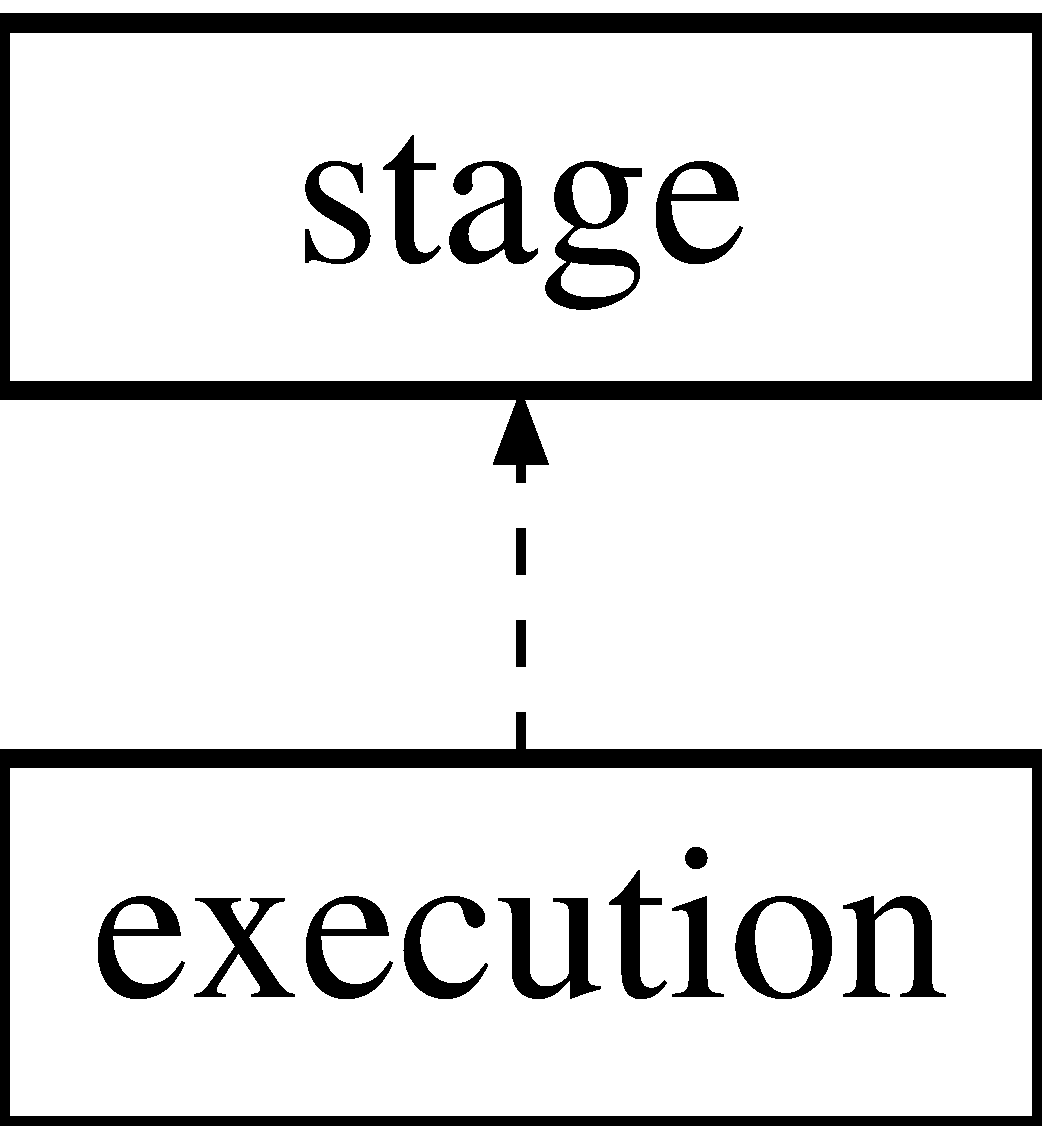
\includegraphics[height=2.000000cm]{classexecution}
\end{center}
\end{figure}
\subsection*{Public Member Functions}
\begin{DoxyCompactItemize}
\item 
\hyperlink{classexecution_a87b2844b03233ad768fa1ad67e1f93df}{execution} (\hyperlink{classport}{port}$<$ \hyperlink{classdynInstruction}{dynInstruction} $\ast$ $>$ \&scheduler\_\-to\_\-execution\_\-port, \hyperlink{classport}{port}$<$ \hyperlink{classdynInstruction}{dynInstruction} $\ast$ $>$ \&execution\_\-to\_\-scheduler\_\-port, \hyperlink{classport}{port}$<$ \hyperlink{classdynInstruction}{dynInstruction} $\ast$ $>$ \&execution\_\-to\_\-memory\_\-port, \hyperlink{classCAMtable}{CAMtable}$<$ \hyperlink{classdynInstruction}{dynInstruction} $\ast$ $>$ $\ast$\hyperlink{backend_2parser_8cpp_ad73ae25f81e6e99482f3fbd5ba9664ce}{iROB}, \hyperlink{global_2global_8h_a6fa2e24b8a418fa215e183264cbea3aa}{WIDTH} execution\_\-width, string stage\_\-name)
\item 
\hyperlink{classexecution_a686c28582542ecb0a4d41f9a649a6357}{$\sim$execution} ()
\item 
void \hyperlink{classexecution_a972207b1dde6a4bb8731c3fc0908bac6}{doEXECUTION} (\hyperlink{classsysClock}{sysClock} \&)
\item 
void \hyperlink{classexecution_a3e12895813ee78b1a7d2d10894db1204}{squashCtrl} (\hyperlink{classsysClock}{sysClock} \&)
\item 
void \hyperlink{classexecution_a243c30ebc13c7e2e6c1eb46a8fcac55e}{squash} (\hyperlink{classsysClock}{sysClock} \&)
\item 
void \hyperlink{classexecution_af6a859d27808b6db44c92b0ff79ef426}{regStat} (\hyperlink{classsysClock}{sysClock} \&clk)
\item 
\hyperlink{unit_2stage_8h_ab00e4188e8b8974fecb1dfd12764cbb1}{PIPE\_\-ACTIVITY} \hyperlink{classexecution_adc2d24703f3425df6107514535fea88b}{executionImpl} (\hyperlink{classsysClock}{sysClock} \&)
\item 
\hyperlink{unit_2stage_8h_a7de04de95175471455cf906d80af3968}{COMPLETE\_\-STATUS} \hyperlink{classexecution_a0c823fb6010268a0da3a706a9452d5e0}{completeIns} (\hyperlink{classsysClock}{sysClock} \&)
\item 
void \hyperlink{classexecution_a9271c55da8555444f0882c9027ab68a0}{forward} (\hyperlink{classdynInstruction}{dynInstruction} $\ast$, \hyperlink{global_2global_8h_a7e19a550ec11d1ed921deb20c22efb5b}{CYCLE}, \hyperlink{classsysClock}{sysClock} \&)
\end{DoxyCompactItemize}


\subsection{Constructor \& Destructor Documentation}
\hypertarget{classexecution_a87b2844b03233ad768fa1ad67e1f93df}{
\index{execution@{execution}!execution@{execution}}
\index{execution@{execution}!execution@{execution}}
\subsubsection[{execution}]{\setlength{\rightskip}{0pt plus 5cm}execution::execution (
\begin{DoxyParamCaption}
\item[{{\bf port}$<$ {\bf dynInstruction} $\ast$ $>$ \&}]{scheduler\_\-to\_\-execution\_\-port, }
\item[{{\bf port}$<$ {\bf dynInstruction} $\ast$ $>$ \&}]{execution\_\-to\_\-scheduler\_\-port, }
\item[{{\bf port}$<$ {\bf dynInstruction} $\ast$ $>$ \&}]{execution\_\-to\_\-memory\_\-port, }
\item[{{\bf CAMtable}$<$ {\bf dynInstruction} $\ast$ $>$ $\ast$}]{iROB, }
\item[{{\bf WIDTH}}]{execution\_\-width, }
\item[{string}]{stage\_\-name}
\end{DoxyParamCaption}
)}}
\label{classexecution_a87b2844b03233ad768fa1ad67e1f93df}

\begin{DoxyCode}
        : stage (execution_width, stage_name)
{
    _scheduler_to_execution_port = &scheduler_to_execution_port;
    _execution_to_scheduler_port = &execution_to_scheduler_port;
    _execution_to_memory_port = &execution_to_memory_port;
    _iROB = iROB;
    _aluExeUnits = new List<exeUnit*>;
    for (WIDTH i = 0; i < _stage_width; i++) {
        exeUnit* newEU = new exeUnit (1,  _eu_lat._alu_lat, ALU_EU); //TODO make 
      this config better with more EU types
        _aluExeUnits->Append (newEU);
    }
}
\end{DoxyCode}
\hypertarget{classexecution_a686c28582542ecb0a4d41f9a649a6357}{
\index{execution@{execution}!$\sim$execution@{$\sim$execution}}
\index{$\sim$execution@{$\sim$execution}!execution@{execution}}
\subsubsection[{$\sim$execution}]{\setlength{\rightskip}{0pt plus 5cm}execution::$\sim$execution (
\begin{DoxyParamCaption}
{}
\end{DoxyParamCaption}
)}}
\label{classexecution_a686c28582542ecb0a4d41f9a649a6357}

\begin{DoxyCode}
{}
\end{DoxyCode}


\subsection{Member Function Documentation}
\hypertarget{classexecution_a0c823fb6010268a0da3a706a9452d5e0}{
\index{execution@{execution}!completeIns@{completeIns}}
\index{completeIns@{completeIns}!execution@{execution}}
\subsubsection[{completeIns}]{\setlength{\rightskip}{0pt plus 5cm}{\bf COMPLETE\_\-STATUS} execution::completeIns (
\begin{DoxyParamCaption}
\item[{{\bf sysClock} \&}]{clk}
\end{DoxyParamCaption}
)}}
\label{classexecution_a0c823fb6010268a0da3a706a9452d5e0}

\begin{DoxyCode}
                                                     {
    g_var.setOldSquashSN ();
    for (WIDTH i = 0; i < _stage_width; i++) {
        exeUnit* EU = _aluExeUnits->Nth (i);
        dynInstruction* ins = EU->getEUins ();

        /* CHECKS */
        if (g_var.g_pipe_state == PIPE_FLUSH) break;
        if (ins != NULL && ins->getInsType () == MEM && 
            _execution_to_memory_port->getBuffState (clk.now ()) == FULL_BUFF) br
      eak;
        if (EU->getEUstate (clk.now (), true) != COMPLETE_EU) continue;

        /* COMPLETE INS */
        if (ins->getInsType () == MEM) {
            _execution_to_memory_port->pushBack (ins, clk.now ());
            ins->setPipeStage (MEM_ACCESS);
        } else {
            if (!g_RF_MGR.hasFreeWrPort (clk.now ())) break;
            ins->setPipeStage (COMPLETE);
            g_RF_MGR.writeToRF (ins);
        }
        EU->resetEU ();

        /* SQUASH DETECT */
        if (ins->isOnWrongPath ()) {
            g_var.setSquashSN (ins->getInsID ());
        }
        dbg.print (DBG_EXECUTION, "%s: %s %llu (cyc: %d)\n", _stage_name.c_str ()
      , "Complete ins", ins->getInsID (), clk.now ());
    }

    if (g_var.isOnWrongPath()) {
        dbg.print (DBG_EXECUTION, "%s: %s %llu %s (cyc: %d)\n", _stage_name.c_str
       (), "Ins on Wrong Path (ins: ", g_var.getSquashSN (), ")", clk.now ());
        return COMPLETE_SQUASH;
    }
    dbg.print (DBG_EXECUTION, "%s: %s (cyc: %d)\n", _stage_name.c_str (), "Ins on
       Right Path", clk.now ());
    return COMPLETE_NORMAL;
}
\end{DoxyCode}
\hypertarget{classexecution_a972207b1dde6a4bb8731c3fc0908bac6}{
\index{execution@{execution}!doEXECUTION@{doEXECUTION}}
\index{doEXECUTION@{doEXECUTION}!execution@{execution}}
\subsubsection[{doEXECUTION}]{\setlength{\rightskip}{0pt plus 5cm}void execution::doEXECUTION (
\begin{DoxyParamCaption}
\item[{{\bf sysClock} \&}]{clk}
\end{DoxyParamCaption}
)}}
\label{classexecution_a972207b1dde6a4bb8731c3fc0908bac6}

\begin{DoxyCode}
                                          {
    dbg.print (DBG_EXECUTION, "%s: (cyc: %d)\n", _stage_name.c_str (), clk.now ()
      );
    /* STAT */
    regStat (clk);
    PIPE_ACTIVITY pipe_stall = PIPE_STALL;

    /* WRITEBACK RESULT */
    COMPLETE_STATUS cmpl_status;
    cmpl_status = completeIns (clk);

    /* EXECUTE INS */
    if (cmpl_status == COMPLETE_NORMAL) {
        pipe_stall = executionImpl (clk);
    }

    /* SQUASH CONTROL */
    squashCtrl (clk);
    dbg.print (DBG_EXECUTION, "%s: %s %llu (cyc: %d)\n", _stage_name.c_str (), "P
      IPELINE STATE:", g_var.g_pipe_state, clk.now ());

    /* STAT */
    if (g_var.g_pipe_state != PIPE_NORMAL) s_squash_cycles++;
    if (pipe_stall == PIPE_STALL) s_stall_cycles++;
}
\end{DoxyCode}
\hypertarget{classexecution_adc2d24703f3425df6107514535fea88b}{
\index{execution@{execution}!executionImpl@{executionImpl}}
\index{executionImpl@{executionImpl}!execution@{execution}}
\subsubsection[{executionImpl}]{\setlength{\rightskip}{0pt plus 5cm}{\bf PIPE\_\-ACTIVITY} execution::executionImpl (
\begin{DoxyParamCaption}
\item[{{\bf sysClock} \&}]{clk}
\end{DoxyParamCaption}
)}}
\label{classexecution_adc2d24703f3425df6107514535fea88b}

\begin{DoxyCode}
                                                     {
    PIPE_ACTIVITY pipe_stall = PIPE_STALL;

    for (WIDTH i = 0; i < _stage_width; i++) {
        /* CHECKS */
        if (g_var.g_pipe_state == PIPE_WAIT_FLUSH || g_var.g_pipe_state == 
      PIPE_FLUSH) break;
        if (_scheduler_to_execution_port->getBuffState (clk.now ()) == 
      EMPTY_BUFF) break;
        if (!_scheduler_to_execution_port->isReady (clk.now ())) break;
        dynInstruction* ins = _scheduler_to_execution_port->getFront ();
        if (!g_RF_MGR.isReady (ins) || !g_RF_MGR.canReserveRF (ins)) break; // IN
      O EXE
        exeUnit* EU = _aluExeUnits->Nth (i);
        if (EU->getEUstate (clk.now (), false) != AVAILABLE_EU) continue;

        /* EXE INS */
        ins = _scheduler_to_execution_port->popFront (clk.now ());
        g_RF_MGR.reserveRF (ins);
        EU->_eu_timer.setNewTime (clk.now ());
        EU->setEUins (ins);
        EU->runEU ();
        ins->setPipeStage (EXECUTE);
        forward (ins, EU->_eu_timer.getLatency (), clk);
        dbg.print (DBG_EXECUTION, "%s: %s %llu (cyc: %d)\n", _stage_name.c_str ()
      , "Execute ins", ins->getInsID (), clk.now ());

        /* STAT */
        s_ins_cnt++;
        pipe_stall = PIPE_BUSY;
    }
    return pipe_stall;
}
\end{DoxyCode}
\hypertarget{classexecution_a9271c55da8555444f0882c9027ab68a0}{
\index{execution@{execution}!forward@{forward}}
\index{forward@{forward}!execution@{execution}}
\subsubsection[{forward}]{\setlength{\rightskip}{0pt plus 5cm}void execution::forward (
\begin{DoxyParamCaption}
\item[{{\bf dynInstruction} $\ast$}]{ins, }
\item[{{\bf CYCLE}}]{eu\_\-latency, }
\item[{{\bf sysClock} \&}]{clk}
\end{DoxyParamCaption}
)}}
\label{classexecution_a9271c55da8555444f0882c9027ab68a0}

\begin{DoxyCode}
                                                                             {
    if (_execution_to_scheduler_port->getBuffState (clk.now ()) == FULL_BUFF) ret
      urn;
    if (ins->getInsType () != MEM) {
        CYCLE cdb_ready_latency = eu_latency - 1;
        Assert (cdb_ready_latency >= 0);
        _execution_to_scheduler_port->pushBack (ins, clk.now (), cdb_ready_latenc
      y);
        dbg.print (DBG_EXECUTION, "%s: %s %llu (cyc: %d)\n", _stage_name.c_str ()
      , "Forward wr ops of ins", ins->getInsID (), clk.now ());
    }
}
\end{DoxyCode}
\hypertarget{classexecution_af6a859d27808b6db44c92b0ff79ef426}{
\index{execution@{execution}!regStat@{regStat}}
\index{regStat@{regStat}!execution@{execution}}
\subsubsection[{regStat}]{\setlength{\rightskip}{0pt plus 5cm}void execution::regStat (
\begin{DoxyParamCaption}
\item[{{\bf sysClock} \&}]{clk}
\end{DoxyParamCaption}
)}}
\label{classexecution_af6a859d27808b6db44c92b0ff79ef426}

\begin{DoxyCode}
                                      {
    _scheduler_to_execution_port->regStat (clk.now ());
}
\end{DoxyCode}
\hypertarget{classexecution_a243c30ebc13c7e2e6c1eb46a8fcac55e}{
\index{execution@{execution}!squash@{squash}}
\index{squash@{squash}!execution@{execution}}
\subsubsection[{squash}]{\setlength{\rightskip}{0pt plus 5cm}void execution::squash (
\begin{DoxyParamCaption}
\item[{{\bf sysClock} \&}]{clk}
\end{DoxyParamCaption}
)}}
\label{classexecution_a243c30ebc13c7e2e6c1eb46a8fcac55e}

\begin{DoxyCode}
                                     {
    dbg.print (DBG_SQUASH, "%s: %s (cyc: %d)\n", _stage_name.c_str (), "Execution
       Ports Flush", clk.now ());
    Assert (g_var.g_pipe_state == PIPE_FLUSH);
    INS_ID squashSeqNum = g_var.getSquashSN ();
    _execution_to_scheduler_port->flushPort (squashSeqNum, clk.now ());
    _execution_to_memory_port->flushPort (squashSeqNum, clk.now ());
}
\end{DoxyCode}
\hypertarget{classexecution_a3e12895813ee78b1a7d2d10894db1204}{
\index{execution@{execution}!squashCtrl@{squashCtrl}}
\index{squashCtrl@{squashCtrl}!execution@{execution}}
\subsubsection[{squashCtrl}]{\setlength{\rightskip}{0pt plus 5cm}void execution::squashCtrl (
\begin{DoxyParamCaption}
\item[{{\bf sysClock} \&}]{clk}
\end{DoxyParamCaption}
)}}
\label{classexecution_a3e12895813ee78b1a7d2d10894db1204}

\begin{DoxyCode}
                                         {
    string state_switch;
    if ((g_var.g_pipe_state == PIPE_NORMAL || g_var.g_pipe_state == 
      PIPE_SQUASH_ROB) && 
        g_var.g_squash_seq_num != g_var.g_old_squash_seq_num) {
        g_var.g_pipe_state = PIPE_WAIT_FLUSH;
        state_switch =  "PIPE_NORMAL -> PIPE_WAIT_FLUSH";
    } else if (g_var.g_pipe_state == PIPE_NORMAL) {
        g_var.resetSquashSN ();
        return;
    } else if (g_var.g_pipe_state == PIPE_WAIT_FLUSH) {
        for (WIDTH i = 0; i < _stage_width; i++) {
            exeUnit* EU = _aluExeUnits->Nth (i);
            if (EU->getEUstate (clk.now (), false) != AVAILABLE_EU) return;
        }
        g_var.g_pipe_state = PIPE_FLUSH;
        state_switch =  "PIPE_WAIT_FLUSH -> PIPE_FLUSH";
        for (WIDTH i = 0; i < _stage_width; i++) {
            exeUnit* EU = _aluExeUnits->Nth (i);
            EU->resetEU ();
        }
        squash (clk);
    } else if (g_var.g_pipe_state == PIPE_FLUSH) {
        g_var.g_pipe_state = PIPE_DRAIN;
        state_switch =  "PIPE_FLUSH -> PIPE_DRAIN";
    } else if (g_var.g_pipe_state == PIPE_DRAIN && _iROB->hasFreeRdPort (clk.now 
      ()) && 
               _iROB->getFront()->getInsID () >= g_var.g_squash_seq_num) {
        g_var.g_pipe_state = PIPE_SQUASH_ROB;
        state_switch =  "PIPE_DRAIN -> PIPE_SQUASH_ROB";
    } else if (g_var.g_pipe_state == PIPE_SQUASH_ROB && _iROB->getTableSize() == 
      0) {
        g_var.resetSquashSN ();
        g_var.g_pipe_state = PIPE_NORMAL;
        state_switch =  "PIPE_SQUASH_ROB -> PIPE_NORMAL";
        g_RF_MGR.resetRF ();
    } else {
        return; /* No state change */
    }
    dbg.print (DBG_EXECUTION, "%s: %s (cyc: %d)\n", _stage_name.c_str (), state_s
      witch.c_str(), clk.now ());
}
\end{DoxyCode}


The documentation for this class was generated from the following files:\begin{DoxyCompactItemize}
\item 
/home/milad/esc\_\-project/svn/PARS/src/backend/ino/\hyperlink{ino_2execution_8h}{execution.h}\item 
/home/milad/esc\_\-project/svn/PARS/src/backend/ino/\hyperlink{ino_2execution_8cpp}{execution.cpp}\end{DoxyCompactItemize}

\hypertarget{structexeUnit}{
\section{exeUnit Struct Reference}
\label{structexeUnit}\index{exeUnit@{exeUnit}}
}


{\ttfamily \#include $<$exeUnit.h$>$}

\subsection*{Public Member Functions}
\begin{DoxyCompactItemize}
\item 
\hyperlink{structexeUnit_af9048405bad98db15cdefb05bf7b842c}{exeUnit} (\hyperlink{global_2global_8h_a7e19a550ec11d1ed921deb20c22efb5b}{CYCLE} \hyperlink{bkEnd_8cpp_ada310e7f72b38fadd4b24d80ed3438ee}{start}, \hyperlink{global_2global_8h_a7e19a550ec11d1ed921deb20c22efb5b}{CYCLE} latency, \hyperlink{exeUnit_8h_a8184e36081fa22a84c7488c1eaeb0f5d}{EU\_\-TYPE} eu\_\-type)
\item 
\hyperlink{exeUnit_8h_ac578f59a761f9106ba1a8414e02ab6d8}{EU\_\-STATE} \hyperlink{structexeUnit_a739cfd78a98068a64fb2e807f49c4312}{getEUstate} (\hyperlink{global_2global_8h_a7e19a550ec11d1ed921deb20c22efb5b}{CYCLE} now, bool limit\_\-eu\_\-state\_\-access)
\item 
void \hyperlink{structexeUnit_a69498b2ca8353a14447a5596e768fc55}{runEU} ()
\item 
void \hyperlink{structexeUnit_ad9a4840a6956e01419327ba3123683dd}{setEUins} (\hyperlink{classdynInstruction}{dynInstruction} $\ast$ins)
\item 
\hyperlink{classdynInstruction}{dynInstruction} $\ast$ \hyperlink{structexeUnit_a5414837e2e071fc0180c0326cc33370f}{getEUins} ()
\item 
void \hyperlink{structexeUnit_a31fd51a344347d96c9be688de8e0f97a}{resetEU} ()
\end{DoxyCompactItemize}
\subsection*{Public Attributes}
\begin{DoxyCompactItemize}
\item 
\hyperlink{structtimer}{timer} \hyperlink{structexeUnit_a5dc187ea49bad94bbea24f18232500dd}{\_\-eu\_\-timer}
\end{DoxyCompactItemize}


\subsection{Constructor \& Destructor Documentation}
\hypertarget{structexeUnit_af9048405bad98db15cdefb05bf7b842c}{
\index{exeUnit@{exeUnit}!exeUnit@{exeUnit}}
\index{exeUnit@{exeUnit}!exeUnit@{exeUnit}}
\subsubsection[{exeUnit}]{\setlength{\rightskip}{0pt plus 5cm}exeUnit::exeUnit (
\begin{DoxyParamCaption}
\item[{{\bf CYCLE}}]{start, }
\item[{{\bf CYCLE}}]{latency, }
\item[{{\bf EU\_\-TYPE}}]{eu\_\-type}
\end{DoxyParamCaption}
)\hspace{0.3cm}{\ttfamily  \mbox{[}inline\mbox{]}}}}
\label{structexeUnit_af9048405bad98db15cdefb05bf7b842c}

\begin{DoxyCode}
        : _eu_timer (start, latency),
          _eu_type (eu_type)
    {
        _eu_ins = NULL;
        _eu_state = AVAILABLE_EU;
    }
\end{DoxyCode}


\subsection{Member Function Documentation}
\hypertarget{structexeUnit_a5414837e2e071fc0180c0326cc33370f}{
\index{exeUnit@{exeUnit}!getEUins@{getEUins}}
\index{getEUins@{getEUins}!exeUnit@{exeUnit}}
\subsubsection[{getEUins}]{\setlength{\rightskip}{0pt plus 5cm}{\bf dynInstruction}$\ast$ exeUnit::getEUins (
\begin{DoxyParamCaption}
{}
\end{DoxyParamCaption}
)\hspace{0.3cm}{\ttfamily  \mbox{[}inline\mbox{]}}}}
\label{structexeUnit_a5414837e2e071fc0180c0326cc33370f}

\begin{DoxyCode}
{return _eu_ins;}
\end{DoxyCode}
\hypertarget{structexeUnit_a739cfd78a98068a64fb2e807f49c4312}{
\index{exeUnit@{exeUnit}!getEUstate@{getEUstate}}
\index{getEUstate@{getEUstate}!exeUnit@{exeUnit}}
\subsubsection[{getEUstate}]{\setlength{\rightskip}{0pt plus 5cm}{\bf EU\_\-STATE} exeUnit::getEUstate (
\begin{DoxyParamCaption}
\item[{{\bf CYCLE}}]{now, }
\item[{bool}]{limit\_\-eu\_\-state\_\-access}
\end{DoxyParamCaption}
)\hspace{0.3cm}{\ttfamily  \mbox{[}inline\mbox{]}}}}
\label{structexeUnit_a739cfd78a98068a64fb2e807f49c4312}

\begin{DoxyCode}
                                                                {
        if (!limit_eu_state_access) {
            return _eu_state;
        } else {
            if (_eu_state == RUNNING_EU && now >= _eu_timer.getStopTime ()) {
                _eu_state = COMPLETE_EU;
            } else if (_eu_state == RUNNING_EU) {
                _eu_state = RUNNING_EU;
            } else if (_eu_state == COMPLETE_EU) {
                _eu_state = AVAILABLE_EU;
            } else if (_eu_state == AVAILABLE_EU) {
                _eu_state = AVAILABLE_EU;
            } else {
                Assert (true == false && "invalid EU state");
            }
            return _eu_state;
        }
    }
\end{DoxyCode}
\hypertarget{structexeUnit_a31fd51a344347d96c9be688de8e0f97a}{
\index{exeUnit@{exeUnit}!resetEU@{resetEU}}
\index{resetEU@{resetEU}!exeUnit@{exeUnit}}
\subsubsection[{resetEU}]{\setlength{\rightskip}{0pt plus 5cm}void exeUnit::resetEU (
\begin{DoxyParamCaption}
{}
\end{DoxyParamCaption}
)\hspace{0.3cm}{\ttfamily  \mbox{[}inline\mbox{]}}}}
\label{structexeUnit_a31fd51a344347d96c9be688de8e0f97a}

\begin{DoxyCode}
{_eu_ins = NULL; _eu_state = AVAILABLE_EU;}
\end{DoxyCode}
\hypertarget{structexeUnit_a69498b2ca8353a14447a5596e768fc55}{
\index{exeUnit@{exeUnit}!runEU@{runEU}}
\index{runEU@{runEU}!exeUnit@{exeUnit}}
\subsubsection[{runEU}]{\setlength{\rightskip}{0pt plus 5cm}void exeUnit::runEU (
\begin{DoxyParamCaption}
{}
\end{DoxyParamCaption}
)\hspace{0.3cm}{\ttfamily  \mbox{[}inline\mbox{]}}}}
\label{structexeUnit_a69498b2ca8353a14447a5596e768fc55}

\begin{DoxyCode}
                  {
        Assert (_eu_state == AVAILABLE_EU);
        _eu_state = RUNNING_EU;
    }
\end{DoxyCode}
\hypertarget{structexeUnit_ad9a4840a6956e01419327ba3123683dd}{
\index{exeUnit@{exeUnit}!setEUins@{setEUins}}
\index{setEUins@{setEUins}!exeUnit@{exeUnit}}
\subsubsection[{setEUins}]{\setlength{\rightskip}{0pt plus 5cm}void exeUnit::setEUins (
\begin{DoxyParamCaption}
\item[{{\bf dynInstruction} $\ast$}]{ins}
\end{DoxyParamCaption}
)\hspace{0.3cm}{\ttfamily  \mbox{[}inline\mbox{]}}}}
\label{structexeUnit_ad9a4840a6956e01419327ba3123683dd}

\begin{DoxyCode}
{ Assert (_eu_ins == NULL); _eu_ins = ins;}
\end{DoxyCode}


\subsection{Member Data Documentation}
\hypertarget{structexeUnit_a5dc187ea49bad94bbea24f18232500dd}{
\index{exeUnit@{exeUnit}!\_\-eu\_\-timer@{\_\-eu\_\-timer}}
\index{\_\-eu\_\-timer@{\_\-eu\_\-timer}!exeUnit@{exeUnit}}
\subsubsection[{\_\-eu\_\-timer}]{\setlength{\rightskip}{0pt plus 5cm}{\bf timer} {\bf exeUnit::\_\-eu\_\-timer}}}
\label{structexeUnit_a5dc187ea49bad94bbea24f18232500dd}


The documentation for this struct was generated from the following file:\begin{DoxyCompactItemize}
\item 
/home/milad/esc\_\-project/svn/PARS/src/backend/unit/\hyperlink{exeUnit_8h}{exeUnit.h}\end{DoxyCompactItemize}

\hypertarget{structexeUnitLat}{
\section{exeUnitLat Struct Reference}
\label{structexeUnitLat}\index{exeUnitLat@{exeUnitLat}}
}


{\ttfamily \#include $<$exeUnit.h$>$}

\subsection*{Public Member Functions}
\begin{DoxyCompactItemize}
\item 
\hyperlink{structexeUnitLat_acd7bea2d80b4acddfd631aaca75fa8b5}{exeUnitLat} ()
\end{DoxyCompactItemize}
\subsection*{Public Attributes}
\begin{DoxyCompactItemize}
\item 
const \hyperlink{global_2global_8h_a7e19a550ec11d1ed921deb20c22efb5b}{CYCLE} \hyperlink{structexeUnitLat_a1c6fbd51db44097cab33015d4ee9dd81}{\_\-alu\_\-lat}
\item 
const \hyperlink{global_2global_8h_a7e19a550ec11d1ed921deb20c22efb5b}{CYCLE} \hyperlink{structexeUnitLat_a3eaf6d977e10668f9f9641601c2e155d}{\_\-fpu\_\-lat}
\item 
const \hyperlink{global_2global_8h_a7e19a550ec11d1ed921deb20c22efb5b}{CYCLE} \hyperlink{structexeUnitLat_a56f987ed90a23321279e330e068262f8}{\_\-bru\_\-lat}
\item 
const \hyperlink{global_2global_8h_a7e19a550ec11d1ed921deb20c22efb5b}{CYCLE} \hyperlink{structexeUnitLat_a2e0a0b29c7d4cd40492fe25740302c72}{\_\-st\_\-buff\_\-lat}
\item 
const \hyperlink{global_2global_8h_a7e19a550ec11d1ed921deb20c22efb5b}{CYCLE} \hyperlink{structexeUnitLat_a3c5ce17975afa47ae136e8355e328c3b}{\_\-l1\_\-lat}
\item 
const \hyperlink{global_2global_8h_a7e19a550ec11d1ed921deb20c22efb5b}{CYCLE} \hyperlink{structexeUnitLat_a0a5e96d306ef23a2d69c8e97d62b27fd}{\_\-l2\_\-lat}
\item 
const \hyperlink{global_2global_8h_a7e19a550ec11d1ed921deb20c22efb5b}{CYCLE} \hyperlink{structexeUnitLat_ae34f390b9e9b8e9d792a6656b801eca4}{\_\-l3\_\-lat}
\item 
const \hyperlink{global_2global_8h_a7e19a550ec11d1ed921deb20c22efb5b}{CYCLE} \hyperlink{structexeUnitLat_a0478d29cba99e1c3849dceb6ecfca973}{\_\-mem\_\-lat}
\end{DoxyCompactItemize}


\subsection{Constructor \& Destructor Documentation}
\hypertarget{structexeUnitLat_acd7bea2d80b4acddfd631aaca75fa8b5}{
\index{exeUnitLat@{exeUnitLat}!exeUnitLat@{exeUnitLat}}
\index{exeUnitLat@{exeUnitLat}!exeUnitLat@{exeUnitLat}}
\subsubsection[{exeUnitLat}]{\setlength{\rightskip}{0pt plus 5cm}exeUnitLat::exeUnitLat (
\begin{DoxyParamCaption}
{}
\end{DoxyParamCaption}
)\hspace{0.3cm}{\ttfamily  \mbox{[}inline\mbox{]}}}}
\label{structexeUnitLat_acd7bea2d80b4acddfd631aaca75fa8b5}

\begin{DoxyCode}
        : _alu_lat (1),
          _fpu_lat (5),
          _bru_lat (1),
          _st_buff_lat (1),
          _l1_lat (1),
          _l2_lat (1),
          _l3_lat (1),
          _mem_lat (1)
    { }
\end{DoxyCode}


\subsection{Member Data Documentation}
\hypertarget{structexeUnitLat_a1c6fbd51db44097cab33015d4ee9dd81}{
\index{exeUnitLat@{exeUnitLat}!\_\-alu\_\-lat@{\_\-alu\_\-lat}}
\index{\_\-alu\_\-lat@{\_\-alu\_\-lat}!exeUnitLat@{exeUnitLat}}
\subsubsection[{\_\-alu\_\-lat}]{\setlength{\rightskip}{0pt plus 5cm}const {\bf CYCLE} {\bf exeUnitLat::\_\-alu\_\-lat}}}
\label{structexeUnitLat_a1c6fbd51db44097cab33015d4ee9dd81}
\hypertarget{structexeUnitLat_a56f987ed90a23321279e330e068262f8}{
\index{exeUnitLat@{exeUnitLat}!\_\-bru\_\-lat@{\_\-bru\_\-lat}}
\index{\_\-bru\_\-lat@{\_\-bru\_\-lat}!exeUnitLat@{exeUnitLat}}
\subsubsection[{\_\-bru\_\-lat}]{\setlength{\rightskip}{0pt plus 5cm}const {\bf CYCLE} {\bf exeUnitLat::\_\-bru\_\-lat}}}
\label{structexeUnitLat_a56f987ed90a23321279e330e068262f8}
\hypertarget{structexeUnitLat_a3eaf6d977e10668f9f9641601c2e155d}{
\index{exeUnitLat@{exeUnitLat}!\_\-fpu\_\-lat@{\_\-fpu\_\-lat}}
\index{\_\-fpu\_\-lat@{\_\-fpu\_\-lat}!exeUnitLat@{exeUnitLat}}
\subsubsection[{\_\-fpu\_\-lat}]{\setlength{\rightskip}{0pt plus 5cm}const {\bf CYCLE} {\bf exeUnitLat::\_\-fpu\_\-lat}}}
\label{structexeUnitLat_a3eaf6d977e10668f9f9641601c2e155d}
\hypertarget{structexeUnitLat_a3c5ce17975afa47ae136e8355e328c3b}{
\index{exeUnitLat@{exeUnitLat}!\_\-l1\_\-lat@{\_\-l1\_\-lat}}
\index{\_\-l1\_\-lat@{\_\-l1\_\-lat}!exeUnitLat@{exeUnitLat}}
\subsubsection[{\_\-l1\_\-lat}]{\setlength{\rightskip}{0pt plus 5cm}const {\bf CYCLE} {\bf exeUnitLat::\_\-l1\_\-lat}}}
\label{structexeUnitLat_a3c5ce17975afa47ae136e8355e328c3b}
\hypertarget{structexeUnitLat_a0a5e96d306ef23a2d69c8e97d62b27fd}{
\index{exeUnitLat@{exeUnitLat}!\_\-l2\_\-lat@{\_\-l2\_\-lat}}
\index{\_\-l2\_\-lat@{\_\-l2\_\-lat}!exeUnitLat@{exeUnitLat}}
\subsubsection[{\_\-l2\_\-lat}]{\setlength{\rightskip}{0pt plus 5cm}const {\bf CYCLE} {\bf exeUnitLat::\_\-l2\_\-lat}}}
\label{structexeUnitLat_a0a5e96d306ef23a2d69c8e97d62b27fd}
\hypertarget{structexeUnitLat_ae34f390b9e9b8e9d792a6656b801eca4}{
\index{exeUnitLat@{exeUnitLat}!\_\-l3\_\-lat@{\_\-l3\_\-lat}}
\index{\_\-l3\_\-lat@{\_\-l3\_\-lat}!exeUnitLat@{exeUnitLat}}
\subsubsection[{\_\-l3\_\-lat}]{\setlength{\rightskip}{0pt plus 5cm}const {\bf CYCLE} {\bf exeUnitLat::\_\-l3\_\-lat}}}
\label{structexeUnitLat_ae34f390b9e9b8e9d792a6656b801eca4}
\hypertarget{structexeUnitLat_a0478d29cba99e1c3849dceb6ecfca973}{
\index{exeUnitLat@{exeUnitLat}!\_\-mem\_\-lat@{\_\-mem\_\-lat}}
\index{\_\-mem\_\-lat@{\_\-mem\_\-lat}!exeUnitLat@{exeUnitLat}}
\subsubsection[{\_\-mem\_\-lat}]{\setlength{\rightskip}{0pt plus 5cm}const {\bf CYCLE} {\bf exeUnitLat::\_\-mem\_\-lat}}}
\label{structexeUnitLat_a0478d29cba99e1c3849dceb6ecfca973}
\hypertarget{structexeUnitLat_a2e0a0b29c7d4cd40492fe25740302c72}{
\index{exeUnitLat@{exeUnitLat}!\_\-st\_\-buff\_\-lat@{\_\-st\_\-buff\_\-lat}}
\index{\_\-st\_\-buff\_\-lat@{\_\-st\_\-buff\_\-lat}!exeUnitLat@{exeUnitLat}}
\subsubsection[{\_\-st\_\-buff\_\-lat}]{\setlength{\rightskip}{0pt plus 5cm}const {\bf CYCLE} {\bf exeUnitLat::\_\-st\_\-buff\_\-lat}}}
\label{structexeUnitLat_a2e0a0b29c7d4cd40492fe25740302c72}


The documentation for this struct was generated from the following file:\begin{DoxyCompactItemize}
\item 
/home/milad/esc\_\-project/svn/PARS/src/backend/unit/\hyperlink{exeUnit_8h}{exeUnit.h}\end{DoxyCompactItemize}

\input{structExplain}
\input{structExpr}
\input{structExprList}
\input{structExprList_1_1ExprList__item}
\input{structExprSpan}
\input{classMemory_1_1Factory}
\hypertarget{classfetch}{
\section{fetch Class Reference}
\label{classfetch}\index{fetch@{fetch}}
}


{\ttfamily \#include $<$fetch.h$>$}



Inheritance diagram for fetch:


Collaboration diagram for fetch:
\subsection*{Public Member Functions}
\begin{DoxyCompactItemize}
\item 
\hyperlink{classfetch_ac35d86b42890d4facb56666a58548a8d}{fetch} ()
\item 
\hyperlink{classfetch_a7bb4278b048d48d4225cb44b6553b3d6}{$\sim$fetch} ()
\item 
\hyperlink{classfetch_ad7f7cc7347c967a7843194684f3c3b21}{fetch} (\hyperlink{classport}{port}$<$ \hyperlink{classdynInstruction}{dynInstruction} $\ast$ $>$ \&bp\_\-to\_\-fetch\_\-port, \hyperlink{classport}{port}$<$ \hyperlink{classdynInstruction}{dynInstruction} $\ast$ $>$ \&fetch\_\-to\_\-decode\_\-port, \hyperlink{classport}{port}$<$ \hyperlink{classdynInstruction}{dynInstruction} $\ast$ $>$ \&fetch\_\-to\_\-bp\_\-port, \hyperlink{global_2global_8h_a6fa2e24b8a418fa215e183264cbea3aa}{WIDTH} fetch\_\-width, string stage\_\-name)
\item 
\hyperlink{classfetch_a7bb4278b048d48d4225cb44b6553b3d6}{$\sim$fetch} ()
\item 
\hyperlink{unit_2stage_8h_ac68af0001af4b7049b2435ded74c4e5e}{SIM\_\-MODE} \hyperlink{classfetch_abe2124748be0ac8b2e2b516203f9b194}{doFETCH} (\hyperlink{classsysClock}{sysClock} \&clk)
\item 
\hyperlink{unit_2stage_8h_ab00e4188e8b8974fecb1dfd12764cbb1}{PIPE\_\-ACTIVITY} \hyperlink{classfetch_af1aaa5a5c78172ec27dae140c7dc3ab3}{fetchImpl} (\hyperlink{classsysClock}{sysClock} \&clk)
\item 
void \hyperlink{classfetch_a39b22ed50d3b51ebe311be86343fed2a}{squash} (\hyperlink{classsysClock}{sysClock} \&clk)
\item 
void \hyperlink{classfetch_afd8c8e8e16f0f288d1090d59a85c2281}{regStat} (\hyperlink{classsysClock}{sysClock} \&clk)
\end{DoxyCompactItemize}


\subsection{Constructor \& Destructor Documentation}
\hypertarget{classfetch_ac35d86b42890d4facb56666a58548a8d}{
\index{fetch@{fetch}!fetch@{fetch}}
\index{fetch@{fetch}!fetch@{fetch}}
\subsubsection[{fetch}]{\setlength{\rightskip}{0pt plus 5cm}fetch::fetch (
\begin{DoxyParamCaption}
{}
\end{DoxyParamCaption}
)}}
\label{classfetch_ac35d86b42890d4facb56666a58548a8d}

\begin{DoxyCode}
             {
        _insBuff = new List<instruction*>;
}
\end{DoxyCode}
\hypertarget{classfetch_a7bb4278b048d48d4225cb44b6553b3d6}{
\index{fetch@{fetch}!$\sim$fetch@{$\sim$fetch}}
\index{$\sim$fetch@{$\sim$fetch}!fetch@{fetch}}
\subsubsection[{$\sim$fetch}]{\setlength{\rightskip}{0pt plus 5cm}fetch::$\sim$fetch (
\begin{DoxyParamCaption}
{}
\end{DoxyParamCaption}
)}}
\label{classfetch_a7bb4278b048d48d4225cb44b6553b3d6}

\begin{DoxyCode}
              {
        delete _insBuff;
}
\end{DoxyCode}
\hypertarget{classfetch_ad7f7cc7347c967a7843194684f3c3b21}{
\index{fetch@{fetch}!fetch@{fetch}}
\index{fetch@{fetch}!fetch@{fetch}}
\subsubsection[{fetch}]{\setlength{\rightskip}{0pt plus 5cm}fetch::fetch (
\begin{DoxyParamCaption}
\item[{{\bf port}$<$ {\bf dynInstruction} $\ast$ $>$ \&}]{bp\_\-to\_\-fetch\_\-port, }
\item[{{\bf port}$<$ {\bf dynInstruction} $\ast$ $>$ \&}]{fetch\_\-to\_\-decode\_\-port, }
\item[{{\bf port}$<$ {\bf dynInstruction} $\ast$ $>$ \&}]{fetch\_\-to\_\-bp\_\-port, }
\item[{{\bf WIDTH}}]{fetch\_\-width, }
\item[{string}]{stage\_\-name}
\end{DoxyParamCaption}
)}}
\label{classfetch_ad7f7cc7347c967a7843194684f3c3b21}

\begin{DoxyCode}
        : stage(fetch_width, stage_name)
{
    _bp_to_fetch_port = &bp_to_fetch_port;
    _fetch_to_bp_port = &fetch_to_bp_port;
    _fetch_to_decode_port = &fetch_to_decode_port;
    _insListIndx = 0;
    _switch_to_frontend = false;
}
\end{DoxyCode}
\hypertarget{classfetch_a7bb4278b048d48d4225cb44b6553b3d6}{
\index{fetch@{fetch}!$\sim$fetch@{$\sim$fetch}}
\index{$\sim$fetch@{$\sim$fetch}!fetch@{fetch}}
\subsubsection[{$\sim$fetch}]{\setlength{\rightskip}{0pt plus 5cm}fetch::$\sim$fetch (
\begin{DoxyParamCaption}
{}
\end{DoxyParamCaption}
)}}
\label{classfetch_a7bb4278b048d48d4225cb44b6553b3d6}


\subsection{Member Function Documentation}
\hypertarget{classfetch_abe2124748be0ac8b2e2b516203f9b194}{
\index{fetch@{fetch}!doFETCH@{doFETCH}}
\index{doFETCH@{doFETCH}!fetch@{fetch}}
\subsubsection[{doFETCH}]{\setlength{\rightskip}{0pt plus 5cm}{\bf SIM\_\-MODE} fetch::doFETCH (
\begin{DoxyParamCaption}
\item[{{\bf sysClock} \&}]{clk}
\end{DoxyParamCaption}
)}}
\label{classfetch_abe2124748be0ac8b2e2b516203f9b194}

\begin{DoxyCode}
                                      {
    dbg.print (DBG_FETCH, "%s: (cyc: %d)\n", _stage_name.c_str (), clk.now ());
    /* STAT */
    regStat (clk);
    PIPE_ACTIVITY pipe_stall = PIPE_STALL;

    /* SQUASH HANDLING */
    if (g_var.g_pipe_state == PIPE_FLUSH) { squash (clk); }
    if (g_var.g_pipe_state == PIPE_NORMAL) {
        pipe_stall = fetchImpl (clk);
    }

    /* STAT */
    if (pipe_stall == PIPE_STALL) s_stall_cycles++;

    if (_switch_to_frontend) {
        _switch_to_frontend = false;
        return FRONT_END;
    }
        return BACK_END;
}
\end{DoxyCode}


Here is the call graph for this function:




Here is the caller graph for this function:


\hypertarget{classfetch_af1aaa5a5c78172ec27dae140c7dc3ab3}{
\index{fetch@{fetch}!fetchImpl@{fetchImpl}}
\index{fetchImpl@{fetchImpl}!fetch@{fetch}}
\subsubsection[{fetchImpl}]{\setlength{\rightskip}{0pt plus 5cm}{\bf PIPE\_\-ACTIVITY} fetch::fetchImpl (
\begin{DoxyParamCaption}
\item[{{\bf sysClock} \&}]{clk}
\end{DoxyParamCaption}
)}}
\label{classfetch_af1aaa5a5c78172ec27dae140c7dc3ab3}

\begin{DoxyCode}
                                             {
    PIPE_ACTIVITY pipe_stall = PIPE_STALL;
        for (WIDTH i = 0; i < _stage_width; i++) {
                /* CHECKS */
        if (g_var.isCodeCacheEmpty()) { _switch_to_frontend = true; break; }
                if (_fetch_to_decode_port->getBuffState (clk.now ()) == 
      FULL_BUFF) break;

        /* FETCH INS */
        dynInstruction* ins = g_var.popCodeCache();
        ins->setPipeStage(FETCH);
        g_var.remFromCodeCache ();
                _fetch_to_decode_port->pushBack(ins, clk.now());
        dbg.print (DBG_FETCH, "%s: %s %llu (cyc: %d)\n", _stage_name.c_str (), "F
      etch ins", ins->getInsID (), clk.now ());

        /* STAT */
        s_ins_cnt++;
        pipe_stall = PIPE_BUSY;
        }
    return pipe_stall;
}
\end{DoxyCode}


Here is the call graph for this function:




Here is the caller graph for this function:


\hypertarget{classfetch_afd8c8e8e16f0f288d1090d59a85c2281}{
\index{fetch@{fetch}!regStat@{regStat}}
\index{regStat@{regStat}!fetch@{fetch}}
\subsubsection[{regStat}]{\setlength{\rightskip}{0pt plus 5cm}void fetch::regStat (
\begin{DoxyParamCaption}
\item[{{\bf sysClock} \&}]{clk}
\end{DoxyParamCaption}
)}}
\label{classfetch_afd8c8e8e16f0f288d1090d59a85c2281}

\begin{DoxyCode}
                                  {
    _bp_to_fetch_port->regStat (clk.now ());
}
\end{DoxyCode}


Here is the call graph for this function:




Here is the caller graph for this function:


\hypertarget{classfetch_a39b22ed50d3b51ebe311be86343fed2a}{
\index{fetch@{fetch}!squash@{squash}}
\index{squash@{squash}!fetch@{fetch}}
\subsubsection[{squash}]{\setlength{\rightskip}{0pt plus 5cm}void fetch::squash (
\begin{DoxyParamCaption}
\item[{{\bf sysClock} \&}]{clk}
\end{DoxyParamCaption}
)}}
\label{classfetch_a39b22ed50d3b51ebe311be86343fed2a}

\begin{DoxyCode}
                                 {
    dbg.print (DBG_SQUASH, "%s: %s (cyc: %d)\n", _stage_name.c_str (), "Fetch Por
      t Flush", clk.now ());
    Assert (g_var.g_pipe_state == PIPE_FLUSH);
    INS_ID squashSeqNum = g_var.getSquashSN();
    _fetch_to_decode_port->flushPort (squashSeqNum, clk.now ());
    _fetch_to_bp_port->flushPort (squashSeqNum, clk.now ());
}
\end{DoxyCode}


Here is the call graph for this function:




Here is the caller graph for this function:




The documentation for this class was generated from the following files:\begin{DoxyCompactItemize}
\item 
/home/milad/esc\_\-project/svn/PARS/src/backend/\hyperlink{fetch_8h}{fetch.h}\item 
/home/milad/esc\_\-project/svn/PARS/src/backend/ino/\hyperlink{ino_2fetch_8h}{fetch.h}\item 
/home/milad/esc\_\-project/svn/PARS/src/backend/\hyperlink{fetch_8cpp}{fetch.cpp}\item 
/home/milad/esc\_\-project/svn/PARS/src/backend/ino/\hyperlink{ino_2fetch_8cpp}{fetch.cpp}\end{DoxyCompactItemize}

\hypertarget{classFIFOtable}{
\section{FIFOtable$<$ tableType\_\-T $>$ Class Template Reference}
\label{classFIFOtable}\index{FIFOtable@{FIFOtable}}
}


{\ttfamily \#include $<$table.h$>$}



Inheritance diagram for FIFOtable$<$ tableType\_\-T $>$:


Collaboration diagram for FIFOtable$<$ tableType\_\-T $>$:
\subsection*{Public Member Functions}
\begin{DoxyCompactItemize}
\item 
\hyperlink{classFIFOtable_ad5ff5e6a3e0bf0b409f8b6d6ab5e4a5c}{FIFOtable} (\hyperlink{global_2global_8h_ad7ec63c69447a2b630929c8e0197860d}{LENGTH}, \hyperlink{global_2global_8h_a6fa2e24b8a418fa215e183264cbea3aa}{WIDTH}, \hyperlink{global_2global_8h_a6fa2e24b8a418fa215e183264cbea3aa}{WIDTH}, string)
\item 
\hyperlink{classFIFOtable_aed7aeb790ce1f0fbb429d645597554b5}{$\sim$FIFOtable} ()
\item 
tableType\_\-T \hyperlink{classFIFOtable_a96f42bb7a9f9b845970893bfe95ed2fb}{getFront} ()
\item 
tableType\_\-T \hyperlink{classFIFOtable_ace3286538766dfa4499d149767ac153f}{popFront} ()
\end{DoxyCompactItemize}
\subsubsection*{template$<$typename tableType\_\-T$>$ class FIFOtable$<$ tableType\_\-T $>$}



\subsection{Constructor \& Destructor Documentation}
\hypertarget{classFIFOtable_ad5ff5e6a3e0bf0b409f8b6d6ab5e4a5c}{
\index{FIFOtable@{FIFOtable}!FIFOtable@{FIFOtable}}
\index{FIFOtable@{FIFOtable}!FIFOtable@{FIFOtable}}
\subsubsection[{FIFOtable}]{\setlength{\rightskip}{0pt plus 5cm}template$<$typename tableType\_\-T $>$ {\bf FIFOtable}$<$ tableType\_\-T $>$::{\bf FIFOtable} (
\begin{DoxyParamCaption}
\item[{{\bf LENGTH}}]{len = {\ttfamily 1}, }
\item[{{\bf WIDTH}}]{rd\_\-port\_\-cnt = {\ttfamily 1}, }
\item[{{\bf WIDTH}}]{wr\_\-port\_\-cnt = {\ttfamily 1}, }
\item[{string}]{table\_\-name = {\ttfamily \char`\"{}FIFOtable$<$~tableType\_\-T~$>$\char`\"{}}}
\end{DoxyParamCaption}
)}}
\label{classFIFOtable_ad5ff5e6a3e0bf0b409f8b6d6ab5e4a5c}

\begin{DoxyCode}
    : table<tableType_T> (len, FIFO_ARRAY,
                          wr_port_cnt, rd_port_cnt, table_name)
{}
\end{DoxyCode}
\hypertarget{classFIFOtable_aed7aeb790ce1f0fbb429d645597554b5}{
\index{FIFOtable@{FIFOtable}!$\sim$FIFOtable@{$\sim$FIFOtable}}
\index{$\sim$FIFOtable@{$\sim$FIFOtable}!FIFOtable@{FIFOtable}}
\subsubsection[{$\sim$FIFOtable}]{\setlength{\rightskip}{0pt plus 5cm}template$<$typename tableType\_\-T$>$ {\bf FIFOtable}$<$ tableType\_\-T $>$::$\sim${\bf FIFOtable} (
\begin{DoxyParamCaption}
{}
\end{DoxyParamCaption}
)\hspace{0.3cm}{\ttfamily  \mbox{[}inline\mbox{]}}}}
\label{classFIFOtable_aed7aeb790ce1f0fbb429d645597554b5}

\begin{DoxyCode}
{}
\end{DoxyCode}


\subsection{Member Function Documentation}
\hypertarget{classFIFOtable_a96f42bb7a9f9b845970893bfe95ed2fb}{
\index{FIFOtable@{FIFOtable}!getFront@{getFront}}
\index{getFront@{getFront}!FIFOtable@{FIFOtable}}
\subsubsection[{getFront}]{\setlength{\rightskip}{0pt plus 5cm}template$<$typename tableType\_\-T $>$ tableType\_\-T {\bf FIFOtable}$<$ tableType\_\-T $>$::getFront (
\begin{DoxyParamCaption}
{}
\end{DoxyParamCaption}
)}}
\label{classFIFOtable_a96f42bb7a9f9b845970893bfe95ed2fb}

\begin{DoxyCode}
                                              {
#ifdef ASSERTION
    Assert (table<tableType_T>::_table.NumElements () > 0);
    Assert ( table<tableType_T>::_rd_port->getNumFreeWire (clk) > 0 && "must have
       checked the available ports count first");
#endif
    return table<tableType_T>::_table.Nth (0)->_element;
}
\end{DoxyCode}
\hypertarget{classFIFOtable_ace3286538766dfa4499d149767ac153f}{
\index{FIFOtable@{FIFOtable}!popFront@{popFront}}
\index{popFront@{popFront}!FIFOtable@{FIFOtable}}
\subsubsection[{popFront}]{\setlength{\rightskip}{0pt plus 5cm}template$<$typename tableType\_\-T $>$ tableType\_\-T {\bf FIFOtable}$<$ tableType\_\-T $>$::popFront (
\begin{DoxyParamCaption}
{}
\end{DoxyParamCaption}
)}}
\label{classFIFOtable_ace3286538766dfa4499d149767ac153f}

\begin{DoxyCode}
                                              {
#ifdef ASSERTION
    Assert (table<tableType_T>::_table.NumElements () > 0);
    Assert ( table<tableType_T>::_rd_port->getNumFreeWire (clk) > 0 && "must have
       checked the available ports count first");
#endif
    tableType_T dyIns = table<tableType_T>::_table.Nth (0)->_element;
    delete table<tableType_T>::_table.Nth (0);
    table<tableType_T>::_table.RemoveAt (0);
    return dyIns;
}
\end{DoxyCode}


Here is the caller graph for this function:




The documentation for this class was generated from the following files:\begin{DoxyCompactItemize}
\item 
/home/milad/esc\_\-project/svn/PARS/src/backend/unit/\hyperlink{table_8h}{table.h}\item 
/home/milad/esc\_\-project/svn/PARS/src/backend/unit/\hyperlink{table_8cpp}{table.cpp}\end{DoxyCompactItemize}

\input{structFileChunk}
\input{structFilePoint}
\input{structFileWriter}
\input{structFKey}
\input{structYAML_1_1fallback_1_1flag}
\input{structflp__config__t__st}
\input{structflp__desc__t__st}
\input{structflp__t__st}
\input{structFuncDef}
\input{structFuncDefHash}
\input{structFuncDestructor}
\hypertarget{structg__variable}{
\section{g\_\-variable Struct Reference}
\label{structg__variable}\index{g\_\-variable@{g\_\-variable}}
}


{\ttfamily \#include $<$g\_\-variable.h$>$}

\subsection*{Public Member Functions}
\begin{DoxyCompactItemize}
\item 
\hyperlink{structg__variable_a0b12751ab1f92b2345771c45290fc19e}{g\_\-variable} ()
\item 
\hyperlink{global_2global_8h_a1883c47d0023d0f200e1d86eced6a070}{INS\_\-ID} \hyperlink{structg__variable_a366fb213b96fa81e166dbe60a16c3e4f}{getSquashSN} ()
\item 
void \hyperlink{structg__variable_a0031c2dbd6463bf57b4d24335eb7b9ca}{resetSquashSN} ()
\item 
void \hyperlink{structg__variable_a3bbe6f8c101d665e05c30ef1eb7c9a16}{setSquashSN} (\hyperlink{global_2global_8h_a1883c47d0023d0f200e1d86eced6a070}{INS\_\-ID} sn)
\item 
void \hyperlink{structg__variable_adc6b682b4875fa3af7d390099c93dc88}{setOldSquashSN} ()
\item 
bool \hyperlink{structg__variable_afb2439358b8c746fc28eaadb0ac77b10}{isOnWrongPath} ()
\item 
\hyperlink{classdynInstruction}{dynInstruction} $\ast$ \hyperlink{structg__variable_a8ba648162a8abae37194625703d094c9}{getNewCodeCacheIns} ()
\item 
void \hyperlink{structg__variable_ac6cd30370c34c5a0862aa9a4c56049db}{insertFrontCodeCache} (\hyperlink{classdynInstruction}{dynInstruction} $\ast$ins)
\item 
void \hyperlink{structg__variable_ab351194ce2a3de088813ae861c7e3d10}{remFromCodeCache} ()
\item 
\hyperlink{classdynInstruction}{dynInstruction} $\ast$ \hyperlink{structg__variable_abb078ae60bb65db485a0cc2382bd4457}{popCodeCache} ()
\item 
bool \hyperlink{structg__variable_a4b5f6627f388c34df7af5168a119778d}{isCodeCacheEmpty} ()
\end{DoxyCompactItemize}
\subsection*{Public Attributes}
\begin{DoxyCompactItemize}
\item 
\hyperlink{global_2global_8h_a1883c47d0023d0f200e1d86eced6a070}{INS\_\-ID} \hyperlink{structg__variable_a619e353ba382aa0b346af08d3dc0729b}{g\_\-seq\_\-num}
\item 
unsigned long long \hyperlink{structg__variable_a8ab71de244f2279885143ea11f7e7a5c}{g\_\-seqnum}
\item 
unsigned long long \hyperlink{structg__variable_a9ab79f56074bb46d6ae7d797c52442f3}{g\_\-icount}
\item 
unsigned \hyperlink{structg__variable_a3359a225f5a683c6ef05eed7ac5a8490}{g\_\-debug\_\-level}
\item 
unsigned \hyperlink{structg__variable_ac965e96976bbbeb71833c68438b5fc47}{g\_\-verbose\_\-level}
\item 
unsigned \hyperlink{structg__variable_aa7d9d96654c800965904eab03e9fde48}{g\_\-branch\_\-mispredict\_\-delay}
\item 
unsigned \hyperlink{structg__variable_a56cbb365fc7e39e093326334864e243a}{g\_\-wrong\_\-path\_\-count}
\item 
unsigned \hyperlink{structg__variable_a155baf9caa1600f209b109f6eebf50eb}{g\_\-total\_\-wrong\_\-path\_\-count}
\item 
unsigned \hyperlink{structg__variable_a8065e226bc2987122b831ffc1d58052a}{g\_\-app\_\-signal\_\-count}
\item 
unsigned \hyperlink{structg__variable_a248d8225c555d7573d3c830af054e13e}{g\_\-pin\_\-signal\_\-count}
\item 
unsigned long \hyperlink{structg__variable_a4740d9b4ca63320866b2eda4bba01b86}{insCount}
\item 
unsigned \hyperlink{structg__variable_a4e19c0e3b77b96a6130c215059fa7d53}{g\_\-recovery\_\-count}
\item 
unsigned \hyperlink{structg__variable_ac3a9cb982af4deac7d5d6183df424560}{g\_\-pintool\_\-signal\_\-count}
\item 
unsigned \hyperlink{structg__variable_adcc07b62ed94dbd9dc61ad8ca8b366a1}{g\_\-wrong\_\-path\_\-number}
\item 
int \hyperlink{structg__variable_ac18a5c9f33e0c2731c83204eba76be37}{g\_\-context\_\-call\_\-depth}
\item 
BOOL \hyperlink{structg__variable_aeeef678f78f34f8743dc14c035ef56dd}{g\_\-wrong\_\-path}
\item 
bool \hyperlink{structg__variable_a2527496ce273ca32855343e8401fb4f8}{g\_\-spec\_\-syscall}
\item 
bool \hyperlink{structg__variable_ac0ace8e752b855d8a33cd9c9a5d62511}{g\_\-appEnd}
\item 
bool \hyperlink{structg__variable_a1bfe24cfc139671202d50d3617bc3095}{g\_\-inSimpoint}
\item 
bool \hyperlink{structg__variable_a1e6b96906fa24ada5ee9e969e65adb86}{g\_\-enable\_\-simpoint}
\item 
bool \hyperlink{structg__variable_a77b6c2a82a2eb4c8216123f75080ec16}{g\_\-enable\_\-wp}
\item 
bool \hyperlink{structg__variable_a24cc6242b0cf003080328df4b4e3ddca}{g\_\-enable\_\-instrumentation}
\item 
long unsigned \hyperlink{structg__variable_a9bef325956a77c8dc2080d7f6ea1a7a9}{g\_\-simpInsCnt}
\item 
long int \hyperlink{structg__variable_ad00b3634585f9cc7e89adb907114a290}{g\_\-traceCount}
\item 
long int \hyperlink{structg__variable_aa65753112ddcc38c6ecea36b807a9a38}{g\_\-codeCacheSize}
\item 
unsigned long \hyperlink{structg__variable_a9849ae320434c4f9d060f131e24509fd}{g\_\-insCountRightPath}
\item 
UINT32 \hyperlink{structg__variable_aee7d9a2652e4ea63755601664d7f2a00}{g\_\-flushes}
\item 
bool \hyperlink{structg__variable_a259dcd1135795c605246fdbae100601f}{g\_\-invalid\_\-addr}
\item 
bool \hyperlink{structg__variable_a5256c1a4113a6054f2a8e07a108faaf5}{g\_\-invalid\_\-size}
\item 
unsigned \hyperlink{structg__variable_a310b38dcf23edbd0a80618cbb9fc9e55}{g\_\-last\_\-len}
\item 
jmp\_\-buf \hyperlink{structg__variable_ae22303265d64707d4e5c29a9fc9bae70}{g\_\-env}
\item 
CONTEXT \hyperlink{structg__variable_a5b23f6047c40d03de740f5d82416307d}{g\_\-context}
\item 
ADDRINT \hyperlink{structg__variable_a35c782efa4c2f2d4dc350ec814e77018}{g\_\-last\_\-eaddr}
\item 
ADDRINT \hyperlink{structg__variable_abb0cb377249c922c2132cd5bbabb0509}{g\_\-pc}
\item 
ADDRINT \hyperlink{structg__variable_a34e0ec891cac1d35b52ed384463a0cf9}{g\_\-tgt}
\item 
ADDRINT \hyperlink{structg__variable_ab5c10d6f80328bc1f3c99709d7d5db46}{g\_\-fthru}
\item 
ADDRINT \hyperlink{structg__variable_a3dbb2ea81b5f338970379213c36590ee}{g\_\-pred\_\-eip}
\item 
BOOL \hyperlink{structg__variable_a992a1e746b4ab8d8ef422b522300f769}{g\_\-taken}
\item 
\hyperlink{classList}{List}$<$ \hyperlink{classbasicblock}{basicblock} $\ast$ $>$ $\ast$ \hyperlink{structg__variable_a1664c2b31146ab2b5f77464cd93f2cc8}{g\_\-BBlist}
\item 
\hyperlink{classList}{List}$<$ string $\ast$ $>$ $\ast$ \hyperlink{structg__variable_a527a8f416e63493c83e0f6e50a6bdc79}{g\_\-insList}
\item 
\hyperlink{classList}{List}$<$ \hyperlink{classdynInstruction}{dynInstruction} $\ast$ $>$ $\ast$ \hyperlink{structg__variable_a51bca1da5081c41f7769211509c0358e}{g\_\-codeCache}
\item 
int \hyperlink{structg__variable_aabbfa0530ffffdecf990fb2d64998f4e}{g\_\-insList\_\-indx}
\item 
int \hyperlink{structg__variable_a383af2308cefc8a72db47b1d7a41a702}{g\_\-BBlist\_\-indx}
\item 
string \hyperlink{structg__variable_aa7824f9bbc1a8ff7548bcf42922c0c2b}{g\_\-ins}
\item 
int \hyperlink{structg__variable_a1b0b5933340788334ca1884e1e63707e}{numPBinList}
\item 
\hyperlink{classdynInstruction}{dynInstruction} \hyperlink{structg__variable_aa245bb5b2c0655d82e43c16d5ee4a284}{g\_\-insObj}
\item 
\hyperlink{classmessage}{message} \hyperlink{structg__variable_a59153de8e5186183f6a85ab0ae4e44c0}{msg}
\item 
\hyperlink{classstatistic}{statistic} \hyperlink{structg__variable_a548b9947f5c28cff1174da06598b4903}{stat}
\item 
\hyperlink{global_2global_8h_a06d96fbb727831f9371a39d5486ed5e0}{PIPE\_\-STATE} \hyperlink{structg__variable_a16962c0660efbbd6683962d295e85607}{g\_\-pipe\_\-state}
\item 
\hyperlink{global_2global_8h_a1883c47d0023d0f200e1d86eced6a070}{INS\_\-ID} \hyperlink{structg__variable_a5a33fdb5e89c73f560a2e4ced38ecbf5}{g\_\-squash\_\-seq\_\-num}
\item 
\hyperlink{global_2global_8h_a1883c47d0023d0f200e1d86eced6a070}{INS\_\-ID} \hyperlink{structg__variable_a8d882e5b7f306bd36a428abece71acaf}{g\_\-old\_\-squash\_\-seq\_\-num}
\end{DoxyCompactItemize}


\subsection{Constructor \& Destructor Documentation}
\hypertarget{structg__variable_a0b12751ab1f92b2345771c45290fc19e}{
\index{g\_\-variable@{g\_\-variable}!g\_\-variable@{g\_\-variable}}
\index{g\_\-variable@{g\_\-variable}!g_variable@{g\_\-variable}}
\subsubsection[{g\_\-variable}]{\setlength{\rightskip}{0pt plus 5cm}g\_\-variable::g\_\-variable (
\begin{DoxyParamCaption}
{}
\end{DoxyParamCaption}
)\hspace{0.3cm}{\ttfamily  \mbox{[}inline\mbox{]}}}}
\label{structg__variable_a0b12751ab1f92b2345771c45290fc19e}

\begin{DoxyCode}
                 {
        g_seq_num = 1;
        g_seqnum = 1;
        g_icount = 0;
        insCount = 0;
        g_debug_level = DBG_SPEC; //DBG_BP|DBG_EXEC|DBG_SPEC|DBG_WRITE_MEM|DBG_CC
      |DBG_INSBUF;
        g_verbose_level = V_FRONTEND; //V_FRONTEND, V_BACKEND
        g_branch_mispredict_delay = 20;
        g_wrong_path_count = 0;
        g_total_wrong_path_count = 0;
        g_app_signal_count = 0;
        g_pin_signal_count = 0;
        g_recovery_count = 0;
        g_pintool_signal_count = 0;
        g_wrong_path_number = 0;
        g_context_call_depth = 0;
        g_wrong_path = false;
        g_spec_syscall = false;
        g_appEnd = false;
        g_inSimpoint = false;
        g_simpInsCnt = 0;
        g_insCountRightPath = 0;
        g_traceCount = 0;
        g_codeCacheSize = 0;
        g_flushes = 0;
        g_enable_simpoint = true;
        g_enable_wp = true;
        g_enable_instrumentation = true;

        g_pipe_state = PIPE_NORMAL;
        g_squash_seq_num = 0;
        g_old_squash_seq_num = 0;

        g_insList_indx = 0;
        g_BBlist_indx = -1;
        numPBinList = 0;
    }
\end{DoxyCode}


\subsection{Member Function Documentation}
\hypertarget{structg__variable_a8ba648162a8abae37194625703d094c9}{
\index{g\_\-variable@{g\_\-variable}!getNewCodeCacheIns@{getNewCodeCacheIns}}
\index{getNewCodeCacheIns@{getNewCodeCacheIns}!g_variable@{g\_\-variable}}
\subsubsection[{getNewCodeCacheIns}]{\setlength{\rightskip}{0pt plus 5cm}{\bf dynInstruction}$\ast$ g\_\-variable::getNewCodeCacheIns (
\begin{DoxyParamCaption}
{}
\end{DoxyParamCaption}
)\hspace{0.3cm}{\ttfamily  \mbox{[}inline\mbox{]}}}}
\label{structg__variable_a8ba648162a8abae37194625703d094c9}

\begin{DoxyCode}
                                          {
        dynInstruction* newIns = new dynInstruction;
        g_codeCache->Append(newIns);
        return newIns;
    }
\end{DoxyCode}
\hypertarget{structg__variable_a366fb213b96fa81e166dbe60a16c3e4f}{
\index{g\_\-variable@{g\_\-variable}!getSquashSN@{getSquashSN}}
\index{getSquashSN@{getSquashSN}!g_variable@{g\_\-variable}}
\subsubsection[{getSquashSN}]{\setlength{\rightskip}{0pt plus 5cm}{\bf INS\_\-ID} g\_\-variable::getSquashSN (
\begin{DoxyParamCaption}
{}
\end{DoxyParamCaption}
)\hspace{0.3cm}{\ttfamily  \mbox{[}inline\mbox{]}}}}
\label{structg__variable_a366fb213b96fa81e166dbe60a16c3e4f}

\begin{DoxyCode}
{Assert (g_squash_seq_num > 0); return g_squash_seq_num;}
\end{DoxyCode}
\hypertarget{structg__variable_ac6cd30370c34c5a0862aa9a4c56049db}{
\index{g\_\-variable@{g\_\-variable}!insertFrontCodeCache@{insertFrontCodeCache}}
\index{insertFrontCodeCache@{insertFrontCodeCache}!g_variable@{g\_\-variable}}
\subsubsection[{insertFrontCodeCache}]{\setlength{\rightskip}{0pt plus 5cm}void g\_\-variable::insertFrontCodeCache (
\begin{DoxyParamCaption}
\item[{{\bf dynInstruction} $\ast$}]{ins}
\end{DoxyParamCaption}
)\hspace{0.3cm}{\ttfamily  \mbox{[}inline\mbox{]}}}}
\label{structg__variable_ac6cd30370c34c5a0862aa9a4c56049db}

\begin{DoxyCode}
                                                    {
        g_codeCache->InsertAt(ins, 0);
    }
\end{DoxyCode}
\hypertarget{structg__variable_a4b5f6627f388c34df7af5168a119778d}{
\index{g\_\-variable@{g\_\-variable}!isCodeCacheEmpty@{isCodeCacheEmpty}}
\index{isCodeCacheEmpty@{isCodeCacheEmpty}!g_variable@{g\_\-variable}}
\subsubsection[{isCodeCacheEmpty}]{\setlength{\rightskip}{0pt plus 5cm}bool g\_\-variable::isCodeCacheEmpty (
\begin{DoxyParamCaption}
{}
\end{DoxyParamCaption}
)\hspace{0.3cm}{\ttfamily  \mbox{[}inline\mbox{]}}}}
\label{structg__variable_a4b5f6627f388c34df7af5168a119778d}

\begin{DoxyCode}
                             {
        bool result = g_codeCache->NumElements() == 0 ? true : false;
        return result;
    }
\end{DoxyCode}
\hypertarget{structg__variable_afb2439358b8c746fc28eaadb0ac77b10}{
\index{g\_\-variable@{g\_\-variable}!isOnWrongPath@{isOnWrongPath}}
\index{isOnWrongPath@{isOnWrongPath}!g_variable@{g\_\-variable}}
\subsubsection[{isOnWrongPath}]{\setlength{\rightskip}{0pt plus 5cm}bool g\_\-variable::isOnWrongPath (
\begin{DoxyParamCaption}
{}
\end{DoxyParamCaption}
)\hspace{0.3cm}{\ttfamily  \mbox{[}inline\mbox{]}}}}
\label{structg__variable_afb2439358b8c746fc28eaadb0ac77b10}

\begin{DoxyCode}
                          {
        return (g_squash_seq_num != g_old_squash_seq_num) ? true : false;
    }
\end{DoxyCode}
\hypertarget{structg__variable_abb078ae60bb65db485a0cc2382bd4457}{
\index{g\_\-variable@{g\_\-variable}!popCodeCache@{popCodeCache}}
\index{popCodeCache@{popCodeCache}!g_variable@{g\_\-variable}}
\subsubsection[{popCodeCache}]{\setlength{\rightskip}{0pt plus 5cm}{\bf dynInstruction}$\ast$ g\_\-variable::popCodeCache (
\begin{DoxyParamCaption}
{}
\end{DoxyParamCaption}
)\hspace{0.3cm}{\ttfamily  \mbox{[}inline\mbox{]}}}}
\label{structg__variable_abb078ae60bb65db485a0cc2382bd4457}

\begin{DoxyCode}
                                    {
        return g_codeCache->Nth(0);
    }
\end{DoxyCode}
\hypertarget{structg__variable_ab351194ce2a3de088813ae861c7e3d10}{
\index{g\_\-variable@{g\_\-variable}!remFromCodeCache@{remFromCodeCache}}
\index{remFromCodeCache@{remFromCodeCache}!g_variable@{g\_\-variable}}
\subsubsection[{remFromCodeCache}]{\setlength{\rightskip}{0pt plus 5cm}void g\_\-variable::remFromCodeCache (
\begin{DoxyParamCaption}
{}
\end{DoxyParamCaption}
)\hspace{0.3cm}{\ttfamily  \mbox{[}inline\mbox{]}}}}
\label{structg__variable_ab351194ce2a3de088813ae861c7e3d10}

\begin{DoxyCode}
                             {
        Assert (g_codeCache->NumElements() > 0);
        g_codeCache->RemoveAt(0);
    }
\end{DoxyCode}
\hypertarget{structg__variable_a0031c2dbd6463bf57b4d24335eb7b9ca}{
\index{g\_\-variable@{g\_\-variable}!resetSquashSN@{resetSquashSN}}
\index{resetSquashSN@{resetSquashSN}!g_variable@{g\_\-variable}}
\subsubsection[{resetSquashSN}]{\setlength{\rightskip}{0pt plus 5cm}void g\_\-variable::resetSquashSN (
\begin{DoxyParamCaption}
{}
\end{DoxyParamCaption}
)\hspace{0.3cm}{\ttfamily  \mbox{[}inline\mbox{]}}}}
\label{structg__variable_a0031c2dbd6463bf57b4d24335eb7b9ca}

\begin{DoxyCode}
{ g_squash_seq_num = 0; g_old_squash_seq_num = 0;}
\end{DoxyCode}
\hypertarget{structg__variable_adc6b682b4875fa3af7d390099c93dc88}{
\index{g\_\-variable@{g\_\-variable}!setOldSquashSN@{setOldSquashSN}}
\index{setOldSquashSN@{setOldSquashSN}!g_variable@{g\_\-variable}}
\subsubsection[{setOldSquashSN}]{\setlength{\rightskip}{0pt plus 5cm}void g\_\-variable::setOldSquashSN (
\begin{DoxyParamCaption}
{}
\end{DoxyParamCaption}
)\hspace{0.3cm}{\ttfamily  \mbox{[}inline\mbox{]}}}}
\label{structg__variable_adc6b682b4875fa3af7d390099c93dc88}

\begin{DoxyCode}
                           {
            g_old_squash_seq_num = g_squash_seq_num;
    }
\end{DoxyCode}
\hypertarget{structg__variable_a3bbe6f8c101d665e05c30ef1eb7c9a16}{
\index{g\_\-variable@{g\_\-variable}!setSquashSN@{setSquashSN}}
\index{setSquashSN@{setSquashSN}!g_variable@{g\_\-variable}}
\subsubsection[{setSquashSN}]{\setlength{\rightskip}{0pt plus 5cm}void g\_\-variable::setSquashSN (
\begin{DoxyParamCaption}
\item[{{\bf INS\_\-ID}}]{sn}
\end{DoxyParamCaption}
)\hspace{0.3cm}{\ttfamily  \mbox{[}inline\mbox{]}}}}
\label{structg__variable_a3bbe6f8c101d665e05c30ef1eb7c9a16}

\begin{DoxyCode}
                                 { 
        Assert (sn > 0);
        if (g_squash_seq_num > 0 && sn < g_squash_seq_num) {
            g_squash_seq_num = sn;
        } else if (g_squash_seq_num == 0) {
            g_squash_seq_num = sn;
        }
    }
\end{DoxyCode}


\subsection{Member Data Documentation}
\hypertarget{structg__variable_a8065e226bc2987122b831ffc1d58052a}{
\index{g\_\-variable@{g\_\-variable}!g\_\-app\_\-signal\_\-count@{g\_\-app\_\-signal\_\-count}}
\index{g\_\-app\_\-signal\_\-count@{g\_\-app\_\-signal\_\-count}!g_variable@{g\_\-variable}}
\subsubsection[{g\_\-app\_\-signal\_\-count}]{\setlength{\rightskip}{0pt plus 5cm}unsigned {\bf g\_\-variable::g\_\-app\_\-signal\_\-count}}}
\label{structg__variable_a8065e226bc2987122b831ffc1d58052a}
\hypertarget{structg__variable_ac0ace8e752b855d8a33cd9c9a5d62511}{
\index{g\_\-variable@{g\_\-variable}!g\_\-appEnd@{g\_\-appEnd}}
\index{g\_\-appEnd@{g\_\-appEnd}!g_variable@{g\_\-variable}}
\subsubsection[{g\_\-appEnd}]{\setlength{\rightskip}{0pt plus 5cm}bool {\bf g\_\-variable::g\_\-appEnd}}}
\label{structg__variable_ac0ace8e752b855d8a33cd9c9a5d62511}
\hypertarget{structg__variable_a1664c2b31146ab2b5f77464cd93f2cc8}{
\index{g\_\-variable@{g\_\-variable}!g\_\-BBlist@{g\_\-BBlist}}
\index{g\_\-BBlist@{g\_\-BBlist}!g_variable@{g\_\-variable}}
\subsubsection[{g\_\-BBlist}]{\setlength{\rightskip}{0pt plus 5cm}{\bf List}$<${\bf basicblock}$\ast$$>$$\ast$ {\bf g\_\-variable::g\_\-BBlist}}}
\label{structg__variable_a1664c2b31146ab2b5f77464cd93f2cc8}
\hypertarget{structg__variable_a383af2308cefc8a72db47b1d7a41a702}{
\index{g\_\-variable@{g\_\-variable}!g\_\-BBlist\_\-indx@{g\_\-BBlist\_\-indx}}
\index{g\_\-BBlist\_\-indx@{g\_\-BBlist\_\-indx}!g_variable@{g\_\-variable}}
\subsubsection[{g\_\-BBlist\_\-indx}]{\setlength{\rightskip}{0pt plus 5cm}int {\bf g\_\-variable::g\_\-BBlist\_\-indx}}}
\label{structg__variable_a383af2308cefc8a72db47b1d7a41a702}
\hypertarget{structg__variable_aa7d9d96654c800965904eab03e9fde48}{
\index{g\_\-variable@{g\_\-variable}!g\_\-branch\_\-mispredict\_\-delay@{g\_\-branch\_\-mispredict\_\-delay}}
\index{g\_\-branch\_\-mispredict\_\-delay@{g\_\-branch\_\-mispredict\_\-delay}!g_variable@{g\_\-variable}}
\subsubsection[{g\_\-branch\_\-mispredict\_\-delay}]{\setlength{\rightskip}{0pt plus 5cm}unsigned {\bf g\_\-variable::g\_\-branch\_\-mispredict\_\-delay}}}
\label{structg__variable_aa7d9d96654c800965904eab03e9fde48}
\hypertarget{structg__variable_a51bca1da5081c41f7769211509c0358e}{
\index{g\_\-variable@{g\_\-variable}!g\_\-codeCache@{g\_\-codeCache}}
\index{g\_\-codeCache@{g\_\-codeCache}!g_variable@{g\_\-variable}}
\subsubsection[{g\_\-codeCache}]{\setlength{\rightskip}{0pt plus 5cm}{\bf List}$<${\bf dynInstruction}$\ast$$>$$\ast$ {\bf g\_\-variable::g\_\-codeCache}}}
\label{structg__variable_a51bca1da5081c41f7769211509c0358e}
\hypertarget{structg__variable_aa65753112ddcc38c6ecea36b807a9a38}{
\index{g\_\-variable@{g\_\-variable}!g\_\-codeCacheSize@{g\_\-codeCacheSize}}
\index{g\_\-codeCacheSize@{g\_\-codeCacheSize}!g_variable@{g\_\-variable}}
\subsubsection[{g\_\-codeCacheSize}]{\setlength{\rightskip}{0pt plus 5cm}long int {\bf g\_\-variable::g\_\-codeCacheSize}}}
\label{structg__variable_aa65753112ddcc38c6ecea36b807a9a38}
\hypertarget{structg__variable_a5b23f6047c40d03de740f5d82416307d}{
\index{g\_\-variable@{g\_\-variable}!g\_\-context@{g\_\-context}}
\index{g\_\-context@{g\_\-context}!g_variable@{g\_\-variable}}
\subsubsection[{g\_\-context}]{\setlength{\rightskip}{0pt plus 5cm}CONTEXT {\bf g\_\-variable::g\_\-context}}}
\label{structg__variable_a5b23f6047c40d03de740f5d82416307d}
\hypertarget{structg__variable_ac18a5c9f33e0c2731c83204eba76be37}{
\index{g\_\-variable@{g\_\-variable}!g\_\-context\_\-call\_\-depth@{g\_\-context\_\-call\_\-depth}}
\index{g\_\-context\_\-call\_\-depth@{g\_\-context\_\-call\_\-depth}!g_variable@{g\_\-variable}}
\subsubsection[{g\_\-context\_\-call\_\-depth}]{\setlength{\rightskip}{0pt plus 5cm}int {\bf g\_\-variable::g\_\-context\_\-call\_\-depth}}}
\label{structg__variable_ac18a5c9f33e0c2731c83204eba76be37}
\hypertarget{structg__variable_a3359a225f5a683c6ef05eed7ac5a8490}{
\index{g\_\-variable@{g\_\-variable}!g\_\-debug\_\-level@{g\_\-debug\_\-level}}
\index{g\_\-debug\_\-level@{g\_\-debug\_\-level}!g_variable@{g\_\-variable}}
\subsubsection[{g\_\-debug\_\-level}]{\setlength{\rightskip}{0pt plus 5cm}unsigned {\bf g\_\-variable::g\_\-debug\_\-level}}}
\label{structg__variable_a3359a225f5a683c6ef05eed7ac5a8490}
\hypertarget{structg__variable_a24cc6242b0cf003080328df4b4e3ddca}{
\index{g\_\-variable@{g\_\-variable}!g\_\-enable\_\-instrumentation@{g\_\-enable\_\-instrumentation}}
\index{g\_\-enable\_\-instrumentation@{g\_\-enable\_\-instrumentation}!g_variable@{g\_\-variable}}
\subsubsection[{g\_\-enable\_\-instrumentation}]{\setlength{\rightskip}{0pt plus 5cm}bool {\bf g\_\-variable::g\_\-enable\_\-instrumentation}}}
\label{structg__variable_a24cc6242b0cf003080328df4b4e3ddca}
\hypertarget{structg__variable_a1e6b96906fa24ada5ee9e969e65adb86}{
\index{g\_\-variable@{g\_\-variable}!g\_\-enable\_\-simpoint@{g\_\-enable\_\-simpoint}}
\index{g\_\-enable\_\-simpoint@{g\_\-enable\_\-simpoint}!g_variable@{g\_\-variable}}
\subsubsection[{g\_\-enable\_\-simpoint}]{\setlength{\rightskip}{0pt plus 5cm}bool {\bf g\_\-variable::g\_\-enable\_\-simpoint}}}
\label{structg__variable_a1e6b96906fa24ada5ee9e969e65adb86}
\hypertarget{structg__variable_a77b6c2a82a2eb4c8216123f75080ec16}{
\index{g\_\-variable@{g\_\-variable}!g\_\-enable\_\-wp@{g\_\-enable\_\-wp}}
\index{g\_\-enable\_\-wp@{g\_\-enable\_\-wp}!g_variable@{g\_\-variable}}
\subsubsection[{g\_\-enable\_\-wp}]{\setlength{\rightskip}{0pt plus 5cm}bool {\bf g\_\-variable::g\_\-enable\_\-wp}}}
\label{structg__variable_a77b6c2a82a2eb4c8216123f75080ec16}
\hypertarget{structg__variable_ae22303265d64707d4e5c29a9fc9bae70}{
\index{g\_\-variable@{g\_\-variable}!g\_\-env@{g\_\-env}}
\index{g\_\-env@{g\_\-env}!g_variable@{g\_\-variable}}
\subsubsection[{g\_\-env}]{\setlength{\rightskip}{0pt plus 5cm}jmp\_\-buf {\bf g\_\-variable::g\_\-env}}}
\label{structg__variable_ae22303265d64707d4e5c29a9fc9bae70}
\hypertarget{structg__variable_aee7d9a2652e4ea63755601664d7f2a00}{
\index{g\_\-variable@{g\_\-variable}!g\_\-flushes@{g\_\-flushes}}
\index{g\_\-flushes@{g\_\-flushes}!g_variable@{g\_\-variable}}
\subsubsection[{g\_\-flushes}]{\setlength{\rightskip}{0pt plus 5cm}UINT32 {\bf g\_\-variable::g\_\-flushes}}}
\label{structg__variable_aee7d9a2652e4ea63755601664d7f2a00}
\hypertarget{structg__variable_ab5c10d6f80328bc1f3c99709d7d5db46}{
\index{g\_\-variable@{g\_\-variable}!g\_\-fthru@{g\_\-fthru}}
\index{g\_\-fthru@{g\_\-fthru}!g_variable@{g\_\-variable}}
\subsubsection[{g\_\-fthru}]{\setlength{\rightskip}{0pt plus 5cm}ADDRINT {\bf g\_\-variable::g\_\-fthru}}}
\label{structg__variable_ab5c10d6f80328bc1f3c99709d7d5db46}
\hypertarget{structg__variable_a9ab79f56074bb46d6ae7d797c52442f3}{
\index{g\_\-variable@{g\_\-variable}!g\_\-icount@{g\_\-icount}}
\index{g\_\-icount@{g\_\-icount}!g_variable@{g\_\-variable}}
\subsubsection[{g\_\-icount}]{\setlength{\rightskip}{0pt plus 5cm}unsigned long long {\bf g\_\-variable::g\_\-icount}}}
\label{structg__variable_a9ab79f56074bb46d6ae7d797c52442f3}
\hypertarget{structg__variable_aa7824f9bbc1a8ff7548bcf42922c0c2b}{
\index{g\_\-variable@{g\_\-variable}!g\_\-ins@{g\_\-ins}}
\index{g\_\-ins@{g\_\-ins}!g_variable@{g\_\-variable}}
\subsubsection[{g\_\-ins}]{\setlength{\rightskip}{0pt plus 5cm}string {\bf g\_\-variable::g\_\-ins}}}
\label{structg__variable_aa7824f9bbc1a8ff7548bcf42922c0c2b}
\hypertarget{structg__variable_a9849ae320434c4f9d060f131e24509fd}{
\index{g\_\-variable@{g\_\-variable}!g\_\-insCountRightPath@{g\_\-insCountRightPath}}
\index{g\_\-insCountRightPath@{g\_\-insCountRightPath}!g_variable@{g\_\-variable}}
\subsubsection[{g\_\-insCountRightPath}]{\setlength{\rightskip}{0pt plus 5cm}unsigned long {\bf g\_\-variable::g\_\-insCountRightPath}}}
\label{structg__variable_a9849ae320434c4f9d060f131e24509fd}
\hypertarget{structg__variable_a1bfe24cfc139671202d50d3617bc3095}{
\index{g\_\-variable@{g\_\-variable}!g\_\-inSimpoint@{g\_\-inSimpoint}}
\index{g\_\-inSimpoint@{g\_\-inSimpoint}!g_variable@{g\_\-variable}}
\subsubsection[{g\_\-inSimpoint}]{\setlength{\rightskip}{0pt plus 5cm}bool {\bf g\_\-variable::g\_\-inSimpoint}}}
\label{structg__variable_a1bfe24cfc139671202d50d3617bc3095}
\hypertarget{structg__variable_a527a8f416e63493c83e0f6e50a6bdc79}{
\index{g\_\-variable@{g\_\-variable}!g\_\-insList@{g\_\-insList}}
\index{g\_\-insList@{g\_\-insList}!g_variable@{g\_\-variable}}
\subsubsection[{g\_\-insList}]{\setlength{\rightskip}{0pt plus 5cm}{\bf List}$<$string$\ast$$>$$\ast$ {\bf g\_\-variable::g\_\-insList}}}
\label{structg__variable_a527a8f416e63493c83e0f6e50a6bdc79}
\hypertarget{structg__variable_aabbfa0530ffffdecf990fb2d64998f4e}{
\index{g\_\-variable@{g\_\-variable}!g\_\-insList\_\-indx@{g\_\-insList\_\-indx}}
\index{g\_\-insList\_\-indx@{g\_\-insList\_\-indx}!g_variable@{g\_\-variable}}
\subsubsection[{g\_\-insList\_\-indx}]{\setlength{\rightskip}{0pt plus 5cm}int {\bf g\_\-variable::g\_\-insList\_\-indx}}}
\label{structg__variable_aabbfa0530ffffdecf990fb2d64998f4e}
\hypertarget{structg__variable_aa245bb5b2c0655d82e43c16d5ee4a284}{
\index{g\_\-variable@{g\_\-variable}!g\_\-insObj@{g\_\-insObj}}
\index{g\_\-insObj@{g\_\-insObj}!g_variable@{g\_\-variable}}
\subsubsection[{g\_\-insObj}]{\setlength{\rightskip}{0pt plus 5cm}{\bf dynInstruction} {\bf g\_\-variable::g\_\-insObj}}}
\label{structg__variable_aa245bb5b2c0655d82e43c16d5ee4a284}
\hypertarget{structg__variable_a259dcd1135795c605246fdbae100601f}{
\index{g\_\-variable@{g\_\-variable}!g\_\-invalid\_\-addr@{g\_\-invalid\_\-addr}}
\index{g\_\-invalid\_\-addr@{g\_\-invalid\_\-addr}!g_variable@{g\_\-variable}}
\subsubsection[{g\_\-invalid\_\-addr}]{\setlength{\rightskip}{0pt plus 5cm}bool {\bf g\_\-variable::g\_\-invalid\_\-addr}}}
\label{structg__variable_a259dcd1135795c605246fdbae100601f}
\hypertarget{structg__variable_a5256c1a4113a6054f2a8e07a108faaf5}{
\index{g\_\-variable@{g\_\-variable}!g\_\-invalid\_\-size@{g\_\-invalid\_\-size}}
\index{g\_\-invalid\_\-size@{g\_\-invalid\_\-size}!g_variable@{g\_\-variable}}
\subsubsection[{g\_\-invalid\_\-size}]{\setlength{\rightskip}{0pt plus 5cm}bool {\bf g\_\-variable::g\_\-invalid\_\-size}}}
\label{structg__variable_a5256c1a4113a6054f2a8e07a108faaf5}
\hypertarget{structg__variable_a35c782efa4c2f2d4dc350ec814e77018}{
\index{g\_\-variable@{g\_\-variable}!g\_\-last\_\-eaddr@{g\_\-last\_\-eaddr}}
\index{g\_\-last\_\-eaddr@{g\_\-last\_\-eaddr}!g_variable@{g\_\-variable}}
\subsubsection[{g\_\-last\_\-eaddr}]{\setlength{\rightskip}{0pt plus 5cm}ADDRINT {\bf g\_\-variable::g\_\-last\_\-eaddr}}}
\label{structg__variable_a35c782efa4c2f2d4dc350ec814e77018}
\hypertarget{structg__variable_a310b38dcf23edbd0a80618cbb9fc9e55}{
\index{g\_\-variable@{g\_\-variable}!g\_\-last\_\-len@{g\_\-last\_\-len}}
\index{g\_\-last\_\-len@{g\_\-last\_\-len}!g_variable@{g\_\-variable}}
\subsubsection[{g\_\-last\_\-len}]{\setlength{\rightskip}{0pt plus 5cm}unsigned {\bf g\_\-variable::g\_\-last\_\-len}}}
\label{structg__variable_a310b38dcf23edbd0a80618cbb9fc9e55}
\hypertarget{structg__variable_a8d882e5b7f306bd36a428abece71acaf}{
\index{g\_\-variable@{g\_\-variable}!g\_\-old\_\-squash\_\-seq\_\-num@{g\_\-old\_\-squash\_\-seq\_\-num}}
\index{g\_\-old\_\-squash\_\-seq\_\-num@{g\_\-old\_\-squash\_\-seq\_\-num}!g_variable@{g\_\-variable}}
\subsubsection[{g\_\-old\_\-squash\_\-seq\_\-num}]{\setlength{\rightskip}{0pt plus 5cm}{\bf INS\_\-ID} {\bf g\_\-variable::g\_\-old\_\-squash\_\-seq\_\-num}}}
\label{structg__variable_a8d882e5b7f306bd36a428abece71acaf}
\hypertarget{structg__variable_abb0cb377249c922c2132cd5bbabb0509}{
\index{g\_\-variable@{g\_\-variable}!g\_\-pc@{g\_\-pc}}
\index{g\_\-pc@{g\_\-pc}!g_variable@{g\_\-variable}}
\subsubsection[{g\_\-pc}]{\setlength{\rightskip}{0pt plus 5cm}ADDRINT {\bf g\_\-variable::g\_\-pc}}}
\label{structg__variable_abb0cb377249c922c2132cd5bbabb0509}
\hypertarget{structg__variable_a248d8225c555d7573d3c830af054e13e}{
\index{g\_\-variable@{g\_\-variable}!g\_\-pin\_\-signal\_\-count@{g\_\-pin\_\-signal\_\-count}}
\index{g\_\-pin\_\-signal\_\-count@{g\_\-pin\_\-signal\_\-count}!g_variable@{g\_\-variable}}
\subsubsection[{g\_\-pin\_\-signal\_\-count}]{\setlength{\rightskip}{0pt plus 5cm}unsigned {\bf g\_\-variable::g\_\-pin\_\-signal\_\-count}}}
\label{structg__variable_a248d8225c555d7573d3c830af054e13e}
\hypertarget{structg__variable_ac3a9cb982af4deac7d5d6183df424560}{
\index{g\_\-variable@{g\_\-variable}!g\_\-pintool\_\-signal\_\-count@{g\_\-pintool\_\-signal\_\-count}}
\index{g\_\-pintool\_\-signal\_\-count@{g\_\-pintool\_\-signal\_\-count}!g_variable@{g\_\-variable}}
\subsubsection[{g\_\-pintool\_\-signal\_\-count}]{\setlength{\rightskip}{0pt plus 5cm}unsigned {\bf g\_\-variable::g\_\-pintool\_\-signal\_\-count}}}
\label{structg__variable_ac3a9cb982af4deac7d5d6183df424560}
\hypertarget{structg__variable_a16962c0660efbbd6683962d295e85607}{
\index{g\_\-variable@{g\_\-variable}!g\_\-pipe\_\-state@{g\_\-pipe\_\-state}}
\index{g\_\-pipe\_\-state@{g\_\-pipe\_\-state}!g_variable@{g\_\-variable}}
\subsubsection[{g\_\-pipe\_\-state}]{\setlength{\rightskip}{0pt plus 5cm}{\bf PIPE\_\-STATE} {\bf g\_\-variable::g\_\-pipe\_\-state}}}
\label{structg__variable_a16962c0660efbbd6683962d295e85607}
\hypertarget{structg__variable_a3dbb2ea81b5f338970379213c36590ee}{
\index{g\_\-variable@{g\_\-variable}!g\_\-pred\_\-eip@{g\_\-pred\_\-eip}}
\index{g\_\-pred\_\-eip@{g\_\-pred\_\-eip}!g_variable@{g\_\-variable}}
\subsubsection[{g\_\-pred\_\-eip}]{\setlength{\rightskip}{0pt plus 5cm}ADDRINT {\bf g\_\-variable::g\_\-pred\_\-eip}}}
\label{structg__variable_a3dbb2ea81b5f338970379213c36590ee}
\hypertarget{structg__variable_a4e19c0e3b77b96a6130c215059fa7d53}{
\index{g\_\-variable@{g\_\-variable}!g\_\-recovery\_\-count@{g\_\-recovery\_\-count}}
\index{g\_\-recovery\_\-count@{g\_\-recovery\_\-count}!g_variable@{g\_\-variable}}
\subsubsection[{g\_\-recovery\_\-count}]{\setlength{\rightskip}{0pt plus 5cm}unsigned {\bf g\_\-variable::g\_\-recovery\_\-count}}}
\label{structg__variable_a4e19c0e3b77b96a6130c215059fa7d53}
\hypertarget{structg__variable_a619e353ba382aa0b346af08d3dc0729b}{
\index{g\_\-variable@{g\_\-variable}!g\_\-seq\_\-num@{g\_\-seq\_\-num}}
\index{g\_\-seq\_\-num@{g\_\-seq\_\-num}!g_variable@{g\_\-variable}}
\subsubsection[{g\_\-seq\_\-num}]{\setlength{\rightskip}{0pt plus 5cm}{\bf INS\_\-ID} {\bf g\_\-variable::g\_\-seq\_\-num}}}
\label{structg__variable_a619e353ba382aa0b346af08d3dc0729b}
\hypertarget{structg__variable_a8ab71de244f2279885143ea11f7e7a5c}{
\index{g\_\-variable@{g\_\-variable}!g\_\-seqnum@{g\_\-seqnum}}
\index{g\_\-seqnum@{g\_\-seqnum}!g_variable@{g\_\-variable}}
\subsubsection[{g\_\-seqnum}]{\setlength{\rightskip}{0pt plus 5cm}unsigned long long {\bf g\_\-variable::g\_\-seqnum}}}
\label{structg__variable_a8ab71de244f2279885143ea11f7e7a5c}
\hypertarget{structg__variable_a9bef325956a77c8dc2080d7f6ea1a7a9}{
\index{g\_\-variable@{g\_\-variable}!g\_\-simpInsCnt@{g\_\-simpInsCnt}}
\index{g\_\-simpInsCnt@{g\_\-simpInsCnt}!g_variable@{g\_\-variable}}
\subsubsection[{g\_\-simpInsCnt}]{\setlength{\rightskip}{0pt plus 5cm}long unsigned {\bf g\_\-variable::g\_\-simpInsCnt}}}
\label{structg__variable_a9bef325956a77c8dc2080d7f6ea1a7a9}
\hypertarget{structg__variable_a2527496ce273ca32855343e8401fb4f8}{
\index{g\_\-variable@{g\_\-variable}!g\_\-spec\_\-syscall@{g\_\-spec\_\-syscall}}
\index{g\_\-spec\_\-syscall@{g\_\-spec\_\-syscall}!g_variable@{g\_\-variable}}
\subsubsection[{g\_\-spec\_\-syscall}]{\setlength{\rightskip}{0pt plus 5cm}bool {\bf g\_\-variable::g\_\-spec\_\-syscall}}}
\label{structg__variable_a2527496ce273ca32855343e8401fb4f8}
\hypertarget{structg__variable_a5a33fdb5e89c73f560a2e4ced38ecbf5}{
\index{g\_\-variable@{g\_\-variable}!g\_\-squash\_\-seq\_\-num@{g\_\-squash\_\-seq\_\-num}}
\index{g\_\-squash\_\-seq\_\-num@{g\_\-squash\_\-seq\_\-num}!g_variable@{g\_\-variable}}
\subsubsection[{g\_\-squash\_\-seq\_\-num}]{\setlength{\rightskip}{0pt plus 5cm}{\bf INS\_\-ID} {\bf g\_\-variable::g\_\-squash\_\-seq\_\-num}}}
\label{structg__variable_a5a33fdb5e89c73f560a2e4ced38ecbf5}
\hypertarget{structg__variable_a992a1e746b4ab8d8ef422b522300f769}{
\index{g\_\-variable@{g\_\-variable}!g\_\-taken@{g\_\-taken}}
\index{g\_\-taken@{g\_\-taken}!g_variable@{g\_\-variable}}
\subsubsection[{g\_\-taken}]{\setlength{\rightskip}{0pt plus 5cm}BOOL {\bf g\_\-variable::g\_\-taken}}}
\label{structg__variable_a992a1e746b4ab8d8ef422b522300f769}
\hypertarget{structg__variable_a34e0ec891cac1d35b52ed384463a0cf9}{
\index{g\_\-variable@{g\_\-variable}!g\_\-tgt@{g\_\-tgt}}
\index{g\_\-tgt@{g\_\-tgt}!g_variable@{g\_\-variable}}
\subsubsection[{g\_\-tgt}]{\setlength{\rightskip}{0pt plus 5cm}ADDRINT {\bf g\_\-variable::g\_\-tgt}}}
\label{structg__variable_a34e0ec891cac1d35b52ed384463a0cf9}
\hypertarget{structg__variable_a155baf9caa1600f209b109f6eebf50eb}{
\index{g\_\-variable@{g\_\-variable}!g\_\-total\_\-wrong\_\-path\_\-count@{g\_\-total\_\-wrong\_\-path\_\-count}}
\index{g\_\-total\_\-wrong\_\-path\_\-count@{g\_\-total\_\-wrong\_\-path\_\-count}!g_variable@{g\_\-variable}}
\subsubsection[{g\_\-total\_\-wrong\_\-path\_\-count}]{\setlength{\rightskip}{0pt plus 5cm}unsigned {\bf g\_\-variable::g\_\-total\_\-wrong\_\-path\_\-count}}}
\label{structg__variable_a155baf9caa1600f209b109f6eebf50eb}
\hypertarget{structg__variable_ad00b3634585f9cc7e89adb907114a290}{
\index{g\_\-variable@{g\_\-variable}!g\_\-traceCount@{g\_\-traceCount}}
\index{g\_\-traceCount@{g\_\-traceCount}!g_variable@{g\_\-variable}}
\subsubsection[{g\_\-traceCount}]{\setlength{\rightskip}{0pt plus 5cm}long int {\bf g\_\-variable::g\_\-traceCount}}}
\label{structg__variable_ad00b3634585f9cc7e89adb907114a290}
\hypertarget{structg__variable_ac965e96976bbbeb71833c68438b5fc47}{
\index{g\_\-variable@{g\_\-variable}!g\_\-verbose\_\-level@{g\_\-verbose\_\-level}}
\index{g\_\-verbose\_\-level@{g\_\-verbose\_\-level}!g_variable@{g\_\-variable}}
\subsubsection[{g\_\-verbose\_\-level}]{\setlength{\rightskip}{0pt plus 5cm}unsigned {\bf g\_\-variable::g\_\-verbose\_\-level}}}
\label{structg__variable_ac965e96976bbbeb71833c68438b5fc47}
\hypertarget{structg__variable_aeeef678f78f34f8743dc14c035ef56dd}{
\index{g\_\-variable@{g\_\-variable}!g\_\-wrong\_\-path@{g\_\-wrong\_\-path}}
\index{g\_\-wrong\_\-path@{g\_\-wrong\_\-path}!g_variable@{g\_\-variable}}
\subsubsection[{g\_\-wrong\_\-path}]{\setlength{\rightskip}{0pt plus 5cm}BOOL {\bf g\_\-variable::g\_\-wrong\_\-path}}}
\label{structg__variable_aeeef678f78f34f8743dc14c035ef56dd}
\hypertarget{structg__variable_a56cbb365fc7e39e093326334864e243a}{
\index{g\_\-variable@{g\_\-variable}!g\_\-wrong\_\-path\_\-count@{g\_\-wrong\_\-path\_\-count}}
\index{g\_\-wrong\_\-path\_\-count@{g\_\-wrong\_\-path\_\-count}!g_variable@{g\_\-variable}}
\subsubsection[{g\_\-wrong\_\-path\_\-count}]{\setlength{\rightskip}{0pt plus 5cm}unsigned {\bf g\_\-variable::g\_\-wrong\_\-path\_\-count}}}
\label{structg__variable_a56cbb365fc7e39e093326334864e243a}
\hypertarget{structg__variable_adcc07b62ed94dbd9dc61ad8ca8b366a1}{
\index{g\_\-variable@{g\_\-variable}!g\_\-wrong\_\-path\_\-number@{g\_\-wrong\_\-path\_\-number}}
\index{g\_\-wrong\_\-path\_\-number@{g\_\-wrong\_\-path\_\-number}!g_variable@{g\_\-variable}}
\subsubsection[{g\_\-wrong\_\-path\_\-number}]{\setlength{\rightskip}{0pt plus 5cm}unsigned {\bf g\_\-variable::g\_\-wrong\_\-path\_\-number}}}
\label{structg__variable_adcc07b62ed94dbd9dc61ad8ca8b366a1}
\hypertarget{structg__variable_a4740d9b4ca63320866b2eda4bba01b86}{
\index{g\_\-variable@{g\_\-variable}!insCount@{insCount}}
\index{insCount@{insCount}!g_variable@{g\_\-variable}}
\subsubsection[{insCount}]{\setlength{\rightskip}{0pt plus 5cm}unsigned long {\bf g\_\-variable::insCount}}}
\label{structg__variable_a4740d9b4ca63320866b2eda4bba01b86}
\hypertarget{structg__variable_a59153de8e5186183f6a85ab0ae4e44c0}{
\index{g\_\-variable@{g\_\-variable}!msg@{msg}}
\index{msg@{msg}!g_variable@{g\_\-variable}}
\subsubsection[{msg}]{\setlength{\rightskip}{0pt plus 5cm}{\bf message} {\bf g\_\-variable::msg}}}
\label{structg__variable_a59153de8e5186183f6a85ab0ae4e44c0}
\hypertarget{structg__variable_a1b0b5933340788334ca1884e1e63707e}{
\index{g\_\-variable@{g\_\-variable}!numPBinList@{numPBinList}}
\index{numPBinList@{numPBinList}!g_variable@{g\_\-variable}}
\subsubsection[{numPBinList}]{\setlength{\rightskip}{0pt plus 5cm}int {\bf g\_\-variable::numPBinList}}}
\label{structg__variable_a1b0b5933340788334ca1884e1e63707e}
\hypertarget{structg__variable_a548b9947f5c28cff1174da06598b4903}{
\index{g\_\-variable@{g\_\-variable}!stat@{stat}}
\index{stat@{stat}!g_variable@{g\_\-variable}}
\subsubsection[{stat}]{\setlength{\rightskip}{0pt plus 5cm}{\bf statistic} {\bf g\_\-variable::stat}}}
\label{structg__variable_a548b9947f5c28cff1174da06598b4903}


The documentation for this struct was generated from the following file:\begin{DoxyCompactItemize}
\item 
/home/milad/esc\_\-project/svn/PARS/src/global/\hyperlink{g__variable_8h}{g\_\-variable.h}\end{DoxyCompactItemize}

\input{classgates_1_1Gate}
\input{classMemory_1_1GeneralCache}
\input{classMemory_1_1Generator}
\input{classMemory_1_1GeneratorBase}
\input{structglist__t__st}
\input{structglobal__config__t__st}
\input{classglobal__wire_1_1GlobalWire}
\input{structgrid__model__t__st}
\input{structgrid__model__vector__t__st}
\input{structMemory_1_1SimpleCacheController_1_1HandleDependencyAction}
\input{structHash}
\input{structHashElem}
\input{structMemory_1_1SimpleCacheController_1_1HitAction}
\hypertarget{classHybridBP}{
\section{HybridBP Class Reference}
\label{classHybridBP}\index{HybridBP@{HybridBP}}
}


{\ttfamily \#include $<$hybrid.h$>$}

\subsection*{Classes}
\begin{DoxyCompactItemize}
\item 
struct {\bfseries BPHistory}
\end{DoxyCompactItemize}
\subsection*{Public Member Functions}
\begin{DoxyCompactItemize}
\item 
\hyperlink{classHybridBP_a7c16ca06091c02d049ec629439adc861}{HybridBP} (unsigned localPredictorSize, unsigned localCtrBits, unsigned globalPredictorSize, unsigned globalHistoryBits, unsigned globalCtrBits, unsigned choicePredictorSize, unsigned choiceCtrBits, unsigned instShiftAmt, unsigned fetchWidth)
\item 
unsigned \hyperlink{classHybridBP_a3775bffe64cdade937a9f92746c21ce0}{computeLocalIndex} (Addr branch\_\-addr, unsigned positionInFetchGroup)
\item 
unsigned \hyperlink{classHybridBP_a04bce6884d86fea1130106447ce996a6}{computeGlobalIndex} (Addr branch\_\-addr, unsigned positionInFetchGroup)
\item 
unsigned \hyperlink{classHybridBP_a198dcbee6554ca9471fba00734e31319}{computeChoiceIndex} (Addr branch\_\-addr, unsigned positionInFetchGroup)
\item 
bool \hyperlink{classHybridBP_a6aef367656e0d8c3b964bfb4e69858fa}{lookup} (Addr \&branch\_\-addr, void $\ast$\&bp\_\-history, unsigned positionInFetchGroup, bool onDemand, bool \&choice)
\item 
void \hyperlink{classHybridBP_a298bbbcf380b81292e158a5d880073d4}{uncondBr} (void $\ast$\&bp\_\-history)
\item 
void \hyperlink{classHybridBP_aa54c3620546c026eb4d593007adc5baf}{onDemandBr} (Addr \&branch\_\-addr, void $\ast$\&bp\_\-history, unsigned positionInFetchGroup)
\item 
void \hyperlink{classHybridBP_a89edda03644e8f68ff703b4452569186}{BTBUpdate} (Addr \&branch\_\-addr, void $\ast$\&bp\_\-history)
\item 
void \hyperlink{classHybridBP_a61c2bdd85d221b11539524613e2f4ca5}{update} (Addr \&branch\_\-addr, bool taken, void $\ast$bp\_\-history, bool squashed)
\item 
void \hyperlink{classHybridBP_a057bdd611cf2f46e8465df5376a72efb}{histUpdate} (Addr \&branch\_\-addr, bool taken, void $\ast$bp\_\-history, bool squashed)
\item 
void \hyperlink{classHybridBP_a42988126b43e89e1ec5fb5a1985a0a36}{histGarbageCollect} (void $\ast$bp\_\-history)
\item 
void \hyperlink{classHybridBP_aa69f90a513749a5ef74eb9e1bc2582a5}{squash} (void $\ast$bp\_\-history)
\item 
unsigned \hyperlink{classHybridBP_a9e592ec11566122ebd7f13a6e2b7c422}{readGlobalHist} ()
\item 
void \hyperlink{classHybridBP_a19172b0c80d04265cb00f249bbf5eecd}{updateGlobalHistTaken} ()
\item 
void \hyperlink{classHybridBP_aa5cd12f887d1f51947dc37cdad283124}{updateGlobalHistNotTaken} ()
\end{DoxyCompactItemize}


\subsection{Detailed Description}
Implements a tournament branch predictor, hopefully identical to the one used in the 21264. It has a local predictor, which uses a local history table to index into a table of counters, and a global predictor, which uses a global history to index into a table of counters. A choice predictor chooses between the two. Only the global history register is speculatively updated, the rest are updated upon branches committing or misspeculating. 

\subsection{Constructor \& Destructor Documentation}
\hypertarget{classHybridBP_a7c16ca06091c02d049ec629439adc861}{
\index{HybridBP@{HybridBP}!HybridBP@{HybridBP}}
\index{HybridBP@{HybridBP}!HybridBP@{HybridBP}}
\subsubsection[{HybridBP}]{\setlength{\rightskip}{0pt plus 5cm}HybridBP::HybridBP (
\begin{DoxyParamCaption}
\item[{unsigned}]{localPredictorSize, }
\item[{unsigned}]{localCtrBits, }
\item[{unsigned}]{globalPredictorSize, }
\item[{unsigned}]{globalHistoryBits, }
\item[{unsigned}]{globalCtrBits, }
\item[{unsigned}]{choicePredictorSize, }
\item[{unsigned}]{choiceCtrBits, }
\item[{unsigned}]{instShiftAmt, }
\item[{unsigned}]{fetchWidth}
\end{DoxyParamCaption}
)}}
\label{classHybridBP_a7c16ca06091c02d049ec629439adc861}
Default branch predictor constructor. 
\begin{DoxyCode}
    : localPredictorSize(_localPredictorSize),
      localCtrBits(_localCtrBits),
      globalPredictorSize(_globalPredictorSize),
      globalCtrBits(_globalCtrBits),
      globalHistoryBits(_globalHistoryBits),
      choicePredictorSize(_globalPredictorSize),
      choiceCtrBits(_choiceCtrBits),
      instShiftAmt(_instShiftAmt),
      fetchWidth(_fetchWidth)
{
    if (!isPowerOf2(localPredictorSize)) {
        fatal("Invalid local predictor size!\n");
    }

    //Setup the array of counters for the local predictor
    localCtrs.resize(localPredictorSize);

    for (int i = 0; i < localPredictorSize; ++i)
        localCtrs[i].setBits(localCtrBits);

    //localPredictorMask = floorPow2(localPredictorSize) - 1;

    if (!isPowerOf2(globalPredictorSize)) {
        fatal("Invalid global predictor size!\n");
    }

    //Setup the array of counters for the global predictor
    globalCtrs.resize(globalPredictorSize);

    for (int i = 0; i < globalPredictorSize; ++i)
        globalCtrs[i].setBits(globalCtrBits);

    //Clear the global history
    globalHistory = 0;
    // Setup the global history mask
    globalHistoryMask = (1 << globalHistoryBits) - 1;

    if (!isPowerOf2(choicePredictorSize)) {
        fatal("Invalid choice predictor size!\n");
    }

    //Setup the array of counters for the choice predictor
    choiceCtrs.resize(choicePredictorSize);

    for (int i = 0; i < choicePredictorSize; ++i)
        choiceCtrs[i].setBits(choiceCtrBits);

    // @todo: Allow for different thresholds between the predictors.
    threshold = (1 << (localCtrBits - 1)) - 1;

        //Shift amount is dependent on the fetch width and the instruction size i
      n bytes
        totalInstShiftAmt = instShiftAmt + (unsigned)log2(fetchWidth);
}
\end{DoxyCode}


\subsection{Member Function Documentation}
\hypertarget{classHybridBP_a89edda03644e8f68ff703b4452569186}{
\index{HybridBP@{HybridBP}!BTBUpdate@{BTBUpdate}}
\index{BTBUpdate@{BTBUpdate}!HybridBP@{HybridBP}}
\subsubsection[{BTBUpdate}]{\setlength{\rightskip}{0pt plus 5cm}void HybridBP::BTBUpdate (
\begin{DoxyParamCaption}
\item[{Addr \&}]{branch\_\-addr, }
\item[{void $\ast$\&}]{bp\_\-history}
\end{DoxyParamCaption}
)}}
\label{classHybridBP_a89edda03644e8f68ff703b4452569186}
Updates the branch predictor to Not Taken if a BTB entry is invalid or not found. 
\begin{DoxyParams}{Parameters}
{\em branch\_\-addr} & The address of the branch to look up. \\
\hline
{\em bp\_\-history} & Pointer to any bp history state. \\
\hline
\end{DoxyParams}
\begin{DoxyReturn}{Returns}
Whether or not the branch is taken. 
\end{DoxyReturn}

\begin{DoxyCode}
{
    //Update Global History to Not Taken
    globalHistory = globalHistory & (globalHistoryMask - 1);
}
\end{DoxyCode}
\hypertarget{classHybridBP_a198dcbee6554ca9471fba00734e31319}{
\index{HybridBP@{HybridBP}!computeChoiceIndex@{computeChoiceIndex}}
\index{computeChoiceIndex@{computeChoiceIndex}!HybridBP@{HybridBP}}
\subsubsection[{computeChoiceIndex}]{\setlength{\rightskip}{0pt plus 5cm}unsigned HybridBP::computeChoiceIndex (
\begin{DoxyParamCaption}
\item[{Addr}]{branch\_\-addr, }
\item[{unsigned}]{positionInFetchGroup}
\end{DoxyParamCaption}
)}}
\label{classHybridBP_a198dcbee6554ca9471fba00734e31319}
this unit computes the address index to the BP based on the EV8 predictor Milad 
\begin{DoxyCode}
{
        //return (branch_addr>>2) & (choicePredictorSize-1);
        unsigned indx = (((branch_addr>>totalInstShiftAmt)<<instShiftAmt)+(Addr)p
      ositionInFetchGroup) & (choicePredictorSize-1);
        assert(indx < choicePredictorSize);
        return indx;
}
\end{DoxyCode}
\hypertarget{classHybridBP_a04bce6884d86fea1130106447ce996a6}{
\index{HybridBP@{HybridBP}!computeGlobalIndex@{computeGlobalIndex}}
\index{computeGlobalIndex@{computeGlobalIndex}!HybridBP@{HybridBP}}
\subsubsection[{computeGlobalIndex}]{\setlength{\rightskip}{0pt plus 5cm}unsigned HybridBP::computeGlobalIndex (
\begin{DoxyParamCaption}
\item[{Addr}]{branch\_\-addr, }
\item[{unsigned}]{positionInFetchGroup}
\end{DoxyParamCaption}
)}}
\label{classHybridBP_a04bce6884d86fea1130106447ce996a6}
this unit computes the address index to the BP based on the EV8 predictor Milad 
\begin{DoxyCode}
{
        unsigned indx = ((((branch_addr>>totalInstShiftAmt)^globalHistory)<<instS
      hiftAmt)+(Addr)positionInFetchGroup) & (globalPredictorSize-1);
        assert(indx < globalPredictorSize);
        return indx;
}
\end{DoxyCode}
\hypertarget{classHybridBP_a3775bffe64cdade937a9f92746c21ce0}{
\index{HybridBP@{HybridBP}!computeLocalIndex@{computeLocalIndex}}
\index{computeLocalIndex@{computeLocalIndex}!HybridBP@{HybridBP}}
\subsubsection[{computeLocalIndex}]{\setlength{\rightskip}{0pt plus 5cm}unsigned HybridBP::computeLocalIndex (
\begin{DoxyParamCaption}
\item[{Addr}]{branch\_\-addr, }
\item[{unsigned}]{positionInFetchGroup}
\end{DoxyParamCaption}
)}}
\label{classHybridBP_a3775bffe64cdade937a9f92746c21ce0}
this unit computes the address index to the BP based on the EV8 predictor Milad 
\begin{DoxyCode}
{
        //return (branch_addr>>2) & (localPredictorSize-1);
        unsigned indx = (((branch_addr>>totalInstShiftAmt)<<instShiftAmt)+(Addr)p
      ositionInFetchGroup) & (localPredictorSize-1);
        assert(indx < localPredictorSize);
        return indx;
}
\end{DoxyCode}
\hypertarget{classHybridBP_a42988126b43e89e1ec5fb5a1985a0a36}{
\index{HybridBP@{HybridBP}!histGarbageCollect@{histGarbageCollect}}
\index{histGarbageCollect@{histGarbageCollect}!HybridBP@{HybridBP}}
\subsubsection[{histGarbageCollect}]{\setlength{\rightskip}{0pt plus 5cm}void HybridBP::histGarbageCollect (
\begin{DoxyParamCaption}
\item[{void $\ast$}]{bp\_\-history}
\end{DoxyParamCaption}
)}}
\label{classHybridBP_a42988126b43e89e1ec5fb5a1985a0a36}

\begin{DoxyCode}
{
    if (bp_history) {
       BPHistory *history = static_cast<BPHistory *>(bp_history);
       // We're done with this history, now delete it.
       delete history;
    }
}
\end{DoxyCode}
\hypertarget{classHybridBP_a057bdd611cf2f46e8465df5376a72efb}{
\index{HybridBP@{HybridBP}!histUpdate@{histUpdate}}
\index{histUpdate@{histUpdate}!HybridBP@{HybridBP}}
\subsubsection[{histUpdate}]{\setlength{\rightskip}{0pt plus 5cm}void HybridBP::histUpdate (
\begin{DoxyParamCaption}
\item[{Addr \&}]{branch\_\-addr, }
\item[{bool}]{taken, }
\item[{void $\ast$}]{bp\_\-history, }
\item[{bool}]{squashed}
\end{DoxyParamCaption}
)}}
\label{classHybridBP_a057bdd611cf2f46e8465df5376a72efb}

\begin{DoxyCode}
{
    if (bp_history) {
       BPHistory *history = static_cast<BPHistory *>(bp_history);
                if (squashed) {
                        if (taken) {
                                globalHistory = (history->globalHistory << 1) | 1
      ;
                                globalHistory = globalHistory & globalHistoryMask
      ;
                        } else {
                                globalHistory = (history->globalHistory << 1);
                                globalHistory = globalHistory & globalHistoryMask
      ;
                        }
                }
       // We're done with this history, now delete it.
       delete history;
    }
}
\end{DoxyCode}
\hypertarget{classHybridBP_a6aef367656e0d8c3b964bfb4e69858fa}{
\index{HybridBP@{HybridBP}!lookup@{lookup}}
\index{lookup@{lookup}!HybridBP@{HybridBP}}
\subsubsection[{lookup}]{\setlength{\rightskip}{0pt plus 5cm}bool HybridBP::lookup (
\begin{DoxyParamCaption}
\item[{Addr \&}]{branch\_\-addr, }
\item[{void $\ast$\&}]{bp\_\-history, }
\item[{unsigned}]{positionInFetchGroup, }
\item[{bool}]{onDemand, }
\item[{bool \&}]{choice}
\end{DoxyParamCaption}
)}}
\label{classHybridBP_a6aef367656e0d8c3b964bfb4e69858fa}
Looks up the given address in the branch predictor and returns a true/false value as to whether it is taken. Also creates a BPHistory object to store any state it will need on squash/update. 
\begin{DoxyParams}{Parameters}
{\em branch\_\-addr} & The address of the branch to look up. \\
\hline
{\em bp\_\-history} & Pointer that will be set to the BPHistory object. \\
\hline
\end{DoxyParams}
\begin{DoxyReturn}{Returns}
Whether or not the branch is taken. 
\end{DoxyReturn}

\begin{DoxyCode}
{
    bool local_prediction;
    unsigned local_predictor_idx;
    unsigned global_predictor_idx;
    unsigned choice_predictor_idx;

    bool global_prediction;
    bool choice_prediction;

    //Lookup in the local predictor to get its branch prediction
    local_predictor_idx = computeLocalIndex(branch_addr, positionInFetchGroup);
    local_prediction = localCtrs[local_predictor_idx].read() > threshold;

    //Lookup in the global predictor to get its branch prediction
    global_predictor_idx = globalHistory; //computeGlobalIndex(branch_addr, posit
      ionInFetchGroup);
    global_prediction = globalCtrs[global_predictor_idx].read() > threshold;

    //Lookup in the choice predictor to see which one to use
    choice_predictor_idx = computeChoiceIndex(branch_addr, positionInFetchGroup);
      
    choice_prediction = choiceCtrs[choice_predictor_idx].read() > threshold;

    // Create BPHistory and pass it back to be recorded.
    BPHistory *history = new BPHistory;
    history->globalPredictorIdx = global_predictor_idx;
    history->choicePredictorIdx = choice_predictor_idx;
    history->localPredictorIdx  = local_predictor_idx;
    history->globalHistory = globalHistory;
    history->localPredTaken = local_prediction;
    history->globalPredTaken = global_prediction;
    history->globalUsed = choice_prediction;
    bp_history = (void *)history;

    assert(globalHistory < globalPredictorSize);
    assert(positionInFetchGroup >= 0);
    assert(positionInFetchGroup < fetchWidth);
    assert(local_predictor_idx < localPredictorSize);

    // Commented code is for doing speculative update of counters and
    // all histories.
        bool prediction;
    if (choice_prediction) {
        if (global_prediction) {
                        updateGlobalHistTaken();
                        prediction = true;
        } else {
                        updateGlobalHistNotTaken();
                        prediction = false;
        }
    } else {
        if (local_prediction) {
                        updateGlobalHistTaken();
                        prediction = true;
        } else {
                        updateGlobalHistNotTaken();
                        prediction = false;
        }
    }
  //Addr tempPC = ((branch_addr>>totalInstShiftAmt)<<totalInstShiftAmt)+((Addr)po
      w(instShiftAmt,2))*(fetchWidth-1); //Create the addr of last ins in cacheline
  //if (prediction == true) { //TAKEN
  //    updateGlobalHistTaken();
  //} else if (branch_addr == tempPC && prediction == false) {
  //    updateGlobalHistNotTaken();
  //}
    /* testing if local predictor functions right */
        choice = choice_prediction;
    return prediction;
}
\end{DoxyCode}
\hypertarget{classHybridBP_aa54c3620546c026eb4d593007adc5baf}{
\index{HybridBP@{HybridBP}!onDemandBr@{onDemandBr}}
\index{onDemandBr@{onDemandBr}!HybridBP@{HybridBP}}
\subsubsection[{onDemandBr}]{\setlength{\rightskip}{0pt plus 5cm}void HybridBP::onDemandBr (
\begin{DoxyParamCaption}
\item[{Addr \&}]{branch\_\-addr, }
\item[{void $\ast$\&}]{bp\_\-history, }
\item[{unsigned}]{positionInFetchGroup}
\end{DoxyParamCaption}
)}}
\label{classHybridBP_aa54c3620546c026eb4d593007adc5baf}

\begin{DoxyCode}
{
  // Create BPHistory and pass it back to be recorded.
  BPHistory *history = new BPHistory;
  history->globalHistory = globalHistory;
  history->choicePredictorIdx = invalidPredictorIndex; //computeChoiceIndex(branc
      h_addr, positionInFetchGroup);
  history->globalPredictorIdx = invalidPredictorIndex; //computeGlobalIndex(branc
      h_addr, positionInFetchGroup);
  history->localPredictorIdx  = invalidPredictorIndex; //computeLocalIndex(branch
      _addr, positionInFetchGroup);
  bp_history = static_cast<void *>(history);
}
\end{DoxyCode}
\hypertarget{classHybridBP_a9e592ec11566122ebd7f13a6e2b7c422}{
\index{HybridBP@{HybridBP}!readGlobalHist@{readGlobalHist}}
\index{readGlobalHist@{readGlobalHist}!HybridBP@{HybridBP}}
\subsubsection[{readGlobalHist}]{\setlength{\rightskip}{0pt plus 5cm}unsigned HybridBP::readGlobalHist (
\begin{DoxyParamCaption}
{}
\end{DoxyParamCaption}
)\hspace{0.3cm}{\ttfamily  \mbox{[}inline\mbox{]}}}}
\label{classHybridBP_a9e592ec11566122ebd7f13a6e2b7c422}
Returns the global history. 
\begin{DoxyCode}
{ return globalHistory; }
\end{DoxyCode}
\hypertarget{classHybridBP_aa69f90a513749a5ef74eb9e1bc2582a5}{
\index{HybridBP@{HybridBP}!squash@{squash}}
\index{squash@{squash}!HybridBP@{HybridBP}}
\subsubsection[{squash}]{\setlength{\rightskip}{0pt plus 5cm}void HybridBP::squash (
\begin{DoxyParamCaption}
\item[{void $\ast$}]{bp\_\-history}
\end{DoxyParamCaption}
)}}
\label{classHybridBP_aa69f90a513749a5ef74eb9e1bc2582a5}
Restores the global branch history on a squash. 
\begin{DoxyParams}{Parameters}
{\em bp\_\-history} & Pointer to the BPHistory object that has the previous global branch history in it. \\
\hline
\end{DoxyParams}

\begin{DoxyCode}
{
    BPHistory *history = static_cast<BPHistory *>(bp_history);

    // Restore global history to state prior to this branch.
    globalHistory = history->globalHistory;

    // Delete this BPHistory now that we're done with it.
    delete history;
}
\end{DoxyCode}
\hypertarget{classHybridBP_a298bbbcf380b81292e158a5d880073d4}{
\index{HybridBP@{HybridBP}!uncondBr@{uncondBr}}
\index{uncondBr@{uncondBr}!HybridBP@{HybridBP}}
\subsubsection[{uncondBr}]{\setlength{\rightskip}{0pt plus 5cm}void HybridBP::uncondBr (
\begin{DoxyParamCaption}
\item[{void $\ast$\&}]{bp\_\-history}
\end{DoxyParamCaption}
)}}
\label{classHybridBP_a298bbbcf380b81292e158a5d880073d4}
Records that there was an unconditional branch, and modifies the bp history to point to an object that has the previous global history stored in it. 
\begin{DoxyParams}{Parameters}
{\em bp\_\-history} & Pointer that will be set to the BPHistory object. \\
\hline
\end{DoxyParams}

\begin{DoxyCode}
{
    // Create BPHistory and pass it back to be recorded.
    BPHistory *history = new BPHistory;
    history->globalHistory = globalHistory;
    history->localPredTaken = true;
    history->globalPredTaken = true;
    history->globalUsed = true;
    history->choicePredictorIdx = invalidPredictorIndex; //computeChoiceIndex(bra
      nch_addr, positionInFetchGroup);
    history->globalPredictorIdx = invalidPredictorIndex; //computeGlobalIndex(bra
      nch_addr, positionInFetchGroup);
    history->localPredictorIdx  = invalidPredictorIndex; //computeLocalIndex(bran
      ch_addr, positionInFetchGroup);
    bp_history = static_cast<void *>(history);

    updateGlobalHistTaken();
}
\end{DoxyCode}
\hypertarget{classHybridBP_a61c2bdd85d221b11539524613e2f4ca5}{
\index{HybridBP@{HybridBP}!update@{update}}
\index{update@{update}!HybridBP@{HybridBP}}
\subsubsection[{update}]{\setlength{\rightskip}{0pt plus 5cm}void HybridBP::update (
\begin{DoxyParamCaption}
\item[{Addr \&}]{branch\_\-addr, }
\item[{bool}]{taken, }
\item[{void $\ast$}]{bp\_\-history, }
\item[{bool}]{squashed}
\end{DoxyParamCaption}
)}}
\label{classHybridBP_a61c2bdd85d221b11539524613e2f4ca5}
Updates the branch predictor with the actual result of a branch. 
\begin{DoxyParams}{Parameters}
{\em branch\_\-addr} & The address of the branch to update. \\
\hline
{\em taken} & Whether or not the branch was taken. \\
\hline
{\em bp\_\-history} & Pointer to the BPHistory object that was created when the branch was predicted. \\
\hline
{\em squashed} & is set when this function is called during a squash operation. \\
\hline
\end{DoxyParams}

\begin{DoxyCode}
{
    // Update the choice predictor to tell it which one was correct if
    // there was a prediction.
    if (bp_history) {
        BPHistory *history = static_cast<BPHistory *>(bp_history);
        // Update may also be called if the Branch target is incorrect even if
        // the prediction is correct. In that case do not update the counters.
        bool historyPred = false;
        if (history->globalUsed) {
           historyPred = history->globalPredTaken;
        } else {
           historyPred = history->localPredTaken;
        }
        if (historyPred != taken || !squashed) {
            // Update the choice predictor to tell it which one was correct if
            // there was a prediction.
                        if (history->localPredTaken != history->globalPredTaken) 
      {
                            // If the local prediction matches the actual outcome
      ,
                            // decerement the counter.  Otherwise increment the
                            // counter.
                            if (history->localPredTaken == taken && history->choi
      cePredictorIdx != invalidPredictorIndex) {
                                choiceCtrs[history->choicePredictorIdx].decrement
      ();
                            } else if (history->globalPredTaken == taken && histo
      ry->choicePredictorIdx != invalidPredictorIndex) {
                                choiceCtrs[history->choicePredictorIdx].increment
      ();
                            }
                        }
                        
                        // Update the counters and local history with the proper
                        // resolution of the branch.  Global history is updated
                        // speculatively and restored upon squash() calls, so it 
      does not
                        // need to be updated.
                        if (taken) {
                                if (history->globalPredictorIdx != invalidPredict
      orIndex) {
                                        globalCtrs[history->globalPredictorIdx].i
      ncrement();
                                }
                                if (history->localPredictorIdx != invalidPredicto
      rIndex) {
                                        localCtrs[history->localPredictorIdx].inc
      rement();
                                }
                        } else {
                                if (history->globalPredictorIdx != invalidPredict
      orIndex) {
                                        globalCtrs[history->globalPredictorIdx].d
      ecrement();
                                }
                                if (history->localPredictorIdx != invalidPredicto
      rIndex) {
                               localCtrs[history->localPredictorIdx].decrement();
      
                                }
                        }
                        assert(history->globalPredictorIdx < globalPredictorSize 
      &&
                               history->localPredictorIdx < localPredictorSize);
                }
    }
}
\end{DoxyCode}
\hypertarget{classHybridBP_aa5cd12f887d1f51947dc37cdad283124}{
\index{HybridBP@{HybridBP}!updateGlobalHistNotTaken@{updateGlobalHistNotTaken}}
\index{updateGlobalHistNotTaken@{updateGlobalHistNotTaken}!HybridBP@{HybridBP}}
\subsubsection[{updateGlobalHistNotTaken}]{\setlength{\rightskip}{0pt plus 5cm}void HybridBP::updateGlobalHistNotTaken (
\begin{DoxyParamCaption}
{}
\end{DoxyParamCaption}
)}}
\label{classHybridBP_aa5cd12f887d1f51947dc37cdad283124}
Updates global history as not taken. 
\begin{DoxyCode}
{
    globalHistory = (globalHistory << 1);
    globalHistory = globalHistory & globalHistoryMask;
}
\end{DoxyCode}
\hypertarget{classHybridBP_a19172b0c80d04265cb00f249bbf5eecd}{
\index{HybridBP@{HybridBP}!updateGlobalHistTaken@{updateGlobalHistTaken}}
\index{updateGlobalHistTaken@{updateGlobalHistTaken}!HybridBP@{HybridBP}}
\subsubsection[{updateGlobalHistTaken}]{\setlength{\rightskip}{0pt plus 5cm}void HybridBP::updateGlobalHistTaken (
\begin{DoxyParamCaption}
{}
\end{DoxyParamCaption}
)}}
\label{classHybridBP_a19172b0c80d04265cb00f249bbf5eecd}
Updates global history as taken. 
\begin{DoxyCode}
{
    globalHistory = (globalHistory << 1) | 1;
    globalHistory = globalHistory & globalHistoryMask;
}
\end{DoxyCode}


The documentation for this class was generated from the following files:\begin{DoxyCompactItemize}
\item 
/home/milad/esc\_\-project/svn/PARS/src/forLater/pred/\hyperlink{hybrid_8h}{hybrid.h}\item 
/home/milad/esc\_\-project/svn/PARS/src/forLater/pred/\hyperlink{hybrid_8cpp}{hybrid.cpp}\end{DoxyCompactItemize}

\hypertarget{classHybridBPskew}{
\section{HybridBPskew Class Reference}
\label{classHybridBPskew}\index{HybridBPskew@{HybridBPskew}}
}


{\ttfamily \#include $<$hybrid\_\-skew.h$>$}

\subsection*{Classes}
\begin{DoxyCompactItemize}
\item 
struct {\bfseries BPHistory}
\end{DoxyCompactItemize}
\subsection*{Public Member Functions}
\begin{DoxyCompactItemize}
\item 
\hyperlink{classHybridBPskew_a039896cdd3566d98247bf7b871766cc9}{HybridBPskew} (unsigned localPredictorSize, unsigned localCtrBits, unsigned globalPredictorSize, unsigned globalHistoryBits, unsigned globalCtrBits, unsigned choicePredictorSize, unsigned choiceCtrBits, unsigned instShiftAmt, unsigned fetchWidth)
\item 
unsigned \hyperlink{classHybridBPskew_ae8b356ac60f229ce92086836420a1d11}{computeLocalIndex} (Addr branch\_\-addr, unsigned positionInFetchGroup)
\item 
unsigned \hyperlink{classHybridBPskew_a2d3c53348902a29d3315dcec78e12a99}{computeGlobalIndex0} (Addr branch\_\-addr, unsigned positionInFetchGroup)
\item 
unsigned \hyperlink{classHybridBPskew_a4009eae987557a103d5846cd32e30333}{computeGlobalIndex1} (Addr branch\_\-addr, unsigned positionInFetchGroup)
\item 
unsigned \hyperlink{classHybridBPskew_a70b7b53463dd2cd4a6394266ea3c2ee3}{computeChoiceIndex} (Addr branch\_\-addr, unsigned positionInFetchGroup)
\item 
bool \hyperlink{classHybridBPskew_a582ad543f9fc90c933eb2c740de572ec}{lookup} (Addr \&branch\_\-addr, void $\ast$\&bp\_\-history, unsigned positionInFetchGroup, bool onDemand, bool \&choice)
\item 
void \hyperlink{classHybridBPskew_a1dbffb30d1d0f0c4c8e6a8f1084e68e4}{uncondBr} (void $\ast$\&bp\_\-history)
\item 
void \hyperlink{classHybridBPskew_ab10e5603326fd6eae8d8cdd106a625ef}{onDemandBr} (Addr \&branch\_\-addr, void $\ast$\&bp\_\-history, unsigned positionInFetchGroup)
\item 
void \hyperlink{classHybridBPskew_a5ceeff1b2e0cc39822346b1cd8fbab80}{BTBUpdate} (Addr \&branch\_\-addr, void $\ast$\&bp\_\-history)
\item 
void \hyperlink{classHybridBPskew_a4fb73465bf70ab821401f3d47e44fc91}{update} (Addr \&branch\_\-addr, bool taken, void $\ast$bp\_\-history, bool squashed)
\item 
void \hyperlink{classHybridBPskew_a5e73e9324e87d820712789f33100e5f4}{histUpdate} (Addr \&branch\_\-addr, bool taken, void $\ast$bp\_\-history, bool squashed)
\item 
void \hyperlink{classHybridBPskew_a4c3aa89615af200ad553461f20de8315}{histGarbageCollect} (void $\ast$bp\_\-history)
\item 
void \hyperlink{classHybridBPskew_a44db53115e8b3ccff2d9b7785c96f380}{squash} (void $\ast$bp\_\-history)
\item 
unsigned \hyperlink{classHybridBPskew_aa00b0494fe8fc804dd6ef9c1abf89c9d}{readGlobalHist} ()
\item 
void \hyperlink{classHybridBPskew_a9c1a201e37cbba10055ff63b9e072a69}{updateGlobalHistTaken} ()
\item 
void \hyperlink{classHybridBPskew_a07095043813d5f59978c0708efa58bd4}{updateGlobalHistNotTaken} ()
\end{DoxyCompactItemize}


\subsection{Detailed Description}
Implements a tournament branch predictor, hopefully identical to the one used in the 21264. It has a local predictor, which uses a local history table to index into a table of counters, and a global predictor, which uses a global history to index into a table of counters. A choice predictor chooses between the two. Only the global history register is speculatively updated, the rest are updated upon branches committing or misspeculating. 

\subsection{Constructor \& Destructor Documentation}
\hypertarget{classHybridBPskew_a039896cdd3566d98247bf7b871766cc9}{
\index{HybridBPskew@{HybridBPskew}!HybridBPskew@{HybridBPskew}}
\index{HybridBPskew@{HybridBPskew}!HybridBPskew@{HybridBPskew}}
\subsubsection[{HybridBPskew}]{\setlength{\rightskip}{0pt plus 5cm}HybridBPskew::HybridBPskew (
\begin{DoxyParamCaption}
\item[{unsigned}]{localPredictorSize, }
\item[{unsigned}]{localCtrBits, }
\item[{unsigned}]{globalPredictorSize, }
\item[{unsigned}]{globalHistoryBits, }
\item[{unsigned}]{globalCtrBits, }
\item[{unsigned}]{choicePredictorSize, }
\item[{unsigned}]{choiceCtrBits, }
\item[{unsigned}]{instShiftAmt, }
\item[{unsigned}]{fetchWidth}
\end{DoxyParamCaption}
)}}
\label{classHybridBPskew_a039896cdd3566d98247bf7b871766cc9}
Default branch predictor constructor. 
\begin{DoxyCode}
    : localPredictorSize(_localPredictorSize),
      localCtrBits(_localCtrBits),
      globalPredictorSize(_globalPredictorSize),
      globalCtrBits(_globalCtrBits),
      globalHistoryBits(_globalHistoryBits),
      choicePredictorSize(_globalPredictorSize),
      choiceCtrBits(_choiceCtrBits),
      instShiftAmt(_instShiftAmt),
      fetchWidth(_fetchWidth)
{
    if (!isPowerOf2(localPredictorSize)) {
        fatal("Invalid local predictor size!\n");
    }

    //Setup the array of counters for the local predictor
    localCtrs.resize(localPredictorSize);

    for (int i = 0; i < localPredictorSize; ++i)
        localCtrs[i].setBits(localCtrBits);

    //localPredictorMask = floorPow2(localPredictorSize) - 1;

    if (!isPowerOf2(globalPredictorSize)) {
        fatal("Invalid global predictor size!\n");
    }

    //Setup the array of counters for the global predictor
    globalCtrs0.resize(globalPredictorSize);
    globalCtrs1.resize(globalPredictorSize);

    for (int i = 0; i < globalPredictorSize; ++i) {
        globalCtrs0[i].setBits(globalCtrBits);
        globalCtrs1[i].setBits(globalCtrBits);
        }

    //Clear the global history
    globalHistory = 0;
    // Setup the global history mask
    globalHistoryMask = (1 << globalHistoryBits) - 1;

    if (!isPowerOf2(choicePredictorSize)) {
        fatal("Invalid choice predictor size!\n");
    }

    //Setup the array of counters for the choice predictor
    choiceCtrs.resize(choicePredictorSize);

    for (int i = 0; i < choicePredictorSize; ++i)
        choiceCtrs[i].setBits(choiceCtrBits);

    // @todo: Allow for different thresholds between the predictors.
    threshold = (1 << (localCtrBits - 1)) - 1;

        //Shift amount is dependent on the fetch width and the instruction size i
      n bytes
        totalInstShiftAmt = instShiftAmt + (unsigned)log2(fetchWidth);

        assert(HIST_SHFT_1 > HIST_SHFT_0);
        assert((unsigned)pow(2,HIST_SHFT_1) < globalPredictorSize);
}
\end{DoxyCode}


\subsection{Member Function Documentation}
\hypertarget{classHybridBPskew_a5ceeff1b2e0cc39822346b1cd8fbab80}{
\index{HybridBPskew@{HybridBPskew}!BTBUpdate@{BTBUpdate}}
\index{BTBUpdate@{BTBUpdate}!HybridBPskew@{HybridBPskew}}
\subsubsection[{BTBUpdate}]{\setlength{\rightskip}{0pt plus 5cm}void HybridBPskew::BTBUpdate (
\begin{DoxyParamCaption}
\item[{Addr \&}]{branch\_\-addr, }
\item[{void $\ast$\&}]{bp\_\-history}
\end{DoxyParamCaption}
)}}
\label{classHybridBPskew_a5ceeff1b2e0cc39822346b1cd8fbab80}
Updates the branch predictor to Not Taken if a BTB entry is invalid or not found. 
\begin{DoxyParams}{Parameters}
{\em branch\_\-addr} & The address of the branch to look up. \\
\hline
{\em bp\_\-history} & Pointer to any bp history state. \\
\hline
\end{DoxyParams}
\begin{DoxyReturn}{Returns}
Whether or not the branch is taken. 
\end{DoxyReturn}

\begin{DoxyCode}
{
    //Update Global History to Not Taken
    globalHistory = globalHistory & (globalHistoryMask - 1);
}
\end{DoxyCode}
\hypertarget{classHybridBPskew_a70b7b53463dd2cd4a6394266ea3c2ee3}{
\index{HybridBPskew@{HybridBPskew}!computeChoiceIndex@{computeChoiceIndex}}
\index{computeChoiceIndex@{computeChoiceIndex}!HybridBPskew@{HybridBPskew}}
\subsubsection[{computeChoiceIndex}]{\setlength{\rightskip}{0pt plus 5cm}unsigned HybridBPskew::computeChoiceIndex (
\begin{DoxyParamCaption}
\item[{Addr}]{branch\_\-addr, }
\item[{unsigned}]{positionInFetchGroup}
\end{DoxyParamCaption}
)}}
\label{classHybridBPskew_a70b7b53463dd2cd4a6394266ea3c2ee3}
this unit computes the address index to the BP based on the EV8 predictor Milad 
\begin{DoxyCode}
{
        unsigned indx = ((((branch_addr>>totalInstShiftAmt)^globalHistory)<<instS
      hiftAmt)+(Addr)positionInFetchGroup) 
                                        & (choicePredictorSize-1);
        assert(indx < choicePredictorSize);
        return indx;
}
\end{DoxyCode}
\hypertarget{classHybridBPskew_a2d3c53348902a29d3315dcec78e12a99}{
\index{HybridBPskew@{HybridBPskew}!computeGlobalIndex0@{computeGlobalIndex0}}
\index{computeGlobalIndex0@{computeGlobalIndex0}!HybridBPskew@{HybridBPskew}}
\subsubsection[{computeGlobalIndex0}]{\setlength{\rightskip}{0pt plus 5cm}unsigned HybridBPskew::computeGlobalIndex0 (
\begin{DoxyParamCaption}
\item[{Addr}]{branch\_\-addr, }
\item[{unsigned}]{positionInFetchGroup}
\end{DoxyParamCaption}
)}}
\label{classHybridBPskew_a2d3c53348902a29d3315dcec78e12a99}
this unit computes the address index to the BP based on the EV8 predictor Milad 
\begin{DoxyCode}
{
        unsigned mask = (0x1 << HIST_SHFT_0) - 1;
        unsigned globalHistory_loBits = (globalHistory & mask) << (globalHistoryB
      its - HIST_SHFT_0);
        unsigned globalHistory_hiBits = globalHistory >> HIST_SHFT_0;
        unsigned globalHistory_shifted = globalHistory_loBits | globalHistory_hiB
      its;
        unsigned indx = ((((branch_addr>>totalInstShiftAmt)^globalHistory_shifted
      )<<instShiftAmt)+(Addr)positionInFetchGroup) 
                                        & (globalPredictorSize-1);
        assert(indx < globalPredictorSize);
        return indx;
}
\end{DoxyCode}
\hypertarget{classHybridBPskew_a4009eae987557a103d5846cd32e30333}{
\index{HybridBPskew@{HybridBPskew}!computeGlobalIndex1@{computeGlobalIndex1}}
\index{computeGlobalIndex1@{computeGlobalIndex1}!HybridBPskew@{HybridBPskew}}
\subsubsection[{computeGlobalIndex1}]{\setlength{\rightskip}{0pt plus 5cm}unsigned HybridBPskew::computeGlobalIndex1 (
\begin{DoxyParamCaption}
\item[{Addr}]{branch\_\-addr, }
\item[{unsigned}]{positionInFetchGroup}
\end{DoxyParamCaption}
)}}
\label{classHybridBPskew_a4009eae987557a103d5846cd32e30333}

\begin{DoxyCode}
{
        unsigned mask = (0x1 << HIST_SHFT_1) - 1;
        unsigned globalHistory_loBits = (globalHistory & mask) << (globalHistoryB
      its - HIST_SHFT_1);
        unsigned globalHistory_hiBits = globalHistory >> HIST_SHFT_1;
        unsigned globalHistory_shifted = globalHistory_loBits | globalHistory_hiB
      its;
        unsigned indx = ((((branch_addr>>totalInstShiftAmt)^globalHistory_shifted
      )<<instShiftAmt)+(Addr)positionInFetchGroup) 
                                        & (globalPredictorSize-1);
        assert(indx < globalPredictorSize);
        return indx;
}
\end{DoxyCode}
\hypertarget{classHybridBPskew_ae8b356ac60f229ce92086836420a1d11}{
\index{HybridBPskew@{HybridBPskew}!computeLocalIndex@{computeLocalIndex}}
\index{computeLocalIndex@{computeLocalIndex}!HybridBPskew@{HybridBPskew}}
\subsubsection[{computeLocalIndex}]{\setlength{\rightskip}{0pt plus 5cm}unsigned HybridBPskew::computeLocalIndex (
\begin{DoxyParamCaption}
\item[{Addr}]{branch\_\-addr, }
\item[{unsigned}]{positionInFetchGroup}
\end{DoxyParamCaption}
)}}
\label{classHybridBPskew_ae8b356ac60f229ce92086836420a1d11}
this unit computes the address index to the BP based on the EV8 predictor Milad 
\begin{DoxyCode}
{
        unsigned indx = (((branch_addr>>totalInstShiftAmt)<<instShiftAmt)+(Addr)p
      ositionInFetchGroup) 
                                        & (localPredictorSize-1);
        assert(indx < localPredictorSize);
        return indx;
}
\end{DoxyCode}
\hypertarget{classHybridBPskew_a4c3aa89615af200ad553461f20de8315}{
\index{HybridBPskew@{HybridBPskew}!histGarbageCollect@{histGarbageCollect}}
\index{histGarbageCollect@{histGarbageCollect}!HybridBPskew@{HybridBPskew}}
\subsubsection[{histGarbageCollect}]{\setlength{\rightskip}{0pt plus 5cm}void HybridBPskew::histGarbageCollect (
\begin{DoxyParamCaption}
\item[{void $\ast$}]{bp\_\-history}
\end{DoxyParamCaption}
)}}
\label{classHybridBPskew_a4c3aa89615af200ad553461f20de8315}

\begin{DoxyCode}
{
    if (bp_history) {
       BPHistory *history = static_cast<BPHistory *>(bp_history);
       // We're done with this history, now delete it.
       delete history;
    }
}
\end{DoxyCode}
\hypertarget{classHybridBPskew_a5e73e9324e87d820712789f33100e5f4}{
\index{HybridBPskew@{HybridBPskew}!histUpdate@{histUpdate}}
\index{histUpdate@{histUpdate}!HybridBPskew@{HybridBPskew}}
\subsubsection[{histUpdate}]{\setlength{\rightskip}{0pt plus 5cm}void HybridBPskew::histUpdate (
\begin{DoxyParamCaption}
\item[{Addr \&}]{branch\_\-addr, }
\item[{bool}]{taken, }
\item[{void $\ast$}]{bp\_\-history, }
\item[{bool}]{squashed}
\end{DoxyParamCaption}
)}}
\label{classHybridBPskew_a5e73e9324e87d820712789f33100e5f4}

\begin{DoxyCode}
{
    if (bp_history) {
       BPHistory *history = static_cast<BPHistory *>(bp_history);
                if (squashed) {
                        if (taken) {
                                globalHistory = (history->globalHistory << 1) | 1
      ;
                                globalHistory = globalHistory & globalHistoryMask
      ;
                        } else {
                                globalHistory = (history->globalHistory << 1);
                                globalHistory = globalHistory & globalHistoryMask
      ;
                        }
                }
       // We're done with this history, now delete it.
       delete history;
    }
}
\end{DoxyCode}
\hypertarget{classHybridBPskew_a582ad543f9fc90c933eb2c740de572ec}{
\index{HybridBPskew@{HybridBPskew}!lookup@{lookup}}
\index{lookup@{lookup}!HybridBPskew@{HybridBPskew}}
\subsubsection[{lookup}]{\setlength{\rightskip}{0pt plus 5cm}bool HybridBPskew::lookup (
\begin{DoxyParamCaption}
\item[{Addr \&}]{branch\_\-addr, }
\item[{void $\ast$\&}]{bp\_\-history, }
\item[{unsigned}]{positionInFetchGroup, }
\item[{bool}]{onDemand, }
\item[{bool \&}]{choice}
\end{DoxyParamCaption}
)}}
\label{classHybridBPskew_a582ad543f9fc90c933eb2c740de572ec}
Looks up the given address in the branch predictor and returns a true/false value as to whether it is taken. Also creates a BPHistory object to store any state it will need on squash/update. 
\begin{DoxyParams}{Parameters}
{\em branch\_\-addr} & The address of the branch to look up. \\
\hline
{\em bp\_\-history} & Pointer that will be set to the BPHistory object. \\
\hline
\end{DoxyParams}
\begin{DoxyReturn}{Returns}
Whether or not the branch is taken. 
\end{DoxyReturn}

\begin{DoxyCode}
{
    unsigned local_predictor_idx;
    unsigned choice_predictor_idx;

    bool local_prediction;
    bool global_prediction;
    bool choice_prediction;

    BPHistory *history = new BPHistory;

    //Lookup in the local predictor to get its branch prediction
    local_predictor_idx = computeLocalIndex(branch_addr, positionInFetchGroup);
    local_prediction = localCtrs[local_predictor_idx].read() > threshold;

    //Lookup in the global predictor to get its branch prediction
    global_prediction = gSkewPredict(branch_addr, bp_history, positionInFetchGrou
      p, onDemand, choice, history);

    //Lookup in the choice predictor to see which one to use
    choice_predictor_idx = computeChoiceIndex(branch_addr, positionInFetchGroup);
      
    choice_prediction = choiceCtrs[choice_predictor_idx].read() > threshold;

    // Create BPHistory and pass it back to be recorded.
    history->choicePredictorIdx = choice_predictor_idx;
    history->localPredictorIdx  = local_predictor_idx;
    history->globalHistory = globalHistory;
    history->localPredTaken = local_prediction;
    history->globalPredTaken = global_prediction;
    history->globalUsed = choice_prediction;
    bp_history = (void *)history;

    assert(globalHistory < globalPredictorSize);
    assert(positionInFetchGroup >= 0);
    assert(positionInFetchGroup < fetchWidth);
    assert(local_predictor_idx < localPredictorSize);

    // Commented code is for doing speculative update of counters and
    // all histories.
        bool prediction;
    if (choice_prediction) {
        if (global_prediction) {
                        updateGlobalHistTaken();
                        prediction = true;
        } else {
                        updateGlobalHistNotTaken();
                        prediction = false;
        }
    } else {
        if (local_prediction) {
                        updateGlobalHistTaken();
                        prediction = true;
        } else {
                        updateGlobalHistNotTaken();
                        prediction = false;
        }
    }
  //Addr tempPC = ((branch_addr>>totalInstShiftAmt)<<totalInstShiftAmt)+((Addr)po
      w(instShiftAmt,2))*(fetchWidth-1); //Create the addr of last ins in cacheline
  //if (prediction == true) { //TAKEN
  //    updateGlobalHistTaken();
  //} else if (branch_addr == tempPC && prediction == false) {
  //    updateGlobalHistNotTaken();
  //}
    /* testing if local predictor functions right */
        choice = choice_prediction;
    return prediction;
}
\end{DoxyCode}
\hypertarget{classHybridBPskew_ab10e5603326fd6eae8d8cdd106a625ef}{
\index{HybridBPskew@{HybridBPskew}!onDemandBr@{onDemandBr}}
\index{onDemandBr@{onDemandBr}!HybridBPskew@{HybridBPskew}}
\subsubsection[{onDemandBr}]{\setlength{\rightskip}{0pt plus 5cm}void HybridBPskew::onDemandBr (
\begin{DoxyParamCaption}
\item[{Addr \&}]{branch\_\-addr, }
\item[{void $\ast$\&}]{bp\_\-history, }
\item[{unsigned}]{positionInFetchGroup}
\end{DoxyParamCaption}
)}}
\label{classHybridBPskew_ab10e5603326fd6eae8d8cdd106a625ef}

\begin{DoxyCode}
{
  // Create BPHistory and pass it back to be recorded.
  BPHistory *history = new BPHistory;
  history->globalHistory = globalHistory;
  history->choicePredictorIdx = invalidPredictorIndex; //computeChoiceIndex(branc
      h_addr, positionInFetchGroup);
  history->globalPredictorIdx0 = invalidPredictorIndex; //computeGlobalIndex0(bra
      nch_addr, positionInFetchGroup);
  history->globalPredictorIdx1 = invalidPredictorIndex; //computeGlobalIndex1(bra
      nch_addr, positionInFetchGroup);
  history->localPredictorIdx  = invalidPredictorIndex; //computeLocalIndex(branch
      _addr, positionInFetchGroup);
  bp_history = static_cast<void *>(history);
}
\end{DoxyCode}
\hypertarget{classHybridBPskew_aa00b0494fe8fc804dd6ef9c1abf89c9d}{
\index{HybridBPskew@{HybridBPskew}!readGlobalHist@{readGlobalHist}}
\index{readGlobalHist@{readGlobalHist}!HybridBPskew@{HybridBPskew}}
\subsubsection[{readGlobalHist}]{\setlength{\rightskip}{0pt plus 5cm}unsigned HybridBPskew::readGlobalHist (
\begin{DoxyParamCaption}
{}
\end{DoxyParamCaption}
)\hspace{0.3cm}{\ttfamily  \mbox{[}inline\mbox{]}}}}
\label{classHybridBPskew_aa00b0494fe8fc804dd6ef9c1abf89c9d}
Returns the global history. 
\begin{DoxyCode}
{ return globalHistory; }
\end{DoxyCode}
\hypertarget{classHybridBPskew_a44db53115e8b3ccff2d9b7785c96f380}{
\index{HybridBPskew@{HybridBPskew}!squash@{squash}}
\index{squash@{squash}!HybridBPskew@{HybridBPskew}}
\subsubsection[{squash}]{\setlength{\rightskip}{0pt plus 5cm}void HybridBPskew::squash (
\begin{DoxyParamCaption}
\item[{void $\ast$}]{bp\_\-history}
\end{DoxyParamCaption}
)}}
\label{classHybridBPskew_a44db53115e8b3ccff2d9b7785c96f380}
Restores the global branch history on a squash. 
\begin{DoxyParams}{Parameters}
{\em bp\_\-history} & Pointer to the BPHistory object that has the previous global branch history in it. \\
\hline
\end{DoxyParams}

\begin{DoxyCode}
{
    BPHistory *history = static_cast<BPHistory *>(bp_history);

    // Restore global history to state prior to this branch.
    globalHistory = history->globalHistory;

    // Delete this BPHistory now that we're done with it.
    delete history;
}
\end{DoxyCode}
\hypertarget{classHybridBPskew_a1dbffb30d1d0f0c4c8e6a8f1084e68e4}{
\index{HybridBPskew@{HybridBPskew}!uncondBr@{uncondBr}}
\index{uncondBr@{uncondBr}!HybridBPskew@{HybridBPskew}}
\subsubsection[{uncondBr}]{\setlength{\rightskip}{0pt plus 5cm}void HybridBPskew::uncondBr (
\begin{DoxyParamCaption}
\item[{void $\ast$\&}]{bp\_\-history}
\end{DoxyParamCaption}
)}}
\label{classHybridBPskew_a1dbffb30d1d0f0c4c8e6a8f1084e68e4}
Records that there was an unconditional branch, and modifies the bp history to point to an object that has the previous global history stored in it. 
\begin{DoxyParams}{Parameters}
{\em bp\_\-history} & Pointer that will be set to the BPHistory object. \\
\hline
\end{DoxyParams}

\begin{DoxyCode}
{
    // Create BPHistory and pass it back to be recorded.
    BPHistory *history = new BPHistory;
    history->globalHistory = globalHistory;
    history->localPredTaken = true;
    history->globalPredTaken = true;
    history->globalUsed = true;
    history->choicePredictorIdx = invalidPredictorIndex; //computeChoiceIndex(bra
      nch_addr, positionInFetchGroup);
    history->globalPredictorIdx0 = invalidPredictorIndex; //computeGlobalIndex0(b
      ranch_addr, positionInFetchGroup);
    history->globalPredictorIdx1 = invalidPredictorIndex; //computeGlobalIndex1(b
      ranch_addr, positionInFetchGroup);
    history->localPredictorIdx  = invalidPredictorIndex; //computeLocalIndex(bran
      ch_addr, positionInFetchGroup);
    bp_history = static_cast<void *>(history);

    updateGlobalHistTaken();
}
\end{DoxyCode}
\hypertarget{classHybridBPskew_a4fb73465bf70ab821401f3d47e44fc91}{
\index{HybridBPskew@{HybridBPskew}!update@{update}}
\index{update@{update}!HybridBPskew@{HybridBPskew}}
\subsubsection[{update}]{\setlength{\rightskip}{0pt plus 5cm}void HybridBPskew::update (
\begin{DoxyParamCaption}
\item[{Addr \&}]{branch\_\-addr, }
\item[{bool}]{taken, }
\item[{void $\ast$}]{bp\_\-history, }
\item[{bool}]{squashed}
\end{DoxyParamCaption}
)}}
\label{classHybridBPskew_a4fb73465bf70ab821401f3d47e44fc91}
Updates the branch predictor with the actual result of a branch. 
\begin{DoxyParams}{Parameters}
{\em branch\_\-addr} & The address of the branch to update. \\
\hline
{\em taken} & Whether or not the branch was taken. \\
\hline
{\em bp\_\-history} & Pointer to the BPHistory object that was created when the branch was predicted. \\
\hline
{\em squashed} & is set when this function is called during a squash operation. \\
\hline
\end{DoxyParams}

\begin{DoxyCode}
{
    // Update the choice predictor to tell it which one was correct if
    // there was a prediction.
    if (bp_history) {
        BPHistory *history = static_cast<BPHistory *>(bp_history);
        bool historyPred = false;
        if (history->globalUsed) {
           historyPred = history->globalPredTaken;
        } else {
           historyPred = history->localPredTaken;
        }
                // Update BP upon commit
                if (!squashed) {
                        // Update the choice predictor to tell it which one was c
      orrect if
                        // there was a prediction.
                        if (history->localPredTaken != history->globalPredTaken) 
      {
                            // If the local prediction matches the actual outcome
      ,
                            // decerement the counter.  Otherwise increment the c
      ounter
                            if (!history->globalUsed && history->choicePredictorI
      dx != invalidPredictorIndex) {
                                choiceCtrs[history->choicePredictorIdx].decrement
      ();
                            } else if (history->globalUsed && history->choicePred
      ictorIdx != invalidPredictorIndex) {
                                choiceCtrs[history->choicePredictorIdx].increment
      ();
                            }
                        }
                        if (!history->globalUsed) {
                           //Strengthen bimodal
                                if (taken) {
                                        if (history->localPredictorIdx != invalid
      PredictorIndex)
                                                localCtrs[history->localPredictor
      Idx].increment();
                                } else {
                                        if (history->localPredictorIdx != invalid
      PredictorIndex)
                                           localCtrs[history->localPredictorIdx].
      decrement();
                                }
                        } else {
                           //Strengthen gskew
                                if (taken) {
                                        if (history->globalPredictorIdx0 != inval
      idPredictorIndex && history->global0used)
                                                globalCtrs0[history->globalPredic
      torIdx0].increment();
                                        if (history->globalPredictorIdx1 != inval
      idPredictorIndex && history->global1used)
                                                globalCtrs1[history->globalPredic
      torIdx1].increment();
                                        if (history->localPredictorIdx != invalid
      PredictorIndex && history->localused)
                                                localCtrs[history->localPredictor
      Idx].increment();
                                } else {
                                        if (history->globalPredictorIdx0 != inval
      idPredictorIndex && history->global0used)
                                                globalCtrs0[history->globalPredic
      torIdx0].decrement();
                                        if (history->globalPredictorIdx1 != inval
      idPredictorIndex && history->global1used)
                                                globalCtrs1[history->globalPredic
      torIdx1].decrement();
                                        if (history->localPredictorIdx != invalid
      PredictorIndex && history->localused)
                                                localCtrs[history->localPredictor
      Idx].decrement();
                                }
                        }
                } else if (squashed && historyPred != taken) { //upon a branch lo
      okup mis-pred - not btb mis-pred
                        if (history->localPredTaken == history->globalPredTaken) 
      {
                                //strengthen all predictors
                                if (taken) {
                                        if (history->globalPredictorIdx0 != inval
      idPredictorIndex)
                                                globalCtrs0[history->globalPredic
      torIdx0].increment();
                                        if (history->globalPredictorIdx1 != inval
      idPredictorIndex)
                                                globalCtrs1[history->globalPredic
      torIdx1].increment();
                                        if (history->localPredictorIdx != invalid
      PredictorIndex)
                                                localCtrs[history->localPredictor
      Idx].increment();
                                } else {
                                        if (history->globalPredictorIdx0 != inval
      idPredictorIndex)
                                                globalCtrs0[history->globalPredic
      torIdx0].decrement();
                                        if (history->globalPredictorIdx1 != inval
      idPredictorIndex)
                                                globalCtrs1[history->globalPredic
      torIdx1].decrement();
                                        if (history->localPredictorIdx != invalid
      PredictorIndex)
                                                localCtrs[history->localPredictor
      Idx].decrement();
                                }
                        } else {
                                // Meta predictor update:
                                // If the local prediction matches the actual out
      come,
                                // decerement the counter.  Otherwise increment t
      he counter
                                if (!history->globalUsed && history->choicePredic
      torIdx != invalidPredictorIndex) {
                                    choiceCtrs[history->choicePredictorIdx].incre
      ment();
                                } else if (history->globalUsed && history->choice
      PredictorIdx != invalidPredictorIndex) {
                                    choiceCtrs[history->choicePredictorIdx].decre
      ment();
                                }
                                if (history->globalUsed) {
                                   //Strengthen bimodal when gskew fails
                                        if (taken) {
                                                if (history->localPredictorIdx !=
       invalidPredictorIndex)
                                                        localCtrs[history->localP
      redictorIdx].increment();
                                        } else {
                                                if (history->localPredictorIdx !=
       invalidPredictorIndex)
                                                   localCtrs[history->localPredic
      torIdx].decrement();
                                        }
                                } else {
                                   //Strengthen gskew when bimodal fails
                                        if (taken) {
                                                if (history->globalPredictorIdx0 
      != invalidPredictorIndex && history->global0used)
                                                        globalCtrs0[history->glob
      alPredictorIdx0].increment();
                                                if (history->globalPredictorIdx1 
      != invalidPredictorIndex && history->global1used)
                                                        globalCtrs1[history->glob
      alPredictorIdx1].increment();
                                                if (history->localPredictorIdx !=
       invalidPredictorIndex && history->localused)
                                                        localCtrs[history->localP
      redictorIdx].increment();
                                        } else {
                                                if (history->globalPredictorIdx0 
      != invalidPredictorIndex && history->global0used)
                                                        globalCtrs0[history->glob
      alPredictorIdx0].decrement();
                                                if (history->globalPredictorIdx1 
      != invalidPredictorIndex && history->global1used)
                                                        globalCtrs1[history->glob
      alPredictorIdx1].decrement();
                                                if (history->localPredictorIdx !=
       invalidPredictorIndex && history->localused)
                                                        localCtrs[history->localP
      redictorIdx].decrement();
                                        }
                                }
                        }
                }
                assert(history->globalPredictorIdx0 < globalPredictorSize &&
                           history->globalPredictorIdx1 < globalPredictorSize &&
                       history->localPredictorIdx < localPredictorSize);
    }
}
\end{DoxyCode}
\hypertarget{classHybridBPskew_a07095043813d5f59978c0708efa58bd4}{
\index{HybridBPskew@{HybridBPskew}!updateGlobalHistNotTaken@{updateGlobalHistNotTaken}}
\index{updateGlobalHistNotTaken@{updateGlobalHistNotTaken}!HybridBPskew@{HybridBPskew}}
\subsubsection[{updateGlobalHistNotTaken}]{\setlength{\rightskip}{0pt plus 5cm}void HybridBPskew::updateGlobalHistNotTaken (
\begin{DoxyParamCaption}
{}
\end{DoxyParamCaption}
)}}
\label{classHybridBPskew_a07095043813d5f59978c0708efa58bd4}
Updates global history as not taken. 
\begin{DoxyCode}
{
    globalHistory = (globalHistory << 1);
    globalHistory = globalHistory & globalHistoryMask;
}
\end{DoxyCode}
\hypertarget{classHybridBPskew_a9c1a201e37cbba10055ff63b9e072a69}{
\index{HybridBPskew@{HybridBPskew}!updateGlobalHistTaken@{updateGlobalHistTaken}}
\index{updateGlobalHistTaken@{updateGlobalHistTaken}!HybridBPskew@{HybridBPskew}}
\subsubsection[{updateGlobalHistTaken}]{\setlength{\rightskip}{0pt plus 5cm}void HybridBPskew::updateGlobalHistTaken (
\begin{DoxyParamCaption}
{}
\end{DoxyParamCaption}
)}}
\label{classHybridBPskew_a9c1a201e37cbba10055ff63b9e072a69}
Updates global history as taken. 
\begin{DoxyCode}
{
    globalHistory = (globalHistory << 1) | 1;
    globalHistory = globalHistory & globalHistoryMask;
}
\end{DoxyCode}


The documentation for this class was generated from the following files:\begin{DoxyCompactItemize}
\item 
/home/milad/esc\_\-project/svn/PARS/src/forLater/pred/\hyperlink{hybrid__skew_8h}{hybrid\_\-skew.h}\item 
/home/milad/esc\_\-project/svn/PARS/src/forLater/pred/\hyperlink{hybrid__skew_8cpp}{hybrid\_\-skew.cpp}\end{DoxyCompactItemize}

\input{structIdList}
\input{structIdList_1_1IdList__item}
\input{structIncrblob}
\input{structYAML_1_1Indentation}
\input{structYAML_1_1IndentTo}
\input{structIndex}
\input{structIndexSample}
\input{structInitData}
\input{structMemory_1_1SimpleCacheController_1_1InsertAction}
\hypertarget{classinstruction}{
\section{instruction Class Reference}
\label{classinstruction}\index{instruction@{instruction}}
}


{\ttfamily \#include $<$instruction.h$>$}

\subsection*{Public Member Functions}
\begin{DoxyCompactItemize}
\item 
\hyperlink{classinstruction_a2e0bfed549166dbfa1ce77ec084ea310}{instruction} ()
\item 
\hyperlink{classinstruction_a4f9c54b6376cf77565179728fa6f68fa}{$\sim$instruction} ()
\item 
void \hyperlink{classinstruction_a69e75dc34c4197b03e33a0032ae03e8f}{setMemAddr} (\hyperlink{global_2global_8h_a7ea74bb9ffd2e4d41550ae2383dd25bc}{ADDRS} memAddr)
\item 
void \hyperlink{classinstruction_ac39145295a94852d0a3efe8c8247473d}{setInsAddr} (\hyperlink{global_2global_8h_a7ea74bb9ffd2e4d41550ae2383dd25bc}{ADDRS} insAddr)
\item 
void \hyperlink{classinstruction_a4e1387f9782160c95597c81694ec0775}{setMemAccessSize} (long int memAccessSize)
\item 
void \hyperlink{classinstruction_a456de8aa26ff79d2b7cd203f7c59f2cb}{setRegister} (long int $\ast$r, int $\ast$rt)
\item 
long int \hyperlink{classinstruction_a54412da0ee022e05101d4fb92ee879b9}{getNthReg} (int i)
\item 
int \hyperlink{classinstruction_a9701f53aafaf1b2298378665059cef33}{getNthRegType} (int i)
\item 
void \hyperlink{classinstruction_aabb46003e886f87cd3bc918f05a3682f}{removeNthRegister} (int i)
\item 
int \hyperlink{classinstruction_af64e1265e882da7e152bd47cb7794c3b}{getNumReg} ()
\item 
int \hyperlink{classinstruction_abe651f9e294dd53e1f515c6856e7e8a3}{getNumWrReg} ()
\item 
int \hyperlink{classinstruction_a71809c767dba335b3bbdad04cb24d43c}{getNumLRFreg} ()
\item 
void \hyperlink{classinstruction_ad9c7d979b5f4b00189973e47caa3411f}{setType} (\hyperlink{binaryTranslator_2global_8h_a7aead736a07eaf25623ad7bfa1f0ee2d}{type} insType)
\item 
void \hyperlink{classinstruction_ab4b1bbe98c775d3a1fab0ed281a4ad4f}{setStatus} (\hyperlink{global_2global_8h_a015eb90e0de9f16e87bd149d4b9ce959}{status} insStatus, long int \hyperlink{vliwScheduler_8cpp_a1f4871d45089b039d95d3832dd123827}{cycle}, int latency)
\item 
void \hyperlink{classinstruction_a818803cc54cb0b34c373ad6537976014}{updateLatency} (long int \hyperlink{vliwScheduler_8cpp_a1f4871d45089b039d95d3832dd123827}{cycle}, int latency)
\item 
void \hyperlink{classinstruction_a6c57d75878f06764457f4faaabe5de00}{setMemType} (\hyperlink{binaryTranslator_2global_8h_a94b8423a23b95a7adac22848b81e7c0c}{memType} readORwrite)
\item 
\hyperlink{binaryTranslator_2global_8h_a7aead736a07eaf25623ad7bfa1f0ee2d}{type} \hyperlink{classinstruction_a47623362d505a662b974624f81288389}{getType} ()
\item 
\hyperlink{global_2global_8h_a015eb90e0de9f16e87bd149d4b9ce959}{status} \hyperlink{classinstruction_ae93f7b1b0385897bb15fc795ee654c37}{getStatus} ()
\item 
int \hyperlink{classinstruction_a842fd50e52a3e3d31fcf8b7a180a32bd}{getLatency} ()
\item 
long int \hyperlink{classinstruction_a509352a63d4ffd931dd5a0a48f4451ba}{getCompleteCycle} ()
\item 
long int \hyperlink{classinstruction_af7c6a53cc4270140e47c885d51e55845}{getMemAddrCompCompleteCycle} ()
\item 
long int \hyperlink{classinstruction_a85915959a0db53205b721c2593941785}{getExecuteCycle} ()
\item 
long int \hyperlink{classinstruction_a6731a49c3bca293edf8fd1eb57fda995}{getMyReg} (int i)
\item 
\hyperlink{global_2global_8h_a7ea74bb9ffd2e4d41550ae2383dd25bc}{ADDRS} \hyperlink{classinstruction_a507811b2f10f679c90ac79ff64929272}{getMemAddr} ()
\item 
\hyperlink{global_2global_8h_a7ea74bb9ffd2e4d41550ae2383dd25bc}{ADDRS} \hyperlink{classinstruction_ac1fabe854c85726785052c7a5ebf6d39}{getInsAddr} ()
\item 
long int \hyperlink{classinstruction_a7811c2dd5418e30c53d2da2460e0d47c}{getMemAccessSize} ()
\item 
int \hyperlink{classinstruction_a0f74a2a6cca80ebc2286daa72e1dfbbd}{getMyRegType} (int i)
\item 
\hyperlink{binaryTranslator_2global_8h_a94b8423a23b95a7adac22848b81e7c0c}{memType} \hyperlink{classinstruction_a8051847b8731d697107d682564a7385f}{getMemType} ()
\item 
char $\ast$ \hyperlink{classinstruction_a95d2dc965b2b6bb037d31af748b98d30}{getCmdStr} ()
\item 
void \hyperlink{classinstruction_adc61c4f03b740668fa8bf4b3e213f8f3}{setCmdStr} (const char $\ast$cmd)
\item 
void \hyperlink{classinstruction_a3ad74e598e69178490590655303466a1}{setInsID} (\hyperlink{global_2global_8h_a1883c47d0023d0f200e1d86eced6a070}{INS\_\-ID} id)
\item 
\hyperlink{global_2global_8h_a1883c47d0023d0f200e1d86eced6a070}{INS\_\-ID} \hyperlink{classinstruction_a0856c8a7411c298a51cd8d8d5e2f8b12}{getInsID} ()
\item 
int \hyperlink{classinstruction_a6691b4bcb64ecd50e0aea3a0558137d0}{getPipelineLat} ()
\item 
void \hyperlink{classinstruction_a331fb003e92ca7a8b86d95157ecbd122}{setPiepelineLat} (int pipeLineLat)
\item 
void \hyperlink{classinstruction_a94d61291db685cc1c3abb2bb72481b3a}{importCacheHitLevel} (int \hyperlink{cacheCtrl_8cpp_a60025585bccd1055da0bdf1b5877a3fe}{hitLevel})
\item 
void \hyperlink{classinstruction_a060fa401d6b45027f08d827ef2ceb114}{setCacheHitLevel} (int hitLat)
\item 
int \hyperlink{classinstruction_a722d3e54a39d82832a6f9769602ff967}{getCacheHitLevel} ()
\item 
\hyperlink{classList}{List}$<$ \hyperlink{classinstruction}{instruction} $\ast$ $>$ $\ast$ \hyperlink{classinstruction_ad1af63e7f1bfa160b0719027c2a0b8ce}{getDependents} ()
\item 
void \hyperlink{classinstruction_ab2ba6828f1256186a787d933a6ca0868}{setAsDependent} (\hyperlink{classinstruction}{instruction} $\ast$ins)
\item 
void \hyperlink{classinstruction_a4d6726de4186f3010dd064582d4637d4}{notifyAllDepICompleted} ()
\item 
void \hyperlink{classinstruction_a6308dc145beb4a8ee6ccace0ed9f8cdd}{notifyAllDepICompleted\_\-light} ()
\item 
void \hyperlink{classinstruction_abe8f9b353e303a39ab97f1d4bebba101}{notifyAllAncISquashed} ()
\item 
void \hyperlink{classinstruction_aeb756cec429aca99a341f069df268465}{addDep} ()
\item 
void \hyperlink{classinstruction_a9c036772123e1dcf59239cd5fd065f0f}{releaseDep} (\hyperlink{classinstruction}{instruction} $\ast$ins)
\item 
void \hyperlink{classinstruction_a2efa8c5533c25ab4cf5fc812b65a0dc7}{releaseDep\_\-light} (\hyperlink{classinstruction}{instruction} $\ast$ins)
\item 
void \hyperlink{classinstruction_a9643852ed74b72636a5327a6278fe12f}{squashDep} (\hyperlink{classinstruction}{instruction} $\ast$ins)
\item 
bool \hyperlink{classinstruction_a3d3c5926b3f74fa012e77011f6d65a57}{isReady} (long int \hyperlink{vliwScheduler_8cpp_a1f4871d45089b039d95d3832dd123827}{cycle})
\item 
void \hyperlink{classinstruction_ae98b3fc0943715a103b91ab8bf272758}{goToReadyList} ()
\item 
void \hyperlink{classinstruction_a21509e081fdfd3665c30d1bab3e1fd45}{setReadyLists} (\hyperlink{classList}{List}$<$ \hyperlink{classinstruction}{instruction} $\ast$ $>$ $\ast$rootALUins, \hyperlink{classList}{List}$<$ \hyperlink{classinstruction}{instruction} $\ast$ $>$ $\ast$rootMEMins)
\item 
void \hyperlink{classinstruction_aa97fc6d29e3d841baede2a83414b3997}{delDepTableEntris} (\hyperlink{classdependencyTable}{dependencyTable} $\ast$\hyperlink{vliwScheduler_8cpp_ab1dae06b10269a1b683512c8ecb25def}{depTables}, int \hyperlink{vliwScheduler_8cpp_a617ce1763c0446f48a6d3a158d507f46}{coreType}, bool \hyperlink{bkEnd_8cpp_a24de26574dd41fb459f4e9c7eef97d2d}{perfectRegRen})
\item 
void \hyperlink{classinstruction_ae2485787a9240cab1aa5d9f87df01a04}{delDepTableEntris\_\-LRF} (\hyperlink{classdependencyTable}{dependencyTable} $\ast$\hyperlink{vliwScheduler_8cpp_ab1dae06b10269a1b683512c8ecb25def}{depTables}, int \hyperlink{vliwScheduler_8cpp_a617ce1763c0446f48a6d3a158d507f46}{coreType}, bool \hyperlink{bkEnd_8cpp_a24de26574dd41fb459f4e9c7eef97d2d}{perfectRegRen})
\item 
void \hyperlink{classinstruction_a578f14a412f7d77a1e87aa52af78eade}{br\_\-dependencyTable} (\hyperlink{classdependencyTable}{dependencyTable} $\ast$\hyperlink{vliwScheduler_8cpp_ab1dae06b10269a1b683512c8ecb25def}{depTables})
\item 
void \hyperlink{classinstruction_a213dc8dc75e0df8b8be759462b3cb8b9}{perfect\_\-MemDependencyTable} (\hyperlink{classdependencyTable}{dependencyTable} $\ast$\hyperlink{vliwScheduler_8cpp_ab1dae06b10269a1b683512c8ecb25def}{depTables}, int \hyperlink{vliwScheduler_8cpp_a617ce1763c0446f48a6d3a158d507f46}{coreType}, int \hyperlink{backend_2parser_8cpp_a33b052a847ffe72153acdfeaa15c48da}{numSideBuffs})
\item 
void \hyperlink{classinstruction_a939213a50cdd3a5e31f6d543d5408b15}{totalOrder\_\-MemDependencyTable} (\hyperlink{classlsq}{lsq} $\ast$totalOrderLSQ)
\item 
void \hyperlink{classinstruction_ab817675ba27852b024c813bb5387b058}{storeOrder\_\-MemDependencyTable} (\hyperlink{classinstruction}{instruction} $\ast$ancestor)
\item 
void \hyperlink{classinstruction_a096c7696da9989235116d28996b34143}{noRRdependencyTable} (\hyperlink{classdependencyTable}{dependencyTable} $\ast$\hyperlink{vliwScheduler_8cpp_ab1dae06b10269a1b683512c8ecb25def}{depTables}, int \hyperlink{vliwScheduler_8cpp_a617ce1763c0446f48a6d3a158d507f46}{coreType})
\item 
void \hyperlink{classinstruction_ab04c4389f9057613f1ca69d89509f531}{infRegdependencyTable} (\hyperlink{classdependencyTable}{dependencyTable} $\ast$\hyperlink{vliwScheduler_8cpp_ab1dae06b10269a1b683512c8ecb25def}{depTables}, int \hyperlink{vliwScheduler_8cpp_a617ce1763c0446f48a6d3a158d507f46}{coreType})
\item 
void \hyperlink{classinstruction_a8ef95c2bb6b131c4ce3f33cfc124c748}{updateDepTableEntris} (\hyperlink{classdependencyTable}{dependencyTable} $\ast$\hyperlink{vliwScheduler_8cpp_ab1dae06b10269a1b683512c8ecb25def}{depTables}, int \hyperlink{vliwScheduler_8cpp_a617ce1763c0446f48a6d3a158d507f46}{coreType}, \hyperlink{classinstruction}{instruction} $\ast$replaceIns)
\item 
bool \hyperlink{classinstruction_a6dfbd578c46bb88f5b7ac61b74b7fba4}{renameRegs} (\hyperlink{classregisterRename}{registerRename} $\ast$GRF, int \hyperlink{vliwScheduler_8cpp_a617ce1763c0446f48a6d3a158d507f46}{coreType})
\item 
void \hyperlink{classinstruction_a9b291777fca7e332002d3509c448afe6}{completeRegs} (\hyperlink{classregisterRename}{registerRename} $\ast$GRF)
\item 
void \hyperlink{classinstruction_a9860d38bd4eed33f9047b7829173d183}{squashRenameReg} (\hyperlink{classregisterRename}{registerRename} $\ast$GRF)
\item 
void \hyperlink{classinstruction_a5f510bd70b679028a0a343c91558552d}{commitRegs} (\hyperlink{classregisterRename}{registerRename} $\ast$GRF)
\item 
void \hyperlink{classinstruction_af0d1e76bd95a84ef5629548391264b4e}{goToSideBuff} ()
\item 
void \hyperlink{classinstruction_a081e816b22818a5d9b150678c29d64b3}{getOutSideBuff} ()
\item 
bool \hyperlink{classinstruction_aa6a5b8a0b7f5af780d1593890e87d6a1}{isGotoSideBuff} ()
\item 
void \hyperlink{classinstruction_ae57b38a2a8bfab07e1bc6de8add821ae}{notifyAllDepGoToSideBuff} (int sb, \hyperlink{global_2global_8h_a1883c47d0023d0f200e1d86eced6a070}{INS\_\-ID} causeOfSBinsID, int \hyperlink{backend_2parser_8cpp_a33b052a847ffe72153acdfeaa15c48da}{numSideBuffs})
\item 
long int \hyperlink{classinstruction_aed884db7d433b78579a964299889823f}{notifyAllDepGetOutSideBuff} (int sb, \hyperlink{global_2global_8h_a1883c47d0023d0f200e1d86eced6a070}{INS\_\-ID} causeOfSBinsID, int \hyperlink{backend_2parser_8cpp_a33b052a847ffe72153acdfeaa15c48da}{numSideBuffs})
\item 
int \hyperlink{classinstruction_ae70e85f10d54bf8f323110dd8ecd7d14}{getSideBuffNum} ()
\item 
\hyperlink{global_2global_8h_a1883c47d0023d0f200e1d86eced6a070}{INS\_\-ID} \hyperlink{classinstruction_a985a2aa4c8de04b094e19706661db0a3}{getCauseOfSBinsID} ()
\item 
void \hyperlink{classinstruction_a4806e5843e16d1893f218756ea3a8a94}{delMySB} (int sb, \hyperlink{global_2global_8h_a1883c47d0023d0f200e1d86eced6a070}{INS\_\-ID} causeOfSBinsID, int \hyperlink{backend_2parser_8cpp_a33b052a847ffe72153acdfeaa15c48da}{numSideBuffs})
\item 
void \hyperlink{classinstruction_a3498bf7e8b209d7912ef7c0bc977b5b2}{addAsMySB} (int sb, \hyperlink{global_2global_8h_a1883c47d0023d0f200e1d86eced6a070}{INS\_\-ID} causeOfSBinsID, int \hyperlink{backend_2parser_8cpp_a33b052a847ffe72153acdfeaa15c48da}{numSideBuffs})
\item 
int \hyperlink{classinstruction_a7415b29e4aaa425287031bc867951d55}{findLongestPath} (long int \hyperlink{vliwScheduler_8cpp_a1f4871d45089b039d95d3832dd123827}{cycle}, bool UPLDhoisting, long int myPhraseID)
\item 
int \hyperlink{classinstruction_af85171b971c2f1f691f82501d29f3cdf}{findLongestPathDynamicly} (long int \hyperlink{vliwScheduler_8cpp_a1f4871d45089b039d95d3832dd123827}{cycle}, bool UPLDhoisting)
\item 
int \hyperlink{classinstruction_af4d93f837096be4e0dd2fe8951b1114e}{getLongestPath} ()
\item 
void \hyperlink{classinstruction_aad7cdb8a4cb4aa3f6fa92ceba462a106}{lookUpANDsetPathLen} ()
\item 
int \hyperlink{classinstruction_a48dbb40a5b7bc9bd36b3990fc61f20b2}{getMyPathLen} ()
\item 
int \hyperlink{classinstruction_ac773a71d9b69171d092da07080735421}{getPathLen} ()
\item 
bool \hyperlink{classinstruction_ae047caa60b7297cd7b07fa773003ba71}{isOnCritiPath} (int candidatePhID)
\item 
void \hyperlink{classinstruction_a696b4ec387bfeb56d4266d08e7bb1627}{renameWriteReg} (long int reg)
\item 
void \hyperlink{classinstruction_ae9760e334e7829c4f8504bc8436e2dfb}{renameReadReg} (int indx, long int renReg)
\item 
long int \hyperlink{classinstruction_a35b2a3db2dc9a22bbdcbce797d510c85}{getRenamedReg} (long int reg)
\item 
bool \hyperlink{classinstruction_a8d938a7c74c2bd36d0e5565cf933d9d5}{isRepeated} (\hyperlink{classinstruction}{instruction} $\ast$temp, \hyperlink{classList}{List}$<$ \hyperlink{classinstruction}{instruction} $\ast$ $>$ $\ast$ancestors)
\item 
void \hyperlink{classinstruction_a32e2f2aa8991ac0d69ce22e728bdea4d}{printToFile} (FILE $\ast$\hyperlink{bkEnd_8cpp_a0e5f51d6a6b1d82437b223b600c984c2}{reScheduleFile}, bool recordHitMiss)
\item 
\hyperlink{classinstruction}{instruction} $\ast$ \hyperlink{classinstruction_aee9c18eaa3dfe56eacc82ac31b8231d5}{getNthAncestor} (int i)
\item 
int \hyperlink{classinstruction_a2e29e3536ad20c65b6c7b76ba6e37ad8}{getNumAncestors} ()
\item 
void \hyperlink{classinstruction_aee7e55cf32812b46267a22bcb53da670}{setAsAncestor} (\hyperlink{classinstruction}{instruction} $\ast$ins)
\item 
\hyperlink{classinstruction}{instruction} $\ast$ \hyperlink{classinstruction_ade9345ce46d71d566971798ea924a325}{getNthMemRdAncestor} (int i)
\item 
int \hyperlink{classinstruction_aca2f7cc96da470bc99d4c1f0a66646ed}{getNthMemRdAncestorID} (int i)
\item 
int \hyperlink{classinstruction_a2a1e30e887dabbb7b60cc71a1d466105}{getNumMemRdAncestors} ()
\item 
void \hyperlink{classinstruction_a558367dae55d2970723dc81c6b498be2}{genAllPhraseAncestorsList} (\hyperlink{global_2global_8h_a1883c47d0023d0f200e1d86eced6a070}{INS\_\-ID} causeOfPhraseinsID, \hyperlink{classinstruction}{instruction} $\ast$ins)
\item 
void \hyperlink{classinstruction_af5a1d9e1a8a25f768c3dadf66fb83362}{genPhraseAncestorsList} (int causeOfPhraseinsID, \hyperlink{classinstruction}{instruction} $\ast$ins)
\item 
void \hyperlink{classinstruction_aed4714151da7fbcbe65485e5699cd72c}{findPhraseAncestors} ()
\item 
void \hyperlink{classinstruction_a70d88f6c0d2cc47b2c18acd3118de671}{addAsPhraseAncestor} (\hyperlink{classinstruction}{instruction} $\ast$ins)
\item 
\hyperlink{classphrase}{phrase} $\ast$ \hyperlink{classinstruction_a127fdc66c20261ea6558b0167f19d5ea}{getMyPhrase} ()
\item 
void \hyperlink{classinstruction_aa2c3a45485ab0112df0187f08fd8a143}{setMyPhrase} (\hyperlink{classphrase}{phrase} $\ast$ph)
\item 
void \hyperlink{classinstruction_a9cf32c7fceaedc65fc68fc8711eef824}{setMyPhraseID} (int id)
\item 
int \hyperlink{classinstruction_a5047f83c94ed37bcae844d295ba0e6e4}{getMyPhraseID} ()
\item 
void \hyperlink{classinstruction_a5e29538d1a3dd4e92132212155dab21b}{addDepPhrase} (\hyperlink{classphrase}{phrase} $\ast$ph)
\item 
void \hyperlink{classinstruction_aa8c56a4a880638422bb8d1d1e5d24e8e}{notifyMyDepPhrasesICompleted} ()
\item 
void \hyperlink{classinstruction_a229c73b0e852f8b2ab3617b4bc4cb988}{notifyDepICommited} ()
\item 
void \hyperlink{classinstruction_a6fd66b22a3d589e5f366ec6addc62a3e}{releaseDepFromUPLD} (\hyperlink{classinstruction}{instruction} $\ast$ins)
\item 
void \hyperlink{classinstruction_a9006b031450e7290dc089f9edbc213c3}{setCauseOfFragInsID} (\hyperlink{global_2global_8h_a1883c47d0023d0f200e1d86eced6a070}{INS\_\-ID} causeOfFragInsID)
\item 
\hyperlink{global_2global_8h_a1883c47d0023d0f200e1d86eced6a070}{INS\_\-ID} \hyperlink{classinstruction_a547b08ed7230d48cdc4f2eb5561acac8}{getCauseOfFragInsID} ()
\item 
void \hyperlink{classinstruction_a9d82ae4388d743b3fecea8c3cded36f4}{addDepFrag} (\hyperlink{classfragment}{fragment} $\ast$fr)
\item 
void \hyperlink{classinstruction_a9ece958dee811e62fc0bf63d35bd88d8}{notifyMyDepFragsICompleted} ()
\item 
void \hyperlink{classinstruction_a8fb8324e5524fb201e1377ad3e8e2c3b}{setMyFrag} (\hyperlink{classfragment}{fragment} $\ast$ph)
\item 
int \hyperlink{classinstruction_aab5d4a97c106ad3a04bca6dc2ff8e11c}{getMyFragID} ()
\item 
\hyperlink{classfragment}{fragment} $\ast$ \hyperlink{classinstruction_a2057b72a13418796e55377b1cee14439}{getMyFrag} ()
\item 
void \hyperlink{classinstruction_a0b5a3de8a08da1f9e0c9d8cbff5ba8ce}{setMissRate} (double missRate)
\item 
double \hyperlink{classinstruction_a7f04521e22bec22c519fdc44d7c8b83a}{getMissrate} ()
\item 
bool \hyperlink{classinstruction_aa523eec9522b3dfa68918b24c378fcc2}{getDepOnUPLD} ()
\item 
void \hyperlink{classinstruction_a99ed8de1173de1012b31333788a3e1a9}{setDepOnUPLD} ()
\item 
void \hyperlink{classinstruction_abb70bf9067cbb8427efa16050c1fd34a}{setBrTarget} (long int brTarget)
\item 
void \hyperlink{classinstruction_a0cdb2aa4ff688f48a627a3e03baa6aad}{setBrSide} (long int brTaken)
\item 
void \hyperlink{classinstruction_a4e4a5a2f74a5c8420543cd42a0097d64}{setBrForward} ()
\item 
void \hyperlink{classinstruction_a0ee9ec109536e821189c53b82af33000}{setBrBias} (float brBias)
\item 
void \hyperlink{classinstruction_afa5bc75d50f79d6e6af4bf940086357a}{setBrAccuracy} (float brBias)
\item 
bool \hyperlink{classinstruction_a817d20194ce6f6b0d902f965129b5bc7}{getBrSide} ()
\item 
void \hyperlink{classinstruction_ad37eea00676b66636402b18826c4ca2c}{findMissPrediction} (bool missPred)
\item 
bool \hyperlink{classinstruction_a8968b6df9999fd346e9ad67dbb3c24a6}{getMissPrediction} ()
\item 
void \hyperlink{classinstruction_ad7dcd18feb686b41ab57e15e00cf04a6}{setBrMode} (\hyperlink{global_2global_8h_a01e05efee3068c759b10b6181a6065e1}{brMode} \hyperlink{backend_2parser_8cpp_ac7bd9648b0cf77fbafdeb4490e46e7de}{branchMode})
\item 
\hyperlink{global_2global_8h_a01e05efee3068c759b10b6181a6065e1}{brMode} \hyperlink{classinstruction_a5ec270309f416ce62db5ea8e6478819d}{getBrMode} ()
\item 
float \hyperlink{classinstruction_ac75c130a63a934b5e7e6ea4317a92a73}{getBrBias} ()
\item 
float \hyperlink{classinstruction_a4637c7dbd150ddfb700132aba98a8d16}{getBrAccuracy} ()
\item 
\hyperlink{classinstruction}{instruction} $\ast$ \hyperlink{classinstruction_a3956b91225afe4381adb46e8630df104}{getNthBrAncestor} (int i)
\item 
int \hyperlink{classinstruction_aea5ab3c5f62740194e3bc9d3335676a2}{getNumBrAncestors} ()
\item 
void \hyperlink{classinstruction_a508aeb795698276978932acb2d81cfe2}{setAsBrAncestor} (\hyperlink{classinstruction}{instruction} $\ast$ins)
\item 
void \hyperlink{classinstruction_af3e4f5b3744955fa671e22f75da8b0a5}{setAsBrDependent} (\hyperlink{classinstruction}{instruction} $\ast$ins)
\item 
void \hyperlink{classinstruction_a8a4fb5b938939b6988c7d76a1808ef0c}{releaseBrDep} (\hyperlink{classinstruction}{instruction} $\ast$ins)
\item 
void \hyperlink{classinstruction_ad515289a10c6e269fda95c07dd7112bb}{squashBrDep} (\hyperlink{classinstruction}{instruction} $\ast$ins)
\item 
void \hyperlink{classinstruction_acf0ac8f3266fa128a76b3b287e2d305d}{delBrDependent} (\hyperlink{classinstruction}{instruction} $\ast$ins)
\item 
void \hyperlink{classinstruction_a335a34cb7652d3f3c6f63c011dd10185}{delNthBrAncestor} (int i)
\item 
void \hyperlink{classinstruction_a004b3ed6bdd168e05d4deb6d9dcb6080}{notifyAllBrAncestorsICompleted} ()
\item 
void \hyperlink{classinstruction_a3ad24eb0105af8c9f593642c3961236f}{releaseBrAncestors} (\hyperlink{classinstruction}{instruction} $\ast$ins)
\item 
void \hyperlink{classinstruction_a435d34db2d195bc1a3c451f0132151c1}{removeFromInsMap} ()
\item 
void \hyperlink{classinstruction_afb7103d520a07bdd63d69f5d36d04c38}{insertToInsMap} ()
\item 
void \hyperlink{classinstruction_ab2079e0fa9269a24ae4597eaaad67918}{setVliwScheduler} (\hyperlink{classvliwScheduler}{vliwScheduler} $\ast$\hyperlink{classscheduler}{scheduler})
\item 
void \hyperlink{classinstruction_a71e3f3ce675bfada57fa6ece90336880}{setPredHistObj} (void $\ast$bp\_\-hist)
\item 
void $\ast$ \hyperlink{classinstruction_ab78ac4674a2ff497fe482cbbac926ca9}{getPredHistObj} ()
\item 
void \hyperlink{classinstruction_afc0e97320e3110a0c3870f4537b913fe}{setPrediction} (bool brPred)
\item 
bool \hyperlink{classinstruction_a02c4c1da37bc53bbe65fb85ccfd3ee52}{getPrediction} ()
\item 
bool \hyperlink{classinstruction_ab72dc8a4eae39e0ae3f7317fa88d66d7}{isBBtail} ()
\item 
bool \hyperlink{classinstruction_a62b80293d12bff3fca6bb0e052ab710c}{isBBhead} ()
\item 
void \hyperlink{classinstruction_a19971c1a97eb166b20b04085842f5fef}{setBrHeaderAddr} (\hyperlink{global_2global_8h_a1d35a3946fb219a5e6a04417d1930e40}{INS\_\-ADDR} brAddr)
\item 
void \hyperlink{classinstruction_ae47d1153ed4be0ce3ba8e3c5b007e331}{setBBtail} ()
\item 
void \hyperlink{classinstruction_a85be485a728d6539088c71dab3cdec0d}{setBBhead} ()
\item 
\hyperlink{global_2global_8h_a1d35a3946fb219a5e6a04417d1930e40}{INS\_\-ADDR} \hyperlink{classinstruction_a87aa9628956122d77e3b1f6144f7e6e9}{getBrHeaderAddr} ()
\item 
\hyperlink{classinstruction_a2e0bfed549166dbfa1ce77ec084ea310}{instruction} ()
\item 
\hyperlink{classinstruction_a4f9c54b6376cf77565179728fa6f68fa}{$\sim$instruction} ()
\item 
void \hyperlink{classinstruction_a7a4adbec8d2e9a2cb6090168530e336c}{setOpCode} (const char $\ast$)
\item 
void \hyperlink{classinstruction_affb2525016712f3bac93120d4d81961d}{setInsAddr} (\hyperlink{binaryTranslator_2global_8h_aa4557b0650cb21e57e3e4623410832c6}{ADDR})
\item 
void \hyperlink{classinstruction_aeeee9fa55e89a75f59d160c0aad34a52}{setBrDst} (\hyperlink{binaryTranslator_2global_8h_aa4557b0650cb21e57e3e4623410832c6}{ADDR})
\item 
void \hyperlink{classinstruction_ae28df36b635c5359fa48a6476eebc425}{setInsAsm} (const char $\ast$)
\item 
void \hyperlink{classinstruction_aa6ff7d5323483cf18c10687ed8c1dc73}{setType} (const char)
\item 
void \hyperlink{classinstruction_aabc818127836c8403b9c691985ca6d14}{setBrTakenBias} (double brBias)
\item 
void \hyperlink{classinstruction_a613fd5dcaabf9a68596545679b17ffd8}{setBPaccuracy} (double bpAccuracy)
\item 
void \hyperlink{classinstruction_a5052a04bf5db0d0e1519eb54f343bdc6}{setLdMissRate} (double missRate)
\item 
void \hyperlink{classinstruction_a456de8aa26ff79d2b7cd203f7c59f2cb}{setRegister} (long int $\ast$r, int $\ast$rt)
\item 
void \hyperlink{classinstruction_a093ff19f17baaf84d4539ea395468265}{setReadVar} (int var, int subscript)
\item 
void \hyperlink{classinstruction_a67c584522eaa68d46a495170ce8a3bbd}{setWriteVar} (int var, int subscript)
\item 
void \hyperlink{classinstruction_a8e201444f39b8a779022284e280fdf23}{setArchReg} (long int r)
\item 
void \hyperlink{classinstruction_a1a85e010b731e20bcd25310a26eabd98}{setWrMemType} ()
\item 
void \hyperlink{classinstruction_a0d47af8822438b6e838c08dbd31cc02c}{setRdMemType} ()
\item 
void \hyperlink{classinstruction_ab36280a1a2cd3339e45c8271deaa23d0}{setMemAccessSize} (int memSize)
\item 
const char $\ast$ \hyperlink{classinstruction_a47d6ca18417d4f185495eb9be2844f07}{getOpCode} ()
\item 
\hyperlink{binaryTranslator_2global_8h_aa4557b0650cb21e57e3e4623410832c6}{ADDR} \hyperlink{classinstruction_ac1fabe854c85726785052c7a5ebf6d39}{getInsAddr} ()
\item 
\hyperlink{binaryTranslator_2global_8h_aa4557b0650cb21e57e3e4623410832c6}{ADDR} \hyperlink{classinstruction_ad9d2ab40d6cf65d68172316c37438497}{getBrDst} ()
\item 
const char $\ast$ \hyperlink{classinstruction_a9404c158382339e863846837c9b252aa}{getInsAsm} ()
\item 
const char \hyperlink{classinstruction_a47623362d505a662b974624f81288389}{getType} ()
\item 
double \hyperlink{classinstruction_ac2be260e8fce5e0615bd68bed97cb591}{getBrTakenBias} ()
\item 
double \hyperlink{classinstruction_a023333937041baf6bc2985c94f88c9e5}{getBPaccuracy} ()
\item 
double \hyperlink{classinstruction_a14d57791b666452fdb91973e35c39c2e}{getLdMissRate} ()
\item 
int \hyperlink{classinstruction_a842fd50e52a3e3d31fcf8b7a180a32bd}{getLatency} ()
\item 
int \hyperlink{classinstruction_a9701f53aafaf1b2298378665059cef33}{getNthRegType} (int i)
\item 
long int \hyperlink{classinstruction_a54412da0ee022e05101d4fb92ee879b9}{getNthReg} (int i)
\item 
long int \hyperlink{classinstruction_a7d49a66c0f3b426f1cf8fd335a5f3b6a}{getNthArchReg} (int indx)
\item 
long int \hyperlink{classinstruction_ad7dce7bff9bfecd11b0e7119738d0994}{getNthOldWriteReg} (int i)
\item 
long int \hyperlink{classinstruction_a0a5ddbb986096245d7742472c49d14b2}{getNthReadReg} (int i)
\item 
long int \hyperlink{classinstruction_a29e8de9d3cd22cee464512f9bbc1972c}{getNthWriteReg} (int i)
\item 
void \hyperlink{classinstruction_aabb46003e886f87cd3bc918f05a3682f}{removeNthRegister} (int i)
\item 
int \hyperlink{classinstruction_af64e1265e882da7e152bd47cb7794c3b}{getNumReg} ()
\item 
int \hyperlink{classinstruction_ae0a1ee97e6ba7920c41dd35f97b1715a}{getNumReadReg} ()
\item 
int \hyperlink{classinstruction_a293a8975be22485ec002ef7cc0466d0a}{getNumWriteReg} ()
\item 
long int \hyperlink{classinstruction_a7824d148fcdeb6a1b7cafd68a7ce99ef}{getReadRegSubscript} (long int var)
\item 
long int \hyperlink{classinstruction_a1253eafd0173b6daef17fed2311c6bcf}{getWriteRegSubscript} (long int var)
\item 
void \hyperlink{classinstruction_ae406e3e00f408b7b54510867c88b1b5d}{makeUniqueRegs} ()
\item 
string \hyperlink{classinstruction_acd4f756120e0bd6cdb127715c295a5e7}{getRegisterStr} ()
\item 
string \hyperlink{classinstruction_a4cbd72801622336cca5bf1061f3cda6a}{getArchRegisterStr} ()
\item 
int \hyperlink{classinstruction_a7811c2dd5418e30c53d2da2460e0d47c}{getMemAccessSize} ()
\item 
bool \hyperlink{classinstruction_abf5f8947b16c91c4e21b82bec378008f}{isRdMemType} ()
\item 
bool \hyperlink{classinstruction_a0eab1a0a392f17d7ec46e6dbf1ce21fb}{isWrMemType} ()
\item 
\hyperlink{classList}{List}$<$ \hyperlink{classinstruction}{instruction} $\ast$ $>$ $\ast$ \hyperlink{classinstruction_a93d58b1d8d2969d30dec5184ea22f988}{getDependents} ()
\item 
\hyperlink{classList}{List}$<$ \hyperlink{classinstruction}{instruction} $\ast$ $>$ $\ast$ \hyperlink{classinstruction_af6165d6c8ba00c6806eda36e36cb3366}{getAncestors} ()
\item 
\hyperlink{classList}{List}$<$ \hyperlink{classinstruction}{instruction} $\ast$ $>$ $\ast$ \hyperlink{classinstruction_a90450afccd1b4b07bd28b2ee8aabdf6d}{getRegAncestors} ()
\item 
void \hyperlink{classinstruction_ab2ba6828f1256186a787d933a6ca0868}{setAsDependent} (\hyperlink{classinstruction}{instruction} $\ast$ins)
\item 
void \hyperlink{classinstruction_aee7e55cf32812b46267a22bcb53da670}{setAsAncestor} (\hyperlink{classinstruction}{instruction} $\ast$ins)
\item 
void \hyperlink{classinstruction_ab89bab28eb321e32fddfb44354c8245f}{setAsRegAncestor} (\hyperlink{classinstruction}{instruction} $\ast$ins)
\item 
void \hyperlink{classinstruction_ab21a5713ecebfd1b6b6c8aeed06e4679}{dependencyTableCheck} (\hyperlink{classdependencyTable}{dependencyTable} $\ast$\hyperlink{vliwScheduler_8cpp_ab1dae06b10269a1b683512c8ecb25def}{depTables})
\item 
bool \hyperlink{classinstruction_ab367eab50dc74c47b70de127fc633c9b}{isInsRepeated} (\hyperlink{classinstruction}{instruction} $\ast$ins, \hyperlink{classList}{List}$<$ \hyperlink{classinstruction}{instruction} $\ast$ $>$ $\ast$ancestors)
\item 
void \hyperlink{classinstruction_a379cbb0fb6bbe15168c6eac05a37114f}{setRdAddrSet} (set$<$ \hyperlink{binaryTranslator_2global_8h_aa4557b0650cb21e57e3e4623410832c6}{ADDR} $>$ \&addrSet)
\item 
void \hyperlink{classinstruction_a8928d9fe638fd7307606fac71a31b681}{setWrAddrSet} (set$<$ \hyperlink{binaryTranslator_2global_8h_aa4557b0650cb21e57e3e4623410832c6}{ADDR} $>$ \&addrSet)
\item 
int \hyperlink{classinstruction_a2e29e3536ad20c65b6c7b76ba6e37ad8}{getNumAncestors} ()
\item 
int \hyperlink{classinstruction_adb8073eb7167fc23a3c846db8129b068}{getNumDependents} ()
\item 
void \hyperlink{classinstruction_aabd61e186e80af7dd343e0f142741ed6}{renameWriteReg} (int indx, long int reg)
\item 
void \hyperlink{classinstruction_ae9760e334e7829c4f8504bc8436e2dfb}{renameReadReg} (int indx, long int renReg)
\item 
long int \hyperlink{classinstruction_a35b2a3db2dc9a22bbdcbce797d510c85}{getRenamedReg} (long int reg)
\item 
bool \hyperlink{classinstruction_a8d938a7c74c2bd36d0e5565cf933d9d5}{isRepeated} (\hyperlink{classinstruction}{instruction} $\ast$temp, \hyperlink{classList}{List}$<$ \hyperlink{classinstruction}{instruction} $\ast$ $>$ $\ast$ancestors)
\item 
bool \hyperlink{classinstruction_adc11181683114bd444eff11f1a810c89}{isLongestPathSet} ()
\item 
int \hyperlink{classinstruction_af4d93f837096be4e0dd2fe8951b1114e}{getLongestPath} ()
\item 
void \hyperlink{classinstruction_af6d861b0ad792c3136431c3ef99509ba}{resetLongestPath} ()
\item 
void \hyperlink{classinstruction_a46127cea18a5a4ec73566038a2454ecf}{setLongestPath} (int longestPath)
\item 
void \hyperlink{classinstruction_af78c579e9c3b74dfc72c5bbfb573deab}{setMy\_\-BBorPB\_\-id} (\hyperlink{binaryTranslator_2global_8h_aa4557b0650cb21e57e3e4623410832c6}{ADDR} id)
\item 
\hyperlink{binaryTranslator_2global_8h_aa4557b0650cb21e57e3e4623410832c6}{ADDR} \hyperlink{classinstruction_aee7e5e20a8bbb42a9efe26289a40eb89}{getMy\_\-BB\_\-id} ()
\item 
set$<$ \hyperlink{binaryTranslator_2global_8h_aa4557b0650cb21e57e3e4623410832c6}{ADDR} $>$ \hyperlink{classinstruction_a0e94c2270b46d453299f66a72b7c80de}{getMy\_\-PB\_\-id} ()
\item 
\hyperlink{binaryTranslator_2global_8h_aa4557b0650cb21e57e3e4623410832c6}{ADDR} \hyperlink{classinstruction_a36e1dd2192e97d1c771be8d0f0779d8c}{getMy\_\-first\_\-PB\_\-id} ()
\item 
void \hyperlink{classinstruction_a729d403d579a7f910a6ebfd6500ad5e9}{allocatedRegister} (long int r\_\-allocated, \hyperlink{binaryTranslator_2global_8h_a8981b18ef48c0d2dbf747e5e63e46038}{regKind} rk)
\item 
bool \hyperlink{classinstruction_ab5e9dd71fbc48781b528341a9a371a95}{isAlreadyAssignedArcRegs} ()
\end{DoxyCompactItemize}
\subsection*{Public Attributes}
\begin{DoxyCompactItemize}
\item 
int \hyperlink{classinstruction_a060702a038491fdd3e98661fec166fa4}{\_\-guardian}
\item 
\hyperlink{classList}{List}$<$ \hyperlink{classinstruction}{instruction} $\ast$ $>$ $\ast$ \hyperlink{classinstruction_a50304cae9052c65b138274a96edfbca0}{\_\-dependents}
\item 
\hyperlink{classList}{List}$<$ \hyperlink{classinstruction}{instruction} $\ast$ $>$ $\ast$ \hyperlink{classinstruction_ac1dd06cf09542ab004237f1dddd1da02}{\_\-ancestors}
\item 
\hyperlink{classList}{List}$<$ \hyperlink{classinstruction}{instruction} $\ast$ $>$ $\ast$ \hyperlink{classinstruction_a728468d228311067d26e390b263dc140}{\_\-phraseAncestors}
\item 
\hyperlink{classList}{List}$<$ int $>$ $\ast$ \hyperlink{classinstruction_a2631d0b5947d06f6ff13170e6dc88f78}{\_\-phraseAncestorsID}
\end{DoxyCompactItemize}


\subsection{Constructor \& Destructor Documentation}
\hypertarget{classinstruction_a2e0bfed549166dbfa1ce77ec084ea310}{
\index{instruction@{instruction}!instruction@{instruction}}
\index{instruction@{instruction}!instruction@{instruction}}
\subsubsection[{instruction}]{\setlength{\rightskip}{0pt plus 5cm}instruction::instruction (
\begin{DoxyParamCaption}
{}
\end{DoxyParamCaption}
)}}
\label{classinstruction_a2e0bfed549166dbfa1ce77ec084ea310}

\begin{DoxyCode}
                         {
        _insType   = noType;
        _insStatus = NO_STAGE;
        _readORwrite = none;

        _r  = new List<long int>;
        _pr  = new List<long int>;
        _rt = new List<int>;
        _numWriteReg = 0;
        _memAddr = 0;
        _insAddr = 0;
        _memAccessSize = 0;

        _brTarget = 0;
        _missPred = true; //stay conservative in case of error
        _brTaken = false;
        _brForward = false;
        
        _executeCycle  = -1;
        _latency     = -1;
        _completeCycle = -1;
        _memAddrCompCompleteCycle = -1;
        _pipeLineLat = -1;
        _fetchEndCycle = -1;

        _guardian = 0;
        _dependents      = new List<instruction*>;
        _ancestors       = new List<instruction*>;
        _depPhrases      = new List<phrase*>;
        _depFrags        = new List<fragment*>;
        _phraseAncestors = new List<instruction*>;
        _phraseAncestorsID = new List<int>;
        _brAncestors     = new List<instruction*>;
        _brDependents    = new List<instruction*>;
        _branchMode = noBrMode;
        _brBias = 1.0; //assume taken
        _brAccuracy = 0.5; //assume half way accurate
        _brPred = false;

        _inSideBuff = false;
        _mySBnum  = new List<int>;
        _causeOfSBinsID = new List<INS_ID>;
        _currentMySBnum = -1;
        _currentCauseOfSBinsID = 0;
        _causeOfFragInsID = -1;

        _addFlag = -1;
        _delFlag = -1;
        _findLPflag = -1;
        _phraseAddFlag = -1;

        _critPathLen = -1;
        _pathLen = -1;
        _hitLevel = -2;

        _myPhraseID = -1;
        _myFragID   = -1;

        _missRate = 0.0;
        _hasUPLDancestor = false;

        _bp_hist = NULL;

        _bbTail = false;
        _bbHead = false;
        _brHeaderAddr = 0;
}
\end{DoxyCode}
\hypertarget{classinstruction_a4f9c54b6376cf77565179728fa6f68fa}{
\index{instruction@{instruction}!$\sim$instruction@{$\sim$instruction}}
\index{$\sim$instruction@{$\sim$instruction}!instruction@{instruction}}
\subsubsection[{$\sim$instruction}]{\setlength{\rightskip}{0pt plus 5cm}instruction::$\sim$instruction (
\begin{DoxyParamCaption}
{}
\end{DoxyParamCaption}
)}}
\label{classinstruction_a4f9c54b6376cf77565179728fa6f68fa}

\begin{DoxyCode}
                          {
        while(_r->NumElements() > 0) {
            _r->RemoveAt(0);
        }
        while(_rt->NumElements() > 0) {
            _rt->RemoveAt(0);
        }
        while(_depPhrases->NumElements() > 0) {
            _depPhrases->RemoveAt(0);
        }
        while(_depFrags->NumElements() > 0) {
            _depFrags->RemoveAt(0);
        }
        //TODO chekc this out later
        //while(_dependents->NumElements() > 0) {
        //    _dependents->RemoveAt(0);
        //}
        delete _r;
        delete _pr;
        delete _rt;
        delete _dependents;
        delete _ancestors;
        delete _phraseAncestors;
        delete _phraseAncestorsID;
        delete _mySBnum;
        delete _causeOfSBinsID;
        delete _brAncestors;
        delete _brDependents;
        delete _depPhrases;
        delete _depFrags;
}
\end{DoxyCode}
\hypertarget{classinstruction_a2e0bfed549166dbfa1ce77ec084ea310}{
\index{instruction@{instruction}!instruction@{instruction}}
\index{instruction@{instruction}!instruction@{instruction}}
\subsubsection[{instruction}]{\setlength{\rightskip}{0pt plus 5cm}instruction::instruction (
\begin{DoxyParamCaption}
{}
\end{DoxyParamCaption}
)}}
\label{classinstruction_a2e0bfed549166dbfa1ce77ec084ea310}
\hypertarget{classinstruction_a4f9c54b6376cf77565179728fa6f68fa}{
\index{instruction@{instruction}!$\sim$instruction@{$\sim$instruction}}
\index{$\sim$instruction@{$\sim$instruction}!instruction@{instruction}}
\subsubsection[{$\sim$instruction}]{\setlength{\rightskip}{0pt plus 5cm}instruction::$\sim$instruction (
\begin{DoxyParamCaption}
{}
\end{DoxyParamCaption}
)}}
\label{classinstruction_a4f9c54b6376cf77565179728fa6f68fa}


\subsection{Member Function Documentation}
\hypertarget{classinstruction_a3498bf7e8b209d7912ef7c0bc977b5b2}{
\index{instruction@{instruction}!addAsMySB@{addAsMySB}}
\index{addAsMySB@{addAsMySB}!instruction@{instruction}}
\subsubsection[{addAsMySB}]{\setlength{\rightskip}{0pt plus 5cm}void instruction::addAsMySB (
\begin{DoxyParamCaption}
\item[{int}]{sb, }
\item[{{\bf INS\_\-ID}}]{causeOfSBinsID, }
\item[{int}]{numSideBuffs}
\end{DoxyParamCaption}
)}}
\label{classinstruction_a3498bf7e8b209d7912ef7c0bc977b5b2}

\begin{DoxyCode}
                                                                           {
        Assert (sb >= 0 && sb < numSideBuffs);
        Assert (_mySBnum->NumElements() == _causeOfSBinsID->NumElements());
        if (_currentCauseOfSBinsID < causeOfSBinsID) {
                _currentMySBnum = sb;
                _currentCauseOfSBinsID = causeOfSBinsID;
        }
        _mySBnum->Append(sb);
        _causeOfSBinsID->Append(causeOfSBinsID);
}
\end{DoxyCode}
\hypertarget{classinstruction_a70d88f6c0d2cc47b2c18acd3118de671}{
\index{instruction@{instruction}!addAsPhraseAncestor@{addAsPhraseAncestor}}
\index{addAsPhraseAncestor@{addAsPhraseAncestor}!instruction@{instruction}}
\subsubsection[{addAsPhraseAncestor}]{\setlength{\rightskip}{0pt plus 5cm}void instruction::addAsPhraseAncestor (
\begin{DoxyParamCaption}
\item[{{\bf instruction} $\ast$}]{ins}
\end{DoxyParamCaption}
)}}
\label{classinstruction_a70d88f6c0d2cc47b2c18acd3118de671}

\begin{DoxyCode}
                                                      {
        Assert(ins->getMemType() == READ);
        //Assert(ins->getInsID() < getInsID());
        _phraseAncestors->Append(ins);
        _phraseAncestorsID->Append(ins->getInsID());
}
\end{DoxyCode}
\hypertarget{classinstruction_aeb756cec429aca99a341f069df268465}{
\index{instruction@{instruction}!addDep@{addDep}}
\index{addDep@{addDep}!instruction@{instruction}}
\subsubsection[{addDep}]{\setlength{\rightskip}{0pt plus 5cm}void instruction::addDep (
\begin{DoxyParamCaption}
{}
\end{DoxyParamCaption}
)}}
\label{classinstruction_aeb756cec429aca99a341f069df268465}

\begin{DoxyCode}
                         {
        _guardian++;
        //TODO might need upper bound assert
}
\end{DoxyCode}
\hypertarget{classinstruction_a9d82ae4388d743b3fecea8c3cded36f4}{
\index{instruction@{instruction}!addDepFrag@{addDepFrag}}
\index{addDepFrag@{addDepFrag}!instruction@{instruction}}
\subsubsection[{addDepFrag}]{\setlength{\rightskip}{0pt plus 5cm}void instruction::addDepFrag (
\begin{DoxyParamCaption}
\item[{{\bf fragment} $\ast$}]{fr}
\end{DoxyParamCaption}
)}}
\label{classinstruction_a9d82ae4388d743b3fecea8c3cded36f4}

\begin{DoxyCode}
                                         {
        _depFrags->Append(fr);
}
\end{DoxyCode}
\hypertarget{classinstruction_a5e29538d1a3dd4e92132212155dab21b}{
\index{instruction@{instruction}!addDepPhrase@{addDepPhrase}}
\index{addDepPhrase@{addDepPhrase}!instruction@{instruction}}
\subsubsection[{addDepPhrase}]{\setlength{\rightskip}{0pt plus 5cm}void instruction::addDepPhrase (
\begin{DoxyParamCaption}
\item[{{\bf phrase} $\ast$}]{ph}
\end{DoxyParamCaption}
)}}
\label{classinstruction_a5e29538d1a3dd4e92132212155dab21b}

\begin{DoxyCode}
                                         {
        _depPhrases->Append(ph);
}
\end{DoxyCode}
\hypertarget{classinstruction_a729d403d579a7f910a6ebfd6500ad5e9}{
\index{instruction@{instruction}!allocatedRegister@{allocatedRegister}}
\index{allocatedRegister@{allocatedRegister}!instruction@{instruction}}
\subsubsection[{allocatedRegister}]{\setlength{\rightskip}{0pt plus 5cm}void instruction::allocatedRegister (
\begin{DoxyParamCaption}
\item[{long int}]{r\_\-allocated, }
\item[{{\bf regKind}}]{rk}
\end{DoxyParamCaption}
)}}
\label{classinstruction_a729d403d579a7f910a6ebfd6500ad5e9}

\begin{DoxyCode}
                                                                    {
        Assert((rk == LRF || rk == GRF) && "Register Kind is undefined");
        Assert(((r_allocated >= LRF_LO && r_allocated <= LRF_HI) ||
           (r_allocated >= GRF_LO && r_allocated <= GRF_HI)) &&
           "Out of bound register allocation");
        _r_allocated->Append(r_allocated);
        _rk->Append(rk);
}
\end{DoxyCode}
\hypertarget{classinstruction_a578f14a412f7d77a1e87aa52af78eade}{
\index{instruction@{instruction}!br\_\-dependencyTable@{br\_\-dependencyTable}}
\index{br\_\-dependencyTable@{br\_\-dependencyTable}!instruction@{instruction}}
\subsubsection[{br\_\-dependencyTable}]{\setlength{\rightskip}{0pt plus 5cm}void instruction::br\_\-dependencyTable (
\begin{DoxyParamCaption}
\item[{{\bf dependencyTable} $\ast$}]{depTables}
\end{DoxyParamCaption}
)}}
\label{classinstruction_a578f14a412f7d77a1e87aa52af78eade}

\begin{DoxyCode}
                                                                {
        // Branch dependency check for all instruction types
        if (getBrMode() != noBr) {
        //if (getBrMode() == lowBiasBr && (getBrBias() >= 0.05 && getBrBias() <= 
      0.95)) {
                //if (getBrMode() == lowBiasBr && (getBrBias() < 0.05 || getBrBia
      s() > 0.95)) {
                //}
                List<instruction*>* brList = depTables->brLookup();
                for (int i = 0; i < brList->NumElements(); i++) {
                        instruction *tempBr = brList->Nth(i);
                        if ( getBrMode() == allBr          || 
                             getBrMode() == dynPredBr  || 
                             getBrMode() == statPredBr || 
                            (getBrMode() == lowBiasBr) || // && (getBrBias() >= 0
      .05 && getBrBias() <= 0.95)) || 
                            (getBrMode() == scheduleBr && !(getMemType() == READ 
      && getMissrate() > unpredMemOpThreshold))) {
                            //(getBrMode() == scheduleBr && (getMemType() == WRIT
      E || getType() == BR || getType() == ASSIGN))) {// || getType() == ALU))) {
                                tempBr->setAsDependent(this);
                                addDep();
                                setAsAncestor(tempBr);
                        }
                        setAsBrAncestor(tempBr);
                        tempBr->setAsBrDependent(this);
                }
                if (getBrMode() == statPredBr || getBrMode() == dynPredBr) {
                        if (getType() == BR && _missPred == true) {depTables->
      addBr(this);} //Static branch prediction
                } else if (getBrMode() == allBr || getBrMode() == scheduleBr || (
      getBrMode() == lowBiasBr&& (getBrBias() >= 0.05 && getBrBias() <= 0.95))) {
                        if (getType() == BR) {depTables->addBr(this);} //No Stati
      c branch prediction
                }
        }
}
\end{DoxyCode}
\hypertarget{classinstruction_a5f510bd70b679028a0a343c91558552d}{
\index{instruction@{instruction}!commitRegs@{commitRegs}}
\index{commitRegs@{commitRegs}!instruction@{instruction}}
\subsubsection[{commitRegs}]{\setlength{\rightskip}{0pt plus 5cm}void instruction::commitRegs (
\begin{DoxyParamCaption}
\item[{{\bf registerRename} $\ast$}]{GRF}
\end{DoxyParamCaption}
)}}
\label{classinstruction_a5f510bd70b679028a0a343c91558552d}

\begin{DoxyCode}
                                                {
        // Process Write Refisters @complete
        for (int i = 0; i < _pr->NumElements(); i++) {
                PR p_reg = _pr->Nth(i);
                AR a_reg = _pTOaRegMap[p_reg];
                Assert(_pTOaRegMap.find(p_reg) != _pTOaRegMap.end());
                PR old_pr = GRF->getARST(p_reg);
                GRF->updatePRFSM(p_reg,ARCH_REG);
                GRF->updatePRFSM(old_pr,AVAILABLE);
                GRF->update_cRAT(a_reg,p_reg);
                GRF->setAsAvailablePR(old_pr);
                GRF->eraseARST(p_reg);
        }
}
\end{DoxyCode}
\hypertarget{classinstruction_a9b291777fca7e332002d3509c448afe6}{
\index{instruction@{instruction}!completeRegs@{completeRegs}}
\index{completeRegs@{completeRegs}!instruction@{instruction}}
\subsubsection[{completeRegs}]{\setlength{\rightskip}{0pt plus 5cm}void instruction::completeRegs (
\begin{DoxyParamCaption}
\item[{{\bf registerRename} $\ast$}]{GRF}
\end{DoxyParamCaption}
)}}
\label{classinstruction_a9b291777fca7e332002d3509c448afe6}

\begin{DoxyCode}
                                                  {
        // Process Write Refisters @complete
        for (int i = 0; i < _pr->NumElements(); i++) {
                PR p_reg = _pr->Nth(i);
                GRF->updatePRFSM(p_reg,RENAMED_VALID);
        }
}
\end{DoxyCode}
\hypertarget{classinstruction_acf0ac8f3266fa128a76b3b287e2d305d}{
\index{instruction@{instruction}!delBrDependent@{delBrDependent}}
\index{delBrDependent@{delBrDependent}!instruction@{instruction}}
\subsubsection[{delBrDependent}]{\setlength{\rightskip}{0pt plus 5cm}void instruction::delBrDependent (
\begin{DoxyParamCaption}
\item[{{\bf instruction} $\ast$}]{ins}
\end{DoxyParamCaption}
)}}
\label{classinstruction_acf0ac8f3266fa128a76b3b287e2d305d}

\begin{DoxyCode}
                                                 {
        Assert(ins->getInsID() > _id      && 
               //ins->getMemType() != WRITE &&
               //ins->getType()    != BR    &&
               //ins->getType()    != ASSIGN);
               ins->getMemType() == READ && 
               ins->getMissrate() > unpredMemOpThreshold);

        for (int i = _brDependents->NumElements()-1; i >= 0 ; i--) {
                if (ins->getInsID() == _brDependents->Nth(i)->getInsID() &&
                    ins->getType()  == _brDependents->Nth(i)->getType()) {
                        _brDependents->RemoveAt(i);
                }
        }
}
\end{DoxyCode}
\hypertarget{classinstruction_aa97fc6d29e3d841baede2a83414b3997}{
\index{instruction@{instruction}!delDepTableEntris@{delDepTableEntris}}
\index{delDepTableEntris@{delDepTableEntris}!instruction@{instruction}}
\subsubsection[{delDepTableEntris}]{\setlength{\rightskip}{0pt plus 5cm}void instruction::delDepTableEntris (
\begin{DoxyParamCaption}
\item[{{\bf dependencyTable} $\ast$}]{depTables, }
\item[{int}]{coreType, }
\item[{bool}]{perfectRegRen}
\end{DoxyParamCaption}
)}}
\label{classinstruction_aa97fc6d29e3d841baede2a83414b3997}

\begin{DoxyCode}
                                                                                 
                     {
        for (int i = 0; i < _r->NumElements(); i++) {
                if (perfectRegRen == false && coreType == PHRASEBLOCK && (_r->
      Nth(i) >= LARF_LO && _r->Nth(i) <= LARF_HI)) continue;
                if (coreType == IN_ORDER    && !(_r->Nth(i) >= LARF_LO && _r->
      Nth(i) <= GARF_HI)) Assert(true == false && "Invalid register value.");
                if (_rt->Nth(i) == WRITE && (coreType == PHRASEBLOCK || coreType 
      == IN_ORDER || perfectRegRen == true)) {
                        depTables->delReg(_r->Nth(i), this, REG_WRITE);
                } else if ( _rt->Nth(i) == READ && coreType == IN_ORDER) {
                        depTables->delReg(_r->Nth(i), this, REG_READ);
                }
        }
        if (_readORwrite == READ) {
                depTables->delAddr(_memAddr, this, MEM_READ);
        } else if (_readORwrite == WRITE) {
                depTables->delAddr(_memAddr, this, MEM_WRITE);
        }

        if ((getBrMode() == statPredBr || getBrMode() == dynPredBr) && (getType()
       == BR && _missPred == true)) {
                //Static branch prediction
                depTables->delBr(this);
        } else if ((getBrMode() == allBr || getBrMode() == scheduleBr || (
      getBrMode() == lowBiasBr&& (getBrBias() >= 0.05 && getBrBias() <= 0.95))) && 
      getType() == BR) {
                //No Static branch prediction
                depTables->delBr(this);
        }
}
\end{DoxyCode}
\hypertarget{classinstruction_ae2485787a9240cab1aa5d9f87df01a04}{
\index{instruction@{instruction}!delDepTableEntris\_\-LRF@{delDepTableEntris\_\-LRF}}
\index{delDepTableEntris\_\-LRF@{delDepTableEntris\_\-LRF}!instruction@{instruction}}
\subsubsection[{delDepTableEntris\_\-LRF}]{\setlength{\rightskip}{0pt plus 5cm}void instruction::delDepTableEntris\_\-LRF (
\begin{DoxyParamCaption}
\item[{{\bf dependencyTable} $\ast$}]{depTables, }
\item[{int}]{coreType, }
\item[{bool}]{perfectRegRen}
\end{DoxyParamCaption}
)}}
\label{classinstruction_ae2485787a9240cab1aa5d9f87df01a04}

\begin{DoxyCode}
                                                                                 
                         {
        Assert(coreType == PHRASEBLOCK);
        if (perfectRegRen == true) return; //don't use this func in perfectRR mod
      e
        for (int i = 0; i < _r->NumElements(); i++) {
                if (!(_r->Nth(i) >= LARF_LO && _r->Nth(i) <= LARF_HI)) continue;
                if (_rt->Nth(i) == WRITE) {
                        depTables->delReg(_r->Nth(i), this, REG_WRITE);
                } else if (_rt->Nth(i) == READ) {
                        depTables->delReg(_r->Nth(i), this, REG_READ);
                }
        }
}
\end{DoxyCode}
\hypertarget{classinstruction_a4806e5843e16d1893f218756ea3a8a94}{
\index{instruction@{instruction}!delMySB@{delMySB}}
\index{delMySB@{delMySB}!instruction@{instruction}}
\subsubsection[{delMySB}]{\setlength{\rightskip}{0pt plus 5cm}void instruction::delMySB (
\begin{DoxyParamCaption}
\item[{int}]{sb, }
\item[{{\bf INS\_\-ID}}]{causeOfSBinsID, }
\item[{int}]{numSideBuffs}
\end{DoxyParamCaption}
)}}
\label{classinstruction_a4806e5843e16d1893f218756ea3a8a94}

\begin{DoxyCode}
                                                                         {
        Assert (sb >= 0 && sb < numSideBuffs);
        Assert (_mySBnum->NumElements() == _causeOfSBinsID->NumElements());
        bool findNewVal = false;
        if (_currentMySBnum == sb && _currentCauseOfSBinsID == causeOfSBinsID) {
                findNewVal = true;
                _currentMySBnum = -1;
                _currentCauseOfSBinsID = 0;
                //find a new current value
        }
        for (int i = _causeOfSBinsID->NumElements()-1; i>= 0; i--) {
                if (_causeOfSBinsID->Nth(i) == causeOfSBinsID && _mySBnum->Nth(i)
       == sb) {
                        //Remove the SB that just completed
                        _mySBnum->RemoveAt(i);
                        _causeOfSBinsID->RemoveAt(i);
                } else if (findNewVal==true && _currentCauseOfSBinsID < _causeOfS
      BinsID->Nth(i)) {
                        //Find the youngest long lat instruction & its SB
                        _currentMySBnum = _mySBnum->Nth(i);
                        _currentCauseOfSBinsID = _causeOfSBinsID->Nth(i);
                }
        }
}
\end{DoxyCode}
\hypertarget{classinstruction_a335a34cb7652d3f3c6f63c011dd10185}{
\index{instruction@{instruction}!delNthBrAncestor@{delNthBrAncestor}}
\index{delNthBrAncestor@{delNthBrAncestor}!instruction@{instruction}}
\subsubsection[{delNthBrAncestor}]{\setlength{\rightskip}{0pt plus 5cm}void instruction::delNthBrAncestor (
\begin{DoxyParamCaption}
\item[{int}]{i}
\end{DoxyParamCaption}
)}}
\label{classinstruction_a335a34cb7652d3f3c6f63c011dd10185}

\begin{DoxyCode}
                                        {
        _brAncestors->RemoveAt(i);
}
\end{DoxyCode}
\hypertarget{classinstruction_ab21a5713ecebfd1b6b6c8aeed06e4679}{
\index{instruction@{instruction}!dependencyTableCheck@{dependencyTableCheck}}
\index{dependencyTableCheck@{dependencyTableCheck}!instruction@{instruction}}
\subsubsection[{dependencyTableCheck}]{\setlength{\rightskip}{0pt plus 5cm}void instruction::dependencyTableCheck (
\begin{DoxyParamCaption}
\item[{{\bf dependencyTable} $\ast$}]{depTables}
\end{DoxyParamCaption}
)}}
\label{classinstruction_ab21a5713ecebfd1b6b6c8aeed06e4679}

\begin{DoxyCode}
                                                                  {
        //Register true dependency check for all instruction types
        for (int i = 0; i < _r->NumElements(); i++) {
                if (_rt->Nth(i) == READ) { //TODO Does this line make sense? (int
       vs. memType)
                        instruction *temp = depTables->regLookup(_r->Nth(i),
      REG_WRITE);//RAW
                        if (temp != NULL) {
                                if (isInsRepeated(temp,_ancestors)==false) {
                                        temp->setAsDependent(this);
                                        setAsAncestor(temp);
                                        setAsRegAncestor(temp);
                                }
                                long int renReg = temp->getRenamedReg(_r->Nth(i))
      ;
                                renameReadReg(i,renReg);
                        }
                // } else if (_rt->Nth(i) == WRITE) {
                //      instruction *temp = depTables->regLookup(_r->Nth(i),REG_R
      EAD);//WAR
                //      if (temp != NULL && isInsRepeated(temp,_ancestors)==false
      ) {
                //              temp->setAsDependent(this);
                //              setAsAncestor(temp);
                //      }
                //      temp = depTables->regLookup(_r->Nth(i),REG_WRITE);//WAW
                //      if (temp != NULL && isInsRepeated(temp,_ancestors)==false
      ) {
                //              temp->setAsDependent(this);
                //              setAsAncestor(temp);
                //      }
                }
        }
        //Memory dependency (no memory disambiguation)
        List<instruction*>* stList = depTables->wrLookup();
        if (getType() == 'M' && stList->NumElements() > 0) {
                instruction *storeOp = stList->Nth(stList->NumElements()-1);
                storeOp->setAsDependent(this);
                setAsAncestor(storeOp);
        }
        if (getType() == 'M' && isWrMemType() == true) {
                depTables->addWr(this);
        }
        //Update write register table (must be done last to avoid deadlock/wrong 
      dependency)
        for (int i = 0; i < _r->NumElements(); i++) {
                if (_rt->Nth(i) == WRITE) {
                        depTables->addReg(i, _r->Nth(i), this, REG_WRITE); //over
      writes existing table entry for reg
                // } else if (coreType == NO_CORE && _rt->Nth(i) == READ) { //TOD
      O register renaming breaks this block of code
                } else if (_rt->Nth(i) == READ) { //TODO register renaming breaks
       this block of code
                        depTables->addReg(i, _r->Nth(i), this, REG_READ); //overw
      rites existing table entry for reg
                }
        }
}
\end{DoxyCode}
\hypertarget{classinstruction_a7415b29e4aaa425287031bc867951d55}{
\index{instruction@{instruction}!findLongestPath@{findLongestPath}}
\index{findLongestPath@{findLongestPath}!instruction@{instruction}}
\subsubsection[{findLongestPath}]{\setlength{\rightskip}{0pt plus 5cm}int instruction::findLongestPath (
\begin{DoxyParamCaption}
\item[{long int}]{cycle, }
\item[{bool}]{UPLDhoisting, }
\item[{long int}]{myPhraseID}
\end{DoxyParamCaption}
)}}
\label{classinstruction_a7415b29e4aaa425287031bc867951d55}

\begin{DoxyCode}
                                                                                 
            {
        //only access the children one, per cycle to aviud runtime performance lo
      ss
        if (_myPhraseID == myPhraseID) {
                if (_findLPflag != (INS_ID) cycle) {
                        //printf ("%d - %s", getInsID(), getCmdStr());
                        _critPathLen = -1;
                        for (int i = 0; i < _dependents->NumElements(); i++) {
                                int pathLength = _dependents->Nth(i)->
      findLongestPath(cycle, UPLDhoisting, myPhraseID);
                                if (_critPathLen < pathLength) {
                                        _critPathLen = pathLength;
                                }
                        }
                        if (_critPathLen == -1) {
                                if (UPLDhoisting == true
                                    && getMissrate() > unpredMemOpThreshold
                                    && _readORwrite == READ) {
                                        _critPathLen = cacheLat[1];
                                } else {
                                        _critPathLen = getPipelineLat();
                                }
                        } else { 
                                if (UPLDhoisting == true
                                    && getMissrate() > unpredMemOpThreshold
                                    && _readORwrite == READ) {
                                        _critPathLen += cacheLat[1];
                                } else {
                                        _critPathLen += getPipelineLat();
                                }
                        }
                        _findLPflag = cycle;
                }
                Assert (_findLPflag != 0 && _critPathLen > 0);
                return _critPathLen;
        } else {
                return 0;
        }
}
\end{DoxyCode}
\hypertarget{classinstruction_af85171b971c2f1f691f82501d29f3cdf}{
\index{instruction@{instruction}!findLongestPathDynamicly@{findLongestPathDynamicly}}
\index{findLongestPathDynamicly@{findLongestPathDynamicly}!instruction@{instruction}}
\subsubsection[{findLongestPathDynamicly}]{\setlength{\rightskip}{0pt plus 5cm}int instruction::findLongestPathDynamicly (
\begin{DoxyParamCaption}
\item[{long int}]{cycle, }
\item[{bool}]{UPLDhoisting}
\end{DoxyParamCaption}
)}}
\label{classinstruction_af85171b971c2f1f691f82501d29f3cdf}

\begin{DoxyCode}
                                                                           {
        //only access the children one, per cycle to aviud runtime performance lo
      ss
        if (_findLPflag != (INS_ID)cycle) {
                _critPathLen = -1;
                for (int i = 0; i < _dependents->NumElements(); i++) {
                        int pathLength = _dependents->Nth(i)->
      findLongestPathDynamicly(cycle, UPLDhoisting);
                        if (_critPathLen < pathLength) {
                                _critPathLen = pathLength;
                        }
                }
                if (_critPathLen == -1) {
                        if (UPLDhoisting == true
                            && getMissrate() > unpredMemOpThreshold
                            && _readORwrite == READ) {
                                _critPathLen = cacheLat[1];
                        } else {
                                _critPathLen = getPipelineLat();
                        }
                } else {
                        if (UPLDhoisting == true
                            && getMissrate() > unpredMemOpThreshold
                            && _readORwrite == READ) {
                                _critPathLen += cacheLat[1];
                        } else {
                                _critPathLen += getPipelineLat();
                        }
                }
                //TODO an experiment ------------------
                //if (_critPathLen < _dependents->NumElements()) {
                //      //printf("%d, %d, %d\n",_id, _critPathLen,_dependents->Nu
      mElements());
                //      _critPathLen = _dependents->NumElements();
                //}
                //TODO an experiment ------------------
                _findLPflag = cycle;
        }
        Assert (_findLPflag != 0 && _critPathLen > 0);
        return _critPathLen;
}
\end{DoxyCode}
\hypertarget{classinstruction_ad37eea00676b66636402b18826c4ca2c}{
\index{instruction@{instruction}!findMissPrediction@{findMissPrediction}}
\index{findMissPrediction@{findMissPrediction}!instruction@{instruction}}
\subsubsection[{findMissPrediction}]{\setlength{\rightskip}{0pt plus 5cm}void instruction::findMissPrediction (
\begin{DoxyParamCaption}
\item[{bool}]{missPred}
\end{DoxyParamCaption}
)}}
\label{classinstruction_ad37eea00676b66636402b18826c4ca2c}

\begin{DoxyCode}
                                                  {
        if (getBrMode() == dynPredBr) { //dynamic pred
                _missPred = missPred;
        } else { //static pred
                if ((_brForward == true  && _brTaken == true) ||
                    (_brForward == false && _brTaken == false)) {
                        _missPred = true; //Static predictor failed
                } else {
                        _missPred = false;//Correct prediction
                }
        }
}
\end{DoxyCode}
\hypertarget{classinstruction_aed4714151da7fbcbe65485e5699cd72c}{
\index{instruction@{instruction}!findPhraseAncestors@{findPhraseAncestors}}
\index{findPhraseAncestors@{findPhraseAncestors}!instruction@{instruction}}
\subsubsection[{findPhraseAncestors}]{\setlength{\rightskip}{0pt plus 5cm}void instruction::findPhraseAncestors (
\begin{DoxyParamCaption}
{}
\end{DoxyParamCaption}
)}}
\label{classinstruction_aed4714151da7fbcbe65485e5699cd72c}

\begin{DoxyCode}
                                      {
        genPhraseAncestorsList(_id, this);
        //Check if 'any' of its ancestors has ever been a UPLD
        for (int i = 0; i < _ancestors->NumElements(); i++) {
                if (_ancestors->Nth(i)->getDepOnUPLD() == true) {
                        setDepOnUPLD();
                }
        }
}
\end{DoxyCode}
\hypertarget{classinstruction_a558367dae55d2970723dc81c6b498be2}{
\index{instruction@{instruction}!genAllPhraseAncestorsList@{genAllPhraseAncestorsList}}
\index{genAllPhraseAncestorsList@{genAllPhraseAncestorsList}!instruction@{instruction}}
\subsubsection[{genAllPhraseAncestorsList}]{\setlength{\rightskip}{0pt plus 5cm}void instruction::genAllPhraseAncestorsList (
\begin{DoxyParamCaption}
\item[{{\bf INS\_\-ID}}]{causeOfPhraseinsID, }
\item[{{\bf instruction} $\ast$}]{ins}
\end{DoxyParamCaption}
)}}
\label{classinstruction_a558367dae55d2970723dc81c6b498be2}

\begin{DoxyCode}
                                                                                 
            {
        if (_phraseAddFlag != causeOfPhraseinsID) {
                //printf("hit level = %d\n", _hitLevel);
                if (getMemType() == READ && _hitLevel > 1 && _id != ins->
      getInsID()) {
                        ins->addAsPhraseAncestor(this);
                }
                //if (_ancestors->NumElements()==0) printf("no aestor %d\n", _id)
      ;
                //else printf("yes aestor %d\n",_id);
                for (int i = 0; i < _ancestors->NumElements(); i++) {
                        _ancestors->Nth(i)->genAllPhraseAncestorsList(causeOfPhra
      seinsID, ins);
                }
                _phraseAddFlag = causeOfPhraseinsID;
        }
        Assert(_phraseAddFlag != 0);
}
\end{DoxyCode}
\hypertarget{classinstruction_af5a1d9e1a8a25f768c3dadf66fb83362}{
\index{instruction@{instruction}!genPhraseAncestorsList@{genPhraseAncestorsList}}
\index{genPhraseAncestorsList@{genPhraseAncestorsList}!instruction@{instruction}}
\subsubsection[{genPhraseAncestorsList}]{\setlength{\rightskip}{0pt plus 5cm}void instruction::genPhraseAncestorsList (
\begin{DoxyParamCaption}
\item[{int}]{causeOfPhraseinsID, }
\item[{{\bf instruction} $\ast$}]{ins}
\end{DoxyParamCaption}
)}}
\label{classinstruction_af5a1d9e1a8a25f768c3dadf66fb83362}

\begin{DoxyCode}
                                                                                 
      {
        //Find the immediate UPLD ops
        for (int i = 0; i < _ancestors->NumElements(); i++) {
                if (_ancestors->Nth(i)->getMemType() == READ && 
                    _ancestors->Nth(i)->getMissrate() > unpredMemOpThreshold) {
                        addAsPhraseAncestor(_ancestors->Nth(i));
                }
        }
}
\end{DoxyCode}
\hypertarget{classinstruction_af6165d6c8ba00c6806eda36e36cb3366}{
\index{instruction@{instruction}!getAncestors@{getAncestors}}
\index{getAncestors@{getAncestors}!instruction@{instruction}}
\subsubsection[{getAncestors}]{\setlength{\rightskip}{0pt plus 5cm}{\bf List}$<$ {\bf instruction} $\ast$ $>$ $\ast$ instruction::getAncestors (
\begin{DoxyParamCaption}
{}
\end{DoxyParamCaption}
)}}
\label{classinstruction_af6165d6c8ba00c6806eda36e36cb3366}

\begin{DoxyCode}
                                              {
        return _ancestors;
}
\end{DoxyCode}
\hypertarget{classinstruction_a4cbd72801622336cca5bf1061f3cda6a}{
\index{instruction@{instruction}!getArchRegisterStr@{getArchRegisterStr}}
\index{getArchRegisterStr@{getArchRegisterStr}!instruction@{instruction}}
\subsubsection[{getArchRegisterStr}]{\setlength{\rightskip}{0pt plus 5cm}std::string instruction::getArchRegisterStr (
\begin{DoxyParamCaption}
{}
\end{DoxyParamCaption}
)}}
\label{classinstruction_a4cbd72801622336cca5bf1061f3cda6a}

\begin{DoxyCode}
                                          {
        std::stringstream ss;
        std::string s;
        if (getNumReg() == 0) {
                ss << "\n";
        } else {
                for (int i = 0; i < getNumReg(); i++) {
                        ss << getNthArchReg(i) << "#" << getNthRegType(i) << ",";
      
                }
                ss << "\n";
        }
        s = ss.str();
        return s;
}
\end{DoxyCode}
\hypertarget{classinstruction_a023333937041baf6bc2985c94f88c9e5}{
\index{instruction@{instruction}!getBPaccuracy@{getBPaccuracy}}
\index{getBPaccuracy@{getBPaccuracy}!instruction@{instruction}}
\subsubsection[{getBPaccuracy}]{\setlength{\rightskip}{0pt plus 5cm}double instruction::getBPaccuracy (
\begin{DoxyParamCaption}
{}
\end{DoxyParamCaption}
)}}
\label{classinstruction_a023333937041baf6bc2985c94f88c9e5}

\begin{DoxyCode}
                                  {
        Assert((_bpAccuracy >= 0.0 && _bpAccuracy <= 1.0) && "_bpAccuracy value i
      s not recognized.");
        return _bpAccuracy;
}
\end{DoxyCode}
\hypertarget{classinstruction_a4637c7dbd150ddfb700132aba98a8d16}{
\index{instruction@{instruction}!getBrAccuracy@{getBrAccuracy}}
\index{getBrAccuracy@{getBrAccuracy}!instruction@{instruction}}
\subsubsection[{getBrAccuracy}]{\setlength{\rightskip}{0pt plus 5cm}float instruction::getBrAccuracy (
\begin{DoxyParamCaption}
{}
\end{DoxyParamCaption}
)}}
\label{classinstruction_a4637c7dbd150ddfb700132aba98a8d16}

\begin{DoxyCode}
                                  {
        Assert(_brAccuracy >= 0.0 && _brAccuracy <= 1.0);
        return _brAccuracy;
}
\end{DoxyCode}
\hypertarget{classinstruction_ac75c130a63a934b5e7e6ea4317a92a73}{
\index{instruction@{instruction}!getBrBias@{getBrBias}}
\index{getBrBias@{getBrBias}!instruction@{instruction}}
\subsubsection[{getBrBias}]{\setlength{\rightskip}{0pt plus 5cm}float instruction::getBrBias (
\begin{DoxyParamCaption}
{}
\end{DoxyParamCaption}
)}}
\label{classinstruction_ac75c130a63a934b5e7e6ea4317a92a73}

\begin{DoxyCode}
                              {
        Assert(_brBias >= 0.0 && _brBias <= 1.0);
        return _brBias;
}
\end{DoxyCode}
\hypertarget{classinstruction_ad9d2ab40d6cf65d68172316c37438497}{
\index{instruction@{instruction}!getBrDst@{getBrDst}}
\index{getBrDst@{getBrDst}!instruction@{instruction}}
\subsubsection[{getBrDst}]{\setlength{\rightskip}{0pt plus 5cm}{\bf ADDR} instruction::getBrDst (
\begin{DoxyParamCaption}
{}
\end{DoxyParamCaption}
)}}
\label{classinstruction_ad9d2ab40d6cf65d68172316c37438497}

\begin{DoxyCode}
                           {
        //Assert(_brDst >= 0 && "brDst must be larger than zero.");
        return _brDst;
}
\end{DoxyCode}
\hypertarget{classinstruction_a87aa9628956122d77e3b1f6144f7e6e9}{
\index{instruction@{instruction}!getBrHeaderAddr@{getBrHeaderAddr}}
\index{getBrHeaderAddr@{getBrHeaderAddr}!instruction@{instruction}}
\subsubsection[{getBrHeaderAddr}]{\setlength{\rightskip}{0pt plus 5cm}{\bf INS\_\-ADDR} instruction::getBrHeaderAddr (
\begin{DoxyParamCaption}
{}
\end{DoxyParamCaption}
)}}
\label{classinstruction_a87aa9628956122d77e3b1f6144f7e6e9}

\begin{DoxyCode}
                                      {
        //NOTE: this assert does not work because no branch header
        //is constructed when a mid-BB squash is reconstructed
        //(because H is not reconstucted after squash)
        //Assert(_bbHead == true && _brHeaderAddr > 0);
        Assert(_bbHead == true);
        return _brHeaderAddr;
}
\end{DoxyCode}
\hypertarget{classinstruction_a5ec270309f416ce62db5ea8e6478819d}{
\index{instruction@{instruction}!getBrMode@{getBrMode}}
\index{getBrMode@{getBrMode}!instruction@{instruction}}
\subsubsection[{getBrMode}]{\setlength{\rightskip}{0pt plus 5cm}{\bf brMode} instruction::getBrMode (
\begin{DoxyParamCaption}
{}
\end{DoxyParamCaption}
)}}
\label{classinstruction_a5ec270309f416ce62db5ea8e6478819d}

\begin{DoxyCode}
                              {
        Assert(_branchMode != noBrMode);
        return _branchMode;
}
\end{DoxyCode}
\hypertarget{classinstruction_a817d20194ce6f6b0d902f965129b5bc7}{
\index{instruction@{instruction}!getBrSide@{getBrSide}}
\index{getBrSide@{getBrSide}!instruction@{instruction}}
\subsubsection[{getBrSide}]{\setlength{\rightskip}{0pt plus 5cm}bool instruction::getBrSide (
\begin{DoxyParamCaption}
{}
\end{DoxyParamCaption}
)}}
\label{classinstruction_a817d20194ce6f6b0d902f965129b5bc7}

\begin{DoxyCode}
                            {
        return _brTaken;
}
\end{DoxyCode}
\hypertarget{classinstruction_ac2be260e8fce5e0615bd68bed97cb591}{
\index{instruction@{instruction}!getBrTakenBias@{getBrTakenBias}}
\index{getBrTakenBias@{getBrTakenBias}!instruction@{instruction}}
\subsubsection[{getBrTakenBias}]{\setlength{\rightskip}{0pt plus 5cm}double instruction::getBrTakenBias (
\begin{DoxyParamCaption}
{}
\end{DoxyParamCaption}
)}}
\label{classinstruction_ac2be260e8fce5e0615bd68bed97cb591}

\begin{DoxyCode}
                                   {
        Assert((_brBias >= 0.0 && _brBias <= 1.0) && "_brBias value is not recogn
      ized.");
        return _brBias;
}
\end{DoxyCode}
\hypertarget{classinstruction_a722d3e54a39d82832a6f9769602ff967}{
\index{instruction@{instruction}!getCacheHitLevel@{getCacheHitLevel}}
\index{getCacheHitLevel@{getCacheHitLevel}!instruction@{instruction}}
\subsubsection[{getCacheHitLevel}]{\setlength{\rightskip}{0pt plus 5cm}int instruction::getCacheHitLevel (
\begin{DoxyParamCaption}
{}
\end{DoxyParamCaption}
)}}
\label{classinstruction_a722d3e54a39d82832a6f9769602ff967}

\begin{DoxyCode}
                                  {
        return _hitLevel;
}
\end{DoxyCode}
\hypertarget{classinstruction_a547b08ed7230d48cdc4f2eb5561acac8}{
\index{instruction@{instruction}!getCauseOfFragInsID@{getCauseOfFragInsID}}
\index{getCauseOfFragInsID@{getCauseOfFragInsID}!instruction@{instruction}}
\subsubsection[{getCauseOfFragInsID}]{\setlength{\rightskip}{0pt plus 5cm}{\bf INS\_\-ID} instruction::getCauseOfFragInsID (
\begin{DoxyParamCaption}
{}
\end{DoxyParamCaption}
)}}
\label{classinstruction_a547b08ed7230d48cdc4f2eb5561acac8}

\begin{DoxyCode}
                                        {
        //Assert(_causeOfFragInsID != -1);
        return _causeOfFragInsID;
}
\end{DoxyCode}
\hypertarget{classinstruction_a985a2aa4c8de04b094e19706661db0a3}{
\index{instruction@{instruction}!getCauseOfSBinsID@{getCauseOfSBinsID}}
\index{getCauseOfSBinsID@{getCauseOfSBinsID}!instruction@{instruction}}
\subsubsection[{getCauseOfSBinsID}]{\setlength{\rightskip}{0pt plus 5cm}{\bf INS\_\-ID} instruction::getCauseOfSBinsID (
\begin{DoxyParamCaption}
{}
\end{DoxyParamCaption}
)}}
\label{classinstruction_a985a2aa4c8de04b094e19706661db0a3}

\begin{DoxyCode}
                                      {
        Assert(_currentCauseOfSBinsID != 0);
        return _currentCauseOfSBinsID;
}
\end{DoxyCode}
\hypertarget{classinstruction_a95d2dc965b2b6bb037d31af748b98d30}{
\index{instruction@{instruction}!getCmdStr@{getCmdStr}}
\index{getCmdStr@{getCmdStr}!instruction@{instruction}}
\subsubsection[{getCmdStr}]{\setlength{\rightskip}{0pt plus 5cm}char $\ast$ instruction::getCmdStr (
\begin{DoxyParamCaption}
{}
\end{DoxyParamCaption}
)}}
\label{classinstruction_a95d2dc965b2b6bb037d31af748b98d30}

\begin{DoxyCode}
                             {
        return _command;
}
\end{DoxyCode}
\hypertarget{classinstruction_a509352a63d4ffd931dd5a0a48f4451ba}{
\index{instruction@{instruction}!getCompleteCycle@{getCompleteCycle}}
\index{getCompleteCycle@{getCompleteCycle}!instruction@{instruction}}
\subsubsection[{getCompleteCycle}]{\setlength{\rightskip}{0pt plus 5cm}int instruction::getCompleteCycle (
\begin{DoxyParamCaption}
{}
\end{DoxyParamCaption}
)}}
\label{classinstruction_a509352a63d4ffd931dd5a0a48f4451ba}

\begin{DoxyCode}
                                       {
        Assert(_completeCycle > -1);
        return _completeCycle;
}
\end{DoxyCode}
\hypertarget{classinstruction_ad1af63e7f1bfa160b0719027c2a0b8ce}{
\index{instruction@{instruction}!getDependents@{getDependents}}
\index{getDependents@{getDependents}!instruction@{instruction}}
\subsubsection[{getDependents}]{\setlength{\rightskip}{0pt plus 5cm}{\bf List}$<$ {\bf instruction} $\ast$ $>$ $\ast$ instruction::getDependents (
\begin{DoxyParamCaption}
{}
\end{DoxyParamCaption}
)}}
\label{classinstruction_ad1af63e7f1bfa160b0719027c2a0b8ce}

\begin{DoxyCode}
                                               {
        return _dependents;
}
\end{DoxyCode}
\hypertarget{classinstruction_a93d58b1d8d2969d30dec5184ea22f988}{
\index{instruction@{instruction}!getDependents@{getDependents}}
\index{getDependents@{getDependents}!instruction@{instruction}}
\subsubsection[{getDependents}]{\setlength{\rightskip}{0pt plus 5cm}{\bf List}$<${\bf instruction}$\ast$$>$$\ast$ instruction::getDependents (
\begin{DoxyParamCaption}
{}
\end{DoxyParamCaption}
)}}
\label{classinstruction_a93d58b1d8d2969d30dec5184ea22f988}
\hypertarget{classinstruction_aa523eec9522b3dfa68918b24c378fcc2}{
\index{instruction@{instruction}!getDepOnUPLD@{getDepOnUPLD}}
\index{getDepOnUPLD@{getDepOnUPLD}!instruction@{instruction}}
\subsubsection[{getDepOnUPLD}]{\setlength{\rightskip}{0pt plus 5cm}bool instruction::getDepOnUPLD (
\begin{DoxyParamCaption}
{}
\end{DoxyParamCaption}
)}}
\label{classinstruction_aa523eec9522b3dfa68918b24c378fcc2}

\begin{DoxyCode}
                               {
        return _hasUPLDancestor;
}
\end{DoxyCode}
\hypertarget{classinstruction_a85915959a0db53205b721c2593941785}{
\index{instruction@{instruction}!getExecuteCycle@{getExecuteCycle}}
\index{getExecuteCycle@{getExecuteCycle}!instruction@{instruction}}
\subsubsection[{getExecuteCycle}]{\setlength{\rightskip}{0pt plus 5cm}long int instruction::getExecuteCycle (
\begin{DoxyParamCaption}
{}
\end{DoxyParamCaption}
)}}
\label{classinstruction_a85915959a0db53205b721c2593941785}

\begin{DoxyCode}
                                      {
        return _executeCycle;
}
\end{DoxyCode}
\hypertarget{classinstruction_ac1fabe854c85726785052c7a5ebf6d39}{
\index{instruction@{instruction}!getInsAddr@{getInsAddr}}
\index{getInsAddr@{getInsAddr}!instruction@{instruction}}
\subsubsection[{getInsAddr}]{\setlength{\rightskip}{0pt plus 5cm}{\bf ADDR} instruction::getInsAddr (
\begin{DoxyParamCaption}
{}
\end{DoxyParamCaption}
)}}
\label{classinstruction_ac1fabe854c85726785052c7a5ebf6d39}
\hypertarget{classinstruction_ac1fabe854c85726785052c7a5ebf6d39}{
\index{instruction@{instruction}!getInsAddr@{getInsAddr}}
\index{getInsAddr@{getInsAddr}!instruction@{instruction}}
\subsubsection[{getInsAddr}]{\setlength{\rightskip}{0pt plus 5cm}{\bf ADDR} instruction::getInsAddr (
\begin{DoxyParamCaption}
{}
\end{DoxyParamCaption}
)}}
\label{classinstruction_ac1fabe854c85726785052c7a5ebf6d39}

\begin{DoxyCode}
                              {
        return _insAddr;
}
\end{DoxyCode}
\hypertarget{classinstruction_a9404c158382339e863846837c9b252aa}{
\index{instruction@{instruction}!getInsAsm@{getInsAsm}}
\index{getInsAsm@{getInsAsm}!instruction@{instruction}}
\subsubsection[{getInsAsm}]{\setlength{\rightskip}{0pt plus 5cm}const char $\ast$ instruction::getInsAsm (
\begin{DoxyParamCaption}
{}
\end{DoxyParamCaption}
)}}
\label{classinstruction_a9404c158382339e863846837c9b252aa}

\begin{DoxyCode}
{return _command;}
\end{DoxyCode}
\hypertarget{classinstruction_a0856c8a7411c298a51cd8d8d5e2f8b12}{
\index{instruction@{instruction}!getInsID@{getInsID}}
\index{getInsID@{getInsID}!instruction@{instruction}}
\subsubsection[{getInsID}]{\setlength{\rightskip}{0pt plus 5cm}{\bf INS\_\-ID} instruction::getInsID (
\begin{DoxyParamCaption}
{}
\end{DoxyParamCaption}
)}}
\label{classinstruction_a0856c8a7411c298a51cd8d8d5e2f8b12}

\begin{DoxyCode}
                             {
        return _id;
}
\end{DoxyCode}
\hypertarget{classinstruction_a842fd50e52a3e3d31fcf8b7a180a32bd}{
\index{instruction@{instruction}!getLatency@{getLatency}}
\index{getLatency@{getLatency}!instruction@{instruction}}
\subsubsection[{getLatency}]{\setlength{\rightskip}{0pt plus 5cm}int instruction::getLatency (
\begin{DoxyParamCaption}
{}
\end{DoxyParamCaption}
)}}
\label{classinstruction_a842fd50e52a3e3d31fcf8b7a180a32bd}
\hypertarget{classinstruction_a842fd50e52a3e3d31fcf8b7a180a32bd}{
\index{instruction@{instruction}!getLatency@{getLatency}}
\index{getLatency@{getLatency}!instruction@{instruction}}
\subsubsection[{getLatency}]{\setlength{\rightskip}{0pt plus 5cm}int instruction::getLatency (
\begin{DoxyParamCaption}
{}
\end{DoxyParamCaption}
)}}
\label{classinstruction_a842fd50e52a3e3d31fcf8b7a180a32bd}

\begin{DoxyCode}
                            {
        return _latency;
}
\end{DoxyCode}
\hypertarget{classinstruction_a14d57791b666452fdb91973e35c39c2e}{
\index{instruction@{instruction}!getLdMissRate@{getLdMissRate}}
\index{getLdMissRate@{getLdMissRate}!instruction@{instruction}}
\subsubsection[{getLdMissRate}]{\setlength{\rightskip}{0pt plus 5cm}double instruction::getLdMissRate (
\begin{DoxyParamCaption}
{}
\end{DoxyParamCaption}
)}}
\label{classinstruction_a14d57791b666452fdb91973e35c39c2e}

\begin{DoxyCode}
                                  {
        Assert(_missRate >= 0 && _missRate <= 1 && "Invalid miss rate value\n");
        return _missRate;
}
\end{DoxyCode}
\hypertarget{classinstruction_af4d93f837096be4e0dd2fe8951b1114e}{
\index{instruction@{instruction}!getLongestPath@{getLongestPath}}
\index{getLongestPath@{getLongestPath}!instruction@{instruction}}
\subsubsection[{getLongestPath}]{\setlength{\rightskip}{0pt plus 5cm}int instruction::getLongestPath (
\begin{DoxyParamCaption}
{}
\end{DoxyParamCaption}
)}}
\label{classinstruction_af4d93f837096be4e0dd2fe8951b1114e}

\begin{DoxyCode}
                                {
        //if (_critPathLen == -1)
        //      printf ("%d - %s", getInsID(), getCmdStr());
        Assert(_critPathLen != -1);
        return _critPathLen;
}
\end{DoxyCode}
\hypertarget{classinstruction_af4d93f837096be4e0dd2fe8951b1114e}{
\index{instruction@{instruction}!getLongestPath@{getLongestPath}}
\index{getLongestPath@{getLongestPath}!instruction@{instruction}}
\subsubsection[{getLongestPath}]{\setlength{\rightskip}{0pt plus 5cm}int instruction::getLongestPath (
\begin{DoxyParamCaption}
{}
\end{DoxyParamCaption}
)}}
\label{classinstruction_af4d93f837096be4e0dd2fe8951b1114e}
\hypertarget{classinstruction_a7811c2dd5418e30c53d2da2460e0d47c}{
\index{instruction@{instruction}!getMemAccessSize@{getMemAccessSize}}
\index{getMemAccessSize@{getMemAccessSize}!instruction@{instruction}}
\subsubsection[{getMemAccessSize}]{\setlength{\rightskip}{0pt plus 5cm}int instruction::getMemAccessSize (
\begin{DoxyParamCaption}
{}
\end{DoxyParamCaption}
)}}
\label{classinstruction_a7811c2dd5418e30c53d2da2460e0d47c}
\hypertarget{classinstruction_a7811c2dd5418e30c53d2da2460e0d47c}{
\index{instruction@{instruction}!getMemAccessSize@{getMemAccessSize}}
\index{getMemAccessSize@{getMemAccessSize}!instruction@{instruction}}
\subsubsection[{getMemAccessSize}]{\setlength{\rightskip}{0pt plus 5cm}int instruction::getMemAccessSize (
\begin{DoxyParamCaption}
{}
\end{DoxyParamCaption}
)}}
\label{classinstruction_a7811c2dd5418e30c53d2da2460e0d47c}

\begin{DoxyCode}
                                       {
        Assert(_memAccessSize > 0 and getType() == MEM);
        return _memAccessSize;
}
\end{DoxyCode}
\hypertarget{classinstruction_a507811b2f10f679c90ac79ff64929272}{
\index{instruction@{instruction}!getMemAddr@{getMemAddr}}
\index{getMemAddr@{getMemAddr}!instruction@{instruction}}
\subsubsection[{getMemAddr}]{\setlength{\rightskip}{0pt plus 5cm}uint64\_\-t instruction::getMemAddr (
\begin{DoxyParamCaption}
{}
\end{DoxyParamCaption}
)}}
\label{classinstruction_a507811b2f10f679c90ac79ff64929272}

\begin{DoxyCode}
                              {
        return _memAddr;
}
\end{DoxyCode}
\hypertarget{classinstruction_af7c6a53cc4270140e47c885d51e55845}{
\index{instruction@{instruction}!getMemAddrCompCompleteCycle@{getMemAddrCompCompleteCycle}}
\index{getMemAddrCompCompleteCycle@{getMemAddrCompCompleteCycle}!instruction@{instruction}}
\subsubsection[{getMemAddrCompCompleteCycle}]{\setlength{\rightskip}{0pt plus 5cm}long int instruction::getMemAddrCompCompleteCycle (
\begin{DoxyParamCaption}
{}
\end{DoxyParamCaption}
)}}
\label{classinstruction_af7c6a53cc4270140e47c885d51e55845}

\begin{DoxyCode}
                                                  {
        Assert(_memAddrCompCompleteCycle > -1);
        return _memAddrCompCompleteCycle;
}
\end{DoxyCode}
\hypertarget{classinstruction_a8051847b8731d697107d682564a7385f}{
\index{instruction@{instruction}!getMemType@{getMemType}}
\index{getMemType@{getMemType}!instruction@{instruction}}
\subsubsection[{getMemType}]{\setlength{\rightskip}{0pt plus 5cm}{\bf memType} instruction::getMemType (
\begin{DoxyParamCaption}
{}
\end{DoxyParamCaption}
)}}
\label{classinstruction_a8051847b8731d697107d682564a7385f}

\begin{DoxyCode}
                                {
        return _readORwrite;
}
\end{DoxyCode}
\hypertarget{classinstruction_a8968b6df9999fd346e9ad67dbb3c24a6}{
\index{instruction@{instruction}!getMissPrediction@{getMissPrediction}}
\index{getMissPrediction@{getMissPrediction}!instruction@{instruction}}
\subsubsection[{getMissPrediction}]{\setlength{\rightskip}{0pt plus 5cm}bool instruction::getMissPrediction (
\begin{DoxyParamCaption}
{}
\end{DoxyParamCaption}
)}}
\label{classinstruction_a8968b6df9999fd346e9ad67dbb3c24a6}

\begin{DoxyCode}
                                    {
        return _missPred;
}
\end{DoxyCode}
\hypertarget{classinstruction_a7f04521e22bec22c519fdc44d7c8b83a}{
\index{instruction@{instruction}!getMissrate@{getMissrate}}
\index{getMissrate@{getMissrate}!instruction@{instruction}}
\subsubsection[{getMissrate}]{\setlength{\rightskip}{0pt plus 5cm}double instruction::getMissrate (
\begin{DoxyParamCaption}
{}
\end{DoxyParamCaption}
)}}
\label{classinstruction_a7f04521e22bec22c519fdc44d7c8b83a}

\begin{DoxyCode}
                                {
        return _missRate;
}
\end{DoxyCode}
\hypertarget{classinstruction_aee7e5e20a8bbb42a9efe26289a40eb89}{
\index{instruction@{instruction}!getMy\_\-BB\_\-id@{getMy\_\-BB\_\-id}}
\index{getMy\_\-BB\_\-id@{getMy\_\-BB\_\-id}!instruction@{instruction}}
\subsubsection[{getMy\_\-BB\_\-id}]{\setlength{\rightskip}{0pt plus 5cm}{\bf ADDR} instruction::getMy\_\-BB\_\-id (
\begin{DoxyParamCaption}
{}
\end{DoxyParamCaption}
)}}
\label{classinstruction_aee7e5e20a8bbb42a9efe26289a40eb89}

\begin{DoxyCode}
                               {
        Assert(_myBBs.size() == 1 && "Instruction belongs to too many BB's.");
        set<ADDR>::iterator it = _myBBs.begin();
        return *it;
}
\end{DoxyCode}
\hypertarget{classinstruction_a36e1dd2192e97d1c771be8d0f0779d8c}{
\index{instruction@{instruction}!getMy\_\-first\_\-PB\_\-id@{getMy\_\-first\_\-PB\_\-id}}
\index{getMy\_\-first\_\-PB\_\-id@{getMy\_\-first\_\-PB\_\-id}!instruction@{instruction}}
\subsubsection[{getMy\_\-first\_\-PB\_\-id}]{\setlength{\rightskip}{0pt plus 5cm}{\bf ADDR} instruction::getMy\_\-first\_\-PB\_\-id (
\begin{DoxyParamCaption}
{}
\end{DoxyParamCaption}
)}}
\label{classinstruction_a36e1dd2192e97d1c771be8d0f0779d8c}

\begin{DoxyCode}
                                    {
        set<ADDR>::iterator it = _myBBs.begin();
        return *it;
}
\end{DoxyCode}
\hypertarget{classinstruction_a0e94c2270b46d453299f66a72b7c80de}{
\index{instruction@{instruction}!getMy\_\-PB\_\-id@{getMy\_\-PB\_\-id}}
\index{getMy\_\-PB\_\-id@{getMy\_\-PB\_\-id}!instruction@{instruction}}
\subsubsection[{getMy\_\-PB\_\-id}]{\setlength{\rightskip}{0pt plus 5cm}set$<$ {\bf ADDR} $>$ instruction::getMy\_\-PB\_\-id (
\begin{DoxyParamCaption}
{}
\end{DoxyParamCaption}
)}}
\label{classinstruction_a0e94c2270b46d453299f66a72b7c80de}

\begin{DoxyCode}
                                    {
        Assert(_myBBs.size() > 0 && "Instruction must belong to a BB.");
        return _myBBs;
}
\end{DoxyCode}
\hypertarget{classinstruction_a2057b72a13418796e55377b1cee14439}{
\index{instruction@{instruction}!getMyFrag@{getMyFrag}}
\index{getMyFrag@{getMyFrag}!instruction@{instruction}}
\subsubsection[{getMyFrag}]{\setlength{\rightskip}{0pt plus 5cm}{\bf fragment} $\ast$ instruction::getMyFrag (
\begin{DoxyParamCaption}
{}
\end{DoxyParamCaption}
)}}
\label{classinstruction_a2057b72a13418796e55377b1cee14439}

\begin{DoxyCode}
                                 {
        return _myFrag;
}
\end{DoxyCode}
\hypertarget{classinstruction_aab5d4a97c106ad3a04bca6dc2ff8e11c}{
\index{instruction@{instruction}!getMyFragID@{getMyFragID}}
\index{getMyFragID@{getMyFragID}!instruction@{instruction}}
\subsubsection[{getMyFragID}]{\setlength{\rightskip}{0pt plus 5cm}int instruction::getMyFragID (
\begin{DoxyParamCaption}
{}
\end{DoxyParamCaption}
)}}
\label{classinstruction_aab5d4a97c106ad3a04bca6dc2ff8e11c}

\begin{DoxyCode}
                             {
        return _myFragID;
}
\end{DoxyCode}
\hypertarget{classinstruction_a48dbb40a5b7bc9bd36b3990fc61f20b2}{
\index{instruction@{instruction}!getMyPathLen@{getMyPathLen}}
\index{getMyPathLen@{getMyPathLen}!instruction@{instruction}}
\subsubsection[{getMyPathLen}]{\setlength{\rightskip}{0pt plus 5cm}int instruction::getMyPathLen (
\begin{DoxyParamCaption}
{}
\end{DoxyParamCaption}
)}}
\label{classinstruction_a48dbb40a5b7bc9bd36b3990fc61f20b2}

\begin{DoxyCode}
                              {
        if (_insType == ALU) {
                return ALU_LATENCY;
        } else if (_insType == MEM) {
                return cacheLat[0];
        } else if (_insType == FPU) {
                return FPU_LATENCY;
        } else if (_insType == BR) {
                return ALU_LATENCY; //TODO is this a correct latency?
        } else if (_insType == ASSIGN) {
                return ASSIGN_LATENCY; //TODO is this a correct latency?
        } else {
                printf("ERROR: invalid instruction type.\n");
                exit(1);
        }
}
\end{DoxyCode}
\hypertarget{classinstruction_a127fdc66c20261ea6558b0167f19d5ea}{
\index{instruction@{instruction}!getMyPhrase@{getMyPhrase}}
\index{getMyPhrase@{getMyPhrase}!instruction@{instruction}}
\subsubsection[{getMyPhrase}]{\setlength{\rightskip}{0pt plus 5cm}{\bf phrase} $\ast$ instruction::getMyPhrase (
\begin{DoxyParamCaption}
{}
\end{DoxyParamCaption}
)}}
\label{classinstruction_a127fdc66c20261ea6558b0167f19d5ea}

\begin{DoxyCode}
                                 {
        return _myPhrase;
}
\end{DoxyCode}
\hypertarget{classinstruction_a5047f83c94ed37bcae844d295ba0e6e4}{
\index{instruction@{instruction}!getMyPhraseID@{getMyPhraseID}}
\index{getMyPhraseID@{getMyPhraseID}!instruction@{instruction}}
\subsubsection[{getMyPhraseID}]{\setlength{\rightskip}{0pt plus 5cm}int instruction::getMyPhraseID (
\begin{DoxyParamCaption}
{}
\end{DoxyParamCaption}
)}}
\label{classinstruction_a5047f83c94ed37bcae844d295ba0e6e4}

\begin{DoxyCode}
                               {
        if (!(_myPhraseID >= 0))printf("%d, %s", getStatus(), getCmdStr());
        Assert(_myPhraseID >= 0);
        return _myPhraseID;
}
\end{DoxyCode}
\hypertarget{classinstruction_a6731a49c3bca293edf8fd1eb57fda995}{
\index{instruction@{instruction}!getMyReg@{getMyReg}}
\index{getMyReg@{getMyReg}!instruction@{instruction}}
\subsubsection[{getMyReg}]{\setlength{\rightskip}{0pt plus 5cm}int instruction::getMyReg (
\begin{DoxyParamCaption}
\item[{int}]{i}
\end{DoxyParamCaption}
)}}
\label{classinstruction_a6731a49c3bca293edf8fd1eb57fda995}

\begin{DoxyCode}
                                     { //TODO this func may return wrong data (re
      gister renaming)
        Assert (i >= 0 && i < _r->NumElements());
        //Assert (_r->Nth(i) >= 1 && _r->Nth(i) <= RF->getNumberOfRegs());
        Assert (_r->Nth(i) >= 1);
        return _r->Nth(i);
}
\end{DoxyCode}
\hypertarget{classinstruction_a0f74a2a6cca80ebc2286daa72e1dfbbd}{
\index{instruction@{instruction}!getMyRegType@{getMyRegType}}
\index{getMyRegType@{getMyRegType}!instruction@{instruction}}
\subsubsection[{getMyRegType}]{\setlength{\rightskip}{0pt plus 5cm}int instruction::getMyRegType (
\begin{DoxyParamCaption}
\item[{int}]{i}
\end{DoxyParamCaption}
)}}
\label{classinstruction_a0f74a2a6cca80ebc2286daa72e1dfbbd}

\begin{DoxyCode}
                                   {
        Assert (i >= 0 && i < _rt->NumElements());
        Assert (_rt->Nth(i) >= READ && _rt->Nth(i) <= WRITE);
        return _rt->Nth(i);
}
\end{DoxyCode}
\hypertarget{classinstruction_aee9c18eaa3dfe56eacc82ac31b8231d5}{
\index{instruction@{instruction}!getNthAncestor@{getNthAncestor}}
\index{getNthAncestor@{getNthAncestor}!instruction@{instruction}}
\subsubsection[{getNthAncestor}]{\setlength{\rightskip}{0pt plus 5cm}{\bf instruction} $\ast$ instruction::getNthAncestor (
\begin{DoxyParamCaption}
\item[{int}]{i}
\end{DoxyParamCaption}
)}}
\label{classinstruction_aee9c18eaa3dfe56eacc82ac31b8231d5}

\begin{DoxyCode}
                                              {
        return _ancestors->Nth(i);
}
\end{DoxyCode}
\hypertarget{classinstruction_a7d49a66c0f3b426f1cf8fd335a5f3b6a}{
\index{instruction@{instruction}!getNthArchReg@{getNthArchReg}}
\index{getNthArchReg@{getNthArchReg}!instruction@{instruction}}
\subsubsection[{getNthArchReg}]{\setlength{\rightskip}{0pt plus 5cm}long int instruction::getNthArchReg (
\begin{DoxyParamCaption}
\item[{int}]{indx}
\end{DoxyParamCaption}
)}}
\label{classinstruction_a7d49a66c0f3b426f1cf8fd335a5f3b6a}

\begin{DoxyCode}
                                            {
        Assert(indx < _r_allocated->NumElements() && indx >= 0 && "Out of range a
      rchitectural register access.");
        return _r_allocated->Nth(indx);
}
\end{DoxyCode}
\hypertarget{classinstruction_a3956b91225afe4381adb46e8630df104}{
\index{instruction@{instruction}!getNthBrAncestor@{getNthBrAncestor}}
\index{getNthBrAncestor@{getNthBrAncestor}!instruction@{instruction}}
\subsubsection[{getNthBrAncestor}]{\setlength{\rightskip}{0pt plus 5cm}{\bf instruction} $\ast$ instruction::getNthBrAncestor (
\begin{DoxyParamCaption}
\item[{int}]{i}
\end{DoxyParamCaption}
)}}
\label{classinstruction_a3956b91225afe4381adb46e8630df104}

\begin{DoxyCode}
                                                {
        return _brAncestors->Nth(i);
}
\end{DoxyCode}
\hypertarget{classinstruction_ade9345ce46d71d566971798ea924a325}{
\index{instruction@{instruction}!getNthMemRdAncestor@{getNthMemRdAncestor}}
\index{getNthMemRdAncestor@{getNthMemRdAncestor}!instruction@{instruction}}
\subsubsection[{getNthMemRdAncestor}]{\setlength{\rightskip}{0pt plus 5cm}{\bf instruction} $\ast$ instruction::getNthMemRdAncestor (
\begin{DoxyParamCaption}
\item[{int}]{i}
\end{DoxyParamCaption}
)}}
\label{classinstruction_ade9345ce46d71d566971798ea924a325}

\begin{DoxyCode}
                                                   {
        //NOTE: this function can accessed anytime as opposed to getNthMemRdAnces
      tor
        return _phraseAncestors->Nth(i);
}
\end{DoxyCode}
\hypertarget{classinstruction_aca2f7cc96da470bc99d4c1f0a66646ed}{
\index{instruction@{instruction}!getNthMemRdAncestorID@{getNthMemRdAncestorID}}
\index{getNthMemRdAncestorID@{getNthMemRdAncestorID}!instruction@{instruction}}
\subsubsection[{getNthMemRdAncestorID}]{\setlength{\rightskip}{0pt plus 5cm}int instruction::getNthMemRdAncestorID (
\begin{DoxyParamCaption}
\item[{int}]{i}
\end{DoxyParamCaption}
)}}
\label{classinstruction_aca2f7cc96da470bc99d4c1f0a66646ed}

\begin{DoxyCode}
                                            {
        //NOTE: this function can only be accessed only when the instruction is j
      oining a wavefront
        //accessing it later (in time) may cause seg fault as the ancestors may l
      eave ROB
        return _phraseAncestorsID->Nth(i);
}
\end{DoxyCode}
\hypertarget{classinstruction_ad7dce7bff9bfecd11b0e7119738d0994}{
\index{instruction@{instruction}!getNthOldWriteReg@{getNthOldWriteReg}}
\index{getNthOldWriteReg@{getNthOldWriteReg}!instruction@{instruction}}
\subsubsection[{getNthOldWriteReg}]{\setlength{\rightskip}{0pt plus 5cm}long int instruction::getNthOldWriteReg (
\begin{DoxyParamCaption}
\item[{int}]{i}
\end{DoxyParamCaption}
)}}
\label{classinstruction_ad7dce7bff9bfecd11b0e7119738d0994}

\begin{DoxyCode}
                                             {
    Assert(i < _r_write_old->NumElements() && i >= 0);
    return _r_write_old->Nth(i);
}
\end{DoxyCode}
\hypertarget{classinstruction_a0a5ddbb986096245d7742472c49d14b2}{
\index{instruction@{instruction}!getNthReadReg@{getNthReadReg}}
\index{getNthReadReg@{getNthReadReg}!instruction@{instruction}}
\subsubsection[{getNthReadReg}]{\setlength{\rightskip}{0pt plus 5cm}long int instruction::getNthReadReg (
\begin{DoxyParamCaption}
\item[{int}]{i}
\end{DoxyParamCaption}
)}}
\label{classinstruction_a0a5ddbb986096245d7742472c49d14b2}

\begin{DoxyCode}
                                         { 
    Assert(i < _r_read->NumElements() && i >= 0);
    return _r_read->Nth(i);
}
\end{DoxyCode}
\hypertarget{classinstruction_a54412da0ee022e05101d4fb92ee879b9}{
\index{instruction@{instruction}!getNthReg@{getNthReg}}
\index{getNthReg@{getNthReg}!instruction@{instruction}}
\subsubsection[{getNthReg}]{\setlength{\rightskip}{0pt plus 5cm}long int instruction::getNthReg (
\begin{DoxyParamCaption}
\item[{int}]{i}
\end{DoxyParamCaption}
)}}
\label{classinstruction_a54412da0ee022e05101d4fb92ee879b9}

\begin{DoxyCode}
                                     {
        Assert(i < _r->NumElements() && i >= 0);
        return _r->Nth(i);
}
\end{DoxyCode}
\hypertarget{classinstruction_a54412da0ee022e05101d4fb92ee879b9}{
\index{instruction@{instruction}!getNthReg@{getNthReg}}
\index{getNthReg@{getNthReg}!instruction@{instruction}}
\subsubsection[{getNthReg}]{\setlength{\rightskip}{0pt plus 5cm}long int instruction::getNthReg (
\begin{DoxyParamCaption}
\item[{int}]{i}
\end{DoxyParamCaption}
)}}
\label{classinstruction_a54412da0ee022e05101d4fb92ee879b9}
\hypertarget{classinstruction_a9701f53aafaf1b2298378665059cef33}{
\index{instruction@{instruction}!getNthRegType@{getNthRegType}}
\index{getNthRegType@{getNthRegType}!instruction@{instruction}}
\subsubsection[{getNthRegType}]{\setlength{\rightskip}{0pt plus 5cm}int instruction::getNthRegType (
\begin{DoxyParamCaption}
\item[{int}]{i}
\end{DoxyParamCaption}
)}}
\label{classinstruction_a9701f53aafaf1b2298378665059cef33}
\hypertarget{classinstruction_a9701f53aafaf1b2298378665059cef33}{
\index{instruction@{instruction}!getNthRegType@{getNthRegType}}
\index{getNthRegType@{getNthRegType}!instruction@{instruction}}
\subsubsection[{getNthRegType}]{\setlength{\rightskip}{0pt plus 5cm}int instruction::getNthRegType (
\begin{DoxyParamCaption}
\item[{int}]{i}
\end{DoxyParamCaption}
)}}
\label{classinstruction_a9701f53aafaf1b2298378665059cef33}

\begin{DoxyCode}
                                    {
        Assert(i < _r->NumElements() && i >= 0);
        return _rt->Nth(i);
}
\end{DoxyCode}
\hypertarget{classinstruction_a29e8de9d3cd22cee464512f9bbc1972c}{
\index{instruction@{instruction}!getNthWriteReg@{getNthWriteReg}}
\index{getNthWriteReg@{getNthWriteReg}!instruction@{instruction}}
\subsubsection[{getNthWriteReg}]{\setlength{\rightskip}{0pt plus 5cm}long int instruction::getNthWriteReg (
\begin{DoxyParamCaption}
\item[{int}]{i}
\end{DoxyParamCaption}
)}}
\label{classinstruction_a29e8de9d3cd22cee464512f9bbc1972c}

\begin{DoxyCode}
                                          { 
    Assert(i < _r_write->NumElements() && i >= 0);
    return _r_write->Nth(i);
}
\end{DoxyCode}
\hypertarget{classinstruction_a2e29e3536ad20c65b6c7b76ba6e37ad8}{
\index{instruction@{instruction}!getNumAncestors@{getNumAncestors}}
\index{getNumAncestors@{getNumAncestors}!instruction@{instruction}}
\subsubsection[{getNumAncestors}]{\setlength{\rightskip}{0pt plus 5cm}int instruction::getNumAncestors (
\begin{DoxyParamCaption}
{}
\end{DoxyParamCaption}
)}}
\label{classinstruction_a2e29e3536ad20c65b6c7b76ba6e37ad8}

\begin{DoxyCode}
                                 {
        return _ancestors->NumElements();
}
\end{DoxyCode}
\hypertarget{classinstruction_a2e29e3536ad20c65b6c7b76ba6e37ad8}{
\index{instruction@{instruction}!getNumAncestors@{getNumAncestors}}
\index{getNumAncestors@{getNumAncestors}!instruction@{instruction}}
\subsubsection[{getNumAncestors}]{\setlength{\rightskip}{0pt plus 5cm}int instruction::getNumAncestors (
\begin{DoxyParamCaption}
{}
\end{DoxyParamCaption}
)}}
\label{classinstruction_a2e29e3536ad20c65b6c7b76ba6e37ad8}
\hypertarget{classinstruction_aea5ab3c5f62740194e3bc9d3335676a2}{
\index{instruction@{instruction}!getNumBrAncestors@{getNumBrAncestors}}
\index{getNumBrAncestors@{getNumBrAncestors}!instruction@{instruction}}
\subsubsection[{getNumBrAncestors}]{\setlength{\rightskip}{0pt plus 5cm}int instruction::getNumBrAncestors (
\begin{DoxyParamCaption}
{}
\end{DoxyParamCaption}
)}}
\label{classinstruction_aea5ab3c5f62740194e3bc9d3335676a2}

\begin{DoxyCode}
                                   {
        return _brAncestors->NumElements();
}
\end{DoxyCode}
\hypertarget{classinstruction_adb8073eb7167fc23a3c846db8129b068}{
\index{instruction@{instruction}!getNumDependents@{getNumDependents}}
\index{getNumDependents@{getNumDependents}!instruction@{instruction}}
\subsubsection[{getNumDependents}]{\setlength{\rightskip}{0pt plus 5cm}int instruction::getNumDependents (
\begin{DoxyParamCaption}
{}
\end{DoxyParamCaption}
)}}
\label{classinstruction_adb8073eb7167fc23a3c846db8129b068}

\begin{DoxyCode}
                                  {
        return _dependents->NumElements();
}
\end{DoxyCode}
\hypertarget{classinstruction_a71809c767dba335b3bbdad04cb24d43c}{
\index{instruction@{instruction}!getNumLRFreg@{getNumLRFreg}}
\index{getNumLRFreg@{getNumLRFreg}!instruction@{instruction}}
\subsubsection[{getNumLRFreg}]{\setlength{\rightskip}{0pt plus 5cm}int instruction::getNumLRFreg (
\begin{DoxyParamCaption}
{}
\end{DoxyParamCaption}
)}}
\label{classinstruction_a71809c767dba335b3bbdad04cb24d43c}

\begin{DoxyCode}
                              {
        int numReg = 0;
        for (int i = 0; i < _r->NumElements(); i++) {
                if (_r->Nth(i) >= LARF_LO && _r->Nth(i) <= LARF_HI)
                        numReg++;
        }
        return numReg;
}
\end{DoxyCode}
\hypertarget{classinstruction_a2a1e30e887dabbb7b60cc71a1d466105}{
\index{instruction@{instruction}!getNumMemRdAncestors@{getNumMemRdAncestors}}
\index{getNumMemRdAncestors@{getNumMemRdAncestors}!instruction@{instruction}}
\subsubsection[{getNumMemRdAncestors}]{\setlength{\rightskip}{0pt plus 5cm}int instruction::getNumMemRdAncestors (
\begin{DoxyParamCaption}
{}
\end{DoxyParamCaption}
)}}
\label{classinstruction_a2a1e30e887dabbb7b60cc71a1d466105}

\begin{DoxyCode}
                                      {
        //NOTE: read the note for getNthMemRdAncestor()
        Assert(_phraseAncestorsID->NumElements() == _phraseAncestors->
      NumElements());
        return _phraseAncestorsID->NumElements();
}
\end{DoxyCode}
\hypertarget{classinstruction_ae0a1ee97e6ba7920c41dd35f97b1715a}{
\index{instruction@{instruction}!getNumReadReg@{getNumReadReg}}
\index{getNumReadReg@{getNumReadReg}!instruction@{instruction}}
\subsubsection[{getNumReadReg}]{\setlength{\rightskip}{0pt plus 5cm}int instruction::getNumReadReg (
\begin{DoxyParamCaption}
{}
\end{DoxyParamCaption}
)}}
\label{classinstruction_ae0a1ee97e6ba7920c41dd35f97b1715a}

\begin{DoxyCode}
                               {
    return _r_read->NumElements();
}
\end{DoxyCode}
\hypertarget{classinstruction_af64e1265e882da7e152bd47cb7794c3b}{
\index{instruction@{instruction}!getNumReg@{getNumReg}}
\index{getNumReg@{getNumReg}!instruction@{instruction}}
\subsubsection[{getNumReg}]{\setlength{\rightskip}{0pt plus 5cm}int instruction::getNumReg (
\begin{DoxyParamCaption}
{}
\end{DoxyParamCaption}
)}}
\label{classinstruction_af64e1265e882da7e152bd47cb7794c3b}
\hypertarget{classinstruction_af64e1265e882da7e152bd47cb7794c3b}{
\index{instruction@{instruction}!getNumReg@{getNumReg}}
\index{getNumReg@{getNumReg}!instruction@{instruction}}
\subsubsection[{getNumReg}]{\setlength{\rightskip}{0pt plus 5cm}int instruction::getNumReg (
\begin{DoxyParamCaption}
{}
\end{DoxyParamCaption}
)}}
\label{classinstruction_af64e1265e882da7e152bd47cb7794c3b}

\begin{DoxyCode}
                           {
        Assert (_r->NumElements() == _rt->NumElements());
        return _r->NumElements();
}
\end{DoxyCode}
\hypertarget{classinstruction_a293a8975be22485ec002ef7cc0466d0a}{
\index{instruction@{instruction}!getNumWriteReg@{getNumWriteReg}}
\index{getNumWriteReg@{getNumWriteReg}!instruction@{instruction}}
\subsubsection[{getNumWriteReg}]{\setlength{\rightskip}{0pt plus 5cm}int instruction::getNumWriteReg (
\begin{DoxyParamCaption}
{}
\end{DoxyParamCaption}
)}}
\label{classinstruction_a293a8975be22485ec002ef7cc0466d0a}

\begin{DoxyCode}
                                {
    return _r_write->NumElements();
}
\end{DoxyCode}
\hypertarget{classinstruction_abe651f9e294dd53e1f515c6856e7e8a3}{
\index{instruction@{instruction}!getNumWrReg@{getNumWrReg}}
\index{getNumWrReg@{getNumWrReg}!instruction@{instruction}}
\subsubsection[{getNumWrReg}]{\setlength{\rightskip}{0pt plus 5cm}int instruction::getNumWrReg (
\begin{DoxyParamCaption}
{}
\end{DoxyParamCaption}
)}}
\label{classinstruction_abe651f9e294dd53e1f515c6856e7e8a3}

\begin{DoxyCode}
                             {
        int numWrReg = 0;
        for (int i = 0; i < _r->NumElements(); i++) {
                if (_rt->Nth(i) == WRITE)
                        numWrReg++;
        }
        return numWrReg;
}
\end{DoxyCode}
\hypertarget{classinstruction_a47d6ca18417d4f185495eb9be2844f07}{
\index{instruction@{instruction}!getOpCode@{getOpCode}}
\index{getOpCode@{getOpCode}!instruction@{instruction}}
\subsubsection[{getOpCode}]{\setlength{\rightskip}{0pt plus 5cm}const char $\ast$ instruction::getOpCode (
\begin{DoxyParamCaption}
{}
\end{DoxyParamCaption}
)}}
\label{classinstruction_a47d6ca18417d4f185495eb9be2844f07}

\begin{DoxyCode}
{return _opCode;}
\end{DoxyCode}
\hypertarget{classinstruction_a081e816b22818a5d9b150678c29d64b3}{
\index{instruction@{instruction}!getOutSideBuff@{getOutSideBuff}}
\index{getOutSideBuff@{getOutSideBuff}!instruction@{instruction}}
\subsubsection[{getOutSideBuff}]{\setlength{\rightskip}{0pt plus 5cm}void instruction::getOutSideBuff (
\begin{DoxyParamCaption}
{}
\end{DoxyParamCaption}
)}}
\label{classinstruction_a081e816b22818a5d9b150678c29d64b3}

\begin{DoxyCode}
                                 {
        _inSideBuff = false;
}
\end{DoxyCode}
\hypertarget{classinstruction_ac773a71d9b69171d092da07080735421}{
\index{instruction@{instruction}!getPathLen@{getPathLen}}
\index{getPathLen@{getPathLen}!instruction@{instruction}}
\subsubsection[{getPathLen}]{\setlength{\rightskip}{0pt plus 5cm}int instruction::getPathLen (
\begin{DoxyParamCaption}
{}
\end{DoxyParamCaption}
)}}
\label{classinstruction_ac773a71d9b69171d092da07080735421}

\begin{DoxyCode}
                            {
        Assert(_pathLen > -1);
        return _pathLen;
}
\end{DoxyCode}
\hypertarget{classinstruction_a6691b4bcb64ecd50e0aea3a0558137d0}{
\index{instruction@{instruction}!getPipelineLat@{getPipelineLat}}
\index{getPipelineLat@{getPipelineLat}!instruction@{instruction}}
\subsubsection[{getPipelineLat}]{\setlength{\rightskip}{0pt plus 5cm}int instruction::getPipelineLat (
\begin{DoxyParamCaption}
{}
\end{DoxyParamCaption}
)}}
\label{classinstruction_a6691b4bcb64ecd50e0aea3a0558137d0}

\begin{DoxyCode}
                                 {
        Assert (_pipeLineLat != -1);
        return _pipeLineLat;
}
\end{DoxyCode}
\hypertarget{classinstruction_ab78ac4674a2ff497fe482cbbac926ca9}{
\index{instruction@{instruction}!getPredHistObj@{getPredHistObj}}
\index{getPredHistObj@{getPredHistObj}!instruction@{instruction}}
\subsubsection[{getPredHistObj}]{\setlength{\rightskip}{0pt plus 5cm}void $\ast$ instruction::getPredHistObj (
\begin{DoxyParamCaption}
{}
\end{DoxyParamCaption}
)}}
\label{classinstruction_ab78ac4674a2ff497fe482cbbac926ca9}

\begin{DoxyCode}
                                  {
        Assert(_bp_hist != NULL && "_bp_hist object must not be null");
        return _bp_hist;
}
\end{DoxyCode}
\hypertarget{classinstruction_a02c4c1da37bc53bbe65fb85ccfd3ee52}{
\index{instruction@{instruction}!getPrediction@{getPrediction}}
\index{getPrediction@{getPrediction}!instruction@{instruction}}
\subsubsection[{getPrediction}]{\setlength{\rightskip}{0pt plus 5cm}bool instruction::getPrediction (
\begin{DoxyParamCaption}
{}
\end{DoxyParamCaption}
)}}
\label{classinstruction_a02c4c1da37bc53bbe65fb85ccfd3ee52}

\begin{DoxyCode}
                                {
        Assert(_bp_hist != NULL && "_bp_hist object must not be null");
        return _bp_hist;
}
\end{DoxyCode}
\hypertarget{classinstruction_a7824d148fcdeb6a1b7cafd68a7ce99ef}{
\index{instruction@{instruction}!getReadRegSubscript@{getReadRegSubscript}}
\index{getReadRegSubscript@{getReadRegSubscript}!instruction@{instruction}}
\subsubsection[{getReadRegSubscript}]{\setlength{\rightskip}{0pt plus 5cm}long int instruction::getReadRegSubscript (
\begin{DoxyParamCaption}
\item[{long int}]{var}
\end{DoxyParamCaption}
)}}
\label{classinstruction_a7824d148fcdeb6a1b7cafd68a7ce99ef}

\begin{DoxyCode}
                                                      { 
        // return _readVar.size();
        if (_readVar.find(var) != _readVar.end())
                return _readVar[var];
        else
                return -1;
}
\end{DoxyCode}
\hypertarget{classinstruction_a90450afccd1b4b07bd28b2ee8aabdf6d}{
\index{instruction@{instruction}!getRegAncestors@{getRegAncestors}}
\index{getRegAncestors@{getRegAncestors}!instruction@{instruction}}
\subsubsection[{getRegAncestors}]{\setlength{\rightskip}{0pt plus 5cm}{\bf List}$<$ {\bf instruction} $\ast$ $>$ $\ast$ instruction::getRegAncestors (
\begin{DoxyParamCaption}
{}
\end{DoxyParamCaption}
)}}
\label{classinstruction_a90450afccd1b4b07bd28b2ee8aabdf6d}

\begin{DoxyCode}
                                                 {
        return _regAncestors;
}
\end{DoxyCode}
\hypertarget{classinstruction_acd4f756120e0bd6cdb127715c295a5e7}{
\index{instruction@{instruction}!getRegisterStr@{getRegisterStr}}
\index{getRegisterStr@{getRegisterStr}!instruction@{instruction}}
\subsubsection[{getRegisterStr}]{\setlength{\rightskip}{0pt plus 5cm}std::string instruction::getRegisterStr (
\begin{DoxyParamCaption}
{}
\end{DoxyParamCaption}
)}}
\label{classinstruction_acd4f756120e0bd6cdb127715c295a5e7}

\begin{DoxyCode}
                                      {
        std::stringstream ss;
        std::string s;
        if (getNumReg() == 0) {
                ss << "\n";
        } else {
                for (int i = 0; i < getNumReg(); i++) {
                        if (getNthRegType(i) == WRITE && getRenamedReg(getNthReg(
      i)) != -1)
                                ss << getRenamedReg(getNthReg(i)) << "#" << 
      getNthRegType(i) << ",";
                        else
                                ss << getNthReg(i) << "#" << getNthRegType(i) << 
      ",";
                }
                ss << "\n";
        }
        s = ss.str();
        return s;
}
\end{DoxyCode}
\hypertarget{classinstruction_a35b2a3db2dc9a22bbdcbce797d510c85}{
\index{instruction@{instruction}!getRenamedReg@{getRenamedReg}}
\index{getRenamedReg@{getRenamedReg}!instruction@{instruction}}
\subsubsection[{getRenamedReg}]{\setlength{\rightskip}{0pt plus 5cm}long int instruction::getRenamedReg (
\begin{DoxyParamCaption}
\item[{long int}]{reg}
\end{DoxyParamCaption}
)}}
\label{classinstruction_a35b2a3db2dc9a22bbdcbce797d510c85}

\begin{DoxyCode}
                                                {
        if (writeRegRenMap.find(reg) != writeRegRenMap.end())
                return writeRegRenMap.find(reg)->second;
        else
                return -1; //reg is not returned
}
\end{DoxyCode}
\hypertarget{classinstruction_a35b2a3db2dc9a22bbdcbce797d510c85}{
\index{instruction@{instruction}!getRenamedReg@{getRenamedReg}}
\index{getRenamedReg@{getRenamedReg}!instruction@{instruction}}
\subsubsection[{getRenamedReg}]{\setlength{\rightskip}{0pt plus 5cm}long int instruction::getRenamedReg (
\begin{DoxyParamCaption}
\item[{long int}]{reg}
\end{DoxyParamCaption}
)}}
\label{classinstruction_a35b2a3db2dc9a22bbdcbce797d510c85}
\hypertarget{classinstruction_ae70e85f10d54bf8f323110dd8ecd7d14}{
\index{instruction@{instruction}!getSideBuffNum@{getSideBuffNum}}
\index{getSideBuffNum@{getSideBuffNum}!instruction@{instruction}}
\subsubsection[{getSideBuffNum}]{\setlength{\rightskip}{0pt plus 5cm}int instruction::getSideBuffNum (
\begin{DoxyParamCaption}
{}
\end{DoxyParamCaption}
)}}
\label{classinstruction_ae70e85f10d54bf8f323110dd8ecd7d14}

\begin{DoxyCode}
                                {
        Assert (_currentMySBnum != -1);
        return _currentMySBnum;
}
\end{DoxyCode}
\hypertarget{classinstruction_ae93f7b1b0385897bb15fc795ee654c37}{
\index{instruction@{instruction}!getStatus@{getStatus}}
\index{getStatus@{getStatus}!instruction@{instruction}}
\subsubsection[{getStatus}]{\setlength{\rightskip}{0pt plus 5cm}{\bf status} instruction::getStatus (
\begin{DoxyParamCaption}
{}
\end{DoxyParamCaption}
)}}
\label{classinstruction_ae93f7b1b0385897bb15fc795ee654c37}

\begin{DoxyCode}
                               {
        return _insStatus;
}
\end{DoxyCode}
\hypertarget{classinstruction_a47623362d505a662b974624f81288389}{
\index{instruction@{instruction}!getType@{getType}}
\index{getType@{getType}!instruction@{instruction}}
\subsubsection[{getType}]{\setlength{\rightskip}{0pt plus 5cm}const char instruction::getType (
\begin{DoxyParamCaption}
{}
\end{DoxyParamCaption}
)}}
\label{classinstruction_a47623362d505a662b974624f81288389}
\hypertarget{classinstruction_a47623362d505a662b974624f81288389}{
\index{instruction@{instruction}!getType@{getType}}
\index{getType@{getType}!instruction@{instruction}}
\subsubsection[{getType}]{\setlength{\rightskip}{0pt plus 5cm}const char instruction::getType (
\begin{DoxyParamCaption}
{}
\end{DoxyParamCaption}
)}}
\label{classinstruction_a47623362d505a662b974624f81288389}

\begin{DoxyCode}
                           {
        return _insType;
}
\end{DoxyCode}
\hypertarget{classinstruction_a1253eafd0173b6daef17fed2311c6bcf}{
\index{instruction@{instruction}!getWriteRegSubscript@{getWriteRegSubscript}}
\index{getWriteRegSubscript@{getWriteRegSubscript}!instruction@{instruction}}
\subsubsection[{getWriteRegSubscript}]{\setlength{\rightskip}{0pt plus 5cm}long int instruction::getWriteRegSubscript (
\begin{DoxyParamCaption}
\item[{long int}]{var}
\end{DoxyParamCaption}
)}}
\label{classinstruction_a1253eafd0173b6daef17fed2311c6bcf}

\begin{DoxyCode}
                                                       { 
        // return _writeVar.size();
        if (_writeVar.find(var) != _writeVar.end())
                return _writeVar[var];
        else
                return -1;
}
\end{DoxyCode}
\hypertarget{classinstruction_ae98b3fc0943715a103b91ab8bf272758}{
\index{instruction@{instruction}!goToReadyList@{goToReadyList}}
\index{goToReadyList@{goToReadyList}!instruction@{instruction}}
\subsubsection[{goToReadyList}]{\setlength{\rightskip}{0pt plus 5cm}void instruction::goToReadyList (
\begin{DoxyParamCaption}
{}
\end{DoxyParamCaption}
)}}
\label{classinstruction_ae98b3fc0943715a103b91ab8bf272758}

\begin{DoxyCode}
                                {
        _rootList->Append(this);
}
\end{DoxyCode}
\hypertarget{classinstruction_af0d1e76bd95a84ef5629548391264b4e}{
\index{instruction@{instruction}!goToSideBuff@{goToSideBuff}}
\index{goToSideBuff@{goToSideBuff}!instruction@{instruction}}
\subsubsection[{goToSideBuff}]{\setlength{\rightskip}{0pt plus 5cm}void instruction::goToSideBuff (
\begin{DoxyParamCaption}
{}
\end{DoxyParamCaption}
)}}
\label{classinstruction_af0d1e76bd95a84ef5629548391264b4e}

\begin{DoxyCode}
                               {
        _inSideBuff = true;
}
\end{DoxyCode}
\hypertarget{classinstruction_a94d61291db685cc1c3abb2bb72481b3a}{
\index{instruction@{instruction}!importCacheHitLevel@{importCacheHitLevel}}
\index{importCacheHitLevel@{importCacheHitLevel}!instruction@{instruction}}
\subsubsection[{importCacheHitLevel}]{\setlength{\rightskip}{0pt plus 5cm}void instruction::importCacheHitLevel (
\begin{DoxyParamCaption}
\item[{int}]{hitLevel}
\end{DoxyParamCaption}
)}}
\label{classinstruction_a94d61291db685cc1c3abb2bb72481b3a}

\begin{DoxyCode}
                                                  {
        Assert(getType() == MEM);
        _hitLevel = hitLevel;
}
\end{DoxyCode}
\hypertarget{classinstruction_ab04c4389f9057613f1ca69d89509f531}{
\index{instruction@{instruction}!infRegdependencyTable@{infRegdependencyTable}}
\index{infRegdependencyTable@{infRegdependencyTable}!instruction@{instruction}}
\subsubsection[{infRegdependencyTable}]{\setlength{\rightskip}{0pt plus 5cm}void instruction::infRegdependencyTable (
\begin{DoxyParamCaption}
\item[{{\bf dependencyTable} $\ast$}]{depTables, }
\item[{int}]{coreType}
\end{DoxyParamCaption}
)}}
\label{classinstruction_ab04c4389f9057613f1ca69d89509f531}

\begin{DoxyCode}
                                                                                 
      {
        //Register true dependency check for all instruction types
        for (int i = 0; i < _r->NumElements(); i++) {
                if (_rt->Nth(i) == READ) { //TODO Does this line make sense? (int
       vs. memType)
                        instruction *temp = depTables->regLookup(_r->Nth(i),
      REG_WRITE);//RAW
                        if (temp != NULL) {
                                if (isRepeated(temp,_ancestors)==false) {
                                        addDep();
                                        temp->setAsDependent(this);
                                        setAsAncestor(temp);
                                }
                        }
                }
        }
        //Update write register table (must be done last to avoid deadlock/wrong 
      dependency)
        for (int i = 0; i < _r->NumElements(); i++) {
                if (_rt->Nth(i) == WRITE) {
                        depTables->addReg(_r->Nth(i), this, REG_WRITE); //overwri
      tes existing table entry for reg
                }
        }
}
\end{DoxyCode}
\hypertarget{classinstruction_afb7103d520a07bdd63d69f5d36d04c38}{
\index{instruction@{instruction}!insertToInsMap@{insertToInsMap}}
\index{insertToInsMap@{insertToInsMap}!instruction@{instruction}}
\subsubsection[{insertToInsMap}]{\setlength{\rightskip}{0pt plus 5cm}void instruction::insertToInsMap (
\begin{DoxyParamCaption}
{}
\end{DoxyParamCaption}
)}}
\label{classinstruction_afb7103d520a07bdd63d69f5d36d04c38}

\begin{DoxyCode}
                                 {
      _scheduler->insertToInsMap(this);
}
\end{DoxyCode}
\hypertarget{classinstruction_ab5e9dd71fbc48781b528341a9a371a95}{
\index{instruction@{instruction}!isAlreadyAssignedArcRegs@{isAlreadyAssignedArcRegs}}
\index{isAlreadyAssignedArcRegs@{isAlreadyAssignedArcRegs}!instruction@{instruction}}
\subsubsection[{isAlreadyAssignedArcRegs}]{\setlength{\rightskip}{0pt plus 5cm}bool instruction::isAlreadyAssignedArcRegs (
\begin{DoxyParamCaption}
{}
\end{DoxyParamCaption}
)}}
\label{classinstruction_ab5e9dd71fbc48781b528341a9a371a95}

\begin{DoxyCode}
                                           {
        if (_r_allocated->NumElements() == _r->NumElements()) return true;
        else return false;
}
\end{DoxyCode}
\hypertarget{classinstruction_a62b80293d12bff3fca6bb0e052ab710c}{
\index{instruction@{instruction}!isBBhead@{isBBhead}}
\index{isBBhead@{isBBhead}!instruction@{instruction}}
\subsubsection[{isBBhead}]{\setlength{\rightskip}{0pt plus 5cm}bool instruction::isBBhead (
\begin{DoxyParamCaption}
{}
\end{DoxyParamCaption}
)}}
\label{classinstruction_a62b80293d12bff3fca6bb0e052ab710c}

\begin{DoxyCode}
                           {
        return _bbHead;
}
\end{DoxyCode}
\hypertarget{classinstruction_ab72dc8a4eae39e0ae3f7317fa88d66d7}{
\index{instruction@{instruction}!isBBtail@{isBBtail}}
\index{isBBtail@{isBBtail}!instruction@{instruction}}
\subsubsection[{isBBtail}]{\setlength{\rightskip}{0pt plus 5cm}bool instruction::isBBtail (
\begin{DoxyParamCaption}
{}
\end{DoxyParamCaption}
)}}
\label{classinstruction_ab72dc8a4eae39e0ae3f7317fa88d66d7}

\begin{DoxyCode}
                           {
        return _bbTail;
}
\end{DoxyCode}
\hypertarget{classinstruction_aa6a5b8a0b7f5af780d1593890e87d6a1}{
\index{instruction@{instruction}!isGotoSideBuff@{isGotoSideBuff}}
\index{isGotoSideBuff@{isGotoSideBuff}!instruction@{instruction}}
\subsubsection[{isGotoSideBuff}]{\setlength{\rightskip}{0pt plus 5cm}bool instruction::isGotoSideBuff (
\begin{DoxyParamCaption}
{}
\end{DoxyParamCaption}
)}}
\label{classinstruction_aa6a5b8a0b7f5af780d1593890e87d6a1}

\begin{DoxyCode}
                                 {
        if (_mySBnum->NumElements() > 0) return true;
        else return false;
}
\end{DoxyCode}
\hypertarget{classinstruction_ab367eab50dc74c47b70de127fc633c9b}{
\index{instruction@{instruction}!isInsRepeated@{isInsRepeated}}
\index{isInsRepeated@{isInsRepeated}!instruction@{instruction}}
\subsubsection[{isInsRepeated}]{\setlength{\rightskip}{0pt plus 5cm}bool instruction::isInsRepeated (
\begin{DoxyParamCaption}
\item[{{\bf instruction} $\ast$}]{ins, }
\item[{{\bf List}$<$ {\bf instruction} $\ast$ $>$ $\ast$}]{ancestors}
\end{DoxyParamCaption}
)}}
\label{classinstruction_ab367eab50dc74c47b70de127fc633c9b}

\begin{DoxyCode}
                                                                               {
        Assert (ins != NULL);
        for (int i = 0; i < _ancestors->NumElements(); i++)
                if (_ancestors->Nth(i)->getInsAddr() == ins->getInsAddr()) {
                        return true;
                }
        return false;
}
\end{DoxyCode}
\hypertarget{classinstruction_adc11181683114bd444eff11f1a810c89}{
\index{instruction@{instruction}!isLongestPathSet@{isLongestPathSet}}
\index{isLongestPathSet@{isLongestPathSet}!instruction@{instruction}}
\subsubsection[{isLongestPathSet}]{\setlength{\rightskip}{0pt plus 5cm}bool instruction::isLongestPathSet (
\begin{DoxyParamCaption}
{}
\end{DoxyParamCaption}
)}}
\label{classinstruction_adc11181683114bd444eff11f1a810c89}

\begin{DoxyCode}
                                   {
        if (_longestPath == -1) return false;
        else return true;
}
\end{DoxyCode}
\hypertarget{classinstruction_ae047caa60b7297cd7b07fa773003ba71}{
\index{instruction@{instruction}!isOnCritiPath@{isOnCritiPath}}
\index{isOnCritiPath@{isOnCritiPath}!instruction@{instruction}}
\subsubsection[{isOnCritiPath}]{\setlength{\rightskip}{0pt plus 5cm}bool instruction::isOnCritiPath (
\begin{DoxyParamCaption}
\item[{int}]{candidatePhID}
\end{DoxyParamCaption}
)}}
\label{classinstruction_ae047caa60b7297cd7b07fa773003ba71}

\begin{DoxyCode}
                                                 {
        Assert(candidatePhID > -1);
        int maxPathLen=-1;
        for (int i = 0; i < _ancestors->NumElements(); i++) {
                if (candidatePhID == _ancestors->Nth(i)->getMyPhraseID() && maxPa
      thLen < _ancestors->Nth(i)->getPathLen()) {
                        maxPathLen = _ancestors->Nth(i)->getPathLen();
                }
        }
        if (maxPathLen == -1) {maxPathLen = 0;}
        maxPathLen += getMyPathLen();
        int critPathThreshold = phraseSizeBound / NUM_FUNC_UNIT;
        if (maxPathLen > critPathThreshold) return true;
        else return false;
}
\end{DoxyCode}
\hypertarget{classinstruction_abf5f8947b16c91c4e21b82bec378008f}{
\index{instruction@{instruction}!isRdMemType@{isRdMemType}}
\index{isRdMemType@{isRdMemType}!instruction@{instruction}}
\subsubsection[{isRdMemType}]{\setlength{\rightskip}{0pt plus 5cm}bool instruction::isRdMemType (
\begin{DoxyParamCaption}
{}
\end{DoxyParamCaption}
)}}
\label{classinstruction_abf5f8947b16c91c4e21b82bec378008f}

\begin{DoxyCode}
                              {
        return _memRead;
}
\end{DoxyCode}
\hypertarget{classinstruction_a3d3c5926b3f74fa012e77011f6d65a57}{
\index{instruction@{instruction}!isReady@{isReady}}
\index{isReady@{isReady}!instruction@{instruction}}
\subsubsection[{isReady}]{\setlength{\rightskip}{0pt plus 5cm}bool instruction::isReady (
\begin{DoxyParamCaption}
\item[{long int}]{cycle}
\end{DoxyParamCaption}
)}}
\label{classinstruction_a3d3c5926b3f74fa012e77011f6d65a57}

\begin{DoxyCode}
                                        {
        Assert(_guardian >= 0); // && 
               //_fetchEndCycle > 0);
        //printf("number of dependents = %d\n", _guardian);
        //if (_guardian > 0)    return false;
        //if (_fetchEndCycle > cycle || //TODO if you uncomment, be sure all func
       calls pass correct cycle val
        if(_ancestors->NumElements() > 0) return false;
        else return true;
}
\end{DoxyCode}
\hypertarget{classinstruction_a8d938a7c74c2bd36d0e5565cf933d9d5}{
\index{instruction@{instruction}!isRepeated@{isRepeated}}
\index{isRepeated@{isRepeated}!instruction@{instruction}}
\subsubsection[{isRepeated}]{\setlength{\rightskip}{0pt plus 5cm}bool instruction::isRepeated (
\begin{DoxyParamCaption}
\item[{{\bf instruction} $\ast$}]{temp, }
\item[{{\bf List}$<$ {\bf instruction} $\ast$ $>$ $\ast$}]{ancestors}
\end{DoxyParamCaption}
)}}
\label{classinstruction_a8d938a7c74c2bd36d0e5565cf933d9d5}

\begin{DoxyCode}
                                                                             {
        Assert (temp != NULL);
        for (int i = 0; i < _ancestors->NumElements(); i++)
                if (_ancestors->Nth(i)->getInsID() == temp->getInsID()) {
                        return true;
                }
        return false;
}
\end{DoxyCode}
\hypertarget{classinstruction_a8d938a7c74c2bd36d0e5565cf933d9d5}{
\index{instruction@{instruction}!isRepeated@{isRepeated}}
\index{isRepeated@{isRepeated}!instruction@{instruction}}
\subsubsection[{isRepeated}]{\setlength{\rightskip}{0pt plus 5cm}bool instruction::isRepeated (
\begin{DoxyParamCaption}
\item[{{\bf instruction} $\ast$}]{temp, }
\item[{{\bf List}$<$ {\bf instruction} $\ast$ $>$ $\ast$}]{ancestors}
\end{DoxyParamCaption}
)}}
\label{classinstruction_a8d938a7c74c2bd36d0e5565cf933d9d5}
\hypertarget{classinstruction_a0eab1a0a392f17d7ec46e6dbf1ce21fb}{
\index{instruction@{instruction}!isWrMemType@{isWrMemType}}
\index{isWrMemType@{isWrMemType}!instruction@{instruction}}
\subsubsection[{isWrMemType}]{\setlength{\rightskip}{0pt plus 5cm}bool instruction::isWrMemType (
\begin{DoxyParamCaption}
{}
\end{DoxyParamCaption}
)}}
\label{classinstruction_a0eab1a0a392f17d7ec46e6dbf1ce21fb}

\begin{DoxyCode}
                              {
        return _memWrite;
}
\end{DoxyCode}
\hypertarget{classinstruction_aad7cdb8a4cb4aa3f6fa92ceba462a106}{
\index{instruction@{instruction}!lookUpANDsetPathLen@{lookUpANDsetPathLen}}
\index{lookUpANDsetPathLen@{lookUpANDsetPathLen}!instruction@{instruction}}
\subsubsection[{lookUpANDsetPathLen}]{\setlength{\rightskip}{0pt plus 5cm}void instruction::lookUpANDsetPathLen (
\begin{DoxyParamCaption}
{}
\end{DoxyParamCaption}
)}}
\label{classinstruction_aad7cdb8a4cb4aa3f6fa92ceba462a106}

\begin{DoxyCode}
                                      {
        Assert(_pathLen == -1);
        //Find the max path-length of the ancestors
        for (int i = 0; i < _ancestors->NumElements(); i++) { //TODO this can be 
      made efficient (see isOnCritiPath())
                if (_ancestors->Nth(i)->getMyPhraseID() == getMyPhraseID() && 
                    _pathLen < _ancestors->Nth(i)->getPathLen()) {
                        _pathLen = _ancestors->Nth(i)->getPathLen();
                }
        }
        //add my own path length
        if (_pathLen == -1) {_pathLen = 0;}
        _pathLen += getMyPathLen();
        Assert(_pathLen > -1);
}
\end{DoxyCode}
\hypertarget{classinstruction_ae406e3e00f408b7b54510867c88b1b5d}{
\index{instruction@{instruction}!makeUniqueRegs@{makeUniqueRegs}}
\index{makeUniqueRegs@{makeUniqueRegs}!instruction@{instruction}}
\subsubsection[{makeUniqueRegs}]{\setlength{\rightskip}{0pt plus 5cm}void instruction::makeUniqueRegs (
\begin{DoxyParamCaption}
{}
\end{DoxyParamCaption}
)}}
\label{classinstruction_ae406e3e00f408b7b54510867c88b1b5d}

\begin{DoxyCode}
                                 {
        for (int i = 0; i < _r->NumElements(); i++) {
                long int reg = _r->Nth(i);
                int regT = _rt->Nth(i);
                long int ssa;
                //printf("%d,%d,%d,%llx\n",regT,_readVar.find(reg) != _readVar.en
      d(),_writeVar.find(reg) != _writeVar.end(), getInsAddr());
                if (regT == READ) {
                        Assert(_readVar.find(reg) != _readVar.end());
                        ssa = _readVar[reg]*100+reg;
                } else if (regT == WRITE) {
                        Assert(_writeVar.find(reg) != _writeVar.end());
                        ssa = _writeVar[reg]*100+reg;
                } else {
                        Assert( true == false && "Invalid register type.");
                }
                _r->RemoveAt(i);
                _r->InsertAt(ssa,i);
        }
}
\end{DoxyCode}
\hypertarget{classinstruction_a096c7696da9989235116d28996b34143}{
\index{instruction@{instruction}!noRRdependencyTable@{noRRdependencyTable}}
\index{noRRdependencyTable@{noRRdependencyTable}!instruction@{instruction}}
\subsubsection[{noRRdependencyTable}]{\setlength{\rightskip}{0pt plus 5cm}void instruction::noRRdependencyTable (
\begin{DoxyParamCaption}
\item[{{\bf dependencyTable} $\ast$}]{depTables, }
\item[{int}]{coreType}
\end{DoxyParamCaption}
)}}
\label{classinstruction_a096c7696da9989235116d28996b34143}

\begin{DoxyCode}
                                                                               {
        Assert((coreType == IN_ORDER || coreType == PHRASEBLOCK) && "The specifie
      d core type is not supported for register renaming.");
        //Register true dependency check for all instruction types
        for (int i = 0; i < _r->NumElements(); i++) {
                if (coreType == PHRASEBLOCK && !(_r->Nth(i) >= LARF_LO && _r->
      Nth(i) <= LARF_HI)) continue;
                if (coreType == IN_ORDER    && !(_r->Nth(i) >= LARF_LO && _r->
      Nth(i) <= GARF_HI)) Assert(true == false && "Invalid register value.");
                if (_rt->Nth(i) == READ) { //TODO Does this line make sense? (int
       vs. memType)
                        instruction *temp = depTables->regLookup(_r->Nth(i),
      REG_WRITE);//RAW
                        if (temp != NULL) {
                                if (isRepeated(temp,_ancestors)==false) {
                                        addDep();
                                        temp->setAsDependent(this);
                                        setAsAncestor(temp);
                                }
                        }
                } else if (_rt->Nth(i) == WRITE) {
                        //only for non-OOO cores
                        instruction *temp = depTables->regLookup(_r->Nth(i),
      REG_READ);//WAR
                        if (temp != NULL && isRepeated(temp,_ancestors)==false) {
      
                                addDep();
                                temp->setAsDependent(this);
                                setAsAncestor(temp);
                        }
                        temp = depTables->regLookup(_r->Nth(i),REG_WRITE);//WAW
                        if (temp != NULL && isRepeated(temp,_ancestors)==false) {
      
                                addDep();
                                temp->setAsDependent(this);
                                setAsAncestor(temp);
                        }
                }
        }
        //Update write register table (must be done last to avoid deadlock/wrong 
      dependency)
        for (int i = 0; i < _r->NumElements(); i++) {
                if (coreType == PHRASEBLOCK && !(_r->Nth(i) >= LARF_LO && _r->
      Nth(i) <= LARF_HI)) continue;
                if (coreType == IN_ORDER    && !(_r->Nth(i) >= LARF_LO && _r->
      Nth(i) <= GARF_HI)) Assert(true == false && "Invalid register value.");
                if (_rt->Nth(i) == WRITE) {
                        depTables->addReg(_r->Nth(i), this, REG_WRITE); //overwri
      tes existing table entry for reg
                } else if (_rt->Nth(i) == READ) { //TODO register renaming breaks
       this block of code
                        depTables->addReg(_r->Nth(i), this, REG_READ); //overwrit
      es existing table entry for reg
                }
        }
}
\end{DoxyCode}
\hypertarget{classinstruction_abe8f9b353e303a39ab97f1d4bebba101}{
\index{instruction@{instruction}!notifyAllAncISquashed@{notifyAllAncISquashed}}
\index{notifyAllAncISquashed@{notifyAllAncISquashed}!instruction@{instruction}}
\subsubsection[{notifyAllAncISquashed}]{\setlength{\rightskip}{0pt plus 5cm}void instruction::notifyAllAncISquashed (
\begin{DoxyParamCaption}
{}
\end{DoxyParamCaption}
)}}
\label{classinstruction_abe8f9b353e303a39ab97f1d4bebba101}

\begin{DoxyCode}
                                        {
        for (int i = 0; i < _ancestors->NumElements(); i++) {
                _ancestors->Nth(i)->squashDep(this);
                _guardian--;
        }
        for (int i = 0; i < _brAncestors->NumElements(); i++) {
                _brAncestors->Nth(i)->squashBrDep(this);
        }
}
\end{DoxyCode}
\hypertarget{classinstruction_a004b3ed6bdd168e05d4deb6d9dcb6080}{
\index{instruction@{instruction}!notifyAllBrAncestorsICompleted@{notifyAllBrAncestorsICompleted}}
\index{notifyAllBrAncestorsICompleted@{notifyAllBrAncestorsICompleted}!instruction@{instruction}}
\subsubsection[{notifyAllBrAncestorsICompleted}]{\setlength{\rightskip}{0pt plus 5cm}void instruction::notifyAllBrAncestorsICompleted (
\begin{DoxyParamCaption}
{}
\end{DoxyParamCaption}
)}}
\label{classinstruction_a004b3ed6bdd168e05d4deb6d9dcb6080}

\begin{DoxyCode}
                                                 {
        if (getBrMode() == scheduleBr) {
                for (int i = 0; i < _brAncestors->NumElements(); i++) {
                        _brAncestors->Nth(i)->releaseBrAncestors(this);
                }
        }
}
\end{DoxyCode}
\hypertarget{classinstruction_aed884db7d433b78579a964299889823f}{
\index{instruction@{instruction}!notifyAllDepGetOutSideBuff@{notifyAllDepGetOutSideBuff}}
\index{notifyAllDepGetOutSideBuff@{notifyAllDepGetOutSideBuff}!instruction@{instruction}}
\subsubsection[{notifyAllDepGetOutSideBuff}]{\setlength{\rightskip}{0pt plus 5cm}long int instruction::notifyAllDepGetOutSideBuff (
\begin{DoxyParamCaption}
\item[{int}]{sb, }
\item[{{\bf INS\_\-ID}}]{causeOfSBinsID, }
\item[{int}]{numSideBuffs}
\end{DoxyParamCaption}
)}}
\label{classinstruction_aed884db7d433b78579a964299889823f}

\begin{DoxyCode}
                                                                                 
                     {
        Assert (sb >= 0 && sb < numSideBuffs);
        long int _numDepInOtherSBs = 0;
        if (_delFlag != causeOfSBinsID) { //avoid infinite calls
                if (_insStatus == FETCH) {
                        delMySB(sb,causeOfSBinsID,numSideBuffs);
                } else if (_insStatus == sideBuffer && _currentMySBnum != sb) {
                        _numDepInOtherSBs++;
                }
                for (int i = 0; i < _dependents->NumElements(); i++) {
                        _numDepInOtherSBs += _dependents->Nth(i)->
      notifyAllDepGetOutSideBuff(sb, causeOfSBinsID,numSideBuffs);
                }
                _delFlag = causeOfSBinsID;
                return _numDepInOtherSBs;
        }
        return 0;
}
\end{DoxyCode}
\hypertarget{classinstruction_ae57b38a2a8bfab07e1bc6de8add821ae}{
\index{instruction@{instruction}!notifyAllDepGoToSideBuff@{notifyAllDepGoToSideBuff}}
\index{notifyAllDepGoToSideBuff@{notifyAllDepGoToSideBuff}!instruction@{instruction}}
\subsubsection[{notifyAllDepGoToSideBuff}]{\setlength{\rightskip}{0pt plus 5cm}void instruction::notifyAllDepGoToSideBuff (
\begin{DoxyParamCaption}
\item[{int}]{sb, }
\item[{{\bf INS\_\-ID}}]{causeOfSBinsID, }
\item[{int}]{numSideBuffs}
\end{DoxyParamCaption}
)}}
\label{classinstruction_ae57b38a2a8bfab07e1bc6de8add821ae}

\begin{DoxyCode}
                                                                                 
               {
        Assert (sb >= 0 && sb < numSideBuffs);

        if (_addFlag != causeOfSBinsID) { //avoid infinite calls
                //This guarantees the youngest long latency op set the SB of an i
      ns in fetch state
                if (_insStatus == FETCH || 
                   (_insStatus == sideBuffer && _currentMySBnum == sb)||
                   //(_insStatus == complete && _currentMySBnum == sb)
                   (_id == causeOfSBinsID))
                {
                        addAsMySB(sb, causeOfSBinsID, numSideBuffs);
                }
                for (int i = 0; i < _dependents->NumElements(); i++) {
                        _dependents->Nth(i)->notifyAllDepGoToSideBuff(sb,causeOfS
      BinsID,numSideBuffs);
                }
                _addFlag = causeOfSBinsID;
        }
}
\end{DoxyCode}
\hypertarget{classinstruction_a4d6726de4186f3010dd064582d4637d4}{
\index{instruction@{instruction}!notifyAllDepICompleted@{notifyAllDepICompleted}}
\index{notifyAllDepICompleted@{notifyAllDepICompleted}!instruction@{instruction}}
\subsubsection[{notifyAllDepICompleted}]{\setlength{\rightskip}{0pt plus 5cm}void instruction::notifyAllDepICompleted (
\begin{DoxyParamCaption}
{}
\end{DoxyParamCaption}
)}}
\label{classinstruction_a4d6726de4186f3010dd064582d4637d4}

\begin{DoxyCode}
                                         {
        for (int i = 0; i < _dependents->NumElements(); i++) {
                _dependents->Nth(i)->releaseDep(this);
        }
        for (int i = 0; i < _brDependents->NumElements(); i++) {
                _brDependents->Nth(i)->releaseBrDep(this);
        }
}
\end{DoxyCode}
\hypertarget{classinstruction_a6308dc145beb4a8ee6ccace0ed9f8cdd}{
\index{instruction@{instruction}!notifyAllDepICompleted\_\-light@{notifyAllDepICompleted\_\-light}}
\index{notifyAllDepICompleted\_\-light@{notifyAllDepICompleted\_\-light}!instruction@{instruction}}
\subsubsection[{notifyAllDepICompleted\_\-light}]{\setlength{\rightskip}{0pt plus 5cm}void instruction::notifyAllDepICompleted\_\-light (
\begin{DoxyParamCaption}
{}
\end{DoxyParamCaption}
)}}
\label{classinstruction_a6308dc145beb4a8ee6ccace0ed9f8cdd}

\begin{DoxyCode}
                                               {
        for (int i = 0; i < _dependents->NumElements(); i++) {
                _dependents->Nth(i)->releaseDep_light(this);
        }
        for (int i = 0; i < _brDependents->NumElements(); i++) {
                _brDependents->Nth(i)->releaseBrDep(this);
        }
}
\end{DoxyCode}
\hypertarget{classinstruction_a229c73b0e852f8b2ab3617b4bc4cb988}{
\index{instruction@{instruction}!notifyDepICommited@{notifyDepICommited}}
\index{notifyDepICommited@{notifyDepICommited}!instruction@{instruction}}
\subsubsection[{notifyDepICommited}]{\setlength{\rightskip}{0pt plus 5cm}void instruction::notifyDepICommited (
\begin{DoxyParamCaption}
{}
\end{DoxyParamCaption}
)}}
\label{classinstruction_a229c73b0e852f8b2ab3617b4bc4cb988}

\begin{DoxyCode}
                                     {
        for (int i = 0; i < _dependents->NumElements(); i++)
                _dependents->Nth(i)->releaseDepFromUPLD(this);
}
\end{DoxyCode}
\hypertarget{classinstruction_a9ece958dee811e62fc0bf63d35bd88d8}{
\index{instruction@{instruction}!notifyMyDepFragsICompleted@{notifyMyDepFragsICompleted}}
\index{notifyMyDepFragsICompleted@{notifyMyDepFragsICompleted}!instruction@{instruction}}
\subsubsection[{notifyMyDepFragsICompleted}]{\setlength{\rightskip}{0pt plus 5cm}void instruction::notifyMyDepFragsICompleted (
\begin{DoxyParamCaption}
{}
\end{DoxyParamCaption}
)}}
\label{classinstruction_a9ece958dee811e62fc0bf63d35bd88d8}

\begin{DoxyCode}
                                             {
        for (int i = 0; i < _depFrags->NumElements(); i++) {
                _depFrags->Nth(i)->removeAncestorIns(this);
        }
}
\end{DoxyCode}
\hypertarget{classinstruction_aa8c56a4a880638422bb8d1d1e5d24e8e}{
\index{instruction@{instruction}!notifyMyDepPhrasesICompleted@{notifyMyDepPhrasesICompleted}}
\index{notifyMyDepPhrasesICompleted@{notifyMyDepPhrasesICompleted}!instruction@{instruction}}
\subsubsection[{notifyMyDepPhrasesICompleted}]{\setlength{\rightskip}{0pt plus 5cm}void instruction::notifyMyDepPhrasesICompleted (
\begin{DoxyParamCaption}
{}
\end{DoxyParamCaption}
)}}
\label{classinstruction_aa8c56a4a880638422bb8d1d1e5d24e8e}

\begin{DoxyCode}
                                               {
        for (int i = 0; i < _depPhrases->NumElements(); i++) {
                _depPhrases->Nth(i)->removeAncestorIns(this);
        }
}
\end{DoxyCode}
\hypertarget{classinstruction_a213dc8dc75e0df8b8be759462b3cb8b9}{
\index{instruction@{instruction}!perfect\_\-MemDependencyTable@{perfect\_\-MemDependencyTable}}
\index{perfect\_\-MemDependencyTable@{perfect\_\-MemDependencyTable}!instruction@{instruction}}
\subsubsection[{perfect\_\-MemDependencyTable}]{\setlength{\rightskip}{0pt plus 5cm}void instruction::perfect\_\-MemDependencyTable (
\begin{DoxyParamCaption}
\item[{{\bf dependencyTable} $\ast$}]{depTables, }
\item[{int}]{coreType, }
\item[{int}]{numSideBuffs}
\end{DoxyParamCaption}
)}}
\label{classinstruction_a213dc8dc75e0df8b8be759462b3cb8b9}

\begin{DoxyCode}
                                                                                 
                             {
        // Dependency check for mem instructions
        if (_readORwrite == READ) { //Mem Read
                instruction *temp = depTables->addrLookup(_memAddr, MEM_WRITE);//
      RAW
                if (temp != NULL && isRepeated(temp,_ancestors)==false) {
                        addDep();
                        temp->setAsDependent(this);
                        setAsAncestor(temp);
                        if (temp->isGotoSideBuff() == true) {
                                //goToSideBuff();
                                if (coreType != ONE_LEVE_DEEP_STAT) addAsMySB(tem
      p->getSideBuffNum(),temp->getCauseOfSBinsID(),numSideBuffs);
                        }
                }
                depTables->addAddr(_memAddr, this, MEM_READ);
        } else if (_readORwrite == WRITE) { //Mem Write
                instruction *temp = depTables->addrLookup(_memAddr, MEM_READ);//W
      AR
                if (temp != NULL && isRepeated(temp,_ancestors)==false) {
                        addDep();
                        temp->setAsDependent(this);
                        setAsAncestor(temp);
                        if (temp->isGotoSideBuff() == true) {
                                //goToSideBuff();
                                if (coreType != ONE_LEVE_DEEP_STAT) addAsMySB(tem
      p->getSideBuffNum(),temp->getCauseOfSBinsID(),numSideBuffs);
                        }
                }
                temp = depTables->addrLookup(_memAddr, MEM_WRITE);//WAW
                if (temp != NULL && isRepeated(temp,_ancestors)==false) {
                        addDep();
                        temp->setAsDependent(this);
                        setAsAncestor(temp);
                        if (temp->isGotoSideBuff() == true) {
                                //goToSideBuff();
                                if (coreType != ONE_LEVE_DEEP_STAT) addAsMySB(tem
      p->getSideBuffNum(),temp->getCauseOfSBinsID(),numSideBuffs);
                        }
                }
                depTables->addAddr(_memAddr, this, MEM_WRITE);
        }
}
\end{DoxyCode}
\hypertarget{classinstruction_a32e2f2aa8991ac0d69ce22e728bdea4d}{
\index{instruction@{instruction}!printToFile@{printToFile}}
\index{printToFile@{printToFile}!instruction@{instruction}}
\subsubsection[{printToFile}]{\setlength{\rightskip}{0pt plus 5cm}void instruction::printToFile (
\begin{DoxyParamCaption}
\item[{FILE $\ast$}]{reScheduleFile, }
\item[{bool}]{recordHitMiss}
\end{DoxyParamCaption}
)}}
\label{classinstruction_a32e2f2aa8991ac0d69ce22e728bdea4d}

\begin{DoxyCode}
                                                                      {
        if (_insType == ALU) {
                fprintf(reScheduleFile, "\nA,%llu,",getInsAddr());
                //printf("\nA,%ld,",getInsAddr());
        } else if (_insType == FPU) {
                fprintf(reScheduleFile, "\nF,%llu,",getInsAddr());
                //printf("\nF,%ld,",getInsAddr());
        } else if (_insType == BR) {
                fprintf(reScheduleFile, "\nB,%llu,%d,%ld,",getInsAddr(),_brTaken,
      _brTarget);
                //printf("\nB,%ld,%d,%ld,",getInsAddr(),_brTaken,_brTarget);
        } else if (_insType == MEM && _readORwrite == READ) {
                fprintf(reScheduleFile, "\nR,%llu,%llu,",getMemAddr(),getInsAddr(
      ));
                //printf("\nR,%ld,%ld,",getMemAddr(),getInsAddr());
        } else if (_insType == MEM && _readORwrite == WRITE) {
                fprintf(reScheduleFile, "\nW,%llu,%llu,",getMemAddr(),getInsAddr(
      ));
                //printf("\nW,%ld,%ld,",getMemAddr(),getInsAddr());
        } else if (_insType == ASSIGN) {
                fprintf(reScheduleFile, "\nT,%llu,",getInsAddr());
                //printf("\nT,%ld,",getInsAddr());
        }

        if (recordHitMiss == true) {
                //COEFF used for conveient parsing later on
                long int temp = COEFF * getMissrate();
                Assert(temp <= COEFF && temp >= 0);
                fprintf(reScheduleFile, "%ld,", temp);
                //printf("%ld,", temp);
                //fprintf(reScheduleFile, "%d,", _hitLevel); //TODO remove - old 
      version
                //printf("%f | %s", getMissrate(), getCmdStr());
                Assert((getMissrate() >= 0.0 && getMissrate() <= 1.0));// &&  _re
      adORwrite == READ) ||
                       //(getMissrate() == 0.0 && (_readORwrite == WRITE || _insT
      ype == ALU || _insType == FPU)));
        }

        Assert(_r->NumElements() == _rt->NumElements());
        for (int i = 0; i < _r->NumElements(); i++) {
                if (_rt->Nth(i) == READ) {
                        fprintf(reScheduleFile, "%ld#%d,",_r->Nth(i),_rt->Nth(i))
      ;
                        //printf("%ld#%d,",_r->Nth(i),_rt->Nth(i));
                } else if (_rt->Nth(i) == WRITE) {
                        long int r = getRenamedReg(_r->Nth(i));
                        if (r != -1) {
                                fprintf(reScheduleFile, "%ld#%d,",r,_rt->Nth(i));
      
                                //printf("%ld#%d,",r,_rt->Nth(i));
                        } else { 
                                fprintf(reScheduleFile, "%ld#%d,",_r->Nth(i),_rt-
      >Nth(i));
                                //printf("%ld#%d,",_r->Nth(i),_rt->Nth(i));
                        }
                }
        }
}
\end{DoxyCode}
\hypertarget{classinstruction_a3ad24eb0105af8c9f593642c3961236f}{
\index{instruction@{instruction}!releaseBrAncestors@{releaseBrAncestors}}
\index{releaseBrAncestors@{releaseBrAncestors}!instruction@{instruction}}
\subsubsection[{releaseBrAncestors}]{\setlength{\rightskip}{0pt plus 5cm}void instruction::releaseBrAncestors (
\begin{DoxyParamCaption}
\item[{{\bf instruction} $\ast$}]{ins}
\end{DoxyParamCaption}
)}}
\label{classinstruction_a3ad24eb0105af8c9f593642c3961236f}

\begin{DoxyCode}
                                                     {
        Assert(getType() == BR);
        for (int i = _brDependents->NumElements()-1; i >= 0 ; i--) {
                if (ins->getInsID() == _brDependents->Nth(i)->getInsID()) {
                        _brDependents->RemoveAt(i);
                }
        }
}
\end{DoxyCode}
\hypertarget{classinstruction_a8a4fb5b938939b6988c7d76a1808ef0c}{
\index{instruction@{instruction}!releaseBrDep@{releaseBrDep}}
\index{releaseBrDep@{releaseBrDep}!instruction@{instruction}}
\subsubsection[{releaseBrDep}]{\setlength{\rightskip}{0pt plus 5cm}void instruction::releaseBrDep (
\begin{DoxyParamCaption}
\item[{{\bf instruction} $\ast$}]{ins}
\end{DoxyParamCaption}
)}}
\label{classinstruction_a8a4fb5b938939b6988c7d76a1808ef0c}

\begin{DoxyCode}
                                               {
        for (int i = _brAncestors->NumElements()-1; i >= 0 ; i--) {
                if (ins->getInsID() == _brAncestors->Nth(i)->getInsID()) {
                        _brAncestors->RemoveAt(i);
                }
        }
}
\end{DoxyCode}
\hypertarget{classinstruction_a9c036772123e1dcf59239cd5fd065f0f}{
\index{instruction@{instruction}!releaseDep@{releaseDep}}
\index{releaseDep@{releaseDep}!instruction@{instruction}}
\subsubsection[{releaseDep}]{\setlength{\rightskip}{0pt plus 5cm}void instruction::releaseDep (
\begin{DoxyParamCaption}
\item[{{\bf instruction} $\ast$}]{ins}
\end{DoxyParamCaption}
)}}
\label{classinstruction_a9c036772123e1dcf59239cd5fd065f0f}

\begin{DoxyCode}
                                             {
        for (int i = _ancestors->NumElements()-1; i >= 0 ; i--) {
                if (ins->getInsID() == _ancestors->Nth(i)->getInsID()) {
                        _ancestors->RemoveAt(i);
                }
        }
        _guardian--;
        //Assert(_guardian >=0);
        //if ((getBrMode() == scheduleBr || getBrMode() == allBr || getBrMode() =
      = noBr) && _ancestors->NumElements() == 0) {
        if ((getBrMode() == scheduleBr) && _ancestors->NumElements() == 0) {
                goToReadyList();
                removeFromInsMap();
                //If ther is an older BR op, inject a new ins
                //if (getNumBrAncestors() > 0 && getType() != BR && getMemType() 
      != WRITE && getType() != ASSIGN && getType() != ALU) { //TODO I think this line h
      as the bug!
                //      _scheduler->injectIns(this);
                //}
        }
}
\end{DoxyCode}
\hypertarget{classinstruction_a2efa8c5533c25ab4cf5fc812b65a0dc7}{
\index{instruction@{instruction}!releaseDep\_\-light@{releaseDep\_\-light}}
\index{releaseDep\_\-light@{releaseDep\_\-light}!instruction@{instruction}}
\subsubsection[{releaseDep\_\-light}]{\setlength{\rightskip}{0pt plus 5cm}void instruction::releaseDep\_\-light (
\begin{DoxyParamCaption}
\item[{{\bf instruction} $\ast$}]{ins}
\end{DoxyParamCaption}
)}}
\label{classinstruction_a2efa8c5533c25ab4cf5fc812b65a0dc7}

\begin{DoxyCode}
                                                   {
        for (int i = _ancestors->NumElements()-1; i >= 0 ; i--) {
                if (ins->getInsID() == _ancestors->Nth(i)->getInsID()) {
                        _ancestors->RemoveAt(i);
                }
        }
        _guardian--;
}
\end{DoxyCode}
\hypertarget{classinstruction_a6fd66b22a3d589e5f366ec6addc62a3e}{
\index{instruction@{instruction}!releaseDepFromUPLD@{releaseDepFromUPLD}}
\index{releaseDepFromUPLD@{releaseDepFromUPLD}!instruction@{instruction}}
\subsubsection[{releaseDepFromUPLD}]{\setlength{\rightskip}{0pt plus 5cm}void instruction::releaseDepFromUPLD (
\begin{DoxyParamCaption}
\item[{{\bf instruction} $\ast$}]{ins}
\end{DoxyParamCaption}
)}}
\label{classinstruction_a6fd66b22a3d589e5f366ec6addc62a3e}

\begin{DoxyCode}
                                                     {
        for (int i = _phraseAncestors->NumElements()-1; i >= 0 ; i--) {
                if (ins->getInsID() == _phraseAncestors->Nth(i)->getInsID() && in
      s->getMemType() == READ) {
                        _phraseAncestors->RemoveAt(i);
                        _phraseAncestorsID->RemoveAt(i);
                }
        }
}
\end{DoxyCode}
\hypertarget{classinstruction_a435d34db2d195bc1a3c451f0132151c1}{
\index{instruction@{instruction}!removeFromInsMap@{removeFromInsMap}}
\index{removeFromInsMap@{removeFromInsMap}!instruction@{instruction}}
\subsubsection[{removeFromInsMap}]{\setlength{\rightskip}{0pt plus 5cm}void instruction::removeFromInsMap (
\begin{DoxyParamCaption}
{}
\end{DoxyParamCaption}
)}}
\label{classinstruction_a435d34db2d195bc1a3c451f0132151c1}

\begin{DoxyCode}
                                   {
      _scheduler->delFromInsMap(this);
}
\end{DoxyCode}
\hypertarget{classinstruction_aabb46003e886f87cd3bc918f05a3682f}{
\index{instruction@{instruction}!removeNthRegister@{removeNthRegister}}
\index{removeNthRegister@{removeNthRegister}!instruction@{instruction}}
\subsubsection[{removeNthRegister}]{\setlength{\rightskip}{0pt plus 5cm}void instruction::removeNthRegister (
\begin{DoxyParamCaption}
\item[{int}]{i}
\end{DoxyParamCaption}
)}}
\label{classinstruction_aabb46003e886f87cd3bc918f05a3682f}
\hypertarget{classinstruction_aabb46003e886f87cd3bc918f05a3682f}{
\index{instruction@{instruction}!removeNthRegister@{removeNthRegister}}
\index{removeNthRegister@{removeNthRegister}!instruction@{instruction}}
\subsubsection[{removeNthRegister}]{\setlength{\rightskip}{0pt plus 5cm}void instruction::removeNthRegister (
\begin{DoxyParamCaption}
\item[{int}]{i}
\end{DoxyParamCaption}
)}}
\label{classinstruction_aabb46003e886f87cd3bc918f05a3682f}

\begin{DoxyCode}
                                         {
        Assert(i < _r->NumElements() && i >= 0);
        _r->RemoveAt(i);
        _rt->RemoveAt(i);
}
\end{DoxyCode}
\hypertarget{classinstruction_ae9760e334e7829c4f8504bc8436e2dfb}{
\index{instruction@{instruction}!renameReadReg@{renameReadReg}}
\index{renameReadReg@{renameReadReg}!instruction@{instruction}}
\subsubsection[{renameReadReg}]{\setlength{\rightskip}{0pt plus 5cm}void instruction::renameReadReg (
\begin{DoxyParamCaption}
\item[{int}]{indx, }
\item[{long int}]{renReg}
\end{DoxyParamCaption}
)}}
\label{classinstruction_ae9760e334e7829c4f8504bc8436e2dfb}

\begin{DoxyCode}
                                                         {
        Assert(_rt->Nth(indx) == READ);
        int num1 = _r->NumElements();
        if (renReg != -1) {
                _r->RemoveAt(indx);
                _r->InsertAt(renReg,indx);
        }
        int num2 = _r->NumElements();
        Assert (num1 == num2);
}
\end{DoxyCode}
\hypertarget{classinstruction_ae9760e334e7829c4f8504bc8436e2dfb}{
\index{instruction@{instruction}!renameReadReg@{renameReadReg}}
\index{renameReadReg@{renameReadReg}!instruction@{instruction}}
\subsubsection[{renameReadReg}]{\setlength{\rightskip}{0pt plus 5cm}void instruction::renameReadReg (
\begin{DoxyParamCaption}
\item[{int}]{indx, }
\item[{long int}]{renReg}
\end{DoxyParamCaption}
)}}
\label{classinstruction_ae9760e334e7829c4f8504bc8436e2dfb}
\hypertarget{classinstruction_a6dfbd578c46bb88f5b7ac61b74b7fba4}{
\index{instruction@{instruction}!renameRegs@{renameRegs}}
\index{renameRegs@{renameRegs}!instruction@{instruction}}
\subsubsection[{renameRegs}]{\setlength{\rightskip}{0pt plus 5cm}bool instruction::renameRegs (
\begin{DoxyParamCaption}
\item[{{\bf registerRename} $\ast$}]{GRF, }
\item[{int}]{coreType}
\end{DoxyParamCaption}
)}}
\label{classinstruction_a6dfbd578c46bb88f5b7ac61b74b7fba4}

\begin{DoxyCode}
                                                              {
        Assert((coreType == OUT_OF_ORDER || coreType == PHRASEBLOCK) && "The spec
      ified core type is not supported for register renaming.");
        //Do we have enough registers to rename?
        if (GRF->getNumAvailablePR() < _numWriteReg)
                return true; //STALL FETCH

        // Process Read Refisters FIRST
        for (int i = 0; i < getNumReg(); i++) {
                if (coreType == PHRASEBLOCK && !(_r->Nth(i) >= GARF_LO && _r->
      Nth(i) <= GARF_HI)) continue;
                if (_rt->Nth(i) == READ) {
                        PR p_reg = GRF->getRenamedReg(_r->Nth(i));
                        switch (GRF->getPRFSM(p_reg)) {
                                case AVAILABLE:
                                        Assert(true == false && "Unexpected regis
      ter state");
                                        //This can happen after some squashed
                                        break;
                                case RENAMED_VALID:
                                        // _r->RemoveAt(i);
                                        // _r->InsertAt(p_reg,i); //don't have to
       do it
                                        break;
                                case RENAMED_INVALID:
                                        //need to impose dependency here
                                        instruction* ancestor;
                                        ancestor = GRF->getWriterIns(p_reg);
                                        if (isRepeated(ancestor,_ancestors)==fals
      e) {
                                                addDep();
                                                ancestor->setAsDependent(this);
                                                setAsAncestor(ancestor);
                                        }
                                        // _r->RemoveAt(i);
                                        // _r->InsertAt(p_reg,i); //don't have to
       do it
                                        break;
                                case ARCH_REG:
                                        // _r->RemoveAt(i);
                                        // _r->InsertAt(p_reg,i); //don't have to
       do it
                                        break;
                                default:
                                        Assert(true == false && "Invalid PR state
      ");
                        };
                }
        }
        // Process Write Refisters SECOND
        for (int i = 0; i < getNumReg(); i++) {
                if (coreType == PHRASEBLOCK && !(_r->Nth(i) >= GARF_LO && _r->
      Nth(i) <= GARF_HI)) continue;
                if (_rt->Nth(i) == WRITE) {
                        AR a_reg = _r->Nth(i);
                        if (GRF->isAnyPRavailable()) {
                                PR old_pr = GRF->getRenamedReg(a_reg);
                                PR new_pr = GRF->getAvailablePR();
                                GRF->update_fRAT(a_reg,new_pr);
                                GRF->setARST(new_pr,old_pr);
                                GRF->updatePRFSM(new_pr,RENAMED_INVALID,this);
                                _pr->Append(new_pr);
                                _pTOaRegMap.insert(pair<PR,AR>(new_pr,a_reg));
                                // _r->RemoveAt(i);
                                // _r->InsertAt(new_pr,i); //don't have to do it
                        } else {
                                Assert(true == false && "An avialable physical re
      gister must have been available!");
                        }
                }
        }
        return false; //DON'T STALL FETCH
}
\end{DoxyCode}
\hypertarget{classinstruction_a696b4ec387bfeb56d4266d08e7bb1627}{
\index{instruction@{instruction}!renameWriteReg@{renameWriteReg}}
\index{renameWriteReg@{renameWriteReg}!instruction@{instruction}}
\subsubsection[{renameWriteReg}]{\setlength{\rightskip}{0pt plus 5cm}void instruction::renameWriteReg (
\begin{DoxyParamCaption}
\item[{long int}]{reg}
\end{DoxyParamCaption}
)}}
\label{classinstruction_a696b4ec387bfeb56d4266d08e7bb1627}

\begin{DoxyCode}
                                             {
        nextRenReg++;
        if (!(reg < NUM_REGISTERS && nextRenReg > INIT_RENAME_REG_NUM)) printf("c
      md = %s --- %lld\n", getCmdStr(),_id);
        Assert(reg < NUM_REGISTERS && nextRenReg > INIT_RENAME_REG_NUM);
        Assert(nextRenReg > INIT_RENAME_REG_NUM);
        writeRegRenMap.insert(pair<long int,long int>(reg,nextRenReg));
}
\end{DoxyCode}
\hypertarget{classinstruction_aabd61e186e80af7dd343e0f142741ed6}{
\index{instruction@{instruction}!renameWriteReg@{renameWriteReg}}
\index{renameWriteReg@{renameWriteReg}!instruction@{instruction}}
\subsubsection[{renameWriteReg}]{\setlength{\rightskip}{0pt plus 5cm}void instruction::renameWriteReg (
\begin{DoxyParamCaption}
\item[{int}]{indx, }
\item[{long int}]{reg}
\end{DoxyParamCaption}
)}}
\label{classinstruction_aabd61e186e80af7dd343e0f142741ed6}

\begin{DoxyCode}
                                                       {
    nextRenReg++;
    Assert(reg <= NUM_REGISTERS && "Invalid Register Number");
    Assert(nextRenReg > INIT_RENAME_REG_NUM && "Invalid Rename Register Number");
      
        if (writeRegRenMap.count(reg) > 0)
                writeRegRenMap.erase(reg);
    _r->RemoveAt(indx);
    _r->InsertAt(nextRenReg,indx);
    writeRegRenMap.insert(pair<long int,long int>(reg,nextRenReg));
}
\end{DoxyCode}
\hypertarget{classinstruction_af6d861b0ad792c3136431c3ef99509ba}{
\index{instruction@{instruction}!resetLongestPath@{resetLongestPath}}
\index{resetLongestPath@{resetLongestPath}!instruction@{instruction}}
\subsubsection[{resetLongestPath}]{\setlength{\rightskip}{0pt plus 5cm}void instruction::resetLongestPath (
\begin{DoxyParamCaption}
{}
\end{DoxyParamCaption}
)}}
\label{classinstruction_af6d861b0ad792c3136431c3ef99509ba}

\begin{DoxyCode}
                                   {
        _longestPath = -1;
}
\end{DoxyCode}
\hypertarget{classinstruction_a8e201444f39b8a779022284e280fdf23}{
\index{instruction@{instruction}!setArchReg@{setArchReg}}
\index{setArchReg@{setArchReg}!instruction@{instruction}}
\subsubsection[{setArchReg}]{\setlength{\rightskip}{0pt plus 5cm}void instruction::setArchReg (
\begin{DoxyParamCaption}
\item[{long int}]{r}
\end{DoxyParamCaption}
)}}
\label{classinstruction_a8e201444f39b8a779022284e280fdf23}

\begin{DoxyCode}
                                       {
        if (!((r <= GRF_HI && r >= GRF_LO) || (r <= LRF_HI && r >= LRF_LO))) prin
      tf("invalid arch register value: %d\n",r);
        Assert(((r <= GRF_HI && r >= GRF_LO) || (r <= LRF_HI && r >= LRF_LO)) && 
      "Invalid architectural register assignment.");
        Assert(_r_allocated->NumElements() <= _r->NumElements());
        _r_allocated->Append(r);
}
\end{DoxyCode}
\hypertarget{classinstruction_aee7e55cf32812b46267a22bcb53da670}{
\index{instruction@{instruction}!setAsAncestor@{setAsAncestor}}
\index{setAsAncestor@{setAsAncestor}!instruction@{instruction}}
\subsubsection[{setAsAncestor}]{\setlength{\rightskip}{0pt plus 5cm}void instruction::setAsAncestor (
\begin{DoxyParamCaption}
\item[{{\bf instruction} $\ast$}]{ins}
\end{DoxyParamCaption}
)}}
\label{classinstruction_aee7e55cf32812b46267a22bcb53da670}

\begin{DoxyCode}
                                                {
        //if (ins->getInsID() > _id) printf("this ins id %llx < its descendent %l
      lx\n",_id,ins->getInsID());
        Assert(ins->getInsID() <= _id);
        _ancestors->Append(ins);
}
\end{DoxyCode}
\hypertarget{classinstruction_aee7e55cf32812b46267a22bcb53da670}{
\index{instruction@{instruction}!setAsAncestor@{setAsAncestor}}
\index{setAsAncestor@{setAsAncestor}!instruction@{instruction}}
\subsubsection[{setAsAncestor}]{\setlength{\rightskip}{0pt plus 5cm}void instruction::setAsAncestor (
\begin{DoxyParamCaption}
\item[{{\bf instruction} $\ast$}]{ins}
\end{DoxyParamCaption}
)}}
\label{classinstruction_aee7e55cf32812b46267a22bcb53da670}
\hypertarget{classinstruction_a508aeb795698276978932acb2d81cfe2}{
\index{instruction@{instruction}!setAsBrAncestor@{setAsBrAncestor}}
\index{setAsBrAncestor@{setAsBrAncestor}!instruction@{instruction}}
\subsubsection[{setAsBrAncestor}]{\setlength{\rightskip}{0pt plus 5cm}void instruction::setAsBrAncestor (
\begin{DoxyParamCaption}
\item[{{\bf instruction} $\ast$}]{ins}
\end{DoxyParamCaption}
)}}
\label{classinstruction_a508aeb795698276978932acb2d81cfe2}

\begin{DoxyCode}
                                                  {
        Assert(ins->getInsID() < _id);
        _brAncestors->Append(ins);
}
\end{DoxyCode}
\hypertarget{classinstruction_af3e4f5b3744955fa671e22f75da8b0a5}{
\index{instruction@{instruction}!setAsBrDependent@{setAsBrDependent}}
\index{setAsBrDependent@{setAsBrDependent}!instruction@{instruction}}
\subsubsection[{setAsBrDependent}]{\setlength{\rightskip}{0pt plus 5cm}void instruction::setAsBrDependent (
\begin{DoxyParamCaption}
\item[{{\bf instruction} $\ast$}]{ins}
\end{DoxyParamCaption}
)}}
\label{classinstruction_af3e4f5b3744955fa671e22f75da8b0a5}

\begin{DoxyCode}
                                                   {
        Assert(ins->getInsID() > _id);
        _brDependents->Append(ins);
}
\end{DoxyCode}
\hypertarget{classinstruction_ab2ba6828f1256186a787d933a6ca0868}{
\index{instruction@{instruction}!setAsDependent@{setAsDependent}}
\index{setAsDependent@{setAsDependent}!instruction@{instruction}}
\subsubsection[{setAsDependent}]{\setlength{\rightskip}{0pt plus 5cm}void instruction::setAsDependent (
\begin{DoxyParamCaption}
\item[{{\bf instruction} $\ast$}]{ins}
\end{DoxyParamCaption}
)}}
\label{classinstruction_ab2ba6828f1256186a787d933a6ca0868}

\begin{DoxyCode}
                                                 {
        //if (_insStatus == complete) printf("-ins id: %d, type: %d\n", getInsID(
      ), getType());
        Assert(_insStatus != complete);
        _dependents->Append(ins);
}
\end{DoxyCode}
\hypertarget{classinstruction_ab2ba6828f1256186a787d933a6ca0868}{
\index{instruction@{instruction}!setAsDependent@{setAsDependent}}
\index{setAsDependent@{setAsDependent}!instruction@{instruction}}
\subsubsection[{setAsDependent}]{\setlength{\rightskip}{0pt plus 5cm}void instruction::setAsDependent (
\begin{DoxyParamCaption}
\item[{{\bf instruction} $\ast$}]{ins}
\end{DoxyParamCaption}
)}}
\label{classinstruction_ab2ba6828f1256186a787d933a6ca0868}
\hypertarget{classinstruction_ab89bab28eb321e32fddfb44354c8245f}{
\index{instruction@{instruction}!setAsRegAncestor@{setAsRegAncestor}}
\index{setAsRegAncestor@{setAsRegAncestor}!instruction@{instruction}}
\subsubsection[{setAsRegAncestor}]{\setlength{\rightskip}{0pt plus 5cm}void instruction::setAsRegAncestor (
\begin{DoxyParamCaption}
\item[{{\bf instruction} $\ast$}]{ins}
\end{DoxyParamCaption}
)}}
\label{classinstruction_ab89bab28eb321e32fddfb44354c8245f}

\begin{DoxyCode}
                                                   {
        if (ins->getInsAddr() > getInsAddr()) printf("\tAncestor Address %llx > D
      escendent Address %llx (%s, line: %d)\n", ins->getInsAddr(), getInsAddr(), __FILE
      __, __LINE__);
        _regAncestors->Append(ins);
}
\end{DoxyCode}
\hypertarget{classinstruction_a85be485a728d6539088c71dab3cdec0d}{
\index{instruction@{instruction}!setBBhead@{setBBhead}}
\index{setBBhead@{setBBhead}!instruction@{instruction}}
\subsubsection[{setBBhead}]{\setlength{\rightskip}{0pt plus 5cm}void instruction::setBBhead (
\begin{DoxyParamCaption}
{}
\end{DoxyParamCaption}
)}}
\label{classinstruction_a85be485a728d6539088c71dab3cdec0d}

\begin{DoxyCode}
                            {
        _bbHead = true;
}
\end{DoxyCode}
\hypertarget{classinstruction_ae47d1153ed4be0ce3ba8e3c5b007e331}{
\index{instruction@{instruction}!setBBtail@{setBBtail}}
\index{setBBtail@{setBBtail}!instruction@{instruction}}
\subsubsection[{setBBtail}]{\setlength{\rightskip}{0pt plus 5cm}void instruction::setBBtail (
\begin{DoxyParamCaption}
{}
\end{DoxyParamCaption}
)}}
\label{classinstruction_ae47d1153ed4be0ce3ba8e3c5b007e331}

\begin{DoxyCode}
                            {
        _bbTail = true;
}
\end{DoxyCode}
\hypertarget{classinstruction_a613fd5dcaabf9a68596545679b17ffd8}{
\index{instruction@{instruction}!setBPaccuracy@{setBPaccuracy}}
\index{setBPaccuracy@{setBPaccuracy}!instruction@{instruction}}
\subsubsection[{setBPaccuracy}]{\setlength{\rightskip}{0pt plus 5cm}void instruction::setBPaccuracy (
\begin{DoxyParamCaption}
\item[{double}]{bpAccuracy}
\end{DoxyParamCaption}
)}}
\label{classinstruction_a613fd5dcaabf9a68596545679b17ffd8}

\begin{DoxyCode}
                                                 {
        Assert((bpAccuracy >= 0.0 && bpAccuracy <= 1.0) && "bpAccuracy value is n
      ot recognized.");
        _bpAccuracy = bpAccuracy;
}
\end{DoxyCode}
\hypertarget{classinstruction_afa5bc75d50f79d6e6af4bf940086357a}{
\index{instruction@{instruction}!setBrAccuracy@{setBrAccuracy}}
\index{setBrAccuracy@{setBrAccuracy}!instruction@{instruction}}
\subsubsection[{setBrAccuracy}]{\setlength{\rightskip}{0pt plus 5cm}void instruction::setBrAccuracy (
\begin{DoxyParamCaption}
\item[{float}]{brBias}
\end{DoxyParamCaption}
)}}
\label{classinstruction_afa5bc75d50f79d6e6af4bf940086357a}

\begin{DoxyCode}
                                                 {
        Assert(brAccuracy >= 0.0 && brAccuracy <= 1.0);
        _brAccuracy = brAccuracy;
}
\end{DoxyCode}
\hypertarget{classinstruction_a0ee9ec109536e821189c53b82af33000}{
\index{instruction@{instruction}!setBrBias@{setBrBias}}
\index{setBrBias@{setBrBias}!instruction@{instruction}}
\subsubsection[{setBrBias}]{\setlength{\rightskip}{0pt plus 5cm}void instruction::setBrBias (
\begin{DoxyParamCaption}
\item[{float}]{brBias}
\end{DoxyParamCaption}
)}}
\label{classinstruction_a0ee9ec109536e821189c53b82af33000}

\begin{DoxyCode}
                                         {
        Assert(brBias >= 0.0 && brBias <= 1.0);
        _brBias = brBias;
}
\end{DoxyCode}
\hypertarget{classinstruction_aeeee9fa55e89a75f59d160c0aad34a52}{
\index{instruction@{instruction}!setBrDst@{setBrDst}}
\index{setBrDst@{setBrDst}!instruction@{instruction}}
\subsubsection[{setBrDst}]{\setlength{\rightskip}{0pt plus 5cm}void instruction::setBrDst (
\begin{DoxyParamCaption}
\item[{{\bf ADDR}}]{brDst}
\end{DoxyParamCaption}
)}}
\label{classinstruction_aeeee9fa55e89a75f59d160c0aad34a52}

\begin{DoxyCode}
                                     {
        Assert(brDst >= 0 && "brDst must be larger than zero.");
        _brDst = brDst;
}
\end{DoxyCode}
\hypertarget{classinstruction_a4e4a5a2f74a5c8420543cd42a0097d64}{
\index{instruction@{instruction}!setBrForward@{setBrForward}}
\index{setBrForward@{setBrForward}!instruction@{instruction}}
\subsubsection[{setBrForward}]{\setlength{\rightskip}{0pt plus 5cm}void instruction::setBrForward (
\begin{DoxyParamCaption}
{}
\end{DoxyParamCaption}
)}}
\label{classinstruction_a4e4a5a2f74a5c8420543cd42a0097d64}

\begin{DoxyCode}
                               {
        Assert(_brTarget > 0 || _insAddr > 0);
        //long long int diff = _insAddr - _brTarget;
        //if      (diff < 0 && _insAddr < _brTarget) _brForward = true;
        //else if (diff > 0 && _insAddr > _brTarget) _brForward = false;
        //else Failure ("Compute overflow occured!");
}
\end{DoxyCode}
\hypertarget{classinstruction_a19971c1a97eb166b20b04085842f5fef}{
\index{instruction@{instruction}!setBrHeaderAddr@{setBrHeaderAddr}}
\index{setBrHeaderAddr@{setBrHeaderAddr}!instruction@{instruction}}
\subsubsection[{setBrHeaderAddr}]{\setlength{\rightskip}{0pt plus 5cm}void instruction::setBrHeaderAddr (
\begin{DoxyParamCaption}
\item[{{\bf INS\_\-ADDR}}]{brAddr}
\end{DoxyParamCaption}
)}}
\label{classinstruction_a19971c1a97eb166b20b04085842f5fef}

\begin{DoxyCode}
                                                 {
        Assert(_bbHead == true);
        _brHeaderAddr = brAddr;
}
\end{DoxyCode}
\hypertarget{classinstruction_ad7dcd18feb686b41ab57e15e00cf04a6}{
\index{instruction@{instruction}!setBrMode@{setBrMode}}
\index{setBrMode@{setBrMode}!instruction@{instruction}}
\subsubsection[{setBrMode}]{\setlength{\rightskip}{0pt plus 5cm}void instruction::setBrMode (
\begin{DoxyParamCaption}
\item[{{\bf brMode}}]{branchMode}
\end{DoxyParamCaption}
)}}
\label{classinstruction_ad7dcd18feb686b41ab57e15e00cf04a6}

\begin{DoxyCode}
                                             {
        _branchMode = branchMode;
}
\end{DoxyCode}
\hypertarget{classinstruction_a0cdb2aa4ff688f48a627a3e03baa6aad}{
\index{instruction@{instruction}!setBrSide@{setBrSide}}
\index{setBrSide@{setBrSide}!instruction@{instruction}}
\subsubsection[{setBrSide}]{\setlength{\rightskip}{0pt plus 5cm}void instruction::setBrSide (
\begin{DoxyParamCaption}
\item[{long int}]{brTaken}
\end{DoxyParamCaption}
)}}
\label{classinstruction_a0cdb2aa4ff688f48a627a3e03baa6aad}

\begin{DoxyCode}
                                            {
        Assert(brTaken == 0 || brTaken == 1);
        brTaken == 0 ? _brTaken = false : _brTaken = true;
}
\end{DoxyCode}
\hypertarget{classinstruction_aabc818127836c8403b9c691985ca6d14}{
\index{instruction@{instruction}!setBrTakenBias@{setBrTakenBias}}
\index{setBrTakenBias@{setBrTakenBias}!instruction@{instruction}}
\subsubsection[{setBrTakenBias}]{\setlength{\rightskip}{0pt plus 5cm}void instruction::setBrTakenBias (
\begin{DoxyParamCaption}
\item[{double}]{brBias}
\end{DoxyParamCaption}
)}}
\label{classinstruction_aabc818127836c8403b9c691985ca6d14}

\begin{DoxyCode}
                                              {
        Assert((brBias >= 0.0 && brBias <= 1.0) && "brBias value is not recognize
      d.");
        _brBias = brBias;
}
\end{DoxyCode}
\hypertarget{classinstruction_abb70bf9067cbb8427efa16050c1fd34a}{
\index{instruction@{instruction}!setBrTarget@{setBrTarget}}
\index{setBrTarget@{setBrTarget}!instruction@{instruction}}
\subsubsection[{setBrTarget}]{\setlength{\rightskip}{0pt plus 5cm}void instruction::setBrTarget (
\begin{DoxyParamCaption}
\item[{long int}]{brTarget}
\end{DoxyParamCaption}
)}}
\label{classinstruction_abb70bf9067cbb8427efa16050c1fd34a}

\begin{DoxyCode}
                                               {
        if (brTarget <= 0) printf("Branch Target Addr: %ld, ins = %s", brTarget, 
      getCmdStr());
        Assert(brTarget > 0);
        _brTarget = brTarget;
}
\end{DoxyCode}
\hypertarget{classinstruction_a060fa401d6b45027f08d827ef2ceb114}{
\index{instruction@{instruction}!setCacheHitLevel@{setCacheHitLevel}}
\index{setCacheHitLevel@{setCacheHitLevel}!instruction@{instruction}}
\subsubsection[{setCacheHitLevel}]{\setlength{\rightskip}{0pt plus 5cm}void instruction::setCacheHitLevel (
\begin{DoxyParamCaption}
\item[{int}]{hitLat}
\end{DoxyParamCaption}
)}}
\label{classinstruction_a060fa401d6b45027f08d827ef2ceb114}

\begin{DoxyCode}
                                             {
        Assert(getType() == MEM);

        //Assume a 3-level cache system
        if (hitLat <=  cacheLat[0])
                _hitLevel = 1;
        else if (hitLat <=  cacheLat[1])
                _hitLevel = 2;
        else if (hitLat <=  cacheLat[2])
                _hitLevel = 3;
        else
                _hitLevel = 4;
}
\end{DoxyCode}
\hypertarget{classinstruction_a9006b031450e7290dc089f9edbc213c3}{
\index{instruction@{instruction}!setCauseOfFragInsID@{setCauseOfFragInsID}}
\index{setCauseOfFragInsID@{setCauseOfFragInsID}!instruction@{instruction}}
\subsubsection[{setCauseOfFragInsID}]{\setlength{\rightskip}{0pt plus 5cm}void instruction::setCauseOfFragInsID (
\begin{DoxyParamCaption}
\item[{{\bf INS\_\-ID}}]{causeOfFragInsID}
\end{DoxyParamCaption}
)}}
\label{classinstruction_a9006b031450e7290dc089f9edbc213c3}

\begin{DoxyCode}
                                                             {
        Assert(causeOfFragInsID != 0);
        _causeOfFragInsID = causeOfFragInsID;

}
\end{DoxyCode}
\hypertarget{classinstruction_adc61c4f03b740668fa8bf4b3e213f8f3}{
\index{instruction@{instruction}!setCmdStr@{setCmdStr}}
\index{setCmdStr@{setCmdStr}!instruction@{instruction}}
\subsubsection[{setCmdStr}]{\setlength{\rightskip}{0pt plus 5cm}void instruction::setCmdStr (
\begin{DoxyParamCaption}
\item[{const char $\ast$}]{cmd}
\end{DoxyParamCaption}
)}}
\label{classinstruction_adc61c4f03b740668fa8bf4b3e213f8f3}

\begin{DoxyCode}
                                            {
        strcpy(_command, cmd);
}
\end{DoxyCode}
\hypertarget{classinstruction_a99ed8de1173de1012b31333788a3e1a9}{
\index{instruction@{instruction}!setDepOnUPLD@{setDepOnUPLD}}
\index{setDepOnUPLD@{setDepOnUPLD}!instruction@{instruction}}
\subsubsection[{setDepOnUPLD}]{\setlength{\rightskip}{0pt plus 5cm}void instruction::setDepOnUPLD (
\begin{DoxyParamCaption}
{}
\end{DoxyParamCaption}
)}}
\label{classinstruction_a99ed8de1173de1012b31333788a3e1a9}

\begin{DoxyCode}
                               {
        //Assert(_hasUPLDancestor == false); //TODO u should remove it i think
        _hasUPLDancestor = true;
}
\end{DoxyCode}
\hypertarget{classinstruction_affb2525016712f3bac93120d4d81961d}{
\index{instruction@{instruction}!setInsAddr@{setInsAddr}}
\index{setInsAddr@{setInsAddr}!instruction@{instruction}}
\subsubsection[{setInsAddr}]{\setlength{\rightskip}{0pt plus 5cm}void instruction::setInsAddr (
\begin{DoxyParamCaption}
\item[{{\bf ADDR}}]{insAddr}
\end{DoxyParamCaption}
)}}
\label{classinstruction_affb2525016712f3bac93120d4d81961d}

\begin{DoxyCode}
                                         {
        Assert(insAddr > 0 && "insAddr must be larger than zero.");
        _insAddr = insAddr;
}
\end{DoxyCode}
\hypertarget{classinstruction_ac39145295a94852d0a3efe8c8247473d}{
\index{instruction@{instruction}!setInsAddr@{setInsAddr}}
\index{setInsAddr@{setInsAddr}!instruction@{instruction}}
\subsubsection[{setInsAddr}]{\setlength{\rightskip}{0pt plus 5cm}void instruction::setInsAddr (
\begin{DoxyParamCaption}
\item[{{\bf ADDRS}}]{insAddr}
\end{DoxyParamCaption}
)}}
\label{classinstruction_ac39145295a94852d0a3efe8c8247473d}

\begin{DoxyCode}
                                          {
        if (insAddr < 0) printf("%s\n",getCmdStr());
        Assert (insAddr >= 0);
        _insAddr = insAddr;
        //if (debug) printf("ins addr = %lx\n", _insAddr);
}
\end{DoxyCode}
\hypertarget{classinstruction_ae28df36b635c5359fa48a6476eebc425}{
\index{instruction@{instruction}!setInsAsm@{setInsAsm}}
\index{setInsAsm@{setInsAsm}!instruction@{instruction}}
\subsubsection[{setInsAsm}]{\setlength{\rightskip}{0pt plus 5cm}void instruction::setInsAsm (
\begin{DoxyParamCaption}
\item[{const char $\ast$}]{command}
\end{DoxyParamCaption}
)}}
\label{classinstruction_ae28df36b635c5359fa48a6476eebc425}

\begin{DoxyCode}
{strcpy(_command, command);}
\end{DoxyCode}
\hypertarget{classinstruction_a3ad74e598e69178490590655303466a1}{
\index{instruction@{instruction}!setInsID@{setInsID}}
\index{setInsID@{setInsID}!instruction@{instruction}}
\subsubsection[{setInsID}]{\setlength{\rightskip}{0pt plus 5cm}void instruction::setInsID (
\begin{DoxyParamCaption}
\item[{{\bf INS\_\-ID}}]{id}
\end{DoxyParamCaption}
)}}
\label{classinstruction_a3ad74e598e69178490590655303466a1}

\begin{DoxyCode}
                                    {
        _id = id;
}
\end{DoxyCode}
\hypertarget{classinstruction_a5052a04bf5db0d0e1519eb54f343bdc6}{
\index{instruction@{instruction}!setLdMissRate@{setLdMissRate}}
\index{setLdMissRate@{setLdMissRate}!instruction@{instruction}}
\subsubsection[{setLdMissRate}]{\setlength{\rightskip}{0pt plus 5cm}void instruction::setLdMissRate (
\begin{DoxyParamCaption}
\item[{double}]{missRate}
\end{DoxyParamCaption}
)}}
\label{classinstruction_a5052a04bf5db0d0e1519eb54f343bdc6}

\begin{DoxyCode}
                                               {
        Assert(missRate >= 0 && missRate <= 1 && "Invalid miss rate fetched\n");
        _missRate = missRate;

        Assert(_latency != -1 && "Invalid latency value detected.");
        if (_missRate > UPLD_THRESHOLD) _latency = L2_LATENCY;
}
\end{DoxyCode}
\hypertarget{classinstruction_a46127cea18a5a4ec73566038a2454ecf}{
\index{instruction@{instruction}!setLongestPath@{setLongestPath}}
\index{setLongestPath@{setLongestPath}!instruction@{instruction}}
\subsubsection[{setLongestPath}]{\setlength{\rightskip}{0pt plus 5cm}void instruction::setLongestPath (
\begin{DoxyParamCaption}
\item[{int}]{longestPath}
\end{DoxyParamCaption}
)}}
\label{classinstruction_a46127cea18a5a4ec73566038a2454ecf}

\begin{DoxyCode}
                                                {
        Assert(_longestPath == -1 && longestPath > 0 && "Invalid longest path val
      ue.");
        _longestPath = longestPath;
}
\end{DoxyCode}
\hypertarget{classinstruction_a4e1387f9782160c95597c81694ec0775}{
\index{instruction@{instruction}!setMemAccessSize@{setMemAccessSize}}
\index{setMemAccessSize@{setMemAccessSize}!instruction@{instruction}}
\subsubsection[{setMemAccessSize}]{\setlength{\rightskip}{0pt plus 5cm}void instruction::setMemAccessSize (
\begin{DoxyParamCaption}
\item[{long int}]{memAccessSize}
\end{DoxyParamCaption}
)}}
\label{classinstruction_a4e1387f9782160c95597c81694ec0775}

\begin{DoxyCode}
                                                         {
        Assert (memAccessSize > 0);
        _memAccessSize = memAccessSize;
}
\end{DoxyCode}
\hypertarget{classinstruction_ab36280a1a2cd3339e45c8271deaa23d0}{
\index{instruction@{instruction}!setMemAccessSize@{setMemAccessSize}}
\index{setMemAccessSize@{setMemAccessSize}!instruction@{instruction}}
\subsubsection[{setMemAccessSize}]{\setlength{\rightskip}{0pt plus 5cm}void instruction::setMemAccessSize (
\begin{DoxyParamCaption}
\item[{int}]{memSize}
\end{DoxyParamCaption}
)}}
\label{classinstruction_ab36280a1a2cd3339e45c8271deaa23d0}

\begin{DoxyCode}
                                              { //in bytes
        Assert(memSize > 0 && "invalid memSize value");
        // Assert((memSize == 1 || memSize == 2 || memSize == 4 || memSize == 8 |
      | memSize == 16 || memSize == 32) && "invalid memSize value");
        _memSize = memSize; //TODO this way of assigning memory sizes is wrong. y
      ou should do this based on dynamic execution informaiton
}
\end{DoxyCode}
\hypertarget{classinstruction_a69e75dc34c4197b03e33a0032ae03e8f}{
\index{instruction@{instruction}!setMemAddr@{setMemAddr}}
\index{setMemAddr@{setMemAddr}!instruction@{instruction}}
\subsubsection[{setMemAddr}]{\setlength{\rightskip}{0pt plus 5cm}void instruction::setMemAddr (
\begin{DoxyParamCaption}
\item[{{\bf ADDRS}}]{memAddr}
\end{DoxyParamCaption}
)}}
\label{classinstruction_a69e75dc34c4197b03e33a0032ae03e8f}

\begin{DoxyCode}
                                          {
        Assert (memAddr >= 0);
        _memAddr = memAddr;
        //if (debug) printf("addr = %lx\n", _memAddr);
}
\end{DoxyCode}
\hypertarget{classinstruction_a6c57d75878f06764457f4faaabe5de00}{
\index{instruction@{instruction}!setMemType@{setMemType}}
\index{setMemType@{setMemType}!instruction@{instruction}}
\subsubsection[{setMemType}]{\setlength{\rightskip}{0pt plus 5cm}void instruction::setMemType (
\begin{DoxyParamCaption}
\item[{{\bf memType}}]{readORwrite}
\end{DoxyParamCaption}
)}}
\label{classinstruction_a6c57d75878f06764457f4faaabe5de00}

\begin{DoxyCode}
                                                 {
        Assert(readORwrite >= none && readORwrite <= WRITE);
        _readORwrite = readORwrite;
}
\end{DoxyCode}
\hypertarget{classinstruction_a0b5a3de8a08da1f9e0c9d8cbff5ba8ce}{
\index{instruction@{instruction}!setMissRate@{setMissRate}}
\index{setMissRate@{setMissRate}!instruction@{instruction}}
\subsubsection[{setMissRate}]{\setlength{\rightskip}{0pt plus 5cm}void instruction::setMissRate (
\begin{DoxyParamCaption}
\item[{double}]{missRate}
\end{DoxyParamCaption}
)}}
\label{classinstruction_a0b5a3de8a08da1f9e0c9d8cbff5ba8ce}

\begin{DoxyCode}
                                             {
        //printf("missRate = %f\n",missRate);
        Assert(missRate >= 0.0 && missRate <= 1.0); 
        _missRate = missRate;
        if (getMemType() == READ && 
            _missRate > unpredMemOpThreshold) {
                setDepOnUPLD();
        }
}
\end{DoxyCode}
\hypertarget{classinstruction_af78c579e9c3b74dfc72c5bbfb573deab}{
\index{instruction@{instruction}!setMy\_\-BBorPB\_\-id@{setMy\_\-BBorPB\_\-id}}
\index{setMy\_\-BBorPB\_\-id@{setMy\_\-BBorPB\_\-id}!instruction@{instruction}}
\subsubsection[{setMy\_\-BBorPB\_\-id}]{\setlength{\rightskip}{0pt plus 5cm}void instruction::setMy\_\-BBorPB\_\-id (
\begin{DoxyParamCaption}
\item[{{\bf ADDR}}]{id}
\end{DoxyParamCaption}
)}}
\label{classinstruction_af78c579e9c3b74dfc72c5bbfb573deab}

\begin{DoxyCode}
                                          {
        Assert(id > 0 && "BB or PB id is invalid.");
        _myBBs.insert(id);
}
\end{DoxyCode}
\hypertarget{classinstruction_a8fb8324e5524fb201e1377ad3e8e2c3b}{
\index{instruction@{instruction}!setMyFrag@{setMyFrag}}
\index{setMyFrag@{setMyFrag}!instruction@{instruction}}
\subsubsection[{setMyFrag}]{\setlength{\rightskip}{0pt plus 5cm}void instruction::setMyFrag (
\begin{DoxyParamCaption}
\item[{{\bf fragment} $\ast$}]{ph}
\end{DoxyParamCaption}
)}}
\label{classinstruction_a8fb8324e5524fb201e1377ad3e8e2c3b}

\begin{DoxyCode}
                                        {
        Assert(_myFragID == -1 && fr->getFragID() >= 0);
        _myFragID = fr->getFragID();
        _myFrag = fr;
}
\end{DoxyCode}
\hypertarget{classinstruction_aa2c3a45485ab0112df0187f08fd8a143}{
\index{instruction@{instruction}!setMyPhrase@{setMyPhrase}}
\index{setMyPhrase@{setMyPhrase}!instruction@{instruction}}
\subsubsection[{setMyPhrase}]{\setlength{\rightskip}{0pt plus 5cm}void instruction::setMyPhrase (
\begin{DoxyParamCaption}
\item[{{\bf phrase} $\ast$}]{ph}
\end{DoxyParamCaption}
)}}
\label{classinstruction_aa2c3a45485ab0112df0187f08fd8a143}

\begin{DoxyCode}
                                        {
        Assert(_myPhraseID == -1 && ph->getPhraseID() > -1);
        _myPhraseID = ph->getPhraseID();
        _myPhrase = ph;
}
\end{DoxyCode}
\hypertarget{classinstruction_a9cf32c7fceaedc65fc68fc8711eef824}{
\index{instruction@{instruction}!setMyPhraseID@{setMyPhraseID}}
\index{setMyPhraseID@{setMyPhraseID}!instruction@{instruction}}
\subsubsection[{setMyPhraseID}]{\setlength{\rightskip}{0pt plus 5cm}void instruction::setMyPhraseID (
\begin{DoxyParamCaption}
\item[{int}]{id}
\end{DoxyParamCaption}
)}}
\label{classinstruction_a9cf32c7fceaedc65fc68fc8711eef824}

\begin{DoxyCode}
                                      {
        if (_myPhraseID != -1) printf("id: %d, type: %d", _myPhraseID, getType())
      ;
        Assert(_myPhraseID == -1);
        _myPhraseID = id;
}
\end{DoxyCode}
\hypertarget{classinstruction_a7a4adbec8d2e9a2cb6090168530e336c}{
\index{instruction@{instruction}!setOpCode@{setOpCode}}
\index{setOpCode@{setOpCode}!instruction@{instruction}}
\subsubsection[{setOpCode}]{\setlength{\rightskip}{0pt plus 5cm}void instruction::setOpCode (
\begin{DoxyParamCaption}
\item[{const char $\ast$}]{opCode}
\end{DoxyParamCaption}
)}}
\label{classinstruction_a7a4adbec8d2e9a2cb6090168530e336c}

\begin{DoxyCode}
{strcpy(_opCode, opCode);}
\end{DoxyCode}
\hypertarget{classinstruction_a331fb003e92ca7a8b86d95157ecbd122}{
\index{instruction@{instruction}!setPiepelineLat@{setPiepelineLat}}
\index{setPiepelineLat@{setPiepelineLat}!instruction@{instruction}}
\subsubsection[{setPiepelineLat}]{\setlength{\rightskip}{0pt plus 5cm}void instruction::setPiepelineLat (
\begin{DoxyParamCaption}
\item[{int}]{pipeLineLat}
\end{DoxyParamCaption}
)}}
\label{classinstruction_a331fb003e92ca7a8b86d95157ecbd122}

\begin{DoxyCode}
                                                  {
        Assert (pipeLineLat > 0);
        _pipeLineLat = pipeLineLat;
}
\end{DoxyCode}
\hypertarget{classinstruction_a71e3f3ce675bfada57fa6ece90336880}{
\index{instruction@{instruction}!setPredHistObj@{setPredHistObj}}
\index{setPredHistObj@{setPredHistObj}!instruction@{instruction}}
\subsubsection[{setPredHistObj}]{\setlength{\rightskip}{0pt plus 5cm}void instruction::setPredHistObj (
\begin{DoxyParamCaption}
\item[{void $\ast$}]{bp\_\-hist}
\end{DoxyParamCaption}
)}}
\label{classinstruction_a71e3f3ce675bfada57fa6ece90336880}

\begin{DoxyCode}
                                              {
        Assert(bp_hist != NULL && "bp_hist object must not be null");
        _bp_hist = bp_hist;
}
\end{DoxyCode}
\hypertarget{classinstruction_afc0e97320e3110a0c3870f4537b913fe}{
\index{instruction@{instruction}!setPrediction@{setPrediction}}
\index{setPrediction@{setPrediction}!instruction@{instruction}}
\subsubsection[{setPrediction}]{\setlength{\rightskip}{0pt plus 5cm}void instruction::setPrediction (
\begin{DoxyParamCaption}
\item[{bool}]{brPred}
\end{DoxyParamCaption}
)}}
\label{classinstruction_afc0e97320e3110a0c3870f4537b913fe}

\begin{DoxyCode}
                                           {
        Assert(getBrMode() == dynPredBr && "wrong usage of the function");
        Assert(getType() == BR);
        _brPred = brPred;
}
\end{DoxyCode}
\hypertarget{classinstruction_a379cbb0fb6bbe15168c6eac05a37114f}{
\index{instruction@{instruction}!setRdAddrSet@{setRdAddrSet}}
\index{setRdAddrSet@{setRdAddrSet}!instruction@{instruction}}
\subsubsection[{setRdAddrSet}]{\setlength{\rightskip}{0pt plus 5cm}void instruction::setRdAddrSet (
\begin{DoxyParamCaption}
\item[{set$<$ {\bf ADDR} $>$ \&}]{addrSet}
\end{DoxyParamCaption}
)}}
\label{classinstruction_a379cbb0fb6bbe15168c6eac05a37114f}

\begin{DoxyCode}
                                                 {
        _memRdAddr = addrSet;
        printf("debug: read set of ins %llx: %d\n", getInsAddr(), _memRdAddr.size
      ());
}
\end{DoxyCode}
\hypertarget{classinstruction_a0d47af8822438b6e838c08dbd31cc02c}{
\index{instruction@{instruction}!setRdMemType@{setRdMemType}}
\index{setRdMemType@{setRdMemType}!instruction@{instruction}}
\subsubsection[{setRdMemType}]{\setlength{\rightskip}{0pt plus 5cm}void instruction::setRdMemType (
\begin{DoxyParamCaption}
{}
\end{DoxyParamCaption}
)}}
\label{classinstruction_a0d47af8822438b6e838c08dbd31cc02c}

\begin{DoxyCode}
                               {
        Assert(_memRead == false && "invalid _memWrite value");
        _memRead = true;        
}
\end{DoxyCode}
\hypertarget{classinstruction_a093ff19f17baaf84d4539ea395468265}{
\index{instruction@{instruction}!setReadVar@{setReadVar}}
\index{setReadVar@{setReadVar}!instruction@{instruction}}
\subsubsection[{setReadVar}]{\setlength{\rightskip}{0pt plus 5cm}void instruction::setReadVar (
\begin{DoxyParamCaption}
\item[{int}]{var, }
\item[{int}]{subscript}
\end{DoxyParamCaption}
)}}
\label{classinstruction_a093ff19f17baaf84d4539ea395468265}

\begin{DoxyCode}
                                                   {
        Assert((var <= X86_REG_HI && var >= X86_REG_LO) && "Invalid architectural
       register assignment.");
        Assert((subscript >= 0 || subscript == -2) && "Invalid SSA register assig
      nment value");
        // printf("ins (%llx): %d_%d\n", getInsAddr(),var,subscript);
        if (_readVar.find(var) != _readVar.end() && subscript != _readVar[var]) 
                printf("\tWARNING: Rewriting an already assigned READ reg (old:%d
      ,new:%d)\n", subscript,_readVar[var]);
        if (_readVar.find(var) != _readVar.end() && subscript!=-2 && _readVar[var
      ]==-2)
                _readVar.erase(var);
        _readVar.insert(pair<int,int>(var,subscript));
}
\end{DoxyCode}
\hypertarget{classinstruction_a21509e081fdfd3665c30d1bab3e1fd45}{
\index{instruction@{instruction}!setReadyLists@{setReadyLists}}
\index{setReadyLists@{setReadyLists}!instruction@{instruction}}
\subsubsection[{setReadyLists}]{\setlength{\rightskip}{0pt plus 5cm}void instruction::setReadyLists (
\begin{DoxyParamCaption}
\item[{{\bf List}$<$ {\bf instruction} $\ast$ $>$ $\ast$}]{rootALUins, }
\item[{{\bf List}$<$ {\bf instruction} $\ast$ $>$ $\ast$}]{rootMEMins}
\end{DoxyParamCaption}
)}}
\label{classinstruction_a21509e081fdfd3665c30d1bab3e1fd45}

\begin{DoxyCode}
                                                                                 
                   {
        if (getType() == MEM) {
                _rootList = rootMEMins;
        } else {
                _rootList = rootALUins;
        }
}
\end{DoxyCode}
\hypertarget{classinstruction_a456de8aa26ff79d2b7cd203f7c59f2cb}{
\index{instruction@{instruction}!setRegister@{setRegister}}
\index{setRegister@{setRegister}!instruction@{instruction}}
\subsubsection[{setRegister}]{\setlength{\rightskip}{0pt plus 5cm}void instruction::setRegister (
\begin{DoxyParamCaption}
\item[{long int $\ast$}]{r, }
\item[{int $\ast$}]{rt}
\end{DoxyParamCaption}
)}}
\label{classinstruction_a456de8aa26ff79d2b7cd203f7c59f2cb}
\hypertarget{classinstruction_a456de8aa26ff79d2b7cd203f7c59f2cb}{
\index{instruction@{instruction}!setRegister@{setRegister}}
\index{setRegister@{setRegister}!instruction@{instruction}}
\subsubsection[{setRegister}]{\setlength{\rightskip}{0pt plus 5cm}void instruction::setRegister (
\begin{DoxyParamCaption}
\item[{long int $\ast$}]{r, }
\item[{int $\ast$}]{rt}
\end{DoxyParamCaption}
)}}
\label{classinstruction_a456de8aa26ff79d2b7cd203f7c59f2cb}

\begin{DoxyCode}
                                                   {
        long int tempR = *r;
        int tempRT = *rt;
        //Assert(tempR >= 1); //TODO this is remved to enable instruction injecti
      on
        Assert(tempRT >= READ && tempRT <= WRITE);
        (_r)->Append(tempR);
        (_rt)->Append(tempRT);
        if (tempRT == WRITE) _numWriteReg++;
        //if (debug) printf("reg = %d, type = %d\n", tempR, tempRT);
}
\end{DoxyCode}
\hypertarget{classinstruction_ab4b1bbe98c775d3a1fab0ed281a4ad4f}{
\index{instruction@{instruction}!setStatus@{setStatus}}
\index{setStatus@{setStatus}!instruction@{instruction}}
\subsubsection[{setStatus}]{\setlength{\rightskip}{0pt plus 5cm}void instruction::setStatus (
\begin{DoxyParamCaption}
\item[{{\bf status}}]{insStatus, }
\item[{long int}]{cycle, }
\item[{int}]{latency}
\end{DoxyParamCaption}
)}}
\label{classinstruction_ab4b1bbe98c775d3a1fab0ed281a4ad4f}

\begin{DoxyCode}
                                         {
        Assert(insStatus != NO_STAGE);
        _insStatus = insStatus;
        if (_insStatus == execute) {
                _executeCycle  = cycle;
                _latency     = latency;
                _completeCycle = cycle + (long int)latency;
                if (getType() == MEM) { //This block is used for LSQ (Naive, Stor
      e Set, etc)
                        Assert(latency >= ADDR_COMPUTE_LATENCY);
                        _memAddrCompCompleteCycle = cycle + ADDR_COMPUTE_LATENCY;
      
                }
        } else if (_insStatus == FETCH) {
                _fetchEndCycle = cycle + FETCH_STATE_LATENCY;
        }
}
\end{DoxyCode}
\hypertarget{classinstruction_ad9c7d979b5f4b00189973e47caa3411f}{
\index{instruction@{instruction}!setType@{setType}}
\index{setType@{setType}!instruction@{instruction}}
\subsubsection[{setType}]{\setlength{\rightskip}{0pt plus 5cm}void instruction::setType (
\begin{DoxyParamCaption}
\item[{{\bf type}}]{insType}
\end{DoxyParamCaption}
)}}
\label{classinstruction_ad9c7d979b5f4b00189973e47caa3411f}

\begin{DoxyCode}
                                       {
        Assert(insType != noType);
        _insType = insType;
}
\end{DoxyCode}
\hypertarget{classinstruction_aa6ff7d5323483cf18c10687ed8c1dc73}{
\index{instruction@{instruction}!setType@{setType}}
\index{setType@{setType}!instruction@{instruction}}
\subsubsection[{setType}]{\setlength{\rightskip}{0pt plus 5cm}void instruction::setType (
\begin{DoxyParamCaption}
\item[{const char}]{insType}
\end{DoxyParamCaption}
)}}
\label{classinstruction_aa6ff7d5323483cf18c10687ed8c1dc73}

\begin{DoxyCode}
                                            {
        Assert((insType == 'j' || insType == 'o' || insType == 'c' || 
                insType == 'r' || insType == 'b' || insType == 'M') && "insType v
      alue is not recognized.");
        if (_insType != 'x') return; //Do not set type more than once
        Assert(_latency == -1 && "Invalid latency value detected.");
        _insType = insType;
        if (getType() == 'b') {
                _brBias = 0.5;
                _bpAccuracy = 0.5;
                _latency = BR_LATENCY;
        } else if (getType()  == 'c' || getType()  == 'j') {
                _brBias = 1.0;
                _bpAccuracy = 1.0;
                _latency = ALU_LATENCY;
        } else if (getType() == 'M') {
                _brBias = 0.0;
                _bpAccuracy = 1.0;
                _latency = L1_LATENCY;
        } else { //NOTE: in this not wrong to do? covers fall through paths that 
      are not all branch ops
                _brBias = 0.0;
                _bpAccuracy = 1.0;
                _latency = ALU_LATENCY;
        }
}
\end{DoxyCode}
\hypertarget{classinstruction_ab2079e0fa9269a24ae4597eaaad67918}{
\index{instruction@{instruction}!setVliwScheduler@{setVliwScheduler}}
\index{setVliwScheduler@{setVliwScheduler}!instruction@{instruction}}
\subsubsection[{setVliwScheduler}]{\setlength{\rightskip}{0pt plus 5cm}void instruction::setVliwScheduler (
\begin{DoxyParamCaption}
\item[{{\bf vliwScheduler} $\ast$}]{scheduler}
\end{DoxyParamCaption}
)}}
\label{classinstruction_ab2079e0fa9269a24ae4597eaaad67918}

\begin{DoxyCode}
                                                           {
      _scheduler = scheduler;
}
\end{DoxyCode}
\hypertarget{classinstruction_a8928d9fe638fd7307606fac71a31b681}{
\index{instruction@{instruction}!setWrAddrSet@{setWrAddrSet}}
\index{setWrAddrSet@{setWrAddrSet}!instruction@{instruction}}
\subsubsection[{setWrAddrSet}]{\setlength{\rightskip}{0pt plus 5cm}void instruction::setWrAddrSet (
\begin{DoxyParamCaption}
\item[{set$<$ {\bf ADDR} $>$ \&}]{addrSet}
\end{DoxyParamCaption}
)}}
\label{classinstruction_a8928d9fe638fd7307606fac71a31b681}

\begin{DoxyCode}
                                                 {
        _memWrAddr = addrSet;
        printf("debug: write set of ins %llx: %d\n", getInsAddr(), _memWrAddr.siz
      e());
}
\end{DoxyCode}
\hypertarget{classinstruction_a67c584522eaa68d46a495170ce8a3bbd}{
\index{instruction@{instruction}!setWriteVar@{setWriteVar}}
\index{setWriteVar@{setWriteVar}!instruction@{instruction}}
\subsubsection[{setWriteVar}]{\setlength{\rightskip}{0pt plus 5cm}void instruction::setWriteVar (
\begin{DoxyParamCaption}
\item[{int}]{var, }
\item[{int}]{subscript}
\end{DoxyParamCaption}
)}}
\label{classinstruction_a67c584522eaa68d46a495170ce8a3bbd}

\begin{DoxyCode}
                                                    {
        Assert((var <= X86_REG_HI && var >= X86_REG_LO) && "Invalid architectural
       register assignment.");
        Assert(subscript >= 0 && "Invalid SSA register assignment value");
        if (_writeVar.find(var) != _writeVar.end()) printf("trying to rewrite an 
      already assigned write register(old:%d,new:%d)\n", subscript,_writeVar[var]);
        if (_writeVar.find(var) != _writeVar.end() && subscript>0 && _writeVar[va
      r]==0)
                _writeVar.erase(var);
        _writeVar.insert(pair<int,int>(var,subscript));
}
\end{DoxyCode}
\hypertarget{classinstruction_a1a85e010b731e20bcd25310a26eabd98}{
\index{instruction@{instruction}!setWrMemType@{setWrMemType}}
\index{setWrMemType@{setWrMemType}!instruction@{instruction}}
\subsubsection[{setWrMemType}]{\setlength{\rightskip}{0pt plus 5cm}void instruction::setWrMemType (
\begin{DoxyParamCaption}
{}
\end{DoxyParamCaption}
)}}
\label{classinstruction_a1a85e010b731e20bcd25310a26eabd98}

\begin{DoxyCode}
                               {
        Assert(_memWrite == false && "invalid _memWrite value");
        _memWrite = true;
}
\end{DoxyCode}
\hypertarget{classinstruction_ad515289a10c6e269fda95c07dd7112bb}{
\index{instruction@{instruction}!squashBrDep@{squashBrDep}}
\index{squashBrDep@{squashBrDep}!instruction@{instruction}}
\subsubsection[{squashBrDep}]{\setlength{\rightskip}{0pt plus 5cm}void instruction::squashBrDep (
\begin{DoxyParamCaption}
\item[{{\bf instruction} $\ast$}]{ins}
\end{DoxyParamCaption}
)}}
\label{classinstruction_ad515289a10c6e269fda95c07dd7112bb}

\begin{DoxyCode}
                                              {
        Assert(getType() == BR);
        for (int i = _brDependents->NumElements()-1; i >= 0 ; i--) {
                if (ins->getInsID() == _brDependents->Nth(i)->getInsID()) {
                        _brDependents->RemoveAt(i);
                }
        }
}
\end{DoxyCode}
\hypertarget{classinstruction_a9643852ed74b72636a5327a6278fe12f}{
\index{instruction@{instruction}!squashDep@{squashDep}}
\index{squashDep@{squashDep}!instruction@{instruction}}
\subsubsection[{squashDep}]{\setlength{\rightskip}{0pt plus 5cm}void instruction::squashDep (
\begin{DoxyParamCaption}
\item[{{\bf instruction} $\ast$}]{ins}
\end{DoxyParamCaption}
)}}
\label{classinstruction_a9643852ed74b72636a5327a6278fe12f}

\begin{DoxyCode}
                                            {
        for (int i = _dependents->NumElements()-1; i >= 0 ; i--) {
                if (ins->getInsID() == _dependents->Nth(i)->getInsID()) {
                        _dependents->RemoveAt(i);
                }
        }
}
\end{DoxyCode}
\hypertarget{classinstruction_a9860d38bd4eed33f9047b7829173d183}{
\index{instruction@{instruction}!squashRenameReg@{squashRenameReg}}
\index{squashRenameReg@{squashRenameReg}!instruction@{instruction}}
\subsubsection[{squashRenameReg}]{\setlength{\rightskip}{0pt plus 5cm}void instruction::squashRenameReg (
\begin{DoxyParamCaption}
\item[{{\bf registerRename} $\ast$}]{GRF}
\end{DoxyParamCaption}
)}}
\label{classinstruction_a9860d38bd4eed33f9047b7829173d183}

\begin{DoxyCode}
                                                     {
        for (int i = 0; i < _pr->NumElements(); i++) {
                PR p_reg = _pr->Nth(i);
                Assert(_pTOaRegMap.find(p_reg) != _pTOaRegMap.end());
                GRF->squashRAT(_pTOaRegMap[p_reg]);
                GRF->squashARST(p_reg);
                GRF->squashPRFSM(p_reg);
                GRF->setAsAvailablePR(p_reg);
        }
}
\end{DoxyCode}
\hypertarget{classinstruction_ab817675ba27852b024c813bb5387b058}{
\index{instruction@{instruction}!storeOrder\_\-MemDependencyTable@{storeOrder\_\-MemDependencyTable}}
\index{storeOrder\_\-MemDependencyTable@{storeOrder\_\-MemDependencyTable}!instruction@{instruction}}
\subsubsection[{storeOrder\_\-MemDependencyTable}]{\setlength{\rightskip}{0pt plus 5cm}void instruction::storeOrder\_\-MemDependencyTable (
\begin{DoxyParamCaption}
\item[{{\bf instruction} $\ast$}]{ancestor}
\end{DoxyParamCaption}
)}}
\label{classinstruction_ab817675ba27852b024c813bb5387b058}

\begin{DoxyCode}
                                                                      {
        //Enforce INO execution of ST operations
        if (ancestor == NULL) printf("empty\n");
        if (getMemType() == WRITE) {
                if (ancestor->getStatus() != complete) { //WAW
                        addDep();
                        ancestor->setAsDependent(this);
                        setAsAncestor(ancestor);
                }
        }
}
\end{DoxyCode}
\hypertarget{classinstruction_a939213a50cdd3a5e31f6d543d5408b15}{
\index{instruction@{instruction}!totalOrder\_\-MemDependencyTable@{totalOrder\_\-MemDependencyTable}}
\index{totalOrder\_\-MemDependencyTable@{totalOrder\_\-MemDependencyTable}!instruction@{instruction}}
\subsubsection[{totalOrder\_\-MemDependencyTable}]{\setlength{\rightskip}{0pt plus 5cm}void instruction::totalOrder\_\-MemDependencyTable (
\begin{DoxyParamCaption}
\item[{{\bf lsq} $\ast$}]{totalOrderLSQ}
\end{DoxyParamCaption}
)}}
\label{classinstruction_a939213a50cdd3a5e31f6d543d5408b15}

\begin{DoxyCode}
                                                                   {
        if (getMemType() == READ && !totalOrderLSQ->isSQempty()) {
                instruction* ancestor = totalOrderLSQ->getSQtail();
                if (ancestor->getStatus() != complete) { //WAR and RAW
                        addDep();
                        ancestor->setAsDependent(this);
                        setAsAncestor(ancestor);
                }
        } else if (getMemType() == WRITE) {
                if (totalOrderLSQ->isSQfull()) {
                        //STALL (add code here)
                } else {
                        if (!totalOrderLSQ->isSQempty()) {
                                instruction* ancestor = totalOrderLSQ->getSQtail(
      );
                                if (ancestor->getStatus() != complete) { //WAW
                                        addDep();
                                        ancestor->setAsDependent(this);
                                        setAsAncestor(ancestor);
                                }
                        }
                        totalOrderLSQ->pushBackSQ(this);
                }
        }
}
\end{DoxyCode}
\hypertarget{classinstruction_a8ef95c2bb6b131c4ce3f33cfc124c748}{
\index{instruction@{instruction}!updateDepTableEntris@{updateDepTableEntris}}
\index{updateDepTableEntris@{updateDepTableEntris}!instruction@{instruction}}
\subsubsection[{updateDepTableEntris}]{\setlength{\rightskip}{0pt plus 5cm}void instruction::updateDepTableEntris (
\begin{DoxyParamCaption}
\item[{{\bf dependencyTable} $\ast$}]{depTables, }
\item[{int}]{coreType, }
\item[{{\bf instruction} $\ast$}]{replaceIns}
\end{DoxyParamCaption}
)}}
\label{classinstruction_a8ef95c2bb6b131c4ce3f33cfc124c748}

\begin{DoxyCode}
                                                                                 
                             {
        //printf("command = %s\n", _command);
        Assert(getMemType() == READ && getMissrate() > unpredMemOpThreshold);
        //Assert(getMemType() != WRITE && getType() != BR && getType() != ASSIGN)
      ; // && getType() != ALU);
        for (int i = 0; i < _r->NumElements(); i++) {
                if (_rt->Nth(i) == WRITE) {
                        depTables->addReg(_r->Nth(i), replaceIns, REG_WRITE);
                }
        }
}
\end{DoxyCode}
\hypertarget{classinstruction_a818803cc54cb0b34c373ad6537976014}{
\index{instruction@{instruction}!updateLatency@{updateLatency}}
\index{updateLatency@{updateLatency}!instruction@{instruction}}
\subsubsection[{updateLatency}]{\setlength{\rightskip}{0pt plus 5cm}void instruction::updateLatency (
\begin{DoxyParamCaption}
\item[{long int}]{cycle, }
\item[{int}]{latency}
\end{DoxyParamCaption}
)}}
\label{classinstruction_a818803cc54cb0b34c373ad6537976014}

\begin{DoxyCode}
                                                           {
        Assert(_executeCycle > -1 && _executeCycle < cycle);
        _latency       = (latency-(ADDR_COMPUTE_LATENCY+CAM_ACCESS_LATENCY))+(
      cycle-_executeCycle+1);
        _completeCycle = _executeCycle + _latency;
}
\end{DoxyCode}


\subsection{Member Data Documentation}
\hypertarget{classinstruction_ac1dd06cf09542ab004237f1dddd1da02}{
\index{instruction@{instruction}!\_\-ancestors@{\_\-ancestors}}
\index{\_\-ancestors@{\_\-ancestors}!instruction@{instruction}}
\subsubsection[{\_\-ancestors}]{\setlength{\rightskip}{0pt plus 5cm}{\bf List}$<$ {\bf instruction} $\ast$ $>$ $\ast$ {\bf instruction::\_\-ancestors}}}
\label{classinstruction_ac1dd06cf09542ab004237f1dddd1da02}
\hypertarget{classinstruction_a50304cae9052c65b138274a96edfbca0}{
\index{instruction@{instruction}!\_\-dependents@{\_\-dependents}}
\index{\_\-dependents@{\_\-dependents}!instruction@{instruction}}
\subsubsection[{\_\-dependents}]{\setlength{\rightskip}{0pt plus 5cm}{\bf List}$<$ {\bf instruction} $\ast$ $>$ $\ast$ {\bf instruction::\_\-dependents}}}
\label{classinstruction_a50304cae9052c65b138274a96edfbca0}
\hypertarget{classinstruction_a060702a038491fdd3e98661fec166fa4}{
\index{instruction@{instruction}!\_\-guardian@{\_\-guardian}}
\index{\_\-guardian@{\_\-guardian}!instruction@{instruction}}
\subsubsection[{\_\-guardian}]{\setlength{\rightskip}{0pt plus 5cm}int {\bf instruction::\_\-guardian}}}
\label{classinstruction_a060702a038491fdd3e98661fec166fa4}
\hypertarget{classinstruction_a728468d228311067d26e390b263dc140}{
\index{instruction@{instruction}!\_\-phraseAncestors@{\_\-phraseAncestors}}
\index{\_\-phraseAncestors@{\_\-phraseAncestors}!instruction@{instruction}}
\subsubsection[{\_\-phraseAncestors}]{\setlength{\rightskip}{0pt plus 5cm}{\bf List}$<${\bf instruction}$\ast$$>$$\ast$ {\bf instruction::\_\-phraseAncestors}}}
\label{classinstruction_a728468d228311067d26e390b263dc140}
\hypertarget{classinstruction_a2631d0b5947d06f6ff13170e6dc88f78}{
\index{instruction@{instruction}!\_\-phraseAncestorsID@{\_\-phraseAncestorsID}}
\index{\_\-phraseAncestorsID@{\_\-phraseAncestorsID}!instruction@{instruction}}
\subsubsection[{\_\-phraseAncestorsID}]{\setlength{\rightskip}{0pt plus 5cm}{\bf List}$<$int$>$$\ast$ {\bf instruction::\_\-phraseAncestorsID}}}
\label{classinstruction_a2631d0b5947d06f6ff13170e6dc88f78}


The documentation for this class was generated from the following files:\begin{DoxyCompactItemize}
\item 
/home/milad/esc\_\-project/svn/PARS/src/backend/\hyperlink{backend_2instruction_8h}{instruction.h}\item 
/home/milad/esc\_\-project/svn/PARS/src/binaryTranslator/\hyperlink{binaryTranslator_2instruction_8h}{instruction.h}\item 
/home/milad/esc\_\-project/svn/PARS/src/backend/\hyperlink{backend_2instruction_8cpp}{instruction.cpp}\item 
/home/milad/esc\_\-project/svn/PARS/src/backend/\hyperlink{backend_2stat_8cpp}{stat.cpp}\item 
/home/milad/esc\_\-project/svn/PARS/src/binaryTranslator/\hyperlink{binaryTranslator_2instruction_8cpp}{instruction.cpp}\end{DoxyCompactItemize}

\input{structIntegrityCk}
\input{structMemory_1_1Interconnect}
\hypertarget{classinterfNode}{
\section{interfNode Class Reference}
\label{classinterfNode}\index{interfNode@{interfNode}}
}


{\ttfamily \#include $<$interfNode.h$>$}

\subsection*{Public Member Functions}
\begin{DoxyCompactItemize}
\item 
\hyperlink{classinterfNode_a4ae9c453615eb4c03da34ba30268af39}{interfNode} (long int psudoReg)
\item 
\hyperlink{classinterfNode_a430159d7a4bbd766eea82acc3841277c}{$\sim$interfNode} ()
\item 
void \hyperlink{classinterfNode_ad2d5e57328c5f3fa8121f4ee8799b50d}{assignReg} (set$<$ long int $>$ \&GRFset)
\item 
void \hyperlink{classinterfNode_ad6ed82efebee0dd2b0334aec5a7c0059}{addEdge} (\hyperlink{classinterfNode}{interfNode} $\ast$node)
\item 
\hyperlink{classList}{List}$<$ \hyperlink{classinterfNode}{interfNode} $\ast$ $>$ $\ast$ \hyperlink{classinterfNode_ae7958792c61a6edc8f6789812425ac73}{getEdgeList} ()
\item 
long int \hyperlink{classinterfNode_a139d1365e2b0eb15797c61f0f4d61464}{getPsudoReg} ()
\item 
int \hyperlink{classinterfNode_a849288bb063ab927d0938254066c5ce7}{getNeighborSize} ()
\item 
void \hyperlink{classinterfNode_a73af59beda246607573abffaf434c232}{removeFromGraph} ()
\item 
void \hyperlink{classinterfNode_a28de448897ec0c075e14f34c9aec4938}{removeAneighbor} (\hyperlink{classinterfNode}{interfNode} $\ast$node)
\item 
long int \hyperlink{classinterfNode_a5c117c01d84f8323e7d304722bcac8fe}{getReg} ()
\end{DoxyCompactItemize}


\subsection{Constructor \& Destructor Documentation}
\hypertarget{classinterfNode_a4ae9c453615eb4c03da34ba30268af39}{
\index{interfNode@{interfNode}!interfNode@{interfNode}}
\index{interfNode@{interfNode}!interfNode@{interfNode}}
\subsubsection[{interfNode}]{\setlength{\rightskip}{0pt plus 5cm}interfNode::interfNode (
\begin{DoxyParamCaption}
\item[{long int}]{psudoReg}
\end{DoxyParamCaption}
)}}
\label{classinterfNode_a4ae9c453615eb4c03da34ba30268af39}

\begin{DoxyCode}
                                        {
        _reg = -1;
        _psudoReg = psudoReg;
        _edgeList_static  = new List<interfNode*>;
        _edgeList_dynamic = new List<interfNode*>;
}
\end{DoxyCode}
\hypertarget{classinterfNode_a430159d7a4bbd766eea82acc3841277c}{
\index{interfNode@{interfNode}!$\sim$interfNode@{$\sim$interfNode}}
\index{$\sim$interfNode@{$\sim$interfNode}!interfNode@{interfNode}}
\subsubsection[{$\sim$interfNode}]{\setlength{\rightskip}{0pt plus 5cm}interfNode::$\sim$interfNode (
\begin{DoxyParamCaption}
{}
\end{DoxyParamCaption}
)}}
\label{classinterfNode_a430159d7a4bbd766eea82acc3841277c}

\begin{DoxyCode}
                        {
        delete _edgeList_static;
        delete _edgeList_dynamic;
}
\end{DoxyCode}


\subsection{Member Function Documentation}
\hypertarget{classinterfNode_ad6ed82efebee0dd2b0334aec5a7c0059}{
\index{interfNode@{interfNode}!addEdge@{addEdge}}
\index{addEdge@{addEdge}!interfNode@{interfNode}}
\subsubsection[{addEdge}]{\setlength{\rightskip}{0pt plus 5cm}void interfNode::addEdge (
\begin{DoxyParamCaption}
\item[{{\bf interfNode} $\ast$}]{node}
\end{DoxyParamCaption}
)}}
\label{classinterfNode_ad6ed82efebee0dd2b0334aec5a7c0059}

\begin{DoxyCode}
                                         {
        if (_neighborSet.find(node->getPsudoReg()) == _neighborSet.end()) {
                _neighborSet.insert(node->getPsudoReg());
                _edgeList_static->Append(node);
                _edgeList_dynamic->Append(node);
                node->addEdge(this);
        }
}
\end{DoxyCode}
\hypertarget{classinterfNode_ad2d5e57328c5f3fa8121f4ee8799b50d}{
\index{interfNode@{interfNode}!assignReg@{assignReg}}
\index{assignReg@{assignReg}!interfNode@{interfNode}}
\subsubsection[{assignReg}]{\setlength{\rightskip}{0pt plus 5cm}void interfNode::assignReg (
\begin{DoxyParamCaption}
\item[{set$<$ long int $>$ \&}]{GRFset}
\end{DoxyParamCaption}
)}}
\label{classinterfNode_ad2d5e57328c5f3fa8121f4ee8799b50d}

\begin{DoxyCode}
                                               {
        set<long int> usedRegSet, unusedRegSet;
        for (int i = 0; i < _edgeList_static->NumElements(); i++) {
                interfNode *node = _edgeList_static->Nth(i);
                long int nodeReg = node->getReg();
                if (nodeReg != -1) usedRegSet.insert(nodeReg);
        }
        std::set_difference(RFset.begin(), RFset.end(), usedRegSet.begin(), usedR
      egSet.end(), std::inserter(unusedRegSet, unusedRegSet.begin()));
        Assert(unusedRegSet.size() > 0 && "No register value found to assign.");
        _reg = *(unusedRegSet.begin());
        Assert(((_reg >= GRF_LO && _reg <= GRF_HI) || (_reg >= LRF_LO && _reg <= 
      LRF_HI)) && "Invalid Register Value");
}
\end{DoxyCode}
\hypertarget{classinterfNode_ae7958792c61a6edc8f6789812425ac73}{
\index{interfNode@{interfNode}!getEdgeList@{getEdgeList}}
\index{getEdgeList@{getEdgeList}!interfNode@{interfNode}}
\subsubsection[{getEdgeList}]{\setlength{\rightskip}{0pt plus 5cm}{\bf List}$<$ {\bf interfNode} $\ast$ $>$ $\ast$ interfNode::getEdgeList (
\begin{DoxyParamCaption}
{}
\end{DoxyParamCaption}
)}}
\label{classinterfNode_ae7958792c61a6edc8f6789812425ac73}

\begin{DoxyCode}
                                           {
        return _edgeList_dynamic;
}
\end{DoxyCode}
\hypertarget{classinterfNode_a849288bb063ab927d0938254066c5ce7}{
\index{interfNode@{interfNode}!getNeighborSize@{getNeighborSize}}
\index{getNeighborSize@{getNeighborSize}!interfNode@{interfNode}}
\subsubsection[{getNeighborSize}]{\setlength{\rightskip}{0pt plus 5cm}int interfNode::getNeighborSize (
\begin{DoxyParamCaption}
{}
\end{DoxyParamCaption}
)}}
\label{classinterfNode_a849288bb063ab927d0938254066c5ce7}

\begin{DoxyCode}
                                {
        return _neighborSet.size();
}
\end{DoxyCode}
\hypertarget{classinterfNode_a139d1365e2b0eb15797c61f0f4d61464}{
\index{interfNode@{interfNode}!getPsudoReg@{getPsudoReg}}
\index{getPsudoReg@{getPsudoReg}!interfNode@{interfNode}}
\subsubsection[{getPsudoReg}]{\setlength{\rightskip}{0pt plus 5cm}long int interfNode::getPsudoReg (
\begin{DoxyParamCaption}
{}
\end{DoxyParamCaption}
)}}
\label{classinterfNode_a139d1365e2b0eb15797c61f0f4d61464}

\begin{DoxyCode}
                                 {
        return _psudoReg;
}
\end{DoxyCode}
\hypertarget{classinterfNode_a5c117c01d84f8323e7d304722bcac8fe}{
\index{interfNode@{interfNode}!getReg@{getReg}}
\index{getReg@{getReg}!interfNode@{interfNode}}
\subsubsection[{getReg}]{\setlength{\rightskip}{0pt plus 5cm}long int interfNode::getReg (
\begin{DoxyParamCaption}
{}
\end{DoxyParamCaption}
)}}
\label{classinterfNode_a5c117c01d84f8323e7d304722bcac8fe}

\begin{DoxyCode}
                            {
        return _reg;
}\end{DoxyCode}
\hypertarget{classinterfNode_a28de448897ec0c075e14f34c9aec4938}{
\index{interfNode@{interfNode}!removeAneighbor@{removeAneighbor}}
\index{removeAneighbor@{removeAneighbor}!interfNode@{interfNode}}
\subsubsection[{removeAneighbor}]{\setlength{\rightskip}{0pt plus 5cm}void interfNode::removeAneighbor (
\begin{DoxyParamCaption}
\item[{{\bf interfNode} $\ast$}]{node}
\end{DoxyParamCaption}
)}}
\label{classinterfNode_a28de448897ec0c075e14f34c9aec4938}

\begin{DoxyCode}
                                                 {
        long int nodePsudoReg = node->getPsudoReg();
        for (int i = 0; i < _edgeList_dynamic->NumElements(); i++) {
                if (nodePsudoReg == _edgeList_dynamic->Nth(i)->getPsudoReg()) {
                        _neighborSet.erase(nodePsudoReg);
                        _edgeList_dynamic->RemoveAt(i);
                        break;
                }
        }
}
\end{DoxyCode}
\hypertarget{classinterfNode_a73af59beda246607573abffaf434c232}{
\index{interfNode@{interfNode}!removeFromGraph@{removeFromGraph}}
\index{removeFromGraph@{removeFromGraph}!interfNode@{interfNode}}
\subsubsection[{removeFromGraph}]{\setlength{\rightskip}{0pt plus 5cm}void interfNode::removeFromGraph (
\begin{DoxyParamCaption}
{}
\end{DoxyParamCaption}
)}}
\label{classinterfNode_a73af59beda246607573abffaf434c232}

\begin{DoxyCode}
                                 {
        int neighborSize = _edgeList_dynamic->NumElements();
        while (_edgeList_dynamic->NumElements() > 0) {
                _edgeList_dynamic->Nth(0)->removeAneighbor(this);
                _neighborSet.erase(_edgeList_dynamic->Nth(0)->getPsudoReg());
                _edgeList_dynamic->RemoveAt(0);
        }
}
\end{DoxyCode}


The documentation for this class was generated from the following files:\begin{DoxyCompactItemize}
\item 
/home/milad/esc\_\-project/svn/PARS/src/binaryTranslator/\hyperlink{interfNode_8h}{interfNode.h}\item 
/home/milad/esc\_\-project/svn/PARS/src/binaryTranslator/\hyperlink{interfNode_8cpp}{interfNode.cpp}\end{DoxyCompactItemize}

\input{classMemory_1_1IntStats}
\input{classgates_1_1Inv}
\input{classYAML_1_1InvalidScalar}
\input{structYAML_1_1is__index__type}
\input{structYAML_1_1is__index__type__with__check}
\input{structYAML_1_1is__index__type__with__check_3_01std_1_1size__t_00_01false_01_4}
\input{structYAML_1_1is__numeric}
\input{structYAML_1_1is__numeric_3_01char_01_4}
\input{structYAML_1_1is__numeric_3_01double_01_4}
\input{structYAML_1_1is__numeric_3_01float_01_4}
\input{structYAML_1_1is__numeric_3_01int_01_4}
\input{structYAML_1_1is__numeric_3_01long_01double_01_4}
\input{structYAML_1_1is__numeric_3_01long_01int_01_4}
\input{structYAML_1_1is__numeric_3_01long_01long_01_4}
\input{structYAML_1_1is__numeric_3_01short_01int_01_4}
\input{structYAML_1_1is__numeric_3_01unsigned_01char_01_4}
\input{structYAML_1_1is__numeric_3_01unsigned_01int_01_4}
\input{structYAML_1_1is__numeric_3_01unsigned_01long_01int_01_4}
\input{structYAML_1_1is__numeric_3_01unsigned_01long_01long_01_4}
\input{structYAML_1_1is__numeric_3_01unsigned_01short_01int_01_4}
\input{structYAML_1_1is__same__type}
\input{structYAML_1_1is__same__type_3_01T_00_01T_01_4}
\input{classYAML_1_1Iterator}
\input{structYAML_1_1IterPriv}
\input{structKeyInfo}
\input{classYAML_1_1KeyNotFound}
\input{structlayer__t__st}
\input{classLeakageEnergyStat}
\input{structMemory_1_1LevelMask}
\input{structLikeOp}
\input{structLimitVal}
\hypertarget{classList}{
\section{List$<$ Element $>$ Class Template Reference}
\label{classList}\index{List@{List}}
}


{\ttfamily \#include $<$list.h$>$}

\subsection*{Public Member Functions}
\begin{DoxyCompactItemize}
\item 
\hyperlink{classList_acdfa9a2a43d22f973fe2ecc55318847a}{List} ()
\item 
int \hyperlink{classList_ac2e9d50f703b01bf643fa6ce50837c26}{NumElements} () const 
\item 
Element \hyperlink{classList_a5eb964816de33c85e1d46658ddf8c6c4}{Nth} (int index) const 
\item 
void \hyperlink{classList_a8d86a82c138b259da6fa0d046aed985b}{InsertAt} (const Element \&elem, int index)
\item 
void \hyperlink{classList_a473190098e38206d0125b0737245e613}{Append} (const Element \&elem)
\item 
void \hyperlink{classList_af17f72d263f90d53ea8501b5b1853470}{RemoveAt} (int index)
\item 
void \hyperlink{classList_a03ba0aa559b433acbbe1a147cf9ca905}{RemoveAll} ()
\item 
void \hyperlink{classList_ae461121db8d03106e92af9f87fa68b7d}{SetParentAll} (Node $\ast$p)
\item 
int \hyperlink{classList_a1e4827f5ca5d028662f6425f095e75c7}{findElement} (const Element \&elem) const 
\item 
\hyperlink{classList_acdfa9a2a43d22f973fe2ecc55318847a}{List} ()
\item 
int \hyperlink{classList_ac2e9d50f703b01bf643fa6ce50837c26}{NumElements} () const 
\item 
Element \hyperlink{classList_a5eb964816de33c85e1d46658ddf8c6c4}{Nth} (int index) const 
\item 
Element \hyperlink{classList_a6d48ac6d8dc07d30d726298dd60b5b03}{Last} () const 
\item 
void \hyperlink{classList_a8d86a82c138b259da6fa0d046aed985b}{InsertAt} (const Element \&elem, int index)
\item 
void \hyperlink{classList_a473190098e38206d0125b0737245e613}{Append} (const Element \&elem)
\item 
void \hyperlink{classList_af17f72d263f90d53ea8501b5b1853470}{RemoveAt} (int index)
\item 
void \hyperlink{classList_ae461121db8d03106e92af9f87fa68b7d}{SetParentAll} (Node $\ast$p)
\end{DoxyCompactItemize}
\subsubsection*{template$<$class Element$>$ class List$<$ Element $>$}



\subsection{Constructor \& Destructor Documentation}
\hypertarget{classList_acdfa9a2a43d22f973fe2ecc55318847a}{
\index{List@{List}!List@{List}}
\index{List@{List}!List@{List}}
\subsubsection[{List}]{\setlength{\rightskip}{0pt plus 5cm}template$<$class Element$>$ {\bf List}$<$ Element $>$::{\bf List} (
\begin{DoxyParamCaption}
{}
\end{DoxyParamCaption}
)\hspace{0.3cm}{\ttfamily  \mbox{[}inline\mbox{]}}}}
\label{classList_acdfa9a2a43d22f973fe2ecc55318847a}

\begin{DoxyCode}
{}
\end{DoxyCode}
\hypertarget{classList_acdfa9a2a43d22f973fe2ecc55318847a}{
\index{List@{List}!List@{List}}
\index{List@{List}!List@{List}}
\subsubsection[{List}]{\setlength{\rightskip}{0pt plus 5cm}template$<$class Element$>$ {\bf List}$<$ Element $>$::{\bf List} (
\begin{DoxyParamCaption}
{}
\end{DoxyParamCaption}
)\hspace{0.3cm}{\ttfamily  \mbox{[}inline\mbox{]}}}}
\label{classList_acdfa9a2a43d22f973fe2ecc55318847a}

\begin{DoxyCode}
{}
\end{DoxyCode}


\subsection{Member Function Documentation}
\hypertarget{classList_a473190098e38206d0125b0737245e613}{
\index{List@{List}!Append@{Append}}
\index{Append@{Append}!List@{List}}
\subsubsection[{Append}]{\setlength{\rightskip}{0pt plus 5cm}template$<$class Element$>$ void {\bf List}$<$ Element $>$::Append (
\begin{DoxyParamCaption}
\item[{const Element \&}]{elem}
\end{DoxyParamCaption}
)\hspace{0.3cm}{\ttfamily  \mbox{[}inline\mbox{]}}}}
\label{classList_a473190098e38206d0125b0737245e613}

\begin{DoxyCode}
        { elems.push_back(elem); }
\end{DoxyCode}
\hypertarget{classList_a473190098e38206d0125b0737245e613}{
\index{List@{List}!Append@{Append}}
\index{Append@{Append}!List@{List}}
\subsubsection[{Append}]{\setlength{\rightskip}{0pt plus 5cm}template$<$class Element$>$ void {\bf List}$<$ Element $>$::Append (
\begin{DoxyParamCaption}
\item[{const Element \&}]{elem}
\end{DoxyParamCaption}
)\hspace{0.3cm}{\ttfamily  \mbox{[}inline\mbox{]}}}}
\label{classList_a473190098e38206d0125b0737245e613}

\begin{DoxyCode}
        { elems.push_back(elem); }
\end{DoxyCode}
\hypertarget{classList_a1e4827f5ca5d028662f6425f095e75c7}{
\index{List@{List}!findElement@{findElement}}
\index{findElement@{findElement}!List@{List}}
\subsubsection[{findElement}]{\setlength{\rightskip}{0pt plus 5cm}template$<$class Element$>$ int {\bf List}$<$ Element $>$::findElement (
\begin{DoxyParamCaption}
\item[{const Element \&}]{elem}
\end{DoxyParamCaption}
) const\hspace{0.3cm}{\ttfamily  \mbox{[}inline\mbox{]}}}}
\label{classList_a1e4827f5ca5d028662f6425f095e75c7}

\begin{DoxyCode}
                { //Find the elements in the list
                  for (int i = 0; i < NumElements(); i++) {
                        if (elem ==  Nth(i)) return i; }
                  return -1; }
\end{DoxyCode}
\hypertarget{classList_a8d86a82c138b259da6fa0d046aed985b}{
\index{List@{List}!InsertAt@{InsertAt}}
\index{InsertAt@{InsertAt}!List@{List}}
\subsubsection[{InsertAt}]{\setlength{\rightskip}{0pt plus 5cm}template$<$class Element$>$ void {\bf List}$<$ Element $>$::InsertAt (
\begin{DoxyParamCaption}
\item[{const Element \&}]{elem, }
\item[{int}]{index}
\end{DoxyParamCaption}
)\hspace{0.3cm}{\ttfamily  \mbox{[}inline\mbox{]}}}}
\label{classList_a8d86a82c138b259da6fa0d046aed985b}

\begin{DoxyCode}
        { Assert(index >= 0 && index <= NumElements());
          elems.insert(elems.begin() + index, elem); }
\end{DoxyCode}
\hypertarget{classList_a8d86a82c138b259da6fa0d046aed985b}{
\index{List@{List}!InsertAt@{InsertAt}}
\index{InsertAt@{InsertAt}!List@{List}}
\subsubsection[{InsertAt}]{\setlength{\rightskip}{0pt plus 5cm}template$<$class Element$>$ void {\bf List}$<$ Element $>$::InsertAt (
\begin{DoxyParamCaption}
\item[{const Element \&}]{elem, }
\item[{int}]{index}
\end{DoxyParamCaption}
)\hspace{0.3cm}{\ttfamily  \mbox{[}inline\mbox{]}}}}
\label{classList_a8d86a82c138b259da6fa0d046aed985b}

\begin{DoxyCode}
        { Assert(index >= 0 && index <= NumElements());
          elems.insert(elems.begin() + index, elem); }
\end{DoxyCode}
\hypertarget{classList_a6d48ac6d8dc07d30d726298dd60b5b03}{
\index{List@{List}!Last@{Last}}
\index{Last@{Last}!List@{List}}
\subsubsection[{Last}]{\setlength{\rightskip}{0pt plus 5cm}template$<$class Element$>$ Element {\bf List}$<$ Element $>$::Last (
\begin{DoxyParamCaption}
{}
\end{DoxyParamCaption}
) const\hspace{0.3cm}{\ttfamily  \mbox{[}inline\mbox{]}}}}
\label{classList_a6d48ac6d8dc07d30d726298dd60b5b03}

\begin{DoxyCode}
        { Assert(NumElements() > 0);
          return elems[NumElements()-1]; }
\end{DoxyCode}
\hypertarget{classList_a5eb964816de33c85e1d46658ddf8c6c4}{
\index{List@{List}!Nth@{Nth}}
\index{Nth@{Nth}!List@{List}}
\subsubsection[{Nth}]{\setlength{\rightskip}{0pt plus 5cm}template$<$class Element$>$ Element {\bf List}$<$ Element $>$::Nth (
\begin{DoxyParamCaption}
\item[{int}]{index}
\end{DoxyParamCaption}
) const\hspace{0.3cm}{\ttfamily  \mbox{[}inline\mbox{]}}}}
\label{classList_a5eb964816de33c85e1d46658ddf8c6c4}

\begin{DoxyCode}
        { Assert(index >= 0 && index < NumElements());
          return elems[index]; }
\end{DoxyCode}
\hypertarget{classList_a5eb964816de33c85e1d46658ddf8c6c4}{
\index{List@{List}!Nth@{Nth}}
\index{Nth@{Nth}!List@{List}}
\subsubsection[{Nth}]{\setlength{\rightskip}{0pt plus 5cm}template$<$class Element$>$ Element {\bf List}$<$ Element $>$::Nth (
\begin{DoxyParamCaption}
\item[{int}]{index}
\end{DoxyParamCaption}
) const\hspace{0.3cm}{\ttfamily  \mbox{[}inline\mbox{]}}}}
\label{classList_a5eb964816de33c85e1d46658ddf8c6c4}

\begin{DoxyCode}
        { Assert(index >= 0 && index < NumElements());
          return elems[index]; }
\end{DoxyCode}
\hypertarget{classList_ac2e9d50f703b01bf643fa6ce50837c26}{
\index{List@{List}!NumElements@{NumElements}}
\index{NumElements@{NumElements}!List@{List}}
\subsubsection[{NumElements}]{\setlength{\rightskip}{0pt plus 5cm}template$<$class Element$>$ int {\bf List}$<$ Element $>$::NumElements (
\begin{DoxyParamCaption}
{}
\end{DoxyParamCaption}
) const\hspace{0.3cm}{\ttfamily  \mbox{[}inline\mbox{]}}}}
\label{classList_ac2e9d50f703b01bf643fa6ce50837c26}

\begin{DoxyCode}
        { return elems.size(); }
\end{DoxyCode}
\hypertarget{classList_ac2e9d50f703b01bf643fa6ce50837c26}{
\index{List@{List}!NumElements@{NumElements}}
\index{NumElements@{NumElements}!List@{List}}
\subsubsection[{NumElements}]{\setlength{\rightskip}{0pt plus 5cm}template$<$class Element$>$ int {\bf List}$<$ Element $>$::NumElements (
\begin{DoxyParamCaption}
{}
\end{DoxyParamCaption}
) const\hspace{0.3cm}{\ttfamily  \mbox{[}inline\mbox{]}}}}
\label{classList_ac2e9d50f703b01bf643fa6ce50837c26}

\begin{DoxyCode}
        { return elems.size(); }
\end{DoxyCode}
\hypertarget{classList_a03ba0aa559b433acbbe1a147cf9ca905}{
\index{List@{List}!RemoveAll@{RemoveAll}}
\index{RemoveAll@{RemoveAll}!List@{List}}
\subsubsection[{RemoveAll}]{\setlength{\rightskip}{0pt plus 5cm}template$<$class Element$>$ void {\bf List}$<$ Element $>$::RemoveAll (
\begin{DoxyParamCaption}
{}
\end{DoxyParamCaption}
)\hspace{0.3cm}{\ttfamily  \mbox{[}inline\mbox{]}}}}
\label{classList_a03ba0aa559b433acbbe1a147cf9ca905}

\begin{DoxyCode}
        { elems.clear();}
\end{DoxyCode}
\hypertarget{classList_af17f72d263f90d53ea8501b5b1853470}{
\index{List@{List}!RemoveAt@{RemoveAt}}
\index{RemoveAt@{RemoveAt}!List@{List}}
\subsubsection[{RemoveAt}]{\setlength{\rightskip}{0pt plus 5cm}template$<$class Element$>$ void {\bf List}$<$ Element $>$::RemoveAt (
\begin{DoxyParamCaption}
\item[{int}]{index}
\end{DoxyParamCaption}
)\hspace{0.3cm}{\ttfamily  \mbox{[}inline\mbox{]}}}}
\label{classList_af17f72d263f90d53ea8501b5b1853470}

\begin{DoxyCode}
        { Assert(index >= 0 && index < NumElements()); //TODO fix this one
          elems.erase(elems.begin() + index); }
\end{DoxyCode}
\hypertarget{classList_af17f72d263f90d53ea8501b5b1853470}{
\index{List@{List}!RemoveAt@{RemoveAt}}
\index{RemoveAt@{RemoveAt}!List@{List}}
\subsubsection[{RemoveAt}]{\setlength{\rightskip}{0pt plus 5cm}template$<$class Element$>$ void {\bf List}$<$ Element $>$::RemoveAt (
\begin{DoxyParamCaption}
\item[{int}]{index}
\end{DoxyParamCaption}
)\hspace{0.3cm}{\ttfamily  \mbox{[}inline\mbox{]}}}}
\label{classList_af17f72d263f90d53ea8501b5b1853470}

\begin{DoxyCode}
        { Assert(index >= 0 && index < NumElements());
          elems.erase(elems.begin() + index); }
\end{DoxyCode}
\hypertarget{classList_ae461121db8d03106e92af9f87fa68b7d}{
\index{List@{List}!SetParentAll@{SetParentAll}}
\index{SetParentAll@{SetParentAll}!List@{List}}
\subsubsection[{SetParentAll}]{\setlength{\rightskip}{0pt plus 5cm}template$<$class Element$>$ void {\bf List}$<$ Element $>$::SetParentAll (
\begin{DoxyParamCaption}
\item[{Node $\ast$}]{p}
\end{DoxyParamCaption}
)\hspace{0.3cm}{\ttfamily  \mbox{[}inline\mbox{]}}}}
\label{classList_ae461121db8d03106e92af9f87fa68b7d}

\begin{DoxyCode}
        { for (int i = 0; i < NumElements(); i++)
             Nth(i)->SetParent(p); }
\end{DoxyCode}
\hypertarget{classList_ae461121db8d03106e92af9f87fa68b7d}{
\index{List@{List}!SetParentAll@{SetParentAll}}
\index{SetParentAll@{SetParentAll}!List@{List}}
\subsubsection[{SetParentAll}]{\setlength{\rightskip}{0pt plus 5cm}template$<$class Element$>$ void {\bf List}$<$ Element $>$::SetParentAll (
\begin{DoxyParamCaption}
\item[{Node $\ast$}]{p}
\end{DoxyParamCaption}
)\hspace{0.3cm}{\ttfamily  \mbox{[}inline\mbox{]}}}}
\label{classList_ae461121db8d03106e92af9f87fa68b7d}

\begin{DoxyCode}
        { for (int i = 0; i < NumElements(); i++)
             Nth(i)->SetParent(p); }
\end{DoxyCode}


The documentation for this class was generated from the following files:\begin{DoxyCompactItemize}
\item 
/home/milad/esc\_\-project/svn/PARS/src/binaryTranslator/\hyperlink{binaryTranslator_2list_8h}{list.h}\item 
/home/milad/esc\_\-project/svn/PARS/src/lib/\hyperlink{lib_2list_8h}{list.h}\end{DoxyCompactItemize}

\hypertarget{classLocalBP}{
\section{LocalBP Class Reference}
\label{classLocalBP}\index{LocalBP@{LocalBP}}
}


{\ttfamily \#include $<$2bit\_\-local.h$>$}

\subsection*{Public Member Functions}
\begin{DoxyCompactItemize}
\item 
\hyperlink{classLocalBP_a4912c10c3c6e1ca0da87938af3f1c222}{LocalBP} (unsigned localPredictorSize, unsigned localCtrBits, unsigned instShiftAmt)
\item 
bool \hyperlink{classLocalBP_ab884d4daf328f3284fe92c0ef3f5a37b}{lookup} (Addr \&branch\_\-addr, void $\ast$\&bp\_\-history)
\item 
void \hyperlink{classLocalBP_a6efe84f10a9141f20a9abeeaa1a76de1}{BTBUpdate} (Addr \&branch\_\-addr, void $\ast$\&bp\_\-history)
\item 
void \hyperlink{classLocalBP_a4d29b367b9ab3f0ab7250d1cce4b032b}{update} (Addr \&branch\_\-addr, bool taken, void $\ast$bp\_\-history)
\item 
void \hyperlink{classLocalBP_a19ff947a742878b0a27e23b72b867ff7}{squash} (void $\ast$bp\_\-history)
\item 
void \hyperlink{classLocalBP_ad2dea54aac38758317ca727d34cf98e2}{reset} ()
\end{DoxyCompactItemize}


\subsection{Detailed Description}
Implements a local predictor that uses the PC to index into a table of counters. Note that any time a pointer to the bp\_\-history is given, it should be NULL using this predictor because it does not have any branch predictor state that needs to be recorded or updated; the update can be determined solely by the branch being taken or not taken. 

\subsection{Constructor \& Destructor Documentation}
\hypertarget{classLocalBP_a4912c10c3c6e1ca0da87938af3f1c222}{
\index{LocalBP@{LocalBP}!LocalBP@{LocalBP}}
\index{LocalBP@{LocalBP}!LocalBP@{LocalBP}}
\subsubsection[{LocalBP}]{\setlength{\rightskip}{0pt plus 5cm}LocalBP::LocalBP (
\begin{DoxyParamCaption}
\item[{unsigned}]{localPredictorSize, }
\item[{unsigned}]{localCtrBits, }
\item[{unsigned}]{instShiftAmt}
\end{DoxyParamCaption}
)}}
\label{classLocalBP_a4912c10c3c6e1ca0da87938af3f1c222}
Default branch predictor constructor. 
\begin{DoxyParams}{Parameters}
{\em localPredictorSize} & Size of the local predictor. \\
\hline
{\em localCtrBits} & Number of bits per counter. \\
\hline
{\em instShiftAmt} & Offset amount for instructions to ignore alignment. \\
\hline
\end{DoxyParams}

\begin{DoxyCode}
    : localPredictorSize(_localPredictorSize),
      localCtrBits(_localCtrBits),
      instShiftAmt(_instShiftAmt)
{
    if (!isPowerOf2(localPredictorSize)) {
        fatal("Invalid local predictor size!\n");
    }

    localPredictorSets = localPredictorSize / localCtrBits;

    if (!isPowerOf2(localPredictorSets)) {
        fatal("Invalid number of local predictor sets! Check localCtrBits.\n");
    }

    // Setup the index mask.
    indexMask = localPredictorSets - 1;

    DPRINTF(Fetch, "Branch predictor: index mask: %#x\n", indexMask);

    // Setup the array of counters for the local predictor.
    localCtrs.resize(localPredictorSets);

    for (unsigned i = 0; i < localPredictorSets; ++i)
        localCtrs[i].setBits(_localCtrBits);

    DPRINTF(Fetch, "Branch predictor: local predictor size: %i\n",
            localPredictorSize);

    DPRINTF(Fetch, "Branch predictor: local counter bits: %i\n", localCtrBits);

    DPRINTF(Fetch, "Branch predictor: instruction shift amount: %i\n",
            instShiftAmt);
}
\end{DoxyCode}


Here is the call graph for this function:




\subsection{Member Function Documentation}
\hypertarget{classLocalBP_a6efe84f10a9141f20a9abeeaa1a76de1}{
\index{LocalBP@{LocalBP}!BTBUpdate@{BTBUpdate}}
\index{BTBUpdate@{BTBUpdate}!LocalBP@{LocalBP}}
\subsubsection[{BTBUpdate}]{\setlength{\rightskip}{0pt plus 5cm}void LocalBP::BTBUpdate (
\begin{DoxyParamCaption}
\item[{Addr \&}]{branch\_\-addr, }
\item[{void $\ast$\&}]{bp\_\-history}
\end{DoxyParamCaption}
)}}
\label{classLocalBP_a6efe84f10a9141f20a9abeeaa1a76de1}
Updates the branch predictor to Not Taken if a \hyperlink{classBTB}{BTB} entry is invalid or not found. 
\begin{DoxyParams}{Parameters}
{\em branch\_\-addr} & The address of the branch to look up. \\
\hline
{\em bp\_\-history} & Pointer to any bp history state. \\
\hline
\end{DoxyParams}
\begin{DoxyReturn}{Returns}
Whether or not the branch is taken. 
\end{DoxyReturn}

\begin{DoxyCode}
{
// Place holder for a function that is called to update predictor history when
// a BTB entry is invalid or not found.
}
\end{DoxyCode}


Here is the caller graph for this function:


\hypertarget{classLocalBP_ab884d4daf328f3284fe92c0ef3f5a37b}{
\index{LocalBP@{LocalBP}!lookup@{lookup}}
\index{lookup@{lookup}!LocalBP@{LocalBP}}
\subsubsection[{lookup}]{\setlength{\rightskip}{0pt plus 5cm}bool LocalBP::lookup (
\begin{DoxyParamCaption}
\item[{Addr \&}]{branch\_\-addr, }
\item[{void $\ast$\&}]{bp\_\-history}
\end{DoxyParamCaption}
)}}
\label{classLocalBP_ab884d4daf328f3284fe92c0ef3f5a37b}
Looks up the given address in the branch predictor and returns a true/false value as to whether it is taken. 
\begin{DoxyParams}{Parameters}
{\em branch\_\-addr} & The address of the branch to look up. \\
\hline
{\em bp\_\-history} & Pointer to any bp history state. \\
\hline
\end{DoxyParams}
\begin{DoxyReturn}{Returns}
Whether or not the branch is taken. 
\end{DoxyReturn}

\begin{DoxyCode}
{
    bool taken;
    uint8_t counter_val;
    unsigned local_predictor_idx = getLocalIndex(branch_addr);

    DPRINTF(Fetch, "Branch predictor: Looking up index %#x\n",
            local_predictor_idx);

    counter_val = localCtrs[local_predictor_idx].read();

    DPRINTF(Fetch, "Branch predictor: prediction is %i.\n",
            (int)counter_val);

    taken = getPrediction(counter_val);

#if 0
    // Speculative update.
    if (taken) {
        DPRINTF(Fetch, "Branch predictor: Branch updated as taken.\n");
        localCtrs[local_predictor_idx].increment();
    } else {
        DPRINTF(Fetch, "Branch predictor: Branch updated as not taken.\n");
        localCtrs[local_predictor_idx].decrement();
    }
#endif

    return taken;
}
\end{DoxyCode}
\hypertarget{classLocalBP_ad2dea54aac38758317ca727d34cf98e2}{
\index{LocalBP@{LocalBP}!reset@{reset}}
\index{reset@{reset}!LocalBP@{LocalBP}}
\subsubsection[{reset}]{\setlength{\rightskip}{0pt plus 5cm}void LocalBP::reset (
\begin{DoxyParamCaption}
{}
\end{DoxyParamCaption}
)}}
\label{classLocalBP_ad2dea54aac38758317ca727d34cf98e2}

\begin{DoxyCode}
{
    for (unsigned i = 0; i < localPredictorSets; ++i) {
        localCtrs[i].reset();
    }
}
\end{DoxyCode}
\hypertarget{classLocalBP_a19ff947a742878b0a27e23b72b867ff7}{
\index{LocalBP@{LocalBP}!squash@{squash}}
\index{squash@{squash}!LocalBP@{LocalBP}}
\subsubsection[{squash}]{\setlength{\rightskip}{0pt plus 5cm}void LocalBP::squash (
\begin{DoxyParamCaption}
\item[{void $\ast$}]{bp\_\-history}
\end{DoxyParamCaption}
)\hspace{0.3cm}{\ttfamily  \mbox{[}inline\mbox{]}}}}
\label{classLocalBP_a19ff947a742878b0a27e23b72b867ff7}

\begin{DoxyCode}
    { assert(bp_history == NULL); }
\end{DoxyCode}


Here is the caller graph for this function:


\hypertarget{classLocalBP_a4d29b367b9ab3f0ab7250d1cce4b032b}{
\index{LocalBP@{LocalBP}!update@{update}}
\index{update@{update}!LocalBP@{LocalBP}}
\subsubsection[{update}]{\setlength{\rightskip}{0pt plus 5cm}void LocalBP::update (
\begin{DoxyParamCaption}
\item[{Addr \&}]{branch\_\-addr, }
\item[{bool}]{taken, }
\item[{void $\ast$}]{bp\_\-history}
\end{DoxyParamCaption}
)}}
\label{classLocalBP_a4d29b367b9ab3f0ab7250d1cce4b032b}
Updates the branch predictor with the actual result of a branch. 
\begin{DoxyParams}{Parameters}
{\em branch\_\-addr} & The address of the branch to update. \\
\hline
{\em taken} & Whether or not the branch was taken. \\
\hline
\end{DoxyParams}

\begin{DoxyCode}
{
    assert(bp_history == NULL);
    unsigned local_predictor_idx;

    // Update the local predictor.
    local_predictor_idx = getLocalIndex(branch_addr);

    DPRINTF(Fetch, "Branch predictor: Looking up index %#x\n",
            local_predictor_idx);

    if (taken) {
        DPRINTF(Fetch, "Branch predictor: Branch updated as taken.\n");
        localCtrs[local_predictor_idx].increment();
    } else {
        DPRINTF(Fetch, "Branch predictor: Branch updated as not taken.\n");
        localCtrs[local_predictor_idx].decrement();
    }
}
\end{DoxyCode}


Here is the caller graph for this function:




The documentation for this class was generated from the following files:\begin{DoxyCompactItemize}
\item 
/home/milad/esc\_\-project/svn/PARS/src/forLater/pred/\hyperlink{2bit__local_8h}{2bit\_\-local.h}\item 
/home/milad/esc\_\-project/svn/PARS/src/forLater/pred/\hyperlink{2bit__local_8cpp}{2bit\_\-local.cpp}\end{DoxyCompactItemize}

\input{classlogic__path_1_1LogicPath}
\input{structLookaside}
\input{structLookasideSlot}
\hypertarget{classloop}{
\section{loop Class Reference}
\label{classloop}\index{loop@{loop}}
}


{\ttfamily \#include $<$loop.h$>$}



Inheritance diagram for loop:


Collaboration diagram for loop:
\subsection*{Public Member Functions}
\begin{DoxyCompactItemize}
\item 
\hyperlink{classloop_a56aab74b3345d5731cd1243e2a41bc76}{loop} (\hyperlink{binaryTranslator_2global_8h_a8bb6b77b3aab51e3a8d1866dd5861225}{ADDR} loopEntryID, \hyperlink{binaryTranslator_2global_8h_a8bb6b77b3aab51e3a8d1866dd5861225}{ADDR} loopExitID)
\item 
\hyperlink{classloop_aad652628bd3d921231b869db97e528ad}{$\sim$loop} ()
\item 
void \hyperlink{classloop_aa9324a68eb1fc3b86eabff7815132443}{addBB} (\hyperlink{classbasicblock}{basicblock} $\ast$bb)
\item 
\hyperlink{classList}{List}$<$ \hyperlink{classbasicblock}{basicblock} $\ast$ $>$ $\ast$ \hyperlink{classloop_af5ef5dd07e6d5b52f318320cc7d6b037}{getLoop} ()
\item 
\hyperlink{binaryTranslator_2global_8h_a8bb6b77b3aab51e3a8d1866dd5861225}{ADDR} \hyperlink{classloop_a6abf8e7d6763e76673f8287fe15785d4}{getLoopEntryID} ()
\item 
\hyperlink{classbasicblock}{basicblock} $\ast$ \hyperlink{classloop_a30c7019f2202671a81d8a33f9a33593e}{getLoopEntry} ()
\item 
bool \hyperlink{classloop_a6a34ac2a05496bd2192638280e42c316}{isInnerLoop} (\hyperlink{classloop}{loop} $\ast$lp)
\item 
int \hyperlink{classloop_a81113f34513c9e9ae41886ea150cbd3d}{getNumBB} ()
\item 
\hyperlink{classbasicblock}{basicblock} $\ast$ \hyperlink{classloop_a69d626e1bbfa64a45f3ddf805998967a}{getNthBB} (int indx)
\item 
bool \hyperlink{classloop_aff5df3cffef530a6e4f81ecd4deed86e}{isBbInLoop} (\hyperlink{binaryTranslator_2global_8h_a8bb6b77b3aab51e3a8d1866dd5861225}{ADDR} bbID)
\item 
void \hyperlink{classloop_a49a50718778d9b23d51385a93aed10a8}{resetVisitBits} ()
\item 
void \hyperlink{classloop_a20ecb89d8b7cb21867fe53c6ad56f0f4}{findFallThroughBBs} ()
\item 
\hyperlink{classList}{List}$<$ \hyperlink{classbasicblock}{basicblock} $\ast$ $>$ $\ast$ \hyperlink{classloop_a6d90e411616771613671b11dd58d380d}{getFallThroughBBs} ()
\item 
bool \hyperlink{classloop_a550955b42ceff7c89445322abc564e28}{isBbFallThrough} (\hyperlink{binaryTranslator_2global_8h_a8bb6b77b3aab51e3a8d1866dd5861225}{ADDR} bbID)
\end{DoxyCompactItemize}


\subsection{Constructor \& Destructor Documentation}
\hypertarget{classloop_a56aab74b3345d5731cd1243e2a41bc76}{
\index{loop@{loop}!loop@{loop}}
\index{loop@{loop}!loop@{loop}}
\subsubsection[{loop}]{\setlength{\rightskip}{0pt plus 5cm}loop::loop (
\begin{DoxyParamCaption}
\item[{{\bf ADDR}}]{loopEntryID, }
\item[{{\bf ADDR}}]{loopExitID}
\end{DoxyParamCaption}
)}}
\label{classloop_a56aab74b3345d5731cd1243e2a41bc76}

\begin{DoxyCode}
                                            : basicblock() {
        _fallThroughBBList = new List<basicblock*>;
        _loop = new List<basicblock*>;
        _innerLoops = new List<loop*>;
        _ourerLoops = new List<loop*>;
        _loopEntryID = loopEntryID;
        _loopExitID  = loopExitID;
}
\end{DoxyCode}
\hypertarget{classloop_aad652628bd3d921231b869db97e528ad}{
\index{loop@{loop}!$\sim$loop@{$\sim$loop}}
\index{$\sim$loop@{$\sim$loop}!loop@{loop}}
\subsubsection[{$\sim$loop}]{\setlength{\rightskip}{0pt plus 5cm}loop::$\sim$loop (
\begin{DoxyParamCaption}
{}
\end{DoxyParamCaption}
)}}
\label{classloop_aad652628bd3d921231b869db97e528ad}

\begin{DoxyCode}
            {
        delete _loop;
        delete _innerLoops;
        delete _ourerLoops;
        delete _fallThroughBBList;
}
\end{DoxyCode}


\subsection{Member Function Documentation}
\hypertarget{classloop_aa9324a68eb1fc3b86eabff7815132443}{
\index{loop@{loop}!addBB@{addBB}}
\index{addBB@{addBB}!loop@{loop}}
\subsubsection[{addBB}]{\setlength{\rightskip}{0pt plus 5cm}void loop::addBB (
\begin{DoxyParamCaption}
\item[{{\bf basicblock} $\ast$}]{bb}
\end{DoxyParamCaption}
)}}
\label{classloop_aa9324a68eb1fc3b86eabff7815132443}

\begin{DoxyCode}
                                {
        for (int i = _loop->NumElements()-1; i >= 0; i--) {
                if (bb->getID() == _loop->Nth(i)->getID())
                        return;
        }
        _loop->Append(bb);
}
\end{DoxyCode}


Here is the call graph for this function:




Here is the caller graph for this function:


\hypertarget{classloop_a20ecb89d8b7cb21867fe53c6ad56f0f4}{
\index{loop@{loop}!findFallThroughBBs@{findFallThroughBBs}}
\index{findFallThroughBBs@{findFallThroughBBs}!loop@{loop}}
\subsubsection[{findFallThroughBBs}]{\setlength{\rightskip}{0pt plus 5cm}void loop::findFallThroughBBs (
\begin{DoxyParamCaption}
{}
\end{DoxyParamCaption}
)}}
\label{classloop_a20ecb89d8b7cb21867fe53c6ad56f0f4}

\begin{DoxyCode}
                              {
        Assert(_loop->NumElements() > 0 && "Loop is empty\n");
        printf("Loop %llx Fallthroughs: ", getLoopEntryID());
        for (int i = 0; i < _loop->NumElements(); i++) {
                for (int j = 0; j < _loop->Nth(i)->getNumDescendents(); j++) {
                        bool descendentIsInLoop = false;
                        for (int k = 0; k < _loop->NumElements(); k++) {
                                if (_loop->Nth(i)->getNthDescendent(j)->getID() =
      = _loop->Nth(k)->getID()) {
                                        descendentIsInLoop = true;
                                        break;
                                }                               
                        }
                        if (descendentIsInLoop == false) {
                                printf("%llx, ", _loop->Nth(i)->getNthDescendent(
      j)->getID());
                                _fallThroughBBList->Append(_loop->Nth(i)->
      getNthDescendent(j));
                        }
                }
        }
        printf("\n");
}
\end{DoxyCode}


Here is the call graph for this function:




Here is the caller graph for this function:


\hypertarget{classloop_a6d90e411616771613671b11dd58d380d}{
\index{loop@{loop}!getFallThroughBBs@{getFallThroughBBs}}
\index{getFallThroughBBs@{getFallThroughBBs}!loop@{loop}}
\subsubsection[{getFallThroughBBs}]{\setlength{\rightskip}{0pt plus 5cm}{\bf List}$<$ {\bf basicblock} $\ast$ $>$ $\ast$ loop::getFallThroughBBs (
\begin{DoxyParamCaption}
{}
\end{DoxyParamCaption}
)}}
\label{classloop_a6d90e411616771613671b11dd58d380d}

\begin{DoxyCode}
                                           {
        //Assert(_fallThroughBBList->NumElements() > 0 && "No loop fallthrough fo
      und");
        if (_fallThroughBBList->NumElements() <= 0) printf("\t\tWARNING: No loop 
      fallthrough found in loop %llx\n", getLoopEntryID()); //TOOD bring this back to a
      n assert soon
        return _fallThroughBBList;
}
\end{DoxyCode}


Here is the call graph for this function:




Here is the caller graph for this function:


\hypertarget{classloop_af5ef5dd07e6d5b52f318320cc7d6b037}{
\index{loop@{loop}!getLoop@{getLoop}}
\index{getLoop@{getLoop}!loop@{loop}}
\subsubsection[{getLoop}]{\setlength{\rightskip}{0pt plus 5cm}{\bf List}$<$ {\bf basicblock} $\ast$ $>$ $\ast$ loop::getLoop (
\begin{DoxyParamCaption}
{}
\end{DoxyParamCaption}
)}}
\label{classloop_af5ef5dd07e6d5b52f318320cc7d6b037}

\begin{DoxyCode}
                                 {
        return _loop;
}
\end{DoxyCode}
\hypertarget{classloop_a30c7019f2202671a81d8a33f9a33593e}{
\index{loop@{loop}!getLoopEntry@{getLoopEntry}}
\index{getLoopEntry@{getLoopEntry}!loop@{loop}}
\subsubsection[{getLoopEntry}]{\setlength{\rightskip}{0pt plus 5cm}{\bf basicblock} $\ast$ loop::getLoopEntry (
\begin{DoxyParamCaption}
{}
\end{DoxyParamCaption}
)}}
\label{classloop_a30c7019f2202671a81d8a33f9a33593e}

\begin{DoxyCode}
                               {
        Assert(_loopEntryID >= 0 && "loop Entry ID is invalid");
        for (int i = 0; i < _loop->NumElements(); i++) {
                if (_loop->Nth(i)->getID() == getLoopEntryID())
                        return _loop->Nth(i);
        }
        Assert("The loop entry was not found. Aborting execution.");
}
\end{DoxyCode}


Here is the call graph for this function:




Here is the caller graph for this function:


\hypertarget{classloop_a6abf8e7d6763e76673f8287fe15785d4}{
\index{loop@{loop}!getLoopEntryID@{getLoopEntryID}}
\index{getLoopEntryID@{getLoopEntryID}!loop@{loop}}
\subsubsection[{getLoopEntryID}]{\setlength{\rightskip}{0pt plus 5cm}{\bf ADDR} loop::getLoopEntryID (
\begin{DoxyParamCaption}
{}
\end{DoxyParamCaption}
)}}
\label{classloop_a6abf8e7d6763e76673f8287fe15785d4}

\begin{DoxyCode}
                          {
        Assert(_loopEntryID >= 0 && "loop Entry ID is invalid");
        return _loopEntryID;
}
\end{DoxyCode}


Here is the caller graph for this function:


\hypertarget{classloop_a69d626e1bbfa64a45f3ddf805998967a}{
\index{loop@{loop}!getNthBB@{getNthBB}}
\index{getNthBB@{getNthBB}!loop@{loop}}
\subsubsection[{getNthBB}]{\setlength{\rightskip}{0pt plus 5cm}{\bf basicblock} $\ast$ loop::getNthBB (
\begin{DoxyParamCaption}
\item[{int}]{indx}
\end{DoxyParamCaption}
)}}
\label{classloop_a69d626e1bbfa64a45f3ddf805998967a}

\begin{DoxyCode}
                                   {
        return _loop->Nth(indx);
}
\end{DoxyCode}


Here is the call graph for this function:




Here is the caller graph for this function:


\hypertarget{classloop_a81113f34513c9e9ae41886ea150cbd3d}{
\index{loop@{loop}!getNumBB@{getNumBB}}
\index{getNumBB@{getNumBB}!loop@{loop}}
\subsubsection[{getNumBB}]{\setlength{\rightskip}{0pt plus 5cm}int loop::getNumBB (
\begin{DoxyParamCaption}
{}
\end{DoxyParamCaption}
)}}
\label{classloop_a81113f34513c9e9ae41886ea150cbd3d}

\begin{DoxyCode}
                   {
        return _loop->NumElements();
}
\end{DoxyCode}


Here is the call graph for this function:




Here is the caller graph for this function:


\hypertarget{classloop_a550955b42ceff7c89445322abc564e28}{
\index{loop@{loop}!isBbFallThrough@{isBbFallThrough}}
\index{isBbFallThrough@{isBbFallThrough}!loop@{loop}}
\subsubsection[{isBbFallThrough}]{\setlength{\rightskip}{0pt plus 5cm}bool loop::isBbFallThrough (
\begin{DoxyParamCaption}
\item[{{\bf ADDR}}]{bbID}
\end{DoxyParamCaption}
)}}
\label{classloop_a550955b42ceff7c89445322abc564e28}

\begin{DoxyCode}
                                    {
        for (int i = 0; i < _fallThroughBBList->NumElements(); i++) {
                if (_fallThroughBBList->Nth(i)->getID() == bbID) return true;
        }
        return false;
}
\end{DoxyCode}


Here is the call graph for this function:




Here is the caller graph for this function:


\hypertarget{classloop_aff5df3cffef530a6e4f81ecd4deed86e}{
\index{loop@{loop}!isBbInLoop@{isBbInLoop}}
\index{isBbInLoop@{isBbInLoop}!loop@{loop}}
\subsubsection[{isBbInLoop}]{\setlength{\rightskip}{0pt plus 5cm}bool loop::isBbInLoop (
\begin{DoxyParamCaption}
\item[{{\bf ADDR}}]{bbID}
\end{DoxyParamCaption}
)}}
\label{classloop_aff5df3cffef530a6e4f81ecd4deed86e}

\begin{DoxyCode}
                               {
        for (int i = 0; i < _loop->NumElements(); i++) {
                if (_loop->Nth(i)->getID() == bbID)
                        return true;
        }
        return false;
}
\end{DoxyCode}


Here is the call graph for this function:




Here is the caller graph for this function:


\hypertarget{classloop_a6a34ac2a05496bd2192638280e42c316}{
\index{loop@{loop}!isInnerLoop@{isInnerLoop}}
\index{isInnerLoop@{isInnerLoop}!loop@{loop}}
\subsubsection[{isInnerLoop}]{\setlength{\rightskip}{0pt plus 5cm}bool loop::isInnerLoop (
\begin{DoxyParamCaption}
\item[{{\bf loop} $\ast$}]{lp}
\end{DoxyParamCaption}
)}}
\label{classloop_a6a34ac2a05496bd2192638280e42c316}

\begin{DoxyCode}
                               {
        for (int i = 0; i < _loop->NumElements(); i++) {
                if (_loop->Nth(i)->getID() == lp->getLoopEntryID()) {
                        _innerLoops->Append(lp);
                        lp->setOuterLoop(this);
                        printf("%llx -> %llx\n", getLoopEntryID(), _loop->Nth(i)-
      >getID());
                        return true;
                }
        }
        return false;
}
\end{DoxyCode}


Here is the call graph for this function:




Here is the caller graph for this function:


\hypertarget{classloop_a49a50718778d9b23d51385a93aed10a8}{
\index{loop@{loop}!resetVisitBits@{resetVisitBits}}
\index{resetVisitBits@{resetVisitBits}!loop@{loop}}
\subsubsection[{resetVisitBits}]{\setlength{\rightskip}{0pt plus 5cm}void loop::resetVisitBits (
\begin{DoxyParamCaption}
{}
\end{DoxyParamCaption}
)}}
\label{classloop_a49a50718778d9b23d51385a93aed10a8}

\begin{DoxyCode}
                          {
        for (int i = 0; i < _loop->NumElements(); i++) {
                _loop->Nth(i)->setAsUnvisited();
        }
}
\end{DoxyCode}


Here is the call graph for this function:




Here is the caller graph for this function:




The documentation for this class was generated from the following files:\begin{DoxyCompactItemize}
\item 
/home/milad/esc\_\-project/svn/PARS/src/binaryTranslator/\hyperlink{loop_8h}{loop.h}\item 
/home/milad/esc\_\-project/svn/PARS/src/binaryTranslator/\hyperlink{loop_8cpp}{loop.cpp}\end{DoxyCompactItemize}

\input{structYAML_1_1ltnode}
\input{classYAML_1_1Map}
\input{structYAML_1_1Mark}
\input{structMem}
\input{structMemJournal}
\hypertarget{classmemory}{
\section{memory Class Reference}
\label{classmemory}\index{memory@{memory}}
}


{\ttfamily \#include $<$memory.h$>$}

Inheritance diagram for memory:\begin{figure}[H]
\begin{center}
\leavevmode
\includegraphics[height=2.000000cm]{classmemory}
\end{center}
\end{figure}
\subsection*{Public Member Functions}
\begin{DoxyCompactItemize}
\item 
\hyperlink{classmemory_a7fbe6b698c210120727c89f9b76ac24f}{memory} (\hyperlink{classport}{port}$<$ \hyperlink{classdynInstruction}{dynInstruction} $\ast$ $>$ \&execution\_\-to\_\-memory\_\-port, \hyperlink{classport}{port}$<$ \hyperlink{classdynInstruction}{dynInstruction} $\ast$ $>$ \&memory\_\-to\_\-scheduler\_\-port, \hyperlink{classCAMtable}{CAMtable}$<$ \hyperlink{classdynInstruction}{dynInstruction} $\ast$ $>$ $\ast$\hyperlink{backend_2parser_8cpp_ad73ae25f81e6e99482f3fbd5ba9664ce}{iROB}, \hyperlink{global_2global_8h_a6fa2e24b8a418fa215e183264cbea3aa}{WIDTH} memory\_\-width, string stage\_\-name)
\item 
\hyperlink{classmemory_ae5893b724ce22f38b776558384f21680}{$\sim$memory} ()
\item 
void \hyperlink{classmemory_ae667b5ac087faff10a52913146d6b627}{doMEMORY} (\hyperlink{classsysClock}{sysClock} \&clk)
\item 
\hyperlink{unit_2stage_8h_ab00e4188e8b8974fecb1dfd12764cbb1}{PIPE\_\-ACTIVITY} \hyperlink{classmemory_a3c2b4025c057acb762cc6630f324d3dc}{memoryImpl} (\hyperlink{classsysClock}{sysClock} \&clk)
\item 
void \hyperlink{classmemory_a684c9f7770f14ce500c0bb3b2d34cfa5}{completeIns} (\hyperlink{classsysClock}{sysClock} \&clk)
\item 
void \hyperlink{classmemory_a7b6cc36f06ee64246e6dfbda76a3cf34}{forward} (\hyperlink{classdynInstruction}{dynInstruction} $\ast$, \hyperlink{global_2global_8h_a7e19a550ec11d1ed921deb20c22efb5b}{CYCLE}, \hyperlink{classsysClock}{sysClock} \&)
\item 
void \hyperlink{classmemory_a88818ea5e9263294dc5e1fef01fb068f}{squash} (\hyperlink{classsysClock}{sysClock} \&clk)
\item 
void \hyperlink{classmemory_a2f2be279e08cd2180fb070a954fbc674}{regStat} (\hyperlink{classsysClock}{sysClock} \&clk)
\item 
void \hyperlink{classmemory_a43b452151bf034cd654a711b21078097}{manageSTbuffer} (\hyperlink{classsysClock}{sysClock} \&clk)
\item 
void \hyperlink{classmemory_a12d98865ad7d63dd9010ff931a5806b2}{manageMEMbuffer} ()
\item 
void \hyperlink{classmemory_a8206d3f11dccb62eb978540807c30ae7}{manageMSHR} ()
\end{DoxyCompactItemize}


\subsection{Constructor \& Destructor Documentation}
\hypertarget{classmemory_a7fbe6b698c210120727c89f9b76ac24f}{
\index{memory@{memory}!memory@{memory}}
\index{memory@{memory}!memory@{memory}}
\subsubsection[{memory}]{\setlength{\rightskip}{0pt plus 5cm}memory::memory (
\begin{DoxyParamCaption}
\item[{{\bf port}$<$ {\bf dynInstruction} $\ast$ $>$ \&}]{execution\_\-to\_\-memory\_\-port, }
\item[{{\bf port}$<$ {\bf dynInstruction} $\ast$ $>$ \&}]{memory\_\-to\_\-scheduler\_\-port, }
\item[{{\bf CAMtable}$<$ {\bf dynInstruction} $\ast$ $>$ $\ast$}]{iROB, }
\item[{{\bf WIDTH}}]{memory\_\-width, }
\item[{string}]{stage\_\-name}
\end{DoxyParamCaption}
)}}
\label{classmemory_a7fbe6b698c210120727c89f9b76ac24f}

\begin{DoxyCode}
        : stage (memory_width, stage_name),
      _mem_buff(20, 1, "mem_buff"),
      _mshr(20, 4, 4, "MSHR"),
      _st_buff(20, 4, 4, "stBuff"),
      _L1 (1, 64, 32768),
      _L2 (1, 64, 2097152),
      _L3 (1, 64, 8388608),
      s_cache_miss_cnt (g_stats.newScalarStat (stage_name, "cache_miss_cnt", "Num
      ber of cache misses", 0, PRINT_ZERO)),
      s_cache_hit_cnt  (g_stats.newScalarStat (stage_name, "cache_hit_cnt", "Numb
      er of cache hits", 0, PRINT_ZERO)),
      s_ld_miss_cnt (g_stats.newScalarStat (stage_name, "ld_miss_cnt", "Number of
       load misses", 0, PRINT_ZERO)),
      s_ld_hit_cnt  (g_stats.newScalarStat (stage_name, "ld_hit_cnt", "Number of 
      load hits", 0, PRINT_ZERO)),
      s_st_miss_cnt (g_stats.newScalarStat (stage_name, "st_miss_cnt", "Number of
       store misses", 0, PRINT_ZERO)),
      s_st_hit_cnt  (g_stats.newScalarStat (stage_name, "st_hit_cnt", "Number of 
      store hits", 0, PRINT_ZERO))
{
    _execution_to_memory_port = &execution_to_memory_port;
    _memory_to_scheduler_port = &memory_to_scheduler_port;
    _iROB = iROB;
}
\end{DoxyCode}
\hypertarget{classmemory_ae5893b724ce22f38b776558384f21680}{
\index{memory@{memory}!$\sim$memory@{$\sim$memory}}
\index{$\sim$memory@{$\sim$memory}!memory@{memory}}
\subsubsection[{$\sim$memory}]{\setlength{\rightskip}{0pt plus 5cm}memory::$\sim$memory (
\begin{DoxyParamCaption}
{}
\end{DoxyParamCaption}
)}}
\label{classmemory_ae5893b724ce22f38b776558384f21680}

\begin{DoxyCode}
{}
\end{DoxyCode}


\subsection{Member Function Documentation}
\hypertarget{classmemory_a684c9f7770f14ce500c0bb3b2d34cfa5}{
\index{memory@{memory}!completeIns@{completeIns}}
\index{completeIns@{completeIns}!memory@{memory}}
\subsubsection[{completeIns}]{\setlength{\rightskip}{0pt plus 5cm}void memory::completeIns (
\begin{DoxyParamCaption}
\item[{{\bf sysClock} \&}]{clk}
\end{DoxyParamCaption}
)}}
\label{classmemory_a684c9f7770f14ce500c0bb3b2d34cfa5}

\begin{DoxyCode}
                                       {
    for (WIDTH i = 0; i < _stage_width; i++) {
        /* CHECKS */
        if (_mem_buff.getBuffState (clk.now ()) == EMPTY_BUFF) break;
        if (!_mem_buff.isReady (clk.now ())) break;
        if (!g_RF_MGR.hasFreeWrPort (clk.now ())) break; //TODO too conservatice 
      - only for load ins

        /* COMPLETE INS */
        dynInstruction* mem_ins = _mem_buff.popFront (clk.now ());
        mem_ins->setPipeStage(COMPLETE);
        // FORWARD DATA //_memory_to_schedule_port->pushBack(mem_ins, clk.now ())
      ;
        g_RF_MGR.writeToRF (mem_ins);
        dbg.print (DBG_MEMORY, "%s: %s %llu (cyc: %d)\n", _stage_name.c_str (), "
      Write Complete mem ins", mem_ins->getInsID (), clk.now ());
    }
}
\end{DoxyCode}
\hypertarget{classmemory_ae667b5ac087faff10a52913146d6b627}{
\index{memory@{memory}!doMEMORY@{doMEMORY}}
\index{doMEMORY@{doMEMORY}!memory@{memory}}
\subsubsection[{doMEMORY}]{\setlength{\rightskip}{0pt plus 5cm}void memory::doMEMORY (
\begin{DoxyParamCaption}
\item[{{\bf sysClock} \&}]{clk}
\end{DoxyParamCaption}
)}}
\label{classmemory_ae667b5ac087faff10a52913146d6b627}

\begin{DoxyCode}
                                    {
    dbg.print (DBG_MEMORY, "%s: (cyc: %d)\n", _stage_name.c_str (), clk.now ());
    /* STAT */
    regStat (clk);
    PIPE_ACTIVITY pipe_stall = PIPE_STALL;

    /* WRITEBACK RESULT */
    completeIns (clk);

    /* SQUASH HANDLING */
    if (g_var.g_pipe_state == PIPE_FLUSH) { squash (clk); }

    pipe_stall = memoryImpl (clk);

    /* STAT */
    if (pipe_stall == PIPE_STALL) s_stall_cycles++;
}
\end{DoxyCode}
\hypertarget{classmemory_a7b6cc36f06ee64246e6dfbda76a3cf34}{
\index{memory@{memory}!forward@{forward}}
\index{forward@{forward}!memory@{memory}}
\subsubsection[{forward}]{\setlength{\rightskip}{0pt plus 5cm}void memory::forward (
\begin{DoxyParamCaption}
\item[{{\bf dynInstruction} $\ast$}]{ins, }
\item[{{\bf CYCLE}}]{mem\_\-latency, }
\item[{{\bf sysClock} \&}]{clk}
\end{DoxyParamCaption}
)}}
\label{classmemory_a7b6cc36f06ee64246e6dfbda76a3cf34}

\begin{DoxyCode}
                                                                           {
#ifdef ASSERTION
    Assert (ins->getInsType () == MEM && ins->getMemType() == LOAD);
#endif
    if (_memory_to_scheduler_port->getBuffState (clk.now ()) == FULL_BUFF) return
      ;
    CYCLE cdb_ready_latency = mem_latency - 1;
    Assert (cdb_ready_latency >= 0);
    _memory_to_scheduler_port->pushBack (ins, clk.now (), cdb_ready_latency);
    dbg.print (DBG_MEMORY, "%s: %s %llu (cyc: %d)\n", _stage_name.c_str (), "Forw
      ard wr ops of ins", ins->getInsID (), clk.now ());
}
\end{DoxyCode}
\hypertarget{classmemory_a12d98865ad7d63dd9010ff931a5806b2}{
\index{memory@{memory}!manageMEMbuffer@{manageMEMbuffer}}
\index{manageMEMbuffer@{manageMEMbuffer}!memory@{memory}}
\subsubsection[{manageMEMbuffer}]{\setlength{\rightskip}{0pt plus 5cm}void memory::manageMEMbuffer (
\begin{DoxyParamCaption}
{}
\end{DoxyParamCaption}
)}}
\label{classmemory_a12d98865ad7d63dd9010ff931a5806b2}
\hypertarget{classmemory_a8206d3f11dccb62eb978540807c30ae7}{
\index{memory@{memory}!manageMSHR@{manageMSHR}}
\index{manageMSHR@{manageMSHR}!memory@{memory}}
\subsubsection[{manageMSHR}]{\setlength{\rightskip}{0pt plus 5cm}void memory::manageMSHR (
\begin{DoxyParamCaption}
{}
\end{DoxyParamCaption}
)}}
\label{classmemory_a8206d3f11dccb62eb978540807c30ae7}

\begin{DoxyCode}
                         {
    /* TODO */
}
\end{DoxyCode}
\hypertarget{classmemory_a43b452151bf034cd654a711b21078097}{
\index{memory@{memory}!manageSTbuffer@{manageSTbuffer}}
\index{manageSTbuffer@{manageSTbuffer}!memory@{memory}}
\subsubsection[{manageSTbuffer}]{\setlength{\rightskip}{0pt plus 5cm}void memory::manageSTbuffer (
\begin{DoxyParamCaption}
\item[{{\bf sysClock} \&}]{clk}
\end{DoxyParamCaption}
)}}
\label{classmemory_a43b452151bf034cd654a711b21078097}

\begin{DoxyCode}
                                          {
    while (true) {
        /* CHECKS */
        if (_st_buff.getTableState () == EMPTY_BUFF || !_st_buff.hasFreeRdPort (c
      lk.now ())) break;
        //if (_dcache.getNumAvialablePorts () == 0) break;

        /* MEM ACCESS */
        dynInstruction* st_ins = _st_buff.popFront ();
        Assert (st_ins->getNumRdAR () == 0 && "instruction must have been ready l
      ong ago!");
        CYCLE lat = (CYCLE) cacheCtrl (WRITE, //st_ins->getMemType (),
                                       st_ins->getMemAddr (),
                                       st_ins->getMemAxesSize(), 
                                       &_L1, &_L2, &_L3);
        (lat > L1_LATENCY) ? s_st_miss_cnt++ : s_st_hit_cnt++;
        (lat > L1_LATENCY) ? s_cache_miss_cnt++ : s_cache_hit_cnt++;
        dbg.print (DBG_MEMORY, "%s: %s %llu (cyc: %d)\n", _stage_name.c_str (), "
      Store to cach ins", st_ins->getInsID (), clk.now ());
    }
}
\end{DoxyCode}
\hypertarget{classmemory_a3c2b4025c057acb762cc6630f324d3dc}{
\index{memory@{memory}!memoryImpl@{memoryImpl}}
\index{memoryImpl@{memoryImpl}!memory@{memory}}
\subsubsection[{memoryImpl}]{\setlength{\rightskip}{0pt plus 5cm}{\bf PIPE\_\-ACTIVITY} memory::memoryImpl (
\begin{DoxyParamCaption}
\item[{{\bf sysClock} \&}]{clk}
\end{DoxyParamCaption}
)}}
\label{classmemory_a3c2b4025c057acb762cc6630f324d3dc}

\begin{DoxyCode}
                                               {
    PIPE_ACTIVITY pipe_stall = PIPE_STALL;

    /* ACCESS MEMORY HIERARCHY */
    for (WIDTH i = 0; i < _stage_width; i++) {
        /* CHECKS */
        if (_execution_to_memory_port->getBuffState (clk.now ()) == EMPTY_BUFF) b
      reak;
        if (!_execution_to_memory_port->isReady (clk.now ())) break;
        //if (_dcache.getNumAvialablePorts () == 0) break; (TODO)
        if (_mem_buff.getBuffState (clk.now ()) == FULL_BUFF) break;
        dynInstruction* mem_ins = _execution_to_memory_port->getFront ();
        if (mem_ins->getMemType () == STORE && 
           (g_var.g_pipe_state == PIPE_WAIT_FLUSH || g_var.g_pipe_state == 
      PIPE_FLUSH)) break;
        if (mem_ins->getMemType () == STORE && 
           (_st_buff.getTableState () == FULL_BUFF || !_st_buff.hasFreeWrPort (cl
      k.now ()))) break;
        if (mem_ins->getMemType () == LOAD &&
           (_mshr.getTableState () == FULL_BUFF || !_mshr.hasFreeWrPort (clk.now 
      ()))) break; //TODO only on miss?

        /* MEM ACCESS */
        mem_ins = _execution_to_memory_port->popFront (clk.now ());
        CYCLE axes_lat;
        if (mem_ins->getMemType () == STORE) {
            Assert (mem_ins->isOnWrongPath () == false);
            _st_buff.pushBack (mem_ins);
            axes_lat = g_eu_lat._st_buff_lat;
            dbg.print (DBG_MEMORY, "%s: %s %llu (cyc: %d)\n", _stage_name.c_str (
      ), "Add to st_buff ins", mem_ins->getInsID (), clk.now ());
        } else {
            axes_lat = (CYCLE) cacheCtrl (READ,  //stIns->getMemType (), TODO fix
       this line
                                           mem_ins->getMemAddr (),
                                           mem_ins->getMemAxesSize(),
                                           &_L1, &_L2, &_L3);
#ifdef ASSERTION
            Assert(axes_lat > 0);
#endif
            forward (mem_ins, axes_lat, clk);
            (axes_lat > L1_LATENCY) ? s_ld_miss_cnt++ : s_ld_hit_cnt++;
            (axes_lat > L1_LATENCY) ? s_cache_miss_cnt++ : s_cache_hit_cnt++;
        }
        _mem_buff.pushBack(mem_ins, clk.now (), axes_lat); //CAM array - check fo
      r size limits (TODO)
        //mem_ins->setPipeStage(MEM_ACCESS); happens in execute.cpp - remove from
       here? (TODO)
        dbg.print (DBG_MEMORY, "%s: %s %llu %s %u (cyc: %d)\n", _stage_name.c_str
       (), "Add to mem_buff ins", mem_ins->getInsID (), "with lat", axes_lat, clk.now (
      ));

        /* STAT */
        s_ins_cnt++;
        pipe_stall = PIPE_BUSY;
    }

    manageSTbuffer (clk);

    return pipe_stall;
}
\end{DoxyCode}
\hypertarget{classmemory_a2f2be279e08cd2180fb070a954fbc674}{
\index{memory@{memory}!regStat@{regStat}}
\index{regStat@{regStat}!memory@{memory}}
\subsubsection[{regStat}]{\setlength{\rightskip}{0pt plus 5cm}void memory::regStat (
\begin{DoxyParamCaption}
\item[{{\bf sysClock} \&}]{clk}
\end{DoxyParamCaption}
)}}
\label{classmemory_a2f2be279e08cd2180fb070a954fbc674}

\begin{DoxyCode}
                                   {
    _execution_to_memory_port->regStat (clk.now ());
}
\end{DoxyCode}
\hypertarget{classmemory_a88818ea5e9263294dc5e1fef01fb068f}{
\index{memory@{memory}!squash@{squash}}
\index{squash@{squash}!memory@{memory}}
\subsubsection[{squash}]{\setlength{\rightskip}{0pt plus 5cm}void memory::squash (
\begin{DoxyParamCaption}
\item[{{\bf sysClock} \&}]{clk}
\end{DoxyParamCaption}
)}}
\label{classmemory_a88818ea5e9263294dc5e1fef01fb068f}

\begin{DoxyCode}
                                  {
    dbg.print (DBG_SQUASH, "%s: %s (cyc: %d)\n", _stage_name.c_str (), "Memory Po
      rts Flush", clk.now ());
    Assert (g_var.g_pipe_state == PIPE_FLUSH);
    INS_ID squashSeqNum = g_var.getSquashSN ();
    _memory_to_scheduler_port->flushPort (squashSeqNum, clk.now ());
    _mem_buff.flushPort (squashSeqNum, clk.now ());
    //_st_buff.flushTable ();
}
\end{DoxyCode}


The documentation for this class was generated from the following files:\begin{DoxyCompactItemize}
\item 
/home/milad/esc\_\-project/svn/PARS/src/backend/ino/\hyperlink{ino_2memory_8h}{memory.h}\item 
/home/milad/esc\_\-project/svn/PARS/src/backend/ino/\hyperlink{ino_2memory_8cpp}{memory.cpp}\end{DoxyCompactItemize}

\hypertarget{classmemory__buffer}{
\section{memory\_\-buffer Class Reference}
\label{classmemory__buffer}\index{memory\_\-buffer@{memory\_\-buffer}}
}


{\ttfamily \#include $<$memlog.h$>$}

\subsection*{Public Member Functions}
\begin{DoxyCompactItemize}
\item 
\hyperlink{classmemory__buffer_a1c784e5ce690816642856e079f8e0a0a}{memory\_\-buffer} ()
\item 
void \hyperlink{classmemory__buffer_a48602834671a8f2c8e9245c42a9eaecb}{save} (ADDRINT addr, unsigned len, unsigned char $\ast$buf)
\item 
void \hyperlink{classmemory__buffer_aeba532b66854fbd90e6ea96e8ee36e74}{recover} ()
\end{DoxyCompactItemize}


\subsection{Constructor \& Destructor Documentation}
\hypertarget{classmemory__buffer_a1c784e5ce690816642856e079f8e0a0a}{
\index{memory\_\-buffer@{memory\_\-buffer}!memory\_\-buffer@{memory\_\-buffer}}
\index{memory\_\-buffer@{memory\_\-buffer}!memory_buffer@{memory\_\-buffer}}
\subsubsection[{memory\_\-buffer}]{\setlength{\rightskip}{0pt plus 5cm}memory\_\-buffer::memory\_\-buffer (
\begin{DoxyParamCaption}
{}
\end{DoxyParamCaption}
)\hspace{0.3cm}{\ttfamily  \mbox{[}inline\mbox{]}}}}
\label{classmemory__buffer_a1c784e5ce690816642856e079f8e0a0a}

\begin{DoxyCode}
{}
\end{DoxyCode}


\subsection{Member Function Documentation}
\hypertarget{classmemory__buffer_aeba532b66854fbd90e6ea96e8ee36e74}{
\index{memory\_\-buffer@{memory\_\-buffer}!recover@{recover}}
\index{recover@{recover}!memory_buffer@{memory\_\-buffer}}
\subsubsection[{recover}]{\setlength{\rightskip}{0pt plus 5cm}void memory\_\-buffer::recover (
\begin{DoxyParamCaption}
{}
\end{DoxyParamCaption}
)}}
\label{classmemory__buffer_aeba532b66854fbd90e6ea96e8ee36e74}

\begin{DoxyCode}
{
        map<ADDRINT,unsigned char>::iterator i;
        for( i=m_buf.begin(); i != m_buf.end(); i++ ) {
                ADDRINT eaddr = i->first;
                unsigned char value = i->second;
                PIN_SafeCopy((ADDRINT*)(eaddr), &value, sizeof(unsigned char));
        }       
        //cout << "m_buf: " << m_buf.size() << endl;
        m_buf.clear();
}
\end{DoxyCode}


Here is the caller graph for this function:


\hypertarget{classmemory__buffer_a48602834671a8f2c8e9245c42a9eaecb}{
\index{memory\_\-buffer@{memory\_\-buffer}!save@{save}}
\index{save@{save}!memory_buffer@{memory\_\-buffer}}
\subsubsection[{save}]{\setlength{\rightskip}{0pt plus 5cm}void memory\_\-buffer::save (
\begin{DoxyParamCaption}
\item[{ADDRINT}]{addr, }
\item[{unsigned}]{len, }
\item[{unsigned char $\ast$}]{buf}
\end{DoxyParamCaption}
)}}
\label{classmemory__buffer_a48602834671a8f2c8e9245c42a9eaecb}

\begin{DoxyCode}
{
        for( unsigned i=0; i<len; i++ ) {
                ADDRINT eaddr = addr+i;
                if( m_buf.find(eaddr) == m_buf.end() ) // save only the first "or
      iginal" value
                        m_buf[eaddr]=buf[i];
        }
}
\end{DoxyCode}


Here is the caller graph for this function:




The documentation for this class was generated from the following files:\begin{DoxyCompactItemize}
\item 
/home/milad/esc\_\-project/svn/PARS/src/frontend/\hyperlink{memlog_8h}{memlog.h}\item 
/home/milad/esc\_\-project/svn/PARS/src/frontend/\hyperlink{memlog_8cpp}{memlog.cpp}\end{DoxyCompactItemize}

\input{classMemory_1_1MemoryHierarchy}
\input{structMemPage}
\hypertarget{classmessage}{
\section{message Class Reference}
\label{classmessage}\index{message@{message}}
}


{\ttfamily \#include $<$message.h$>$}

\subsection*{Public Member Functions}
\begin{DoxyCompactItemize}
\item 
\hyperlink{classmessage_a6aefe31fa8ce580fdf7d6c8224a5e445}{message} ()
\item 
\hyperlink{classmessage_a3e20db9559213f6eb3dd15cd83af62be}{$\sim$message} ()
\item 
void \hyperlink{classmessage_a39109936b8ee8b1fd569cf1212c15aeb}{simStep} (const char $\ast$msg)
\end{DoxyCompactItemize}


\subsection{Constructor \& Destructor Documentation}
\hypertarget{classmessage_a6aefe31fa8ce580fdf7d6c8224a5e445}{
\index{message@{message}!message@{message}}
\index{message@{message}!message@{message}}
\subsubsection[{message}]{\setlength{\rightskip}{0pt plus 5cm}message::message (
\begin{DoxyParamCaption}
{}
\end{DoxyParamCaption}
)}}
\label{classmessage_a6aefe31fa8ce580fdf7d6c8224a5e445}

\begin{DoxyCode}
                 {
        _simStepCnt = 0;
}
\end{DoxyCode}
\hypertarget{classmessage_a3e20db9559213f6eb3dd15cd83af62be}{
\index{message@{message}!$\sim$message@{$\sim$message}}
\index{$\sim$message@{$\sim$message}!message@{message}}
\subsubsection[{$\sim$message}]{\setlength{\rightskip}{0pt plus 5cm}message::$\sim$message (
\begin{DoxyParamCaption}
{}
\end{DoxyParamCaption}
)}}
\label{classmessage_a3e20db9559213f6eb3dd15cd83af62be}

\begin{DoxyCode}
{}
\end{DoxyCode}


\subsection{Member Function Documentation}
\hypertarget{classmessage_a39109936b8ee8b1fd569cf1212c15aeb}{
\index{message@{message}!simStep@{simStep}}
\index{simStep@{simStep}!message@{message}}
\subsubsection[{simStep}]{\setlength{\rightskip}{0pt plus 5cm}void message::simStep (
\begin{DoxyParamCaption}
\item[{const char $\ast$}]{msg}
\end{DoxyParamCaption}
)}}
\label{classmessage_a39109936b8ee8b1fd569cf1212c15aeb}

\begin{DoxyCode}
                                     {
        heading();
        cout << ">> SIM STEP " << _simStepCnt << ": " << msg << endl;
        heading();
        _simStepCnt++;
}
\end{DoxyCode}


Here is the caller graph for this function:




The documentation for this class was generated from the following files:\begin{DoxyCompactItemize}
\item 
/home/milad/esc\_\-project/svn/PARS/src/lib/\hyperlink{message_8h}{message.h}\item 
/home/milad/esc\_\-project/svn/PARS/src/lib/\hyperlink{message_8cpp}{message.cpp}\end{DoxyCompactItemize}

\input{structMemory_1_1Message}
\input{structMemory_1_1SimpleCacheController_1_1MissAction}
\input{structMemory_1_1SimpleCacheController_1_1MissReplyAction}
\input{structModule}
\input{structNameContext}
\input{classMemory_1_1Named}
\input{classgates_1_1Nand}
\input{classYAML_1_1Node}
\input{classYAML_1_1noncopyable}
\input{structNPE__t__st}
\input{classMemory_1_1NRU}
\hypertarget{classo3__branchPred}{
\section{o3\_\-branchPred Class Reference}
\label{classo3__branchPred}\index{o3\_\-branchPred@{o3\_\-branchPred}}
}


{\ttfamily \#include $<$branchPred.h$>$}

Inheritance diagram for o3\_\-branchPred:\begin{figure}[H]
\begin{center}
\leavevmode
\includegraphics[height=2.000000cm]{classo3__branchPred}
\end{center}
\end{figure}
\subsection*{Public Member Functions}
\begin{DoxyCompactItemize}
\item 
\hyperlink{classo3__branchPred_ad491f8c1906fecc1336585bed1677079}{o3\_\-branchPred} (\hyperlink{classport}{port}$<$ \hyperlink{classdynInstruction}{dynInstruction} $\ast$ $>$ \&fetch\_\-to\_\-bp\_\-port, \hyperlink{classport}{port}$<$ \hyperlink{classdynInstruction}{dynInstruction} $\ast$ $>$ \&bp\_\-to\_\-fetch\_\-port, \hyperlink{global_2global_8h_a6fa2e24b8a418fa215e183264cbea3aa}{WIDTH} bp\_\-width, string stage\_\-name)
\item 
\hyperlink{classo3__branchPred_ab497c6edb4266e04ae0b20969caeb525}{$\sim$o3\_\-branchPred} ()
\item 
void \hyperlink{classo3__branchPred_ab70a61011f52674364f5a24f276973b3}{doBP} (\hyperlink{classsysClock}{sysClock} \&clk)
\item 
void \hyperlink{classo3__branchPred_a41218ba2c469ee35610ed5b1af5e49c0}{squash} (\hyperlink{classsysClock}{sysClock} \&clk)
\item 
void \hyperlink{classo3__branchPred_a58f7e7a2260333813a3fa672eff86796}{regStat} (\hyperlink{classsysClock}{sysClock} \&clk)
\end{DoxyCompactItemize}


\subsection{Constructor \& Destructor Documentation}
\hypertarget{classo3__branchPred_ad491f8c1906fecc1336585bed1677079}{
\index{o3\_\-branchPred@{o3\_\-branchPred}!o3\_\-branchPred@{o3\_\-branchPred}}
\index{o3\_\-branchPred@{o3\_\-branchPred}!o3_branchPred@{o3\_\-branchPred}}
\subsubsection[{o3\_\-branchPred}]{\setlength{\rightskip}{0pt plus 5cm}o3\_\-branchPred::o3\_\-branchPred (
\begin{DoxyParamCaption}
\item[{{\bf port}$<$ {\bf dynInstruction} $\ast$ $>$ \&}]{fetch\_\-to\_\-bp\_\-port, }
\item[{{\bf port}$<$ {\bf dynInstruction} $\ast$ $>$ \&}]{bp\_\-to\_\-fetch\_\-port, }
\item[{{\bf WIDTH}}]{bp\_\-width, }
\item[{string}]{stage\_\-name}
\end{DoxyParamCaption}
)}}
\label{classo3__branchPred_ad491f8c1906fecc1336585bed1677079}

\begin{DoxyCode}
        : stage (bp_width, stage_name)
{ 
    _fetch_to_bp_port = &fetch_to_bp_port;
    _bp_to_fetch_port = &bp_to_fetch_port;
}
\end{DoxyCode}
\hypertarget{classo3__branchPred_ab497c6edb4266e04ae0b20969caeb525}{
\index{o3\_\-branchPred@{o3\_\-branchPred}!$\sim$o3\_\-branchPred@{$\sim$o3\_\-branchPred}}
\index{$\sim$o3\_\-branchPred@{$\sim$o3\_\-branchPred}!o3_branchPred@{o3\_\-branchPred}}
\subsubsection[{$\sim$o3\_\-branchPred}]{\setlength{\rightskip}{0pt plus 5cm}o3\_\-branchPred::$\sim$o3\_\-branchPred (
\begin{DoxyParamCaption}
{}
\end{DoxyParamCaption}
)}}
\label{classo3__branchPred_ab497c6edb4266e04ae0b20969caeb525}

\begin{DoxyCode}
{}
\end{DoxyCode}


\subsection{Member Function Documentation}
\hypertarget{classo3__branchPred_ab70a61011f52674364f5a24f276973b3}{
\index{o3\_\-branchPred@{o3\_\-branchPred}!doBP@{doBP}}
\index{doBP@{doBP}!o3_branchPred@{o3\_\-branchPred}}
\subsubsection[{doBP}]{\setlength{\rightskip}{0pt plus 5cm}void o3\_\-branchPred::doBP (
\begin{DoxyParamCaption}
\item[{{\bf sysClock} \&}]{clk}
\end{DoxyParamCaption}
)}}
\label{classo3__branchPred_ab70a61011f52674364f5a24f276973b3}

\begin{DoxyCode}
                                       {
    /* STAT */
    regStat (clk);
}
\end{DoxyCode}
\hypertarget{classo3__branchPred_a58f7e7a2260333813a3fa672eff86796}{
\index{o3\_\-branchPred@{o3\_\-branchPred}!regStat@{regStat}}
\index{regStat@{regStat}!o3_branchPred@{o3\_\-branchPred}}
\subsubsection[{regStat}]{\setlength{\rightskip}{0pt plus 5cm}void o3\_\-branchPred::regStat (
\begin{DoxyParamCaption}
\item[{{\bf sysClock} \&}]{clk}
\end{DoxyParamCaption}
)}}
\label{classo3__branchPred_a58f7e7a2260333813a3fa672eff86796}

\begin{DoxyCode}
                                          {
    _fetch_to_bp_port->regStat (clk.now ());
}
\end{DoxyCode}
\hypertarget{classo3__branchPred_a41218ba2c469ee35610ed5b1af5e49c0}{
\index{o3\_\-branchPred@{o3\_\-branchPred}!squash@{squash}}
\index{squash@{squash}!o3_branchPred@{o3\_\-branchPred}}
\subsubsection[{squash}]{\setlength{\rightskip}{0pt plus 5cm}void o3\_\-branchPred::squash (
\begin{DoxyParamCaption}
\item[{{\bf sysClock} \&}]{clk}
\end{DoxyParamCaption}
)}}
\label{classo3__branchPred_a41218ba2c469ee35610ed5b1af5e49c0}

\begin{DoxyCode}
                                         {
}
\end{DoxyCode}


The documentation for this class was generated from the following files:\begin{DoxyCompactItemize}
\item 
/home/milad/esc\_\-project/svn/PARS/src/backend/o3/\hyperlink{o3_2branchPred_8h}{branchPred.h}\item 
/home/milad/esc\_\-project/svn/PARS/src/backend/o3/\hyperlink{o3_2branchPred_8cpp}{branchPred.cpp}\end{DoxyCompactItemize}

\hypertarget{classo3__commit}{
\section{o3\_\-commit Class Reference}
\label{classo3__commit}\index{o3\_\-commit@{o3\_\-commit}}
}


{\ttfamily \#include $<$commit.h$>$}



Inheritance diagram for o3\_\-commit:


Collaboration diagram for o3\_\-commit:
\subsection*{Public Member Functions}
\begin{DoxyCompactItemize}
\item 
\hyperlink{classo3__commit_ad39c647c50b97d4243d30a94a73855c7}{o3\_\-commit} (\hyperlink{classport}{port}$<$ \hyperlink{classdynInstruction}{dynInstruction} $\ast$ $>$ \&commit\_\-to\_\-bp\_\-port, \hyperlink{classport}{port}$<$ \hyperlink{classdynInstruction}{dynInstruction} $\ast$ $>$ \&commit\_\-to\_\-scheduler\_\-port, \hyperlink{classCAMtable}{CAMtable}$<$ \hyperlink{classdynInstruction}{dynInstruction} $\ast$ $>$ $\ast$\hyperlink{backend_2parser_8cpp_ad73ae25f81e6e99482f3fbd5ba9664ce}{iROB}, \hyperlink{global_2global_8h_a6fa2e24b8a418fa215e183264cbea3aa}{WIDTH} commit\_\-width, string stage\_\-name)
\item 
\hyperlink{classo3__commit_a9ececc230499566621371fab58aae228}{$\sim$o3\_\-commit} ()
\item 
void \hyperlink{classo3__commit_a54270cad3a81c7cce6f418517a927b98}{doCOMMIT} (\hyperlink{classsysClock}{sysClock} \&)
\item 
\hyperlink{unit_2stage_8h_ab00e4188e8b8974fecb1dfd12764cbb1}{PIPE\_\-ACTIVITY} \hyperlink{classo3__commit_a87f66e559f7376364630df8b3907e8cd}{commitImpl} (\hyperlink{classsysClock}{sysClock} \&)
\item 
void \hyperlink{classo3__commit_a12cc9b965c48bdf58ede84426c78287b}{squash} (\hyperlink{classsysClock}{sysClock} \&clk)
\item 
void \hyperlink{classo3__commit_a32f24b682cb40b48ac43bcbeb1c8b67d}{regStat} (\hyperlink{classsysClock}{sysClock} \&clk)
\end{DoxyCompactItemize}


\subsection{Constructor \& Destructor Documentation}
\hypertarget{classo3__commit_ad39c647c50b97d4243d30a94a73855c7}{
\index{o3\_\-commit@{o3\_\-commit}!o3\_\-commit@{o3\_\-commit}}
\index{o3\_\-commit@{o3\_\-commit}!o3_commit@{o3\_\-commit}}
\subsubsection[{o3\_\-commit}]{\setlength{\rightskip}{0pt plus 5cm}o3\_\-commit::o3\_\-commit (
\begin{DoxyParamCaption}
\item[{{\bf port}$<$ {\bf dynInstruction} $\ast$ $>$ \&}]{commit\_\-to\_\-bp\_\-port, }
\item[{{\bf port}$<$ {\bf dynInstruction} $\ast$ $>$ \&}]{commit\_\-to\_\-scheduler\_\-port, }
\item[{{\bf CAMtable}$<$ {\bf dynInstruction} $\ast$ $>$ $\ast$}]{iROB, }
\item[{{\bf WIDTH}}]{commit\_\-width, }
\item[{string}]{stage\_\-name}
\end{DoxyParamCaption}
)}}
\label{classo3__commit_ad39c647c50b97d4243d30a94a73855c7}

\begin{DoxyCode}
        : stage (commit_width, stage_name),
      s_squash_ins_cnt (g_stats.newScalarStat ( _stage_name, "squash_ins_cnt", "N
      umber of squashed instructions", 0, PRINT_ZERO))
{
        _commit_to_bp_port  = &commit_to_bp_port;
        _commit_to_scheduler_port = &commit_to_scheduler_port;
    _iROB = iROB;
}
\end{DoxyCode}
\hypertarget{classo3__commit_a9ececc230499566621371fab58aae228}{
\index{o3\_\-commit@{o3\_\-commit}!$\sim$o3\_\-commit@{$\sim$o3\_\-commit}}
\index{$\sim$o3\_\-commit@{$\sim$o3\_\-commit}!o3_commit@{o3\_\-commit}}
\subsubsection[{$\sim$o3\_\-commit}]{\setlength{\rightskip}{0pt plus 5cm}o3\_\-commit::$\sim$o3\_\-commit (
\begin{DoxyParamCaption}
{}
\end{DoxyParamCaption}
)}}
\label{classo3__commit_a9ececc230499566621371fab58aae228}

\begin{DoxyCode}
{}
\end{DoxyCode}


\subsection{Member Function Documentation}
\hypertarget{classo3__commit_a87f66e559f7376364630df8b3907e8cd}{
\index{o3\_\-commit@{o3\_\-commit}!commitImpl@{commitImpl}}
\index{commitImpl@{commitImpl}!o3_commit@{o3\_\-commit}}
\subsubsection[{commitImpl}]{\setlength{\rightskip}{0pt plus 5cm}{\bf PIPE\_\-ACTIVITY} o3\_\-commit::commitImpl (
\begin{DoxyParamCaption}
\item[{{\bf sysClock} \&}]{clk}
\end{DoxyParamCaption}
)}}
\label{classo3__commit_a87f66e559f7376364630df8b3907e8cd}

\begin{DoxyCode}
                                                  {
    PIPE_ACTIVITY pipe_stall = PIPE_STALL;
    for (WIDTH i = 0; i < _stage_width; i++) {
        /* CHECKS */
        if (_iROB->getTableState () == EMPTY_BUFF) break;
        if (!_iROB->hasFreeRdPort (clk.now ())) break;
        dynInstruction* ins = _iROB->getFront ();
        //Assert (ins->getNumRegRd () == 0 && "instruction must have been ready l
      ong ago!"); (TODO - put it back)
        if (ins->isOnWrongPath ()) break;
        if (ins->getPipeStage () != COMPLETE) break;

        /* COMMIT INS */
        dbg.print (DBG_COMMIT, "%s: %s %llu (cyc: %d)\n", _stage_name.c_str (), "
      Commit ins", ins->getInsID (), clk.now ());
        if (ins->getInsType () == MEM) {
            ins = _iROB->getFront(); //TODO this is consuming a port count regard
      less of outcome of next step - fix
            if (g_LSQ_MGR.commit (ins, clk)) {
                ins->setPipeStage (COMMIT);
                g_GRF_MGR.commitRegs (ins);
                ins = _iROB->popFront();
            }
        } else {
            ins = _iROB->popFront();
            g_GRF_MGR.commitRegs (ins);
            delete ins;
        }

        /* STAT */
        s_ins_cnt++;
        pipe_stall = PIPE_BUSY;
    }
    return pipe_stall;
}
\end{DoxyCode}


Here is the call graph for this function:




Here is the caller graph for this function:


\hypertarget{classo3__commit_a54270cad3a81c7cce6f418517a927b98}{
\index{o3\_\-commit@{o3\_\-commit}!doCOMMIT@{doCOMMIT}}
\index{doCOMMIT@{doCOMMIT}!o3_commit@{o3\_\-commit}}
\subsubsection[{doCOMMIT}]{\setlength{\rightskip}{0pt plus 5cm}void o3\_\-commit::doCOMMIT (
\begin{DoxyParamCaption}
\item[{{\bf sysClock} \&}]{clk}
\end{DoxyParamCaption}
)}}
\label{classo3__commit_a54270cad3a81c7cce6f418517a927b98}

\begin{DoxyCode}
                                       {
    dbg.print (DBG_COMMIT, "** %s: (cyc: %d)\n", _stage_name.c_str (), clk.now ()
      );
    /* STAT */
    regStat (clk);
    PIPE_ACTIVITY pipe_stall = PIPE_STALL;

    /* SQUASH HANDLING */
    if (!(g_var.g_pipe_state == PIPE_WAIT_FLUSH || g_var.g_pipe_state == 
      PIPE_FLUSH)) {
        pipe_stall = commitImpl (clk);
    }

    /* STAT */
    if (pipe_stall == PIPE_STALL) s_stall_cycles++;
}
\end{DoxyCode}


Here is the call graph for this function:




Here is the caller graph for this function:


\hypertarget{classo3__commit_a32f24b682cb40b48ac43bcbeb1c8b67d}{
\index{o3\_\-commit@{o3\_\-commit}!regStat@{regStat}}
\index{regStat@{regStat}!o3_commit@{o3\_\-commit}}
\subsubsection[{regStat}]{\setlength{\rightskip}{0pt plus 5cm}void o3\_\-commit::regStat (
\begin{DoxyParamCaption}
\item[{{\bf sysClock} \&}]{clk}
\end{DoxyParamCaption}
)}}
\label{classo3__commit_a32f24b682cb40b48ac43bcbeb1c8b67d}

\begin{DoxyCode}
                                      {
    //_iROB->regStat ();
}
\end{DoxyCode}


Here is the caller graph for this function:


\hypertarget{classo3__commit_a12cc9b965c48bdf58ede84426c78287b}{
\index{o3\_\-commit@{o3\_\-commit}!squash@{squash}}
\index{squash@{squash}!o3_commit@{o3\_\-commit}}
\subsubsection[{squash}]{\setlength{\rightskip}{0pt plus 5cm}void o3\_\-commit::squash (
\begin{DoxyParamCaption}
\item[{{\bf sysClock} \&}]{clk}
\end{DoxyParamCaption}
)}}
\label{classo3__commit_a12cc9b965c48bdf58ede84426c78287b}

\begin{DoxyCode}
                                     {
    dbg.print (DBG_SQUASH, "%s: %s (cyc: %d)\n", _stage_name.c_str (), "ROB Flush
      ", clk.now ());
    Assert (g_var.g_pipe_state == PIPE_SQUASH_ROB);
    if (_iROB->getTableSize() == 0) return;
    INS_ID squashSeqNum = g_var.getSquashSN ();
    dynInstruction* ins = NULL;
    LENGTH start_indx = 0, stop_indx = _iROB->getTableSize() - 1;
    for (LENGTH i = 0; i < _iROB->getTableSize(); i++) {
        if (_iROB->getTableSize() == 0) break;
        ins = _iROB->getNth_unsafe (i);
        Assert (ins->getPipeStage () != EXECUTE);// && ins->getPipeStage () != ME
      M_ACCESS);
        if (ins->getInsID () == squashSeqNum) {
            start_indx = i;
            Assert (ins->isOnWrongPath () == true);
        } else if (ins->getInsID () > squashSeqNum) {
            if (!ins->isOnWrongPath ()) {
                stop_indx = i - 1;
                Assert (i > start_indx);
                break;
            }
        }
    }
    Assert (_iROB->getTableSize() > stop_indx && stop_indx >= start_indx && start
      _indx >= 0);
    for (LENGTH i = _iROB->getTableSize() - 1; i > stop_indx; i--) {
        if (_iROB->getTableSize() == 0) break;
        ins = _iROB->getNth_unsafe (i);
        ins->resetStates ();
        g_var.insertFrontCodeCache(ins);
        _iROB->removeNth_unsafe (i);
        s_squash_ins_cnt++;
    }
    for (LENGTH i = stop_indx; i >= start_indx; i--) {
        if (_iROB->getTableSize() == 0) break;
        ins = _iROB->getNth_unsafe (i);
        Assert (ins->isOnWrongPath () == true);
        Assert (ins->getInsID () >= squashSeqNum);
        _iROB->removeNth_unsafe (i);
        s_squash_ins_cnt++;
        delete ins;
    }
}
\end{DoxyCode}


Here is the call graph for this function:




Here is the caller graph for this function:




The documentation for this class was generated from the following files:\begin{DoxyCompactItemize}
\item 
/home/milad/esc\_\-project/svn/PARS/src/backend/o3/\hyperlink{o3_2commit_8h}{commit.h}\item 
/home/milad/esc\_\-project/svn/PARS/src/backend/o3/\hyperlink{o3_2commit_8cpp}{commit.cpp}\end{DoxyCompactItemize}

\hypertarget{classo3__decode}{
\section{o3\_\-decode Class Reference}
\label{classo3__decode}\index{o3\_\-decode@{o3\_\-decode}}
}


{\ttfamily \#include $<$decode.h$>$}



Inheritance diagram for o3\_\-decode:


Collaboration diagram for o3\_\-decode:
\subsection*{Public Member Functions}
\begin{DoxyCompactItemize}
\item 
\hyperlink{classo3__decode_a1a08ce6eaa15d73ca989efcb4aff2eb5}{o3\_\-decode} (\hyperlink{classport}{port}$<$ \hyperlink{classdynInstruction}{dynInstruction} $\ast$ $>$ \&fetch\_\-to\_\-decode\_\-port, \hyperlink{classport}{port}$<$ \hyperlink{classdynInstruction}{dynInstruction} $\ast$ $>$ \&decode\_\-to\_\-schedule\_\-port, \hyperlink{global_2global_8h_a6fa2e24b8a418fa215e183264cbea3aa}{WIDTH} decode\_\-width, string stage\_\-name)
\item 
\hyperlink{classo3__decode_ac330314db5e6712640a594f0b9a424bf}{$\sim$o3\_\-decode} ()
\item 
void \hyperlink{classo3__decode_a15bf9466b893eb943e0bf245fb6513fa}{doDECODE} (\hyperlink{classsysClock}{sysClock} \&clk)
\item 
\hyperlink{unit_2stage_8h_ab00e4188e8b8974fecb1dfd12764cbb1}{PIPE\_\-ACTIVITY} \hyperlink{classo3__decode_a4421fc831622c76327f75aa763538a0d}{decodeImpl} (\hyperlink{classsysClock}{sysClock} \&clk)
\item 
void \hyperlink{classo3__decode_ab7338585819cf9e105ee595e6cb22e4b}{squash} (\hyperlink{classsysClock}{sysClock} \&clk)
\item 
void \hyperlink{classo3__decode_a925f874ac7b0ae24ff5946d468615017}{regStat} (\hyperlink{classsysClock}{sysClock} \&clk)
\end{DoxyCompactItemize}


\subsection{Constructor \& Destructor Documentation}
\hypertarget{classo3__decode_a1a08ce6eaa15d73ca989efcb4aff2eb5}{
\index{o3\_\-decode@{o3\_\-decode}!o3\_\-decode@{o3\_\-decode}}
\index{o3\_\-decode@{o3\_\-decode}!o3_decode@{o3\_\-decode}}
\subsubsection[{o3\_\-decode}]{\setlength{\rightskip}{0pt plus 5cm}o3\_\-decode::o3\_\-decode (
\begin{DoxyParamCaption}
\item[{{\bf port}$<$ {\bf dynInstruction} $\ast$ $>$ \&}]{fetch\_\-to\_\-decode\_\-port, }
\item[{{\bf port}$<$ {\bf dynInstruction} $\ast$ $>$ \&}]{decode\_\-to\_\-schedule\_\-port, }
\item[{{\bf WIDTH}}]{decode\_\-width, }
\item[{string}]{stage\_\-name}
\end{DoxyParamCaption}
)}}
\label{classo3__decode_a1a08ce6eaa15d73ca989efcb4aff2eb5}

\begin{DoxyCode}
        : stage (decode_width, stage_name)
          
{
    _fetch_to_decode_port = &fetch_to_decode_port;
        _decode_to_schedule_port  = &decode_to_schedule_port;
}
\end{DoxyCode}
\hypertarget{classo3__decode_ac330314db5e6712640a594f0b9a424bf}{
\index{o3\_\-decode@{o3\_\-decode}!$\sim$o3\_\-decode@{$\sim$o3\_\-decode}}
\index{$\sim$o3\_\-decode@{$\sim$o3\_\-decode}!o3_decode@{o3\_\-decode}}
\subsubsection[{$\sim$o3\_\-decode}]{\setlength{\rightskip}{0pt plus 5cm}o3\_\-decode::$\sim$o3\_\-decode (
\begin{DoxyParamCaption}
{}
\end{DoxyParamCaption}
)}}
\label{classo3__decode_ac330314db5e6712640a594f0b9a424bf}

\begin{DoxyCode}
{}
\end{DoxyCode}


\subsection{Member Function Documentation}
\hypertarget{classo3__decode_a4421fc831622c76327f75aa763538a0d}{
\index{o3\_\-decode@{o3\_\-decode}!decodeImpl@{decodeImpl}}
\index{decodeImpl@{decodeImpl}!o3_decode@{o3\_\-decode}}
\subsubsection[{decodeImpl}]{\setlength{\rightskip}{0pt plus 5cm}{\bf PIPE\_\-ACTIVITY} o3\_\-decode::decodeImpl (
\begin{DoxyParamCaption}
\item[{{\bf sysClock} \&}]{clk}
\end{DoxyParamCaption}
)}}
\label{classo3__decode_a4421fc831622c76327f75aa763538a0d}

\begin{DoxyCode}
                                                  {
    PIPE_ACTIVITY pipe_stall = PIPE_STALL;
    for (WIDTH i = 0; i < _stage_width; i++) {
        /* CHECKS */
        if (_fetch_to_decode_port->getBuffState (clk.now ()) == EMPTY_BUFF) break
      ;
        if (!_fetch_to_decode_port->isReady (clk.now ())) break;
        if (_decode_to_schedule_port->getBuffState (clk.now ()) == FULL_BUFF) bre
      ak;

        /* DECODE INS */
        dynInstruction* ins = _fetch_to_decode_port->popFront (clk.now ());
        ins->setPipeStage (DECODE);
        _decode_to_schedule_port->pushBack (ins, clk.now ());
        dbg.print (DBG_FETCH, "%s: %s %llu (cyc: %d)\n", _stage_name.c_str (), "D
      ecode ins", ins->getInsID (), clk.now ());

        /* STAT */
        s_ins_cnt++;
        pipe_stall = PIPE_BUSY;
    }
    return pipe_stall;
}
\end{DoxyCode}


Here is the call graph for this function:




Here is the caller graph for this function:


\hypertarget{classo3__decode_a15bf9466b893eb943e0bf245fb6513fa}{
\index{o3\_\-decode@{o3\_\-decode}!doDECODE@{doDECODE}}
\index{doDECODE@{doDECODE}!o3_decode@{o3\_\-decode}}
\subsubsection[{doDECODE}]{\setlength{\rightskip}{0pt plus 5cm}void o3\_\-decode::doDECODE (
\begin{DoxyParamCaption}
\item[{{\bf sysClock} \&}]{clk}
\end{DoxyParamCaption}
)}}
\label{classo3__decode_a15bf9466b893eb943e0bf245fb6513fa}

\begin{DoxyCode}
                                       {
    /* STAT + DEBUG */
    dbg.print (DBG_FETCH, "** %s: (cyc: %d)\n", _stage_name.c_str (), clk.now ())
      ;
    regStat (clk);
    PIPE_ACTIVITY pipe_stall = PIPE_STALL;

    /* SQUASH HANDLING */
    if (g_var.g_pipe_state == PIPE_FLUSH) squash (clk);
    if (!(g_var.g_pipe_state == PIPE_WAIT_FLUSH || g_var.g_pipe_state == 
      PIPE_FLUSH)) {
        pipe_stall = decodeImpl (clk);
    }

    /* STAT */
    if (pipe_stall == PIPE_STALL) s_stall_cycles++;
}
\end{DoxyCode}


Here is the call graph for this function:




Here is the caller graph for this function:


\hypertarget{classo3__decode_a925f874ac7b0ae24ff5946d468615017}{
\index{o3\_\-decode@{o3\_\-decode}!regStat@{regStat}}
\index{regStat@{regStat}!o3_decode@{o3\_\-decode}}
\subsubsection[{regStat}]{\setlength{\rightskip}{0pt plus 5cm}void o3\_\-decode::regStat (
\begin{DoxyParamCaption}
\item[{{\bf sysClock} \&}]{clk}
\end{DoxyParamCaption}
)}}
\label{classo3__decode_a925f874ac7b0ae24ff5946d468615017}

\begin{DoxyCode}
                                      {
    _fetch_to_decode_port->regStat (clk.now ());
}
\end{DoxyCode}


Here is the call graph for this function:




Here is the caller graph for this function:


\hypertarget{classo3__decode_ab7338585819cf9e105ee595e6cb22e4b}{
\index{o3\_\-decode@{o3\_\-decode}!squash@{squash}}
\index{squash@{squash}!o3_decode@{o3\_\-decode}}
\subsubsection[{squash}]{\setlength{\rightskip}{0pt plus 5cm}void o3\_\-decode::squash (
\begin{DoxyParamCaption}
\item[{{\bf sysClock} \&}]{clk}
\end{DoxyParamCaption}
)}}
\label{classo3__decode_ab7338585819cf9e105ee595e6cb22e4b}

\begin{DoxyCode}
                                     {
    dbg.print (DBG_SQUASH, "%s: %s (cyc: %d)\n", _stage_name.c_str (), "Decode Po
      rts Flush", clk.now ());
    Assert (g_var.g_pipe_state == PIPE_FLUSH);
    INS_ID squashSeqNum = g_var.getSquashSN();
    _decode_to_schedule_port->flushPort (squashSeqNum, clk.now ());
}
\end{DoxyCode}


Here is the call graph for this function:




Here is the caller graph for this function:




The documentation for this class was generated from the following files:\begin{DoxyCompactItemize}
\item 
/home/milad/esc\_\-project/svn/PARS/src/backend/o3/\hyperlink{o3_2decode_8h}{decode.h}\item 
/home/milad/esc\_\-project/svn/PARS/src/backend/o3/\hyperlink{o3_2decode_8cpp}{decode.cpp}\end{DoxyCompactItemize}

\hypertarget{classo3__execution}{
\section{o3\_\-execution Class Reference}
\label{classo3__execution}\index{o3\_\-execution@{o3\_\-execution}}
}


{\ttfamily \#include $<$execution.h$>$}



Inheritance diagram for o3\_\-execution:


Collaboration diagram for o3\_\-execution:
\subsection*{Public Member Functions}
\begin{DoxyCompactItemize}
\item 
\hyperlink{classo3__execution_afa2a91e452a8de5ce259b9b087d07404}{o3\_\-execution} (\hyperlink{classport}{port}$<$ \hyperlink{classdynInstruction}{dynInstruction} $\ast$ $>$ \&scheduler\_\-to\_\-execution\_\-port, \hyperlink{classport}{port}$<$ \hyperlink{classdynInstruction}{dynInstruction} $\ast$ $>$ \&execution\_\-to\_\-scheduler\_\-port, \hyperlink{classCAMtable}{CAMtable}$<$ \hyperlink{classdynInstruction}{dynInstruction} $\ast$ $>$ $\ast$iROB, \hyperlink{global_2global_8h_a6fa2e24b8a418fa215e183264cbea3aa}{WIDTH} execution\_\-width, \hyperlink{classo3__memManager}{o3\_\-memManager} $\ast$LSQ\_\-MGR, \hyperlink{classo3__rfManager}{o3\_\-rfManager} $\ast$RF\_\-MGR, \hyperlink{classsysClock}{sysClock} $\ast$\hyperlink{g__objs_8h_afc4784c140eed1743728e83840e91c12}{clk}, string stage\_\-name)
\item 
\hyperlink{classo3__execution_a33a63fc56bf57ef6a470fbad5af5efcc}{$\sim$o3\_\-execution} ()
\item 
void \hyperlink{classo3__execution_a533f0e0e815b90e1eefb5de8fe16c61d}{doEXECUTION} ()
\end{DoxyCompactItemize}


\subsection{Constructor \& Destructor Documentation}
\hypertarget{classo3__execution_afa2a91e452a8de5ce259b9b087d07404}{
\index{o3\_\-execution@{o3\_\-execution}!o3\_\-execution@{o3\_\-execution}}
\index{o3\_\-execution@{o3\_\-execution}!o3_execution@{o3\_\-execution}}
\subsubsection[{o3\_\-execution}]{\setlength{\rightskip}{0pt plus 5cm}o3\_\-execution::o3\_\-execution (
\begin{DoxyParamCaption}
\item[{{\bf port}$<$ {\bf dynInstruction} $\ast$ $>$ \&}]{scheduler\_\-to\_\-execution\_\-port, }
\item[{{\bf port}$<$ {\bf dynInstruction} $\ast$ $>$ \&}]{execution\_\-to\_\-scheduler\_\-port, }
\item[{{\bf CAMtable}$<$ {\bf dynInstruction} $\ast$ $>$ $\ast$}]{iROB, }
\item[{{\bf WIDTH}}]{execution\_\-width, }
\item[{{\bf o3\_\-memManager} $\ast$}]{LSQ\_\-MGR, }
\item[{{\bf o3\_\-rfManager} $\ast$}]{RF\_\-MGR, }
\item[{{\bf sysClock} $\ast$}]{clk, }
\item[{string}]{stage\_\-name}
\end{DoxyParamCaption}
)}}
\label{classo3__execution_afa2a91e452a8de5ce259b9b087d07404}

\begin{DoxyCode}
        : stage (execution_width, stage_name, g_cfg->_root["cpu"]["backend"]["o3_
      pipe"]["execution"], clk),
      s_pipe_state_hist (g_stats.newScalarHistStat (NUM_PIPE_STATE, stage_name, "
      pipe_state_cnt", "Number of cycles in each squash stage", 0, PRINT_ZERO)),
      s_eu_busy_state_hist (g_stats.newScalarHistStat ((LENGTH) execution_width, 
      stage_name, "eu_busy_state_hist", "Number of cycles execution unit is busy", 0, 
      PRINT_ZERO)),
      s_pipe_state_hist_rat (g_stats.newRatioHistStat (clk->getStatObj (), (
      LENGTH) NUM_PIPE_STATE, stage_name, "pipe_state_hist_rat", "Ratio of cycles in ea
      ch squash stage / total cycles", 0, PRINT_ZERO)),
      s_br_mispred_cnt (g_stats.newScalarStat (stage_name, "br_mispred_cnt", "Num
      ber of branch mis-predict events", 0, PRINT_ZERO)),
      s_mem_mispred_cnt (g_stats.newScalarStat (stage_name, "mem_mispred_cnt", "N
      umber of memory mis-predict events", 0, PRINT_ZERO))
{
    /*-- CONFIG OBJS --*/
    const YAML::Node& root = g_cfg->_root["cpu"]["backend"];

    _scheduler_to_execution_port = &scheduler_to_execution_port;
    _execution_to_scheduler_port = &execution_to_scheduler_port;
    _iROB = iROB;
    _LSQ_MGR = LSQ_MGR;
    _RF_MGR = RF_MGR;

    /*-- SETUP EXECUTION UNITS --*/
    _aluExeUnits = new List<exeUnit*>;
    for (WIDTH i = 0; i < _stage_width; i++) {
        exeUnit* newEU = new exeUnit (1,  _eu_lat._alu_lat, ALU_EU, root["eu"]["a
      lu"]); //TODO make this config better with more EU types
        _aluExeUnits->Append (newEU);
    }
}
\end{DoxyCode}


Here is the call graph for this function:


\hypertarget{classo3__execution_a33a63fc56bf57ef6a470fbad5af5efcc}{
\index{o3\_\-execution@{o3\_\-execution}!$\sim$o3\_\-execution@{$\sim$o3\_\-execution}}
\index{$\sim$o3\_\-execution@{$\sim$o3\_\-execution}!o3_execution@{o3\_\-execution}}
\subsubsection[{$\sim$o3\_\-execution}]{\setlength{\rightskip}{0pt plus 5cm}o3\_\-execution::$\sim$o3\_\-execution (
\begin{DoxyParamCaption}
{}
\end{DoxyParamCaption}
)}}
\label{classo3__execution_a33a63fc56bf57ef6a470fbad5af5efcc}

\begin{DoxyCode}
{}
\end{DoxyCode}


\subsection{Member Function Documentation}
\hypertarget{classo3__execution_a533f0e0e815b90e1eefb5de8fe16c61d}{
\index{o3\_\-execution@{o3\_\-execution}!doEXECUTION@{doEXECUTION}}
\index{doEXECUTION@{doEXECUTION}!o3_execution@{o3\_\-execution}}
\subsubsection[{doEXECUTION}]{\setlength{\rightskip}{0pt plus 5cm}void o3\_\-execution::doEXECUTION (
\begin{DoxyParamCaption}
{}
\end{DoxyParamCaption}
)}}
\label{classo3__execution_a533f0e0e815b90e1eefb5de8fe16c61d}

\begin{DoxyCode}
                                {
    /*-- STAT + DEBUG --*/
    dbg.print (DBG_FETCH, "** %s: (cyc: %d)\n", _stage_name.c_str (), _clk->now (
      ));
    regStat ();
    PIPE_ACTIVITY pipe_stall = PIPE_STALL;

    /*-- WRITEBACK RESULT --*/
    COMPLETE_STATUS cmpl_status;
    cmpl_status = completeIns ();

    /*-- EXECUTE INS --*/
    if (cmpl_status == COMPLETE_NORMAL) {
        pipe_stall = executionImpl ();
    }

    /*-- SQUASH CONTROL --*/
    if (g_cfg->isEnSquash ()) squashCtrl ();
    dbg.print (DBG_EXECUTION, "%s: %s %llu (cyc: %d)\n", _stage_name.c_str (), 
               "PIPELINE STATE:", g_var.g_pipe_state, _clk->now ());

    /*-- STAT --*/
    s_pipe_state_hist[g_var.g_pipe_state]++;
    s_pipe_state_hist_rat[g_var.g_pipe_state]++;
    if (g_var.g_pipe_state != PIPE_NORMAL) s_squash_cycles++;
    if (pipe_stall == PIPE_STALL) s_stall_cycles++;
    for (WIDTH i = 0; i < _stage_width; i++) {
        exeUnit* EU = _aluExeUnits->Nth (i);
        if (EU->getEUstate (_clk->now (), false) != AVAILABLE_EU) 
            s_eu_busy_state_hist[i]++;
    }
}
\end{DoxyCode}


Here is the call graph for this function:




Here is the caller graph for this function:




The documentation for this class was generated from the following files:\begin{DoxyCompactItemize}
\item 
/home/milad/esc\_\-project/svn/PARS/src/backend/o3/\hyperlink{o3_2execution_8h}{execution.h}\item 
/home/milad/esc\_\-project/svn/PARS/src/backend/o3/\hyperlink{o3_2execution_8cpp}{execution.cpp}\end{DoxyCompactItemize}

\hypertarget{classo3__fetch}{
\section{o3\_\-fetch Class Reference}
\label{classo3__fetch}\index{o3\_\-fetch@{o3\_\-fetch}}
}


{\ttfamily \#include $<$fetch.h$>$}



Inheritance diagram for o3\_\-fetch:


Collaboration diagram for o3\_\-fetch:
\subsection*{Public Member Functions}
\begin{DoxyCompactItemize}
\item 
\hyperlink{classo3__fetch_a713761200dad2eb94986cb1ae90de6bf}{o3\_\-fetch} (\hyperlink{classport}{port}$<$ \hyperlink{classdynInstruction}{dynInstruction} $\ast$ $>$ \&bp\_\-to\_\-fetch\_\-port, \hyperlink{classport}{port}$<$ \hyperlink{classdynInstruction}{dynInstruction} $\ast$ $>$ \&fetch\_\-to\_\-decode\_\-port, \hyperlink{classport}{port}$<$ \hyperlink{classdynInstruction}{dynInstruction} $\ast$ $>$ \&fetch\_\-to\_\-bp\_\-port, \hyperlink{classCAMtable}{CAMtable}$<$ \hyperlink{classdynInstruction}{dynInstruction} $\ast$ $>$ $\ast$iQUE, \hyperlink{classCAMtable}{CAMtable}$<$ \hyperlink{classdynInstruction}{dynInstruction} $\ast$ $>$ $\ast$iROB, \hyperlink{global_2global_8h_a6fa2e24b8a418fa215e183264cbea3aa}{WIDTH} fetch\_\-width, \hyperlink{classsysClock}{sysClock} $\ast$\hyperlink{g__objs_8h_afc4784c140eed1743728e83840e91c12}{clk}, string stage\_\-name)
\item 
\hyperlink{classo3__fetch_ab7a66f1ecf6c3a82af1d7f0a4dc6a819}{$\sim$o3\_\-fetch} ()
\item 
\hyperlink{stage_8h_ac68af0001af4b7049b2435ded74c4e5e}{SIM\_\-MODE} \hyperlink{classo3__fetch_a3ce8bb4391ab7aa8e8c73e389e8a6493}{doFETCH} (\hyperlink{global_2global_8h_afd483fa40f0fa2b1ac067845b91f0c6e}{FRONTEND\_\-STATUS})
\end{DoxyCompactItemize}


\subsection{Constructor \& Destructor Documentation}
\hypertarget{classo3__fetch_a713761200dad2eb94986cb1ae90de6bf}{
\index{o3\_\-fetch@{o3\_\-fetch}!o3\_\-fetch@{o3\_\-fetch}}
\index{o3\_\-fetch@{o3\_\-fetch}!o3_fetch@{o3\_\-fetch}}
\subsubsection[{o3\_\-fetch}]{\setlength{\rightskip}{0pt plus 5cm}o3\_\-fetch::o3\_\-fetch (
\begin{DoxyParamCaption}
\item[{{\bf port}$<$ {\bf dynInstruction} $\ast$ $>$ \&}]{bp\_\-to\_\-fetch\_\-port, }
\item[{{\bf port}$<$ {\bf dynInstruction} $\ast$ $>$ \&}]{fetch\_\-to\_\-decode\_\-port, }
\item[{{\bf port}$<$ {\bf dynInstruction} $\ast$ $>$ \&}]{fetch\_\-to\_\-bp\_\-port, }
\item[{{\bf CAMtable}$<$ {\bf dynInstruction} $\ast$ $>$ $\ast$}]{iQUE, }
\item[{{\bf CAMtable}$<$ {\bf dynInstruction} $\ast$ $>$ $\ast$}]{iROB, }
\item[{{\bf WIDTH}}]{fetch\_\-width, }
\item[{{\bf sysClock} $\ast$}]{clk, }
\item[{string}]{stage\_\-name}
\end{DoxyParamCaption}
)}}
\label{classo3__fetch_a713761200dad2eb94986cb1ae90de6bf}

\begin{DoxyCode}
    : stage(fetch_width, stage_name, g_cfg->_root["cpu"]["backend"]["o3_pipe"]["f
      etch"], clk),
      _e_icache ("l1_i_0", g_cfg->_root["cpu"]["backend"]["mem"]["l1_i_0"])
{
    _bp_to_fetch_port = &bp_to_fetch_port;
    _fetch_to_bp_port = &fetch_to_bp_port;
    _fetch_to_decode_port = &fetch_to_decode_port;
    _iQUE = iQUE;
    _iROB = iROB;
    _insListIndx = 0;
    _switch_to_frontend = false;
    _fetched_so_far = 0;
}
\end{DoxyCode}
\hypertarget{classo3__fetch_ab7a66f1ecf6c3a82af1d7f0a4dc6a819}{
\index{o3\_\-fetch@{o3\_\-fetch}!$\sim$o3\_\-fetch@{$\sim$o3\_\-fetch}}
\index{$\sim$o3\_\-fetch@{$\sim$o3\_\-fetch}!o3_fetch@{o3\_\-fetch}}
\subsubsection[{$\sim$o3\_\-fetch}]{\setlength{\rightskip}{0pt plus 5cm}o3\_\-fetch::$\sim$o3\_\-fetch (
\begin{DoxyParamCaption}
{}
\end{DoxyParamCaption}
)}}
\label{classo3__fetch_ab7a66f1ecf6c3a82af1d7f0a4dc6a819}

\begin{DoxyCode}
{}
\end{DoxyCode}


\subsection{Member Function Documentation}
\hypertarget{classo3__fetch_a3ce8bb4391ab7aa8e8c73e389e8a6493}{
\index{o3\_\-fetch@{o3\_\-fetch}!doFETCH@{doFETCH}}
\index{doFETCH@{doFETCH}!o3_fetch@{o3\_\-fetch}}
\subsubsection[{doFETCH}]{\setlength{\rightskip}{0pt plus 5cm}{\bf SIM\_\-MODE} o3\_\-fetch::doFETCH (
\begin{DoxyParamCaption}
\item[{{\bf FRONTEND\_\-STATUS}}]{frontend\_\-status}
\end{DoxyParamCaption}
)}}
\label{classo3__fetch_a3ce8bb4391ab7aa8e8c73e389e8a6493}

\begin{DoxyCode}
                                                           {
    /*-- STAT + DEBUG --*/
    dbg.print (DBG_FETCH, "** %s: (cyc: %d)\n", _stage_name.c_str (), _clk->now (
      ));
    regStat ();
    PIPE_ACTIVITY pipe_stall = PIPE_STALL;

    /*-- SQUASH HANDLING --*/
    if (g_var.g_pipe_state == PIPE_FLUSH) { squash (); }
    if (g_var.g_pipe_state == PIPE_NORMAL) {
        pipe_stall = fetchImpl (frontend_status);
    }

    /*-- STAT --*/
    if (pipe_stall == PIPE_STALL) s_stall_cycles++;

    if (_switch_to_frontend) {
        _switch_to_frontend = false;
        return FRONT_END;
    }
        return BACK_END;
}
\end{DoxyCode}


Here is the call graph for this function:




Here is the caller graph for this function:




The documentation for this class was generated from the following files:\begin{DoxyCompactItemize}
\item 
/home/milad/esc\_\-project/svn/PARS/src/backend/o3/\hyperlink{o3_2fetch_8h}{fetch.h}\item 
/home/milad/esc\_\-project/svn/PARS/src/backend/o3/\hyperlink{o3_2fetch_8cpp}{fetch.cpp}\end{DoxyCompactItemize}

\hypertarget{classo3__lsqCAM}{
\section{o3\_\-lsqCAM Class Reference}
\label{classo3__lsqCAM}\index{o3\_\-lsqCAM@{o3\_\-lsqCAM}}
}


{\ttfamily \#include $<$lsq.h$>$}

Inheritance diagram for o3\_\-lsqCAM:\begin{figure}[H]
\begin{center}
\leavevmode
\includegraphics[height=4.000000cm]{classo3__lsqCAM}
\end{center}
\end{figure}
\subsection*{Public Member Functions}
\begin{DoxyCompactItemize}
\item 
\hyperlink{classo3__lsqCAM_a834f3e822c9d236ae72c40316f43b693}{o3\_\-lsqCAM} (\hyperlink{global_2global_8h_ad7ec63c69447a2b630929c8e0197860d}{LENGTH} len=1, \hyperlink{global_2global_8h_a6fa2e24b8a418fa215e183264cbea3aa}{WIDTH} rd\_\-port\_\-cnt=1, \hyperlink{global_2global_8h_a6fa2e24b8a418fa215e183264cbea3aa}{WIDTH} wr\_\-port\_\-cnt=1, string table\_\-name=\char`\"{}LSQtable\char`\"{})
\item 
\hyperlink{classo3__lsqCAM_a5bc53f5f972f4d902325bc702efe8491}{$\sim$o3\_\-lsqCAM} ()
\item 
\hyperlink{classdynInstruction}{dynInstruction} $\ast$ \hyperlink{classo3__lsqCAM_a7db68789c8d9af13bbc9ec485b4972bc}{findPendingMemIns} (\hyperlink{o3_2lsq_8h_a3bb5a7f1114a20672e012bf0dfe5fb24}{LSQ\_\-ID})
\item 
void \hyperlink{classo3__lsqCAM_a12159149dc0b13cda6edfb1213ce6197}{setTimer} (\hyperlink{classdynInstruction}{dynInstruction} $\ast$, \hyperlink{global_2global_8h_a7e19a550ec11d1ed921deb20c22efb5b}{CYCLE}, \hyperlink{global_2global_8h_a7e19a550ec11d1ed921deb20c22efb5b}{CYCLE})
\item 
void \hyperlink{classo3__lsqCAM_a95e286b95f3651e40d57206eb2a41308}{squash} (\hyperlink{global_2global_8h_a1883c47d0023d0f200e1d86eced6a070}{INS\_\-ID})
\item 
void \hyperlink{classo3__lsqCAM_a2aa5dc2ccb76d85e0c8df59a8dfe47f2}{delFinishedMemAxes} (\hyperlink{global_2global_8h_a7e19a550ec11d1ed921deb20c22efb5b}{CYCLE})
\item 
bool \hyperlink{classo3__lsqCAM_ad3d6f79a7377317fc859080d337d428a}{hasCommit} ()
\item 
bool \hyperlink{classo3__lsqCAM_ac3fca99875017c6639bfeccafe904c83}{hasAnyCompleteLdFromAddr} (\hyperlink{global_2global_8h_a1883c47d0023d0f200e1d86eced6a070}{INS\_\-ID}, \hyperlink{classdynInstruction}{dynInstruction} $\ast$)
\item 
pair$<$ bool, \hyperlink{classdynInstruction}{dynInstruction} $\ast$ $>$ \hyperlink{classo3__lsqCAM_aad5ca9d9f84c657635d39de62e1ec32a}{hasFinishedIns} (\hyperlink{o3_2lsq_8h_a3bb5a7f1114a20672e012bf0dfe5fb24}{LSQ\_\-ID}, \hyperlink{global_2global_8h_a7e19a550ec11d1ed921deb20c22efb5b}{CYCLE})
\end{DoxyCompactItemize}


\subsection{Constructor \& Destructor Documentation}
\hypertarget{classo3__lsqCAM_a834f3e822c9d236ae72c40316f43b693}{
\index{o3\_\-lsqCAM@{o3\_\-lsqCAM}!o3\_\-lsqCAM@{o3\_\-lsqCAM}}
\index{o3\_\-lsqCAM@{o3\_\-lsqCAM}!o3_lsqCAM@{o3\_\-lsqCAM}}
\subsubsection[{o3\_\-lsqCAM}]{\setlength{\rightskip}{0pt plus 5cm}o3\_\-lsqCAM::o3\_\-lsqCAM (
\begin{DoxyParamCaption}
\item[{{\bf LENGTH}}]{len = {\ttfamily 1}, }
\item[{{\bf WIDTH}}]{rd\_\-port\_\-cnt = {\ttfamily 1}, }
\item[{{\bf WIDTH}}]{wr\_\-port\_\-cnt = {\ttfamily 1}, }
\item[{string}]{table\_\-name = {\ttfamily \char`\"{}LSQtable\char`\"{}}}
\end{DoxyParamCaption}
)}}
\label{classo3__lsqCAM_a834f3e822c9d236ae72c40316f43b693}

\begin{DoxyCode}
    : CAMtable<dynInstruction*> (len, rd_port_cnt, wr_port_cnt, table_name)
{}
\end{DoxyCode}
\hypertarget{classo3__lsqCAM_a5bc53f5f972f4d902325bc702efe8491}{
\index{o3\_\-lsqCAM@{o3\_\-lsqCAM}!$\sim$o3\_\-lsqCAM@{$\sim$o3\_\-lsqCAM}}
\index{$\sim$o3\_\-lsqCAM@{$\sim$o3\_\-lsqCAM}!o3_lsqCAM@{o3\_\-lsqCAM}}
\subsubsection[{$\sim$o3\_\-lsqCAM}]{\setlength{\rightskip}{0pt plus 5cm}o3\_\-lsqCAM::$\sim$o3\_\-lsqCAM (
\begin{DoxyParamCaption}
{}
\end{DoxyParamCaption}
)}}
\label{classo3__lsqCAM_a5bc53f5f972f4d902325bc702efe8491}

\begin{DoxyCode}
{}
\end{DoxyCode}


\subsection{Member Function Documentation}
\hypertarget{classo3__lsqCAM_a2aa5dc2ccb76d85e0c8df59a8dfe47f2}{
\index{o3\_\-lsqCAM@{o3\_\-lsqCAM}!delFinishedMemAxes@{delFinishedMemAxes}}
\index{delFinishedMemAxes@{delFinishedMemAxes}!o3_lsqCAM@{o3\_\-lsqCAM}}
\subsubsection[{delFinishedMemAxes}]{\setlength{\rightskip}{0pt plus 5cm}void o3\_\-lsqCAM::delFinishedMemAxes (
\begin{DoxyParamCaption}
\item[{{\bf CYCLE}}]{now}
\end{DoxyParamCaption}
)}}
\label{classo3__lsqCAM_a2aa5dc2ccb76d85e0c8df59a8dfe47f2}

\begin{DoxyCode}
                                             {
    LENGTH table_size = _table.NumElements ();
    for (LENGTH i = 0; i < table_size; i++) {
        if (_table.Nth(i)->_delay.isValidStopTime () &&
            _table.Nth(i)->_delay.getStopTime () <= now) {
            Assert (getNth_unsafe (i)->getSQstate () == SQ_CACHE_DISPATCH);
            dynInstruction* ins = pullNth (i);
            dbg.print (DBG_MEMORY, "%s: %s %llu\n", _c_name.c_str (), "Found a fi
      nished ST ins: ", ins->getInsID ());
            delete ins;
            break; /* REMOVE ONE ELEM PER INVOCATION */
        }
        dbg.print (DBG_MEMORY, "%s: %s %ld %ld\n", _c_name.c_str (), "No finished
       ST ins.", _table.Nth(0)->_delay.isValidStopTime (), now);
    }
}
\end{DoxyCode}
\hypertarget{classo3__lsqCAM_a7db68789c8d9af13bbc9ec485b4972bc}{
\index{o3\_\-lsqCAM@{o3\_\-lsqCAM}!findPendingMemIns@{findPendingMemIns}}
\index{findPendingMemIns@{findPendingMemIns}!o3_lsqCAM@{o3\_\-lsqCAM}}
\subsubsection[{findPendingMemIns}]{\setlength{\rightskip}{0pt plus 5cm}{\bf dynInstruction} $\ast$ o3\_\-lsqCAM::findPendingMemIns (
\begin{DoxyParamCaption}
\item[{{\bf LSQ\_\-ID}}]{lsq\_\-id}
\end{DoxyParamCaption}
)}}
\label{classo3__lsqCAM_a7db68789c8d9af13bbc9ec485b4972bc}

\begin{DoxyCode}
                                                           {
    if (lsq_id == ST_QU) {
        LENGTH table_size = _table.NumElements ();
        for (LENGTH i = 0; i < table_size; i++) {
            dynInstruction* ins = getNth_unsafe (i);
            if (ins->getPipeStage () == COMMIT &&
                ins->getSQstate () == SQ_COMMIT) {
                dbg.print (DBG_MEMORY, "%s: %s %llu\n", _c_name.c_str (), "ST ins
       issued:", ins->getInsID ());
                return getNth_unsafe (i);
            }
        }
        dbg.print (DBG_MEMORY, "%s: %s\n", _c_name.c_str (), "No ST ins issued.")
      ;
        return NULL; /* NOTHING ISSUED */
    } else {
        LENGTH table_size = _table.NumElements ();
        for (LENGTH i = 0; i < table_size; i++) {
            dynInstruction* ins = getNth_unsafe (i);
            if (ins->getPipeStage () == MEM_ACCESS &&
                ins->getLQstate () == LQ_PENDING_CACHE_DISPATCH) {
                dbg.print (DBG_MEMORY, "%s: %s %llu\n", _c_name.c_str (), "LD ins
       issued:", ins->getInsID ());
                return getNth_unsafe (i);
            }
        }
        dbg.print (DBG_MEMORY, "%s: %s\n", _c_name.c_str (), "No LD ins issued.")
      ;
        return NULL; /* NOTHING ISSUED */
    }
}
\end{DoxyCode}
\hypertarget{classo3__lsqCAM_ac3fca99875017c6639bfeccafe904c83}{
\index{o3\_\-lsqCAM@{o3\_\-lsqCAM}!hasAnyCompleteLdFromAddr@{hasAnyCompleteLdFromAddr}}
\index{hasAnyCompleteLdFromAddr@{hasAnyCompleteLdFromAddr}!o3_lsqCAM@{o3\_\-lsqCAM}}
\subsubsection[{hasAnyCompleteLdFromAddr}]{\setlength{\rightskip}{0pt plus 5cm}bool o3\_\-lsqCAM::hasAnyCompleteLdFromAddr (
\begin{DoxyParamCaption}
\item[{{\bf INS\_\-ID}}]{completed\_\-st\_\-mem\_\-addr, }
\item[{{\bf dynInstruction} $\ast$}]{violating\_\-ld}
\end{DoxyParamCaption}
)}}
\label{classo3__lsqCAM_ac3fca99875017c6639bfeccafe904c83}

\begin{DoxyCode}
                                                                                 
                         {
    violating_ld = NULL;
    LENGTH table_size = _table.NumElements ();
    for (LENGTH i = table_size - 1; i >= 0; i--) {
        dynInstruction* ins = getNth_unsafe (i);
        if (ins->getMemAddr () == completed_st_mem_addr) {
            if (ins->getLQstate () == LQ_COMPLETE) {
                violating_ld = ins;
                return true; //TODO double cehck that this means a register write
       has happened in the stage
            } else if (ins->getLQstate () == LQ_FWD_FROM_SQ ||
                       ins->getLQstate () == LQ_MSHR_WAIT ||
                       ins->getLQstate () == LQ_CACHE_WAIT) {
                //TODO implement this block - FWD from SQ - return false 
                //TODO check that at ADD_WAIT state, later on the value in SQ
                //will be picked up and so we don't have to worry about that
                //here
            }
        }
    }
    return false;
}
\end{DoxyCode}
\hypertarget{classo3__lsqCAM_ad3d6f79a7377317fc859080d337d428a}{
\index{o3\_\-lsqCAM@{o3\_\-lsqCAM}!hasCommit@{hasCommit}}
\index{hasCommit@{hasCommit}!o3_lsqCAM@{o3\_\-lsqCAM}}
\subsubsection[{hasCommit}]{\setlength{\rightskip}{0pt plus 5cm}bool o3\_\-lsqCAM::hasCommit (
\begin{DoxyParamCaption}
{}
\end{DoxyParamCaption}
)}}
\label{classo3__lsqCAM_ad3d6f79a7377317fc859080d337d428a}

\begin{DoxyCode}
                           {
    LENGTH table_size = _table.NumElements ();
    for (LENGTH i = 0; i < table_size; i++) {
        if (getNth_unsafe (i)->getSQstate () == SQ_COMMIT) {
            return true;
        }
    }
    return false;
}
\end{DoxyCode}
\hypertarget{classo3__lsqCAM_aad5ca9d9f84c657635d39de62e1ec32a}{
\index{o3\_\-lsqCAM@{o3\_\-lsqCAM}!hasFinishedIns@{hasFinishedIns}}
\index{hasFinishedIns@{hasFinishedIns}!o3_lsqCAM@{o3\_\-lsqCAM}}
\subsubsection[{hasFinishedIns}]{\setlength{\rightskip}{0pt plus 5cm}pair$<$ bool, {\bf dynInstruction} $\ast$ $>$ o3\_\-lsqCAM::hasFinishedIns (
\begin{DoxyParamCaption}
\item[{{\bf LSQ\_\-ID}}]{lsq\_\-id, }
\item[{{\bf CYCLE}}]{now}
\end{DoxyParamCaption}
)}}
\label{classo3__lsqCAM_aad5ca9d9f84c657635d39de62e1ec32a}

\begin{DoxyCode}
                                                                               {
    LENGTH table_size = _table.NumElements ();
    if (lsq_id == LD_QU) {
        for (LENGTH i = 0; i < table_size; i++) {
            dynInstruction* ins = getNth_unsafe (i);
            if ((ins->getLQstate () == LQ_FWD_FROM_SQ ||
                 ins->getLQstate () == LQ_MSHR_WAIT ||
                 ins->getLQstate () == LQ_CACHE_WAIT) &&
                 _table.Nth(i)->_delay.isValidStopTime () &&
                 _table.Nth(i)->_delay.getStopTime () <= now) {
                CYCLE stop_time = _table.Nth(i)->_delay.getStopTime ();
                dbg.print (DBG_MEMORY, "%s: %s %llu %llu %llu\n", _c_name.c_str (
      ), "Found a finished LD ins: ", ins->getInsID (), stop_time, now);
                return pair<bool, dynInstruction*> (true, ins);
            }
        }
        dbg.print (DBG_MEMORY, "%s: %s\n", _c_name.c_str (), "No finished LD ins.
      ");
        return pair<bool, dynInstruction*> (false, NULL);
    } else {
        for (LENGTH i = 0; i < table_size; i++) {
            dynInstruction* ins = getNth_unsafe (i);
            if (ins->getSQstate () == SQ_CACHE_DISPATCH &&
                _table.Nth(i)->_delay.isValidStopTime () &&
                _table.Nth(i)->_delay.getStopTime () <= now) {
                CYCLE stop_time = _table.Nth(i)->_delay.getStopTime ();
                dbg.print (DBG_MEMORY, "%s: %s %llu %llu %llu\n", _c_name.c_str (
      ), "Found a finished ST ins: ", ins->getInsID (), stop_time, now);
                return pair<bool, dynInstruction*> (true, ins);
            }
        }
        dbg.print (DBG_MEMORY, "%s: %s\n", _c_name.c_str (), "No finished ST ins.
      ");
        return pair<bool, dynInstruction*> (false, NULL);
    }
}
\end{DoxyCode}
\hypertarget{classo3__lsqCAM_a12159149dc0b13cda6edfb1213ce6197}{
\index{o3\_\-lsqCAM@{o3\_\-lsqCAM}!setTimer@{setTimer}}
\index{setTimer@{setTimer}!o3_lsqCAM@{o3\_\-lsqCAM}}
\subsubsection[{setTimer}]{\setlength{\rightskip}{0pt plus 5cm}void o3\_\-lsqCAM::setTimer (
\begin{DoxyParamCaption}
\item[{{\bf dynInstruction} $\ast$}]{elem, }
\item[{{\bf CYCLE}}]{axes\_\-lat, }
\item[{{\bf CYCLE}}]{now}
\end{DoxyParamCaption}
)}}
\label{classo3__lsqCAM_a12159149dc0b13cda6edfb1213ce6197}

\begin{DoxyCode}
                                                                         {
    LENGTH table_size = _table.NumElements ();
    for (LENGTH i = 0; i < table_size; i++) {
        dynInstruction* ins = getNth_unsafe (i);
        if (ins->getInsID () == elem->getInsID ()) {
            dbg.print (DBG_MEMORY, "%s: %s %llu (lat: %d)\n", _c_name.c_str (), "
      Set mem access lat. for ins:", ins->getInsID (), axes_lat);
            _table.Nth(i)->_delay.setNewTime (now, axes_lat);
            Assert (_table.Nth(i)->_delay.isValidStopTime () == true);
            return;
        }
    }
    Assert (true == false && "The LSQ enetry not found.");
}
\end{DoxyCode}
\hypertarget{classo3__lsqCAM_a95e286b95f3651e40d57206eb2a41308}{
\index{o3\_\-lsqCAM@{o3\_\-lsqCAM}!squash@{squash}}
\index{squash@{squash}!o3_lsqCAM@{o3\_\-lsqCAM}}
\subsubsection[{squash}]{\setlength{\rightskip}{0pt plus 5cm}void o3\_\-lsqCAM::squash (
\begin{DoxyParamCaption}
\item[{{\bf INS\_\-ID}}]{ins\_\-seq\_\-num}
\end{DoxyParamCaption}
)}}
\label{classo3__lsqCAM_a95e286b95f3651e40d57206eb2a41308}

\begin{DoxyCode}
                                          {
    LENGTH table_size = _table.NumElements ();
    for (LENGTH i = table_size - 1; i >= 0; i--) {
        if (getNth_unsafe (i)->getInsID () >= ins_seq_num) {
            delete _table.Nth (i);
            _table.RemoveAt (i);
        } else {
            break;
        }
    }
}
\end{DoxyCode}


The documentation for this class was generated from the following files:\begin{DoxyCompactItemize}
\item 
/home/milad/esc\_\-project/svn/PARS/src/backend/o3/\hyperlink{o3_2lsq_8h}{lsq.h}\item 
/home/milad/esc\_\-project/svn/PARS/src/backend/o3/\hyperlink{o3_2lsq_8cpp}{lsq.cpp}\end{DoxyCompactItemize}

\hypertarget{classo3__memManager}{
\section{o3\_\-memManager Class Reference}
\label{classo3__memManager}\index{o3\_\-memManager@{o3\_\-memManager}}
}


{\ttfamily \#include $<$memManager.h$>$}



Inheritance diagram for o3\_\-memManager:


Collaboration diagram for o3\_\-memManager:
\subsection*{Public Member Functions}
\begin{DoxyCompactItemize}
\item 
\hyperlink{classo3__memManager_adafcb2964b462304f79aa5b2e1992998}{o3\_\-memManager} (\hyperlink{classport}{port}$<$ \hyperlink{classdynInstruction}{dynInstruction} $\ast$ $>$ \&memory\_\-to\_\-scheduler\_\-port, \hyperlink{classsysClock}{sysClock} $\ast$\hyperlink{g__objs_8h_afc4784c140eed1743728e83840e91c12}{clk}, string lsq\_\-name)
\item 
\hyperlink{classo3__memManager_a2e67f82384e5ee8a753332a347eac62f}{$\sim$o3\_\-memManager} ()
\item 
void \hyperlink{classo3__memManager_a4b60f17893db95011c3ff8e6ac4f1724}{regStat} ()
\item 
\hyperlink{global_2global_8h_a8bd4ea2582a6025c1cfe99bf9947489c}{BUFF\_\-STATE} \hyperlink{classo3__memManager_a19302a13552a70cda08814dcfc0daa30}{getTableState} (\hyperlink{global_2global_8h_a3bb5a7f1114a20672e012bf0dfe5fb24}{LSQ\_\-ID})
\item 
bool \hyperlink{classo3__memManager_a65290b7cff22c1fd282d3279f955e41c}{hasFreeWire} (\hyperlink{global_2global_8h_a3bb5a7f1114a20672e012bf0dfe5fb24}{LSQ\_\-ID}, \hyperlink{binaryTranslator_2global_8h_a94b8423a23b95a7adac22848b81e7c0c}{AXES\_\-TYPE})
\item 
void \hyperlink{classo3__memManager_a3481a9cf94186793deb95874d4d25e3d}{updateWireState} (\hyperlink{global_2global_8h_a3bb5a7f1114a20672e012bf0dfe5fb24}{LSQ\_\-ID}, \hyperlink{binaryTranslator_2global_8h_a94b8423a23b95a7adac22848b81e7c0c}{AXES\_\-TYPE}, list$<$ string $>$ wire\_\-name=list$<$ string $>$(), bool update\_\-wire=false)
\item 
void \hyperlink{classo3__memManager_a7bfed5553c2212750ee610da67bc43e7}{pushBack} (\hyperlink{classdynInstruction}{dynInstruction} $\ast$)
\item 
void \hyperlink{classo3__memManager_a401c114902989a9296444795c28cd5fb}{memAddrReady} (\hyperlink{classdynInstruction}{dynInstruction} $\ast$)
\item 
bool \hyperlink{classo3__memManager_a124d7a6a84cf5cbc75a171a773784fbb}{issueToMem} (\hyperlink{global_2global_8h_a3bb5a7f1114a20672e012bf0dfe5fb24}{LSQ\_\-ID})
\item 
bool \hyperlink{classo3__memManager_ae95cfddde7894d5cd3a865c857faba54}{commit} (\hyperlink{classdynInstruction}{dynInstruction} $\ast$)
\item 
void \hyperlink{classo3__memManager_afdb4d5b4146efa960976f66c3ccd358e}{squash} (\hyperlink{global_2global_8h_a1883c47d0023d0f200e1d86eced6a070}{INS\_\-ID})
\item 
pair$<$ bool, \hyperlink{classdynInstruction}{dynInstruction} $\ast$ $>$ \hyperlink{classo3__memManager_a8be15f63b5d876cb3ab99b7eec4c643c}{hasFinishedIns} (\hyperlink{global_2global_8h_a3bb5a7f1114a20672e012bf0dfe5fb24}{LSQ\_\-ID})
\item 
\hyperlink{global_2global_8h_a7e19a550ec11d1ed921deb20c22efb5b}{CYCLE} \hyperlink{classo3__memManager_aeef4a4447f1777bb2a4c63920796c1a4}{getAxesLatency} (\hyperlink{classdynInstruction}{dynInstruction} $\ast$)
\item 
bool \hyperlink{classo3__memManager_a408c667a491a930d66fd1a0f7e8e9ec6}{hasCommitSt} ()
\item 
void \hyperlink{classo3__memManager_a7d75c416d7ce73b8b1bb2203b8ebdb4e}{delAfinishedSt} ()
\item 
bool \hyperlink{classo3__memManager_afcbdb28a588d6b0990761dfe751cb07d}{hasStToAddr} (\hyperlink{binaryTranslator_2frontend_2stInstruction_8h_a7ea74bb9ffd2e4d41550ae2383dd25bc}{ADDRS}, \hyperlink{global_2global_8h_a1883c47d0023d0f200e1d86eced6a070}{INS\_\-ID})
\item 
pair$<$ bool, \hyperlink{classdynInstruction}{dynInstruction} $\ast$ $>$ \hyperlink{classo3__memManager_afdb19a44895888ec99fb6495dccc1dcc}{isLQviolation} (\hyperlink{classdynInstruction}{dynInstruction} $\ast$)
\item 
void \hyperlink{classo3__memManager_aa2bb5f372b197474b76c8f6ae3531698}{completeLd} (\hyperlink{classdynInstruction}{dynInstruction} $\ast$)
\item 
void \hyperlink{classo3__memManager_a9ccbaf680579ad2517f01a92dbe147e5}{forward} (\hyperlink{classdynInstruction}{dynInstruction} $\ast$, \hyperlink{global_2global_8h_a7e19a550ec11d1ed921deb20c22efb5b}{CYCLE})
\end{DoxyCompactItemize}


\subsection{Constructor \& Destructor Documentation}
\hypertarget{classo3__memManager_adafcb2964b462304f79aa5b2e1992998}{
\index{o3\_\-memManager@{o3\_\-memManager}!o3\_\-memManager@{o3\_\-memManager}}
\index{o3\_\-memManager@{o3\_\-memManager}!o3_memManager@{o3\_\-memManager}}
\subsubsection[{o3\_\-memManager}]{\setlength{\rightskip}{0pt plus 5cm}o3\_\-memManager::o3\_\-memManager (
\begin{DoxyParamCaption}
\item[{{\bf port}$<$ {\bf dynInstruction} $\ast$ $>$ \&}]{memory\_\-to\_\-scheduler\_\-port, }
\item[{{\bf sysClock} $\ast$}]{clk, }
\item[{string}]{lsq\_\-name = {\ttfamily \char`\"{}o3\_\-memManager\char`\"{}}}
\end{DoxyParamCaption}
)}}
\label{classo3__memManager_adafcb2964b462304f79aa5b2e1992998}

\begin{DoxyCode}
    : unit (lsq_name, clk),
//      _L1 (1, 64, 32768),
//      _L2 (1, 64, 2097152),
//      _L3 (1, 64, 8388608),
      _cache ("/home/milad/esc_project/svn/PARS/src/config/simple.yaml"),
      _LQ (clk, g_cfg->_root["cpu"]["backend"]["table"]["LQ"], "LQ"),
      _SQ (clk, g_cfg->_root["cpu"]["backend"]["table"]["SQ"], "SQ"),
      _e_dtlb ("dtlb", g_cfg->_root["cpu"]["backend"]["mem"]["dtlb"]),
      s_ld_cnt (g_stats.newScalarStat (lsq_name, "ld_cnt", "Number of load ops", 
      0, PRINT_ZERO)),
      s_cache_hit_cnt  (g_stats.newScalarStat (lsq_name, "cache_hit_cnt", "Number
       of cache hits", 0, PRINT_ZERO)),
      s_cache_miss_cnt (g_stats.newScalarStat (lsq_name, "cache_miss_cnt", "Numbe
      r of cache misses", 0, PRINT_ZERO)),
      s_cache_access_cnt (g_stats.newScalarStat (lsq_name, "cache_access", "Numbe
      r of cache accesses", 0, PRINT_ZERO)),
      s_ld_hit_cnt  (g_stats.newScalarStat (lsq_name, "ld_hit_cnt", "Number of lo
      ad hits", 0, PRINT_ZERO)),
      s_ld_miss_cnt (g_stats.newScalarStat (lsq_name, "ld_miss_cnt", "Number of l
      oad misses", 0, PRINT_ZERO)),
      s_st_miss_cnt (g_stats.newScalarStat (lsq_name, "st_miss_cnt", "Number of s
      tore misses", 0, PRINT_ZERO)),
      s_st_hit_cnt  (g_stats.newScalarStat (lsq_name, "st_hit_cnt", "Number of st
      ore hits", 0, PRINT_ZERO)),
      s_cache_to_ld_fwd_cnt (g_stats.newScalarStat (lsq_name, "cache_to_ld_fwd_cn
      t", "Number of cache accesses", 0, PRINT_ZERO)),
      s_st_to_ld_fwd_cnt (g_stats.newScalarStat (lsq_name, "st_to_ld_fwd_cnt", "N
      umber of SQ -> LQ forwarding events", 0, PRINT_ZERO)),
      s_st_to_ld_fwd_rat (g_stats.newRatioStat (&s_ld_cnt, lsq_name, "st_to_ld_fw
      d_rat", "Rate of SQ -> LQ forwarding events / all load ops", 0, PRINT_ZERO)),
      s_ld_miss_rat (g_stats.newRatioStat (&s_cache_to_ld_fwd_cnt, lsq_name, "ld_
      miss_rat", "Load op miss rate", 0, PRINT_ZERO)),
      s_mem_miss_rat (g_stats.newRatioStat (&s_cache_access_cnt, lsq_name, "mem_m
      iss_rat", "Memory miss rate", 0, PRINT_ZERO)),
      s_inflight_ld_rat (g_stats.newRatioStat (clk->getStatObj (), lsq_name, "inf
      light_ld_rat", "Number of in-flight LOAD instructions", 0, PRINT_ZERO)),
      s_inflight_cache_ld_rat (g_stats.newRatioStat (clk->getStatObj (), lsq_name
      , "inflight_cache_ld_rat", "Number of in-flight LOAD instructions in CACHES", 0, 
      PRINT_ZERO))
{ 
    _memory_to_scheduler_port = &memory_to_scheduler_port;
}
\end{DoxyCode}
\hypertarget{classo3__memManager_a2e67f82384e5ee8a753332a347eac62f}{
\index{o3\_\-memManager@{o3\_\-memManager}!$\sim$o3\_\-memManager@{$\sim$o3\_\-memManager}}
\index{$\sim$o3\_\-memManager@{$\sim$o3\_\-memManager}!o3_memManager@{o3\_\-memManager}}
\subsubsection[{$\sim$o3\_\-memManager}]{\setlength{\rightskip}{0pt plus 5cm}o3\_\-memManager::$\sim$o3\_\-memManager (
\begin{DoxyParamCaption}
{}
\end{DoxyParamCaption}
)}}
\label{classo3__memManager_a2e67f82384e5ee8a753332a347eac62f}

\begin{DoxyCode}
{}
\end{DoxyCode}


\subsection{Member Function Documentation}
\hypertarget{classo3__memManager_ae95cfddde7894d5cd3a865c857faba54}{
\index{o3\_\-memManager@{o3\_\-memManager}!commit@{commit}}
\index{commit@{commit}!o3_memManager@{o3\_\-memManager}}
\subsubsection[{commit}]{\setlength{\rightskip}{0pt plus 5cm}bool o3\_\-memManager::commit (
\begin{DoxyParamCaption}
\item[{{\bf dynInstruction} $\ast$}]{ins}
\end{DoxyParamCaption}
)}}
\label{classo3__memManager_ae95cfddde7894d5cd3a865c857faba54}

\begin{DoxyCode}
                                               {
    Assert (ins->getInsType () == MEM);
    if (ins->getMemType () == LOAD) {
        if (_LQ.getTableState () == EMPTY_BUFF) return false;
        if (!_LQ.hasFreeWire (READ)) return false;
        dynInstruction* ld_ins = _LQ.popFront ();
#ifdef ASSERTION
        Assert (ins->getLQstate () == LQ_COMPLETE);
        Assert (ld_ins->getInsID () == ins->getInsID ());
#endif
        _LQ.updateWireState (READ);
        dbg.print (DBG_MEMORY, "%s: %s %llu\n", _c_name.c_str (), "Commiting LD:"
      , ins->getInsID ());
    } else {
        Assert (ins->getSQstate () == SQ_COMPLETE);
        ins->setSQstate (SQ_COMMIT);
        _SQ.camAccess (); /* MUST FIND THE COMMITTING ST OPs */
        dbg.print (DBG_MEMORY, "%s: %s %llu\n", _c_name.c_str (), "Commiting ST:"
      , ins->getInsID ());
    }
    return true;
}
\end{DoxyCode}


Here is the call graph for this function:


\hypertarget{classo3__memManager_aa2bb5f372b197474b76c8f6ae3531698}{
\index{o3\_\-memManager@{o3\_\-memManager}!completeLd@{completeLd}}
\index{completeLd@{completeLd}!o3_memManager@{o3\_\-memManager}}
\subsubsection[{completeLd}]{\setlength{\rightskip}{0pt plus 5cm}void o3\_\-memManager::completeLd (
\begin{DoxyParamCaption}
\item[{{\bf dynInstruction} $\ast$}]{ins}
\end{DoxyParamCaption}
)}}
\label{classo3__memManager_aa2bb5f372b197474b76c8f6ae3531698}

\begin{DoxyCode}
                                                   {
    /* NO ENERGY TRACKING HERE - HASFINISHEDINS () WILL COVER IT */
    if (ins->getLQstate ()) s_inflight_cache_ld_rat--;
    s_inflight_ld_rat--;
    ins->setLQstate (LQ_COMPLETE);
}
\end{DoxyCode}


Here is the call graph for this function:


\hypertarget{classo3__memManager_a7d75c416d7ce73b8b1bb2203b8ebdb4e}{
\index{o3\_\-memManager@{o3\_\-memManager}!delAfinishedSt@{delAfinishedSt}}
\index{delAfinishedSt@{delAfinishedSt}!o3_memManager@{o3\_\-memManager}}
\subsubsection[{delAfinishedSt}]{\setlength{\rightskip}{0pt plus 5cm}void o3\_\-memManager::delAfinishedSt (
\begin{DoxyParamCaption}
{}
\end{DoxyParamCaption}
)}}
\label{classo3__memManager_a7d75c416d7ce73b8b1bb2203b8ebdb4e}

\begin{DoxyCode}
                                    {
    /* ENERGY OF THIS STEP IS ACCOUNTED FOR IN table CLASS */
    _SQ.delFinishedMemAxes ();
}
\end{DoxyCode}


Here is the call graph for this function:


\hypertarget{classo3__memManager_a9ccbaf680579ad2517f01a92dbe147e5}{
\index{o3\_\-memManager@{o3\_\-memManager}!forward@{forward}}
\index{forward@{forward}!o3_memManager@{o3\_\-memManager}}
\subsubsection[{forward}]{\setlength{\rightskip}{0pt plus 5cm}void o3\_\-memManager::forward (
\begin{DoxyParamCaption}
\item[{{\bf dynInstruction} $\ast$}]{ins, }
\item[{{\bf CYCLE}}]{mem\_\-latency}
\end{DoxyParamCaption}
)}}
\label{classo3__memManager_a9ccbaf680579ad2517f01a92dbe147e5}

\begin{DoxyCode}
                                                                   {
#ifdef ASSERTION
    Assert (ins->getInsType () == MEM && ins->getMemType() == LOAD);
#endif
    if (_memory_to_scheduler_port->getBuffState () == FULL_BUFF) return;
    CYCLE cdb_ready_latency = mem_latency - 1;
    Assert (cdb_ready_latency >= 0);
    _memory_to_scheduler_port->pushBack (ins, cdb_ready_latency);
    dbg.print (DBG_MEMORY, "%s: %s %llu (cyc: %d)\n", _c_name.c_str (), 
               "Forward wr ops of ins", ins->getInsID (), _clk->now ());
}
\end{DoxyCode}


Here is the call graph for this function:




Here is the caller graph for this function:


\hypertarget{classo3__memManager_aeef4a4447f1777bb2a4c63920796c1a4}{
\index{o3\_\-memManager@{o3\_\-memManager}!getAxesLatency@{getAxesLatency}}
\index{getAxesLatency@{getAxesLatency}!o3_memManager@{o3\_\-memManager}}
\subsubsection[{getAxesLatency}]{\setlength{\rightskip}{0pt plus 5cm}{\bf CYCLE} o3\_\-memManager::getAxesLatency (
\begin{DoxyParamCaption}
\item[{{\bf dynInstruction} $\ast$}]{mem\_\-ins}
\end{DoxyParamCaption}
)}}
\label{classo3__memManager_aeef4a4447f1777bb2a4c63920796c1a4}

\begin{DoxyCode}
                                                            {
    if (hasStToAddr (mem_ins->getMemAddr (), mem_ins->getInsID ())) {
        s_st_to_ld_fwd_cnt++;
        s_st_to_ld_fwd_rat++;
        mem_ins->setLQstate (LQ_FWD_FROM_SQ);
        CYCLE lat = g_eu_lat._st_buff_lat;
        if (g_cfg->isEnProfiling ()) { g_prof.update_ld_profiler (mem_ins->
      getInsAddr (), lat); }
        return lat;
    //} else if () { /*TODO for MSHR */
    } else {
        if (mem_ins->getMemType () == LOAD) mem_ins->setCacheAxes ();
        mem_ins->setLQstate (LQ_CACHE_WAIT);
        CYCLE lat = _cache.request (mem_ins->getMemAddr (), false, REQUEST_READ);
      
        if (g_cfg->isEnProfiling ()) { g_prof.update_ld_profiler (mem_ins->
      getInsAddr (), lat); }
//        CYCLE lat = (CYCLE) cacheCtrl (READ,  //stIns->getMemType (), TODO fix 
      this line
//                    mem_ins->getMemAddr (),
//                    mem_ins->getMemAxesSize(),
//                    &_L1, &_L2, &_L3);
        s_cache_to_ld_fwd_cnt++;
        s_inflight_cache_ld_rat += lat;
        s_cache_access_cnt++;
        return lat;
    }
}
\end{DoxyCode}


Here is the call graph for this function:




Here is the caller graph for this function:


\hypertarget{classo3__memManager_a19302a13552a70cda08814dcfc0daa30}{
\index{o3\_\-memManager@{o3\_\-memManager}!getTableState@{getTableState}}
\index{getTableState@{getTableState}!o3_memManager@{o3\_\-memManager}}
\subsubsection[{getTableState}]{\setlength{\rightskip}{0pt plus 5cm}{\bf BUFF\_\-STATE} o3\_\-memManager::getTableState (
\begin{DoxyParamCaption}
\item[{{\bf LSQ\_\-ID}}]{lsq\_\-id}
\end{DoxyParamCaption}
)}}
\label{classo3__memManager_a19302a13552a70cda08814dcfc0daa30}

\begin{DoxyCode}
                                                      {
    if (lsq_id == LD_QU) {
        return _LQ.getTableState ();
    } else {
        return _SQ.getTableState ();
    }
}
\end{DoxyCode}


Here is the call graph for this function:


\hypertarget{classo3__memManager_a408c667a491a930d66fd1a0f7e8e9ec6}{
\index{o3\_\-memManager@{o3\_\-memManager}!hasCommitSt@{hasCommitSt}}
\index{hasCommitSt@{hasCommitSt}!o3_memManager@{o3\_\-memManager}}
\subsubsection[{hasCommitSt}]{\setlength{\rightskip}{0pt plus 5cm}bool o3\_\-memManager::hasCommitSt (
\begin{DoxyParamCaption}
{}
\end{DoxyParamCaption}
)}}
\label{classo3__memManager_a408c667a491a930d66fd1a0f7e8e9ec6}

\begin{DoxyCode}
                                 {
    /* NO CAM ENERGY CONSUMED - ASSUMING HEAD OF QUE IS ALWAYS THE RESULT IF ANY 
      */
    return _SQ.hasCommit ();
}
\end{DoxyCode}


Here is the call graph for this function:


\hypertarget{classo3__memManager_a8be15f63b5d876cb3ab99b7eec4c643c}{
\index{o3\_\-memManager@{o3\_\-memManager}!hasFinishedIns@{hasFinishedIns}}
\index{hasFinishedIns@{hasFinishedIns}!o3_memManager@{o3\_\-memManager}}
\subsubsection[{hasFinishedIns}]{\setlength{\rightskip}{0pt plus 5cm}pair$<$ bool, {\bf dynInstruction} $\ast$ $>$ o3\_\-memManager::hasFinishedIns (
\begin{DoxyParamCaption}
\item[{{\bf LSQ\_\-ID}}]{lsq\_\-id}
\end{DoxyParamCaption}
)}}
\label{classo3__memManager_a8be15f63b5d876cb3ab99b7eec4c643c}

\begin{DoxyCode}
                                                                        {
    if (lsq_id == LD_QU) {
        _LQ.camAccess ();
        return _LQ.hasFinishedIns (lsq_id);
    } else {
        _SQ.camAccess ();
        return _SQ.hasFinishedIns (lsq_id);
    }
}
\end{DoxyCode}


Here is the call graph for this function:


\hypertarget{classo3__memManager_a65290b7cff22c1fd282d3279f955e41c}{
\index{o3\_\-memManager@{o3\_\-memManager}!hasFreeWire@{hasFreeWire}}
\index{hasFreeWire@{hasFreeWire}!o3_memManager@{o3\_\-memManager}}
\subsubsection[{hasFreeWire}]{\setlength{\rightskip}{0pt plus 5cm}bool o3\_\-memManager::hasFreeWire (
\begin{DoxyParamCaption}
\item[{{\bf LSQ\_\-ID}}]{lsq\_\-id, }
\item[{{\bf AXES\_\-TYPE}}]{axes\_\-type}
\end{DoxyParamCaption}
)}}
\label{classo3__memManager_a65290b7cff22c1fd282d3279f955e41c}

\begin{DoxyCode}
                                                                   {
    if (lsq_id == LD_QU) {
        return _LQ.hasFreeWire (axes_type);
    } else {
        return _SQ.hasFreeWire (axes_type);
    }
}
\end{DoxyCode}


Here is the call graph for this function:


\hypertarget{classo3__memManager_afcbdb28a588d6b0990761dfe751cb07d}{
\index{o3\_\-memManager@{o3\_\-memManager}!hasStToAddr@{hasStToAddr}}
\index{hasStToAddr@{hasStToAddr}!o3_memManager@{o3\_\-memManager}}
\subsubsection[{hasStToAddr}]{\setlength{\rightskip}{0pt plus 5cm}bool o3\_\-memManager::hasStToAddr (
\begin{DoxyParamCaption}
\item[{{\bf ADDRS}}]{mem\_\-addr, }
\item[{{\bf INS\_\-ID}}]{ins\_\-seq\_\-num}
\end{DoxyParamCaption}
)}}
\label{classo3__memManager_afcbdb28a588d6b0990761dfe751cb07d}

\begin{DoxyCode}
                                                                   {
    _SQ.camAccess (); /* FIND ADDRESS ENERGY */
    return _SQ.hasMemAddr (mem_addr, ins_seq_num);
}
\end{DoxyCode}


Here is the call graph for this function:




Here is the caller graph for this function:


\hypertarget{classo3__memManager_afdb19a44895888ec99fb6495dccc1dcc}{
\index{o3\_\-memManager@{o3\_\-memManager}!isLQviolation@{isLQviolation}}
\index{isLQviolation@{isLQviolation}!o3_memManager@{o3\_\-memManager}}
\subsubsection[{isLQviolation}]{\setlength{\rightskip}{0pt plus 5cm}pair$<$ bool, {\bf dynInstruction} $\ast$ $>$ o3\_\-memManager::isLQviolation (
\begin{DoxyParamCaption}
\item[{{\bf dynInstruction} $\ast$}]{st\_\-ins}
\end{DoxyParamCaption}
)}}
\label{classo3__memManager_afdb19a44895888ec99fb6495dccc1dcc}

\begin{DoxyCode}
                                                                                {
      
#ifdef ASSERTION
    Assert (st_ins->getMemType () == STORE);
    Assert (st_ins->getSQstate () == SQ_COMPLETE);
#endif

    INS_ID WAW_st_ins_sn = _SQ.hasAnyCompleteStFromAddr (st_ins->getMemAddr (), s
      t_ins->getInsID ());
    _SQ.camAccess ();
    pair<bool, dynInstruction*> violation = _LQ.hasAnyCompleteLdFromAddr (st_ins-
      >getMemAddr (), st_ins->getInsID (), WAW_st_ins_sn);
    _LQ.camAccess ();

#ifdef ASSERTION
    if (violation.first) Assert (violation.second != NULL);
    else Assert (violation.second == NULL);
#endif

    return violation;
}
\end{DoxyCode}


Here is the call graph for this function:


\hypertarget{classo3__memManager_a124d7a6a84cf5cbc75a171a773784fbb}{
\index{o3\_\-memManager@{o3\_\-memManager}!issueToMem@{issueToMem}}
\index{issueToMem@{issueToMem}!o3_memManager@{o3\_\-memManager}}
\subsubsection[{issueToMem}]{\setlength{\rightskip}{0pt plus 5cm}bool o3\_\-memManager::issueToMem (
\begin{DoxyParamCaption}
\item[{{\bf LSQ\_\-ID}}]{lsq\_\-id}
\end{DoxyParamCaption}
)}}
\label{classo3__memManager_a124d7a6a84cf5cbc75a171a773784fbb}

\begin{DoxyCode}
                                             {
    CYCLE axes_lat;
    dynInstruction* mem_ins;
    if (lsq_id == LD_QU) {
        mem_ins = _LQ.findPendingMemIns (LD_QU);
        _LQ.camAccess ();
        if (mem_ins == NULL) return false; /* NOTHING ISSUED */
        axes_lat = getAxesLatency (mem_ins);
        _LQ.setTimer (mem_ins, axes_lat);
        if (g_cfg->isEnMemFwd ()) forward (mem_ins, axes_lat);
        if (axes_lat > L1_LATENCY) { 
            s_ld_miss_cnt++; 
            s_ld_miss_rat++;
            s_mem_miss_rat++;
        } else { s_ld_hit_cnt++; }
        s_inflight_ld_rat += axes_lat;
        s_ld_cnt++;
    } else {
        mem_ins = _SQ.findPendingMemIns (ST_QU);
        _SQ.ramAccess (); /* GET THE OUTSTANDING COMMITED ST OP */
        if (g_cfg->isEnSquash ()) Assert (mem_ins->isMemOrBrViolation() == false)
      ;
        if (mem_ins == NULL) return false; /* NOTHING ISSUED */
        mem_ins->setSQstate (SQ_CACHE_DISPATCH);
        axes_lat = _cache.request (mem_ins->getMemAddr (), false, REQUEST_WRITE);
      
//        axes_lat = (CYCLE) cacheCtrl (WRITE,  //stIns->getMemType (), TODO fix 
      this line
//                mem_ins->getMemAddr (),
//                mem_ins->getMemAxesSize(),
//                &_L1, &_L2, &_L3);
        _SQ.setTimer (mem_ins, axes_lat);
        if (axes_lat > L1_LATENCY) {
            s_st_miss_cnt++;
            s_mem_miss_rat++;
        } else { s_st_hit_cnt++; }
        s_cache_access_cnt++;
    }
    (axes_lat > L1_LATENCY) ? s_cache_miss_cnt++ : s_cache_hit_cnt++;
#ifdef ASSERTION
    Assert(axes_lat > 0);
#endif
    return true;
}
\end{DoxyCode}


Here is the call graph for this function:


\hypertarget{classo3__memManager_a401c114902989a9296444795c28cd5fb}{
\index{o3\_\-memManager@{o3\_\-memManager}!memAddrReady@{memAddrReady}}
\index{memAddrReady@{memAddrReady}!o3_memManager@{o3\_\-memManager}}
\subsubsection[{memAddrReady}]{\setlength{\rightskip}{0pt plus 5cm}void o3\_\-memManager::memAddrReady (
\begin{DoxyParamCaption}
\item[{{\bf dynInstruction} $\ast$}]{ins}
\end{DoxyParamCaption}
)}}
\label{classo3__memManager_a401c114902989a9296444795c28cd5fb}

\begin{DoxyCode}
                                                     {
    if (ins->getMemType () == LOAD) {
        ins->setLQstate (LQ_PENDING_CACHE_DISPATCH);
        _LQ.camAccess (); /* FIND ADDRESS ENERGY */
        _LQ.ramAccess (); /* ADDRESS WRITE ENERGY */
        _e_dtlb.camAccess ();
    } else {
        ins->setSQstate (SQ_COMPLETE);
        _SQ.camAccess (); /* FIND ADDRESS ENERGY */
        _SQ.ramAccess (); /* ADDRESS WRITE ENERGY */
        _e_dtlb.camAccess ();
    }
}
\end{DoxyCode}


Here is the call graph for this function:


\hypertarget{classo3__memManager_a7bfed5553c2212750ee610da67bc43e7}{
\index{o3\_\-memManager@{o3\_\-memManager}!pushBack@{pushBack}}
\index{pushBack@{pushBack}!o3_memManager@{o3\_\-memManager}}
\subsubsection[{pushBack}]{\setlength{\rightskip}{0pt plus 5cm}void o3\_\-memManager::pushBack (
\begin{DoxyParamCaption}
\item[{{\bf dynInstruction} $\ast$}]{ins}
\end{DoxyParamCaption}
)}}
\label{classo3__memManager_a7bfed5553c2212750ee610da67bc43e7}

\begin{DoxyCode}
                                                 {
    Assert (ins->getInsType () == MEM);
    if (ins->getMemType () == LOAD) {
        Assert (_LQ.getTableState () != FULL_BUFF);
        _LQ.pushBack (ins);
        ins->setLQstate (LQ_ADDR_WAIT);
    } else {
        Assert (_SQ.getTableState () != FULL_BUFF);
        _SQ.pushBack (ins);
        ins->setSQstate (SQ_ADDR_WAIT);
    }
}
\end{DoxyCode}


Here is the call graph for this function:


\hypertarget{classo3__memManager_a4b60f17893db95011c3ff8e6ac4f1724}{
\index{o3\_\-memManager@{o3\_\-memManager}!regStat@{regStat}}
\index{regStat@{regStat}!o3_memManager@{o3\_\-memManager}}
\subsubsection[{regStat}]{\setlength{\rightskip}{0pt plus 5cm}void o3\_\-memManager::regStat (
\begin{DoxyParamCaption}
{}
\end{DoxyParamCaption}
)}}
\label{classo3__memManager_a4b60f17893db95011c3ff8e6ac4f1724}

\begin{DoxyCode}
                             {
    _LQ.regStat ();
    _SQ.regStat ();
}
\end{DoxyCode}


Here is the call graph for this function:


\hypertarget{classo3__memManager_afdb4d5b4146efa960976f66c3ccd358e}{
\index{o3\_\-memManager@{o3\_\-memManager}!squash@{squash}}
\index{squash@{squash}!o3_memManager@{o3\_\-memManager}}
\subsubsection[{squash}]{\setlength{\rightskip}{0pt plus 5cm}void o3\_\-memManager::squash (
\begin{DoxyParamCaption}
\item[{{\bf INS\_\-ID}}]{squash\_\-seq\_\-num}
\end{DoxyParamCaption}
)}}
\label{classo3__memManager_afdb4d5b4146efa960976f66c3ccd358e}

\begin{DoxyCode}
                                                 {
    dbg.print (DBG_MEMORY, "%s: %s\n", _c_name.c_str (), "LQ SQUASH");
    _LQ.squash (squash_seq_num);
    dbg.print (DBG_MEMORY, "%s: %s\n", _c_name.c_str (), "SQ SQUASH");
    _SQ.squash (squash_seq_num);
    _SQ.camAccess (); /* FIND INS ADDRESSES > SQUASH SN */
}
\end{DoxyCode}


Here is the call graph for this function:


\hypertarget{classo3__memManager_a3481a9cf94186793deb95874d4d25e3d}{
\index{o3\_\-memManager@{o3\_\-memManager}!updateWireState@{updateWireState}}
\index{updateWireState@{updateWireState}!o3_memManager@{o3\_\-memManager}}
\subsubsection[{updateWireState}]{\setlength{\rightskip}{0pt plus 5cm}void o3\_\-memManager::updateWireState (
\begin{DoxyParamCaption}
\item[{{\bf LSQ\_\-ID}}]{lsq\_\-id, }
\item[{{\bf AXES\_\-TYPE}}]{axes\_\-type, }
\item[{list$<$ string $>$}]{wire\_\-name = {\ttfamily list$<$string$>$()}, }
\item[{bool}]{update\_\-wire = {\ttfamily false}}
\end{DoxyParamCaption}
)}}
\label{classo3__memManager_a3481a9cf94186793deb95874d4d25e3d}

\begin{DoxyCode}
                                                                                 
                                      {
    if (lsq_id == LD_QU) {
        _LQ.updateWireState (axes_type, wire_name, update_wire);
    } else {
        _SQ.updateWireState (axes_type, wire_name, update_wire);
    }
}
\end{DoxyCode}


Here is the call graph for this function:




The documentation for this class was generated from the following files:\begin{DoxyCompactItemize}
\item 
/home/milad/esc\_\-project/svn/PARS/src/backend/o3/\hyperlink{o3_2memManager_8h}{memManager.h}\item 
/home/milad/esc\_\-project/svn/PARS/src/backend/o3/\hyperlink{o3_2memManager_8cpp}{memManager.cpp}\end{DoxyCompactItemize}

\hypertarget{classo3__memory}{
\section{o3\_\-memory Class Reference}
\label{classo3__memory}\index{o3\_\-memory@{o3\_\-memory}}
}


{\ttfamily \#include $<$memory.h$>$}



Inheritance diagram for o3\_\-memory:


Collaboration diagram for o3\_\-memory:
\subsection*{Public Member Functions}
\begin{DoxyCompactItemize}
\item 
\hyperlink{classo3__memory_aa34c08bd63c8de093d6df7e9022045fe}{o3\_\-memory} (\hyperlink{classport}{port}$<$ \hyperlink{classdynInstruction}{dynInstruction} $\ast$ $>$ \&execution\_\-to\_\-memory\_\-port, \hyperlink{classport}{port}$<$ \hyperlink{classdynInstruction}{dynInstruction} $\ast$ $>$ \&memory\_\-to\_\-scheduler\_\-port, \hyperlink{classCAMtable}{CAMtable}$<$ \hyperlink{classdynInstruction}{dynInstruction} $\ast$ $>$ $\ast$\hyperlink{backend_2parser_8cpp_ad73ae25f81e6e99482f3fbd5ba9664ce}{iROB}, \hyperlink{global_2global_8h_a6fa2e24b8a418fa215e183264cbea3aa}{WIDTH} memory\_\-width, string stage\_\-name)
\item 
\hyperlink{classo3__memory_a084e09aa6674090d325f82ce9a184fa3}{$\sim$o3\_\-memory} ()
\item 
void \hyperlink{classo3__memory_a14fb30065edbb1758d0e4c9ac3f92433}{doMEMORY} (\hyperlink{classsysClock}{sysClock} \&clk)
\item 
\hyperlink{unit_2stage_8h_ab00e4188e8b8974fecb1dfd12764cbb1}{PIPE\_\-ACTIVITY} \hyperlink{classo3__memory_ad44b31e95afd6e63f85401be8e58318d}{memoryImpl} (\hyperlink{classsysClock}{sysClock} \&clk)
\item 
void \hyperlink{classo3__memory_acbf1c9b78534fad182e6d2ac3453b98b}{completeIns} (\hyperlink{classsysClock}{sysClock} \&clk)
\item 
void \hyperlink{classo3__memory_a755d83e89f2fc0d95db93d688c40b9a4}{forward} (\hyperlink{classdynInstruction}{dynInstruction} $\ast$, \hyperlink{global_2global_8h_a7e19a550ec11d1ed921deb20c22efb5b}{CYCLE}, \hyperlink{classsysClock}{sysClock} \&)
\item 
void \hyperlink{classo3__memory_ab2f9b9b56a73d1f14564f68680fc9fc4}{squash} (\hyperlink{classsysClock}{sysClock} \&clk)
\item 
void \hyperlink{classo3__memory_a806f0676eb61e344a0feb87fd823779a}{regStat} (\hyperlink{classsysClock}{sysClock} \&clk)
\item 
void \hyperlink{classo3__memory_a91a7367c72346b355709afddef9296bf}{manageSTbuffer} (\hyperlink{classsysClock}{sysClock} \&clk)
\item 
void \hyperlink{classo3__memory_a826fdfa882dd202970984027e32e2c33}{manageMEMbuffer} ()
\item 
void \hyperlink{classo3__memory_adcda5a9a18c362c89d469abd355ae1a1}{manageMSHR} ()
\end{DoxyCompactItemize}


\subsection{Constructor \& Destructor Documentation}
\hypertarget{classo3__memory_aa34c08bd63c8de093d6df7e9022045fe}{
\index{o3\_\-memory@{o3\_\-memory}!o3\_\-memory@{o3\_\-memory}}
\index{o3\_\-memory@{o3\_\-memory}!o3_memory@{o3\_\-memory}}
\subsubsection[{o3\_\-memory}]{\setlength{\rightskip}{0pt plus 5cm}o3\_\-memory::o3\_\-memory (
\begin{DoxyParamCaption}
\item[{{\bf port}$<$ {\bf dynInstruction} $\ast$ $>$ \&}]{execution\_\-to\_\-memory\_\-port, }
\item[{{\bf port}$<$ {\bf dynInstruction} $\ast$ $>$ \&}]{memory\_\-to\_\-scheduler\_\-port, }
\item[{{\bf CAMtable}$<$ {\bf dynInstruction} $\ast$ $>$ $\ast$}]{iROB, }
\item[{{\bf WIDTH}}]{memory\_\-width, }
\item[{string}]{stage\_\-name}
\end{DoxyParamCaption}
)}}
\label{classo3__memory_aa34c08bd63c8de093d6df7e9022045fe}

\begin{DoxyCode}
        : stage (memory_width, stage_name),
      _mem_buff(20, 1, "mem_buff"),
      _mshr(20, 4, 4, "MSHR"),
      _st_buff(20, 4, 4, "stBuff"),
      s_cache_miss_cnt (g_stats.newScalarStat (stage_name, "cache_miss_cnt", "Num
      ber of cache misses", 0, PRINT_ZERO)),
      s_cache_hit_cnt  (g_stats.newScalarStat (stage_name, "cache_hit_cnt", "Numb
      er of cache hits", 0, PRINT_ZERO)),
      s_ld_miss_cnt (g_stats.newScalarStat (stage_name, "ld_miss_cnt", "Number of
       load misses", 0, PRINT_ZERO)),
      s_ld_hit_cnt  (g_stats.newScalarStat (stage_name, "ld_hit_cnt", "Number of 
      load hits", 0, PRINT_ZERO)),
      s_st_miss_cnt (g_stats.newScalarStat (stage_name, "st_miss_cnt", "Number of
       store misses", 0, PRINT_ZERO)),
      s_st_hit_cnt  (g_stats.newScalarStat (stage_name, "st_hit_cnt", "Number of 
      store hits", 0, PRINT_ZERO))
{
    _execution_to_memory_port = &execution_to_memory_port;
    _memory_to_scheduler_port = &memory_to_scheduler_port;
    _iROB = iROB;
}
\end{DoxyCode}
\hypertarget{classo3__memory_a084e09aa6674090d325f82ce9a184fa3}{
\index{o3\_\-memory@{o3\_\-memory}!$\sim$o3\_\-memory@{$\sim$o3\_\-memory}}
\index{$\sim$o3\_\-memory@{$\sim$o3\_\-memory}!o3_memory@{o3\_\-memory}}
\subsubsection[{$\sim$o3\_\-memory}]{\setlength{\rightskip}{0pt plus 5cm}o3\_\-memory::$\sim$o3\_\-memory (
\begin{DoxyParamCaption}
{}
\end{DoxyParamCaption}
)}}
\label{classo3__memory_a084e09aa6674090d325f82ce9a184fa3}

\begin{DoxyCode}
{}
\end{DoxyCode}


\subsection{Member Function Documentation}
\hypertarget{classo3__memory_acbf1c9b78534fad182e6d2ac3453b98b}{
\index{o3\_\-memory@{o3\_\-memory}!completeIns@{completeIns}}
\index{completeIns@{completeIns}!o3_memory@{o3\_\-memory}}
\subsubsection[{completeIns}]{\setlength{\rightskip}{0pt plus 5cm}void o3\_\-memory::completeIns (
\begin{DoxyParamCaption}
\item[{{\bf sysClock} \&}]{clk}
\end{DoxyParamCaption}
)}}
\label{classo3__memory_acbf1c9b78534fad182e6d2ac3453b98b}

\begin{DoxyCode}
                                          {

    /* COMPLETE LD INS */
    for (WIDTH i = 0; i < _stage_width; i++) {
        /* CHECKS */
        if (g_LSQ_MGR.getTableState (LD_QU) == EMPTY_BUFF) break;
        if (!g_LSQ_MGR.hasFreeRdPort (LD_QU, clk.now ())) break;
        pair<bool, dynInstruction*> p = g_LSQ_MGR.hasFinishedIns (LD_QU, clk.now 
      ());
        if (!p.first) break;
        dynInstruction* finished_ld_ins = p.second;
        //if (_mem_buff.getBuffState (clk.now ()) == EMPTY_BUFF) break;
        //if (!_mem_buff.isReady (clk.now ())) break;
        if (!g_GRF_MGR.hasFreeWrPort (clk.now ())) break; //TODO too conservatice
       - only for load ins (both ino and o3)

        /* COMPLETE INS */
        //dynInstruction* finished_ld_ins = _mem_buff.popFront (clk.now ());
        Assert (finished_ld_ins != NULL);
        finished_ld_ins->setPipeStage(COMPLETE);
        g_LSQ_MGR.completeLd (finished_ld_ins);
        g_GRF_MGR.completeRegs (finished_ld_ins);
        dbg.print (DBG_MEMORY, "%s: %s %llu (cyc: %d)\n", _stage_name.c_str (), "
      Write Complete mem LD ins", finished_ld_ins->getInsID (), clk.now ());
    }

//  /* COMPLETE ST INS */
//  /* LSQ MIS-SPECULATION DETECTION */
//  for (WIDTH i = 0; i < _stage_width; i++) {
//      /* CHECKS */
//      if (g_LSQ_MGR.getTableState (ST_QU) == EMPTY_BUFF) break;
//      if (!g_LSQ_MGR.hasFreeRdPort (ST_QU, clk.now ())) break;
//      pair<bool, dynInstruction*> p = g_LSQ_MGR.hasFinishedIns (ST_QU, clk.now 
      ());
//      if (!p.first) break;
//      delete p.second;
//      dynInstruction* complete_st_ins = p.second;

//      /* COMPLETE INS */
//      //dynInstruction* complete_st_ins = _mem_buff.popFront (clk.now ());
//      //TODO ST reaches here with one cycle delay!
//      complete_st_ins->setPipeStage(COMPLETE); //TODO should it be here? if yes
      , then SQ must also take note of complete state of its ST entry
//      dynInstruction* violating_ld_ins = NULL;
//      if (g_LSQ_MGR.isLQviolation (complete_st_ins, violating_ld_ins)) {
//          cout << "SQUASH LSQ\n";
//          //g_LSQ_MGR.squash (violating_ld_ins);
//          //TODO flush the pipeline
//      }
//      dbg.print (DBG_MEMORY, "%s: %s %llu (cyc: %d)\n", _stage_name.c_str (), "
      Write Complete mem LD ins", complete_st_ins->getInsID (), clk.now ());
//  }
}
\end{DoxyCode}


Here is the call graph for this function:




Here is the caller graph for this function:


\hypertarget{classo3__memory_a14fb30065edbb1758d0e4c9ac3f92433}{
\index{o3\_\-memory@{o3\_\-memory}!doMEMORY@{doMEMORY}}
\index{doMEMORY@{doMEMORY}!o3_memory@{o3\_\-memory}}
\subsubsection[{doMEMORY}]{\setlength{\rightskip}{0pt plus 5cm}void o3\_\-memory::doMEMORY (
\begin{DoxyParamCaption}
\item[{{\bf sysClock} \&}]{clk}
\end{DoxyParamCaption}
)}}
\label{classo3__memory_a14fb30065edbb1758d0e4c9ac3f92433}

\begin{DoxyCode}
                                       {
    dbg.print (DBG_MEMORY, "** %s: (cyc: %d)\n", _stage_name.c_str (), clk.now ()
      );
    /* STAT */
    regStat (clk);
    PIPE_ACTIVITY pipe_stall = PIPE_STALL;

    /* WRITEBACK RESULT */
    completeIns (clk);

    /* SQUASH HANDLING */
    if (g_var.g_pipe_state == PIPE_FLUSH) { squash (clk); }

    pipe_stall = memoryImpl (clk);

    /* STAT */
    if (pipe_stall == PIPE_STALL) s_stall_cycles++;
}
\end{DoxyCode}


Here is the call graph for this function:




Here is the caller graph for this function:


\hypertarget{classo3__memory_a755d83e89f2fc0d95db93d688c40b9a4}{
\index{o3\_\-memory@{o3\_\-memory}!forward@{forward}}
\index{forward@{forward}!o3_memory@{o3\_\-memory}}
\subsubsection[{forward}]{\setlength{\rightskip}{0pt plus 5cm}void o3\_\-memory::forward (
\begin{DoxyParamCaption}
\item[{{\bf dynInstruction} $\ast$}]{ins, }
\item[{{\bf CYCLE}}]{mem\_\-latency, }
\item[{{\bf sysClock} \&}]{clk}
\end{DoxyParamCaption}
)}}
\label{classo3__memory_a755d83e89f2fc0d95db93d688c40b9a4}

\begin{DoxyCode}
                                                                              {
#ifdef ASSERTION
    Assert (ins->getInsType () == MEM && ins->getMemType() == LOAD);
#endif
    if (_memory_to_scheduler_port->getBuffState (clk.now ()) == FULL_BUFF) return
      ;
    CYCLE cdb_ready_latency = mem_latency - 1;
    Assert (cdb_ready_latency >= 0);
    _memory_to_scheduler_port->pushBack (ins, clk.now (), cdb_ready_latency);
    dbg.print (DBG_MEMORY, "%s: %s %llu (cyc: %d)\n", _stage_name.c_str (), "Forw
      ard wr ops of ins", ins->getInsID (), clk.now ());
}
\end{DoxyCode}


Here is the call graph for this function:


\hypertarget{classo3__memory_a826fdfa882dd202970984027e32e2c33}{
\index{o3\_\-memory@{o3\_\-memory}!manageMEMbuffer@{manageMEMbuffer}}
\index{manageMEMbuffer@{manageMEMbuffer}!o3_memory@{o3\_\-memory}}
\subsubsection[{manageMEMbuffer}]{\setlength{\rightskip}{0pt plus 5cm}void o3\_\-memory::manageMEMbuffer (
\begin{DoxyParamCaption}
{}
\end{DoxyParamCaption}
)}}
\label{classo3__memory_a826fdfa882dd202970984027e32e2c33}
\hypertarget{classo3__memory_adcda5a9a18c362c89d469abd355ae1a1}{
\index{o3\_\-memory@{o3\_\-memory}!manageMSHR@{manageMSHR}}
\index{manageMSHR@{manageMSHR}!o3_memory@{o3\_\-memory}}
\subsubsection[{manageMSHR}]{\setlength{\rightskip}{0pt plus 5cm}void o3\_\-memory::manageMSHR (
\begin{DoxyParamCaption}
{}
\end{DoxyParamCaption}
)}}
\label{classo3__memory_adcda5a9a18c362c89d469abd355ae1a1}

\begin{DoxyCode}
                            {
    /* TODO */
}
\end{DoxyCode}
\hypertarget{classo3__memory_a91a7367c72346b355709afddef9296bf}{
\index{o3\_\-memory@{o3\_\-memory}!manageSTbuffer@{manageSTbuffer}}
\index{manageSTbuffer@{manageSTbuffer}!o3_memory@{o3\_\-memory}}
\subsubsection[{manageSTbuffer}]{\setlength{\rightskip}{0pt plus 5cm}void o3\_\-memory::manageSTbuffer (
\begin{DoxyParamCaption}
\item[{{\bf sysClock} \&}]{clk}
\end{DoxyParamCaption}
)}}
\label{classo3__memory_a91a7367c72346b355709afddef9296bf}

\begin{DoxyCode}
                                             {
    for (WIDTH i = 0; i < _stage_width; i++) {
        /* CHECKS */
        if (g_LSQ_MGR.getTableState (ST_QU) == EMPTY_BUFF) break;
        if (!g_LSQ_MGR.hasFreeRdPort (ST_QU, clk.now ())) break;
        if (!g_LSQ_MGR.hasCommitSt ()) break;
        //if (_st_buff.getTableState () == EMPTY_BUFF || !_st_buff.hasFreeRdPort 
      (clk.now ())) break;
        //if (_dcache.getNumAvialablePorts () == 0) break; //TODO put this back s
      oon

        /* MEM ACCESS FOR STORE */
        if (!g_LSQ_MGR.issueToMem (ST_QU, clk.now ())) break; //TODO of not succe
      ssful, don't waste port BW and break
    }

    //TODO will this loop ever get a chance to not break?
    for (WIDTH i = 0; i < _stage_width; i++) {
        /* CHECKS */
        if (g_LSQ_MGR.getTableState (ST_QU) == EMPTY_BUFF) break;
        //if (!g_LSQ_MGR.hasFreeRdPort (ST_QU, clk.now ())) break;

        /* DEALLOCATE SQ ENTRY */
        g_LSQ_MGR.delAfinishedSt (clk.now ());
    }
}
\end{DoxyCode}


Here is the call graph for this function:




Here is the caller graph for this function:


\hypertarget{classo3__memory_ad44b31e95afd6e63f85401be8e58318d}{
\index{o3\_\-memory@{o3\_\-memory}!memoryImpl@{memoryImpl}}
\index{memoryImpl@{memoryImpl}!o3_memory@{o3\_\-memory}}
\subsubsection[{memoryImpl}]{\setlength{\rightskip}{0pt plus 5cm}{\bf PIPE\_\-ACTIVITY} o3\_\-memory::memoryImpl (
\begin{DoxyParamCaption}
\item[{{\bf sysClock} \&}]{clk}
\end{DoxyParamCaption}
)}}
\label{classo3__memory_ad44b31e95afd6e63f85401be8e58318d}

\begin{DoxyCode}
                                                  {
    PIPE_ACTIVITY pipe_stall = PIPE_STALL;

    /* ACCESS MEMORY HIERARCHY */
    for (WIDTH i = 0; i < _stage_width; i++) {
        /* CHECKS */
        //if (_execution_to_memory_port->getBuffState (clk.now ()) == EMPTY_BUFF)
       break;
        //if (!_execution_to_memory_port->isReady (clk.now ())) break;
        if (g_LSQ_MGR.getTableState (LD_QU) == EMPTY_BUFF) break;
        if (!g_LSQ_MGR.hasFreeRdPort (LD_QU, clk.now ())) break; //TODO it is wro
      ng taht despite the results of future if statements, this state machine workd - f
      ix it
        //if (_dcache.getNumAvialablePorts () == 0) break; (TODO)
        //if (_mem_buff.getBuffState (clk.now ()) == FULL_BUFF) break;
        //dynInstruction* mem_ins = _execution_to_memory_port->getFront ();
        //if (mem_ins->getMemType () == STORE && 
        //   (g_var.g_pipe_state == PIPE_WAIT_FLUSH || g_var.g_pipe_state == PIPE
      _FLUSH)) break;
        //if (mem_ins->getMemType () == STORE && 
        //   (_st_buff.getTableState () == FULL_BUFF || !_st_buff.hasFreeWrPort (
      clk.now ()))) break;
        if (_mshr.getTableState () == FULL_BUFF || !_mshr.hasFreeWrPort (clk.now 
      ())) break; //TODO only on miss? here or in g_LSQ_MGR?

        /* MEM ACCESS */
        if (!g_LSQ_MGR.issueToMem (LD_QU, clk.now ())) break;
        //dbg.print (DBG_MEMORY, "%s: %s %llu %s %u (cyc: %d)\n", _stage_name.c_s
      tr (), "Add to mem_buff ins", mem_ins->getInsID (), "with lat", axes_lat, clk.now
       ());

        /* STAT */
        s_ins_cnt++;
        pipe_stall = PIPE_BUSY;
    }

    manageSTbuffer (clk);

    return pipe_stall;
}
\end{DoxyCode}


Here is the call graph for this function:




Here is the caller graph for this function:


\hypertarget{classo3__memory_a806f0676eb61e344a0feb87fd823779a}{
\index{o3\_\-memory@{o3\_\-memory}!regStat@{regStat}}
\index{regStat@{regStat}!o3_memory@{o3\_\-memory}}
\subsubsection[{regStat}]{\setlength{\rightskip}{0pt plus 5cm}void o3\_\-memory::regStat (
\begin{DoxyParamCaption}
\item[{{\bf sysClock} \&}]{clk}
\end{DoxyParamCaption}
)}}
\label{classo3__memory_a806f0676eb61e344a0feb87fd823779a}

\begin{DoxyCode}
                                      {
    _execution_to_memory_port->regStat (clk.now ());
}
\end{DoxyCode}


Here is the call graph for this function:




Here is the caller graph for this function:


\hypertarget{classo3__memory_ab2f9b9b56a73d1f14564f68680fc9fc4}{
\index{o3\_\-memory@{o3\_\-memory}!squash@{squash}}
\index{squash@{squash}!o3_memory@{o3\_\-memory}}
\subsubsection[{squash}]{\setlength{\rightskip}{0pt plus 5cm}void o3\_\-memory::squash (
\begin{DoxyParamCaption}
\item[{{\bf sysClock} \&}]{clk}
\end{DoxyParamCaption}
)}}
\label{classo3__memory_ab2f9b9b56a73d1f14564f68680fc9fc4}

\begin{DoxyCode}
                                     {
    dbg.print (DBG_SQUASH, "%s: %s (cyc: %d)\n", _stage_name.c_str (), "Memory Po
      rts Flush", clk.now ());
    Assert (g_var.g_pipe_state == PIPE_FLUSH);
    INS_ID squashSeqNum = g_var.getSquashSN ();
    _memory_to_scheduler_port->flushPort (squashSeqNum, clk.now ());
    _mem_buff.flushPort (squashSeqNum, clk.now ());
    g_LSQ_MGR.squash (squashSeqNum);
    //_st_buff.flushTable ();
}
\end{DoxyCode}


Here is the call graph for this function:




Here is the caller graph for this function:




The documentation for this class was generated from the following files:\begin{DoxyCompactItemize}
\item 
/home/milad/esc\_\-project/svn/PARS/src/backend/o3/\hyperlink{o3_2memory_8h}{memory.h}\item 
/home/milad/esc\_\-project/svn/PARS/src/backend/o3/\hyperlink{o3_2memory_8cpp}{memory.cpp}\end{DoxyCompactItemize}

\hypertarget{structo3__regElem}{
\section{o3\_\-regElem Struct Reference}
\label{structo3__regElem}\index{o3\_\-regElem@{o3\_\-regElem}}
}


{\ttfamily \#include $<$registerRename.h$>$}



Collaboration diagram for o3\_\-regElem:
\subsection*{Public Member Functions}
\begin{DoxyCompactItemize}
\item 
\hyperlink{structo3__regElem_a8e080572074bc9c21f9afe688bc4ee41}{o3\_\-regElem} (\hyperlink{global_2global_8h_a54dcae2ba04c76c12afe113b706bd4dc}{PR} reg, \hyperlink{global_2global_8h_aa58e77d5a6caaeed4d4bd6f5b30f3ee7}{REG\_\-REN\_\-STATE} state)
\end{DoxyCompactItemize}
\subsection*{Public Attributes}
\begin{DoxyCompactItemize}
\item 
const \hyperlink{global_2global_8h_a54dcae2ba04c76c12afe113b706bd4dc}{PR} \hyperlink{structo3__regElem_aeaba0b876f3f04eca64288cc229706a4}{\_\-reg}
\item 
\hyperlink{global_2global_8h_aa58e77d5a6caaeed4d4bd6f5b30f3ee7}{REG\_\-REN\_\-STATE} \hyperlink{structo3__regElem_af75174fd00fb8b24f4a47edf10b2e97a}{\_\-reg\_\-state}
\item 
\hyperlink{structo3__regElem}{o3\_\-regElem} $\ast$ \hyperlink{structo3__regElem_adf5c32b447e15a5df8b1f51fbc8921f4}{\_\-prev\_\-pr}
\end{DoxyCompactItemize}


\subsection{Constructor \& Destructor Documentation}
\hypertarget{structo3__regElem_a8e080572074bc9c21f9afe688bc4ee41}{
\index{o3\_\-regElem@{o3\_\-regElem}!o3\_\-regElem@{o3\_\-regElem}}
\index{o3\_\-regElem@{o3\_\-regElem}!o3_regElem@{o3\_\-regElem}}
\subsubsection[{o3\_\-regElem}]{\setlength{\rightskip}{0pt plus 5cm}o3\_\-regElem::o3\_\-regElem (
\begin{DoxyParamCaption}
\item[{{\bf PR}}]{reg, }
\item[{{\bf REG\_\-REN\_\-STATE}}]{state}
\end{DoxyParamCaption}
)\hspace{0.3cm}{\ttfamily  \mbox{[}inline\mbox{]}}}}
\label{structo3__regElem_a8e080572074bc9c21f9afe688bc4ee41}

\begin{DoxyCode}
        : _reg (reg)
    {
        Assert (state == AVAILABLE || state == ARCH_REG);
        _reg_state = state;
        _prev_pr = NULL;
    }
\end{DoxyCode}


\subsection{Member Data Documentation}
\hypertarget{structo3__regElem_adf5c32b447e15a5df8b1f51fbc8921f4}{
\index{o3\_\-regElem@{o3\_\-regElem}!\_\-prev\_\-pr@{\_\-prev\_\-pr}}
\index{\_\-prev\_\-pr@{\_\-prev\_\-pr}!o3_regElem@{o3\_\-regElem}}
\subsubsection[{\_\-prev\_\-pr}]{\setlength{\rightskip}{0pt plus 5cm}{\bf o3\_\-regElem}$\ast$ {\bf o3\_\-regElem::\_\-prev\_\-pr}}}
\label{structo3__regElem_adf5c32b447e15a5df8b1f51fbc8921f4}
\hypertarget{structo3__regElem_aeaba0b876f3f04eca64288cc229706a4}{
\index{o3\_\-regElem@{o3\_\-regElem}!\_\-reg@{\_\-reg}}
\index{\_\-reg@{\_\-reg}!o3_regElem@{o3\_\-regElem}}
\subsubsection[{\_\-reg}]{\setlength{\rightskip}{0pt plus 5cm}const {\bf PR} {\bf o3\_\-regElem::\_\-reg}}}
\label{structo3__regElem_aeaba0b876f3f04eca64288cc229706a4}
\hypertarget{structo3__regElem_af75174fd00fb8b24f4a47edf10b2e97a}{
\index{o3\_\-regElem@{o3\_\-regElem}!\_\-reg\_\-state@{\_\-reg\_\-state}}
\index{\_\-reg\_\-state@{\_\-reg\_\-state}!o3_regElem@{o3\_\-regElem}}
\subsubsection[{\_\-reg\_\-state}]{\setlength{\rightskip}{0pt plus 5cm}{\bf REG\_\-REN\_\-STATE} {\bf o3\_\-regElem::\_\-reg\_\-state}}}
\label{structo3__regElem_af75174fd00fb8b24f4a47edf10b2e97a}


The documentation for this struct was generated from the following file:\begin{DoxyCompactItemize}
\item 
/home/milad/esc\_\-project/svn/PARS/src/backend/o3/\hyperlink{backend_2o3_2registerRename_8h}{registerRename.h}\end{DoxyCompactItemize}

\hypertarget{classo3__registerRename}{
\section{o3\_\-registerRename Class Reference}
\label{classo3__registerRename}\index{o3\_\-registerRename@{o3\_\-registerRename}}
}


{\ttfamily \#include $<$registerRename.h$>$}



Inheritance diagram for o3\_\-registerRename:


Collaboration diagram for o3\_\-registerRename:
\subsection*{Public Member Functions}
\begin{DoxyCompactItemize}
\item 
\hyperlink{classo3__registerRename_aa3a055c1f55180203cf49d3907bb7bde}{o3\_\-registerRename} (\hyperlink{classsysClock}{sysClock} $\ast$\hyperlink{g__objs_8h_afc4784c140eed1743728e83840e91c12}{clk}, const \hyperlink{classYAML_1_1Node}{YAML::Node} \&root, string rf\_\-name)
\item 
\hyperlink{classo3__registerRename_ad8e4b3165b84c89ba73d622c58f8b65f}{$\sim$o3\_\-registerRename} ()
\item 
\hyperlink{global_2global_8h_a54dcae2ba04c76c12afe113b706bd4dc}{PR} \hyperlink{classo3__registerRename_a1e65eca8eb066cf294a056d015469992}{renameReg} (\hyperlink{global_2global_8h_a735ca3cb7fa17e60af6701a846722516}{AR} a\_\-reg)
\item 
void \hyperlink{classo3__registerRename_a72f6bb205743c3bbbe41c47584208c90}{squashRenameReg} ()
\item 
void \hyperlink{classo3__registerRename_ac29d3ca88b64d065d8f52b4384895c4b}{update\_\-fRAT} (\hyperlink{global_2global_8h_a735ca3cb7fa17e60af6701a846722516}{AR} a\_\-reg, \hyperlink{global_2global_8h_a54dcae2ba04c76c12afe113b706bd4dc}{PR} p\_\-reg)
\item 
void \hyperlink{classo3__registerRename_af8f4e3c178f20fbee9a17d5781cd8f84}{update\_\-cRAT} (\hyperlink{global_2global_8h_a735ca3cb7fa17e60af6701a846722516}{AR} a\_\-reg, \hyperlink{global_2global_8h_a54dcae2ba04c76c12afe113b706bd4dc}{PR} p\_\-reg)
\item 
bool \hyperlink{classo3__registerRename_a500dec17b068c33a1813786cb6727273}{isAnyPRavailable} ()
\item 
\hyperlink{global_2global_8h_a54dcae2ba04c76c12afe113b706bd4dc}{PR} \hyperlink{classo3__registerRename_a314a54fa930b7fa3de55c8b66e46061b}{getAvailablePR} ()
\item 
void \hyperlink{classo3__registerRename_aae9d93d826236d42ba090d1d53ba62af}{setAsAvailablePR} (\hyperlink{global_2global_8h_a54dcae2ba04c76c12afe113b706bd4dc}{PR} p\_\-reg)
\item 
int \hyperlink{classo3__registerRename_af3dacac6db9095e6aa73da550e2c71bc}{getNumAvailablePR} ()
\item 
\hyperlink{global_2global_8h_a54dcae2ba04c76c12afe113b706bd4dc}{PR} \hyperlink{classo3__registerRename_ab76f162d8e2a6228404670bda2bad322}{getPrevPR} (\hyperlink{global_2global_8h_a54dcae2ba04c76c12afe113b706bd4dc}{PR} p\_\-reg)
\item 
void \hyperlink{classo3__registerRename_a6e6d2444676ba95b85d0a84908f6e5fe}{updatePR} (\hyperlink{global_2global_8h_a54dcae2ba04c76c12afe113b706bd4dc}{PR} new\_\-pr, \hyperlink{global_2global_8h_a54dcae2ba04c76c12afe113b706bd4dc}{PR} prev\_\-pr, \hyperlink{global_2global_8h_aa58e77d5a6caaeed4d4bd6f5b30f3ee7}{REG\_\-REN\_\-STATE} state)
\item 
void \hyperlink{classo3__registerRename_a6e6c35b5b477597e3eafed6def8c574b}{updatePRstate} (\hyperlink{global_2global_8h_a54dcae2ba04c76c12afe113b706bd4dc}{PR} new\_\-pr, \hyperlink{global_2global_8h_aa58e77d5a6caaeed4d4bd6f5b30f3ee7}{REG\_\-REN\_\-STATE} state)
\item 
\hyperlink{global_2global_8h_aa58e77d5a6caaeed4d4bd6f5b30f3ee7}{REG\_\-REN\_\-STATE} \hyperlink{classo3__registerRename_a62accbd82ef62f8c411975e824d644af}{getPRstate} (\hyperlink{global_2global_8h_a54dcae2ba04c76c12afe113b706bd4dc}{PR} p\_\-reg)
\item 
void \hyperlink{classo3__registerRename_aebbf6e056ef5e4c50081db9dc1817a2b}{squashPRstate} (\hyperlink{global_2global_8h_a54dcae2ba04c76c12afe113b706bd4dc}{PR} new\_\-pr)
\item 
bool \hyperlink{classo3__registerRename_a66e4f1bfb4aef291e88933aad6c46ce6}{isPRvalid} (\hyperlink{global_2global_8h_a54dcae2ba04c76c12afe113b706bd4dc}{PR} p\_\-reg)
\item 
void \hyperlink{classo3__registerRename_a6baada285270ffebab40fd8ad7afdac7}{updateWireState} (\hyperlink{binaryTranslator_2global_8h_a94b8423a23b95a7adac22848b81e7c0c}{AXES\_\-TYPE}, list$<$ string $>$ wire\_\-name=list$<$ string $>$(), bool update\_\-wire=false)
\item 
bool \hyperlink{classo3__registerRename_ad542e96684b7c2179bbf5fc6a87ab50c}{hasFreeWire} (\hyperlink{binaryTranslator_2global_8h_a94b8423a23b95a7adac22848b81e7c0c}{AXES\_\-TYPE})
\item 
\hyperlink{global_2global_8h_a6fa2e24b8a418fa215e183264cbea3aa}{WIDTH} \hyperlink{classo3__registerRename_a0161dbd03732a138dbc3ed48f385392c}{getNumFreeWires} (\hyperlink{binaryTranslator_2global_8h_a94b8423a23b95a7adac22848b81e7c0c}{AXES\_\-TYPE})
\item 
void \hyperlink{classo3__registerRename_ae797fc0baafbdbfb57d5b4d3b1095c17}{getStat} ()
\end{DoxyCompactItemize}


\subsection{Constructor \& Destructor Documentation}
\hypertarget{classo3__registerRename_aa3a055c1f55180203cf49d3907bb7bde}{
\index{o3\_\-registerRename@{o3\_\-registerRename}!o3\_\-registerRename@{o3\_\-registerRename}}
\index{o3\_\-registerRename@{o3\_\-registerRename}!o3_registerRename@{o3\_\-registerRename}}
\subsubsection[{o3\_\-registerRename}]{\setlength{\rightskip}{0pt plus 5cm}o3\_\-registerRename::o3\_\-registerRename (
\begin{DoxyParamCaption}
\item[{{\bf sysClock} $\ast$}]{clk, }
\item[{const {\bf YAML::Node} \&}]{root, }
\item[{string}]{rf\_\-name}
\end{DoxyParamCaption}
)}}
\label{classo3__registerRename_aa3a055c1f55180203cf49d3907bb7bde}

\begin{DoxyCode}
    : unit (rf_name, clk), 
      _wr_port (WRITE, clk, root, rf_name + ".wr_wire"),
      _rd_port (READ,  clk, root, rf_name + ".rd_wire"),
      s_availablePRset_empty_cnt (g_stats.newScalarStat (rf_name, "availablePRset
      _empty_cnt", "Number of cycles availablePRset is empty", 0, PRINT_ZERO)),
      s_availablePRset_avg (g_stats.newRatioStat (clk->getStatObj (), rf_name, "a
      vailablePRset_avg", "Average size of availablePRset / cycle ", 0, PRINT_ZERO))
{
    _cycle = START_CYCLE;

    /* SETUP REGISTER DIMENSIONS */
    root["a_size"] >> _a_rf_size;
    root["a_lo"] >> _a_rf_lo;
    root["a_hi"] >> _a_rf_hi;
    root["p_size"] >> _p_rf_size;
    root["p_lo"] >> _p_rf_lo;
    root["p_hi"] >> _p_rf_hi;
    root["r_size"] >> _r_rf_size;
    root["r_lo"] >> _r_rf_lo;
    root["r_hi"] >> _r_rf_hi;

    /*-- INITIALIZE ALL TABLES --*/
    PR PR_counter = _p_rf_lo;

    /*-- INITIALIZE ARCHITECTURAL REGISTER DOMAIN --*/
    for (AR a_reg = _a_rf_lo; a_reg <= _a_rf_hi; a_reg++) {
        o3_regElem* p_reg = new o3_regElem (PR_counter, ARCH_REG);
        _fRAT.insert (pair<AR, o3_regElem*> (a_reg, p_reg));
        _cRAT.insert (pair<AR, o3_regElem*> (a_reg, p_reg));
        _RF.insert (pair<PR, o3_regElem*> (PR_counter, p_reg));
        PR_counter++;
    }

    /*-- INITIALIZE RENAME REGISTER DOMAIN --*/
    while (PR_counter <= _p_rf_hi) {
        o3_regElem* p_reg = new o3_regElem (PR_counter, AVAILABLE);
        _availablePRset.push_back (p_reg);
        _RF.insert (pair<PR, o3_regElem*> (PR_counter, p_reg));
        PR_counter++;
    }

    Assert (_availablePRset.size () == _r_rf_size && "Invalid Rename table struct
      ure initialization.");
    Assert (_RF.size () == _p_rf_size && "Invalid Rename table structure initiali
      zation.");
    Assert (_fRAT.size () == _a_rf_size && "Invalid Rename table structure initia
      lization.");
    Assert (_cRAT.size () == _a_rf_size && "Invalid Rename table structure initia
      lization.");
}
\end{DoxyCode}
\hypertarget{classo3__registerRename_ad8e4b3165b84c89ba73d622c58f8b65f}{
\index{o3\_\-registerRename@{o3\_\-registerRename}!$\sim$o3\_\-registerRename@{$\sim$o3\_\-registerRename}}
\index{$\sim$o3\_\-registerRename@{$\sim$o3\_\-registerRename}!o3_registerRename@{o3\_\-registerRename}}
\subsubsection[{$\sim$o3\_\-registerRename}]{\setlength{\rightskip}{0pt plus 5cm}o3\_\-registerRename::$\sim$o3\_\-registerRename (
\begin{DoxyParamCaption}
{}
\end{DoxyParamCaption}
)}}
\label{classo3__registerRename_ad8e4b3165b84c89ba73d622c58f8b65f}

\begin{DoxyCode}
                                       {
    map <PR, o3_regElem*>::iterator it;
    for (it = _RF.begin (); it != _RF.end (); it++) {
        delete it->second;
    }
}
\end{DoxyCode}


\subsection{Member Function Documentation}
\hypertarget{classo3__registerRename_a314a54fa930b7fa3de55c8b66e46061b}{
\index{o3\_\-registerRename@{o3\_\-registerRename}!getAvailablePR@{getAvailablePR}}
\index{getAvailablePR@{getAvailablePR}!o3_registerRename@{o3\_\-registerRename}}
\subsubsection[{getAvailablePR}]{\setlength{\rightskip}{0pt plus 5cm}{\bf PR} o3\_\-registerRename::getAvailablePR (
\begin{DoxyParamCaption}
{}
\end{DoxyParamCaption}
)}}
\label{classo3__registerRename_a314a54fa930b7fa3de55c8b66e46061b}

\begin{DoxyCode}
                                      {
        Assert (_availablePRset.size () > 0 && "Invalid use-set size.");
        o3_regElem* p_reg = _availablePRset.back ();
        Assert (p_reg->_reg_state == AVAILABLE && "Register State is Invalid - Re
      gister must be in Available State");
        _availablePRset.pop_back ();
    PR pr = p_reg->_reg;
    Assert (pr >= _p_rf_lo && pr <= _p_rf_hi);
        return pr;
}
\end{DoxyCode}


Here is the caller graph for this function:


\hypertarget{classo3__registerRename_af3dacac6db9095e6aa73da550e2c71bc}{
\index{o3\_\-registerRename@{o3\_\-registerRename}!getNumAvailablePR@{getNumAvailablePR}}
\index{getNumAvailablePR@{getNumAvailablePR}!o3_registerRename@{o3\_\-registerRename}}
\subsubsection[{getNumAvailablePR}]{\setlength{\rightskip}{0pt plus 5cm}int o3\_\-registerRename::getNumAvailablePR (
\begin{DoxyParamCaption}
{}
\end{DoxyParamCaption}
)}}
\label{classo3__registerRename_af3dacac6db9095e6aa73da550e2c71bc}

\begin{DoxyCode}
                                          {
        return _availablePRset.size ();
}
\end{DoxyCode}


Here is the caller graph for this function:


\hypertarget{classo3__registerRename_a0161dbd03732a138dbc3ed48f385392c}{
\index{o3\_\-registerRename@{o3\_\-registerRename}!getNumFreeWires@{getNumFreeWires}}
\index{getNumFreeWires@{getNumFreeWires}!o3_registerRename@{o3\_\-registerRename}}
\subsubsection[{getNumFreeWires}]{\setlength{\rightskip}{0pt plus 5cm}{\bf WIDTH} o3\_\-registerRename::getNumFreeWires (
\begin{DoxyParamCaption}
\item[{{\bf AXES\_\-TYPE}}]{axes\_\-type}
\end{DoxyParamCaption}
)}}
\label{classo3__registerRename_a0161dbd03732a138dbc3ed48f385392c}

\begin{DoxyCode}
                                                             {
    if (axes_type == READ)
        return _rd_port.getNumFreeWires ();
    else
        return _wr_port.getNumFreeWires ();
}
\end{DoxyCode}


Here is the call graph for this function:




Here is the caller graph for this function:


\hypertarget{classo3__registerRename_ab76f162d8e2a6228404670bda2bad322}{
\index{o3\_\-registerRename@{o3\_\-registerRename}!getPrevPR@{getPrevPR}}
\index{getPrevPR@{getPrevPR}!o3_registerRename@{o3\_\-registerRename}}
\subsubsection[{getPrevPR}]{\setlength{\rightskip}{0pt plus 5cm}{\bf PR} o3\_\-registerRename::getPrevPR (
\begin{DoxyParamCaption}
\item[{{\bf PR}}]{p\_\-reg}
\end{DoxyParamCaption}
)}}
\label{classo3__registerRename_ab76f162d8e2a6228404670bda2bad322}

\begin{DoxyCode}
                                         {
        Assert (_RF.find (p_reg) != _RF.end () && "Reg not found in ARST!");
        Assert (_RF[p_reg]->_prev_pr != NULL && "The previous PR not found.");
        return _RF[p_reg]->_prev_pr->_reg;
}
\end{DoxyCode}


Here is the caller graph for this function:


\hypertarget{classo3__registerRename_a62accbd82ef62f8c411975e824d644af}{
\index{o3\_\-registerRename@{o3\_\-registerRename}!getPRstate@{getPRstate}}
\index{getPRstate@{getPRstate}!o3_registerRename@{o3\_\-registerRename}}
\subsubsection[{getPRstate}]{\setlength{\rightskip}{0pt plus 5cm}{\bf REG\_\-REN\_\-STATE} o3\_\-registerRename::getPRstate (
\begin{DoxyParamCaption}
\item[{{\bf PR}}]{p\_\-reg}
\end{DoxyParamCaption}
)}}
\label{classo3__registerRename_a62accbd82ef62f8c411975e824d644af}

\begin{DoxyCode}
                                                     {
        Assert (_RF.find (p_reg) != _RF.end () && "Physical register was not foun
      d!");
        return _RF[p_reg]->_reg_state;
}
\end{DoxyCode}
\hypertarget{classo3__registerRename_ae797fc0baafbdbfb57d5b4d3b1095c17}{
\index{o3\_\-registerRename@{o3\_\-registerRename}!getStat@{getStat}}
\index{getStat@{getStat}!o3_registerRename@{o3\_\-registerRename}}
\subsubsection[{getStat}]{\setlength{\rightskip}{0pt plus 5cm}void o3\_\-registerRename::getStat (
\begin{DoxyParamCaption}
{}
\end{DoxyParamCaption}
)}}
\label{classo3__registerRename_ae797fc0baafbdbfb57d5b4d3b1095c17}

\begin{DoxyCode}
                                 {
    if (_availablePRset.size () == 0) 
        s_availablePRset_empty_cnt++;
    s_availablePRset_avg += _availablePRset.size ();
}
\end{DoxyCode}


Here is the caller graph for this function:


\hypertarget{classo3__registerRename_ad542e96684b7c2179bbf5fc6a87ab50c}{
\index{o3\_\-registerRename@{o3\_\-registerRename}!hasFreeWire@{hasFreeWire}}
\index{hasFreeWire@{hasFreeWire}!o3_registerRename@{o3\_\-registerRename}}
\subsubsection[{hasFreeWire}]{\setlength{\rightskip}{0pt plus 5cm}bool o3\_\-registerRename::hasFreeWire (
\begin{DoxyParamCaption}
\item[{{\bf AXES\_\-TYPE}}]{axes\_\-type}
\end{DoxyParamCaption}
)}}
\label{classo3__registerRename_ad542e96684b7c2179bbf5fc6a87ab50c}

\begin{DoxyCode}
                                                        {
    if (axes_type == READ)
        return _rd_port.hasFreeWire ();
    else
        return _wr_port.hasFreeWire ();
}
\end{DoxyCode}


Here is the call graph for this function:


\hypertarget{classo3__registerRename_a500dec17b068c33a1813786cb6727273}{
\index{o3\_\-registerRename@{o3\_\-registerRename}!isAnyPRavailable@{isAnyPRavailable}}
\index{isAnyPRavailable@{isAnyPRavailable}!o3_registerRename@{o3\_\-registerRename}}
\subsubsection[{isAnyPRavailable}]{\setlength{\rightskip}{0pt plus 5cm}bool o3\_\-registerRename::isAnyPRavailable (
\begin{DoxyParamCaption}
{}
\end{DoxyParamCaption}
)}}
\label{classo3__registerRename_a500dec17b068c33a1813786cb6727273}

\begin{DoxyCode}
                                          {
    return (_availablePRset.size () == 0) ? false : true;
}
\end{DoxyCode}


Here is the caller graph for this function:


\hypertarget{classo3__registerRename_a66e4f1bfb4aef291e88933aad6c46ce6}{
\index{o3\_\-registerRename@{o3\_\-registerRename}!isPRvalid@{isPRvalid}}
\index{isPRvalid@{isPRvalid}!o3_registerRename@{o3\_\-registerRename}}
\subsubsection[{isPRvalid}]{\setlength{\rightskip}{0pt plus 5cm}bool o3\_\-registerRename::isPRvalid (
\begin{DoxyParamCaption}
\item[{{\bf PR}}]{p\_\-reg}
\end{DoxyParamCaption}
)}}
\label{classo3__registerRename_a66e4f1bfb4aef291e88933aad6c46ce6}

\begin{DoxyCode}
                                           {
#ifdef ASSERTION
    if (!(p_reg >= _p_rf_lo && p_reg <= _p_rf_hi)) {cout << "shitty reg valu: " <
      < p_reg << endl;}
    Assert (p_reg >= _p_rf_lo && p_reg <= _p_rf_hi);
    Assert (_RF[p_reg]->_reg_state != AVAILABLE && 
            "Register must hold data to read from - call updateReg () first");
#endif
    REG_REN_STATE state = _RF[p_reg]->_reg_state;
    return (state == ARCH_REG || state == RENAMED_VALID) ? true : false;
}
\end{DoxyCode}


Here is the caller graph for this function:


\hypertarget{classo3__registerRename_a1e65eca8eb066cf294a056d015469992}{
\index{o3\_\-registerRename@{o3\_\-registerRename}!renameReg@{renameReg}}
\index{renameReg@{renameReg}!o3_registerRename@{o3\_\-registerRename}}
\subsubsection[{renameReg}]{\setlength{\rightskip}{0pt plus 5cm}{\bf PR} o3\_\-registerRename::renameReg (
\begin{DoxyParamCaption}
\item[{{\bf AR}}]{a\_\-reg}
\end{DoxyParamCaption}
)}}
\label{classo3__registerRename_a1e65eca8eb066cf294a056d015469992}

\begin{DoxyCode}
                                         {
        Assert (_fRAT.find (a_reg) != _fRAT.end () && "The arch. reg was not foun
      d in Fetch-RAT!");
    PR p_reg = _fRAT[a_reg]->_reg;
    Assert (p_reg >= _p_rf_lo && p_reg <= _p_rf_hi);
        return p_reg;
}
\end{DoxyCode}


Here is the caller graph for this function:


\hypertarget{classo3__registerRename_aae9d93d826236d42ba090d1d53ba62af}{
\index{o3\_\-registerRename@{o3\_\-registerRename}!setAsAvailablePR@{setAsAvailablePR}}
\index{setAsAvailablePR@{setAsAvailablePR}!o3_registerRename@{o3\_\-registerRename}}
\subsubsection[{setAsAvailablePR}]{\setlength{\rightskip}{0pt plus 5cm}void o3\_\-registerRename::setAsAvailablePR (
\begin{DoxyParamCaption}
\item[{{\bf PR}}]{p\_\-reg}
\end{DoxyParamCaption}
)}}
\label{classo3__registerRename_aae9d93d826236d42ba090d1d53ba62af}

\begin{DoxyCode}
                                                  {
        Assert (_RF.find (p_reg) != _RF.end () && "Physical reg not found!");
        _availablePRset.push_back (_RF[p_reg]);
        _RF[p_reg]->_prev_pr = NULL;
        Assert (_availablePRset.size () <= _r_rf_size && "Rename table has grown 
      too large (size violation).");
}
\end{DoxyCode}


Here is the caller graph for this function:


\hypertarget{classo3__registerRename_aebbf6e056ef5e4c50081db9dc1817a2b}{
\index{o3\_\-registerRename@{o3\_\-registerRename}!squashPRstate@{squashPRstate}}
\index{squashPRstate@{squashPRstate}!o3_registerRename@{o3\_\-registerRename}}
\subsubsection[{squashPRstate}]{\setlength{\rightskip}{0pt plus 5cm}void o3\_\-registerRename::squashPRstate (
\begin{DoxyParamCaption}
\item[{{\bf PR}}]{new\_\-pr}
\end{DoxyParamCaption}
)}}
\label{classo3__registerRename_aebbf6e056ef5e4c50081db9dc1817a2b}

\begin{DoxyCode}
                                               {
        Assert (_RF.find (p_reg) != _RF.end () && "Physical register was not foun
      d!");
        Assert (_RF[p_reg]->_reg_state == RENAMED_INVALID || _RF[p_reg]->_reg_sta
      te == RENAMED_VALID);
        _RF[p_reg]->_reg_state = AVAILABLE;
}
\end{DoxyCode}
\hypertarget{classo3__registerRename_a72f6bb205743c3bbbe41c47584208c90}{
\index{o3\_\-registerRename@{o3\_\-registerRename}!squashRenameReg@{squashRenameReg}}
\index{squashRenameReg@{squashRenameReg}!o3_registerRename@{o3\_\-registerRename}}
\subsubsection[{squashRenameReg}]{\setlength{\rightskip}{0pt plus 5cm}void o3\_\-registerRename::squashRenameReg (
\begin{DoxyParamCaption}
{}
\end{DoxyParamCaption}
)}}
\label{classo3__registerRename_a72f6bb205743c3bbbe41c47584208c90}

\begin{DoxyCode}
                                         {
        _fRAT.clear ();
        _availablePRset.clear ();
        map<PR, o3_regElem*> rf = _RF;

    map<AR, o3_regElem*>::iterator it;
    for (it = _cRAT.begin (); it != _cRAT.end (); it++) {
        AR a_reg = it->first;
        PR p_reg = it->second->_reg;
        o3_regElem* p_obj = it->second;
        p_obj->_reg_state = ARCH_REG;
        p_obj->_prev_pr = NULL;
        _fRAT.insert (pair<AR, o3_regElem*> (a_reg, p_obj));
        rf.erase (p_reg);
    }

        Assert (_fRAT.size () == _cRAT.size ());
    Assert (rf.size () == _RF.size () - _cRAT.size ());

    map<PR, o3_regElem*>::iterator it_pr;
    for (it_pr = rf.begin (); it_pr != rf.end (); it_pr++) {
        o3_regElem* p_obj = it_pr->second;
        PR p_reg = p_obj->_reg;
        p_obj->_reg_state = AVAILABLE;
        p_obj->_prev_pr = NULL;
        _availablePRset.push_back (_RF[p_reg]);
    }
    Assert (_availablePRset.size () <= _r_rf_size && "Rename table has grown too 
      large (size violation).");
}
\end{DoxyCode}


Here is the caller graph for this function:


\hypertarget{classo3__registerRename_af8f4e3c178f20fbee9a17d5781cd8f84}{
\index{o3\_\-registerRename@{o3\_\-registerRename}!update\_\-cRAT@{update\_\-cRAT}}
\index{update\_\-cRAT@{update\_\-cRAT}!o3_registerRename@{o3\_\-registerRename}}
\subsubsection[{update\_\-cRAT}]{\setlength{\rightskip}{0pt plus 5cm}void o3\_\-registerRename::update\_\-cRAT (
\begin{DoxyParamCaption}
\item[{{\bf AR}}]{a\_\-reg, }
\item[{{\bf PR}}]{p\_\-reg}
\end{DoxyParamCaption}
)}}
\label{classo3__registerRename_af8f4e3c178f20fbee9a17d5781cd8f84}

\begin{DoxyCode}
                                                       {
        Assert (_cRAT.find (a_reg) != _cRAT.end ());
        Assert (_cRAT[a_reg]->_reg_state == AVAILABLE);
        Assert (_RF.find (p_reg) != _RF.end ());
        Assert (_RF[p_reg]->_reg_state == ARCH_REG);

        _cRAT.erase (a_reg);
        _cRAT.insert (pair<AR, o3_regElem*> (a_reg, _RF[p_reg]));
}
\end{DoxyCode}


Here is the caller graph for this function:


\hypertarget{classo3__registerRename_ac29d3ca88b64d065d8f52b4384895c4b}{
\index{o3\_\-registerRename@{o3\_\-registerRename}!update\_\-fRAT@{update\_\-fRAT}}
\index{update\_\-fRAT@{update\_\-fRAT}!o3_registerRename@{o3\_\-registerRename}}
\subsubsection[{update\_\-fRAT}]{\setlength{\rightskip}{0pt plus 5cm}void o3\_\-registerRename::update\_\-fRAT (
\begin{DoxyParamCaption}
\item[{{\bf AR}}]{a\_\-reg, }
\item[{{\bf PR}}]{p\_\-reg}
\end{DoxyParamCaption}
)}}
\label{classo3__registerRename_ac29d3ca88b64d065d8f52b4384895c4b}

\begin{DoxyCode}
                                                       {
        Assert (_RF.find (p_reg) != _RF.end ());
        Assert (_RF[p_reg]->_reg_state == AVAILABLE);
        if (_fRAT.find (a_reg) != _fRAT.end ()) {
                _fRAT.erase (a_reg);
        }
        _fRAT.insert (pair<AR, o3_regElem*> (a_reg, _RF[p_reg]));
}
\end{DoxyCode}


Here is the caller graph for this function:


\hypertarget{classo3__registerRename_a6e6d2444676ba95b85d0a84908f6e5fe}{
\index{o3\_\-registerRename@{o3\_\-registerRename}!updatePR@{updatePR}}
\index{updatePR@{updatePR}!o3_registerRename@{o3\_\-registerRename}}
\subsubsection[{updatePR}]{\setlength{\rightskip}{0pt plus 5cm}void o3\_\-registerRename::updatePR (
\begin{DoxyParamCaption}
\item[{{\bf PR}}]{new\_\-pr, }
\item[{{\bf PR}}]{prev\_\-pr, }
\item[{{\bf REG\_\-REN\_\-STATE}}]{state}
\end{DoxyParamCaption}
)}}
\label{classo3__registerRename_a6e6d2444676ba95b85d0a84908f6e5fe}

\begin{DoxyCode}
                                                                            {
        Assert (_RF.find (new_pr) != _RF.end () && "Physical reg not found!");
        Assert (_RF.find (prev_pr) != _RF.end () && "Physical reg not found!");
        Assert ((_RF[new_pr]->_reg_state == AVAILABLE && state == 
      RENAMED_INVALID) &&
                     "Phys Reg. State Transition Violation.");
    _RF[new_pr]->_prev_pr = _RF[prev_pr];
        _RF[new_pr]->_reg_state = state;
}
\end{DoxyCode}


Here is the caller graph for this function:


\hypertarget{classo3__registerRename_a6e6c35b5b477597e3eafed6def8c574b}{
\index{o3\_\-registerRename@{o3\_\-registerRename}!updatePRstate@{updatePRstate}}
\index{updatePRstate@{updatePRstate}!o3_registerRename@{o3\_\-registerRename}}
\subsubsection[{updatePRstate}]{\setlength{\rightskip}{0pt plus 5cm}void o3\_\-registerRename::updatePRstate (
\begin{DoxyParamCaption}
\item[{{\bf PR}}]{new\_\-pr, }
\item[{{\bf REG\_\-REN\_\-STATE}}]{state}
\end{DoxyParamCaption}
)}}
\label{classo3__registerRename_a6e6c35b5b477597e3eafed6def8c574b}

\begin{DoxyCode}
                                                                    {
        Assert (_RF.find (p_reg) != _RF.end () && "Physical register value was no
      t found!");
        Assert (((_RF[p_reg]->_reg_state == AVAILABLE && state == 
      RENAMED_INVALID) ||
             (_RF[p_reg]->_reg_state == RENAMED_INVALID && state == 
      RENAMED_VALID) ||
                     (_RF[p_reg]->_reg_state == RENAMED_VALID && state == 
      ARCH_REG) ||
                     (_RF[p_reg]->_reg_state == ARCH_REG && state == AVAILABLE)) 
      &&
                     "Phys Reg. State Transition Violation.");
        _RF[p_reg]->_reg_state = state;
}
\end{DoxyCode}


Here is the caller graph for this function:


\hypertarget{classo3__registerRename_a6baada285270ffebab40fd8ad7afdac7}{
\index{o3\_\-registerRename@{o3\_\-registerRename}!updateWireState@{updateWireState}}
\index{updateWireState@{updateWireState}!o3_registerRename@{o3\_\-registerRename}}
\subsubsection[{updateWireState}]{\setlength{\rightskip}{0pt plus 5cm}void o3\_\-registerRename::updateWireState (
\begin{DoxyParamCaption}
\item[{{\bf AXES\_\-TYPE}}]{axes\_\-type, }
\item[{list$<$ string $>$}]{wire\_\-name = {\ttfamily list$<$string$>$()}, }
\item[{bool}]{update\_\-wire = {\ttfamily false}}
\end{DoxyParamCaption}
)}}
\label{classo3__registerRename_a6baada285270ffebab40fd8ad7afdac7}

\begin{DoxyCode}
                                                                                 
                           {
    CYCLE now = _clk->now ();
    if (_cycle < now) {
        _wr_port.updateWireState (wire_name, axes_type == WRITE ? update_wire : f
      alse);
        _rd_port.updateWireState (wire_name, axes_type == READ ? update_wire : fa
      lse);
        _cycle = now;
    } else if (_cycle == now) {
        if (axes_type == READ)
            _rd_port.updateWireState (wire_name, update_wire);
        else
            _wr_port.updateWireState (wire_name, update_wire);
    }
}
\end{DoxyCode}


Here is the call graph for this function:




Here is the caller graph for this function:




The documentation for this class was generated from the following files:\begin{DoxyCompactItemize}
\item 
/home/milad/esc\_\-project/svn/PARS/src/backend/unit/\hyperlink{backend_2unit_2registerRename_8h}{registerRename.h}\item 
/home/milad/esc\_\-project/svn/PARS/src/backend/unit/\hyperlink{backend_2unit_2registerRename_8cpp}{registerRename.cpp}\end{DoxyCompactItemize}

\hypertarget{classo3__rfManager}{
\section{o3\_\-rfManager Class Reference}
\label{classo3__rfManager}\index{o3\_\-rfManager@{o3\_\-rfManager}}
}


{\ttfamily \#include $<$rfManager.h$>$}

Inheritance diagram for o3\_\-rfManager:\begin{figure}[H]
\begin{center}
\leavevmode
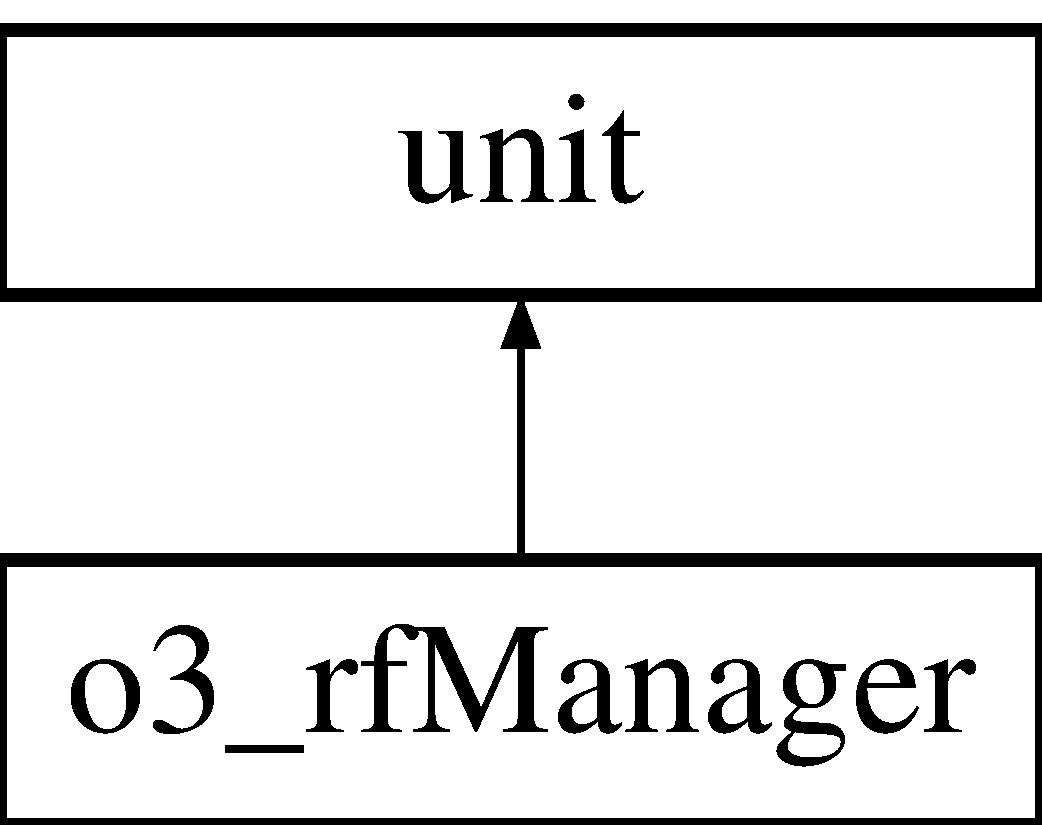
\includegraphics[height=2.000000cm]{classo3__rfManager}
\end{center}
\end{figure}
\subsection*{Public Member Functions}
\begin{DoxyCompactItemize}
\item 
\hyperlink{classo3__rfManager_a0abe0df5acbb3b9d1514b62d38647cff}{o3\_\-rfManager} (string rf\_\-name=\char`\"{}o3\_\-rfManager\char`\"{})
\item 
\hyperlink{classo3__rfManager_a42a66fc34794ca6c7209f743557a2b3a}{$\sim$o3\_\-rfManager} ()
\item 
bool \hyperlink{classo3__rfManager_a95bfea851bf8107f208e550839749063}{hasFreeWrPort} (\hyperlink{global_2global_8h_a7e19a550ec11d1ed921deb20c22efb5b}{CYCLE} now)
\item 
bool \hyperlink{classo3__rfManager_a0883b605da49fe18bf7a1a04219307ab}{hasFreeRdPort} (\hyperlink{global_2global_8h_a7e19a550ec11d1ed921deb20c22efb5b}{CYCLE} now, \hyperlink{global_2global_8h_a6fa2e24b8a418fa215e183264cbea3aa}{WIDTH} numRegRdPorts)
\item 
bool \hyperlink{classo3__rfManager_a023f3671f90123fe8749ff13606f273c}{canRename} (\hyperlink{classdynInstruction}{dynInstruction} $\ast$ins)
\item 
bool \hyperlink{classo3__rfManager_a702dcade81b3d2ccba4bae0ef8d7de30}{renameRegs} (\hyperlink{classdynInstruction}{dynInstruction} $\ast$ins)
\item 
bool \hyperlink{classo3__rfManager_a9b85902c553b147228d0bb3b57280ca7}{isReady} (\hyperlink{classdynInstruction}{dynInstruction} $\ast$ins)
\item 
void \hyperlink{classo3__rfManager_a06b8854ab37feb6b44166a8565dc447a}{completeRegs} (\hyperlink{classdynInstruction}{dynInstruction} $\ast$ins)
\item 
void \hyperlink{classo3__rfManager_a7d3aa6c1316bac1153b24b7764d301fb}{commitRegs} (\hyperlink{classdynInstruction}{dynInstruction} $\ast$ins)
\item 
void \hyperlink{classo3__rfManager_ac8199decc9c7a881b2099a68711cced7}{squashRenameReg} ()
\end{DoxyCompactItemize}


\subsection{Constructor \& Destructor Documentation}
\hypertarget{classo3__rfManager_a0abe0df5acbb3b9d1514b62d38647cff}{
\index{o3\_\-rfManager@{o3\_\-rfManager}!o3\_\-rfManager@{o3\_\-rfManager}}
\index{o3\_\-rfManager@{o3\_\-rfManager}!o3_rfManager@{o3\_\-rfManager}}
\subsubsection[{o3\_\-rfManager}]{\setlength{\rightskip}{0pt plus 5cm}o3\_\-rfManager::o3\_\-rfManager (
\begin{DoxyParamCaption}
\item[{string}]{rf\_\-name = {\ttfamily \char`\"{}o3\_\-rfManager\char`\"{}}}
\end{DoxyParamCaption}
)}}
\label{classo3__rfManager_a0abe0df5acbb3b9d1514b62d38647cff}

\begin{DoxyCode}
    : unit (rf_name),
      _GRF ("registerRename")
{ }
\end{DoxyCode}
\hypertarget{classo3__rfManager_a42a66fc34794ca6c7209f743557a2b3a}{
\index{o3\_\-rfManager@{o3\_\-rfManager}!$\sim$o3\_\-rfManager@{$\sim$o3\_\-rfManager}}
\index{$\sim$o3\_\-rfManager@{$\sim$o3\_\-rfManager}!o3_rfManager@{o3\_\-rfManager}}
\subsubsection[{$\sim$o3\_\-rfManager}]{\setlength{\rightskip}{0pt plus 5cm}o3\_\-rfManager::$\sim$o3\_\-rfManager (
\begin{DoxyParamCaption}
{}
\end{DoxyParamCaption}
)}}
\label{classo3__rfManager_a42a66fc34794ca6c7209f743557a2b3a}

\begin{DoxyCode}
{ }
\end{DoxyCode}


\subsection{Member Function Documentation}
\hypertarget{classo3__rfManager_a023f3671f90123fe8749ff13606f273c}{
\index{o3\_\-rfManager@{o3\_\-rfManager}!canRename@{canRename}}
\index{canRename@{canRename}!o3_rfManager@{o3\_\-rfManager}}
\subsubsection[{canRename}]{\setlength{\rightskip}{0pt plus 5cm}bool o3\_\-rfManager::canRename (
\begin{DoxyParamCaption}
\item[{{\bf dynInstruction} $\ast$}]{ins}
\end{DoxyParamCaption}
)}}
\label{classo3__rfManager_a023f3671f90123fe8749ff13606f273c}

\begin{DoxyCode}
                                                 {
    List<AR>* ar_wr = ins->getARwrList ();
    if (_GRF.getNumAvailablePR () < ar_wr->NumElements ()) {
        return false; /* STALL FETCH */
    }
    return true;
}
\end{DoxyCode}
\hypertarget{classo3__rfManager_a7d3aa6c1316bac1153b24b7764d301fb}{
\index{o3\_\-rfManager@{o3\_\-rfManager}!commitRegs@{commitRegs}}
\index{commitRegs@{commitRegs}!o3_rfManager@{o3\_\-rfManager}}
\subsubsection[{commitRegs}]{\setlength{\rightskip}{0pt plus 5cm}void o3\_\-rfManager::commitRegs (
\begin{DoxyParamCaption}
\item[{{\bf dynInstruction} $\ast$}]{ins}
\end{DoxyParamCaption}
)}}
\label{classo3__rfManager_a7d3aa6c1316bac1153b24b7764d301fb}

\begin{DoxyCode}
                                                  {
    List<PR>* _pr = ins->getPRwrList ();
    List<PR>* _ar = ins->getARwrList ();
    Assert (_ar->NumElements () == _pr->NumElements ());
    for (int i = 0; i < _pr->NumElements (); i++) {
        PR p_reg = _pr->Nth (i);
        AR a_reg = _ar->Nth (i);
        PR prev_pr = _GRF.getPrevPR (p_reg);
        _GRF.updatePRstate (p_reg,ARCH_REG);
        _GRF.updatePRstate (prev_pr,AVAILABLE);
        _GRF.update_cRAT (a_reg,p_reg);
        _GRF.setAsAvailablePR (prev_pr);
    }
}
\end{DoxyCode}
\hypertarget{classo3__rfManager_a06b8854ab37feb6b44166a8565dc447a}{
\index{o3\_\-rfManager@{o3\_\-rfManager}!completeRegs@{completeRegs}}
\index{completeRegs@{completeRegs}!o3_rfManager@{o3\_\-rfManager}}
\subsubsection[{completeRegs}]{\setlength{\rightskip}{0pt plus 5cm}void o3\_\-rfManager::completeRegs (
\begin{DoxyParamCaption}
\item[{{\bf dynInstruction} $\ast$}]{ins}
\end{DoxyParamCaption}
)}}
\label{classo3__rfManager_a06b8854ab37feb6b44166a8565dc447a}

\begin{DoxyCode}
                                                    {
    List<PR>* _pr = ins->getPRwrList ();
    for (int i = 0; i < _pr->NumElements (); i++) {
        PR p_reg = _pr->Nth (i);
        _GRF.updatePRstate (p_reg,RENAMED_VALID);
    }
}
\end{DoxyCode}
\hypertarget{classo3__rfManager_a0883b605da49fe18bf7a1a04219307ab}{
\index{o3\_\-rfManager@{o3\_\-rfManager}!hasFreeRdPort@{hasFreeRdPort}}
\index{hasFreeRdPort@{hasFreeRdPort}!o3_rfManager@{o3\_\-rfManager}}
\subsubsection[{hasFreeRdPort}]{\setlength{\rightskip}{0pt plus 5cm}bool o3\_\-rfManager::hasFreeRdPort (
\begin{DoxyParamCaption}
\item[{{\bf CYCLE}}]{now, }
\item[{{\bf WIDTH}}]{numRegRdPorts}
\end{DoxyParamCaption}
)}}
\label{classo3__rfManager_a0883b605da49fe18bf7a1a04219307ab}

\begin{DoxyCode}
                                                                {
    return _GRF.hasFreeRdPort (now, numRegRdPorts);
}
\end{DoxyCode}
\hypertarget{classo3__rfManager_a95bfea851bf8107f208e550839749063}{
\index{o3\_\-rfManager@{o3\_\-rfManager}!hasFreeWrPort@{hasFreeWrPort}}
\index{hasFreeWrPort@{hasFreeWrPort}!o3_rfManager@{o3\_\-rfManager}}
\subsubsection[{hasFreeWrPort}]{\setlength{\rightskip}{0pt plus 5cm}bool o3\_\-rfManager::hasFreeWrPort (
\begin{DoxyParamCaption}
\item[{{\bf CYCLE}}]{now}
\end{DoxyParamCaption}
)}}
\label{classo3__rfManager_a95bfea851bf8107f208e550839749063}

\begin{DoxyCode}
                                           {
    return _GRF.hasFreeWrPort (now);
}
\end{DoxyCode}
\hypertarget{classo3__rfManager_a9b85902c553b147228d0bb3b57280ca7}{
\index{o3\_\-rfManager@{o3\_\-rfManager}!isReady@{isReady}}
\index{isReady@{isReady}!o3_rfManager@{o3\_\-rfManager}}
\subsubsection[{isReady}]{\setlength{\rightskip}{0pt plus 5cm}bool o3\_\-rfManager::isReady (
\begin{DoxyParamCaption}
\item[{{\bf dynInstruction} $\ast$}]{ins}
\end{DoxyParamCaption}
)}}
\label{classo3__rfManager_a9b85902c553b147228d0bb3b57280ca7}

\begin{DoxyCode}
                                               {
    List<AR>* p_rdReg_list = ins->getPRrdList ();
    for (int i = p_rdReg_list->NumElements () - 1; i >= 0; i--) {
        AR reg = p_rdReg_list->Nth (i);
        if (!_GRF.isPRvalid (reg)) {
            return false; /* operand not available */
        } else {
            p_rdReg_list->RemoveAt (i); /*optimization */
        }
    }
    if (p_rdReg_list->NumElements () == 0) {
        return true; /* all operands available */
    }
    return false; /* not all operands available */
}
\end{DoxyCode}
\hypertarget{classo3__rfManager_a702dcade81b3d2ccba4bae0ef8d7de30}{
\index{o3\_\-rfManager@{o3\_\-rfManager}!renameRegs@{renameRegs}}
\index{renameRegs@{renameRegs}!o3_rfManager@{o3\_\-rfManager}}
\subsubsection[{renameRegs}]{\setlength{\rightskip}{0pt plus 5cm}bool o3\_\-rfManager::renameRegs (
\begin{DoxyParamCaption}
\item[{{\bf dynInstruction} $\ast$}]{ins}
\end{DoxyParamCaption}
)}}
\label{classo3__rfManager_a702dcade81b3d2ccba4bae0ef8d7de30}

\begin{DoxyCode}
                                                  {
    List<AR>* ar_rd = ins->getARrdList ();
    List<AR>* ar_wr = ins->getARwrList ();
    Assert (_GRF.getNumAvailablePR () >= ar_wr->NumElements ());

    /* RENAME READ REFISTERS FIRST */
    for (int i = 0; i < ar_rd->NumElements (); i++) {
        AR a_reg = ar_rd->Nth (i);
        PR p_reg = _GRF.renameReg (a_reg);
        ins->setPR (p_reg, READ);
    }

    /* RENAME WRITE REFISTERS SECOND */
    for (int i = 0; i < ar_wr->NumElements (); i++) {
        Assert (_GRF.isAnyPRavailable () == true && "A physical reg must have bee
      n available.");
        AR a_reg = ar_wr->Nth (i);
        PR prev_pr = _GRF.renameReg (a_reg);
        PR new_pr = _GRF.getAvailablePR ();
        _GRF.update_fRAT (a_reg, new_pr);
        _GRF.updatePR (new_pr, prev_pr, RENAMED_INVALID);
        ins->setPR (new_pr, WRITE);
    }
    return false; /* DON'T STALL FETCH */
}
\end{DoxyCode}
\hypertarget{classo3__rfManager_ac8199decc9c7a881b2099a68711cced7}{
\index{o3\_\-rfManager@{o3\_\-rfManager}!squashRenameReg@{squashRenameReg}}
\index{squashRenameReg@{squashRenameReg}!o3_rfManager@{o3\_\-rfManager}}
\subsubsection[{squashRenameReg}]{\setlength{\rightskip}{0pt plus 5cm}void o3\_\-rfManager::squashRenameReg (
\begin{DoxyParamCaption}
{}
\end{DoxyParamCaption}
)}}
\label{classo3__rfManager_ac8199decc9c7a881b2099a68711cced7}

\begin{DoxyCode}
                                    {
    dbg.print (DBG_TEST, "** %s: %s (cyc:)\n", _c_name.c_str (), "in squash for R
      R");
    _GRF.squashRenameReg ();
}
\end{DoxyCode}


The documentation for this class was generated from the following files:\begin{DoxyCompactItemize}
\item 
/home/milad/esc\_\-project/svn/PARS/src/backend/o3/\hyperlink{o3_2rfManager_8h}{rfManager.h}\item 
/home/milad/esc\_\-project/svn/PARS/src/backend/o3/\hyperlink{o3_2rfManager_8cpp}{rfManager.cpp}\end{DoxyCompactItemize}

\hypertarget{classo3__scheduler}{
\section{o3\_\-scheduler Class Reference}
\label{classo3__scheduler}\index{o3\_\-scheduler@{o3\_\-scheduler}}
}


{\ttfamily \#include $<$schedulers.h$>$}



Inheritance diagram for o3\_\-scheduler:


Collaboration diagram for o3\_\-scheduler:
\subsection*{Public Member Functions}
\begin{DoxyCompactItemize}
\item 
\hyperlink{classo3__scheduler_a5aa72000043c2ff5cf065160560da9be}{o3\_\-scheduler} (\hyperlink{classport}{port}$<$ \hyperlink{classdynInstruction}{dynInstruction} $\ast$ $>$ \&decode\_\-to\_\-scheduler\_\-port, \hyperlink{classport}{port}$<$ \hyperlink{classdynInstruction}{dynInstruction} $\ast$ $>$ \&execution\_\-to\_\-scheduler\_\-port, \hyperlink{classport}{port}$<$ \hyperlink{classdynInstruction}{dynInstruction} $\ast$ $>$ \&memory\_\-to\_\-scheduler\_\-port, \hyperlink{classport}{port}$<$ \hyperlink{classdynInstruction}{dynInstruction} $\ast$ $>$ \&scheduler\_\-to\_\-execution\_\-port, \hyperlink{classCAMtable}{CAMtable}$<$ \hyperlink{classdynInstruction}{dynInstruction} $\ast$ $>$ $\ast$\hyperlink{backend_2parser_8cpp_ad73ae25f81e6e99482f3fbd5ba9664ce}{iROB}, \hyperlink{global_2global_8h_a6fa2e24b8a418fa215e183264cbea3aa}{WIDTH} scheduler\_\-width, string stage\_\-name)
\item 
\hyperlink{classo3__scheduler_ad9624ab36caacb50f844098a32b1fa94}{$\sim$o3\_\-scheduler} ()
\item 
void \hyperlink{classo3__scheduler_a336443d7d6e8f6b892c7c71b97099e40}{doSCHEDULER} (\hyperlink{classsysClock}{sysClock} \&clk)
\item 
void \hyperlink{classo3__scheduler_a53e17bdeda48c023a7f24e6871eeed4c}{squash} (\hyperlink{classsysClock}{sysClock} \&clk)
\item 
\hyperlink{unit_2stage_8h_ab00e4188e8b8974fecb1dfd12764cbb1}{PIPE\_\-ACTIVITY} \hyperlink{classo3__scheduler_ade8fe27e00ac0430122634af01c0639c}{schedulerImpl} (\hyperlink{classsysClock}{sysClock} \&clk)
\item 
void \hyperlink{classo3__scheduler_a3eaa3373cbbd123523a9cbf4d7326692}{updateResStns} (\hyperlink{classsysClock}{sysClock} \&clk)
\item 
void \hyperlink{classo3__scheduler_a5dfd1ae3623b060e60867808e78b224a}{manageCDB} (\hyperlink{classsysClock}{sysClock} \&clk)
\item 
void \hyperlink{classo3__scheduler_a13b34d2dae20e349ee7bb614d0d33d46}{forwardFromCDB} (\hyperlink{classdynInstruction}{dynInstruction} $\ast$ins, \hyperlink{classsysClock}{sysClock} \&clk)
\item 
void \hyperlink{classo3__scheduler_a3ca0bc2505c006ce212a82f58b243e43}{regStat} (\hyperlink{classsysClock}{sysClock} \&clk)
\item 
bool \hyperlink{classo3__scheduler_a46d9cb288bfbd52069935fa96d9de38f}{hasReadyInsInResStn} (\hyperlink{global_2global_8h_a6fa2e24b8a418fa215e183264cbea3aa}{WIDTH} resStnId, \hyperlink{global_2global_8h_ad7ec63c69447a2b630929c8e0197860d}{LENGTH} \&readyInsIndx)
\end{DoxyCompactItemize}


\subsection{Constructor \& Destructor Documentation}
\hypertarget{classo3__scheduler_a5aa72000043c2ff5cf065160560da9be}{
\index{o3\_\-scheduler@{o3\_\-scheduler}!o3\_\-scheduler@{o3\_\-scheduler}}
\index{o3\_\-scheduler@{o3\_\-scheduler}!o3_scheduler@{o3\_\-scheduler}}
\subsubsection[{o3\_\-scheduler}]{\setlength{\rightskip}{0pt plus 5cm}o3\_\-scheduler::o3\_\-scheduler (
\begin{DoxyParamCaption}
\item[{{\bf port}$<$ {\bf dynInstruction} $\ast$ $>$ \&}]{decode\_\-to\_\-scheduler\_\-port, }
\item[{{\bf port}$<$ {\bf dynInstruction} $\ast$ $>$ \&}]{execution\_\-to\_\-scheduler\_\-port, }
\item[{{\bf port}$<$ {\bf dynInstruction} $\ast$ $>$ \&}]{memory\_\-to\_\-scheduler\_\-port, }
\item[{{\bf port}$<$ {\bf dynInstruction} $\ast$ $>$ \&}]{scheduler\_\-to\_\-execution\_\-port, }
\item[{{\bf CAMtable}$<$ {\bf dynInstruction} $\ast$ $>$ $\ast$}]{iROB, }
\item[{{\bf WIDTH}}]{scheduler\_\-width, }
\item[{string}]{stage\_\-name}
\end{DoxyParamCaption}
)}}
\label{classo3__scheduler_a5aa72000043c2ff5cf065160560da9be}

\begin{DoxyCode}
        : stage (issue_width, stage_name)
{
    _decode_to_scheduler_port = &decode_to_scheduler_port;
    _execution_to_scheduler_port = &execution_to_scheduler_port;
    _memory_to_scheduler_port = &memory_to_scheduler_port;
    _scheduler_to_execution_port  = &scheduler_to_execution_port;
    _iROB = iROB;
    _num_res_stns = 4;
    for (WIDTH i = 0; i < _num_res_stns; i++) {
        ostringstream rs_num;
        rs_num << i;
        CAMtable<dynInstruction*>* resStn = new CAMtable<dynInstruction*>(8, 8, 8
      , "ResStn_"+rs_num.str ());
        _ResStns.Append(resStn);
    }
}
\end{DoxyCode}


Here is the call graph for this function:


\hypertarget{classo3__scheduler_ad9624ab36caacb50f844098a32b1fa94}{
\index{o3\_\-scheduler@{o3\_\-scheduler}!$\sim$o3\_\-scheduler@{$\sim$o3\_\-scheduler}}
\index{$\sim$o3\_\-scheduler@{$\sim$o3\_\-scheduler}!o3_scheduler@{o3\_\-scheduler}}
\subsubsection[{$\sim$o3\_\-scheduler}]{\setlength{\rightskip}{0pt plus 5cm}o3\_\-scheduler::$\sim$o3\_\-scheduler (
\begin{DoxyParamCaption}
{}
\end{DoxyParamCaption}
)}}
\label{classo3__scheduler_ad9624ab36caacb50f844098a32b1fa94}

\begin{DoxyCode}
                             {
    for (WIDTH i = 0; i < _num_res_stns; i++) {
        delete _ResStns.Nth(i);
    }
}
\end{DoxyCode}


Here is the call graph for this function:




\subsection{Member Function Documentation}
\hypertarget{classo3__scheduler_a336443d7d6e8f6b892c7c71b97099e40}{
\index{o3\_\-scheduler@{o3\_\-scheduler}!doSCHEDULER@{doSCHEDULER}}
\index{doSCHEDULER@{doSCHEDULER}!o3_scheduler@{o3\_\-scheduler}}
\subsubsection[{doSCHEDULER}]{\setlength{\rightskip}{0pt plus 5cm}void o3\_\-scheduler::doSCHEDULER (
\begin{DoxyParamCaption}
\item[{{\bf sysClock} \&}]{clk}
\end{DoxyParamCaption}
)}}
\label{classo3__scheduler_a336443d7d6e8f6b892c7c71b97099e40}

\begin{DoxyCode}
                                             {
    /* STAT + DEBUG */
    dbg.print (DBG_SCHEDULER, "** %s: (cyc: %d)\n", _stage_name.c_str (), clk.
      now ());
    regStat (clk);
    PIPE_ACTIVITY pipe_stall = PIPE_STALL;

    /* SQUASH HANDLING */
    if (g_var.g_pipe_state == PIPE_FLUSH) { squash (clk); }
    if (!(g_var.g_pipe_state == PIPE_WAIT_FLUSH || g_var.g_pipe_state == 
      PIPE_FLUSH)) {
        pipe_stall = schedulerImpl (clk);
    }

    /* STAT */
    if (pipe_stall == PIPE_STALL) s_stall_cycles++;
}
\end{DoxyCode}


Here is the call graph for this function:




Here is the caller graph for this function:


\hypertarget{classo3__scheduler_a13b34d2dae20e349ee7bb614d0d33d46}{
\index{o3\_\-scheduler@{o3\_\-scheduler}!forwardFromCDB@{forwardFromCDB}}
\index{forwardFromCDB@{forwardFromCDB}!o3_scheduler@{o3\_\-scheduler}}
\subsubsection[{forwardFromCDB}]{\setlength{\rightskip}{0pt plus 5cm}void o3\_\-scheduler::forwardFromCDB (
\begin{DoxyParamCaption}
\item[{{\bf dynInstruction} $\ast$}]{ins, }
\item[{{\bf sysClock} \&}]{clk}
\end{DoxyParamCaption}
)}}
\label{classo3__scheduler_a13b34d2dae20e349ee7bb614d0d33d46}

\begin{DoxyCode}
                                                                     {
    { /* FWD FROM EXE STAGE */
        if (_execution_to_scheduler_port->getBuffState (clk.now ()) == 
      EMPTY_BUFF) return;
        List<PR>* rd_reg_list = ins->getPRrdList ();
        List<dynInstruction*> fwd_list;
        for (WIDTH i = 0; i < _stage_width; i++) { //TODO _stage_width replace wi
      th exe_num_EU
            if (!_execution_to_scheduler_port->isReadyNow (clk.now ())) break;
            dynInstruction* fwd_ins = _execution_to_scheduler_port->popFront (clk
      .now ());
            fwd_list.Append (fwd_ins);
        }
        for (WIDTH i = 0; i < fwd_list.NumElements (); i++) {
            dynInstruction* fwd_ins = fwd_list.Nth (i);
            List<PR>* wr_reg_list = fwd_ins->getPRwrList ();
            for (int j = rd_reg_list->NumElements () - 1; j >= 0; j--) {
                PR rd_reg = rd_reg_list->Nth (j);
                for (int k = wr_reg_list->NumElements () - 1; k >= 0; k--) {
                    PR wr_reg = wr_reg_list->Nth (k);
                    if (rd_reg == wr_reg) {
                        rd_reg_list->RemoveAt(j);
                    }
                }
            }
        }
        _execution_to_scheduler_port->delOldReady (clk.now ()); /* Only FWD what 
      is on CDB now */
    }

    { /* FWD FROM MEM STAGE */
        if (_memory_to_scheduler_port->getBuffState (clk.now ()) == EMPTY_BUFF) r
      eturn;
        List<PR>* rd_reg_list = ins->getPRrdList ();
        List<dynInstruction*> fwd_list;
        for (WIDTH i = 0; i < _stage_width; i++) { //TODO _stage_width replace wi
      th exe_num_EU
            if (!_memory_to_scheduler_port->hasReadyNow (clk.now ())) break;
            dynInstruction* fwd_ins = _memory_to_scheduler_port->popNextReadyNow 
      (clk.now ());
            fwd_list.Append (fwd_ins);
        }
        for (WIDTH i = 0; i < fwd_list.NumElements (); i++) {
            dynInstruction* fwd_ins = fwd_list.Nth (i);
            List<PR>* wr_reg_list = fwd_ins->getPRwrList ();
            for (int j = rd_reg_list->NumElements () - 1; j >= 0; j--) {
                PR rd_reg = rd_reg_list->Nth (j);
                for (int k = wr_reg_list->NumElements () - 1; k >= 0; k--) {
                    PR wr_reg = wr_reg_list->Nth (k);
                    if (rd_reg == wr_reg) {
                        rd_reg_list->RemoveAt(j);
                    }
                }
            }
        }
        _memory_to_scheduler_port->delOldReady (clk.now ()); /* Only FWD what is 
      on CDB now */
    }
}
\end{DoxyCode}


Here is the call graph for this function:


\hypertarget{classo3__scheduler_a46d9cb288bfbd52069935fa96d9de38f}{
\index{o3\_\-scheduler@{o3\_\-scheduler}!hasReadyInsInResStn@{hasReadyInsInResStn}}
\index{hasReadyInsInResStn@{hasReadyInsInResStn}!o3_scheduler@{o3\_\-scheduler}}
\subsubsection[{hasReadyInsInResStn}]{\setlength{\rightskip}{0pt plus 5cm}bool o3\_\-scheduler::hasReadyInsInResStn (
\begin{DoxyParamCaption}
\item[{{\bf WIDTH}}]{resStnId, }
\item[{{\bf LENGTH} \&}]{readyInsIndx}
\end{DoxyParamCaption}
)}}
\label{classo3__scheduler_a46d9cb288bfbd52069935fa96d9de38f}

\begin{DoxyCode}
                                                                            {
    for (WIDTH i = 0; i < _ResStns.Nth(resStnId)->getTableSize(); i++) {
        dynInstruction* ins = _ResStns.Nth(resStnId)->getNth_unsafe (i);
        readyInsIndx = i;
        if (!g_GRF_MGR.isReady (ins)) continue;
        else return true;
    }
    return false;
}
\end{DoxyCode}


Here is the call graph for this function:




Here is the caller graph for this function:


\hypertarget{classo3__scheduler_a5dfd1ae3623b060e60867808e78b224a}{
\index{o3\_\-scheduler@{o3\_\-scheduler}!manageCDB@{manageCDB}}
\index{manageCDB@{manageCDB}!o3_scheduler@{o3\_\-scheduler}}
\subsubsection[{manageCDB}]{\setlength{\rightskip}{0pt plus 5cm}void o3\_\-scheduler::manageCDB (
\begin{DoxyParamCaption}
\item[{{\bf sysClock} \&}]{clk}
\end{DoxyParamCaption}
)}}
\label{classo3__scheduler_a5dfd1ae3623b060e60867808e78b224a}

\begin{DoxyCode}
                                           {
    if (_execution_to_scheduler_port->getBuffState (clk.now ()) == EMPTY_BUFF) re
      turn;
    for (WIDTH i = 0; i < _stage_width; i++) { //TODO _stage_width replace with e
      xe_num_EU
        if (_execution_to_scheduler_port->isReady (clk.now ()))
            _execution_to_scheduler_port->popFront (clk.now ());
    }
}
\end{DoxyCode}


Here is the call graph for this function:




Here is the caller graph for this function:


\hypertarget{classo3__scheduler_a3ca0bc2505c006ce212a82f58b243e43}{
\index{o3\_\-scheduler@{o3\_\-scheduler}!regStat@{regStat}}
\index{regStat@{regStat}!o3_scheduler@{o3\_\-scheduler}}
\subsubsection[{regStat}]{\setlength{\rightskip}{0pt plus 5cm}void o3\_\-scheduler::regStat (
\begin{DoxyParamCaption}
\item[{{\bf sysClock} \&}]{clk}
\end{DoxyParamCaption}
)}}
\label{classo3__scheduler_a3ca0bc2505c006ce212a82f58b243e43}

\begin{DoxyCode}
                                         {
    _decode_to_scheduler_port->regStat (clk.now ());
    _execution_to_scheduler_port->regStat (clk.now ());
    _memory_to_scheduler_port->regStat (clk.now ());
    for (WIDTH j = 0; j < _num_res_stns; j++) {
        _ResStns.Nth(j)->regStat ();
    }
}
\end{DoxyCode}


Here is the call graph for this function:




Here is the caller graph for this function:


\hypertarget{classo3__scheduler_ade8fe27e00ac0430122634af01c0639c}{
\index{o3\_\-scheduler@{o3\_\-scheduler}!schedulerImpl@{schedulerImpl}}
\index{schedulerImpl@{schedulerImpl}!o3_scheduler@{o3\_\-scheduler}}
\subsubsection[{schedulerImpl}]{\setlength{\rightskip}{0pt plus 5cm}{\bf PIPE\_\-ACTIVITY} o3\_\-scheduler::schedulerImpl (
\begin{DoxyParamCaption}
\item[{{\bf sysClock} \&}]{clk}
\end{DoxyParamCaption}
)}}
\label{classo3__scheduler_ade8fe27e00ac0430122634af01c0639c}

\begin{DoxyCode}
                                                        {
    PIPE_ACTIVITY pipe_stall = PIPE_STALL;

    updateResStns (clk);

    /* READ FROM INS WINDOW */
    for (WIDTH j = 0; j < _num_res_stns; j++) {
        for (WIDTH i = 0; i < _stage_width; i++) {
            /* CHECKS */
            if (_scheduler_to_execution_port->getBuffState (clk.now ()) == 
      FULL_BUFF) break;
            if (_ResStns.Nth(j)->getTableState () == EMPTY_BUFF) continue;
            if (!_ResStns.Nth(j)->hasFreeRdPort (clk.now ())) continue;
            LENGTH readyInsIndx;
            if (!hasReadyInsInResStn (j, readyInsIndx)) break;
            dynInstruction* ins = _ResStns.Nth(j)->getNth_unsafe (readyInsIndx);
            if (!g_GRF_MGR.hasFreeRdPort (clk.now (), ins->getNumRdPR ())) break;
      
            //forwardFromCDB (ins, clk); TODO - made execution worse - WHY?!

            /* READ INS WIN */
            ins = _ResStns.Nth(j)->pullNextReady (readyInsIndx);
            ins->setPipeStage (ISSUE);
            _scheduler_to_execution_port->pushBack (ins, clk.now ());
            dbg.print (DBG_SCHEDULER, "%s: %s %llu (cyc: %d)\n", _stage_name.c_st
      r (), "Issue ins", ins->getInsID (), clk.now ());

            /* STAT */
            s_ins_cnt++;
            pipe_stall = PIPE_BUSY;
        }
    }

    manageCDB (clk);

    return pipe_stall;
}
\end{DoxyCode}


Here is the call graph for this function:




Here is the caller graph for this function:


\hypertarget{classo3__scheduler_a53e17bdeda48c023a7f24e6871eeed4c}{
\index{o3\_\-scheduler@{o3\_\-scheduler}!squash@{squash}}
\index{squash@{squash}!o3_scheduler@{o3\_\-scheduler}}
\subsubsection[{squash}]{\setlength{\rightskip}{0pt plus 5cm}void o3\_\-scheduler::squash (
\begin{DoxyParamCaption}
\item[{{\bf sysClock} \&}]{clk}
\end{DoxyParamCaption}
)}}
\label{classo3__scheduler_a53e17bdeda48c023a7f24e6871eeed4c}

\begin{DoxyCode}
                                        {
    dbg.print (DBG_SQUASH, "%s: %s (cyc: %d)\n", _stage_name.c_str (), "Scheduler
       Ports Flush", clk.now ());
    Assert (g_var.g_pipe_state == PIPE_FLUSH);
    INS_ID squashSeqNum = g_var.getSquashSN ();
    _scheduler_to_execution_port->flushPort (squashSeqNum, clk.now ());
    for (WIDTH j = 0; j < _num_res_stns; j++) {
        for (int i = (int)_ResStns.Nth(j)->getTableSize() - 1; i >= 0; i--) {
            if (_ResStns.Nth(j)->getTableSize() == 0) break;
            dynInstruction* ins = _ResStns.Nth(j)->getNth_unsafe (i);
            if (ins->getInsID () >= squashSeqNum) {
                _ResStns.Nth(j)->removeNth_unsafe (i);
            }
        }
    }
}
\end{DoxyCode}


Here is the call graph for this function:




Here is the caller graph for this function:


\hypertarget{classo3__scheduler_a3eaa3373cbbd123523a9cbf4d7326692}{
\index{o3\_\-scheduler@{o3\_\-scheduler}!updateResStns@{updateResStns}}
\index{updateResStns@{updateResStns}!o3_scheduler@{o3\_\-scheduler}}
\subsubsection[{updateResStns}]{\setlength{\rightskip}{0pt plus 5cm}void o3\_\-scheduler::updateResStns (
\begin{DoxyParamCaption}
\item[{{\bf sysClock} \&}]{clk}
\end{DoxyParamCaption}
)}}
\label{classo3__scheduler_a3eaa3373cbbd123523a9cbf4d7326692}

\begin{DoxyCode}
                                               {
    for (WIDTH j = 0; j < _num_res_stns; j++) {
        for (WIDTH i = 0; i < _stage_width; i++) {
            /* CHECKS */
            if (_iROB->getTableState () == FULL_BUFF) break;
            if (!_iROB->hasFreeWrPort (clk.now ())) break;
            if (_ResStns.Nth(j)->getTableState () == FULL_BUFF) continue;
            if (!_ResStns.Nth(j)->hasFreeWrPort (clk.now ())) continue;
            if (_decode_to_scheduler_port->getBuffState (clk.now ()) == 
      EMPTY_BUFF) break;
            if (!_decode_to_scheduler_port->isReady (clk.now ())) break;
            dynInstruction* ins = _decode_to_scheduler_port->getFront ();
            if (!g_GRF_MGR.canRename (ins)) break;
            if (ins->getInsType () == MEM && ins->getMemType () == LOAD) {
                if (g_LSQ_MGR.getTableState (LD_QU) == FULL_BUFF) break;
                if (!g_LSQ_MGR.hasFreeWrPort (LD_QU, clk.now ())) break;
            } else if (ins->getInsType () == MEM && ins->getMemType () == STORE) 
      {
                if (g_LSQ_MGR.getTableState (ST_QU) == FULL_BUFF) break;
                if (!g_LSQ_MGR.hasFreeWrPort (ST_QU, clk.now ())) break;
            }

            /* WRITE INTO RES STN */
            dbg.print (DBG_PORT, "%s: %s (cyc: %d)\n", _stage_name.c_str (), "ADD
       INS", clk.now ());
            ins = _decode_to_scheduler_port->popFront (clk.now ());
            g_GRF_MGR.renameRegs (ins);
            ins->setPipeStage (DISPATCH);
            if (ins->getInsType () == MEM) g_LSQ_MGR.pushBack (ins);
            _ResStns.Nth(j)->pushBack (ins);
            _iROB->pushBack (ins);
            dbg.print (DBG_SCHEDULER, "%s: %s %llu (cyc: %d)\n", _stage_name.c_st
      r (), "Write iWin ins", ins->getInsID (), clk.now ());
        }
    }
}
\end{DoxyCode}


Here is the call graph for this function:




Here is the caller graph for this function:




The documentation for this class was generated from the following files:\begin{DoxyCompactItemize}
\item 
/home/milad/esc\_\-project/svn/PARS/src/backend/o3/\hyperlink{o3_2schedulers_8h}{schedulers.h}\item 
/home/milad/esc\_\-project/svn/PARS/src/backend/o3/\hyperlink{o3_2schedulers_8cpp}{schedulers.cpp}\end{DoxyCompactItemize}

\hypertarget{classo3__sysCore}{
\section{o3\_\-sysCore Class Reference}
\label{classo3__sysCore}\index{o3\_\-sysCore@{o3\_\-sysCore}}
}


{\ttfamily \#include $<$sysCore.h$>$}



Inheritance diagram for o3\_\-sysCore:


Collaboration diagram for o3\_\-sysCore:
\subsection*{Public Member Functions}
\begin{DoxyCompactItemize}
\item 
\hyperlink{classo3__sysCore_aa2fc24a24dd599ff3393c62910cbcb06}{o3\_\-sysCore} (\hyperlink{global_2global_8h_a32516e1b668a88eb546e9b6ee2e3345d}{GHz} clk\_\-frequency, \hyperlink{global_2global_8h_a6fa2e24b8a418fa215e183264cbea3aa}{WIDTH} bp\_\-width, \hyperlink{global_2global_8h_a6fa2e24b8a418fa215e183264cbea3aa}{WIDTH} fetch\_\-width, \hyperlink{global_2global_8h_a6fa2e24b8a418fa215e183264cbea3aa}{WIDTH} decode\_\-width, \hyperlink{global_2global_8h_a6fa2e24b8a418fa215e183264cbea3aa}{WIDTH} scheduler\_\-width, \hyperlink{global_2global_8h_a6fa2e24b8a418fa215e183264cbea3aa}{WIDTH} execution\_\-width, \hyperlink{global_2global_8h_a6fa2e24b8a418fa215e183264cbea3aa}{WIDTH} memory\_\-width, \hyperlink{global_2global_8h_a6fa2e24b8a418fa215e183264cbea3aa}{WIDTH} commit\_\-width, \hyperlink{global_2global_8h_a7e19a550ec11d1ed921deb20c22efb5b}{CYCLE} fetch\_\-to\_\-decode\_\-delay, \hyperlink{global_2global_8h_ad7ec63c69447a2b630929c8e0197860d}{LENGTH} fetch\_\-to\_\-decode\_\-buff\_\-len, \hyperlink{global_2global_8h_a7e19a550ec11d1ed921deb20c22efb5b}{CYCLE} fetch\_\-to\_\-bp\_\-delay, \hyperlink{global_2global_8h_ad7ec63c69447a2b630929c8e0197860d}{LENGTH} fetch\_\-to\_\-bp\_\-buff\_\-len, \hyperlink{global_2global_8h_a7e19a550ec11d1ed921deb20c22efb5b}{CYCLE} bp\_\-to\_\-fetch\_\-delay, \hyperlink{global_2global_8h_ad7ec63c69447a2b630929c8e0197860d}{LENGTH} bp\_\-to\_\-fetch\_\-buff\_\-len, \hyperlink{global_2global_8h_a7e19a550ec11d1ed921deb20c22efb5b}{CYCLE} decode\_\-to\_\-scheduler\_\-delay, \hyperlink{global_2global_8h_ad7ec63c69447a2b630929c8e0197860d}{LENGTH} decode\_\-to\_\-scheduler\_\-buff\_\-len, \hyperlink{global_2global_8h_a7e19a550ec11d1ed921deb20c22efb5b}{CYCLE} scheduler\_\-to\_\-execution\_\-delay, \hyperlink{global_2global_8h_ad7ec63c69447a2b630929c8e0197860d}{LENGTH} scheduler\_\-to\_\-execution\_\-buff\_\-len, \hyperlink{global_2global_8h_a7e19a550ec11d1ed921deb20c22efb5b}{CYCLE} execution\_\-to\_\-scheduler\_\-delay, \hyperlink{global_2global_8h_ad7ec63c69447a2b630929c8e0197860d}{LENGTH} execution\_\-to\_\-scheduler\_\-buff\_\-len, \hyperlink{global_2global_8h_a7e19a550ec11d1ed921deb20c22efb5b}{CYCLE} execution\_\-to\_\-memory\_\-delay, \hyperlink{global_2global_8h_ad7ec63c69447a2b630929c8e0197860d}{LENGTH} execution\_\-to\_\-memory\_\-buff\_\-len, \hyperlink{global_2global_8h_a7e19a550ec11d1ed921deb20c22efb5b}{CYCLE} memory\_\-to\_\-scheduler\_\-delay, \hyperlink{global_2global_8h_ad7ec63c69447a2b630929c8e0197860d}{LENGTH} memory\_\-to\_\-scheduler\_\-buff\_\-len, \hyperlink{global_2global_8h_a7e19a550ec11d1ed921deb20c22efb5b}{CYCLE} commit\_\-to\_\-bp\_\-delay, \hyperlink{global_2global_8h_ad7ec63c69447a2b630929c8e0197860d}{LENGTH} commit\_\-to\_\-bp\_\-buff\_\-len, \hyperlink{global_2global_8h_a7e19a550ec11d1ed921deb20c22efb5b}{CYCLE} commit\_\-to\_\-scheduler\_\-delay, \hyperlink{global_2global_8h_ad7ec63c69447a2b630929c8e0197860d}{LENGTH} commit\_\-to\_\-scheduler\_\-buff\_\-len)
\item 
\hyperlink{classo3__sysCore_af4d8e609d9501b5511b70fbdfa218772}{$\sim$o3\_\-sysCore} ()
\item 
void \hyperlink{classo3__sysCore_ab97edaa7f8ea74d7315b71d7d03a736c}{runCore} ()
\end{DoxyCompactItemize}


\subsection{Constructor \& Destructor Documentation}
\hypertarget{classo3__sysCore_aa2fc24a24dd599ff3393c62910cbcb06}{
\index{o3\_\-sysCore@{o3\_\-sysCore}!o3\_\-sysCore@{o3\_\-sysCore}}
\index{o3\_\-sysCore@{o3\_\-sysCore}!o3_sysCore@{o3\_\-sysCore}}
\subsubsection[{o3\_\-sysCore}]{\setlength{\rightskip}{0pt plus 5cm}o3\_\-sysCore::o3\_\-sysCore (
\begin{DoxyParamCaption}
\item[{{\bf GHz}}]{clk\_\-frequency, }
\item[{{\bf WIDTH}}]{bp\_\-width, }
\item[{{\bf WIDTH}}]{fetch\_\-width, }
\item[{{\bf WIDTH}}]{decode\_\-width, }
\item[{{\bf WIDTH}}]{scheduler\_\-width, }
\item[{{\bf WIDTH}}]{execution\_\-width, }
\item[{{\bf WIDTH}}]{memory\_\-width, }
\item[{{\bf WIDTH}}]{commit\_\-width, }
\item[{{\bf CYCLE}}]{fetch\_\-to\_\-decode\_\-delay, }
\item[{{\bf LENGTH}}]{fetch\_\-to\_\-decode\_\-buff\_\-len, }
\item[{{\bf CYCLE}}]{fetch\_\-to\_\-bp\_\-delay, }
\item[{{\bf LENGTH}}]{fetch\_\-to\_\-bp\_\-buff\_\-len, }
\item[{{\bf CYCLE}}]{bp\_\-to\_\-fetch\_\-delay, }
\item[{{\bf LENGTH}}]{bp\_\-to\_\-fetch\_\-buff\_\-len, }
\item[{{\bf CYCLE}}]{decode\_\-to\_\-scheduler\_\-delay, }
\item[{{\bf LENGTH}}]{decode\_\-to\_\-scheduler\_\-buff\_\-len, }
\item[{{\bf CYCLE}}]{scheduler\_\-to\_\-execution\_\-delay, }
\item[{{\bf LENGTH}}]{scheduler\_\-to\_\-execution\_\-buff\_\-len, }
\item[{{\bf CYCLE}}]{execution\_\-to\_\-scheduler\_\-delay, }
\item[{{\bf LENGTH}}]{execution\_\-to\_\-scheduler\_\-buff\_\-len, }
\item[{{\bf CYCLE}}]{execution\_\-to\_\-memory\_\-delay, }
\item[{{\bf LENGTH}}]{execution\_\-to\_\-memory\_\-buff\_\-len, }
\item[{{\bf CYCLE}}]{memory\_\-to\_\-scheduler\_\-delay, }
\item[{{\bf LENGTH}}]{memory\_\-to\_\-scheduler\_\-buff\_\-len, }
\item[{{\bf CYCLE}}]{commit\_\-to\_\-bp\_\-delay, }
\item[{{\bf LENGTH}}]{commit\_\-to\_\-bp\_\-buff\_\-len, }
\item[{{\bf CYCLE}}]{commit\_\-to\_\-scheduler\_\-delay, }
\item[{{\bf LENGTH}}]{commit\_\-to\_\-scheduler\_\-buff\_\-len}
\end{DoxyParamCaption}
)}}
\label{classo3__sysCore_aa2fc24a24dd599ff3393c62910cbcb06}

\begin{DoxyCode}
        : unit("SysCore"),
      _fetch_to_decode_delay (fetch_to_decode_delay),
          _fetch_to_decode_buff_len (fetch_to_decode_buff_len),
          _fetch_to_bp_delay (fetch_to_bp_delay),
          _fetch_to_bp_buff_len (fetch_to_bp_buff_len),
          _bp_to_fetch_delay (bp_to_fetch_delay),
          _bp_to_fetch_buff_len (bp_to_fetch_buff_len),
          _decode_to_scheduler_delay (decode_to_scheduler_delay),
          _decode_to_scheduler_buff_len (decode_to_scheduler_buff_len),
          _scheduler_to_execution_delay (scheduler_to_execution_delay),
          _scheduler_to_execution_buff_len (scheduler_to_execution_buff_len),
          _execution_to_scheduler_delay (execution_to_scheduler_delay),
          _execution_to_scheduler_buff_len (execution_to_scheduler_buff_len),
          _execution_to_memory_delay (execution_to_memory_delay),
          _execution_to_memory_buff_len (execution_to_memory_buff_len),
          _memory_to_scheduler_delay (memory_to_scheduler_delay),
          _memory_to_scheduler_buff_len (memory_to_scheduler_buff_len),
          _commit_to_bp_delay (commit_to_bp_delay),
          _commit_to_bp_buff_len (commit_to_bp_buff_len),
          _commit_to_scheduler_delay (commit_to_scheduler_delay),
          _commit_to_scheduler_buff_len (commit_to_scheduler_buff_len),
      // INIT PORTS
      _bp_to_fetch_port (bp_to_fetch_buff_len, bp_to_fetch_delay, "bp_to_fetch_po
      rt"),
      _fetch_to_bp_port (fetch_to_bp_buff_len, fetch_to_bp_delay, "fetch_to_bp_po
      rt"),
      _fetch_to_decode_port (fetch_to_decode_buff_len, fetch_to_decode_delay, "fe
      tch_to_decode_port"),
      _decode_to_scheduler_port (decode_to_scheduler_buff_len, decode_to_schedule
      r_delay, "decode_to_scheduler_port"),
      _scheduler_to_execution_port (scheduler_to_execution_buff_len, scheduler_to
      _execution_delay, "scheduler_to_execution_port"),
      _execution_to_scheduler_port (execution_to_scheduler_buff_len, execution_to
      _scheduler_delay, "execution_to_scheduler_port"),
      _execution_to_memory_port (execution_to_memory_buff_len, execution_to_memor
      y_delay, "execution_to_memory_port"),
      _memory_to_scheduler_port (memory_to_scheduler_buff_len, memory_to_schedule
      r_delay, "memory_to_scheduler_port"),
      _commit_to_bp_port (commit_to_bp_buff_len, commit_to_bp_delay, "commit_to_b
      p_port"),
      _commit_to_scheduler_port (commit_to_scheduler_buff_len, commit_to_schedule
      r_delay, "commit_to_scheduler_port"),
          _clk (clk_frequency)
{
    _iROB = new CAMtable<dynInstruction*>(100, 32, 32, "iROB");
    // INIT STAGES
    dbg.print (DBG_CORE, "%s: Constructing CPU Stages", _c_name.c_str ());
    _bp = new o3_branchPred (_fetch_to_bp_port, _bp_to_fetch_port, bp_width, "bra
      nchPred");
    _fetch = new o3_fetch (_bp_to_fetch_port, _fetch_to_decode_port, _fetch_to_bp
      _port, fetch_width, "fetch");
    _decode = new o3_decode (_fetch_to_decode_port, _decode_to_scheduler_port, de
      code_width, "decode");
    _scheduler = new o3_scheduler (_decode_to_scheduler_port, _execution_to_sched
      uler_port, _memory_to_scheduler_port, _scheduler_to_execution_port, _iROB, schedu
      ler_width, "schedule");
    _execution = new o3_execution (_scheduler_to_execution_port, _execution_to_sc
      heduler_port, _execution_to_memory_port, _iROB, execution_width, "execution");
    _memory = new o3_memory (_execution_to_memory_port, _memory_to_scheduler_port
      , _iROB, memory_width, "memory");
    _commit = new o3_commit (_commit_to_bp_port, _commit_to_scheduler_port, _iROB
      , commit_width, "commit");
}
\end{DoxyCode}


Here is the call graph for this function:


\hypertarget{classo3__sysCore_af4d8e609d9501b5511b70fbdfa218772}{
\index{o3\_\-sysCore@{o3\_\-sysCore}!$\sim$o3\_\-sysCore@{$\sim$o3\_\-sysCore}}
\index{$\sim$o3\_\-sysCore@{$\sim$o3\_\-sysCore}!o3_sysCore@{o3\_\-sysCore}}
\subsubsection[{$\sim$o3\_\-sysCore}]{\setlength{\rightskip}{0pt plus 5cm}o3\_\-sysCore::$\sim$o3\_\-sysCore (
\begin{DoxyParamCaption}
{}
\end{DoxyParamCaption}
)}}
\label{classo3__sysCore_af4d8e609d9501b5511b70fbdfa218772}

\begin{DoxyCode}
                         {
    delete _iROB;
    delete _bp;
    delete _fetch;
    delete _decode;
    delete _scheduler;
    delete _execution;
}
\end{DoxyCode}


\subsection{Member Function Documentation}
\hypertarget{classo3__sysCore_ab97edaa7f8ea74d7315b71d7d03a736c}{
\index{o3\_\-sysCore@{o3\_\-sysCore}!runCore@{runCore}}
\index{runCore@{runCore}!o3_sysCore@{o3\_\-sysCore}}
\subsubsection[{runCore}]{\setlength{\rightskip}{0pt plus 5cm}void o3\_\-sysCore::runCore (
\begin{DoxyParamCaption}
{}
\end{DoxyParamCaption}
)}}
\label{classo3__sysCore_ab97edaa7f8ea74d7315b71d7d03a736c}

\begin{DoxyCode}
                          {
        while (true) {
                _clk.tick ();
        dbg.print (DBG_PORT, "\n** CYCLE %d **\n", _clk.now ());
            _commit->doCOMMIT (_clk);
            _memory->doMEMORY (_clk);
            _execution->doEXECUTION (_clk);
        if (g_var.g_pipe_state == PIPE_SQUASH_ROB) _commit->squash (_clk);
            _scheduler->doSCHEDULER (_clk);
            _decode->doDECODE (_clk);
            if (_fetch->doFETCH (_clk) == FRONT_END && g_var.g_pipe_state == 
      PIPE_NORMAL) {
            dbg.print (DBG_CORE, "SWITCH TO FRONTEND\n");
            break;
        }
        _bp->doBP (_clk);
        //if (_clk.now () == 1000) exit (-1);
        }
}
\end{DoxyCode}


Here is the call graph for this function:




Here is the caller graph for this function:




The documentation for this class was generated from the following files:\begin{DoxyCompactItemize}
\item 
/home/milad/esc\_\-project/svn/PARS/src/backend/o3/\hyperlink{o3_2sysCore_8h}{sysCore.h}\item 
/home/milad/esc\_\-project/svn/PARS/src/backend/o3/\hyperlink{o3_2sysCore_8cpp}{sysCore.cpp}\end{DoxyCompactItemize}

\hypertarget{structOPTR}{
\section{OPTR Struct Reference}
\label{structOPTR}\index{OPTR@{OPTR}}
}


{\ttfamily \#include $<$coff\_\-sym.h$>$}



Collaboration diagram for OPTR:
\subsection*{Public Attributes}
\begin{DoxyCompactItemize}
\item 
unsigned \hyperlink{structOPTR_a395372ba2e7eb725906f228749c39dd5}{ot}: 8
\item 
unsigned \hyperlink{structOPTR_a6539af4ff0b28e701633de620abfabbe}{value}: 24
\item 
\hyperlink{structRNDXR}{RNDXR} \hyperlink{structOPTR_a3894af1c17210c3c3e33577ef34161fa}{rndx}
\item 
coff\_\-ulong \hyperlink{structOPTR_af59ba1a417a747c35426cb6edd3c3a7a}{offset}
\end{DoxyCompactItemize}


\subsection{Member Data Documentation}
\hypertarget{structOPTR_af59ba1a417a747c35426cb6edd3c3a7a}{
\index{OPTR@{OPTR}!offset@{offset}}
\index{offset@{offset}!OPTR@{OPTR}}
\subsubsection[{offset}]{\setlength{\rightskip}{0pt plus 5cm}coff\_\-ulong {\bf OPTR::offset}}}
\label{structOPTR_af59ba1a417a747c35426cb6edd3c3a7a}
\hypertarget{structOPTR_a395372ba2e7eb725906f228749c39dd5}{
\index{OPTR@{OPTR}!ot@{ot}}
\index{ot@{ot}!OPTR@{OPTR}}
\subsubsection[{ot}]{\setlength{\rightskip}{0pt plus 5cm}unsigned {\bf OPTR::ot}}}
\label{structOPTR_a395372ba2e7eb725906f228749c39dd5}
\hypertarget{structOPTR_a3894af1c17210c3c3e33577ef34161fa}{
\index{OPTR@{OPTR}!rndx@{rndx}}
\index{rndx@{rndx}!OPTR@{OPTR}}
\subsubsection[{rndx}]{\setlength{\rightskip}{0pt plus 5cm}{\bf RNDXR} {\bf OPTR::rndx}}}
\label{structOPTR_a3894af1c17210c3c3e33577ef34161fa}
\hypertarget{structOPTR_a6539af4ff0b28e701633de620abfabbe}{
\index{OPTR@{OPTR}!value@{value}}
\index{value@{value}!OPTR@{OPTR}}
\subsubsection[{value}]{\setlength{\rightskip}{0pt plus 5cm}unsigned {\bf OPTR::value}}}
\label{structOPTR_a6539af4ff0b28e701633de620abfabbe}


The documentation for this struct was generated from the following file:\begin{DoxyCompactItemize}
\item 
/home/milad/esc\_\-project/svn/PARS/src/frontend/lib/bp\_\-lib/loader/\hyperlink{coff__sym_8h}{coff\_\-sym.h}\end{DoxyCompactItemize}

\input{classYAML_1_1ostream}
\input{structpackage__config__t__st}
\input{structpackage__RC__t__st}
\input{structPager}
\input{structPagerSavepoint}
\input{structParse}
\input{classYAML_1_1Parser}
\input{classYAML_1_1ParserException}
\input{structYAML_1_1ParserState}
\input{structPCache}
\input{structPCache1}
\hypertarget{structpdr}{
\section{pdr Struct Reference}
\label{structpdr}\index{pdr@{pdr}}
}


{\ttfamily \#include $<$coff\_\-sym.h$>$}

\subsection*{Public Attributes}
\begin{DoxyCompactItemize}
\item 
coff\_\-addr \hyperlink{structpdr_a9683304f0fe296f7a483bac5bd75068e}{adr}
\item 
coff\_\-addr \hyperlink{structpdr_add45eb5247cbbbf3ae585ab75dc46a88}{cbLineOffset}
\item 
coff\_\-int \hyperlink{structpdr_a96691b597c44dd0ccc301933c13c360e}{isym}
\item 
coff\_\-int \hyperlink{structpdr_a063f5b704e887eba6e920f485ccdcb55}{iline}
\item 
coff\_\-uint \hyperlink{structpdr_afc6a6366a22fbc15d07b8a9d7f131a7c}{regmask}
\item 
coff\_\-int \hyperlink{structpdr_a747789523b1f89a8031be811da4fb699}{regoffset}
\item 
coff\_\-int \hyperlink{structpdr_a09ea5e25012be8cb4a0499b59010e91c}{iopt}
\item 
coff\_\-uint \hyperlink{structpdr_a3ed6548a5447fbb82280230245a5970e}{fregmask}
\item 
coff\_\-int \hyperlink{structpdr_ac55e86e06de10940df4f9acd6c6daec5}{fregoffset}
\item 
coff\_\-int \hyperlink{structpdr_ac824eab7b6364b2ae3af8c6d7e38a2da}{frameoffset}
\item 
coff\_\-int \hyperlink{structpdr_ae1f3a2f18f84f0ca0b1ad622a3d9ee43}{lnLow}
\item 
coff\_\-int \hyperlink{structpdr_a5f962eddff2dc031ee8b26a543f63769}{lnHigh}
\item 
unsigned \hyperlink{structpdr_aeacab271a2368271fe4076dc80ba90e9}{gp\_\-prologue}: 8
\item 
unsigned \hyperlink{structpdr_ac8626261425805826c721849a66a76d7}{gp\_\-used}: 1
\item 
unsigned \hyperlink{structpdr_abaa973b1ecd9152fd9978532a7924a07}{reg\_\-frame}: 1
\item 
unsigned \hyperlink{structpdr_acfb0621563fe0b3473bef1f0d7922f73}{prof}: 1
\item 
unsigned \hyperlink{structpdr_a403af5a7dd48ca92af6aa1b47cf3b2b2}{reserved}: 13
\item 
unsigned \hyperlink{structpdr_af725ffc345192247fc3a1a69245b0f78}{localoff}: 8
\item 
coff\_\-short \hyperlink{structpdr_add996655f684759d34d998e71d5d0fb8}{framereg}
\item 
coff\_\-short \hyperlink{structpdr_ab0e42938f9e8b09feb4989d245a1c292}{pcreg}
\end{DoxyCompactItemize}


\subsection{Member Data Documentation}
\hypertarget{structpdr_a9683304f0fe296f7a483bac5bd75068e}{
\index{pdr@{pdr}!adr@{adr}}
\index{adr@{adr}!pdr@{pdr}}
\subsubsection[{adr}]{\setlength{\rightskip}{0pt plus 5cm}coff\_\-addr {\bf pdr::adr}}}
\label{structpdr_a9683304f0fe296f7a483bac5bd75068e}
\hypertarget{structpdr_add45eb5247cbbbf3ae585ab75dc46a88}{
\index{pdr@{pdr}!cbLineOffset@{cbLineOffset}}
\index{cbLineOffset@{cbLineOffset}!pdr@{pdr}}
\subsubsection[{cbLineOffset}]{\setlength{\rightskip}{0pt plus 5cm}coff\_\-addr {\bf pdr::cbLineOffset}}}
\label{structpdr_add45eb5247cbbbf3ae585ab75dc46a88}
\hypertarget{structpdr_ac824eab7b6364b2ae3af8c6d7e38a2da}{
\index{pdr@{pdr}!frameoffset@{frameoffset}}
\index{frameoffset@{frameoffset}!pdr@{pdr}}
\subsubsection[{frameoffset}]{\setlength{\rightskip}{0pt plus 5cm}coff\_\-int {\bf pdr::frameoffset}}}
\label{structpdr_ac824eab7b6364b2ae3af8c6d7e38a2da}
\hypertarget{structpdr_add996655f684759d34d998e71d5d0fb8}{
\index{pdr@{pdr}!framereg@{framereg}}
\index{framereg@{framereg}!pdr@{pdr}}
\subsubsection[{framereg}]{\setlength{\rightskip}{0pt plus 5cm}coff\_\-short {\bf pdr::framereg}}}
\label{structpdr_add996655f684759d34d998e71d5d0fb8}
\hypertarget{structpdr_a3ed6548a5447fbb82280230245a5970e}{
\index{pdr@{pdr}!fregmask@{fregmask}}
\index{fregmask@{fregmask}!pdr@{pdr}}
\subsubsection[{fregmask}]{\setlength{\rightskip}{0pt plus 5cm}coff\_\-uint {\bf pdr::fregmask}}}
\label{structpdr_a3ed6548a5447fbb82280230245a5970e}
\hypertarget{structpdr_ac55e86e06de10940df4f9acd6c6daec5}{
\index{pdr@{pdr}!fregoffset@{fregoffset}}
\index{fregoffset@{fregoffset}!pdr@{pdr}}
\subsubsection[{fregoffset}]{\setlength{\rightskip}{0pt plus 5cm}coff\_\-int {\bf pdr::fregoffset}}}
\label{structpdr_ac55e86e06de10940df4f9acd6c6daec5}
\hypertarget{structpdr_aeacab271a2368271fe4076dc80ba90e9}{
\index{pdr@{pdr}!gp\_\-prologue@{gp\_\-prologue}}
\index{gp\_\-prologue@{gp\_\-prologue}!pdr@{pdr}}
\subsubsection[{gp\_\-prologue}]{\setlength{\rightskip}{0pt plus 5cm}unsigned {\bf pdr::gp\_\-prologue}}}
\label{structpdr_aeacab271a2368271fe4076dc80ba90e9}
\hypertarget{structpdr_ac8626261425805826c721849a66a76d7}{
\index{pdr@{pdr}!gp\_\-used@{gp\_\-used}}
\index{gp\_\-used@{gp\_\-used}!pdr@{pdr}}
\subsubsection[{gp\_\-used}]{\setlength{\rightskip}{0pt plus 5cm}unsigned {\bf pdr::gp\_\-used}}}
\label{structpdr_ac8626261425805826c721849a66a76d7}
\hypertarget{structpdr_a063f5b704e887eba6e920f485ccdcb55}{
\index{pdr@{pdr}!iline@{iline}}
\index{iline@{iline}!pdr@{pdr}}
\subsubsection[{iline}]{\setlength{\rightskip}{0pt plus 5cm}coff\_\-int {\bf pdr::iline}}}
\label{structpdr_a063f5b704e887eba6e920f485ccdcb55}
\hypertarget{structpdr_a09ea5e25012be8cb4a0499b59010e91c}{
\index{pdr@{pdr}!iopt@{iopt}}
\index{iopt@{iopt}!pdr@{pdr}}
\subsubsection[{iopt}]{\setlength{\rightskip}{0pt plus 5cm}coff\_\-int {\bf pdr::iopt}}}
\label{structpdr_a09ea5e25012be8cb4a0499b59010e91c}
\hypertarget{structpdr_a96691b597c44dd0ccc301933c13c360e}{
\index{pdr@{pdr}!isym@{isym}}
\index{isym@{isym}!pdr@{pdr}}
\subsubsection[{isym}]{\setlength{\rightskip}{0pt plus 5cm}coff\_\-int {\bf pdr::isym}}}
\label{structpdr_a96691b597c44dd0ccc301933c13c360e}
\hypertarget{structpdr_a5f962eddff2dc031ee8b26a543f63769}{
\index{pdr@{pdr}!lnHigh@{lnHigh}}
\index{lnHigh@{lnHigh}!pdr@{pdr}}
\subsubsection[{lnHigh}]{\setlength{\rightskip}{0pt plus 5cm}coff\_\-int {\bf pdr::lnHigh}}}
\label{structpdr_a5f962eddff2dc031ee8b26a543f63769}
\hypertarget{structpdr_ae1f3a2f18f84f0ca0b1ad622a3d9ee43}{
\index{pdr@{pdr}!lnLow@{lnLow}}
\index{lnLow@{lnLow}!pdr@{pdr}}
\subsubsection[{lnLow}]{\setlength{\rightskip}{0pt plus 5cm}coff\_\-int {\bf pdr::lnLow}}}
\label{structpdr_ae1f3a2f18f84f0ca0b1ad622a3d9ee43}
\hypertarget{structpdr_af725ffc345192247fc3a1a69245b0f78}{
\index{pdr@{pdr}!localoff@{localoff}}
\index{localoff@{localoff}!pdr@{pdr}}
\subsubsection[{localoff}]{\setlength{\rightskip}{0pt plus 5cm}unsigned {\bf pdr::localoff}}}
\label{structpdr_af725ffc345192247fc3a1a69245b0f78}
\hypertarget{structpdr_ab0e42938f9e8b09feb4989d245a1c292}{
\index{pdr@{pdr}!pcreg@{pcreg}}
\index{pcreg@{pcreg}!pdr@{pdr}}
\subsubsection[{pcreg}]{\setlength{\rightskip}{0pt plus 5cm}coff\_\-short {\bf pdr::pcreg}}}
\label{structpdr_ab0e42938f9e8b09feb4989d245a1c292}
\hypertarget{structpdr_acfb0621563fe0b3473bef1f0d7922f73}{
\index{pdr@{pdr}!prof@{prof}}
\index{prof@{prof}!pdr@{pdr}}
\subsubsection[{prof}]{\setlength{\rightskip}{0pt plus 5cm}unsigned {\bf pdr::prof}}}
\label{structpdr_acfb0621563fe0b3473bef1f0d7922f73}
\hypertarget{structpdr_abaa973b1ecd9152fd9978532a7924a07}{
\index{pdr@{pdr}!reg\_\-frame@{reg\_\-frame}}
\index{reg\_\-frame@{reg\_\-frame}!pdr@{pdr}}
\subsubsection[{reg\_\-frame}]{\setlength{\rightskip}{0pt plus 5cm}unsigned {\bf pdr::reg\_\-frame}}}
\label{structpdr_abaa973b1ecd9152fd9978532a7924a07}
\hypertarget{structpdr_afc6a6366a22fbc15d07b8a9d7f131a7c}{
\index{pdr@{pdr}!regmask@{regmask}}
\index{regmask@{regmask}!pdr@{pdr}}
\subsubsection[{regmask}]{\setlength{\rightskip}{0pt plus 5cm}coff\_\-uint {\bf pdr::regmask}}}
\label{structpdr_afc6a6366a22fbc15d07b8a9d7f131a7c}
\hypertarget{structpdr_a747789523b1f89a8031be811da4fb699}{
\index{pdr@{pdr}!regoffset@{regoffset}}
\index{regoffset@{regoffset}!pdr@{pdr}}
\subsubsection[{regoffset}]{\setlength{\rightskip}{0pt plus 5cm}coff\_\-int {\bf pdr::regoffset}}}
\label{structpdr_a747789523b1f89a8031be811da4fb699}
\hypertarget{structpdr_a403af5a7dd48ca92af6aa1b47cf3b2b2}{
\index{pdr@{pdr}!reserved@{reserved}}
\index{reserved@{reserved}!pdr@{pdr}}
\subsubsection[{reserved}]{\setlength{\rightskip}{0pt plus 5cm}unsigned {\bf pdr::reserved}}}
\label{structpdr_a403af5a7dd48ca92af6aa1b47cf3b2b2}


The documentation for this struct was generated from the following file:\begin{DoxyCompactItemize}
\item 
/home/milad/esc\_\-project/svn/PARS/src/frontend/lib/bp\_\-lib/loader/\hyperlink{coff__sym_8h}{coff\_\-sym.h}\end{DoxyCompactItemize}

\input{classMemory_1_1PerfectTagMap}
\input{structPgFreeslot}
\input{structPgHdr}
\input{structPgHdr1}
\input{structPGroup}
\hypertarget{classphrase}{
\section{phrase Class Reference}
\label{classphrase}\index{phrase@{phrase}}
}


{\ttfamily \#include $<$phrase.h$>$}



Collaboration diagram for phrase:
\subsection*{Public Member Functions}
\begin{DoxyCompactItemize}
\item 
\hyperlink{classphrase_a5439a7d7df8363555af7cb2746f05f54}{phrase} ()
\item 
\hyperlink{classphrase_a56e851a378479e92c1428e1c8a21018a}{$\sim$phrase} ()
\item 
void \hyperlink{classphrase_a69e0f555635552f11e0e24975f456139}{addIns} (\hyperlink{classinstruction}{instruction} $\ast$ins)
\item 
int \hyperlink{classphrase_ad40cdc9b84c26b91735e695d85e5da1a}{phSize} ()
\end{DoxyCompactItemize}


\subsection{Constructor \& Destructor Documentation}
\hypertarget{classphrase_a5439a7d7df8363555af7cb2746f05f54}{
\index{phrase@{phrase}!phrase@{phrase}}
\index{phrase@{phrase}!phrase@{phrase}}
\subsubsection[{phrase}]{\setlength{\rightskip}{0pt plus 5cm}phrase::phrase (
\begin{DoxyParamCaption}
{}
\end{DoxyParamCaption}
)}}
\label{classphrase_a5439a7d7df8363555af7cb2746f05f54}

\begin{DoxyCode}
               {
        _insList = new List<instruction*>;
        _ancestorPhList = new List<phrase*>;
        _descendantPhList = new List<phrase*>;
}
\end{DoxyCode}
\hypertarget{classphrase_a56e851a378479e92c1428e1c8a21018a}{
\index{phrase@{phrase}!$\sim$phrase@{$\sim$phrase}}
\index{$\sim$phrase@{$\sim$phrase}!phrase@{phrase}}
\subsubsection[{$\sim$phrase}]{\setlength{\rightskip}{0pt plus 5cm}phrase::$\sim$phrase (
\begin{DoxyParamCaption}
{}
\end{DoxyParamCaption}
)}}
\label{classphrase_a56e851a378479e92c1428e1c8a21018a}

\begin{DoxyCode}
                {
        delete _insList;
        delete _ancestorPhList;
        delete _descendantPhList;
}
\end{DoxyCode}


\subsection{Member Function Documentation}
\hypertarget{classphrase_a69e0f555635552f11e0e24975f456139}{
\index{phrase@{phrase}!addIns@{addIns}}
\index{addIns@{addIns}!phrase@{phrase}}
\subsubsection[{addIns}]{\setlength{\rightskip}{0pt plus 5cm}void phrase::addIns (
\begin{DoxyParamCaption}
\item[{{\bf instruction} $\ast$}]{ins}
\end{DoxyParamCaption}
)}}
\label{classphrase_a69e0f555635552f11e0e24975f456139}

\begin{DoxyCode}
                                    {
        _insList->Append(ins);
}
\end{DoxyCode}


Here is the call graph for this function:




Here is the caller graph for this function:


\hypertarget{classphrase_ad40cdc9b84c26b91735e695d85e5da1a}{
\index{phrase@{phrase}!phSize@{phSize}}
\index{phSize@{phSize}!phrase@{phrase}}
\subsubsection[{phSize}]{\setlength{\rightskip}{0pt plus 5cm}int phrase::phSize (
\begin{DoxyParamCaption}
{}
\end{DoxyParamCaption}
)}}
\label{classphrase_ad40cdc9b84c26b91735e695d85e5da1a}

\begin{DoxyCode}
                   {
        return _insList->NumElements();
}\end{DoxyCode}


Here is the call graph for this function:




Here is the caller graph for this function:




The documentation for this class was generated from the following files:\begin{DoxyCompactItemize}
\item 
/home/milad/esc\_\-project/svn/PARS/src/binaryTranslator/\hyperlink{phrase_8h}{phrase.h}\item 
/home/milad/esc\_\-project/svn/PARS/src/binaryTranslator/\hyperlink{phrase_8cpp}{phrase.cpp}\end{DoxyCompactItemize}

\hypertarget{classphraseblock}{
\section{phraseblock Class Reference}
\label{classphraseblock}\index{phraseblock@{phraseblock}}
}


{\ttfamily \#include $<$phraseblock.h$>$}



Inheritance diagram for phraseblock:


Collaboration diagram for phraseblock:
\subsection*{Public Member Functions}
\begin{DoxyCompactItemize}
\item 
\hyperlink{classphraseblock_a5767e2bc45b4ab68c49be40c7522ecb7}{phraseblock} ()
\item 
\hyperlink{classphraseblock_a4e6f347afd3bb1bb51a373cb15b40dc9}{$\sim$phraseblock} ()
\item 
void \hyperlink{classphraseblock_ab7605258ce67522bb3b894b4b7686271}{loopToPhraseblock} (\hyperlink{classloop}{loop} $\ast$lp)
\item 
void \hyperlink{classphraseblock_a23c7b3a1f2accfea9aeb1df6e983f7d5}{PhraseblockToBB} (\hyperlink{classList}{List}$<$ \hyperlink{classbasicblock}{basicblock} $\ast$ $>$ $\ast$bbList\_\-new, \hyperlink{classloop}{loop} $\ast$lp, \hyperlink{binaryTranslator_2global_8h_a8bb6b77b3aab51e3a8d1866dd5861225}{ADDR} $\ast$phID)
\end{DoxyCompactItemize}


\subsection{Constructor \& Destructor Documentation}
\hypertarget{classphraseblock_a5767e2bc45b4ab68c49be40c7522ecb7}{
\index{phraseblock@{phraseblock}!phraseblock@{phraseblock}}
\index{phraseblock@{phraseblock}!phraseblock@{phraseblock}}
\subsubsection[{phraseblock}]{\setlength{\rightskip}{0pt plus 5cm}phraseblock::phraseblock (
\begin{DoxyParamCaption}
{}
\end{DoxyParamCaption}
)}}
\label{classphraseblock_a5767e2bc45b4ab68c49be40c7522ecb7}

\begin{DoxyCode}
                         : basicblock() {
        _numPhraseblocks = 0;
        _phraseBBLists = new List<basicblock*>;
        _ancestorPbList = new List<phraseblock*>;
        _descendantPbList = new List<phraseblock*>;
}
\end{DoxyCode}
\hypertarget{classphraseblock_a4e6f347afd3bb1bb51a373cb15b40dc9}{
\index{phraseblock@{phraseblock}!$\sim$phraseblock@{$\sim$phraseblock}}
\index{$\sim$phraseblock@{$\sim$phraseblock}!phraseblock@{phraseblock}}
\subsubsection[{$\sim$phraseblock}]{\setlength{\rightskip}{0pt plus 5cm}phraseblock::$\sim$phraseblock (
\begin{DoxyParamCaption}
{}
\end{DoxyParamCaption}
)}}
\label{classphraseblock_a4e6f347afd3bb1bb51a373cb15b40dc9}

\begin{DoxyCode}
                          {
        delete _bBLists;
        delete _phraseBBLists;
        delete _ancestorPbList;
        delete _descendantPbList;
}
\end{DoxyCode}


\subsection{Member Function Documentation}
\hypertarget{classphraseblock_ab7605258ce67522bb3b894b4b7686271}{
\index{phraseblock@{phraseblock}!loopToPhraseblock@{loopToPhraseblock}}
\index{loopToPhraseblock@{loopToPhraseblock}!phraseblock@{phraseblock}}
\subsubsection[{loopToPhraseblock}]{\setlength{\rightskip}{0pt plus 5cm}void phraseblock::loopToPhraseblock (
\begin{DoxyParamCaption}
\item[{{\bf loop} $\ast$}]{lp}
\end{DoxyParamCaption}
)}}
\label{classphraseblock_ab7605258ce67522bb3b894b4b7686271}

\begin{DoxyCode}
                                            {
        //Count the number of WBB's in loop
        int wbbCount = 0;
        List<ADDR> wbbSet;
        printf("\n");
        for (int i = 0; i < lp->getNumBB(); i++) {
                basicblock* bb = lp->getNthBB(i);
                printf("%f, ", bb->getTakenBias());
                if (bb->getNumDescendents() >= 2 && //sometimes not all descenden
      ts are captured
                        bb->getTakenBias() > WBB_LOWER_BOUND && 
                    bb->getTakenBias() < WBB_UPPER_BOUND &&
                    lp->isBbInLoop(bb->getFallThrough()->getID()) &&
                        lp->isBbInLoop(bb->getTakenTarget()->getID())) { //TODO c
      reate macros for this boundires
                        Assert(bb->getNumDescendents() == 2 && "Invalid number of
       basicblock descendents\n");
                        wbbSet.Append(bb->getID());
                        wbbCount++;
                }
        }
        int numPhraseBlks = pow(2,wbbCount); //TODO this is very bad model, must 
      be changed
        printf("\nnumber of WBBs in loop %llx: %d, %d\n", lp->getLoopEntryID(), n
      umPhraseBlks, lp->getNumBB());
        // lp->setNumWbb(wbbCount);
        if (numPhraseBlks <= 4) {
                _bBLists = new List<basicblock*>* [numPhraseBlks];
                for (int i = 0; i < numPhraseBlks; i++) {
                        _bBLists[i] = new List<basicblock*>;
                }
                for (int i = 0; i < numPhraseBlks; i++) {
                        List<basicblock*>* bbList = _bBLists[i];
                        basicblock* bbHead = lp->getLoopEntry();
                        lp->resetVisitBits();
                        basicblock* bb = bbHead;
                        bool break_loop = false;

                        while(1) {
                                bbList->Append(bb);
                                bb->setAsVisited();
                                int elemIndx = wbbSet.findElement(bb->getID());
                                //printf("indx = %llx\n", bb->getID());
                                if (elemIndx > -1) {
                                        switch(elemIndx) {
                                                case 0:
                                                        if (i%2 == 0 && 
                                                            lp->isBbInLoop(bb->
      getNthDescendent(0)->getID()) == true &&
                                                                bb->
      getNthDescendent(0)->isVisited() == false && 
                                                                bb->
      getNthDescendent(0)->getID() != bb->getID())
                                                                bb = bb->
      getNthDescendent(0);
                                                        else if (lp->isBbInLoop(b
      b->getNthDescendent(1)->getID()) == true && 
                                                                 bb->
      getNthDescendent(1)->isVisited() == false && 
                                                                         bb->
      getNthDescendent(1)->getID() != bb->getID())
                                                                bb = bb->
      getNthDescendent(1);
                                                        else
                                                                break_loop = true
      ;
                                                                //TODO: what do w
      e do here?
                                                        break;
                                                case 1: 
                                                        if (i < 2 && 
                                                            lp->isBbInLoop(bb->
      getNthDescendent(0)->getID()) == true && 
                                                            bb->getNthDescendent(
      0)->isVisited() == false && 
                                                            bb->getNthDescendent(
      0)->getID() != bb->getID())
                                                                bb = bb->
      getNthDescendent(0); 
                                                        else if (lp->isBbInLoop(b
      b->getNthDescendent(1)->getID()) == true && 
                                                                 bb->
      getNthDescendent(1)->isVisited() == false && 
                                                                 bb->
      getNthDescendent(1)->getID() != bb->getID())
                                                                bb = bb->
      getNthDescendent(1);
                                                        else
                                                                break_loop = true
      ;
                                                                //TODO: what do w
      e do here?
                                                        break;
                                                default:
                                                        Assert("Invalid number of
       WBB's. Aborting execution.");
                                        }
                                } else if (bb->getNumDescendents() >= 2 && (lp->
      isBbFallThrough(bb->getFallThrough()->getID()) || lp->isBbFallThrough(bb->
      getTakenTarget()->getID()))) {
                                        if (lp->isBbFallThrough(bb->
      getFallThrough()->getID()) &&
                                                           bb->getTakenTarget()->
      isVisited() == false &&
                                                           bb->getTakenTarget()->
      getID() != bb->getID()) {
                                                bb = bb->getTakenTarget();
                                        } else if (lp->isBbFallThrough(bb->
      getTakenTarget()->getID()) &&
                                                           bb->getFallThrough()->
      isVisited() == false &&
                                                           bb->getFallThrough()->
      getID() != bb->getID()) {
                                                bb = bb->getFallThrough();
                                        } else {
                                                break; //TODO validate that this 
      is correct functionality
                                        }
                                } else if (bb->getNumDescendents() > 0 &&
                                                   bb->getNxtBB() != NULL &&
                                           bb->getNxtBB()->isVisited() == false &
      & 
                                                   lp->isBbInLoop(bb->getNxtBB()-
      >getID()) == true &&
                                           bb->getNxtBB()->getID() != bb->getID()
      ) {
                                        bb = bb->getNxtBB();
                                } else {
                                        printf("case 4\n");
                                        break; //graph is completed
                                }
                                if (break_loop == true) break;
                        }
                        printf("\nPHRASE (%d): ", i);
                        for (int i = 0; i < bbList->NumElements(); i++) {
                                printf("%llx, ", bbList->Nth(i)->getID());
                        }
                        printf("\n");
                }
        } else {
                printf("DEBUG: too many WBB's in the loop. Skipping the loop for 
      now.\n");
        }
        _numPhraseblocks = numPhraseBlks;
}
\end{DoxyCode}


Here is the call graph for this function:




Here is the caller graph for this function:


\hypertarget{classphraseblock_a23c7b3a1f2accfea9aeb1df6e983f7d5}{
\index{phraseblock@{phraseblock}!PhraseblockToBB@{PhraseblockToBB}}
\index{PhraseblockToBB@{PhraseblockToBB}!phraseblock@{phraseblock}}
\subsubsection[{PhraseblockToBB}]{\setlength{\rightskip}{0pt plus 5cm}void phraseblock::PhraseblockToBB (
\begin{DoxyParamCaption}
\item[{{\bf List}$<$ {\bf basicblock} $\ast$ $>$ $\ast$}]{bbList\_\-new, }
\item[{{\bf loop} $\ast$}]{lp, }
\item[{{\bf ADDR} $\ast$}]{phID}
\end{DoxyParamCaption}
)}}
\label{classphraseblock_a23c7b3a1f2accfea9aeb1df6e983f7d5}

\begin{DoxyCode}
                                                                                 
           {
        if (_numPhraseblocks <= 4) {
                for (int i = 0; i < _numPhraseblocks; i++) {
                        List<basicblock*>* bbList = _bBLists[i];
                        basicblock* bb = new basicblock;
                        _phraseBBLists->Append(bb);
                        //Contruct the phraseblock BB
                        //TODO add the position index to the BB
                        (*phID)++;
                        for (int j = 0; j < bbList->NumElements(); j++) {
                                basicblock* nthBB = bbList->Nth(j);
                                bb->addBBtoPBList(nthBB->getID());
                                for (int k = 0; k < nthBB->getInsList()->
      NumElements(); k++) {
                                        bb->addIns(nthBB->getInsList()->Nth(k), *
      phID);
                                }
                        }
                        bb->setListIndx(bbList_new->NumElements());
                        bbList_new->Append(bb);
                        //Contruct input/loop/output edges
                        List<basicblock*>* lpHeadAncestors = lp->getLoopEntry()->
      getAncestorList();
                        for (int j = 0; j < lpHeadAncestors->NumElements(); j++) 
      {
                                //lpHeadAncestors->Nth(j)->setDescendent(bb); //T
      ODO this part is missing - must be completed
                        }
                        /* link fall through paths HERE */
                        for (int j = 0; j < lp->getFallThroughBBs()->NumElements(
      ); j++) {
                                bb->setDescendent(lp->getFallThroughBBs()->Nth(j)
      );
                        }
                }
                //Link phraseblocks together
                Assert(_phraseBBLists->NumElements() == _numPhraseblocks && "Phra
      se-basic blocks are not made correctly");
                _numPhraseblocks = _phraseBBLists->NumElements();
                for (int i = 0; i < _numPhraseblocks; i++) {
                        for (int j = 0; j < _numPhraseblocks; j++) {
                                _phraseBBLists->Nth(i)->setDescendent(_phraseBBLi
      sts->Nth(j));
                        }
                }
        }
}\end{DoxyCode}


Here is the call graph for this function:




Here is the caller graph for this function:




The documentation for this class was generated from the following files:\begin{DoxyCompactItemize}
\item 
/home/milad/esc\_\-project/svn/PARS/src/binaryTranslator/\hyperlink{phraseblock_8h}{phraseblock.h}\item 
/home/milad/esc\_\-project/svn/PARS/src/binaryTranslator/\hyperlink{phraseblock_8cpp}{phraseblock.cpp}\end{DoxyCompactItemize}

\input{structMemory_1_1Policy}
\input{structMemory_1_1PolicyGen}
\hypertarget{classport}{
\section{port$<$ queType\_\-T $>$ Class Template Reference}
\label{classport}\index{port@{port}}
}


{\ttfamily \#include $<$port.h$>$}



Inheritance diagram for port$<$ queType\_\-T $>$:


Collaboration diagram for port$<$ queType\_\-T $>$:
\subsection*{Public Member Functions}
\begin{DoxyCompactItemize}
\item 
\hyperlink{classport_abcad2f2fb15e1d6b426f455d4e2d053d}{port} (\hyperlink{binaryTranslator_2global_8h_a9f35cc405c37836572563f16d0302ba6}{LENGTH}, \hyperlink{global_2global_8h_a7e19a550ec11d1ed921deb20c22efb5b}{CYCLE}, \hyperlink{classsysClock}{sysClock} $\ast$, string port\_\-name=\char`\"{}port\char`\"{})
\item 
\hyperlink{classport_a51a6e901a1eac3a1c3fd35a140fecbfb}{$\sim$port} ()
\item 
\hyperlink{global_2global_8h_a8bd4ea2582a6025c1cfe99bf9947489c}{BUFF\_\-STATE} \hyperlink{classport_a4c80b61961d7df8f30f5dc42bacd25e9}{pushBack} (queType\_\-T ins)
\item 
\hyperlink{global_2global_8h_a8bd4ea2582a6025c1cfe99bf9947489c}{BUFF\_\-STATE} \hyperlink{classport_a8660727a8dbc674388195c7abd543045}{pushBack} (queType\_\-T ins, \hyperlink{global_2global_8h_a7e19a550ec11d1ed921deb20c22efb5b}{CYCLE} lat)
\item 
queType\_\-T \hyperlink{classport_a4fc45954f3836ec5d9d1808bdd8acff3}{popFront} ()
\item 
queType\_\-T \hyperlink{classport_a4593f9dfb524f8d7958e03ab4a27cb4f}{popNextReady} ()
\item 
queType\_\-T \hyperlink{classport_a7645b2e6cc4f44937e8047fecd853c95}{popNextReadyNow} ()
\item 
void \hyperlink{classport_a9fe248323f061226103808bac3cb5118}{delOldReady} ()
\item 
queType\_\-T \hyperlink{classport_afe64047b4e7df87d4a031097ea159852}{getFront} ()
\item 
queType\_\-T \hyperlink{classport_a53d30f96ac41c4f3a60174cd66b1656e}{getBack} ()
\item 
queType\_\-T \hyperlink{classport_aa102d5f7c3e925382f62a37d220888ff}{popBack} ()
\item 
\hyperlink{binaryTranslator_2global_8h_a9f35cc405c37836572563f16d0302ba6}{LENGTH} \hyperlink{classport_a7276424a4d3b305c198159f2ed6b7dab}{getBuffSize} ()
\item 
\hyperlink{global_2global_8h_a8bd4ea2582a6025c1cfe99bf9947489c}{BUFF\_\-STATE} \hyperlink{classport_a5ac9e7510e381b2c7fbd8e855648e58b}{getBuffState} ()
\item 
bool \hyperlink{classport_a28fc31d645ff4b03848e13ff5c912e94}{isReady} ()
\item 
bool \hyperlink{classport_aec7f88ae88183433edf77dd4523865e6}{isReadyNow} ()
\item 
bool \hyperlink{classport_a630281eec6c2a2b588a42216bc809208}{hasReady} ()
\item 
bool \hyperlink{classport_a6dc3713582d95197b5074d2d875e8f1d}{hasReadyNow} ()
\item 
void \hyperlink{classport_a8e8a09c748bf2e1b13e3f14c8629945f}{flushPort} (\hyperlink{global_2global_8h_a1883c47d0023d0f200e1d86eced6a070}{INS\_\-ID})
\item 
void \hyperlink{classport_a538ad968a8d02b2c673fb627094ef8bc}{searchNflushPort} (\hyperlink{global_2global_8h_a1883c47d0023d0f200e1d86eced6a070}{INS\_\-ID})
\item 
void \hyperlink{classport_a1f3feb96d4c1b9a7935ced227dba2a79}{regStat} ()
\end{DoxyCompactItemize}
\subsubsection*{template$<$typename queType\_\-T$>$ class port$<$ queType\_\-T $>$}



\subsection{Constructor \& Destructor Documentation}
\hypertarget{classport_abcad2f2fb15e1d6b426f455d4e2d053d}{
\index{port@{port}!port@{port}}
\index{port@{port}!port@{port}}
\subsubsection[{port}]{\setlength{\rightskip}{0pt plus 5cm}template$<$typename queType\_\-T $>$ {\bf port}$<$ queType\_\-T $>$::{\bf port} (
\begin{DoxyParamCaption}
\item[{{\bf LENGTH}}]{len, }
\item[{{\bf CYCLE}}]{wire\_\-delay, }
\item[{{\bf sysClock} $\ast$}]{clk, }
\item[{string}]{port\_\-name = {\ttfamily \char`\"{}port$<$~queType\_\-T~$>$\char`\"{}}}
\end{DoxyParamCaption}
)}}
\label{classport_abcad2f2fb15e1d6b426f455d4e2d053d}

\begin{DoxyCode}
        : unit (port_name, clk),
      _buff_len (len),
          _wire_delay (wire_delay),
      s_port_empty_cyc (g_stats.newScalarStat (port_name, "port_empty_cyc", "Numb
      er of cycles with port empty", 0, NO_PRINT_ZERO)),
      s_port_full_cyc (g_stats.newScalarStat (port_name, "port_full_cyc", "Number
       of cycles with port full", 0, NO_PRINT_ZERO)),
      s_port_size_avg (g_stats.newRatioStat (clk->getStatObj (), port_name, "port
      _size_avg", "Average port size/length", 0, NO_PRINT_ZERO))
{
        Assert (_buff_len > 0 && _wire_delay > 0);
}
\end{DoxyCode}
\hypertarget{classport_a51a6e901a1eac3a1c3fd35a140fecbfb}{
\index{port@{port}!$\sim$port@{$\sim$port}}
\index{$\sim$port@{$\sim$port}!port@{port}}
\subsubsection[{$\sim$port}]{\setlength{\rightskip}{0pt plus 5cm}template$<$typename queType\_\-T $>$ {\bf port}$<$ queType\_\-T $>$::$\sim${\bf port} (
\begin{DoxyParamCaption}
{}
\end{DoxyParamCaption}
)}}
\label{classport_a51a6e901a1eac3a1c3fd35a140fecbfb}

\begin{DoxyCode}
{}
\end{DoxyCode}


\subsection{Member Function Documentation}
\hypertarget{classport_a9fe248323f061226103808bac3cb5118}{
\index{port@{port}!delOldReady@{delOldReady}}
\index{delOldReady@{delOldReady}!port@{port}}
\subsubsection[{delOldReady}]{\setlength{\rightskip}{0pt plus 5cm}template$<$typename queType\_\-T $>$ void {\bf port}$<$ queType\_\-T $>$::delOldReady (
\begin{DoxyParamCaption}
{}
\end{DoxyParamCaption}
)}}
\label{classport_a9fe248323f061226103808bac3cb5118}

\begin{DoxyCode}
                                   {
    CYCLE now = _clk->now ();
//    if (getBuffSize () == 0) return;
    typename list<BuffElement<queType_T> >::iterator it = _buff.begin ();
    while (it != _buff.end ()) {
        if ( (*it)._delay.getStopTime () < now) {
            _buff.erase (it++);
        } else { ++it; }
    }
}
\end{DoxyCode}
\hypertarget{classport_a8e8a09c748bf2e1b13e3f14c8629945f}{
\index{port@{port}!flushPort@{flushPort}}
\index{flushPort@{flushPort}!port@{port}}
\subsubsection[{flushPort}]{\setlength{\rightskip}{0pt plus 5cm}template$<$typename queType\_\-T $>$ void {\bf port}$<$ queType\_\-T $>$::flushPort (
\begin{DoxyParamCaption}
\item[{{\bf INS\_\-ID}}]{elemSeqNum}
\end{DoxyParamCaption}
)}}
\label{classport_a8e8a09c748bf2e1b13e3f14c8629945f}

\begin{DoxyCode}
                                                  {
    CYCLE now = _clk->now ();
    if (getBuffSize () == 0) return;
    queType_T elem = getBack ();
    while (elem->getInsID () >= elemSeqNum) {
        dbg.print (DBG_PORT, "%s: %s %llu %s %llu (cyc: %d)\n", _c_name.c_str (),
       
                "POP ins", elem->getInsID (), "FOR", elemSeqNum, now);
        popBack ();
        if (getBuffSize () == 0) break;
        elem = getBack ();
    }
}
\end{DoxyCode}


Here is the call graph for this function:


\hypertarget{classport_a53d30f96ac41c4f3a60174cd66b1656e}{
\index{port@{port}!getBack@{getBack}}
\index{getBack@{getBack}!port@{port}}
\subsubsection[{getBack}]{\setlength{\rightskip}{0pt plus 5cm}template$<$typename queType\_\-T $>$ queType\_\-T {\bf port}$<$ queType\_\-T $>$::getBack (
\begin{DoxyParamCaption}
{}
\end{DoxyParamCaption}
)}}
\label{classport_a53d30f96ac41c4f3a60174cd66b1656e}

\begin{DoxyCode}
                                    {
    Assert (getBuffSize () > 0);
        return (_buff.back ())._dynIns;
}
\end{DoxyCode}
\hypertarget{classport_a7276424a4d3b305c198159f2ed6b7dab}{
\index{port@{port}!getBuffSize@{getBuffSize}}
\index{getBuffSize@{getBuffSize}!port@{port}}
\subsubsection[{getBuffSize}]{\setlength{\rightskip}{0pt plus 5cm}template$<$typename queType\_\-T $>$ {\bf LENGTH} {\bf port}$<$ queType\_\-T $>$::getBuffSize (
\begin{DoxyParamCaption}
{}
\end{DoxyParamCaption}
)}}
\label{classport_a7276424a4d3b305c198159f2ed6b7dab}

\begin{DoxyCode}
                                     {
        return (LENGTH) _buff.size ();
}
\end{DoxyCode}
\hypertarget{classport_a5ac9e7510e381b2c7fbd8e855648e58b}{
\index{port@{port}!getBuffState@{getBuffState}}
\index{getBuffState@{getBuffState}!port@{port}}
\subsubsection[{getBuffState}]{\setlength{\rightskip}{0pt plus 5cm}template$<$typename queType\_\-T $>$ {\bf BUFF\_\-STATE} {\bf port}$<$ queType\_\-T $>$::getBuffState (
\begin{DoxyParamCaption}
{}
\end{DoxyParamCaption}
)}}
\label{classport_a5ac9e7510e381b2c7fbd8e855648e58b}

\begin{DoxyCode}
                                          {
    CYCLE now = _clk->now ();
    Assert (getBuffSize () <= _buff_len);
        if (getBuffSize () == _buff_len) {
        dbg.print (DBG_PORT, "%s: %s (cyc: %d)\n", _c_name.c_str (), "is FULL", n
      ow);
        return FULL_BUFF;
    } else if (getBuffSize () == 0) {
        dbg.print (DBG_PORT, "%s: %s (cyc: %d)\n", _c_name.c_str (), "is EMPTY", 
      now);
        return EMPTY_BUFF;
    } else {return AVAILABLE_BUFF;}
}
\end{DoxyCode}


Here is the call graph for this function:




Here is the caller graph for this function:


\hypertarget{classport_afe64047b4e7df87d4a031097ea159852}{
\index{port@{port}!getFront@{getFront}}
\index{getFront@{getFront}!port@{port}}
\subsubsection[{getFront}]{\setlength{\rightskip}{0pt plus 5cm}template$<$typename queType\_\-T $>$ queType\_\-T {\bf port}$<$ queType\_\-T $>$::getFront (
\begin{DoxyParamCaption}
{}
\end{DoxyParamCaption}
)}}
\label{classport_afe64047b4e7df87d4a031097ea159852}

\begin{DoxyCode}
                                     {
    Assert (getBuffSize () > 0);
        return (_buff.front ())._dynIns;
}
\end{DoxyCode}
\hypertarget{classport_a630281eec6c2a2b588a42216bc809208}{
\index{port@{port}!hasReady@{hasReady}}
\index{hasReady@{hasReady}!port@{port}}
\subsubsection[{hasReady}]{\setlength{\rightskip}{0pt plus 5cm}template$<$typename queType\_\-T $>$ bool {\bf port}$<$ queType\_\-T $>$::hasReady (
\begin{DoxyParamCaption}
{}
\end{DoxyParamCaption}
)}}
\label{classport_a630281eec6c2a2b588a42216bc809208}

\begin{DoxyCode}
                                {
    CYCLE now = _clk->now ();
    if (getBuffState () == EMPTY_BUFF) {
        dbg.print (DBG_PORT, "%s: %s (cyc: %d)\n", _c_name.c_str (), "is EMPTY", 
      now);
        return false;
    }
    typename list<BuffElement<queType_T> >::iterator it;
    for (it = _buff.begin (); it != _buff.end (); it++) {
        if ( (*it)._delay.getStopTime () <= now) { return true; }
    }
    return false;
}
\end{DoxyCode}


Here is the call graph for this function:


\hypertarget{classport_a6dc3713582d95197b5074d2d875e8f1d}{
\index{port@{port}!hasReadyNow@{hasReadyNow}}
\index{hasReadyNow@{hasReadyNow}!port@{port}}
\subsubsection[{hasReadyNow}]{\setlength{\rightskip}{0pt plus 5cm}template$<$typename queType\_\-T $>$ bool {\bf port}$<$ queType\_\-T $>$::hasReadyNow (
\begin{DoxyParamCaption}
{}
\end{DoxyParamCaption}
)}}
\label{classport_a6dc3713582d95197b5074d2d875e8f1d}

\begin{DoxyCode}
                                   {
    CYCLE now = _clk->now ();
    if (getBuffState () == EMPTY_BUFF) {
        dbg.print (DBG_PORT, "%s: %s (cyc: %d)\n", _c_name.c_str (), "is EMPTY", 
      now);
        return false;
    }
    typename list<BuffElement<queType_T> >::iterator it;
    for (it = _buff.begin (); it != _buff.end (); it++) {
        if ( (*it)._delay.getStopTime () == now)
            return true;
    }
    return false;
}
\end{DoxyCode}


Here is the call graph for this function:


\hypertarget{classport_a28fc31d645ff4b03848e13ff5c912e94}{
\index{port@{port}!isReady@{isReady}}
\index{isReady@{isReady}!port@{port}}
\subsubsection[{isReady}]{\setlength{\rightskip}{0pt plus 5cm}template$<$typename queType\_\-T $>$ bool {\bf port}$<$ queType\_\-T $>$::isReady (
\begin{DoxyParamCaption}
{}
\end{DoxyParamCaption}
)}}
\label{classport_a28fc31d645ff4b03848e13ff5c912e94}

\begin{DoxyCode}
                               {
    CYCLE now = _clk->now ();
    if (getBuffState () == EMPTY_BUFF) {
        dbg.print (DBG_PORT, "%s: %s (cyc: %d)\n", _c_name.c_str (), "is EMPTY", 
      now);
        return false;
    }
    dbg.print (DBG_PORT, "%s: %s %d %d (cyc: %d)\n", _c_name.c_str (), "isReady -
      ", _buff.front ()._delay.getStopTime (), getBuffState (), now);
        BuffElement<queType_T> frontBuff = _buff.front ();
        if (frontBuff._delay.getStopTime () <= now)
        return true;
    return false;
}
\end{DoxyCode}


Here is the call graph for this function:


\hypertarget{classport_aec7f88ae88183433edf77dd4523865e6}{
\index{port@{port}!isReadyNow@{isReadyNow}}
\index{isReadyNow@{isReadyNow}!port@{port}}
\subsubsection[{isReadyNow}]{\setlength{\rightskip}{0pt plus 5cm}template$<$typename queType\_\-T $>$ bool {\bf port}$<$ queType\_\-T $>$::isReadyNow (
\begin{DoxyParamCaption}
{}
\end{DoxyParamCaption}
)}}
\label{classport_aec7f88ae88183433edf77dd4523865e6}

\begin{DoxyCode}
                                  {
    CYCLE now = _clk->now ();
    if (getBuffState () == EMPTY_BUFF) {
        dbg.print (DBG_PORT, "%s: %s (cyc: %d)\n", _c_name.c_str (), "is EMPTY", 
      now);
        return false;
    }
        BuffElement<queType_T> frontBuff = _buff.front ();
        if (frontBuff._delay.getStopTime () == now)
        return true;
    return false;
}
\end{DoxyCode}


Here is the call graph for this function:


\hypertarget{classport_aa102d5f7c3e925382f62a37d220888ff}{
\index{port@{port}!popBack@{popBack}}
\index{popBack@{popBack}!port@{port}}
\subsubsection[{popBack}]{\setlength{\rightskip}{0pt plus 5cm}template$<$typename queType\_\-T $>$ queType\_\-T {\bf port}$<$ queType\_\-T $>$::popBack (
\begin{DoxyParamCaption}
{}
\end{DoxyParamCaption}
)}}
\label{classport_aa102d5f7c3e925382f62a37d220888ff}

\begin{DoxyCode}
                                    {
    Assert (getBuffSize () > 0 && "popBack () must not be used without isReady ()
      ");
    queType_T dynIns = (_buff.back ())._dynIns;
    _buff.pop_back ();
    return dynIns;
}
\end{DoxyCode}
\hypertarget{classport_a4fc45954f3836ec5d9d1808bdd8acff3}{
\index{port@{port}!popFront@{popFront}}
\index{popFront@{popFront}!port@{port}}
\subsubsection[{popFront}]{\setlength{\rightskip}{0pt plus 5cm}template$<$typename queType\_\-T $>$ queType\_\-T {\bf port}$<$ queType\_\-T $>$::popFront (
\begin{DoxyParamCaption}
{}
\end{DoxyParamCaption}
)}}
\label{classport_a4fc45954f3836ec5d9d1808bdd8acff3}

\begin{DoxyCode}
                                     {
    CYCLE now = _clk->now ();
    Assert (getBuffSize () > 0 && "popFront () must not be used without isReady (
      )");
    BuffElement<queType_T> frontBuff = _buff.front ();
    if (frontBuff._delay.getStopTime () <= now) {
        queType_T dynIns = (_buff.front ())._dynIns;
        dbg.print (DBG_PORT, "%s: %s %llu (cyc: %d)\n", _c_name.c_str (), 
                "POP ins", dynIns->getInsID (), now);
        _buff.pop_front ();
        return dynIns;
    }
    Assert (true == false  && "popFront () must not be used without isReady ()");
      
    return popFront (); //place holder
}
\end{DoxyCode}


Here is the call graph for this function:


\hypertarget{classport_a4593f9dfb524f8d7958e03ab4a27cb4f}{
\index{port@{port}!popNextReady@{popNextReady}}
\index{popNextReady@{popNextReady}!port@{port}}
\subsubsection[{popNextReady}]{\setlength{\rightskip}{0pt plus 5cm}template$<$typename queType\_\-T $>$ queType\_\-T {\bf port}$<$ queType\_\-T $>$::popNextReady (
\begin{DoxyParamCaption}
{}
\end{DoxyParamCaption}
)}}
\label{classport_a4593f9dfb524f8d7958e03ab4a27cb4f}

\begin{DoxyCode}
                                         {
    CYCLE now = _clk->now ();
    Assert (getBuffSize () > 0 && "popNextReady () must not be used without hasRe
      ady ()");
    typename list<BuffElement<queType_T> >::iterator it = _buff.begin ();
    while (it != _buff.end ()) {
        if ( (*it)._delay.getStopTime () <= now) {
            queType_T dynIns = (*it)._dynIns;
            _buff.erase (it++);
            return dynIns;
        } else { ++it; }
    }
    Assert (true == false  && "popNextReady () must not be used without hasReady 
      ()");
        return popFront (); //place holder
}
\end{DoxyCode}
\hypertarget{classport_a7645b2e6cc4f44937e8047fecd853c95}{
\index{port@{port}!popNextReadyNow@{popNextReadyNow}}
\index{popNextReadyNow@{popNextReadyNow}!port@{port}}
\subsubsection[{popNextReadyNow}]{\setlength{\rightskip}{0pt plus 5cm}template$<$typename queType\_\-T $>$ queType\_\-T {\bf port}$<$ queType\_\-T $>$::popNextReadyNow (
\begin{DoxyParamCaption}
{}
\end{DoxyParamCaption}
)}}
\label{classport_a7645b2e6cc4f44937e8047fecd853c95}

\begin{DoxyCode}
                                            {
    CYCLE now = _clk->now ();
    Assert (getBuffSize () > 0 && "popNextReady () must not be used without hasRe
      ady ()");
    typename list<BuffElement<queType_T> >::iterator it = _buff.begin ();
    while (it != _buff.end ()) {
        if ( (*it)._delay.getStopTime () == now) {
            queType_T dynIns = (*it)._dynIns;
            _buff.erase (it++);
            return dynIns;
        } else { ++it; }
    }
    Assert (true == false  && "popNextReady () must not be used without hasReady 
      ()");
        return popFront (); //place holder
}
\end{DoxyCode}
\hypertarget{classport_a4c80b61961d7df8f30f5dc42bacd25e9}{
\index{port@{port}!pushBack@{pushBack}}
\index{pushBack@{pushBack}!port@{port}}
\subsubsection[{pushBack}]{\setlength{\rightskip}{0pt plus 5cm}template$<$typename queType\_\-T$>$ {\bf BUFF\_\-STATE} {\bf port}$<$ queType\_\-T $>$::pushBack (
\begin{DoxyParamCaption}
\item[{queType\_\-T}]{ins}
\end{DoxyParamCaption}
)}}
\label{classport_a4c80b61961d7df8f30f5dc42bacd25e9}

\begin{DoxyCode}
                                                   {
    CYCLE now = _clk->now ();
        if (getBuffSize () >= _buff_len) {
        dbg.print (DBG_PORT, "%s: %s (cyc: %d)\n", _c_name.c_str (), "is FULL", n
      ow);
        return FULL_BUFF;
    }
        BuffElement<queType_T> newBuff (_wire_delay, now, ins);
        _buff.push_back (newBuff);
        return AVAILABLE_BUFF;
}
\end{DoxyCode}


Here is the call graph for this function:




Here is the caller graph for this function:


\hypertarget{classport_a8660727a8dbc674388195c7abd543045}{
\index{port@{port}!pushBack@{pushBack}}
\index{pushBack@{pushBack}!port@{port}}
\subsubsection[{pushBack}]{\setlength{\rightskip}{0pt plus 5cm}template$<$typename queType\_\-T$>$ {\bf BUFF\_\-STATE} {\bf port}$<$ queType\_\-T $>$::pushBack (
\begin{DoxyParamCaption}
\item[{queType\_\-T}]{ins, }
\item[{{\bf CYCLE}}]{lat}
\end{DoxyParamCaption}
)}}
\label{classport_a8660727a8dbc674388195c7abd543045}

\begin{DoxyCode}
                                                              {
    CYCLE now = _clk->now ();
        if (getBuffSize () >= _buff_len) {
        dbg.print (DBG_PORT, "%s: %s (cyc: %d)\n", _c_name.c_str (), "is FULL", n
      ow);
        return FULL_BUFF;
    }
        BuffElement<queType_T> newBuff (lat, now, ins);
        _buff.push_back (newBuff);
        return AVAILABLE_BUFF;
}
\end{DoxyCode}


Here is the call graph for this function:


\hypertarget{classport_a1f3feb96d4c1b9a7935ced227dba2a79}{
\index{port@{port}!regStat@{regStat}}
\index{regStat@{regStat}!port@{port}}
\subsubsection[{regStat}]{\setlength{\rightskip}{0pt plus 5cm}template$<$typename queType\_\-T $>$ void {\bf port}$<$ queType\_\-T $>$::regStat (
\begin{DoxyParamCaption}
{}
\end{DoxyParamCaption}
)}}
\label{classport_a1f3feb96d4c1b9a7935ced227dba2a79}

\begin{DoxyCode}
                               {
    if (getBuffState () == EMPTY_BUFF) {
        s_port_empty_cyc++;
    } else if (getBuffState () == FULL_BUFF) {
        s_port_full_cyc++;
    }
    s_port_size_avg += getBuffSize ();
}
\end{DoxyCode}


Here is the caller graph for this function:


\hypertarget{classport_a538ad968a8d02b2c673fb627094ef8bc}{
\index{port@{port}!searchNflushPort@{searchNflushPort}}
\index{searchNflushPort@{searchNflushPort}!port@{port}}
\subsubsection[{searchNflushPort}]{\setlength{\rightskip}{0pt plus 5cm}template$<$typename queType\_\-T $>$ void {\bf port}$<$ queType\_\-T $>$::searchNflushPort (
\begin{DoxyParamCaption}
\item[{{\bf INS\_\-ID}}]{elemSeqNum}
\end{DoxyParamCaption}
)}}
\label{classport_a538ad968a8d02b2c673fb627094ef8bc}

\begin{DoxyCode}
                                                         {
    CYCLE now = _clk->now ();
    typename list<BuffElement<queType_T> >::iterator it = _buff.begin ();
    while (it != _buff.end ()) {
        queType_T dynIns = (*it)._dynIns;
        if (dynIns->getInsID () >= elemSeqNum) {
            dbg.print (DBG_PORT, "%s: %s %llu %s %llu (cyc: %d)\n", _c_name.c_str
       (), 
                    "POP ins", dynIns->getInsID (), "FOR", elemSeqNum, now);
            _buff.erase (it++);
        } else { ++it; }
    }
}
\end{DoxyCode}


Here is the call graph for this function:




The documentation for this class was generated from the following files:\begin{DoxyCompactItemize}
\item 
/home/milad/esc\_\-project/svn/PARS/src/backend/unit/\hyperlink{port_8h}{port.h}\item 
/home/milad/esc\_\-project/svn/PARS/src/backend/unit/\hyperlink{port_8cpp}{port.cpp}\end{DoxyCompactItemize}

\input{structPrintfArguments}
\input{classprofiler}
\input{structMemory_1_1QueueEntry}
\hypertarget{classRAMtable}{
\section{RAMtable$<$ tableType\_\-T $>$ Class Template Reference}
\label{classRAMtable}\index{RAMtable@{RAMtable}}
}


{\ttfamily \#include $<$table.h$>$}

Inheritance diagram for RAMtable$<$ tableType\_\-T $>$:\begin{figure}[H]
\begin{center}
\leavevmode
\includegraphics[height=3.000000cm]{classRAMtable}
\end{center}
\end{figure}
\subsection*{Public Member Functions}
\begin{DoxyCompactItemize}
\item 
\hyperlink{classRAMtable_ac55186de99f6f9330182bb2c54327468}{RAMtable} (\hyperlink{global_2global_8h_ad7ec63c69447a2b630929c8e0197860d}{LENGTH}, \hyperlink{global_2global_8h_a6fa2e24b8a418fa215e183264cbea3aa}{WIDTH}, \hyperlink{global_2global_8h_a6fa2e24b8a418fa215e183264cbea3aa}{WIDTH}, string)
\item 
\hyperlink{classRAMtable_af78b491a54d6846af06058d803beda1a}{$\sim$RAMtable} ()
\end{DoxyCompactItemize}
\subsubsection*{template$<$typename tableType\_\-T$>$ class RAMtable$<$ tableType\_\-T $>$}



\subsection{Constructor \& Destructor Documentation}
\hypertarget{classRAMtable_ac55186de99f6f9330182bb2c54327468}{
\index{RAMtable@{RAMtable}!RAMtable@{RAMtable}}
\index{RAMtable@{RAMtable}!RAMtable@{RAMtable}}
\subsubsection[{RAMtable}]{\setlength{\rightskip}{0pt plus 5cm}template$<$typename tableType\_\-T $>$ {\bf RAMtable}$<$ tableType\_\-T $>$::{\bf RAMtable} (
\begin{DoxyParamCaption}
\item[{{\bf LENGTH}}]{len = {\ttfamily 1}, }
\item[{{\bf WIDTH}}]{rd\_\-port\_\-cnt = {\ttfamily 1}, }
\item[{{\bf WIDTH}}]{wr\_\-port\_\-cnt = {\ttfamily 1}, }
\item[{string}]{table\_\-name = {\ttfamily \char`\"{}RAMtable$<$~tableType\_\-T~$>$\char`\"{}}}
\end{DoxyParamCaption}
)}}
\label{classRAMtable_ac55186de99f6f9330182bb2c54327468}

\begin{DoxyCode}
    : table<tableType_T> (len, RAM_ARRAY,
                          wr_port_cnt, rd_port_cnt, table_name)
{}
\end{DoxyCode}
\hypertarget{classRAMtable_af78b491a54d6846af06058d803beda1a}{
\index{RAMtable@{RAMtable}!$\sim$RAMtable@{$\sim$RAMtable}}
\index{$\sim$RAMtable@{$\sim$RAMtable}!RAMtable@{RAMtable}}
\subsubsection[{$\sim$RAMtable}]{\setlength{\rightskip}{0pt plus 5cm}template$<$typename tableType\_\-T$>$ {\bf RAMtable}$<$ tableType\_\-T $>$::$\sim${\bf RAMtable} (
\begin{DoxyParamCaption}
{}
\end{DoxyParamCaption}
)\hspace{0.3cm}{\ttfamily  \mbox{[}inline\mbox{]}}}}
\label{classRAMtable_af78b491a54d6846af06058d803beda1a}

\begin{DoxyCode}
{}
\end{DoxyCode}


The documentation for this class was generated from the following files:\begin{DoxyCompactItemize}
\item 
/home/milad/esc\_\-project/svn/PARS/src/backend/unit/\hyperlink{table_8h}{table.h}\item 
/home/milad/esc\_\-project/svn/PARS/src/backend/unit/\hyperlink{table_8cpp}{table.cpp}\end{DoxyCompactItemize}

\input{classMemory_1_1RandomPolicy}
\input{classMemory_1_1RandomPolicyGen}
\input{classMemory_1_1RandomRepl}
\input{classRatioHistStat}
\input{classRatioStat}
\input{structRC__model__t__st}
\input{structYAML_1_1read__impl_3_01false_01_4}
\input{structYAML_1_1read__impl_3_01true_01_4}
\input{classYAML_1_1RegEx}
\hypertarget{classregFile}{
\section{regFile Class Reference}
\label{classregFile}\index{regFile@{regFile}}
}


{\ttfamily \#include $<$regFile.h$>$}

\subsection*{Public Member Functions}
\begin{DoxyCompactItemize}
\item 
\hyperlink{classregFile_a26b519ea2a0de692fd1d48c8979183db}{regFile} ()
\item 
\hyperlink{classregFile_a81513a208df454517088a0b846e0ef77}{$\sim$regFile} ()
\item 
long int \hyperlink{classregFile_a8e27b1edd7cbb6d8820a73fb1d7d8c71}{getRegNum} (const char $\ast$regName)
\item 
long int \hyperlink{classregFile_aa00f4bf6c12df40865e52c6ea1f040be}{getSpecialRegNum} (const char $\ast$regName)
\end{DoxyCompactItemize}


\subsection{Constructor \& Destructor Documentation}
\hypertarget{classregFile_a26b519ea2a0de692fd1d48c8979183db}{
\index{regFile@{regFile}!regFile@{regFile}}
\index{regFile@{regFile}!regFile@{regFile}}
\subsubsection[{regFile}]{\setlength{\rightskip}{0pt plus 5cm}regFile::regFile (
\begin{DoxyParamCaption}
{}
\end{DoxyParamCaption}
)}}
\label{classregFile_a26b519ea2a0de692fd1d48c8979183db}

\begin{DoxyCode}
                  {
    // CONSTRUCT THE REGISTER FILE MAP
    setupRegFile ();
    setupSpecialRegFile ();
}
\end{DoxyCode}
\hypertarget{classregFile_a81513a208df454517088a0b846e0ef77}{
\index{regFile@{regFile}!$\sim$regFile@{$\sim$regFile}}
\index{$\sim$regFile@{$\sim$regFile}!regFile@{regFile}}
\subsubsection[{$\sim$regFile}]{\setlength{\rightskip}{0pt plus 5cm}regFile::$\sim$regFile (
\begin{DoxyParamCaption}
{}
\end{DoxyParamCaption}
)\hspace{0.3cm}{\ttfamily  \mbox{[}inline\mbox{]}}}}
\label{classregFile_a81513a208df454517088a0b846e0ef77}

\begin{DoxyCode}
{}
\end{DoxyCode}


\subsection{Member Function Documentation}
\hypertarget{classregFile_a8e27b1edd7cbb6d8820a73fb1d7d8c71}{
\index{regFile@{regFile}!getRegNum@{getRegNum}}
\index{getRegNum@{getRegNum}!regFile@{regFile}}
\subsubsection[{getRegNum}]{\setlength{\rightskip}{0pt plus 5cm}long int regFile::getRegNum (
\begin{DoxyParamCaption}
\item[{const char $\ast$}]{regName}
\end{DoxyParamCaption}
)}}
\label{classregFile_a8e27b1edd7cbb6d8820a73fb1d7d8c71}

\begin{DoxyCode}
                                                {
        if (RF.count (regName) > 0) {
                return RF.find (regName)->second;
        } else {
                return INVALID_REG;
        }
}
\end{DoxyCode}


Here is the caller graph for this function:


\hypertarget{classregFile_aa00f4bf6c12df40865e52c6ea1f040be}{
\index{regFile@{regFile}!getSpecialRegNum@{getSpecialRegNum}}
\index{getSpecialRegNum@{getSpecialRegNum}!regFile@{regFile}}
\subsubsection[{getSpecialRegNum}]{\setlength{\rightskip}{0pt plus 5cm}long int regFile::getSpecialRegNum (
\begin{DoxyParamCaption}
\item[{const char $\ast$}]{regName}
\end{DoxyParamCaption}
)}}
\label{classregFile_aa00f4bf6c12df40865e52c6ea1f040be}

\begin{DoxyCode}
                                                       {
        if (SRF.count (regName) > 0) {
                return SRF.find (regName)->second;
        } else {
                return INVALID_REG;
        }
}
\end{DoxyCode}


Here is the caller graph for this function:




The documentation for this class was generated from the following files:\begin{DoxyCompactItemize}
\item 
/home/milad/esc\_\-project/svn/PARS/src/binaryTranslator/\hyperlink{regFile_8h}{regFile.h}\item 
/home/milad/esc\_\-project/svn/PARS/src/binaryTranslator/\hyperlink{regFile_8cpp}{regFile.cpp}\end{DoxyCompactItemize}

\hypertarget{structregisterElement}{
\section{registerElement Struct Reference}
\label{structregisterElement}\index{registerElement@{registerElement}}
}


{\ttfamily \#include $<$registerFile.h$>$}

\subsection*{Public Member Functions}
\begin{DoxyCompactItemize}
\item 
\hyperlink{structregisterElement_a1246da827cec9a45751b171c4002a500}{registerElement} (\hyperlink{global_2global_8h_a54dcae2ba04c76c12afe113b706bd4dc}{PR} reg)
\item 
void \hyperlink{structregisterElement_a53d14efb73b0cb41643fd5f58e4c1d71}{resetReg} ()
\end{DoxyCompactItemize}
\subsection*{Public Attributes}
\begin{DoxyCompactItemize}
\item 
const \hyperlink{global_2global_8h_a54dcae2ba04c76c12afe113b706bd4dc}{PR} \hyperlink{structregisterElement_a4693e64de38fe55ae199c92f246ac518}{\_\-reg}
\item 
\hyperlink{global_2global_8h_a5af3088253955183e5b855e244a48367}{REG\_\-STATE} \hyperlink{structregisterElement_ac9fe8172b609245e132ba12a0ea815ba}{\_\-reg\_\-state}
\item 
bool \hyperlink{structregisterElement_a62ca0df1f9f090ad0077ecd55d736009}{\_\-axesedBefore}
\end{DoxyCompactItemize}


\subsection{Constructor \& Destructor Documentation}
\hypertarget{structregisterElement_a1246da827cec9a45751b171c4002a500}{
\index{registerElement@{registerElement}!registerElement@{registerElement}}
\index{registerElement@{registerElement}!registerElement@{registerElement}}
\subsubsection[{registerElement}]{\setlength{\rightskip}{0pt plus 5cm}registerElement::registerElement (
\begin{DoxyParamCaption}
\item[{{\bf PR}}]{reg}
\end{DoxyParamCaption}
)\hspace{0.3cm}{\ttfamily  \mbox{[}inline\mbox{]}}}}
\label{structregisterElement_a1246da827cec9a45751b171c4002a500}

\begin{DoxyCode}
        : _reg (reg)
    {
        _reg_state = NO_VAL_REG;
        _axesedBefore = false;
    }
\end{DoxyCode}


\subsection{Member Function Documentation}
\hypertarget{structregisterElement_a53d14efb73b0cb41643fd5f58e4c1d71}{
\index{registerElement@{registerElement}!resetReg@{resetReg}}
\index{resetReg@{resetReg}!registerElement@{registerElement}}
\subsubsection[{resetReg}]{\setlength{\rightskip}{0pt plus 5cm}void registerElement::resetReg (
\begin{DoxyParamCaption}
{}
\end{DoxyParamCaption}
)\hspace{0.3cm}{\ttfamily  \mbox{[}inline\mbox{]}}}}
\label{structregisterElement_a53d14efb73b0cb41643fd5f58e4c1d71}

\begin{DoxyCode}
                     {
        if (_reg_state == WAIT_ON_WRITE_REG) _reg_state = NO_VAL_REG;
        _axesedBefore = false;
    }
\end{DoxyCode}


\subsection{Member Data Documentation}
\hypertarget{structregisterElement_a62ca0df1f9f090ad0077ecd55d736009}{
\index{registerElement@{registerElement}!\_\-axesedBefore@{\_\-axesedBefore}}
\index{\_\-axesedBefore@{\_\-axesedBefore}!registerElement@{registerElement}}
\subsubsection[{\_\-axesedBefore}]{\setlength{\rightskip}{0pt plus 5cm}bool {\bf registerElement::\_\-axesedBefore}}}
\label{structregisterElement_a62ca0df1f9f090ad0077ecd55d736009}
\hypertarget{structregisterElement_a4693e64de38fe55ae199c92f246ac518}{
\index{registerElement@{registerElement}!\_\-reg@{\_\-reg}}
\index{\_\-reg@{\_\-reg}!registerElement@{registerElement}}
\subsubsection[{\_\-reg}]{\setlength{\rightskip}{0pt plus 5cm}const {\bf PR} {\bf registerElement::\_\-reg}}}
\label{structregisterElement_a4693e64de38fe55ae199c92f246ac518}
\hypertarget{structregisterElement_ac9fe8172b609245e132ba12a0ea815ba}{
\index{registerElement@{registerElement}!\_\-reg\_\-state@{\_\-reg\_\-state}}
\index{\_\-reg\_\-state@{\_\-reg\_\-state}!registerElement@{registerElement}}
\subsubsection[{\_\-reg\_\-state}]{\setlength{\rightskip}{0pt plus 5cm}{\bf REG\_\-STATE} {\bf registerElement::\_\-reg\_\-state}}}
\label{structregisterElement_ac9fe8172b609245e132ba12a0ea815ba}


The documentation for this struct was generated from the following file:\begin{DoxyCompactItemize}
\item 
/home/milad/esc\_\-project/svn/PARS/src/backend/unit/\hyperlink{registerFile_8h}{registerFile.h}\end{DoxyCompactItemize}

\hypertarget{classregisterFile}{
\section{registerFile Class Reference}
\label{classregisterFile}\index{registerFile@{registerFile}}
}


{\ttfamily \#include $<$registerFile.h$>$}



Inheritance diagram for registerFile:


Collaboration diagram for registerFile:
\subsection*{Public Member Functions}
\begin{DoxyCompactItemize}
\item 
\hyperlink{classregisterFile_a61390ea0709a40a1e48dac5133242c9d}{registerFile} (\hyperlink{classsysClock}{sysClock} $\ast$, const \hyperlink{classYAML_1_1Node}{YAML::Node} \&, string rf\_\-name)
\item 
\hyperlink{classregisterFile_a51d44388ce9baf55f5d0fc108198d915}{$\sim$registerFile} ()
\item 
void \hyperlink{classregisterFile_a57aa14508810da286ee60ef6cd033d6b}{updateReg} (\hyperlink{global_2global_8h_a54dcae2ba04c76c12afe113b706bd4dc}{PR} reg)
\item 
void \hyperlink{classregisterFile_a2731695462957c3ac0a8888e7fce3bd3}{reserveReg} (\hyperlink{global_2global_8h_a54dcae2ba04c76c12afe113b706bd4dc}{PR} reg)
\item 
bool \hyperlink{classregisterFile_a6b9481a788749aabdc8488f60adb5cf7}{isRegValidAndReady} (\hyperlink{global_2global_8h_a54dcae2ba04c76c12afe113b706bd4dc}{PR} reg)
\item 
bool \hyperlink{classregisterFile_af4bc17e8db0bd9a07fec85814e1d607f}{isRegBusy} (\hyperlink{global_2global_8h_a54dcae2ba04c76c12afe113b706bd4dc}{PR} regNum)
\item 
void \hyperlink{classregisterFile_a9e487acbcecb5a905a4ee1c80adf48e4}{resetRF} ()
\item 
void \hyperlink{classregisterFile_a47232ba732ea081d78cd43d0564e60a1}{updateWireState} (\hyperlink{binaryTranslator_2global_8h_a94b8423a23b95a7adac22848b81e7c0c}{AXES\_\-TYPE}, list$<$ string $>$ wire\_\-name=list$<$ string $>$(), bool update\_\-wire=false)
\item 
bool \hyperlink{classregisterFile_a218ab11def5221efa38b4fb84817c4a6}{hasFreeWire} (\hyperlink{binaryTranslator_2global_8h_a94b8423a23b95a7adac22848b81e7c0c}{AXES\_\-TYPE})
\item 
\hyperlink{global_2global_8h_a6fa2e24b8a418fa215e183264cbea3aa}{WIDTH} \hyperlink{classregisterFile_ad2643ae67021e5dc1a2218b19093bdd0}{getNumFreeWires} (\hyperlink{binaryTranslator_2global_8h_a94b8423a23b95a7adac22848b81e7c0c}{AXES\_\-TYPE})
\end{DoxyCompactItemize}


\subsection{Constructor \& Destructor Documentation}
\hypertarget{classregisterFile_a61390ea0709a40a1e48dac5133242c9d}{
\index{registerFile@{registerFile}!registerFile@{registerFile}}
\index{registerFile@{registerFile}!registerFile@{registerFile}}
\subsubsection[{registerFile}]{\setlength{\rightskip}{0pt plus 5cm}registerFile::registerFile (
\begin{DoxyParamCaption}
\item[{{\bf sysClock} $\ast$}]{clk, }
\item[{const {\bf YAML::Node} \&}]{root, }
\item[{string}]{rf\_\-name}
\end{DoxyParamCaption}
)}}
\label{classregisterFile_a61390ea0709a40a1e48dac5133242c9d}

\begin{DoxyCode}
    : unit (rf_name, clk),
      _wr_port (WRITE, clk, root, rf_name + ".wr_wire"),
      _rd_port (READ, clk, root, rf_name + ".rd_wire")
{
    /* SETUP REGISTER DIMENSIONS */
    root["rf_size"] >> _rf_size;
    root["rf_lo"] >> _rf_begin_num;
    root["rf_hi"] >> _rf_end_num;

    WIDTH rd_wire_cnt, wr_wire_cnt;
    root["rd_wire_cnt"] >> rd_wire_cnt;
    root["wr_wire_cnt"] >> wr_wire_cnt;

    Assert (_rf_size > 0);
    Assert (rd_wire_cnt == RD_TO_WR_WIRE_CNT_RATIO * wr_wire_cnt && 
            "Must have twice as many read ports than write ports.");
    for (PR i = _rf_begin_num; i < _rf_end_num; i++) {
        registerElement* reg = new registerElement (i);
        _RF.insert (pair<PR, registerElement*> (i, reg));
    }
    _cycle = START_CYCLE;
}
\end{DoxyCode}
\hypertarget{classregisterFile_a51d44388ce9baf55f5d0fc108198d915}{
\index{registerFile@{registerFile}!$\sim$registerFile@{$\sim$registerFile}}
\index{$\sim$registerFile@{$\sim$registerFile}!registerFile@{registerFile}}
\subsubsection[{$\sim$registerFile}]{\setlength{\rightskip}{0pt plus 5cm}registerFile::$\sim$registerFile (
\begin{DoxyParamCaption}
{}
\end{DoxyParamCaption}
)}}
\label{classregisterFile_a51d44388ce9baf55f5d0fc108198d915}

\begin{DoxyCode}
                             {
    map <PR, registerElement*>::iterator it;
    for (it = _RF.begin (); it != _RF.end (); it++) {
        delete it->second;
    }
}
\end{DoxyCode}


\subsection{Member Function Documentation}
\hypertarget{classregisterFile_ad2643ae67021e5dc1a2218b19093bdd0}{
\index{registerFile@{registerFile}!getNumFreeWires@{getNumFreeWires}}
\index{getNumFreeWires@{getNumFreeWires}!registerFile@{registerFile}}
\subsubsection[{getNumFreeWires}]{\setlength{\rightskip}{0pt plus 5cm}{\bf WIDTH} registerFile::getNumFreeWires (
\begin{DoxyParamCaption}
\item[{{\bf AXES\_\-TYPE}}]{axes\_\-type}
\end{DoxyParamCaption}
)}}
\label{classregisterFile_ad2643ae67021e5dc1a2218b19093bdd0}

\begin{DoxyCode}
                                                        {
    if (axes_type == READ)
        return _rd_port.getNumFreeWires ();
    else
        return _wr_port.getNumFreeWires ();
}
\end{DoxyCode}


Here is the call graph for this function:




Here is the caller graph for this function:


\hypertarget{classregisterFile_a218ab11def5221efa38b4fb84817c4a6}{
\index{registerFile@{registerFile}!hasFreeWire@{hasFreeWire}}
\index{hasFreeWire@{hasFreeWire}!registerFile@{registerFile}}
\subsubsection[{hasFreeWire}]{\setlength{\rightskip}{0pt plus 5cm}bool registerFile::hasFreeWire (
\begin{DoxyParamCaption}
\item[{{\bf AXES\_\-TYPE}}]{axes\_\-type}
\end{DoxyParamCaption}
)}}
\label{classregisterFile_a218ab11def5221efa38b4fb84817c4a6}

\begin{DoxyCode}
                                                   {
    if (axes_type == READ)
        return _rd_port.hasFreeWire ();
    else
        return _wr_port.hasFreeWire ();
}
\end{DoxyCode}


Here is the call graph for this function:


\hypertarget{classregisterFile_af4bc17e8db0bd9a07fec85814e1d607f}{
\index{registerFile@{registerFile}!isRegBusy@{isRegBusy}}
\index{isRegBusy@{isRegBusy}!registerFile@{registerFile}}
\subsubsection[{isRegBusy}]{\setlength{\rightskip}{0pt plus 5cm}bool registerFile::isRegBusy (
\begin{DoxyParamCaption}
\item[{{\bf PR}}]{regNum}
\end{DoxyParamCaption}
)}}
\label{classregisterFile_af4bc17e8db0bd9a07fec85814e1d607f}

\begin{DoxyCode}
                                    {
#ifdef ASSERTION
        Assert (reg >= _rf_begin_num && reg <= _rf_end_num);
#endif

    return (_RF[reg]->_reg_state == WAIT_ON_WRITE_REG ? true : false);
}
\end{DoxyCode}


Here is the caller graph for this function:


\hypertarget{classregisterFile_a6b9481a788749aabdc8488f60adb5cf7}{
\index{registerFile@{registerFile}!isRegValidAndReady@{isRegValidAndReady}}
\index{isRegValidAndReady@{isRegValidAndReady}!registerFile@{registerFile}}
\subsubsection[{isRegValidAndReady}]{\setlength{\rightskip}{0pt plus 5cm}bool registerFile::isRegValidAndReady (
\begin{DoxyParamCaption}
\item[{{\bf PR}}]{reg}
\end{DoxyParamCaption}
)}}
\label{classregisterFile_a6b9481a788749aabdc8488f60adb5cf7}


NOTE: only works for INO 


\begin{DoxyCode}
                                             {
#ifdef ASSERTION
    Assert (reg >= _rf_begin_num && reg <= _rf_end_num);
#endif
    if (_RF[reg]->_axesedBefore == true) {
#ifdef ASSERTION
        Assert (_RF[reg]->_reg_state != NO_VAL_REG && 
                "Register must hold data to read from - call updateReg () first")
      ;
#endif
    } else {
        _RF[reg]->_axesedBefore = true;
        if (_RF[reg]->_reg_state == NO_VAL_REG)
            _RF[reg]->_reg_state = DONE_WRITE_REG; 
    }
    return _RF[reg]->_reg_state == DONE_WRITE_REG ? true : false;
}
\end{DoxyCode}


Here is the caller graph for this function:


\hypertarget{classregisterFile_a2731695462957c3ac0a8888e7fce3bd3}{
\index{registerFile@{registerFile}!reserveReg@{reserveReg}}
\index{reserveReg@{reserveReg}!registerFile@{registerFile}}
\subsubsection[{reserveReg}]{\setlength{\rightskip}{0pt plus 5cm}void registerFile::reserveReg (
\begin{DoxyParamCaption}
\item[{{\bf PR}}]{reg}
\end{DoxyParamCaption}
)}}
\label{classregisterFile_a2731695462957c3ac0a8888e7fce3bd3}

\begin{DoxyCode}
                                     {
#ifdef ASSERTION
    Assert (reg >= _rf_begin_num && reg <= _rf_end_num);
    if (!(_RF[reg]->_reg_state == DONE_WRITE_REG || _RF[reg]->_reg_state == 
      NO_VAL_REG)) 
        cout << _RF[reg]->_reg_state;
    Assert (_RF[reg]->_reg_state == DONE_WRITE_REG || _RF[reg]->_reg_state == 
      NO_VAL_REG);
#endif
    _RF[reg]->_reg_state = WAIT_ON_WRITE_REG;
}
\end{DoxyCode}


Here is the caller graph for this function:


\hypertarget{classregisterFile_a9e487acbcecb5a905a4ee1c80adf48e4}{
\index{registerFile@{registerFile}!resetRF@{resetRF}}
\index{resetRF@{resetRF}!registerFile@{registerFile}}
\subsubsection[{resetRF}]{\setlength{\rightskip}{0pt plus 5cm}void registerFile::resetRF (
\begin{DoxyParamCaption}
{}
\end{DoxyParamCaption}
)}}
\label{classregisterFile_a9e487acbcecb5a905a4ee1c80adf48e4}

\begin{DoxyCode}
                            {
    map<PR, registerElement*>::iterator it;
    for (it = _RF.begin(); it != _RF.end(); it++) {
        (*it).second->resetReg ();
    }
}
\end{DoxyCode}


Here is the caller graph for this function:


\hypertarget{classregisterFile_a57aa14508810da286ee60ef6cd033d6b}{
\index{registerFile@{registerFile}!updateReg@{updateReg}}
\index{updateReg@{updateReg}!registerFile@{registerFile}}
\subsubsection[{updateReg}]{\setlength{\rightskip}{0pt plus 5cm}void registerFile::updateReg (
\begin{DoxyParamCaption}
\item[{{\bf PR}}]{reg}
\end{DoxyParamCaption}
)}}
\label{classregisterFile_a57aa14508810da286ee60ef6cd033d6b}

\begin{DoxyCode}
                                    {
#ifdef ASSERTION
    Assert (reg >= _rf_begin_num && reg <= _rf_end_num);
    Assert (_RF[reg]->_reg_state == WAIT_ON_WRITE_REG);
#endif
    _RF[reg]->_reg_state = DONE_WRITE_REG;
}
\end{DoxyCode}


Here is the caller graph for this function:


\hypertarget{classregisterFile_a47232ba732ea081d78cd43d0564e60a1}{
\index{registerFile@{registerFile}!updateWireState@{updateWireState}}
\index{updateWireState@{updateWireState}!registerFile@{registerFile}}
\subsubsection[{updateWireState}]{\setlength{\rightskip}{0pt plus 5cm}void registerFile::updateWireState (
\begin{DoxyParamCaption}
\item[{{\bf AXES\_\-TYPE}}]{axes\_\-type, }
\item[{list$<$ string $>$}]{wire\_\-name = {\ttfamily list$<$string$>$()}, }
\item[{bool}]{update\_\-wire = {\ttfamily false}}
\end{DoxyParamCaption}
)}}
\label{classregisterFile_a47232ba732ea081d78cd43d0564e60a1}

\begin{DoxyCode}
                                                                                 
                      {
    CYCLE now = _clk->now ();
    if (_cycle < now) {
        _wr_port.updateWireState (wire_name, axes_type == WRITE ? update_wire : f
      alse);
        _rd_port.updateWireState (wire_name, axes_type == READ ? update_wire : fa
      lse);
        _cycle = now;
    } else if (_cycle == now) {
        if (axes_type == READ)
            _rd_port.updateWireState (wire_name, update_wire);
        else
            _wr_port.updateWireState (wire_name, update_wire);
    }
}
\end{DoxyCode}


Here is the call graph for this function:




Here is the caller graph for this function:




The documentation for this class was generated from the following files:\begin{DoxyCompactItemize}
\item 
/home/milad/esc\_\-project/svn/PARS/src/backend/unit/\hyperlink{registerFile_8h}{registerFile.h}\item 
/home/milad/esc\_\-project/svn/PARS/src/backend/unit/\hyperlink{registerFile_8cpp}{registerFile.cpp}\end{DoxyCompactItemize}

\input{structMemory_1_1CPUController_1_1ReplyAction}
\input{structDriver_1_1ReplyAction}
\input{classYAML_1_1RepresentationException}
\input{structMemory_1_1SimpleCacheController_1_1RequestReplyAction}
\hypertarget{classReturnAddrStack}{
\section{ReturnAddrStack Class Reference}
\label{classReturnAddrStack}\index{ReturnAddrStack@{ReturnAddrStack}}
}


{\ttfamily \#include $<$ras.h$>$}

\subsection*{Public Member Functions}
\begin{DoxyCompactItemize}
\item 
\hyperlink{classReturnAddrStack_aadf0d7414f08594475bee33d04b5307e}{ReturnAddrStack} ()
\item 
void \hyperlink{classReturnAddrStack_af430eea67a799a5519573f02a630a2e9}{init} (unsigned numEntries)
\item 
void \hyperlink{classReturnAddrStack_ac805f9293f48e2007ac7e8f4733ac1af}{reset} ()
\item 
TheISA::PCState \hyperlink{classReturnAddrStack_a4fe6450bdc0ff84a60a9331dd88d8507}{top} ()
\item 
unsigned \hyperlink{classReturnAddrStack_a95a293e5b01511ae5363fa9cf69d47f0}{topIdx} ()
\item 
void \hyperlink{classReturnAddrStack_ac41dc83da8d0960b57df3e9a97c792c0}{push} (const TheISA::PCState \&return\_\-addr)
\item 
void \hyperlink{classReturnAddrStack_a9d2396f6b3f90a54b178db4efc002a78}{pop} ()
\item 
void \hyperlink{classReturnAddrStack_a2ceaaf5c1223ef4a262ccf835dee7b08}{restore} (unsigned top\_\-entry\_\-idx, const TheISA::PCState \&restored)
\item 
bool \hyperlink{classReturnAddrStack_a415c6d2ab459fa9b199c6e5689310b83}{empty} ()
\item 
bool \hyperlink{classReturnAddrStack_a0972abaf39558fe4dcb855c4c45ada60}{full} ()
\end{DoxyCompactItemize}


\subsection{Detailed Description}
Return address stack class, implements a simple RAS. 

\subsection{Constructor \& Destructor Documentation}
\hypertarget{classReturnAddrStack_aadf0d7414f08594475bee33d04b5307e}{
\index{ReturnAddrStack@{ReturnAddrStack}!ReturnAddrStack@{ReturnAddrStack}}
\index{ReturnAddrStack@{ReturnAddrStack}!ReturnAddrStack@{ReturnAddrStack}}
\subsubsection[{ReturnAddrStack}]{\setlength{\rightskip}{0pt plus 5cm}ReturnAddrStack::ReturnAddrStack (
\begin{DoxyParamCaption}
{}
\end{DoxyParamCaption}
)\hspace{0.3cm}{\ttfamily  \mbox{[}inline\mbox{]}}}}
\label{classReturnAddrStack_aadf0d7414f08594475bee33d04b5307e}
Creates a return address stack, but \hyperlink{classReturnAddrStack_af430eea67a799a5519573f02a630a2e9}{init()} must be called prior to use. 
\begin{DoxyCode}
{}
\end{DoxyCode}


\subsection{Member Function Documentation}
\hypertarget{classReturnAddrStack_a415c6d2ab459fa9b199c6e5689310b83}{
\index{ReturnAddrStack@{ReturnAddrStack}!empty@{empty}}
\index{empty@{empty}!ReturnAddrStack@{ReturnAddrStack}}
\subsubsection[{empty}]{\setlength{\rightskip}{0pt plus 5cm}bool ReturnAddrStack::empty (
\begin{DoxyParamCaption}
{}
\end{DoxyParamCaption}
)\hspace{0.3cm}{\ttfamily  \mbox{[}inline\mbox{]}}}}
\label{classReturnAddrStack_a415c6d2ab459fa9b199c6e5689310b83}

\begin{DoxyCode}
{ return usedEntries == 0; }
\end{DoxyCode}
\hypertarget{classReturnAddrStack_a0972abaf39558fe4dcb855c4c45ada60}{
\index{ReturnAddrStack@{ReturnAddrStack}!full@{full}}
\index{full@{full}!ReturnAddrStack@{ReturnAddrStack}}
\subsubsection[{full}]{\setlength{\rightskip}{0pt plus 5cm}bool ReturnAddrStack::full (
\begin{DoxyParamCaption}
{}
\end{DoxyParamCaption}
)\hspace{0.3cm}{\ttfamily  \mbox{[}inline\mbox{]}}}}
\label{classReturnAddrStack_a0972abaf39558fe4dcb855c4c45ada60}

\begin{DoxyCode}
{ return usedEntries == numEntries; }
\end{DoxyCode}
\hypertarget{classReturnAddrStack_af430eea67a799a5519573f02a630a2e9}{
\index{ReturnAddrStack@{ReturnAddrStack}!init@{init}}
\index{init@{init}!ReturnAddrStack@{ReturnAddrStack}}
\subsubsection[{init}]{\setlength{\rightskip}{0pt plus 5cm}void ReturnAddrStack::init (
\begin{DoxyParamCaption}
\item[{unsigned}]{numEntries}
\end{DoxyParamCaption}
)}}
\label{classReturnAddrStack_af430eea67a799a5519573f02a630a2e9}
Initializes RAS with a specified number of entries. 
\begin{DoxyParams}{Parameters}
{\em numEntries} & Number of entries in the RAS. \\
\hline
\end{DoxyParams}

\begin{DoxyCode}
{
     numEntries  = _numEntries;
     addrStack.resize(numEntries);
     reset();
}
\end{DoxyCode}
\hypertarget{classReturnAddrStack_a9d2396f6b3f90a54b178db4efc002a78}{
\index{ReturnAddrStack@{ReturnAddrStack}!pop@{pop}}
\index{pop@{pop}!ReturnAddrStack@{ReturnAddrStack}}
\subsubsection[{pop}]{\setlength{\rightskip}{0pt plus 5cm}void ReturnAddrStack::pop (
\begin{DoxyParamCaption}
{}
\end{DoxyParamCaption}
)}}
\label{classReturnAddrStack_a9d2396f6b3f90a54b178db4efc002a78}
Pops the top address from the RAS. 
\begin{DoxyCode}
{
    if (usedEntries > 0) {
        --usedEntries;
    }

    decrTos();
}
\end{DoxyCode}
\hypertarget{classReturnAddrStack_ac41dc83da8d0960b57df3e9a97c792c0}{
\index{ReturnAddrStack@{ReturnAddrStack}!push@{push}}
\index{push@{push}!ReturnAddrStack@{ReturnAddrStack}}
\subsubsection[{push}]{\setlength{\rightskip}{0pt plus 5cm}void ReturnAddrStack::push (
\begin{DoxyParamCaption}
\item[{const TheISA::PCState \&}]{return\_\-addr}
\end{DoxyParamCaption}
)}}
\label{classReturnAddrStack_ac41dc83da8d0960b57df3e9a97c792c0}
Pushes an address onto the RAS. 
\begin{DoxyCode}
{
    incrTos();

    addrStack[tos] = return_addr;

    if (usedEntries != numEntries) {
        ++usedEntries;
    }
}
\end{DoxyCode}
\hypertarget{classReturnAddrStack_ac805f9293f48e2007ac7e8f4733ac1af}{
\index{ReturnAddrStack@{ReturnAddrStack}!reset@{reset}}
\index{reset@{reset}!ReturnAddrStack@{ReturnAddrStack}}
\subsubsection[{reset}]{\setlength{\rightskip}{0pt plus 5cm}void ReturnAddrStack::reset (
\begin{DoxyParamCaption}
{}
\end{DoxyParamCaption}
)}}
\label{classReturnAddrStack_ac805f9293f48e2007ac7e8f4733ac1af}

\begin{DoxyCode}
{
    usedEntries = 0;
    tos = 0;
    for (unsigned i = 0; i < numEntries; ++i)
        addrStack[i].set(0);
}
\end{DoxyCode}
\hypertarget{classReturnAddrStack_a2ceaaf5c1223ef4a262ccf835dee7b08}{
\index{ReturnAddrStack@{ReturnAddrStack}!restore@{restore}}
\index{restore@{restore}!ReturnAddrStack@{ReturnAddrStack}}
\subsubsection[{restore}]{\setlength{\rightskip}{0pt plus 5cm}void ReturnAddrStack::restore (
\begin{DoxyParamCaption}
\item[{unsigned}]{top\_\-entry\_\-idx, }
\item[{const TheISA::PCState \&}]{restored}
\end{DoxyParamCaption}
)}}
\label{classReturnAddrStack_a2ceaaf5c1223ef4a262ccf835dee7b08}
Changes index to the top of the RAS, and replaces the top address with a new target. 
\begin{DoxyParams}{Parameters}
{\em top\_\-entry\_\-idx} & The index of the RAS that will now be the top. \\
\hline
{\em restored} & The new target address of the new top of the RAS. \\
\hline
\end{DoxyParams}

\begin{DoxyCode}
{
    tos = top_entry_idx;

    addrStack[tos] = restored;
}
\end{DoxyCode}
\hypertarget{classReturnAddrStack_a4fe6450bdc0ff84a60a9331dd88d8507}{
\index{ReturnAddrStack@{ReturnAddrStack}!top@{top}}
\index{top@{top}!ReturnAddrStack@{ReturnAddrStack}}
\subsubsection[{top}]{\setlength{\rightskip}{0pt plus 5cm}TheISA::PCState ReturnAddrStack::top (
\begin{DoxyParamCaption}
{}
\end{DoxyParamCaption}
)\hspace{0.3cm}{\ttfamily  \mbox{[}inline\mbox{]}}}}
\label{classReturnAddrStack_a4fe6450bdc0ff84a60a9331dd88d8507}
Returns the top address on the RAS. 
\begin{DoxyCode}
    { return addrStack[tos]; }
\end{DoxyCode}
\hypertarget{classReturnAddrStack_a95a293e5b01511ae5363fa9cf69d47f0}{
\index{ReturnAddrStack@{ReturnAddrStack}!topIdx@{topIdx}}
\index{topIdx@{topIdx}!ReturnAddrStack@{ReturnAddrStack}}
\subsubsection[{topIdx}]{\setlength{\rightskip}{0pt plus 5cm}unsigned ReturnAddrStack::topIdx (
\begin{DoxyParamCaption}
{}
\end{DoxyParamCaption}
)\hspace{0.3cm}{\ttfamily  \mbox{[}inline\mbox{]}}}}
\label{classReturnAddrStack_a95a293e5b01511ae5363fa9cf69d47f0}
Returns the index of the top of the RAS. 
\begin{DoxyCode}
    { return tos; }
\end{DoxyCode}


The documentation for this class was generated from the following files:\begin{DoxyCompactItemize}
\item 
/home/milad/esc\_\-project/svn/PARS/src/forLater/pred/\hyperlink{ras_8h}{ras.h}\item 
/home/milad/esc\_\-project/svn/PARS/src/forLater/pred/\hyperlink{ras_8cpp}{ras.cpp}\end{DoxyCompactItemize}

\hypertarget{classrfManager}{
\section{rfManager Class Reference}
\label{classrfManager}\index{rfManager@{rfManager}}
}


{\ttfamily \#include $<$rfManager.h$>$}



Inheritance diagram for rfManager:


Collaboration diagram for rfManager:
\subsection*{Public Member Functions}
\begin{DoxyCompactItemize}
\item 
\hyperlink{classrfManager_a3aba0353412141b854b902f87918d760}{rfManager} (string rf\_\-name=\char`\"{}rfManager\char`\"{})
\item 
\hyperlink{classrfManager_adc5fb894c52570de06137128a65256e3}{$\sim$rfManager} ()
\item 
void \hyperlink{classrfManager_aca3886ea56db6dd13b096be05adee188}{resetRF} ()
\item 
bool \hyperlink{classrfManager_ab5c5242744de56fd2f46c11ac3d9472b}{isReady} (\hyperlink{classdynInstruction}{dynInstruction} $\ast$ins)
\item 
void \hyperlink{classrfManager_ab38c1244739ba189161c3026361464ec}{reserveRF} (\hyperlink{classdynInstruction}{dynInstruction} $\ast$ins)
\item 
bool \hyperlink{classrfManager_a487ae2b2c425f4a15a6ee49fe37d5afd}{canReserveRF} (\hyperlink{classdynInstruction}{dynInstruction} $\ast$ins)
\item 
void \hyperlink{classrfManager_ae5dc11fc5a35d9985601f94e0176d32d}{writeToRF} (\hyperlink{classdynInstruction}{dynInstruction} $\ast$ins)
\item 
bool \hyperlink{classrfManager_a9aad410daccdc0876c0c13cedbbc7855}{hasFreeWrPort} (\hyperlink{global_2global_8h_a7e19a550ec11d1ed921deb20c22efb5b}{CYCLE} now)
\item 
bool \hyperlink{classrfManager_a4297b24b6ce9533206fe5b50554ffa13}{hasFreeRdPort} (\hyperlink{global_2global_8h_a7e19a550ec11d1ed921deb20c22efb5b}{CYCLE} now, \hyperlink{global_2global_8h_a6fa2e24b8a418fa215e183264cbea3aa}{WIDTH} numRegRdPorts)
\item 
void \hyperlink{classrfManager_a1817bd1f92e1d3c3e35d941722a5e5c3}{updateReg} (\hyperlink{global_2global_8h_a54dcae2ba04c76c12afe113b706bd4dc}{PR} reg)
\end{DoxyCompactItemize}


\subsection{Constructor \& Destructor Documentation}
\hypertarget{classrfManager_a3aba0353412141b854b902f87918d760}{
\index{rfManager@{rfManager}!rfManager@{rfManager}}
\index{rfManager@{rfManager}!rfManager@{rfManager}}
\subsubsection[{rfManager}]{\setlength{\rightskip}{0pt plus 5cm}rfManager::rfManager (
\begin{DoxyParamCaption}
\item[{string}]{rf\_\-name = {\ttfamily \char`\"{}rfManager\char`\"{}}}
\end{DoxyParamCaption}
)}}
\label{classrfManager_a3aba0353412141b854b902f87918d760}

\begin{DoxyCode}
    : unit (rf_name)
{ }
\end{DoxyCode}
\hypertarget{classrfManager_adc5fb894c52570de06137128a65256e3}{
\index{rfManager@{rfManager}!$\sim$rfManager@{$\sim$rfManager}}
\index{$\sim$rfManager@{$\sim$rfManager}!rfManager@{rfManager}}
\subsubsection[{$\sim$rfManager}]{\setlength{\rightskip}{0pt plus 5cm}rfManager::$\sim$rfManager (
\begin{DoxyParamCaption}
{}
\end{DoxyParamCaption}
)}}
\label{classrfManager_adc5fb894c52570de06137128a65256e3}

\begin{DoxyCode}
{ }
\end{DoxyCode}


\subsection{Member Function Documentation}
\hypertarget{classrfManager_a487ae2b2c425f4a15a6ee49fe37d5afd}{
\index{rfManager@{rfManager}!canReserveRF@{canReserveRF}}
\index{canReserveRF@{canReserveRF}!rfManager@{rfManager}}
\subsubsection[{canReserveRF}]{\setlength{\rightskip}{0pt plus 5cm}bool rfManager::canReserveRF (
\begin{DoxyParamCaption}
\item[{{\bf dynInstruction} $\ast$}]{ins}
\end{DoxyParamCaption}
)}}
\label{classrfManager_a487ae2b2c425f4a15a6ee49fe37d5afd}

\begin{DoxyCode}
                                                 {
    List<AR>* a_wrReg_list = ins->getARrdList ();
    for (int i = 0; i < a_wrReg_list->NumElements (); i++) {
        AR reg = a_wrReg_list->Nth (i);
        if (_RF.isRegBusy (reg)) {
            return false; /* operand not available for write */
        }
    }
    return true;
}
\end{DoxyCode}


Here is the call graph for this function:




Here is the caller graph for this function:


\hypertarget{classrfManager_a4297b24b6ce9533206fe5b50554ffa13}{
\index{rfManager@{rfManager}!hasFreeRdPort@{hasFreeRdPort}}
\index{hasFreeRdPort@{hasFreeRdPort}!rfManager@{rfManager}}
\subsubsection[{hasFreeRdPort}]{\setlength{\rightskip}{0pt plus 5cm}bool rfManager::hasFreeRdPort (
\begin{DoxyParamCaption}
\item[{{\bf CYCLE}}]{now, }
\item[{{\bf WIDTH}}]{numRegRdPorts}
\end{DoxyParamCaption}
)}}
\label{classrfManager_a4297b24b6ce9533206fe5b50554ffa13}

\begin{DoxyCode}
                                                             {
    return _RF.hasFreeRdPort (now, numRegRdPorts);
}
\end{DoxyCode}


Here is the call graph for this function:




Here is the caller graph for this function:


\hypertarget{classrfManager_a9aad410daccdc0876c0c13cedbbc7855}{
\index{rfManager@{rfManager}!hasFreeWrPort@{hasFreeWrPort}}
\index{hasFreeWrPort@{hasFreeWrPort}!rfManager@{rfManager}}
\subsubsection[{hasFreeWrPort}]{\setlength{\rightskip}{0pt plus 5cm}bool rfManager::hasFreeWrPort (
\begin{DoxyParamCaption}
\item[{{\bf CYCLE}}]{now}
\end{DoxyParamCaption}
)}}
\label{classrfManager_a9aad410daccdc0876c0c13cedbbc7855}

\begin{DoxyCode}
                                        {
    return _RF.hasFreeWrPort (now);
}
\end{DoxyCode}


Here is the call graph for this function:




Here is the caller graph for this function:


\hypertarget{classrfManager_ab5c5242744de56fd2f46c11ac3d9472b}{
\index{rfManager@{rfManager}!isReady@{isReady}}
\index{isReady@{isReady}!rfManager@{rfManager}}
\subsubsection[{isReady}]{\setlength{\rightskip}{0pt plus 5cm}bool rfManager::isReady (
\begin{DoxyParamCaption}
\item[{{\bf dynInstruction} $\ast$}]{ins}
\end{DoxyParamCaption}
)}}
\label{classrfManager_ab5c5242744de56fd2f46c11ac3d9472b}

\begin{DoxyCode}
                                            {
    List<AR>* a_rdReg_list = ins->getARrdList ();
    for (int i = a_rdReg_list->NumElements () - 1; i >= 0; i--) {
        AR reg = a_rdReg_list->Nth (i);
        if (!_RF.isRegValid (reg)) {
            return false; /* operand not available */
        } else {
            a_rdReg_list->RemoveAt (i); /*optimization */
        }
    }
    if (a_rdReg_list->NumElements () == 0) {
        return true; /* all operands available */
    }
    return false; /* not all operands available */
}
\end{DoxyCode}


Here is the call graph for this function:




Here is the caller graph for this function:


\hypertarget{classrfManager_ab38c1244739ba189161c3026361464ec}{
\index{rfManager@{rfManager}!reserveRF@{reserveRF}}
\index{reserveRF@{reserveRF}!rfManager@{rfManager}}
\subsubsection[{reserveRF}]{\setlength{\rightskip}{0pt plus 5cm}void rfManager::reserveRF (
\begin{DoxyParamCaption}
\item[{{\bf dynInstruction} $\ast$}]{ins}
\end{DoxyParamCaption}
)}}
\label{classrfManager_ab38c1244739ba189161c3026361464ec}

\begin{DoxyCode}
                                              {
    List<AR>* a_wrReg_list = ins->getARrdList ();
    for (int i = 0; i < a_wrReg_list->NumElements (); i++) {
        AR reg = a_wrReg_list->Nth (i);
        _RF.reserveReg (reg);
    }
}
\end{DoxyCode}


Here is the call graph for this function:




Here is the caller graph for this function:


\hypertarget{classrfManager_aca3886ea56db6dd13b096be05adee188}{
\index{rfManager@{rfManager}!resetRF@{resetRF}}
\index{resetRF@{resetRF}!rfManager@{rfManager}}
\subsubsection[{resetRF}]{\setlength{\rightskip}{0pt plus 5cm}void rfManager::resetRF (
\begin{DoxyParamCaption}
{}
\end{DoxyParamCaption}
)}}
\label{classrfManager_aca3886ea56db6dd13b096be05adee188}

\begin{DoxyCode}
                         {
    _RF.resetRF ();
}
\end{DoxyCode}


Here is the call graph for this function:




Here is the caller graph for this function:


\hypertarget{classrfManager_a1817bd1f92e1d3c3e35d941722a5e5c3}{
\index{rfManager@{rfManager}!updateReg@{updateReg}}
\index{updateReg@{updateReg}!rfManager@{rfManager}}
\subsubsection[{updateReg}]{\setlength{\rightskip}{0pt plus 5cm}void rfManager::updateReg (
\begin{DoxyParamCaption}
\item[{{\bf PR}}]{reg}
\end{DoxyParamCaption}
)}}
\label{classrfManager_a1817bd1f92e1d3c3e35d941722a5e5c3}

\begin{DoxyCode}
                                 {
    _RF.updateReg(reg);
}
\end{DoxyCode}


Here is the call graph for this function:


\hypertarget{classrfManager_ae5dc11fc5a35d9985601f94e0176d32d}{
\index{rfManager@{rfManager}!writeToRF@{writeToRF}}
\index{writeToRF@{writeToRF}!rfManager@{rfManager}}
\subsubsection[{writeToRF}]{\setlength{\rightskip}{0pt plus 5cm}void rfManager::writeToRF (
\begin{DoxyParamCaption}
\item[{{\bf dynInstruction} $\ast$}]{ins}
\end{DoxyParamCaption}
)}}
\label{classrfManager_ae5dc11fc5a35d9985601f94e0176d32d}

\begin{DoxyCode}
                                              {
    List<AR>* a_wrReg_list = ins->getARrdList ();
    for (int i = 0; i < a_wrReg_list->NumElements (); i++) {
        AR reg = a_wrReg_list->Nth (i);
        _RF.updateReg (reg);
    }
}
\end{DoxyCode}


Here is the call graph for this function:




Here is the caller graph for this function:




The documentation for this class was generated from the following files:\begin{DoxyCompactItemize}
\item 
/home/milad/esc\_\-project/svn/PARS/src/backend/ino/\hyperlink{ino_2rfManager_8h}{rfManager.h}\item 
/home/milad/esc\_\-project/svn/PARS/src/backend/ino/\hyperlink{ino_2rfManager_8cpp}{rfManager.cpp}\end{DoxyCompactItemize}

\hypertarget{structRNDXR}{
\section{RNDXR Struct Reference}
\label{structRNDXR}\index{RNDXR@{RNDXR}}
}


{\ttfamily \#include $<$coff\_\-sym.h$>$}

\subsection*{Public Attributes}
\begin{DoxyCompactItemize}
\item 
unsigned \hyperlink{structRNDXR_ae6e0ba398f69cf42776984d2a02c7d54}{rfd}: 12
\item 
unsigned \hyperlink{structRNDXR_ad3aa04f3fd51c824337fe7b304c8e38b}{index}: 20
\end{DoxyCompactItemize}


\subsection{Member Data Documentation}
\hypertarget{structRNDXR_ad3aa04f3fd51c824337fe7b304c8e38b}{
\index{RNDXR@{RNDXR}!index@{index}}
\index{index@{index}!RNDXR@{RNDXR}}
\subsubsection[{index}]{\setlength{\rightskip}{0pt plus 5cm}unsigned {\bf RNDXR::index}}}
\label{structRNDXR_ad3aa04f3fd51c824337fe7b304c8e38b}
\hypertarget{structRNDXR_ae6e0ba398f69cf42776984d2a02c7d54}{
\index{RNDXR@{RNDXR}!rfd@{rfd}}
\index{rfd@{rfd}!RNDXR@{RNDXR}}
\subsubsection[{rfd}]{\setlength{\rightskip}{0pt plus 5cm}unsigned {\bf RNDXR::rfd}}}
\label{structRNDXR_ae6e0ba398f69cf42776984d2a02c7d54}


The documentation for this struct was generated from the following file:\begin{DoxyCompactItemize}
\item 
/home/milad/esc\_\-project/svn/PARS/src/frontend/lib/bp\_\-lib/loader/\hyperlink{coff__sym_8h}{coff\_\-sym.h}\end{DoxyCompactItemize}

\input{structRowSet}
\input{structRowSetChunk}
\input{structRowSetEntry}
\input{classSatCounter}
\input{structSavepoint}
\input{classYAML_1_1Scalar}
\input{classScalarHistStat}
\hypertarget{structStats_1_1ScalarPrint}{
\section{Stats::ScalarPrint Struct Reference}
\label{structStats_1_1ScalarPrint}\index{Stats::ScalarPrint@{Stats::ScalarPrint}}
}
\subsection*{Public Member Functions}
\begin{DoxyCompactItemize}
\item 
void \hyperlink{structStats_1_1ScalarPrint_aa08fb14872273da3cfeb8400168294a8}{update} (Result val, Result total)
\item 
void \hyperlink{structStats_1_1ScalarPrint_aa2f17b2f3ee7c73b6ecff89c7a0dfdc1}{operator()} (ostream \&stream) const 
\end{DoxyCompactItemize}
\subsection*{Public Attributes}
\begin{DoxyCompactItemize}
\item 
Result \hyperlink{structStats_1_1ScalarPrint_a45fe47d5d3b39603727f5641c51ba4fd}{value}
\item 
string \hyperlink{structStats_1_1ScalarPrint_a5be372119c7d55a9d96688aaa060cc79}{name}
\item 
string \hyperlink{structStats_1_1ScalarPrint_a7489ca369b46014bdece1ecb9b90e097}{desc}
\item 
Flags \hyperlink{structStats_1_1ScalarPrint_a920e3f724dce9d9a24810a16ffacb4bb}{flags}
\item 
bool \hyperlink{structStats_1_1ScalarPrint_a738a9523ba5234d01d11127b1dc1eb8d}{descriptions}
\item 
int \hyperlink{structStats_1_1ScalarPrint_a879b6ff384c6685845e308118c0d82d3}{precision}
\item 
Result \hyperlink{structStats_1_1ScalarPrint_acd1df1a0346a2bd5dd90086550663eea}{pdf}
\item 
Result \hyperlink{structStats_1_1ScalarPrint_aeb6a7afaa0bf80f0d8629d9798afc2e3}{cdf}
\end{DoxyCompactItemize}


\subsection{Member Function Documentation}
\hypertarget{structStats_1_1ScalarPrint_aa2f17b2f3ee7c73b6ecff89c7a0dfdc1}{
\index{Stats::ScalarPrint@{Stats::ScalarPrint}!operator()@{operator()}}
\index{operator()@{operator()}!Stats::ScalarPrint@{Stats::ScalarPrint}}
\subsubsection[{operator()}]{\setlength{\rightskip}{0pt plus 5cm}void Stats::ScalarPrint::operator() (
\begin{DoxyParamCaption}
\item[{ostream \&}]{stream}
\end{DoxyParamCaption}
) const}}
\label{structStats_1_1ScalarPrint_aa2f17b2f3ee7c73b6ecff89c7a0dfdc1}

\begin{DoxyCode}
{
    if ((flags.isSet(nozero) && value == 0.0) ||
        (flags.isSet(nonan) && std::isnan(value)))
        return;

    stringstream pdfstr, cdfstr;

    if (!std::isnan(pdf))
        ccprintf(pdfstr, "%.2f%%", pdf * 100.0);

    if (!std::isnan(cdf))
        ccprintf(cdfstr, "%.2f%%", cdf * 100.0);

    ccprintf(stream, "%-40s %12s %10s %10s", name,
             ValueToString(value, precision), pdfstr, cdfstr);

    if (descriptions) {
        if (!desc.empty())
            ccprintf(stream, " # %s", desc);
    }
    stream << endl;
}
\end{DoxyCode}
\hypertarget{structStats_1_1ScalarPrint_aa08fb14872273da3cfeb8400168294a8}{
\index{Stats::ScalarPrint@{Stats::ScalarPrint}!update@{update}}
\index{update@{update}!Stats::ScalarPrint@{Stats::ScalarPrint}}
\subsubsection[{update}]{\setlength{\rightskip}{0pt plus 5cm}void TournamentBP::update (
\begin{DoxyParamCaption}
\item[{Result}]{val, }
\item[{Result}]{total}
\end{DoxyParamCaption}
)}}
\label{structStats_1_1ScalarPrint_aa08fb14872273da3cfeb8400168294a8}

\begin{DoxyCode}
{
    value = val;
    if (total) {
        pdf = val / total;
        cdf += pdf;
    }
}
\end{DoxyCode}


\subsection{Member Data Documentation}
\hypertarget{structStats_1_1ScalarPrint_aeb6a7afaa0bf80f0d8629d9798afc2e3}{
\index{Stats::ScalarPrint@{Stats::ScalarPrint}!cdf@{cdf}}
\index{cdf@{cdf}!Stats::ScalarPrint@{Stats::ScalarPrint}}
\subsubsection[{cdf}]{\setlength{\rightskip}{0pt plus 5cm}Result {\bf Stats::ScalarPrint::cdf}}}
\label{structStats_1_1ScalarPrint_aeb6a7afaa0bf80f0d8629d9798afc2e3}
\hypertarget{structStats_1_1ScalarPrint_a7489ca369b46014bdece1ecb9b90e097}{
\index{Stats::ScalarPrint@{Stats::ScalarPrint}!desc@{desc}}
\index{desc@{desc}!Stats::ScalarPrint@{Stats::ScalarPrint}}
\subsubsection[{desc}]{\setlength{\rightskip}{0pt plus 5cm}string {\bf Stats::ScalarPrint::desc}}}
\label{structStats_1_1ScalarPrint_a7489ca369b46014bdece1ecb9b90e097}
\hypertarget{structStats_1_1ScalarPrint_a738a9523ba5234d01d11127b1dc1eb8d}{
\index{Stats::ScalarPrint@{Stats::ScalarPrint}!descriptions@{descriptions}}
\index{descriptions@{descriptions}!Stats::ScalarPrint@{Stats::ScalarPrint}}
\subsubsection[{descriptions}]{\setlength{\rightskip}{0pt plus 5cm}bool {\bf Stats::ScalarPrint::descriptions}}}
\label{structStats_1_1ScalarPrint_a738a9523ba5234d01d11127b1dc1eb8d}
\hypertarget{structStats_1_1ScalarPrint_a920e3f724dce9d9a24810a16ffacb4bb}{
\index{Stats::ScalarPrint@{Stats::ScalarPrint}!flags@{flags}}
\index{flags@{flags}!Stats::ScalarPrint@{Stats::ScalarPrint}}
\subsubsection[{flags}]{\setlength{\rightskip}{0pt plus 5cm}Flags {\bf Stats::ScalarPrint::flags}}}
\label{structStats_1_1ScalarPrint_a920e3f724dce9d9a24810a16ffacb4bb}
\hypertarget{structStats_1_1ScalarPrint_a5be372119c7d55a9d96688aaa060cc79}{
\index{Stats::ScalarPrint@{Stats::ScalarPrint}!name@{name}}
\index{name@{name}!Stats::ScalarPrint@{Stats::ScalarPrint}}
\subsubsection[{name}]{\setlength{\rightskip}{0pt plus 5cm}string {\bf Stats::ScalarPrint::name}}}
\label{structStats_1_1ScalarPrint_a5be372119c7d55a9d96688aaa060cc79}
\hypertarget{structStats_1_1ScalarPrint_acd1df1a0346a2bd5dd90086550663eea}{
\index{Stats::ScalarPrint@{Stats::ScalarPrint}!pdf@{pdf}}
\index{pdf@{pdf}!Stats::ScalarPrint@{Stats::ScalarPrint}}
\subsubsection[{pdf}]{\setlength{\rightskip}{0pt plus 5cm}Result {\bf Stats::ScalarPrint::pdf}}}
\label{structStats_1_1ScalarPrint_acd1df1a0346a2bd5dd90086550663eea}
\hypertarget{structStats_1_1ScalarPrint_a879b6ff384c6685845e308118c0d82d3}{
\index{Stats::ScalarPrint@{Stats::ScalarPrint}!precision@{precision}}
\index{precision@{precision}!Stats::ScalarPrint@{Stats::ScalarPrint}}
\subsubsection[{precision}]{\setlength{\rightskip}{0pt plus 5cm}int {\bf Stats::ScalarPrint::precision}}}
\label{structStats_1_1ScalarPrint_a879b6ff384c6685845e308118c0d82d3}
\hypertarget{structStats_1_1ScalarPrint_a45fe47d5d3b39603727f5641c51ba4fd}{
\index{Stats::ScalarPrint@{Stats::ScalarPrint}!value@{value}}
\index{value@{value}!Stats::ScalarPrint@{Stats::ScalarPrint}}
\subsubsection[{value}]{\setlength{\rightskip}{0pt plus 5cm}Result {\bf Stats::ScalarPrint::value}}}
\label{structStats_1_1ScalarPrint_a45fe47d5d3b39603727f5641c51ba4fd}


The documentation for this struct was generated from the following files:\begin{DoxyCompactItemize}
\item 
/home/milad/esc\_\-project/svn/PARS/src/frontend/lib/bp\_\-lib/stats/\hyperlink{text_8cc}{text.cc}\item 
/home/milad/esc\_\-project/svn/PARS/src/frontend/\hyperlink{frontend_2tournament_8cpp}{tournament.cpp}\end{DoxyCompactItemize}

\hypertarget{classScalarStat}{
\section{ScalarStat Class Reference}
\label{classScalarStat}\index{ScalarStat@{ScalarStat}}
}


{\ttfamily \#include $<$statistic.h$>$}



Inheritance diagram for ScalarStat:


Collaboration diagram for ScalarStat:
\subsection*{Public Member Functions}
\begin{DoxyCompactItemize}
\item 
\hyperlink{classScalarStat_a41eaf19b1c778d3e19a9f1c23e5d0f3b}{ScalarStat} (string, string, string, \hyperlink{global_2global_8h_a72e6b2d6dce7827a0bbf126287d2035a}{SCALAR} init\_\-val=0, \hyperlink{statistic_8h_a007ca0df4ad593f8771581e5b51584f4}{PRINT\_\-ON\_\-ZERO} print\_\-if\_\-zero=PRINT\_\-ZERO)
\item 
\hyperlink{classScalarStat_afca0d1be023ea2123dca632240949bef}{$\sim$ScalarStat} ()
\item 
void \hyperlink{classScalarStat_ad5767c33c892443a921514fda8b4e1f3}{print} ()
\item 
void \hyperlink{classScalarStat_ad05dd73a4ebea8b146b05b4cb2fd66f5}{print} (ofstream $\ast$)
\end{DoxyCompactItemize}


\subsection{Constructor \& Destructor Documentation}
\hypertarget{classScalarStat_a41eaf19b1c778d3e19a9f1c23e5d0f3b}{
\index{ScalarStat@{ScalarStat}!ScalarStat@{ScalarStat}}
\index{ScalarStat@{ScalarStat}!ScalarStat@{ScalarStat}}
\subsubsection[{ScalarStat}]{\setlength{\rightskip}{0pt plus 5cm}ScalarStat::ScalarStat (
\begin{DoxyParamCaption}
\item[{string}]{class\_\-name, }
\item[{string}]{param\_\-name, }
\item[{string}]{description, }
\item[{{\bf SCALAR}}]{init\_\-val = {\ttfamily 0}, }
\item[{{\bf PRINT\_\-ON\_\-ZERO}}]{print\_\-if\_\-zero = {\ttfamily PRINT\_\-ZERO}}
\end{DoxyParamCaption}
)}}
\label{classScalarStat_a41eaf19b1c778d3e19a9f1c23e5d0f3b}

\begin{DoxyCode}
    : stat (class_name, param_name, description, init_val, print_if_zero)
{ }
\end{DoxyCode}
\hypertarget{classScalarStat_afca0d1be023ea2123dca632240949bef}{
\index{ScalarStat@{ScalarStat}!$\sim$ScalarStat@{$\sim$ScalarStat}}
\index{$\sim$ScalarStat@{$\sim$ScalarStat}!ScalarStat@{ScalarStat}}
\subsubsection[{$\sim$ScalarStat}]{\setlength{\rightskip}{0pt plus 5cm}ScalarStat::$\sim$ScalarStat (
\begin{DoxyParamCaption}
{}
\end{DoxyParamCaption}
)\hspace{0.3cm}{\ttfamily  \mbox{[}inline\mbox{]}}}}
\label{classScalarStat_afca0d1be023ea2123dca632240949bef}

\begin{DoxyCode}
{}
\end{DoxyCode}


\subsection{Member Function Documentation}
\hypertarget{classScalarStat_ad5767c33c892443a921514fda8b4e1f3}{
\index{ScalarStat@{ScalarStat}!print@{print}}
\index{print@{print}!ScalarStat@{ScalarStat}}
\subsubsection[{print}]{\setlength{\rightskip}{0pt plus 5cm}void ScalarStat::print (
\begin{DoxyParamCaption}
{}
\end{DoxyParamCaption}
)}}
\label{classScalarStat_ad5767c33c892443a921514fda8b4e1f3}

\begin{DoxyCode}
                        {
    if (!(_ScalarStat == 0 && _print_if_zero == NO_PRINT_ZERO)) {
        cout << "* " << _name << ": " << (DIGIT) _ScalarStat << "\t\t\t # " << 
      _description << endl;
    }
}
\end{DoxyCode}


Here is the caller graph for this function:


\hypertarget{classScalarStat_ad05dd73a4ebea8b146b05b4cb2fd66f5}{
\index{ScalarStat@{ScalarStat}!print@{print}}
\index{print@{print}!ScalarStat@{ScalarStat}}
\subsubsection[{print}]{\setlength{\rightskip}{0pt plus 5cm}void ScalarStat::print (
\begin{DoxyParamCaption}
\item[{ofstream $\ast$}]{\_\-out\_\-file}
\end{DoxyParamCaption}
)}}
\label{classScalarStat_ad05dd73a4ebea8b146b05b4cb2fd66f5}


Reimplemented in \hyperlink{classRatioStat_abd9ca8637577996d227733f1f84469fd}{RatioStat}, and \hyperlink{classEnergyStat_aa54d089bd5f60f6e75abacf102225203}{EnergyStat}.


\begin{DoxyCode}
                                           {
    if (!(_ScalarStat == 0 && _print_if_zero == NO_PRINT_ZERO)) {
        cout << "* " << _name << ": " << (DIGIT) _ScalarStat << "\t\t\t # " << 
      _description << endl;
        if (_enable_log_stat) (*_out_file) << "* " << _name << ": " << (DIGIT) 
      _ScalarStat << "\t\t\t # " << _description << endl;
    }
}
\end{DoxyCode}


The documentation for this class was generated from the following files:\begin{DoxyCompactItemize}
\item 
/home/milad/esc\_\-project/svn/PARS/src/lib/\hyperlink{statistic_8h}{statistic.h}\item 
/home/milad/esc\_\-project/svn/PARS/src/lib/\hyperlink{statistic_8cpp}{statistic.cpp}\end{DoxyCompactItemize}

\input{classYAML_1_1Scanner}
\input{structYAML_1_1ScanScalarParams}
\hypertarget{classscheduler}{
\section{scheduler Class Reference}
\label{classscheduler}\index{scheduler@{scheduler}}
}


{\ttfamily \#include $<$schedulers.h$>$}



Inheritance diagram for scheduler:


Collaboration diagram for scheduler:
\subsection*{Public Member Functions}
\begin{DoxyCompactItemize}
\item 
\hyperlink{classscheduler_a68dfbdb71ea0d6ede1229f20536a5485}{scheduler} (\hyperlink{classport}{port}$<$ \hyperlink{classdynInstruction}{dynInstruction} $\ast$ $>$ \&decode\_\-to\_\-scheduler\_\-port, \hyperlink{classport}{port}$<$ \hyperlink{classdynInstruction}{dynInstruction} $\ast$ $>$ \&execution\_\-to\_\-scheduler\_\-port, \hyperlink{classport}{port}$<$ \hyperlink{classdynInstruction}{dynInstruction} $\ast$ $>$ \&memory\_\-to\_\-scheduler\_\-port, \hyperlink{classport}{port}$<$ \hyperlink{classdynInstruction}{dynInstruction} $\ast$ $>$ \&scheduler\_\-to\_\-execution\_\-port, \hyperlink{classCAMtable}{CAMtable}$<$ \hyperlink{classdynInstruction}{dynInstruction} $\ast$ $>$ $\ast$iROB, \hyperlink{global_2global_8h_a6fa2e24b8a418fa215e183264cbea3aa}{WIDTH} scheduler\_\-width, \hyperlink{classsysClock}{sysClock} $\ast$\hyperlink{g__objs_8h_afc4784c140eed1743728e83840e91c12}{clk}, string stage\_\-name)
\item 
\hyperlink{classscheduler_a4a0e4c12027ab0a23d8aa9e6d9e87ae0}{$\sim$scheduler} ()
\item 
void \hyperlink{classscheduler_a9d66babacf114134d5511492c5cbdc18}{doSCHEDULER} ()
\end{DoxyCompactItemize}


\subsection{Constructor \& Destructor Documentation}
\hypertarget{classscheduler_a68dfbdb71ea0d6ede1229f20536a5485}{
\index{scheduler@{scheduler}!scheduler@{scheduler}}
\index{scheduler@{scheduler}!scheduler@{scheduler}}
\subsubsection[{scheduler}]{\setlength{\rightskip}{0pt plus 5cm}scheduler::scheduler (
\begin{DoxyParamCaption}
\item[{{\bf port}$<$ {\bf dynInstruction} $\ast$ $>$ \&}]{decode\_\-to\_\-scheduler\_\-port, }
\item[{{\bf port}$<$ {\bf dynInstruction} $\ast$ $>$ \&}]{execution\_\-to\_\-scheduler\_\-port, }
\item[{{\bf port}$<$ {\bf dynInstruction} $\ast$ $>$ \&}]{memory\_\-to\_\-scheduler\_\-port, }
\item[{{\bf port}$<$ {\bf dynInstruction} $\ast$ $>$ \&}]{scheduler\_\-to\_\-execution\_\-port, }
\item[{{\bf CAMtable}$<$ {\bf dynInstruction} $\ast$ $>$ $\ast$}]{iROB, }
\item[{{\bf WIDTH}}]{scheduler\_\-width, }
\item[{{\bf sysClock} $\ast$}]{clk, }
\item[{string}]{stage\_\-name}
\end{DoxyParamCaption}
)}}
\label{classscheduler_a68dfbdb71ea0d6ede1229f20536a5485}

\begin{DoxyCode}
        : stage (scheduler_width, stage_name, g_cfg->_root["cpu"]["backend"]["ino
      _pipe"]["schedule"], clk),
      //_iWindow (iWin_length, CAM_ARRAY, iWin_rd_port, iWin_wr_port, "iWindow") 
      - TODO fix this
      _iWindow (clk, g_cfg->_root["cpu"]["backend"]["table"]["iWindow"], "iWindow
      "),
      s_mem_fwd_cnt (g_stats.newScalarStat (stage_name, "mem_fwd_cnt", "Number of
       memory forwarding events"+stage_name, 0, PRINT_ZERO)),
      s_alu_fwd_cnt (g_stats.newScalarStat (stage_name, "alu_fwd_cnt", "Number of
       ALU forwarding events"+stage_name, 0, PRINT_ZERO))
{
    _decode_to_scheduler_port = &decode_to_scheduler_port;
    _execution_to_scheduler_port = &execution_to_scheduler_port;
    _memory_to_scheduler_port = &memory_to_scheduler_port;
        _scheduler_to_execution_port  = &scheduler_to_execution_port;
    _iROB = iROB;
}
\end{DoxyCode}
\hypertarget{classscheduler_a4a0e4c12027ab0a23d8aa9e6d9e87ae0}{
\index{scheduler@{scheduler}!$\sim$scheduler@{$\sim$scheduler}}
\index{$\sim$scheduler@{$\sim$scheduler}!scheduler@{scheduler}}
\subsubsection[{$\sim$scheduler}]{\setlength{\rightskip}{0pt plus 5cm}scheduler::$\sim$scheduler (
\begin{DoxyParamCaption}
{}
\end{DoxyParamCaption}
)}}
\label{classscheduler_a4a0e4c12027ab0a23d8aa9e6d9e87ae0}

\begin{DoxyCode}
{}
\end{DoxyCode}


\subsection{Member Function Documentation}
\hypertarget{classscheduler_a9d66babacf114134d5511492c5cbdc18}{
\index{scheduler@{scheduler}!doSCHEDULER@{doSCHEDULER}}
\index{doSCHEDULER@{doSCHEDULER}!scheduler@{scheduler}}
\subsubsection[{doSCHEDULER}]{\setlength{\rightskip}{0pt plus 5cm}void scheduler::doSCHEDULER (
\begin{DoxyParamCaption}
{}
\end{DoxyParamCaption}
)}}
\label{classscheduler_a9d66babacf114134d5511492c5cbdc18}

\begin{DoxyCode}
                             {
    dbg.print (DBG_SCHEDULER, "%s: (cyc: %d)\n", _stage_name.c_str (), _clk->now 
      ());
    /* STAT */
    regStat ();
    PIPE_ACTIVITY pipe_stall = PIPE_STALL;

    /* SQUASH HANDLING */
    if (g_var.g_pipe_state == PIPE_FLUSH) { squash (); }
    if (!(g_var.g_pipe_state == PIPE_WAIT_FLUSH || g_var.g_pipe_state == 
      PIPE_FLUSH)) {
        pipe_stall = schedulerImpl ();
    }
    if (g_cfg->isEnFwd ()) manageCDB ();

    /* STAT */
    if (pipe_stall == PIPE_STALL) s_stall_cycles++;
}
\end{DoxyCode}


Here is the call graph for this function:




Here is the caller graph for this function:




The documentation for this class was generated from the following files:\begin{DoxyCompactItemize}
\item 
/home/milad/esc\_\-project/svn/PARS/src/backend/ino/\hyperlink{ino_2schedulers_8h}{schedulers.h}\item 
/home/milad/esc\_\-project/svn/PARS/src/backend/ino/\hyperlink{ino_2schedulers_8cpp}{schedulers.cpp}\end{DoxyCompactItemize}

\input{structSchema}
\input{structFKey_1_1sColMap}
\input{structScratchFreeslot}
\input{structSelect}
\input{structSelectDest}
\input{structMemory_1_1SimpleCacheController_1_1SendAction}
\input{structMemory_1_1DRAMController_1_1SendReplyAction}
\input{classYAML_1_1Sequence}
\input{classMemory_1_1Set}
\input{classYAML_1_1Setting}
\input{classYAML_1_1SettingChange}
\input{classYAML_1_1SettingChangeBase}
\input{classYAML_1_1SettingChanges}
\input{structshape__t__st}
\input{structMemory_1_1SimpleCacheController_1_1SimpleAction}
\input{classMemory_1_1SimpleCacheController}
\input{structSortCtx}
\input{structSorterRecord}
\hypertarget{structStats_1_1SparseHistPrint}{
\section{Stats::SparseHistPrint Struct Reference}
\label{structStats_1_1SparseHistPrint}\index{Stats::SparseHistPrint@{Stats::SparseHistPrint}}
}
\subsection*{Public Member Functions}
\begin{DoxyCompactItemize}
\item 
\hyperlink{structStats_1_1SparseHistPrint_a30fe39f80fc136f7e618b89f8fdc3e35}{SparseHistPrint} (const Text $\ast$text, const SparseHistInfo \&info)
\item 
void \hyperlink{structStats_1_1SparseHistPrint_acba0fb74d0a4c488381ade783de1720d}{init} (const Text $\ast$text, const Info \&info)
\item 
void \hyperlink{structStats_1_1SparseHistPrint_ad86b4f53f3cade0f530d537bd121a6ef}{operator()} (ostream \&stream) const 
\end{DoxyCompactItemize}
\subsection*{Public Attributes}
\begin{DoxyCompactItemize}
\item 
string \hyperlink{structStats_1_1SparseHistPrint_ab767d5886007c432b86a42171f7e1206}{name}
\item 
string \hyperlink{structStats_1_1SparseHistPrint_a72260b9f02d5395232d733329fc6c427}{separatorString}
\item 
string \hyperlink{structStats_1_1SparseHistPrint_a8760dfb52afeeef275a09d0cce044a47}{desc}
\item 
Flags \hyperlink{structStats_1_1SparseHistPrint_a7d6cd92b10d6e566b1cb5602179ae7be}{flags}
\item 
bool \hyperlink{structStats_1_1SparseHistPrint_ab0ff8d6cc914db901ad23dc01738b772}{descriptions}
\item 
int \hyperlink{structStats_1_1SparseHistPrint_a3d11c791cb60284686ed2458773cc52f}{precision}
\item 
const SparseHistData \& \hyperlink{structStats_1_1SparseHistPrint_acc3e076566384cb5a9532b679cfe8a6c}{data}
\end{DoxyCompactItemize}


\subsection{Constructor \& Destructor Documentation}
\hypertarget{structStats_1_1SparseHistPrint_a30fe39f80fc136f7e618b89f8fdc3e35}{
\index{Stats::SparseHistPrint@{Stats::SparseHistPrint}!SparseHistPrint@{SparseHistPrint}}
\index{SparseHistPrint@{SparseHistPrint}!Stats::SparseHistPrint@{Stats::SparseHistPrint}}
\subsubsection[{SparseHistPrint}]{\setlength{\rightskip}{0pt plus 5cm}Stats::SparseHistPrint::SparseHistPrint (
\begin{DoxyParamCaption}
\item[{const Text $\ast$}]{text, }
\item[{const SparseHistInfo \&}]{info}
\end{DoxyParamCaption}
)}}
\label{structStats_1_1SparseHistPrint_a30fe39f80fc136f7e618b89f8fdc3e35}

\begin{DoxyCode}
    : data(info.data)
{
    init(text, info);
}
\end{DoxyCode}


\subsection{Member Function Documentation}
\hypertarget{structStats_1_1SparseHistPrint_acba0fb74d0a4c488381ade783de1720d}{
\index{Stats::SparseHistPrint@{Stats::SparseHistPrint}!init@{init}}
\index{init@{init}!Stats::SparseHistPrint@{Stats::SparseHistPrint}}
\subsubsection[{init}]{\setlength{\rightskip}{0pt plus 5cm}void Stats::SparseHistPrint::init (
\begin{DoxyParamCaption}
\item[{const Text $\ast$}]{text, }
\item[{const Info \&}]{info}
\end{DoxyParamCaption}
)}}
\label{structStats_1_1SparseHistPrint_acba0fb74d0a4c488381ade783de1720d}

\begin{DoxyCode}
{
    name = info.name;
    separatorString = info.separatorString;
    desc = info.desc;
    flags = info.flags;
    precision = info.precision;
    descriptions = text->descriptions;
}
\end{DoxyCode}
\hypertarget{structStats_1_1SparseHistPrint_ad86b4f53f3cade0f530d537bd121a6ef}{
\index{Stats::SparseHistPrint@{Stats::SparseHistPrint}!operator()@{operator()}}
\index{operator()@{operator()}!Stats::SparseHistPrint@{Stats::SparseHistPrint}}
\subsubsection[{operator()}]{\setlength{\rightskip}{0pt plus 5cm}void Stats::SparseHistPrint::operator() (
\begin{DoxyParamCaption}
\item[{ostream \&}]{stream}
\end{DoxyParamCaption}
) const}}
\label{structStats_1_1SparseHistPrint_ad86b4f53f3cade0f530d537bd121a6ef}

\begin{DoxyCode}
{
    size_type _size = vec.size();
    Result _total = 0.0;

    if (flags.isSet(pdf | cdf)) {
        for (off_type i = 0; i < _size; ++i) {
            _total += vec[i];
        }
    }

    string base = name + separatorString;

    ScalarPrint print;
    print.name = name;
    print.desc = desc;
    print.precision = precision;
    print.descriptions = descriptions;
    print.flags = flags;
    print.pdf = _total ? 0.0 : NAN;
    print.cdf = _total ? 0.0 : NAN;

    bool havesub = !subnames.empty();

    if (_size == 1) {
        print.value = vec[0];
        print(stream);
        return;
    }

    for (off_type i = 0; i < _size; ++i) {
        if (havesub && (i >= subnames.size() || subnames[i].empty()))
            continue;

        print.name = base + (havesub ? subnames[i] : to_string(i));
        print.desc = subdescs.empty() ? desc : subdescs[i];

        print.update(vec[i], _total);
        print(stream);
    }

    if (flags.isSet(::Stats::total)) {
        print.pdf = NAN;
        print.cdf = NAN;
        print.name = base + "total";
        print.desc = desc;
        print.value = total;
        print(stream);
    }
}
\end{DoxyCode}


\subsection{Member Data Documentation}
\hypertarget{structStats_1_1SparseHistPrint_acc3e076566384cb5a9532b679cfe8a6c}{
\index{Stats::SparseHistPrint@{Stats::SparseHistPrint}!data@{data}}
\index{data@{data}!Stats::SparseHistPrint@{Stats::SparseHistPrint}}
\subsubsection[{data}]{\setlength{\rightskip}{0pt plus 5cm}const SparseHistData\& {\bf Stats::SparseHistPrint::data}}}
\label{structStats_1_1SparseHistPrint_acc3e076566384cb5a9532b679cfe8a6c}
\hypertarget{structStats_1_1SparseHistPrint_a8760dfb52afeeef275a09d0cce044a47}{
\index{Stats::SparseHistPrint@{Stats::SparseHistPrint}!desc@{desc}}
\index{desc@{desc}!Stats::SparseHistPrint@{Stats::SparseHistPrint}}
\subsubsection[{desc}]{\setlength{\rightskip}{0pt plus 5cm}string {\bf Stats::SparseHistPrint::desc}}}
\label{structStats_1_1SparseHistPrint_a8760dfb52afeeef275a09d0cce044a47}
\hypertarget{structStats_1_1SparseHistPrint_ab0ff8d6cc914db901ad23dc01738b772}{
\index{Stats::SparseHistPrint@{Stats::SparseHistPrint}!descriptions@{descriptions}}
\index{descriptions@{descriptions}!Stats::SparseHistPrint@{Stats::SparseHistPrint}}
\subsubsection[{descriptions}]{\setlength{\rightskip}{0pt plus 5cm}bool {\bf Stats::SparseHistPrint::descriptions}}}
\label{structStats_1_1SparseHistPrint_ab0ff8d6cc914db901ad23dc01738b772}
\hypertarget{structStats_1_1SparseHistPrint_a7d6cd92b10d6e566b1cb5602179ae7be}{
\index{Stats::SparseHistPrint@{Stats::SparseHistPrint}!flags@{flags}}
\index{flags@{flags}!Stats::SparseHistPrint@{Stats::SparseHistPrint}}
\subsubsection[{flags}]{\setlength{\rightskip}{0pt plus 5cm}Flags {\bf Stats::SparseHistPrint::flags}}}
\label{structStats_1_1SparseHistPrint_a7d6cd92b10d6e566b1cb5602179ae7be}
\hypertarget{structStats_1_1SparseHistPrint_ab767d5886007c432b86a42171f7e1206}{
\index{Stats::SparseHistPrint@{Stats::SparseHistPrint}!name@{name}}
\index{name@{name}!Stats::SparseHistPrint@{Stats::SparseHistPrint}}
\subsubsection[{name}]{\setlength{\rightskip}{0pt plus 5cm}string {\bf Stats::SparseHistPrint::name}}}
\label{structStats_1_1SparseHistPrint_ab767d5886007c432b86a42171f7e1206}
\hypertarget{structStats_1_1SparseHistPrint_a3d11c791cb60284686ed2458773cc52f}{
\index{Stats::SparseHistPrint@{Stats::SparseHistPrint}!precision@{precision}}
\index{precision@{precision}!Stats::SparseHistPrint@{Stats::SparseHistPrint}}
\subsubsection[{precision}]{\setlength{\rightskip}{0pt plus 5cm}int {\bf Stats::SparseHistPrint::precision}}}
\label{structStats_1_1SparseHistPrint_a3d11c791cb60284686ed2458773cc52f}
\hypertarget{structStats_1_1SparseHistPrint_a72260b9f02d5395232d733329fc6c427}{
\index{Stats::SparseHistPrint@{Stats::SparseHistPrint}!separatorString@{separatorString}}
\index{separatorString@{separatorString}!Stats::SparseHistPrint@{Stats::SparseHistPrint}}
\subsubsection[{separatorString}]{\setlength{\rightskip}{0pt plus 5cm}string {\bf Stats::SparseHistPrint::separatorString}}}
\label{structStats_1_1SparseHistPrint_a72260b9f02d5395232d733329fc6c427}


The documentation for this struct was generated from the following file:\begin{DoxyCompactItemize}
\item 
/home/milad/esc\_\-project/svn/PARS/src/frontend/lib/bp\_\-lib/stats/\hyperlink{text_8cc}{text.cc}\end{DoxyCompactItemize}

\input{structsqlite3}
\input{structsqlite3__api__routines}
\input{structsqlite3__backup}
\input{structsqlite3__context}
\input{structsqlite3__file}
\input{structsqlite3__index__info_1_1sqlite3__index__constraint}
\input{structsqlite3__index__info_1_1sqlite3__index__constraint__usage}
\input{structsqlite3__index__info}
\input{structsqlite3__index__info_1_1sqlite3__index__orderby}
\input{structsqlite3__io__methods}
\input{structsqlite3__mem__methods}
\input{structsqlite3__module}
\input{structsqlite3__mutex}
\input{structsqlite3__mutex__methods}
\input{structsqlite3__pcache__methods}
\input{structsqlite3__pcache__methods2}
\input{structsqlite3__pcache__page}
\input{structsqlite3__rtree__geometry}
\input{structsqlite3__rtree__query__info}
\input{structsqlite3__vfs}
\input{structsqlite3__vtab}
\input{structsqlite3__vtab__cursor}
\input{structSqlite3Config}
\input{structsqlite3_1_1sqlite3InitInfo}
\input{structSrcCount}
\input{structSrcList}
\input{structSrcList_1_1SrcList__item}
\hypertarget{classstage}{
\section{stage Class Reference}
\label{classstage}\index{stage@{stage}}
}


{\ttfamily \#include $<$stage.h$>$}

Inheritance diagram for stage:\begin{figure}[H]
\begin{center}
\leavevmode
\includegraphics[height=12.000000cm]{classstage}
\end{center}
\end{figure}
\subsection*{Public Member Functions}
\begin{DoxyCompactItemize}
\item 
\hyperlink{classstage_abc77b1bb1d0891e47dfaffe9b0203e8d}{stage} ()
\item 
\hyperlink{classstage_a680eded15b373eaba43a71a68c97bb73}{$\sim$stage} ()
\item 
\hyperlink{global_2global_8h_a7e19a550ec11d1ed921deb20c22efb5b}{CYCLE} \hyperlink{classstage_a362592f44e2c66fee59e39258380c285}{tick} (\hyperlink{global_2global_8h_a7e19a550ec11d1ed921deb20c22efb5b}{CYCLE} \hyperlink{vliwScheduler_8cpp_a1f4871d45089b039d95d3832dd123827}{cycle})
\item 
\hyperlink{classstage_ae8812f533c2c07facb960002aedcb6ab}{stage} (\hyperlink{global_2global_8h_a6fa2e24b8a418fa215e183264cbea3aa}{WIDTH} stage\_\-width, string \hyperlink{classstage_ad8500743b9a08a7d3b7a16e2c9ee7bca}{\_\-stage\_\-name})
\item 
\hyperlink{classstage_a680eded15b373eaba43a71a68c97bb73}{$\sim$stage} ()
\end{DoxyCompactItemize}
\subsection*{Protected Attributes}
\begin{DoxyCompactItemize}
\item 
const string \hyperlink{classstage_ad8500743b9a08a7d3b7a16e2c9ee7bca}{\_\-stage\_\-name}
\item 
const \hyperlink{global_2global_8h_a6fa2e24b8a418fa215e183264cbea3aa}{WIDTH} \hyperlink{classstage_a758da5ef14d0eca96290d4feaad91302}{\_\-stage\_\-width}
\item 
\hyperlink{classScalarStat}{ScalarStat} \& \hyperlink{classstage_a41c52c3b31e0cd1729c3665bbacb4f5d}{s\_\-ins\_\-cnt}
\item 
\hyperlink{classScalarStat}{ScalarStat} \& \hyperlink{classstage_a257d798bacbed096d4e9879d4d47c207}{s\_\-stall\_\-cycles}
\item 
\hyperlink{classScalarStat}{ScalarStat} \& \hyperlink{classstage_a8936cf4c32fa9d9f27ca8d3306468cc8}{s\_\-squash\_\-cycles}
\end{DoxyCompactItemize}


\subsection{Constructor \& Destructor Documentation}
\hypertarget{classstage_abc77b1bb1d0891e47dfaffe9b0203e8d}{
\index{stage@{stage}!stage@{stage}}
\index{stage@{stage}!stage@{stage}}
\subsubsection[{stage}]{\setlength{\rightskip}{0pt plus 5cm}stage::stage (
\begin{DoxyParamCaption}
{}
\end{DoxyParamCaption}
)}}
\label{classstage_abc77b1bb1d0891e47dfaffe9b0203e8d}

\begin{DoxyCode}
             {
        _latency = 1; //default
}
\end{DoxyCode}
\hypertarget{classstage_a680eded15b373eaba43a71a68c97bb73}{
\index{stage@{stage}!$\sim$stage@{$\sim$stage}}
\index{$\sim$stage@{$\sim$stage}!stage@{stage}}
\subsubsection[{$\sim$stage}]{\setlength{\rightskip}{0pt plus 5cm}stage::$\sim$stage (
\begin{DoxyParamCaption}
{}
\end{DoxyParamCaption}
)}}
\label{classstage_a680eded15b373eaba43a71a68c97bb73}

\begin{DoxyCode}
{}
\end{DoxyCode}
\hypertarget{classstage_ae8812f533c2c07facb960002aedcb6ab}{
\index{stage@{stage}!stage@{stage}}
\index{stage@{stage}!stage@{stage}}
\subsubsection[{stage}]{\setlength{\rightskip}{0pt plus 5cm}stage::stage (
\begin{DoxyParamCaption}
\item[{{\bf WIDTH}}]{stage\_\-width, }
\item[{string}]{\_\-stage\_\-name}
\end{DoxyParamCaption}
)}}
\label{classstage_ae8812f533c2c07facb960002aedcb6ab}

\begin{DoxyCode}
        : _stage_name(stage_name),
        _stage_width(stage_width),
    s_ins_cnt (g_stats.newScalarStat (stage_name, "ins_cnt", "Number of dynamic i
      nstructions in "+stage_name, 0, PRINT_ZERO)),
    s_stall_cycles (g_stats.newScalarStat (stage_name, "stall_cycles", "Number of
       stall cycles in "+stage_name, 0, PRINT_ZERO)),
    s_squash_cycles (g_stats.newScalarStat (stage_name, "squash_cycles", "Number 
      of squash cycles in "+stage_name, 0, NO_PRINT_ZERO))
{
        Assert(!_stage_name.empty() && _stage_width > 0);
}
\end{DoxyCode}
\hypertarget{classstage_a680eded15b373eaba43a71a68c97bb73}{
\index{stage@{stage}!$\sim$stage@{$\sim$stage}}
\index{$\sim$stage@{$\sim$stage}!stage@{stage}}
\subsubsection[{$\sim$stage}]{\setlength{\rightskip}{0pt plus 5cm}stage::$\sim$stage (
\begin{DoxyParamCaption}
{}
\end{DoxyParamCaption}
)}}
\label{classstage_a680eded15b373eaba43a71a68c97bb73}


\subsection{Member Function Documentation}
\hypertarget{classstage_a362592f44e2c66fee59e39258380c285}{
\index{stage@{stage}!tick@{tick}}
\index{tick@{tick}!stage@{stage}}
\subsubsection[{tick}]{\setlength{\rightskip}{0pt plus 5cm}{\bf CYCLE} stage::tick (
\begin{DoxyParamCaption}
\item[{{\bf CYCLE}}]{cycle}
\end{DoxyParamCaption}
)}}
\label{classstage_a362592f44e2c66fee59e39258380c285}

\begin{DoxyCode}
                       {
        return cycle+latency;
}
\end{DoxyCode}


\subsection{Member Data Documentation}
\hypertarget{classstage_ad8500743b9a08a7d3b7a16e2c9ee7bca}{
\index{stage@{stage}!\_\-stage\_\-name@{\_\-stage\_\-name}}
\index{\_\-stage\_\-name@{\_\-stage\_\-name}!stage@{stage}}
\subsubsection[{\_\-stage\_\-name}]{\setlength{\rightskip}{0pt plus 5cm}const string {\bf stage::\_\-stage\_\-name}\hspace{0.3cm}{\ttfamily  \mbox{[}protected\mbox{]}}}}
\label{classstage_ad8500743b9a08a7d3b7a16e2c9ee7bca}
\hypertarget{classstage_a758da5ef14d0eca96290d4feaad91302}{
\index{stage@{stage}!\_\-stage\_\-width@{\_\-stage\_\-width}}
\index{\_\-stage\_\-width@{\_\-stage\_\-width}!stage@{stage}}
\subsubsection[{\_\-stage\_\-width}]{\setlength{\rightskip}{0pt plus 5cm}const {\bf WIDTH} {\bf stage::\_\-stage\_\-width}\hspace{0.3cm}{\ttfamily  \mbox{[}protected\mbox{]}}}}
\label{classstage_a758da5ef14d0eca96290d4feaad91302}
\hypertarget{classstage_a41c52c3b31e0cd1729c3665bbacb4f5d}{
\index{stage@{stage}!s\_\-ins\_\-cnt@{s\_\-ins\_\-cnt}}
\index{s\_\-ins\_\-cnt@{s\_\-ins\_\-cnt}!stage@{stage}}
\subsubsection[{s\_\-ins\_\-cnt}]{\setlength{\rightskip}{0pt plus 5cm}{\bf ScalarStat}\& {\bf stage::s\_\-ins\_\-cnt}\hspace{0.3cm}{\ttfamily  \mbox{[}protected\mbox{]}}}}
\label{classstage_a41c52c3b31e0cd1729c3665bbacb4f5d}
\hypertarget{classstage_a8936cf4c32fa9d9f27ca8d3306468cc8}{
\index{stage@{stage}!s\_\-squash\_\-cycles@{s\_\-squash\_\-cycles}}
\index{s\_\-squash\_\-cycles@{s\_\-squash\_\-cycles}!stage@{stage}}
\subsubsection[{s\_\-squash\_\-cycles}]{\setlength{\rightskip}{0pt plus 5cm}{\bf ScalarStat}\& {\bf stage::s\_\-squash\_\-cycles}\hspace{0.3cm}{\ttfamily  \mbox{[}protected\mbox{]}}}}
\label{classstage_a8936cf4c32fa9d9f27ca8d3306468cc8}
\hypertarget{classstage_a257d798bacbed096d4e9879d4d47c207}{
\index{stage@{stage}!s\_\-stall\_\-cycles@{s\_\-stall\_\-cycles}}
\index{s\_\-stall\_\-cycles@{s\_\-stall\_\-cycles}!stage@{stage}}
\subsubsection[{s\_\-stall\_\-cycles}]{\setlength{\rightskip}{0pt plus 5cm}{\bf ScalarStat}\& {\bf stage::s\_\-stall\_\-cycles}\hspace{0.3cm}{\ttfamily  \mbox{[}protected\mbox{]}}}}
\label{classstage_a257d798bacbed096d4e9879d4d47c207}


The documentation for this class was generated from the following files:\begin{DoxyCompactItemize}
\item 
/home/milad/esc\_\-project/svn/PARS/src/backend/\hyperlink{stage_8h}{stage.h}\item 
/home/milad/esc\_\-project/svn/PARS/src/backend/unit/\hyperlink{unit_2stage_8h}{stage.h}\item 
/home/milad/esc\_\-project/svn/PARS/src/backend/\hyperlink{stage_8cpp}{stage.cpp}\item 
/home/milad/esc\_\-project/svn/PARS/src/backend/unit/\hyperlink{unit_2stage_8cpp}{stage.cpp}\end{DoxyCompactItemize}

\input{classstage__energy}
\hypertarget{classstat}{
\section{stat Class Reference}
\label{classstat}\index{stat@{stat}}
}


{\ttfamily \#include $<$statistic.h$>$}



Inheritance diagram for stat:
\subsection*{Public Member Functions}
\begin{DoxyCompactItemize}
\item 
\hyperlink{classstat_ab89727a4198ffd032e194917596e156b}{stat} ()
\item 
\hyperlink{classstat_abe66f5d22b8d2da86c0dd0dded862189}{stat} (string, string, string, \hyperlink{global_2global_8h_a72e6b2d6dce7827a0bbf126287d2035a}{SCALAR} init\_\-val=0, \hyperlink{statistic_8h_a007ca0df4ad593f8771581e5b51584f4}{PRINT\_\-ON\_\-ZERO} print\_\-if\_\-zero=PRINT\_\-ZERO)
\item 
void \hyperlink{classstat_aacfea127fcaab87cfb226e132ba4b23a}{init} (string, string, string, \hyperlink{global_2global_8h_a72e6b2d6dce7827a0bbf126287d2035a}{SCALAR} init\_\-val=0, \hyperlink{statistic_8h_a007ca0df4ad593f8771581e5b51584f4}{PRINT\_\-ON\_\-ZERO} print\_\-if\_\-zero=PRINT\_\-ZERO)
\item 
\hyperlink{classstat_adb268824871b2f69d7b11003abf2fe6b}{$\sim$stat} ()
\item 
\hyperlink{global_2global_8h_a72e6b2d6dce7827a0bbf126287d2035a}{SCALAR} \hyperlink{classstat_a466c0cff1754602817a62517d74a1d07}{getValue} ()
\item 
string \hyperlink{classstat_af4666e7a7eac1259a222685465e086be}{getName} ()
\item 
\hyperlink{classstat}{stat} \& \hyperlink{classstat_ad4b4362a2144dd4510f927a2a4243314}{operator++} ()
\item 
\hyperlink{classstat}{stat} \hyperlink{classstat_a685468cc920d73914ee5f319ab61bdc5}{operator++} (int)
\item 
\hyperlink{classstat}{stat} \& \hyperlink{classstat_ae2fd50f98dab5561bd987bcca24aa0fa}{operator-\/-\/} ()
\item 
\hyperlink{classstat}{stat} \hyperlink{classstat_a8c5a7ec08fb94918564dee66a3ecb260}{operator-\/-\/} (int)
\item 
\hyperlink{classstat}{stat} \hyperlink{classstat_ae5697e9246673d121c5d5f190582ec6a}{operator+=} (\hyperlink{global_2global_8h_a72e6b2d6dce7827a0bbf126287d2035a}{SCALAR})
\item 
\hyperlink{classstat}{stat} \hyperlink{classstat_abfceb9f1f9d7dd4405dae4d7856aa3a0}{operator-\/=} (\hyperlink{global_2global_8h_a72e6b2d6dce7827a0bbf126287d2035a}{SCALAR})
\end{DoxyCompactItemize}
\subsection*{Protected Attributes}
\begin{DoxyCompactItemize}
\item 
string \hyperlink{classstat_a51eae1107b5388fb7823b00954228053}{\_\-name}
\item 
string \hyperlink{classstat_ac9613e6f886704c8582aa6d3ef82890c}{\_\-description}
\item 
\hyperlink{global_2global_8h_a72e6b2d6dce7827a0bbf126287d2035a}{SCALAR} \hyperlink{classstat_a9ac5680b65cf0f05de0494efcd7b1371}{\_\-ScalarStat}
\item 
\hyperlink{statistic_8h_a007ca0df4ad593f8771581e5b51584f4}{PRINT\_\-ON\_\-ZERO} \hyperlink{classstat_a29dc267b4bc24e2013069ca1164edfbf}{\_\-print\_\-if\_\-zero}
\item 
bool \hyperlink{classstat_ab9551cc95cb38f1e068f76383e082374}{\_\-enable\_\-log\_\-stat}
\end{DoxyCompactItemize}


\subsection{Constructor \& Destructor Documentation}
\hypertarget{classstat_ab89727a4198ffd032e194917596e156b}{
\index{stat@{stat}!stat@{stat}}
\index{stat@{stat}!stat@{stat}}
\subsubsection[{stat}]{\setlength{\rightskip}{0pt plus 5cm}stat::stat (
\begin{DoxyParamCaption}
{}
\end{DoxyParamCaption}
)}}
\label{classstat_ab89727a4198ffd032e194917596e156b}

\begin{DoxyCode}
{ }
\end{DoxyCode}
\hypertarget{classstat_abe66f5d22b8d2da86c0dd0dded862189}{
\index{stat@{stat}!stat@{stat}}
\index{stat@{stat}!stat@{stat}}
\subsubsection[{stat}]{\setlength{\rightskip}{0pt plus 5cm}stat::stat (
\begin{DoxyParamCaption}
\item[{string}]{class\_\-name, }
\item[{string}]{param\_\-name, }
\item[{string}]{description, }
\item[{{\bf SCALAR}}]{init\_\-val = {\ttfamily 0}, }
\item[{{\bf PRINT\_\-ON\_\-ZERO}}]{print\_\-if\_\-zero = {\ttfamily PRINT\_\-ZERO}}
\end{DoxyParamCaption}
)}}
\label{classstat_abe66f5d22b8d2da86c0dd0dded862189}

\begin{DoxyCode}
{
    _name = (class_name + ".") + param_name;
    _description = description;
    _ScalarStat = init_val;
    _print_if_zero = print_if_zero;
    _enable_log_stat = true;
}
\end{DoxyCode}
\hypertarget{classstat_adb268824871b2f69d7b11003abf2fe6b}{
\index{stat@{stat}!$\sim$stat@{$\sim$stat}}
\index{$\sim$stat@{$\sim$stat}!stat@{stat}}
\subsubsection[{$\sim$stat}]{\setlength{\rightskip}{0pt plus 5cm}stat::$\sim$stat (
\begin{DoxyParamCaption}
{}
\end{DoxyParamCaption}
)}}
\label{classstat_adb268824871b2f69d7b11003abf2fe6b}

\begin{DoxyCode}
{ }
\end{DoxyCode}


\subsection{Member Function Documentation}
\hypertarget{classstat_af4666e7a7eac1259a222685465e086be}{
\index{stat@{stat}!getName@{getName}}
\index{getName@{getName}!stat@{stat}}
\subsubsection[{getName}]{\setlength{\rightskip}{0pt plus 5cm}string stat::getName (
\begin{DoxyParamCaption}
{}
\end{DoxyParamCaption}
)}}
\label{classstat_af4666e7a7eac1259a222685465e086be}

\begin{DoxyCode}
                      {
    return _name;
}
\end{DoxyCode}


Here is the caller graph for this function:


\hypertarget{classstat_a466c0cff1754602817a62517d74a1d07}{
\index{stat@{stat}!getValue@{getValue}}
\index{getValue@{getValue}!stat@{stat}}
\subsubsection[{getValue}]{\setlength{\rightskip}{0pt plus 5cm}{\bf SCALAR} stat::getValue (
\begin{DoxyParamCaption}
{}
\end{DoxyParamCaption}
)}}
\label{classstat_a466c0cff1754602817a62517d74a1d07}

\begin{DoxyCode}
                       {
    return _ScalarStat;
}
\end{DoxyCode}


Here is the caller graph for this function:


\hypertarget{classstat_aacfea127fcaab87cfb226e132ba4b23a}{
\index{stat@{stat}!init@{init}}
\index{init@{init}!stat@{stat}}
\subsubsection[{init}]{\setlength{\rightskip}{0pt plus 5cm}void stat::init (
\begin{DoxyParamCaption}
\item[{string}]{class\_\-name, }
\item[{string}]{param\_\-name, }
\item[{string}]{description, }
\item[{{\bf SCALAR}}]{init\_\-val = {\ttfamily 0}, }
\item[{{\bf PRINT\_\-ON\_\-ZERO}}]{print\_\-if\_\-zero = {\ttfamily PRINT\_\-ZERO}}
\end{DoxyParamCaption}
)}}
\label{classstat_aacfea127fcaab87cfb226e132ba4b23a}

\begin{DoxyCode}
{
    _name = (class_name + ".") + param_name;
    _description = description;
    _ScalarStat = init_val;
    _print_if_zero = print_if_zero;
}
\end{DoxyCode}


Here is the caller graph for this function:


\hypertarget{classstat_ad4b4362a2144dd4510f927a2a4243314}{
\index{stat@{stat}!operator++@{operator++}}
\index{operator++@{operator++}!stat@{stat}}
\subsubsection[{operator++}]{\setlength{\rightskip}{0pt plus 5cm}{\bf stat} \& stat::operator++ (
\begin{DoxyParamCaption}
{}
\end{DoxyParamCaption}
)}}
\label{classstat_ad4b4362a2144dd4510f927a2a4243314}

\begin{DoxyCode}
                        {
    if (g_cfg->isWarmedUp () || !g_cfg->warmUpEn ()) _ScalarStat++;
    return *this;
}
\end{DoxyCode}


Here is the call graph for this function:


\hypertarget{classstat_a685468cc920d73914ee5f319ab61bdc5}{
\index{stat@{stat}!operator++@{operator++}}
\index{operator++@{operator++}!stat@{stat}}
\subsubsection[{operator++}]{\setlength{\rightskip}{0pt plus 5cm}{\bf stat} stat::operator++ (
\begin{DoxyParamCaption}
\item[{int}]{}
\end{DoxyParamCaption}
)}}
\label{classstat_a685468cc920d73914ee5f319ab61bdc5}

\begin{DoxyCode}
                          {
    if (g_cfg->isWarmedUp () || !g_cfg->warmUpEn ()) _ScalarStat++;
    return *this;
}
\end{DoxyCode}


Here is the call graph for this function:


\hypertarget{classstat_ae5697e9246673d121c5d5f190582ec6a}{
\index{stat@{stat}!operator+=@{operator+=}}
\index{operator+=@{operator+=}!stat@{stat}}
\subsubsection[{operator+=}]{\setlength{\rightskip}{0pt plus 5cm}{\bf stat} stat::operator+= (
\begin{DoxyParamCaption}
\item[{{\bf SCALAR}}]{val}
\end{DoxyParamCaption}
)}}
\label{classstat_ae5697e9246673d121c5d5f190582ec6a}

\begin{DoxyCode}
                                 {
    if (g_cfg->isWarmedUp () || !g_cfg->warmUpEn ()) _ScalarStat += val;
    return *this;
}
\end{DoxyCode}


Here is the call graph for this function:


\hypertarget{classstat_a8c5a7ec08fb94918564dee66a3ecb260}{
\index{stat@{stat}!operator-\/-\/@{operator-\/-\/}}
\index{operator-\/-\/@{operator-\/-\/}!stat@{stat}}
\subsubsection[{operator-\/-\/}]{\setlength{\rightskip}{0pt plus 5cm}{\bf stat} stat::operator-\/-\/ (
\begin{DoxyParamCaption}
\item[{int}]{}
\end{DoxyParamCaption}
)}}
\label{classstat_a8c5a7ec08fb94918564dee66a3ecb260}

\begin{DoxyCode}
                          {
    if (g_cfg->isWarmedUp () || !g_cfg->warmUpEn ()) _ScalarStat--;
    return *this;
}
\end{DoxyCode}


Here is the call graph for this function:


\hypertarget{classstat_ae2fd50f98dab5561bd987bcca24aa0fa}{
\index{stat@{stat}!operator-\/-\/@{operator-\/-\/}}
\index{operator-\/-\/@{operator-\/-\/}!stat@{stat}}
\subsubsection[{operator-\/-\/}]{\setlength{\rightskip}{0pt plus 5cm}{\bf stat} \& stat::operator-\/-\/ (
\begin{DoxyParamCaption}
{}
\end{DoxyParamCaption}
)}}
\label{classstat_ae2fd50f98dab5561bd987bcca24aa0fa}

\begin{DoxyCode}
                        {
    if (g_cfg->isWarmedUp () || !g_cfg->warmUpEn ()) _ScalarStat--;
    return *this;
}
\end{DoxyCode}


Here is the call graph for this function:


\hypertarget{classstat_abfceb9f1f9d7dd4405dae4d7856aa3a0}{
\index{stat@{stat}!operator-\/=@{operator-\/=}}
\index{operator-\/=@{operator-\/=}!stat@{stat}}
\subsubsection[{operator-\/=}]{\setlength{\rightskip}{0pt plus 5cm}{\bf stat} stat::operator-\/= (
\begin{DoxyParamCaption}
\item[{{\bf SCALAR}}]{val}
\end{DoxyParamCaption}
)}}
\label{classstat_abfceb9f1f9d7dd4405dae4d7856aa3a0}

\begin{DoxyCode}
                                 {
    if (g_cfg->isWarmedUp () || !g_cfg->warmUpEn ()) _ScalarStat -= val;
    return *this;
}
\end{DoxyCode}


Here is the call graph for this function:




\subsection{Member Data Documentation}
\hypertarget{classstat_ac9613e6f886704c8582aa6d3ef82890c}{
\index{stat@{stat}!\_\-description@{\_\-description}}
\index{\_\-description@{\_\-description}!stat@{stat}}
\subsubsection[{\_\-description}]{\setlength{\rightskip}{0pt plus 5cm}string {\bf stat::\_\-description}\hspace{0.3cm}{\ttfamily  \mbox{[}protected\mbox{]}}}}
\label{classstat_ac9613e6f886704c8582aa6d3ef82890c}
\hypertarget{classstat_ab9551cc95cb38f1e068f76383e082374}{
\index{stat@{stat}!\_\-enable\_\-log\_\-stat@{\_\-enable\_\-log\_\-stat}}
\index{\_\-enable\_\-log\_\-stat@{\_\-enable\_\-log\_\-stat}!stat@{stat}}
\subsubsection[{\_\-enable\_\-log\_\-stat}]{\setlength{\rightskip}{0pt plus 5cm}bool {\bf stat::\_\-enable\_\-log\_\-stat}\hspace{0.3cm}{\ttfamily  \mbox{[}protected\mbox{]}}}}
\label{classstat_ab9551cc95cb38f1e068f76383e082374}
\hypertarget{classstat_a51eae1107b5388fb7823b00954228053}{
\index{stat@{stat}!\_\-name@{\_\-name}}
\index{\_\-name@{\_\-name}!stat@{stat}}
\subsubsection[{\_\-name}]{\setlength{\rightskip}{0pt plus 5cm}string {\bf stat::\_\-name}\hspace{0.3cm}{\ttfamily  \mbox{[}protected\mbox{]}}}}
\label{classstat_a51eae1107b5388fb7823b00954228053}
\hypertarget{classstat_a29dc267b4bc24e2013069ca1164edfbf}{
\index{stat@{stat}!\_\-print\_\-if\_\-zero@{\_\-print\_\-if\_\-zero}}
\index{\_\-print\_\-if\_\-zero@{\_\-print\_\-if\_\-zero}!stat@{stat}}
\subsubsection[{\_\-print\_\-if\_\-zero}]{\setlength{\rightskip}{0pt plus 5cm}{\bf PRINT\_\-ON\_\-ZERO} {\bf stat::\_\-print\_\-if\_\-zero}\hspace{0.3cm}{\ttfamily  \mbox{[}protected\mbox{]}}}}
\label{classstat_a29dc267b4bc24e2013069ca1164edfbf}
\hypertarget{classstat_a9ac5680b65cf0f05de0494efcd7b1371}{
\index{stat@{stat}!\_\-ScalarStat@{\_\-ScalarStat}}
\index{\_\-ScalarStat@{\_\-ScalarStat}!stat@{stat}}
\subsubsection[{\_\-ScalarStat}]{\setlength{\rightskip}{0pt plus 5cm}{\bf SCALAR} {\bf stat::\_\-ScalarStat}\hspace{0.3cm}{\ttfamily  \mbox{[}protected\mbox{]}}}}
\label{classstat_a9ac5680b65cf0f05de0494efcd7b1371}


The documentation for this class was generated from the following files:\begin{DoxyCompactItemize}
\item 
/home/milad/esc\_\-project/svn/PARS/src/lib/\hyperlink{statistic_8h}{statistic.h}\item 
/home/milad/esc\_\-project/svn/PARS/src/lib/\hyperlink{statistic_8cpp}{statistic.cpp}\end{DoxyCompactItemize}

\input{structStat4Accum}
\input{structStat4Sample}
\hypertarget{classstat__frontEnd}{
\section{stat\_\-frontEnd Class Reference}
\label{classstat__frontEnd}\index{stat\_\-frontEnd@{stat\_\-frontEnd}}
}


{\ttfamily \#include $<$frontEndStat.h$>$}

\subsection*{Public Member Functions}
\begin{DoxyCompactItemize}
\item 
\hyperlink{classstat__frontEnd_aa4a972e77f673d7da734ee0d023c7df5}{stat\_\-frontEnd} ()
\item 
\hyperlink{classstat__frontEnd_aa4c13adf86a020c7cb25665ac9807d10}{doImpMemCount\_\-} (UINT32 isMem)
\end{DoxyCompactItemize}


\subsection{Constructor \& Destructor Documentation}
\hypertarget{classstat__frontEnd_aa4a972e77f673d7da734ee0d023c7df5}{
\index{stat\_\-frontEnd@{stat\_\-frontEnd}!stat\_\-frontEnd@{stat\_\-frontEnd}}
\index{stat\_\-frontEnd@{stat\_\-frontEnd}!stat_frontEnd@{stat\_\-frontEnd}}
\subsubsection[{stat\_\-frontEnd}]{\setlength{\rightskip}{0pt plus 5cm}stat\_\-frontEnd::stat\_\-frontEnd (
\begin{DoxyParamCaption}
{}
\end{DoxyParamCaption}
)\hspace{0.3cm}{\ttfamily  \mbox{[}inline\mbox{]}}}}
\label{classstat__frontEnd_aa4a972e77f673d7da734ee0d023c7df5}

\begin{DoxyCode}
{}
\end{DoxyCode}


\subsection{Member Function Documentation}
\hypertarget{classstat__frontEnd_aa4c13adf86a020c7cb25665ac9807d10}{
\index{stat\_\-frontEnd@{stat\_\-frontEnd}!doImpMemCount\_\-@{doImpMemCount\_\-}}
\index{doImpMemCount\_\-@{doImpMemCount\_\-}!stat_frontEnd@{stat\_\-frontEnd}}
\subsubsection[{doImpMemCount\_\-}]{\setlength{\rightskip}{0pt plus 5cm}VOID stat\_\-frontEnd::doImpMemCount\_\- (
\begin{DoxyParamCaption}
\item[{UINT32}]{isMem}
\end{DoxyParamCaption}
)}}
\label{classstat__frontEnd_aa4c13adf86a020c7cb25665ac9807d10}

\begin{DoxyCode}
{
        if (isMem > 0)
                imgInsMemCount_++;
        unsigned long countRem = insCount%BILLION;
        if (countRem == 0) {
                cout << "(MEM_) :" << imgInsMemCount_ << "\n";
        }
}
\end{DoxyCode}


The documentation for this class was generated from the following files:\begin{DoxyCompactItemize}
\item 
/home/milad/esc\_\-project/svn/PARS/src/forLater/junk/\hyperlink{frontEndStat_8h}{frontEndStat.h}\item 
/home/milad/esc\_\-project/svn/PARS/src/forLater/junk/\hyperlink{frontEndStat_8cpp}{frontEndStat.cpp}\end{DoxyCompactItemize}

\hypertarget{classstaticCodeParser}{
\section{staticCodeParser Class Reference}
\label{classstaticCodeParser}\index{staticCodeParser@{staticCodeParser}}
}


{\ttfamily \#include $<$staticCodeParser.h$>$}

\subsection*{Classes}
\begin{DoxyCompactItemize}
\item 
struct {\bfseries bbObj}
\item 
struct {\bfseries insObj}
\end{DoxyCompactItemize}
\subsection*{Public Member Functions}
\begin{DoxyCompactItemize}
\item 
\hyperlink{classstaticCodeParser_a5eaad2527b293e52712df9f2d29cdfef}{staticCodeParser} (\hyperlink{structg__variable}{g\_\-variable} $\ast$\hyperlink{g__variable_8h_adfd3dddc03cc8a61d5ba0f266d7caeaa}{g\_\-var}, \hyperlink{classconfig}{config} $\ast$\hyperlink{pars_8cpp_ac300c5dd1553141a19aac3739ab59c78}{g\_\-cfg})
\item 
\hyperlink{classstaticCodeParser_a21c3a8c803545fe616cf63879ed6e6df}{$\sim$staticCodeParser} ()
\item 
bool \hyperlink{classstaticCodeParser_a8faa5c05cefb98fbcee6b160392c0756}{isNewBB} (ADDRINT insAddr)
\item 
std::string \hyperlink{classstaticCodeParser_a87051ae0224cfa3278f1f395bb1d6ffd}{getBrIns} (ADDRINT insAddr, BOOL hasFT, ADDRINT tgAddr, ADDRINT ftAddr, BOOL isTaken)
\item 
std::string \hyperlink{classstaticCodeParser_aa79cb891e4a6c1596410fbc025552e4b}{getMemIns} (ADDRINT insAddr, ADDRINT memAccessSize, ADDRINT memAddr)
\item 
std::string \hyperlink{classstaticCodeParser_aad7f9347c84fad935e5c10e9654b9518}{getIns} (ADDRINT insAddr)
\item 
std::string \hyperlink{classstaticCodeParser_a9041ba47fb240605dbffac8546931d19}{getBBheader} (ADDRINT bbAddr)
\item 
BOOL \hyperlink{classstaticCodeParser_aa26ce7946cda25e79e4e3c1562f426ee}{BBhasHeader} (ADDRINT bbAddr)
\item 
std::string \hyperlink{classstaticCodeParser_aea51c05ad3592ff1a56eb560c27ac9c5}{getBB\_\-top} (ADDRINT bbAddr)
\item 
std::string \hyperlink{classstaticCodeParser_a4f97fe1c21b37d063ae129b5895f63c1}{getBB\_\-bottom} ()
\item 
bool \hyperlink{classstaticCodeParser_aec2b31f34e15b47157a752d3259ace92}{isInsIn\_\-insMap} (ADDRINT insAddr)
\item 
\hyperlink{classdynInstruction}{dynInstruction} $\ast$ \hyperlink{classstaticCodeParser_a141b5cea134e6e4acae6784d737daa5c}{getInsObj} (ADDRINT insAddr)
\item 
void \hyperlink{classstaticCodeParser_ad5a50456d0150c4ef57d7f3c946c6d8a}{getRegisters} (\hyperlink{global_2global_8h_a7ea74bb9ffd2e4d41550ae2383dd25bc}{ADDRS} insAddr, string registers)
\end{DoxyCompactItemize}


\subsection{Constructor \& Destructor Documentation}
\hypertarget{classstaticCodeParser_a5eaad2527b293e52712df9f2d29cdfef}{
\index{staticCodeParser@{staticCodeParser}!staticCodeParser@{staticCodeParser}}
\index{staticCodeParser@{staticCodeParser}!staticCodeParser@{staticCodeParser}}
\subsubsection[{staticCodeParser}]{\setlength{\rightskip}{0pt plus 5cm}staticCodeParser::staticCodeParser (
\begin{DoxyParamCaption}
\item[{{\bf g\_\-variable} $\ast$}]{g\_\-var, }
\item[{{\bf config} $\ast$}]{g\_\-cfg}
\end{DoxyParamCaption}
)}}
\label{classstaticCodeParser_a5eaad2527b293e52712df9f2d29cdfef}

\begin{DoxyCode}
                                                                   {
        _g_var = g_var;
        _g_cfg = g_cfg;
        char *program_name = _g_cfg->getProgName();
        string file = "/home/milad/esc_project/svn/PARS/src/binaryTranslator/outp
      ut_files/"+string(program_name)+"_obj.s";
        if ((_inFile  = fopen(file.c_str(), "r")) == NULL) 
                Assert("Unable to open the input static code file.");
        if (g_var->g_verbose_level & V_FRONTEND) std::cout << "STATIC CODE FILE: 
      " << file.c_str() << std::endl;
        parse();
}
\end{DoxyCode}
\hypertarget{classstaticCodeParser_a21c3a8c803545fe616cf63879ed6e6df}{
\index{staticCodeParser@{staticCodeParser}!$\sim$staticCodeParser@{$\sim$staticCodeParser}}
\index{$\sim$staticCodeParser@{$\sim$staticCodeParser}!staticCodeParser@{staticCodeParser}}
\subsubsection[{$\sim$staticCodeParser}]{\setlength{\rightskip}{0pt plus 5cm}staticCodeParser::$\sim$staticCodeParser (
\begin{DoxyParamCaption}
{}
\end{DoxyParamCaption}
)}}
\label{classstaticCodeParser_a21c3a8c803545fe616cf63879ed6e6df}

\begin{DoxyCode}
                                    {
        ;//TODO iterate through the maps and delete objects
}
\end{DoxyCode}


\subsection{Member Function Documentation}
\hypertarget{classstaticCodeParser_aa26ce7946cda25e79e4e3c1562f426ee}{
\index{staticCodeParser@{staticCodeParser}!BBhasHeader@{BBhasHeader}}
\index{BBhasHeader@{BBhasHeader}!staticCodeParser@{staticCodeParser}}
\subsubsection[{BBhasHeader}]{\setlength{\rightskip}{0pt plus 5cm}BOOL staticCodeParser::BBhasHeader (
\begin{DoxyParamCaption}
\item[{ADDRINT}]{bbAddr}
\end{DoxyParamCaption}
)}}
\label{classstaticCodeParser_aa26ce7946cda25e79e4e3c1562f426ee}

\begin{DoxyCode}
                                                 {
        Assert(bbAddr == _bbMap[bbAddr]->bbAddr && "Instruction is not the first 
      instruction in BB");
        return _bbMap[bbAddr]->bbHasHeader;
}
\end{DoxyCode}
\hypertarget{classstaticCodeParser_a4f97fe1c21b37d063ae129b5895f63c1}{
\index{staticCodeParser@{staticCodeParser}!getBB\_\-bottom@{getBB\_\-bottom}}
\index{getBB\_\-bottom@{getBB\_\-bottom}!staticCodeParser@{staticCodeParser}}
\subsubsection[{getBB\_\-bottom}]{\setlength{\rightskip}{0pt plus 5cm}std::string staticCodeParser::getBB\_\-bottom (
\begin{DoxyParamCaption}
{}
\end{DoxyParamCaption}
)}}
\label{classstaticCodeParser_a4f97fe1c21b37d063ae129b5895f63c1}

\begin{DoxyCode}
                                         {
        string strg = (string("}\n"));
        return strg;
}
\end{DoxyCode}
\hypertarget{classstaticCodeParser_aea51c05ad3592ff1a56eb560c27ac9c5}{
\index{staticCodeParser@{staticCodeParser}!getBB\_\-top@{getBB\_\-top}}
\index{getBB\_\-top@{getBB\_\-top}!staticCodeParser@{staticCodeParser}}
\subsubsection[{getBB\_\-top}]{\setlength{\rightskip}{0pt plus 5cm}std::string staticCodeParser::getBB\_\-top (
\begin{DoxyParamCaption}
\item[{ADDRINT}]{bbAddr}
\end{DoxyParamCaption}
)}}
\label{classstaticCodeParser_aea51c05ad3592ff1a56eb560c27ac9c5}

\begin{DoxyCode}
                                                    {
        Assert(bbAddr == _bbMap[bbAddr]->bbAddr && "Instruction is not the first 
      instruction in BB");
        std::stringstream ss;
        ss << bbAddr;
        string strg = (string("{,") + ss.str() + string(",\n")); //TODO add a com
      ma at the end of line
        return strg;
}
\end{DoxyCode}
\hypertarget{classstaticCodeParser_a9041ba47fb240605dbffac8546931d19}{
\index{staticCodeParser@{staticCodeParser}!getBBheader@{getBBheader}}
\index{getBBheader@{getBBheader}!staticCodeParser@{staticCodeParser}}
\subsubsection[{getBBheader}]{\setlength{\rightskip}{0pt plus 5cm}std::string staticCodeParser::getBBheader (
\begin{DoxyParamCaption}
\item[{ADDRINT}]{bbAddr}
\end{DoxyParamCaption}
)}}
\label{classstaticCodeParser_a9041ba47fb240605dbffac8546931d19}

\begin{DoxyCode}
                                                      {
        Assert(bbAddr == _bbMap[bbAddr]->bbAddr && "Instruction is not the first 
      instruction in BB");
        std::stringstream ss;
        ss << _bbMap[bbAddr]->bbHeader;
        string strg = (string("H,") + ss.str() + string(",\n"));
        return strg;
}
\end{DoxyCode}
\hypertarget{classstaticCodeParser_a87051ae0224cfa3278f1f395bb1d6ffd}{
\index{staticCodeParser@{staticCodeParser}!getBrIns@{getBrIns}}
\index{getBrIns@{getBrIns}!staticCodeParser@{staticCodeParser}}
\subsubsection[{getBrIns}]{\setlength{\rightskip}{0pt plus 5cm}std::string staticCodeParser::getBrIns (
\begin{DoxyParamCaption}
\item[{ADDRINT}]{insAddr, }
\item[{BOOL}]{hasFT, }
\item[{ADDRINT}]{tgAddr, }
\item[{ADDRINT}]{ftAddr, }
\item[{BOOL}]{isTaken}
\end{DoxyParamCaption}
)}}
\label{classstaticCodeParser_a87051ae0224cfa3278f1f395bb1d6ffd}

\begin{DoxyCode}
                                                                                 
                                   {
        Assert(insAddr != 0);
        std::stringstream ss;
        if (_insMap.find(insAddr) != _insMap.end()) {
                char insType = _insMap[insAddr]->insType[0];
                if (insType == 'j' || insType == 'c' || insType == 'b' || insType
       == 'r') {
                        Assert(tgAddr != 0 && "invalid branch dst address value."
      );
                        ss << "B" << "," << insAddr << "," << isTaken  << "," << 
      tgAddr << "," << _insMap[insAddr]->registers;
                } else {
                        //Assert(true == false && "Unrecognized instruction type 
      - expecting a branch instruction");
                        ss << "MILAD";
                }
        } else {
                Assert(true == false && "Didn't find the instruction stream");
        }
        string ins_str = (ss.str() + string("\n"));
        return ins_str;
}
\end{DoxyCode}
\hypertarget{classstaticCodeParser_aad7f9347c84fad935e5c10e9654b9518}{
\index{staticCodeParser@{staticCodeParser}!getIns@{getIns}}
\index{getIns@{getIns}!staticCodeParser@{staticCodeParser}}
\subsubsection[{getIns}]{\setlength{\rightskip}{0pt plus 5cm}std::string staticCodeParser::getIns (
\begin{DoxyParamCaption}
\item[{ADDRINT}]{insAddr}
\end{DoxyParamCaption}
)}}
\label{classstaticCodeParser_aad7f9347c84fad935e5c10e9654b9518}

\begin{DoxyCode}
                                                  {
        Assert(insAddr != 0);
        std::stringstream ss;
        if (_insMap.find(insAddr) != _insMap.end()) {
                char insType = _insMap[insAddr]->insType[0];
                if (insType == 'o') { //A, D, F for ins->getType()
                        ss << "A" << "," << insAddr << "," << _insMap[insAddr]->r
      egisters;
                } else {
                        //Assert(true == false && "Unrecognized instruction type 
      - expecting a ALU instruction");
                        ss << "MILAD";
                }
        } else {
                Assert(true == false && "Didn't find the instruction stream");
        }
        string ins_str = (ss.str() + string("\n"));
        return ins_str;
}
\end{DoxyCode}
\hypertarget{classstaticCodeParser_a141b5cea134e6e4acae6784d737daa5c}{
\index{staticCodeParser@{staticCodeParser}!getInsObj@{getInsObj}}
\index{getInsObj@{getInsObj}!staticCodeParser@{staticCodeParser}}
\subsubsection[{getInsObj}]{\setlength{\rightskip}{0pt plus 5cm}{\bf dynInstruction} $\ast$ staticCodeParser::getInsObj (
\begin{DoxyParamCaption}
\item[{ADDRINT}]{insAddr}
\end{DoxyParamCaption}
)}}
\label{classstaticCodeParser_a141b5cea134e6e4acae6784d737daa5c}

\begin{DoxyCode}
                                                           {
    Assert(_insObjMap.find(insAddr) != _insObjMap.end());
        return _insObjMap[insAddr];
}
\end{DoxyCode}
\hypertarget{classstaticCodeParser_aa79cb891e4a6c1596410fbc025552e4b}{
\index{staticCodeParser@{staticCodeParser}!getMemIns@{getMemIns}}
\index{getMemIns@{getMemIns}!staticCodeParser@{staticCodeParser}}
\subsubsection[{getMemIns}]{\setlength{\rightskip}{0pt plus 5cm}std::string staticCodeParser::getMemIns (
\begin{DoxyParamCaption}
\item[{ADDRINT}]{insAddr, }
\item[{ADDRINT}]{memAccessSize, }
\item[{ADDRINT}]{memAddr}
\end{DoxyParamCaption}
)}}
\label{classstaticCodeParser_aa79cb891e4a6c1596410fbc025552e4b}

\begin{DoxyCode}
                                                                                 
                  {
        Assert(insAddr != 0);
        std::stringstream ss;
        if (_insMap.find(insAddr) != _insMap.end()) {
                char insType = _insMap[insAddr]->insType[0];
                //if (insType == 'W' || insType == 'R') {
                        Assert(memAddr != 0 && "invalid memory address value.");
                        //Assert(_insMap[insAddr]->memAccessSize == memAccessSize
       && "Unexpected memory access size");
                        ss << insType << "," << memAddr << "," << insAddr << "," 
      << memAccessSize << "," << _insMap[insAddr]->registers;
                //} else {
                        //Assert(true == false && "Unrecognized instruction type 
      - expecting a memory instruction");
                        ss << "MILAD";
                //}
        } else {
                Assert(true == false && "Didn't find the instruction stream");
        }
        string ins_str = (ss.str() + string("\n"));
        return ins_str;
}
\end{DoxyCode}
\hypertarget{classstaticCodeParser_ad5a50456d0150c4ef57d7f3c946c6d8a}{
\index{staticCodeParser@{staticCodeParser}!getRegisters@{getRegisters}}
\index{getRegisters@{getRegisters}!staticCodeParser@{staticCodeParser}}
\subsubsection[{getRegisters}]{\setlength{\rightskip}{0pt plus 5cm}void staticCodeParser::getRegisters (
\begin{DoxyParamCaption}
\item[{{\bf ADDRS}}]{insAddr, }
\item[{string}]{registers}
\end{DoxyParamCaption}
)}}
\label{classstaticCodeParser_ad5a50456d0150c4ef57d7f3c946c6d8a}

\begin{DoxyCode}
                                                                   {
    Assert (_insObjMap.find(insAddr) != _insObjMap.end());
    dynInstruction* ins = _insObjMap[insAddr];
    int scanStatus;
    while (true) {
        AR reg;
        int typeTemp;
        char s[100];
        scanStatus = sscanf (registers.c_str(), "%u#%d,%s", &reg, &typeTemp, s);
        if (scanStatus != 3) break;
        Assert(typeTemp == 1 || typeTemp == 2);
        registers = string(s);
        AXES_TYPE reg_axes_type = (typeTemp == 1 ? READ : WRITE);
        ins->setAR (reg, reg_axes_type);
    }
}
\end{DoxyCode}
\hypertarget{classstaticCodeParser_aec2b31f34e15b47157a752d3259ace92}{
\index{staticCodeParser@{staticCodeParser}!isInsIn\_\-insMap@{isInsIn\_\-insMap}}
\index{isInsIn\_\-insMap@{isInsIn\_\-insMap}!staticCodeParser@{staticCodeParser}}
\subsubsection[{isInsIn\_\-insMap}]{\setlength{\rightskip}{0pt plus 5cm}bool staticCodeParser::isInsIn\_\-insMap (
\begin{DoxyParamCaption}
\item[{ADDRINT}]{insAddr}
\end{DoxyParamCaption}
)}}
\label{classstaticCodeParser_aec2b31f34e15b47157a752d3259ace92}

\begin{DoxyCode}
                                                     {
        Assert(insAddr != 0);
        std::stringstream ss;
        if (_insMap.find(insAddr) != _insMap.end()) {
                return true;
        } else {
                return false;
        }
}
\end{DoxyCode}
\hypertarget{classstaticCodeParser_a8faa5c05cefb98fbcee6b160392c0756}{
\index{staticCodeParser@{staticCodeParser}!isNewBB@{isNewBB}}
\index{isNewBB@{isNewBB}!staticCodeParser@{staticCodeParser}}
\subsubsection[{isNewBB}]{\setlength{\rightskip}{0pt plus 5cm}bool staticCodeParser::isNewBB (
\begin{DoxyParamCaption}
\item[{ADDRINT}]{insAddr}
\end{DoxyParamCaption}
)}}
\label{classstaticCodeParser_a8faa5c05cefb98fbcee6b160392c0756}

\begin{DoxyCode}
                                              {
        bool newBB = (_bbMap.find(insAddr) != _bbMap.end() ? true : false);
        return newBB;
}
\end{DoxyCode}


The documentation for this class was generated from the following files:\begin{DoxyCompactItemize}
\item 
/home/milad/esc\_\-project/svn/PARS/src/frontend/\hyperlink{staticCodeParser_8h}{staticCodeParser.h}\item 
/home/milad/esc\_\-project/svn/PARS/src/frontend/\hyperlink{staticCodeParser_8cpp}{staticCodeParser.cpp}\end{DoxyCompactItemize}

\hypertarget{classstatistic}{
\section{statistic Class Reference}
\label{classstatistic}\index{statistic@{statistic}}
}


{\ttfamily \#include $<$statistic.h$>$}

\subsection*{Public Member Functions}
\begin{DoxyCompactItemize}
\item 
\hyperlink{classstatistic_a3f28cad0a4699e3f2db3892b5556f4e7}{statistic} ()
\item 
\hyperlink{classstatistic_a9edcb4dd9cdc09bdfe9a61d2f95654ca}{$\sim$statistic} ()
\item 
void \hyperlink{classstatistic_a75175df2e04fd107046dd6a9aa5356dd}{dump} ()
\item 
\hyperlink{classScalarStat}{ScalarStat} \& \hyperlink{classstatistic_afc9d7ba7128d7c3b7a70105fb829ab4f}{newScalarStat} (string, string, string, \hyperlink{global_2global_8h_add170db579327962a9c5e88de7751ca2}{SCALAR}, \hyperlink{statistic_8h_a007ca0df4ad593f8771581e5b51584f4}{PRINT\_\-ON\_\-ZERO})
\end{DoxyCompactItemize}
\subsection*{Public Attributes}
\begin{DoxyCompactItemize}
\item 
int \hyperlink{classstatistic_a5454149fac41c264c14ed73694a7c4e4}{matchIns}
\item 
int \hyperlink{classstatistic_ab87dfd0301135bd8385c390e21fd1034}{noMatchIns}
\item 
set$<$ ADDRINT $>$ \hyperlink{classstatistic_aed69957ac20a00f832a0b01f37029faa}{missingInsList}
\end{DoxyCompactItemize}


\subsection{Constructor \& Destructor Documentation}
\hypertarget{classstatistic_a3f28cad0a4699e3f2db3892b5556f4e7}{
\index{statistic@{statistic}!statistic@{statistic}}
\index{statistic@{statistic}!statistic@{statistic}}
\subsubsection[{statistic}]{\setlength{\rightskip}{0pt plus 5cm}statistic::statistic (
\begin{DoxyParamCaption}
{}
\end{DoxyParamCaption}
)}}
\label{classstatistic_a3f28cad0a4699e3f2db3892b5556f4e7}

\begin{DoxyCode}
                     {
}
\end{DoxyCode}
\hypertarget{classstatistic_a9edcb4dd9cdc09bdfe9a61d2f95654ca}{
\index{statistic@{statistic}!$\sim$statistic@{$\sim$statistic}}
\index{$\sim$statistic@{$\sim$statistic}!statistic@{statistic}}
\subsubsection[{$\sim$statistic}]{\setlength{\rightskip}{0pt plus 5cm}statistic::$\sim$statistic (
\begin{DoxyParamCaption}
{}
\end{DoxyParamCaption}
)}}
\label{classstatistic_a9edcb4dd9cdc09bdfe9a61d2f95654ca}

\begin{DoxyCode}
                      {
    set<ScalarStat*>::iterator it;
    for (it = _ScalarStats.begin(); it != _ScalarStats.end(); it++) {
        delete (*it);
    }
}
\end{DoxyCode}


\subsection{Member Function Documentation}
\hypertarget{classstatistic_a75175df2e04fd107046dd6a9aa5356dd}{
\index{statistic@{statistic}!dump@{dump}}
\index{dump@{dump}!statistic@{statistic}}
\subsubsection[{dump}]{\setlength{\rightskip}{0pt plus 5cm}void statistic::dump (
\begin{DoxyParamCaption}
{}
\end{DoxyParamCaption}
)}}
\label{classstatistic_a75175df2e04fd107046dd6a9aa5356dd}

\begin{DoxyCode}
                      {
    set<ScalarStat*>::iterator it;
    for (it = _ScalarStats.begin(); it != _ScalarStats.end(); it++) {
        (*it)->print ();
    }
}
\end{DoxyCode}


Here is the caller graph for this function:


\hypertarget{classstatistic_afc9d7ba7128d7c3b7a70105fb829ab4f}{
\index{statistic@{statistic}!newScalarStat@{newScalarStat}}
\index{newScalarStat@{newScalarStat}!statistic@{statistic}}
\subsubsection[{newScalarStat}]{\setlength{\rightskip}{0pt plus 5cm}{\bf ScalarStat} \& statistic::newScalarStat (
\begin{DoxyParamCaption}
\item[{string}]{class\_\-name, }
\item[{string}]{param\_\-name, }
\item[{string}]{\_\-description, }
\item[{{\bf SCALAR}}]{init\_\-val, }
\item[{{\bf PRINT\_\-ON\_\-ZERO}}]{print\_\-if\_\-zero}
\end{DoxyParamCaption}
)}}
\label{classstatistic_afc9d7ba7128d7c3b7a70105fb829ab4f}

\begin{DoxyCode}
                                                                                 
                                                                  {
    ScalarStat* cnt = new ScalarStat (class_name, param_name, _description, init_
      val, print_if_zero);
    _ScalarStats.insert (cnt);
    return *cnt;
}
\end{DoxyCode}


\subsection{Member Data Documentation}
\hypertarget{classstatistic_a5454149fac41c264c14ed73694a7c4e4}{
\index{statistic@{statistic}!matchIns@{matchIns}}
\index{matchIns@{matchIns}!statistic@{statistic}}
\subsubsection[{matchIns}]{\setlength{\rightskip}{0pt plus 5cm}int {\bf statistic::matchIns}}}
\label{classstatistic_a5454149fac41c264c14ed73694a7c4e4}
\hypertarget{classstatistic_aed69957ac20a00f832a0b01f37029faa}{
\index{statistic@{statistic}!missingInsList@{missingInsList}}
\index{missingInsList@{missingInsList}!statistic@{statistic}}
\subsubsection[{missingInsList}]{\setlength{\rightskip}{0pt plus 5cm}set$<$ADDRINT$>$ {\bf statistic::missingInsList}}}
\label{classstatistic_aed69957ac20a00f832a0b01f37029faa}
\hypertarget{classstatistic_ab87dfd0301135bd8385c390e21fd1034}{
\index{statistic@{statistic}!noMatchIns@{noMatchIns}}
\index{noMatchIns@{noMatchIns}!statistic@{statistic}}
\subsubsection[{noMatchIns}]{\setlength{\rightskip}{0pt plus 5cm}int {\bf statistic::noMatchIns}}}
\label{classstatistic_ab87dfd0301135bd8385c390e21fd1034}


The documentation for this class was generated from the following files:\begin{DoxyCompactItemize}
\item 
/home/milad/esc\_\-project/svn/PARS/src/lib/\hyperlink{statistic_8h}{statistic.h}\item 
/home/milad/esc\_\-project/svn/PARS/src/lib/\hyperlink{statistic_8cpp}{statistic.cpp}\end{DoxyCompactItemize}

\input{classMemory_1_1Stats}
\input{classstInstruction}
\input{structstr__pair__st}
\input{structStrAccum}
\input{classYAML_1_1Stream}
\input{classYAML_1_1StreamCharSource}
\input{classYAML_1_1StringCharSource}
\input{classsub__block}
\input{structSubProgram}
\input{structSumCtx}
\hypertarget{classsysClock}{
\section{sysClock Class Reference}
\label{classsysClock}\index{sysClock@{sysClock}}
}


{\ttfamily \#include $<$sysClock.h$>$}



Collaboration diagram for sysClock:
\subsection*{Public Member Functions}
\begin{DoxyCompactItemize}
\item 
\hyperlink{classsysClock_a03e1b7e12614ce9fba007f0a76849664}{sysClock} ()
\item 
\hyperlink{classsysClock_aa1cf0d6b04c1f7cd46cc1763cdaa6825}{sysClock} (\hyperlink{global_2global_8h_a32516e1b668a88eb546e9b6ee2e3345d}{GHz} \_\-frequency)
\item 
\hyperlink{classsysClock_a47d002f5ab53ea1cbe8f74f1569363ac}{$\sim$sysClock} ()
\item 
void \hyperlink{classsysClock_a1b83f5cc141338e61f66028ef040c242}{tick} ()
\item 
\hyperlink{global_2global_8h_a7e19a550ec11d1ed921deb20c22efb5b}{CYCLE} \hyperlink{classsysClock_af027a57c8bc3d0dab4fe5a0f870b7d20}{now} ()
\item 
\hyperlink{global_2global_8h_a7e19a550ec11d1ed921deb20c22efb5b}{CYCLE} \hyperlink{classsysClock_aae0f5778f4fece04609d6ece57f28870}{getValue} ()
\item 
\hyperlink{classScalarStat}{ScalarStat} $\ast$ \hyperlink{classsysClock_abbfb3713ab258a85b99f92135e0b8e08}{getStatObj} ()
\end{DoxyCompactItemize}


\subsection{Constructor \& Destructor Documentation}
\hypertarget{classsysClock_a03e1b7e12614ce9fba007f0a76849664}{
\index{sysClock@{sysClock}!sysClock@{sysClock}}
\index{sysClock@{sysClock}!sysClock@{sysClock}}
\subsubsection[{sysClock}]{\setlength{\rightskip}{0pt plus 5cm}sysClock::sysClock (
\begin{DoxyParamCaption}
{}
\end{DoxyParamCaption}
)}}
\label{classsysClock_a03e1b7e12614ce9fba007f0a76849664}

\begin{DoxyCode}
    : _frequency (1),
      _c_name ("sysClock"),
      _clk_cycles (g_stats.newScalarStat ("sysClock", "clk_cycles", "Total execut
      ion cycles", START_CYCLE, PRINT_ZERO))
{
        _clk = START_CYCLE;
}
\end{DoxyCode}
\hypertarget{classsysClock_aa1cf0d6b04c1f7cd46cc1763cdaa6825}{
\index{sysClock@{sysClock}!sysClock@{sysClock}}
\index{sysClock@{sysClock}!sysClock@{sysClock}}
\subsubsection[{sysClock}]{\setlength{\rightskip}{0pt plus 5cm}sysClock::sysClock (
\begin{DoxyParamCaption}
\item[{{\bf GHz}}]{\_\-frequency}
\end{DoxyParamCaption}
)}}
\label{classsysClock_aa1cf0d6b04c1f7cd46cc1763cdaa6825}

\begin{DoxyCode}
    : _frequency(frequency),
      _c_name ("sysClock"),
      _clk_cycles (g_stats.newScalarStat ("sysClock", "clk_cycles", "Total execut
      ion cycles", START_CYCLE, PRINT_ZERO))
{
        _clk = START_CYCLE;
}
\end{DoxyCode}
\hypertarget{classsysClock_a47d002f5ab53ea1cbe8f74f1569363ac}{
\index{sysClock@{sysClock}!$\sim$sysClock@{$\sim$sysClock}}
\index{$\sim$sysClock@{$\sim$sysClock}!sysClock@{sysClock}}
\subsubsection[{$\sim$sysClock}]{\setlength{\rightskip}{0pt plus 5cm}sysClock::$\sim$sysClock (
\begin{DoxyParamCaption}
{}
\end{DoxyParamCaption}
)}}
\label{classsysClock_a47d002f5ab53ea1cbe8f74f1569363ac}

\begin{DoxyCode}
{}
\end{DoxyCode}


\subsection{Member Function Documentation}
\hypertarget{classsysClock_abbfb3713ab258a85b99f92135e0b8e08}{
\index{sysClock@{sysClock}!getStatObj@{getStatObj}}
\index{getStatObj@{getStatObj}!sysClock@{sysClock}}
\subsubsection[{getStatObj}]{\setlength{\rightskip}{0pt plus 5cm}{\bf ScalarStat} $\ast$ sysClock::getStatObj (
\begin{DoxyParamCaption}
{}
\end{DoxyParamCaption}
)}}
\label{classsysClock_abbfb3713ab258a85b99f92135e0b8e08}

\begin{DoxyCode}
                                  {
    return &_clk_cycles;
}
\end{DoxyCode}
\hypertarget{classsysClock_aae0f5778f4fece04609d6ece57f28870}{
\index{sysClock@{sysClock}!getValue@{getValue}}
\index{getValue@{getValue}!sysClock@{sysClock}}
\subsubsection[{getValue}]{\setlength{\rightskip}{0pt plus 5cm}{\bf CYCLE} sysClock::getValue (
\begin{DoxyParamCaption}
{}
\end{DoxyParamCaption}
)}}
\label{classsysClock_aae0f5778f4fece04609d6ece57f28870}

\begin{DoxyCode}
                          {
        return now ();
}
\end{DoxyCode}


Here is the call graph for this function:


\hypertarget{classsysClock_af027a57c8bc3d0dab4fe5a0f870b7d20}{
\index{sysClock@{sysClock}!now@{now}}
\index{now@{now}!sysClock@{sysClock}}
\subsubsection[{now}]{\setlength{\rightskip}{0pt plus 5cm}{\bf CYCLE} sysClock::now (
\begin{DoxyParamCaption}
{}
\end{DoxyParamCaption}
)}}
\label{classsysClock_af027a57c8bc3d0dab4fe5a0f870b7d20}

\begin{DoxyCode}
                     {
        return _clk;
}
\end{DoxyCode}
\hypertarget{classsysClock_a1b83f5cc141338e61f66028ef040c242}{
\index{sysClock@{sysClock}!tick@{tick}}
\index{tick@{tick}!sysClock@{sysClock}}
\subsubsection[{tick}]{\setlength{\rightskip}{0pt plus 5cm}void sysClock::tick (
\begin{DoxyParamCaption}
{}
\end{DoxyParamCaption}
)}}
\label{classsysClock_a1b83f5cc141338e61f66028ef040c242}

\begin{DoxyCode}
                     {
        _clk++;
    _clk_cycles++;
    if (_clk % RUNTIME_REPORT_INTERVAL == 0) {
        if (g_cfg->isWarmedUp () || !g_cfg->warmUpEn ()) _clk_cycles.print ();
        else cout << "Warmup cycle: " << _clk << endl;
    }
#ifdef ASSERTION
        Assert( _clk < std::numeric_limits<CYCLE>::max() &&
                        _clk > std::numeric_limits<CYCLE>::min() &&
                        "The program sysClock reached the max vlue for CYCLE" );
#endif
}
\end{DoxyCode}


Here is the call graph for this function:




Here is the caller graph for this function:




The documentation for this class was generated from the following files:\begin{DoxyCompactItemize}
\item 
/home/milad/esc\_\-project/svn/PARS/src/backend/unit/\hyperlink{sysClock_8h}{sysClock.h}\item 
/home/milad/esc\_\-project/svn/PARS/src/backend/unit/\hyperlink{sysClock_8cpp}{sysClock.cpp}\end{DoxyCompactItemize}

\hypertarget{classsysCore}{
\section{sysCore Class Reference}
\label{classsysCore}\index{sysCore@{sysCore}}
}


{\ttfamily \#include $<$sysCore.h$>$}



Inheritance diagram for sysCore:


Collaboration diagram for sysCore:
\subsection*{Public Member Functions}
\begin{DoxyCompactItemize}
\item 
\hyperlink{classsysCore_a1372d54e87258b1725df6c2b61aaa6fe}{sysCore} (\hyperlink{global_2global_8h_a32516e1b668a88eb546e9b6ee2e3345d}{GHz} clk\_\-frequency, \hyperlink{global_2global_8h_a6fa2e24b8a418fa215e183264cbea3aa}{WIDTH} bp\_\-width, \hyperlink{global_2global_8h_a6fa2e24b8a418fa215e183264cbea3aa}{WIDTH} fetch\_\-width, \hyperlink{global_2global_8h_a6fa2e24b8a418fa215e183264cbea3aa}{WIDTH} decode\_\-width, \hyperlink{global_2global_8h_a6fa2e24b8a418fa215e183264cbea3aa}{WIDTH} scheduler\_\-width, \hyperlink{global_2global_8h_a6fa2e24b8a418fa215e183264cbea3aa}{WIDTH} execution\_\-width, \hyperlink{global_2global_8h_a6fa2e24b8a418fa215e183264cbea3aa}{WIDTH} memory\_\-width, \hyperlink{global_2global_8h_a6fa2e24b8a418fa215e183264cbea3aa}{WIDTH} commit\_\-width, \hyperlink{global_2global_8h_a7e19a550ec11d1ed921deb20c22efb5b}{CYCLE} fetch\_\-to\_\-decode\_\-delay, \hyperlink{global_2global_8h_ad7ec63c69447a2b630929c8e0197860d}{LENGTH} fetch\_\-to\_\-decode\_\-buff\_\-len, \hyperlink{global_2global_8h_a7e19a550ec11d1ed921deb20c22efb5b}{CYCLE} fetch\_\-to\_\-bp\_\-delay, \hyperlink{global_2global_8h_ad7ec63c69447a2b630929c8e0197860d}{LENGTH} fetch\_\-to\_\-bp\_\-buff\_\-len, \hyperlink{global_2global_8h_a7e19a550ec11d1ed921deb20c22efb5b}{CYCLE} bp\_\-to\_\-fetch\_\-delay, \hyperlink{global_2global_8h_ad7ec63c69447a2b630929c8e0197860d}{LENGTH} bp\_\-to\_\-fetch\_\-buff\_\-len, \hyperlink{global_2global_8h_a7e19a550ec11d1ed921deb20c22efb5b}{CYCLE} decode\_\-to\_\-scheduler\_\-delay, \hyperlink{global_2global_8h_ad7ec63c69447a2b630929c8e0197860d}{LENGTH} decode\_\-to\_\-scheduler\_\-buff\_\-len, \hyperlink{global_2global_8h_a7e19a550ec11d1ed921deb20c22efb5b}{CYCLE} scheduler\_\-to\_\-execution\_\-delay, \hyperlink{global_2global_8h_ad7ec63c69447a2b630929c8e0197860d}{LENGTH} scheduler\_\-to\_\-execution\_\-buff\_\-len, \hyperlink{global_2global_8h_a7e19a550ec11d1ed921deb20c22efb5b}{CYCLE} execution\_\-to\_\-scheduler\_\-delay, \hyperlink{global_2global_8h_ad7ec63c69447a2b630929c8e0197860d}{LENGTH} execution\_\-to\_\-scheduler\_\-buff\_\-len, \hyperlink{global_2global_8h_a7e19a550ec11d1ed921deb20c22efb5b}{CYCLE} execution\_\-to\_\-memory\_\-delay, \hyperlink{global_2global_8h_ad7ec63c69447a2b630929c8e0197860d}{LENGTH} execution\_\-to\_\-memory\_\-buff\_\-len, \hyperlink{global_2global_8h_a7e19a550ec11d1ed921deb20c22efb5b}{CYCLE} memory\_\-to\_\-scheduler\_\-delay, \hyperlink{global_2global_8h_ad7ec63c69447a2b630929c8e0197860d}{LENGTH} memory\_\-to\_\-scheduler\_\-buff\_\-len, \hyperlink{global_2global_8h_a7e19a550ec11d1ed921deb20c22efb5b}{CYCLE} commit\_\-to\_\-bp\_\-delay, \hyperlink{global_2global_8h_ad7ec63c69447a2b630929c8e0197860d}{LENGTH} commit\_\-to\_\-bp\_\-buff\_\-len, \hyperlink{global_2global_8h_a7e19a550ec11d1ed921deb20c22efb5b}{CYCLE} commit\_\-to\_\-scheduler\_\-delay, \hyperlink{global_2global_8h_ad7ec63c69447a2b630929c8e0197860d}{LENGTH} commit\_\-to\_\-scheduler\_\-buff\_\-len)
\item 
\hyperlink{classsysCore_a4bc59653314c1a0f57a857e704b4b36c}{$\sim$sysCore} ()
\item 
void \hyperlink{classsysCore_a329e1539dcc7da668fb0d6237368922f}{runCore} ()
\end{DoxyCompactItemize}


\subsection{Constructor \& Destructor Documentation}
\hypertarget{classsysCore_a1372d54e87258b1725df6c2b61aaa6fe}{
\index{sysCore@{sysCore}!sysCore@{sysCore}}
\index{sysCore@{sysCore}!sysCore@{sysCore}}
\subsubsection[{sysCore}]{\setlength{\rightskip}{0pt plus 5cm}sysCore::sysCore (
\begin{DoxyParamCaption}
\item[{{\bf GHz}}]{clk\_\-frequency, }
\item[{{\bf WIDTH}}]{bp\_\-width, }
\item[{{\bf WIDTH}}]{fetch\_\-width, }
\item[{{\bf WIDTH}}]{decode\_\-width, }
\item[{{\bf WIDTH}}]{scheduler\_\-width, }
\item[{{\bf WIDTH}}]{execution\_\-width, }
\item[{{\bf WIDTH}}]{memory\_\-width, }
\item[{{\bf WIDTH}}]{commit\_\-width, }
\item[{{\bf CYCLE}}]{fetch\_\-to\_\-decode\_\-delay, }
\item[{{\bf LENGTH}}]{fetch\_\-to\_\-decode\_\-buff\_\-len, }
\item[{{\bf CYCLE}}]{fetch\_\-to\_\-bp\_\-delay, }
\item[{{\bf LENGTH}}]{fetch\_\-to\_\-bp\_\-buff\_\-len, }
\item[{{\bf CYCLE}}]{bp\_\-to\_\-fetch\_\-delay, }
\item[{{\bf LENGTH}}]{bp\_\-to\_\-fetch\_\-buff\_\-len, }
\item[{{\bf CYCLE}}]{decode\_\-to\_\-scheduler\_\-delay, }
\item[{{\bf LENGTH}}]{decode\_\-to\_\-scheduler\_\-buff\_\-len, }
\item[{{\bf CYCLE}}]{scheduler\_\-to\_\-execution\_\-delay, }
\item[{{\bf LENGTH}}]{scheduler\_\-to\_\-execution\_\-buff\_\-len, }
\item[{{\bf CYCLE}}]{execution\_\-to\_\-scheduler\_\-delay, }
\item[{{\bf LENGTH}}]{execution\_\-to\_\-scheduler\_\-buff\_\-len, }
\item[{{\bf CYCLE}}]{execution\_\-to\_\-memory\_\-delay, }
\item[{{\bf LENGTH}}]{execution\_\-to\_\-memory\_\-buff\_\-len, }
\item[{{\bf CYCLE}}]{memory\_\-to\_\-scheduler\_\-delay, }
\item[{{\bf LENGTH}}]{memory\_\-to\_\-scheduler\_\-buff\_\-len, }
\item[{{\bf CYCLE}}]{commit\_\-to\_\-bp\_\-delay, }
\item[{{\bf LENGTH}}]{commit\_\-to\_\-bp\_\-buff\_\-len, }
\item[{{\bf CYCLE}}]{commit\_\-to\_\-scheduler\_\-delay, }
\item[{{\bf LENGTH}}]{commit\_\-to\_\-scheduler\_\-buff\_\-len}
\end{DoxyParamCaption}
)}}
\label{classsysCore_a1372d54e87258b1725df6c2b61aaa6fe}

\begin{DoxyCode}
        : unit("SysCore"),
      _fetch_to_decode_delay (fetch_to_decode_delay),
          _fetch_to_decode_buff_len (fetch_to_decode_buff_len),
          _fetch_to_bp_delay (fetch_to_bp_delay),
          _fetch_to_bp_buff_len (fetch_to_bp_buff_len),
          _bp_to_fetch_delay (bp_to_fetch_delay),
          _bp_to_fetch_buff_len (bp_to_fetch_buff_len),
          _decode_to_scheduler_delay (decode_to_scheduler_delay),
          _decode_to_scheduler_buff_len (decode_to_scheduler_buff_len),
          _scheduler_to_execution_delay (scheduler_to_execution_delay),
          _scheduler_to_execution_buff_len (scheduler_to_execution_buff_len),
          _execution_to_scheduler_delay (execution_to_scheduler_delay),
          _execution_to_scheduler_buff_len (execution_to_scheduler_buff_len),
          _execution_to_memory_delay (execution_to_memory_delay),
          _execution_to_memory_buff_len (execution_to_memory_buff_len),
          _memory_to_scheduler_delay (memory_to_scheduler_delay),
          _memory_to_scheduler_buff_len (memory_to_scheduler_buff_len),
          _commit_to_bp_delay (commit_to_bp_delay),
          _commit_to_bp_buff_len (commit_to_bp_buff_len),
          _commit_to_scheduler_delay (commit_to_scheduler_delay),
          _commit_to_scheduler_buff_len (commit_to_scheduler_buff_len),
      // INIT PORTS
      _bp_to_fetch_port (bp_to_fetch_buff_len, bp_to_fetch_delay, "bp_to_fetch_po
      rt"),
      _fetch_to_bp_port (fetch_to_bp_buff_len, fetch_to_bp_delay, "fetch_to_bp_po
      rt"),
      _fetch_to_decode_port (fetch_to_decode_buff_len, fetch_to_decode_delay, "fe
      tch_to_decode_port"),
      _decode_to_scheduler_port (decode_to_scheduler_buff_len, decode_to_schedule
      r_delay, "decode_to_scheduler_port"),
      _scheduler_to_execution_port (scheduler_to_execution_buff_len, scheduler_to
      _execution_delay, "scheduler_to_execution_port"),
      _execution_to_scheduler_port (execution_to_scheduler_buff_len, execution_to
      _scheduler_delay, "execution_to_scheduler_port"),
      _execution_to_memory_port (execution_to_memory_buff_len, execution_to_memor
      y_delay, "execution_to_memory_port"),
      _memory_to_scheduler_port (memory_to_scheduler_buff_len, memory_to_schedule
      r_delay, "memory_to_scheduler_port"),
      _commit_to_bp_port (commit_to_bp_buff_len, commit_to_bp_delay, "commit_to_b
      p_port"),
      _commit_to_scheduler_port (commit_to_scheduler_buff_len, commit_to_schedule
      r_delay, "commit_to_scheduler_port"),
          _clk (clk_frequency)
{
    _iROB = new CAMtable<dynInstruction*>(50, 4, 4, "iROB");
    // INIT STAGES
    dbg.print (DBG_CORE, "%s: Constructing CPU Stages", _c_name.c_str ());
    _bp = new branchPred (_fetch_to_bp_port, _bp_to_fetch_port, bp_width, "branch
      Pred");
    _fetch = new fetch (_bp_to_fetch_port, _fetch_to_decode_port, _fetch_to_bp_po
      rt, fetch_width, "fetch");
    _decode = new decode (_fetch_to_decode_port, _decode_to_scheduler_port, decod
      e_width, "decode");
    _scheduler = new scheduler (_decode_to_scheduler_port, _execution_to_schedule
      r_port, _memory_to_scheduler_port, _scheduler_to_execution_port, _iROB, scheduler
      _width, "schedule");
    _execution = new execution (_scheduler_to_execution_port, _execution_to_sched
      uler_port, _execution_to_memory_port, _iROB, execution_width, "execution");
    _memory = new memory (_execution_to_memory_port, _memory_to_scheduler_port, _
      iROB, memory_width, "memory");
    _commit = new commit (_commit_to_bp_port, _commit_to_scheduler_port, _iROB, c
      ommit_width, "commit");
}
\end{DoxyCode}


Here is the call graph for this function:


\hypertarget{classsysCore_a4bc59653314c1a0f57a857e704b4b36c}{
\index{sysCore@{sysCore}!$\sim$sysCore@{$\sim$sysCore}}
\index{$\sim$sysCore@{$\sim$sysCore}!sysCore@{sysCore}}
\subsubsection[{$\sim$sysCore}]{\setlength{\rightskip}{0pt plus 5cm}sysCore::$\sim$sysCore (
\begin{DoxyParamCaption}
{}
\end{DoxyParamCaption}
)}}
\label{classsysCore_a4bc59653314c1a0f57a857e704b4b36c}

\begin{DoxyCode}
                   {
    delete _iROB;
    delete _bp;
    delete _fetch;
    delete _decode;
    delete _scheduler;
    delete _execution;
}
\end{DoxyCode}


\subsection{Member Function Documentation}
\hypertarget{classsysCore_a329e1539dcc7da668fb0d6237368922f}{
\index{sysCore@{sysCore}!runCore@{runCore}}
\index{runCore@{runCore}!sysCore@{sysCore}}
\subsubsection[{runCore}]{\setlength{\rightskip}{0pt plus 5cm}void sysCore::runCore (
\begin{DoxyParamCaption}
{}
\end{DoxyParamCaption}
)}}
\label{classsysCore_a329e1539dcc7da668fb0d6237368922f}

\begin{DoxyCode}
                       {
        while (true) {
                _clk.tick ();
        dbg.print (DBG_CORE, "\n** CYCLE %d **\n", _clk.now ());
            _commit->doCOMMIT (_clk);
            _memory->doMEMORY (_clk);
            _execution->doEXECUTION (_clk);
        if (g_var.g_pipe_state == PIPE_SQUASH_ROB) _commit->squash (_clk);
            _scheduler->doSCHEDULER (_clk);
            _decode->doDECODE (_clk);
            if (_fetch->doFETCH (_clk) == FRONT_END && g_var.g_pipe_state == 
      PIPE_NORMAL) {
            dbg.print (DBG_CORE, "SWITCH TO FRONTEND\n");
            break;
        }
        _bp->doBP (_clk);
        }
}
\end{DoxyCode}


Here is the call graph for this function:




Here is the caller graph for this function:




The documentation for this class was generated from the following files:\begin{DoxyCompactItemize}
\item 
/home/milad/esc\_\-project/svn/PARS/src/backend/ino/\hyperlink{ino_2sysCore_8h}{sysCore.h}\item 
/home/milad/esc\_\-project/svn/PARS/src/backend/ino/\hyperlink{ino_2sysCore_8cpp}{sysCore.cpp}\end{DoxyCompactItemize}

\hypertarget{classtable}{
\section{table$<$ tableType\_\-T $>$ Class Template Reference}
\label{classtable}\index{table@{table}}
}


{\ttfamily \#include $<$table.h$>$}



Inheritance diagram for table$<$ tableType\_\-T $>$:


Collaboration diagram for table$<$ tableType\_\-T $>$:
\subsection*{Public Member Functions}
\begin{DoxyCompactItemize}
\item 
\hyperlink{classtable_a5b99bb95a41d31c95bcf2c91c784f981}{table} (\hyperlink{global_2global_8h_ad7ec63c69447a2b630929c8e0197860d}{LENGTH}, \hyperlink{table_8h_ae42c42cf2da8a8d43c157d91ad4f3158}{TABLE\_\-TYPE}, \hyperlink{global_2global_8h_a6fa2e24b8a418fa215e183264cbea3aa}{WIDTH}, \hyperlink{global_2global_8h_a6fa2e24b8a418fa215e183264cbea3aa}{WIDTH}, string)
\item 
\hyperlink{classtable_a2d08b3fd77985dc4dc610de35946a293}{$\sim$table} ()
\item 
\hyperlink{global_2global_8h_a8bd4ea2582a6025c1cfe99bf9947489c}{BUFF\_\-STATE} \hyperlink{classtable_a8810ab4eeba365c36687d4c6c02fe1f6}{pushBack} (tableType\_\-T)
\item 
tableType\_\-T \hyperlink{classtable_a2fbaa1bd5450556efff7dddd33e5b6d1}{popBack} ()
\item 
tableType\_\-T \hyperlink{classtable_a9a0482a7594596a539e815bbe9c6aa7b}{getBack} ()
\item 
\hyperlink{global_2global_8h_a8bd4ea2582a6025c1cfe99bf9947489c}{BUFF\_\-STATE} \hyperlink{classtable_abab8f70b8b32bb7342f5107edb328d18}{getTableState} ()
\item 
\hyperlink{global_2global_8h_ad7ec63c69447a2b630929c8e0197860d}{LENGTH} \hyperlink{classtable_af9c07419ae48bd029f03a9e7ca29c43f}{getTableSize} ()
\item 
tableType\_\-T \hyperlink{classtable_a20191b8e05f6882b38655c5fffb42389}{getNth\_\-unsafe} (\hyperlink{global_2global_8h_ad7ec63c69447a2b630929c8e0197860d}{LENGTH})
\item 
void \hyperlink{classtable_ae5c57c137b681a823a1bb0d830520e82}{removeNth\_\-unsafe} (\hyperlink{global_2global_8h_ad7ec63c69447a2b630929c8e0197860d}{LENGTH})
\item 
void \hyperlink{classtable_af252520f4025cbc80e7bff8d9b811ba7}{regStat} ()
\item 
void \hyperlink{classtable_aafcfb08640fda68a1a09b81afc3c1dd7}{updateWireState} (\hyperlink{classsysClock}{sysClock} \&, \hyperlink{binaryTranslator_2global_8h_a94b8423a23b95a7adac22848b81e7c0c}{AXES\_\-TYPE})
\item 
tableType\_\-T \hyperlink{classtable_ade9af281ee70b0cf544060c478ffbfe1}{hasFreeWire} (\hyperlink{classsysClock}{sysClock} \&, \hyperlink{binaryTranslator_2global_8h_a94b8423a23b95a7adac22848b81e7c0c}{AXES\_\-TYPE})
\end{DoxyCompactItemize}
\subsection*{Public Attributes}
\begin{DoxyCompactItemize}
\item 
\hyperlink{classList}{List}$<$ \hyperlink{structTableElement}{TableElement}$<$ tableType\_\-T $>$ $\ast$ $>$ \hyperlink{classtable_aea78e74d4f44c1879df0c44e69d7bc26}{\_\-table}
\item 
\hyperlink{global_2global_8h_a7e19a550ec11d1ed921deb20c22efb5b}{CYCLE} \hyperlink{classtable_a64d740f2c6bbb938aac4a89bcbd76674}{\_\-cycle}
\item 
\hyperlink{classwires}{wires} \hyperlink{classtable_a7c068dc525606b03270d704ea3494f91}{\_\-wr\_\-port}
\item 
\hyperlink{classwires}{wires} \hyperlink{classtable_a55194c16991775949c0bc2e2ce0dd1de}{\_\-rd\_\-port}
\item 
const \hyperlink{global_2global_8h_ad7ec63c69447a2b630929c8e0197860d}{LENGTH} \hyperlink{classtable_a812d699882bfa6230532dad66a5004bd}{\_\-table\_\-size}
\item 
const \hyperlink{table_8h_ae42c42cf2da8a8d43c157d91ad4f3158}{TABLE\_\-TYPE} \hyperlink{classtable_ae804042049b8e94591efe22ae05c0371}{\_\-table\_\-type}
\end{DoxyCompactItemize}
\subsubsection*{template$<$typename tableType\_\-T$>$ class table$<$ tableType\_\-T $>$}



\subsection{Constructor \& Destructor Documentation}
\hypertarget{classtable_a5b99bb95a41d31c95bcf2c91c784f981}{
\index{table@{table}!table@{table}}
\index{table@{table}!table@{table}}
\subsubsection[{table}]{\setlength{\rightskip}{0pt plus 5cm}template$<$typename tableType\_\-T $>$ {\bf table}$<$ tableType\_\-T $>$::{\bf table} (
\begin{DoxyParamCaption}
\item[{{\bf LENGTH}}]{len = {\ttfamily 1}, }
\item[{{\bf TABLE\_\-TYPE}}]{table\_\-type = {\ttfamily RAM\_\-ARRAY}, }
\item[{{\bf WIDTH}}]{rd\_\-port\_\-cnt = {\ttfamily 1}, }
\item[{{\bf WIDTH}}]{wr\_\-port\_\-cnt = {\ttfamily 1}, }
\item[{string}]{table\_\-name = {\ttfamily \char`\"{}table$<$~tableType\_\-T~$>$\char`\"{}}}
\end{DoxyParamCaption}
)}}
\label{classtable_a5b99bb95a41d31c95bcf2c91c784f981}

\begin{DoxyCode}
    : unit (table_name),
      //s_table_empty_cyc (g_stats.newScalarStat (table_name, "table_empty_cyc", 
      "Number of cycles with table empty", 0, NO_PRINT_ZERO)),
      //s_table_full_cyc  (g_stats.newScalarStat (table_name, "table_full_cyc", "
      Number of cycles with table full", 0, NO_PRINT_ZERO)),
      _wr_port (wr_port_cnt, WRITE, table_name + ".wr_wire"),
      _rd_port (rd_port_cnt, READ,  table_name + ".rd_wire"),
      _table_size (len),
      _table_type (table_type),
{
        Assert (_table_size > 0 && 
            rd_port_cnt > 0 && rd_port_cnt <= _table_size &&
            wr_port_cnt > 0 && wr_port_cnt <= _table_size);
    _cycle = START_CYCLE;
}
\end{DoxyCode}
\hypertarget{classtable_a2d08b3fd77985dc4dc610de35946a293}{
\index{table@{table}!$\sim$table@{$\sim$table}}
\index{$\sim$table@{$\sim$table}!table@{table}}
\subsubsection[{$\sim$table}]{\setlength{\rightskip}{0pt plus 5cm}template$<$typename tableType\_\-T$>$ {\bf table}$<$ tableType\_\-T $>$::$\sim${\bf table} (
\begin{DoxyParamCaption}
{}
\end{DoxyParamCaption}
)\hspace{0.3cm}{\ttfamily  \mbox{[}inline\mbox{]}}}}
\label{classtable_a2d08b3fd77985dc4dc610de35946a293}

\begin{DoxyCode}
{}
\end{DoxyCode}


\subsection{Member Function Documentation}
\hypertarget{classtable_a9a0482a7594596a539e815bbe9c6aa7b}{
\index{table@{table}!getBack@{getBack}}
\index{getBack@{getBack}!table@{table}}
\subsubsection[{getBack}]{\setlength{\rightskip}{0pt plus 5cm}template$<$typename tableType\_\-T $>$ tableType\_\-T {\bf table}$<$ tableType\_\-T $>$::getBack (
\begin{DoxyParamCaption}
{}
\end{DoxyParamCaption}
)}}
\label{classtable_a9a0482a7594596a539e815bbe9c6aa7b}

\begin{DoxyCode}
                                         {
    Assert (_wr_port->getNumFreeWire (clk) > 0 && "must have checked the availabl
      e ports count first");
    Assert (getTableSize () > 0);
        return table<tableType_T>::_table.Last ()->_element;
}
\end{DoxyCode}
\hypertarget{classtable_a20191b8e05f6882b38655c5fffb42389}{
\index{table@{table}!getNth\_\-unsafe@{getNth\_\-unsafe}}
\index{getNth\_\-unsafe@{getNth\_\-unsafe}!table@{table}}
\subsubsection[{getNth\_\-unsafe}]{\setlength{\rightskip}{0pt plus 5cm}template$<$typename tableType\_\-T $>$ tableType\_\-T {\bf table}$<$ tableType\_\-T $>$::getNth\_\-unsafe (
\begin{DoxyParamCaption}
\item[{{\bf LENGTH}}]{indx}
\end{DoxyParamCaption}
)}}
\label{classtable_a20191b8e05f6882b38655c5fffb42389}

\begin{DoxyCode}
                                                          {
#ifdef ASSERTION
    Assert (table<tableType_T>::_table.NumElements () > 0);
#endif
     return table<tableType_T>::_table.Nth (indx)->_element;
}
\end{DoxyCode}


Here is the caller graph for this function:


\hypertarget{classtable_af9c07419ae48bd029f03a9e7ca29c43f}{
\index{table@{table}!getTableSize@{getTableSize}}
\index{getTableSize@{getTableSize}!table@{table}}
\subsubsection[{getTableSize}]{\setlength{\rightskip}{0pt plus 5cm}template$<$typename tableType\_\-T $>$ {\bf LENGTH} {\bf table}$<$ tableType\_\-T $>$::getTableSize (
\begin{DoxyParamCaption}
{}
\end{DoxyParamCaption}
)}}
\label{classtable_af9c07419ae48bd029f03a9e7ca29c43f}

\begin{DoxyCode}
                                         {
    return table<tableType_T>::_table.NumElements ();
}
\end{DoxyCode}


Here is the caller graph for this function:


\hypertarget{classtable_abab8f70b8b32bb7342f5107edb328d18}{
\index{table@{table}!getTableState@{getTableState}}
\index{getTableState@{getTableState}!table@{table}}
\subsubsection[{getTableState}]{\setlength{\rightskip}{0pt plus 5cm}template$<$typename tableType\_\-T $>$ {\bf BUFF\_\-STATE} {\bf table}$<$ tableType\_\-T $>$::getTableState (
\begin{DoxyParamCaption}
{}
\end{DoxyParamCaption}
)}}
\label{classtable_abab8f70b8b32bb7342f5107edb328d18}

\begin{DoxyCode}
                                              {
        if (getTableSize () >= _table_size) {
        dbg.print (DBG_PORT, "%s: %s (cyc: )\n", _c_name.c_str (), "is FULL");
        return FULL_BUFF;
    } else if (getTableSize () == 0) {
        dbg.print (DBG_PORT, "%s: %s (cyc: )\n", _c_name.c_str (), "is EMPTY");
        return EMPTY_BUFF;
    } else {return AVAILABLE_BUFF;}
}
\end{DoxyCode}


Here is the call graph for this function:




Here is the caller graph for this function:


\hypertarget{classtable_ade9af281ee70b0cf544060c478ffbfe1}{
\index{table@{table}!hasFreeWire@{hasFreeWire}}
\index{hasFreeWire@{hasFreeWire}!table@{table}}
\subsubsection[{hasFreeWire}]{\setlength{\rightskip}{0pt plus 5cm}template$<$typename tableType\_\-T $>$ tableType\_\-T {\bf table}$<$ tableType\_\-T $>$::hasFreeWire (
\begin{DoxyParamCaption}
\item[{{\bf sysClock} \&}]{clk, }
\item[{{\bf AXES\_\-TYPE}}]{axes\_\-type}
\end{DoxyParamCaption}
)}}
\label{classtable_ade9af281ee70b0cf544060c478ffbfe1}

\begin{DoxyCode}
                                                                               {
    if (axes_type == READ)
        return _rd_port->hasFreeWire (clk);
    else
        return _wr_port->hasFreeWire (clk);
}
\end{DoxyCode}


Here is the caller graph for this function:


\hypertarget{classtable_a2fbaa1bd5450556efff7dddd33e5b6d1}{
\index{table@{table}!popBack@{popBack}}
\index{popBack@{popBack}!table@{table}}
\subsubsection[{popBack}]{\setlength{\rightskip}{0pt plus 5cm}template$<$typename tableType\_\-T $>$ tableType\_\-T {\bf table}$<$ tableType\_\-T $>$::popBack (
\begin{DoxyParamCaption}
{}
\end{DoxyParamCaption}
)}}
\label{classtable_a2fbaa1bd5450556efff7dddd33e5b6d1}

\begin{DoxyCode}
                                         {
    Assert (_wr_port->getNumFreeWire (clk) > 0 && "must have checked the availabl
      e ports count first");
    Assert (getTableSize () > 0);
        tableType_T elem = table<tableType_T>::_table.Last ()->_element;
        delete table<tableType_T>::_table.Nth (getTableSize () - 1);
        table<tableType_T>::_table.RemoveAt (getTableSize () - 1);
        return elem;
}
\end{DoxyCode}
\hypertarget{classtable_a8810ab4eeba365c36687d4c6c02fe1f6}{
\index{table@{table}!pushBack@{pushBack}}
\index{pushBack@{pushBack}!table@{table}}
\subsubsection[{pushBack}]{\setlength{\rightskip}{0pt plus 5cm}template$<$typename tableType\_\-T$>$ {\bf BUFF\_\-STATE} {\bf table}$<$ tableType\_\-T $>$::pushBack (
\begin{DoxyParamCaption}
\item[{tableType\_\-T}]{obj}
\end{DoxyParamCaption}
)}}
\label{classtable_a8810ab4eeba365c36687d4c6c02fe1f6}

\begin{DoxyCode}
                                                        {
    Assert (_wr_port->getNumFreeWire (clk) > 0 && "must have checked the availabl
      e ports count first");
        if (getTableSize () >= _table_size) {
        dbg.print (DBG_PORT, "%s: %s (cyc: )\n", _c_name.c_str (), "is FULL");
        return FULL_BUFF;
    }
        TableElement<tableType_T>* newEntry = new TableElement<tableType_T> (obj)
      ;
        table<tableType_T>::_table.Append (newEntry);
        return AVAILABLE_BUFF;
}
\end{DoxyCode}


Here is the call graph for this function:




Here is the caller graph for this function:


\hypertarget{classtable_af252520f4025cbc80e7bff8d9b811ba7}{
\index{table@{table}!regStat@{regStat}}
\index{regStat@{regStat}!table@{table}}
\subsubsection[{regStat}]{\setlength{\rightskip}{0pt plus 5cm}template$<$typename tableType\_\-T $>$ void {\bf table}$<$ tableType\_\-T $>$::regStat (
\begin{DoxyParamCaption}
{}
\end{DoxyParamCaption}
)}}
\label{classtable_af252520f4025cbc80e7bff8d9b811ba7}

\begin{DoxyCode}
                                  {
    if (getTableState () == EMPTY_BUFF) {
        //s_table_empty_cyc++;
    } else if (getTableState () == FULL_BUFF) {
        //s_table_full_cyc++;
    }
}
\end{DoxyCode}


Here is the caller graph for this function:


\hypertarget{classtable_ae5c57c137b681a823a1bb0d830520e82}{
\index{table@{table}!removeNth\_\-unsafe@{removeNth\_\-unsafe}}
\index{removeNth\_\-unsafe@{removeNth\_\-unsafe}!table@{table}}
\subsubsection[{removeNth\_\-unsafe}]{\setlength{\rightskip}{0pt plus 5cm}template$<$typename tableType\_\-T $>$ void {\bf table}$<$ tableType\_\-T $>$::removeNth\_\-unsafe (
\begin{DoxyParamCaption}
\item[{{\bf LENGTH}}]{indx}
\end{DoxyParamCaption}
)}}
\label{classtable_ae5c57c137b681a823a1bb0d830520e82}

\begin{DoxyCode}
                                                      {
#ifdef ASSERTION
    Assert (table<tableType_T>::_table.NumElements () > 0);
#endif
    delete table<tableType_T>::_table.Nth (indx);
    table<tableType_T>::_table.RemoveAt (indx);
}
\end{DoxyCode}


Here is the caller graph for this function:


\hypertarget{classtable_aafcfb08640fda68a1a09b81afc3c1dd7}{
\index{table@{table}!updateWireState@{updateWireState}}
\index{updateWireState@{updateWireState}!table@{table}}
\subsubsection[{updateWireState}]{\setlength{\rightskip}{0pt plus 5cm}template$<$typename tableType\_\-T $>$ tableType\_\-T {\bf table}$<$ tableType\_\-T $>$::updateWireState (
\begin{DoxyParamCaption}
\item[{{\bf sysClock} \&}]{clk, }
\item[{{\bf AXES\_\-TYPE}}]{axes\_\-type}
\end{DoxyParamCaption}
)}}
\label{classtable_aafcfb08640fda68a1a09b81afc3c1dd7}

\begin{DoxyCode}
                                                                                 
        {
    CYCLE now = clk.now ();
    if (_cycle < now) {
        _wr_port->updateWireState (clk);
        _rd_port->updateWireState (clk);
        _cycle = now;
    } else if (_cycle == now) {
        if (axes_type == READ)
            _rd_port->updateWireState (clk);
        else
            _wr_port->updateWireState (clk);
    }
}
\end{DoxyCode}


Here is the call graph for this function:




Here is the caller graph for this function:




\subsection{Member Data Documentation}
\hypertarget{classtable_a64d740f2c6bbb938aac4a89bcbd76674}{
\index{table@{table}!\_\-cycle@{\_\-cycle}}
\index{\_\-cycle@{\_\-cycle}!table@{table}}
\subsubsection[{\_\-cycle}]{\setlength{\rightskip}{0pt plus 5cm}template$<$typename tableType\_\-T$>$ {\bf CYCLE} {\bf table}$<$ tableType\_\-T $>$::{\bf \_\-cycle}}}
\label{classtable_a64d740f2c6bbb938aac4a89bcbd76674}
\hypertarget{classtable_a55194c16991775949c0bc2e2ce0dd1de}{
\index{table@{table}!\_\-rd\_\-port@{\_\-rd\_\-port}}
\index{\_\-rd\_\-port@{\_\-rd\_\-port}!table@{table}}
\subsubsection[{\_\-rd\_\-port}]{\setlength{\rightskip}{0pt plus 5cm}template$<$typename tableType\_\-T$>$ {\bf wires} {\bf table}$<$ tableType\_\-T $>$::{\bf \_\-rd\_\-port}}}
\label{classtable_a55194c16991775949c0bc2e2ce0dd1de}
\hypertarget{classtable_aea78e74d4f44c1879df0c44e69d7bc26}{
\index{table@{table}!\_\-table@{\_\-table}}
\index{\_\-table@{\_\-table}!table@{table}}
\subsubsection[{\_\-table}]{\setlength{\rightskip}{0pt plus 5cm}template$<$typename tableType\_\-T$>$ {\bf List}$<${\bf TableElement}$<$tableType\_\-T$>$$\ast$ $>$ {\bf table}$<$ tableType\_\-T $>$::{\bf \_\-table}}}
\label{classtable_aea78e74d4f44c1879df0c44e69d7bc26}
\hypertarget{classtable_a812d699882bfa6230532dad66a5004bd}{
\index{table@{table}!\_\-table\_\-size@{\_\-table\_\-size}}
\index{\_\-table\_\-size@{\_\-table\_\-size}!table@{table}}
\subsubsection[{\_\-table\_\-size}]{\setlength{\rightskip}{0pt plus 5cm}template$<$typename tableType\_\-T$>$ const {\bf LENGTH} {\bf table}$<$ tableType\_\-T $>$::{\bf \_\-table\_\-size}}}
\label{classtable_a812d699882bfa6230532dad66a5004bd}
\hypertarget{classtable_ae804042049b8e94591efe22ae05c0371}{
\index{table@{table}!\_\-table\_\-type@{\_\-table\_\-type}}
\index{\_\-table\_\-type@{\_\-table\_\-type}!table@{table}}
\subsubsection[{\_\-table\_\-type}]{\setlength{\rightskip}{0pt plus 5cm}template$<$typename tableType\_\-T$>$ const {\bf TABLE\_\-TYPE} {\bf table}$<$ tableType\_\-T $>$::{\bf \_\-table\_\-type}}}
\label{classtable_ae804042049b8e94591efe22ae05c0371}
\hypertarget{classtable_a7c068dc525606b03270d704ea3494f91}{
\index{table@{table}!\_\-wr\_\-port@{\_\-wr\_\-port}}
\index{\_\-wr\_\-port@{\_\-wr\_\-port}!table@{table}}
\subsubsection[{\_\-wr\_\-port}]{\setlength{\rightskip}{0pt plus 5cm}template$<$typename tableType\_\-T$>$ {\bf wires} {\bf table}$<$ tableType\_\-T $>$::{\bf \_\-wr\_\-port}}}
\label{classtable_a7c068dc525606b03270d704ea3494f91}


The documentation for this class was generated from the following files:\begin{DoxyCompactItemize}
\item 
/home/milad/esc\_\-project/svn/PARS/src/backend/unit/\hyperlink{table_8h}{table.h}\item 
/home/milad/esc\_\-project/svn/PARS/src/backend/unit/\hyperlink{table_8cpp}{table.cpp}\end{DoxyCompactItemize}

\input{structTable}
\input{classtable__energy}
\hypertarget{structTableElement}{
\section{TableElement$<$ tableType\_\-T $>$ Struct Template Reference}
\label{structTableElement}\index{TableElement@{TableElement}}
}


{\ttfamily \#include $<$table.h$>$}



Collaboration diagram for TableElement$<$ tableType\_\-T $>$:
\subsection*{Public Member Functions}
\begin{DoxyCompactItemize}
\item 
\hyperlink{structTableElement_a4ea30cdbfb27a82488fd8fb422777f74}{TableElement} (\hyperlink{global_2global_8h_a7e19a550ec11d1ed921deb20c22efb5b}{CYCLE} delay, \hyperlink{global_2global_8h_a7e19a550ec11d1ed921deb20c22efb5b}{CYCLE} start, tableType\_\-T element=NULL)
\item 
\hyperlink{structTableElement_aee053def7c4abbfacd0349d5e6f213e0}{TableElement} (tableType\_\-T element)
\end{DoxyCompactItemize}
\subsection*{Public Attributes}
\begin{DoxyCompactItemize}
\item 
\hyperlink{structtimer}{timer} \hyperlink{structTableElement_a360409caa18be13ff49eb33b9761ef51}{\_\-delay}
\item 
tableType\_\-T \hyperlink{structTableElement_a00a6de9a65467916319e8fd276f8f3f9}{\_\-element}
\end{DoxyCompactItemize}
\subsubsection*{template$<$typename tableType\_\-T$>$ struct TableElement$<$ tableType\_\-T $>$}



\subsection{Constructor \& Destructor Documentation}
\hypertarget{structTableElement_a4ea30cdbfb27a82488fd8fb422777f74}{
\index{TableElement@{TableElement}!TableElement@{TableElement}}
\index{TableElement@{TableElement}!TableElement@{TableElement}}
\subsubsection[{TableElement}]{\setlength{\rightskip}{0pt plus 5cm}template$<$typename tableType\_\-T$>$ {\bf TableElement}$<$ tableType\_\-T $>$::{\bf TableElement} (
\begin{DoxyParamCaption}
\item[{{\bf CYCLE}}]{delay, }
\item[{{\bf CYCLE}}]{start, }
\item[{tableType\_\-T}]{element = {\ttfamily NULL}}
\end{DoxyParamCaption}
)\hspace{0.3cm}{\ttfamily  \mbox{[}inline\mbox{]}}}}
\label{structTableElement_a4ea30cdbfb27a82488fd8fb422777f74}

\begin{DoxyCode}
                : _delay (start, delay) 
    {
                _element = element;
        }
\end{DoxyCode}
\hypertarget{structTableElement_aee053def7c4abbfacd0349d5e6f213e0}{
\index{TableElement@{TableElement}!TableElement@{TableElement}}
\index{TableElement@{TableElement}!TableElement@{TableElement}}
\subsubsection[{TableElement}]{\setlength{\rightskip}{0pt plus 5cm}template$<$typename tableType\_\-T$>$ {\bf TableElement}$<$ tableType\_\-T $>$::{\bf TableElement} (
\begin{DoxyParamCaption}
\item[{tableType\_\-T}]{element}
\end{DoxyParamCaption}
)\hspace{0.3cm}{\ttfamily  \mbox{[}inline\mbox{]}}}}
\label{structTableElement_aee053def7c4abbfacd0349d5e6f213e0}

\begin{DoxyCode}
                                           {
                _element = element;
        }
\end{DoxyCode}


\subsection{Member Data Documentation}
\hypertarget{structTableElement_a360409caa18be13ff49eb33b9761ef51}{
\index{TableElement@{TableElement}!\_\-delay@{\_\-delay}}
\index{\_\-delay@{\_\-delay}!TableElement@{TableElement}}
\subsubsection[{\_\-delay}]{\setlength{\rightskip}{0pt plus 5cm}template$<$typename tableType\_\-T$>$ {\bf timer} {\bf TableElement}$<$ tableType\_\-T $>$::{\bf \_\-delay}}}
\label{structTableElement_a360409caa18be13ff49eb33b9761ef51}
\hypertarget{structTableElement_a00a6de9a65467916319e8fd276f8f3f9}{
\index{TableElement@{TableElement}!\_\-element@{\_\-element}}
\index{\_\-element@{\_\-element}!TableElement@{TableElement}}
\subsubsection[{\_\-element}]{\setlength{\rightskip}{0pt plus 5cm}template$<$typename tableType\_\-T$>$ tableType\_\-T {\bf TableElement}$<$ tableType\_\-T $>$::{\bf \_\-element}}}
\label{structTableElement_a00a6de9a65467916319e8fd276f8f3f9}


The documentation for this struct was generated from the following file:\begin{DoxyCompactItemize}
\item 
/home/milad/esc\_\-project/svn/PARS/src/backend/unit/\hyperlink{table_8h}{table.h}\end{DoxyCompactItemize}

\input{structTableLock}
\input{structTabResult}
\input{structYAML_1_1Tag}
\input{classMemory_1_1TagMap}
\input{structthermal__config__t__st}
\hypertarget{structtimer}{
\section{timer Struct Reference}
\label{structtimer}\index{timer@{timer}}
}


{\ttfamily \#include $<$timer.h$>$}

\subsection*{Public Member Functions}
\begin{DoxyCompactItemize}
\item 
\hyperlink{structtimer_ae536faf93e02933cd025a6fbcbb48d0a}{timer} ()
\item 
\hyperlink{structtimer_a8ef56ed7aca8da1b60ac27d88377706d}{timer} (\hyperlink{global_2global_8h_a7e19a550ec11d1ed921deb20c22efb5b}{CYCLE} \hyperlink{bkEnd_8cpp_ada310e7f72b38fadd4b24d80ed3438ee}{start}, \hyperlink{global_2global_8h_a7e19a550ec11d1ed921deb20c22efb5b}{CYCLE} latency)
\item 
void \hyperlink{structtimer_abbf6863baf2cda80316b25a9943b3cd9}{setNewTime} (\hyperlink{global_2global_8h_a7e19a550ec11d1ed921deb20c22efb5b}{CYCLE} \hyperlink{bkEnd_8cpp_ada310e7f72b38fadd4b24d80ed3438ee}{start})
\item 
void \hyperlink{structtimer_a9d363616776c9e5acbfa0dab5c9ab2d0}{setNewTime} (\hyperlink{global_2global_8h_a7e19a550ec11d1ed921deb20c22efb5b}{CYCLE} \hyperlink{bkEnd_8cpp_ada310e7f72b38fadd4b24d80ed3438ee}{start}, \hyperlink{global_2global_8h_a7e19a550ec11d1ed921deb20c22efb5b}{CYCLE} latency)
\item 
\hyperlink{global_2global_8h_a7e19a550ec11d1ed921deb20c22efb5b}{CYCLE} \hyperlink{structtimer_a5a974df09de3c943843cccb24bfdc2b3}{getStopTime} ()
\item 
\hyperlink{global_2global_8h_a7e19a550ec11d1ed921deb20c22efb5b}{CYCLE} \hyperlink{structtimer_a5a00fe2116a5f1cadfed546dbd1929bb}{getLatency} ()
\item 
bool \hyperlink{structtimer_a389d0c8235a4232f51397443debe03cb}{isValidStopTime} ()
\end{DoxyCompactItemize}


\subsection{Constructor \& Destructor Documentation}
\hypertarget{structtimer_ae536faf93e02933cd025a6fbcbb48d0a}{
\index{timer@{timer}!timer@{timer}}
\index{timer@{timer}!timer@{timer}}
\subsubsection[{timer}]{\setlength{\rightskip}{0pt plus 5cm}timer::timer (
\begin{DoxyParamCaption}
{}
\end{DoxyParamCaption}
)\hspace{0.3cm}{\ttfamily  \mbox{[}inline\mbox{]}}}}
\label{structtimer_ae536faf93e02933cd025a6fbcbb48d0a}

\begin{DoxyCode}
                 {
                _start = START_CYCLE;
            _latency = START_CYCLE;
                _stop = _start + _latency;
            _valid = false;
        }
\end{DoxyCode}
\hypertarget{structtimer_a8ef56ed7aca8da1b60ac27d88377706d}{
\index{timer@{timer}!timer@{timer}}
\index{timer@{timer}!timer@{timer}}
\subsubsection[{timer}]{\setlength{\rightskip}{0pt plus 5cm}timer::timer (
\begin{DoxyParamCaption}
\item[{{\bf CYCLE}}]{start, }
\item[{{\bf CYCLE}}]{latency}
\end{DoxyParamCaption}
)\hspace{0.3cm}{\ttfamily  \mbox{[}inline\mbox{]}}}}
\label{structtimer_a8ef56ed7aca8da1b60ac27d88377706d}

\begin{DoxyCode}
                : _latency (latency)
        {
                Assert(latency >= 0 && start >= START_CYCLE);
                _start = start;
                _stop = _start + _latency;
            _valid = true;
        }
\end{DoxyCode}


\subsection{Member Function Documentation}
\hypertarget{structtimer_a5a00fe2116a5f1cadfed546dbd1929bb}{
\index{timer@{timer}!getLatency@{getLatency}}
\index{getLatency@{getLatency}!timer@{timer}}
\subsubsection[{getLatency}]{\setlength{\rightskip}{0pt plus 5cm}{\bf CYCLE} timer::getLatency (
\begin{DoxyParamCaption}
{}
\end{DoxyParamCaption}
)\hspace{0.3cm}{\ttfamily  \mbox{[}inline\mbox{]}}}}
\label{structtimer_a5a00fe2116a5f1cadfed546dbd1929bb}

\begin{DoxyCode}
                            {
            Assert (_valid == true);
                return _latency;
        }
\end{DoxyCode}
\hypertarget{structtimer_a5a974df09de3c943843cccb24bfdc2b3}{
\index{timer@{timer}!getStopTime@{getStopTime}}
\index{getStopTime@{getStopTime}!timer@{timer}}
\subsubsection[{getStopTime}]{\setlength{\rightskip}{0pt plus 5cm}{\bf CYCLE} timer::getStopTime (
\begin{DoxyParamCaption}
{}
\end{DoxyParamCaption}
)\hspace{0.3cm}{\ttfamily  \mbox{[}inline\mbox{]}}}}
\label{structtimer_a5a974df09de3c943843cccb24bfdc2b3}

\begin{DoxyCode}
                             {
                Assert (_stop >= _start); 
            Assert (_valid == true);
                return _stop;
        }
\end{DoxyCode}
\hypertarget{structtimer_a389d0c8235a4232f51397443debe03cb}{
\index{timer@{timer}!isValidStopTime@{isValidStopTime}}
\index{isValidStopTime@{isValidStopTime}!timer@{timer}}
\subsubsection[{isValidStopTime}]{\setlength{\rightskip}{0pt plus 5cm}bool timer::isValidStopTime (
\begin{DoxyParamCaption}
{}
\end{DoxyParamCaption}
)\hspace{0.3cm}{\ttfamily  \mbox{[}inline\mbox{]}}}}
\label{structtimer_a389d0c8235a4232f51397443debe03cb}

\begin{DoxyCode}
{ return _valid; }
\end{DoxyCode}
\hypertarget{structtimer_abbf6863baf2cda80316b25a9943b3cd9}{
\index{timer@{timer}!setNewTime@{setNewTime}}
\index{setNewTime@{setNewTime}!timer@{timer}}
\subsubsection[{setNewTime}]{\setlength{\rightskip}{0pt plus 5cm}void timer::setNewTime (
\begin{DoxyParamCaption}
\item[{{\bf CYCLE}}]{start}
\end{DoxyParamCaption}
)\hspace{0.3cm}{\ttfamily  \mbox{[}inline\mbox{]}}}}
\label{structtimer_abbf6863baf2cda80316b25a9943b3cd9}

\begin{DoxyCode}
                                      {
                Assert(start >= START_CYCLE);
                _start = start;
                _stop = _start + _latency;
            _valid = true;
        }
\end{DoxyCode}
\hypertarget{structtimer_a9d363616776c9e5acbfa0dab5c9ab2d0}{
\index{timer@{timer}!setNewTime@{setNewTime}}
\index{setNewTime@{setNewTime}!timer@{timer}}
\subsubsection[{setNewTime}]{\setlength{\rightskip}{0pt plus 5cm}void timer::setNewTime (
\begin{DoxyParamCaption}
\item[{{\bf CYCLE}}]{start, }
\item[{{\bf CYCLE}}]{latency}
\end{DoxyParamCaption}
)\hspace{0.3cm}{\ttfamily  \mbox{[}inline\mbox{]}}}}
\label{structtimer_a9d363616776c9e5acbfa0dab5c9ab2d0}

\begin{DoxyCode}
                                                     {
                Assert(start >= START_CYCLE);
                _start = start;
            _latency = latency;
                _stop = _start + _latency;
            _valid = true;
        }
\end{DoxyCode}


The documentation for this struct was generated from the following file:\begin{DoxyCompactItemize}
\item 
/home/milad/esc\_\-project/svn/PARS/src/lib/\hyperlink{lib_2timer_8h}{timer.h}\end{DoxyCompactItemize}

\hypertarget{structTIR}{
\section{TIR Struct Reference}
\label{structTIR}\index{TIR@{TIR}}
}


{\ttfamily \#include $<$coff\_\-sym.h$>$}

\subsection*{Public Attributes}
\begin{DoxyCompactItemize}
\item 
unsigned \hyperlink{structTIR_aa92bf19c08437139a11dbe3436587a74}{fBitfield}: 1
\item 
unsigned \hyperlink{structTIR_a4d6a133fb98ff66d15f737f87bf45eb0}{continued}: 1
\item 
unsigned \hyperlink{structTIR_a4a7ec3b318275cd160bbe6064c35bc6f}{bt}: 6
\item 
unsigned \hyperlink{structTIR_a7d0bbdc22424c97b19a7b31bd032df33}{tq4}: 4
\item 
unsigned \hyperlink{structTIR_a339261bf84849dee1a8e64b31c6e6991}{tq5}: 4
\item 
unsigned \hyperlink{structTIR_a7b3545f6bed24d43c250f7dbe1648d31}{tq0}: 4
\item 
unsigned \hyperlink{structTIR_a54618e58aed8bc06dae46c61cdd631d3}{tq1}: 4
\item 
unsigned \hyperlink{structTIR_a4ffe0f8d8f19acd1643350c2a7e21e95}{tq2}: 4
\item 
unsigned \hyperlink{structTIR_a4dd400d0019e055a1da486ee4aa72200}{tq3}: 4
\end{DoxyCompactItemize}


\subsection{Member Data Documentation}
\hypertarget{structTIR_a4a7ec3b318275cd160bbe6064c35bc6f}{
\index{TIR@{TIR}!bt@{bt}}
\index{bt@{bt}!TIR@{TIR}}
\subsubsection[{bt}]{\setlength{\rightskip}{0pt plus 5cm}unsigned {\bf TIR::bt}}}
\label{structTIR_a4a7ec3b318275cd160bbe6064c35bc6f}
\hypertarget{structTIR_a4d6a133fb98ff66d15f737f87bf45eb0}{
\index{TIR@{TIR}!continued@{continued}}
\index{continued@{continued}!TIR@{TIR}}
\subsubsection[{continued}]{\setlength{\rightskip}{0pt plus 5cm}unsigned {\bf TIR::continued}}}
\label{structTIR_a4d6a133fb98ff66d15f737f87bf45eb0}
\hypertarget{structTIR_aa92bf19c08437139a11dbe3436587a74}{
\index{TIR@{TIR}!fBitfield@{fBitfield}}
\index{fBitfield@{fBitfield}!TIR@{TIR}}
\subsubsection[{fBitfield}]{\setlength{\rightskip}{0pt plus 5cm}unsigned {\bf TIR::fBitfield}}}
\label{structTIR_aa92bf19c08437139a11dbe3436587a74}
\hypertarget{structTIR_a7b3545f6bed24d43c250f7dbe1648d31}{
\index{TIR@{TIR}!tq0@{tq0}}
\index{tq0@{tq0}!TIR@{TIR}}
\subsubsection[{tq0}]{\setlength{\rightskip}{0pt plus 5cm}unsigned {\bf TIR::tq0}}}
\label{structTIR_a7b3545f6bed24d43c250f7dbe1648d31}
\hypertarget{structTIR_a54618e58aed8bc06dae46c61cdd631d3}{
\index{TIR@{TIR}!tq1@{tq1}}
\index{tq1@{tq1}!TIR@{TIR}}
\subsubsection[{tq1}]{\setlength{\rightskip}{0pt plus 5cm}unsigned {\bf TIR::tq1}}}
\label{structTIR_a54618e58aed8bc06dae46c61cdd631d3}
\hypertarget{structTIR_a4ffe0f8d8f19acd1643350c2a7e21e95}{
\index{TIR@{TIR}!tq2@{tq2}}
\index{tq2@{tq2}!TIR@{TIR}}
\subsubsection[{tq2}]{\setlength{\rightskip}{0pt plus 5cm}unsigned {\bf TIR::tq2}}}
\label{structTIR_a4ffe0f8d8f19acd1643350c2a7e21e95}
\hypertarget{structTIR_a4dd400d0019e055a1da486ee4aa72200}{
\index{TIR@{TIR}!tq3@{tq3}}
\index{tq3@{tq3}!TIR@{TIR}}
\subsubsection[{tq3}]{\setlength{\rightskip}{0pt plus 5cm}unsigned {\bf TIR::tq3}}}
\label{structTIR_a4dd400d0019e055a1da486ee4aa72200}
\hypertarget{structTIR_a7d0bbdc22424c97b19a7b31bd032df33}{
\index{TIR@{TIR}!tq4@{tq4}}
\index{tq4@{tq4}!TIR@{TIR}}
\subsubsection[{tq4}]{\setlength{\rightskip}{0pt plus 5cm}unsigned {\bf TIR::tq4}}}
\label{structTIR_a7d0bbdc22424c97b19a7b31bd032df33}
\hypertarget{structTIR_a339261bf84849dee1a8e64b31c6e6991}{
\index{TIR@{TIR}!tq5@{tq5}}
\index{tq5@{tq5}!TIR@{TIR}}
\subsubsection[{tq5}]{\setlength{\rightskip}{0pt plus 5cm}unsigned {\bf TIR::tq5}}}
\label{structTIR_a339261bf84849dee1a8e64b31c6e6991}


The documentation for this struct was generated from the following file:\begin{DoxyCompactItemize}
\item 
/home/milad/esc\_\-project/svn/PARS/src/frontend/lib/bp\_\-lib/loader/\hyperlink{coff__sym_8h}{coff\_\-sym.h}\end{DoxyCompactItemize}

\input{structYAML_1_1Token}
\input{structToken}
\hypertarget{classTournamentBP}{
\section{TournamentBP Class Reference}
\label{classTournamentBP}\index{TournamentBP@{TournamentBP}}
}


{\ttfamily \#include $<$tournament.h$>$}

\subsection*{Classes}
\begin{DoxyCompactItemize}
\item 
struct {\bfseries BPHistory}
\end{DoxyCompactItemize}
\subsection*{Public Member Functions}
\begin{DoxyCompactItemize}
\item 
\hyperlink{classTournamentBP_a139b9b75152644b3b9359290140458a0}{TournamentBP} (unsigned localPredictorSize, unsigned localCtrBits, unsigned localHistoryTableSize, unsigned localHistoryBits, unsigned globalPredictorSize, unsigned globalHistoryBits, unsigned globalCtrBits, unsigned choicePredictorSize, unsigned choiceCtrBits, unsigned instShiftAmt)
\item 
bool \hyperlink{classTournamentBP_a493edbed2253cdfcda936f4dcda80df0}{lookup} (Addr \&branch\_\-addr, void $\ast$\&bp\_\-history)
\item 
void \hyperlink{classTournamentBP_a7326c97464700d2ade3996ccf0d8d4b4}{uncondBr} (void $\ast$\&bp\_\-history)
\item 
void \hyperlink{classTournamentBP_a58d163a5d49b0c7313dbaffd3738283e}{BTBUpdate} (Addr \&branch\_\-addr, void $\ast$\&bp\_\-history)
\item 
void \hyperlink{classTournamentBP_a3c4515cdaf3778811b03b74bf381a3f8}{update} (Addr \&branch\_\-addr, bool taken, void $\ast$bp\_\-history, bool squashed)
\item 
void \hyperlink{classTournamentBP_acf02d96a4a353442c055d3109e1bf1d2}{squash} (void $\ast$bp\_\-history)
\item 
unsigned \hyperlink{classTournamentBP_a09794f569c803909afa2677e16b993f4}{readGlobalHist} ()
\end{DoxyCompactItemize}


\subsection{Detailed Description}
Implements a tournament branch predictor, hopefully identical to the one used in the 21264. It has a local predictor, which uses a local history table to index into a table of counters, and a global predictor, which uses a global history to index into a table of counters. A choice predictor chooses between the two. Only the global history register is speculatively updated, the rest are updated upon branches committing or misspeculating. 

\subsection{Constructor \& Destructor Documentation}
\hypertarget{classTournamentBP_a139b9b75152644b3b9359290140458a0}{
\index{TournamentBP@{TournamentBP}!TournamentBP@{TournamentBP}}
\index{TournamentBP@{TournamentBP}!TournamentBP@{TournamentBP}}
\subsubsection[{TournamentBP}]{\setlength{\rightskip}{0pt plus 5cm}TournamentBP::TournamentBP (
\begin{DoxyParamCaption}
\item[{unsigned}]{localPredictorSize, }
\item[{unsigned}]{localCtrBits, }
\item[{unsigned}]{localHistoryTableSize, }
\item[{unsigned}]{localHistoryBits, }
\item[{unsigned}]{globalPredictorSize, }
\item[{unsigned}]{globalHistoryBits, }
\item[{unsigned}]{globalCtrBits, }
\item[{unsigned}]{choicePredictorSize, }
\item[{unsigned}]{choiceCtrBits, }
\item[{unsigned}]{instShiftAmt}
\end{DoxyParamCaption}
)}}
\label{classTournamentBP_a139b9b75152644b3b9359290140458a0}
Default branch predictor constructor. 
\begin{DoxyCode}
    : localPredictorSize(_localPredictorSize),
      localCtrBits(_localCtrBits),
      localHistoryTableSize(_localHistoryTableSize),
      localHistoryBits(_localHistoryBits),
      globalPredictorSize(_globalPredictorSize),
      globalCtrBits(_globalCtrBits),
      globalHistoryBits(_globalHistoryBits),
      choicePredictorSize(_globalPredictorSize),
      choiceCtrBits(_choiceCtrBits),
      instShiftAmt(_instShiftAmt)
{
    if (!isPowerOf2(localPredictorSize)) {
        fatal("Invalid local predictor size!\n");
    }

    //Setup the array of counters for the local predictor
    localCtrs.resize(localPredictorSize);

    for (int i = 0; i < localPredictorSize; ++i)
        localCtrs[i].setBits(localCtrBits);

    localPredictorMask = floorPow2(localPredictorSize) - 1;

    if (!isPowerOf2(localHistoryTableSize)) {
        fatal("Invalid local history table size!\n");
    }

    //Setup the history table for the local table
    localHistoryTable.resize(localHistoryTableSize);

    for (int i = 0; i < localHistoryTableSize; ++i)
        localHistoryTable[i] = 0;

    // Setup the local history mask
    localHistoryMask = (1 << localHistoryBits) - 1;

    if (!isPowerOf2(globalPredictorSize)) {
        fatal("Invalid global predictor size!\n");
    }

    //Setup the array of counters for the global predictor
    globalCtrs.resize(globalPredictorSize);

    for (int i = 0; i < globalPredictorSize; ++i)
        globalCtrs[i].setBits(globalCtrBits);

    //Clear the global history
    globalHistory = 0;
    // Setup the global history mask
    globalHistoryMask = (1 << globalHistoryBits) - 1;

    if (!isPowerOf2(choicePredictorSize)) {
        fatal("Invalid choice predictor size!\n");
    }

    //Setup the array of counters for the choice predictor
    choiceCtrs.resize(choicePredictorSize);

    for (int i = 0; i < choicePredictorSize; ++i)
        choiceCtrs[i].setBits(choiceCtrBits);

    // @todo: Allow for different thresholds between the predictors.
    threshold = (1 << (localCtrBits - 1)) - 1;
}
\end{DoxyCode}


\subsection{Member Function Documentation}
\hypertarget{classTournamentBP_a58d163a5d49b0c7313dbaffd3738283e}{
\index{TournamentBP@{TournamentBP}!BTBUpdate@{BTBUpdate}}
\index{BTBUpdate@{BTBUpdate}!TournamentBP@{TournamentBP}}
\subsubsection[{BTBUpdate}]{\setlength{\rightskip}{0pt plus 5cm}void TournamentBP::BTBUpdate (
\begin{DoxyParamCaption}
\item[{Addr \&}]{branch\_\-addr, }
\item[{void $\ast$\&}]{bp\_\-history}
\end{DoxyParamCaption}
)}}
\label{classTournamentBP_a58d163a5d49b0c7313dbaffd3738283e}
Updates the branch predictor to Not Taken if a BTB entry is invalid or not found. 
\begin{DoxyParams}{Parameters}
{\em branch\_\-addr} & The address of the branch to look up. \\
\hline
{\em bp\_\-history} & Pointer to any bp history state. \\
\hline
\end{DoxyParams}
\begin{DoxyReturn}{Returns}
Whether or not the branch is taken. 
\end{DoxyReturn}

\begin{DoxyCode}
{
    unsigned local_history_idx = calcLocHistIdx(branch_addr);
    //Update Global History to Not Taken
    globalHistory = globalHistory & (globalHistoryMask - 1);
    //Update Local History to Not Taken
    localHistoryTable[local_history_idx] =
       localHistoryTable[local_history_idx] & (localPredictorMask - 1);
}
\end{DoxyCode}
\hypertarget{classTournamentBP_a493edbed2253cdfcda936f4dcda80df0}{
\index{TournamentBP@{TournamentBP}!lookup@{lookup}}
\index{lookup@{lookup}!TournamentBP@{TournamentBP}}
\subsubsection[{lookup}]{\setlength{\rightskip}{0pt plus 5cm}bool TournamentBP::lookup (
\begin{DoxyParamCaption}
\item[{Addr \&}]{branch\_\-addr, }
\item[{void $\ast$\&}]{bp\_\-history}
\end{DoxyParamCaption}
)}}
\label{classTournamentBP_a493edbed2253cdfcda936f4dcda80df0}
Looks up the given address in the branch predictor and returns a true/false value as to whether it is taken. Also creates a BPHistory object to store any state it will need on squash/update. 
\begin{DoxyParams}{Parameters}
{\em branch\_\-addr} & The address of the branch to look up. \\
\hline
{\em bp\_\-history} & Pointer that will be set to the BPHistory object. \\
\hline
\end{DoxyParams}
\begin{DoxyReturn}{Returns}
Whether or not the branch is taken. 
\end{DoxyReturn}

\begin{DoxyCode}
{
    bool local_prediction;
    unsigned local_history_idx;
    unsigned local_predictor_idx;

    bool global_prediction;
    bool choice_prediction;

    //Lookup in the local predictor to get its branch prediction
    local_history_idx = calcLocHistIdx(branch_addr);
    local_predictor_idx = localHistoryTable[local_history_idx]
        & localPredictorMask;
    local_prediction = localCtrs[local_predictor_idx].read() > threshold;

    //Lookup in the global predictor to get its branch prediction
    global_prediction = globalCtrs[globalHistory].read() > threshold;

    //Lookup in the choice predictor to see which one to use
    choice_prediction = choiceCtrs[globalHistory].read() > threshold;

    // Create BPHistory and pass it back to be recorded.
    BPHistory *history = new BPHistory;
    history->globalHistory = globalHistory;
    history->localPredTaken = local_prediction;
    history->globalPredTaken = global_prediction;
    history->globalUsed = choice_prediction;
    history->localHistory = local_predictor_idx;
    bp_history = (void *)history;

    assert(globalHistory < globalPredictorSize &&
           local_history_idx < localHistoryTableSize &&
           local_predictor_idx < localPredictorSize);

    // Commented code is for doing speculative update of counters and
    // all histories.
    if (choice_prediction) {
        if (global_prediction) {
            updateGlobalHistTaken();
            updateLocalHistTaken(local_history_idx);
            return true;
        } else {
            updateGlobalHistNotTaken();
            updateLocalHistNotTaken(local_history_idx);
            return false;
        }
    } else {
        if (local_prediction) {
            updateGlobalHistTaken();
            updateLocalHistTaken(local_history_idx);
            return true;
        } else {
            updateGlobalHistNotTaken();
            updateLocalHistNotTaken(local_history_idx);
            return false;
        }
    }
}
\end{DoxyCode}
\hypertarget{classTournamentBP_a09794f569c803909afa2677e16b993f4}{
\index{TournamentBP@{TournamentBP}!readGlobalHist@{readGlobalHist}}
\index{readGlobalHist@{readGlobalHist}!TournamentBP@{TournamentBP}}
\subsubsection[{readGlobalHist}]{\setlength{\rightskip}{0pt plus 5cm}unsigned TournamentBP::readGlobalHist (
\begin{DoxyParamCaption}
{}
\end{DoxyParamCaption}
)\hspace{0.3cm}{\ttfamily  \mbox{[}inline\mbox{]}}}}
\label{classTournamentBP_a09794f569c803909afa2677e16b993f4}
Returns the global history. 
\begin{DoxyCode}
{ return globalHistory; }
\end{DoxyCode}
\hypertarget{classTournamentBP_acf02d96a4a353442c055d3109e1bf1d2}{
\index{TournamentBP@{TournamentBP}!squash@{squash}}
\index{squash@{squash}!TournamentBP@{TournamentBP}}
\subsubsection[{squash}]{\setlength{\rightskip}{0pt plus 5cm}void TournamentBP::squash (
\begin{DoxyParamCaption}
\item[{void $\ast$}]{bp\_\-history}
\end{DoxyParamCaption}
)}}
\label{classTournamentBP_acf02d96a4a353442c055d3109e1bf1d2}
Restores the global branch history on a squash. 
\begin{DoxyParams}{Parameters}
{\em bp\_\-history} & Pointer to the BPHistory object that has the previous global branch history in it. \\
\hline
\end{DoxyParams}

\begin{DoxyCode}
{
    BPHistory *history = static_cast<BPHistory *>(bp_history);

    // Restore global history to state prior to this branch.
    globalHistory = history->globalHistory;

    // Delete this BPHistory now that we're done with it.
    delete history;
}
\end{DoxyCode}
\hypertarget{classTournamentBP_a7326c97464700d2ade3996ccf0d8d4b4}{
\index{TournamentBP@{TournamentBP}!uncondBr@{uncondBr}}
\index{uncondBr@{uncondBr}!TournamentBP@{TournamentBP}}
\subsubsection[{uncondBr}]{\setlength{\rightskip}{0pt plus 5cm}void TournamentBP::uncondBr (
\begin{DoxyParamCaption}
\item[{void $\ast$\&}]{bp\_\-history}
\end{DoxyParamCaption}
)}}
\label{classTournamentBP_a7326c97464700d2ade3996ccf0d8d4b4}
Records that there was an unconditional branch, and modifies the bp history to point to an object that has the previous global history stored in it. 
\begin{DoxyParams}{Parameters}
{\em bp\_\-history} & Pointer that will be set to the BPHistory object. \\
\hline
\end{DoxyParams}

\begin{DoxyCode}
{
    // Create BPHistory and pass it back to be recorded.
    BPHistory *history = new BPHistory;
    history->globalHistory = globalHistory;
    history->localPredTaken = true;
    history->globalPredTaken = true;
    history->globalUsed = true;
    history->localHistory = invalidPredictorIndex;
    bp_history = static_cast<void *>(history);

    updateGlobalHistTaken();
}
\end{DoxyCode}
\hypertarget{classTournamentBP_a3c4515cdaf3778811b03b74bf381a3f8}{
\index{TournamentBP@{TournamentBP}!update@{update}}
\index{update@{update}!TournamentBP@{TournamentBP}}
\subsubsection[{update}]{\setlength{\rightskip}{0pt plus 5cm}void TournamentBP::update (
\begin{DoxyParamCaption}
\item[{Addr \&}]{branch\_\-addr, }
\item[{bool}]{taken, }
\item[{void $\ast$}]{bp\_\-history, }
\item[{bool}]{squashed}
\end{DoxyParamCaption}
)}}
\label{classTournamentBP_a3c4515cdaf3778811b03b74bf381a3f8}
Updates the branch predictor with the actual result of a branch. 
\begin{DoxyParams}{Parameters}
{\em branch\_\-addr} & The address of the branch to update. \\
\hline
{\em taken} & Whether or not the branch was taken. \\
\hline
{\em bp\_\-history} & Pointer to the BPHistory object that was created when the branch was predicted. \\
\hline
{\em squashed} & is set when this function is called during a squash operation. \\
\hline
\end{DoxyParams}

\begin{DoxyCode}
{
    unsigned local_history_idx;
    unsigned local_predictor_idx M5_VAR_USED;
    unsigned local_predictor_hist;

    // Get the local predictor's current prediction
    local_history_idx = calcLocHistIdx(branch_addr);
    local_predictor_hist = localHistoryTable[local_history_idx];
    local_predictor_idx = local_predictor_hist & localPredictorMask;

    if (bp_history) {
        BPHistory *history = static_cast<BPHistory *>(bp_history);
        // Update may also be called if the Branch target is incorrect even if
        // the prediction is correct. In that case do not update the counters.
        bool historyPred = false;
        unsigned old_local_pred_index = history->localHistory
                      & localPredictorMask;
        if (history->globalUsed) {
           historyPred = history->globalPredTaken;
        } else {
           historyPred = history->localPredTaken;
        }
        if (historyPred != taken || !squashed) {
            // Update the choice predictor to tell it which one was correct if
            // there was a prediction.
            if (history->localPredTaken != history->globalPredTaken) {
                 // If the local prediction matches the actual outcome,
                 // decerement the counter.  Otherwise increment the
                 // counter.
                 if (history->localPredTaken == taken) {
                     choiceCtrs[history->globalHistory].decrement();
                 } else if (history->globalPredTaken == taken) {
                     choiceCtrs[history->globalHistory].increment();
                 }

             }

             // Update the counters and local history with the proper
             // resolution of the branch.  Global history is updated
             // speculatively and restored upon squash() calls, so it does not
             // need to be updated.
             if (taken) {
                  globalCtrs[history->globalHistory].increment();
                  if (old_local_pred_index != invalidPredictorIndex) {
                          localCtrs[old_local_pred_index].increment();
                  }
             } else {
                  globalCtrs[history->globalHistory].decrement();
                  if (old_local_pred_index != invalidPredictorIndex) {
                          localCtrs[old_local_pred_index].decrement();
                  }
             }
        }
        if (squashed) {
             if (taken) {
                globalHistory = (history->globalHistory << 1) | 1;
                globalHistory = globalHistory & globalHistoryMask;
                if (old_local_pred_index != invalidPredictorIndex) {
                    localHistoryTable[old_local_pred_index] =
                     (history->localHistory << 1) | 1;
                }
             } else {
                globalHistory = (history->globalHistory << 1);
                globalHistory = globalHistory & globalHistoryMask;
                if (old_local_pred_index != invalidPredictorIndex) {
                     localHistoryTable[old_local_pred_index] =
                     history->localHistory << 1;
                }
             }

        }
        // We're done with this history, now delete it.
        delete history;

    }

    assert(globalHistory < globalPredictorSize &&
           local_history_idx < localHistoryTableSize &&
           local_predictor_idx < localPredictorSize);


}
\end{DoxyCode}


The documentation for this class was generated from the following files:\begin{DoxyCompactItemize}
\item 
/home/milad/esc\_\-project/svn/PARS/src/forLater/pred/\hyperlink{tournament_8h}{tournament.h}\item 
/home/milad/esc\_\-project/svn/PARS/src/forLater/pred/\hyperlink{forLater_2pred_2tournament_8cpp}{tournament.cpp}\item 
/home/milad/esc\_\-project/svn/PARS/src/frontend/\hyperlink{frontend_2tournament_8cpp}{tournament.cpp}\end{DoxyCompactItemize}

\input{structtree__node__stack__t__st}
\input{structtree__node__t__st}
\input{structTrigEvent}
\input{structTrigger}
\input{structTriggerPrg}
\input{structTriggerStep}
\input{classYAML_1_1TypedKeyNotFound}
\hypertarget{classunit}{
\section{unit Class Reference}
\label{classunit}\index{unit@{unit}}
}


{\ttfamily \#include $<$unit.h$>$}

Inheritance diagram for unit:\begin{figure}[H]
\begin{center}
\leavevmode
\includegraphics[height=12.000000cm]{classunit}
\end{center}
\end{figure}
\subsection*{Public Member Functions}
\begin{DoxyCompactItemize}
\item 
\hyperlink{classunit_a9352a15a3255ee768962e8b7e24c1e70}{unit} (string class\_\-name)
\item 
\hyperlink{classunit_a77adf9984db5764e2948b4c3184f2982}{$\sim$unit} ()
\end{DoxyCompactItemize}
\subsection*{Public Attributes}
\begin{DoxyCompactItemize}
\item 
string \hyperlink{classunit_aedc80782c1a267e6141603399d9857b5}{\_\-c\_\-name}
\end{DoxyCompactItemize}


\subsection{Constructor \& Destructor Documentation}
\hypertarget{classunit_a9352a15a3255ee768962e8b7e24c1e70}{
\index{unit@{unit}!unit@{unit}}
\index{unit@{unit}!unit@{unit}}
\subsubsection[{unit}]{\setlength{\rightskip}{0pt plus 5cm}unit::unit (
\begin{DoxyParamCaption}
\item[{string}]{class\_\-name}
\end{DoxyParamCaption}
)}}
\label{classunit_a9352a15a3255ee768962e8b7e24c1e70}

\begin{DoxyCode}
                            {
    _c_name = class_name;
}
\end{DoxyCode}
\hypertarget{classunit_a77adf9984db5764e2948b4c3184f2982}{
\index{unit@{unit}!$\sim$unit@{$\sim$unit}}
\index{$\sim$unit@{$\sim$unit}!unit@{unit}}
\subsubsection[{$\sim$unit}]{\setlength{\rightskip}{0pt plus 5cm}unit::$\sim$unit (
\begin{DoxyParamCaption}
{}
\end{DoxyParamCaption}
)}}
\label{classunit_a77adf9984db5764e2948b4c3184f2982}

\begin{DoxyCode}
{}
\end{DoxyCode}


\subsection{Member Data Documentation}
\hypertarget{classunit_aedc80782c1a267e6141603399d9857b5}{
\index{unit@{unit}!\_\-c\_\-name@{\_\-c\_\-name}}
\index{\_\-c\_\-name@{\_\-c\_\-name}!unit@{unit}}
\subsubsection[{\_\-c\_\-name}]{\setlength{\rightskip}{0pt plus 5cm}string {\bf unit::\_\-c\_\-name}}}
\label{classunit_aedc80782c1a267e6141603399d9857b5}


The documentation for this class was generated from the following files:\begin{DoxyCompactItemize}
\item 
/home/milad/esc\_\-project/svn/PARS/src/backend/unit/\hyperlink{unit_2unit_8h}{unit.h}\item 
/home/milad/esc\_\-project/svn/PARS/src/backend/unit/\hyperlink{unit_2unit_8cpp}{unit.cpp}\end{DoxyCompactItemize}

\input{structunit__t__st}
\input{structunixFile}
\input{structunixFileId}
\input{structunixInodeInfo}
\input{structunixShm}
\input{structunixShmNode}
\input{structUnixUnusedFd}
\input{structUnpackedRecord}
\input{structunplaced__t__st}
\input{structValueNewStat4Ctx}
\hypertarget{classvariable}{
\section{variable Class Reference}
\label{classvariable}\index{variable@{variable}}
}


{\ttfamily \#include $<$variable.h$>$}



Collaboration diagram for variable:
\subsection*{Public Member Functions}
\begin{DoxyCompactItemize}
\item 
\hyperlink{classvariable_a0eaf13bf7764096058482fc8573673bb}{variable} (long int var)
\item 
\hyperlink{classvariable_a0d4f33ab2b101379df069ff881c4c03f}{$\sim$variable} ()
\item 
long int \hyperlink{classvariable_a1134c24e98e73b266b91d02eb253e031}{getID} ()
\item 
void \hyperlink{classvariable_acab6f948f07a2935c12917a4a2a8c46a}{addBB} (\hyperlink{classbasicblock}{basicblock} $\ast$bb)
\item 
int \hyperlink{classvariable_a53fb79e20c7ca14c872830461025c11c}{getNumAssignedBB} ()
\item 
\hyperlink{classbasicblock}{basicblock} $\ast$ \hyperlink{classvariable_a651a5439b34d9eae8ceacca7ecbfc3e8}{getNthAssignedBB} (int indx)
\item 
int \hyperlink{classvariable_a57838c6bf0ac170ee02a0e3a099aec35}{getC} ()
\item 
void \hyperlink{classvariable_ac570372e439e2d75875b8b2253069ce6}{setC} (int \hyperlink{_8AppleDouble_2sat__counter_8cpp_aa41808e37ba1ecae7ee6bde4a5c62f82}{c})
\item 
void \hyperlink{classvariable_a0d0cee61944333e78fecef0365d35cbe}{popFromStack} ()
\item 
void \hyperlink{classvariable_ae0d9d0c11701ccb08719cb5f27fa75e4}{pushToStack} (int s)
\item 
int \hyperlink{classvariable_a3f153f4bceb60929467548bd8885d61e}{getTopStack} ()
\item 
\hyperlink{classbasicblock}{basicblock} $\ast$ \hyperlink{classvariable_a3c88482acd58a7f9f38b5467d6edcff7}{getTopBbStack} ()
\item 
void \hyperlink{classvariable_a8004cca5263b1d3a296e4c5481b6db2a}{popHackPushes} ()
\end{DoxyCompactItemize}


\subsection{Constructor \& Destructor Documentation}
\hypertarget{classvariable_a0eaf13bf7764096058482fc8573673bb}{
\index{variable@{variable}!variable@{variable}}
\index{variable@{variable}!variable@{variable}}
\subsubsection[{variable}]{\setlength{\rightskip}{0pt plus 5cm}variable::variable (
\begin{DoxyParamCaption}
\item[{long int}]{var}
\end{DoxyParamCaption}
)}}
\label{classvariable_a0eaf13bf7764096058482fc8573673bb}

\begin{DoxyCode}
                                {
        Assert(var >= X86_REG_LO && var <= X86_REG_HI && "invalid x86 variable.")
      ;
        _var = var;
        _c = 0;
        _hackPushCount = 0;
        bbList = new List<basicblock*>;
}
\end{DoxyCode}
\hypertarget{classvariable_a0d4f33ab2b101379df069ff881c4c03f}{
\index{variable@{variable}!$\sim$variable@{$\sim$variable}}
\index{$\sim$variable@{$\sim$variable}!variable@{variable}}
\subsubsection[{$\sim$variable}]{\setlength{\rightskip}{0pt plus 5cm}variable::$\sim$variable (
\begin{DoxyParamCaption}
{}
\end{DoxyParamCaption}
)}}
\label{classvariable_a0d4f33ab2b101379df069ff881c4c03f}

\begin{DoxyCode}
                    {
        delete bbList;
}
\end{DoxyCode}


\subsection{Member Function Documentation}
\hypertarget{classvariable_acab6f948f07a2935c12917a4a2a8c46a}{
\index{variable@{variable}!addBB@{addBB}}
\index{addBB@{addBB}!variable@{variable}}
\subsubsection[{addBB}]{\setlength{\rightskip}{0pt plus 5cm}void variable::addBB (
\begin{DoxyParamCaption}
\item[{{\bf basicblock} $\ast$}]{bb}
\end{DoxyParamCaption}
)}}
\label{classvariable_acab6f948f07a2935c12917a4a2a8c46a}

\begin{DoxyCode}
                                   {
        bbList->Append(bb);
}
\end{DoxyCode}


Here is the call graph for this function:


\hypertarget{classvariable_a57838c6bf0ac170ee02a0e3a099aec35}{
\index{variable@{variable}!getC@{getC}}
\index{getC@{getC}!variable@{variable}}
\subsubsection[{getC}]{\setlength{\rightskip}{0pt plus 5cm}int variable::getC (
\begin{DoxyParamCaption}
{}
\end{DoxyParamCaption}
)}}
\label{classvariable_a57838c6bf0ac170ee02a0e3a099aec35}

\begin{DoxyCode}
                   {
        return _c;
}
\end{DoxyCode}


Here is the caller graph for this function:


\hypertarget{classvariable_a1134c24e98e73b266b91d02eb253e031}{
\index{variable@{variable}!getID@{getID}}
\index{getID@{getID}!variable@{variable}}
\subsubsection[{getID}]{\setlength{\rightskip}{0pt plus 5cm}long int variable::getID (
\begin{DoxyParamCaption}
{}
\end{DoxyParamCaption}
)}}
\label{classvariable_a1134c24e98e73b266b91d02eb253e031}

\begin{DoxyCode}
                         {
        return _var;
}
\end{DoxyCode}


Here is the caller graph for this function:


\hypertarget{classvariable_a651a5439b34d9eae8ceacca7ecbfc3e8}{
\index{variable@{variable}!getNthAssignedBB@{getNthAssignedBB}}
\index{getNthAssignedBB@{getNthAssignedBB}!variable@{variable}}
\subsubsection[{getNthAssignedBB}]{\setlength{\rightskip}{0pt plus 5cm}{\bf basicblock} $\ast$ variable::getNthAssignedBB (
\begin{DoxyParamCaption}
\item[{int}]{indx}
\end{DoxyParamCaption}
)}}
\label{classvariable_a651a5439b34d9eae8ceacca7ecbfc3e8}

\begin{DoxyCode}
                                               {
        return bbList->Nth(indx);
}
\end{DoxyCode}


Here is the call graph for this function:




Here is the caller graph for this function:


\hypertarget{classvariable_a53fb79e20c7ca14c872830461025c11c}{
\index{variable@{variable}!getNumAssignedBB@{getNumAssignedBB}}
\index{getNumAssignedBB@{getNumAssignedBB}!variable@{variable}}
\subsubsection[{getNumAssignedBB}]{\setlength{\rightskip}{0pt plus 5cm}int variable::getNumAssignedBB (
\begin{DoxyParamCaption}
{}
\end{DoxyParamCaption}
)}}
\label{classvariable_a53fb79e20c7ca14c872830461025c11c}

\begin{DoxyCode}
                               {
        return bbList->NumElements();
}
\end{DoxyCode}


Here is the call graph for this function:




Here is the caller graph for this function:


\hypertarget{classvariable_a3c88482acd58a7f9f38b5467d6edcff7}{
\index{variable@{variable}!getTopBbStack@{getTopBbStack}}
\index{getTopBbStack@{getTopBbStack}!variable@{variable}}
\subsubsection[{getTopBbStack}]{\setlength{\rightskip}{0pt plus 5cm}{\bf basicblock}$\ast$ variable::getTopBbStack (
\begin{DoxyParamCaption}
{}
\end{DoxyParamCaption}
)}}
\label{classvariable_a3c88482acd58a7f9f38b5467d6edcff7}
\hypertarget{classvariable_a3f153f4bceb60929467548bd8885d61e}{
\index{variable@{variable}!getTopStack@{getTopStack}}
\index{getTopStack@{getTopStack}!variable@{variable}}
\subsubsection[{getTopStack}]{\setlength{\rightskip}{0pt plus 5cm}int variable::getTopStack (
\begin{DoxyParamCaption}
{}
\end{DoxyParamCaption}
)}}
\label{classvariable_a3f153f4bceb60929467548bd8885d61e}

\begin{DoxyCode}
                          {
        /* The block of code here is a hack. This is not
           aligned with how the stack is poped. In fact the
           elements pushed here are not poped. A cleaner hack
           would be to track this hack and pop it crrectly.
        */
        if (_s.size() == 0) {
                int k = getC();
                _s.push_back(k);
                setC(k+1);
                _hackPushCount++;
        } //means don't assign anything
        // if (_s.size() == 0) { printf("read stack: %d_-2\n", _var); return -2; 
      }
        // printf("read stack: %d_%d\n", _var, _s.back());
        // Assert(_s.size() > 0 && "Invalid variable stack size.");
        return _s.back();
}
\end{DoxyCode}


Here is the call graph for this function:


\hypertarget{classvariable_a0d0cee61944333e78fecef0365d35cbe}{
\index{variable@{variable}!popFromStack@{popFromStack}}
\index{popFromStack@{popFromStack}!variable@{variable}}
\subsubsection[{popFromStack}]{\setlength{\rightskip}{0pt plus 5cm}void variable::popFromStack (
\begin{DoxyParamCaption}
{}
\end{DoxyParamCaption}
)}}
\label{classvariable_a0d0cee61944333e78fecef0365d35cbe}

\begin{DoxyCode}
                            {
        // printf("pop from stack %d_%d\n", _var, _s.back());
        _s.pop_back();
}
\end{DoxyCode}
\hypertarget{classvariable_a8004cca5263b1d3a296e4c5481b6db2a}{
\index{variable@{variable}!popHackPushes@{popHackPushes}}
\index{popHackPushes@{popHackPushes}!variable@{variable}}
\subsubsection[{popHackPushes}]{\setlength{\rightskip}{0pt plus 5cm}void variable::popHackPushes (
\begin{DoxyParamCaption}
{}
\end{DoxyParamCaption}
)}}
\label{classvariable_a8004cca5263b1d3a296e4c5481b6db2a}

\begin{DoxyCode}
                             {
        while (_hackPushCount > 0) {
                _hackPushCount--;
                _s.pop_back();
        }
}\end{DoxyCode}
\hypertarget{classvariable_ae0d9d0c11701ccb08719cb5f27fa75e4}{
\index{variable@{variable}!pushToStack@{pushToStack}}
\index{pushToStack@{pushToStack}!variable@{variable}}
\subsubsection[{pushToStack}]{\setlength{\rightskip}{0pt plus 5cm}void variable::pushToStack (
\begin{DoxyParamCaption}
\item[{int}]{s}
\end{DoxyParamCaption}
)}}
\label{classvariable_ae0d9d0c11701ccb08719cb5f27fa75e4}

\begin{DoxyCode}
                                {
        // printf("pushing to stack %d_%d\n", _var, s);
        Assert(s >= 0 && "Invalid s value inserted.");
        _s.push_back(s);
}
\end{DoxyCode}
\hypertarget{classvariable_ac570372e439e2d75875b8b2253069ce6}{
\index{variable@{variable}!setC@{setC}}
\index{setC@{setC}!variable@{variable}}
\subsubsection[{setC}]{\setlength{\rightskip}{0pt plus 5cm}void variable::setC (
\begin{DoxyParamCaption}
\item[{int}]{c}
\end{DoxyParamCaption}
)}}
\label{classvariable_ac570372e439e2d75875b8b2253069ce6}

\begin{DoxyCode}
                         {
        Assert(c >= 0 && "Invalid c value inserted.");
        _c = c;
}
\end{DoxyCode}


Here is the caller graph for this function:




The documentation for this class was generated from the following files:\begin{DoxyCompactItemize}
\item 
/home/milad/esc\_\-project/svn/PARS/src/binaryTranslator/\hyperlink{variable_8h}{variable.h}\item 
/home/milad/esc\_\-project/svn/PARS/src/binaryTranslator/\hyperlink{variable_8cpp}{variable.cpp}\end{DoxyCompactItemize}

\input{structVdbe}
\input{structVdbeCursor}
\input{structVdbeFrame}
\input{structVdbeOp}
\input{structVdbeOpList}
\input{structVdbeSorter}
\input{structVdbeSorterIter}
\hypertarget{structStats_1_1VectorPrint}{
\section{Stats::VectorPrint Struct Reference}
\label{structStats_1_1VectorPrint}\index{Stats::VectorPrint@{Stats::VectorPrint}}
}


Collaboration diagram for Stats::VectorPrint:
\subsection*{Public Member Functions}
\begin{DoxyCompactItemize}
\item 
void \hyperlink{structStats_1_1VectorPrint_a68ba1f354848bef75b688af324b9179c}{operator()} (ostream \&stream) const 
\end{DoxyCompactItemize}
\subsection*{Public Attributes}
\begin{DoxyCompactItemize}
\item 
string \hyperlink{structStats_1_1VectorPrint_aa1c8b85457fa70786c79d0196cffb548}{name}
\item 
string \hyperlink{structStats_1_1VectorPrint_a61e9ebc60bf9485f5a28c6b7fa0dcb88}{separatorString}
\item 
string \hyperlink{structStats_1_1VectorPrint_abf91a47332e2e5d565e16c24b92b5988}{desc}
\item 
vector$<$ string $>$ \hyperlink{structStats_1_1VectorPrint_a584fa8575a02b844676d7dac1f99b8d5}{subnames}
\item 
vector$<$ string $>$ \hyperlink{structStats_1_1VectorPrint_ad41b5952812a233f57034740cd6193e2}{subdescs}
\item 
Flags \hyperlink{structStats_1_1VectorPrint_a560393c8e7059f844bc7045d863df2f5}{flags}
\item 
bool \hyperlink{structStats_1_1VectorPrint_a8f833bcb63a2f90b369553a62e2b42ce}{descriptions}
\item 
int \hyperlink{structStats_1_1VectorPrint_a944b839b2d16ab471f66013d6e543b26}{precision}
\item 
VResult \hyperlink{structStats_1_1VectorPrint_a0c73337c9840ea8e285fd5fbebaf90b1}{vec}
\item 
Result \hyperlink{structStats_1_1VectorPrint_a739c34030fdd6f5dfcc4df58420a4e9f}{total}
\end{DoxyCompactItemize}


\subsection{Member Function Documentation}
\hypertarget{structStats_1_1VectorPrint_a68ba1f354848bef75b688af324b9179c}{
\index{Stats::VectorPrint@{Stats::VectorPrint}!operator()@{operator()}}
\index{operator()@{operator()}!Stats::VectorPrint@{Stats::VectorPrint}}
\subsubsection[{operator()}]{\setlength{\rightskip}{0pt plus 5cm}void Stats::VectorPrint::operator() (
\begin{DoxyParamCaption}
\item[{ostream \&}]{stream}
\end{DoxyParamCaption}
) const}}
\label{structStats_1_1VectorPrint_a68ba1f354848bef75b688af324b9179c}


\subsection{Member Data Documentation}
\hypertarget{structStats_1_1VectorPrint_abf91a47332e2e5d565e16c24b92b5988}{
\index{Stats::VectorPrint@{Stats::VectorPrint}!desc@{desc}}
\index{desc@{desc}!Stats::VectorPrint@{Stats::VectorPrint}}
\subsubsection[{desc}]{\setlength{\rightskip}{0pt plus 5cm}string {\bf Stats::VectorPrint::desc}}}
\label{structStats_1_1VectorPrint_abf91a47332e2e5d565e16c24b92b5988}
\hypertarget{structStats_1_1VectorPrint_a8f833bcb63a2f90b369553a62e2b42ce}{
\index{Stats::VectorPrint@{Stats::VectorPrint}!descriptions@{descriptions}}
\index{descriptions@{descriptions}!Stats::VectorPrint@{Stats::VectorPrint}}
\subsubsection[{descriptions}]{\setlength{\rightskip}{0pt plus 5cm}bool {\bf Stats::VectorPrint::descriptions}}}
\label{structStats_1_1VectorPrint_a8f833bcb63a2f90b369553a62e2b42ce}
\hypertarget{structStats_1_1VectorPrint_a560393c8e7059f844bc7045d863df2f5}{
\index{Stats::VectorPrint@{Stats::VectorPrint}!flags@{flags}}
\index{flags@{flags}!Stats::VectorPrint@{Stats::VectorPrint}}
\subsubsection[{flags}]{\setlength{\rightskip}{0pt plus 5cm}Flags {\bf Stats::VectorPrint::flags}}}
\label{structStats_1_1VectorPrint_a560393c8e7059f844bc7045d863df2f5}
\hypertarget{structStats_1_1VectorPrint_aa1c8b85457fa70786c79d0196cffb548}{
\index{Stats::VectorPrint@{Stats::VectorPrint}!name@{name}}
\index{name@{name}!Stats::VectorPrint@{Stats::VectorPrint}}
\subsubsection[{name}]{\setlength{\rightskip}{0pt plus 5cm}string {\bf Stats::VectorPrint::name}}}
\label{structStats_1_1VectorPrint_aa1c8b85457fa70786c79d0196cffb548}
\hypertarget{structStats_1_1VectorPrint_a944b839b2d16ab471f66013d6e543b26}{
\index{Stats::VectorPrint@{Stats::VectorPrint}!precision@{precision}}
\index{precision@{precision}!Stats::VectorPrint@{Stats::VectorPrint}}
\subsubsection[{precision}]{\setlength{\rightskip}{0pt plus 5cm}int {\bf Stats::VectorPrint::precision}}}
\label{structStats_1_1VectorPrint_a944b839b2d16ab471f66013d6e543b26}
\hypertarget{structStats_1_1VectorPrint_a61e9ebc60bf9485f5a28c6b7fa0dcb88}{
\index{Stats::VectorPrint@{Stats::VectorPrint}!separatorString@{separatorString}}
\index{separatorString@{separatorString}!Stats::VectorPrint@{Stats::VectorPrint}}
\subsubsection[{separatorString}]{\setlength{\rightskip}{0pt plus 5cm}string {\bf Stats::VectorPrint::separatorString}}}
\label{structStats_1_1VectorPrint_a61e9ebc60bf9485f5a28c6b7fa0dcb88}
\hypertarget{structStats_1_1VectorPrint_ad41b5952812a233f57034740cd6193e2}{
\index{Stats::VectorPrint@{Stats::VectorPrint}!subdescs@{subdescs}}
\index{subdescs@{subdescs}!Stats::VectorPrint@{Stats::VectorPrint}}
\subsubsection[{subdescs}]{\setlength{\rightskip}{0pt plus 5cm}vector$<$string$>$ {\bf Stats::VectorPrint::subdescs}}}
\label{structStats_1_1VectorPrint_ad41b5952812a233f57034740cd6193e2}
\hypertarget{structStats_1_1VectorPrint_a584fa8575a02b844676d7dac1f99b8d5}{
\index{Stats::VectorPrint@{Stats::VectorPrint}!subnames@{subnames}}
\index{subnames@{subnames}!Stats::VectorPrint@{Stats::VectorPrint}}
\subsubsection[{subnames}]{\setlength{\rightskip}{0pt plus 5cm}vector$<$string$>$ {\bf Stats::VectorPrint::subnames}}}
\label{structStats_1_1VectorPrint_a584fa8575a02b844676d7dac1f99b8d5}
\hypertarget{structStats_1_1VectorPrint_a739c34030fdd6f5dfcc4df58420a4e9f}{
\index{Stats::VectorPrint@{Stats::VectorPrint}!total@{total}}
\index{total@{total}!Stats::VectorPrint@{Stats::VectorPrint}}
\subsubsection[{total}]{\setlength{\rightskip}{0pt plus 5cm}Result {\bf Stats::VectorPrint::total}}}
\label{structStats_1_1VectorPrint_a739c34030fdd6f5dfcc4df58420a4e9f}
\hypertarget{structStats_1_1VectorPrint_a0c73337c9840ea8e285fd5fbebaf90b1}{
\index{Stats::VectorPrint@{Stats::VectorPrint}!vec@{vec}}
\index{vec@{vec}!Stats::VectorPrint@{Stats::VectorPrint}}
\subsubsection[{vec}]{\setlength{\rightskip}{0pt plus 5cm}VResult {\bf Stats::VectorPrint::vec}}}
\label{structStats_1_1VectorPrint_a0c73337c9840ea8e285fd5fbebaf90b1}


The documentation for this struct was generated from the following file:\begin{DoxyCompactItemize}
\item 
/home/milad/esc\_\-project/svn/PARS/src/frontend/lib/bp\_\-lib/stats/\hyperlink{text_8cc}{text.cc}\end{DoxyCompactItemize}

\input{structYAML_1_1Version}
\hypertarget{classVncServer_1_1VncServer}{
\section{VncServer::VncServer Class Reference}
\label{classVncServer_1_1VncServer}\index{VncServer::VncServer@{VncServer::VncServer}}
}


Inheritance diagram for VncServer::VncServer:


Collaboration diagram for VncServer::VncServer:
\subsection*{Static Public Attributes}
\begin{DoxyCompactItemize}
\item 
string \hyperlink{classVncServer_1_1VncServer_a18b1167e6c0414f5bbe76116e29e81c8}{type} = '\hyperlink{classVncServer_1_1VncServer}{VncServer}'
\item 
tuple \hyperlink{classVncServer_1_1VncServer_acd53d0ea3e4e1a0f99372c165be452c5}{port} = Param.TcpPort(5900, \char`\"{}listen \hyperlink{classport}{port}\char`\"{})
\item 
tuple \hyperlink{classVncServer_1_1VncServer_a04d2358b5b6b9071d763987c65ffc42a}{number} = Param.Int(0, \char`\"{}vnc client \hyperlink{classVncServer_1_1VncServer_a04d2358b5b6b9071d763987c65ffc42a}{number}\char`\"{})
\item 
tuple \hyperlink{classVncServer_1_1VncServer_ae12ce7ac563c8d2605be5bb314695293}{frame\_\-capture} = \hyperlink{sqlite3_8c_a2f520588d7cfd47c237231e103dbeb78}{Param.Bool}(False, \char`\"{}capture changed frames to files\char`\"{})
\end{DoxyCompactItemize}


\subsection{Member Data Documentation}
\hypertarget{classVncServer_1_1VncServer_ae12ce7ac563c8d2605be5bb314695293}{
\index{VncServer::VncServer@{VncServer::VncServer}!frame\_\-capture@{frame\_\-capture}}
\index{frame\_\-capture@{frame\_\-capture}!VncServer::VncServer@{VncServer::VncServer}}
\subsubsection[{frame\_\-capture}]{\setlength{\rightskip}{0pt plus 5cm}tuple {\bf VncServer::VncServer::frame\_\-capture} = {\bf Param.Bool}(False, \char`\"{}capture changed frames to files\char`\"{})\hspace{0.3cm}{\ttfamily  \mbox{[}static\mbox{]}}}}
\label{classVncServer_1_1VncServer_ae12ce7ac563c8d2605be5bb314695293}
\hypertarget{classVncServer_1_1VncServer_a04d2358b5b6b9071d763987c65ffc42a}{
\index{VncServer::VncServer@{VncServer::VncServer}!number@{number}}
\index{number@{number}!VncServer::VncServer@{VncServer::VncServer}}
\subsubsection[{number}]{\setlength{\rightskip}{0pt plus 5cm}tuple {\bf VncServer::VncServer::number} = Param.Int(0, \char`\"{}vnc client {\bf number}\char`\"{})\hspace{0.3cm}{\ttfamily  \mbox{[}static\mbox{]}}}}
\label{classVncServer_1_1VncServer_a04d2358b5b6b9071d763987c65ffc42a}
\hypertarget{classVncServer_1_1VncServer_acd53d0ea3e4e1a0f99372c165be452c5}{
\index{VncServer::VncServer@{VncServer::VncServer}!port@{port}}
\index{port@{port}!VncServer::VncServer@{VncServer::VncServer}}
\subsubsection[{port}]{\setlength{\rightskip}{0pt plus 5cm}tuple {\bf VncServer::VncServer::port} = Param.TcpPort(5900, \char`\"{}listen {\bf port}\char`\"{})\hspace{0.3cm}{\ttfamily  \mbox{[}static\mbox{]}}}}
\label{classVncServer_1_1VncServer_acd53d0ea3e4e1a0f99372c165be452c5}
\hypertarget{classVncServer_1_1VncServer_a18b1167e6c0414f5bbe76116e29e81c8}{
\index{VncServer::VncServer@{VncServer::VncServer}!type@{type}}
\index{type@{type}!VncServer::VncServer@{VncServer::VncServer}}
\subsubsection[{type}]{\setlength{\rightskip}{0pt plus 5cm}string {\bf VncServer::VncServer::type} = '{\bf VncServer}'\hspace{0.3cm}{\ttfamily  \mbox{[}static\mbox{]}}}}
\label{classVncServer_1_1VncServer_a18b1167e6c0414f5bbe76116e29e81c8}


The documentation for this class was generated from the following file:\begin{DoxyCompactItemize}
\item 
/home/milad/esc\_\-project/svn/PARS/src/lib/bp\_\-lib/vnc/\hyperlink{VncServer_8py}{VncServer.py}\end{DoxyCompactItemize}

\input{structVtabCtx}
\input{structVTable}
\input{structvxworksFileId}
\input{structWal}
\input{structWalCkptInfo}
\input{structWalIndexHdr}
\input{structWalIterator}
\input{structWalker}
\input{structWalIterator_1_1WalSegment}
\input{structWalWriter}
\input{structWhereAndInfo}
\input{structWhereClause}
\input{structWhereInfo}
\input{structWhereLevel}
\input{structWhereLoop}
\input{structWhereLoopBuilder}
\input{structWhereMaskSet}
\input{structWhereOrCost}
\input{structWhereOrInfo}
\input{structWhereOrSet}
\input{structWherePath}
\input{structWhereScan}
\input{structWhereTerm}
\input{classwire__energy}
\input{classmodels_1_1WireModel}
\hypertarget{classwires}{
\section{wires Class Reference}
\label{classwires}\index{wires@{wires}}
}


{\ttfamily \#include $<$wires.h$>$}



Inheritance diagram for wires:


Collaboration diagram for wires:
\subsection*{Public Member Functions}
\begin{DoxyCompactItemize}
\item 
\hyperlink{classwires_a9f5bf25511e6a09362ee3e90c8ce2b08}{wires} (\hyperlink{binaryTranslator_2global_8h_a94b8423a23b95a7adac22848b81e7c0c}{AXES\_\-TYPE}, \hyperlink{classsysClock}{sysClock} $\ast$, const \hyperlink{classYAML_1_1Node}{YAML::Node} \&, string wire\_\-name=\char`\"{}wire\char`\"{})
\item 
\hyperlink{classwires_a9ab869c88f82f1b3176c3c24bcf003f8}{$\sim$wires} ()
\item 
bool \hyperlink{classwires_a7fdda3374000eee688b3f9ea128dcc3a}{hasFreeWire} ()
\item 
void \hyperlink{classwires_a647e11b30c29284d122ad2813d2dbe31}{updateWireState} (list$<$ string $>$ wire\_\-name=list$<$ string $>$(), bool update\_\-wire=false)
\item 
\hyperlink{global_2global_8h_a6fa2e24b8a418fa215e183264cbea3aa}{WIDTH} \hyperlink{classwires_a6da822d9a831e60702cc74f43306e48a}{getNumFreeWires} ()
\end{DoxyCompactItemize}


\subsection{Constructor \& Destructor Documentation}
\hypertarget{classwires_a9f5bf25511e6a09362ee3e90c8ce2b08}{
\index{wires@{wires}!wires@{wires}}
\index{wires@{wires}!wires@{wires}}
\subsubsection[{wires}]{\setlength{\rightskip}{0pt plus 5cm}wires::wires (
\begin{DoxyParamCaption}
\item[{{\bf AXES\_\-TYPE}}]{axes\_\-type, }
\item[{{\bf sysClock} $\ast$}]{clk, }
\item[{const {\bf YAML::Node} \&}]{root, }
\item[{string}]{wire\_\-name = {\ttfamily \char`\"{}wire\char`\"{}}}
\end{DoxyParamCaption}
)}}
\label{classwires_a9f5bf25511e6a09362ee3e90c8ce2b08}

\begin{DoxyCode}
        : unit (wire_name, clk),
      _axes_type (axes_type),
      _wire_len (10),
      _e_wire (wire_name, root),
      s_unavailable_cnt (g_stats.newScalarStat (wire_name, "unavailable_cnt", "Nu
      mber of unavailable wire accesses", 0, NO_PRINT_ZERO))
{
    if (_axes_type == READ) {
        root["rd_wire_cnt"] >> _wire_cnt;
    } else if (_axes_type == WRITE) {
        root["wr_wire_cnt"] >> _wire_cnt;
    } else {
        Assert (0 && "Invalid wire type");
    }
    Assert (_wire_cnt > 0);

    _cycle = _clk->now ();
}
\end{DoxyCode}


Here is the call graph for this function:


\hypertarget{classwires_a9ab869c88f82f1b3176c3c24bcf003f8}{
\index{wires@{wires}!$\sim$wires@{$\sim$wires}}
\index{$\sim$wires@{$\sim$wires}!wires@{wires}}
\subsubsection[{$\sim$wires}]{\setlength{\rightskip}{0pt plus 5cm}wires::$\sim$wires (
\begin{DoxyParamCaption}
{}
\end{DoxyParamCaption}
)}}
\label{classwires_a9ab869c88f82f1b3176c3c24bcf003f8}

\begin{DoxyCode}
{}
\end{DoxyCode}


\subsection{Member Function Documentation}
\hypertarget{classwires_a6da822d9a831e60702cc74f43306e48a}{
\index{wires@{wires}!getNumFreeWires@{getNumFreeWires}}
\index{getNumFreeWires@{getNumFreeWires}!wires@{wires}}
\subsubsection[{getNumFreeWires}]{\setlength{\rightskip}{0pt plus 5cm}{\bf WIDTH} wires::getNumFreeWires (
\begin{DoxyParamCaption}
{}
\end{DoxyParamCaption}
)}}
\label{classwires_a6da822d9a831e60702cc74f43306e48a}

\begin{DoxyCode}
                              {
    CYCLE now = _clk->now ();
    if (_cycle < now) {
        return _wire_cnt;
    } else if (_cycle == now) {
        return _num_free_wire;
    }
    Assert (true == false && "should not have gotten here");
    return _wire_cnt;
}
\end{DoxyCode}


Here is the call graph for this function:




Here is the caller graph for this function:


\hypertarget{classwires_a7fdda3374000eee688b3f9ea128dcc3a}{
\index{wires@{wires}!hasFreeWire@{hasFreeWire}}
\index{hasFreeWire@{hasFreeWire}!wires@{wires}}
\subsubsection[{hasFreeWire}]{\setlength{\rightskip}{0pt plus 5cm}bool wires::hasFreeWire (
\begin{DoxyParamCaption}
{}
\end{DoxyParamCaption}
)}}
\label{classwires_a7fdda3374000eee688b3f9ea128dcc3a}

\begin{DoxyCode}
                         {
    CYCLE now = _clk->now ();
    if (_cycle < now) {
        return true;
    } else if (_cycle == now) {
        bool result = (_num_free_wire > 0) ? true : false;
        if (!result) s_unavailable_cnt++;
        return result;
    }
    Assert (true == false && "should not have gotten here");
    return false;
}
\end{DoxyCode}


Here is the call graph for this function:




Here is the caller graph for this function:


\hypertarget{classwires_a647e11b30c29284d122ad2813d2dbe31}{
\index{wires@{wires}!updateWireState@{updateWireState}}
\index{updateWireState@{updateWireState}!wires@{wires}}
\subsubsection[{updateWireState}]{\setlength{\rightskip}{0pt plus 5cm}void wires::updateWireState (
\begin{DoxyParamCaption}
\item[{list$<$ string $>$}]{wire\_\-name = {\ttfamily list$<$string$>$()}, }
\item[{bool}]{update\_\-wire = {\ttfamily false}}
\end{DoxyParamCaption}
)}}
\label{classwires_a647e11b30c29284d122ad2813d2dbe31}

\begin{DoxyCode}
                                                                     {
    CYCLE now = _clk->now ();
    if (_cycle < now) {
        _num_free_wire = _wire_cnt - 1; /*-- 1 for having used the wire once alre
      ady --*/
        _cycle = now;
        Assert (_num_free_wire >= 0);
    } else if (_cycle == now) {
        _num_free_wire--;
    }
    if (update_wire) 
        _e_wire.wireAccess (wire_name);
}
\end{DoxyCode}


Here is the call graph for this function:




Here is the caller graph for this function:




The documentation for this class was generated from the following files:\begin{DoxyCompactItemize}
\item 
/home/milad/esc\_\-project/svn/PARS/src/backend/unit/\hyperlink{wires_8h}{wires.h}\item 
/home/milad/esc\_\-project/svn/PARS/src/backend/unit/\hyperlink{wires_8cpp}{wires.cpp}\end{DoxyCompactItemize}

\input{structWith}
\input{classMemory_1_1YAMLInitable}
\input{structParse_1_1yColCache}
\input{unionYYMINORTYPE}
\input{structyyParser}
\input{structyyStackEntry}
\chapter{File Documentation}
\input{bb_2bbBkEnd_8cpp}
\input{pb_2bbBkEnd_8cpp}
\input{bb_2bbBkEnd_8h}
\input{pb_2bbBkEnd_8h}
\input{bb_2bbWindow_8cpp}
\input{pb_2bbWindow_8cpp}
\input{bb_2bbWindow_8h}
\input{pb_2bbWindow_8h}
\input{bb_2branchPred_8cpp}
\hypertarget{ino_2branchPred_8cpp}{
\section{/home/milad/esc\_\-project/svn/PARS/src/backend/ino/branchPred.cpp File Reference}
\label{ino_2branchPred_8cpp}\index{/home/milad/esc\_\-project/svn/PARS/src/backend/ino/branchPred.cpp@{/home/milad/esc\_\-project/svn/PARS/src/backend/ino/branchPred.cpp}}
}
{\ttfamily \#include \char`\"{}branchPred.h\char`\"{}}\par

\hypertarget{o3_2branchPred_8cpp}{
\section{/home/milad/esc\_\-project/svn/PARS/src/backend/o3/branchPred.cpp File Reference}
\label{o3_2branchPred_8cpp}\index{/home/milad/esc\_\-project/svn/PARS/src/backend/o3/branchPred.cpp@{/home/milad/esc\_\-project/svn/PARS/src/backend/o3/branchPred.cpp}}
}
{\ttfamily \#include \char`\"{}branchPred.h\char`\"{}}\par

\input{pb_2branchPred_8cpp}
\input{bb_2branchPred_8h}
\hypertarget{ino_2branchPred_8h}{
\section{/home/milad/esc\_\-project/svn/PARS/src/backend/ino/branchPred.h File Reference}
\label{ino_2branchPred_8h}\index{/home/milad/esc\_\-project/svn/PARS/src/backend/ino/branchPred.h@{/home/milad/esc\_\-project/svn/PARS/src/backend/ino/branchPred.h}}
}
{\ttfamily \#include \char`\"{}../unit/stage.h\char`\"{}}\par
Include dependency graph for branchPred.h:
This graph shows which files directly or indirectly include this file:
\subsection*{Classes}
\begin{DoxyCompactItemize}
\item 
class \hyperlink{classbranchPred}{branchPred}
\end{DoxyCompactItemize}

\hypertarget{o3_2branchPred_8h}{
\section{/home/milad/esc\_\-project/svn/PARS/src/backend/o3/branchPred.h File Reference}
\label{o3_2branchPred_8h}\index{/home/milad/esc\_\-project/svn/PARS/src/backend/o3/branchPred.h@{/home/milad/esc\_\-project/svn/PARS/src/backend/o3/branchPred.h}}
}
{\ttfamily \#include \char`\"{}../unit/stage.h\char`\"{}}\par
Include dependency graph for branchPred.h:
This graph shows which files directly or indirectly include this file:
\subsection*{Classes}
\begin{DoxyCompactItemize}
\item 
class \hyperlink{classo3__branchPred}{o3\_\-branchPred}
\end{DoxyCompactItemize}

\input{pb_2branchPred_8h}
\input{bb_2commit_8cpp}
\hypertarget{ino_2commit_8cpp}{
\section{/home/milad/esc\_\-project/svn/PARS/src/backend/ino/commit.cpp File Reference}
\label{ino_2commit_8cpp}\index{/home/milad/esc\_\-project/svn/PARS/src/backend/ino/commit.cpp@{/home/milad/esc\_\-project/svn/PARS/src/backend/ino/commit.cpp}}
}
{\ttfamily \#include \char`\"{}commit.h\char`\"{}}\par

\hypertarget{o3_2commit_8cpp}{
\section{/home/milad/esc\_\-project/svn/PARS/src/backend/o3/commit.cpp File Reference}
\label{o3_2commit_8cpp}\index{/home/milad/esc\_\-project/svn/PARS/src/backend/o3/commit.cpp@{/home/milad/esc\_\-project/svn/PARS/src/backend/o3/commit.cpp}}
}
{\ttfamily \#include \char`\"{}commit.h\char`\"{}}\par

\input{pb_2commit_8cpp}
\input{bb_2commit_8h}
\hypertarget{ino_2commit_8h}{
\section{/home/milad/esc\_\-project/svn/PARS/src/backend/ino/commit.h File Reference}
\label{ino_2commit_8h}\index{/home/milad/esc\_\-project/svn/PARS/src/backend/ino/commit.h@{/home/milad/esc\_\-project/svn/PARS/src/backend/ino/commit.h}}
}
{\ttfamily \#include \char`\"{}../unit/stage.h\char`\"{}}\par
\subsection*{Classes}
\begin{DoxyCompactItemize}
\item 
class \hyperlink{classcommit}{commit}
\end{DoxyCompactItemize}

\hypertarget{o3_2commit_8h}{
\section{/home/milad/esc\_\-project/svn/PARS/src/backend/o3/commit.h File Reference}
\label{o3_2commit_8h}\index{/home/milad/esc\_\-project/svn/PARS/src/backend/o3/commit.h@{/home/milad/esc\_\-project/svn/PARS/src/backend/o3/commit.h}}
}
{\ttfamily \#include \char`\"{}../unit/stage.h\char`\"{}}\par
{\ttfamily \#include \char`\"{}rfManager.h\char`\"{}}\par
{\ttfamily \#include \char`\"{}memManager.h\char`\"{}}\par
Include dependency graph for commit.h:
This graph shows which files directly or indirectly include this file:
\subsection*{Classes}
\begin{DoxyCompactItemize}
\item 
class \hyperlink{classo3__commit}{o3\_\-commit}
\end{DoxyCompactItemize}

\input{pb_2commit_8h}
\input{bb_2decode_8cpp}
\hypertarget{ino_2decode_8cpp}{
\section{/home/milad/esc\_\-project/svn/PARS/src/backend/ino/decode.cpp File Reference}
\label{ino_2decode_8cpp}\index{/home/milad/esc\_\-project/svn/PARS/src/backend/ino/decode.cpp@{/home/milad/esc\_\-project/svn/PARS/src/backend/ino/decode.cpp}}
}
{\ttfamily \#include \char`\"{}decode.h\char`\"{}}\par

\hypertarget{o3_2decode_8cpp}{
\section{/home/milad/esc\_\-project/svn/PARS/src/backend/o3/decode.cpp File Reference}
\label{o3_2decode_8cpp}\index{/home/milad/esc\_\-project/svn/PARS/src/backend/o3/decode.cpp@{/home/milad/esc\_\-project/svn/PARS/src/backend/o3/decode.cpp}}
}
{\ttfamily \#include \char`\"{}decode.h\char`\"{}}\par
Include dependency graph for decode.cpp:

\input{pb_2decode_8cpp}
\input{bb_2decode_8h}
\hypertarget{ino_2decode_8h}{
\section{/home/milad/esc\_\-project/svn/PARS/src/backend/ino/decode.h File Reference}
\label{ino_2decode_8h}\index{/home/milad/esc\_\-project/svn/PARS/src/backend/ino/decode.h@{/home/milad/esc\_\-project/svn/PARS/src/backend/ino/decode.h}}
}
{\ttfamily \#include \char`\"{}../unit/stage.h\char`\"{}}\par
Include dependency graph for decode.h:
This graph shows which files directly or indirectly include this file:
\subsection*{Classes}
\begin{DoxyCompactItemize}
\item 
class \hyperlink{classdecode}{decode}
\end{DoxyCompactItemize}

\hypertarget{o3_2decode_8h}{
\section{/home/milad/esc\_\-project/svn/PARS/src/backend/o3/decode.h File Reference}
\label{o3_2decode_8h}\index{/home/milad/esc\_\-project/svn/PARS/src/backend/o3/decode.h@{/home/milad/esc\_\-project/svn/PARS/src/backend/o3/decode.h}}
}
{\ttfamily \#include \char`\"{}../unit/stage.h\char`\"{}}\par
\subsection*{Classes}
\begin{DoxyCompactItemize}
\item 
class \hyperlink{classo3__decode}{o3\_\-decode}
\end{DoxyCompactItemize}

\input{pb_2decode_8h}
\input{bb_2execution_8cpp}
\hypertarget{ino_2execution_8cpp}{
\section{/home/milad/esc\_\-project/svn/PARS/src/backend/ino/execution.cpp File Reference}
\label{ino_2execution_8cpp}\index{/home/milad/esc\_\-project/svn/PARS/src/backend/ino/execution.cpp@{/home/milad/esc\_\-project/svn/PARS/src/backend/ino/execution.cpp}}
}
{\ttfamily \#include \char`\"{}execution.h\char`\"{}}\par
Include dependency graph for execution.cpp:

\hypertarget{o3_2execution_8cpp}{
\section{/home/milad/esc\_\-project/svn/PARS/src/backend/o3/execution.cpp File Reference}
\label{o3_2execution_8cpp}\index{/home/milad/esc\_\-project/svn/PARS/src/backend/o3/execution.cpp@{/home/milad/esc\_\-project/svn/PARS/src/backend/o3/execution.cpp}}
}
{\ttfamily \#include \char`\"{}execution.h\char`\"{}}\par
Include dependency graph for execution.cpp:

\input{pb_2execution_8cpp}
\input{bb_2execution_8h}
\hypertarget{ino_2execution_8h}{
\section{/home/milad/esc\_\-project/svn/PARS/src/backend/ino/execution.h File Reference}
\label{ino_2execution_8h}\index{/home/milad/esc\_\-project/svn/PARS/src/backend/ino/execution.h@{/home/milad/esc\_\-project/svn/PARS/src/backend/ino/execution.h}}
}
{\ttfamily \#include \char`\"{}../unit/stage.h\char`\"{}}\par
{\ttfamily \#include \char`\"{}rfManager.h\char`\"{}}\par
Include dependency graph for execution.h:
This graph shows which files directly or indirectly include this file:
\subsection*{Classes}
\begin{DoxyCompactItemize}
\item 
class \hyperlink{classexecution}{execution}
\end{DoxyCompactItemize}

\hypertarget{o3_2execution_8h}{
\section{/home/milad/esc\_\-project/svn/PARS/src/backend/o3/execution.h File Reference}
\label{o3_2execution_8h}\index{/home/milad/esc\_\-project/svn/PARS/src/backend/o3/execution.h@{/home/milad/esc\_\-project/svn/PARS/src/backend/o3/execution.h}}
}
{\ttfamily \#include \char`\"{}../unit/stage.h\char`\"{}}\par
{\ttfamily \#include \char`\"{}rfManager.h\char`\"{}}\par
{\ttfamily \#include \char`\"{}memManager.h\char`\"{}}\par
\subsection*{Classes}
\begin{DoxyCompactItemize}
\item 
class \hyperlink{classo3__execution}{o3\_\-execution}
\end{DoxyCompactItemize}

\input{pb_2execution_8h}
\input{bb_2fetch_8cpp}
\hypertarget{ino_2fetch_8cpp}{
\section{/home/milad/esc\_\-project/svn/PARS/src/backend/ino/fetch.cpp File Reference}
\label{ino_2fetch_8cpp}\index{/home/milad/esc\_\-project/svn/PARS/src/backend/ino/fetch.cpp@{/home/milad/esc\_\-project/svn/PARS/src/backend/ino/fetch.cpp}}
}
{\ttfamily \#include \char`\"{}fetch.h\char`\"{}}\par
Include dependency graph for fetch.cpp:

\hypertarget{o3_2fetch_8cpp}{
\section{/home/milad/esc\_\-project/svn/PARS/src/backend/o3/fetch.cpp File Reference}
\label{o3_2fetch_8cpp}\index{/home/milad/esc\_\-project/svn/PARS/src/backend/o3/fetch.cpp@{/home/milad/esc\_\-project/svn/PARS/src/backend/o3/fetch.cpp}}
}
{\ttfamily \#include \char`\"{}fetch.h\char`\"{}}\par
Include dependency graph for fetch.cpp:

\input{pb_2fetch_8cpp}
\input{bb_2fetch_8h}
\hypertarget{ino_2fetch_8h}{
\section{/home/milad/esc\_\-project/svn/PARS/src/backend/ino/fetch.h File Reference}
\label{ino_2fetch_8h}\index{/home/milad/esc\_\-project/svn/PARS/src/backend/ino/fetch.h@{/home/milad/esc\_\-project/svn/PARS/src/backend/ino/fetch.h}}
}
{\ttfamily \#include \char`\"{}../unit/stage.h\char`\"{}}\par
\subsection*{Classes}
\begin{DoxyCompactItemize}
\item 
class \hyperlink{classfetch}{fetch}
\end{DoxyCompactItemize}

\hypertarget{o3_2fetch_8h}{
\section{/home/milad/esc\_\-project/svn/PARS/src/backend/o3/fetch.h File Reference}
\label{o3_2fetch_8h}\index{/home/milad/esc\_\-project/svn/PARS/src/backend/o3/fetch.h@{/home/milad/esc\_\-project/svn/PARS/src/backend/o3/fetch.h}}
}
{\ttfamily \#include \char`\"{}../unit/stage.h\char`\"{}}\par
Include dependency graph for fetch.h:
This graph shows which files directly or indirectly include this file:
\subsection*{Classes}
\begin{DoxyCompactItemize}
\item 
class \hyperlink{classo3__fetch}{o3\_\-fetch}
\end{DoxyCompactItemize}

\input{pb_2fetch_8h}
\input{bb_2grfManager_8cpp}
\input{pb_2grfManager_8cpp}
\input{bb_2grfManager_8h}
\input{pb_2grfManager_8h}
\input{bb_2lrfManager_8cpp}
\input{pb_2lrfManager_8cpp}
\input{bb_2lrfManager_8h}
\input{pb_2lrfManager_8h}
\input{bb_2lsq_8cpp}
\hypertarget{o3_2lsq_8cpp}{
\section{/home/milad/esc\_\-project/svn/PARS/src/backend/o3/lsq.cpp File Reference}
\label{o3_2lsq_8cpp}\index{/home/milad/esc\_\-project/svn/PARS/src/backend/o3/lsq.cpp@{/home/milad/esc\_\-project/svn/PARS/src/backend/o3/lsq.cpp}}
}
{\ttfamily \#include \char`\"{}lsq.h\char`\"{}}\par
Include dependency graph for lsq.cpp:

\input{pb_2lsq_8cpp}
\input{bb_2lsq_8h}
\hypertarget{o3_2lsq_8h}{
\section{/home/milad/esc\_\-project/svn/PARS/src/backend/o3/lsq.h File Reference}
\label{o3_2lsq_8h}\index{/home/milad/esc\_\-project/svn/PARS/src/backend/o3/lsq.h@{/home/milad/esc\_\-project/svn/PARS/src/backend/o3/lsq.h}}
}
{\ttfamily \#include \char`\"{}../unit/table.h\char`\"{}}\par
{\ttfamily \#include \char`\"{}../../global/g\_\-variable.h\char`\"{}}\par
Include dependency graph for lsq.h:
This graph shows which files directly or indirectly include this file:
\subsection*{Classes}
\begin{DoxyCompactItemize}
\item 
class \hyperlink{classo3__lsqCAM}{o3\_\-lsqCAM}
\end{DoxyCompactItemize}
\subsection*{Defines}
\begin{DoxyCompactItemize}
\item 
\#define \hyperlink{o3_2lsq_8h_a100015517f592a0768b17882a5ac3ec1}{NO\_\-WAW\_\-ST\_\-INS}~0
\end{DoxyCompactItemize}


\subsection{Define Documentation}
\hypertarget{o3_2lsq_8h_a100015517f592a0768b17882a5ac3ec1}{
\index{o3/lsq.h@{o3/lsq.h}!NO\_\-WAW\_\-ST\_\-INS@{NO\_\-WAW\_\-ST\_\-INS}}
\index{NO\_\-WAW\_\-ST\_\-INS@{NO\_\-WAW\_\-ST\_\-INS}!o3/lsq.h@{o3/lsq.h}}
\subsubsection[{NO\_\-WAW\_\-ST\_\-INS}]{\setlength{\rightskip}{0pt plus 5cm}\#define NO\_\-WAW\_\-ST\_\-INS~0}}
\label{o3_2lsq_8h_a100015517f592a0768b17882a5ac3ec1}

\input{pb_2lsq_8h}
\input{bb_2memManager_8cpp}
\input{o3_2memManager_8cpp}
\input{pb_2memManager_8cpp}
\input{bb_2memManager_8h}
\input{o3_2memManager_8h}
\input{pb_2memManager_8h}
\input{bb_2memory_8cpp}
\hypertarget{ino_2memory_8cpp}{
\section{/home/milad/esc\_\-project/svn/PARS/src/backend/ino/memory.cpp File Reference}
\label{ino_2memory_8cpp}\index{/home/milad/esc\_\-project/svn/PARS/src/backend/ino/memory.cpp@{/home/milad/esc\_\-project/svn/PARS/src/backend/ino/memory.cpp}}
}
{\ttfamily \#include \char`\"{}memory.h\char`\"{}}\par

\hypertarget{o3_2memory_8cpp}{
\section{/home/milad/esc\_\-project/svn/PARS/src/backend/o3/memory.cpp File Reference}
\label{o3_2memory_8cpp}\index{/home/milad/esc\_\-project/svn/PARS/src/backend/o3/memory.cpp@{/home/milad/esc\_\-project/svn/PARS/src/backend/o3/memory.cpp}}
}
{\ttfamily \#include \char`\"{}memory.h\char`\"{}}\par
Include dependency graph for memory.cpp:

\input{pb_2memory_8cpp}
\input{bb_2memory_8h}
\hypertarget{ino_2memory_8h}{
\section{/home/milad/esc\_\-project/svn/PARS/src/backend/ino/memory.h File Reference}
\label{ino_2memory_8h}\index{/home/milad/esc\_\-project/svn/PARS/src/backend/ino/memory.h@{/home/milad/esc\_\-project/svn/PARS/src/backend/ino/memory.h}}
}
{\ttfamily \#include \char`\"{}../unit/stage.h\char`\"{}}\par
{\ttfamily \#include \char`\"{}../cacheCtrl.h\char`\"{}}\par
{\ttfamily \#include \char`\"{}../cache.h\char`\"{}}\par
{\ttfamily \#include \char`\"{}rfManager.h\char`\"{}}\par
Include dependency graph for memory.h:
This graph shows which files directly or indirectly include this file:
\subsection*{Classes}
\begin{DoxyCompactItemize}
\item 
class \hyperlink{classmemory}{memory}
\end{DoxyCompactItemize}

\hypertarget{o3_2memory_8h}{
\section{/home/milad/esc\_\-project/svn/PARS/src/backend/o3/memory.h File Reference}
\label{o3_2memory_8h}\index{/home/milad/esc\_\-project/svn/PARS/src/backend/o3/memory.h@{/home/milad/esc\_\-project/svn/PARS/src/backend/o3/memory.h}}
}
{\ttfamily \#include \char`\"{}../unit/stage.h\char`\"{}}\par
{\ttfamily \#include \char`\"{}rfManager.h\char`\"{}}\par
{\ttfamily \#include \char`\"{}memManager.h\char`\"{}}\par
Include dependency graph for memory.h:
This graph shows which files directly or indirectly include this file:
\subsection*{Classes}
\begin{DoxyCompactItemize}
\item 
class \hyperlink{classo3__memory}{o3\_\-memory}
\end{DoxyCompactItemize}

\input{pb_2memory_8h}
\input{backend_2bb_2registerRename_8cpp}
\input{backend_2unit_2registerRename_8cpp}
\hypertarget{binaryTranslator_2registerRename_8cpp}{
\section{/home/milad/esc\_\-project/svn/PARS/src/binaryTranslator/registerRename.cpp File Reference}
\label{binaryTranslator_2registerRename_8cpp}\index{/home/milad/esc\_\-project/svn/PARS/src/binaryTranslator/registerRename.cpp@{/home/milad/esc\_\-project/svn/PARS/src/binaryTranslator/registerRename.cpp}}
}
{\ttfamily \#include \char`\"{}registerRename.h\char`\"{}}\par
{\ttfamily \#include $<$map$>$}\par
Include dependency graph for registerRename.cpp:
\subsection*{Functions}
\begin{DoxyCompactItemize}
\item 
long int \hyperlink{binaryTranslator_2registerRename_8cpp_a62436f6d5a3867ed634578dbf587e6fe}{renameWriteReg} (long int reg)
\item 
void \hyperlink{binaryTranslator_2registerRename_8cpp_aa13c11dc0f96d5f5bc6e427de195e4ae}{renameReadReg} (int indx, long int renReg)
\item 
long int \hyperlink{binaryTranslator_2registerRename_8cpp_a05732597451bbcd77440195659cf7af5}{getRenamedReg} (long int reg)
\end{DoxyCompactItemize}
\subsection*{Variables}
\begin{DoxyCompactItemize}
\item 
map$<$ long int, long int $>$ \hyperlink{binaryTranslator_2registerRename_8cpp_adc8eebbac04834b333e93049a6691f9a}{writeRegRenMap}
\item 
map$<$ long int, long int $>$ \hyperlink{binaryTranslator_2registerRename_8cpp_a77994a3696bf71aa19d63d4fcac2d756}{readRegRenMap}
\item 
long int \hyperlink{binaryTranslator_2registerRename_8cpp_a480aae9e5345069158f49509a4e385da}{nextRenReg} = INIT\_\-RENAME\_\-REG\_\-NUM
\end{DoxyCompactItemize}


\subsection{Function Documentation}
\hypertarget{binaryTranslator_2registerRename_8cpp_a05732597451bbcd77440195659cf7af5}{
\index{binaryTranslator/registerRename.cpp@{binaryTranslator/registerRename.cpp}!getRenamedReg@{getRenamedReg}}
\index{getRenamedReg@{getRenamedReg}!binaryTranslator/registerRename.cpp@{binaryTranslator/registerRename.cpp}}
\subsubsection[{getRenamedReg}]{\setlength{\rightskip}{0pt plus 5cm}long int getRenamedReg (
\begin{DoxyParamCaption}
\item[{long int}]{reg}
\end{DoxyParamCaption}
)}}
\label{binaryTranslator_2registerRename_8cpp_a05732597451bbcd77440195659cf7af5}

\begin{DoxyCode}
                                     {
        if (writeRegRenMap.count(reg) > 0)
        return writeRegRenMap.find(reg)->second;
    else
        return -1; //reg is not returned
}\end{DoxyCode}
\hypertarget{binaryTranslator_2registerRename_8cpp_aa13c11dc0f96d5f5bc6e427de195e4ae}{
\index{binaryTranslator/registerRename.cpp@{binaryTranslator/registerRename.cpp}!renameReadReg@{renameReadReg}}
\index{renameReadReg@{renameReadReg}!binaryTranslator/registerRename.cpp@{binaryTranslator/registerRename.cpp}}
\subsubsection[{renameReadReg}]{\setlength{\rightskip}{0pt plus 5cm}void renameReadReg (
\begin{DoxyParamCaption}
\item[{int}]{indx, }
\item[{long int}]{renReg}
\end{DoxyParamCaption}
)}}
\label{binaryTranslator_2registerRename_8cpp_aa13c11dc0f96d5f5bc6e427de195e4ae}

\begin{DoxyCode}
                                              {
        Assert(_rt->Nth(indx) == READ);
    int num1 = _r->NumElements();
    if (renReg != -1) {
        _r->RemoveAt(indx);
        _r->InsertAt(renReg,indx);
    }
    int num2 = _r->NumElements();
    Assert (num1 == num2);
}
\end{DoxyCode}
\hypertarget{binaryTranslator_2registerRename_8cpp_a62436f6d5a3867ed634578dbf587e6fe}{
\index{binaryTranslator/registerRename.cpp@{binaryTranslator/registerRename.cpp}!renameWriteReg@{renameWriteReg}}
\index{renameWriteReg@{renameWriteReg}!binaryTranslator/registerRename.cpp@{binaryTranslator/registerRename.cpp}}
\subsubsection[{renameWriteReg}]{\setlength{\rightskip}{0pt plus 5cm}long int renameWriteReg (
\begin{DoxyParamCaption}
\item[{long int}]{reg}
\end{DoxyParamCaption}
)}}
\label{binaryTranslator_2registerRename_8cpp_a62436f6d5a3867ed634578dbf587e6fe}

\begin{DoxyCode}
                                      {
        nextRenReg++;
    Assert(reg < NUM_REGISTERS && "Invalid Register Number");
    Assert(nextRenReg > INIT_RENAME_REG_NUM && "Invalid Rename Register Number");
      
    writeRegRenMap.insert(pair<long int,long int>(reg,nextRenReg));
}
\end{DoxyCode}


\subsection{Variable Documentation}
\hypertarget{binaryTranslator_2registerRename_8cpp_a480aae9e5345069158f49509a4e385da}{
\index{binaryTranslator/registerRename.cpp@{binaryTranslator/registerRename.cpp}!nextRenReg@{nextRenReg}}
\index{nextRenReg@{nextRenReg}!binaryTranslator/registerRename.cpp@{binaryTranslator/registerRename.cpp}}
\subsubsection[{nextRenReg}]{\setlength{\rightskip}{0pt plus 5cm}long int {\bf nextRenReg} = INIT\_\-RENAME\_\-REG\_\-NUM}}
\label{binaryTranslator_2registerRename_8cpp_a480aae9e5345069158f49509a4e385da}
\hypertarget{binaryTranslator_2registerRename_8cpp_a77994a3696bf71aa19d63d4fcac2d756}{
\index{binaryTranslator/registerRename.cpp@{binaryTranslator/registerRename.cpp}!readRegRenMap@{readRegRenMap}}
\index{readRegRenMap@{readRegRenMap}!binaryTranslator/registerRename.cpp@{binaryTranslator/registerRename.cpp}}
\subsubsection[{readRegRenMap}]{\setlength{\rightskip}{0pt plus 5cm}map$<$long int,long int$>$ {\bf readRegRenMap}}}
\label{binaryTranslator_2registerRename_8cpp_a77994a3696bf71aa19d63d4fcac2d756}
\hypertarget{binaryTranslator_2registerRename_8cpp_adc8eebbac04834b333e93049a6691f9a}{
\index{binaryTranslator/registerRename.cpp@{binaryTranslator/registerRename.cpp}!writeRegRenMap@{writeRegRenMap}}
\index{writeRegRenMap@{writeRegRenMap}!binaryTranslator/registerRename.cpp@{binaryTranslator/registerRename.cpp}}
\subsubsection[{writeRegRenMap}]{\setlength{\rightskip}{0pt plus 5cm}map$<$long int,long int$>$ {\bf writeRegRenMap}}}
\label{binaryTranslator_2registerRename_8cpp_adc8eebbac04834b333e93049a6691f9a}

\input{backend_2bb_2registerRename_8h}
\input{backend_2unit_2registerRename_8h}
\hypertarget{binaryTranslator_2registerRename_8h}{
\section{/home/milad/esc\_\-project/svn/PARS/src/binaryTranslator/registerRename.h File Reference}
\label{binaryTranslator_2registerRename_8h}\index{/home/milad/esc\_\-project/svn/PARS/src/binaryTranslator/registerRename.h@{/home/milad/esc\_\-project/svn/PARS/src/binaryTranslator/registerRename.h}}
}
{\ttfamily \#include \char`\"{}global.h\char`\"{}}\par
{\ttfamily \#include \char`\"{}list.h\char`\"{}}\par
Include dependency graph for registerRename.h:
This graph shows which files directly or indirectly include this file:
\subsection*{Functions}
\begin{DoxyCompactItemize}
\item 
void \hyperlink{binaryTranslator_2registerRename_8h_ab4be99d68d9b262e36521317e69f38bd}{renameWriteReg} (long int reg)
\item 
void \hyperlink{binaryTranslator_2registerRename_8h_aa13c11dc0f96d5f5bc6e427de195e4ae}{renameReadReg} (int indx, long int renReg)
\item 
long int \hyperlink{binaryTranslator_2registerRename_8h_a05732597451bbcd77440195659cf7af5}{getRenamedReg} (long int reg)
\end{DoxyCompactItemize}


\subsection{Function Documentation}
\hypertarget{binaryTranslator_2registerRename_8h_a05732597451bbcd77440195659cf7af5}{
\index{binaryTranslator/registerRename.h@{binaryTranslator/registerRename.h}!getRenamedReg@{getRenamedReg}}
\index{getRenamedReg@{getRenamedReg}!binaryTranslator/registerRename.h@{binaryTranslator/registerRename.h}}
\subsubsection[{getRenamedReg}]{\setlength{\rightskip}{0pt plus 5cm}long int getRenamedReg (
\begin{DoxyParamCaption}
\item[{long int}]{reg}
\end{DoxyParamCaption}
)}}
\label{binaryTranslator_2registerRename_8h_a05732597451bbcd77440195659cf7af5}

\begin{DoxyCode}
                                     {
        if (writeRegRenMap.count(reg) > 0)
        return writeRegRenMap.find(reg)->second;
    else
        return -1; //reg is not returned
}\end{DoxyCode}
\hypertarget{binaryTranslator_2registerRename_8h_aa13c11dc0f96d5f5bc6e427de195e4ae}{
\index{binaryTranslator/registerRename.h@{binaryTranslator/registerRename.h}!renameReadReg@{renameReadReg}}
\index{renameReadReg@{renameReadReg}!binaryTranslator/registerRename.h@{binaryTranslator/registerRename.h}}
\subsubsection[{renameReadReg}]{\setlength{\rightskip}{0pt plus 5cm}void renameReadReg (
\begin{DoxyParamCaption}
\item[{int}]{indx, }
\item[{long int}]{renReg}
\end{DoxyParamCaption}
)}}
\label{binaryTranslator_2registerRename_8h_aa13c11dc0f96d5f5bc6e427de195e4ae}

\begin{DoxyCode}
                                              {
        Assert(_rt->Nth(indx) == READ);
    int num1 = _r->NumElements();
    if (renReg != -1) {
        _r->RemoveAt(indx);
        _r->InsertAt(renReg,indx);
    }
    int num2 = _r->NumElements();
    Assert (num1 == num2);
}
\end{DoxyCode}
\hypertarget{binaryTranslator_2registerRename_8h_ab4be99d68d9b262e36521317e69f38bd}{
\index{binaryTranslator/registerRename.h@{binaryTranslator/registerRename.h}!renameWriteReg@{renameWriteReg}}
\index{renameWriteReg@{renameWriteReg}!binaryTranslator/registerRename.h@{binaryTranslator/registerRename.h}}
\subsubsection[{renameWriteReg}]{\setlength{\rightskip}{0pt plus 5cm}void renameWriteReg (
\begin{DoxyParamCaption}
\item[{long int}]{reg}
\end{DoxyParamCaption}
)}}
\label{binaryTranslator_2registerRename_8h_ab4be99d68d9b262e36521317e69f38bd}

\begin{DoxyCode}
                                      {
        nextRenReg++;
    Assert(reg < NUM_REGISTERS && "Invalid Register Number");
    Assert(nextRenReg > INIT_RENAME_REG_NUM && "Invalid Rename Register Number");
      
    writeRegRenMap.insert(pair<long int,long int>(reg,nextRenReg));
}
\end{DoxyCode}

\input{bb_2rfManager_8cpp}
\hypertarget{ino_2rfManager_8cpp}{
\section{/home/milad/esc\_\-project/svn/PARS/src/backend/ino/rfManager.cpp File Reference}
\label{ino_2rfManager_8cpp}\index{/home/milad/esc\_\-project/svn/PARS/src/backend/ino/rfManager.cpp@{/home/milad/esc\_\-project/svn/PARS/src/backend/ino/rfManager.cpp}}
}
{\ttfamily \#include \char`\"{}rfManager.h\char`\"{}}\par
\subsection*{Variables}
\begin{DoxyCompactItemize}
\item 
\hyperlink{classrfManager}{rfManager} \hyperlink{ino_2rfManager_8cpp_a1ec108af01cd282c7dedf76f4f9a7e71}{g\_\-RF\_\-MGR}
\end{DoxyCompactItemize}


\subsection{Variable Documentation}
\hypertarget{ino_2rfManager_8cpp_a1ec108af01cd282c7dedf76f4f9a7e71}{
\index{ino/rfManager.cpp@{ino/rfManager.cpp}!g\_\-RF\_\-MGR@{g\_\-RF\_\-MGR}}
\index{g\_\-RF\_\-MGR@{g\_\-RF\_\-MGR}!ino/rfManager.cpp@{ino/rfManager.cpp}}
\subsubsection[{g\_\-RF\_\-MGR}]{\setlength{\rightskip}{0pt plus 5cm}{\bf rfManager} {\bf g\_\-RF\_\-MGR}}}
\label{ino_2rfManager_8cpp_a1ec108af01cd282c7dedf76f4f9a7e71}

\hypertarget{o3_2rfManager_8cpp}{
\section{/home/milad/esc\_\-project/svn/PARS/src/backend/o3/rfManager.cpp File Reference}
\label{o3_2rfManager_8cpp}\index{/home/milad/esc\_\-project/svn/PARS/src/backend/o3/rfManager.cpp@{/home/milad/esc\_\-project/svn/PARS/src/backend/o3/rfManager.cpp}}
}
{\ttfamily \#include \char`\"{}rfManager.h\char`\"{}}\par
\subsection*{Variables}
\begin{DoxyCompactItemize}
\item 
\hyperlink{classo3__rfManager}{o3\_\-rfManager} \hyperlink{o3_2rfManager_8cpp_a4854625c830da92eb9831cbc4dbf4e3f}{g\_\-GRF\_\-MGR}
\end{DoxyCompactItemize}


\subsection{Variable Documentation}
\hypertarget{o3_2rfManager_8cpp_a4854625c830da92eb9831cbc4dbf4e3f}{
\index{o3/rfManager.cpp@{o3/rfManager.cpp}!g\_\-GRF\_\-MGR@{g\_\-GRF\_\-MGR}}
\index{g\_\-GRF\_\-MGR@{g\_\-GRF\_\-MGR}!o3/rfManager.cpp@{o3/rfManager.cpp}}
\subsubsection[{g\_\-GRF\_\-MGR}]{\setlength{\rightskip}{0pt plus 5cm}{\bf o3\_\-rfManager} {\bf g\_\-GRF\_\-MGR}}}
\label{o3_2rfManager_8cpp_a4854625c830da92eb9831cbc4dbf4e3f}

\input{pb_2rfManager_8cpp}
\input{bb_2rfManager_8h}
\hypertarget{ino_2rfManager_8h}{
\section{/home/milad/esc\_\-project/svn/PARS/src/backend/ino/rfManager.h File Reference}
\label{ino_2rfManager_8h}\index{/home/milad/esc\_\-project/svn/PARS/src/backend/ino/rfManager.h@{/home/milad/esc\_\-project/svn/PARS/src/backend/ino/rfManager.h}}
}
{\ttfamily \#include \char`\"{}../unit/unit.h\char`\"{}}\par
{\ttfamily \#include \char`\"{}../unit/dynInstruction.h\char`\"{}}\par
{\ttfamily \#include \char`\"{}registerFile.h\char`\"{}}\par
\subsection*{Classes}
\begin{DoxyCompactItemize}
\item 
class \hyperlink{classrfManager}{rfManager}
\end{DoxyCompactItemize}
\subsection*{Variables}
\begin{DoxyCompactItemize}
\item 
\hyperlink{classrfManager}{rfManager} \hyperlink{ino_2rfManager_8h_a1ec108af01cd282c7dedf76f4f9a7e71}{g\_\-RF\_\-MGR}
\end{DoxyCompactItemize}


\subsection{Variable Documentation}
\hypertarget{ino_2rfManager_8h_a1ec108af01cd282c7dedf76f4f9a7e71}{
\index{ino/rfManager.h@{ino/rfManager.h}!g\_\-RF\_\-MGR@{g\_\-RF\_\-MGR}}
\index{g\_\-RF\_\-MGR@{g\_\-RF\_\-MGR}!ino/rfManager.h@{ino/rfManager.h}}
\subsubsection[{g\_\-RF\_\-MGR}]{\setlength{\rightskip}{0pt plus 5cm}{\bf rfManager} {\bf g\_\-RF\_\-MGR}}}
\label{ino_2rfManager_8h_a1ec108af01cd282c7dedf76f4f9a7e71}

\hypertarget{o3_2rfManager_8h}{
\section{/home/milad/esc\_\-project/svn/PARS/src/backend/o3/rfManager.h File Reference}
\label{o3_2rfManager_8h}\index{/home/milad/esc\_\-project/svn/PARS/src/backend/o3/rfManager.h@{/home/milad/esc\_\-project/svn/PARS/src/backend/o3/rfManager.h}}
}
{\ttfamily \#include \char`\"{}../unit/unit.h\char`\"{}}\par
{\ttfamily \#include \char`\"{}../unit/dynInstruction.h\char`\"{}}\par
{\ttfamily \#include \char`\"{}../unit/registerRename.h\char`\"{}}\par
Include dependency graph for rfManager.h:
This graph shows which files directly or indirectly include this file:
\subsection*{Classes}
\begin{DoxyCompactItemize}
\item 
class \hyperlink{classo3__rfManager}{o3\_\-rfManager}
\end{DoxyCompactItemize}
\subsection*{Variables}
\begin{DoxyCompactItemize}
\item 
\hyperlink{classo3__rfManager}{o3\_\-rfManager} $\ast$ \hyperlink{o3_2rfManager_8h_ad6db8a141558ccc9b27f50d1fa8565d3}{g\_\-GRF\_\-MGR}
\end{DoxyCompactItemize}


\subsection{Variable Documentation}
\hypertarget{o3_2rfManager_8h_ad6db8a141558ccc9b27f50d1fa8565d3}{
\index{o3/rfManager.h@{o3/rfManager.h}!g\_\-GRF\_\-MGR@{g\_\-GRF\_\-MGR}}
\index{g\_\-GRF\_\-MGR@{g\_\-GRF\_\-MGR}!o3/rfManager.h@{o3/rfManager.h}}
\subsubsection[{g\_\-GRF\_\-MGR}]{\setlength{\rightskip}{0pt plus 5cm}{\bf o3\_\-rfManager}$\ast$ {\bf g\_\-GRF\_\-MGR}}}
\label{o3_2rfManager_8h_ad6db8a141558ccc9b27f50d1fa8565d3}

\input{pb_2rfManager_8h}
\input{bb_2schedulers_8cpp}
\hypertarget{ino_2schedulers_8cpp}{
\section{/home/milad/esc\_\-project/svn/PARS/src/backend/ino/schedulers.cpp File Reference}
\label{ino_2schedulers_8cpp}\index{/home/milad/esc\_\-project/svn/PARS/src/backend/ino/schedulers.cpp@{/home/milad/esc\_\-project/svn/PARS/src/backend/ino/schedulers.cpp}}
}
{\ttfamily \#include \char`\"{}schedulers.h\char`\"{}}\par
Include dependency graph for schedulers.cpp:

\hypertarget{o3_2schedulers_8cpp}{
\section{/home/milad/esc\_\-project/svn/PARS/src/backend/o3/schedulers.cpp File Reference}
\label{o3_2schedulers_8cpp}\index{/home/milad/esc\_\-project/svn/PARS/src/backend/o3/schedulers.cpp@{/home/milad/esc\_\-project/svn/PARS/src/backend/o3/schedulers.cpp}}
}
{\ttfamily \#include \char`\"{}schedulers.h\char`\"{}}\par

\input{pb_2schedulers_8cpp}
\input{bb_2schedulers_8h}
\hypertarget{ino_2schedulers_8h}{
\section{/home/milad/esc\_\-project/svn/PARS/src/backend/ino/schedulers.h File Reference}
\label{ino_2schedulers_8h}\index{/home/milad/esc\_\-project/svn/PARS/src/backend/ino/schedulers.h@{/home/milad/esc\_\-project/svn/PARS/src/backend/ino/schedulers.h}}
}
{\ttfamily \#include \char`\"{}../unit/stage.h\char`\"{}}\par
{\ttfamily \#include \char`\"{}rfManager.h\char`\"{}}\par
Include dependency graph for schedulers.h:
This graph shows which files directly or indirectly include this file:
\subsection*{Classes}
\begin{DoxyCompactItemize}
\item 
class \hyperlink{classscheduler}{scheduler}
\end{DoxyCompactItemize}

\hypertarget{o3_2schedulers_8h}{
\section{/home/milad/esc\_\-project/svn/PARS/src/backend/o3/schedulers.h File Reference}
\label{o3_2schedulers_8h}\index{/home/milad/esc\_\-project/svn/PARS/src/backend/o3/schedulers.h@{/home/milad/esc\_\-project/svn/PARS/src/backend/o3/schedulers.h}}
}
{\ttfamily \#include \char`\"{}../unit/stage.h\char`\"{}}\par
{\ttfamily \#include \char`\"{}rfManager.h\char`\"{}}\par
{\ttfamily \#include \char`\"{}memManager.h\char`\"{}}\par
Include dependency graph for schedulers.h:
This graph shows which files directly or indirectly include this file:
\subsection*{Classes}
\begin{DoxyCompactItemize}
\item 
class \hyperlink{classo3__scheduler}{o3\_\-scheduler}
\end{DoxyCompactItemize}

\input{pb_2schedulers_8h}
\input{bb_2sysCore_8cpp}
\hypertarget{ino_2sysCore_8cpp}{
\section{/home/milad/esc\_\-project/svn/PARS/src/backend/ino/sysCore.cpp File Reference}
\label{ino_2sysCore_8cpp}\index{/home/milad/esc\_\-project/svn/PARS/src/backend/ino/sysCore.cpp@{/home/milad/esc\_\-project/svn/PARS/src/backend/ino/sysCore.cpp}}
}
{\ttfamily \#include \char`\"{}sysCore.h\char`\"{}}\par
Include dependency graph for sysCore.cpp:

\hypertarget{o3_2sysCore_8cpp}{
\section{/home/milad/esc\_\-project/svn/PARS/src/backend/o3/sysCore.cpp File Reference}
\label{o3_2sysCore_8cpp}\index{/home/milad/esc\_\-project/svn/PARS/src/backend/o3/sysCore.cpp@{/home/milad/esc\_\-project/svn/PARS/src/backend/o3/sysCore.cpp}}
}
{\ttfamily \#include \char`\"{}sysCore.h\char`\"{}}\par
Include dependency graph for sysCore.cpp:

\input{pb_2sysCore_8cpp}
\input{bb_2sysCore_8h}
\hypertarget{ino_2sysCore_8h}{
\section{/home/milad/esc\_\-project/svn/PARS/src/backend/ino/sysCore.h File Reference}
\label{ino_2sysCore_8h}\index{/home/milad/esc\_\-project/svn/PARS/src/backend/ino/sysCore.h@{/home/milad/esc\_\-project/svn/PARS/src/backend/ino/sysCore.h}}
}
{\ttfamily \#include \char`\"{}registerFile.h\char`\"{}}\par
{\ttfamily \#include \char`\"{}branchPred.h\char`\"{}}\par
{\ttfamily \#include \char`\"{}fetch.h\char`\"{}}\par
{\ttfamily \#include \char`\"{}decode.h\char`\"{}}\par
{\ttfamily \#include \char`\"{}schedulers.h\char`\"{}}\par
{\ttfamily \#include \char`\"{}execution.h\char`\"{}}\par
{\ttfamily \#include \char`\"{}memory.h\char`\"{}}\par
{\ttfamily \#include \char`\"{}commit.h\char`\"{}}\par
{\ttfamily \#include \char`\"{}../unit/sysClock.h\char`\"{}}\par
{\ttfamily \#include \char`\"{}../unit/unit.h\char`\"{}}\par
{\ttfamily \#include \char`\"{}../unit/table.h\char`\"{}}\par
{\ttfamily \#include \char`\"{}../unit/port.h\char`\"{}}\par
Include dependency graph for sysCore.h:
This graph shows which files directly or indirectly include this file:
\subsection*{Classes}
\begin{DoxyCompactItemize}
\item 
class \hyperlink{classsysCore}{sysCore}
\end{DoxyCompactItemize}

\hypertarget{o3_2sysCore_8h}{
\section{/home/milad/esc\_\-project/svn/PARS/src/backend/o3/sysCore.h File Reference}
\label{o3_2sysCore_8h}\index{/home/milad/esc\_\-project/svn/PARS/src/backend/o3/sysCore.h@{/home/milad/esc\_\-project/svn/PARS/src/backend/o3/sysCore.h}}
}
{\ttfamily \#include \char`\"{}registerRename.h\char`\"{}}\par
{\ttfamily \#include \char`\"{}branchPred.h\char`\"{}}\par
{\ttfamily \#include \char`\"{}fetch.h\char`\"{}}\par
{\ttfamily \#include \char`\"{}decode.h\char`\"{}}\par
{\ttfamily \#include \char`\"{}schedulers.h\char`\"{}}\par
{\ttfamily \#include \char`\"{}execution.h\char`\"{}}\par
{\ttfamily \#include \char`\"{}memory.h\char`\"{}}\par
{\ttfamily \#include \char`\"{}commit.h\char`\"{}}\par
{\ttfamily \#include \char`\"{}../unit/sysClock.h\char`\"{}}\par
{\ttfamily \#include \char`\"{}../unit/unit.h\char`\"{}}\par
{\ttfamily \#include \char`\"{}../unit/table.h\char`\"{}}\par
{\ttfamily \#include \char`\"{}../unit/port.h\char`\"{}}\par
\subsection*{Classes}
\begin{DoxyCompactItemize}
\item 
class \hyperlink{classo3__sysCore}{o3\_\-sysCore}
\end{DoxyCompactItemize}

\input{pb_2sysCore_8h}
\input{backend_2bp_2bpred__unit_8cpp}
\hypertarget{forLater_2bpred__unit_8cpp}{
\section{/home/milad/esc\_\-project/svn/PARS/src/forLater/bpred\_\-unit.cpp File Reference}
\label{forLater_2bpred__unit_8cpp}\index{/home/milad/esc\_\-project/svn/PARS/src/forLater/bpred\_\-unit.cpp@{/home/milad/esc\_\-project/svn/PARS/src/forLater/bpred\_\-unit.cpp}}
}
{\ttfamily \#include \char`\"{}bpred\_\-unit\_\-ctr.hh\char`\"{}}\par
Include dependency graph for bpred\_\-unit.cpp:

\input{backend_2bp_2bpred__unit_8h}
\input{forLater_2bpred__unit_8h}
\input{backend_2bp_2btb_8cpp}
\input{forLater_2pred_2btb_8cpp}
\input{backend_2bp_2btb_8h}
\input{forLater_2pred_2btb_8h}
\hypertarget{harness__tournament_8cc}{
\section{/home/milad/esc\_\-project/svn/PARS/src/frontend/harness\_\-tournament.cc File Reference}
\label{harness__tournament_8cc}\index{/home/milad/esc\_\-project/svn/PARS/src/frontend/harness\_\-tournament.cc@{/home/milad/esc\_\-project/svn/PARS/src/frontend/harness\_\-tournament.cc}}
}
{\ttfamily \#include $<$iostream$>$}\par
{\ttfamily \#include \char`\"{}../base/types.hh\char`\"{}}\par
{\ttfamily \#include \char`\"{}../base/intmath.hh\char`\"{}}\par
{\ttfamily \#include \char`\"{}tournament.hh\char`\"{}}\par
Include dependency graph for harness\_\-tournament.cc:
\subsection*{Functions}
\begin{DoxyCompactItemize}
\item 
int \hyperlink{harness__tournament_8cc_ae66f6b31b5ad750f1fe042a706a4e3d4}{main} ()
\end{DoxyCompactItemize}


\subsection{Function Documentation}
\hypertarget{harness__tournament_8cc_ae66f6b31b5ad750f1fe042a706a4e3d4}{
\index{harness\_\-tournament.cc@{harness\_\-tournament.cc}!main@{main}}
\index{main@{main}!harness_tournament.cc@{harness\_\-tournament.cc}}
\subsubsection[{main}]{\setlength{\rightskip}{0pt plus 5cm}int main (
\begin{DoxyParamCaption}
{}
\end{DoxyParamCaption}
)}}
\label{harness__tournament_8cc_ae66f6b31b5ad750f1fe042a706a4e3d4}

\begin{DoxyCode}
           {
    TournamentBP *predictor;
    predictor = new TournamentBP(2048, 2, 2048, 11, 8192, 13, 2, 8192, 2, 0);
    for(int i = 0; i < 256; i++) {
        void *bp_hist = NULL;
        Addr addr = 0x21;
        bool prediction = predictor->lookup(addr, bp_hist);
        std::cout << hex << "0x" << addr << " " << prediction << endl;
        if(!prediction)
            predictor->update(addr, true, bp_hist, 1);
        else
            predictor->update(addr, true, bp_hist, 0);
    }
}
\end{DoxyCode}


Here is the call graph for this function:



\input{backend_2bp_2hybrid__skew_8cpp}
\input{forLater_2pred_2hybrid__skew_8cpp}
\input{backend_2bp_2hybrid__skew_8h}
\input{forLater_2pred_2hybrid__skew_8h}
\input{ras_8cc}
\input{backend_2bp_2tournament_8cpp}
\hypertarget{forLater_2pred_2tournament_8cpp}{
\section{/home/milad/esc\_\-project/svn/PARS/src/forLater/pred/tournament.cpp File Reference}
\label{forLater_2pred_2tournament_8cpp}\index{/home/milad/esc\_\-project/svn/PARS/src/forLater/pred/tournament.cpp@{/home/milad/esc\_\-project/svn/PARS/src/forLater/pred/tournament.cpp}}
}
{\ttfamily \#include \char`\"{}base/intmath.hh\char`\"{}}\par
{\ttfamily \#include \char`\"{}cpu/pred/tournament.hh\char`\"{}}\par

\input{backend_2bp_2tournament_8h}
\input{forLater_2pred_2tournament_8h}
\input{arrayStats_8cpp}
\input{arrayStats_8h}
\input{baseAction_8cpp}
\input{baseAction_8h}
\hypertarget{cache_8cpp}{
\section{/home/milad/esc\_\-project/svn/PARS/src/backend/cache.cpp File Reference}
\label{cache_8cpp}\index{/home/milad/esc\_\-project/svn/PARS/src/backend/cache.cpp@{/home/milad/esc\_\-project/svn/PARS/src/backend/cache.cpp}}
}
{\ttfamily \#include $<$stdio.h$>$}\par
{\ttfamily \#include \char`\"{}cache.h\char`\"{}}\par
{\ttfamily \#include \char`\"{}latency.h\char`\"{}}\par
{\ttfamily \#include \char`\"{}../global/global.h\char`\"{}}\par
Include dependency graph for cache.cpp:
\subsection*{Defines}
\begin{DoxyCompactItemize}
\item 
\#define \hyperlink{cache_8cpp_ac34ab37f5f69d07660e27a26e30ee861}{ADDRESS\_\-SIZE}~64
\end{DoxyCompactItemize}


\subsection{Define Documentation}
\hypertarget{cache_8cpp_ac34ab37f5f69d07660e27a26e30ee861}{
\index{cache.cpp@{cache.cpp}!ADDRESS\_\-SIZE@{ADDRESS\_\-SIZE}}
\index{ADDRESS\_\-SIZE@{ADDRESS\_\-SIZE}!cache.cpp@{cache.cpp}}
\subsubsection[{ADDRESS\_\-SIZE}]{\setlength{\rightskip}{0pt plus 5cm}\#define ADDRESS\_\-SIZE~64}}
\label{cache_8cpp_ac34ab37f5f69d07660e27a26e30ee861}

\hypertarget{cache_8h}{
\section{/home/milad/esc\_\-project/svn/PARS/src/backend/cache.h File Reference}
\label{cache_8h}\index{/home/milad/esc\_\-project/svn/PARS/src/backend/cache.h@{/home/milad/esc\_\-project/svn/PARS/src/backend/cache.h}}
}
{\ttfamily \#include $<$stdint.h$>$}\par
{\ttfamily \#include $<$stdlib.h$>$}\par
{\ttfamily \#include \char`\"{}cacheLine.h\char`\"{}}\par
{\ttfamily \#include \char`\"{}../global/global.h\char`\"{}}\par
\subsection*{Classes}
\begin{DoxyCompactItemize}
\item 
class \hyperlink{classcache}{cache}
\end{DoxyCompactItemize}

\input{cacheController_8cpp}
\input{cacheController_8h}
\input{cacheline_8cpp}
\input{cacheline_8h}
\input{cacheQueueEntry_8cpp}
\input{cacheQueueEntry_8h}
\input{common_8cpp}
\input{common_8h}
\input{controller_8cpp}
\input{controller_8h}
\input{cpuController_8cpp}
\input{cpuController_8h}
\input{crossbarInterconnect_8cpp}
\input{crossbarInterconnect_8h}
\input{DRAMController_8cpp}
\input{DRAMController_8h}
\input{driver__simple_8cpp}
\input{driver__simple_8h}
\input{energyProfile_8cpp}
\input{energyProfile_8h}
\input{exclusivePolicy_8cpp}
\input{exclusivePolicy_8h}
\input{interconnect_8cpp}
\input{interconnect_8h}
\input{intStats_8cpp}
\input{intStats_8h}
\input{levelmask_8cpp}
\input{levelmask_8h}
\input{memoryHierarchy_8cpp}
\input{memoryHierarchy_8h}
\input{backend_2cache_2message_8cpp}
\input{lib_2message_8cpp}
\input{backend_2cache_2message_8h}
\input{lib_2message_8h}
\input{named_8cpp}
\input{named_8h}
\input{optype_8cpp}
\input{optype_8h}
\input{perfectTagMap_8cpp}
\input{perfectTagMap_8h}
\input{policygen_8h}
\input{randomPolicy_8cpp}
\input{randomPolicy_8h}
\input{simpleCacheActions_8cpp}
\input{simpleCacheController_8cpp}
\input{simpleCacheController_8h}
\input{backend_2cache_2stats_8cpp}
\input{binaryTranslator_2stats_8cpp}
\input{backend_2cache_2stats_8h}
\input{binaryTranslator_2stats_8h}
\input{tagmap_8cpp}
\input{tagmap_8h}
\input{yamlInit_8cpp}
\input{yamlInit_8h}
\hypertarget{inoBkEnd_8cpp}{
\section{/home/milad/esc\_\-project/svn/PARS/src/backend/ino/inoBkEnd.cpp File Reference}
\label{inoBkEnd_8cpp}\index{/home/milad/esc\_\-project/svn/PARS/src/backend/ino/inoBkEnd.cpp@{/home/milad/esc\_\-project/svn/PARS/src/backend/ino/inoBkEnd.cpp}}
}
{\ttfamily \#include \char`\"{}inoBkEnd.h\char`\"{}}\par
\subsection*{Functions}
\begin{DoxyCompactItemize}
\item 
void \hyperlink{inoBkEnd_8cpp_a7f7897adf2514facd31db95c4b90314d}{inoBkEndRun} ()
\item 
void \hyperlink{inoBkEnd_8cpp_a008e3b2924f46240427e1efb7f79dfa9}{inoBkEnd\_\-init} (int argc, char const $\ast$argv\mbox{[}$\,$\mbox{]})
\end{DoxyCompactItemize}
\subsection*{Variables}
\begin{DoxyCompactItemize}
\item 
\hyperlink{classsysCore}{sysCore} $\ast$ \hyperlink{inoBkEnd_8cpp_af13d4a634c35e1786a57cbc6027cbebc}{\_\-core}
\end{DoxyCompactItemize}


\subsection{Function Documentation}
\hypertarget{inoBkEnd_8cpp_a008e3b2924f46240427e1efb7f79dfa9}{
\index{inoBkEnd.cpp@{inoBkEnd.cpp}!inoBkEnd\_\-init@{inoBkEnd\_\-init}}
\index{inoBkEnd\_\-init@{inoBkEnd\_\-init}!inoBkEnd.cpp@{inoBkEnd.cpp}}
\subsubsection[{inoBkEnd\_\-init}]{\setlength{\rightskip}{0pt plus 5cm}void inoBkEnd\_\-init (
\begin{DoxyParamCaption}
\item[{int}]{argc, }
\item[{char const $\ast$}]{argv\mbox{[}$\,$\mbox{]}}
\end{DoxyParamCaption}
)}}
\label{inoBkEnd_8cpp_a008e3b2924f46240427e1efb7f79dfa9}

\begin{DoxyCode}
                                                   {
    dbg.print ((DBG_LEVEL)0x1, "Initializing Backend"); //TODO fix this
    _core = new sysCore (1, 4, 4, 4, 4, 4, 4, 4,
                         2, 10, 
                         1, 10, 
                         1, 10, 
                         1, 10, 
                         1, 10, 
                         1, 10, 
                         1, 10, 
                         1, 10, 
                         1, 10, 
                         1, 10);
}
\end{DoxyCode}
\hypertarget{inoBkEnd_8cpp_a7f7897adf2514facd31db95c4b90314d}{
\index{inoBkEnd.cpp@{inoBkEnd.cpp}!inoBkEndRun@{inoBkEndRun}}
\index{inoBkEndRun@{inoBkEndRun}!inoBkEnd.cpp@{inoBkEnd.cpp}}
\subsubsection[{inoBkEndRun}]{\setlength{\rightskip}{0pt plus 5cm}void inoBkEndRun (
\begin{DoxyParamCaption}
{}
\end{DoxyParamCaption}
)}}
\label{inoBkEnd_8cpp_a7f7897adf2514facd31db95c4b90314d}

\begin{DoxyCode}
                   {
    _core->runCore();
}
\end{DoxyCode}


\subsection{Variable Documentation}
\hypertarget{inoBkEnd_8cpp_af13d4a634c35e1786a57cbc6027cbebc}{
\index{inoBkEnd.cpp@{inoBkEnd.cpp}!\_\-core@{\_\-core}}
\index{\_\-core@{\_\-core}!inoBkEnd.cpp@{inoBkEnd.cpp}}
\subsubsection[{\_\-core}]{\setlength{\rightskip}{0pt plus 5cm}{\bf sysCore}$\ast$ {\bf \_\-core}}}
\label{inoBkEnd_8cpp_af13d4a634c35e1786a57cbc6027cbebc}

\hypertarget{inoBkEnd_8h}{
\section{/home/milad/esc\_\-project/svn/PARS/src/backend/ino/inoBkEnd.h File Reference}
\label{inoBkEnd_8h}\index{/home/milad/esc\_\-project/svn/PARS/src/backend/ino/inoBkEnd.h@{/home/milad/esc\_\-project/svn/PARS/src/backend/ino/inoBkEnd.h}}
}
{\ttfamily \#include $<$stdint.h$>$}\par
{\ttfamily \#include \char`\"{}sysCore.h\char`\"{}}\par
Include dependency graph for inoBkEnd.h:
This graph shows which files directly or indirectly include this file:
\subsection*{Functions}
\begin{DoxyCompactItemize}
\item 
void \hyperlink{inoBkEnd_8h_a008e3b2924f46240427e1efb7f79dfa9}{inoBkEnd\_\-init} (int argc, char const $\ast$argv\mbox{[}$\,$\mbox{]})
\item 
void \hyperlink{inoBkEnd_8h_a7f7897adf2514facd31db95c4b90314d}{inoBkEndRun} ()
\end{DoxyCompactItemize}


\subsection{Function Documentation}
\hypertarget{inoBkEnd_8h_a008e3b2924f46240427e1efb7f79dfa9}{
\index{inoBkEnd.h@{inoBkEnd.h}!inoBkEnd\_\-init@{inoBkEnd\_\-init}}
\index{inoBkEnd\_\-init@{inoBkEnd\_\-init}!inoBkEnd.h@{inoBkEnd.h}}
\subsubsection[{inoBkEnd\_\-init}]{\setlength{\rightskip}{0pt plus 5cm}void inoBkEnd\_\-init (
\begin{DoxyParamCaption}
\item[{int}]{argc, }
\item[{char const $\ast$}]{argv\mbox{[}$\,$\mbox{]}}
\end{DoxyParamCaption}
)}}
\label{inoBkEnd_8h_a008e3b2924f46240427e1efb7f79dfa9}

\begin{DoxyCode}
                                                   {
    dbg.print ((DBG_LEVEL)0x1, "Initializing Backend"); //TODO fix this
    _core = new sysCore (1, 4, 4, 4, 4, 4, 4, 4,
                         2, 10, 
                         1, 10, 
                         1, 10, 
                         1, 10, 
                         1, 10, 
                         1, 10, 
                         1, 10, 
                         1, 10, 
                         1, 10, 
                         1, 10);
}
\end{DoxyCode}


Here is the call graph for this function:


\hypertarget{inoBkEnd_8h_a7f7897adf2514facd31db95c4b90314d}{
\index{inoBkEnd.h@{inoBkEnd.h}!inoBkEndRun@{inoBkEndRun}}
\index{inoBkEndRun@{inoBkEndRun}!inoBkEnd.h@{inoBkEnd.h}}
\subsubsection[{inoBkEndRun}]{\setlength{\rightskip}{0pt plus 5cm}void inoBkEndRun (
\begin{DoxyParamCaption}
{}
\end{DoxyParamCaption}
)}}
\label{inoBkEnd_8h_a7f7897adf2514facd31db95c4b90314d}

\begin{DoxyCode}
                   {
    _core->runCore();
}
\end{DoxyCode}


Here is the call graph for this function:



\hypertarget{oooBkEnd_8cpp}{
\section{/home/milad/esc\_\-project/svn/PARS/src/backend/o3/oooBkEnd.cpp File Reference}
\label{oooBkEnd_8cpp}\index{/home/milad/esc\_\-project/svn/PARS/src/backend/o3/oooBkEnd.cpp@{/home/milad/esc\_\-project/svn/PARS/src/backend/o3/oooBkEnd.cpp}}
}
{\ttfamily \#include \char`\"{}oooBkEnd.h\char`\"{}}\par
Include dependency graph for oooBkEnd.cpp:
\subsection*{Functions}
\begin{DoxyCompactItemize}
\item 
void \hyperlink{oooBkEnd_8cpp_aaa2cf7fe88073cf54894d48f17271d93}{oooBkEndRun} ()
\item 
void \hyperlink{oooBkEnd_8cpp_a310255971234b2af81175fcc914422d5}{oooBkEnd\_\-init} (int argc, char const $\ast$argv\mbox{[}$\,$\mbox{]})
\end{DoxyCompactItemize}
\subsection*{Variables}
\begin{DoxyCompactItemize}
\item 
\hyperlink{classo3__sysCore}{o3\_\-sysCore} $\ast$ \hyperlink{oooBkEnd_8cpp_a807eb0e0ae8e9c52b70d5191d90a78a6}{\_\-ooo\_\-core}
\end{DoxyCompactItemize}


\subsection{Function Documentation}
\hypertarget{oooBkEnd_8cpp_a310255971234b2af81175fcc914422d5}{
\index{oooBkEnd.cpp@{oooBkEnd.cpp}!oooBkEnd\_\-init@{oooBkEnd\_\-init}}
\index{oooBkEnd\_\-init@{oooBkEnd\_\-init}!oooBkEnd.cpp@{oooBkEnd.cpp}}
\subsubsection[{oooBkEnd\_\-init}]{\setlength{\rightskip}{0pt plus 5cm}void oooBkEnd\_\-init (
\begin{DoxyParamCaption}
\item[{int}]{argc, }
\item[{char const $\ast$}]{argv\mbox{[}$\,$\mbox{]}}
\end{DoxyParamCaption}
)}}
\label{oooBkEnd_8cpp_a310255971234b2af81175fcc914422d5}

\begin{DoxyCode}
                                                   {
    dbg.print ((DBG_LEVEL)0x1, "Initializing Backend"); //TODO fix this
    _ooo_core = new o3_sysCore (1, 4, 32, 32, 32, 4, 4, 4,
                            2, 10, 
                            1, 10, 
                            1, 10, 
                            1, 10, 
                            1, 10, 
                            1, 10, 
                            1, 10, 
                            1, 10, 
                            1, 10, 
                            1, 10);
}
\end{DoxyCode}


Here is the call graph for this function:




Here is the caller graph for this function:


\hypertarget{oooBkEnd_8cpp_aaa2cf7fe88073cf54894d48f17271d93}{
\index{oooBkEnd.cpp@{oooBkEnd.cpp}!oooBkEndRun@{oooBkEndRun}}
\index{oooBkEndRun@{oooBkEndRun}!oooBkEnd.cpp@{oooBkEnd.cpp}}
\subsubsection[{oooBkEndRun}]{\setlength{\rightskip}{0pt plus 5cm}void oooBkEndRun (
\begin{DoxyParamCaption}
{}
\end{DoxyParamCaption}
)}}
\label{oooBkEnd_8cpp_aaa2cf7fe88073cf54894d48f17271d93}

\begin{DoxyCode}
                   {
    _ooo_core->runCore();
}
\end{DoxyCode}


Here is the call graph for this function:




\subsection{Variable Documentation}
\hypertarget{oooBkEnd_8cpp_a807eb0e0ae8e9c52b70d5191d90a78a6}{
\index{oooBkEnd.cpp@{oooBkEnd.cpp}!\_\-ooo\_\-core@{\_\-ooo\_\-core}}
\index{\_\-ooo\_\-core@{\_\-ooo\_\-core}!oooBkEnd.cpp@{oooBkEnd.cpp}}
\subsubsection[{\_\-ooo\_\-core}]{\setlength{\rightskip}{0pt plus 5cm}{\bf o3\_\-sysCore}$\ast$ {\bf \_\-ooo\_\-core}}}
\label{oooBkEnd_8cpp_a807eb0e0ae8e9c52b70d5191d90a78a6}

\hypertarget{oooBkEnd_8h}{
\section{/home/milad/esc\_\-project/svn/PARS/src/backend/o3/oooBkEnd.h File Reference}
\label{oooBkEnd_8h}\index{/home/milad/esc\_\-project/svn/PARS/src/backend/o3/oooBkEnd.h@{/home/milad/esc\_\-project/svn/PARS/src/backend/o3/oooBkEnd.h}}
}
{\ttfamily \#include $<$stdint.h$>$}\par
{\ttfamily \#include \char`\"{}sysCore.h\char`\"{}}\par
Include dependency graph for oooBkEnd.h:
This graph shows which files directly or indirectly include this file:
\subsection*{Functions}
\begin{DoxyCompactItemize}
\item 
void \hyperlink{oooBkEnd_8h_a1875dbec487b44c836dd7a93b545104f}{oooBkEnd\_\-init} ()
\item 
void \hyperlink{oooBkEnd_8h_a5ad2255009a882fb6f2a8769caf94264}{oooBkEndRun} (\hyperlink{global_2global_8h_afd483fa40f0fa2b1ac067845b91f0c6e}{FRONTEND\_\-STATUS})
\item 
void \hyperlink{oooBkEnd_8h_a79064ff84e3231b1d3e5505aa4e7e259}{oooBkEnd\_\-fini} ()
\end{DoxyCompactItemize}


\subsection{Function Documentation}
\hypertarget{oooBkEnd_8h_a79064ff84e3231b1d3e5505aa4e7e259}{
\index{oooBkEnd.h@{oooBkEnd.h}!oooBkEnd\_\-fini@{oooBkEnd\_\-fini}}
\index{oooBkEnd\_\-fini@{oooBkEnd\_\-fini}!oooBkEnd.h@{oooBkEnd.h}}
\subsubsection[{oooBkEnd\_\-fini}]{\setlength{\rightskip}{0pt plus 5cm}void oooBkEnd\_\-fini (
\begin{DoxyParamCaption}
{}
\end{DoxyParamCaption}
)}}
\label{oooBkEnd_8h_a79064ff84e3231b1d3e5505aa4e7e259}

\begin{DoxyCode}
                      {
    delete _ooo_core;
    delete g_ooo_clk;
}
\end{DoxyCode}


Here is the caller graph for this function:


\hypertarget{oooBkEnd_8h_a1875dbec487b44c836dd7a93b545104f}{
\index{oooBkEnd.h@{oooBkEnd.h}!oooBkEnd\_\-init@{oooBkEnd\_\-init}}
\index{oooBkEnd\_\-init@{oooBkEnd\_\-init}!oooBkEnd.h@{oooBkEnd.h}}
\subsubsection[{oooBkEnd\_\-init}]{\setlength{\rightskip}{0pt plus 5cm}void oooBkEnd\_\-init (
\begin{DoxyParamCaption}
{}
\end{DoxyParamCaption}
)}}
\label{oooBkEnd_8h_a1875dbec487b44c836dd7a93b545104f}

\begin{DoxyCode}
                      {
    dbg.print ((DBG_LEVEL)0x1, "Initializing Backend"); //TODO fix this
    int width, bpu_lat, fch_lat, dcd_lat, sch_lat, exe_lat, mem_lat, cmt_lat;
    WIDTH bpu_width, fch_width, dcd_width, sch_width, exe_width, mem_width, cmt_w
      idth;

    const YAML::Node& root = g_cfg->_root["cpu"]["backend"];
    const YAML::Node& pipe = root["o3_pipe"];
    const YAML::Node& bpu = pipe["bp"];
    const YAML::Node& fch = pipe["fetch"];
    const YAML::Node& dcd = pipe["decode"];
    const YAML::Node& sch = pipe["schedule"];
    const YAML::Node& exe = pipe["execution"];
    const YAML::Node& mem = pipe["memory"];
    const YAML::Node& cmt = pipe["commit"];

    bpu["latency"] >> bpu_lat; fch["latency"] >> fch_lat;
    dcd["latency"] >> dcd_lat; sch["latency"] >> sch_lat;
    exe["latency"] >> exe_lat; mem["latency"] >> mem_lat;
    cmt["latency"] >> cmt_lat;

    bpu["width"] >> bpu_width; fch["width"] >> fch_width;
    dcd["width"] >> dcd_width; sch["width"] >> sch_width;
    exe["width"] >> exe_width; mem["width"] >> mem_width;
    cmt["width"] >> cmt_width;
    root["width"] >> width;
    WIDTH eu_width;
    root["eu"]["alu"]["count"] >> eu_width;

    g_ooo_clk = new sysClock (1);
    _ooo_core = new o3_sysCore (g_ooo_clk, 
            bpu_width, fch_width, dcd_width, sch_width, exe_width, mem_width, cmt
      _width,
            fch_lat, 15, 
            1, 15, 
            bpu_lat, 15, 
            dcd_lat, 15, 
            sch_lat, eu_width, 
            1, 15, 
            exe_lat, 15, 
            1, 15, 
            1, 15, 
            1, 15);
}
\end{DoxyCode}


Here is the call graph for this function:




Here is the caller graph for this function:


\hypertarget{oooBkEnd_8h_a5ad2255009a882fb6f2a8769caf94264}{
\index{oooBkEnd.h@{oooBkEnd.h}!oooBkEndRun@{oooBkEndRun}}
\index{oooBkEndRun@{oooBkEndRun}!oooBkEnd.h@{oooBkEnd.h}}
\subsubsection[{oooBkEndRun}]{\setlength{\rightskip}{0pt plus 5cm}void oooBkEndRun (
\begin{DoxyParamCaption}
\item[{{\bf FRONTEND\_\-STATUS}}]{}
\end{DoxyParamCaption}
)}}
\label{oooBkEnd_8h_a5ad2255009a882fb6f2a8769caf94264}

\begin{DoxyCode}
                                                  {
    _ooo_core->runCore(frontend_status);
}
\end{DoxyCode}


Here is the call graph for this function:




Here is the caller graph for this function:



\input{bbInstruction_8cpp}
\input{bbInstruction_8h}
\input{bbStat_8cpp}
\input{bbStat_8h}
\input{block_8cpp}
\input{block_8h}
\input{dynBasicblock_8cpp}
\input{dynBasicblock_8h}
\hypertarget{dynInstruction_8cpp}{
\section{/home/milad/esc\_\-project/svn/PARS/src/backend/unit/dynInstruction.cpp File Reference}
\label{dynInstruction_8cpp}\index{/home/milad/esc\_\-project/svn/PARS/src/backend/unit/dynInstruction.cpp@{/home/milad/esc\_\-project/svn/PARS/src/backend/unit/dynInstruction.cpp}}
}
{\ttfamily \#include \char`\"{}dynInstruction.h\char`\"{}}\par

\hypertarget{dynInstruction_8h}{
\section{/home/milad/esc\_\-project/svn/PARS/src/backend/unit/dynInstruction.h File Reference}
\label{dynInstruction_8h}\index{/home/milad/esc\_\-project/svn/PARS/src/backend/unit/dynInstruction.h@{/home/milad/esc\_\-project/svn/PARS/src/backend/unit/dynInstruction.h}}
}
{\ttfamily \#include \char`\"{}unit.h\char`\"{}}\par
\subsection*{Classes}
\begin{DoxyCompactItemize}
\item 
class \hyperlink{classdynInstruction}{dynInstruction}
\end{DoxyCompactItemize}

\hypertarget{exeUnit_8cpp}{
\section{/home/milad/esc\_\-project/svn/PARS/src/backend/unit/exeUnit.cpp File Reference}
\label{exeUnit_8cpp}\index{/home/milad/esc\_\-project/svn/PARS/src/backend/unit/exeUnit.cpp@{/home/milad/esc\_\-project/svn/PARS/src/backend/unit/exeUnit.cpp}}
}
{\ttfamily \#include \char`\"{}exeUnit.h\char`\"{}}\par
\subsection*{Variables}
\begin{DoxyCompactItemize}
\item 
\hyperlink{structexeUnitLat}{exeUnitLat} \hyperlink{exeUnit_8cpp_a02b52478da6151a364f54791e40fb6a4}{g\_\-eu\_\-lat}
\end{DoxyCompactItemize}


\subsection{Variable Documentation}
\hypertarget{exeUnit_8cpp_a02b52478da6151a364f54791e40fb6a4}{
\index{exeUnit.cpp@{exeUnit.cpp}!g\_\-eu\_\-lat@{g\_\-eu\_\-lat}}
\index{g\_\-eu\_\-lat@{g\_\-eu\_\-lat}!exeUnit.cpp@{exeUnit.cpp}}
\subsubsection[{g\_\-eu\_\-lat}]{\setlength{\rightskip}{0pt plus 5cm}{\bf exeUnitLat} {\bf g\_\-eu\_\-lat}}}
\label{exeUnit_8cpp_a02b52478da6151a364f54791e40fb6a4}

\hypertarget{exeUnit_8h}{
\section{/home/milad/esc\_\-project/svn/PARS/src/backend/unit/exeUnit.h File Reference}
\label{exeUnit_8h}\index{/home/milad/esc\_\-project/svn/PARS/src/backend/unit/exeUnit.h@{/home/milad/esc\_\-project/svn/PARS/src/backend/unit/exeUnit.h}}
}
{\ttfamily \#include \char`\"{}unit.h\char`\"{}}\par
{\ttfamily \#include \char`\"{}dynInstruction.h\char`\"{}}\par
\subsection*{Classes}
\begin{DoxyCompactItemize}
\item 
struct \hyperlink{structexeUnitLat}{exeUnitLat}
\item 
struct \hyperlink{structexeUnit}{exeUnit}
\end{DoxyCompactItemize}
\subsection*{Enumerations}
\begin{DoxyCompactItemize}
\item 
enum \hyperlink{exeUnit_8h_a8184e36081fa22a84c7488c1eaeb0f5d}{EU\_\-TYPE} \{ \par
\hyperlink{exeUnit_8h_a8184e36081fa22a84c7488c1eaeb0f5da135ec74119997c64ec05f8c4914a97a7}{GENERIC\_\-EU}, 
\hyperlink{exeUnit_8h_a8184e36081fa22a84c7488c1eaeb0f5dacfccd38a6cdabbb1c23afad8d522658f}{ALU\_\-EU}, 
\hyperlink{exeUnit_8h_a8184e36081fa22a84c7488c1eaeb0f5da1ff4f3eace1bbdf87c01560b4cb0d97f}{FPU\_\-EU}, 
\hyperlink{exeUnit_8h_a8184e36081fa22a84c7488c1eaeb0f5da883dddb02c1460673bc1b19aa8c27ba7}{MEM\_\-EU}, 
\par
\hyperlink{exeUnit_8h_a8184e36081fa22a84c7488c1eaeb0f5da55bb18b30d5cf6d91613842568e172f5}{BRU\_\-EU}
 \}
\item 
enum \hyperlink{exeUnit_8h_ac578f59a761f9106ba1a8414e02ab6d8}{EU\_\-STATE} \{ \hyperlink{exeUnit_8h_ac578f59a761f9106ba1a8414e02ab6d8a6d8cd31475c379f1c6c1f5eed59d01ba}{AVAILABLE\_\-EU}, 
\hyperlink{exeUnit_8h_ac578f59a761f9106ba1a8414e02ab6d8abaa88824a2aa0e2b7ca75d82b4bfd616}{RUNNING\_\-EU}, 
\hyperlink{exeUnit_8h_ac578f59a761f9106ba1a8414e02ab6d8a200f66777d03795c88a0c48dabbb6542}{COMPLETE\_\-EU}
 \}
\end{DoxyCompactItemize}
\subsection*{Variables}
\begin{DoxyCompactItemize}
\item 
\hyperlink{structexeUnitLat}{exeUnitLat} \hyperlink{exeUnit_8h_a02b52478da6151a364f54791e40fb6a4}{g\_\-eu\_\-lat}
\end{DoxyCompactItemize}


\subsection{Enumeration Type Documentation}
\hypertarget{exeUnit_8h_ac578f59a761f9106ba1a8414e02ab6d8}{
\index{exeUnit.h@{exeUnit.h}!EU\_\-STATE@{EU\_\-STATE}}
\index{EU\_\-STATE@{EU\_\-STATE}!exeUnit.h@{exeUnit.h}}
\subsubsection[{EU\_\-STATE}]{\setlength{\rightskip}{0pt plus 5cm}enum {\bf EU\_\-STATE}}}
\label{exeUnit_8h_ac578f59a761f9106ba1a8414e02ab6d8}
\begin{Desc}
\item[Enumerator: ]\par
\begin{description}
\index{AVAILABLE\_\-EU@{AVAILABLE\_\-EU}!exeUnit.h@{exeUnit.h}}\index{exeUnit.h@{exeUnit.h}!AVAILABLE\_\-EU@{AVAILABLE\_\-EU}}\item[{\em 
\hypertarget{exeUnit_8h_ac578f59a761f9106ba1a8414e02ab6d8a6d8cd31475c379f1c6c1f5eed59d01ba}{
AVAILABLE\_\-EU}
\label{exeUnit_8h_ac578f59a761f9106ba1a8414e02ab6d8a6d8cd31475c379f1c6c1f5eed59d01ba}
}]\index{RUNNING\_\-EU@{RUNNING\_\-EU}!exeUnit.h@{exeUnit.h}}\index{exeUnit.h@{exeUnit.h}!RUNNING\_\-EU@{RUNNING\_\-EU}}\item[{\em 
\hypertarget{exeUnit_8h_ac578f59a761f9106ba1a8414e02ab6d8abaa88824a2aa0e2b7ca75d82b4bfd616}{
RUNNING\_\-EU}
\label{exeUnit_8h_ac578f59a761f9106ba1a8414e02ab6d8abaa88824a2aa0e2b7ca75d82b4bfd616}
}]\index{COMPLETE\_\-EU@{COMPLETE\_\-EU}!exeUnit.h@{exeUnit.h}}\index{exeUnit.h@{exeUnit.h}!COMPLETE\_\-EU@{COMPLETE\_\-EU}}\item[{\em 
\hypertarget{exeUnit_8h_ac578f59a761f9106ba1a8414e02ab6d8a200f66777d03795c88a0c48dabbb6542}{
COMPLETE\_\-EU}
\label{exeUnit_8h_ac578f59a761f9106ba1a8414e02ab6d8a200f66777d03795c88a0c48dabbb6542}
}]\end{description}
\end{Desc}


\begin{DoxyCode}
{AVAILABLE_EU, RUNNING_EU, COMPLETE_EU} EU_STATE;
\end{DoxyCode}
\hypertarget{exeUnit_8h_a8184e36081fa22a84c7488c1eaeb0f5d}{
\index{exeUnit.h@{exeUnit.h}!EU\_\-TYPE@{EU\_\-TYPE}}
\index{EU\_\-TYPE@{EU\_\-TYPE}!exeUnit.h@{exeUnit.h}}
\subsubsection[{EU\_\-TYPE}]{\setlength{\rightskip}{0pt plus 5cm}enum {\bf EU\_\-TYPE}}}
\label{exeUnit_8h_a8184e36081fa22a84c7488c1eaeb0f5d}
\begin{Desc}
\item[Enumerator: ]\par
\begin{description}
\index{GENERIC\_\-EU@{GENERIC\_\-EU}!exeUnit.h@{exeUnit.h}}\index{exeUnit.h@{exeUnit.h}!GENERIC\_\-EU@{GENERIC\_\-EU}}\item[{\em 
\hypertarget{exeUnit_8h_a8184e36081fa22a84c7488c1eaeb0f5da135ec74119997c64ec05f8c4914a97a7}{
GENERIC\_\-EU}
\label{exeUnit_8h_a8184e36081fa22a84c7488c1eaeb0f5da135ec74119997c64ec05f8c4914a97a7}
}]\index{ALU\_\-EU@{ALU\_\-EU}!exeUnit.h@{exeUnit.h}}\index{exeUnit.h@{exeUnit.h}!ALU\_\-EU@{ALU\_\-EU}}\item[{\em 
\hypertarget{exeUnit_8h_a8184e36081fa22a84c7488c1eaeb0f5dacfccd38a6cdabbb1c23afad8d522658f}{
ALU\_\-EU}
\label{exeUnit_8h_a8184e36081fa22a84c7488c1eaeb0f5dacfccd38a6cdabbb1c23afad8d522658f}
}]\index{FPU\_\-EU@{FPU\_\-EU}!exeUnit.h@{exeUnit.h}}\index{exeUnit.h@{exeUnit.h}!FPU\_\-EU@{FPU\_\-EU}}\item[{\em 
\hypertarget{exeUnit_8h_a8184e36081fa22a84c7488c1eaeb0f5da1ff4f3eace1bbdf87c01560b4cb0d97f}{
FPU\_\-EU}
\label{exeUnit_8h_a8184e36081fa22a84c7488c1eaeb0f5da1ff4f3eace1bbdf87c01560b4cb0d97f}
}]\index{MEM\_\-EU@{MEM\_\-EU}!exeUnit.h@{exeUnit.h}}\index{exeUnit.h@{exeUnit.h}!MEM\_\-EU@{MEM\_\-EU}}\item[{\em 
\hypertarget{exeUnit_8h_a8184e36081fa22a84c7488c1eaeb0f5da883dddb02c1460673bc1b19aa8c27ba7}{
MEM\_\-EU}
\label{exeUnit_8h_a8184e36081fa22a84c7488c1eaeb0f5da883dddb02c1460673bc1b19aa8c27ba7}
}]\index{BRU\_\-EU@{BRU\_\-EU}!exeUnit.h@{exeUnit.h}}\index{exeUnit.h@{exeUnit.h}!BRU\_\-EU@{BRU\_\-EU}}\item[{\em 
\hypertarget{exeUnit_8h_a8184e36081fa22a84c7488c1eaeb0f5da55bb18b30d5cf6d91613842568e172f5}{
BRU\_\-EU}
\label{exeUnit_8h_a8184e36081fa22a84c7488c1eaeb0f5da55bb18b30d5cf6d91613842568e172f5}
}]\end{description}
\end{Desc}


\begin{DoxyCode}
{GENERIC_EU, ALU_EU, FPU_EU, MEM_EU, BRU_EU} EU_TYPE;
\end{DoxyCode}


\subsection{Variable Documentation}
\hypertarget{exeUnit_8h_a02b52478da6151a364f54791e40fb6a4}{
\index{exeUnit.h@{exeUnit.h}!g\_\-eu\_\-lat@{g\_\-eu\_\-lat}}
\index{g\_\-eu\_\-lat@{g\_\-eu\_\-lat}!exeUnit.h@{exeUnit.h}}
\subsubsection[{g\_\-eu\_\-lat}]{\setlength{\rightskip}{0pt plus 5cm}{\bf exeUnitLat} {\bf g\_\-eu\_\-lat}}}
\label{exeUnit_8h_a02b52478da6151a364f54791e40fb6a4}

\input{port_8cpp}
\input{port_8h}
\hypertarget{registerFile_8cpp}{
\section{/home/milad/esc\_\-project/svn/PARS/src/backend/ino/registerFile.cpp File Reference}
\label{registerFile_8cpp}\index{/home/milad/esc\_\-project/svn/PARS/src/backend/ino/registerFile.cpp@{/home/milad/esc\_\-project/svn/PARS/src/backend/ino/registerFile.cpp}}
}
{\ttfamily \#include \char`\"{}registerFile.h\char`\"{}}\par

\hypertarget{registerFile_8h}{
\section{/home/milad/esc\_\-project/svn/PARS/src/backend/ino/registerFile.h File Reference}
\label{registerFile_8h}\index{/home/milad/esc\_\-project/svn/PARS/src/backend/ino/registerFile.h@{/home/milad/esc\_\-project/svn/PARS/src/backend/ino/registerFile.h}}
}
{\ttfamily \#include \char`\"{}../unit/unit.h\char`\"{}}\par
\subsection*{Classes}
\begin{DoxyCompactItemize}
\item 
struct \hyperlink{structregisterElement}{registerElement}
\item 
class \hyperlink{classregisterFile}{registerFile}
\end{DoxyCompactItemize}

\hypertarget{stage_8cpp}{
\section{/home/milad/esc\_\-project/svn/PARS/src/backend/stage.cpp File Reference}
\label{stage_8cpp}\index{/home/milad/esc\_\-project/svn/PARS/src/backend/stage.cpp@{/home/milad/esc\_\-project/svn/PARS/src/backend/stage.cpp}}
}
{\ttfamily \#include $<$iostream$>$}\par
{\ttfamily \#include \char`\"{}stage.h\char`\"{}}\par
Include dependency graph for stage.cpp:

\hypertarget{stage_8h}{
\section{/home/milad/esc\_\-project/svn/PARS/src/backend/stage.h File Reference}
\label{stage_8h}\index{/home/milad/esc\_\-project/svn/PARS/src/backend/stage.h@{/home/milad/esc\_\-project/svn/PARS/src/backend/stage.h}}
}
{\ttfamily \#include $<$map$>$}\par
{\ttfamily \#include $<$string.h$>$}\par
{\ttfamily \#include $<$string$>$}\par
{\ttfamily \#include \char`\"{}../lib/list.h\char`\"{}}\par
{\ttfamily \#include \char`\"{}../global/global.h\char`\"{}}\par
Include dependency graph for stage.h:
This graph shows which files directly or indirectly include this file:
\subsection*{Classes}
\begin{DoxyCompactItemize}
\item 
class \hyperlink{classstage}{stage}
\end{DoxyCompactItemize}

\input{backend_2unit_2stInstruction_8cpp}
\input{binaryTranslator_2frontend_2stInstruction_8cpp}
\input{backend_2unit_2stInstruction_8h}
\input{binaryTranslator_2frontend_2stInstruction_8h}
\input{sysClock_8cpp}
\input{sysClock_8h}
\hypertarget{table_8cpp}{
\section{/home/milad/esc\_\-project/svn/PARS/src/backend/unit/table.cpp File Reference}
\label{table_8cpp}\index{/home/milad/esc\_\-project/svn/PARS/src/backend/unit/table.cpp@{/home/milad/esc\_\-project/svn/PARS/src/backend/unit/table.cpp}}
}
{\ttfamily \#include \char`\"{}table.h\char`\"{}}\par

\hypertarget{table_8h}{
\section{/home/milad/esc\_\-project/svn/PARS/src/backend/unit/table.h File Reference}
\label{table_8h}\index{/home/milad/esc\_\-project/svn/PARS/src/backend/unit/table.h@{/home/milad/esc\_\-project/svn/PARS/src/backend/unit/table.h}}
}
{\ttfamily \#include \char`\"{}unit.h\char`\"{}}\par
{\ttfamily \#include \char`\"{}wires.h\char`\"{}}\par
{\ttfamily \#include \char`\"{}dynInstruction.h\char`\"{}}\par
{\ttfamily \#include \char`\"{}bbInstruction.h\char`\"{}}\par
{\ttfamily \#include \char`\"{}sysClock.h\char`\"{}}\par
Include dependency graph for table.h:
This graph shows which files directly or indirectly include this file:
\subsection*{Classes}
\begin{DoxyCompactItemize}
\item 
struct \hyperlink{structTableElement}{TableElement$<$ tableType\_\-T $>$}
\item 
class \hyperlink{classtable}{table$<$ tableType\_\-T $>$}
\item 
class \hyperlink{classCAMtable}{CAMtable$<$ tableType\_\-T $>$}
\item 
class \hyperlink{classRAMtable}{RAMtable$<$ tableType\_\-T $>$}
\item 
class \hyperlink{classFIFOtable}{FIFOtable$<$ tableType\_\-T $>$}
\end{DoxyCompactItemize}
\subsection*{Enumerations}
\begin{DoxyCompactItemize}
\item 
enum \hyperlink{table_8h_ae42c42cf2da8a8d43c157d91ad4f3158}{TABLE\_\-TYPE} \{ \hyperlink{table_8h_ae42c42cf2da8a8d43c157d91ad4f3158a3ece8311970558524e3ce42acdb5bd25}{RAM\_\-ARRAY}, 
\hyperlink{table_8h_ae42c42cf2da8a8d43c157d91ad4f3158a20ab95ad25d6332d32321f1af5860c3c}{CAM\_\-ARRAY}, 
\hyperlink{table_8h_ae42c42cf2da8a8d43c157d91ad4f3158a535bae6b21f94453622b851d17bbe150}{FIFO\_\-ARRAY}
 \}
\end{DoxyCompactItemize}


\subsection{Enumeration Type Documentation}
\hypertarget{table_8h_ae42c42cf2da8a8d43c157d91ad4f3158}{
\index{table.h@{table.h}!TABLE\_\-TYPE@{TABLE\_\-TYPE}}
\index{TABLE\_\-TYPE@{TABLE\_\-TYPE}!table.h@{table.h}}
\subsubsection[{TABLE\_\-TYPE}]{\setlength{\rightskip}{0pt plus 5cm}enum {\bf TABLE\_\-TYPE}}}
\label{table_8h_ae42c42cf2da8a8d43c157d91ad4f3158}
\begin{Desc}
\item[Enumerator: ]\par
\begin{description}
\index{RAM\_\-ARRAY@{RAM\_\-ARRAY}!table.h@{table.h}}\index{table.h@{table.h}!RAM\_\-ARRAY@{RAM\_\-ARRAY}}\item[{\em 
\hypertarget{table_8h_ae42c42cf2da8a8d43c157d91ad4f3158a3ece8311970558524e3ce42acdb5bd25}{
RAM\_\-ARRAY}
\label{table_8h_ae42c42cf2da8a8d43c157d91ad4f3158a3ece8311970558524e3ce42acdb5bd25}
}]\index{CAM\_\-ARRAY@{CAM\_\-ARRAY}!table.h@{table.h}}\index{table.h@{table.h}!CAM\_\-ARRAY@{CAM\_\-ARRAY}}\item[{\em 
\hypertarget{table_8h_ae42c42cf2da8a8d43c157d91ad4f3158a20ab95ad25d6332d32321f1af5860c3c}{
CAM\_\-ARRAY}
\label{table_8h_ae42c42cf2da8a8d43c157d91ad4f3158a20ab95ad25d6332d32321f1af5860c3c}
}]\index{FIFO\_\-ARRAY@{FIFO\_\-ARRAY}!table.h@{table.h}}\index{table.h@{table.h}!FIFO\_\-ARRAY@{FIFO\_\-ARRAY}}\item[{\em 
\hypertarget{table_8h_ae42c42cf2da8a8d43c157d91ad4f3158a535bae6b21f94453622b851d17bbe150}{
FIFO\_\-ARRAY}
\label{table_8h_ae42c42cf2da8a8d43c157d91ad4f3158a535bae6b21f94453622b851d17bbe150}
}]\end{description}
\end{Desc}


\begin{DoxyCode}
{RAM_ARRAY, CAM_ARRAY, FIFO_ARRAY} TABLE_TYPE;
\end{DoxyCode}

\input{unit_8cpp}
\input{unit_8h}
\hypertarget{wires_8cpp}{
\section{/home/milad/esc\_\-project/svn/PARS/src/backend/unit/wires.cpp File Reference}
\label{wires_8cpp}\index{/home/milad/esc\_\-project/svn/PARS/src/backend/unit/wires.cpp@{/home/milad/esc\_\-project/svn/PARS/src/backend/unit/wires.cpp}}
}
{\ttfamily \#include \char`\"{}wires.h\char`\"{}}\par
Include dependency graph for wires.cpp:

\hypertarget{wires_8h}{
\section{/home/milad/esc\_\-project/svn/PARS/src/backend/unit/wires.h File Reference}
\label{wires_8h}\index{/home/milad/esc\_\-project/svn/PARS/src/backend/unit/wires.h@{/home/milad/esc\_\-project/svn/PARS/src/backend/unit/wires.h}}
}
{\ttfamily \#include \char`\"{}unit.h\char`\"{}}\par
{\ttfamily \#include \char`\"{}sysClock.h\char`\"{}}\par
Include dependency graph for wires.h:
This graph shows which files directly or indirectly include this file:
\subsection*{Classes}
\begin{DoxyCompactItemize}
\item 
class \hyperlink{classwires}{wires}
\end{DoxyCompactItemize}

\hypertarget{annotateTrace_8cpp}{
\section{/home/milad/esc\_\-project/svn/PARS/src/binaryTranslator/annotateTrace.cpp File Reference}
\label{annotateTrace_8cpp}\index{/home/milad/esc\_\-project/svn/PARS/src/binaryTranslator/annotateTrace.cpp@{/home/milad/esc\_\-project/svn/PARS/src/binaryTranslator/annotateTrace.cpp}}
}
{\ttfamily \#include $<$map$>$}\par
{\ttfamily \#include $<$iostream$>$}\par
{\ttfamily \#include $<$sstream$>$}\par
{\ttfamily \#include $<$string$>$}\par
{\ttfamily \#include \char`\"{}annotateTrace.h\char`\"{}}\par
{\ttfamily \#include \char`\"{}stat.h\char`\"{}}\par
Include dependency graph for annotateTrace.cpp:
\subsection*{Functions}
\begin{DoxyCompactItemize}
\item 
void \hyperlink{annotateTrace_8cpp_a19e7cab902c34c60fe97d5377fc58b36}{dumpBB} (\hyperlink{classList}{List}$<$ \hyperlink{classbasicblock}{basicblock} $\ast$ $>$ $\ast$bbList, \hyperlink{classList}{List}$<$ \hyperlink{classinstruction}{instruction} $\ast$ $>$ $\ast$insList, map$<$ \hyperlink{binaryTranslator_2global_8h_a8bb6b77b3aab51e3a8d1866dd5861225}{ADDR}, \hyperlink{classbasicblock}{basicblock} $\ast$ $>$ \&bbHeaders)
\item 
long int \hyperlink{annotateTrace_8cpp_a4ea14bccc7cc3ac11b499dcc35fddec8}{storeToFile} (bool brFound, \hyperlink{binaryTranslator_2global_8h_a8bb6b77b3aab51e3a8d1866dd5861225}{ADDR} brAddr, \hyperlink{classbasicblock}{basicblock} $\ast$bb, map$<$ \hyperlink{binaryTranslator_2global_8h_a8bb6b77b3aab51e3a8d1866dd5861225}{ADDR}, string $>$ \&dynBBMap, FILE $\ast$traceFileOutput)
\item 
void \hyperlink{annotateTrace_8cpp_ae4ea4317760dacf2b9cbfd1b4484ccb2}{storeToFile} (map$<$ \hyperlink{binaryTranslator_2global_8h_a8bb6b77b3aab51e3a8d1866dd5861225}{ADDR}, bool $>$ \&brFoundMap, map$<$ \hyperlink{binaryTranslator_2global_8h_a8bb6b77b3aab51e3a8d1866dd5861225}{ADDR}, \hyperlink{binaryTranslator_2global_8h_a8bb6b77b3aab51e3a8d1866dd5861225}{ADDR} $>$ \&brAddrMap, \hyperlink{classbasicblock}{basicblock} $\ast$bb, map$<$ \hyperlink{binaryTranslator_2global_8h_a8bb6b77b3aab51e3a8d1866dd5861225}{ADDR}, map$<$ \hyperlink{binaryTranslator_2global_8h_a8bb6b77b3aab51e3a8d1866dd5861225}{ADDR}, string $>$ $>$ \&dynBBListMap, FILE $\ast$traceFileOutput)
\item 
bool \hyperlink{annotateTrace_8cpp_aee340b8af72c451e73ac304c015dfc5c}{isNotRepeated} (\hyperlink{binaryTranslator_2global_8h_a8bb6b77b3aab51e3a8d1866dd5861225}{ADDR} insAddr, \hyperlink{classList}{List}$<$ \hyperlink{classinstruction}{instruction} $\ast$ $>$ $\ast$insList)
\item 
long int \hyperlink{annotateTrace_8cpp_a1886834b5b714acdb0775054212d3db9}{findBB} (\hyperlink{binaryTranslator_2global_8h_a8bb6b77b3aab51e3a8d1866dd5861225}{ADDR} \hyperlink{structbbHead}{bbHead}, \hyperlink{classList}{List}$<$ map$<$ \hyperlink{binaryTranslator_2global_8h_a8bb6b77b3aab51e3a8d1866dd5861225}{ADDR}, string $>$ $>$ $\ast$dynBBList)
\item 
void \hyperlink{annotateTrace_8cpp_afb131832ec53a28a9d071765d3c3a7e4}{removeBB} (\hyperlink{binaryTranslator_2global_8h_a8bb6b77b3aab51e3a8d1866dd5861225}{ADDR} \hyperlink{structbbHead}{bbHead}, \hyperlink{classList}{List}$<$ map$<$ \hyperlink{binaryTranslator_2global_8h_a8bb6b77b3aab51e3a8d1866dd5861225}{ADDR}, string $>$ $>$ $\ast$dynBBList)
\item 
void \hyperlink{annotateTrace_8cpp_a1359aaee4cb6eba6fd6406cbc1f30773}{annotateTrace\_\-forBB} (\hyperlink{classList}{List}$<$ \hyperlink{classbasicblock}{basicblock} $\ast$ $>$ $\ast$bbList, map$<$ \hyperlink{binaryTranslator_2global_8h_a8bb6b77b3aab51e3a8d1866dd5861225}{ADDR}, \hyperlink{classinstruction}{instruction} $\ast$ $>$ $\ast$insAddrMap, string $\ast$program\_\-name)
\item 
void \hyperlink{annotateTrace_8cpp_a054a8003f63a7861a5573448d57596cf}{annotateTrace\_\-forPB} (\hyperlink{classList}{List}$<$ \hyperlink{classbasicblock}{basicblock} $\ast$ $>$ $\ast$pbList, map$<$ \hyperlink{binaryTranslator_2global_8h_a8bb6b77b3aab51e3a8d1866dd5861225}{ADDR}, \hyperlink{classinstruction}{instruction} $\ast$ $>$ $\ast$insAddrMap, string $\ast$program\_\-name)
\end{DoxyCompactItemize}


\subsection{Function Documentation}
\hypertarget{annotateTrace_8cpp_a1359aaee4cb6eba6fd6406cbc1f30773}{
\index{annotateTrace.cpp@{annotateTrace.cpp}!annotateTrace\_\-forBB@{annotateTrace\_\-forBB}}
\index{annotateTrace\_\-forBB@{annotateTrace\_\-forBB}!annotateTrace.cpp@{annotateTrace.cpp}}
\subsubsection[{annotateTrace\_\-forBB}]{\setlength{\rightskip}{0pt plus 5cm}void annotateTrace\_\-forBB (
\begin{DoxyParamCaption}
\item[{{\bf List}$<$ {\bf basicblock} $\ast$ $>$ $\ast$}]{bbList, }
\item[{map$<$ {\bf ADDR}, {\bf instruction} $\ast$ $>$ $\ast$}]{insAddrMap, }
\item[{string $\ast$}]{program\_\-name}
\end{DoxyParamCaption}
)}}
\label{annotateTrace_8cpp_a1359aaee4cb6eba6fd6406cbc1f30773}

\begin{DoxyCode}
                                                                                 
                                    {
        for (int i = 0; i < bbList->NumElements(); i++) 
                int size = bbList->Nth(i)->getBbSize();
        FILE *traceFileInput, *traceFileOutput;
        if ((traceFileInput  = fopen(("/scratch/tracesim/specint2006/"+(*program_
      name)+".trace").c_str(), "r")) == NULL) //TODO PARAMETRIZE this line
                Assert("Unable to open the input file.");
        if ((traceFileOutput  = fopen(("/scratch/tracesim/specint2006/bb_trace_ar
      chReg/"+(*program_name)+".trace").c_str(), "w")) == NULL) //TODO PARAMETRIZE this
       line
                Assert("Unable to open the output file.");
        map<ADDR, basicblock*> bbHeaders;
        map<int, int> bbSizeHist;

        /* Create a list of program BB's for use later */
        for (int i =  0; i < bbList->NumElements(); i++) {
                basicblock* bb = bbList->Nth(i);
                bbHeaders.insert(pair<ADDR, basicblock*> (bb->getInsList()->Nth(0
      )->getInsAddr(), bb));
        }

        /* Walk through the trace */
        long long int insCounter = 0, insSkipCounter = 0, bbSize = 0, printedInsC
      ounter = 0, printedPhiInsCounter = 0;
        List<instruction*>* insList = new List<instruction*>;
        ADDR insAddr, brAddr, junk_addr, brDstAddr;
        bool new_bb = false, new_pb = false;
        basicblock *currentBB = NULL, *prevBB = NULL;
        char insType, junk_s[1000];
        map<ADDR,string> dynBBMap;
        int brTaken = -1;
        //Get rid of first line (blank line perhaps?)
        if (fgets (junk_s, 1000, traceFileInput) == NULL)
                Assert("Trace file is empty!");
        bool brFound = false;
        fprintf(traceFileOutput, "{\n");
        while((insType = fgetc (traceFileInput)) != EOF) {
                insCounter++;
                if (insType == 'R' || insType == 'W') {
                        /* TODO put these two lines back */
                        // insType = 'M';
                        if (fscanf(traceFileInput, ",%llu,%llu", &junk_addr, &ins
      Addr) == EOF) 
                                Assert("Invalid end of line detected in trace fil
      e.");
                        if (fgets (junk_s, 1000, traceFileInput) == NULL) break; 
      //grab the rest of line
                        // Eliminate trace instructions that are not mapped in th
      e CFG
                        if (insAddrMap->find(insAddr) == insAddrMap->end()) {
                                Assert(new_bb == false && "Illegal value for new_
      bb flag.");
                                insSkipCounter++;
                                continue;
                                // printf("skipping instruction %llx\n", insAddr)
      ;
                        }
                        //Find out if this ins belongs to new BB
                        if (bbHeaders.find(insAddr) != bbHeaders.end()) {
                                new_bb = true;
                                prevBB = currentBB;
                                currentBB = bbHeaders[insAddr];
                        } else if (currentBB->isInsAddrInBB(insAddr) == false) {
                                new_bb = true;
                                prevBB = currentBB;
                                currentBB = bbHeaders[((*insAddrMap)[insAddr])->g
      etMy_BB_id()];
                        }
                } else {
                        /* TODO put these two lines back */
                        // if (insType == 'B') insType = 'b';
                        // else insType = 'o';
                        if (insType == 'B') {
                                if (fscanf(traceFileInput, ",%llu,%d,%llu", &insA
      ddr, &brTaken, &brDstAddr) == EOF)
                                        Assert("Invalid end of line detected in t
      race file.");
                        } else if (insType == 'A' || insType == 'F') {
                                if (fscanf(traceFileInput, ",%llu", &insAddr) == 
      EOF)
                                        Assert("Invalid end of line detected in t
      race file.");
                        } else {
                                Assert("Invalid Trace Instruction Type.");
                        }
                        if (fgets (junk_s, 1000, traceFileInput) == NULL) break; 
      //grab the rest of line
                        // Eliminate trace instructions that are not mapped in th
      e CFG
                        if (insAddrMap->find(insAddr) == insAddrMap->end()) {
                                Assert(new_bb == false && "Illegal value for new_
      bb flag.");
                                insSkipCounter++;
                                continue;
                        }
                        //Find out if this ins belongs to new BB
                        if (bbHeaders.find(insAddr) != bbHeaders.end()) {
                                new_bb = true;
                                prevBB = currentBB;
                                currentBB = bbHeaders[insAddr];
                        } else if (currentBB->isInsAddrInBB(insAddr) == false) {
                                new_bb = true;
                                prevBB = currentBB;
                                currentBB = bbHeaders[((*insAddrMap)[insAddr])->g
      etMy_BB_id()];
                        }
                }
                Assert(currentBB->isInsAddrInBB(insAddr) == true && "Trace instru
      ction does not belong to current BB.");
                if (new_bb) {
                        map<ADDR,string>::iterator it;
                        // Print BB/PB Header
                        if (brFound == true) {
                                fprintf(traceFileOutput, "H,%llu\n", brAddr);
                        }
                        // Store BB/PB Ins's
                        if (prevBB == NULL) prevBB = currentBB; //for first BB
                        List<instruction*>* listSchBBList = prevBB->getInsList_Li
      stSchedule();
//                      List<instruction*>* listSchBBList = prevBB->getInsList();
       //Replace this with above line for list-scheduling
                        for (int i = 0; i < listSchBBList->NumElements(); i++) {
                                // if (dynBBMap.find(listSchBBList->Nth(i)->getIn
      sAddr()) == dynBBMap.end()) 
                                        // printf("didn't find ins in map %d, %d,
       %d\n", dynBBMap.size(), listSchBBList->NumElements(), dynBBMap.size() < listSchB
      BList->NumElements());
                                Assert (listSchBBList->Nth(i)->
      isAlreadyAssignedArcRegs() == true);
                                if (listSchBBList->Nth(i)->getInsAddr() == 
      PHI_INS_ADDR) {
                                        fprintf(traceFileOutput, "A,%d,%d#%d,%d#%
      d,\n", PHI_INS_ADDR,listSchBBList->Nth(i)->getNthArchReg(0),listSchBBList->Nth(i)
      ->getNthRegType(0),listSchBBList->Nth(i)->getNthArchReg(1),listSchBBList->Nth(i)-
      >getNthRegType(1));
                                        printedInsCounter++;
                                        printedPhiInsCounter++;
                                } else if (dynBBMap.find(listSchBBList->Nth(i)->
      getInsAddr()) != dynBBMap.end()) {
                                        fprintf(traceFileOutput, "%s", (dynBBMap[
      listSchBBList->Nth(i)->getInsAddr()]).c_str());
                                        printedInsCounter++;
                                }
                        }
                        // for (it = dynBBMap.begin(); it != dynBBMap.end(); it++
      ) {
                        //      fprintf(traceFileOutput, "%s", (it->second).c_str
      ());
                        // } For storing exatly what comes out of trace (with no 
      list scheduling)
                        fprintf(traceFileOutput, "}\n{\n");
                        new_bb = false;
                        brFound = false;
                        bbSizeHist[bbSize]++;
                        bbSize = 0;
                        dynBBMap.clear();
                }
                bbSize++;
                // Construct ins string & store in ins-map
                std::stringstream ss1, ss2;
                string registers = ((*insAddrMap)[insAddr])->getArchRegisterStr()
      ;
                if (insType == 'R' || insType == 'W') {
                        ss1 << insType << "," << junk_addr << "," << insAddr << "
      ," << registers;
                        // ss1 << insType << "," << junk_addr << "," << insAddr <
      < junk_s; (original reg names)
                } else if (insType == 'B') {
                        ss1 << insType << "," << insAddr << "," << brTaken << ","
       << brDstAddr << "," << registers;
                        // ss1 << insType << "," << insAddr << "," << brTaken << 
      "," << brDstAddr << junk_s; (original reg names)
                } else { //A & F for insType
                        ss1 << insType << "," << insAddr << "," << registers;
                        // ss1 << insType << "," << insAddr << junk_s; (original 
      reg names)
                }
                std::string s = ss1.str();
                if (dynBBMap.find(insAddr) != dynBBMap.end()) {
                        //Trace runs micro-ops, so it can have ins-addr replicas
                        string t = dynBBMap[insAddr];
                        ss2 << t << s;
                        s = ss2.str();
                        dynBBMap[insAddr] = s;
                } else {
                        dynBBMap.insert(pair<ADDR,string> (insAddr,s));
                }
                // Crearte basicblock headers
                if (insType == 'B') {
                        if (brFound != false) printf("%llu\n", brAddr);
                        Assert(brFound == false && "Illegal value for brFound var
      iable.");
                        brFound = true;
                        brAddr = insAddr;
                }
        }
        if (brFound) {
                fprintf(traceFileOutput, "H:%llu\n", brAddr);
                brFound = false;
        }
        bbSizeHist[bbSize]++;
        fprintf(traceFileOutput, "}\n");
        printf("\tNumber of Trace Instructions Skipped: %lld (out of %lld)\n", in
      sSkipCounter, insCounter);
        printf("\tNumber of Trace Instructions Printed: %lld (out of %lld)\n", pr
      intedInsCounter, insCounter-insSkipCounter);
        printf("\tNumber of Trace Phi Instructions Printed: %lld (out of %lld)\n"
      , printedPhiInsCounter, insCounter-printedPhiInsCounter);
        DynBBSizeStat(bbSizeHist, program_name);
}
\end{DoxyCode}


Here is the call graph for this function:


\hypertarget{annotateTrace_8cpp_a054a8003f63a7861a5573448d57596cf}{
\index{annotateTrace.cpp@{annotateTrace.cpp}!annotateTrace\_\-forPB@{annotateTrace\_\-forPB}}
\index{annotateTrace\_\-forPB@{annotateTrace\_\-forPB}!annotateTrace.cpp@{annotateTrace.cpp}}
\subsubsection[{annotateTrace\_\-forPB}]{\setlength{\rightskip}{0pt plus 5cm}void annotateTrace\_\-forPB (
\begin{DoxyParamCaption}
\item[{{\bf List}$<$ {\bf basicblock} $\ast$ $>$ $\ast$}]{pbList, }
\item[{map$<$ {\bf ADDR}, {\bf instruction} $\ast$ $>$ $\ast$}]{insAddrMap, }
\item[{string $\ast$}]{program\_\-name}
\end{DoxyParamCaption}
)}}
\label{annotateTrace_8cpp_a054a8003f63a7861a5573448d57596cf}

\begin{DoxyCode}
                                                                                 
                                    {
        for (int i = 0; i < pbList->NumElements(); i++) 
                int size = pbList->Nth(i)->getBbSize();
        FILE *traceFileInput, *traceFileOutput;
        if ((traceFileInput  = fopen(("/scratch/tracesim/specint2006/"+(*program_
      name)+".trace").c_str(), "r")) == NULL)
                Assert("Unable to open the input file.");
        if ((traceFileOutput  = fopen(("/scratch/tracesim/specint2006/bb_trace/"+
      (*program_name)+"_pb.trace").c_str(), "w")) == NULL)
                Assert("Unable to open the output file.");
        map<ADDR, basicblock*> bbHeaders;
        map<ADDR, list<basicblock*> > pbHeaders;
        map<int, int> bbSizeHist;

        /* Create a list of program BB's for use later */
        for (int i =  0; i < pbList->NumElements(); i++) {
                basicblock* bb = pbList->Nth(i);
                if (bb->isAPhraseblock()) {
                        printf("found Phraseblock\n");
                        if (pbHeaders.find(bb->getInsList()->Nth(0)->getInsAddr()
      ) != pbHeaders.end()) {
                                (pbHeaders[bb->getInsList()->Nth(0)->getInsAddr()
      ]).push_back(bb);
                        } else {
                                list<basicblock*> lst;
                                lst.push_back(bb);
                                pbHeaders.insert(pair<ADDR, list<basicblock*> > (
      bb->getInsList()->Nth(0)->getInsAddr(), lst));
                        }
                } else {
                        bbHeaders.insert(pair<ADDR, basicblock*> (bb->getInsList(
      )->Nth(0)->getInsAddr(), bb));
                }
        }

        /* Walk through the trace */
        long long int insCounter = 0, insSkipCounter = 0, bbSize = 0, printedInsC
      ounter = 0;
        List<instruction*>* insList = new List<instruction*>;
        ADDR insAddr, brAddr, junk_addr, brDstAddr, bbAddr, prevBbAddr;
        bool new_bb = false, new_pb = false;
        basicblock *currentBB = NULL, *prevBB = NULL;
        // List<basicblock*> *bb_list = new List<basicblock*>;
        // List<ADDR> br_addr_list    = new List<ADDR>;
        // List<bool> br_found_list   = new List<bool>;
        // List<int> bb_size_list     = new List<int>;
        char insType, junk_s[1000];
        map<ADDR,string> dynBBMap;
        List<map<ADDR,string> >* dynBBList = new List<map<ADDR,string> >;
        map<ADDR, basicblock*> statBBListMap;
        list<ADDR> dynBBAddrList;
        map<ADDR, bool> brFoundMap;
        map<ADDR, ADDR> brAddrMap;
        int brTaken = -1;
        //Get rif of first line (blank line perhaps?)
        if (fgets (junk_s, 1000, traceFileInput) == NULL)
                Assert("Trace file is empty!");
        bool brFound = false;
        fprintf(traceFileOutput, "{\n");
        while((insType = fgetc (traceFileInput)) != EOF) {
                insCounter++;
                if (insCounter % 10000 == 0) printf("ins count: %d\n", insCounter
      );
                if (insType == 'R' || insType == 'W') {
                        /* TODO put these two lines back */
                        // insType = 'M';
                        if (fscanf(traceFileInput, ",%llu,%llu", &junk_addr, &ins
      Addr) == EOF) 
                                Assert("Invalid end of line detected in trace fil
      e.");
                } else {
                        /* TODO put these two lines back */
                        // if (insType == 'B') insType = 'b';
                        // else insType = 'o';
                        if (insType == 'B') {
                                if (fscanf(traceFileInput, ",%llu,%d,%llu", &insA
      ddr, &brTaken, &brDstAddr) == EOF)
                                        Assert("Invalid end of line detected in t
      race file.");
                        } else if (insType == 'A' || insType == 'F') {
                                if (fscanf(traceFileInput, ",%llu", &insAddr) == 
      EOF)
                                        Assert("Invalid end of line detected in t
      race file.");
                        } else {
                                Assert("Invalid Trace Instruction Type.");
                        }
                }
                if (fgets (junk_s, 1000, traceFileInput) == NULL) break; //grab t
      he rest of line
                // Eliminate trace instructions that are not mapped in the CFG
                if (insAddrMap->find(insAddr) == insAddrMap->end()) {
                        Assert(new_bb == false && "Illegal value for new_bb flag.
      ");
                        insSkipCounter++;
                        continue;
                        // printf("skipping instruction %llx\n", insAddr);
                }
                //Find out if this ins belongs to new BB
                if (bbHeaders.find(insAddr) != bbHeaders.end()) {
                        new_bb = true;
                        prevBbAddr = bbAddr;
                        bbAddr = insAddr;
                        prevBB = currentBB;
                        currentBB = bbHeaders[insAddr];
                        if (pbHeaders.find(insAddr) != pbHeaders.end()) {
                                // Assert(new_pb == false);
                                // currentPB = pbHeaders[insAddr];
                                new_pb = true;
                        }
                } else if (currentBB->isInsAddrInBB(insAddr) == false) {
                        new_bb = true;
                        prevBbAddr = bbAddr;
                        bbAddr = ((*insAddrMap)[insAddr])->getMy_BB_id();
                        prevBB = currentBB;
                        currentBB = bbHeaders[((*insAddrMap)[insAddr])->getMy_BB_
      id()];
                        if (pbHeaders.find(insAddr) != pbHeaders.end()) {
                        //      Assert(new_pb == false);
                        //      // currentPB = pbHeaders[((*insAddrMap)[insAddr])
      ->getMy_PB_id()];
                        //      currentPB = ((*insAddrMap)[insAddr])->getMy_PB_id
      ();
                                new_pb = true; //TODO is this condution check val
      id? take care of it when building phraeblocks
                        }
                }
                
                Assert(currentBB->isInsAddrInBB(insAddr) == true && "Trace instru
      ction does not belong to current BB.");
                
                if (new_bb) {
                        if (dynBBAddrList.size() >= 20) {
                                if (pbHeaders.find(dynBBAddrList.front()) != pbHe
      aders.end()) {//a phraseblock header?
                                        // printf("found PB?\n");
                                        list<basicblock*> candidatePBs = pbHeader
      s.find(dynBBAddrList.front())->second;
                                        bool pbDetected = false;
                                        //Match a candidate PB to the list of tra
      ce BB's in flight
                                        for (list<basicblock*>::iterator it = can
      didatePBs.begin(); it != candidatePBs.end(); it++) {
                                                List<ADDR>* bbHeadList = (*it)->g
      etBBListForPB();
                                                pbDetected = true;
                                                map<ADDR, map<ADDR,string> > list
      OfBBforPBMap;
                                                list<ADDR> listOfBBforPB;
                                                //Cross-ref every BB with the tra
      ce BB's in flight
                                                for (int i = 0; i < bbHeadList->
      NumElements(); i++) {
                                                        long int bbIndx = findBB(
      bbHeadList->Nth(i), dynBBList);
                                                        if (bbIndx == -1) {
                                                                pbDetected = fals
      e;
                                                                break;
                                                        } else {
                                                                listOfBBforPBMap.
      insert(pair<ADDR, map<ADDR,string> > (bbHeadList->Nth(i), dynBBList->Nth(bbIndx))
      );
                                                                listOfBBforPB.pus
      h_back(bbHeadList->Nth(i));
                                                        }
                                                }
                                                if (pbDetected) {
                                                        // printf("detected PB\n"
      );
                                                        basicblock* detectedPB = 
      (*it);
                                                        storeToFile(brFoundMap, b
      rAddrMap, detectedPB, listOfBBforPBMap, traceFileOutput);
                                                        // Clear processed BB's i
      n map
                                                        for (list<ADDR>::iterator
       it2 = listOfBBforPB.begin(); it2 != listOfBBforPB.end(); it2++) {
                                                                removeBB(*it2, dy
      nBBList);
                                                                for (list<ADDR>::
      iterator it3 = dynBBAddrList.end(); it3 !=  dynBBAddrList.begin(); it3--)
                                                                        if (*it3 
      == *it2) {
                                                                                d
      ynBBAddrList.erase(it3);
                                                                                b
      reak;
                                                                        }
                                                        }
                                                        break;
                                                        //do we break here?
                                                }
                                        }
                                        if (!pbDetected) {
                                                // printf("didn't detect a phrase
      block\n");
                                                map<ADDR,string> bbMap = dynBBLis
      t->Nth(0);
                                                if (bbMap.size() == 0) {printf(" 
      - size: %d\n", bbMap.size());}
                                                printedInsCounter += storeToFile(
      brFound, brAddr, (statBBListMap.find(dynBBAddrList.front()))->second, bbMap, trac
      eFileOutput);
                                                dynBBList->RemoveAt(0);// dump th
      e BB in the first spot 
                                                dynBBAddrList.pop_front();
                                        }
                                        //search through the rest of list for fin
      ding a PB
                                        // if found, dump the BB's into a PB and 
      move on
                                        // else dump the first BB
                                } else {
                                        map<ADDR,string> bbMap = dynBBList->Nth(0
      );
                                        if (bbMap.size() == 0) {printf(" - size: 
      %d\n", bbMap.size());}
                                        printedInsCounter += storeToFile(brFound,
       brAddr, (statBBListMap.find(dynBBAddrList.front()))->second, bbMap, traceFileOut
      put);
                                        dynBBList->RemoveAt(0);// dump the BB in 
      the first spot 
                                        dynBBAddrList.pop_front();
                                }
                        }
                        if (prevBB == NULL) { //for first BB
                                prevBB = currentBB;
                                prevBbAddr = bbAddr;
                        }
                        if (dynBBMap.size() > 0) {
                                // printf("REAR: %llx, %d, %d\n", prevBbAddr,dynB
      BAddrList.size(), dynBBMap.size());
                                dynBBList->Append(dynBBMap); //map does not work 
      here (addr replication :s)
                                statBBListMap.insert(pair<ADDR,basicblock*> (prev
      BbAddr, prevBB));
                                dynBBAddrList.push_back(prevBbAddr);
                                brFoundMap.insert(pair<ADDR,bool> (prevBbAddr,brF
      ound));
                                brAddrMap.insert(pair<ADDR,ADDR> (prevBbAddr,brAd
      dr));
                        } else {
                                printf("empty BB\n");
                        }
                        brFound = false;
                        bbSizeHist[bbSize]++;
                        dynBBMap.clear();
                        bbSize = 0; //We are not measuring PB size here! (we can 
      add values though)
                        new_bb = false;
                }
                bbSize++;
                // Construct ins string & store in ins-map
                std::stringstream ss1, ss2;
                string registers = ((*insAddrMap)[insAddr])->getRegisterStr();
                if (insType == 'R' || insType == 'W') {
                        ss1 << insType << "," << junk_addr << "," << insAddr << "
      ," << registers;
                        // ss1 << insType << "," << junk_addr << "," << insAddr <
      < junk_s; (original reg names)
                } else if (insType == 'B') {
                        ss1 << insType << "," << insAddr << "," << brTaken << ","
       << brDstAddr << "," << registers;
                        // ss1 << insType << "," << insAddr << "," << brTaken << 
      "," << brDstAddr << junk_s; (original reg names)
                } else { //A & F for insType
                        ss1 << insType << "," << insAddr << "," << registers;
                        // ss1 << insType << "," << insAddr << junk_s; (original 
      reg names)
                }
                std::string s = ss1.str();
                if (dynBBMap.find(insAddr) != dynBBMap.end()) {
                        //Trace runs micro-ops, so it can have ins-addr replicas
                        string t = dynBBMap[insAddr];
                        ss2 << t << s;
                        s = ss2.str();
                        dynBBMap[insAddr] = s;
                } else {
                        dynBBMap.insert(pair<ADDR,string> (insAddr,s));
                }
                // Crearte basicblock headers
                if (insType == 'B') {
                        if (brFound != false) printf("%llu\n", brAddr);
                        Assert(brFound == false && "Illegal value for brFound var
      iable.");
                        // insType = 'b';
                        brFound = true;
                        brAddr = insAddr;
                }
        }
        if (brFound) {
                fprintf(traceFileOutput, "H:%llu\n", brAddr);
                brFound = false;
        }
        bbSizeHist[bbSize]++;
        fprintf(traceFileOutput, "}\n");
        printf("\tNumber of Trace Instructions Skipped: %lld (out of %lld)\n", in
      sSkipCounter, insCounter);
        printf("\tNumber of Trace Instructions Printed: %lld (out of %lld)\n", pr
      intedInsCounter, insCounter-insSkipCounter);
        DynBBSizeStat(bbSizeHist, program_name);
}
\end{DoxyCode}


Here is the call graph for this function:


\hypertarget{annotateTrace_8cpp_a19e7cab902c34c60fe97d5377fc58b36}{
\index{annotateTrace.cpp@{annotateTrace.cpp}!dumpBB@{dumpBB}}
\index{dumpBB@{dumpBB}!annotateTrace.cpp@{annotateTrace.cpp}}
\subsubsection[{dumpBB}]{\setlength{\rightskip}{0pt plus 5cm}void dumpBB (
\begin{DoxyParamCaption}
\item[{{\bf List}$<$ {\bf basicblock} $\ast$ $>$ $\ast$}]{bbList, }
\item[{{\bf List}$<$ {\bf instruction} $\ast$ $>$ $\ast$}]{insList, }
\item[{map$<$ {\bf ADDR}, {\bf basicblock} $\ast$ $>$ \&}]{bbHeaders}
\end{DoxyParamCaption}
)}}
\label{annotateTrace_8cpp_a19e7cab902c34c60fe97d5377fc58b36}

\begin{DoxyCode}
                                                                                 
                             {
        if (insList->NumElements() == 0) return;
        printf("BB %llx\n", insList->Nth(0)->getInsAddr());
        if (bbHeaders.find(insList->Nth(0)->getInsAddr()) == bbHeaders.end()) 
      Assert("SHIT");
        // basicblock* bb = findBB(bbList, insList->Nth(0)->getInsAddr());
        basicblock* bb;
        { //Find Basicblock
                for (int i = 0; i < bbList->NumElements(); i++) {
                        int size = bbList->Nth(i)->getBbSize();
                        bb = bbList->Nth(i);
                        if (bb->getInsList()->Nth(0)->getInsAddr() == insList->
      Nth(0)->getInsAddr()) goto exit_point;
                }
                Assert("Didn't find the bb");
        }
        exit_point:
        int listSize = insList->NumElements();
        if (bb == NULL || listSize != bb->getInsList()->NumElements()) Assert("Wr
      ong number of instructions");
        for (int i = 0; i < listSize; i++) {
                printf("%llx", insList->Nth(0)->getInsAddr());
                if (bb->getInsList()->Nth(i)->getInsAddr() != insList->Nth(0)->ge
      tInsAddr()) printf(" SHOOT");
                printf("\n");
                delete insList->Nth(0);
                insList->RemoveAt(0);
        }
}
\end{DoxyCode}


Here is the call graph for this function:


\hypertarget{annotateTrace_8cpp_a1886834b5b714acdb0775054212d3db9}{
\index{annotateTrace.cpp@{annotateTrace.cpp}!findBB@{findBB}}
\index{findBB@{findBB}!annotateTrace.cpp@{annotateTrace.cpp}}
\subsubsection[{findBB}]{\setlength{\rightskip}{0pt plus 5cm}long int findBB (
\begin{DoxyParamCaption}
\item[{{\bf ADDR}}]{bbHead, }
\item[{{\bf List}$<$ map$<$ {\bf ADDR}, string $>$ $>$ $\ast$}]{dynBBList}
\end{DoxyParamCaption}
)}}
\label{annotateTrace_8cpp_a1886834b5b714acdb0775054212d3db9}

\begin{DoxyCode}
                                                                 {
        for (int i = 0; i < dynBBList->NumElements(); i++) {
                if ((dynBBList->Nth(i)).find(bbHead) != (dynBBList->Nth(i)).end()
      ) {
                //if ((*it).find(bbHead) != (*it).end()) { //TODO how do i identi
      fy this BB?
                        return i; 
                }
        }
        return -1;
}
\end{DoxyCode}


Here is the caller graph for this function:


\hypertarget{annotateTrace_8cpp_aee340b8af72c451e73ac304c015dfc5c}{
\index{annotateTrace.cpp@{annotateTrace.cpp}!isNotRepeated@{isNotRepeated}}
\index{isNotRepeated@{isNotRepeated}!annotateTrace.cpp@{annotateTrace.cpp}}
\subsubsection[{isNotRepeated}]{\setlength{\rightskip}{0pt plus 5cm}bool isNotRepeated (
\begin{DoxyParamCaption}
\item[{{\bf ADDR}}]{insAddr, }
\item[{{\bf List}$<$ {\bf instruction} $\ast$ $>$ $\ast$}]{insList}
\end{DoxyParamCaption}
)}}
\label{annotateTrace_8cpp_aee340b8af72c451e73ac304c015dfc5c}

\begin{DoxyCode}
                                                              {
        for (int i = 0; i < insList->NumElements(); i++) {
                if (insList->Nth(i)->getInsAddr() == insAddr)
                        return false;
        }
        return true;
}
\end{DoxyCode}


Here is the call graph for this function:


\hypertarget{annotateTrace_8cpp_afb131832ec53a28a9d071765d3c3a7e4}{
\index{annotateTrace.cpp@{annotateTrace.cpp}!removeBB@{removeBB}}
\index{removeBB@{removeBB}!annotateTrace.cpp@{annotateTrace.cpp}}
\subsubsection[{removeBB}]{\setlength{\rightskip}{0pt plus 5cm}void removeBB (
\begin{DoxyParamCaption}
\item[{{\bf ADDR}}]{bbHead, }
\item[{{\bf List}$<$ map$<$ {\bf ADDR}, string $>$ $>$ $\ast$}]{dynBBList}
\end{DoxyParamCaption}
)}}
\label{annotateTrace_8cpp_afb131832ec53a28a9d071765d3c3a7e4}

\begin{DoxyCode}
                                                               {
        int indx = 0;
        for (int i = 0; i < dynBBList->NumElements(); i++) {
                if ((dynBBList->Nth(i)).find(bbHead) != (dynBBList->Nth(i)).end()
      ) {
                        dynBBList->RemoveAt(i); 
                        return;
                }
        }
        Assert("Element was not removed from List of Map");
}
\end{DoxyCode}


Here is the caller graph for this function:


\hypertarget{annotateTrace_8cpp_a4ea14bccc7cc3ac11b499dcc35fddec8}{
\index{annotateTrace.cpp@{annotateTrace.cpp}!storeToFile@{storeToFile}}
\index{storeToFile@{storeToFile}!annotateTrace.cpp@{annotateTrace.cpp}}
\subsubsection[{storeToFile}]{\setlength{\rightskip}{0pt plus 5cm}long int storeToFile (
\begin{DoxyParamCaption}
\item[{bool}]{brFound, }
\item[{{\bf ADDR}}]{brAddr, }
\item[{{\bf basicblock} $\ast$}]{bb, }
\item[{map$<$ {\bf ADDR}, string $>$ \&}]{dynBBMap, }
\item[{FILE $\ast$}]{traceFileOutput}
\end{DoxyParamCaption}
)}}
\label{annotateTrace_8cpp_a4ea14bccc7cc3ac11b499dcc35fddec8}

\begin{DoxyCode}
                                                                                 
                                         {
        long int insCounter = 0;
        // Print BB/PB Header
        if (brFound == true) {
                fprintf(traceFileOutput, "H,%llu\n", brAddr); // TOOD Update this
       for phraseblock
        }
        List<instruction*>* listSchBBList = bb->getInsList_ListSchedule();
        for (int i = 0; i < listSchBBList->NumElements(); i++) {
                if (dynBBMap.find(listSchBBList->Nth(i)->getInsAddr()) != dynBBMa
      p.end()) {
                        insCounter++;
                        fprintf(traceFileOutput, "%s", (dynBBMap[listSchBBList->
      Nth(i)->getInsAddr()]).c_str());
                }
        }
        // map<ADDR,string>::iterator it;
        // for (it = dynBBMap.begin(); it != dynBBMap.end(); it++) {
        //      fprintf(traceFileOutput, "%s", (it->second).c_str());
        // } For storing exatly what comes out of trace (with no list scheduling)
      
        fprintf(traceFileOutput, "}\n{\n");
        return insCounter;
}
\end{DoxyCode}


Here is the call graph for this function:




Here is the caller graph for this function:


\hypertarget{annotateTrace_8cpp_ae4ea4317760dacf2b9cbfd1b4484ccb2}{
\index{annotateTrace.cpp@{annotateTrace.cpp}!storeToFile@{storeToFile}}
\index{storeToFile@{storeToFile}!annotateTrace.cpp@{annotateTrace.cpp}}
\subsubsection[{storeToFile}]{\setlength{\rightskip}{0pt plus 5cm}void storeToFile (
\begin{DoxyParamCaption}
\item[{map$<$ {\bf ADDR}, bool $>$ \&}]{brFoundMap, }
\item[{map$<$ {\bf ADDR}, {\bf ADDR} $>$ \&}]{brAddrMap, }
\item[{{\bf basicblock} $\ast$}]{bb, }
\item[{map$<$ {\bf ADDR}, map$<$ {\bf ADDR}, string $>$ $>$ \&}]{dynBBListMap, }
\item[{FILE $\ast$}]{traceFileOutput}
\end{DoxyParamCaption}
)}}
\label{annotateTrace_8cpp_ae4ea4317760dacf2b9cbfd1b4484ccb2}

\begin{DoxyCode}
                                                                                 
                                                                                {
        // // Print BB/PB Header
        // if (brFound == true) {
        //      fprintf(traceFileOutput, "H,%llu\n", brAddr); // TOOD Update this
       for phraseblock
        // }
        //Consolidate maps into one
        map<ADDR,string> dynBBMap;
        for (map<ADDR, map<ADDR,string> >::iterator it = dynBBListMap.begin(); it
       != dynBBListMap.end(); it++) {
                map<ADDR,string> dynBBMap_partial = it->second;
                fprintf(traceFileOutput, "hey0: %d\n", dynBBMap_partial.size());
                for (map<ADDR,string>::iterator it2 = dynBBMap_partial.begin(); i
      t2 != dynBBMap_partial.end(); it2++) {
                        dynBBMap.insert(pair<ADDR,string> (it2->first,it2->second
      ));
                }
        }
        List<instruction*>* listSchBBList = bb->getInsList_ListSchedule();
        fprintf(traceFileOutput, "hey1: %d - %d - %d\n",dynBBMap.size(), bb->
      getBbSize(), dynBBListMap.size());
        for (int i = 0; i < listSchBBList->NumElements(); i++) {
                fprintf(traceFileOutput, "%s", (dynBBMap[listSchBBList->Nth(i)->
      getInsAddr()]).c_str());
        }
        // // map<ADDR,string>::iterator it;
        // // for (it = dynBBMap.begin(); it != dynBBMap.end(); it++) {
        // //   fprintf(traceFileOutput, "%s", (it->second).c_str());
        // // } For storing exatly what comes out of trace (with no list scheduli
      ng)
        fprintf(traceFileOutput, "PB}\n{\n");
}
\end{DoxyCode}


Here is the call graph for this function:



\hypertarget{annotateTrace_8h}{
\section{/home/milad/esc\_\-project/svn/PARS/src/binaryTranslator/annotateTrace.h File Reference}
\label{annotateTrace_8h}\index{/home/milad/esc\_\-project/svn/PARS/src/binaryTranslator/annotateTrace.h@{/home/milad/esc\_\-project/svn/PARS/src/binaryTranslator/annotateTrace.h}}
}
{\ttfamily \#include $<$string$>$}\par
{\ttfamily \#include $<$list$>$}\par
{\ttfamily \#include \char`\"{}basicblock.h\char`\"{}}\par
{\ttfamily \#include \char`\"{}instruction.h\char`\"{}}\par
\subsection*{Functions}
\begin{DoxyCompactItemize}
\item 
void \hyperlink{annotateTrace_8h_a1359aaee4cb6eba6fd6406cbc1f30773}{annotateTrace\_\-forBB} (\hyperlink{classList}{List}$<$ \hyperlink{classbasicblock}{basicblock} $\ast$ $>$ $\ast$bbList, map$<$ \hyperlink{binaryTranslator_2global_8h_aa4557b0650cb21e57e3e4623410832c6}{ADDR}, \hyperlink{classinstruction}{instruction} $\ast$ $>$ $\ast$insAddrMap, string $\ast$program\_\-name)
\item 
void \hyperlink{annotateTrace_8h_a3099323792a8316815c7adb8bc3aed50}{annotateTrace\_\-forPB} (\hyperlink{classList}{List}$<$ \hyperlink{classbasicblock}{basicblock} $\ast$ $>$ $\ast$bbList, map$<$ \hyperlink{binaryTranslator_2global_8h_aa4557b0650cb21e57e3e4623410832c6}{ADDR}, \hyperlink{classinstruction}{instruction} $\ast$ $>$ $\ast$insAddrMap, string $\ast$program\_\-name)
\end{DoxyCompactItemize}


\subsection{Function Documentation}
\hypertarget{annotateTrace_8h_a1359aaee4cb6eba6fd6406cbc1f30773}{
\index{annotateTrace.h@{annotateTrace.h}!annotateTrace\_\-forBB@{annotateTrace\_\-forBB}}
\index{annotateTrace\_\-forBB@{annotateTrace\_\-forBB}!annotateTrace.h@{annotateTrace.h}}
\subsubsection[{annotateTrace\_\-forBB}]{\setlength{\rightskip}{0pt plus 5cm}void annotateTrace\_\-forBB (
\begin{DoxyParamCaption}
\item[{{\bf List}$<$ {\bf basicblock} $\ast$ $>$ $\ast$}]{bbList, }
\item[{map$<$ {\bf ADDR}, {\bf instruction} $\ast$ $>$ $\ast$}]{insAddrMap, }
\item[{string $\ast$}]{program\_\-name}
\end{DoxyParamCaption}
)}}
\label{annotateTrace_8h_a1359aaee4cb6eba6fd6406cbc1f30773}

\begin{DoxyCode}
                                                                                 
                                    {
        for (int i = 0; i < bbList->NumElements(); i++) 
                int size = bbList->Nth(i)->getBbSize();
        FILE *traceFileInput, *traceFileOutput;
        if ((traceFileInput  = fopen(("/scratch/tracesim/specint2006/"+(*program_
      name)+".trace").c_str(), "r")) == NULL) //TODO PARAMETRIZE this line
                Assert("Unable to open the input file.");
        if ((traceFileOutput  = fopen(("/scratch/tracesim/specint2006/bb_trace_ar
      chReg/"+(*program_name)+".trace").c_str(), "w")) == NULL) //TODO PARAMETRIZE this
       line
                Assert("Unable to open the output file.");
        map<ADDR, basicblock*> bbHeaders;
        map<int, int> bbSizeHist;

        /* Create a list of program BB's for use later */
        for (int i =  0; i < bbList->NumElements(); i++) {
                basicblock* bb = bbList->Nth(i);
                bbHeaders.insert(pair<ADDR, basicblock*> (bb->getInsList()->Nth(0
      )->getInsAddr(), bb));
        }

        /* Walk through the trace */
        long long int insCounter = 0, insSkipCounter = 0, bbSize = 0, printedInsC
      ounter = 0, printedPhiInsCounter = 0;
        List<instruction*>* insList = new List<instruction*>;
        ADDR insAddr, brAddr, junk_addr, brDstAddr;
        bool new_bb = false, new_pb = false;
        basicblock *currentBB = NULL, *prevBB = NULL;
        char insType, junk_s[1000];
        map<ADDR,string> dynBBMap;
        int brTaken = -1;
        //Get rid of first line (blank line perhaps?)
        if (fgets (junk_s, 1000, traceFileInput) == NULL)
                Assert("Trace file is empty!");
        bool brFound = false;
        fprintf(traceFileOutput, "{\n");
        while((insType = fgetc (traceFileInput)) != EOF) {
                insCounter++;
                if (insType == 'R' || insType == 'W') {
                        /* TODO put these two lines back */
                        // insType = 'M';
                        if (fscanf(traceFileInput, ",%llu,%llu", &junk_addr, &ins
      Addr) == EOF) 
                                Assert("Invalid end of line detected in trace fil
      e.");
                        if (fgets (junk_s, 1000, traceFileInput) == NULL) break; 
      //grab the rest of line
                        // Eliminate trace instructions that are not mapped in th
      e CFG
                        if (insAddrMap->find(insAddr) == insAddrMap->end()) {
                                Assert(new_bb == false && "Illegal value for new_
      bb flag.");
                                insSkipCounter++;
                                continue;
                                // printf("skipping instruction %llx\n", insAddr)
      ;
                        }
                        //Find out if this ins belongs to new BB
                        if (bbHeaders.find(insAddr) != bbHeaders.end()) {
                                new_bb = true;
                                prevBB = currentBB;
                                currentBB = bbHeaders[insAddr];
                        } else if (currentBB->isInsAddrInBB(insAddr) == false) {
                                new_bb = true;
                                prevBB = currentBB;
                                currentBB = bbHeaders[((*insAddrMap)[insAddr])->g
      etMy_BB_id()];
                        }
                } else {
                        /* TODO put these two lines back */
                        // if (insType == 'B') insType = 'b';
                        // else insType = 'o';
                        if (insType == 'B') {
                                if (fscanf(traceFileInput, ",%llu,%d,%llu", &insA
      ddr, &brTaken, &brDstAddr) == EOF)
                                        Assert("Invalid end of line detected in t
      race file.");
                        } else if (insType == 'A' || insType == 'F') {
                                if (fscanf(traceFileInput, ",%llu", &insAddr) == 
      EOF)
                                        Assert("Invalid end of line detected in t
      race file.");
                        } else {
                                Assert("Invalid Trace Instruction Type.");
                        }
                        if (fgets (junk_s, 1000, traceFileInput) == NULL) break; 
      //grab the rest of line
                        // Eliminate trace instructions that are not mapped in th
      e CFG
                        if (insAddrMap->find(insAddr) == insAddrMap->end()) {
                                Assert(new_bb == false && "Illegal value for new_
      bb flag.");
                                insSkipCounter++;
                                continue;
                        }
                        //Find out if this ins belongs to new BB
                        if (bbHeaders.find(insAddr) != bbHeaders.end()) {
                                new_bb = true;
                                prevBB = currentBB;
                                currentBB = bbHeaders[insAddr];
                        } else if (currentBB->isInsAddrInBB(insAddr) == false) {
                                new_bb = true;
                                prevBB = currentBB;
                                currentBB = bbHeaders[((*insAddrMap)[insAddr])->g
      etMy_BB_id()];
                        }
                }
                Assert(currentBB->isInsAddrInBB(insAddr) == true && "Trace instru
      ction does not belong to current BB.");
                if (new_bb) {
                        map<ADDR,string>::iterator it;
                        // Print BB/PB Header
                        if (brFound == true) {
                                fprintf(traceFileOutput, "H,%llu\n", brAddr);
                        }
                        // Store BB/PB Ins's
                        if (prevBB == NULL) prevBB = currentBB; //for first BB
                        // List<instruction*>* listSchBBList = prevBB->getInsList
      _ListSchedule();
                        List<instruction*>* listSchBBList = prevBB->getInsList();
       //Replace this with above line for list-scheduling
                        for (int i = 0; i < listSchBBList->NumElements(); i++) {
                                // if (dynBBMap.find(listSchBBList->Nth(i)->getIn
      sAddr()) == dynBBMap.end()) 
                                        // printf("didn't find ins in map %d, %d,
       %d\n", dynBBMap.size(), listSchBBList->NumElements(), dynBBMap.size() < listSchB
      BList->NumElements());
                                Assert (listSchBBList->Nth(i)->
      isAlreadyAssignedArcRegs() == true);
                                if (listSchBBList->Nth(i)->getInsAddr() == 
      PHI_INS_ADDR) {
                                        fprintf(traceFileOutput, "A,%d,%d#%d,%d#%
      d,\n", PHI_INS_ADDR,listSchBBList->Nth(i)->getNthArchReg(0),listSchBBList->Nth(i)
      ->getNthRegType(0),listSchBBList->Nth(i)->getNthArchReg(1),listSchBBList->Nth(i)-
      >getNthRegType(1));
                                        printedInsCounter++;
                                        printedPhiInsCounter++;
                                } else if (dynBBMap.find(listSchBBList->Nth(i)->
      getInsAddr()) != dynBBMap.end()) {
                                        fprintf(traceFileOutput, "%s", (dynBBMap[
      listSchBBList->Nth(i)->getInsAddr()]).c_str());
                                        printedInsCounter++;
                                }
                        }
                        // for (it = dynBBMap.begin(); it != dynBBMap.end(); it++
      ) {
                        //      fprintf(traceFileOutput, "%s", (it->second).c_str
      ());
                        // } For storing exatly what comes out of trace (with no 
      list scheduling)
                        fprintf(traceFileOutput, "}\n{\n");
                        new_bb = false;
                        brFound = false;
                        bbSizeHist[bbSize]++;
                        bbSize = 0;
                        dynBBMap.clear();
                }
                bbSize++;
                // Construct ins string & store in ins-map
                std::stringstream ss1, ss2;
                string registers = ((*insAddrMap)[insAddr])->getArchRegisterStr()
      ;
                if (insType == 'R' || insType == 'W') {
                        ss1 << insType << "," << junk_addr << "," << insAddr << "
      ," << registers;
                        // ss1 << insType << "," << junk_addr << "," << insAddr <
      < junk_s; (original reg names)
                } else if (insType == 'B') {
                        ss1 << insType << "," << insAddr << "," << brTaken << ","
       << brDstAddr << "," << registers;
                        // ss1 << insType << "," << insAddr << "," << brTaken << 
      "," << brDstAddr << junk_s; (original reg names)
                } else { //A & F for insType
                        ss1 << insType << "," << insAddr << "," << registers;
                        // ss1 << insType << "," << insAddr << junk_s; (original 
      reg names)
                }
                std::string s = ss1.str();
                if (dynBBMap.find(insAddr) != dynBBMap.end()) {
                        //Trace runs micro-ops, so it can have ins-addr replicas
                        string t = dynBBMap[insAddr];
                        ss2 << t << s;
                        s = ss2.str();
                        dynBBMap[insAddr] = s;
                } else {
                        dynBBMap.insert(pair<ADDR,string> (insAddr,s));
                }
                // Crearte basicblock headers
                if (insType == 'B') {
                        if (brFound != false) printf("%llu\n", brAddr);
                        Assert(brFound == false && "Illegal value for brFound var
      iable.");
                        brFound = true;
                        brAddr = insAddr;
                }
        }
        if (brFound) {
                fprintf(traceFileOutput, "H:%llu\n", brAddr);
                brFound = false;
        }
        bbSizeHist[bbSize]++;
        fprintf(traceFileOutput, "}\n");
        printf("\tNumber of Trace Instructions Skipped: %lld (out of %lld)\n", in
      sSkipCounter, insCounter);
        printf("\tNumber of Trace Instructions Printed: %lld (out of %lld)\n", pr
      intedInsCounter, insCounter-insSkipCounter);
        printf("\tNumber of Trace Phi Instructions Printed: %lld (out of %lld)\n"
      , printedPhiInsCounter, insCounter-printedPhiInsCounter);
        DynBBSizeStat(bbSizeHist, program_name);
}
\end{DoxyCode}
\hypertarget{annotateTrace_8h_a3099323792a8316815c7adb8bc3aed50}{
\index{annotateTrace.h@{annotateTrace.h}!annotateTrace\_\-forPB@{annotateTrace\_\-forPB}}
\index{annotateTrace\_\-forPB@{annotateTrace\_\-forPB}!annotateTrace.h@{annotateTrace.h}}
\subsubsection[{annotateTrace\_\-forPB}]{\setlength{\rightskip}{0pt plus 5cm}void annotateTrace\_\-forPB (
\begin{DoxyParamCaption}
\item[{{\bf List}$<$ {\bf basicblock} $\ast$ $>$ $\ast$}]{bbList, }
\item[{map$<$ {\bf ADDR}, {\bf instruction} $\ast$ $>$ $\ast$}]{insAddrMap, }
\item[{string $\ast$}]{program\_\-name}
\end{DoxyParamCaption}
)}}
\label{annotateTrace_8h_a3099323792a8316815c7adb8bc3aed50}

\begin{DoxyCode}
                                                                                 
                                    {
        for (int i = 0; i < pbList->NumElements(); i++) 
                int size = pbList->Nth(i)->getBbSize();
        FILE *traceFileInput, *traceFileOutput;
        if ((traceFileInput  = fopen(("/scratch/tracesim/specint2006/"+(*program_
      name)+".trace").c_str(), "r")) == NULL)
                Assert("Unable to open the input file.");
        if ((traceFileOutput  = fopen(("/scratch/tracesim/specint2006/bb_trace/"+
      (*program_name)+"_pb.trace").c_str(), "w")) == NULL)
                Assert("Unable to open the output file.");
        map<ADDR, basicblock*> bbHeaders;
        map<ADDR, list<basicblock*> > pbHeaders;
        map<int, int> bbSizeHist;

        /* Create a list of program BB's for use later */
        for (int i =  0; i < pbList->NumElements(); i++) {
                basicblock* bb = pbList->Nth(i);
                if (bb->isAPhraseblock()) {
                        printf("found Phraseblock\n");
                        if (pbHeaders.find(bb->getInsList()->Nth(0)->getInsAddr()
      ) != pbHeaders.end()) {
                                (pbHeaders[bb->getInsList()->Nth(0)->getInsAddr()
      ]).push_back(bb);
                        } else {
                                list<basicblock*> lst;
                                lst.push_back(bb);
                                pbHeaders.insert(pair<ADDR, list<basicblock*> > (
      bb->getInsList()->Nth(0)->getInsAddr(), lst));
                        }
                } else {
                        bbHeaders.insert(pair<ADDR, basicblock*> (bb->getInsList(
      )->Nth(0)->getInsAddr(), bb));
                }
        }

        /* Walk through the trace */
        long long int insCounter = 0, insSkipCounter = 0, bbSize = 0, printedInsC
      ounter = 0;
        List<instruction*>* insList = new List<instruction*>;
        ADDR insAddr, brAddr, junk_addr, brDstAddr, bbAddr, prevBbAddr;
        bool new_bb = false, new_pb = false;
        basicblock *currentBB = NULL, *prevBB = NULL;
        // List<basicblock*> *bb_list = new List<basicblock*>;
        // List<ADDR> br_addr_list    = new List<ADDR>;
        // List<bool> br_found_list   = new List<bool>;
        // List<int> bb_size_list     = new List<int>;
        char insType, junk_s[1000];
        map<ADDR,string> dynBBMap;
        List<map<ADDR,string> >* dynBBList = new List<map<ADDR,string> >;
        map<ADDR, basicblock*> statBBListMap;
        list<ADDR> dynBBAddrList;
        map<ADDR, bool> brFoundMap;
        map<ADDR, ADDR> brAddrMap;
        int brTaken = -1;
        //Get rif of first line (blank line perhaps?)
        if (fgets (junk_s, 1000, traceFileInput) == NULL)
                Assert("Trace file is empty!");
        bool brFound = false;
        fprintf(traceFileOutput, "{\n");
        while((insType = fgetc (traceFileInput)) != EOF) {
                insCounter++;
                if (insCounter % 10000 == 0) printf("ins count: %d\n", insCounter
      );
                if (insType == 'R' || insType == 'W') {
                        /* TODO put these two lines back */
                        // insType = 'M';
                        if (fscanf(traceFileInput, ",%llu,%llu", &junk_addr, &ins
      Addr) == EOF) 
                                Assert("Invalid end of line detected in trace fil
      e.");
                } else {
                        /* TODO put these two lines back */
                        // if (insType == 'B') insType = 'b';
                        // else insType = 'o';
                        if (insType == 'B') {
                                if (fscanf(traceFileInput, ",%llu,%d,%llu", &insA
      ddr, &brTaken, &brDstAddr) == EOF)
                                        Assert("Invalid end of line detected in t
      race file.");
                        } else if (insType == 'A' || insType == 'F') {
                                if (fscanf(traceFileInput, ",%llu", &insAddr) == 
      EOF)
                                        Assert("Invalid end of line detected in t
      race file.");
                        } else {
                                Assert("Invalid Trace Instruction Type.");
                        }
                }
                if (fgets (junk_s, 1000, traceFileInput) == NULL) break; //grab t
      he rest of line
                // Eliminate trace instructions that are not mapped in the CFG
                if (insAddrMap->find(insAddr) == insAddrMap->end()) {
                        Assert(new_bb == false && "Illegal value for new_bb flag.
      ");
                        insSkipCounter++;
                        continue;
                        // printf("skipping instruction %llx\n", insAddr);
                }
                //Find out if this ins belongs to new BB
                if (bbHeaders.find(insAddr) != bbHeaders.end()) {
                        new_bb = true;
                        prevBbAddr = bbAddr;
                        bbAddr = insAddr;
                        prevBB = currentBB;
                        currentBB = bbHeaders[insAddr];
                        if (pbHeaders.find(insAddr) != pbHeaders.end()) {
                                // Assert(new_pb == false);
                                // currentPB = pbHeaders[insAddr];
                                new_pb = true;
                        }
                } else if (currentBB->isInsAddrInBB(insAddr) == false) {
                        new_bb = true;
                        prevBbAddr = bbAddr;
                        bbAddr = ((*insAddrMap)[insAddr])->getMy_BB_id();
                        prevBB = currentBB;
                        currentBB = bbHeaders[((*insAddrMap)[insAddr])->getMy_BB_
      id()];
                        if (pbHeaders.find(insAddr) != pbHeaders.end()) {
                        //      Assert(new_pb == false);
                        //      // currentPB = pbHeaders[((*insAddrMap)[insAddr])
      ->getMy_PB_id()];
                        //      currentPB = ((*insAddrMap)[insAddr])->getMy_PB_id
      ();
                                new_pb = true; //TODO is this condution check val
      id? take care of it when building phraeblocks
                        }
                }
                
                Assert(currentBB->isInsAddrInBB(insAddr) == true && "Trace instru
      ction does not belong to current BB.");
                
                if (new_bb) {
                        if (dynBBAddrList.size() >= 20) {
                                if (pbHeaders.find(dynBBAddrList.front()) != pbHe
      aders.end()) {//a phraseblock header?
                                        // printf("found PB?\n");
                                        list<basicblock*> candidatePBs = pbHeader
      s.find(dynBBAddrList.front())->second;
                                        bool pbDetected = false;
                                        //Match a candidate PB to the list of tra
      ce BB's in flight
                                        for (list<basicblock*>::iterator it = can
      didatePBs.begin(); it != candidatePBs.end(); it++) {
                                                List<ADDR>* bbHeadList = (*it)->g
      etBBListForPB();
                                                pbDetected = true;
                                                map<ADDR, map<ADDR,string> > list
      OfBBforPBMap;
                                                list<ADDR> listOfBBforPB;
                                                //Cross-ref every BB with the tra
      ce BB's in flight
                                                for (int i = 0; i < bbHeadList->
      NumElements(); i++) {
                                                        long int bbIndx = findBB(
      bbHeadList->Nth(i), dynBBList);
                                                        if (bbIndx == -1) {
                                                                pbDetected = fals
      e;
                                                                break;
                                                        } else {
                                                                listOfBBforPBMap.
      insert(pair<ADDR, map<ADDR,string> > (bbHeadList->Nth(i), dynBBList->Nth(bbIndx))
      );
                                                                listOfBBforPB.pus
      h_back(bbHeadList->Nth(i));
                                                        }
                                                }
                                                if (pbDetected) {
                                                        // printf("detected PB\n"
      );
                                                        basicblock* detectedPB = 
      (*it);
                                                        storeToFile(brFoundMap, b
      rAddrMap, detectedPB, listOfBBforPBMap, traceFileOutput);
                                                        // Clear processed BB's i
      n map
                                                        for (list<ADDR>::iterator
       it2 = listOfBBforPB.begin(); it2 != listOfBBforPB.end(); it2++) {
                                                                removeBB(*it2, dy
      nBBList);
                                                                for (list<ADDR>::
      iterator it3 = dynBBAddrList.end(); it3 !=  dynBBAddrList.begin(); it3--)
                                                                        if (*it3 
      == *it2) {
                                                                                d
      ynBBAddrList.erase(it3);
                                                                                b
      reak;
                                                                        }
                                                        }
                                                        break;
                                                        //do we break here?
                                                }
                                        }
                                        if (!pbDetected) {
                                                // printf("didn't detect a phrase
      block\n");
                                                map<ADDR,string> bbMap = dynBBLis
      t->Nth(0);
                                                if (bbMap.size() == 0) {printf(" 
      - size: %d\n", bbMap.size());}
                                                printedInsCounter += storeToFile(
      brFound, brAddr, (statBBListMap.find(dynBBAddrList.front()))->second, bbMap, trac
      eFileOutput);
                                                dynBBList->RemoveAt(0);// dump th
      e BB in the first spot 
                                                dynBBAddrList.pop_front();
                                        }
                                        //search through the rest of list for fin
      ding a PB
                                        // if found, dump the BB's into a PB and 
      move on
                                        // else dump the first BB
                                } else {
                                        map<ADDR,string> bbMap = dynBBList->Nth(0
      );
                                        if (bbMap.size() == 0) {printf(" - size: 
      %d\n", bbMap.size());}
                                        printedInsCounter += storeToFile(brFound,
       brAddr, (statBBListMap.find(dynBBAddrList.front()))->second, bbMap, traceFileOut
      put);
                                        dynBBList->RemoveAt(0);// dump the BB in 
      the first spot 
                                        dynBBAddrList.pop_front();
                                }
                        }
                        if (prevBB == NULL) { //for first BB
                                prevBB = currentBB;
                                prevBbAddr = bbAddr;
                        }
                        if (dynBBMap.size() > 0) {
                                // printf("REAR: %llx, %d, %d\n", prevBbAddr,dynB
      BAddrList.size(), dynBBMap.size());
                                dynBBList->Append(dynBBMap); //map does not work 
      here (addr replication :s)
                                statBBListMap.insert(pair<ADDR,basicblock*> (prev
      BbAddr, prevBB));
                                dynBBAddrList.push_back(prevBbAddr);
                                brFoundMap.insert(pair<ADDR,bool> (prevBbAddr,brF
      ound));
                                brAddrMap.insert(pair<ADDR,ADDR> (prevBbAddr,brAd
      dr));
                        } else {
                                printf("empty BB\n");
                        }
                        brFound = false;
                        bbSizeHist[bbSize]++;
                        dynBBMap.clear();
                        bbSize = 0; //We are not measuring PB size here! (we can 
      add values though)
                        new_bb = false;
                }
                bbSize++;
                // Construct ins string & store in ins-map
                std::stringstream ss1, ss2;
                string registers = ((*insAddrMap)[insAddr])->getRegisterStr();
                if (insType == 'R' || insType == 'W') {
                        ss1 << insType << "," << junk_addr << "," << insAddr << "
      ," << registers;
                        // ss1 << insType << "," << junk_addr << "," << insAddr <
      < junk_s; (original reg names)
                } else if (insType == 'B') {
                        ss1 << insType << "," << insAddr << "," << brTaken << ","
       << brDstAddr << "," << registers;
                        // ss1 << insType << "," << insAddr << "," << brTaken << 
      "," << brDstAddr << junk_s; (original reg names)
                } else { //A & F for insType
                        ss1 << insType << "," << insAddr << "," << registers;
                        // ss1 << insType << "," << insAddr << junk_s; (original 
      reg names)
                }
                std::string s = ss1.str();
                if (dynBBMap.find(insAddr) != dynBBMap.end()) {
                        //Trace runs micro-ops, so it can have ins-addr replicas
                        string t = dynBBMap[insAddr];
                        ss2 << t << s;
                        s = ss2.str();
                        dynBBMap[insAddr] = s;
                } else {
                        dynBBMap.insert(pair<ADDR,string> (insAddr,s));
                }
                // Crearte basicblock headers
                if (insType == 'B') {
                        if (brFound != false) printf("%llu\n", brAddr);
                        Assert(brFound == false && "Illegal value for brFound var
      iable.");
                        // insType = 'b';
                        brFound = true;
                        brAddr = insAddr;
                }
        }
        if (brFound) {
                fprintf(traceFileOutput, "H:%llu\n", brAddr);
                brFound = false;
        }
        bbSizeHist[bbSize]++;
        fprintf(traceFileOutput, "}\n");
        printf("\tNumber of Trace Instructions Skipped: %lld (out of %lld)\n", in
      sSkipCounter, insCounter);
        printf("\tNumber of Trace Instructions Printed: %lld (out of %lld)\n", pr
      intedInsCounter, insCounter-insSkipCounter);
        DynBBSizeStat(bbSizeHist, program_name);
}
\end{DoxyCode}

\input{basicblock_8cpp}
\input{basicblock_8h}
\hypertarget{binaryTranslator_2config_8cpp}{
\section{/home/milad/esc\_\-project/svn/PARS/src/binaryTranslator/config.cpp File Reference}
\label{binaryTranslator_2config_8cpp}\index{/home/milad/esc\_\-project/svn/PARS/src/binaryTranslator/config.cpp@{/home/milad/esc\_\-project/svn/PARS/src/binaryTranslator/config.cpp}}
}
{\ttfamily \#include \char`\"{}config.h\char`\"{}}\par
Include dependency graph for config.cpp:
\subsection*{Functions}
\begin{DoxyCompactItemize}
\item 
void \hyperlink{binaryTranslator_2config_8cpp_ac828341c2a17efc2acfe41458414588f}{parse\_\-config\_\-file} ()
\end{DoxyCompactItemize}


\subsection{Function Documentation}
\hypertarget{binaryTranslator_2config_8cpp_ac828341c2a17efc2acfe41458414588f}{
\index{binaryTranslator/config.cpp@{binaryTranslator/config.cpp}!parse\_\-config\_\-file@{parse\_\-config\_\-file}}
\index{parse\_\-config\_\-file@{parse\_\-config\_\-file}!binaryTranslator/config.cpp@{binaryTranslator/config.cpp}}
\subsubsection[{parse\_\-config\_\-file}]{\setlength{\rightskip}{0pt plus 5cm}void parse\_\-config\_\-file (
\begin{DoxyParamCaption}
{}
\end{DoxyParamCaption}
)}}
\label{binaryTranslator_2config_8cpp_ac828341c2a17efc2acfe41458414588f}

\begin{DoxyCode}
                         {
        FILE * input_config;
        if ((input_config = fopen("config/param.cfg", "r")) == NULL) {
                Assert("Cannot open config file.");
        }
        
        //
        char param[CFG_STRING_SIZE], value[CFG_STRING_SIZE];
        if (fscanf(input_config, "%s %s\n", &param, &value) == EOF) Assert("Corru
      pted config file.");
        const char* input_asm_file = param;
        printf("\t%s %s\n", param, value);
        if (value[0] == 'y')

        fclose(input_config);
}\end{DoxyCode}


Here is the caller graph for this function:



\hypertarget{config_8cpp}{
\section{/home/milad/esc\_\-project/svn/PARS/src/config.cpp File Reference}
\label{config_8cpp}\index{/home/milad/esc\_\-project/svn/PARS/src/config.cpp@{/home/milad/esc\_\-project/svn/PARS/src/config.cpp}}
}
{\ttfamily \#include $<$string.h$>$}\par
{\ttfamily \#include $<$stdio.h$>$}\par
{\ttfamily \#include $<$iostream$>$}\par
{\ttfamily \#include \char`\"{}lib/utility.h\char`\"{}}\par
{\ttfamily \#include \char`\"{}config.h\char`\"{}}\par

\hypertarget{binaryTranslator_2config_8h}{
\section{/home/milad/esc\_\-project/svn/PARS/src/binaryTranslator/config.h File Reference}
\label{binaryTranslator_2config_8h}\index{/home/milad/esc\_\-project/svn/PARS/src/binaryTranslator/config.h@{/home/milad/esc\_\-project/svn/PARS/src/binaryTranslator/config.h}}
}
{\ttfamily \#include $<$iostream$>$}\par
{\ttfamily \#include $<$stdio.h$>$}\par
{\ttfamily \#include \char`\"{}global.h\char`\"{}}\par
{\ttfamily \#include \char`\"{}list.h\char`\"{}}\par
Include dependency graph for config.h:
This graph shows which files directly or indirectly include this file:
\subsection*{Functions}
\begin{DoxyCompactItemize}
\item 
void \hyperlink{binaryTranslator_2config_8h_ac828341c2a17efc2acfe41458414588f}{parse\_\-config\_\-file} ()
\end{DoxyCompactItemize}


\subsection{Function Documentation}
\hypertarget{binaryTranslator_2config_8h_ac828341c2a17efc2acfe41458414588f}{
\index{binaryTranslator/config.h@{binaryTranslator/config.h}!parse\_\-config\_\-file@{parse\_\-config\_\-file}}
\index{parse\_\-config\_\-file@{parse\_\-config\_\-file}!binaryTranslator/config.h@{binaryTranslator/config.h}}
\subsubsection[{parse\_\-config\_\-file}]{\setlength{\rightskip}{0pt plus 5cm}void parse\_\-config\_\-file (
\begin{DoxyParamCaption}
{}
\end{DoxyParamCaption}
)}}
\label{binaryTranslator_2config_8h_ac828341c2a17efc2acfe41458414588f}

\begin{DoxyCode}
                         {
        FILE * input_config;
        if ((input_config = fopen("config/param.cfg", "r")) == NULL) {
                Assert("Cannot open config file.");
        }
        
        //
        char param[CFG_STRING_SIZE], value[CFG_STRING_SIZE];
        if (fscanf(input_config, "%s %s\n", &param, &value) == EOF) Assert("Corru
      pted config file.");
        const char* input_asm_file = param;
        printf("\t%s %s\n", param, value);
        if (value[0] == 'y')

        fclose(input_config);
}\end{DoxyCode}


Here is the caller graph for this function:



\hypertarget{config_8h}{
\section{/home/milad/esc\_\-project/svn/PARS/src/config.h File Reference}
\label{config_8h}\index{/home/milad/esc\_\-project/svn/PARS/src/config.h@{/home/milad/esc\_\-project/svn/PARS/src/config.h}}
}
{\ttfamily \#include $<$map$>$}\par
{\ttfamily \#include $<$string$>$}\par
{\ttfamily \#include $<$string.h$>$}\par
{\ttfamily \#include $<$stdio.h$>$}\par
{\ttfamily \#include $<$fstream$>$}\par
{\ttfamily \#include $<$iostream$>$}\par
{\ttfamily \#include $<$yaml/yaml.h$>$}\par
{\ttfamily \#include \char`\"{}lib/utility.h\char`\"{}}\par
{\ttfamily \#include \char`\"{}global/global.h\char`\"{}}\par
{\ttfamily \#include \char`\"{}lib/message.h\char`\"{}}\par
Include dependency graph for config.h:
This graph shows which files directly or indirectly include this file:
\subsection*{Classes}
\begin{DoxyCompactItemize}
\item 
class \hyperlink{classconfig}{config}
\end{DoxyCompactItemize}
\subsection*{Variables}
\begin{DoxyCompactItemize}
\item 
\hyperlink{classconfig}{config} $\ast$ \hyperlink{config_8h_ac300c5dd1553141a19aac3739ab59c78}{g\_\-cfg}
\end{DoxyCompactItemize}


\subsection{Variable Documentation}
\hypertarget{config_8h_ac300c5dd1553141a19aac3739ab59c78}{
\index{config.h@{config.h}!g\_\-cfg@{g\_\-cfg}}
\index{g\_\-cfg@{g\_\-cfg}!config.h@{config.h}}
\subsubsection[{g\_\-cfg}]{\setlength{\rightskip}{0pt plus 5cm}{\bf config}$\ast$ {\bf g\_\-cfg}}}
\label{config_8h_ac300c5dd1553141a19aac3739ab59c78}

\input{parser_8py}
\input{dependencySetup_8cpp}
\input{dependencySetup_8h}
\input{dependencyTable_8cpp}
\input{dependencyTable_8h}
\hypertarget{dfs_8cpp}{
\section{/home/milad/esc\_\-project/svn/PARS/src/binaryTranslator/dfs.cpp File Reference}
\label{dfs_8cpp}\index{/home/milad/esc\_\-project/svn/PARS/src/binaryTranslator/dfs.cpp@{/home/milad/esc\_\-project/svn/PARS/src/binaryTranslator/dfs.cpp}}
}
{\ttfamily \#include $<$set$>$}\par
{\ttfamily \#include \char`\"{}dfs.h\char`\"{}}\par
Include dependency graph for dfs.cpp:
\subsection*{Functions}
\begin{DoxyCompactItemize}
\item 
\hyperlink{classbasicblock}{basicblock} $\ast$ \hyperlink{dfs_8cpp_a6f5fa54188b331d250c5485aaaacfa82}{findBB} (\hyperlink{classList}{List}$<$ \hyperlink{classbasicblock}{basicblock} $\ast$ $>$ $\ast$bbList, \hyperlink{binaryTranslator_2global_8h_a8bb6b77b3aab51e3a8d1866dd5861225}{ADDR} addr)
\item 
void \hyperlink{dfs_8cpp_a3ea3fd529789cd5e9b4a8532b26cea07}{findPath} (\hyperlink{classbasicblock}{basicblock} $\ast$bb, \hyperlink{binaryTranslator_2global_8h_a8bb6b77b3aab51e3a8d1866dd5861225}{ADDR} loopEntryID)
\item 
void \hyperlink{dfs_8cpp_ae3a14356537513b82f21bcbbade5eec0}{dfs} (\hyperlink{classList}{List}$<$ \hyperlink{classbasicblock}{basicblock} $\ast$ $>$ $\ast$bbList, \hyperlink{binaryTranslator_2global_8h_a8bb6b77b3aab51e3a8d1866dd5861225}{ADDR} bbID\_\-seed)
\end{DoxyCompactItemize}
\subsection*{Variables}
\begin{DoxyCompactItemize}
\item 
set$<$ \hyperlink{binaryTranslator_2global_8h_a8bb6b77b3aab51e3a8d1866dd5861225}{ADDR} $>$ \hyperlink{dfs_8cpp_a180314230c6427e560bd980be01919b0}{path\_\-visit\_\-set}
\end{DoxyCompactItemize}


\subsection{Function Documentation}
\hypertarget{dfs_8cpp_ae3a14356537513b82f21bcbbade5eec0}{
\index{dfs.cpp@{dfs.cpp}!dfs@{dfs}}
\index{dfs@{dfs}!dfs.cpp@{dfs.cpp}}
\subsubsection[{dfs}]{\setlength{\rightskip}{0pt plus 5cm}void dfs (
\begin{DoxyParamCaption}
\item[{{\bf List}$<$ {\bf basicblock} $\ast$ $>$ $\ast$}]{bbList, }
\item[{{\bf ADDR}}]{bbID\_\-seed}
\end{DoxyParamCaption}
)}}
\label{dfs_8cpp_ae3a14356537513b82f21bcbbade5eec0}

\begin{DoxyCode}
                                                    {
        basicblock* bb_seed = findBB(bbList, bbID_seed);
        for (int i = 0; i < bb_seed->getNumDescendents(); i++) {
                printf("(%llx)  %llx, ", bbID_seed, bb_seed->getNthDescendent(i)-
      >getID());
                path_visit_set.insert(bb_seed->getID());
                findPath(bb_seed->getNthDescendent(i), bbID_seed);
        }
}
\end{DoxyCode}
\hypertarget{dfs_8cpp_a6f5fa54188b331d250c5485aaaacfa82}{
\index{dfs.cpp@{dfs.cpp}!findBB@{findBB}}
\index{findBB@{findBB}!dfs.cpp@{dfs.cpp}}
\subsubsection[{findBB}]{\setlength{\rightskip}{0pt plus 5cm}{\bf basicblock}$\ast$ findBB (
\begin{DoxyParamCaption}
\item[{{\bf List}$<$ {\bf basicblock} $\ast$ $>$ $\ast$}]{bbList, }
\item[{{\bf ADDR}}]{addr}
\end{DoxyParamCaption}
)}}
\label{dfs_8cpp_a6f5fa54188b331d250c5485aaaacfa82}

\begin{DoxyCode}
                                                         {
        for (int i = 0; i < bbList->NumElements(); i++) {
                if (bbList->Nth(i)->getID() == addr) {
                        return bbList->Nth(i);
                }
        }
        printf("\tERROR: didn't find the requested BB\n");
        exit(1);
}
\end{DoxyCode}


Here is the call graph for this function:


\hypertarget{dfs_8cpp_a3ea3fd529789cd5e9b4a8532b26cea07}{
\index{dfs.cpp@{dfs.cpp}!findPath@{findPath}}
\index{findPath@{findPath}!dfs.cpp@{dfs.cpp}}
\subsubsection[{findPath}]{\setlength{\rightskip}{0pt plus 5cm}void findPath (
\begin{DoxyParamCaption}
\item[{{\bf basicblock} $\ast$}]{bb, }
\item[{{\bf ADDR}}]{loopEntryID}
\end{DoxyParamCaption}
)}}
\label{dfs_8cpp_a3ea3fd529789cd5e9b4a8532b26cea07}

\begin{DoxyCode}
                                                {
        if (bb->getID() == loopEntryID ||
            bb->getNumDescendents() == 0 ||
            path_visit_set.find(bb->getID()) != path_visit_set.end()) {
                printf("%llx\n", bb->getID());
                path_visit_set.insert(bb->getID());
                return;
        } else {
                for (int i = 0; i < bb->getNumDescendents(); i++) {
                        printf("%llx, ", bb->getNthDescendent(i)->getID());
                        path_visit_set.insert(bb->getNthDescendent(i)->getID());
                        findPath(bb->getNthDescendent(i), loopEntryID);
                }
        }
}
\end{DoxyCode}


Here is the call graph for this function:




Here is the caller graph for this function:




\subsection{Variable Documentation}
\hypertarget{dfs_8cpp_a180314230c6427e560bd980be01919b0}{
\index{dfs.cpp@{dfs.cpp}!path\_\-visit\_\-set@{path\_\-visit\_\-set}}
\index{path\_\-visit\_\-set@{path\_\-visit\_\-set}!dfs.cpp@{dfs.cpp}}
\subsubsection[{path\_\-visit\_\-set}]{\setlength{\rightskip}{0pt plus 5cm}set$<${\bf ADDR}$>$ {\bf path\_\-visit\_\-set}}}
\label{dfs_8cpp_a180314230c6427e560bd980be01919b0}

\hypertarget{junk__files_2dfs_8cpp}{
\section{/home/milad/esc\_\-project/svn/PARS/src/binaryTranslator/junk\_\-files/dfs.cpp File Reference}
\label{junk__files_2dfs_8cpp}\index{/home/milad/esc\_\-project/svn/PARS/src/binaryTranslator/junk\_\-files/dfs.cpp@{/home/milad/esc\_\-project/svn/PARS/src/binaryTranslator/junk\_\-files/dfs.cpp}}
}
{\ttfamily \#include $<$set$>$}\par
{\ttfamily \#include \char`\"{}dfs.h\char`\"{}}\par
Include dependency graph for dfs.cpp:
\subsection*{Functions}
\begin{DoxyCompactItemize}
\item 
\hyperlink{classbasicblock}{basicblock} $\ast$ \hyperlink{junk__files_2dfs_8cpp_a6f5fa54188b331d250c5485aaaacfa82}{findBB} (\hyperlink{classList}{List}$<$ \hyperlink{classbasicblock}{basicblock} $\ast$ $>$ $\ast$bbList, \hyperlink{binaryTranslator_2global_8h_aa4557b0650cb21e57e3e4623410832c6}{ADDR} addr)
\item 
void \hyperlink{junk__files_2dfs_8cpp_a3ea3fd529789cd5e9b4a8532b26cea07}{findPath} (\hyperlink{classbasicblock}{basicblock} $\ast$bb, \hyperlink{binaryTranslator_2global_8h_aa4557b0650cb21e57e3e4623410832c6}{ADDR} loopEntryID)
\item 
void \hyperlink{junk__files_2dfs_8cpp_ae3a14356537513b82f21bcbbade5eec0}{dfs} (\hyperlink{classList}{List}$<$ \hyperlink{classbasicblock}{basicblock} $\ast$ $>$ $\ast$bbList, \hyperlink{binaryTranslator_2global_8h_aa4557b0650cb21e57e3e4623410832c6}{ADDR} bbID\_\-seed)
\end{DoxyCompactItemize}
\subsection*{Variables}
\begin{DoxyCompactItemize}
\item 
set$<$ \hyperlink{binaryTranslator_2global_8h_aa4557b0650cb21e57e3e4623410832c6}{ADDR} $>$ \hyperlink{junk__files_2dfs_8cpp_a180314230c6427e560bd980be01919b0}{path\_\-visit\_\-set}
\end{DoxyCompactItemize}


\subsection{Function Documentation}
\hypertarget{junk__files_2dfs_8cpp_ae3a14356537513b82f21bcbbade5eec0}{
\index{junk\_\-files/dfs.cpp@{junk\_\-files/dfs.cpp}!dfs@{dfs}}
\index{dfs@{dfs}!junk_files/dfs.cpp@{junk\_\-files/dfs.cpp}}
\subsubsection[{dfs}]{\setlength{\rightskip}{0pt plus 5cm}void dfs (
\begin{DoxyParamCaption}
\item[{{\bf List}$<$ {\bf basicblock} $\ast$ $>$ $\ast$}]{bbList, }
\item[{{\bf ADDR}}]{bbID\_\-seed}
\end{DoxyParamCaption}
)}}
\label{junk__files_2dfs_8cpp_ae3a14356537513b82f21bcbbade5eec0}

\begin{DoxyCode}
                                                    {
        basicblock* bb_seed = findBB(bbList, bbID_seed);
        for (int i = 0; i < bb_seed->getNumDescendents(); i++) {
                printf("(%llx)  %llx, ", bbID_seed, bb_seed->getNthDescendent(i)-
      >getID());
                path_visit_set.insert(bb_seed->getID());
                findPath(bb_seed->getNthDescendent(i), bbID_seed);
        }
}
\end{DoxyCode}


Here is the call graph for this function:


\hypertarget{junk__files_2dfs_8cpp_a6f5fa54188b331d250c5485aaaacfa82}{
\index{junk\_\-files/dfs.cpp@{junk\_\-files/dfs.cpp}!findBB@{findBB}}
\index{findBB@{findBB}!junk_files/dfs.cpp@{junk\_\-files/dfs.cpp}}
\subsubsection[{findBB}]{\setlength{\rightskip}{0pt plus 5cm}{\bf basicblock}$\ast$ findBB (
\begin{DoxyParamCaption}
\item[{{\bf List}$<$ {\bf basicblock} $\ast$ $>$ $\ast$}]{bbList, }
\item[{{\bf ADDR}}]{addr}
\end{DoxyParamCaption}
)}}
\label{junk__files_2dfs_8cpp_a6f5fa54188b331d250c5485aaaacfa82}

\begin{DoxyCode}
                                                         {
        for (int i = 0; i < bbList->NumElements(); i++) {
                if (bbList->Nth(i)->getID() == addr) {
                        return bbList->Nth(i);
                }
        }
        printf("ERROR: didn't find the requested BB\n");
        exit(1);
}
\end{DoxyCode}


Here is the call graph for this function:


\hypertarget{junk__files_2dfs_8cpp_a3ea3fd529789cd5e9b4a8532b26cea07}{
\index{junk\_\-files/dfs.cpp@{junk\_\-files/dfs.cpp}!findPath@{findPath}}
\index{findPath@{findPath}!junk_files/dfs.cpp@{junk\_\-files/dfs.cpp}}
\subsubsection[{findPath}]{\setlength{\rightskip}{0pt plus 5cm}void findPath (
\begin{DoxyParamCaption}
\item[{{\bf basicblock} $\ast$}]{bb, }
\item[{{\bf ADDR}}]{loopEntryID}
\end{DoxyParamCaption}
)}}
\label{junk__files_2dfs_8cpp_a3ea3fd529789cd5e9b4a8532b26cea07}

\begin{DoxyCode}
                                                {
        if (bb->getID() == loopEntryID ||
            bb->getNumDescendents() == 0 ||
            path_visit_set.find(bb->getID()) != path_visit_set.end()) {
                printf("%llx\n", bb->getID());
                path_visit_set.insert(bb->getID());
                return;
        } else {
                for (int i = 0; i < bb->getNumDescendents(); i++) {
                        printf("%llx, ", bb->getNthDescendent(i)->getID());
                        path_visit_set.insert(bb->getNthDescendent(i)->getID());
                        findPath(bb->getNthDescendent(i), loopEntryID);
                }
        }
}
\end{DoxyCode}


Here is the call graph for this function:




\subsection{Variable Documentation}
\hypertarget{junk__files_2dfs_8cpp_a180314230c6427e560bd980be01919b0}{
\index{junk\_\-files/dfs.cpp@{junk\_\-files/dfs.cpp}!path\_\-visit\_\-set@{path\_\-visit\_\-set}}
\index{path\_\-visit\_\-set@{path\_\-visit\_\-set}!junk_files/dfs.cpp@{junk\_\-files/dfs.cpp}}
\subsubsection[{path\_\-visit\_\-set}]{\setlength{\rightskip}{0pt plus 5cm}set$<${\bf ADDR}$>$ {\bf path\_\-visit\_\-set}}}
\label{junk__files_2dfs_8cpp_a180314230c6427e560bd980be01919b0}

\hypertarget{dfs_8h}{
\section{/home/milad/esc\_\-project/svn/PARS/src/binaryTranslator/dfs.h File Reference}
\label{dfs_8h}\index{/home/milad/esc\_\-project/svn/PARS/src/binaryTranslator/dfs.h@{/home/milad/esc\_\-project/svn/PARS/src/binaryTranslator/dfs.h}}
}
{\ttfamily \#include $<$stdint.h$>$}\par
{\ttfamily \#include $<$stdlib.h$>$}\par
{\ttfamily \#include \char`\"{}list.h\char`\"{}}\par
{\ttfamily \#include \char`\"{}instruction.h\char`\"{}}\par
{\ttfamily \#include \char`\"{}basicblock.h\char`\"{}}\par
Include dependency graph for dfs.h:
This graph shows which files directly or indirectly include this file:
\subsection*{Functions}
\begin{DoxyCompactItemize}
\item 
void \hyperlink{dfs_8h_ae3a14356537513b82f21bcbbade5eec0}{dfs} (\hyperlink{classList}{List}$<$ \hyperlink{classbasicblock}{basicblock} $\ast$ $>$ $\ast$bbList, \hyperlink{binaryTranslator_2global_8h_a8bb6b77b3aab51e3a8d1866dd5861225}{ADDR} bbID\_\-seed)
\end{DoxyCompactItemize}


\subsection{Function Documentation}
\hypertarget{dfs_8h_ae3a14356537513b82f21bcbbade5eec0}{
\index{dfs.h@{dfs.h}!dfs@{dfs}}
\index{dfs@{dfs}!dfs.h@{dfs.h}}
\subsubsection[{dfs}]{\setlength{\rightskip}{0pt plus 5cm}void dfs (
\begin{DoxyParamCaption}
\item[{{\bf List}$<$ {\bf basicblock} $\ast$ $>$ $\ast$}]{bbList, }
\item[{{\bf ADDR}}]{bbID\_\-seed}
\end{DoxyParamCaption}
)}}
\label{dfs_8h_ae3a14356537513b82f21bcbbade5eec0}

\begin{DoxyCode}
                                                    {
        basicblock* bb_seed = findBB(bbList, bbID_seed);
        for (int i = 0; i < bb_seed->getNumDescendents(); i++) {
                printf("(%llx)  %llx, ", bbID_seed, bb_seed->getNthDescendent(i)-
      >getID());
                path_visit_set.insert(bb_seed->getID());
                findPath(bb_seed->getNthDescendent(i), bbID_seed);
        }
}
\end{DoxyCode}

\hypertarget{junk__files_2dfs_8h}{
\section{/home/milad/esc\_\-project/svn/PARS/src/binaryTranslator/junk\_\-files/dfs.h File Reference}
\label{junk__files_2dfs_8h}\index{/home/milad/esc\_\-project/svn/PARS/src/binaryTranslator/junk\_\-files/dfs.h@{/home/milad/esc\_\-project/svn/PARS/src/binaryTranslator/junk\_\-files/dfs.h}}
}
{\ttfamily \#include $<$stdint.h$>$}\par
{\ttfamily \#include $<$stdlib.h$>$}\par
{\ttfamily \#include \char`\"{}list.h\char`\"{}}\par
{\ttfamily \#include \char`\"{}instruction.h\char`\"{}}\par
{\ttfamily \#include \char`\"{}basicblock.h\char`\"{}}\par
Include dependency graph for dfs.h:
This graph shows which files directly or indirectly include this file:
\subsection*{Functions}
\begin{DoxyCompactItemize}
\item 
void \hyperlink{junk__files_2dfs_8h_ae3a14356537513b82f21bcbbade5eec0}{dfs} (\hyperlink{classList}{List}$<$ \hyperlink{classbasicblock}{basicblock} $\ast$ $>$ $\ast$bbList, \hyperlink{binaryTranslator_2global_8h_aa4557b0650cb21e57e3e4623410832c6}{ADDR} bbID\_\-seed)
\end{DoxyCompactItemize}


\subsection{Function Documentation}
\hypertarget{junk__files_2dfs_8h_ae3a14356537513b82f21bcbbade5eec0}{
\index{junk\_\-files/dfs.h@{junk\_\-files/dfs.h}!dfs@{dfs}}
\index{dfs@{dfs}!junk_files/dfs.h@{junk\_\-files/dfs.h}}
\subsubsection[{dfs}]{\setlength{\rightskip}{0pt plus 5cm}void dfs (
\begin{DoxyParamCaption}
\item[{{\bf List}$<$ {\bf basicblock} $\ast$ $>$ $\ast$}]{bbList, }
\item[{{\bf ADDR}}]{bbID\_\-seed}
\end{DoxyParamCaption}
)}}
\label{junk__files_2dfs_8h_ae3a14356537513b82f21bcbbade5eec0}

\begin{DoxyCode}
                                                    {
        basicblock* bb_seed = findBB(bbList, bbID_seed);
        for (int i = 0; i < bb_seed->getNumDescendents(); i++) {
                printf("(%llx)  %llx, ", bbID_seed, bb_seed->getNthDescendent(i)-
      >getID());
                path_visit_set.insert(bb_seed->getID());
                findPath(bb_seed->getNthDescendent(i), bbID_seed);
        }
}
\end{DoxyCode}


Here is the call graph for this function:



\hypertarget{dominator_8cpp}{
\section{/home/milad/esc\_\-project/svn/PARS/src/binaryTranslator/dominator.cpp File Reference}
\label{dominator_8cpp}\index{/home/milad/esc\_\-project/svn/PARS/src/binaryTranslator/dominator.cpp@{/home/milad/esc\_\-project/svn/PARS/src/binaryTranslator/dominator.cpp}}
}
{\ttfamily \#include \char`\"{}dominator.h\char`\"{}}\par
Include dependency graph for dominator.cpp:
\subsection*{Functions}
\begin{DoxyCompactItemize}
\item 
void \hyperlink{dominator_8cpp_ad9854552aeba1a66453864500ed2dfc0}{build\_\-dominators} (\hyperlink{classList}{List}$<$ \hyperlink{classbasicblock}{basicblock} $\ast$ $>$ $\ast$bbList)
\item 
void \hyperlink{dominator_8cpp_afda2b0c0d9b8afc7938f90a15e8f912f}{build\_\-strict\_\-dominators} (\hyperlink{classList}{List}$<$ \hyperlink{classbasicblock}{basicblock} $\ast$ $>$ $\ast$bbList)
\item 
void \hyperlink{dominator_8cpp_a92cc71cb6989a6d59d713453b0504fa3}{build\_\-idom} (\hyperlink{classList}{List}$<$ \hyperlink{classbasicblock}{basicblock} $\ast$ $>$ $\ast$bbList)
\item 
void \hyperlink{dominator_8cpp_ae1e6243692da1cc811e3a6bf6e363cf8}{build\_\-dominator\_\-tree} (\hyperlink{classList}{List}$<$ \hyperlink{classbasicblock}{basicblock} $\ast$ $>$ $\ast$bbList)
\item 
void \hyperlink{dominator_8cpp_a068f04b45053606fc470549d2c5b4922}{findDF} (\hyperlink{classbasicblock}{basicblock} $\ast$bb)
\item 
void \hyperlink{dominator_8cpp_ad80ee601bfd16b0c1cffd3501bf0c93f}{build\_\-dominance\_\-frontier} (\hyperlink{classList}{List}$<$ \hyperlink{classbasicblock}{basicblock} $\ast$ $>$ $\ast$bbList)
\item 
void \hyperlink{dominator_8cpp_af9f49ffe6819033df685a4eb97ef74be}{setup\_\-dominance\_\-frontier} (\hyperlink{classList}{List}$<$ \hyperlink{classbasicblock}{basicblock} $\ast$ $>$ $\ast$bbList)
\end{DoxyCompactItemize}


\subsection{Function Documentation}
\hypertarget{dominator_8cpp_ad80ee601bfd16b0c1cffd3501bf0c93f}{
\index{dominator.cpp@{dominator.cpp}!build\_\-dominance\_\-frontier@{build\_\-dominance\_\-frontier}}
\index{build\_\-dominance\_\-frontier@{build\_\-dominance\_\-frontier}!dominator.cpp@{dominator.cpp}}
\subsubsection[{build\_\-dominance\_\-frontier}]{\setlength{\rightskip}{0pt plus 5cm}void build\_\-dominance\_\-frontier (
\begin{DoxyParamCaption}
\item[{{\bf List}$<$ {\bf basicblock} $\ast$ $>$ $\ast$}]{bbList}
\end{DoxyParamCaption}
)}}
\label{dominator_8cpp_ad80ee601bfd16b0c1cffd3501bf0c93f}

\begin{DoxyCode}
                                                          {
        List<basicblock*> *interiorBB = new List<basicblock*>;
        findDomEntryPoints (bbList, interiorBB);

        for (int i = 0; i < bbList->NumElements (); i++)
                bbList->Nth (i)->setAsUnvisited ();
        for (int i = 0; i < interiorBB->NumElements (); i++) {
                basicblock *bb = interiorBB->Nth (i);
        findDF (bb);
    }
        for (int i = 0; i < bbList->NumElements (); i++) {
                if (!bbList->Nth (i)->isVisited ()) 
            printf ("Unvisited BB ID: %llx,%d,%d\n", bbList->Nth (i)->getID (), 
                                                     bbList->Nth (i)->getNumAnces
      tors (), 
                                                     bbList->Nth (i)->numNonBackE
      dgeAncestors ());
                bbList->Nth (i)->setAsUnvisited ();
        }
    delete interiorBB;
}
\end{DoxyCode}


Here is the call graph for this function:




Here is the caller graph for this function:


\hypertarget{dominator_8cpp_ae1e6243692da1cc811e3a6bf6e363cf8}{
\index{dominator.cpp@{dominator.cpp}!build\_\-dominator\_\-tree@{build\_\-dominator\_\-tree}}
\index{build\_\-dominator\_\-tree@{build\_\-dominator\_\-tree}!dominator.cpp@{dominator.cpp}}
\subsubsection[{build\_\-dominator\_\-tree}]{\setlength{\rightskip}{0pt plus 5cm}void build\_\-dominator\_\-tree (
\begin{DoxyParamCaption}
\item[{{\bf List}$<$ {\bf basicblock} $\ast$ $>$ $\ast$}]{bbList}
\end{DoxyParamCaption}
)}}
\label{dominator_8cpp_ae1e6243692da1cc811e3a6bf6e363cf8}

\begin{DoxyCode}
                                                      {
        for (int i = 0; i < bbList->NumElements (); i++)
                bbList->Nth (i)->buildDomTree ();
        #ifdef DEBUG_DOM
        for (int i = 0; i < bbList->NumElements (); i++) {
                map<ADDR,basicblock*> dom = bbList->Nth (i)->getDominators ();
                printf ("idom of %llx: ",bbList->Nth (i)->getID ());
                for (map<ADDR,basicblock*>::iterator it = dom.begin (); it != dom
      .end (); it++) {
                        if (bbList->Nth (i)->isInIDom (it->first)) printf ("%llx,
       ",it->first);
                }
                printf ("\n");
        }
        #endif
}
\end{DoxyCode}


Here is the call graph for this function:




Here is the caller graph for this function:


\hypertarget{dominator_8cpp_ad9854552aeba1a66453864500ed2dfc0}{
\index{dominator.cpp@{dominator.cpp}!build\_\-dominators@{build\_\-dominators}}
\index{build\_\-dominators@{build\_\-dominators}!dominator.cpp@{dominator.cpp}}
\subsubsection[{build\_\-dominators}]{\setlength{\rightskip}{0pt plus 5cm}void build\_\-dominators (
\begin{DoxyParamCaption}
\item[{{\bf List}$<$ {\bf basicblock} $\ast$ $>$ $\ast$}]{bbList}
\end{DoxyParamCaption}
)}}
\label{dominator_8cpp_ad9854552aeba1a66453864500ed2dfc0}

\begin{DoxyCode}
                                                  {
    /* FIND ENTRY POINTS */
        for (int i = 0; i < bbList->NumElements (); i++) {
                basicblock* n = bbList->Nth (i);
                if (n->getNumAncestors () == 0) {
                        bool change = n->setDominators ();
                        n->markAsEntryPoint ();
                        n->setAllasDominators (false);
                } else {
                        // bool change = n->setDominators (bbList); this approach
       is too mem expensive
                        n->setAllasDominators (true);
                        bool change = true;
                }
        }

    /* BUILD DOMINATOR */
        bool change = true;
        while (change) {
                change = false;
                for (int i = 0; i < bbList->NumElements (); i++) {
                        basicblock* n = bbList->Nth (i);
                        if (n->isEntryPoint ()) continue;
                        int indx;
                        bool foundFirstAncestor = false;
                        map<ADDR,basicblock*> intersection;

            /* FIND AN ENTRY POINT THAT IS NOT DUE TO A LOOP (THIS BLOCK AVOIDS
             * VOID INTERSECTION RESULT LATER) */
            for (indx = 0; indx < n->getNumAncestors (); indx++) {
                                if (n->getNthAncestor (indx)->getAllasDominators 
      () == true) continue;
                                intersection = n->getNthAncestor (indx)->
      getDominators ();
                                foundFirstAncestor = true;
                                break;
                        }

            /* DO THE INTERSECT OF DOMINATOR SET OF ALL TRUE DOMINATORS */
                        if (foundFirstAncestor == true) {
                for (int j = indx + 1; j < n->getNumAncestors (); j++) {
                    if (n->getNthAncestor (j)->getAllasDominators () == true) con
      tinue;
                    map<ADDR,basicblock*> out, nthAncestorDom;
                    nthAncestorDom = n->getNthAncestor (j)->getDominators ();
                    set_intersection (intersection.begin (), intersection.end (),
      
                                      nthAncestorDom.begin (), nthAncestorDom.end
       (),
                                      std::inserter (out, out.begin ()));
                    intersection = out;
                }
                                if (change == false) change = n->setDominators (i
      ntersection);
                                else                      bool temp = n->
      setDominators (intersection);
                            n->setAllasDominators (false);
                        } else {
                                if (change == false) change = n->setDominators ()
      ;
                                else                  bool temp = n->
      setDominators ();
                        }
                }
        }

        #ifdef DEBUG_DOM
        for (int i = 0; i < bbList->NumElements (); i++) {
                map<ADDR,basicblock*> dom = bbList->Nth (i)->getDominators ();
                printf ("dom of %llx: ",bbList->Nth (i)->getID ());
                for (map<ADDR,basicblock*>::iterator it = dom.begin (); it != dom
      .end (); it++) {
                        printf ("%llx, ",it->first);
                }
                printf ("\n");
        }
        #endif
}
\end{DoxyCode}


Here is the call graph for this function:




Here is the caller graph for this function:


\hypertarget{dominator_8cpp_a92cc71cb6989a6d59d713453b0504fa3}{
\index{dominator.cpp@{dominator.cpp}!build\_\-idom@{build\_\-idom}}
\index{build\_\-idom@{build\_\-idom}!dominator.cpp@{dominator.cpp}}
\subsubsection[{build\_\-idom}]{\setlength{\rightskip}{0pt plus 5cm}void build\_\-idom (
\begin{DoxyParamCaption}
\item[{{\bf List}$<$ {\bf basicblock} $\ast$ $>$ $\ast$}]{bbList}
\end{DoxyParamCaption}
)}}
\label{dominator_8cpp_a92cc71cb6989a6d59d713453b0504fa3}

\begin{DoxyCode}
                                            {
        for (int i = 0; i < bbList->NumElements (); i++)
                bbList->Nth (i)->buildImmediateDominators ();
}
\end{DoxyCode}


Here is the call graph for this function:




Here is the caller graph for this function:


\hypertarget{dominator_8cpp_afda2b0c0d9b8afc7938f90a15e8f912f}{
\index{dominator.cpp@{dominator.cpp}!build\_\-strict\_\-dominators@{build\_\-strict\_\-dominators}}
\index{build\_\-strict\_\-dominators@{build\_\-strict\_\-dominators}!dominator.cpp@{dominator.cpp}}
\subsubsection[{build\_\-strict\_\-dominators}]{\setlength{\rightskip}{0pt plus 5cm}void build\_\-strict\_\-dominators (
\begin{DoxyParamCaption}
\item[{{\bf List}$<$ {\bf basicblock} $\ast$ $>$ $\ast$}]{bbList}
\end{DoxyParamCaption}
)}}
\label{dominator_8cpp_afda2b0c0d9b8afc7938f90a15e8f912f}

\begin{DoxyCode}
                                                         {
        for (int i = 0; i < bbList->NumElements (); i++)
                bbList->Nth (i)->buildSDominators ();

        #ifdef DEBUG_DOM
        for (int i = 0; i < bbList->NumElements (); i++) {
                map<ADDR,basicblock*> dom = bbList->Nth (i)->getDominators ();
                printf ("Strict dom of %llx: ",bbList->Nth (i)->getID ());
                for (map<ADDR,basicblock*>::iterator it = dom.begin (); it != dom
      .end (); it++) {
                        if (bbList->Nth (i)->isASDominator (it->first)) printf ("
      %llx, ",it->first);
                }
                printf ("\n");
        }
        #endif
}
\end{DoxyCode}


Here is the call graph for this function:




Here is the caller graph for this function:


\hypertarget{dominator_8cpp_a068f04b45053606fc470549d2c5b4922}{
\index{dominator.cpp@{dominator.cpp}!findDF@{findDF}}
\index{findDF@{findDF}!dominator.cpp@{dominator.cpp}}
\subsubsection[{findDF}]{\setlength{\rightskip}{0pt plus 5cm}void findDF (
\begin{DoxyParamCaption}
\item[{{\bf basicblock} $\ast$}]{bb}
\end{DoxyParamCaption}
)}}
\label{dominator_8cpp_a068f04b45053606fc470549d2c5b4922}

\begin{DoxyCode}
                             {
    Assert (!bb->isVisited () && "An attempt to revisit a block in findDF");
        bb->setAsVisited ();

    map<ADDR,basicblock*> children = bb->getChildren ();
    map<ADDR,basicblock*>::iterator it1, it2;

    /* VISIT DOMINANCE TREE CHILDREN */
    bb->resetDF ();
    for (it1 = children.begin (); it1 != children.end (); it1++) {
        basicblock *child = it1->second;
        findDF (child);
        map<ADDR,basicblock*> childDF = child->getDF ();
        for (it2 = childDF.begin (); it2 != childDF.end (); it2++) {
            basicblock* u = it2->second;
            if (u->isASDominator (bb->getID ()) == false)
                bb->addToDFset (u);
        }
    }

    /* VISIT CFG DESCENDENTS */
    for (int i = 0; i < bb->getNumDescendents (); i++) {
        basicblock* descendent = bb->getNthDescendent (i);
        if (descendent->isASDominator (bb->getID ()) == false)
            bb->addToDFset (descendent);
    }
}
\end{DoxyCode}


Here is the call graph for this function:




Here is the caller graph for this function:


\hypertarget{dominator_8cpp_af9f49ffe6819033df685a4eb97ef74be}{
\index{dominator.cpp@{dominator.cpp}!setup\_\-dominance\_\-frontier@{setup\_\-dominance\_\-frontier}}
\index{setup\_\-dominance\_\-frontier@{setup\_\-dominance\_\-frontier}!dominator.cpp@{dominator.cpp}}
\subsubsection[{setup\_\-dominance\_\-frontier}]{\setlength{\rightskip}{0pt plus 5cm}void setup\_\-dominance\_\-frontier (
\begin{DoxyParamCaption}
\item[{{\bf List}$<$ {\bf basicblock} $\ast$ $>$ $\ast$}]{bbList}
\end{DoxyParamCaption}
)}}
\label{dominator_8cpp_af9f49ffe6819033df685a4eb97ef74be}

\begin{DoxyCode}
                                                          {
        printf ("\tBuild Dominators\n");
        build_dominators (bbList);
        printf ("\tBuild Strict Dominators\n");
        build_strict_dominators (bbList);
        printf ("\tBuild Immediate Dominators\n");
        build_idom (bbList);
        printf ("\tBuild Dominance Tree\n");
        build_dominator_tree (bbList);
        printf ("\tBuild Dominance Frontier\n");
        build_dominance_frontier (bbList);
}
\end{DoxyCode}


Here is the call graph for this function:




Here is the caller graph for this function:



\hypertarget{dominator_8h}{
\section{/home/milad/esc\_\-project/svn/PARS/src/binaryTranslator/dominator.h File Reference}
\label{dominator_8h}\index{/home/milad/esc\_\-project/svn/PARS/src/binaryTranslator/dominator.h@{/home/milad/esc\_\-project/svn/PARS/src/binaryTranslator/dominator.h}}
}
{\ttfamily \#include $<$set$>$}\par
{\ttfamily \#include $<$map$>$}\par
{\ttfamily \#include \char`\"{}basicblock.h\char`\"{}}\par
{\ttfamily \#include \char`\"{}utility.h\char`\"{}}\par
{\ttfamily \#include \char`\"{}global.h\char`\"{}}\par
{\ttfamily \#include \char`\"{}list.h\char`\"{}}\par
Include dependency graph for dominator.h:
This graph shows which files directly or indirectly include this file:
\subsection*{Functions}
\begin{DoxyCompactItemize}
\item 
void \hyperlink{dominator_8h_af9f49ffe6819033df685a4eb97ef74be}{setup\_\-dominance\_\-frontier} (\hyperlink{classList}{List}$<$ \hyperlink{classbasicblock}{basicblock} $\ast$ $>$ $\ast$bbList)
\end{DoxyCompactItemize}


\subsection{Function Documentation}
\hypertarget{dominator_8h_af9f49ffe6819033df685a4eb97ef74be}{
\index{dominator.h@{dominator.h}!setup\_\-dominance\_\-frontier@{setup\_\-dominance\_\-frontier}}
\index{setup\_\-dominance\_\-frontier@{setup\_\-dominance\_\-frontier}!dominator.h@{dominator.h}}
\subsubsection[{setup\_\-dominance\_\-frontier}]{\setlength{\rightskip}{0pt plus 5cm}void setup\_\-dominance\_\-frontier (
\begin{DoxyParamCaption}
\item[{{\bf List}$<$ {\bf basicblock} $\ast$ $>$ $\ast$}]{bbList}
\end{DoxyParamCaption}
)}}
\label{dominator_8h_af9f49ffe6819033df685a4eb97ef74be}

\begin{DoxyCode}
                                                          {
        printf ("\tBuild Dominators\n");
        build_dominators (bbList);
        printf ("\tBuild Strict Dominators\n");
        build_strict_dominators (bbList);
        printf ("\tBuild Immediate Dominators\n");
        build_idom (bbList);
        printf ("\tBuild Dominance Tree\n");
        build_dominator_tree (bbList);
        printf ("\tBuild Dominance Frontier\n");
        build_dominance_frontier (bbList);
}
\end{DoxyCode}


Here is the call graph for this function:




Here is the caller graph for this function:



\input{dot_8cpp}
\input{dot_8h}
\hypertarget{_8__parser_8cpp}{
\section{/home/milad/esc\_\-project/svn/PARS/src/binaryTranslator/frontend/.\_\-parser.cpp File Reference}
\label{_8__parser_8cpp}\index{/home/milad/esc\_\-project/svn/PARS/src/binaryTranslator/frontend/.\_\-parser.cpp@{/home/milad/esc\_\-project/svn/PARS/src/binaryTranslator/frontend/.\_\-parser.cpp}}
}

\input{binaryTranslator_2frontend_2list_8h}
\hypertarget{binaryTranslator_2list_8h}{
\section{/home/milad/esc\_\-project/svn/PARS/src/binaryTranslator/list.h File Reference}
\label{binaryTranslator_2list_8h}\index{/home/milad/esc\_\-project/svn/PARS/src/binaryTranslator/list.h@{/home/milad/esc\_\-project/svn/PARS/src/binaryTranslator/list.h}}
}
{\ttfamily \#include $<$deque$>$}\par
{\ttfamily \#include \char`\"{}utility.h\char`\"{}}\par
Include dependency graph for list.h:
This graph shows which files directly or indirectly include this file:
\subsection*{Classes}
\begin{DoxyCompactItemize}
\item 
class \hyperlink{classList}{List$<$ Element $>$}
\end{DoxyCompactItemize}

\hypertarget{lib_2list_8h}{
\section{/home/milad/esc\_\-project/svn/PARS/src/lib/list.h File Reference}
\label{lib_2list_8h}\index{/home/milad/esc\_\-project/svn/PARS/src/lib/list.h@{/home/milad/esc\_\-project/svn/PARS/src/lib/list.h}}
}
{\ttfamily \#include $<$deque$>$}\par
{\ttfamily \#include \char`\"{}utility.h\char`\"{}}\par
Include dependency graph for list.h:
This graph shows which files directly or indirectly include this file:
\subsection*{Classes}
\begin{DoxyCompactItemize}
\item 
class \hyperlink{classList}{List$<$ Element $>$}
\end{DoxyCompactItemize}

\hypertarget{binaryTranslator_2frontend_2parser_8cpp}{
\section{/home/milad/esc\_\-project/svn/PARS/src/binaryTranslator/frontend/parser.cpp File Reference}
\label{binaryTranslator_2frontend_2parser_8cpp}\index{/home/milad/esc\_\-project/svn/PARS/src/binaryTranslator/frontend/parser.cpp@{/home/milad/esc\_\-project/svn/PARS/src/binaryTranslator/frontend/parser.cpp}}
}
{\ttfamily \#include \char`\"{}pin.H\char`\"{}}\par
{\ttfamily \#include $<$iostream$>$}\par
{\ttfamily \#include $<$fstream$>$}\par
{\ttfamily \#include $<$string.h$>$}\par
{\ttfamily \#include $<$string$>$}\par
Include dependency graph for parser.cpp:
\subsection*{Functions}
\begin{DoxyCompactItemize}
\item 
VOID \hyperlink{binaryTranslator_2frontend_2parser_8cpp_aac584d3205df6f221fb0ccee5214a89d}{trace\_\-info} (ADDRINT ins\_\-addr)
\item 
VOID \hyperlink{binaryTranslator_2frontend_2parser_8cpp_a59f80b574c4a14e0fbf9703442582f49}{setDestination} (INS ins)
\item 
VOID \hyperlink{binaryTranslator_2frontend_2parser_8cpp_af3289249552a1470203b0101341ecc73}{setType} (INS ins)
\item 
VOID \hyperlink{binaryTranslator_2frontend_2parser_8cpp_afece89e0bb8014ad8f7748c1c1256f76}{setReg} (INS ins)
\item 
VOID \hyperlink{binaryTranslator_2frontend_2parser_8cpp_aaefa9db5f3089af4df258e9e747979a2}{RecordMemRead} (VOID $\ast$ip, VOID $\ast$addr)
\item 
VOID \hyperlink{binaryTranslator_2frontend_2parser_8cpp_a80aa3565dcda02616e32bd9b83a56257}{RecordMemWrite} (VOID $\ast$ip, VOID $\ast$addr)
\item 
VOID \hyperlink{binaryTranslator_2frontend_2parser_8cpp_a781d53cb9e89bf1aba9c52d094c4ead8}{ImageLoad} (IMG img, VOID $\ast$v)
\item 
VOID \hyperlink{binaryTranslator_2frontend_2parser_8cpp_aa61669c70de306a0ba47bf5878b9f806}{Fini} (INT32 code, VOID $\ast$v)
\item 
INT32 \hyperlink{binaryTranslator_2frontend_2parser_8cpp_a9c89b15666dec97b4af91ba247b6a230}{Usage} ()
\item 
int \hyperlink{binaryTranslator_2frontend_2parser_8cpp_a0ddf1224851353fc92bfbff6f499fa97}{main} (int argc, char $\ast$argv\mbox{[}$\,$\mbox{]})
\end{DoxyCompactItemize}
\subsection*{Variables}
\begin{DoxyCompactItemize}
\item 
FILE $\ast$ \hyperlink{binaryTranslator_2frontend_2parser_8cpp_acaa45cdca33f92d94cf63e2e4498487a}{trace\_\-static}
\item 
FILE $\ast$ \hyperlink{binaryTranslator_2frontend_2parser_8cpp_a7ed1bcdb23803dfda2895ff76f785d1a}{mem\_\-trace}
\item 
FILE $\ast$ \hyperlink{binaryTranslator_2frontend_2parser_8cpp_a42bc6696a6158fb473715316f0902236}{insAddrs}
\end{DoxyCompactItemize}


\subsection{Function Documentation}
\hypertarget{binaryTranslator_2frontend_2parser_8cpp_aa61669c70de306a0ba47bf5878b9f806}{
\index{binaryTranslator/frontend/parser.cpp@{binaryTranslator/frontend/parser.cpp}!Fini@{Fini}}
\index{Fini@{Fini}!binaryTranslator/frontend/parser.cpp@{binaryTranslator/frontend/parser.cpp}}
\subsubsection[{Fini}]{\setlength{\rightskip}{0pt plus 5cm}VOID Fini (
\begin{DoxyParamCaption}
\item[{INT32}]{code, }
\item[{VOID $\ast$}]{v}
\end{DoxyParamCaption}
)}}
\label{binaryTranslator_2frontend_2parser_8cpp_aa61669c70de306a0ba47bf5878b9f806}

\begin{DoxyCode}
{
    fclose(trace_static);
}
\end{DoxyCode}


Here is the caller graph for this function:


\hypertarget{binaryTranslator_2frontend_2parser_8cpp_a781d53cb9e89bf1aba9c52d094c4ead8}{
\index{binaryTranslator/frontend/parser.cpp@{binaryTranslator/frontend/parser.cpp}!ImageLoad@{ImageLoad}}
\index{ImageLoad@{ImageLoad}!binaryTranslator/frontend/parser.cpp@{binaryTranslator/frontend/parser.cpp}}
\subsubsection[{ImageLoad}]{\setlength{\rightskip}{0pt plus 5cm}VOID ImageLoad (
\begin{DoxyParamCaption}
\item[{IMG}]{img, }
\item[{VOID $\ast$}]{v}
\end{DoxyParamCaption}
)}}
\label{binaryTranslator_2frontend_2parser_8cpp_a781d53cb9e89bf1aba9c52d094c4ead8}

\begin{DoxyCode}
{
    for (SEC sec = IMG_SecHead(img); SEC_Valid(sec); sec = SEC_Next(sec))
    {
        for (RTN rtn = SEC_RtnHead(sec); RTN_Valid(rtn); rtn = RTN_Next(rtn))
        {
            // Open the RTN.
            RTN_Open( rtn );            
            // Examine each instruction in the routine.
            for( INS ins = RTN_InsHead(rtn); INS_Valid(ins); ins = INS_Next(ins) 
      )
            {
                                setType(ins);
                                fprintf(trace_static, "#%s\n", INS_Mnemonic(ins).
      c_str());
                                fprintf(trace_static, "%s\n", INS_Disassemble(ins
      ).c_str());
                                fprintf(trace_static, "%lx\n", INS_Address(ins));
      
                                //fprintf(insAddrs, "%lx\n", INS_Address(ins)); /
      /for debugging address space
                                setDestination(ins);
                                setReg(ins);
                                fprintf(trace_static, "---\n");
                                // Instruments memory accesses using a predicated
       call
                            UINT32 memOperands = INS_MemoryOperandCount(ins);
                            // Iterate over each memory operand of the instructio
      n.
                            for (UINT32 memOp = 0; memOp < memOperands; memOp++)
                            {
                                if (INS_MemoryOperandIsRead(ins, memOp))
                                {
                                    INS_InsertPredicatedCall(
                                        ins, IPOINT_BEFORE, (AFUNPTR)
      RecordMemRead,
                                        IARG_INST_PTR,
                                        IARG_MEMORYOP_EA, memOp,
                                        IARG_END);
                                }
                                if (INS_MemoryOperandIsWritten(ins, memOp))
                                {
                                    INS_InsertPredicatedCall(
                                        ins, IPOINT_BEFORE, (AFUNPTR)
      RecordMemWrite,
                                        IARG_INST_PTR,
                                        IARG_MEMORYOP_EA, memOp,
                                        IARG_END);
                                }
                            }
            }
            // Close the RTN.
            RTN_Close( rtn );
        }
    }
}
\end{DoxyCode}


Here is the call graph for this function:




Here is the caller graph for this function:


\hypertarget{binaryTranslator_2frontend_2parser_8cpp_a0ddf1224851353fc92bfbff6f499fa97}{
\index{binaryTranslator/frontend/parser.cpp@{binaryTranslator/frontend/parser.cpp}!main@{main}}
\index{main@{main}!binaryTranslator/frontend/parser.cpp@{binaryTranslator/frontend/parser.cpp}}
\subsubsection[{main}]{\setlength{\rightskip}{0pt plus 5cm}int main (
\begin{DoxyParamCaption}
\item[{int}]{argc, }
\item[{char $\ast$}]{argv\mbox{[}$\,$\mbox{]}}
\end{DoxyParamCaption}
)}}
\label{binaryTranslator_2frontend_2parser_8cpp_a0ddf1224851353fc92bfbff6f499fa97}

\begin{DoxyCode}
{
        const string ioPath = "/home/milad/esc_project/svn/memTraceMilad/TraceSim
      /phraseblock_framework/frontend/"; //argv[argc-2];
        trace_static = fopen((ioPath+"/static_trace.s").c_str(), "w");  
        mem_trace    = fopen("/scratch/tracesim/specint2006/mem_trace.csv", "w");
        
        insAddrs     = fopen("/scratch/tracesim/specint2006/ins_addrs.csv", "w");
        

    // Initialize pin & symbol manager
    if (PIN_Init(argc, argv)) return Usage();
    PIN_InitSymbols();

    // Register ImageLoad to be called to instrument instructions
    IMG_AddInstrumentFunction(ImageLoad, 0);
    PIN_AddFiniFunction(Fini, 0);
    
    // Start the program, never returns
    PIN_StartProgram();
    
    return 0;
}
\end{DoxyCode}


Here is the call graph for this function:


\hypertarget{binaryTranslator_2frontend_2parser_8cpp_aaefa9db5f3089af4df258e9e747979a2}{
\index{binaryTranslator/frontend/parser.cpp@{binaryTranslator/frontend/parser.cpp}!RecordMemRead@{RecordMemRead}}
\index{RecordMemRead@{RecordMemRead}!binaryTranslator/frontend/parser.cpp@{binaryTranslator/frontend/parser.cpp}}
\subsubsection[{RecordMemRead}]{\setlength{\rightskip}{0pt plus 5cm}VOID RecordMemRead (
\begin{DoxyParamCaption}
\item[{VOID $\ast$}]{ip, }
\item[{VOID $\ast$}]{addr}
\end{DoxyParamCaption}
)}}
\label{binaryTranslator_2frontend_2parser_8cpp_aaefa9db5f3089af4df258e9e747979a2}

\begin{DoxyCode}
{
        //fprintf(mem_trace,"%lx: R %lx\n", ip, addr);
}
\end{DoxyCode}


Here is the caller graph for this function:


\hypertarget{binaryTranslator_2frontend_2parser_8cpp_a80aa3565dcda02616e32bd9b83a56257}{
\index{binaryTranslator/frontend/parser.cpp@{binaryTranslator/frontend/parser.cpp}!RecordMemWrite@{RecordMemWrite}}
\index{RecordMemWrite@{RecordMemWrite}!binaryTranslator/frontend/parser.cpp@{binaryTranslator/frontend/parser.cpp}}
\subsubsection[{RecordMemWrite}]{\setlength{\rightskip}{0pt plus 5cm}VOID RecordMemWrite (
\begin{DoxyParamCaption}
\item[{VOID $\ast$}]{ip, }
\item[{VOID $\ast$}]{addr}
\end{DoxyParamCaption}
)}}
\label{binaryTranslator_2frontend_2parser_8cpp_a80aa3565dcda02616e32bd9b83a56257}

\begin{DoxyCode}
{
    //fprintf(mem_trace,"%lx: W %lx\n", ip, addr);
}
\end{DoxyCode}


Here is the caller graph for this function:


\hypertarget{binaryTranslator_2frontend_2parser_8cpp_a59f80b574c4a14e0fbf9703442582f49}{
\index{binaryTranslator/frontend/parser.cpp@{binaryTranslator/frontend/parser.cpp}!setDestination@{setDestination}}
\index{setDestination@{setDestination}!binaryTranslator/frontend/parser.cpp@{binaryTranslator/frontend/parser.cpp}}
\subsubsection[{setDestination}]{\setlength{\rightskip}{0pt plus 5cm}VOID setDestination (
\begin{DoxyParamCaption}
\item[{INS}]{ins}
\end{DoxyParamCaption}
)}}
\label{binaryTranslator_2frontend_2parser_8cpp_a59f80b574c4a14e0fbf9703442582f49}

\begin{DoxyCode}
                              {
        if (INS_IsDirectBranchOrCall(ins)) {
                fprintf(trace_static, "%lx\n", INS_DirectBranchOrCallTargetAddres
      s(ins));
        }
}
\end{DoxyCode}


Here is the caller graph for this function:


\hypertarget{binaryTranslator_2frontend_2parser_8cpp_afece89e0bb8014ad8f7748c1c1256f76}{
\index{binaryTranslator/frontend/parser.cpp@{binaryTranslator/frontend/parser.cpp}!setReg@{setReg}}
\index{setReg@{setReg}!binaryTranslator/frontend/parser.cpp@{binaryTranslator/frontend/parser.cpp}}
\subsubsection[{setReg}]{\setlength{\rightskip}{0pt plus 5cm}VOID setReg (
\begin{DoxyParamCaption}
\item[{INS}]{ins}
\end{DoxyParamCaption}
)}}
\label{binaryTranslator_2frontend_2parser_8cpp_afece89e0bb8014ad8f7748c1c1256f76}

\begin{DoxyCode}
                      {
        // UINT32 operandCount = INS_MaxNumRRegs(ins)+INS_MaxNumWRegs(ins);
        if (INS_MaxNumRRegs(ins) > 0) {
                for (int i = 0; i < INS_MaxNumRRegs(ins); i++) {
                        fprintf(trace_static,"%s\n%d\n", REG_StringShort(INS_RegR
      (ins,i)).c_str(), 1);
                }
        }
        if (INS_MaxNumWRegs(ins) > 0) {
                for (int i = 0; i < INS_MaxNumWRegs(ins); i++) {
                        fprintf(trace_static,"%s\n%d\n", REG_StringShort(INS_RegW
      (ins,i)).c_str(), 2);
                }
        }               
}
\end{DoxyCode}


Here is the caller graph for this function:


\hypertarget{binaryTranslator_2frontend_2parser_8cpp_af3289249552a1470203b0101341ecc73}{
\index{binaryTranslator/frontend/parser.cpp@{binaryTranslator/frontend/parser.cpp}!setType@{setType}}
\index{setType@{setType}!binaryTranslator/frontend/parser.cpp@{binaryTranslator/frontend/parser.cpp}}
\subsubsection[{setType}]{\setlength{\rightskip}{0pt plus 5cm}VOID setType (
\begin{DoxyParamCaption}
\item[{INS}]{ins}
\end{DoxyParamCaption}
)}}
\label{binaryTranslator_2frontend_2parser_8cpp_af3289249552a1470203b0101341ecc73}

\begin{DoxyCode}
                       {
        bool noType = true;
        if (INS_IsCall(ins) || INS_IsSyscall(ins)) {
                fprintf(trace_static, "c\n");
                noType = false;
        } if (INS_IsRet(ins) || INS_IsSysret(ins)) {
                fprintf(trace_static, "r\n");
                noType = false;
        } if (INS_IsBranch(ins) && INS_HasFallThrough(ins)) {
                fprintf(trace_static, "b\n");
                noType = false;
        } if (INS_IsBranch(ins) && !INS_HasFallThrough(ins)) {
                fprintf(trace_static, "j\n");
                noType = false;
        } if (INS_IsMemoryRead(ins)) {
                fprintf(trace_static, "R\n");
                fprintf(trace_static, "%d\n", INS_MemoryReadSize(ins)); //size in
       bytes
                noType = false;
        } if (INS_IsMemoryWrite(ins)) {
                fprintf(trace_static, "W\n");
                fprintf(trace_static, "%d\n", INS_MemoryWriteSize(ins)); //size i
      n bytes
                noType = false;
        } if (noType == true) {
                fprintf(trace_static, "o\n");
        }
}
\end{DoxyCode}


Here is the caller graph for this function:


\hypertarget{binaryTranslator_2frontend_2parser_8cpp_aac584d3205df6f221fb0ccee5214a89d}{
\index{binaryTranslator/frontend/parser.cpp@{binaryTranslator/frontend/parser.cpp}!trace\_\-info@{trace\_\-info}}
\index{trace\_\-info@{trace\_\-info}!binaryTranslator/frontend/parser.cpp@{binaryTranslator/frontend/parser.cpp}}
\subsubsection[{trace\_\-info}]{\setlength{\rightskip}{0pt plus 5cm}VOID trace\_\-info (
\begin{DoxyParamCaption}
\item[{ADDRINT}]{ins\_\-addr}
\end{DoxyParamCaption}
)}}
\label{binaryTranslator_2frontend_2parser_8cpp_aac584d3205df6f221fb0ccee5214a89d}

\begin{DoxyCode}
                                  {
    fprintf(trace_static, "%lld\n", ins_addr);  
}
\end{DoxyCode}
\hypertarget{binaryTranslator_2frontend_2parser_8cpp_a9c89b15666dec97b4af91ba247b6a230}{
\index{binaryTranslator/frontend/parser.cpp@{binaryTranslator/frontend/parser.cpp}!Usage@{Usage}}
\index{Usage@{Usage}!binaryTranslator/frontend/parser.cpp@{binaryTranslator/frontend/parser.cpp}}
\subsubsection[{Usage}]{\setlength{\rightskip}{0pt plus 5cm}INT32 Usage (
\begin{DoxyParamCaption}
{}
\end{DoxyParamCaption}
)}}
\label{binaryTranslator_2frontend_2parser_8cpp_a9c89b15666dec97b4af91ba247b6a230}

\begin{DoxyCode}
{
    cerr << "This is the invocation pintool" << endl;
    cerr << endl << KNOB_BASE::StringKnobSummary() << endl;
    return -1;
}
\end{DoxyCode}


Here is the caller graph for this function:




\subsection{Variable Documentation}
\hypertarget{binaryTranslator_2frontend_2parser_8cpp_a42bc6696a6158fb473715316f0902236}{
\index{binaryTranslator/frontend/parser.cpp@{binaryTranslator/frontend/parser.cpp}!insAddrs@{insAddrs}}
\index{insAddrs@{insAddrs}!binaryTranslator/frontend/parser.cpp@{binaryTranslator/frontend/parser.cpp}}
\subsubsection[{insAddrs}]{\setlength{\rightskip}{0pt plus 5cm}FILE$\ast$ {\bf insAddrs}}}
\label{binaryTranslator_2frontend_2parser_8cpp_a42bc6696a6158fb473715316f0902236}
\hypertarget{binaryTranslator_2frontend_2parser_8cpp_a7ed1bcdb23803dfda2895ff76f785d1a}{
\index{binaryTranslator/frontend/parser.cpp@{binaryTranslator/frontend/parser.cpp}!mem\_\-trace@{mem\_\-trace}}
\index{mem\_\-trace@{mem\_\-trace}!binaryTranslator/frontend/parser.cpp@{binaryTranslator/frontend/parser.cpp}}
\subsubsection[{mem\_\-trace}]{\setlength{\rightskip}{0pt plus 5cm}FILE$\ast$ {\bf mem\_\-trace}}}
\label{binaryTranslator_2frontend_2parser_8cpp_a7ed1bcdb23803dfda2895ff76f785d1a}
\hypertarget{binaryTranslator_2frontend_2parser_8cpp_acaa45cdca33f92d94cf63e2e4498487a}{
\index{binaryTranslator/frontend/parser.cpp@{binaryTranslator/frontend/parser.cpp}!trace\_\-static@{trace\_\-static}}
\index{trace\_\-static@{trace\_\-static}!binaryTranslator/frontend/parser.cpp@{binaryTranslator/frontend/parser.cpp}}
\subsubsection[{trace\_\-static}]{\setlength{\rightskip}{0pt plus 5cm}FILE$\ast$ {\bf trace\_\-static}}}
\label{binaryTranslator_2frontend_2parser_8cpp_acaa45cdca33f92d94cf63e2e4498487a}

\input{lib_2yaml_2parser_8cpp}
\input{binaryTranslator_2frontend_2utility_8cpp}
\input{lib_2utility_8cpp}
\input{binaryTranslator_2frontend_2utility_8h}
\input{binaryTranslator_2utility_8h}
\hypertarget{lib_2utility_8h}{
\section{/home/milad/esc\_\-project/svn/PARS/src/lib/utility.h File Reference}
\label{lib_2utility_8h}\index{/home/milad/esc\_\-project/svn/PARS/src/lib/utility.h@{/home/milad/esc\_\-project/svn/PARS/src/lib/utility.h}}
}
{\ttfamily \#include $<$stdlib.h$>$}\par
{\ttfamily \#include $<$stdio.h$>$}\par
\subsection*{Defines}
\begin{DoxyCompactItemize}
\item 
\#define \hyperlink{lib_2utility_8h_aab1e54dcc40192f9704e8b252635450f}{Assert}(expr)~((expr) ? (void)0 : Failure(\char`\"{}Assertion Failed: \%s, line \%d:$\backslash$n    \%s\char`\"{}, \_\-\_\-FILE\_\-\_\-, \_\-\_\-LINE\_\-\_\-, \#expr))
\end{DoxyCompactItemize}
\subsection*{Functions}
\begin{DoxyCompactItemize}
\item 
void \hyperlink{lib_2utility_8h_af9857b7ce67739b0c36e49ad70c1befa}{Failure} (const char $\ast$format,...)
\item 
void \hyperlink{lib_2utility_8h_a792c588e9321d93476dec66f6cdd53a3}{PrintDebug} (const char $\ast$key, const char $\ast$format,...)
\item 
void \hyperlink{lib_2utility_8h_a5adfde7c853956a87b33ff8f2b3effc2}{SetDebugForKey} (const char $\ast$key, bool val)
\item 
bool \hyperlink{lib_2utility_8h_a07f87be0a7c65a41d29ddfca31d0cb89}{IsDebugOn} (const char $\ast$key)
\item 
void \hyperlink{lib_2utility_8h_afdda6d1c4184e16b014a78ae53ddf958}{ParseCommandLine} (int argc, char $\ast$argv\mbox{[}$\,$\mbox{]})
\end{DoxyCompactItemize}


\subsection{Define Documentation}
\hypertarget{lib_2utility_8h_aab1e54dcc40192f9704e8b252635450f}{
\index{lib/utility.h@{lib/utility.h}!Assert@{Assert}}
\index{Assert@{Assert}!lib/utility.h@{lib/utility.h}}
\subsubsection[{Assert}]{\setlength{\rightskip}{0pt plus 5cm}\#define Assert(
\begin{DoxyParamCaption}
\item[{}]{expr}
\end{DoxyParamCaption}
)~((expr) ? (void)0 : Failure(\char`\"{}Assertion Failed: \%s, line \%d:$\backslash$n    \%s\char`\"{}, \_\-\_\-FILE\_\-\_\-, \_\-\_\-LINE\_\-\_\-, \#expr))}}
\label{lib_2utility_8h_aab1e54dcc40192f9704e8b252635450f}
Macro: \hyperlink{lib_2utility_8h_aab1e54dcc40192f9704e8b252635450f}{Assert()} Usage: \hyperlink{lib_2utility_8h_aab1e54dcc40192f9704e8b252635450f}{Assert(num $>$ 0)}; -\/-\/-\/-\/-\/-\/-\/-\/-\/-\/-\/-\/-\/-\/-\/-\/-\/-\/-\/-\/-\/-\/ This macro is designed to assert the truth of a necessary condition. It tests the given expression, and if it evalutes true, nothing happens. If it is false, it calls Failure to print a message and abort. For example: Assert(ptr != NULL) will print something similar to the following if ptr is NULL: $\ast$$\ast$$\ast$ Failure: Assertion failed: hashtable.cc, line 55: ptr != NULL 

\subsection{Function Documentation}
\hypertarget{lib_2utility_8h_af9857b7ce67739b0c36e49ad70c1befa}{
\index{lib/utility.h@{lib/utility.h}!Failure@{Failure}}
\index{Failure@{Failure}!lib/utility.h@{lib/utility.h}}
\subsubsection[{Failure}]{\setlength{\rightskip}{0pt plus 5cm}void Failure (
\begin{DoxyParamCaption}
\item[{const char $\ast$}]{format, }
\item[{}]{...}
\end{DoxyParamCaption}
)}}
\label{lib_2utility_8h_af9857b7ce67739b0c36e49ad70c1befa}
Function: \hyperlink{backend_2utility_8cpp_af9857b7ce67739b0c36e49ad70c1befa}{Failure()} Usage: Failure(\char`\"{}Out of memory!\char`\"{}); -\/-\/-\/-\/-\/-\/-\/-\/-\/-\/-\/-\/-\/-\/-\/-\/-\/-\/-\/-\/-\/-\/-\/-\/-\/-\/-\/-\/-\/-\/-\/-\/ Reports an error and exits the program immediately. You should not need to call this since you should always try to continue parsing, even after an error is encountered. Some of the provided code calls this in unrecoverable error situations (cannot allocate memory, etc.) Failure accepts printf-\/style arguments in the message to be printed. 
\begin{DoxyCode}
                                      {
  va_list args;
  char errbuf[BufferSize];
  
  va_start(args, format);
  vsprintf(errbuf, format, args);
  va_end(args);
  fflush(stdout);
  fprintf(stderr,"\n*** Failure: %s\n\n", errbuf);
  abort();
}
\end{DoxyCode}
\hypertarget{lib_2utility_8h_a07f87be0a7c65a41d29ddfca31d0cb89}{
\index{lib/utility.h@{lib/utility.h}!IsDebugOn@{IsDebugOn}}
\index{IsDebugOn@{IsDebugOn}!lib/utility.h@{lib/utility.h}}
\subsubsection[{IsDebugOn}]{\setlength{\rightskip}{0pt plus 5cm}bool IsDebugOn (
\begin{DoxyParamCaption}
\item[{const char $\ast$}]{key}
\end{DoxyParamCaption}
)}}
\label{lib_2utility_8h_a07f87be0a7c65a41d29ddfca31d0cb89}
Function: \hyperlink{backend_2utility_8cpp_a07f87be0a7c65a41d29ddfca31d0cb89}{IsDebugOn()} Usage: if (IsDebugOn(\char`\"{}scope\char`\"{})) ... -\/-\/-\/-\/-\/-\/-\/-\/-\/-\/-\/-\/-\/-\/-\/-\/-\/-\/-\/-\/-\/-\/-\/-\/-\/-\/-\/-\/-\/-\/-\/-\/-\/-\/ Return true/false based on whether this key is currently on for debug printing. 
\begin{DoxyCode}
                                {
  return (IndexOf(key) != -1);
}
\end{DoxyCode}
\hypertarget{lib_2utility_8h_afdda6d1c4184e16b014a78ae53ddf958}{
\index{lib/utility.h@{lib/utility.h}!ParseCommandLine@{ParseCommandLine}}
\index{ParseCommandLine@{ParseCommandLine}!lib/utility.h@{lib/utility.h}}
\subsubsection[{ParseCommandLine}]{\setlength{\rightskip}{0pt plus 5cm}void ParseCommandLine (
\begin{DoxyParamCaption}
\item[{int}]{argc, }
\item[{char $\ast$}]{argv\mbox{[}$\,$\mbox{]}}
\end{DoxyParamCaption}
)}}
\label{lib_2utility_8h_afdda6d1c4184e16b014a78ae53ddf958}
Function: ParseCommandLine -\/-\/-\/-\/-\/-\/-\/-\/-\/-\/-\/-\/-\/-\/-\/-\/-\/-\/-\/-\/-\/-\/-\/-\/-\/-\/ Turn on the debugging flags from the command line. Verifies that first argument is -\/d, and then interpret all the arguments that follow as being flags to turn on. 
\begin{DoxyCode}
                                              {
  if (argc == 1)
    return;
  
  if (strcmp(argv[1], "-d") != 0) { // first arg is not -d
    printf("Incorrect Use:   ");
    for (int i = 1; i < argc; i++) printf("%s ", argv[i]);
    printf("\n");
    printf("Correct Usage:   -d <debug-key-1> <debug-key-2> ... \n");
    exit(2);
  }

  for (int i = 2; i < argc; i++)
    SetDebugForKey(argv[i], true);
}
\end{DoxyCode}
\hypertarget{lib_2utility_8h_a792c588e9321d93476dec66f6cdd53a3}{
\index{lib/utility.h@{lib/utility.h}!PrintDebug@{PrintDebug}}
\index{PrintDebug@{PrintDebug}!lib/utility.h@{lib/utility.h}}
\subsubsection[{PrintDebug}]{\setlength{\rightskip}{0pt plus 5cm}void PrintDebug (
\begin{DoxyParamCaption}
\item[{const char $\ast$}]{key, }
\item[{const char $\ast$}]{format, }
\item[{}]{...}
\end{DoxyParamCaption}
)}}
\label{lib_2utility_8h_a792c588e9321d93476dec66f6cdd53a3}
Function: \hyperlink{backend_2utility_8cpp_a792c588e9321d93476dec66f6cdd53a3}{PrintDebug()} Usage: PrintDebug(\char`\"{}parser\char`\"{}, \char`\"{}found ident \%s$\backslash$n\char`\"{}, ident); -\/-\/-\/-\/-\/-\/-\/-\/-\/-\/-\/-\/-\/-\/-\/-\/-\/-\/-\/-\/-\/-\/-\/-\/-\/-\/-\/-\/-\/-\/-\/-\/-\/-\/-\/-\/-\/-\/-\/-\/-\/-\/-\/-\/-\/-\/-\/-\/-\/-\/-\/-\/-\/-\/-\/ Print a message if we have turned debugging messages on for the given key. For example, the usage line shown above will only print a message if the call is preceded by a call to SetDebugForKey(\char`\"{}parser\char`\"{},true). The function accepts printf arguments. The provided main.cc parses the command line to turn on debug flags. 
\begin{DoxyCode}
                                                          {
  va_list args;
  char buf[BufferSize];

  if (!IsDebugOn(key))
     return;
  
  va_start(args, format);
  vsprintf(buf, format, args);
  va_end(args);
  printf("+++ (%s): %s%s", key, buf, buf[strlen(buf)-1] != '\n'? "\n" : "");
}
\end{DoxyCode}
\hypertarget{lib_2utility_8h_a5adfde7c853956a87b33ff8f2b3effc2}{
\index{lib/utility.h@{lib/utility.h}!SetDebugForKey@{SetDebugForKey}}
\index{SetDebugForKey@{SetDebugForKey}!lib/utility.h@{lib/utility.h}}
\subsubsection[{SetDebugForKey}]{\setlength{\rightskip}{0pt plus 5cm}void SetDebugForKey (
\begin{DoxyParamCaption}
\item[{const char $\ast$}]{key, }
\item[{bool}]{val}
\end{DoxyParamCaption}
)}}
\label{lib_2utility_8h_a5adfde7c853956a87b33ff8f2b3effc2}
Function: \hyperlink{backend_2utility_8cpp_a34c8948d2a64f846bb064b02016ec243}{SetDebugForKey()} Usage: SetDebugForKey(\char`\"{}scope\char`\"{}, true); -\/-\/-\/-\/-\/-\/-\/-\/-\/-\/-\/-\/-\/-\/-\/-\/-\/-\/-\/-\/-\/-\/-\/-\/-\/-\/-\/-\/-\/-\/-\/-\/-\/-\/-\/-\/-\/ Turn on debugging messages for the given key. See PrintDebug for an example. Can be called manually when desired and will be called from the provided main for flags passed with -\/d. 
\begin{DoxyCode}
                                                 {
  int k = IndexOf(key);
  if (!value && k != -1)
    debugKeys.erase(debugKeys.begin() + k);
  else if (value && k == -1)
    debugKeys.push_back(key);
}
\end{DoxyCode}

\hypertarget{binaryTranslator_2global_8h}{
\section{/home/milad/esc\_\-project/svn/PARS/src/binaryTranslator/global.h File Reference}
\label{binaryTranslator_2global_8h}\index{/home/milad/esc\_\-project/svn/PARS/src/binaryTranslator/global.h@{/home/milad/esc\_\-project/svn/PARS/src/binaryTranslator/global.h}}
}
\subsection*{Defines}
\begin{DoxyCompactItemize}
\item 
\#define \hyperlink{binaryTranslator_2global_8h_af8a3dc82520357052a935b31b2d51962}{CFG\_\-STRING\_\-SIZE}~400
\item 
\#define \hyperlink{binaryTranslator_2global_8h_a2d7378feb9600bfab350b59ffa442991}{INS\_\-STRING\_\-SIZE}~330
\item 
\#define \hyperlink{binaryTranslator_2global_8h_a3088356e3c44bedd210a9cc28246cf82}{REG\_\-STRING\_\-SIZE}~20
\item 
\#define \hyperlink{binaryTranslator_2global_8h_a39e5885c044e32ec0145024bd99c1594}{OPCODE\_\-STRING\_\-SIZE}~30
\item 
\#define \hyperlink{binaryTranslator_2global_8h_a09af7f6f05439583552ca729af9dc232}{UPLD\_\-THRESHOLD}~0.01
\item 
\#define \hyperlink{binaryTranslator_2global_8h_ab03221b2744b3969f9076d40f6dcef32}{WBB\_\-LOWER\_\-BOUND}~0.1
\item 
\#define \hyperlink{binaryTranslator_2global_8h_a5b19e872c39de2e1e86de7d8edc1097e}{WBB\_\-UPPER\_\-BOUND}~0.9
\item 
\#define \hyperlink{binaryTranslator_2global_8h_a1581dcc96e74323eac4fd2076d130d5a}{DEBUG\_\-MAIN}~0
\item 
\#define \hyperlink{binaryTranslator_2global_8h_abe30d718bad127b80ec29e14015266e3}{DEBUG\_\-INS}~0
\item 
\#define \hyperlink{binaryTranslator_2global_8h_a2dbada0a68b078321361284b7a9d0342}{DEBUG\_\-BB}~0
\item 
\#define \hyperlink{binaryTranslator_2global_8h_acf9515d937decb706ea7ebbda3a150e9}{DEBUG\_\-PB}~0
\item 
\#define \hyperlink{binaryTranslator_2global_8h_a61e8258fb37eadf049db0df07da08a57}{DEBUG\_\-RA}~0
\item 
\#define \hyperlink{binaryTranslator_2global_8h_a5efff3a4a48efbf589e3a2320997d9b9}{NUM\_\-REGISTERS}~40
\item 
\#define \hyperlink{binaryTranslator_2global_8h_ad8311f5862e4dc4169d73a4247cda68a}{INIT\_\-RENAME\_\-REG\_\-NUM}~100
\item 
\#define \hyperlink{binaryTranslator_2global_8h_aeb4d8089eb3260321096eb086103e7db}{ALU\_\-LATENCY}~1
\item 
\#define \hyperlink{binaryTranslator_2global_8h_a753d700110906067fd49977b974bf796}{FPU\_\-LATENCY}~5
\item 
\#define \hyperlink{binaryTranslator_2global_8h_a4bf4c1ea14b80c27d053c30d9f2c1ff7}{BR\_\-LATENCY}~3
\item 
\#define \hyperlink{binaryTranslator_2global_8h_ad8c37508452198256fb620a3e34b1839}{L1\_\-LATENCY}~4
\item 
\#define \hyperlink{binaryTranslator_2global_8h_a309e83b9da517e9fbef1b90cf1f57f3c}{L2\_\-LATENCY}~20
\item 
\#define \hyperlink{binaryTranslator_2global_8h_a38203106c3880cd1424cc56c578d335a}{L3\_\-LATENCY}~40
\item 
\#define \hyperlink{binaryTranslator_2global_8h_a517bf62a403a62dce2971e32491251b6}{MEM\_\-LATENCY}~100
\item 
\#define \hyperlink{binaryTranslator_2global_8h_af265aead8a1318c386b4b55b36c56420}{MEM\_\-HIGHERARCHY}~4
\item 
\#define \hyperlink{binaryTranslator_2global_8h_a6741e5ed99f4591d0f0b717579594369}{NUM\_\-EU}~4
\item 
\#define \hyperlink{binaryTranslator_2global_8h_a439009ecbc93bf03dbcad21a260fadd1}{LRF\_\-SIZE}~2000
\item 
\#define \hyperlink{binaryTranslator_2global_8h_a1e255d0b78c91e7476d3ceb1aca76e52}{GRF\_\-SIZE}~6000
\item 
\#define \hyperlink{binaryTranslator_2global_8h_a0df157b433ce2c25de636f833235ff67}{LRF\_\-LO}~100
\item 
\#define \hyperlink{binaryTranslator_2global_8h_a8841809ce71f9f83fa05932902f582de}{LRF\_\-HI}~LRF\_\-LO+LRF\_\-SIZE-\/1
\item 
\#define \hyperlink{binaryTranslator_2global_8h_ac186716323578541a08e522a11236335}{GRF\_\-LO}~LRF\_\-HI+1
\item 
\#define \hyperlink{binaryTranslator_2global_8h_a993553a4b5cc46fbb5c9e17fdb375289}{GRF\_\-HI}~GRF\_\-LO+GRF\_\-SIZE-\/1
\item 
\#define \hyperlink{binaryTranslator_2global_8h_ab6b4d7c8ddf9e95d192c13d22e831d05}{X86\_\-REG\_\-LO}~1
\item 
\#define \hyperlink{binaryTranslator_2global_8h_ad6ace7808dd5d12870c420f892749521}{X86\_\-REG\_\-HI}~67
\item 
\#define \hyperlink{binaryTranslator_2global_8h_ac2e4520b753f883cd8050dbf1864db08}{INVALID\_\-REG}~-\/1
\item 
\#define \hyperlink{binaryTranslator_2global_8h_a382722368f23110d49ee8908aac999f8}{PHI\_\-INS\_\-ADDR}~1
\end{DoxyCompactItemize}
\subsection*{Typedefs}
\begin{DoxyCompactItemize}
\item 
typedef long unsigned \hyperlink{binaryTranslator_2global_8h_aa4557b0650cb21e57e3e4623410832c6}{ADDR}
\end{DoxyCompactItemize}
\subsection*{Enumerations}
\begin{DoxyCompactItemize}
\item 
enum \hyperlink{binaryTranslator_2global_8h_a94b8423a23b95a7adac22848b81e7c0c}{memType} \{ \par
\hyperlink{binaryTranslator_2global_8h_a94b8423a23b95a7adac22848b81e7c0cab7e4e0120a041dbe6528b050c04269e0}{none}, 
\hyperlink{binaryTranslator_2global_8h_a94b8423a23b95a7adac22848b81e7c0cacb9be765f361bb7efb9073730aac92c6}{READ}, 
\hyperlink{binaryTranslator_2global_8h_a94b8423a23b95a7adac22848b81e7c0ca61aa7ff70b76bff0fda378cf61d6afbc}{WRITE}, 
\hyperlink{global_2global_8h_a94b8423a23b95a7adac22848b81e7c0cab7e4e0120a041dbe6528b050c04269e0}{none}, 
\par
\hyperlink{global_2global_8h_a94b8423a23b95a7adac22848b81e7c0cacb9be765f361bb7efb9073730aac92c6}{READ}, 
\hyperlink{global_2global_8h_a94b8423a23b95a7adac22848b81e7c0ca61aa7ff70b76bff0fda378cf61d6afbc}{WRITE}
 \}
\item 
enum \hyperlink{binaryTranslator_2global_8h_a7aead736a07eaf25623ad7bfa1f0ee2d}{type} \{ \par
\hyperlink{binaryTranslator_2global_8h_a7aead736a07eaf25623ad7bfa1f0ee2dae1e1f2af0184ac5fa40380545412fc1c}{noType}, 
\hyperlink{binaryTranslator_2global_8h_a7aead736a07eaf25623ad7bfa1f0ee2daf6ae22069d0427bb2d19adad213f2b35}{ALU}, 
\hyperlink{binaryTranslator_2global_8h_a7aead736a07eaf25623ad7bfa1f0ee2da5c97a00bfd8be44565f64bcad8c179e2}{MEM}, 
\hyperlink{binaryTranslator_2global_8h_a7aead736a07eaf25623ad7bfa1f0ee2da4f863252f6ab44c188966c1aebb9928a}{FPU}, 
\par
\hyperlink{binaryTranslator_2global_8h_a7aead736a07eaf25623ad7bfa1f0ee2da60a57eed407e7df8eb3bf49f61a042c1}{BR}, 
\hyperlink{global_2global_8h_a7aead736a07eaf25623ad7bfa1f0ee2dae1e1f2af0184ac5fa40380545412fc1c}{noType}, 
\hyperlink{global_2global_8h_a7aead736a07eaf25623ad7bfa1f0ee2daf6ae22069d0427bb2d19adad213f2b35}{ALU}, 
\hyperlink{global_2global_8h_a7aead736a07eaf25623ad7bfa1f0ee2da5c97a00bfd8be44565f64bcad8c179e2}{MEM}, 
\par
\hyperlink{global_2global_8h_a7aead736a07eaf25623ad7bfa1f0ee2da4f863252f6ab44c188966c1aebb9928a}{FPU}, 
\hyperlink{global_2global_8h_a7aead736a07eaf25623ad7bfa1f0ee2da60a57eed407e7df8eb3bf49f61a042c1}{BR}, 
\hyperlink{global_2global_8h_a7aead736a07eaf25623ad7bfa1f0ee2da52a9b031766fa116251f70e65a84c01a}{ASSIGN}, 
\hyperlink{global_2global_8h_a7aead736a07eaf25623ad7bfa1f0ee2daf811bef354b292ff0713c50d7652c026}{NOP}
 \}
\item 
enum \hyperlink{binaryTranslator_2global_8h_a8981b18ef48c0d2dbf747e5e63e46038}{regKind} \{ \hyperlink{binaryTranslator_2global_8h_a8981b18ef48c0d2dbf747e5e63e46038aa555381c65c9a390841149b92f275f54}{LRF}, 
\hyperlink{binaryTranslator_2global_8h_a8981b18ef48c0d2dbf747e5e63e46038a3bc1a8c1e51890ee550a964766b76aab}{GRF}
 \}
\end{DoxyCompactItemize}


\subsection{Define Documentation}
\hypertarget{binaryTranslator_2global_8h_aeb4d8089eb3260321096eb086103e7db}{
\index{binaryTranslator/global.h@{binaryTranslator/global.h}!ALU\_\-LATENCY@{ALU\_\-LATENCY}}
\index{ALU\_\-LATENCY@{ALU\_\-LATENCY}!binaryTranslator/global.h@{binaryTranslator/global.h}}
\subsubsection[{ALU\_\-LATENCY}]{\setlength{\rightskip}{0pt plus 5cm}\#define ALU\_\-LATENCY~1}}
\label{binaryTranslator_2global_8h_aeb4d8089eb3260321096eb086103e7db}
\hypertarget{binaryTranslator_2global_8h_a4bf4c1ea14b80c27d053c30d9f2c1ff7}{
\index{binaryTranslator/global.h@{binaryTranslator/global.h}!BR\_\-LATENCY@{BR\_\-LATENCY}}
\index{BR\_\-LATENCY@{BR\_\-LATENCY}!binaryTranslator/global.h@{binaryTranslator/global.h}}
\subsubsection[{BR\_\-LATENCY}]{\setlength{\rightskip}{0pt plus 5cm}\#define BR\_\-LATENCY~3}}
\label{binaryTranslator_2global_8h_a4bf4c1ea14b80c27d053c30d9f2c1ff7}
\hypertarget{binaryTranslator_2global_8h_af8a3dc82520357052a935b31b2d51962}{
\index{binaryTranslator/global.h@{binaryTranslator/global.h}!CFG\_\-STRING\_\-SIZE@{CFG\_\-STRING\_\-SIZE}}
\index{CFG\_\-STRING\_\-SIZE@{CFG\_\-STRING\_\-SIZE}!binaryTranslator/global.h@{binaryTranslator/global.h}}
\subsubsection[{CFG\_\-STRING\_\-SIZE}]{\setlength{\rightskip}{0pt plus 5cm}\#define CFG\_\-STRING\_\-SIZE~400}}
\label{binaryTranslator_2global_8h_af8a3dc82520357052a935b31b2d51962}
\hypertarget{binaryTranslator_2global_8h_a2dbada0a68b078321361284b7a9d0342}{
\index{binaryTranslator/global.h@{binaryTranslator/global.h}!DEBUG\_\-BB@{DEBUG\_\-BB}}
\index{DEBUG\_\-BB@{DEBUG\_\-BB}!binaryTranslator/global.h@{binaryTranslator/global.h}}
\subsubsection[{DEBUG\_\-BB}]{\setlength{\rightskip}{0pt plus 5cm}\#define DEBUG\_\-BB~0}}
\label{binaryTranslator_2global_8h_a2dbada0a68b078321361284b7a9d0342}
\hypertarget{binaryTranslator_2global_8h_abe30d718bad127b80ec29e14015266e3}{
\index{binaryTranslator/global.h@{binaryTranslator/global.h}!DEBUG\_\-INS@{DEBUG\_\-INS}}
\index{DEBUG\_\-INS@{DEBUG\_\-INS}!binaryTranslator/global.h@{binaryTranslator/global.h}}
\subsubsection[{DEBUG\_\-INS}]{\setlength{\rightskip}{0pt plus 5cm}\#define DEBUG\_\-INS~0}}
\label{binaryTranslator_2global_8h_abe30d718bad127b80ec29e14015266e3}
\hypertarget{binaryTranslator_2global_8h_a1581dcc96e74323eac4fd2076d130d5a}{
\index{binaryTranslator/global.h@{binaryTranslator/global.h}!DEBUG\_\-MAIN@{DEBUG\_\-MAIN}}
\index{DEBUG\_\-MAIN@{DEBUG\_\-MAIN}!binaryTranslator/global.h@{binaryTranslator/global.h}}
\subsubsection[{DEBUG\_\-MAIN}]{\setlength{\rightskip}{0pt plus 5cm}\#define DEBUG\_\-MAIN~0}}
\label{binaryTranslator_2global_8h_a1581dcc96e74323eac4fd2076d130d5a}
\hypertarget{binaryTranslator_2global_8h_acf9515d937decb706ea7ebbda3a150e9}{
\index{binaryTranslator/global.h@{binaryTranslator/global.h}!DEBUG\_\-PB@{DEBUG\_\-PB}}
\index{DEBUG\_\-PB@{DEBUG\_\-PB}!binaryTranslator/global.h@{binaryTranslator/global.h}}
\subsubsection[{DEBUG\_\-PB}]{\setlength{\rightskip}{0pt plus 5cm}\#define DEBUG\_\-PB~0}}
\label{binaryTranslator_2global_8h_acf9515d937decb706ea7ebbda3a150e9}
\hypertarget{binaryTranslator_2global_8h_a61e8258fb37eadf049db0df07da08a57}{
\index{binaryTranslator/global.h@{binaryTranslator/global.h}!DEBUG\_\-RA@{DEBUG\_\-RA}}
\index{DEBUG\_\-RA@{DEBUG\_\-RA}!binaryTranslator/global.h@{binaryTranslator/global.h}}
\subsubsection[{DEBUG\_\-RA}]{\setlength{\rightskip}{0pt plus 5cm}\#define DEBUG\_\-RA~0}}
\label{binaryTranslator_2global_8h_a61e8258fb37eadf049db0df07da08a57}
\hypertarget{binaryTranslator_2global_8h_a753d700110906067fd49977b974bf796}{
\index{binaryTranslator/global.h@{binaryTranslator/global.h}!FPU\_\-LATENCY@{FPU\_\-LATENCY}}
\index{FPU\_\-LATENCY@{FPU\_\-LATENCY}!binaryTranslator/global.h@{binaryTranslator/global.h}}
\subsubsection[{FPU\_\-LATENCY}]{\setlength{\rightskip}{0pt plus 5cm}\#define FPU\_\-LATENCY~5}}
\label{binaryTranslator_2global_8h_a753d700110906067fd49977b974bf796}
\hypertarget{binaryTranslator_2global_8h_a993553a4b5cc46fbb5c9e17fdb375289}{
\index{binaryTranslator/global.h@{binaryTranslator/global.h}!GRF\_\-HI@{GRF\_\-HI}}
\index{GRF\_\-HI@{GRF\_\-HI}!binaryTranslator/global.h@{binaryTranslator/global.h}}
\subsubsection[{GRF\_\-HI}]{\setlength{\rightskip}{0pt plus 5cm}\#define GRF\_\-HI~GRF\_\-LO+GRF\_\-SIZE-\/1}}
\label{binaryTranslator_2global_8h_a993553a4b5cc46fbb5c9e17fdb375289}
\hypertarget{binaryTranslator_2global_8h_ac186716323578541a08e522a11236335}{
\index{binaryTranslator/global.h@{binaryTranslator/global.h}!GRF\_\-LO@{GRF\_\-LO}}
\index{GRF\_\-LO@{GRF\_\-LO}!binaryTranslator/global.h@{binaryTranslator/global.h}}
\subsubsection[{GRF\_\-LO}]{\setlength{\rightskip}{0pt plus 5cm}\#define GRF\_\-LO~LRF\_\-HI+1}}
\label{binaryTranslator_2global_8h_ac186716323578541a08e522a11236335}
\hypertarget{binaryTranslator_2global_8h_a1e255d0b78c91e7476d3ceb1aca76e52}{
\index{binaryTranslator/global.h@{binaryTranslator/global.h}!GRF\_\-SIZE@{GRF\_\-SIZE}}
\index{GRF\_\-SIZE@{GRF\_\-SIZE}!binaryTranslator/global.h@{binaryTranslator/global.h}}
\subsubsection[{GRF\_\-SIZE}]{\setlength{\rightskip}{0pt plus 5cm}\#define GRF\_\-SIZE~6000}}
\label{binaryTranslator_2global_8h_a1e255d0b78c91e7476d3ceb1aca76e52}
\hypertarget{binaryTranslator_2global_8h_ad8311f5862e4dc4169d73a4247cda68a}{
\index{binaryTranslator/global.h@{binaryTranslator/global.h}!INIT\_\-RENAME\_\-REG\_\-NUM@{INIT\_\-RENAME\_\-REG\_\-NUM}}
\index{INIT\_\-RENAME\_\-REG\_\-NUM@{INIT\_\-RENAME\_\-REG\_\-NUM}!binaryTranslator/global.h@{binaryTranslator/global.h}}
\subsubsection[{INIT\_\-RENAME\_\-REG\_\-NUM}]{\setlength{\rightskip}{0pt plus 5cm}\#define INIT\_\-RENAME\_\-REG\_\-NUM~100}}
\label{binaryTranslator_2global_8h_ad8311f5862e4dc4169d73a4247cda68a}
\hypertarget{binaryTranslator_2global_8h_a2d7378feb9600bfab350b59ffa442991}{
\index{binaryTranslator/global.h@{binaryTranslator/global.h}!INS\_\-STRING\_\-SIZE@{INS\_\-STRING\_\-SIZE}}
\index{INS\_\-STRING\_\-SIZE@{INS\_\-STRING\_\-SIZE}!binaryTranslator/global.h@{binaryTranslator/global.h}}
\subsubsection[{INS\_\-STRING\_\-SIZE}]{\setlength{\rightskip}{0pt plus 5cm}\#define INS\_\-STRING\_\-SIZE~330}}
\label{binaryTranslator_2global_8h_a2d7378feb9600bfab350b59ffa442991}
\hypertarget{binaryTranslator_2global_8h_ac2e4520b753f883cd8050dbf1864db08}{
\index{binaryTranslator/global.h@{binaryTranslator/global.h}!INVALID\_\-REG@{INVALID\_\-REG}}
\index{INVALID\_\-REG@{INVALID\_\-REG}!binaryTranslator/global.h@{binaryTranslator/global.h}}
\subsubsection[{INVALID\_\-REG}]{\setlength{\rightskip}{0pt plus 5cm}\#define INVALID\_\-REG~-\/1}}
\label{binaryTranslator_2global_8h_ac2e4520b753f883cd8050dbf1864db08}
\hypertarget{binaryTranslator_2global_8h_ad8c37508452198256fb620a3e34b1839}{
\index{binaryTranslator/global.h@{binaryTranslator/global.h}!L1\_\-LATENCY@{L1\_\-LATENCY}}
\index{L1\_\-LATENCY@{L1\_\-LATENCY}!binaryTranslator/global.h@{binaryTranslator/global.h}}
\subsubsection[{L1\_\-LATENCY}]{\setlength{\rightskip}{0pt plus 5cm}\#define L1\_\-LATENCY~4}}
\label{binaryTranslator_2global_8h_ad8c37508452198256fb620a3e34b1839}
\hypertarget{binaryTranslator_2global_8h_a309e83b9da517e9fbef1b90cf1f57f3c}{
\index{binaryTranslator/global.h@{binaryTranslator/global.h}!L2\_\-LATENCY@{L2\_\-LATENCY}}
\index{L2\_\-LATENCY@{L2\_\-LATENCY}!binaryTranslator/global.h@{binaryTranslator/global.h}}
\subsubsection[{L2\_\-LATENCY}]{\setlength{\rightskip}{0pt plus 5cm}\#define L2\_\-LATENCY~20}}
\label{binaryTranslator_2global_8h_a309e83b9da517e9fbef1b90cf1f57f3c}
\hypertarget{binaryTranslator_2global_8h_a38203106c3880cd1424cc56c578d335a}{
\index{binaryTranslator/global.h@{binaryTranslator/global.h}!L3\_\-LATENCY@{L3\_\-LATENCY}}
\index{L3\_\-LATENCY@{L3\_\-LATENCY}!binaryTranslator/global.h@{binaryTranslator/global.h}}
\subsubsection[{L3\_\-LATENCY}]{\setlength{\rightskip}{0pt plus 5cm}\#define L3\_\-LATENCY~40}}
\label{binaryTranslator_2global_8h_a38203106c3880cd1424cc56c578d335a}
\hypertarget{binaryTranslator_2global_8h_a8841809ce71f9f83fa05932902f582de}{
\index{binaryTranslator/global.h@{binaryTranslator/global.h}!LRF\_\-HI@{LRF\_\-HI}}
\index{LRF\_\-HI@{LRF\_\-HI}!binaryTranslator/global.h@{binaryTranslator/global.h}}
\subsubsection[{LRF\_\-HI}]{\setlength{\rightskip}{0pt plus 5cm}\#define LRF\_\-HI~LRF\_\-LO+LRF\_\-SIZE-\/1}}
\label{binaryTranslator_2global_8h_a8841809ce71f9f83fa05932902f582de}
\hypertarget{binaryTranslator_2global_8h_a0df157b433ce2c25de636f833235ff67}{
\index{binaryTranslator/global.h@{binaryTranslator/global.h}!LRF\_\-LO@{LRF\_\-LO}}
\index{LRF\_\-LO@{LRF\_\-LO}!binaryTranslator/global.h@{binaryTranslator/global.h}}
\subsubsection[{LRF\_\-LO}]{\setlength{\rightskip}{0pt plus 5cm}\#define LRF\_\-LO~100}}
\label{binaryTranslator_2global_8h_a0df157b433ce2c25de636f833235ff67}
\hypertarget{binaryTranslator_2global_8h_a439009ecbc93bf03dbcad21a260fadd1}{
\index{binaryTranslator/global.h@{binaryTranslator/global.h}!LRF\_\-SIZE@{LRF\_\-SIZE}}
\index{LRF\_\-SIZE@{LRF\_\-SIZE}!binaryTranslator/global.h@{binaryTranslator/global.h}}
\subsubsection[{LRF\_\-SIZE}]{\setlength{\rightskip}{0pt plus 5cm}\#define LRF\_\-SIZE~2000}}
\label{binaryTranslator_2global_8h_a439009ecbc93bf03dbcad21a260fadd1}
\hypertarget{binaryTranslator_2global_8h_af265aead8a1318c386b4b55b36c56420}{
\index{binaryTranslator/global.h@{binaryTranslator/global.h}!MEM\_\-HIGHERARCHY@{MEM\_\-HIGHERARCHY}}
\index{MEM\_\-HIGHERARCHY@{MEM\_\-HIGHERARCHY}!binaryTranslator/global.h@{binaryTranslator/global.h}}
\subsubsection[{MEM\_\-HIGHERARCHY}]{\setlength{\rightskip}{0pt plus 5cm}\#define MEM\_\-HIGHERARCHY~4}}
\label{binaryTranslator_2global_8h_af265aead8a1318c386b4b55b36c56420}
\hypertarget{binaryTranslator_2global_8h_a517bf62a403a62dce2971e32491251b6}{
\index{binaryTranslator/global.h@{binaryTranslator/global.h}!MEM\_\-LATENCY@{MEM\_\-LATENCY}}
\index{MEM\_\-LATENCY@{MEM\_\-LATENCY}!binaryTranslator/global.h@{binaryTranslator/global.h}}
\subsubsection[{MEM\_\-LATENCY}]{\setlength{\rightskip}{0pt plus 5cm}\#define MEM\_\-LATENCY~100}}
\label{binaryTranslator_2global_8h_a517bf62a403a62dce2971e32491251b6}
\hypertarget{binaryTranslator_2global_8h_a6741e5ed99f4591d0f0b717579594369}{
\index{binaryTranslator/global.h@{binaryTranslator/global.h}!NUM\_\-EU@{NUM\_\-EU}}
\index{NUM\_\-EU@{NUM\_\-EU}!binaryTranslator/global.h@{binaryTranslator/global.h}}
\subsubsection[{NUM\_\-EU}]{\setlength{\rightskip}{0pt plus 5cm}\#define NUM\_\-EU~4}}
\label{binaryTranslator_2global_8h_a6741e5ed99f4591d0f0b717579594369}
\hypertarget{binaryTranslator_2global_8h_a5efff3a4a48efbf589e3a2320997d9b9}{
\index{binaryTranslator/global.h@{binaryTranslator/global.h}!NUM\_\-REGISTERS@{NUM\_\-REGISTERS}}
\index{NUM\_\-REGISTERS@{NUM\_\-REGISTERS}!binaryTranslator/global.h@{binaryTranslator/global.h}}
\subsubsection[{NUM\_\-REGISTERS}]{\setlength{\rightskip}{0pt plus 5cm}\#define NUM\_\-REGISTERS~40}}
\label{binaryTranslator_2global_8h_a5efff3a4a48efbf589e3a2320997d9b9}
\hypertarget{binaryTranslator_2global_8h_a39e5885c044e32ec0145024bd99c1594}{
\index{binaryTranslator/global.h@{binaryTranslator/global.h}!OPCODE\_\-STRING\_\-SIZE@{OPCODE\_\-STRING\_\-SIZE}}
\index{OPCODE\_\-STRING\_\-SIZE@{OPCODE\_\-STRING\_\-SIZE}!binaryTranslator/global.h@{binaryTranslator/global.h}}
\subsubsection[{OPCODE\_\-STRING\_\-SIZE}]{\setlength{\rightskip}{0pt plus 5cm}\#define OPCODE\_\-STRING\_\-SIZE~30}}
\label{binaryTranslator_2global_8h_a39e5885c044e32ec0145024bd99c1594}
\hypertarget{binaryTranslator_2global_8h_a382722368f23110d49ee8908aac999f8}{
\index{binaryTranslator/global.h@{binaryTranslator/global.h}!PHI\_\-INS\_\-ADDR@{PHI\_\-INS\_\-ADDR}}
\index{PHI\_\-INS\_\-ADDR@{PHI\_\-INS\_\-ADDR}!binaryTranslator/global.h@{binaryTranslator/global.h}}
\subsubsection[{PHI\_\-INS\_\-ADDR}]{\setlength{\rightskip}{0pt plus 5cm}\#define PHI\_\-INS\_\-ADDR~1}}
\label{binaryTranslator_2global_8h_a382722368f23110d49ee8908aac999f8}
\hypertarget{binaryTranslator_2global_8h_a3088356e3c44bedd210a9cc28246cf82}{
\index{binaryTranslator/global.h@{binaryTranslator/global.h}!REG\_\-STRING\_\-SIZE@{REG\_\-STRING\_\-SIZE}}
\index{REG\_\-STRING\_\-SIZE@{REG\_\-STRING\_\-SIZE}!binaryTranslator/global.h@{binaryTranslator/global.h}}
\subsubsection[{REG\_\-STRING\_\-SIZE}]{\setlength{\rightskip}{0pt plus 5cm}\#define REG\_\-STRING\_\-SIZE~20}}
\label{binaryTranslator_2global_8h_a3088356e3c44bedd210a9cc28246cf82}
\hypertarget{binaryTranslator_2global_8h_a09af7f6f05439583552ca729af9dc232}{
\index{binaryTranslator/global.h@{binaryTranslator/global.h}!UPLD\_\-THRESHOLD@{UPLD\_\-THRESHOLD}}
\index{UPLD\_\-THRESHOLD@{UPLD\_\-THRESHOLD}!binaryTranslator/global.h@{binaryTranslator/global.h}}
\subsubsection[{UPLD\_\-THRESHOLD}]{\setlength{\rightskip}{0pt plus 5cm}\#define UPLD\_\-THRESHOLD~0.01}}
\label{binaryTranslator_2global_8h_a09af7f6f05439583552ca729af9dc232}
\hypertarget{binaryTranslator_2global_8h_ab03221b2744b3969f9076d40f6dcef32}{
\index{binaryTranslator/global.h@{binaryTranslator/global.h}!WBB\_\-LOWER\_\-BOUND@{WBB\_\-LOWER\_\-BOUND}}
\index{WBB\_\-LOWER\_\-BOUND@{WBB\_\-LOWER\_\-BOUND}!binaryTranslator/global.h@{binaryTranslator/global.h}}
\subsubsection[{WBB\_\-LOWER\_\-BOUND}]{\setlength{\rightskip}{0pt plus 5cm}\#define WBB\_\-LOWER\_\-BOUND~0.1}}
\label{binaryTranslator_2global_8h_ab03221b2744b3969f9076d40f6dcef32}
\hypertarget{binaryTranslator_2global_8h_a5b19e872c39de2e1e86de7d8edc1097e}{
\index{binaryTranslator/global.h@{binaryTranslator/global.h}!WBB\_\-UPPER\_\-BOUND@{WBB\_\-UPPER\_\-BOUND}}
\index{WBB\_\-UPPER\_\-BOUND@{WBB\_\-UPPER\_\-BOUND}!binaryTranslator/global.h@{binaryTranslator/global.h}}
\subsubsection[{WBB\_\-UPPER\_\-BOUND}]{\setlength{\rightskip}{0pt plus 5cm}\#define WBB\_\-UPPER\_\-BOUND~0.9}}
\label{binaryTranslator_2global_8h_a5b19e872c39de2e1e86de7d8edc1097e}
\hypertarget{binaryTranslator_2global_8h_ad6ace7808dd5d12870c420f892749521}{
\index{binaryTranslator/global.h@{binaryTranslator/global.h}!X86\_\-REG\_\-HI@{X86\_\-REG\_\-HI}}
\index{X86\_\-REG\_\-HI@{X86\_\-REG\_\-HI}!binaryTranslator/global.h@{binaryTranslator/global.h}}
\subsubsection[{X86\_\-REG\_\-HI}]{\setlength{\rightskip}{0pt plus 5cm}\#define X86\_\-REG\_\-HI~67}}
\label{binaryTranslator_2global_8h_ad6ace7808dd5d12870c420f892749521}
\hypertarget{binaryTranslator_2global_8h_ab6b4d7c8ddf9e95d192c13d22e831d05}{
\index{binaryTranslator/global.h@{binaryTranslator/global.h}!X86\_\-REG\_\-LO@{X86\_\-REG\_\-LO}}
\index{X86\_\-REG\_\-LO@{X86\_\-REG\_\-LO}!binaryTranslator/global.h@{binaryTranslator/global.h}}
\subsubsection[{X86\_\-REG\_\-LO}]{\setlength{\rightskip}{0pt plus 5cm}\#define X86\_\-REG\_\-LO~1}}
\label{binaryTranslator_2global_8h_ab6b4d7c8ddf9e95d192c13d22e831d05}


\subsection{Typedef Documentation}
\hypertarget{binaryTranslator_2global_8h_aa4557b0650cb21e57e3e4623410832c6}{
\index{binaryTranslator/global.h@{binaryTranslator/global.h}!ADDR@{ADDR}}
\index{ADDR@{ADDR}!binaryTranslator/global.h@{binaryTranslator/global.h}}
\subsubsection[{ADDR}]{\setlength{\rightskip}{0pt plus 5cm}typedef long unsigned {\bf ADDR}}}
\label{binaryTranslator_2global_8h_aa4557b0650cb21e57e3e4623410832c6}


\subsection{Enumeration Type Documentation}
\hypertarget{binaryTranslator_2global_8h_a94b8423a23b95a7adac22848b81e7c0c}{
\index{binaryTranslator/global.h@{binaryTranslator/global.h}!memType@{memType}}
\index{memType@{memType}!binaryTranslator/global.h@{binaryTranslator/global.h}}
\subsubsection[{memType}]{\setlength{\rightskip}{0pt plus 5cm}enum {\bf memType}}}
\label{binaryTranslator_2global_8h_a94b8423a23b95a7adac22848b81e7c0c}
\begin{Desc}
\item[Enumerator: ]\par
\begin{description}
\index{none@{none}!binaryTranslator/global.h@{binaryTranslator/global.h}}\index{binaryTranslator/global.h@{binaryTranslator/global.h}!none@{none}}\item[{\em 
\hypertarget{binaryTranslator_2global_8h_a94b8423a23b95a7adac22848b81e7c0cab7e4e0120a041dbe6528b050c04269e0}{
none}
\label{binaryTranslator_2global_8h_a94b8423a23b95a7adac22848b81e7c0cab7e4e0120a041dbe6528b050c04269e0}
}]\index{READ@{READ}!binaryTranslator/global.h@{binaryTranslator/global.h}}\index{binaryTranslator/global.h@{binaryTranslator/global.h}!READ@{READ}}\item[{\em 
\hypertarget{binaryTranslator_2global_8h_a94b8423a23b95a7adac22848b81e7c0cacb9be765f361bb7efb9073730aac92c6}{
READ}
\label{binaryTranslator_2global_8h_a94b8423a23b95a7adac22848b81e7c0cacb9be765f361bb7efb9073730aac92c6}
}]\index{WRITE@{WRITE}!binaryTranslator/global.h@{binaryTranslator/global.h}}\index{binaryTranslator/global.h@{binaryTranslator/global.h}!WRITE@{WRITE}}\item[{\em 
\hypertarget{binaryTranslator_2global_8h_a94b8423a23b95a7adac22848b81e7c0ca61aa7ff70b76bff0fda378cf61d6afbc}{
WRITE}
\label{binaryTranslator_2global_8h_a94b8423a23b95a7adac22848b81e7c0ca61aa7ff70b76bff0fda378cf61d6afbc}
}]\index{none@{none}!binaryTranslator/global.h@{binaryTranslator/global.h}}\index{binaryTranslator/global.h@{binaryTranslator/global.h}!none@{none}}\item[{\em 
\hypertarget{binaryTranslator_2global_8h_a94b8423a23b95a7adac22848b81e7c0cab7e4e0120a041dbe6528b050c04269e0}{
none}
\label{binaryTranslator_2global_8h_a94b8423a23b95a7adac22848b81e7c0cab7e4e0120a041dbe6528b050c04269e0}
}]\index{READ@{READ}!binaryTranslator/global.h@{binaryTranslator/global.h}}\index{binaryTranslator/global.h@{binaryTranslator/global.h}!READ@{READ}}\item[{\em 
\hypertarget{binaryTranslator_2global_8h_a94b8423a23b95a7adac22848b81e7c0cacb9be765f361bb7efb9073730aac92c6}{
READ}
\label{binaryTranslator_2global_8h_a94b8423a23b95a7adac22848b81e7c0cacb9be765f361bb7efb9073730aac92c6}
}]\index{WRITE@{WRITE}!binaryTranslator/global.h@{binaryTranslator/global.h}}\index{binaryTranslator/global.h@{binaryTranslator/global.h}!WRITE@{WRITE}}\item[{\em 
\hypertarget{binaryTranslator_2global_8h_a94b8423a23b95a7adac22848b81e7c0ca61aa7ff70b76bff0fda378cf61d6afbc}{
WRITE}
\label{binaryTranslator_2global_8h_a94b8423a23b95a7adac22848b81e7c0ca61aa7ff70b76bff0fda378cf61d6afbc}
}]\end{description}
\end{Desc}


\begin{DoxyCode}
{none, READ, WRITE} memType;
\end{DoxyCode}
\hypertarget{binaryTranslator_2global_8h_a8981b18ef48c0d2dbf747e5e63e46038}{
\index{binaryTranslator/global.h@{binaryTranslator/global.h}!regKind@{regKind}}
\index{regKind@{regKind}!binaryTranslator/global.h@{binaryTranslator/global.h}}
\subsubsection[{regKind}]{\setlength{\rightskip}{0pt plus 5cm}enum {\bf regKind}}}
\label{binaryTranslator_2global_8h_a8981b18ef48c0d2dbf747e5e63e46038}
\begin{Desc}
\item[Enumerator: ]\par
\begin{description}
\index{LRF@{LRF}!binaryTranslator/global.h@{binaryTranslator/global.h}}\index{binaryTranslator/global.h@{binaryTranslator/global.h}!LRF@{LRF}}\item[{\em 
\hypertarget{binaryTranslator_2global_8h_a8981b18ef48c0d2dbf747e5e63e46038aa555381c65c9a390841149b92f275f54}{
LRF}
\label{binaryTranslator_2global_8h_a8981b18ef48c0d2dbf747e5e63e46038aa555381c65c9a390841149b92f275f54}
}]\index{GRF@{GRF}!binaryTranslator/global.h@{binaryTranslator/global.h}}\index{binaryTranslator/global.h@{binaryTranslator/global.h}!GRF@{GRF}}\item[{\em 
\hypertarget{binaryTranslator_2global_8h_a8981b18ef48c0d2dbf747e5e63e46038a3bc1a8c1e51890ee550a964766b76aab}{
GRF}
\label{binaryTranslator_2global_8h_a8981b18ef48c0d2dbf747e5e63e46038a3bc1a8c1e51890ee550a964766b76aab}
}]\end{description}
\end{Desc}


\begin{DoxyCode}
{LRF, GRF} regKind;
\end{DoxyCode}
\hypertarget{binaryTranslator_2global_8h_a7aead736a07eaf25623ad7bfa1f0ee2d}{
\index{binaryTranslator/global.h@{binaryTranslator/global.h}!type@{type}}
\index{type@{type}!binaryTranslator/global.h@{binaryTranslator/global.h}}
\subsubsection[{type}]{\setlength{\rightskip}{0pt plus 5cm}enum {\bf type}}}
\label{binaryTranslator_2global_8h_a7aead736a07eaf25623ad7bfa1f0ee2d}
\begin{Desc}
\item[Enumerator: ]\par
\begin{description}
\index{noType@{noType}!binaryTranslator/global.h@{binaryTranslator/global.h}}\index{binaryTranslator/global.h@{binaryTranslator/global.h}!noType@{noType}}\item[{\em 
\hypertarget{binaryTranslator_2global_8h_a7aead736a07eaf25623ad7bfa1f0ee2dae1e1f2af0184ac5fa40380545412fc1c}{
noType}
\label{binaryTranslator_2global_8h_a7aead736a07eaf25623ad7bfa1f0ee2dae1e1f2af0184ac5fa40380545412fc1c}
}]\index{ALU@{ALU}!binaryTranslator/global.h@{binaryTranslator/global.h}}\index{binaryTranslator/global.h@{binaryTranslator/global.h}!ALU@{ALU}}\item[{\em 
\hypertarget{binaryTranslator_2global_8h_a7aead736a07eaf25623ad7bfa1f0ee2daf6ae22069d0427bb2d19adad213f2b35}{
ALU}
\label{binaryTranslator_2global_8h_a7aead736a07eaf25623ad7bfa1f0ee2daf6ae22069d0427bb2d19adad213f2b35}
}]\index{MEM@{MEM}!binaryTranslator/global.h@{binaryTranslator/global.h}}\index{binaryTranslator/global.h@{binaryTranslator/global.h}!MEM@{MEM}}\item[{\em 
\hypertarget{binaryTranslator_2global_8h_a7aead736a07eaf25623ad7bfa1f0ee2da5c97a00bfd8be44565f64bcad8c179e2}{
MEM}
\label{binaryTranslator_2global_8h_a7aead736a07eaf25623ad7bfa1f0ee2da5c97a00bfd8be44565f64bcad8c179e2}
}]\index{FPU@{FPU}!binaryTranslator/global.h@{binaryTranslator/global.h}}\index{binaryTranslator/global.h@{binaryTranslator/global.h}!FPU@{FPU}}\item[{\em 
\hypertarget{binaryTranslator_2global_8h_a7aead736a07eaf25623ad7bfa1f0ee2da4f863252f6ab44c188966c1aebb9928a}{
FPU}
\label{binaryTranslator_2global_8h_a7aead736a07eaf25623ad7bfa1f0ee2da4f863252f6ab44c188966c1aebb9928a}
}]\index{BR@{BR}!binaryTranslator/global.h@{binaryTranslator/global.h}}\index{binaryTranslator/global.h@{binaryTranslator/global.h}!BR@{BR}}\item[{\em 
\hypertarget{binaryTranslator_2global_8h_a7aead736a07eaf25623ad7bfa1f0ee2da60a57eed407e7df8eb3bf49f61a042c1}{
BR}
\label{binaryTranslator_2global_8h_a7aead736a07eaf25623ad7bfa1f0ee2da60a57eed407e7df8eb3bf49f61a042c1}
}]\index{noType@{noType}!binaryTranslator/global.h@{binaryTranslator/global.h}}\index{binaryTranslator/global.h@{binaryTranslator/global.h}!noType@{noType}}\item[{\em 
\hypertarget{binaryTranslator_2global_8h_a7aead736a07eaf25623ad7bfa1f0ee2dae1e1f2af0184ac5fa40380545412fc1c}{
noType}
\label{binaryTranslator_2global_8h_a7aead736a07eaf25623ad7bfa1f0ee2dae1e1f2af0184ac5fa40380545412fc1c}
}]\index{ALU@{ALU}!binaryTranslator/global.h@{binaryTranslator/global.h}}\index{binaryTranslator/global.h@{binaryTranslator/global.h}!ALU@{ALU}}\item[{\em 
\hypertarget{binaryTranslator_2global_8h_a7aead736a07eaf25623ad7bfa1f0ee2daf6ae22069d0427bb2d19adad213f2b35}{
ALU}
\label{binaryTranslator_2global_8h_a7aead736a07eaf25623ad7bfa1f0ee2daf6ae22069d0427bb2d19adad213f2b35}
}]\index{MEM@{MEM}!binaryTranslator/global.h@{binaryTranslator/global.h}}\index{binaryTranslator/global.h@{binaryTranslator/global.h}!MEM@{MEM}}\item[{\em 
\hypertarget{binaryTranslator_2global_8h_a7aead736a07eaf25623ad7bfa1f0ee2da5c97a00bfd8be44565f64bcad8c179e2}{
MEM}
\label{binaryTranslator_2global_8h_a7aead736a07eaf25623ad7bfa1f0ee2da5c97a00bfd8be44565f64bcad8c179e2}
}]\index{FPU@{FPU}!binaryTranslator/global.h@{binaryTranslator/global.h}}\index{binaryTranslator/global.h@{binaryTranslator/global.h}!FPU@{FPU}}\item[{\em 
\hypertarget{binaryTranslator_2global_8h_a7aead736a07eaf25623ad7bfa1f0ee2da4f863252f6ab44c188966c1aebb9928a}{
FPU}
\label{binaryTranslator_2global_8h_a7aead736a07eaf25623ad7bfa1f0ee2da4f863252f6ab44c188966c1aebb9928a}
}]\index{BR@{BR}!binaryTranslator/global.h@{binaryTranslator/global.h}}\index{binaryTranslator/global.h@{binaryTranslator/global.h}!BR@{BR}}\item[{\em 
\hypertarget{binaryTranslator_2global_8h_a7aead736a07eaf25623ad7bfa1f0ee2da60a57eed407e7df8eb3bf49f61a042c1}{
BR}
\label{binaryTranslator_2global_8h_a7aead736a07eaf25623ad7bfa1f0ee2da60a57eed407e7df8eb3bf49f61a042c1}
}]\index{ASSIGN@{ASSIGN}!binaryTranslator/global.h@{binaryTranslator/global.h}}\index{binaryTranslator/global.h@{binaryTranslator/global.h}!ASSIGN@{ASSIGN}}\item[{\em 
\hypertarget{binaryTranslator_2global_8h_a7aead736a07eaf25623ad7bfa1f0ee2da52a9b031766fa116251f70e65a84c01a}{
ASSIGN}
\label{binaryTranslator_2global_8h_a7aead736a07eaf25623ad7bfa1f0ee2da52a9b031766fa116251f70e65a84c01a}
}]\index{NOP@{NOP}!binaryTranslator/global.h@{binaryTranslator/global.h}}\index{binaryTranslator/global.h@{binaryTranslator/global.h}!NOP@{NOP}}\item[{\em 
\hypertarget{binaryTranslator_2global_8h_a7aead736a07eaf25623ad7bfa1f0ee2daf811bef354b292ff0713c50d7652c026}{
NOP}
\label{binaryTranslator_2global_8h_a7aead736a07eaf25623ad7bfa1f0ee2daf811bef354b292ff0713c50d7652c026}
}]\end{description}
\end{Desc}


\begin{DoxyCode}
{noType, ALU, MEM, FPU, BR} type;
\end{DoxyCode}

\hypertarget{global_2global_8h}{
\section{/home/milad/esc\_\-project/svn/PARS/src/global/global.h File Reference}
\label{global_2global_8h}\index{/home/milad/esc\_\-project/svn/PARS/src/global/global.h@{/home/milad/esc\_\-project/svn/PARS/src/global/global.h}}
}
{\ttfamily \#include $<$map$>$}\par
{\ttfamily \#include $<$string.h$>$}\par
{\ttfamily \#include $<$string$>$}\par
{\ttfamily \#include \char`\"{}../lib/list.h\char`\"{}}\par
\subsection*{Defines}
\begin{DoxyCompactItemize}
\item 
\#define \hyperlink{global_2global_8h_a2d7378feb9600bfab350b59ffa442991}{INS\_\-STRING\_\-SIZE}~1000
\item 
\#define \hyperlink{global_2global_8h_aef0ddde37ab3763f500728a75e973a9c}{BLOCK\_\-OFFSET}~3
\item 
\#define \hyperlink{global_2global_8h_a38880a31d50043f00e657775eaea1fdc}{WORD\_\-OFFSET}~3
\item 
\#define \hyperlink{global_2global_8h_afde431bdfd3b026bce19bb30c3d70d17}{NUM\_\-NONBLOCKING\_\-LOAD}~30
\item 
\#define \hyperlink{global_2global_8h_affccf9352363f3752fd6d3ef03fe9feb}{ONE\_\-LEVEL\_\-DEEP\_\-BUFF\_\-SIZE}~30
\item 
\#define \hyperlink{global_2global_8h_a935c52ab952da025ea9fc3b2b44dc8ad}{MEM\_\-ACCESS\_\-UNIT\_\-INDX}~0
\item 
\#define \hyperlink{global_2global_8h_a6d33d025943d7e3bbfb4b1920565d1a0}{ROB\_\-SIZE}~200
\item 
\#define \hyperlink{global_2global_8h_a19c939a6ba46fb1e109ef39fba415abe}{PB\_\-ROB\_\-SIZE}~20
\item 
\#define \hyperlink{global_2global_8h_abfcb459618e5f604d1a73a5f1884cb8e}{ASSIGN\_\-LATENCY}~1
\item 
\#define \hyperlink{global_2global_8h_a1b3da401691aec5aa2f73a2dea1f2d09}{ADDR\_\-COMPUTE\_\-LATENCY}~1
\item 
\#define \hyperlink{global_2global_8h_abc085a99f46b7c627d94f57e70814f33}{CAM\_\-ACCESS\_\-LATENCY}~1
\item 
\#define \hyperlink{global_2global_8h_aeb4d8089eb3260321096eb086103e7db}{ALU\_\-LATENCY}~1
\item 
\#define \hyperlink{global_2global_8h_a753d700110906067fd49977b974bf796}{FPU\_\-LATENCY}~5
\item 
\#define \hyperlink{global_2global_8h_a4bf4c1ea14b80c27d053c30d9f2c1ff7}{BR\_\-LATENCY}~3
\item 
\#define \hyperlink{global_2global_8h_a5efff3a4a48efbf589e3a2320997d9b9}{NUM\_\-REGISTERS}~41
\item 
\#define \hyperlink{global_2global_8h_afdc01252b5c8da6e6b2452c91d47eed4}{NUM\_\-SIDE\_\-BUFFERS}~10
\item 
\#define \hyperlink{global_2global_8h_a0322dfb9b1f362e961dd4e174f91b8c0}{NUM\_\-PHRASEBLKS}~8
\item 
\#define \hyperlink{global_2global_8h_ad8311f5862e4dc4169d73a4247cda68a}{INIT\_\-RENAME\_\-REG\_\-NUM}~100
\item 
\#define \hyperlink{global_2global_8h_aa2b6e7718afdc512c6823bb7d6360b30}{QUEUE\_\-MIN\_\-SIZE}~20
\item 
\#define \hyperlink{global_2global_8h_ad2dc836e8a382b012eb8d2c44f8a5d04}{FETCH\_\-STATE\_\-LATENCY}~3
\item 
\#define \hyperlink{global_2global_8h_abb055c55ab9fb231fc9391c0e570e084}{NUM\_\-FUNC\_\-UNIT}~4
\item 
\#define \hyperlink{global_2global_8h_a5d4d2133e24ac445ed1b4ff8ae82c6bf}{NUM\_\-ALU\_\-UNIT}~3
\item 
\#define \hyperlink{global_2global_8h_a4a4773240b23b3c7219797559cc98925}{NUM\_\-MEM\_\-UNIT}~1
\item 
\#define \hyperlink{global_2global_8h_a72e0e1ce915a02d4e5d90bb5086f6d48}{SB\_\-SIZE\_\-LIMIT}~15
\item 
\#define \hyperlink{global_2global_8h_a0b369d5ee71c374887d4e349b36e3cb4}{MAIN\_\-STREAM\_\-LIMIT}~10
\item 
\#define \hyperlink{global_2global_8h_a8c157dededb12925d7b09307a7f3bb90}{UNPRED\_\-MEM\_\-THRESHOLD}~0.10
\item 
\#define \hyperlink{global_2global_8h_aeeb125aaf18ebb1dfcd400ac4c9cfb75}{COEFF}~1000000
\item 
\#define \hyperlink{global_2global_8h_a8590fffa230ee0ce251e51802e14b8b7}{LONG\_\-LATENCY}~1000
\item 
\#define \hyperlink{global_2global_8h_aaa3de89c93a646e85cfed82e13879e02}{ST\_\-LATENCY}~2
\item 
\#define \hyperlink{global_2global_8h_a1b3da401691aec5aa2f73a2dea1f2d09}{ADDR\_\-COMPUTE\_\-LATENCY}~1
\item 
\#define \hyperlink{global_2global_8h_ad8c37508452198256fb620a3e34b1839}{L1\_\-LATENCY}~4+ADDR\_\-COMPUTE\_\-LATENCY+CAM\_\-ACCESS\_\-LATENCY
\item 
\#define \hyperlink{global_2global_8h_a309e83b9da517e9fbef1b90cf1f57f3c}{L2\_\-LATENCY}~20+ADDR\_\-COMPUTE\_\-LATENCY+CAM\_\-ACCESS\_\-LATENCY
\item 
\#define \hyperlink{global_2global_8h_a38203106c3880cd1424cc56c578d335a}{L3\_\-LATENCY}~40+ADDR\_\-COMPUTE\_\-LATENCY+CAM\_\-ACCESS\_\-LATENCY
\item 
\#define \hyperlink{global_2global_8h_a517bf62a403a62dce2971e32491251b6}{MEM\_\-LATENCY}~100+ADDR\_\-COMPUTE\_\-LATENCY+CAM\_\-ACCESS\_\-LATENCY
\item 
\#define \hyperlink{global_2global_8h_af265aead8a1318c386b4b55b36c56420}{MEM\_\-HIGHERARCHY}~4
\item 
\#define \hyperlink{global_2global_8h_a064a8a90a275556a49967a83743fc722}{LARF\_\-SIZE}~2000
\item 
\#define \hyperlink{global_2global_8h_abb6fa1eb58412310e7c5f901ef22988e}{GARF\_\-SIZE}~6000
\item 
\#define \hyperlink{global_2global_8h_acfaeccbdc4d46ead705758055685acfc}{GRRF\_\-SIZE}~8000
\item 
\#define \hyperlink{global_2global_8h_af4ca4edc4a1522d305180969b886d5fc}{GPRF\_\-SIZE}~GARF\_\-SIZE+GRRF\_\-SIZE
\item 
\#define \hyperlink{global_2global_8h_a461eb1c7e4bbc65a53d59073fae9ffd1}{LARF\_\-LO}~100
\item 
\#define \hyperlink{global_2global_8h_a62b9d57821efae898b3b8364aa63e43b}{LARF\_\-HI}~LARF\_\-LO+LARF\_\-SIZE-\/1
\item 
\#define \hyperlink{global_2global_8h_a27bcf5a54d001e1f7c84fb7bc126f9a8}{GARF\_\-LO}~LARF\_\-HI+1
\item 
\#define \hyperlink{global_2global_8h_acf89acca203aa9d951d77ee421df5833}{GARF\_\-HI}~GARF\_\-LO+GARF\_\-SIZE-\/1
\item 
\#define \hyperlink{global_2global_8h_a8b7bcce55354a067be01c3fe2eaaded6}{GRRF\_\-LO}~GARF\_\-HI+1
\item 
\#define \hyperlink{global_2global_8h_a0f5d5eca09a5866c1805d855d9174816}{GRRF\_\-HI}~GRRF\_\-LO+GRRF\_\-SIZE-\/1
\item 
\#define \hyperlink{global_2global_8h_aaa75180e3db9bb86e7c35a146682ed02}{GPRF\_\-LO}~1
\item 
\#define \hyperlink{global_2global_8h_ae648265dbc23f61fbc1e5c0465c19adb}{GPRF\_\-HI}~GPRF\_\-LO+GARF\_\-SIZE+GRRF\_\-SIZE-\/1
\item 
\#define \hyperlink{global_2global_8h_a61c4c95e38189a5c8b8bf4b6dd89e25a}{ASSERTION}~1
\item 
\#define \hyperlink{global_2global_8h_a999e7f8b2ce9dbaa13102b99bd693649}{\_\-\_\-do\_\-debug}~1
\item 
\#define \hyperlink{global_2global_8h_a9378fa18b551e89ce0f1850452ea5b6a}{DBG\_\-INS}~0x1
\item 
\#define \hyperlink{global_2global_8h_a3368f93c2bb895f30d40c8211ec3f500}{DBG\_\-RESTORE\_\-MEM}~0x2
\item 
\#define \hyperlink{global_2global_8h_ae5f5ff392b64382e49f13d11dd386171}{DBG\_\-WRITE\_\-MEM}~0x4
\item 
\#define \hyperlink{global_2global_8h_aa58ce5694831888f4efb2542f10f2248}{DBG\_\-READ\_\-MEM}~0x8
\item 
\#define \hyperlink{global_2global_8h_a3f9deb0c2bed7b227e247fd9bf3b803b}{DBG\_\-SPEC}~0x10
\item 
\#define \hyperlink{global_2global_8h_a6ad4e24dc3421476e83151ce8eff72f1}{DBG\_\-EXEC}~0x20
\item 
\#define \hyperlink{global_2global_8h_a2d9a4e0d1611615c0cba0140d8af93bf}{DBG\_\-BP}~0x40
\item 
\#define \hyperlink{global_2global_8h_a7d26735f0734c33841171b9bddf7b84f}{DBG\_\-CC}~0x80
\item 
\#define \hyperlink{global_2global_8h_a48421106e3a5bd4b1425757de1dbe4c0}{DBG\_\-INSBUF}~0x100
\item 
\#define \hyperlink{global_2global_8h_a9d951b61b6254d80457e8bd809bb26be}{MAX\_\-MEM\_\-WRITE\_\-LEN}~32
\item 
\#define \hyperlink{global_2global_8h_a0ecd0897e84d3e1890e2ae6212092532}{V\_\-FRONTEND}~0x1
\item 
\#define \hyperlink{global_2global_8h_a6f557a5488f0df8f99e19088b6a47e29}{V\_\-BACKEND}~0x1
\item 
\#define \hyperlink{global_2global_8h_ab54a15be3ecf5a8378865acd5fdf99b2}{PARSE\_\-LEN}~200
\item 
\#define \hyperlink{global_2global_8h_af6f13386ee05d4c971887b4f5aaddebe}{SIMP\_\-WINDOW\_\-SIZE}~3000000
\item 
\#define \hyperlink{global_2global_8h_a368e7704f92e34c8ea0a5c263a95a1b1}{MILLION}~1000000
\item 
\#define \hyperlink{global_2global_8h_a31f99d9c502b52b5f36dc7e2028c2e80}{BILLION}~1000000000
\item 
\#define \hyperlink{global_2global_8h_a46c241be3ec3f603b5b5e91f486f2eed}{START\_\-CYCLE}~0
\end{DoxyCompactItemize}
\subsection*{Typedefs}
\begin{DoxyCompactItemize}
\item 
typedef long long unsigned int \hyperlink{global_2global_8h_a7ea74bb9ffd2e4d41550ae2383dd25bc}{ADDRS}
\item 
typedef long long unsigned int \hyperlink{global_2global_8h_a1d35a3946fb219a5e6a04417d1930e40}{INS\_\-ADDR}
\item 
typedef long long unsigned int \hyperlink{global_2global_8h_a3c26c09fda33d671e54e78f69c8b0359}{MEM\_\-ADDR}
\item 
typedef long long unsigned int \hyperlink{global_2global_8h_a1883c47d0023d0f200e1d86eced6a070}{INS\_\-ID}
\item 
typedef unsigned \hyperlink{global_2global_8h_a735ca3cb7fa17e60af6701a846722516}{AR}
\item 
typedef unsigned \hyperlink{global_2global_8h_a54dcae2ba04c76c12afe113b706bd4dc}{PR}
\item 
typedef bool \hyperlink{global_2global_8h_a1fa35c9ded76215b80e1f4d6b671631f}{VALID}
\item 
typedef long int \hyperlink{global_2global_8h_a7e19a550ec11d1ed921deb20c22efb5b}{CYCLE}
\item 
typedef int \hyperlink{global_2global_8h_a32516e1b668a88eb546e9b6ee2e3345d}{GHz}
\item 
typedef int \hyperlink{global_2global_8h_a1829246c05d8bae3e373daa64497987e}{BITS}
\item 
typedef unsigned \hyperlink{global_2global_8h_a430d9e51ff815ddfce06905ae7392e83}{BYTES}
\item 
typedef int \hyperlink{global_2global_8h_ad7ec63c69447a2b630929c8e0197860d}{LENGTH}
\item 
typedef int \hyperlink{global_2global_8h_a6fa2e24b8a418fa215e183264cbea3aa}{WIDTH}
\item 
typedef long int \hyperlink{global_2global_8h_add170db579327962a9c5e88de7751ca2}{SCALAR}
\item 
typedef char \hyperlink{global_2global_8h_a0ecf5ba2e7793e25f0cfdc44458c9472}{INS\_\-STR}
\item 
typedef \hyperlink{global_2global_8h_a015eb90e0de9f16e87bd149d4b9ce959}{status} \hyperlink{global_2global_8h_ab089beb377f67c8d1fc3053752448f9e}{PIPE\_\-STAGE}
\item 
typedef \hyperlink{binaryTranslator_2global_8h_a7aead736a07eaf25623ad7bfa1f0ee2d}{type} \hyperlink{global_2global_8h_a4b9c5d6847ce1b50faa51c72601d3938}{INS\_\-TYPE}
\item 
typedef \hyperlink{global_2global_8h_a6e7345a10544e77c7dfe6c4e5cb3ec97}{brType} \hyperlink{global_2global_8h_a157dd0350a3b362fae9a87b6a09a31e4}{BR\_\-TYPE}
\item 
typedef \hyperlink{binaryTranslator_2global_8h_a94b8423a23b95a7adac22848b81e7c0c}{memType} \hyperlink{global_2global_8h_a1be5bd2ab91eb6e7e1bc2aff0e664ef1}{AXES\_\-TYPE}
\item 
typedef unsigned long \hyperlink{global_2global_8h_a8de6a99590d1589b9e2eb7b208c517e8}{SIMP}
\item 
typedef double \hyperlink{global_2global_8h_ae8fb2e990993b1181540c8986c5d98e5}{SIMW}
\end{DoxyCompactItemize}
\subsection*{Enumerations}
\begin{DoxyCompactItemize}
\item 
enum \hyperlink{global_2global_8h_a8bd4ea2582a6025c1cfe99bf9947489c}{BUFF\_\-STATE} \{ \hyperlink{global_2global_8h_a8bd4ea2582a6025c1cfe99bf9947489cabec9c296867a3eb44a5a7057816eea0a}{EMPTY\_\-BUFF}, 
\hyperlink{global_2global_8h_a8bd4ea2582a6025c1cfe99bf9947489ca0d232b6772b997898322e695ec19c831}{AVAILABLE\_\-BUFF}, 
\hyperlink{global_2global_8h_a8bd4ea2582a6025c1cfe99bf9947489cafeae99a92cd9658e9a1a4510c6447aa7}{FULL\_\-BUFF}
 \}
\item 
enum \hyperlink{global_2global_8h_a015eb90e0de9f16e87bd149d4b9ce959}{status} \{ \par
\hyperlink{global_2global_8h_a015eb90e0de9f16e87bd149d4b9ce959a8c88ed286a08debda2299e920fd8081e}{NO\_\-STAGE}, 
\hyperlink{global_2global_8h_a015eb90e0de9f16e87bd149d4b9ce959a3431726ea599b45a86b0849ca2a303ff}{FETCH}, 
\hyperlink{global_2global_8h_a015eb90e0de9f16e87bd149d4b9ce959aedbaf1619a7cd7276e67127835445d3b}{DECODE}, 
\hyperlink{global_2global_8h_a015eb90e0de9f16e87bd149d4b9ce959a6c52a7f2d1676b6903d2732d8d6df8fa}{DISPATCH}, 
\par
\hyperlink{global_2global_8h_a015eb90e0de9f16e87bd149d4b9ce959a7cbb7bb0d31f5bfd5bd51c6d3f80740c}{ISSUE}, 
\hyperlink{global_2global_8h_a015eb90e0de9f16e87bd149d4b9ce959a887d2cbfd9131de5cc3745731421b34b}{EXECUTE}, 
\hyperlink{global_2global_8h_a015eb90e0de9f16e87bd149d4b9ce959a53fb5aa2857c0a91f19941cce3f537b2}{MEM\_\-ACCESS}, 
\hyperlink{global_2global_8h_a015eb90e0de9f16e87bd149d4b9ce959a00a900c9df90c74f75004b3dc04f173d}{COMPLETE}, 
\par
\hyperlink{global_2global_8h_a015eb90e0de9f16e87bd149d4b9ce959a1ae3399502bd66af21b15736d4fae1a1}{COMMIT}, 
\hyperlink{global_2global_8h_a015eb90e0de9f16e87bd149d4b9ce959a620a31d3a677faaa9e000fb23967a473}{ready}, 
\hyperlink{global_2global_8h_a015eb90e0de9f16e87bd149d4b9ce959a19974c54958bf5387be20c9fecc2ed5d}{chain}, 
\hyperlink{global_2global_8h_a015eb90e0de9f16e87bd149d4b9ce959a82caa8282f7fac495d2a1b7c47f99bd2}{execute}, 
\par
\hyperlink{global_2global_8h_a015eb90e0de9f16e87bd149d4b9ce959aef0b13bcf8ce1950bdda75bc1abaa8df}{complete}, 
\hyperlink{global_2global_8h_a015eb90e0de9f16e87bd149d4b9ce959a50783d8f359e5cd013967353d9dbed80}{sideReady}, 
\hyperlink{global_2global_8h_a015eb90e0de9f16e87bd149d4b9ce959a6d0b563fe49511286a4fc1ace6ebf28a}{sideBuffer}
 \}
\item 
enum \hyperlink{global_2global_8h_a7aead736a07eaf25623ad7bfa1f0ee2d}{type} \{ \par
\hyperlink{binaryTranslator_2global_8h_a7aead736a07eaf25623ad7bfa1f0ee2dae1e1f2af0184ac5fa40380545412fc1c}{noType}, 
\hyperlink{binaryTranslator_2global_8h_a7aead736a07eaf25623ad7bfa1f0ee2daf6ae22069d0427bb2d19adad213f2b35}{ALU}, 
\hyperlink{binaryTranslator_2global_8h_a7aead736a07eaf25623ad7bfa1f0ee2da5c97a00bfd8be44565f64bcad8c179e2}{MEM}, 
\hyperlink{binaryTranslator_2global_8h_a7aead736a07eaf25623ad7bfa1f0ee2da4f863252f6ab44c188966c1aebb9928a}{FPU}, 
\par
\hyperlink{binaryTranslator_2global_8h_a7aead736a07eaf25623ad7bfa1f0ee2da60a57eed407e7df8eb3bf49f61a042c1}{BR}, 
\hyperlink{global_2global_8h_a7aead736a07eaf25623ad7bfa1f0ee2dae1e1f2af0184ac5fa40380545412fc1c}{noType}, 
\hyperlink{global_2global_8h_a7aead736a07eaf25623ad7bfa1f0ee2daf6ae22069d0427bb2d19adad213f2b35}{ALU}, 
\hyperlink{global_2global_8h_a7aead736a07eaf25623ad7bfa1f0ee2da5c97a00bfd8be44565f64bcad8c179e2}{MEM}, 
\par
\hyperlink{global_2global_8h_a7aead736a07eaf25623ad7bfa1f0ee2da4f863252f6ab44c188966c1aebb9928a}{FPU}, 
\hyperlink{global_2global_8h_a7aead736a07eaf25623ad7bfa1f0ee2da60a57eed407e7df8eb3bf49f61a042c1}{BR}, 
\hyperlink{global_2global_8h_a7aead736a07eaf25623ad7bfa1f0ee2da52a9b031766fa116251f70e65a84c01a}{ASSIGN}, 
\hyperlink{global_2global_8h_a7aead736a07eaf25623ad7bfa1f0ee2daf811bef354b292ff0713c50d7652c026}{NOP}
 \}
\item 
enum \hyperlink{global_2global_8h_a6e7345a10544e77c7dfe6c4e5cb3ec97}{brType} \{ \par
\hyperlink{global_2global_8h_a6e7345a10544e77c7dfe6c4e5cb3ec97abd0ebc08c262bab82a1882256d2d66e8}{CALL}, 
\hyperlink{global_2global_8h_a6e7345a10544e77c7dfe6c4e5cb3ec97ab2510768eaba5e52ba71678e19a65464}{RET}, 
\hyperlink{global_2global_8h_a6e7345a10544e77c7dfe6c4e5cb3ec97a3c285f6ae7d460fd4858863069fba88c}{DIR\_\-BR}, 
\hyperlink{global_2global_8h_a6e7345a10544e77c7dfe6c4e5cb3ec97aaf7b845921a07c7d69a8fe8176e2b6fd}{INDIR\_\-BR}, 
\par
\hyperlink{global_2global_8h_a6e7345a10544e77c7dfe6c4e5cb3ec97a227d95ecea3ff1219ddb58bb03d17d5a}{JMP}
 \}
\item 
enum \hyperlink{global_2global_8h_a40bc49627faaf5adeed28388c6ffae9c}{MEM\_\-TYPE} \{ \hyperlink{global_2global_8h_a40bc49627faaf5adeed28388c6ffae9ca972dbcdf74cff71e20bdcfb53be9c391}{LOAD}, 
\hyperlink{global_2global_8h_a40bc49627faaf5adeed28388c6ffae9cafeb01cb4572ba190cd7932e49446c480}{STORE}
 \}
\item 
enum \hyperlink{global_2global_8h_a94b8423a23b95a7adac22848b81e7c0c}{memType} \{ \par
\hyperlink{binaryTranslator_2global_8h_a94b8423a23b95a7adac22848b81e7c0cab7e4e0120a041dbe6528b050c04269e0}{none}, 
\hyperlink{binaryTranslator_2global_8h_a94b8423a23b95a7adac22848b81e7c0cacb9be765f361bb7efb9073730aac92c6}{READ}, 
\hyperlink{binaryTranslator_2global_8h_a94b8423a23b95a7adac22848b81e7c0ca61aa7ff70b76bff0fda378cf61d6afbc}{WRITE}, 
\hyperlink{global_2global_8h_a94b8423a23b95a7adac22848b81e7c0cab7e4e0120a041dbe6528b050c04269e0}{none}, 
\par
\hyperlink{global_2global_8h_a94b8423a23b95a7adac22848b81e7c0cacb9be765f361bb7efb9073730aac92c6}{READ}, 
\hyperlink{global_2global_8h_a94b8423a23b95a7adac22848b81e7c0ca61aa7ff70b76bff0fda378cf61d6afbc}{WRITE}
 \}
\item 
enum \hyperlink{global_2global_8h_a01e05efee3068c759b10b6181a6065e1}{brMode} \{ \par
\hyperlink{global_2global_8h_a01e05efee3068c759b10b6181a6065e1a82f110d599951dba207fb14dcbb756a6}{noBrMode}, 
\hyperlink{global_2global_8h_a01e05efee3068c759b10b6181a6065e1ad9a2d157f67b57fc7786ef679ae5c44d}{noBr}, 
\hyperlink{global_2global_8h_a01e05efee3068c759b10b6181a6065e1a3acca205c6ad86dfbc969d6b064b76f0}{allBr}, 
\hyperlink{global_2global_8h_a01e05efee3068c759b10b6181a6065e1ae24672c55471820fb2a3c3144c07778b}{statPredBr}, 
\par
\hyperlink{global_2global_8h_a01e05efee3068c759b10b6181a6065e1aedd88c856817307aed7b4cb376427817}{scheduleBr}, 
\hyperlink{global_2global_8h_a01e05efee3068c759b10b6181a6065e1ad56b4563a1c15264fc03bb2dfa3bbd9b}{lowBiasBr}, 
\hyperlink{global_2global_8h_a01e05efee3068c759b10b6181a6065e1ac6da982ef33ee04d9fbc671a79e9285e}{dynPredBr}
 \}
\item 
enum \hyperlink{global_2global_8h_ab65a1cfe05166d06195718a9587d7b86}{core} \{ \par
\hyperlink{global_2global_8h_ab65a1cfe05166d06195718a9587d7b86aa9168b6d404eb28c7daf7b8854bb8c2f}{NO\_\-CORE}, 
\hyperlink{global_2global_8h_ab65a1cfe05166d06195718a9587d7b86a689aa9fa926510a42fc190e81c65e794}{IN\_\-ORDER}, 
\hyperlink{global_2global_8h_ab65a1cfe05166d06195718a9587d7b86a92fd24d722540f1113b09ef251a43c93}{OUT\_\-OF\_\-ORDER}, 
\hyperlink{global_2global_8h_ab65a1cfe05166d06195718a9587d7b86a70c9aa5ed6ecf6eab7dc98e103640ab2}{ONE\_\-LEVEL\_\-DEEP\_\-DYN}, 
\par
\hyperlink{global_2global_8h_ab65a1cfe05166d06195718a9587d7b86a2ee53968546b12624fca17fc9fe4822b}{X\_\-LEVEL\_\-DEEP\_\-DYN}, 
\hyperlink{global_2global_8h_ab65a1cfe05166d06195718a9587d7b86adad45fc408b3630c2ca04f16464830e3}{ONE\_\-LEVE\_\-DEEP\_\-STAT}, 
\hyperlink{global_2global_8h_ab65a1cfe05166d06195718a9587d7b86a382efb986bb495bebd8e5325543e5e26}{X\_\-LEVE\_\-DEEP\_\-STAT}, 
\hyperlink{global_2global_8h_ab65a1cfe05166d06195718a9587d7b86a46ac44ddfb231d3c8f76820d4624c099}{PHRASE}, 
\par
\hyperlink{global_2global_8h_ab65a1cfe05166d06195718a9587d7b86af7088b42f1b1ff22e50559719b20ffaf}{FRAGMENT}, 
\hyperlink{global_2global_8h_ab65a1cfe05166d06195718a9587d7b86a0bf39892538d5e43c5f596909384ec11}{FRAGMENT2}, 
\hyperlink{global_2global_8h_ab65a1cfe05166d06195718a9587d7b86a87fdcd2ffa8f71b49da9e0cfd4fb893f}{DOT}, 
\hyperlink{global_2global_8h_ab65a1cfe05166d06195718a9587d7b86a17055834039a74ef47572bc2cd661cca}{STRAND}, 
\par
\hyperlink{global_2global_8h_ab65a1cfe05166d06195718a9587d7b86ab412e5026ec6f31f806d09f8be9094ce}{PHRASEBLOCK}
 \}
\item 
enum \hyperlink{global_2global_8h_a0685c5d42062f018dda85c9d62f3ac1f}{memModel} \{ \hyperlink{global_2global_8h_a0685c5d42062f018dda85c9d62f3ac1fa57612641894608ac8840776981aefdd4}{PERFECT}, 
\hyperlink{global_2global_8h_a0685c5d42062f018dda85c9d62f3ac1fae163fdeac27f53458c23ddcca1f97ddf}{TOTAL\_\-ORDER}, 
\hyperlink{global_2global_8h_a0685c5d42062f018dda85c9d62f3ac1fa48139f5b27c6473a71b469c1c45b8c94}{NAIVE\_\-SPECUL}, 
\hyperlink{global_2global_8h_a0685c5d42062f018dda85c9d62f3ac1fa9689dab5319ac7d60e50ff1598271f61}{STORE\_\-SET\_\-SPECUL}
 \}
\item 
enum \hyperlink{global_2global_8h_a2bd5cbbaffd02af41175a938dc5da2f1}{rrMode} \{ \hyperlink{global_2global_8h_a2bd5cbbaffd02af41175a938dc5da2f1a27c02e92e33e9666c4ae3ef903116d9d}{RR\_\-ACTIVE}, 
\hyperlink{global_2global_8h_a2bd5cbbaffd02af41175a938dc5da2f1a0ccca15be290d45d35a9452c24d257a1}{RR\_\-INACTIVE}
 \}
\item 
enum \hyperlink{global_2global_8h_a06d96fbb727831f9371a39d5486ed5e0}{PIPE\_\-STATE} \{ \par
\hyperlink{global_2global_8h_a06d96fbb727831f9371a39d5486ed5e0a3f4651dbe8c459716c979ae0d7b3c07e}{PIPE\_\-NORMAL}, 
\hyperlink{global_2global_8h_a06d96fbb727831f9371a39d5486ed5e0a814aaf6dc5ef64dbb1f222a55f2fd345}{PIPE\_\-WAIT\_\-FLUSH}, 
\hyperlink{global_2global_8h_a06d96fbb727831f9371a39d5486ed5e0af88ec60259d68745fb25611f4ee12f0b}{PIPE\_\-FLUSH}, 
\hyperlink{global_2global_8h_a06d96fbb727831f9371a39d5486ed5e0a333414040ec941ecbc742980f94c5dac}{PIPE\_\-DRAIN}, 
\par
\hyperlink{global_2global_8h_a06d96fbb727831f9371a39d5486ed5e0a9ed2cff935c08c225b96d288a0249a45}{PIPE\_\-SQUASH\_\-ROB}
 \}
\item 
enum \hyperlink{global_2global_8h_af9e953470c71a91625fe1fc66f2dc49b}{SQ\_\-STATE} \{ \par
\hyperlink{global_2global_8h_af9e953470c71a91625fe1fc66f2dc49baa182556a929885466c825b9344f439c1}{SQ\_\-NO\_\-STATE}, 
\hyperlink{global_2global_8h_af9e953470c71a91625fe1fc66f2dc49ba32813e10716654af56793bd858be9824}{SQ\_\-ADDR\_\-WAIT}, 
\hyperlink{global_2global_8h_af9e953470c71a91625fe1fc66f2dc49babc5569a448b98e5296b677e0919b931c}{SQ\_\-COMPLETE}, 
\hyperlink{global_2global_8h_af9e953470c71a91625fe1fc66f2dc49ba158f60bba8d7e9e98a8a261d750796fb}{SQ\_\-COMMIT}, 
\par
\hyperlink{global_2global_8h_af9e953470c71a91625fe1fc66f2dc49ba857bfc5150ca03a3587a5714ac06ed89}{SQ\_\-CACHE\_\-DISPATCH}
 \}
\item 
enum \hyperlink{global_2global_8h_a49734aedeaf1d3f1c93c4778b3b62205}{LQ\_\-STATE} \{ \par
\hyperlink{global_2global_8h_a49734aedeaf1d3f1c93c4778b3b62205ab9a35cf21aa53d31c2001287d161abd6}{LQ\_\-NO\_\-STATE}, 
\hyperlink{global_2global_8h_a49734aedeaf1d3f1c93c4778b3b62205a0e0978bfd32b69403091ed324404115a}{LQ\_\-ADDR\_\-WAIT}, 
\hyperlink{global_2global_8h_a49734aedeaf1d3f1c93c4778b3b62205a34b43e9f7edc49a637ff52bd2774d377}{LQ\_\-PENDING\_\-CACHE\_\-DISPATCH}, 
\hyperlink{global_2global_8h_a49734aedeaf1d3f1c93c4778b3b62205a9dc631d745576cd4fce2a568381077e8}{LQ\_\-FWD\_\-FROM\_\-SQ}, 
\par
\hyperlink{global_2global_8h_a49734aedeaf1d3f1c93c4778b3b62205a0acb1e8a1ea2ca563055c19411a475e3}{LQ\_\-MSHR\_\-WAIT}, 
\hyperlink{global_2global_8h_a49734aedeaf1d3f1c93c4778b3b62205acffbcdda4562e66debce12525459be46}{LQ\_\-CACHE\_\-WAIT}, 
\hyperlink{global_2global_8h_a49734aedeaf1d3f1c93c4778b3b62205a2bcce72017d6960ec6f79e6d8afb1af4}{LQ\_\-COMPLETE}
 \}
\item 
enum \hyperlink{global_2global_8h_aa58e77d5a6caaeed4d4bd6f5b30f3ee7}{REG\_\-REN\_\-STATE} \{ \hyperlink{global_2global_8h_aa58e77d5a6caaeed4d4bd6f5b30f3ee7a1e229ccb8b53a57de4ebb11c2d15272e}{AVAILABLE}, 
\hyperlink{global_2global_8h_aa58e77d5a6caaeed4d4bd6f5b30f3ee7a58657869764abad0bbad0845689c4184}{RENAMED\_\-INVALID}, 
\hyperlink{global_2global_8h_aa58e77d5a6caaeed4d4bd6f5b30f3ee7a71fcb7c3b8b1496853fd0ba43f0f082c}{RENAMED\_\-VALID}, 
\hyperlink{global_2global_8h_aa58e77d5a6caaeed4d4bd6f5b30f3ee7ac5d2dfed9104091a5093c9ec600c6811}{ARCH\_\-REG}
 \}
\item 
enum \hyperlink{global_2global_8h_a5af3088253955183e5b855e244a48367}{REG\_\-STATE} \{ \hyperlink{global_2global_8h_a5af3088253955183e5b855e244a48367afc893a9b0159f3c4e976ca391b5598ab}{NO\_\-VAL\_\-REG}, 
\hyperlink{global_2global_8h_a5af3088253955183e5b855e244a48367ac6ab20b262eafee9bfe194d5157b7af8}{WAIT\_\-ON\_\-WRITE\_\-REG}, 
\hyperlink{global_2global_8h_a5af3088253955183e5b855e244a48367a12bc9328d9f135cbe49d5c3d13c42042}{DONE\_\-WRITE\_\-REG}
 \}
\item 
enum \hyperlink{global_2global_8h_a55beda23bcb31f80f05f5d3bf2864c5e}{DBG\_\-LEVEL} \{ \par
\hyperlink{global_2global_8h_a55beda23bcb31f80f05f5d3bf2864c5ea231d58b9e22b1ecb732e00f93cfaf772}{DBG\_\-BRPRED} =  0x200, 
\hyperlink{global_2global_8h_a55beda23bcb31f80f05f5d3bf2864c5eaa5c272fe468fd8b77ee5bfc4a8776034}{DBG\_\-FETCH} =  0x400, 
\hyperlink{global_2global_8h_a55beda23bcb31f80f05f5d3bf2864c5eab3cd27c1f642aaef1dac3c9c58461bb3}{DBG\_\-DECODE} =  0x800, 
\hyperlink{global_2global_8h_a55beda23bcb31f80f05f5d3bf2864c5eaf438ec005713c0eeea998947ad449628}{DBG\_\-CORE} =  0x1000, 
\par
\hyperlink{global_2global_8h_a55beda23bcb31f80f05f5d3bf2864c5ea12a1eaad09b7844ce8c43ee4243ccbb0}{DBG\_\-SCHEDULER} =  0x2000, 
\hyperlink{global_2global_8h_a55beda23bcb31f80f05f5d3bf2864c5ea71cd180b333eeb8b6e12e6cef4f96770}{DBG\_\-EXECUTION} =  0x4000, 
\hyperlink{global_2global_8h_a55beda23bcb31f80f05f5d3bf2864c5ea84e38d4c1dc98fae69e84c239385f163}{DBG\_\-COMMIT} =  0x8000, 
\hyperlink{global_2global_8h_a55beda23bcb31f80f05f5d3bf2864c5ea55c0e74ea078a59af0f2143710c50073}{DBG\_\-MEMORY} =  0x10000, 
\par
\hyperlink{global_2global_8h_a55beda23bcb31f80f05f5d3bf2864c5ea10182b8b2c6536a067d6600a73931d55}{DBG\_\-SQUASH} =  0x10000, 
\hyperlink{global_2global_8h_a55beda23bcb31f80f05f5d3bf2864c5eab20eec26885f88f63fe85374bee4f984}{DBG\_\-PORT} =  0x20000, 
\hyperlink{global_2global_8h_a55beda23bcb31f80f05f5d3bf2864c5ea33f7bd8ad1104a843bb6223ac41336f4}{DBG\_\-TEST} =  0x40000, 
\hyperlink{global_2global_8h_a55beda23bcb31f80f05f5d3bf2864c5ea4ed3867ac20a1c198fba2ce839668a70}{DBG\_\-INIT} =  0x80000
 \}
\end{DoxyCompactItemize}


\subsection{Define Documentation}
\hypertarget{global_2global_8h_a999e7f8b2ce9dbaa13102b99bd693649}{
\index{global/global.h@{global/global.h}!\_\-\_\-do\_\-debug@{\_\-\_\-do\_\-debug}}
\index{\_\-\_\-do\_\-debug@{\_\-\_\-do\_\-debug}!global/global.h@{global/global.h}}
\subsubsection[{\_\-\_\-do\_\-debug}]{\setlength{\rightskip}{0pt plus 5cm}\#define \_\-\_\-do\_\-debug~1}}
\label{global_2global_8h_a999e7f8b2ce9dbaa13102b99bd693649}
\hypertarget{global_2global_8h_a1b3da401691aec5aa2f73a2dea1f2d09}{
\index{global/global.h@{global/global.h}!ADDR\_\-COMPUTE\_\-LATENCY@{ADDR\_\-COMPUTE\_\-LATENCY}}
\index{ADDR\_\-COMPUTE\_\-LATENCY@{ADDR\_\-COMPUTE\_\-LATENCY}!global/global.h@{global/global.h}}
\subsubsection[{ADDR\_\-COMPUTE\_\-LATENCY}]{\setlength{\rightskip}{0pt plus 5cm}\#define ADDR\_\-COMPUTE\_\-LATENCY~1}}
\label{global_2global_8h_a1b3da401691aec5aa2f73a2dea1f2d09}
\hypertarget{global_2global_8h_a1b3da401691aec5aa2f73a2dea1f2d09}{
\index{global/global.h@{global/global.h}!ADDR\_\-COMPUTE\_\-LATENCY@{ADDR\_\-COMPUTE\_\-LATENCY}}
\index{ADDR\_\-COMPUTE\_\-LATENCY@{ADDR\_\-COMPUTE\_\-LATENCY}!global/global.h@{global/global.h}}
\subsubsection[{ADDR\_\-COMPUTE\_\-LATENCY}]{\setlength{\rightskip}{0pt plus 5cm}\#define ADDR\_\-COMPUTE\_\-LATENCY~1}}
\label{global_2global_8h_a1b3da401691aec5aa2f73a2dea1f2d09}
\hypertarget{global_2global_8h_aeb4d8089eb3260321096eb086103e7db}{
\index{global/global.h@{global/global.h}!ALU\_\-LATENCY@{ALU\_\-LATENCY}}
\index{ALU\_\-LATENCY@{ALU\_\-LATENCY}!global/global.h@{global/global.h}}
\subsubsection[{ALU\_\-LATENCY}]{\setlength{\rightskip}{0pt plus 5cm}\#define ALU\_\-LATENCY~1}}
\label{global_2global_8h_aeb4d8089eb3260321096eb086103e7db}
\hypertarget{global_2global_8h_a61c4c95e38189a5c8b8bf4b6dd89e25a}{
\index{global/global.h@{global/global.h}!ASSERTION@{ASSERTION}}
\index{ASSERTION@{ASSERTION}!global/global.h@{global/global.h}}
\subsubsection[{ASSERTION}]{\setlength{\rightskip}{0pt plus 5cm}\#define ASSERTION~1}}
\label{global_2global_8h_a61c4c95e38189a5c8b8bf4b6dd89e25a}
\hypertarget{global_2global_8h_abfcb459618e5f604d1a73a5f1884cb8e}{
\index{global/global.h@{global/global.h}!ASSIGN\_\-LATENCY@{ASSIGN\_\-LATENCY}}
\index{ASSIGN\_\-LATENCY@{ASSIGN\_\-LATENCY}!global/global.h@{global/global.h}}
\subsubsection[{ASSIGN\_\-LATENCY}]{\setlength{\rightskip}{0pt plus 5cm}\#define ASSIGN\_\-LATENCY~1}}
\label{global_2global_8h_abfcb459618e5f604d1a73a5f1884cb8e}
\hypertarget{global_2global_8h_a31f99d9c502b52b5f36dc7e2028c2e80}{
\index{global/global.h@{global/global.h}!BILLION@{BILLION}}
\index{BILLION@{BILLION}!global/global.h@{global/global.h}}
\subsubsection[{BILLION}]{\setlength{\rightskip}{0pt plus 5cm}\#define BILLION~1000000000}}
\label{global_2global_8h_a31f99d9c502b52b5f36dc7e2028c2e80}
\hypertarget{global_2global_8h_aef0ddde37ab3763f500728a75e973a9c}{
\index{global/global.h@{global/global.h}!BLOCK\_\-OFFSET@{BLOCK\_\-OFFSET}}
\index{BLOCK\_\-OFFSET@{BLOCK\_\-OFFSET}!global/global.h@{global/global.h}}
\subsubsection[{BLOCK\_\-OFFSET}]{\setlength{\rightskip}{0pt plus 5cm}\#define BLOCK\_\-OFFSET~3}}
\label{global_2global_8h_aef0ddde37ab3763f500728a75e973a9c}
\hypertarget{global_2global_8h_a4bf4c1ea14b80c27d053c30d9f2c1ff7}{
\index{global/global.h@{global/global.h}!BR\_\-LATENCY@{BR\_\-LATENCY}}
\index{BR\_\-LATENCY@{BR\_\-LATENCY}!global/global.h@{global/global.h}}
\subsubsection[{BR\_\-LATENCY}]{\setlength{\rightskip}{0pt plus 5cm}\#define BR\_\-LATENCY~3}}
\label{global_2global_8h_a4bf4c1ea14b80c27d053c30d9f2c1ff7}
\hypertarget{global_2global_8h_abc085a99f46b7c627d94f57e70814f33}{
\index{global/global.h@{global/global.h}!CAM\_\-ACCESS\_\-LATENCY@{CAM\_\-ACCESS\_\-LATENCY}}
\index{CAM\_\-ACCESS\_\-LATENCY@{CAM\_\-ACCESS\_\-LATENCY}!global/global.h@{global/global.h}}
\subsubsection[{CAM\_\-ACCESS\_\-LATENCY}]{\setlength{\rightskip}{0pt plus 5cm}\#define CAM\_\-ACCESS\_\-LATENCY~1}}
\label{global_2global_8h_abc085a99f46b7c627d94f57e70814f33}
\hypertarget{global_2global_8h_aeeb125aaf18ebb1dfcd400ac4c9cfb75}{
\index{global/global.h@{global/global.h}!COEFF@{COEFF}}
\index{COEFF@{COEFF}!global/global.h@{global/global.h}}
\subsubsection[{COEFF}]{\setlength{\rightskip}{0pt plus 5cm}\#define COEFF~1000000}}
\label{global_2global_8h_aeeb125aaf18ebb1dfcd400ac4c9cfb75}
\hypertarget{global_2global_8h_a2d9a4e0d1611615c0cba0140d8af93bf}{
\index{global/global.h@{global/global.h}!DBG\_\-BP@{DBG\_\-BP}}
\index{DBG\_\-BP@{DBG\_\-BP}!global/global.h@{global/global.h}}
\subsubsection[{DBG\_\-BP}]{\setlength{\rightskip}{0pt plus 5cm}\#define DBG\_\-BP~0x40}}
\label{global_2global_8h_a2d9a4e0d1611615c0cba0140d8af93bf}
\hypertarget{global_2global_8h_a7d26735f0734c33841171b9bddf7b84f}{
\index{global/global.h@{global/global.h}!DBG\_\-CC@{DBG\_\-CC}}
\index{DBG\_\-CC@{DBG\_\-CC}!global/global.h@{global/global.h}}
\subsubsection[{DBG\_\-CC}]{\setlength{\rightskip}{0pt plus 5cm}\#define DBG\_\-CC~0x80}}
\label{global_2global_8h_a7d26735f0734c33841171b9bddf7b84f}
\hypertarget{global_2global_8h_a6ad4e24dc3421476e83151ce8eff72f1}{
\index{global/global.h@{global/global.h}!DBG\_\-EXEC@{DBG\_\-EXEC}}
\index{DBG\_\-EXEC@{DBG\_\-EXEC}!global/global.h@{global/global.h}}
\subsubsection[{DBG\_\-EXEC}]{\setlength{\rightskip}{0pt plus 5cm}\#define DBG\_\-EXEC~0x20}}
\label{global_2global_8h_a6ad4e24dc3421476e83151ce8eff72f1}
\hypertarget{global_2global_8h_a9378fa18b551e89ce0f1850452ea5b6a}{
\index{global/global.h@{global/global.h}!DBG\_\-INS@{DBG\_\-INS}}
\index{DBG\_\-INS@{DBG\_\-INS}!global/global.h@{global/global.h}}
\subsubsection[{DBG\_\-INS}]{\setlength{\rightskip}{0pt plus 5cm}\#define DBG\_\-INS~0x1}}
\label{global_2global_8h_a9378fa18b551e89ce0f1850452ea5b6a}
\hypertarget{global_2global_8h_a48421106e3a5bd4b1425757de1dbe4c0}{
\index{global/global.h@{global/global.h}!DBG\_\-INSBUF@{DBG\_\-INSBUF}}
\index{DBG\_\-INSBUF@{DBG\_\-INSBUF}!global/global.h@{global/global.h}}
\subsubsection[{DBG\_\-INSBUF}]{\setlength{\rightskip}{0pt plus 5cm}\#define DBG\_\-INSBUF~0x100}}
\label{global_2global_8h_a48421106e3a5bd4b1425757de1dbe4c0}
\hypertarget{global_2global_8h_aa58ce5694831888f4efb2542f10f2248}{
\index{global/global.h@{global/global.h}!DBG\_\-READ\_\-MEM@{DBG\_\-READ\_\-MEM}}
\index{DBG\_\-READ\_\-MEM@{DBG\_\-READ\_\-MEM}!global/global.h@{global/global.h}}
\subsubsection[{DBG\_\-READ\_\-MEM}]{\setlength{\rightskip}{0pt plus 5cm}\#define DBG\_\-READ\_\-MEM~0x8}}
\label{global_2global_8h_aa58ce5694831888f4efb2542f10f2248}
\hypertarget{global_2global_8h_a3368f93c2bb895f30d40c8211ec3f500}{
\index{global/global.h@{global/global.h}!DBG\_\-RESTORE\_\-MEM@{DBG\_\-RESTORE\_\-MEM}}
\index{DBG\_\-RESTORE\_\-MEM@{DBG\_\-RESTORE\_\-MEM}!global/global.h@{global/global.h}}
\subsubsection[{DBG\_\-RESTORE\_\-MEM}]{\setlength{\rightskip}{0pt plus 5cm}\#define DBG\_\-RESTORE\_\-MEM~0x2}}
\label{global_2global_8h_a3368f93c2bb895f30d40c8211ec3f500}
\hypertarget{global_2global_8h_a3f9deb0c2bed7b227e247fd9bf3b803b}{
\index{global/global.h@{global/global.h}!DBG\_\-SPEC@{DBG\_\-SPEC}}
\index{DBG\_\-SPEC@{DBG\_\-SPEC}!global/global.h@{global/global.h}}
\subsubsection[{DBG\_\-SPEC}]{\setlength{\rightskip}{0pt plus 5cm}\#define DBG\_\-SPEC~0x10}}
\label{global_2global_8h_a3f9deb0c2bed7b227e247fd9bf3b803b}
\hypertarget{global_2global_8h_ae5f5ff392b64382e49f13d11dd386171}{
\index{global/global.h@{global/global.h}!DBG\_\-WRITE\_\-MEM@{DBG\_\-WRITE\_\-MEM}}
\index{DBG\_\-WRITE\_\-MEM@{DBG\_\-WRITE\_\-MEM}!global/global.h@{global/global.h}}
\subsubsection[{DBG\_\-WRITE\_\-MEM}]{\setlength{\rightskip}{0pt plus 5cm}\#define DBG\_\-WRITE\_\-MEM~0x4}}
\label{global_2global_8h_ae5f5ff392b64382e49f13d11dd386171}
\hypertarget{global_2global_8h_ad2dc836e8a382b012eb8d2c44f8a5d04}{
\index{global/global.h@{global/global.h}!FETCH\_\-STATE\_\-LATENCY@{FETCH\_\-STATE\_\-LATENCY}}
\index{FETCH\_\-STATE\_\-LATENCY@{FETCH\_\-STATE\_\-LATENCY}!global/global.h@{global/global.h}}
\subsubsection[{FETCH\_\-STATE\_\-LATENCY}]{\setlength{\rightskip}{0pt plus 5cm}\#define FETCH\_\-STATE\_\-LATENCY~3}}
\label{global_2global_8h_ad2dc836e8a382b012eb8d2c44f8a5d04}
\hypertarget{global_2global_8h_a753d700110906067fd49977b974bf796}{
\index{global/global.h@{global/global.h}!FPU\_\-LATENCY@{FPU\_\-LATENCY}}
\index{FPU\_\-LATENCY@{FPU\_\-LATENCY}!global/global.h@{global/global.h}}
\subsubsection[{FPU\_\-LATENCY}]{\setlength{\rightskip}{0pt plus 5cm}\#define FPU\_\-LATENCY~5}}
\label{global_2global_8h_a753d700110906067fd49977b974bf796}
\hypertarget{global_2global_8h_acf89acca203aa9d951d77ee421df5833}{
\index{global/global.h@{global/global.h}!GARF\_\-HI@{GARF\_\-HI}}
\index{GARF\_\-HI@{GARF\_\-HI}!global/global.h@{global/global.h}}
\subsubsection[{GARF\_\-HI}]{\setlength{\rightskip}{0pt plus 5cm}\#define GARF\_\-HI~GARF\_\-LO+GARF\_\-SIZE-\/1}}
\label{global_2global_8h_acf89acca203aa9d951d77ee421df5833}
\hypertarget{global_2global_8h_a27bcf5a54d001e1f7c84fb7bc126f9a8}{
\index{global/global.h@{global/global.h}!GARF\_\-LO@{GARF\_\-LO}}
\index{GARF\_\-LO@{GARF\_\-LO}!global/global.h@{global/global.h}}
\subsubsection[{GARF\_\-LO}]{\setlength{\rightskip}{0pt plus 5cm}\#define GARF\_\-LO~LARF\_\-HI+1}}
\label{global_2global_8h_a27bcf5a54d001e1f7c84fb7bc126f9a8}
\hypertarget{global_2global_8h_abb6fa1eb58412310e7c5f901ef22988e}{
\index{global/global.h@{global/global.h}!GARF\_\-SIZE@{GARF\_\-SIZE}}
\index{GARF\_\-SIZE@{GARF\_\-SIZE}!global/global.h@{global/global.h}}
\subsubsection[{GARF\_\-SIZE}]{\setlength{\rightskip}{0pt plus 5cm}\#define GARF\_\-SIZE~6000}}
\label{global_2global_8h_abb6fa1eb58412310e7c5f901ef22988e}
\hypertarget{global_2global_8h_ae648265dbc23f61fbc1e5c0465c19adb}{
\index{global/global.h@{global/global.h}!GPRF\_\-HI@{GPRF\_\-HI}}
\index{GPRF\_\-HI@{GPRF\_\-HI}!global/global.h@{global/global.h}}
\subsubsection[{GPRF\_\-HI}]{\setlength{\rightskip}{0pt plus 5cm}\#define GPRF\_\-HI~GPRF\_\-LO+GARF\_\-SIZE+GRRF\_\-SIZE-\/1}}
\label{global_2global_8h_ae648265dbc23f61fbc1e5c0465c19adb}
\hypertarget{global_2global_8h_aaa75180e3db9bb86e7c35a146682ed02}{
\index{global/global.h@{global/global.h}!GPRF\_\-LO@{GPRF\_\-LO}}
\index{GPRF\_\-LO@{GPRF\_\-LO}!global/global.h@{global/global.h}}
\subsubsection[{GPRF\_\-LO}]{\setlength{\rightskip}{0pt plus 5cm}\#define GPRF\_\-LO~1}}
\label{global_2global_8h_aaa75180e3db9bb86e7c35a146682ed02}
\hypertarget{global_2global_8h_af4ca4edc4a1522d305180969b886d5fc}{
\index{global/global.h@{global/global.h}!GPRF\_\-SIZE@{GPRF\_\-SIZE}}
\index{GPRF\_\-SIZE@{GPRF\_\-SIZE}!global/global.h@{global/global.h}}
\subsubsection[{GPRF\_\-SIZE}]{\setlength{\rightskip}{0pt plus 5cm}\#define GPRF\_\-SIZE~GARF\_\-SIZE+GRRF\_\-SIZE}}
\label{global_2global_8h_af4ca4edc4a1522d305180969b886d5fc}
\hypertarget{global_2global_8h_a0f5d5eca09a5866c1805d855d9174816}{
\index{global/global.h@{global/global.h}!GRRF\_\-HI@{GRRF\_\-HI}}
\index{GRRF\_\-HI@{GRRF\_\-HI}!global/global.h@{global/global.h}}
\subsubsection[{GRRF\_\-HI}]{\setlength{\rightskip}{0pt plus 5cm}\#define GRRF\_\-HI~GRRF\_\-LO+GRRF\_\-SIZE-\/1}}
\label{global_2global_8h_a0f5d5eca09a5866c1805d855d9174816}
\hypertarget{global_2global_8h_a8b7bcce55354a067be01c3fe2eaaded6}{
\index{global/global.h@{global/global.h}!GRRF\_\-LO@{GRRF\_\-LO}}
\index{GRRF\_\-LO@{GRRF\_\-LO}!global/global.h@{global/global.h}}
\subsubsection[{GRRF\_\-LO}]{\setlength{\rightskip}{0pt plus 5cm}\#define GRRF\_\-LO~GARF\_\-HI+1}}
\label{global_2global_8h_a8b7bcce55354a067be01c3fe2eaaded6}
\hypertarget{global_2global_8h_acfaeccbdc4d46ead705758055685acfc}{
\index{global/global.h@{global/global.h}!GRRF\_\-SIZE@{GRRF\_\-SIZE}}
\index{GRRF\_\-SIZE@{GRRF\_\-SIZE}!global/global.h@{global/global.h}}
\subsubsection[{GRRF\_\-SIZE}]{\setlength{\rightskip}{0pt plus 5cm}\#define GRRF\_\-SIZE~8000}}
\label{global_2global_8h_acfaeccbdc4d46ead705758055685acfc}
\hypertarget{global_2global_8h_ad8311f5862e4dc4169d73a4247cda68a}{
\index{global/global.h@{global/global.h}!INIT\_\-RENAME\_\-REG\_\-NUM@{INIT\_\-RENAME\_\-REG\_\-NUM}}
\index{INIT\_\-RENAME\_\-REG\_\-NUM@{INIT\_\-RENAME\_\-REG\_\-NUM}!global/global.h@{global/global.h}}
\subsubsection[{INIT\_\-RENAME\_\-REG\_\-NUM}]{\setlength{\rightskip}{0pt plus 5cm}\#define INIT\_\-RENAME\_\-REG\_\-NUM~100}}
\label{global_2global_8h_ad8311f5862e4dc4169d73a4247cda68a}
\hypertarget{global_2global_8h_a2d7378feb9600bfab350b59ffa442991}{
\index{global/global.h@{global/global.h}!INS\_\-STRING\_\-SIZE@{INS\_\-STRING\_\-SIZE}}
\index{INS\_\-STRING\_\-SIZE@{INS\_\-STRING\_\-SIZE}!global/global.h@{global/global.h}}
\subsubsection[{INS\_\-STRING\_\-SIZE}]{\setlength{\rightskip}{0pt plus 5cm}\#define INS\_\-STRING\_\-SIZE~1000}}
\label{global_2global_8h_a2d7378feb9600bfab350b59ffa442991}
\hypertarget{global_2global_8h_ad8c37508452198256fb620a3e34b1839}{
\index{global/global.h@{global/global.h}!L1\_\-LATENCY@{L1\_\-LATENCY}}
\index{L1\_\-LATENCY@{L1\_\-LATENCY}!global/global.h@{global/global.h}}
\subsubsection[{L1\_\-LATENCY}]{\setlength{\rightskip}{0pt plus 5cm}\#define L1\_\-LATENCY~4+ADDR\_\-COMPUTE\_\-LATENCY+CAM\_\-ACCESS\_\-LATENCY}}
\label{global_2global_8h_ad8c37508452198256fb620a3e34b1839}
\hypertarget{global_2global_8h_a309e83b9da517e9fbef1b90cf1f57f3c}{
\index{global/global.h@{global/global.h}!L2\_\-LATENCY@{L2\_\-LATENCY}}
\index{L2\_\-LATENCY@{L2\_\-LATENCY}!global/global.h@{global/global.h}}
\subsubsection[{L2\_\-LATENCY}]{\setlength{\rightskip}{0pt plus 5cm}\#define L2\_\-LATENCY~20+ADDR\_\-COMPUTE\_\-LATENCY+CAM\_\-ACCESS\_\-LATENCY}}
\label{global_2global_8h_a309e83b9da517e9fbef1b90cf1f57f3c}
\hypertarget{global_2global_8h_a38203106c3880cd1424cc56c578d335a}{
\index{global/global.h@{global/global.h}!L3\_\-LATENCY@{L3\_\-LATENCY}}
\index{L3\_\-LATENCY@{L3\_\-LATENCY}!global/global.h@{global/global.h}}
\subsubsection[{L3\_\-LATENCY}]{\setlength{\rightskip}{0pt plus 5cm}\#define L3\_\-LATENCY~40+ADDR\_\-COMPUTE\_\-LATENCY+CAM\_\-ACCESS\_\-LATENCY}}
\label{global_2global_8h_a38203106c3880cd1424cc56c578d335a}
\hypertarget{global_2global_8h_a62b9d57821efae898b3b8364aa63e43b}{
\index{global/global.h@{global/global.h}!LARF\_\-HI@{LARF\_\-HI}}
\index{LARF\_\-HI@{LARF\_\-HI}!global/global.h@{global/global.h}}
\subsubsection[{LARF\_\-HI}]{\setlength{\rightskip}{0pt plus 5cm}\#define LARF\_\-HI~LARF\_\-LO+LARF\_\-SIZE-\/1}}
\label{global_2global_8h_a62b9d57821efae898b3b8364aa63e43b}
\hypertarget{global_2global_8h_a461eb1c7e4bbc65a53d59073fae9ffd1}{
\index{global/global.h@{global/global.h}!LARF\_\-LO@{LARF\_\-LO}}
\index{LARF\_\-LO@{LARF\_\-LO}!global/global.h@{global/global.h}}
\subsubsection[{LARF\_\-LO}]{\setlength{\rightskip}{0pt plus 5cm}\#define LARF\_\-LO~100}}
\label{global_2global_8h_a461eb1c7e4bbc65a53d59073fae9ffd1}
\hypertarget{global_2global_8h_a064a8a90a275556a49967a83743fc722}{
\index{global/global.h@{global/global.h}!LARF\_\-SIZE@{LARF\_\-SIZE}}
\index{LARF\_\-SIZE@{LARF\_\-SIZE}!global/global.h@{global/global.h}}
\subsubsection[{LARF\_\-SIZE}]{\setlength{\rightskip}{0pt plus 5cm}\#define LARF\_\-SIZE~2000}}
\label{global_2global_8h_a064a8a90a275556a49967a83743fc722}
\hypertarget{global_2global_8h_a8590fffa230ee0ce251e51802e14b8b7}{
\index{global/global.h@{global/global.h}!LONG\_\-LATENCY@{LONG\_\-LATENCY}}
\index{LONG\_\-LATENCY@{LONG\_\-LATENCY}!global/global.h@{global/global.h}}
\subsubsection[{LONG\_\-LATENCY}]{\setlength{\rightskip}{0pt plus 5cm}\#define LONG\_\-LATENCY~1000}}
\label{global_2global_8h_a8590fffa230ee0ce251e51802e14b8b7}
\hypertarget{global_2global_8h_a0b369d5ee71c374887d4e349b36e3cb4}{
\index{global/global.h@{global/global.h}!MAIN\_\-STREAM\_\-LIMIT@{MAIN\_\-STREAM\_\-LIMIT}}
\index{MAIN\_\-STREAM\_\-LIMIT@{MAIN\_\-STREAM\_\-LIMIT}!global/global.h@{global/global.h}}
\subsubsection[{MAIN\_\-STREAM\_\-LIMIT}]{\setlength{\rightskip}{0pt plus 5cm}\#define MAIN\_\-STREAM\_\-LIMIT~10}}
\label{global_2global_8h_a0b369d5ee71c374887d4e349b36e3cb4}
\hypertarget{global_2global_8h_a9d951b61b6254d80457e8bd809bb26be}{
\index{global/global.h@{global/global.h}!MAX\_\-MEM\_\-WRITE\_\-LEN@{MAX\_\-MEM\_\-WRITE\_\-LEN}}
\index{MAX\_\-MEM\_\-WRITE\_\-LEN@{MAX\_\-MEM\_\-WRITE\_\-LEN}!global/global.h@{global/global.h}}
\subsubsection[{MAX\_\-MEM\_\-WRITE\_\-LEN}]{\setlength{\rightskip}{0pt plus 5cm}\#define MAX\_\-MEM\_\-WRITE\_\-LEN~32}}
\label{global_2global_8h_a9d951b61b6254d80457e8bd809bb26be}
\hypertarget{global_2global_8h_a935c52ab952da025ea9fc3b2b44dc8ad}{
\index{global/global.h@{global/global.h}!MEM\_\-ACCESS\_\-UNIT\_\-INDX@{MEM\_\-ACCESS\_\-UNIT\_\-INDX}}
\index{MEM\_\-ACCESS\_\-UNIT\_\-INDX@{MEM\_\-ACCESS\_\-UNIT\_\-INDX}!global/global.h@{global/global.h}}
\subsubsection[{MEM\_\-ACCESS\_\-UNIT\_\-INDX}]{\setlength{\rightskip}{0pt plus 5cm}\#define MEM\_\-ACCESS\_\-UNIT\_\-INDX~0}}
\label{global_2global_8h_a935c52ab952da025ea9fc3b2b44dc8ad}
\hypertarget{global_2global_8h_af265aead8a1318c386b4b55b36c56420}{
\index{global/global.h@{global/global.h}!MEM\_\-HIGHERARCHY@{MEM\_\-HIGHERARCHY}}
\index{MEM\_\-HIGHERARCHY@{MEM\_\-HIGHERARCHY}!global/global.h@{global/global.h}}
\subsubsection[{MEM\_\-HIGHERARCHY}]{\setlength{\rightskip}{0pt plus 5cm}\#define MEM\_\-HIGHERARCHY~4}}
\label{global_2global_8h_af265aead8a1318c386b4b55b36c56420}
\hypertarget{global_2global_8h_a517bf62a403a62dce2971e32491251b6}{
\index{global/global.h@{global/global.h}!MEM\_\-LATENCY@{MEM\_\-LATENCY}}
\index{MEM\_\-LATENCY@{MEM\_\-LATENCY}!global/global.h@{global/global.h}}
\subsubsection[{MEM\_\-LATENCY}]{\setlength{\rightskip}{0pt plus 5cm}\#define MEM\_\-LATENCY~100+ADDR\_\-COMPUTE\_\-LATENCY+CAM\_\-ACCESS\_\-LATENCY}}
\label{global_2global_8h_a517bf62a403a62dce2971e32491251b6}
\hypertarget{global_2global_8h_a368e7704f92e34c8ea0a5c263a95a1b1}{
\index{global/global.h@{global/global.h}!MILLION@{MILLION}}
\index{MILLION@{MILLION}!global/global.h@{global/global.h}}
\subsubsection[{MILLION}]{\setlength{\rightskip}{0pt plus 5cm}\#define MILLION~1000000}}
\label{global_2global_8h_a368e7704f92e34c8ea0a5c263a95a1b1}
\hypertarget{global_2global_8h_a5d4d2133e24ac445ed1b4ff8ae82c6bf}{
\index{global/global.h@{global/global.h}!NUM\_\-ALU\_\-UNIT@{NUM\_\-ALU\_\-UNIT}}
\index{NUM\_\-ALU\_\-UNIT@{NUM\_\-ALU\_\-UNIT}!global/global.h@{global/global.h}}
\subsubsection[{NUM\_\-ALU\_\-UNIT}]{\setlength{\rightskip}{0pt plus 5cm}\#define NUM\_\-ALU\_\-UNIT~3}}
\label{global_2global_8h_a5d4d2133e24ac445ed1b4ff8ae82c6bf}
\hypertarget{global_2global_8h_abb055c55ab9fb231fc9391c0e570e084}{
\index{global/global.h@{global/global.h}!NUM\_\-FUNC\_\-UNIT@{NUM\_\-FUNC\_\-UNIT}}
\index{NUM\_\-FUNC\_\-UNIT@{NUM\_\-FUNC\_\-UNIT}!global/global.h@{global/global.h}}
\subsubsection[{NUM\_\-FUNC\_\-UNIT}]{\setlength{\rightskip}{0pt plus 5cm}\#define NUM\_\-FUNC\_\-UNIT~4}}
\label{global_2global_8h_abb055c55ab9fb231fc9391c0e570e084}
\hypertarget{global_2global_8h_a4a4773240b23b3c7219797559cc98925}{
\index{global/global.h@{global/global.h}!NUM\_\-MEM\_\-UNIT@{NUM\_\-MEM\_\-UNIT}}
\index{NUM\_\-MEM\_\-UNIT@{NUM\_\-MEM\_\-UNIT}!global/global.h@{global/global.h}}
\subsubsection[{NUM\_\-MEM\_\-UNIT}]{\setlength{\rightskip}{0pt plus 5cm}\#define NUM\_\-MEM\_\-UNIT~1}}
\label{global_2global_8h_a4a4773240b23b3c7219797559cc98925}
\hypertarget{global_2global_8h_afde431bdfd3b026bce19bb30c3d70d17}{
\index{global/global.h@{global/global.h}!NUM\_\-NONBLOCKING\_\-LOAD@{NUM\_\-NONBLOCKING\_\-LOAD}}
\index{NUM\_\-NONBLOCKING\_\-LOAD@{NUM\_\-NONBLOCKING\_\-LOAD}!global/global.h@{global/global.h}}
\subsubsection[{NUM\_\-NONBLOCKING\_\-LOAD}]{\setlength{\rightskip}{0pt plus 5cm}\#define NUM\_\-NONBLOCKING\_\-LOAD~30}}
\label{global_2global_8h_afde431bdfd3b026bce19bb30c3d70d17}
\hypertarget{global_2global_8h_a0322dfb9b1f362e961dd4e174f91b8c0}{
\index{global/global.h@{global/global.h}!NUM\_\-PHRASEBLKS@{NUM\_\-PHRASEBLKS}}
\index{NUM\_\-PHRASEBLKS@{NUM\_\-PHRASEBLKS}!global/global.h@{global/global.h}}
\subsubsection[{NUM\_\-PHRASEBLKS}]{\setlength{\rightskip}{0pt plus 5cm}\#define NUM\_\-PHRASEBLKS~8}}
\label{global_2global_8h_a0322dfb9b1f362e961dd4e174f91b8c0}
\hypertarget{global_2global_8h_a5efff3a4a48efbf589e3a2320997d9b9}{
\index{global/global.h@{global/global.h}!NUM\_\-REGISTERS@{NUM\_\-REGISTERS}}
\index{NUM\_\-REGISTERS@{NUM\_\-REGISTERS}!global/global.h@{global/global.h}}
\subsubsection[{NUM\_\-REGISTERS}]{\setlength{\rightskip}{0pt plus 5cm}\#define NUM\_\-REGISTERS~41}}
\label{global_2global_8h_a5efff3a4a48efbf589e3a2320997d9b9}
\hypertarget{global_2global_8h_afdc01252b5c8da6e6b2452c91d47eed4}{
\index{global/global.h@{global/global.h}!NUM\_\-SIDE\_\-BUFFERS@{NUM\_\-SIDE\_\-BUFFERS}}
\index{NUM\_\-SIDE\_\-BUFFERS@{NUM\_\-SIDE\_\-BUFFERS}!global/global.h@{global/global.h}}
\subsubsection[{NUM\_\-SIDE\_\-BUFFERS}]{\setlength{\rightskip}{0pt plus 5cm}\#define NUM\_\-SIDE\_\-BUFFERS~10}}
\label{global_2global_8h_afdc01252b5c8da6e6b2452c91d47eed4}
\hypertarget{global_2global_8h_affccf9352363f3752fd6d3ef03fe9feb}{
\index{global/global.h@{global/global.h}!ONE\_\-LEVEL\_\-DEEP\_\-BUFF\_\-SIZE@{ONE\_\-LEVEL\_\-DEEP\_\-BUFF\_\-SIZE}}
\index{ONE\_\-LEVEL\_\-DEEP\_\-BUFF\_\-SIZE@{ONE\_\-LEVEL\_\-DEEP\_\-BUFF\_\-SIZE}!global/global.h@{global/global.h}}
\subsubsection[{ONE\_\-LEVEL\_\-DEEP\_\-BUFF\_\-SIZE}]{\setlength{\rightskip}{0pt plus 5cm}\#define ONE\_\-LEVEL\_\-DEEP\_\-BUFF\_\-SIZE~30}}
\label{global_2global_8h_affccf9352363f3752fd6d3ef03fe9feb}
\hypertarget{global_2global_8h_ab54a15be3ecf5a8378865acd5fdf99b2}{
\index{global/global.h@{global/global.h}!PARSE\_\-LEN@{PARSE\_\-LEN}}
\index{PARSE\_\-LEN@{PARSE\_\-LEN}!global/global.h@{global/global.h}}
\subsubsection[{PARSE\_\-LEN}]{\setlength{\rightskip}{0pt plus 5cm}\#define PARSE\_\-LEN~200}}
\label{global_2global_8h_ab54a15be3ecf5a8378865acd5fdf99b2}
\hypertarget{global_2global_8h_a19c939a6ba46fb1e109ef39fba415abe}{
\index{global/global.h@{global/global.h}!PB\_\-ROB\_\-SIZE@{PB\_\-ROB\_\-SIZE}}
\index{PB\_\-ROB\_\-SIZE@{PB\_\-ROB\_\-SIZE}!global/global.h@{global/global.h}}
\subsubsection[{PB\_\-ROB\_\-SIZE}]{\setlength{\rightskip}{0pt plus 5cm}\#define PB\_\-ROB\_\-SIZE~20}}
\label{global_2global_8h_a19c939a6ba46fb1e109ef39fba415abe}
\hypertarget{global_2global_8h_aa2b6e7718afdc512c6823bb7d6360b30}{
\index{global/global.h@{global/global.h}!QUEUE\_\-MIN\_\-SIZE@{QUEUE\_\-MIN\_\-SIZE}}
\index{QUEUE\_\-MIN\_\-SIZE@{QUEUE\_\-MIN\_\-SIZE}!global/global.h@{global/global.h}}
\subsubsection[{QUEUE\_\-MIN\_\-SIZE}]{\setlength{\rightskip}{0pt plus 5cm}\#define QUEUE\_\-MIN\_\-SIZE~20}}
\label{global_2global_8h_aa2b6e7718afdc512c6823bb7d6360b30}
\hypertarget{global_2global_8h_a6d33d025943d7e3bbfb4b1920565d1a0}{
\index{global/global.h@{global/global.h}!ROB\_\-SIZE@{ROB\_\-SIZE}}
\index{ROB\_\-SIZE@{ROB\_\-SIZE}!global/global.h@{global/global.h}}
\subsubsection[{ROB\_\-SIZE}]{\setlength{\rightskip}{0pt plus 5cm}\#define ROB\_\-SIZE~200}}
\label{global_2global_8h_a6d33d025943d7e3bbfb4b1920565d1a0}
\hypertarget{global_2global_8h_a72e0e1ce915a02d4e5d90bb5086f6d48}{
\index{global/global.h@{global/global.h}!SB\_\-SIZE\_\-LIMIT@{SB\_\-SIZE\_\-LIMIT}}
\index{SB\_\-SIZE\_\-LIMIT@{SB\_\-SIZE\_\-LIMIT}!global/global.h@{global/global.h}}
\subsubsection[{SB\_\-SIZE\_\-LIMIT}]{\setlength{\rightskip}{0pt plus 5cm}\#define SB\_\-SIZE\_\-LIMIT~15}}
\label{global_2global_8h_a72e0e1ce915a02d4e5d90bb5086f6d48}
\hypertarget{global_2global_8h_af6f13386ee05d4c971887b4f5aaddebe}{
\index{global/global.h@{global/global.h}!SIMP\_\-WINDOW\_\-SIZE@{SIMP\_\-WINDOW\_\-SIZE}}
\index{SIMP\_\-WINDOW\_\-SIZE@{SIMP\_\-WINDOW\_\-SIZE}!global/global.h@{global/global.h}}
\subsubsection[{SIMP\_\-WINDOW\_\-SIZE}]{\setlength{\rightskip}{0pt plus 5cm}\#define SIMP\_\-WINDOW\_\-SIZE~3000000}}
\label{global_2global_8h_af6f13386ee05d4c971887b4f5aaddebe}
\hypertarget{global_2global_8h_aaa3de89c93a646e85cfed82e13879e02}{
\index{global/global.h@{global/global.h}!ST\_\-LATENCY@{ST\_\-LATENCY}}
\index{ST\_\-LATENCY@{ST\_\-LATENCY}!global/global.h@{global/global.h}}
\subsubsection[{ST\_\-LATENCY}]{\setlength{\rightskip}{0pt plus 5cm}\#define ST\_\-LATENCY~2}}
\label{global_2global_8h_aaa3de89c93a646e85cfed82e13879e02}
\hypertarget{global_2global_8h_a46c241be3ec3f603b5b5e91f486f2eed}{
\index{global/global.h@{global/global.h}!START\_\-CYCLE@{START\_\-CYCLE}}
\index{START\_\-CYCLE@{START\_\-CYCLE}!global/global.h@{global/global.h}}
\subsubsection[{START\_\-CYCLE}]{\setlength{\rightskip}{0pt plus 5cm}\#define START\_\-CYCLE~0}}
\label{global_2global_8h_a46c241be3ec3f603b5b5e91f486f2eed}
\hypertarget{global_2global_8h_a8c157dededb12925d7b09307a7f3bb90}{
\index{global/global.h@{global/global.h}!UNPRED\_\-MEM\_\-THRESHOLD@{UNPRED\_\-MEM\_\-THRESHOLD}}
\index{UNPRED\_\-MEM\_\-THRESHOLD@{UNPRED\_\-MEM\_\-THRESHOLD}!global/global.h@{global/global.h}}
\subsubsection[{UNPRED\_\-MEM\_\-THRESHOLD}]{\setlength{\rightskip}{0pt plus 5cm}\#define UNPRED\_\-MEM\_\-THRESHOLD~0.10}}
\label{global_2global_8h_a8c157dededb12925d7b09307a7f3bb90}
\hypertarget{global_2global_8h_a6f557a5488f0df8f99e19088b6a47e29}{
\index{global/global.h@{global/global.h}!V\_\-BACKEND@{V\_\-BACKEND}}
\index{V\_\-BACKEND@{V\_\-BACKEND}!global/global.h@{global/global.h}}
\subsubsection[{V\_\-BACKEND}]{\setlength{\rightskip}{0pt plus 5cm}\#define V\_\-BACKEND~0x1}}
\label{global_2global_8h_a6f557a5488f0df8f99e19088b6a47e29}
\hypertarget{global_2global_8h_a0ecd0897e84d3e1890e2ae6212092532}{
\index{global/global.h@{global/global.h}!V\_\-FRONTEND@{V\_\-FRONTEND}}
\index{V\_\-FRONTEND@{V\_\-FRONTEND}!global/global.h@{global/global.h}}
\subsubsection[{V\_\-FRONTEND}]{\setlength{\rightskip}{0pt plus 5cm}\#define V\_\-FRONTEND~0x1}}
\label{global_2global_8h_a0ecd0897e84d3e1890e2ae6212092532}
\hypertarget{global_2global_8h_a38880a31d50043f00e657775eaea1fdc}{
\index{global/global.h@{global/global.h}!WORD\_\-OFFSET@{WORD\_\-OFFSET}}
\index{WORD\_\-OFFSET@{WORD\_\-OFFSET}!global/global.h@{global/global.h}}
\subsubsection[{WORD\_\-OFFSET}]{\setlength{\rightskip}{0pt plus 5cm}\#define WORD\_\-OFFSET~3}}
\label{global_2global_8h_a38880a31d50043f00e657775eaea1fdc}


\subsection{Typedef Documentation}
\hypertarget{global_2global_8h_a7ea74bb9ffd2e4d41550ae2383dd25bc}{
\index{global/global.h@{global/global.h}!ADDRS@{ADDRS}}
\index{ADDRS@{ADDRS}!global/global.h@{global/global.h}}
\subsubsection[{ADDRS}]{\setlength{\rightskip}{0pt plus 5cm}typedef long long unsigned int {\bf ADDRS}}}
\label{global_2global_8h_a7ea74bb9ffd2e4d41550ae2383dd25bc}
\hypertarget{global_2global_8h_a735ca3cb7fa17e60af6701a846722516}{
\index{global/global.h@{global/global.h}!AR@{AR}}
\index{AR@{AR}!global/global.h@{global/global.h}}
\subsubsection[{AR}]{\setlength{\rightskip}{0pt plus 5cm}typedef unsigned {\bf AR}}}
\label{global_2global_8h_a735ca3cb7fa17e60af6701a846722516}
\hypertarget{global_2global_8h_a1be5bd2ab91eb6e7e1bc2aff0e664ef1}{
\index{global/global.h@{global/global.h}!AXES\_\-TYPE@{AXES\_\-TYPE}}
\index{AXES\_\-TYPE@{AXES\_\-TYPE}!global/global.h@{global/global.h}}
\subsubsection[{AXES\_\-TYPE}]{\setlength{\rightskip}{0pt plus 5cm}typedef {\bf memType} {\bf AXES\_\-TYPE}}}
\label{global_2global_8h_a1be5bd2ab91eb6e7e1bc2aff0e664ef1}
\hypertarget{global_2global_8h_a1829246c05d8bae3e373daa64497987e}{
\index{global/global.h@{global/global.h}!BITS@{BITS}}
\index{BITS@{BITS}!global/global.h@{global/global.h}}
\subsubsection[{BITS}]{\setlength{\rightskip}{0pt plus 5cm}typedef int {\bf BITS}}}
\label{global_2global_8h_a1829246c05d8bae3e373daa64497987e}
\hypertarget{global_2global_8h_a157dd0350a3b362fae9a87b6a09a31e4}{
\index{global/global.h@{global/global.h}!BR\_\-TYPE@{BR\_\-TYPE}}
\index{BR\_\-TYPE@{BR\_\-TYPE}!global/global.h@{global/global.h}}
\subsubsection[{BR\_\-TYPE}]{\setlength{\rightskip}{0pt plus 5cm}typedef {\bf brType} {\bf BR\_\-TYPE}}}
\label{global_2global_8h_a157dd0350a3b362fae9a87b6a09a31e4}
\hypertarget{global_2global_8h_a430d9e51ff815ddfce06905ae7392e83}{
\index{global/global.h@{global/global.h}!BYTES@{BYTES}}
\index{BYTES@{BYTES}!global/global.h@{global/global.h}}
\subsubsection[{BYTES}]{\setlength{\rightskip}{0pt plus 5cm}typedef unsigned {\bf BYTES}}}
\label{global_2global_8h_a430d9e51ff815ddfce06905ae7392e83}
\hypertarget{global_2global_8h_a7e19a550ec11d1ed921deb20c22efb5b}{
\index{global/global.h@{global/global.h}!CYCLE@{CYCLE}}
\index{CYCLE@{CYCLE}!global/global.h@{global/global.h}}
\subsubsection[{CYCLE}]{\setlength{\rightskip}{0pt plus 5cm}typedef long int {\bf CYCLE}}}
\label{global_2global_8h_a7e19a550ec11d1ed921deb20c22efb5b}
\hypertarget{global_2global_8h_a32516e1b668a88eb546e9b6ee2e3345d}{
\index{global/global.h@{global/global.h}!GHz@{GHz}}
\index{GHz@{GHz}!global/global.h@{global/global.h}}
\subsubsection[{GHz}]{\setlength{\rightskip}{0pt plus 5cm}typedef int {\bf GHz}}}
\label{global_2global_8h_a32516e1b668a88eb546e9b6ee2e3345d}
\hypertarget{global_2global_8h_a1d35a3946fb219a5e6a04417d1930e40}{
\index{global/global.h@{global/global.h}!INS\_\-ADDR@{INS\_\-ADDR}}
\index{INS\_\-ADDR@{INS\_\-ADDR}!global/global.h@{global/global.h}}
\subsubsection[{INS\_\-ADDR}]{\setlength{\rightskip}{0pt plus 5cm}typedef long long unsigned int {\bf INS\_\-ADDR}}}
\label{global_2global_8h_a1d35a3946fb219a5e6a04417d1930e40}
\hypertarget{global_2global_8h_a1883c47d0023d0f200e1d86eced6a070}{
\index{global/global.h@{global/global.h}!INS\_\-ID@{INS\_\-ID}}
\index{INS\_\-ID@{INS\_\-ID}!global/global.h@{global/global.h}}
\subsubsection[{INS\_\-ID}]{\setlength{\rightskip}{0pt plus 5cm}typedef long long unsigned int {\bf INS\_\-ID}}}
\label{global_2global_8h_a1883c47d0023d0f200e1d86eced6a070}
\hypertarget{global_2global_8h_a0ecf5ba2e7793e25f0cfdc44458c9472}{
\index{global/global.h@{global/global.h}!INS\_\-STR@{INS\_\-STR}}
\index{INS\_\-STR@{INS\_\-STR}!global/global.h@{global/global.h}}
\subsubsection[{INS\_\-STR}]{\setlength{\rightskip}{0pt plus 5cm}typedef char {\bf INS\_\-STR}}}
\label{global_2global_8h_a0ecf5ba2e7793e25f0cfdc44458c9472}
\hypertarget{global_2global_8h_a4b9c5d6847ce1b50faa51c72601d3938}{
\index{global/global.h@{global/global.h}!INS\_\-TYPE@{INS\_\-TYPE}}
\index{INS\_\-TYPE@{INS\_\-TYPE}!global/global.h@{global/global.h}}
\subsubsection[{INS\_\-TYPE}]{\setlength{\rightskip}{0pt plus 5cm}typedef {\bf type} {\bf INS\_\-TYPE}}}
\label{global_2global_8h_a4b9c5d6847ce1b50faa51c72601d3938}
\hypertarget{global_2global_8h_ad7ec63c69447a2b630929c8e0197860d}{
\index{global/global.h@{global/global.h}!LENGTH@{LENGTH}}
\index{LENGTH@{LENGTH}!global/global.h@{global/global.h}}
\subsubsection[{LENGTH}]{\setlength{\rightskip}{0pt plus 5cm}typedef int {\bf LENGTH}}}
\label{global_2global_8h_ad7ec63c69447a2b630929c8e0197860d}
\hypertarget{global_2global_8h_a3c26c09fda33d671e54e78f69c8b0359}{
\index{global/global.h@{global/global.h}!MEM\_\-ADDR@{MEM\_\-ADDR}}
\index{MEM\_\-ADDR@{MEM\_\-ADDR}!global/global.h@{global/global.h}}
\subsubsection[{MEM\_\-ADDR}]{\setlength{\rightskip}{0pt plus 5cm}typedef long long unsigned int {\bf MEM\_\-ADDR}}}
\label{global_2global_8h_a3c26c09fda33d671e54e78f69c8b0359}
\hypertarget{global_2global_8h_ab089beb377f67c8d1fc3053752448f9e}{
\index{global/global.h@{global/global.h}!PIPE\_\-STAGE@{PIPE\_\-STAGE}}
\index{PIPE\_\-STAGE@{PIPE\_\-STAGE}!global/global.h@{global/global.h}}
\subsubsection[{PIPE\_\-STAGE}]{\setlength{\rightskip}{0pt plus 5cm}typedef {\bf status} {\bf PIPE\_\-STAGE}}}
\label{global_2global_8h_ab089beb377f67c8d1fc3053752448f9e}
\hypertarget{global_2global_8h_a54dcae2ba04c76c12afe113b706bd4dc}{
\index{global/global.h@{global/global.h}!PR@{PR}}
\index{PR@{PR}!global/global.h@{global/global.h}}
\subsubsection[{PR}]{\setlength{\rightskip}{0pt plus 5cm}typedef unsigned {\bf PR}}}
\label{global_2global_8h_a54dcae2ba04c76c12afe113b706bd4dc}
\hypertarget{global_2global_8h_add170db579327962a9c5e88de7751ca2}{
\index{global/global.h@{global/global.h}!SCALAR@{SCALAR}}
\index{SCALAR@{SCALAR}!global/global.h@{global/global.h}}
\subsubsection[{SCALAR}]{\setlength{\rightskip}{0pt plus 5cm}typedef long int {\bf SCALAR}}}
\label{global_2global_8h_add170db579327962a9c5e88de7751ca2}
\hypertarget{global_2global_8h_a8de6a99590d1589b9e2eb7b208c517e8}{
\index{global/global.h@{global/global.h}!SIMP@{SIMP}}
\index{SIMP@{SIMP}!global/global.h@{global/global.h}}
\subsubsection[{SIMP}]{\setlength{\rightskip}{0pt plus 5cm}typedef unsigned long {\bf SIMP}}}
\label{global_2global_8h_a8de6a99590d1589b9e2eb7b208c517e8}
\hypertarget{global_2global_8h_ae8fb2e990993b1181540c8986c5d98e5}{
\index{global/global.h@{global/global.h}!SIMW@{SIMW}}
\index{SIMW@{SIMW}!global/global.h@{global/global.h}}
\subsubsection[{SIMW}]{\setlength{\rightskip}{0pt plus 5cm}typedef double {\bf SIMW}}}
\label{global_2global_8h_ae8fb2e990993b1181540c8986c5d98e5}
\hypertarget{global_2global_8h_a1fa35c9ded76215b80e1f4d6b671631f}{
\index{global/global.h@{global/global.h}!VALID@{VALID}}
\index{VALID@{VALID}!global/global.h@{global/global.h}}
\subsubsection[{VALID}]{\setlength{\rightskip}{0pt plus 5cm}typedef bool {\bf VALID}}}
\label{global_2global_8h_a1fa35c9ded76215b80e1f4d6b671631f}
\hypertarget{global_2global_8h_a6fa2e24b8a418fa215e183264cbea3aa}{
\index{global/global.h@{global/global.h}!WIDTH@{WIDTH}}
\index{WIDTH@{WIDTH}!global/global.h@{global/global.h}}
\subsubsection[{WIDTH}]{\setlength{\rightskip}{0pt plus 5cm}typedef int {\bf WIDTH}}}
\label{global_2global_8h_a6fa2e24b8a418fa215e183264cbea3aa}


\subsection{Enumeration Type Documentation}
\hypertarget{global_2global_8h_a01e05efee3068c759b10b6181a6065e1}{
\index{global/global.h@{global/global.h}!brMode@{brMode}}
\index{brMode@{brMode}!global/global.h@{global/global.h}}
\subsubsection[{brMode}]{\setlength{\rightskip}{0pt plus 5cm}enum {\bf brMode}}}
\label{global_2global_8h_a01e05efee3068c759b10b6181a6065e1}
\begin{Desc}
\item[Enumerator: ]\par
\begin{description}
\index{noBrMode@{noBrMode}!global/global.h@{global/global.h}}\index{global/global.h@{global/global.h}!noBrMode@{noBrMode}}\item[{\em 
\hypertarget{global_2global_8h_a01e05efee3068c759b10b6181a6065e1a82f110d599951dba207fb14dcbb756a6}{
noBrMode}
\label{global_2global_8h_a01e05efee3068c759b10b6181a6065e1a82f110d599951dba207fb14dcbb756a6}
}]\index{noBr@{noBr}!global/global.h@{global/global.h}}\index{global/global.h@{global/global.h}!noBr@{noBr}}\item[{\em 
\hypertarget{global_2global_8h_a01e05efee3068c759b10b6181a6065e1ad9a2d157f67b57fc7786ef679ae5c44d}{
noBr}
\label{global_2global_8h_a01e05efee3068c759b10b6181a6065e1ad9a2d157f67b57fc7786ef679ae5c44d}
}]\index{allBr@{allBr}!global/global.h@{global/global.h}}\index{global/global.h@{global/global.h}!allBr@{allBr}}\item[{\em 
\hypertarget{global_2global_8h_a01e05efee3068c759b10b6181a6065e1a3acca205c6ad86dfbc969d6b064b76f0}{
allBr}
\label{global_2global_8h_a01e05efee3068c759b10b6181a6065e1a3acca205c6ad86dfbc969d6b064b76f0}
}]\index{statPredBr@{statPredBr}!global/global.h@{global/global.h}}\index{global/global.h@{global/global.h}!statPredBr@{statPredBr}}\item[{\em 
\hypertarget{global_2global_8h_a01e05efee3068c759b10b6181a6065e1ae24672c55471820fb2a3c3144c07778b}{
statPredBr}
\label{global_2global_8h_a01e05efee3068c759b10b6181a6065e1ae24672c55471820fb2a3c3144c07778b}
}]\index{scheduleBr@{scheduleBr}!global/global.h@{global/global.h}}\index{global/global.h@{global/global.h}!scheduleBr@{scheduleBr}}\item[{\em 
\hypertarget{global_2global_8h_a01e05efee3068c759b10b6181a6065e1aedd88c856817307aed7b4cb376427817}{
scheduleBr}
\label{global_2global_8h_a01e05efee3068c759b10b6181a6065e1aedd88c856817307aed7b4cb376427817}
}]\index{lowBiasBr@{lowBiasBr}!global/global.h@{global/global.h}}\index{global/global.h@{global/global.h}!lowBiasBr@{lowBiasBr}}\item[{\em 
\hypertarget{global_2global_8h_a01e05efee3068c759b10b6181a6065e1ad56b4563a1c15264fc03bb2dfa3bbd9b}{
lowBiasBr}
\label{global_2global_8h_a01e05efee3068c759b10b6181a6065e1ad56b4563a1c15264fc03bb2dfa3bbd9b}
}]\index{dynPredBr@{dynPredBr}!global/global.h@{global/global.h}}\index{global/global.h@{global/global.h}!dynPredBr@{dynPredBr}}\item[{\em 
\hypertarget{global_2global_8h_a01e05efee3068c759b10b6181a6065e1ac6da982ef33ee04d9fbc671a79e9285e}{
dynPredBr}
\label{global_2global_8h_a01e05efee3068c759b10b6181a6065e1ac6da982ef33ee04d9fbc671a79e9285e}
}]\end{description}
\end{Desc}


\begin{DoxyCode}
{noBrMode, noBr, allBr, statPredBr, scheduleBr, lowBiasBr, dynPredBr} brMode;
\end{DoxyCode}
\hypertarget{global_2global_8h_a6e7345a10544e77c7dfe6c4e5cb3ec97}{
\index{global/global.h@{global/global.h}!brType@{brType}}
\index{brType@{brType}!global/global.h@{global/global.h}}
\subsubsection[{brType}]{\setlength{\rightskip}{0pt plus 5cm}enum {\bf brType}}}
\label{global_2global_8h_a6e7345a10544e77c7dfe6c4e5cb3ec97}
\begin{Desc}
\item[Enumerator: ]\par
\begin{description}
\index{CALL@{CALL}!global/global.h@{global/global.h}}\index{global/global.h@{global/global.h}!CALL@{CALL}}\item[{\em 
\hypertarget{global_2global_8h_a6e7345a10544e77c7dfe6c4e5cb3ec97abd0ebc08c262bab82a1882256d2d66e8}{
CALL}
\label{global_2global_8h_a6e7345a10544e77c7dfe6c4e5cb3ec97abd0ebc08c262bab82a1882256d2d66e8}
}]\index{RET@{RET}!global/global.h@{global/global.h}}\index{global/global.h@{global/global.h}!RET@{RET}}\item[{\em 
\hypertarget{global_2global_8h_a6e7345a10544e77c7dfe6c4e5cb3ec97ab2510768eaba5e52ba71678e19a65464}{
RET}
\label{global_2global_8h_a6e7345a10544e77c7dfe6c4e5cb3ec97ab2510768eaba5e52ba71678e19a65464}
}]\index{DIR\_\-BR@{DIR\_\-BR}!global/global.h@{global/global.h}}\index{global/global.h@{global/global.h}!DIR\_\-BR@{DIR\_\-BR}}\item[{\em 
\hypertarget{global_2global_8h_a6e7345a10544e77c7dfe6c4e5cb3ec97a3c285f6ae7d460fd4858863069fba88c}{
DIR\_\-BR}
\label{global_2global_8h_a6e7345a10544e77c7dfe6c4e5cb3ec97a3c285f6ae7d460fd4858863069fba88c}
}]\index{INDIR\_\-BR@{INDIR\_\-BR}!global/global.h@{global/global.h}}\index{global/global.h@{global/global.h}!INDIR\_\-BR@{INDIR\_\-BR}}\item[{\em 
\hypertarget{global_2global_8h_a6e7345a10544e77c7dfe6c4e5cb3ec97aaf7b845921a07c7d69a8fe8176e2b6fd}{
INDIR\_\-BR}
\label{global_2global_8h_a6e7345a10544e77c7dfe6c4e5cb3ec97aaf7b845921a07c7d69a8fe8176e2b6fd}
}]\index{JMP@{JMP}!global/global.h@{global/global.h}}\index{global/global.h@{global/global.h}!JMP@{JMP}}\item[{\em 
\hypertarget{global_2global_8h_a6e7345a10544e77c7dfe6c4e5cb3ec97a227d95ecea3ff1219ddb58bb03d17d5a}{
JMP}
\label{global_2global_8h_a6e7345a10544e77c7dfe6c4e5cb3ec97a227d95ecea3ff1219ddb58bb03d17d5a}
}]\end{description}
\end{Desc}


\begin{DoxyCode}
{CALL, RET, DIR_BR, INDIR_BR, JMP} brType; typedef brType BR_TYPE; //TODO clean t
      his up
\end{DoxyCode}
\hypertarget{global_2global_8h_a8bd4ea2582a6025c1cfe99bf9947489c}{
\index{global/global.h@{global/global.h}!BUFF\_\-STATE@{BUFF\_\-STATE}}
\index{BUFF\_\-STATE@{BUFF\_\-STATE}!global/global.h@{global/global.h}}
\subsubsection[{BUFF\_\-STATE}]{\setlength{\rightskip}{0pt plus 5cm}enum {\bf BUFF\_\-STATE}}}
\label{global_2global_8h_a8bd4ea2582a6025c1cfe99bf9947489c}
\begin{Desc}
\item[Enumerator: ]\par
\begin{description}
\index{EMPTY\_\-BUFF@{EMPTY\_\-BUFF}!global/global.h@{global/global.h}}\index{global/global.h@{global/global.h}!EMPTY\_\-BUFF@{EMPTY\_\-BUFF}}\item[{\em 
\hypertarget{global_2global_8h_a8bd4ea2582a6025c1cfe99bf9947489cabec9c296867a3eb44a5a7057816eea0a}{
EMPTY\_\-BUFF}
\label{global_2global_8h_a8bd4ea2582a6025c1cfe99bf9947489cabec9c296867a3eb44a5a7057816eea0a}
}]\index{AVAILABLE\_\-BUFF@{AVAILABLE\_\-BUFF}!global/global.h@{global/global.h}}\index{global/global.h@{global/global.h}!AVAILABLE\_\-BUFF@{AVAILABLE\_\-BUFF}}\item[{\em 
\hypertarget{global_2global_8h_a8bd4ea2582a6025c1cfe99bf9947489ca0d232b6772b997898322e695ec19c831}{
AVAILABLE\_\-BUFF}
\label{global_2global_8h_a8bd4ea2582a6025c1cfe99bf9947489ca0d232b6772b997898322e695ec19c831}
}]\index{FULL\_\-BUFF@{FULL\_\-BUFF}!global/global.h@{global/global.h}}\index{global/global.h@{global/global.h}!FULL\_\-BUFF@{FULL\_\-BUFF}}\item[{\em 
\hypertarget{global_2global_8h_a8bd4ea2582a6025c1cfe99bf9947489cafeae99a92cd9658e9a1a4510c6447aa7}{
FULL\_\-BUFF}
\label{global_2global_8h_a8bd4ea2582a6025c1cfe99bf9947489cafeae99a92cd9658e9a1a4510c6447aa7}
}]\end{description}
\end{Desc}


\begin{DoxyCode}
{EMPTY_BUFF, AVAILABLE_BUFF, FULL_BUFF} BUFF_STATE;
\end{DoxyCode}
\hypertarget{global_2global_8h_ab65a1cfe05166d06195718a9587d7b86}{
\index{global/global.h@{global/global.h}!core@{core}}
\index{core@{core}!global/global.h@{global/global.h}}
\subsubsection[{core}]{\setlength{\rightskip}{0pt plus 5cm}enum {\bf core}}}
\label{global_2global_8h_ab65a1cfe05166d06195718a9587d7b86}
\begin{Desc}
\item[Enumerator: ]\par
\begin{description}
\index{NO\_\-CORE@{NO\_\-CORE}!global/global.h@{global/global.h}}\index{global/global.h@{global/global.h}!NO\_\-CORE@{NO\_\-CORE}}\item[{\em 
\hypertarget{global_2global_8h_ab65a1cfe05166d06195718a9587d7b86aa9168b6d404eb28c7daf7b8854bb8c2f}{
NO\_\-CORE}
\label{global_2global_8h_ab65a1cfe05166d06195718a9587d7b86aa9168b6d404eb28c7daf7b8854bb8c2f}
}]\index{IN\_\-ORDER@{IN\_\-ORDER}!global/global.h@{global/global.h}}\index{global/global.h@{global/global.h}!IN\_\-ORDER@{IN\_\-ORDER}}\item[{\em 
\hypertarget{global_2global_8h_ab65a1cfe05166d06195718a9587d7b86a689aa9fa926510a42fc190e81c65e794}{
IN\_\-ORDER}
\label{global_2global_8h_ab65a1cfe05166d06195718a9587d7b86a689aa9fa926510a42fc190e81c65e794}
}]\index{OUT\_\-OF\_\-ORDER@{OUT\_\-OF\_\-ORDER}!global/global.h@{global/global.h}}\index{global/global.h@{global/global.h}!OUT\_\-OF\_\-ORDER@{OUT\_\-OF\_\-ORDER}}\item[{\em 
\hypertarget{global_2global_8h_ab65a1cfe05166d06195718a9587d7b86a92fd24d722540f1113b09ef251a43c93}{
OUT\_\-OF\_\-ORDER}
\label{global_2global_8h_ab65a1cfe05166d06195718a9587d7b86a92fd24d722540f1113b09ef251a43c93}
}]\index{ONE\_\-LEVEL\_\-DEEP\_\-DYN@{ONE\_\-LEVEL\_\-DEEP\_\-DYN}!global/global.h@{global/global.h}}\index{global/global.h@{global/global.h}!ONE\_\-LEVEL\_\-DEEP\_\-DYN@{ONE\_\-LEVEL\_\-DEEP\_\-DYN}}\item[{\em 
\hypertarget{global_2global_8h_ab65a1cfe05166d06195718a9587d7b86a70c9aa5ed6ecf6eab7dc98e103640ab2}{
ONE\_\-LEVEL\_\-DEEP\_\-DYN}
\label{global_2global_8h_ab65a1cfe05166d06195718a9587d7b86a70c9aa5ed6ecf6eab7dc98e103640ab2}
}]\index{X\_\-LEVEL\_\-DEEP\_\-DYN@{X\_\-LEVEL\_\-DEEP\_\-DYN}!global/global.h@{global/global.h}}\index{global/global.h@{global/global.h}!X\_\-LEVEL\_\-DEEP\_\-DYN@{X\_\-LEVEL\_\-DEEP\_\-DYN}}\item[{\em 
\hypertarget{global_2global_8h_ab65a1cfe05166d06195718a9587d7b86a2ee53968546b12624fca17fc9fe4822b}{
X\_\-LEVEL\_\-DEEP\_\-DYN}
\label{global_2global_8h_ab65a1cfe05166d06195718a9587d7b86a2ee53968546b12624fca17fc9fe4822b}
}]\index{ONE\_\-LEVE\_\-DEEP\_\-STAT@{ONE\_\-LEVE\_\-DEEP\_\-STAT}!global/global.h@{global/global.h}}\index{global/global.h@{global/global.h}!ONE\_\-LEVE\_\-DEEP\_\-STAT@{ONE\_\-LEVE\_\-DEEP\_\-STAT}}\item[{\em 
\hypertarget{global_2global_8h_ab65a1cfe05166d06195718a9587d7b86adad45fc408b3630c2ca04f16464830e3}{
ONE\_\-LEVE\_\-DEEP\_\-STAT}
\label{global_2global_8h_ab65a1cfe05166d06195718a9587d7b86adad45fc408b3630c2ca04f16464830e3}
}]\index{X\_\-LEVE\_\-DEEP\_\-STAT@{X\_\-LEVE\_\-DEEP\_\-STAT}!global/global.h@{global/global.h}}\index{global/global.h@{global/global.h}!X\_\-LEVE\_\-DEEP\_\-STAT@{X\_\-LEVE\_\-DEEP\_\-STAT}}\item[{\em 
\hypertarget{global_2global_8h_ab65a1cfe05166d06195718a9587d7b86a382efb986bb495bebd8e5325543e5e26}{
X\_\-LEVE\_\-DEEP\_\-STAT}
\label{global_2global_8h_ab65a1cfe05166d06195718a9587d7b86a382efb986bb495bebd8e5325543e5e26}
}]\index{PHRASE@{PHRASE}!global/global.h@{global/global.h}}\index{global/global.h@{global/global.h}!PHRASE@{PHRASE}}\item[{\em 
\hypertarget{global_2global_8h_ab65a1cfe05166d06195718a9587d7b86a46ac44ddfb231d3c8f76820d4624c099}{
PHRASE}
\label{global_2global_8h_ab65a1cfe05166d06195718a9587d7b86a46ac44ddfb231d3c8f76820d4624c099}
}]\index{FRAGMENT@{FRAGMENT}!global/global.h@{global/global.h}}\index{global/global.h@{global/global.h}!FRAGMENT@{FRAGMENT}}\item[{\em 
\hypertarget{global_2global_8h_ab65a1cfe05166d06195718a9587d7b86af7088b42f1b1ff22e50559719b20ffaf}{
FRAGMENT}
\label{global_2global_8h_ab65a1cfe05166d06195718a9587d7b86af7088b42f1b1ff22e50559719b20ffaf}
}]\index{FRAGMENT2@{FRAGMENT2}!global/global.h@{global/global.h}}\index{global/global.h@{global/global.h}!FRAGMENT2@{FRAGMENT2}}\item[{\em 
\hypertarget{global_2global_8h_ab65a1cfe05166d06195718a9587d7b86a0bf39892538d5e43c5f596909384ec11}{
FRAGMENT2}
\label{global_2global_8h_ab65a1cfe05166d06195718a9587d7b86a0bf39892538d5e43c5f596909384ec11}
}]\index{DOT@{DOT}!global/global.h@{global/global.h}}\index{global/global.h@{global/global.h}!DOT@{DOT}}\item[{\em 
\hypertarget{global_2global_8h_ab65a1cfe05166d06195718a9587d7b86a87fdcd2ffa8f71b49da9e0cfd4fb893f}{
DOT}
\label{global_2global_8h_ab65a1cfe05166d06195718a9587d7b86a87fdcd2ffa8f71b49da9e0cfd4fb893f}
}]\index{STRAND@{STRAND}!global/global.h@{global/global.h}}\index{global/global.h@{global/global.h}!STRAND@{STRAND}}\item[{\em 
\hypertarget{global_2global_8h_ab65a1cfe05166d06195718a9587d7b86a17055834039a74ef47572bc2cd661cca}{
STRAND}
\label{global_2global_8h_ab65a1cfe05166d06195718a9587d7b86a17055834039a74ef47572bc2cd661cca}
}]\index{PHRASEBLOCK@{PHRASEBLOCK}!global/global.h@{global/global.h}}\index{global/global.h@{global/global.h}!PHRASEBLOCK@{PHRASEBLOCK}}\item[{\em 
\hypertarget{global_2global_8h_ab65a1cfe05166d06195718a9587d7b86ab412e5026ec6f31f806d09f8be9094ce}{
PHRASEBLOCK}
\label{global_2global_8h_ab65a1cfe05166d06195718a9587d7b86ab412e5026ec6f31f806d09f8be9094ce}
}]\end{description}
\end{Desc}


\begin{DoxyCode}
{NO_CORE, IN_ORDER, OUT_OF_ORDER, ONE_LEVEL_DEEP_DYN, X_LEVEL_DEEP_DYN, 
      ONE_LEVE_DEEP_STAT, X_LEVE_DEEP_STAT, PHRASE, FRAGMENT, FRAGMENT2, DOT, STRAND, 
      PHRASEBLOCK} core;
\end{DoxyCode}
\hypertarget{global_2global_8h_a55beda23bcb31f80f05f5d3bf2864c5e}{
\index{global/global.h@{global/global.h}!DBG\_\-LEVEL@{DBG\_\-LEVEL}}
\index{DBG\_\-LEVEL@{DBG\_\-LEVEL}!global/global.h@{global/global.h}}
\subsubsection[{DBG\_\-LEVEL}]{\setlength{\rightskip}{0pt plus 5cm}enum {\bf DBG\_\-LEVEL}}}
\label{global_2global_8h_a55beda23bcb31f80f05f5d3bf2864c5e}
\begin{Desc}
\item[Enumerator: ]\par
\begin{description}
\index{DBG\_\-BRPRED@{DBG\_\-BRPRED}!global/global.h@{global/global.h}}\index{global/global.h@{global/global.h}!DBG\_\-BRPRED@{DBG\_\-BRPRED}}\item[{\em 
\hypertarget{global_2global_8h_a55beda23bcb31f80f05f5d3bf2864c5ea231d58b9e22b1ecb732e00f93cfaf772}{
DBG\_\-BRPRED}
\label{global_2global_8h_a55beda23bcb31f80f05f5d3bf2864c5ea231d58b9e22b1ecb732e00f93cfaf772}
}]\index{DBG\_\-FETCH@{DBG\_\-FETCH}!global/global.h@{global/global.h}}\index{global/global.h@{global/global.h}!DBG\_\-FETCH@{DBG\_\-FETCH}}\item[{\em 
\hypertarget{global_2global_8h_a55beda23bcb31f80f05f5d3bf2864c5eaa5c272fe468fd8b77ee5bfc4a8776034}{
DBG\_\-FETCH}
\label{global_2global_8h_a55beda23bcb31f80f05f5d3bf2864c5eaa5c272fe468fd8b77ee5bfc4a8776034}
}]\index{DBG\_\-DECODE@{DBG\_\-DECODE}!global/global.h@{global/global.h}}\index{global/global.h@{global/global.h}!DBG\_\-DECODE@{DBG\_\-DECODE}}\item[{\em 
\hypertarget{global_2global_8h_a55beda23bcb31f80f05f5d3bf2864c5eab3cd27c1f642aaef1dac3c9c58461bb3}{
DBG\_\-DECODE}
\label{global_2global_8h_a55beda23bcb31f80f05f5d3bf2864c5eab3cd27c1f642aaef1dac3c9c58461bb3}
}]\index{DBG\_\-CORE@{DBG\_\-CORE}!global/global.h@{global/global.h}}\index{global/global.h@{global/global.h}!DBG\_\-CORE@{DBG\_\-CORE}}\item[{\em 
\hypertarget{global_2global_8h_a55beda23bcb31f80f05f5d3bf2864c5eaf438ec005713c0eeea998947ad449628}{
DBG\_\-CORE}
\label{global_2global_8h_a55beda23bcb31f80f05f5d3bf2864c5eaf438ec005713c0eeea998947ad449628}
}]\index{DBG\_\-SCHEDULER@{DBG\_\-SCHEDULER}!global/global.h@{global/global.h}}\index{global/global.h@{global/global.h}!DBG\_\-SCHEDULER@{DBG\_\-SCHEDULER}}\item[{\em 
\hypertarget{global_2global_8h_a55beda23bcb31f80f05f5d3bf2864c5ea12a1eaad09b7844ce8c43ee4243ccbb0}{
DBG\_\-SCHEDULER}
\label{global_2global_8h_a55beda23bcb31f80f05f5d3bf2864c5ea12a1eaad09b7844ce8c43ee4243ccbb0}
}]\index{DBG\_\-EXECUTION@{DBG\_\-EXECUTION}!global/global.h@{global/global.h}}\index{global/global.h@{global/global.h}!DBG\_\-EXECUTION@{DBG\_\-EXECUTION}}\item[{\em 
\hypertarget{global_2global_8h_a55beda23bcb31f80f05f5d3bf2864c5ea71cd180b333eeb8b6e12e6cef4f96770}{
DBG\_\-EXECUTION}
\label{global_2global_8h_a55beda23bcb31f80f05f5d3bf2864c5ea71cd180b333eeb8b6e12e6cef4f96770}
}]\index{DBG\_\-COMMIT@{DBG\_\-COMMIT}!global/global.h@{global/global.h}}\index{global/global.h@{global/global.h}!DBG\_\-COMMIT@{DBG\_\-COMMIT}}\item[{\em 
\hypertarget{global_2global_8h_a55beda23bcb31f80f05f5d3bf2864c5ea84e38d4c1dc98fae69e84c239385f163}{
DBG\_\-COMMIT}
\label{global_2global_8h_a55beda23bcb31f80f05f5d3bf2864c5ea84e38d4c1dc98fae69e84c239385f163}
}]\index{DBG\_\-MEMORY@{DBG\_\-MEMORY}!global/global.h@{global/global.h}}\index{global/global.h@{global/global.h}!DBG\_\-MEMORY@{DBG\_\-MEMORY}}\item[{\em 
\hypertarget{global_2global_8h_a55beda23bcb31f80f05f5d3bf2864c5ea55c0e74ea078a59af0f2143710c50073}{
DBG\_\-MEMORY}
\label{global_2global_8h_a55beda23bcb31f80f05f5d3bf2864c5ea55c0e74ea078a59af0f2143710c50073}
}]\index{DBG\_\-SQUASH@{DBG\_\-SQUASH}!global/global.h@{global/global.h}}\index{global/global.h@{global/global.h}!DBG\_\-SQUASH@{DBG\_\-SQUASH}}\item[{\em 
\hypertarget{global_2global_8h_a55beda23bcb31f80f05f5d3bf2864c5ea10182b8b2c6536a067d6600a73931d55}{
DBG\_\-SQUASH}
\label{global_2global_8h_a55beda23bcb31f80f05f5d3bf2864c5ea10182b8b2c6536a067d6600a73931d55}
}]\index{DBG\_\-PORT@{DBG\_\-PORT}!global/global.h@{global/global.h}}\index{global/global.h@{global/global.h}!DBG\_\-PORT@{DBG\_\-PORT}}\item[{\em 
\hypertarget{global_2global_8h_a55beda23bcb31f80f05f5d3bf2864c5eab20eec26885f88f63fe85374bee4f984}{
DBG\_\-PORT}
\label{global_2global_8h_a55beda23bcb31f80f05f5d3bf2864c5eab20eec26885f88f63fe85374bee4f984}
}]\index{DBG\_\-TEST@{DBG\_\-TEST}!global/global.h@{global/global.h}}\index{global/global.h@{global/global.h}!DBG\_\-TEST@{DBG\_\-TEST}}\item[{\em 
\hypertarget{global_2global_8h_a55beda23bcb31f80f05f5d3bf2864c5ea33f7bd8ad1104a843bb6223ac41336f4}{
DBG\_\-TEST}
\label{global_2global_8h_a55beda23bcb31f80f05f5d3bf2864c5ea33f7bd8ad1104a843bb6223ac41336f4}
}]\index{DBG\_\-INIT@{DBG\_\-INIT}!global/global.h@{global/global.h}}\index{global/global.h@{global/global.h}!DBG\_\-INIT@{DBG\_\-INIT}}\item[{\em 
\hypertarget{global_2global_8h_a55beda23bcb31f80f05f5d3bf2864c5ea4ed3867ac20a1c198fba2ce839668a70}{
DBG\_\-INIT}
\label{global_2global_8h_a55beda23bcb31f80f05f5d3bf2864c5ea4ed3867ac20a1c198fba2ce839668a70}
}]\end{description}
\end{Desc}


\begin{DoxyCode}
             {
//  DBG_ALL = 0x0, 
//  DBG_INS = 0x1, 
//  DBG_RESTORE_MEM = 0x2, 
//  DBG_WRITE_MEM = 0x4, 
//  DBG_READ_MEM = 0x8, 
//  DBG_SPEC = 0x10, 
//  DBG_EXEC = 0x20, 
//  DBG_BP = 0x40, 
//  DBG_CC = 0x80, 
//  DBG_INSBUF = 0x100, 
    DBG_BRPRED = 0x200, 
    DBG_FETCH = 0x400, 
    DBG_DECODE = 0x800, 
    DBG_CORE = 0x1000, 
    DBG_SCHEDULER = 0x2000, 
    DBG_EXECUTION = 0x4000, 
    DBG_COMMIT = 0x8000, 
    DBG_MEMORY = 0x10000, 
    DBG_SQUASH = 0x10000, 
    DBG_PORT = 0x20000, 
    DBG_TEST = 0x40000,
    DBG_INIT = 0x80000
} DBG_LEVEL;
\end{DoxyCode}
\hypertarget{global_2global_8h_a49734aedeaf1d3f1c93c4778b3b62205}{
\index{global/global.h@{global/global.h}!LQ\_\-STATE@{LQ\_\-STATE}}
\index{LQ\_\-STATE@{LQ\_\-STATE}!global/global.h@{global/global.h}}
\subsubsection[{LQ\_\-STATE}]{\setlength{\rightskip}{0pt plus 5cm}enum {\bf LQ\_\-STATE}}}
\label{global_2global_8h_a49734aedeaf1d3f1c93c4778b3b62205}
\begin{Desc}
\item[Enumerator: ]\par
\begin{description}
\index{LQ\_\-NO\_\-STATE@{LQ\_\-NO\_\-STATE}!global/global.h@{global/global.h}}\index{global/global.h@{global/global.h}!LQ\_\-NO\_\-STATE@{LQ\_\-NO\_\-STATE}}\item[{\em 
\hypertarget{global_2global_8h_a49734aedeaf1d3f1c93c4778b3b62205ab9a35cf21aa53d31c2001287d161abd6}{
LQ\_\-NO\_\-STATE}
\label{global_2global_8h_a49734aedeaf1d3f1c93c4778b3b62205ab9a35cf21aa53d31c2001287d161abd6}
}]\index{LQ\_\-ADDR\_\-WAIT@{LQ\_\-ADDR\_\-WAIT}!global/global.h@{global/global.h}}\index{global/global.h@{global/global.h}!LQ\_\-ADDR\_\-WAIT@{LQ\_\-ADDR\_\-WAIT}}\item[{\em 
\hypertarget{global_2global_8h_a49734aedeaf1d3f1c93c4778b3b62205a0e0978bfd32b69403091ed324404115a}{
LQ\_\-ADDR\_\-WAIT}
\label{global_2global_8h_a49734aedeaf1d3f1c93c4778b3b62205a0e0978bfd32b69403091ed324404115a}
}]\index{LQ\_\-PENDING\_\-CACHE\_\-DISPATCH@{LQ\_\-PENDING\_\-CACHE\_\-DISPATCH}!global/global.h@{global/global.h}}\index{global/global.h@{global/global.h}!LQ\_\-PENDING\_\-CACHE\_\-DISPATCH@{LQ\_\-PENDING\_\-CACHE\_\-DISPATCH}}\item[{\em 
\hypertarget{global_2global_8h_a49734aedeaf1d3f1c93c4778b3b62205a34b43e9f7edc49a637ff52bd2774d377}{
LQ\_\-PENDING\_\-CACHE\_\-DISPATCH}
\label{global_2global_8h_a49734aedeaf1d3f1c93c4778b3b62205a34b43e9f7edc49a637ff52bd2774d377}
}]\index{LQ\_\-FWD\_\-FROM\_\-SQ@{LQ\_\-FWD\_\-FROM\_\-SQ}!global/global.h@{global/global.h}}\index{global/global.h@{global/global.h}!LQ\_\-FWD\_\-FROM\_\-SQ@{LQ\_\-FWD\_\-FROM\_\-SQ}}\item[{\em 
\hypertarget{global_2global_8h_a49734aedeaf1d3f1c93c4778b3b62205a9dc631d745576cd4fce2a568381077e8}{
LQ\_\-FWD\_\-FROM\_\-SQ}
\label{global_2global_8h_a49734aedeaf1d3f1c93c4778b3b62205a9dc631d745576cd4fce2a568381077e8}
}]\index{LQ\_\-MSHR\_\-WAIT@{LQ\_\-MSHR\_\-WAIT}!global/global.h@{global/global.h}}\index{global/global.h@{global/global.h}!LQ\_\-MSHR\_\-WAIT@{LQ\_\-MSHR\_\-WAIT}}\item[{\em 
\hypertarget{global_2global_8h_a49734aedeaf1d3f1c93c4778b3b62205a0acb1e8a1ea2ca563055c19411a475e3}{
LQ\_\-MSHR\_\-WAIT}
\label{global_2global_8h_a49734aedeaf1d3f1c93c4778b3b62205a0acb1e8a1ea2ca563055c19411a475e3}
}]\index{LQ\_\-CACHE\_\-WAIT@{LQ\_\-CACHE\_\-WAIT}!global/global.h@{global/global.h}}\index{global/global.h@{global/global.h}!LQ\_\-CACHE\_\-WAIT@{LQ\_\-CACHE\_\-WAIT}}\item[{\em 
\hypertarget{global_2global_8h_a49734aedeaf1d3f1c93c4778b3b62205acffbcdda4562e66debce12525459be46}{
LQ\_\-CACHE\_\-WAIT}
\label{global_2global_8h_a49734aedeaf1d3f1c93c4778b3b62205acffbcdda4562e66debce12525459be46}
}]\index{LQ\_\-COMPLETE@{LQ\_\-COMPLETE}!global/global.h@{global/global.h}}\index{global/global.h@{global/global.h}!LQ\_\-COMPLETE@{LQ\_\-COMPLETE}}\item[{\em 
\hypertarget{global_2global_8h_a49734aedeaf1d3f1c93c4778b3b62205a2bcce72017d6960ec6f79e6d8afb1af4}{
LQ\_\-COMPLETE}
\label{global_2global_8h_a49734aedeaf1d3f1c93c4778b3b62205a2bcce72017d6960ec6f79e6d8afb1af4}
}]\end{description}
\end{Desc}


\begin{DoxyCode}
{LQ_NO_STATE, LQ_ADDR_WAIT, LQ_PENDING_CACHE_DISPATCH, LQ_FWD_FROM_SQ, 
      LQ_MSHR_WAIT, LQ_CACHE_WAIT, LQ_COMPLETE} LQ_STATE;
\end{DoxyCode}
\hypertarget{global_2global_8h_a40bc49627faaf5adeed28388c6ffae9c}{
\index{global/global.h@{global/global.h}!MEM\_\-TYPE@{MEM\_\-TYPE}}
\index{MEM\_\-TYPE@{MEM\_\-TYPE}!global/global.h@{global/global.h}}
\subsubsection[{MEM\_\-TYPE}]{\setlength{\rightskip}{0pt plus 5cm}enum {\bf MEM\_\-TYPE}}}
\label{global_2global_8h_a40bc49627faaf5adeed28388c6ffae9c}
\begin{Desc}
\item[Enumerator: ]\par
\begin{description}
\index{LOAD@{LOAD}!global/global.h@{global/global.h}}\index{global/global.h@{global/global.h}!LOAD@{LOAD}}\item[{\em 
\hypertarget{global_2global_8h_a40bc49627faaf5adeed28388c6ffae9ca972dbcdf74cff71e20bdcfb53be9c391}{
LOAD}
\label{global_2global_8h_a40bc49627faaf5adeed28388c6ffae9ca972dbcdf74cff71e20bdcfb53be9c391}
}]\index{STORE@{STORE}!global/global.h@{global/global.h}}\index{global/global.h@{global/global.h}!STORE@{STORE}}\item[{\em 
\hypertarget{global_2global_8h_a40bc49627faaf5adeed28388c6ffae9cafeb01cb4572ba190cd7932e49446c480}{
STORE}
\label{global_2global_8h_a40bc49627faaf5adeed28388c6ffae9cafeb01cb4572ba190cd7932e49446c480}
}]\end{description}
\end{Desc}


\begin{DoxyCode}
{LOAD, STORE} MEM_TYPE;
\end{DoxyCode}
\hypertarget{global_2global_8h_a0685c5d42062f018dda85c9d62f3ac1f}{
\index{global/global.h@{global/global.h}!memModel@{memModel}}
\index{memModel@{memModel}!global/global.h@{global/global.h}}
\subsubsection[{memModel}]{\setlength{\rightskip}{0pt plus 5cm}enum {\bf memModel}}}
\label{global_2global_8h_a0685c5d42062f018dda85c9d62f3ac1f}
\begin{Desc}
\item[Enumerator: ]\par
\begin{description}
\index{PERFECT@{PERFECT}!global/global.h@{global/global.h}}\index{global/global.h@{global/global.h}!PERFECT@{PERFECT}}\item[{\em 
\hypertarget{global_2global_8h_a0685c5d42062f018dda85c9d62f3ac1fa57612641894608ac8840776981aefdd4}{
PERFECT}
\label{global_2global_8h_a0685c5d42062f018dda85c9d62f3ac1fa57612641894608ac8840776981aefdd4}
}]\index{TOTAL\_\-ORDER@{TOTAL\_\-ORDER}!global/global.h@{global/global.h}}\index{global/global.h@{global/global.h}!TOTAL\_\-ORDER@{TOTAL\_\-ORDER}}\item[{\em 
\hypertarget{global_2global_8h_a0685c5d42062f018dda85c9d62f3ac1fae163fdeac27f53458c23ddcca1f97ddf}{
TOTAL\_\-ORDER}
\label{global_2global_8h_a0685c5d42062f018dda85c9d62f3ac1fae163fdeac27f53458c23ddcca1f97ddf}
}]\index{NAIVE\_\-SPECUL@{NAIVE\_\-SPECUL}!global/global.h@{global/global.h}}\index{global/global.h@{global/global.h}!NAIVE\_\-SPECUL@{NAIVE\_\-SPECUL}}\item[{\em 
\hypertarget{global_2global_8h_a0685c5d42062f018dda85c9d62f3ac1fa48139f5b27c6473a71b469c1c45b8c94}{
NAIVE\_\-SPECUL}
\label{global_2global_8h_a0685c5d42062f018dda85c9d62f3ac1fa48139f5b27c6473a71b469c1c45b8c94}
}]\index{STORE\_\-SET\_\-SPECUL@{STORE\_\-SET\_\-SPECUL}!global/global.h@{global/global.h}}\index{global/global.h@{global/global.h}!STORE\_\-SET\_\-SPECUL@{STORE\_\-SET\_\-SPECUL}}\item[{\em 
\hypertarget{global_2global_8h_a0685c5d42062f018dda85c9d62f3ac1fa9689dab5319ac7d60e50ff1598271f61}{
STORE\_\-SET\_\-SPECUL}
\label{global_2global_8h_a0685c5d42062f018dda85c9d62f3ac1fa9689dab5319ac7d60e50ff1598271f61}
}]\end{description}
\end{Desc}


\begin{DoxyCode}
{PERFECT, TOTAL_ORDER, NAIVE_SPECUL, STORE_SET_SPECUL} memModel;
\end{DoxyCode}
\hypertarget{global_2global_8h_a94b8423a23b95a7adac22848b81e7c0c}{
\index{global/global.h@{global/global.h}!memType@{memType}}
\index{memType@{memType}!global/global.h@{global/global.h}}
\subsubsection[{memType}]{\setlength{\rightskip}{0pt plus 5cm}enum {\bf memType}}}
\label{global_2global_8h_a94b8423a23b95a7adac22848b81e7c0c}
\begin{Desc}
\item[Enumerator: ]\par
\begin{description}
\index{none@{none}!global/global.h@{global/global.h}}\index{global/global.h@{global/global.h}!none@{none}}\item[{\em 
\hypertarget{global_2global_8h_a94b8423a23b95a7adac22848b81e7c0cab7e4e0120a041dbe6528b050c04269e0}{
none}
\label{global_2global_8h_a94b8423a23b95a7adac22848b81e7c0cab7e4e0120a041dbe6528b050c04269e0}
}]\index{READ@{READ}!global/global.h@{global/global.h}}\index{global/global.h@{global/global.h}!READ@{READ}}\item[{\em 
\hypertarget{global_2global_8h_a94b8423a23b95a7adac22848b81e7c0cacb9be765f361bb7efb9073730aac92c6}{
READ}
\label{global_2global_8h_a94b8423a23b95a7adac22848b81e7c0cacb9be765f361bb7efb9073730aac92c6}
}]\index{WRITE@{WRITE}!global/global.h@{global/global.h}}\index{global/global.h@{global/global.h}!WRITE@{WRITE}}\item[{\em 
\hypertarget{global_2global_8h_a94b8423a23b95a7adac22848b81e7c0ca61aa7ff70b76bff0fda378cf61d6afbc}{
WRITE}
\label{global_2global_8h_a94b8423a23b95a7adac22848b81e7c0ca61aa7ff70b76bff0fda378cf61d6afbc}
}]\index{none@{none}!global/global.h@{global/global.h}}\index{global/global.h@{global/global.h}!none@{none}}\item[{\em 
\hypertarget{global_2global_8h_a94b8423a23b95a7adac22848b81e7c0cab7e4e0120a041dbe6528b050c04269e0}{
none}
\label{global_2global_8h_a94b8423a23b95a7adac22848b81e7c0cab7e4e0120a041dbe6528b050c04269e0}
}]\index{READ@{READ}!global/global.h@{global/global.h}}\index{global/global.h@{global/global.h}!READ@{READ}}\item[{\em 
\hypertarget{global_2global_8h_a94b8423a23b95a7adac22848b81e7c0cacb9be765f361bb7efb9073730aac92c6}{
READ}
\label{global_2global_8h_a94b8423a23b95a7adac22848b81e7c0cacb9be765f361bb7efb9073730aac92c6}
}]\index{WRITE@{WRITE}!global/global.h@{global/global.h}}\index{global/global.h@{global/global.h}!WRITE@{WRITE}}\item[{\em 
\hypertarget{global_2global_8h_a94b8423a23b95a7adac22848b81e7c0ca61aa7ff70b76bff0fda378cf61d6afbc}{
WRITE}
\label{global_2global_8h_a94b8423a23b95a7adac22848b81e7c0ca61aa7ff70b76bff0fda378cf61d6afbc}
}]\end{description}
\end{Desc}


\begin{DoxyCode}
{none, READ, WRITE} memType; typedef memType AXES_TYPE; //TODO clean this up
\end{DoxyCode}
\hypertarget{global_2global_8h_a06d96fbb727831f9371a39d5486ed5e0}{
\index{global/global.h@{global/global.h}!PIPE\_\-STATE@{PIPE\_\-STATE}}
\index{PIPE\_\-STATE@{PIPE\_\-STATE}!global/global.h@{global/global.h}}
\subsubsection[{PIPE\_\-STATE}]{\setlength{\rightskip}{0pt plus 5cm}enum {\bf PIPE\_\-STATE}}}
\label{global_2global_8h_a06d96fbb727831f9371a39d5486ed5e0}
\begin{Desc}
\item[Enumerator: ]\par
\begin{description}
\index{PIPE\_\-NORMAL@{PIPE\_\-NORMAL}!global/global.h@{global/global.h}}\index{global/global.h@{global/global.h}!PIPE\_\-NORMAL@{PIPE\_\-NORMAL}}\item[{\em 
\hypertarget{global_2global_8h_a06d96fbb727831f9371a39d5486ed5e0a3f4651dbe8c459716c979ae0d7b3c07e}{
PIPE\_\-NORMAL}
\label{global_2global_8h_a06d96fbb727831f9371a39d5486ed5e0a3f4651dbe8c459716c979ae0d7b3c07e}
}]\index{PIPE\_\-WAIT\_\-FLUSH@{PIPE\_\-WAIT\_\-FLUSH}!global/global.h@{global/global.h}}\index{global/global.h@{global/global.h}!PIPE\_\-WAIT\_\-FLUSH@{PIPE\_\-WAIT\_\-FLUSH}}\item[{\em 
\hypertarget{global_2global_8h_a06d96fbb727831f9371a39d5486ed5e0a814aaf6dc5ef64dbb1f222a55f2fd345}{
PIPE\_\-WAIT\_\-FLUSH}
\label{global_2global_8h_a06d96fbb727831f9371a39d5486ed5e0a814aaf6dc5ef64dbb1f222a55f2fd345}
}]\index{PIPE\_\-FLUSH@{PIPE\_\-FLUSH}!global/global.h@{global/global.h}}\index{global/global.h@{global/global.h}!PIPE\_\-FLUSH@{PIPE\_\-FLUSH}}\item[{\em 
\hypertarget{global_2global_8h_a06d96fbb727831f9371a39d5486ed5e0af88ec60259d68745fb25611f4ee12f0b}{
PIPE\_\-FLUSH}
\label{global_2global_8h_a06d96fbb727831f9371a39d5486ed5e0af88ec60259d68745fb25611f4ee12f0b}
}]\index{PIPE\_\-DRAIN@{PIPE\_\-DRAIN}!global/global.h@{global/global.h}}\index{global/global.h@{global/global.h}!PIPE\_\-DRAIN@{PIPE\_\-DRAIN}}\item[{\em 
\hypertarget{global_2global_8h_a06d96fbb727831f9371a39d5486ed5e0a333414040ec941ecbc742980f94c5dac}{
PIPE\_\-DRAIN}
\label{global_2global_8h_a06d96fbb727831f9371a39d5486ed5e0a333414040ec941ecbc742980f94c5dac}
}]\index{PIPE\_\-SQUASH\_\-ROB@{PIPE\_\-SQUASH\_\-ROB}!global/global.h@{global/global.h}}\index{global/global.h@{global/global.h}!PIPE\_\-SQUASH\_\-ROB@{PIPE\_\-SQUASH\_\-ROB}}\item[{\em 
\hypertarget{global_2global_8h_a06d96fbb727831f9371a39d5486ed5e0a9ed2cff935c08c225b96d288a0249a45}{
PIPE\_\-SQUASH\_\-ROB}
\label{global_2global_8h_a06d96fbb727831f9371a39d5486ed5e0a9ed2cff935c08c225b96d288a0249a45}
}]\end{description}
\end{Desc}


\begin{DoxyCode}
{PIPE_NORMAL, PIPE_WAIT_FLUSH, PIPE_FLUSH, PIPE_DRAIN, PIPE_SQUASH_ROB} 
      PIPE_STATE;
\end{DoxyCode}
\hypertarget{global_2global_8h_aa58e77d5a6caaeed4d4bd6f5b30f3ee7}{
\index{global/global.h@{global/global.h}!REG\_\-REN\_\-STATE@{REG\_\-REN\_\-STATE}}
\index{REG\_\-REN\_\-STATE@{REG\_\-REN\_\-STATE}!global/global.h@{global/global.h}}
\subsubsection[{REG\_\-REN\_\-STATE}]{\setlength{\rightskip}{0pt plus 5cm}enum {\bf REG\_\-REN\_\-STATE}}}
\label{global_2global_8h_aa58e77d5a6caaeed4d4bd6f5b30f3ee7}
\begin{Desc}
\item[Enumerator: ]\par
\begin{description}
\index{AVAILABLE@{AVAILABLE}!global/global.h@{global/global.h}}\index{global/global.h@{global/global.h}!AVAILABLE@{AVAILABLE}}\item[{\em 
\hypertarget{global_2global_8h_aa58e77d5a6caaeed4d4bd6f5b30f3ee7a1e229ccb8b53a57de4ebb11c2d15272e}{
AVAILABLE}
\label{global_2global_8h_aa58e77d5a6caaeed4d4bd6f5b30f3ee7a1e229ccb8b53a57de4ebb11c2d15272e}
}]\index{RENAMED\_\-INVALID@{RENAMED\_\-INVALID}!global/global.h@{global/global.h}}\index{global/global.h@{global/global.h}!RENAMED\_\-INVALID@{RENAMED\_\-INVALID}}\item[{\em 
\hypertarget{global_2global_8h_aa58e77d5a6caaeed4d4bd6f5b30f3ee7a58657869764abad0bbad0845689c4184}{
RENAMED\_\-INVALID}
\label{global_2global_8h_aa58e77d5a6caaeed4d4bd6f5b30f3ee7a58657869764abad0bbad0845689c4184}
}]\index{RENAMED\_\-VALID@{RENAMED\_\-VALID}!global/global.h@{global/global.h}}\index{global/global.h@{global/global.h}!RENAMED\_\-VALID@{RENAMED\_\-VALID}}\item[{\em 
\hypertarget{global_2global_8h_aa58e77d5a6caaeed4d4bd6f5b30f3ee7a71fcb7c3b8b1496853fd0ba43f0f082c}{
RENAMED\_\-VALID}
\label{global_2global_8h_aa58e77d5a6caaeed4d4bd6f5b30f3ee7a71fcb7c3b8b1496853fd0ba43f0f082c}
}]\index{ARCH\_\-REG@{ARCH\_\-REG}!global/global.h@{global/global.h}}\index{global/global.h@{global/global.h}!ARCH\_\-REG@{ARCH\_\-REG}}\item[{\em 
\hypertarget{global_2global_8h_aa58e77d5a6caaeed4d4bd6f5b30f3ee7ac5d2dfed9104091a5093c9ec600c6811}{
ARCH\_\-REG}
\label{global_2global_8h_aa58e77d5a6caaeed4d4bd6f5b30f3ee7ac5d2dfed9104091a5093c9ec600c6811}
}]\end{description}
\end{Desc}


\begin{DoxyCode}
{AVAILABLE, RENAMED_INVALID, RENAMED_VALID, ARCH_REG} REG_REN_STATE;
\end{DoxyCode}
\hypertarget{global_2global_8h_a5af3088253955183e5b855e244a48367}{
\index{global/global.h@{global/global.h}!REG\_\-STATE@{REG\_\-STATE}}
\index{REG\_\-STATE@{REG\_\-STATE}!global/global.h@{global/global.h}}
\subsubsection[{REG\_\-STATE}]{\setlength{\rightskip}{0pt plus 5cm}enum {\bf REG\_\-STATE}}}
\label{global_2global_8h_a5af3088253955183e5b855e244a48367}
\begin{Desc}
\item[Enumerator: ]\par
\begin{description}
\index{NO\_\-VAL\_\-REG@{NO\_\-VAL\_\-REG}!global/global.h@{global/global.h}}\index{global/global.h@{global/global.h}!NO\_\-VAL\_\-REG@{NO\_\-VAL\_\-REG}}\item[{\em 
\hypertarget{global_2global_8h_a5af3088253955183e5b855e244a48367afc893a9b0159f3c4e976ca391b5598ab}{
NO\_\-VAL\_\-REG}
\label{global_2global_8h_a5af3088253955183e5b855e244a48367afc893a9b0159f3c4e976ca391b5598ab}
}]\index{WAIT\_\-ON\_\-WRITE\_\-REG@{WAIT\_\-ON\_\-WRITE\_\-REG}!global/global.h@{global/global.h}}\index{global/global.h@{global/global.h}!WAIT\_\-ON\_\-WRITE\_\-REG@{WAIT\_\-ON\_\-WRITE\_\-REG}}\item[{\em 
\hypertarget{global_2global_8h_a5af3088253955183e5b855e244a48367ac6ab20b262eafee9bfe194d5157b7af8}{
WAIT\_\-ON\_\-WRITE\_\-REG}
\label{global_2global_8h_a5af3088253955183e5b855e244a48367ac6ab20b262eafee9bfe194d5157b7af8}
}]\index{DONE\_\-WRITE\_\-REG@{DONE\_\-WRITE\_\-REG}!global/global.h@{global/global.h}}\index{global/global.h@{global/global.h}!DONE\_\-WRITE\_\-REG@{DONE\_\-WRITE\_\-REG}}\item[{\em 
\hypertarget{global_2global_8h_a5af3088253955183e5b855e244a48367a12bc9328d9f135cbe49d5c3d13c42042}{
DONE\_\-WRITE\_\-REG}
\label{global_2global_8h_a5af3088253955183e5b855e244a48367a12bc9328d9f135cbe49d5c3d13c42042}
}]\end{description}
\end{Desc}


\begin{DoxyCode}
{NO_VAL_REG, WAIT_ON_WRITE_REG, DONE_WRITE_REG} REG_STATE;
\end{DoxyCode}
\hypertarget{global_2global_8h_a2bd5cbbaffd02af41175a938dc5da2f1}{
\index{global/global.h@{global/global.h}!rrMode@{rrMode}}
\index{rrMode@{rrMode}!global/global.h@{global/global.h}}
\subsubsection[{rrMode}]{\setlength{\rightskip}{0pt plus 5cm}enum {\bf rrMode}}}
\label{global_2global_8h_a2bd5cbbaffd02af41175a938dc5da2f1}
\begin{Desc}
\item[Enumerator: ]\par
\begin{description}
\index{RR\_\-ACTIVE@{RR\_\-ACTIVE}!global/global.h@{global/global.h}}\index{global/global.h@{global/global.h}!RR\_\-ACTIVE@{RR\_\-ACTIVE}}\item[{\em 
\hypertarget{global_2global_8h_a2bd5cbbaffd02af41175a938dc5da2f1a27c02e92e33e9666c4ae3ef903116d9d}{
RR\_\-ACTIVE}
\label{global_2global_8h_a2bd5cbbaffd02af41175a938dc5da2f1a27c02e92e33e9666c4ae3ef903116d9d}
}]\index{RR\_\-INACTIVE@{RR\_\-INACTIVE}!global/global.h@{global/global.h}}\index{global/global.h@{global/global.h}!RR\_\-INACTIVE@{RR\_\-INACTIVE}}\item[{\em 
\hypertarget{global_2global_8h_a2bd5cbbaffd02af41175a938dc5da2f1a0ccca15be290d45d35a9452c24d257a1}{
RR\_\-INACTIVE}
\label{global_2global_8h_a2bd5cbbaffd02af41175a938dc5da2f1a0ccca15be290d45d35a9452c24d257a1}
}]\end{description}
\end{Desc}


\begin{DoxyCode}
{RR_ACTIVE, RR_INACTIVE} rrMode;
\end{DoxyCode}
\hypertarget{global_2global_8h_af9e953470c71a91625fe1fc66f2dc49b}{
\index{global/global.h@{global/global.h}!SQ\_\-STATE@{SQ\_\-STATE}}
\index{SQ\_\-STATE@{SQ\_\-STATE}!global/global.h@{global/global.h}}
\subsubsection[{SQ\_\-STATE}]{\setlength{\rightskip}{0pt plus 5cm}enum {\bf SQ\_\-STATE}}}
\label{global_2global_8h_af9e953470c71a91625fe1fc66f2dc49b}
\begin{Desc}
\item[Enumerator: ]\par
\begin{description}
\index{SQ\_\-NO\_\-STATE@{SQ\_\-NO\_\-STATE}!global/global.h@{global/global.h}}\index{global/global.h@{global/global.h}!SQ\_\-NO\_\-STATE@{SQ\_\-NO\_\-STATE}}\item[{\em 
\hypertarget{global_2global_8h_af9e953470c71a91625fe1fc66f2dc49baa182556a929885466c825b9344f439c1}{
SQ\_\-NO\_\-STATE}
\label{global_2global_8h_af9e953470c71a91625fe1fc66f2dc49baa182556a929885466c825b9344f439c1}
}]\index{SQ\_\-ADDR\_\-WAIT@{SQ\_\-ADDR\_\-WAIT}!global/global.h@{global/global.h}}\index{global/global.h@{global/global.h}!SQ\_\-ADDR\_\-WAIT@{SQ\_\-ADDR\_\-WAIT}}\item[{\em 
\hypertarget{global_2global_8h_af9e953470c71a91625fe1fc66f2dc49ba32813e10716654af56793bd858be9824}{
SQ\_\-ADDR\_\-WAIT}
\label{global_2global_8h_af9e953470c71a91625fe1fc66f2dc49ba32813e10716654af56793bd858be9824}
}]\index{SQ\_\-COMPLETE@{SQ\_\-COMPLETE}!global/global.h@{global/global.h}}\index{global/global.h@{global/global.h}!SQ\_\-COMPLETE@{SQ\_\-COMPLETE}}\item[{\em 
\hypertarget{global_2global_8h_af9e953470c71a91625fe1fc66f2dc49babc5569a448b98e5296b677e0919b931c}{
SQ\_\-COMPLETE}
\label{global_2global_8h_af9e953470c71a91625fe1fc66f2dc49babc5569a448b98e5296b677e0919b931c}
}]\index{SQ\_\-COMMIT@{SQ\_\-COMMIT}!global/global.h@{global/global.h}}\index{global/global.h@{global/global.h}!SQ\_\-COMMIT@{SQ\_\-COMMIT}}\item[{\em 
\hypertarget{global_2global_8h_af9e953470c71a91625fe1fc66f2dc49ba158f60bba8d7e9e98a8a261d750796fb}{
SQ\_\-COMMIT}
\label{global_2global_8h_af9e953470c71a91625fe1fc66f2dc49ba158f60bba8d7e9e98a8a261d750796fb}
}]\index{SQ\_\-CACHE\_\-DISPATCH@{SQ\_\-CACHE\_\-DISPATCH}!global/global.h@{global/global.h}}\index{global/global.h@{global/global.h}!SQ\_\-CACHE\_\-DISPATCH@{SQ\_\-CACHE\_\-DISPATCH}}\item[{\em 
\hypertarget{global_2global_8h_af9e953470c71a91625fe1fc66f2dc49ba857bfc5150ca03a3587a5714ac06ed89}{
SQ\_\-CACHE\_\-DISPATCH}
\label{global_2global_8h_af9e953470c71a91625fe1fc66f2dc49ba857bfc5150ca03a3587a5714ac06ed89}
}]\end{description}
\end{Desc}


\begin{DoxyCode}
{SQ_NO_STATE, SQ_ADDR_WAIT, SQ_COMPLETE, SQ_COMMIT, SQ_CACHE_DISPATCH} SQ_STATE;
\end{DoxyCode}
\hypertarget{global_2global_8h_a015eb90e0de9f16e87bd149d4b9ce959}{
\index{global/global.h@{global/global.h}!status@{status}}
\index{status@{status}!global/global.h@{global/global.h}}
\subsubsection[{status}]{\setlength{\rightskip}{0pt plus 5cm}enum {\bf status}}}
\label{global_2global_8h_a015eb90e0de9f16e87bd149d4b9ce959}
\begin{Desc}
\item[Enumerator: ]\par
\begin{description}
\index{NO\_\-STAGE@{NO\_\-STAGE}!global/global.h@{global/global.h}}\index{global/global.h@{global/global.h}!NO\_\-STAGE@{NO\_\-STAGE}}\item[{\em 
\hypertarget{global_2global_8h_a015eb90e0de9f16e87bd149d4b9ce959a8c88ed286a08debda2299e920fd8081e}{
NO\_\-STAGE}
\label{global_2global_8h_a015eb90e0de9f16e87bd149d4b9ce959a8c88ed286a08debda2299e920fd8081e}
}]\index{FETCH@{FETCH}!global/global.h@{global/global.h}}\index{global/global.h@{global/global.h}!FETCH@{FETCH}}\item[{\em 
\hypertarget{global_2global_8h_a015eb90e0de9f16e87bd149d4b9ce959a3431726ea599b45a86b0849ca2a303ff}{
FETCH}
\label{global_2global_8h_a015eb90e0de9f16e87bd149d4b9ce959a3431726ea599b45a86b0849ca2a303ff}
}]\index{DECODE@{DECODE}!global/global.h@{global/global.h}}\index{global/global.h@{global/global.h}!DECODE@{DECODE}}\item[{\em 
\hypertarget{global_2global_8h_a015eb90e0de9f16e87bd149d4b9ce959aedbaf1619a7cd7276e67127835445d3b}{
DECODE}
\label{global_2global_8h_a015eb90e0de9f16e87bd149d4b9ce959aedbaf1619a7cd7276e67127835445d3b}
}]\index{DISPATCH@{DISPATCH}!global/global.h@{global/global.h}}\index{global/global.h@{global/global.h}!DISPATCH@{DISPATCH}}\item[{\em 
\hypertarget{global_2global_8h_a015eb90e0de9f16e87bd149d4b9ce959a6c52a7f2d1676b6903d2732d8d6df8fa}{
DISPATCH}
\label{global_2global_8h_a015eb90e0de9f16e87bd149d4b9ce959a6c52a7f2d1676b6903d2732d8d6df8fa}
}]\index{ISSUE@{ISSUE}!global/global.h@{global/global.h}}\index{global/global.h@{global/global.h}!ISSUE@{ISSUE}}\item[{\em 
\hypertarget{global_2global_8h_a015eb90e0de9f16e87bd149d4b9ce959a7cbb7bb0d31f5bfd5bd51c6d3f80740c}{
ISSUE}
\label{global_2global_8h_a015eb90e0de9f16e87bd149d4b9ce959a7cbb7bb0d31f5bfd5bd51c6d3f80740c}
}]\index{EXECUTE@{EXECUTE}!global/global.h@{global/global.h}}\index{global/global.h@{global/global.h}!EXECUTE@{EXECUTE}}\item[{\em 
\hypertarget{global_2global_8h_a015eb90e0de9f16e87bd149d4b9ce959a887d2cbfd9131de5cc3745731421b34b}{
EXECUTE}
\label{global_2global_8h_a015eb90e0de9f16e87bd149d4b9ce959a887d2cbfd9131de5cc3745731421b34b}
}]\index{MEM\_\-ACCESS@{MEM\_\-ACCESS}!global/global.h@{global/global.h}}\index{global/global.h@{global/global.h}!MEM\_\-ACCESS@{MEM\_\-ACCESS}}\item[{\em 
\hypertarget{global_2global_8h_a015eb90e0de9f16e87bd149d4b9ce959a53fb5aa2857c0a91f19941cce3f537b2}{
MEM\_\-ACCESS}
\label{global_2global_8h_a015eb90e0de9f16e87bd149d4b9ce959a53fb5aa2857c0a91f19941cce3f537b2}
}]\index{COMPLETE@{COMPLETE}!global/global.h@{global/global.h}}\index{global/global.h@{global/global.h}!COMPLETE@{COMPLETE}}\item[{\em 
\hypertarget{global_2global_8h_a015eb90e0de9f16e87bd149d4b9ce959a00a900c9df90c74f75004b3dc04f173d}{
COMPLETE}
\label{global_2global_8h_a015eb90e0de9f16e87bd149d4b9ce959a00a900c9df90c74f75004b3dc04f173d}
}]\index{COMMIT@{COMMIT}!global/global.h@{global/global.h}}\index{global/global.h@{global/global.h}!COMMIT@{COMMIT}}\item[{\em 
\hypertarget{global_2global_8h_a015eb90e0de9f16e87bd149d4b9ce959a1ae3399502bd66af21b15736d4fae1a1}{
COMMIT}
\label{global_2global_8h_a015eb90e0de9f16e87bd149d4b9ce959a1ae3399502bd66af21b15736d4fae1a1}
}]\index{ready@{ready}!global/global.h@{global/global.h}}\index{global/global.h@{global/global.h}!ready@{ready}}\item[{\em 
\hypertarget{global_2global_8h_a015eb90e0de9f16e87bd149d4b9ce959a620a31d3a677faaa9e000fb23967a473}{
ready}
\label{global_2global_8h_a015eb90e0de9f16e87bd149d4b9ce959a620a31d3a677faaa9e000fb23967a473}
}]\index{chain@{chain}!global/global.h@{global/global.h}}\index{global/global.h@{global/global.h}!chain@{chain}}\item[{\em 
\hypertarget{global_2global_8h_a015eb90e0de9f16e87bd149d4b9ce959a19974c54958bf5387be20c9fecc2ed5d}{
chain}
\label{global_2global_8h_a015eb90e0de9f16e87bd149d4b9ce959a19974c54958bf5387be20c9fecc2ed5d}
}]\index{execute@{execute}!global/global.h@{global/global.h}}\index{global/global.h@{global/global.h}!execute@{execute}}\item[{\em 
\hypertarget{global_2global_8h_a015eb90e0de9f16e87bd149d4b9ce959a82caa8282f7fac495d2a1b7c47f99bd2}{
execute}
\label{global_2global_8h_a015eb90e0de9f16e87bd149d4b9ce959a82caa8282f7fac495d2a1b7c47f99bd2}
}]\index{complete@{complete}!global/global.h@{global/global.h}}\index{global/global.h@{global/global.h}!complete@{complete}}\item[{\em 
\hypertarget{global_2global_8h_a015eb90e0de9f16e87bd149d4b9ce959aef0b13bcf8ce1950bdda75bc1abaa8df}{
complete}
\label{global_2global_8h_a015eb90e0de9f16e87bd149d4b9ce959aef0b13bcf8ce1950bdda75bc1abaa8df}
}]\index{sideReady@{sideReady}!global/global.h@{global/global.h}}\index{global/global.h@{global/global.h}!sideReady@{sideReady}}\item[{\em 
\hypertarget{global_2global_8h_a015eb90e0de9f16e87bd149d4b9ce959a50783d8f359e5cd013967353d9dbed80}{
sideReady}
\label{global_2global_8h_a015eb90e0de9f16e87bd149d4b9ce959a50783d8f359e5cd013967353d9dbed80}
}]\index{sideBuffer@{sideBuffer}!global/global.h@{global/global.h}}\index{global/global.h@{global/global.h}!sideBuffer@{sideBuffer}}\item[{\em 
\hypertarget{global_2global_8h_a015eb90e0de9f16e87bd149d4b9ce959a6d0b563fe49511286a4fc1ace6ebf28a}{
sideBuffer}
\label{global_2global_8h_a015eb90e0de9f16e87bd149d4b9ce959a6d0b563fe49511286a4fc1ace6ebf28a}
}]\end{description}
\end{Desc}


\begin{DoxyCode}
{NO_STAGE, FETCH, DECODE, DISPATCH, ISSUE, EXECUTE, MEM_ACCESS, COMPLETE, COMMIT,
       ready, chain, execute, complete, sideReady, sideBuffer} status; typedef status 
      PIPE_STAGE; //TODO clean up
\end{DoxyCode}
\hypertarget{global_2global_8h_a7aead736a07eaf25623ad7bfa1f0ee2d}{
\index{global/global.h@{global/global.h}!type@{type}}
\index{type@{type}!global/global.h@{global/global.h}}
\subsubsection[{type}]{\setlength{\rightskip}{0pt plus 5cm}enum {\bf type}}}
\label{global_2global_8h_a7aead736a07eaf25623ad7bfa1f0ee2d}
\begin{Desc}
\item[Enumerator: ]\par
\begin{description}
\index{noType@{noType}!global/global.h@{global/global.h}}\index{global/global.h@{global/global.h}!noType@{noType}}\item[{\em 
\hypertarget{global_2global_8h_a7aead736a07eaf25623ad7bfa1f0ee2dae1e1f2af0184ac5fa40380545412fc1c}{
noType}
\label{global_2global_8h_a7aead736a07eaf25623ad7bfa1f0ee2dae1e1f2af0184ac5fa40380545412fc1c}
}]\index{ALU@{ALU}!global/global.h@{global/global.h}}\index{global/global.h@{global/global.h}!ALU@{ALU}}\item[{\em 
\hypertarget{global_2global_8h_a7aead736a07eaf25623ad7bfa1f0ee2daf6ae22069d0427bb2d19adad213f2b35}{
ALU}
\label{global_2global_8h_a7aead736a07eaf25623ad7bfa1f0ee2daf6ae22069d0427bb2d19adad213f2b35}
}]\index{MEM@{MEM}!global/global.h@{global/global.h}}\index{global/global.h@{global/global.h}!MEM@{MEM}}\item[{\em 
\hypertarget{global_2global_8h_a7aead736a07eaf25623ad7bfa1f0ee2da5c97a00bfd8be44565f64bcad8c179e2}{
MEM}
\label{global_2global_8h_a7aead736a07eaf25623ad7bfa1f0ee2da5c97a00bfd8be44565f64bcad8c179e2}
}]\index{FPU@{FPU}!global/global.h@{global/global.h}}\index{global/global.h@{global/global.h}!FPU@{FPU}}\item[{\em 
\hypertarget{global_2global_8h_a7aead736a07eaf25623ad7bfa1f0ee2da4f863252f6ab44c188966c1aebb9928a}{
FPU}
\label{global_2global_8h_a7aead736a07eaf25623ad7bfa1f0ee2da4f863252f6ab44c188966c1aebb9928a}
}]\index{BR@{BR}!global/global.h@{global/global.h}}\index{global/global.h@{global/global.h}!BR@{BR}}\item[{\em 
\hypertarget{global_2global_8h_a7aead736a07eaf25623ad7bfa1f0ee2da60a57eed407e7df8eb3bf49f61a042c1}{
BR}
\label{global_2global_8h_a7aead736a07eaf25623ad7bfa1f0ee2da60a57eed407e7df8eb3bf49f61a042c1}
}]\index{noType@{noType}!global/global.h@{global/global.h}}\index{global/global.h@{global/global.h}!noType@{noType}}\item[{\em 
\hypertarget{global_2global_8h_a7aead736a07eaf25623ad7bfa1f0ee2dae1e1f2af0184ac5fa40380545412fc1c}{
noType}
\label{global_2global_8h_a7aead736a07eaf25623ad7bfa1f0ee2dae1e1f2af0184ac5fa40380545412fc1c}
}]\index{ALU@{ALU}!global/global.h@{global/global.h}}\index{global/global.h@{global/global.h}!ALU@{ALU}}\item[{\em 
\hypertarget{global_2global_8h_a7aead736a07eaf25623ad7bfa1f0ee2daf6ae22069d0427bb2d19adad213f2b35}{
ALU}
\label{global_2global_8h_a7aead736a07eaf25623ad7bfa1f0ee2daf6ae22069d0427bb2d19adad213f2b35}
}]\index{MEM@{MEM}!global/global.h@{global/global.h}}\index{global/global.h@{global/global.h}!MEM@{MEM}}\item[{\em 
\hypertarget{global_2global_8h_a7aead736a07eaf25623ad7bfa1f0ee2da5c97a00bfd8be44565f64bcad8c179e2}{
MEM}
\label{global_2global_8h_a7aead736a07eaf25623ad7bfa1f0ee2da5c97a00bfd8be44565f64bcad8c179e2}
}]\index{FPU@{FPU}!global/global.h@{global/global.h}}\index{global/global.h@{global/global.h}!FPU@{FPU}}\item[{\em 
\hypertarget{global_2global_8h_a7aead736a07eaf25623ad7bfa1f0ee2da4f863252f6ab44c188966c1aebb9928a}{
FPU}
\label{global_2global_8h_a7aead736a07eaf25623ad7bfa1f0ee2da4f863252f6ab44c188966c1aebb9928a}
}]\index{BR@{BR}!global/global.h@{global/global.h}}\index{global/global.h@{global/global.h}!BR@{BR}}\item[{\em 
\hypertarget{global_2global_8h_a7aead736a07eaf25623ad7bfa1f0ee2da60a57eed407e7df8eb3bf49f61a042c1}{
BR}
\label{global_2global_8h_a7aead736a07eaf25623ad7bfa1f0ee2da60a57eed407e7df8eb3bf49f61a042c1}
}]\index{ASSIGN@{ASSIGN}!global/global.h@{global/global.h}}\index{global/global.h@{global/global.h}!ASSIGN@{ASSIGN}}\item[{\em 
\hypertarget{global_2global_8h_a7aead736a07eaf25623ad7bfa1f0ee2da52a9b031766fa116251f70e65a84c01a}{
ASSIGN}
\label{global_2global_8h_a7aead736a07eaf25623ad7bfa1f0ee2da52a9b031766fa116251f70e65a84c01a}
}]\index{NOP@{NOP}!global/global.h@{global/global.h}}\index{global/global.h@{global/global.h}!NOP@{NOP}}\item[{\em 
\hypertarget{global_2global_8h_a7aead736a07eaf25623ad7bfa1f0ee2daf811bef354b292ff0713c50d7652c026}{
NOP}
\label{global_2global_8h_a7aead736a07eaf25623ad7bfa1f0ee2daf811bef354b292ff0713c50d7652c026}
}]\end{description}
\end{Desc}


\begin{DoxyCode}
{noType, ALU, MEM, FPU, BR, ASSIGN, NOP} type; typedef type INS_TYPE; //TODO clea
      n this up
\end{DoxyCode}

\input{instruction_8cpp}
\input{instruction_8h}
\hypertarget{interfNode_8cpp}{
\section{/home/milad/esc\_\-project/svn/PARS/src/binaryTranslator/interfNode.cpp File Reference}
\label{interfNode_8cpp}\index{/home/milad/esc\_\-project/svn/PARS/src/binaryTranslator/interfNode.cpp@{/home/milad/esc\_\-project/svn/PARS/src/binaryTranslator/interfNode.cpp}}
}
{\ttfamily \#include \char`\"{}interfNode.h\char`\"{}}\par
{\ttfamily \#include $<$unistd.h$>$}\par
{\ttfamily \#include $<$signal.h$>$}\par
{\ttfamily \#include $<$iostream$>$}\par
{\ttfamily \#include $<$algorithm$>$}\par
{\ttfamily \#include $<$string$>$}\par
{\ttfamily \#include $<$string.h$>$}\par
{\ttfamily \#include $<$stdio.h$>$}\par
{\ttfamily \#include $<$stdlib.h$>$}\par
{\ttfamily \#include $<$time.h$>$}\par
{\ttfamily \#include $<$math.h$>$}\par
{\ttfamily \#include $<$list$>$}\par
Include dependency graph for interfNode.cpp:

\hypertarget{interfNode_8h}{
\section{/home/milad/esc\_\-project/svn/PARS/src/binaryTranslator/interfNode.h File Reference}
\label{interfNode_8h}\index{/home/milad/esc\_\-project/svn/PARS/src/binaryTranslator/interfNode.h@{/home/milad/esc\_\-project/svn/PARS/src/binaryTranslator/interfNode.h}}
}
{\ttfamily \#include $<$set$>$}\par
{\ttfamily \#include $<$algorithm$>$}\par
{\ttfamily \#include \char`\"{}list.h\char`\"{}}\par
{\ttfamily \#include \char`\"{}global.h\char`\"{}}\par
Include dependency graph for interfNode.h:
This graph shows which files directly or indirectly include this file:
\subsection*{Classes}
\begin{DoxyCompactItemize}
\item 
class \hyperlink{classinterfNode}{interfNode}
\end{DoxyCompactItemize}

\hypertarget{markTraceWithBBMark_8py}{
\section{/home/milad/esc\_\-project/svn/PARS/src/binaryTranslator/junk\_\-files/markTraceWithBBMark.py File Reference}
\label{markTraceWithBBMark_8py}\index{/home/milad/esc\_\-project/svn/PARS/src/binaryTranslator/junk\_\-files/markTraceWithBBMark.py@{/home/milad/esc\_\-project/svn/PARS/src/binaryTranslator/junk\_\-files/markTraceWithBBMark.py}}
}
\subsection*{Namespaces}
\begin{DoxyCompactItemize}
\item 
namespace \hyperlink{namespacemarkTraceWithBBMark}{markTraceWithBBMark}
\end{DoxyCompactItemize}
\subsection*{Functions}
\begin{DoxyCompactItemize}
\item 
def \hyperlink{namespacemarkTraceWithBBMark_a0e6d395586c1787d9aabfd6f184d9d42}{markTraceWithBBMark::editTrace}
\end{DoxyCompactItemize}
\subsection*{Variables}
\begin{DoxyCompactItemize}
\item 
list \hyperlink{namespacemarkTraceWithBBMark_a25f290e5d3e7b1f7c4c6a3e8547e4844}{markTraceWithBBMark::inTraceFileName} = sys.argv\mbox{[}1\mbox{]}
\item 
list \hyperlink{namespacemarkTraceWithBBMark_a0653f77d65ac1723a500267da9bf570f}{markTraceWithBBMark::sFileName} = sys.argv\mbox{[}2\mbox{]}
\item 
string \hyperlink{namespacemarkTraceWithBBMark_a0ff4b56f2ddec7d909dbf80996f0592a}{markTraceWithBBMark::outTraceFileName} = 'phrase\_\-'
\end{DoxyCompactItemize}

\hypertarget{listSchedule_8cpp}{
\section{/home/milad/esc\_\-project/svn/PARS/src/binaryTranslator/listSchedule.cpp File Reference}
\label{listSchedule_8cpp}\index{/home/milad/esc\_\-project/svn/PARS/src/binaryTranslator/listSchedule.cpp@{/home/milad/esc\_\-project/svn/PARS/src/binaryTranslator/listSchedule.cpp}}
}
{\ttfamily \#include \char`\"{}listSchedule.h\char`\"{}}\par
Include dependency graph for listSchedule.cpp:
\subsection*{Functions}
\begin{DoxyCompactItemize}
\item 
int \hyperlink{listSchedule_8cpp_aa79c6fb1ba7cac942c3f3df4b4adb0ff}{findLongestPath} (\hyperlink{classinstruction}{instruction} $\ast$ins, \hyperlink{classbasicblock}{basicblock} $\ast$bb)
\item 
void \hyperlink{listSchedule_8cpp_af9a47861fb738dfb09aa240667f01b1e}{listSchedule} (\hyperlink{classbasicblock}{basicblock} $\ast$bb)
\end{DoxyCompactItemize}


\subsection{Function Documentation}
\hypertarget{listSchedule_8cpp_aa79c6fb1ba7cac942c3f3df4b4adb0ff}{
\index{listSchedule.cpp@{listSchedule.cpp}!findLongestPath@{findLongestPath}}
\index{findLongestPath@{findLongestPath}!listSchedule.cpp@{listSchedule.cpp}}
\subsubsection[{findLongestPath}]{\setlength{\rightskip}{0pt plus 5cm}int findLongestPath (
\begin{DoxyParamCaption}
\item[{{\bf instruction} $\ast$}]{ins, }
\item[{{\bf basicblock} $\ast$}]{bb}
\end{DoxyParamCaption}
)}}
\label{listSchedule_8cpp_aa79c6fb1ba7cac942c3f3df4b4adb0ff}

\begin{DoxyCode}
                                                      {
        List<instruction*> *_dependents = ins->getDependents();
        int _critPathLen = -1;
        for (int i = 0; i < _dependents->NumElements(); i++) {
                instruction* dep = _dependents->Nth(i);
                int pathLength;
                if (bb->isInsAddrInBB(dep->getInsAddr()) == false) continue;
                if (dep->isLongestPathSet() == true) pathLength = dep->
      getLongestPath();
                else pathLength = findLongestPath(dep, bb);
                if (_critPathLen < pathLength) _critPathLen = pathLength;
        }
        if (_critPathLen == -1) {
                _critPathLen = ins->getLatency();
        } else {
                _critPathLen += ins->getLatency();
        }
        Assert (_critPathLen > 0);
        return _critPathLen;
}
\end{DoxyCode}


Here is the call graph for this function:




Here is the caller graph for this function:


\hypertarget{listSchedule_8cpp_af9a47861fb738dfb09aa240667f01b1e}{
\index{listSchedule.cpp@{listSchedule.cpp}!listSchedule@{listSchedule}}
\index{listSchedule@{listSchedule}!listSchedule.cpp@{listSchedule.cpp}}
\subsubsection[{listSchedule}]{\setlength{\rightskip}{0pt plus 5cm}void listSchedule (
\begin{DoxyParamCaption}
\item[{{\bf basicblock} $\ast$}]{bb}
\end{DoxyParamCaption}
)}}
\label{listSchedule_8cpp_af9a47861fb738dfb09aa240667f01b1e}

\begin{DoxyCode}
                                  {
        List<instruction*> *sortList      = new List<instruction*>;
        List<instruction*> *listSchList   = new List<instruction*>;
        List<instruction*> *toBeSchedList = new List<instruction*>;
        List<instruction*> *insList       = bb->getInsList();
        set<ADDR> scheduledIns;
        bool scheduleIt = false;
        // Replicate the BB instruction list
        for (int i = 0; i < insList->NumElements(); i++) {
                insList->Nth(i)->resetLongestPath(); //Added to alow Phraesblock 
      listscheduling (not useful for BB-list scheduling)
                sortList->Append(insList->Nth(i));
        }
        // Find the longest path for every instruction in BB
        for (int i = sortList->NumElements()-1; i >= 0; i--) {
                int lp = findLongestPath(sortList->Nth(i), bb);
                sortList->Nth(i)->setLongestPath(lp);
                // printf("lp for ins %llu: %d\n", sortList->Nth(i)->getInsAddr()
      , lp);
    }
        // printf("\n");
        // Sort instruction list based on critical path length (high to low)
        quicksortLongestPath(sortList,0,sortList->NumElements()-1);
        // List schedule instructions based on their data-dependency chains.
        while (sortList->NumElements() != scheduledIns.size()) {
                int scheduleCounter = 0;
            for (int i = 0; i < sortList->NumElements() && scheduleCounter < 
      NUM_EU; i++) {
                        instruction* ins = sortList->Nth(i);
                        if (scheduledIns.find(ins->getInsAddr()) != scheduledIns.
      end()) continue;
                        List<instruction*>* ancestors = ins->getAncestors();
                        scheduleIt = true;
                        for (int j = 0; j < ancestors->NumElements(); j++) {
                                instruction* anc = ancestors->Nth(j);
                                if (bb->isInsAddrInBB(anc->getInsAddr()) == true 
      &&
                                    scheduledIns.find(anc->getInsAddr()) == sched
      uledIns.end()) {
                                                // printf("hey ");
                                                scheduleIt = false;
                                                continue;
                                }
                        }
                        // printf("\n");
                        if (scheduleIt == true) {
                                listSchList->Append(ins);
                                toBeSchedList->Append(ins);
                                scheduleCounter++;
                        }
            }
                // printf("To SChedule #: %d\n", toBeSchedList->NumElements());
                for (int i = 0; i < toBeSchedList->NumElements(); i++)
                        scheduledIns.insert(toBeSchedList->Nth(i)->getInsAddr());
      
                toBeSchedList->RemoveAll();
        }
        // Store the list-scheduled list to BB class
    for (int i = 0; i < listSchList->NumElements(); i++) {
                bb->addToBB_ListSchedule(listSchList->Nth(i));
                // printf("lp for ins %llu: %d\n", listSchList->Nth(i)->getInsAdd
      r(), listSchList->Nth(i)->getLongestPath());
    }
        // printf("\n---------\n");
        delete toBeSchedList;
        delete listSchList;
        delete sortList;
}
\end{DoxyCode}


Here is the call graph for this function:




Here is the caller graph for this function:



\hypertarget{listSchedule_8h}{
\section{/home/milad/esc\_\-project/svn/PARS/src/binaryTranslator/listSchedule.h File Reference}
\label{listSchedule_8h}\index{/home/milad/esc\_\-project/svn/PARS/src/binaryTranslator/listSchedule.h@{/home/milad/esc\_\-project/svn/PARS/src/binaryTranslator/listSchedule.h}}
}
{\ttfamily \#include \char`\"{}basicblock.h\char`\"{}}\par
{\ttfamily \#include \char`\"{}instruction.h\char`\"{}}\par
{\ttfamily \#include \char`\"{}list.h\char`\"{}}\par
{\ttfamily \#include \char`\"{}quickSort.h\char`\"{}}\par
Include dependency graph for listSchedule.h:
This graph shows which files directly or indirectly include this file:
\subsection*{Functions}
\begin{DoxyCompactItemize}
\item 
void \hyperlink{listSchedule_8h_af9a47861fb738dfb09aa240667f01b1e}{listSchedule} (\hyperlink{classbasicblock}{basicblock} $\ast$bb)
\end{DoxyCompactItemize}


\subsection{Function Documentation}
\hypertarget{listSchedule_8h_af9a47861fb738dfb09aa240667f01b1e}{
\index{listSchedule.h@{listSchedule.h}!listSchedule@{listSchedule}}
\index{listSchedule@{listSchedule}!listSchedule.h@{listSchedule.h}}
\subsubsection[{listSchedule}]{\setlength{\rightskip}{0pt plus 5cm}void listSchedule (
\begin{DoxyParamCaption}
\item[{{\bf basicblock} $\ast$}]{bb}
\end{DoxyParamCaption}
)}}
\label{listSchedule_8h_af9a47861fb738dfb09aa240667f01b1e}

\begin{DoxyCode}
                                  {
        List<instruction*> *sortList      = new List<instruction*>;
        List<instruction*> *listSchList   = new List<instruction*>;
        List<instruction*> *toBeSchedList = new List<instruction*>;
        List<instruction*> *insList       = bb->getInsList();
        set<ADDR> scheduledIns;
        bool scheduleIt = false;
        // Replicate the BB instruction list
        for (int i = 0; i < insList->NumElements(); i++) {
                insList->Nth(i)->resetLongestPath(); //Added to alow Phraesblock 
      listscheduling (not useful for BB-list scheduling)
                sortList->Append(insList->Nth(i));
        }
        // Find the longest path for every instruction in BB
        for (int i = sortList->NumElements()-1; i >= 0; i--) {
                int lp = findLongestPath(sortList->Nth(i), bb);
                sortList->Nth(i)->setLongestPath(lp);
                // printf("lp for ins %llu: %d\n", sortList->Nth(i)->getInsAddr()
      , lp);
    }
        // printf("\n");
        // Sort instruction list based on critical path length (high to low)
        quicksortLongestPath(sortList,0,sortList->NumElements()-1);
        // List schedule instructions based on their data-dependency chains.
        while (sortList->NumElements() != scheduledIns.size()) {
                int scheduleCounter = 0;
            for (int i = 0; i < sortList->NumElements() && scheduleCounter < 
      NUM_EU; i++) {
                        instruction* ins = sortList->Nth(i);
                        if (scheduledIns.find(ins->getInsAddr()) != scheduledIns.
      end()) continue;
                        List<instruction*>* ancestors = ins->getAncestors();
                        scheduleIt = true;
                        for (int j = 0; j < ancestors->NumElements(); j++) {
                                instruction* anc = ancestors->Nth(j);
                                if (bb->isInsAddrInBB(anc->getInsAddr()) == true 
      &&
                                    scheduledIns.find(anc->getInsAddr()) == sched
      uledIns.end()) {
                                                // printf("hey ");
                                                scheduleIt = false;
                                                continue;
                                }
                        }
                        // printf("\n");
                        if (scheduleIt == true) {
                                listSchList->Append(ins);
                                toBeSchedList->Append(ins);
                                scheduleCounter++;
                        }
            }
                // printf("To SChedule #: %d\n", toBeSchedList->NumElements());
                for (int i = 0; i < toBeSchedList->NumElements(); i++)
                        scheduledIns.insert(toBeSchedList->Nth(i)->getInsAddr());
      
                toBeSchedList->RemoveAll();
        }
        // Store the list-scheduled list to BB class
    for (int i = 0; i < listSchList->NumElements(); i++) {
                bb->addToBB_ListSchedule(listSchList->Nth(i));
                // printf("lp for ins %llu: %d\n", listSchList->Nth(i)->getInsAdd
      r(), listSchList->Nth(i)->getLongestPath());
    }
        // printf("\n---------\n");
        delete toBeSchedList;
        delete listSchList;
        delete sortList;
}
\end{DoxyCode}


Here is the call graph for this function:




Here is the caller graph for this function:



\hypertarget{logGen_8cpp}{
\section{/home/milad/esc\_\-project/svn/PARS/src/binaryTranslator/logGen.cpp File Reference}
\label{logGen_8cpp}\index{/home/milad/esc\_\-project/svn/PARS/src/binaryTranslator/logGen.cpp@{/home/milad/esc\_\-project/svn/PARS/src/binaryTranslator/logGen.cpp}}
}
{\ttfamily \#include \char`\"{}logGen.h\char`\"{}}\par
\subsection*{Functions}
\begin{DoxyCompactItemize}
\item 
void \hyperlink{logGen_8cpp_a3c9356ef2e3ab77174c9b7708f6b8c15}{writeToFile} (\hyperlink{classList}{List}$<$ \hyperlink{classbasicblock}{basicblock} $\ast$ $>$ $\ast$bbList, string $\ast$program\_\-name)
\end{DoxyCompactItemize}


\subsection{Function Documentation}
\hypertarget{logGen_8cpp_a3c9356ef2e3ab77174c9b7708f6b8c15}{
\index{logGen.cpp@{logGen.cpp}!writeToFile@{writeToFile}}
\index{writeToFile@{writeToFile}!logGen.cpp@{logGen.cpp}}
\subsubsection[{writeToFile}]{\setlength{\rightskip}{0pt plus 5cm}void writeToFile (
\begin{DoxyParamCaption}
\item[{{\bf List}$<$ {\bf basicblock} $\ast$ $>$ $\ast$}]{bbList, }
\item[{string $\ast$}]{program\_\-name}
\end{DoxyParamCaption}
)}}
\label{logGen_8cpp_a3c9356ef2e3ab77174c9b7708f6b8c15}

\begin{DoxyCode}
                                                                   {
        FILE* outFile;
        if ((outFile  = fopen(("/home/milad/esc_project/svn/PARS/src/binaryTransl
      ator/output_files/"+(*program_name)+"_obj.s").c_str(), "w")) == NULL) 
                Assert("Unable to open the output file.");
        
        for (int i =  0; i < bbList->NumElements(); i++) {
                basicblock* bb = bbList->Nth(i);
                fprintf(outFile, "{,%ld\n", bb->getID());
                if (bb->hasHeader()) {
                        fprintf(outFile, "H,%ld\n", bb->getBBbrHeader());
                }
                for (int j = 0; j < bb->getBbSize(); j++) {
                        instruction* ins = bb->getInsList()->Nth(j);
                        if (ins->getType() == 'M') {
                                if (ins->isWrMemType()) {
                                        fprintf(outFile, "W,-memAddr-,%ld,%d,%s",
       ins->getInsAddr(), ins->getMemAccessSize(), ins->getArchRegisterStr().c_str());
                                } else if (ins->isRdMemType()) {
                                        fprintf(outFile, "R,-memAddr-,%ld,%d,%s",
       ins->getInsAddr(), ins->getMemAccessSize(), ins->getArchRegisterStr().c_str());
                                } else {
                                        Assert(true == false && "ERROR: A memory 
      operation is either read or write");
                                }
                        } else if (ins->getType() == 'j' || ins->getType() == 'c'
       || ins->getType() == 'b' || ins->getType() == 'r') {
                                fprintf(outFile, "%c,%ld,-brTaken-,%ld,%s", ins->
      getType(), ins->getInsAddr(), ins->getBrDst(), ins->getArchRegisterStr().c_str())
      ;
                        } else if (ins->getType() == 'o') { //A, D, F for ins->ge
      tType()
                                fprintf(outFile, "%c,%ld,%s", ins->getType(), ins
      ->getInsAddr(), ins->getArchRegisterStr().c_str());
                        } else {
                                Assert(true == false && "Unrecognized instruction
       type");
                        }
                }
                fprintf(outFile, "}\n");
        }
}
\end{DoxyCode}

\hypertarget{logGen_8h}{
\section{/home/milad/esc\_\-project/svn/PARS/src/binaryTranslator/logGen.h File Reference}
\label{logGen_8h}\index{/home/milad/esc\_\-project/svn/PARS/src/binaryTranslator/logGen.h@{/home/milad/esc\_\-project/svn/PARS/src/binaryTranslator/logGen.h}}
}
{\ttfamily \#include $<$string$>$}\par
{\ttfamily \#include \char`\"{}basicblock.h\char`\"{}}\par
Include dependency graph for logGen.h:
This graph shows which files directly or indirectly include this file:
\subsection*{Functions}
\begin{DoxyCompactItemize}
\item 
void \hyperlink{logGen_8h_a111c3cfd4c45c7ead9955dc4b71a1c12}{writeToFile} (\hyperlink{classList}{List}$<$ \hyperlink{classbasicblock}{basicblock} $\ast$ $>$ $\ast$, string $\ast$, \hyperlink{binaryTranslator_2global_8h_a81dba944bc61f5b25a3513766ef6651b}{SCH\_\-MODE}, \hyperlink{binaryTranslator_2global_8h_a78dd04e0a4364ff551d83095f9bc0264}{REG\_\-ALLOC\_\-MODE}, \hyperlink{binaryTranslator_2global_8h_af9119e90106116692c2c7bc54461ed3d}{CLUSTER\_\-MODE}, \hyperlink{binaryTranslator_2global_8h_a9f35cc405c37836572563f16d0302ba6}{LENGTH})
\end{DoxyCompactItemize}


\subsection{Function Documentation}
\hypertarget{logGen_8h_a111c3cfd4c45c7ead9955dc4b71a1c12}{
\index{logGen.h@{logGen.h}!writeToFile@{writeToFile}}
\index{writeToFile@{writeToFile}!logGen.h@{logGen.h}}
\subsubsection[{writeToFile}]{\setlength{\rightskip}{0pt plus 5cm}void writeToFile (
\begin{DoxyParamCaption}
\item[{{\bf List}$<$ {\bf basicblock} $\ast$ $>$ $\ast$}]{, }
\item[{string $\ast$}]{, }
\item[{{\bf SCH\_\-MODE}}]{, }
\item[{{\bf REG\_\-ALLOC\_\-MODE}}]{, }
\item[{{\bf CLUSTER\_\-MODE}}]{, }
\item[{{\bf LENGTH}}]{}
\end{DoxyParamCaption}
)}}
\label{logGen_8h_a111c3cfd4c45c7ead9955dc4b71a1c12}

\begin{DoxyCode}
                                                                                 
                                                                                       
         {
    string reg_alloc_mode_s, sch_mode_s, cluster_mode_s;
    if (sch_mode == NO_LIST_SCH) sch_mode_s = "no_list_sch";
    else if (sch_mode == LIST_SCH) sch_mode_s = "list_sch";
    else Assert ("invalid scheduling mode");

    if (reg_alloc_mode == GLOBAL) reg_alloc_mode_s = "global_reg";
    else if (reg_alloc_mode == LOCAL_GLOBAL) reg_alloc_mode_s = "local_global_reg
      ";
    else Assert ("invalid reg allocation mode");

    if (cluster_mode == BASICBLOCK) cluster_mode_s = "bb";
    else if (cluster_mode == SUPERBLOCK) cluster_mode_s = "sb";
    else if (cluster_mode == PHRASEBLOCK) cluster_mode_s = "pb";
    else Assert ("invalid scheduling mode");

        FILE* outFile;
    string out_dir = "/home/milad/esc_project/svn/PARS/src/binaryTranslator/outpu
      t_files/";
    char cluster_size_s [30]; sprintf (cluster_size_s, "%d", cluster_size);
    string out_file_path = out_dir + cluster_mode_s + "/" + reg_alloc_mode_s + "/
      " + sch_mode_s + "/" + (*program_name) + "_" + cluster_size_s + "_bbSiz_obj.s";
        if ((outFile  = fopen (out_file_path.c_str (), "w")) == NULL) 
                Assert ("Unable to open the output file.");
    cout << "\t\tOUTPUT .s FILE: " << out_file_path << endl;

        for (int i =  0; i < bbList->NumElements (); i++) {
                basicblock* bb = bbList->Nth (i);
                fprintf (outFile, "{,%lx\n", bb->getAddr ());
                if (bb->hasHeader ()) {
                        fprintf (outFile, "H,%lx\n", bb->getBBbrHeader ());
                }
        int list_size = (sch_mode == LIST_SCH) ? bb->getBbSize_ListSch () : bb->
      getBbSize ();
                for (int j = 0; j < list_size; j++) {
                        instruction* ins = (sch_mode == LIST_SCH) ? bb->
      getInsList_ListSchedule ()->Nth (j) : bb->getInsList ()->Nth (j);
                        if (ins->getType () == 'M') {
                                if (ins->isWrMemType ()) {
                                        fprintf (outFile, "W,%d,-memAddr-,%lx,%d,
      %s", ins->isUPLDdep (), ins->getInsAddr (), ins->getMemAccessSize (), ins->
      getArchRegisterStr ().c_str ());
                                } else if (ins->isRdMemType ()) {
                                        fprintf (outFile, "R,%d,-memAddr-,%lx,%d,
      %s", ins->isUPLDdep (), ins->getInsAddr (), ins->getMemAccessSize (), ins->
      getArchRegisterStr ().c_str ());
                                } else {
                                        Assert (true == false && "ERROR: A memory
       operation is either read or write");
                                }
                        } else if (ins->getType () == 'j' || ins->getType () == '
      c' || ins->getType () == 'b' || ins->getType () == 'r') {
                                fprintf (outFile, "%c,%d,%lx,-brTaken-,%lx,%s", i
      ns->getType (), ins->isUPLDdep (), ins->getInsAddr (), ins->getInsDstAddr (), ins
      ->getArchRegisterStr ().c_str ());
                        } else if (ins->getType () == 'o' || ins->getType () == '
      n' || ins->getType () == 's') { /*-- A, D, F, N for ins->getType () --*/
                                fprintf (outFile, "%c,%d,%lx,%s", ins->getType ()
      , ins->isUPLDdep (), ins->getInsAddr (), ins->getArchRegisterStr ().c_str ());
                        } else {
                                Assert (true == false && "Unrecognized instructio
      n type");
                        }
                }
                fprintf (outFile, "}\n");
        }
}
\end{DoxyCode}


Here is the call graph for this function:




Here is the caller graph for this function:



\hypertarget{loop_8cpp}{
\section{/home/milad/esc\_\-project/svn/PARS/src/binaryTranslator/loop.cpp File Reference}
\label{loop_8cpp}\index{/home/milad/esc\_\-project/svn/PARS/src/binaryTranslator/loop.cpp@{/home/milad/esc\_\-project/svn/PARS/src/binaryTranslator/loop.cpp}}
}
{\ttfamily \#include \char`\"{}loop.h\char`\"{}}\par

\hypertarget{loop_8h}{
\section{/home/milad/esc\_\-project/svn/PARS/src/binaryTranslator/loop.h File Reference}
\label{loop_8h}\index{/home/milad/esc\_\-project/svn/PARS/src/binaryTranslator/loop.h@{/home/milad/esc\_\-project/svn/PARS/src/binaryTranslator/loop.h}}
}
{\ttfamily \#include $<$stdint.h$>$}\par
{\ttfamily \#include $<$stdlib.h$>$}\par
{\ttfamily \#include \char`\"{}list.h\char`\"{}}\par
{\ttfamily \#include \char`\"{}basicblock.h\char`\"{}}\par
Include dependency graph for loop.h:
This graph shows which files directly or indirectly include this file:
\subsection*{Classes}
\begin{DoxyCompactItemize}
\item 
class \hyperlink{classloop}{loop}
\end{DoxyCompactItemize}

\hypertarget{main_8cpp}{
\section{/home/milad/esc\_\-project/svn/PARS/src/binaryTranslator/main.cpp File Reference}
\label{main_8cpp}\index{/home/milad/esc\_\-project/svn/PARS/src/binaryTranslator/main.cpp@{/home/milad/esc\_\-project/svn/PARS/src/binaryTranslator/main.cpp}}
}
{\ttfamily \#include $<$unistd.h$>$}\par
{\ttfamily \#include $<$signal.h$>$}\par
{\ttfamily \#include $<$iostream$>$}\par
{\ttfamily \#include $<$algorithm$>$}\par
{\ttfamily \#include $<$string$>$}\par
{\ttfamily \#include $<$string.h$>$}\par
{\ttfamily \#include $<$stdio.h$>$}\par
{\ttfamily \#include $<$stdlib.h$>$}\par
{\ttfamily \#include $<$time.h$>$}\par
{\ttfamily \#include $<$math.h$>$}\par
{\ttfamily \#include $<$list$>$}\par
{\ttfamily \#include \char`\"{}registerAllocate.h\char`\"{}}\par
{\ttfamily \#include \char`\"{}registerAllocate\_\-sb.h\char`\"{}}\par
{\ttfamily \#include \char`\"{}make\_\-instruction.h\char`\"{}}\par
{\ttfamily \#include \char`\"{}make\_\-basicblock.h\char`\"{}}\par
{\ttfamily \#include \char`\"{}make\_\-subblock.h\char`\"{}}\par
{\ttfamily \#include \char`\"{}make\_\-superblock.h\char`\"{}}\par
{\ttfamily \#include \char`\"{}make\_\-phraseblock.h\char`\"{}}\par
{\ttfamily \#include \char`\"{}annotateTrace.h\char`\"{}}\par
{\ttfamily \#include \char`\"{}redundancy\_\-elim.h\char`\"{}}\par
{\ttfamily \#include \char`\"{}dominator.h\char`\"{}}\par
{\ttfamily \#include \char`\"{}config.h\char`\"{}}\par
{\ttfamily \#include \char`\"{}global.h\char`\"{}}\par
{\ttfamily \#include \char`\"{}logGen.h\char`\"{}}\par
{\ttfamily \#include \char`\"{}list.h\char`\"{}}\par
{\ttfamily \#include \char`\"{}stat.h\char`\"{}}\par
{\ttfamily \#include \char`\"{}ssa.h\char`\"{}}\par
{\ttfamily \#include \char`\"{}dot.h\char`\"{}}\par
Include dependency graph for main.cpp:
\subsection*{Functions}
\begin{DoxyCompactItemize}
\item 
void \hyperlink{main_8cpp_a02fd73d861ef2e4aabb38c0c9ff82947}{init} ()
\item 
void \hyperlink{main_8cpp_a95cf23fdc260a92c373256cf79d940f2}{finish} (\hyperlink{classList}{List}$<$ \hyperlink{classbasicblock}{basicblock} $\ast$ $>$ $\ast$bbList, \hyperlink{classList}{List}$<$ \hyperlink{classbasicblock}{basicblock} $\ast$ $>$ $\ast$phBBList, std::string $\ast$program\_\-name, \hyperlink{binaryTranslator_2global_8h_a81dba944bc61f5b25a3513766ef6651b}{SCH\_\-MODE} sch\_\-mode, \hyperlink{binaryTranslator_2global_8h_a78dd04e0a4364ff551d83095f9bc0264}{REG\_\-ALLOC\_\-MODE} reg\_\-alloc\_\-mode, \hyperlink{binaryTranslator_2global_8h_af9119e90106116692c2c7bc54461ed3d}{CLUSTER\_\-MODE} cluster\_\-mode, \hyperlink{binaryTranslator_2global_8h_a9f35cc405c37836572563f16d0302ba6}{LENGTH} cluster\_\-size)
\item 
int \hyperlink{main_8cpp_a0ddf1224851353fc92bfbff6f499fa97}{main} (int argc, char $\ast$argv\mbox{[}$\,$\mbox{]})
\end{DoxyCompactItemize}


\subsection{Function Documentation}
\hypertarget{main_8cpp_a95cf23fdc260a92c373256cf79d940f2}{
\index{main.cpp@{main.cpp}!finish@{finish}}
\index{finish@{finish}!main.cpp@{main.cpp}}
\subsubsection[{finish}]{\setlength{\rightskip}{0pt plus 5cm}void finish (
\begin{DoxyParamCaption}
\item[{{\bf List}$<$ {\bf basicblock} $\ast$ $>$ $\ast$}]{bbList, }
\item[{{\bf List}$<$ {\bf basicblock} $\ast$ $>$ $\ast$}]{phBBList, }
\item[{std::string $\ast$}]{program\_\-name, }
\item[{{\bf SCH\_\-MODE}}]{sch\_\-mode, }
\item[{{\bf REG\_\-ALLOC\_\-MODE}}]{reg\_\-alloc\_\-mode, }
\item[{{\bf CLUSTER\_\-MODE}}]{cluster\_\-mode, }
\item[{{\bf LENGTH}}]{cluster\_\-size}
\end{DoxyParamCaption}
)}}
\label{main_8cpp_a95cf23fdc260a92c373256cf79d940f2}

\begin{DoxyCode}
                                                             {
        /* STAT Generation Functions */
        // printf ("FILE NAME: %s\n", (*program_name).c_str ());
        printf ("\tGenerate Stat\n");
        StatBBSizeStat (bbList, program_name);
        StatNum_interBB_and_intra_BB_regs (bbList, program_name);
        /* ------------------------- */
        for (int i = 0; i < bbList->NumElements (); i++) {
                // printf ("BB Size: %d\n", bbList->Nth (i)->getBbSize ());
                //bbList->Nth (i)->printBb ();
        }
        printf ("\tMake .dot Files\n");
        dot cfg (0, program_name);
        cfg.runDot (bbList);
        dot cfg_phrase (1, program_name);
        cfg_phrase.runDot (phBBList);
        printf ("\tMake .s File\n");
        writeToFile (bbList, program_name, sch_mode, reg_alloc_mode, cluster_mode
      , cluster_size);
        // writeToFile (pbList, program_name, sch_mode, reg_alloc_mode);
}
\end{DoxyCode}


Here is the call graph for this function:




Here is the caller graph for this function:


\hypertarget{main_8cpp_a02fd73d861ef2e4aabb38c0c9ff82947}{
\index{main.cpp@{main.cpp}!init@{init}}
\index{init@{init}!main.cpp@{main.cpp}}
\subsubsection[{init}]{\setlength{\rightskip}{0pt plus 5cm}void init (
\begin{DoxyParamCaption}
{}
\end{DoxyParamCaption}
)}}
\label{main_8cpp_a02fd73d861ef2e4aabb38c0c9ff82947}

\begin{DoxyCode}
             {
    Assert (OFFSET_LARGER_THAN_X86_REG_CNT > X86_REG_HI);
}
\end{DoxyCode}


Here is the caller graph for this function:


\hypertarget{main_8cpp_a0ddf1224851353fc92bfbff6f499fa97}{
\index{main.cpp@{main.cpp}!main@{main}}
\index{main@{main}!main.cpp@{main.cpp}}
\subsubsection[{main}]{\setlength{\rightskip}{0pt plus 5cm}int main (
\begin{DoxyParamCaption}
\item[{int}]{argc, }
\item[{char $\ast$}]{argv\mbox{[}$\,$\mbox{]}}
\end{DoxyParamCaption}
)}}
\label{main_8cpp_a0ddf1224851353fc92bfbff6f499fa97}

\begin{DoxyCode}
{
        Assert (argc == 6 && "USAGE: ./PhraseFormer <program_name> <reg_alloc_met
      hod> <scheduling_method> <blocking_model> <cluster_size>");
        long long unsigned t0 = clock (), t1;
        //SETUP VARIABLES
        List<instruction*>* insList = new List<instruction*>;
        List<basicblock*>* bbList   = new List<basicblock*>;
//      List<basicblock*>* sbList = new List<basicblock*>;
        List<basicblock*>* phBBList = new List<basicblock*>;
        //Linst<phraseblock*> *phList = new List<phraseblock*>;
        map<int,variable*> varList;
        map<ADDR, basicblock*> bbMap;
        map<ADDR, double> brBiasMap;
        map<ADDR, double> bpAccuracyMap;
        map<ADDR, double> upldMap;
        map<ADDR,set<ADDR> > memRdAddrMap;
        map<ADDR,set<ADDR> > memWrAddrMap;
        map<ADDR,instruction*> insAddrMap;
        set<ADDR> brDstSet;
        std::string program_name = argv[1];

    /*-- REGISTER ALLOCATION MODE --*/
        REG_ALLOC_MODE reg_alloc_mode;
    cout << argv[2] << " " << argv[3] << endl;
    if (strcmp (argv[2], "global_reg") == 0) reg_alloc_mode = GLOBAL;
    else if (strcmp (argv[2], "local_global_reg") == 0) reg_alloc_mode = 
      LOCAL_GLOBAL;
    else Assert (0 && "Wrong register allocation mode specified");

    /*-- STATIC CODE SCHEDULING MODE --*/
    SCH_MODE sch_mode;
    if (strcmp (argv[3], "list_sch") == 0) sch_mode = LIST_SCH;
    else if (strcmp (argv[3], "no_list_sch") == 0) sch_mode = NO_LIST_SCH;
    else Assert (0 && "Wrong static code scheduling mode specified");

    /*-- CLUSTERING MODE --*/
    CLUSTER_MODE cluster_mode;
    if (strcmp (argv[4], "bb") == 0) cluster_mode = BASICBLOCK;
    else if (strcmp (argv[4], "sb") == 0) cluster_mode = SUPERBLOCK;
    else if (strcmp (argv[4], "pb") == 0) cluster_mode = PHRASEBLOCK;
    else Assert (0 && "Wrong code clustering model");

    /*-- CLUSTERING SIZE --*/
    LENGTH cluster_size = atol (argv[5]);
    Assert (cluster_size > 0 && "Invalid cluster size");

//    Assert (! (sch_mode == LIST_SCH && reg_alloc_mode == GLOBAL)); /*-- BAD COM
      BO --*/

        printf ("-------------\nPROGRAM NAME: %s\n-------------\n\n", program_nam
      e.c_str ());
        init ();
        printf ("- Configure Program -\n");
        parse_config_file ();

        printf ("- Parse Instructions -\n");
        parse_instruction (insList, &insAddrMap, &brDstSet, &brBiasMap, &bpAccura
      cyMap, &upldMap, memRdAddrMap, memWrAddrMap, &program_name, cluster_mode);

    if (cluster_mode == BASICBLOCK) {
            printf ("- Make Basic Blocks -\n");
            make_basicblock (insList, bbList, varList, &brDstSet, &bbMap, &insAdd
      rMap, cluster_size);
    } else if (cluster_mode == SUPERBLOCK) {
            printf ("- Make Superblocks -\n");
            make_basicblock (insList, bbList, varList, &brDstSet, &bbMap, &insAdd
      rMap, cluster_size);
    } else if (cluster_mode == PHRASEBLOCK) {
        Assert (0 && "this feature is unsupported for now");
            printf ("- Make Phraseblocks -\n");
//          make_phraesblock (insList, bbList, varList, &brDstSet, &bbMap, &insAd
      drMap, cluster_size);
    } else { Assert (0 && "unsupported option"); }

        printf ("- Build Dominance Frontier -\n");
        setup_dominance_frontier (bbList);

        printf ("- Build SSA -\n");
        build_ssa_form (bbList, varList);

        printf ("- Register Allocation -\n");
    if (cluster_mode == BASICBLOCK) {
        allocate_register (bbList, insList, &insAddrMap, reg_alloc_mode, sch_mode
      );
    } else if (cluster_mode == SUPERBLOCK) {
        allocate_register_sb (bbList, insList, &insAddrMap, reg_alloc_mode);
            make_superblock (insList, bbList, varList, &brDstSet, &bbMap, &insAdd
      rMap, cluster_size, sch_mode);
    } else { Assert (0 && "unsupported option"); }
        // printf ("- Make Phraesblocks -\n");
        // phBBList = make_phraseblock (bbList, &brBiasMap, &bpAccuracyMap);

        printf ("- Annotate Trace -\n");
        //annotateTrace_forBB (bbList, &insAddrMap, &program_name);
        // annotateTrace_forPB (phBBList, &insAddrMap, &program_name);
        /* remove the code below */
        // printf ("num BB's: %d\n", bbList->NumElements ());
        // for (int i =0 ; i < insList->NumElements (); i++) {
        // //   if (insList->Nth (i)->isAlreadyAssignedArcRegs ())
        // //           ;// printf ("GOOD\n");
        // //   else    
        // //           printf ("SHIT\n");
        //      instruction* ins = insList->Nth (i);
        //      printf ("%llx: ",ins->getInsAddr ());
        //      for (int i = 0; i < ins->getNumReadReg (); i++) {
        //              printf (" (%d->%d),",ins->getNthReadReg (i),ins->getReadR
      egSubscript (ins->getNthReadReg (i)));
        //      }
        //      for (int i = 0; i < ins->getNumWriteReg (); i++) {
        //              printf (" (%d->%d),",ins->getNthWriteReg (i),ins->getWrit
      eRegSubscript (ins->getNthWriteReg (i)));
        //      }
        //      printf ("\n");
        // }
        /* ---------------------*/
        printf ("- Redundant MOV Op Elimination -\n");
    movOpElimination (bbList, sch_mode);
        printf ("- Make Dot Files & Stat Data -\n");
        finish (bbList, phBBList, &program_name, sch_mode, reg_alloc_mode, cluste
      r_mode, cluster_size);
        t1 = clock () - t0;
        printf ("\n-------------\nEXECUTION COMPLETED SUCCESSFULLY. (Time: %f Min
      utes)\n-------------\n", (double)(t1 / CLOCKS_PER_SEC) / 60.0);
        return 0;
}
\end{DoxyCode}


Here is the call graph for this function:



\hypertarget{make__basicblock_8cpp}{
\section{/home/milad/esc\_\-project/svn/PARS/src/binaryTranslator/make\_\-basicblock.cpp File Reference}
\label{make__basicblock_8cpp}\index{/home/milad/esc\_\-project/svn/PARS/src/binaryTranslator/make\_\-basicblock.cpp@{/home/milad/esc\_\-project/svn/PARS/src/binaryTranslator/make\_\-basicblock.cpp}}
}
{\ttfamily \#include \char`\"{}make\_\-basicblock.h\char`\"{}}\par
{\ttfamily \#include \char`\"{}listSchedule.h\char`\"{}}\par
Include dependency graph for make\_\-basicblock.cpp:
\subsection*{Functions}
\begin{DoxyCompactItemize}
\item 
void \hyperlink{make__basicblock_8cpp_a765669fc41b8885a39c1ec0df0df96ca}{make\_\-basicblock} (\hyperlink{classList}{List}$<$ \hyperlink{classinstruction}{instruction} $\ast$ $>$ $\ast$insList, \hyperlink{classList}{List}$<$ \hyperlink{classbasicblock}{basicblock} $\ast$ $>$ $\ast$bbList, map$<$ int, \hyperlink{classvariable}{variable} $\ast$ $>$ \&varList, set$<$ \hyperlink{binaryTranslator_2global_8h_aa4557b0650cb21e57e3e4623410832c6}{ADDR} $>$ $\ast$brDstSet, map$<$ \hyperlink{binaryTranslator_2global_8h_aa4557b0650cb21e57e3e4623410832c6}{ADDR}, \hyperlink{classbasicblock}{basicblock} $\ast$ $>$ $\ast$bbMap, map$<$ \hyperlink{binaryTranslator_2global_8h_aa4557b0650cb21e57e3e4623410832c6}{ADDR}, \hyperlink{classinstruction}{instruction} $\ast$ $>$ $\ast$insAddrMap)
\end{DoxyCompactItemize}


\subsection{Function Documentation}
\hypertarget{make__basicblock_8cpp_a765669fc41b8885a39c1ec0df0df96ca}{
\index{make\_\-basicblock.cpp@{make\_\-basicblock.cpp}!make\_\-basicblock@{make\_\-basicblock}}
\index{make\_\-basicblock@{make\_\-basicblock}!make_basicblock.cpp@{make\_\-basicblock.cpp}}
\subsubsection[{make\_\-basicblock}]{\setlength{\rightskip}{0pt plus 5cm}void make\_\-basicblock (
\begin{DoxyParamCaption}
\item[{{\bf List}$<$ {\bf instruction} $\ast$ $>$ $\ast$}]{insList, }
\item[{{\bf List}$<$ {\bf basicblock} $\ast$ $>$ $\ast$}]{bbList, }
\item[{map$<$ int, {\bf variable} $\ast$ $>$ \&}]{varList, }
\item[{set$<$ {\bf ADDR} $>$ $\ast$}]{brDstSet, }
\item[{map$<$ {\bf ADDR}, {\bf basicblock} $\ast$ $>$ $\ast$}]{bbMap, }
\item[{map$<$ {\bf ADDR}, {\bf instruction} $\ast$ $>$ $\ast$}]{insAddrMap}
\end{DoxyParamCaption}
)}}
\label{make__basicblock_8cpp_a765669fc41b8885a39c1ec0df0df96ca}

\begin{DoxyCode}
                                                                              {
        // Construct BB's
        set<long int> use_set, def_set, diff_set;
        for (int i = 0; i < insList->NumElements(); i++) {
                instruction* ins = insList->Nth(i);
                //Construct the destination instruction address set (stat info)
                for (int j = 0; j < ins->getNumReg(); j++) {
                        if (ins->getNthRegType(j) == READ)
                                use_set.insert(ins->getNthReg(j));
                        else if (ins->getNthRegType(j) == WRITE)
                                def_set.insert(ins->getNthReg(j));
                }
                //Construct new Basicblock or add ins to an existing one 
                //printf("Type: %c\n", insList->Nth(i)->getType());
                if (i == 0 ||
                    brDstSet->find(ins->getInsAddr()) != brDstSet->end()) {
                        basicblock* newBB;
                        if (i == 0 || bbList->Nth(bbList->NumElements()-1)->getBb
      Size() > 0) {
                                newBB = new basicblock;
                                newBB->setListIndx(bbList->NumElements());
                                bbList->Append(newBB);
                        } else {
                                //avoid making empty BB's
                                newBB = bbList->Nth(bbList->NumElements()-1);
                        }
                        newBB->addIns(ins);
                        bbMap->insert(pair <ADDR, basicblock*>(newBB->getID(), ne
      wBB));
                        //The case with a single branch/jump/call instruction in 
      BB (closing BB)
                        if (ins->getType() == 'j' || ins->getType() == 'b' || ins
      ->getType() == 'r') {
                                bbList->Nth(bbList->NumElements()-1)->setBBbrHead
      er(ins->getInsAddr());
                                newBB = new basicblock;
                                newBB->setListIndx(bbList->NumElements());
                                bbList->Append(newBB);
                        }
                        //printf("%llx, %llx\n", ins->getInsAddr(), newBB->getID(
      ));
                } else if (ins->getType() == 'j' || ins->getType() == 'b' || ins-
      >getType() == 'r') {
                        bbList->Nth(bbList->NumElements()-1)->setBBbrHeader(ins->
      getInsAddr());
                        bbList->Nth(bbList->NumElements()-1)->addIns(ins);
                        basicblock* newBB = new basicblock;
                        newBB->setListIndx(bbList->NumElements());
                        bbList->Append(newBB);
                        //printf("%llx\n", ins->getInsAddr());
                } else {
                        basicblock *bb = bbList->Nth(bbList->NumElements()-1);
                        bb->addIns(ins);
                        if (bb->getBbSize() == 1) {
                                bbMap->insert(pair <ADDR, basicblock*>(bb->getID(
      ), bb));
                                //printf("%llx, %llx\n", ins->getInsAddr(), bb->g
      etID());
                        } //else
                                //printf("%llx\n", ins->getInsAddr());
                }
        }
        printf("\tNum BB before Dead BB Elimination: %d\n",bbList->NumElements())
      ;
        //get rid of empty basicblocks (shouldn't find any empty ones - just prec
      aution)
        set<ADDR> toRemoveInsSet;
        for (int i = bbList->NumElements()-1; i >= 0; i--) {
                if (bbList->Nth(i)->getBbSize() == 0) {
                        // delete bbList->Nth(i);
                        bbList->RemoveAt(i);
                } else if (bbList->Nth(i)->getBbSize() == 1) {
                        instruction* ins = bbList->Nth(i)->getLastIns();
                        string str(ins->getOpCode());
                        if (str.compare("#NOP\n") == 0) {
                                toRemoveInsSet.insert(ins->getInsAddr());
                                // delete bbList->Nth(i);
                                bbList->RemoveAt(i);
                        }
                }
        }
        printf("\tNum BB after Dead BB Elimination: %d\n",bbList->NumElements());
      
        //Remove NOP instructions from insList
        for (int i = insList->NumElements()-1; i >= 0; i--) {
                instruction* ins = insList->Nth(i);
                if (toRemoveInsSet.find(ins->getInsAddr()) != toRemoveInsSet.end(
      )) {
                        // delete insList->Nth(i);
                        insList->RemoveAt(i);
                        insAddrMap->erase(ins->getInsAddr());
                }
        }
        // Setup BB Dependencies
        for (int i = 0; i < bbList->NumElements(); i++) {
                basicblock* bb = bbList->Nth(i);
                Assert(bb->getBbSize() > 0 && "Invalid BB Size.");
                instruction* ins = bb->getLastIns();
                char type = ins->getType();
                if (type == 'j') { //unconditional jump 
                        ADDR insDst = bb->getLastInsDst();
                        basicblock* bbDst;
                        if (bbMap->find(insDst) != bbMap->end()) {
                                bbDst = (*bbMap)[insDst];
                                bb->setDescendent(bbDst);
                                bb->setTakenTarget(bbDst);
                        } else {
                                printf("\tERROR: Didn't find destination bb, %llx
       (%s, line: %d)\n", insDst , __FILE__, __LINE__);
                                //exit(1);
                                continue;
                        }
                } else if (type == 'o' || type == 'M') { //non-jump
                        if (i+1 < bbList->NumElements()) {                              
                                bb->setDescendent(bbList->Nth(i+1));
                                bb->setFallThrough(bbList->Nth(i+1));
                        }
                } else if (type == 'b') { //conditional jump
                        if (i+1 < bbList->NumElements()) {
                                bb->setDescendent(bbList->Nth(i+1));
                                bb->setFallThrough(bbList->Nth(i+1));
                        }
                        ADDR insDst = bb->getLastInsDst();
                        basicblock* bbDst;
                        if (bbMap->find(insDst) != bbMap->end()) {
                                bbDst = (*bbMap)[insDst];
                                bb->setDescendent(bbDst);
                                bb->setTakenTarget(bbDst);
                        } else {
                                printf("\tERROR: Didn't find destination bb, %llx
       (%s, line: %d)\n", insDst , __FILE__, __LINE__);
                                //exit(1);
                                continue;
                        }
                } else if (type == 'c') { //func call
                        // Assumptions on function calls 
                        // Call does not terminate BB's
                        // The CFG links to function called is not established
                        // Call does not disturb the CFG flow and dependency b/w 
      BB's
                        if (i+1 < bbList->NumElements()) {                              
                                bb->setDescendent(bbList->Nth(i+1));
                                bb->setFallThrough(bbList->Nth(i+1));
                        }
                } else if (type == 'r') { //func return
                        ;//do nothing on return. must have been the end of functi
      on
                } else {
                        printf("Wrong Ins Type: %c\n", type);
                        Assert (true == false && "WRONG INSTRUTION. Terminating..
      .");
                }
        }       
        // Perform List Scheduling on BB
        /*for (int i = 0; i < bbList->NumElements(); i++) {
                basicblock* bb = bbList->Nth(i);
                listSchedule(bb); //why does this affect BB structure?
        }*/
        std::set_difference(use_set.begin(), use_set.end(), def_set.begin(), def_
      set.end(), std::inserter(diff_set, diff_set.begin()));
        printf("\tDiff Set: %d %d %d\n", def_set.size(), use_set.size(), diff_set
      .size());
}
\end{DoxyCode}


Here is the call graph for this function:




Here is the caller graph for this function:



\hypertarget{make__basicblock_8h}{
\section{/home/milad/esc\_\-project/svn/PARS/src/binaryTranslator/make\_\-basicblock.h File Reference}
\label{make__basicblock_8h}\index{/home/milad/esc\_\-project/svn/PARS/src/binaryTranslator/make\_\-basicblock.h@{/home/milad/esc\_\-project/svn/PARS/src/binaryTranslator/make\_\-basicblock.h}}
}
{\ttfamily \#include $<$stdio.h$>$}\par
{\ttfamily \#include $<$stdlib.h$>$}\par
{\ttfamily \#include $<$set$>$}\par
{\ttfamily \#include $<$map$>$}\par
{\ttfamily \#include \char`\"{}basicblock.h\char`\"{}}\par
{\ttfamily \#include \char`\"{}variable.h\char`\"{}}\par
{\ttfamily \#include \char`\"{}global.h\char`\"{}}\par
{\ttfamily \#include \char`\"{}dependencySetup.h\char`\"{}}\par
Include dependency graph for make\_\-basicblock.h:
This graph shows which files directly or indirectly include this file:
\subsection*{Functions}
\begin{DoxyCompactItemize}
\item 
void \hyperlink{make__basicblock_8h_af8ef1a810423c3bd471888a5e3a6d97c}{make\_\-basicblock} (\hyperlink{classList}{List}$<$ \hyperlink{classinstruction}{instruction} $\ast$ $>$ $\ast$insList, \hyperlink{classList}{List}$<$ \hyperlink{classbasicblock}{basicblock} $\ast$ $>$ $\ast$bbList, map$<$ int, \hyperlink{classvariable}{variable} $\ast$ $>$ \&varList, std::set$<$ \hyperlink{binaryTranslator_2global_8h_a8bb6b77b3aab51e3a8d1866dd5861225}{ADDR} $>$ $\ast$brDstSet, std::map$<$ \hyperlink{binaryTranslator_2global_8h_a8bb6b77b3aab51e3a8d1866dd5861225}{ADDR}, \hyperlink{classbasicblock}{basicblock} $\ast$ $>$ $\ast$bbMap, map$<$ \hyperlink{binaryTranslator_2global_8h_a8bb6b77b3aab51e3a8d1866dd5861225}{ADDR}, \hyperlink{classinstruction}{instruction} $\ast$ $>$ $\ast$insAddrMap, \hyperlink{binaryTranslator_2global_8h_a9f35cc405c37836572563f16d0302ba6}{LENGTH} cluster\_\-size)
\end{DoxyCompactItemize}


\subsection{Function Documentation}
\hypertarget{make__basicblock_8h_af8ef1a810423c3bd471888a5e3a6d97c}{
\index{make\_\-basicblock.h@{make\_\-basicblock.h}!make\_\-basicblock@{make\_\-basicblock}}
\index{make\_\-basicblock@{make\_\-basicblock}!make_basicblock.h@{make\_\-basicblock.h}}
\subsubsection[{make\_\-basicblock}]{\setlength{\rightskip}{0pt plus 5cm}void make\_\-basicblock (
\begin{DoxyParamCaption}
\item[{{\bf List}$<$ {\bf instruction} $\ast$ $>$ $\ast$}]{insList, }
\item[{{\bf List}$<$ {\bf basicblock} $\ast$ $>$ $\ast$}]{bbList, }
\item[{map$<$ int, {\bf variable} $\ast$ $>$ \&}]{varList, }
\item[{std::set$<$ {\bf ADDR} $>$ $\ast$}]{brDstSet, }
\item[{std::map$<$ {\bf ADDR}, {\bf basicblock} $\ast$ $>$ $\ast$}]{bbMap, }
\item[{map$<$ {\bf ADDR}, {\bf instruction} $\ast$ $>$ $\ast$}]{insAddrMap, }
\item[{{\bf LENGTH}}]{cluster\_\-size}
\end{DoxyParamCaption}
)}}
\label{make__basicblock_8h_af8ef1a810423c3bd471888a5e3a6d97c}

\hypertarget{make__instruction_8cpp}{
\section{/home/milad/esc\_\-project/svn/PARS/src/binaryTranslator/make\_\-instruction.cpp File Reference}
\label{make__instruction_8cpp}\index{/home/milad/esc\_\-project/svn/PARS/src/binaryTranslator/make\_\-instruction.cpp@{/home/milad/esc\_\-project/svn/PARS/src/binaryTranslator/make\_\-instruction.cpp}}
}
{\ttfamily \#include \char`\"{}make\_\-instruction.h\char`\"{}}\par
{\ttfamily \#include \char`\"{}regFile.h\char`\"{}}\par
{\ttfamily \#include \char`\"{}dependencyTable.h\char`\"{}}\par
{\ttfamily \#include \char`\"{}config.h\char`\"{}}\par
\subsection*{Functions}
\begin{DoxyCompactItemize}
\item 
void \hyperlink{make__instruction_8cpp_a1985023947a640496fdfa3654d726c9a}{parseRegisters} (\hyperlink{classinstruction}{instruction} $\ast$newIns, FILE $\ast$input\_\-assembly)
\item 
void \hyperlink{make__instruction_8cpp_a2673a7cce171b34555a3a4249a0d61c8}{parse\_\-instruction} (\hyperlink{classList}{List}$<$ \hyperlink{classinstruction}{instruction} $\ast$ $>$ $\ast$insList, map$<$ \hyperlink{binaryTranslator_2global_8h_aa4557b0650cb21e57e3e4623410832c6}{ADDR}, \hyperlink{classinstruction}{instruction} $\ast$ $>$ $\ast$insAddrMap, set$<$ \hyperlink{binaryTranslator_2global_8h_aa4557b0650cb21e57e3e4623410832c6}{ADDR} $>$ $\ast$brDstSet, map$<$ \hyperlink{binaryTranslator_2global_8h_aa4557b0650cb21e57e3e4623410832c6}{ADDR}, double $>$ $\ast$brBiasMap, map$<$ \hyperlink{binaryTranslator_2global_8h_aa4557b0650cb21e57e3e4623410832c6}{ADDR}, double $>$ $\ast$bpAccuracyMap, map$<$ \hyperlink{binaryTranslator_2global_8h_aa4557b0650cb21e57e3e4623410832c6}{ADDR}, double $>$ $\ast$upldMap, map$<$ \hyperlink{binaryTranslator_2global_8h_aa4557b0650cb21e57e3e4623410832c6}{ADDR}, set$<$ \hyperlink{binaryTranslator_2global_8h_aa4557b0650cb21e57e3e4623410832c6}{ADDR} $>$ $>$ \&memRdAddrMap, map$<$ \hyperlink{binaryTranslator_2global_8h_aa4557b0650cb21e57e3e4623410832c6}{ADDR}, set$<$ \hyperlink{binaryTranslator_2global_8h_aa4557b0650cb21e57e3e4623410832c6}{ADDR} $>$ $>$ \&memWrAddrMap, std::string $\ast$program\_\-name)
\end{DoxyCompactItemize}


\subsection{Function Documentation}
\hypertarget{make__instruction_8cpp_a2673a7cce171b34555a3a4249a0d61c8}{
\index{make\_\-instruction.cpp@{make\_\-instruction.cpp}!parse\_\-instruction@{parse\_\-instruction}}
\index{parse\_\-instruction@{parse\_\-instruction}!make_instruction.cpp@{make\_\-instruction.cpp}}
\subsubsection[{parse\_\-instruction}]{\setlength{\rightskip}{0pt plus 5cm}void parse\_\-instruction (
\begin{DoxyParamCaption}
\item[{{\bf List}$<$ {\bf instruction} $\ast$ $>$ $\ast$}]{insList, }
\item[{map$<$ {\bf ADDR}, {\bf instruction} $\ast$ $>$ $\ast$}]{insAddrMap, }
\item[{set$<$ {\bf ADDR} $>$ $\ast$}]{brDstSet, }
\item[{map$<$ {\bf ADDR}, double $>$ $\ast$}]{brBiasMap, }
\item[{map$<$ {\bf ADDR}, double $>$ $\ast$}]{bpAccuracyMap, }
\item[{map$<$ {\bf ADDR}, double $>$ $\ast$}]{upldMap, }
\item[{map$<$ {\bf ADDR}, set$<$ {\bf ADDR} $>$ $>$ \&}]{memRdAddrMap, }
\item[{map$<$ {\bf ADDR}, set$<$ {\bf ADDR} $>$ $>$ \&}]{memWrAddrMap, }
\item[{std::string $\ast$}]{program\_\-name}
\end{DoxyParamCaption}
)}}
\label{make__instruction_8cpp_a2673a7cce171b34555a3a4249a0d61c8}

\begin{DoxyCode}
                                                                 {
        char c[INS_STRING_SIZE], ins[INS_STRING_SIZE];
        ADDR insAddr, brDst;
        FILE * input_assembly;
        // dependencyTable* depTables = new dependencyTable; /* DISABLED */
        // if ((input_assembly = fopen(input_asm_file, "r")) == NULL) {
        if ((input_assembly = fopen(("/home/milad/esc_project/svn/memTraceMilad/T
      raceSim/phraseblock_framework/input_files/"+(*program_name)+".s").c_str(), "r")) 
      == NULL) {
                Assert("Cannot open assembly file.");
        }
        FILE * input_brBias;
        if ((input_brBias = fopen(("/home/milad/esc_project/svn/memTraceMilad/Tra
      ceSim/phraseblock_framework/input_files/"+(*program_name)+"_bias.csv").c_str(), "
      r")) == NULL) {
                Assert("Cannot open branch bias file.");
        }
        FILE * input_bpAccuracy;
        if ((input_bpAccuracy = fopen(("/home/milad/esc_project/svn/memTraceMilad
      /TraceSim/phraseblock_framework/input_files/"+(*program_name)+"_bpAccuracy.csv").
      c_str(), "r")) == NULL) {
                Assert("Cannot open branch prediction accuracy file.");
        }
        FILE * input_upld;
        if ((input_upld = fopen("input_files/input_upld.csv", "r")) == NULL) {
                Assert("Cannot open unpred load ops file.");
        }

        FILE * input_mem;
        if ((input_mem = fopen("frontend/mem_trace.csv", "r")) == NULL) {
                Assert("Cannot open mem addresses file.");
        }

        //Parse branch bias numbers
        printf("\tRead branch bias profile file: %s\n", ("input_files/"+(*program
      _name)+"_bias.csv").c_str());
        while (1) {
                ADDR addr;
                double bias;
                if (fscanf(input_brBias, "%lx, %lf\n", &addr, &bias) == EOF) brea
      k;
                brBiasMap->insert(pair<ADDR, double> (addr,bias));
        }
        //Parse branch prediction numbers
        printf("\tRead branch prediction accuracy profile file: %s\n", ("input_fi
      les/"+(*program_name)+"_bpAccuracy.csv").c_str());
        while (1) {
                ADDR addr;
                double accuracy;
                if (fscanf(input_bpAccuracy, "%lx, %lf\n", &addr, &accuracy) == E
      OF) break;
                bpAccuracyMap->insert(pair<ADDR, double> (addr,accuracy));
        }
        //Parse unpredictable load numbers
        printf("\tRead UPLD profile file: input_files/input_upld.csv\n");
        while (1) {
                ADDR addr;
                double missRate;
                if (fscanf(input_upld, "(%ld, %lf)\n", &addr, &missRate) == EOF) 
      break;
                upldMap->insert(pair<ADDR, double> (addr,missRate));
                
        }
        //Parse memory access addresses
        // while (1) {
        //      ADDR insAddr, dataAddr;
        //      char type;
        //      if (fscanf(input_mem, "%llx: %c %llx\n", &insAddr, &type, &dataAd
      dr) == EOF) break;
        //      if (type == 'R') {
        //              memRdAddrMap[insAddr].insert(dataAddr);
        //      } else if (type == 'W') {
        //              memWrAddrMap[insAddr].insert(dataAddr);
        //      } else {
        //              Assert("Invalid memory address access type.");
        //      }
        // }
        //Parse assembly instructions
        while (1) {
                // printf("---\n");
                instruction *newIns = new instruction;
                while(1) {
                        if (fgets(c, OPCODE_STRING_SIZE, input_assembly) == NULL)
       break;
                        // printf("debug: insType: %s\n", c);
                        if (c[0] == 'j'  || c[0] == 'b'|| c[0] == 'c' || c[0] == 
      'r' || c[0] == 'o') {
                                //Find instruction type
                                newIns->setType(c[0]);                          
                        } else if (c[0] == 'R' || c[0] == 'W') {
                                //Find if instruction is a memory op
                                int memAccessSize = -1;
                                if (c[0] == 'W') newIns->setWrMemType();
                                else if (c[0] == 'R') newIns->setRdMemType();
                                if (fscanf(input_assembly, "%d\n", &memAccessSize
      ) == EOF) break;
                                newIns->setMemAccessSize(memAccessSize);
                                newIns->setType('M');//TODO: must not set if alre
      ady set
                        } else if (c[0] == '#') {
                                //Set the instruction opcode mnemonic
                                newIns->setOpCode(c);
                                break;
                        } else {
                                Assert("Instruction Type was not recognized.");
                        }
                }
                //Set instruction disassembled code
                if (fgets(ins, INS_STRING_SIZE, input_assembly) == NULL) break;
                newIns->setInsAsm(ins);
                // printf("debug: ASM: %s\n", ins);
                //Set instruction address
                if (fscanf(input_assembly, "%llx\n", &insAddr) == EOF) break;
                newIns->setInsAddr(insAddr);
                // printf("debug: insAddr = %llx\n", insAddr);
                //Setup instruction branch destination/bias/accuracy information
                if (newIns->getType() == 'j'  || newIns->getType() == 'b'|| newIn
      s->getType() == 'c') {
                        if (fscanf(input_assembly, "%llx\n", &brDst) == EOF) brea
      k;
                        newIns->setBrDst(brDst);
                        brDstSet->insert(brDst);
                        //Setup branch prediction accuracy information
                        if (bpAccuracyMap->find(insAddr) != bpAccuracyMap->end())
       {
                                newIns->setBPaccuracy((*bpAccuracyMap)[insAddr]);
      
                        } else if (newIns->getType() == 'b') {
                                ;// printf("ERROR: branch instruction prediction 
      accuracy not found! (%s, line: %d)\n" , __FILE__, __LINE__);
                                //exit(1);
                        }
                        //Setup branch bias information
                        if (brBiasMap->find(insAddr) != brBiasMap->end()) {
                                newIns->setBrTakenBias((*brBiasMap)[insAddr]);
                        } else if (newIns->getType() == 'b') {
                                ;// printf("ERROR: branch instruction bias not fo
      und! (%s, line: %d)\n" , __FILE__, __LINE__);
                                //exit(1);
                        }
                } else if (newIns->getType() == 'M') {
                        if (memRdAddrMap.find(insAddr) != memRdAddrMap.end()) {
                                newIns->setRdAddrSet(memRdAddrMap[insAddr]);
                        } 
                        if (memWrAddrMap.find(insAddr) != memWrAddrMap.end()) {
                                newIns->setWrAddrSet(memWrAddrMap[insAddr]);
                        }
                }
                //Set miss-rate if instruction is a UPLD
                if (upldMap->find(insAddr) != upldMap->end() && newIns->
      isRdMemType() == true) {
                        newIns->setLdMissRate((*upldMap)[insAddr]);
                }
                //Set instruction registers (read & write)
                parseRegisters(newIns, input_assembly);
                // newIns->setOpCode(opCode); done somewhere else
                insList->Append(newIns);
                insAddrMap->insert(pair<ADDR, instruction*> (newIns->getInsAddr()
      , newIns));
                // newIns->dependencyTableCheck(depTables); /* DISABLED */
        }

        //Close files
        fclose(input_assembly);
        fclose(input_brBias);
        fclose(input_bpAccuracy);
        fclose(input_upld);
        fclose(input_mem);
}\end{DoxyCode}
\hypertarget{make__instruction_8cpp_a1985023947a640496fdfa3654d726c9a}{
\index{make\_\-instruction.cpp@{make\_\-instruction.cpp}!parseRegisters@{parseRegisters}}
\index{parseRegisters@{parseRegisters}!make_instruction.cpp@{make\_\-instruction.cpp}}
\subsubsection[{parseRegisters}]{\setlength{\rightskip}{0pt plus 5cm}void parseRegisters (
\begin{DoxyParamCaption}
\item[{{\bf instruction} $\ast$}]{newIns, }
\item[{FILE $\ast$}]{input\_\-assembly}
\end{DoxyParamCaption}
)}}
\label{make__instruction_8cpp_a1985023947a640496fdfa3654d726c9a}

\begin{DoxyCode}
                                                               {
        regFile* RF = new regFile;
        char reg[REG_STRING_SIZE];
        int read_write = 0;
        long int regCode;
        while(1) {
                if (fgets(reg, REG_STRING_SIZE, input_assembly) == NULL) Assert("
      Register name not found");
                if (reg[0] == '-') break; //some ops have no reg
                if (fscanf(input_assembly, "%d\n", &read_write) == EOF) Assert("R
      egister type not found");
                reg[strlen(reg) - 1] = 0; //cut out newline
                regCode = RF->getRegNum(reg);
                if (regCode != INVALID_REG) {
                        newIns->setRegister(&regCode, &read_write);
                }
                // printf("debug: %d, %d, %s\n", read_write, regCode, reg);
        }
        delete RF;
}
\end{DoxyCode}

\hypertarget{make__instruction_8h}{
\section{/home/milad/esc\_\-project/svn/PARS/src/binaryTranslator/make\_\-instruction.h File Reference}
\label{make__instruction_8h}\index{/home/milad/esc\_\-project/svn/PARS/src/binaryTranslator/make\_\-instruction.h@{/home/milad/esc\_\-project/svn/PARS/src/binaryTranslator/make\_\-instruction.h}}
}
{\ttfamily \#include $<$stdio.h$>$}\par
{\ttfamily \#include $<$stdlib.h$>$}\par
{\ttfamily \#include $<$set$>$}\par
{\ttfamily \#include $<$map$>$}\par
{\ttfamily \#include $<$string.h$>$}\par
{\ttfamily \#include \char`\"{}instruction.h\char`\"{}}\par
{\ttfamily \#include \char`\"{}config.h\char`\"{}}\par
Include dependency graph for make\_\-instruction.h:
This graph shows which files directly or indirectly include this file:
\subsection*{Functions}
\begin{DoxyCompactItemize}
\item 
void \hyperlink{make__instruction_8h_a309ed69a3b3366fd30619da2256d05ea}{parse\_\-instruction} (\hyperlink{classList}{List}$<$ \hyperlink{classinstruction}{instruction} $\ast$ $>$ $\ast$insList, map$<$ \hyperlink{binaryTranslator_2global_8h_aa4557b0650cb21e57e3e4623410832c6}{ADDR}, \hyperlink{classinstruction}{instruction} $\ast$ $>$ $\ast$insAddrMap, std::set$<$ \hyperlink{binaryTranslator_2global_8h_aa4557b0650cb21e57e3e4623410832c6}{ADDR} $>$ $\ast$brDstSet, std::map$<$ \hyperlink{binaryTranslator_2global_8h_aa4557b0650cb21e57e3e4623410832c6}{ADDR}, double $>$ $\ast$brBiasMap, std::map$<$ \hyperlink{binaryTranslator_2global_8h_aa4557b0650cb21e57e3e4623410832c6}{ADDR}, double $>$ $\ast$bpAccuracyMap, std::map$<$ \hyperlink{binaryTranslator_2global_8h_aa4557b0650cb21e57e3e4623410832c6}{ADDR}, double $>$ $\ast$upldMap, std::map$<$ \hyperlink{binaryTranslator_2global_8h_aa4557b0650cb21e57e3e4623410832c6}{ADDR}, set$<$ \hyperlink{binaryTranslator_2global_8h_aa4557b0650cb21e57e3e4623410832c6}{ADDR} $>$ $>$ \&memRdAddrMap, std::map$<$ \hyperlink{binaryTranslator_2global_8h_aa4557b0650cb21e57e3e4623410832c6}{ADDR}, set$<$ \hyperlink{binaryTranslator_2global_8h_aa4557b0650cb21e57e3e4623410832c6}{ADDR} $>$ $>$ \&memWrAddrMap, std::string $\ast$program\_\-name)
\end{DoxyCompactItemize}


\subsection{Function Documentation}
\hypertarget{make__instruction_8h_a309ed69a3b3366fd30619da2256d05ea}{
\index{make\_\-instruction.h@{make\_\-instruction.h}!parse\_\-instruction@{parse\_\-instruction}}
\index{parse\_\-instruction@{parse\_\-instruction}!make_instruction.h@{make\_\-instruction.h}}
\subsubsection[{parse\_\-instruction}]{\setlength{\rightskip}{0pt plus 5cm}void parse\_\-instruction (
\begin{DoxyParamCaption}
\item[{{\bf List}$<$ {\bf instruction} $\ast$ $>$ $\ast$}]{insList, }
\item[{map$<$ {\bf ADDR}, {\bf instruction} $\ast$ $>$ $\ast$}]{insAddrMap, }
\item[{std::set$<$ {\bf ADDR} $>$ $\ast$}]{brDstSet, }
\item[{std::map$<$ {\bf ADDR}, double $>$ $\ast$}]{brBiasMap, }
\item[{std::map$<$ {\bf ADDR}, double $>$ $\ast$}]{bpAccuracyMap, }
\item[{std::map$<$ {\bf ADDR}, double $>$ $\ast$}]{upldMap, }
\item[{std::map$<$ {\bf ADDR}, set$<$ {\bf ADDR} $>$ $>$ \&}]{memRdAddrMap, }
\item[{std::map$<$ {\bf ADDR}, set$<$ {\bf ADDR} $>$ $>$ \&}]{memWrAddrMap, }
\item[{std::string $\ast$}]{program\_\-name}
\end{DoxyParamCaption}
)}}
\label{make__instruction_8h_a309ed69a3b3366fd30619da2256d05ea}

\hypertarget{make__phraseblock_8cpp}{
\section{/home/milad/esc\_\-project/svn/PARS/src/binaryTranslator/make\_\-phraseblock.cpp File Reference}
\label{make__phraseblock_8cpp}\index{/home/milad/esc\_\-project/svn/PARS/src/binaryTranslator/make\_\-phraseblock.cpp@{/home/milad/esc\_\-project/svn/PARS/src/binaryTranslator/make\_\-phraseblock.cpp}}
}
{\ttfamily \#include $<$algorithm$>$}\par
{\ttfamily \#include \char`\"{}make\_\-phraseblock.h\char`\"{}}\par
{\ttfamily \#include \char`\"{}listSchedule.h\char`\"{}}\par
Include dependency graph for make\_\-phraseblock.cpp:
\subsection*{Functions}
\begin{DoxyCompactItemize}
\item 
void \hyperlink{make__phraseblock_8cpp_a3543e771f434420f9c6b083779be83c1}{replicateBBList} (\hyperlink{classList}{List}$<$ \hyperlink{classbasicblock}{basicblock} $\ast$ $>$ $\ast$bbList, \hyperlink{classList}{List}$<$ \hyperlink{classbasicblock}{basicblock} $\ast$ $>$ $\ast$newBbList)
\item 
void \hyperlink{make__phraseblock_8cpp_a0fd3688b0a2b0bdd2631792fdc31467e}{resetVisitBits} (\hyperlink{classList}{List}$<$ \hyperlink{classbasicblock}{basicblock} $\ast$ $>$ $\ast$bbList)
\item 
void \hyperlink{make__phraseblock_8cpp_a56af37350d658e4fa9ba3e67058f82a2}{findLoop} (\hyperlink{classbasicblock}{basicblock} $\ast$bb, \hyperlink{classloop}{loop} $\ast$lp, map$<$ \hyperlink{binaryTranslator_2global_8h_a8bb6b77b3aab51e3a8d1866dd5861225}{ADDR}, \hyperlink{classbasicblock}{basicblock} $\ast$ $>$ \&domList, \hyperlink{binaryTranslator_2global_8h_a8bb6b77b3aab51e3a8d1866dd5861225}{ADDR} startLoopID, \hyperlink{binaryTranslator_2global_8h_a8bb6b77b3aab51e3a8d1866dd5861225}{ADDR} endLoopID)
\item 
void \hyperlink{make__phraseblock_8cpp_a533375cdbcbdab104ffd8c23db3f2b9d}{makeNaturalLoops} (\hyperlink{classList}{List}$<$ \hyperlink{classbasicblock}{basicblock} $\ast$ $>$ $\ast$bbList, \hyperlink{classList}{List}$<$ \hyperlink{classloop}{loop} $\ast$ $>$ $\ast$loopList, set$<$ \hyperlink{binaryTranslator_2global_8h_a8bb6b77b3aab51e3a8d1866dd5861225}{ADDR} $>$ \&loopHeaders)
\item 
void \hyperlink{make__phraseblock_8cpp_a4e95f750f0d24e4910e36a25f9733238}{makeLoopNests} (\hyperlink{classList}{List}$<$ \hyperlink{classloop}{loop} $\ast$ $>$ $\ast$loopList, set$<$ \hyperlink{binaryTranslator_2global_8h_a8bb6b77b3aab51e3a8d1866dd5861225}{ADDR} $>$ \&loopHeaders)
\item 
void \hyperlink{make__phraseblock_8cpp_ac72dbca1136ae6ee5ad7d722fa23f3f9}{mk\_\-phraseblock} (\hyperlink{classList}{List}$<$ \hyperlink{classphraseblock}{phraseblock} $\ast$ $>$ $\ast$pbList, \hyperlink{classList}{List}$<$ \hyperlink{classloop}{loop} $\ast$ $>$ $\ast$loopList, set$<$ \hyperlink{binaryTranslator_2global_8h_a8bb6b77b3aab51e3a8d1866dd5861225}{ADDR} $>$ \&loopHeaders, \hyperlink{classList}{List}$<$ \hyperlink{classbasicblock}{basicblock} $\ast$ $>$ $\ast$newBbList)
\item 
void \hyperlink{make__phraseblock_8cpp_a7eed5687b1a5832bd311490b19e7f8a3}{mk\_\-phrase} (\hyperlink{classList}{List}$<$ \hyperlink{classbasicblock}{basicblock} $\ast$ $>$ $\ast$newBbList)
\item 
void \hyperlink{make__phraseblock_8cpp_a65aeab967a815a10deb65ad6d6ce5116}{listSchedule\_\-phraseblock} (\hyperlink{classList}{List}$<$ \hyperlink{classbasicblock}{basicblock} $\ast$ $>$ $\ast$pbList)
\item 
\hyperlink{classList}{List}$<$ \hyperlink{classbasicblock}{basicblock} $\ast$ $>$ $\ast$ \hyperlink{make__phraseblock_8cpp_af5aea5750e9482dfe18f886b91b680b4}{make\_\-phraseblock} (\hyperlink{classList}{List}$<$ \hyperlink{classbasicblock}{basicblock} $\ast$ $>$ $\ast$bbList, map$<$ \hyperlink{binaryTranslator_2global_8h_a8bb6b77b3aab51e3a8d1866dd5861225}{ADDR}, double $>$ $\ast$brBiasMap, map$<$ \hyperlink{binaryTranslator_2global_8h_a8bb6b77b3aab51e3a8d1866dd5861225}{ADDR}, double $>$ $\ast$bpAccuracyMap)
\end{DoxyCompactItemize}


\subsection{Function Documentation}
\hypertarget{make__phraseblock_8cpp_a56af37350d658e4fa9ba3e67058f82a2}{
\index{make\_\-phraseblock.cpp@{make\_\-phraseblock.cpp}!findLoop@{findLoop}}
\index{findLoop@{findLoop}!make_phraseblock.cpp@{make\_\-phraseblock.cpp}}
\subsubsection[{findLoop}]{\setlength{\rightskip}{0pt plus 5cm}void findLoop (
\begin{DoxyParamCaption}
\item[{{\bf basicblock} $\ast$}]{bb, }
\item[{{\bf loop} $\ast$}]{lp, }
\item[{map$<$ {\bf ADDR}, {\bf basicblock} $\ast$ $>$ \&}]{domList, }
\item[{{\bf ADDR}}]{startLoopID, }
\item[{{\bf ADDR}}]{endLoopID}
\end{DoxyParamCaption}
)}}
\label{make__phraseblock_8cpp_a56af37350d658e4fa9ba3e67058f82a2}

\begin{DoxyCode}
                                                                                 
                               {
        if (bb->isVisited() == true) return;
        bb->setAsVisited();
        //if (domList.find(bb->getID()) != domList.end()) {
                printf("%llx, ", bb->getID());
                lp->addBB(bb);
        //}
        if (bb->getID() != startLoopID) {
                for (int i = 0; i < bb->getNumAncestors(); i++) {
                        basicblock *parent = bb->getNthAncestor(i);
                        findLoop(parent, lp, domList, startLoopID, endLoopID);
                }
        } else {
                //printf("==%llx, %d\n", bb->getID(), bb->getNumBackEdgeSource())
      ;
                for (int i = 0; i < bb->getNumBackEdgeSource(); i++) {
                        basicblock *parent = bb->getNthBackEdgeSource(i);
                        findLoop(parent, lp, domList, startLoopID, endLoopID);
                }
        }
}
\end{DoxyCode}


Here is the call graph for this function:




Here is the caller graph for this function:


\hypertarget{make__phraseblock_8cpp_a65aeab967a815a10deb65ad6d6ce5116}{
\index{make\_\-phraseblock.cpp@{make\_\-phraseblock.cpp}!listSchedule\_\-phraseblock@{listSchedule\_\-phraseblock}}
\index{listSchedule\_\-phraseblock@{listSchedule\_\-phraseblock}!make_phraseblock.cpp@{make\_\-phraseblock.cpp}}
\subsubsection[{listSchedule\_\-phraseblock}]{\setlength{\rightskip}{0pt plus 5cm}void listSchedule\_\-phraseblock (
\begin{DoxyParamCaption}
\item[{{\bf List}$<$ {\bf basicblock} $\ast$ $>$ $\ast$}]{pbList}
\end{DoxyParamCaption}
)}}
\label{make__phraseblock_8cpp_a65aeab967a815a10deb65ad6d6ce5116}

\begin{DoxyCode}
                                                         {
        //Perform list Scheduling on PB's only. BB's are already list-scheduled
        for (int i = 0; i < pbList->NumElements(); i++) {
                basicblock* bb = pbList->Nth(i);
                if (bb->isAPhraseblock())
                        listSchedule(bb);
        }
}
\end{DoxyCode}


Here is the call graph for this function:




Here is the caller graph for this function:


\hypertarget{make__phraseblock_8cpp_af5aea5750e9482dfe18f886b91b680b4}{
\index{make\_\-phraseblock.cpp@{make\_\-phraseblock.cpp}!make\_\-phraseblock@{make\_\-phraseblock}}
\index{make\_\-phraseblock@{make\_\-phraseblock}!make_phraseblock.cpp@{make\_\-phraseblock.cpp}}
\subsubsection[{make\_\-phraseblock}]{\setlength{\rightskip}{0pt plus 5cm}{\bf List}$<${\bf basicblock}$\ast$$>$$\ast$ make\_\-phraseblock (
\begin{DoxyParamCaption}
\item[{{\bf List}$<$ {\bf basicblock} $\ast$ $>$ $\ast$}]{bbList, }
\item[{map$<$ {\bf ADDR}, double $>$ $\ast$}]{brBiasMap, }
\item[{map$<$ {\bf ADDR}, double $>$ $\ast$}]{bpAccuracyMap}
\end{DoxyParamCaption}
)}}
\label{make__phraseblock_8cpp_af5aea5750e9482dfe18f886b91b680b4}

\begin{DoxyCode}
                                                                                 
                               {
        List<phraseblock*>* pbList   = new List<phraseblock*>;
        List<basicblock*>* newBbList = new List<basicblock*>;
        List<loop*>* loopList        = new List<loop*>;
        set<ADDR> loopHeaders;
        printf("\treplicate basiblocks\n");
        replicateBBList(bbList, newBbList);
        printf("\tmake natural loops\n");
        makeNaturalLoops(newBbList, loopList, loopHeaders);
        printf("\tmake loop nests\n");
        makeLoopNests(loopList, loopHeaders);
        printf("\tmake phraseblock\n");
        resetVisitBits(newBbList);
        mk_phraseblock(pbList, loopList, loopHeaders, newBbList);
        printf("\tlist schedule phraseblock\n");
        listSchedule_phraseblock(newBbList);
        printf("\tmake phrase\n");
        mk_phrase(newBbList);
        delete loopList;
        return newBbList;
}
\end{DoxyCode}


Here is the call graph for this function:


\hypertarget{make__phraseblock_8cpp_a4e95f750f0d24e4910e36a25f9733238}{
\index{make\_\-phraseblock.cpp@{make\_\-phraseblock.cpp}!makeLoopNests@{makeLoopNests}}
\index{makeLoopNests@{makeLoopNests}!make_phraseblock.cpp@{make\_\-phraseblock.cpp}}
\subsubsection[{makeLoopNests}]{\setlength{\rightskip}{0pt plus 5cm}void makeLoopNests (
\begin{DoxyParamCaption}
\item[{{\bf List}$<$ {\bf loop} $\ast$ $>$ $\ast$}]{loopList, }
\item[{set$<$ {\bf ADDR} $>$ \&}]{loopHeaders}
\end{DoxyParamCaption}
)}}
\label{make__phraseblock_8cpp_a4e95f750f0d24e4910e36a25f9733238}

\begin{DoxyCode}
                                                                  {
        for (int i = 0; i < loopList->NumElements(); i++) {
                loop* lp = loopList->Nth(i);
                for (int j = 0; j < loopList->NumElements(); j++) {
                        if (i == j) continue;
                        if (lp->isInnerLoop(loopList->Nth(j)) == true) {
                                //TODO do something here nest loops or something?
      
                        }
                }
        }
}
\end{DoxyCode}


Here is the call graph for this function:




Here is the caller graph for this function:


\hypertarget{make__phraseblock_8cpp_a533375cdbcbdab104ffd8c23db3f2b9d}{
\index{make\_\-phraseblock.cpp@{make\_\-phraseblock.cpp}!makeNaturalLoops@{makeNaturalLoops}}
\index{makeNaturalLoops@{makeNaturalLoops}!make_phraseblock.cpp@{make\_\-phraseblock.cpp}}
\subsubsection[{makeNaturalLoops}]{\setlength{\rightskip}{0pt plus 5cm}void makeNaturalLoops (
\begin{DoxyParamCaption}
\item[{{\bf List}$<$ {\bf basicblock} $\ast$ $>$ $\ast$}]{bbList, }
\item[{{\bf List}$<$ {\bf loop} $\ast$ $>$ $\ast$}]{loopList, }
\item[{set$<$ {\bf ADDR} $>$ \&}]{loopHeaders}
\end{DoxyParamCaption}
)}}
\label{make__phraseblock_8cpp_a533375cdbcbdab104ffd8c23db3f2b9d}

\begin{DoxyCode}
                                                                                 
                     {
        printf("\tstart of natural loops\n");
        //Generate backedges
        for (int i = 0; i < bbList->NumElements(); i++) {
                basicblock* bb = bbList->Nth(i);
                if (bb->getBbSize() == 0) continue;
                bb->setupBackEdge();
        }

        //Find loops
        for (int i = 0; i < bbList->NumElements(); i++) {
                basicblock* bb = bbList->Nth(i);
                if (bb->getBbSize() == 0) continue;
                if (bb->isBackEdge() == true) {
                        ADDR startLoopID = bb->getBackEdgeDest();
                        ADDR endLoopID = bb->getLastIns()->getInsAddr();
                        if (loopHeaders.find(startLoopID) != loopHeaders.end()) 
                                continue;
                        else
                                loopHeaders.insert(startLoopID);
                        loop* lp = new loop(startLoopID, endLoopID);
                        loopList->Append(lp);
                        printf("(%llx, %llx): ", startLoopID, endLoopID);
                        map<ADDR,basicblock*> domList = bb->getDominators();
                        resetVisitBits(bbList);
                        findLoop(bb, lp, domList, startLoopID, endLoopID);
                        printf("\n");
                }
        }
        
        //Find loop fallthrough paths
        for (int i = 0; i < loopList->NumElements(); i++) {
                loopList->Nth(i)->findFallThroughBBs();
        }
}
\end{DoxyCode}


Here is the call graph for this function:




Here is the caller graph for this function:


\hypertarget{make__phraseblock_8cpp_a7eed5687b1a5832bd311490b19e7f8a3}{
\index{make\_\-phraseblock.cpp@{make\_\-phraseblock.cpp}!mk\_\-phrase@{mk\_\-phrase}}
\index{mk\_\-phrase@{mk\_\-phrase}!make_phraseblock.cpp@{make\_\-phraseblock.cpp}}
\subsubsection[{mk\_\-phrase}]{\setlength{\rightskip}{0pt plus 5cm}void mk\_\-phrase (
\begin{DoxyParamCaption}
\item[{{\bf List}$<$ {\bf basicblock} $\ast$ $>$ $\ast$}]{newBbList}
\end{DoxyParamCaption}
)}}
\label{make__phraseblock_8cpp_a7eed5687b1a5832bd311490b19e7f8a3}

\begin{DoxyCode}
                                             {
        for (int i = 0; i < newBbList->NumElements(); i++) {
                basicblock* bb = newBbList->Nth(i);
                bb->basicblockToPhrase();
        }
}
\end{DoxyCode}


Here is the call graph for this function:




Here is the caller graph for this function:


\hypertarget{make__phraseblock_8cpp_ac72dbca1136ae6ee5ad7d722fa23f3f9}{
\index{make\_\-phraseblock.cpp@{make\_\-phraseblock.cpp}!mk\_\-phraseblock@{mk\_\-phraseblock}}
\index{mk\_\-phraseblock@{mk\_\-phraseblock}!make_phraseblock.cpp@{make\_\-phraseblock.cpp}}
\subsubsection[{mk\_\-phraseblock}]{\setlength{\rightskip}{0pt plus 5cm}void mk\_\-phraseblock (
\begin{DoxyParamCaption}
\item[{{\bf List}$<$ {\bf phraseblock} $\ast$ $>$ $\ast$}]{pbList, }
\item[{{\bf List}$<$ {\bf loop} $\ast$ $>$ $\ast$}]{loopList, }
\item[{set$<$ {\bf ADDR} $>$ \&}]{loopHeaders, }
\item[{{\bf List}$<$ {\bf basicblock} $\ast$ $>$ $\ast$}]{newBbList}
\end{DoxyParamCaption}
)}}
\label{make__phraseblock_8cpp_ac72dbca1136ae6ee5ad7d722fa23f3f9}

\begin{DoxyCode}
                                                                                 
                                                  {
        //TODO: must sort the loops based on nest level - LATER
        //Phraseblocks from loops
        ADDR* phID = new ADDR;
        (*phID) = 0;
        for (int i = 0; i < loopList->NumElements(); i++) {
                loop* lp = loopList->Nth(i);
                phraseblock* pb = new phraseblock ();
                pb->loopToPhraseblock(lp);
                pb->PhraseblockToBB(newBbList, lp, phID);
                pbList->Append(pb);
        }
        //Phraseblock from the rest of program
}
\end{DoxyCode}


Here is the call graph for this function:




Here is the caller graph for this function:


\hypertarget{make__phraseblock_8cpp_a3543e771f434420f9c6b083779be83c1}{
\index{make\_\-phraseblock.cpp@{make\_\-phraseblock.cpp}!replicateBBList@{replicateBBList}}
\index{replicateBBList@{replicateBBList}!make_phraseblock.cpp@{make\_\-phraseblock.cpp}}
\subsubsection[{replicateBBList}]{\setlength{\rightskip}{0pt plus 5cm}void replicateBBList (
\begin{DoxyParamCaption}
\item[{{\bf List}$<$ {\bf basicblock} $\ast$ $>$ $\ast$}]{bbList, }
\item[{{\bf List}$<$ {\bf basicblock} $\ast$ $>$ $\ast$}]{newBbList}
\end{DoxyParamCaption}
)}}
\label{make__phraseblock_8cpp_a3543e771f434420f9c6b083779be83c1}

\begin{DoxyCode}
                                                                              {
        for (int i = 0; i < bbList->NumElements(); i++) {
                basicblock* newBB = new basicblock;
                *newBB = *(bbList->Nth(i));
                newBbList->Append(newBB);
        }
        for (int i = 0; i < newBbList->NumElements(); i++) {
                newBbList->Nth(i)->transferPointersToNewList(newBbList);
        }
}
\end{DoxyCode}


Here is the call graph for this function:




Here is the caller graph for this function:


\hypertarget{make__phraseblock_8cpp_a0fd3688b0a2b0bdd2631792fdc31467e}{
\index{make\_\-phraseblock.cpp@{make\_\-phraseblock.cpp}!resetVisitBits@{resetVisitBits}}
\index{resetVisitBits@{resetVisitBits}!make_phraseblock.cpp@{make\_\-phraseblock.cpp}}
\subsubsection[{resetVisitBits}]{\setlength{\rightskip}{0pt plus 5cm}void resetVisitBits (
\begin{DoxyParamCaption}
\item[{{\bf List}$<$ {\bf basicblock} $\ast$ $>$ $\ast$}]{bbList}
\end{DoxyParamCaption}
)}}
\label{make__phraseblock_8cpp_a0fd3688b0a2b0bdd2631792fdc31467e}

\begin{DoxyCode}
                                               {
        for (int i = 0; i < bbList->NumElements(); i++) {
                bbList->Nth(i)->setAsUnvisited();
        }
}
\end{DoxyCode}


Here is the call graph for this function:




Here is the caller graph for this function:



\hypertarget{make__phraseblock_8h}{
\section{/home/milad/esc\_\-project/svn/PARS/src/binaryTranslator/make\_\-phraseblock.h File Reference}
\label{make__phraseblock_8h}\index{/home/milad/esc\_\-project/svn/PARS/src/binaryTranslator/make\_\-phraseblock.h@{/home/milad/esc\_\-project/svn/PARS/src/binaryTranslator/make\_\-phraseblock.h}}
}
{\ttfamily \#include $<$map$>$}\par
{\ttfamily \#include \char`\"{}phraseblock.h\char`\"{}}\par
{\ttfamily \#include \char`\"{}loop.h\char`\"{}}\par
Include dependency graph for make\_\-phraseblock.h:
This graph shows which files directly or indirectly include this file:
\subsection*{Functions}
\begin{DoxyCompactItemize}
\item 
\hyperlink{classList}{List}$<$ \hyperlink{classbasicblock}{basicblock} $\ast$ $>$ $\ast$ \hyperlink{make__phraseblock_8h_a497e40b36cd45193d65383eee1d47962}{make\_\-phraseblock} (\hyperlink{classList}{List}$<$ \hyperlink{classbasicblock}{basicblock} $\ast$ $>$ $\ast$bbList, std::map$<$ \hyperlink{binaryTranslator_2global_8h_aa4557b0650cb21e57e3e4623410832c6}{ADDR}, double $>$ $\ast$brBiasMap, std::map$<$ \hyperlink{binaryTranslator_2global_8h_aa4557b0650cb21e57e3e4623410832c6}{ADDR}, double $>$ $\ast$bpAccuracyMap)
\end{DoxyCompactItemize}


\subsection{Function Documentation}
\hypertarget{make__phraseblock_8h_a497e40b36cd45193d65383eee1d47962}{
\index{make\_\-phraseblock.h@{make\_\-phraseblock.h}!make\_\-phraseblock@{make\_\-phraseblock}}
\index{make\_\-phraseblock@{make\_\-phraseblock}!make_phraseblock.h@{make\_\-phraseblock.h}}
\subsubsection[{make\_\-phraseblock}]{\setlength{\rightskip}{0pt plus 5cm}{\bf List}$<${\bf basicblock}$\ast$$>$$\ast$ make\_\-phraseblock (
\begin{DoxyParamCaption}
\item[{{\bf List}$<$ {\bf basicblock} $\ast$ $>$ $\ast$}]{bbList, }
\item[{std::map$<$ {\bf ADDR}, double $>$ $\ast$}]{brBiasMap, }
\item[{std::map$<$ {\bf ADDR}, double $>$ $\ast$}]{bpAccuracyMap}
\end{DoxyParamCaption}
)}}
\label{make__phraseblock_8h_a497e40b36cd45193d65383eee1d47962}

\input{make__subblock_8cpp}
\input{make__subblock_8h}
\input{make__superblock_8cpp}
\input{make__superblock_8h}
\hypertarget{parse__x86_8py}{
\section{/home/milad/esc\_\-project/svn/PARS/src/binaryTranslator/parse\_\-x86.py File Reference}
\label{parse__x86_8py}\index{/home/milad/esc\_\-project/svn/PARS/src/binaryTranslator/parse\_\-x86.py@{/home/milad/esc\_\-project/svn/PARS/src/binaryTranslator/parse\_\-x86.py}}
}
\subsection*{Namespaces}
\begin{DoxyCompactItemize}
\item 
namespace \hyperlink{namespaceparse__x86}{parse\_\-x86}
\end{DoxyCompactItemize}
\subsection*{Functions}
\begin{DoxyCompactItemize}
\item 
def \hyperlink{namespaceparse__x86_a758dba9b6ef5bfb993964c7673c1a495}{parse\_\-x86::init\_\-x86\_\-lib}
\item 
def \hyperlink{namespaceparse__x86_a2712bf248a09b7179fbbd2ab2eb11d79}{parse\_\-x86::isAnOpCode}
\item 
def \hyperlink{namespaceparse__x86_af276c0d9a3df1331caeda2b0fdf5b688}{parse\_\-x86::isAregister}
\item 
def \hyperlink{namespaceparse__x86_a4c9598d09cbc721244afd90ddb48350f}{parse\_\-x86::findOp}
\item 
def \hyperlink{namespaceparse__x86_ad838e5ea14a7b662e716b079640434f0}{parse\_\-x86::cfg}
\item 
def \hyperlink{namespaceparse__x86_a25693017cff430882e0561015d7cc616}{parse\_\-x86::trace}
\end{DoxyCompactItemize}
\subsection*{Variables}
\begin{DoxyCompactItemize}
\item 
string \hyperlink{namespaceparse__x86_ab11d9d1a0626bdc175b6c2ee03df263e}{parse\_\-x86::ioPath} = 'input\_\-files/'
\item 
string \hyperlink{namespaceparse__x86_a955e505bf61e73978f2a0351a8481b65}{parse\_\-x86::fileName} = 'bzip2.s'
\item 
list \hyperlink{namespaceparse__x86_a56713be80c3e4856d60fc33a697d065c}{parse\_\-x86::OpCodeDic} = \mbox{[}$\,$\mbox{]}
\item 
list \hyperlink{namespaceparse__x86_a1f421232296d44b3b18cae411013e390}{parse\_\-x86::regDic} = \mbox{[}$\,$\mbox{]}
\item 
dictionary \hyperlink{namespaceparse__x86_a0884442b075e5ca56c09a9ffc1a57f7c}{parse\_\-x86::opCodeLib} = \{\}
\item 
list \hyperlink{namespaceparse__x86_aeca34d9cbbf4caa2875e549339985223}{parse\_\-x86::inAddrLib} = \mbox{[}$\,$\mbox{]}
\item 
list \hyperlink{namespaceparse__x86_a02affd150cd87ae056585236c3217200}{parse\_\-x86::jmpDstLib} = \mbox{[}$\,$\mbox{]}
\item 
list \hyperlink{namespaceparse__x86_a0fb61b722a1498e50bf52375a7fb2fa8}{parse\_\-x86::jmpOpLib} = \mbox{[}$\,$\mbox{]}
\end{DoxyCompactItemize}

\input{phrase_8cpp}
\input{phrase_8h}
\hypertarget{phraseblock_8cpp}{
\section{/home/milad/esc\_\-project/svn/PARS/src/binaryTranslator/phraseblock.cpp File Reference}
\label{phraseblock_8cpp}\index{/home/milad/esc\_\-project/svn/PARS/src/binaryTranslator/phraseblock.cpp@{/home/milad/esc\_\-project/svn/PARS/src/binaryTranslator/phraseblock.cpp}}
}
{\ttfamily \#include $<$math.h$>$}\par
{\ttfamily \#include \char`\"{}phraseblock.h\char`\"{}}\par
Include dependency graph for phraseblock.cpp:

\hypertarget{phraseblock_8h}{
\section{/home/milad/esc\_\-project/svn/PARS/src/binaryTranslator/phraseblock.h File Reference}
\label{phraseblock_8h}\index{/home/milad/esc\_\-project/svn/PARS/src/binaryTranslator/phraseblock.h@{/home/milad/esc\_\-project/svn/PARS/src/binaryTranslator/phraseblock.h}}
}
{\ttfamily \#include \char`\"{}basicblock.h\char`\"{}}\par
{\ttfamily \#include \char`\"{}loop.h\char`\"{}}\par
Include dependency graph for phraseblock.h:
This graph shows which files directly or indirectly include this file:
\subsection*{Classes}
\begin{DoxyCompactItemize}
\item 
class \hyperlink{classphraseblock}{phraseblock}
\end{DoxyCompactItemize}

\input{quickSort_8cpp}
\input{quickSort_8h}
\input{redundancy__elim_8cpp}
\input{redundancy__elim_8h}
\input{regFile_8cpp}
\input{regFile_8h}
\hypertarget{registerAllocate_8cpp}{
\section{/home/milad/esc\_\-project/svn/PARS/src/binaryTranslator/registerAllocate.cpp File Reference}
\label{registerAllocate_8cpp}\index{/home/milad/esc\_\-project/svn/PARS/src/binaryTranslator/registerAllocate.cpp@{/home/milad/esc\_\-project/svn/PARS/src/binaryTranslator/registerAllocate.cpp}}
}
{\ttfamily \#include \char`\"{}registerAllocate.h\char`\"{}}\par
\subsection*{Functions}
\begin{DoxyCompactItemize}
\item 
int \hyperlink{registerAllocate_8cpp_aa1b9aef4bd270d92ee493acef4c5cffa}{eliminatePhiFuncs} (\hyperlink{classList}{List}$<$ \hyperlink{classbasicblock}{basicblock} $\ast$ $>$ $\ast$bbList)
\item 
void \hyperlink{registerAllocate_8cpp_a398558d22a764dcc2fdc74639b3f56c6}{renameAndbuildDefUseSets} (\hyperlink{classList}{List}$<$ \hyperlink{classbasicblock}{basicblock} $\ast$ $>$ $\ast$bbList)
\item 
void \hyperlink{registerAllocate_8cpp_a3511145027350bf1c4fab3a22f79be40}{findEntryPoints} (\hyperlink{classList}{List}$<$ \hyperlink{classbasicblock}{basicblock} $\ast$ $>$ $\ast$bbList, \hyperlink{classList}{List}$<$ \hyperlink{classbasicblock}{basicblock} $\ast$ $>$ $\ast$interiorBB)
\item 
void \hyperlink{registerAllocate_8cpp_a890d083ac7d418402e1acbcda4930e1b}{livenessAnalysis} (\hyperlink{classList}{List}$<$ \hyperlink{classbasicblock}{basicblock} $\ast$ $>$ $\ast$bbList)
\item 
void \hyperlink{registerAllocate_8cpp_a66bb4ccca1dacd495fef9d58f1ed6620}{assign\_\-local\_\-registers} (map$<$ long int, \hyperlink{classinterfNode}{interfNode} $\ast$ $>$ \&locallIntfNodeMap, map$<$ long int, \hyperlink{classinterfNode}{interfNode} $\ast$ $>$ \&allIntfNodeMap)
\item 
void \hyperlink{registerAllocate_8cpp_ad793e858badbde1ceff1536fc3145c65}{assign\_\-global\_\-registers} (map$<$ long int, \hyperlink{classinterfNode}{interfNode} $\ast$ $>$ \&locallIntfNodeMap, map$<$ long int, \hyperlink{classinterfNode}{interfNode} $\ast$ $>$ \&globalIntfNodeMap, map$<$ long int, \hyperlink{classinterfNode}{interfNode} $\ast$ $>$ \&allIntfNodeMap)
\item 
void \hyperlink{registerAllocate_8cpp_a44ba610b0d634eb37dc4a1228f9fe6d7}{make\_\-interference\_\-nodes\_\-network} (\hyperlink{classbasicblock}{basicblock} $\ast$bb, map$<$ long int, \hyperlink{classinterfNode}{interfNode} $\ast$ $>$ \&globalIntfNodeMap, map$<$ long int, \hyperlink{classinterfNode}{interfNode} $\ast$ $>$ \&locallIntfNodeMap, map$<$ long int, \hyperlink{classinterfNode}{interfNode} $\ast$ $>$ \&allIntfNodeMap)
\item 
void \hyperlink{registerAllocate_8cpp_aaf92c40633364d00817ec3f029a77f3c}{set\_\-arch\_\-reg\_\-for\_\-all\_\-ins} (\hyperlink{classbasicblock}{basicblock} $\ast$bb, map$<$ long int, \hyperlink{classinterfNode}{interfNode} $\ast$ $>$ \&globalIntfNodeMap)
\item 
void \hyperlink{registerAllocate_8cpp_adaeef7e1cff31b45dd8d7d8adbcd1662}{allocate\_\-register} (\hyperlink{classList}{List}$<$ \hyperlink{classbasicblock}{basicblock} $\ast$ $>$ $\ast$bbList, \hyperlink{classList}{List}$<$ \hyperlink{classinstruction}{instruction} $\ast$ $>$ $\ast$insList)
\end{DoxyCompactItemize}


\subsection{Function Documentation}
\hypertarget{registerAllocate_8cpp_adaeef7e1cff31b45dd8d7d8adbcd1662}{
\index{registerAllocate.cpp@{registerAllocate.cpp}!allocate\_\-register@{allocate\_\-register}}
\index{allocate\_\-register@{allocate\_\-register}!registerAllocate.cpp@{registerAllocate.cpp}}
\subsubsection[{allocate\_\-register}]{\setlength{\rightskip}{0pt plus 5cm}void allocate\_\-register (
\begin{DoxyParamCaption}
\item[{{\bf List}$<$ {\bf basicblock} $\ast$ $>$ $\ast$}]{bbList, }
\item[{{\bf List}$<$ {\bf instruction} $\ast$ $>$ $\ast$}]{insList}
\end{DoxyParamCaption}
)}}
\label{registerAllocate_8cpp_adaeef7e1cff31b45dd8d7d8adbcd1662}

\begin{DoxyCode}
                                                                               {
        List<basicblock*> *interiorBB = new List<basicblock*>;
        map<long int,interfNode*> locallIntfNodeMap, globalIntfNodeMap, allIntfNo
      deMap;
        printf("\tPhi-Function Elimination\n");
        int numInsInsertion = eliminatePhiFuncs(bbList);
        printf("\tSSA Rename & Build Def/Use Set\n");
        renameAndbuildDefUseSets(bbList); //TODO: make sure this step does not im
      pact next step
        printf("\tLiveness Analysis\n");
        livenessAnalysis(bbList);
        printf("\tFind Graph Entry Points\n");
        findEntryPoints(bbList, interiorBB);
        //TODO is the block below okay? needed?
        for (int i = 0; i < bbList->NumElements(); i++)
                bbList->Nth(i)->setAsUnvisited();
        printf("\tBuild Interference Graph & Run Register Assignment\n");
        for (int i = 0; i < interiorBB->NumElements(); i++) {
                basicblock* bbHead = interiorBB->Nth(i);
                locallIntfNodeMap.clear();
                globalIntfNodeMap.clear();
                allIntfNodeMap.clear();
                make_interference_nodes_network(bbHead, globalIntfNodeMap, locall
      IntfNodeMap,allIntfNodeMap);
                for (map<long int,interfNode*>::iterator it = locallIntfNodeMap.b
      egin(); it != locallIntfNodeMap.end(); it++) {
                        if (globalIntfNodeMap.find(it->first) != globalIntfNodeMa
      p.end()) printf("*SHIIIIIIIIT+++++++\n");
                }
                for (map<long int,interfNode*>::iterator it = globalIntfNodeMap.b
      egin(); it != globalIntfNodeMap.end(); it++) {
                        if (locallIntfNodeMap.find(it->first) != locallIntfNodeMa
      p.end()) printf("SHIIIIIIIIT+++++++\n");
                }
                // printf("sizes: %d,%d,%d\n",allIntfNodeMap.size(),globalIntfNod
      eMap.size(),locallIntfNodeMap.size());
                assign_global_registers(locallIntfNodeMap, globalIntfNodeMap, all
      IntfNodeMap);
                // printf("sizes: %d,%d,%d\n",allIntfNodeMap.size(),globalIntfNod
      eMap.size(),locallIntfNodeMap.size());
                set_arch_reg_for_all_ins(bbHead, allIntfNodeMap);
        }
        for (int i = 0; i < bbList->NumElements(); i++) {       
                basicblock* bb = bbList->Nth(i);
                // Assert(bb->isVisited()); //all BB must be visited by now //TOD
      O put this back ASAP
                bb->setAsUnvisited();
                // printf("%llx, %d\n", bb->getID(),    bb->getLiveVarSize());
                // bb->getLiveVarSize();
        }
        printf("\tNumber of Phi MOV instructions: %d added to the %d static progr
      am instructions\n",numInsInsertion,insList->NumElements());
        delete interiorBB;
}
\end{DoxyCode}
\hypertarget{registerAllocate_8cpp_ad793e858badbde1ceff1536fc3145c65}{
\index{registerAllocate.cpp@{registerAllocate.cpp}!assign\_\-global\_\-registers@{assign\_\-global\_\-registers}}
\index{assign\_\-global\_\-registers@{assign\_\-global\_\-registers}!registerAllocate.cpp@{registerAllocate.cpp}}
\subsubsection[{assign\_\-global\_\-registers}]{\setlength{\rightskip}{0pt plus 5cm}void assign\_\-global\_\-registers (
\begin{DoxyParamCaption}
\item[{map$<$ long int, {\bf interfNode} $\ast$ $>$ \&}]{locallIntfNodeMap, }
\item[{map$<$ long int, {\bf interfNode} $\ast$ $>$ \&}]{globalIntfNodeMap, }
\item[{map$<$ long int, {\bf interfNode} $\ast$ $>$ \&}]{allIntfNodeMap}
\end{DoxyParamCaption}
)}}
\label{registerAllocate_8cpp_ad793e858badbde1ceff1536fc3145c65}

\begin{DoxyCode}
                                                                                 
                                                                                       
        {
        if (globalIntfNodeMap.size() == 0 && locallIntfNodeMap.size() == 0) retur
      n;
        // printf("2 map size: %d\n", globalIntfNodeMap.size());
        if (globalIntfNodeMap.size() > 0) {
                vector<interfNode*> removedIntfNodeVector;
                // Step 1: Eliminate Resgisters from Interference Graph
                while (globalIntfNodeMap.size() > 0) {
                        int neighborCount = -1;
                        map<long int,interfNode*>::iterator candidateNodeIt;
                        for (map<long int,interfNode*>::iterator it = globalIntfN
      odeMap.begin(); it != globalIntfNodeMap.end(); it++) {
                                // Remove redundant map elements
                                // if ((it->second)->getNeighborSize() == 0) {
                                //      allIntfNodeMap.insert(pair<long int,inter
      fNode*> (it->first,it->second));
                                //      globalIntfNodeMap.erase(it);
                                //      continue;
                                // }
                                if ((it->second)->getNeighborSize() > neighborCou
      nt &&
                                    (it->second)->getNeighborSize() < GRF_SIZE) {
      
                                                neighborCount =  (it->second)->ge
      tNeighborSize();
                                                candidateNodeIt = it;
                                }
                        }
                        if (globalIntfNodeMap.size() == 0) {
                                break;
                        } else if (neighborCount > -1) {
                                interfNode* node = candidateNodeIt->second;
                                node->removeFromGraph();
                                removedIntfNodeVector.push_back(node);
                                #ifdef DEBUG_RA printf("adding to ALL: %d\n",cand
      idateNodeIt->first); 
                                #endif
                                allIntfNodeMap.insert(pair<long int,interfNode*> 
      (candidateNodeIt->first,candidateNodeIt->second));
                                globalIntfNodeMap.erase(candidateNodeIt);
                        } else {
                                for (map<long int,interfNode*>::iterator it = glo
      balIntfNodeMap.begin(); it != globalIntfNodeMap.end(); it++) {
                                        printf("remaining nodes size: %d\n", (it-
      >second)->getNeighborSize());
                                }
                                Assert(true == false && "no candidate neighbors f
      ound.");
                        }
                }
                // Step 2: Color Registers (reg assignment)
                set<long int> GRFset;
                for (int i = GRF_LO; i <= GRF_HI; i++) GRFset.insert(i);
                for (int i = removedIntfNodeVector.size()-1; i >= 0; i--) {
                        interfNode *node = removedIntfNodeVector.at(i);
                        node->assignReg(GRFset);
                        // printf("%d\n", node->getReg());
                }
        }
}
\end{DoxyCode}
\hypertarget{registerAllocate_8cpp_a66bb4ccca1dacd495fef9d58f1ed6620}{
\index{registerAllocate.cpp@{registerAllocate.cpp}!assign\_\-local\_\-registers@{assign\_\-local\_\-registers}}
\index{assign\_\-local\_\-registers@{assign\_\-local\_\-registers}!registerAllocate.cpp@{registerAllocate.cpp}}
\subsubsection[{assign\_\-local\_\-registers}]{\setlength{\rightskip}{0pt plus 5cm}void assign\_\-local\_\-registers (
\begin{DoxyParamCaption}
\item[{map$<$ long int, {\bf interfNode} $\ast$ $>$ \&}]{locallIntfNodeMap, }
\item[{map$<$ long int, {\bf interfNode} $\ast$ $>$ \&}]{allIntfNodeMap}
\end{DoxyParamCaption}
)}}
\label{registerAllocate_8cpp_a66bb4ccca1dacd495fef9d58f1ed6620}

\begin{DoxyCode}
                                                                                 
                                          {
        if (locallIntfNodeMap.size() == 0) return;
        if (locallIntfNodeMap.size() > 0) {
                vector<interfNode*> removedIntfNodeVector;
                // Step 1: Eliminate Resgisters from Interference Graph
                while (locallIntfNodeMap.size() > 0) {
                        int neighborCount = -1;
                        map<long int,interfNode*>::iterator candidateNodeIt;
                        for (map<long int,interfNode*>::iterator it = locallIntfN
      odeMap.begin(); it != locallIntfNodeMap.end(); it++) {
                                // Remove redundant map elements
                                        // if ((it->second)->getNeighborSize() ==
       0) {
                                        //      allIntfNodeMap.insert(pair<long i
      nt,interfNode*> (it->first,it->second));
                                        //      globalIntfNodeMap.erase(it);
                                        //      continue;
                                        // }
                                if ((it->second)->getNeighborSize() > neighborCou
      nt &&
                                    (it->second)->getNeighborSize() < LRF_SIZE) {
      
                                                neighborCount =  (it->second)->ge
      tNeighborSize();
                                                candidateNodeIt = it;
                                }
                        }
                        if (locallIntfNodeMap.size() == 0) {
                                break;
                        } else if (neighborCount > -1) {
                                interfNode* node = candidateNodeIt->second;
                                node->removeFromGraph();
                                removedIntfNodeVector.push_back(node);
                                // if (allIntfNodeMap.find(candidateNodeIt->first
      ) != allIntfNodeMap.end()) printf("\n============================================
      \n");
                                #ifdef DEBUG_RA printf("adding to ALL: %d\n",cand
      idateNodeIt->first);
                                #endif
                                allIntfNodeMap.insert(pair<long int,interfNode*> 
      (candidateNodeIt->first,candidateNodeIt->second));
                                locallIntfNodeMap.erase(candidateNodeIt);
                        } else {
                                for (map<long int,interfNode*>::iterator it = loc
      allIntfNodeMap.begin(); it != locallIntfNodeMap.end(); it++) {
                                        printf("remaining nodes size: %d\n", (it-
      >second)->getNeighborSize());
                                }
                                Assert(true == false && "no candidate neighbors f
      ound.");
                        }
                }
                // Step 2: Color Registers (reg assignment)
                set<long int> LRFset;
                for (int i = LRF_LO; i <= LRF_HI; i++) LRFset.insert(i);
                for (int i = removedIntfNodeVector.size()-1; i >= 0; i--) {
                        interfNode *node = removedIntfNodeVector.at(i);
                        node->assignReg(LRFset);
                        // printf("%d\n", node->getReg());
                }
        }
        // printf("\tDEBUG: Completed register assignment for one network.\n");
}
\end{DoxyCode}
\hypertarget{registerAllocate_8cpp_aa1b9aef4bd270d92ee493acef4c5cffa}{
\index{registerAllocate.cpp@{registerAllocate.cpp}!eliminatePhiFuncs@{eliminatePhiFuncs}}
\index{eliminatePhiFuncs@{eliminatePhiFuncs}!registerAllocate.cpp@{registerAllocate.cpp}}
\subsubsection[{eliminatePhiFuncs}]{\setlength{\rightskip}{0pt plus 5cm}int eliminatePhiFuncs (
\begin{DoxyParamCaption}
\item[{{\bf List}$<$ {\bf basicblock} $\ast$ $>$ $\ast$}]{bbList}
\end{DoxyParamCaption}
)}}
\label{registerAllocate_8cpp_aa1b9aef4bd270d92ee493acef4c5cffa}

\begin{DoxyCode}
                                                 {
        /* CAUTION:
                After phi-function elimination you must never poke into 
        the end of a BB to search for a branch of some sort.
        */
        int numInsInsertion = 0;
        for (int i =0 ; i < bbList->NumElements(); i++) {
                numInsInsertion += bbList->Nth(i)->elimPhiFuncs();
        }
        return numInsInsertion;
}
\end{DoxyCode}
\hypertarget{registerAllocate_8cpp_a3511145027350bf1c4fab3a22f79be40}{
\index{registerAllocate.cpp@{registerAllocate.cpp}!findEntryPoints@{findEntryPoints}}
\index{findEntryPoints@{findEntryPoints}!registerAllocate.cpp@{registerAllocate.cpp}}
\subsubsection[{findEntryPoints}]{\setlength{\rightskip}{0pt plus 5cm}void findEntryPoints (
\begin{DoxyParamCaption}
\item[{{\bf List}$<$ {\bf basicblock} $\ast$ $>$ $\ast$}]{bbList, }
\item[{{\bf List}$<$ {\bf basicblock} $\ast$ $>$ $\ast$}]{interiorBB}
\end{DoxyParamCaption}
)}}
\label{registerAllocate_8cpp_a3511145027350bf1c4fab3a22f79be40}

\begin{DoxyCode}
                                                                               {
        for (int i = 0; i < bbList->NumElements(); i++) {       
                basicblock* bb = bbList->Nth(i);
                if (bb->getNumAncestors() == 0 || bb->numNonBackEdgeAncestors() =
      = 0) {
                        interiorBB->Append(bb);
                }
        }
}
\end{DoxyCode}
\hypertarget{registerAllocate_8cpp_a890d083ac7d418402e1acbcda4930e1b}{
\index{registerAllocate.cpp@{registerAllocate.cpp}!livenessAnalysis@{livenessAnalysis}}
\index{livenessAnalysis@{livenessAnalysis}!registerAllocate.cpp@{registerAllocate.cpp}}
\subsubsection[{livenessAnalysis}]{\setlength{\rightskip}{0pt plus 5cm}void livenessAnalysis (
\begin{DoxyParamCaption}
\item[{{\bf List}$<$ {\bf basicblock} $\ast$ $>$ $\ast$}]{bbList}
\end{DoxyParamCaption}
)}}
\label{registerAllocate_8cpp_a890d083ac7d418402e1acbcda4930e1b}

\begin{DoxyCode}
                                                 {
        bool change = true;
        while (change == true) {
                change = false;
                for (int i = 0; i < bbList->NumElements(); i++) {       
                        basicblock* bb = bbList->Nth(i);
                        if (bb->update_InOutSet() == true)
                                change = true;
                }
        }
        //Create local sets for implementing LRF reg. allcoation
        for (int i = 0; i < bbList->NumElements(); i++)
                bbList->Nth(i)->updateLocalRegSet();
}
\end{DoxyCode}
\hypertarget{registerAllocate_8cpp_a44ba610b0d634eb37dc4a1228f9fe6d7}{
\index{registerAllocate.cpp@{registerAllocate.cpp}!make\_\-interference\_\-nodes\_\-network@{make\_\-interference\_\-nodes\_\-network}}
\index{make\_\-interference\_\-nodes\_\-network@{make\_\-interference\_\-nodes\_\-network}!registerAllocate.cpp@{registerAllocate.cpp}}
\subsubsection[{make\_\-interference\_\-nodes\_\-network}]{\setlength{\rightskip}{0pt plus 5cm}void make\_\-interference\_\-nodes\_\-network (
\begin{DoxyParamCaption}
\item[{{\bf basicblock} $\ast$}]{bb, }
\item[{map$<$ long int, {\bf interfNode} $\ast$ $>$ \&}]{globalIntfNodeMap, }
\item[{map$<$ long int, {\bf interfNode} $\ast$ $>$ \&}]{locallIntfNodeMap, }
\item[{map$<$ long int, {\bf interfNode} $\ast$ $>$ \&}]{allIntfNodeMap}
\end{DoxyParamCaption}
)}}
\label{registerAllocate_8cpp_a44ba610b0d634eb37dc4a1228f9fe6d7}

\begin{DoxyCode}
                                                                                 
                                                                                       
                                {
        if (!bb->isVisited()) {
                bb->setAsVisited();
                set<long int> defSet = bb->getDefSet();
                set<long int> inSet = bb->getInSet();
                set<long int> localSet = bb->getLocalRegSet();
                set<long int> liveSet, defSet_noLocal;
                // printf("%llx - inSet size: %d\n", bb->getID(), inSet.size());
                set_difference(defSet.begin(), defSet.end(), localSet.begin(), lo
      calSet.end(), std::inserter(defSet_noLocal, defSet_noLocal.begin()));
                set_union(defSet.begin(), defSet.end(), inSet.begin(), inSet.end(
      ), std::inserter(liveSet, liveSet.begin()));
                //TODO - debug - to remove
                // set<long int> test;
                // set_intersection(liveSet.begin(), liveSet.end(), localSet.begi
      n(), localSet.end(), std::inserter(test, test.begin()));
                // printf("test set: %d, %d, %d\n", liveSet.size(), localSet.size
      (), test.size());
                // For each live value, connect the node to all other live nodes 
      at that BB
                for (set<long int>::iterator it = liveSet.begin(); it != liveSet.
      end(); it++) {
                        if (globalIntfNodeMap.find(*it) == globalIntfNodeMap.end(
      )) {
                                interfNode *IntfNd = new interfNode(*it);
                                globalIntfNodeMap.insert(pair<long int,interfNode
      *> (*it,IntfNd));
                        }
                        interfNode *defNode = globalIntfNodeMap[*it];
                        for (set<long int>::iterator it_live = liveSet.begin(); i
      t_live != liveSet.end(); it_live++) {
                                if (*it != *it_live) { //avoid edges to self
                                        if (globalIntfNodeMap.find(*it_live) == g
      lobalIntfNodeMap.end()) {
                                                interfNode *IntfNd = new 
      interfNode(*it_live);
                                                globalIntfNodeMap.insert(pair<lon
      g int,interfNode*> (*it_live,IntfNd));
                                        }
                                        interfNode *node = globalIntfNodeMap[*it_
      live];
                                        defNode->addEdge(node);
                                }
                        }
                }
    //  // For each local value, connect the node to all other local nodes at tha
      t BB
    //  for (set<long int>::iterator it = localSet.begin(); it != localSet.end();
       it++) {
    //          if (locallIntfNodeMap.find(*it) != locallIntfNodeMap.end()) 
    //                  printf("OMG. This value already exists: %llx\n", *it);
    //  }
    //  for (set<long int>::iterator it = localSet.begin(); it != localSet.end();
       it++) {
    //          if (locallIntfNodeMap.find(*it) == locallIntfNodeMap.end()) {
    //                  interfNode *IntfNd = new interfNode(*it);
    //                  locallIntfNodeMap.insert(pair<long int,interfNode*> (*it,
      IntfNd));
    //          }
    //          interfNode *defNode = locallIntfNodeMap[*it];
    //          for (set<long int>::iterator it_live = localSet.begin(); it_live 
      != localSet.end(); it_live++) {
    //                  if (*it != *it_live) { //avoid edges to self
    //                          if (locallIntfNodeMap.find(*it_live) == locallInt
      fNodeMap.end()) {
    //                                  interfNode *IntfNd = new interfNode(*it_l
      ive);
    //                                  locallIntfNodeMap.insert(pair<long int,in
      terfNode*> (*it_live,IntfNd));
    //                          }
    //                          interfNode *node = locallIntfNodeMap[*it_live];
    //                          defNode->addEdge(node);
    //                  }
    //          }
    //  }
    //  //=======
    //  //Do register allocation for local registerrs
    //  //Problem to solve: it looks like for some strange reason
    //  //local registers do conflict across BB's this solution, avoids that.
    //  //(I don't yet know what the cause of the conflict is)
    //  assign_local_registers(locallIntfNodeMap,allIntfNodeMap);
    //  locallIntfNodeMap.clear();
    //  //=======
    //  for (map<long int,interfNode*>::iterator it = globalIntfNodeMap.begin(); 
      it != globalIntfNodeMap.end(); it++) {
    //          if (locallIntfNodeMap.find(it->first) != locallIntfNodeMap.end())
       printf("-SHIIIIIIIIT+++++++ %d\n", it->first);
    //  }
                // printf("CALLING DESCENDENTS\n");
                for (int i = 0; i < bb->getNumDescendents(); i++)
                        make_interference_nodes_network(bb->getNthDescendent(i), 
      globalIntfNodeMap, locallIntfNodeMap, allIntfNodeMap);//TODO should it not be a B
      FS instead of DFS? 
                for (int i = 0; i < bb->getNumAncestors(); i++)
                        make_interference_nodes_network(bb->getNthAncestor(i), gl
      obalIntfNodeMap, locallIntfNodeMap, allIntfNodeMap);//TODO should it not be a BFS
       instead of DFS? 
        }
        // printf("1 map size: %d\n", globalIntfNodeMap.size());
}
\end{DoxyCode}
\hypertarget{registerAllocate_8cpp_a398558d22a764dcc2fdc74639b3f56c6}{
\index{registerAllocate.cpp@{registerAllocate.cpp}!renameAndbuildDefUseSets@{renameAndbuildDefUseSets}}
\index{renameAndbuildDefUseSets@{renameAndbuildDefUseSets}!registerAllocate.cpp@{registerAllocate.cpp}}
\subsubsection[{renameAndbuildDefUseSets}]{\setlength{\rightskip}{0pt plus 5cm}void renameAndbuildDefUseSets (
\begin{DoxyParamCaption}
\item[{{\bf List}$<$ {\bf basicblock} $\ast$ $>$ $\ast$}]{bbList}
\end{DoxyParamCaption}
)}}
\label{registerAllocate_8cpp_a398558d22a764dcc2fdc74639b3f56c6}

\begin{DoxyCode}
                                                         {
        for (int i =0 ; i < bbList->NumElements(); i++)
                bbList->Nth(i)->renameAllInsRegs();
}
\end{DoxyCode}
\hypertarget{registerAllocate_8cpp_aaf92c40633364d00817ec3f029a77f3c}{
\index{registerAllocate.cpp@{registerAllocate.cpp}!set\_\-arch\_\-reg\_\-for\_\-all\_\-ins@{set\_\-arch\_\-reg\_\-for\_\-all\_\-ins}}
\index{set\_\-arch\_\-reg\_\-for\_\-all\_\-ins@{set\_\-arch\_\-reg\_\-for\_\-all\_\-ins}!registerAllocate.cpp@{registerAllocate.cpp}}
\subsubsection[{set\_\-arch\_\-reg\_\-for\_\-all\_\-ins}]{\setlength{\rightskip}{0pt plus 5cm}void set\_\-arch\_\-reg\_\-for\_\-all\_\-ins (
\begin{DoxyParamCaption}
\item[{{\bf basicblock} $\ast$}]{bb, }
\item[{map$<$ long int, {\bf interfNode} $\ast$ $>$ \&}]{globalIntfNodeMap}
\end{DoxyParamCaption}
)}}
\label{registerAllocate_8cpp_aaf92c40633364d00817ec3f029a77f3c}

\begin{DoxyCode}
                                                                                 
                 {
        // printf("3 map size: %d\n", globalIntfNodeMap.size());
        List<instruction*>* insList = bb->getInsList();
        for (int i = 0; i <  insList->NumElements(); i++) {
                instruction* ins = insList->Nth(i);
                bool isAlreadyAssigned = false;
                for (int j = 0; j < ins->getNumReg(); j++) {
                        // printf("(%llx) reg type: %d, %d, ", bb->getID(), ins->
      getNthRegType(j), ins->getNthReg(j));
                        isAlreadyAssigned = ins->isAlreadyAssignedArcRegs();
                        if (isAlreadyAssigned) break;
                        if (globalIntfNodeMap.find(ins->getNthReg(j)) == globalIn
      tfNodeMap.end()) break; //TODO replace this with next line
                        // Assert(globalIntfNodeMap.find(ins->getNthReg(j)) != gl
      obalIntfNodeMap.end());
                        long int reg = ((globalIntfNodeMap.find(ins->getNthReg(j)
      ))->second)->getReg();
                        // printf("arch reg: %d\n", reg);
                        ins->setArchReg(reg);
                        //assign reg to proper instruction obj. if already assign
      ed, break out of bb
                        //at dump time make sure no reg is left unassigned
                }
                if (isAlreadyAssigned) return; //skip bb
        }
        for (int i = 0; i < bb->getNumDescendents(); i++)
                set_arch_reg_for_all_ins(bb->getNthDescendent(i), globalIntfNodeM
      ap);//TODO should it not be a BFS instead of DFS? 
        for (int i = 0; i < bb->getNumAncestors(); i++)
                set_arch_reg_for_all_ins(bb->getNthAncestor(i), globalIntfNodeMap
      );//TODO should it not be a BFS instead of DFS? 
}
\end{DoxyCode}

\hypertarget{registerAllocate_8h}{
\section{/home/milad/esc\_\-project/svn/PARS/src/binaryTranslator/registerAllocate.h File Reference}
\label{registerAllocate_8h}\index{/home/milad/esc\_\-project/svn/PARS/src/binaryTranslator/registerAllocate.h@{/home/milad/esc\_\-project/svn/PARS/src/binaryTranslator/registerAllocate.h}}
}
{\ttfamily \#include $<$list$>$}\par
{\ttfamily \#include $<$set$>$}\par
{\ttfamily \#include $<$map$>$}\par
{\ttfamily \#include $<$vector$>$}\par
{\ttfamily \#include \char`\"{}global.h\char`\"{}}\par
{\ttfamily \#include \char`\"{}interfNode.h\char`\"{}}\par
{\ttfamily \#include \char`\"{}basicblock.h\char`\"{}}\par
{\ttfamily \#include \char`\"{}instruction.h\char`\"{}}\par
{\ttfamily \#include \char`\"{}listSchedule.h\char`\"{}}\par
{\ttfamily \#include \char`\"{}dependencySetup.h\char`\"{}}\par
Include dependency graph for registerAllocate.h:
This graph shows which files directly or indirectly include this file:
\subsection*{Functions}
\begin{DoxyCompactItemize}
\item 
void \hyperlink{registerAllocate_8h_a89206e9b97c233cca9ffa40229a32a77}{allocate\_\-register} (\hyperlink{classList}{List}$<$ \hyperlink{classbasicblock}{basicblock} $\ast$ $>$ $\ast$bbList, \hyperlink{classList}{List}$<$ \hyperlink{classinstruction}{instruction} $\ast$ $>$ $\ast$insList, map$<$ \hyperlink{binaryTranslator_2global_8h_a8bb6b77b3aab51e3a8d1866dd5861225}{ADDR}, \hyperlink{classinstruction}{instruction} $\ast$ $>$ $\ast$insAddrMap, \hyperlink{binaryTranslator_2global_8h_a78dd04e0a4364ff551d83095f9bc0264}{REG\_\-ALLOC\_\-MODE} reg\_\-alloc\_\-mode, \hyperlink{binaryTranslator_2global_8h_a81dba944bc61f5b25a3513766ef6651b}{SCH\_\-MODE} sch\_\-mode)
\end{DoxyCompactItemize}


\subsection{Function Documentation}
\hypertarget{registerAllocate_8h_a89206e9b97c233cca9ffa40229a32a77}{
\index{registerAllocate.h@{registerAllocate.h}!allocate\_\-register@{allocate\_\-register}}
\index{allocate\_\-register@{allocate\_\-register}!registerAllocate.h@{registerAllocate.h}}
\subsubsection[{allocate\_\-register}]{\setlength{\rightskip}{0pt plus 5cm}void allocate\_\-register (
\begin{DoxyParamCaption}
\item[{{\bf List}$<$ {\bf basicblock} $\ast$ $>$ $\ast$}]{bbList, }
\item[{{\bf List}$<$ {\bf instruction} $\ast$ $>$ $\ast$}]{insList, }
\item[{map$<$ {\bf ADDR}, {\bf instruction} $\ast$ $>$ $\ast$}]{insAddrMap, }
\item[{{\bf REG\_\-ALLOC\_\-MODE}}]{reg\_\-alloc\_\-mode, }
\item[{{\bf SCH\_\-MODE}}]{sch\_\-mode}
\end{DoxyParamCaption}
)}}
\label{registerAllocate_8h_a89206e9b97c233cca9ffa40229a32a77}

\begin{DoxyCode}
                                           {
        List<basicblock*> *interiorBB = new List<basicblock*>;
        map<long int,interfNode*> localIntfNodeMap, globalIntfNodeMap, allIntfNod
      eMap;

    setupValidBBs (bbList);

        printf ("\tPhi-Function Elimination\n");
        int numInsInsertion = eliminatePhiFuncs (bbList, insAddrMap);

        printf ("\tSSA Rename & Build Def/Use Set\n");
        renameAndbuildDefUseSets (bbList); //TODO: make sure this step does not i
      mpact next step

        printf ("\tLiveness Analysis\n");
        livenessAnalysis (bbList, reg_alloc_mode, insAddrMap);

    setupValidBBs (bbList);

        printf ("\tFind Graph Entry Points\n");
        findEntryPoints (bbList, interiorBB);


        /* PERFORM LIST SCHEDULING ON BB */
    printf ("\tSetup Dependency Table\n");
    dependencySetup (bbList, insList);
    if (sch_mode == LIST_SCH) {
        printf ("\tRun List Scheduling\n");
        for  (int i = 0; i < bbList->NumElements (); i++) {
            basicblock* bb = bbList->Nth (i);
            listSchedule (bb); //why does this affect BB structure?
        }
    }

        //TODO is the block below okay? needed?
        for (int i = 0; i < bbList->NumElements (); i++)
                bbList->Nth (i)->setAsUnvisited ();

        printf ("\tBuild Interference Graph & Run Register Assignment\n");
        for (int i = 0; i < interiorBB->NumElements (); i++) {
                basicblock* bbHead = interiorBB->Nth (i);
                localIntfNodeMap.clear ();
                globalIntfNodeMap.clear ();
                allIntfNodeMap.clear ();
                make_interference_nodes_network (bbHead, globalIntfNodeMap, local
      IntfNodeMap,allIntfNodeMap, reg_alloc_mode);
                assign_global_registers (localIntfNodeMap, globalIntfNodeMap, all
      IntfNodeMap);
                set_arch_reg_for_all_ins (bbHead, allIntfNodeMap);
        }
    printf ("\tNumber of BB NOT register allocated: %d\n", 
      num_bb_not_reg_allocated);

        for (int i = 0; i < bbList->NumElements (); i++) {      
                basicblock* bb = bbList->Nth (i);
                // Assert (bb->isVisited ()); //all BB must be visited by now //T
      ODO put this back ASAP
                bb->setAsUnvisited ();
        }

        printf ("\tNumber of Phi MOV instructions: %d added to the %d static prog
      ram instructions\n", numInsInsertion, insList->NumElements ());
        printf ("\tMAX number of global/local live variables: %d / %d\n", liveGlb
      MaxSize, liveLclMaxSize);
        printf ("\tLocal Registers Allocated: %d | Global Registers Allocated: %d
      \n", localRegCnt, globalRegCnt);

        delete interiorBB;
}
\end{DoxyCode}


Here is the call graph for this function:




Here is the caller graph for this function:



\input{registerAllocate__sb_8cpp}
\input{registerAllocate__sb_8h}
\hypertarget{ssa_8cpp}{
\section{/home/milad/esc\_\-project/svn/PARS/src/binaryTranslator/ssa.cpp File Reference}
\label{ssa_8cpp}\index{/home/milad/esc\_\-project/svn/PARS/src/binaryTranslator/ssa.cpp@{/home/milad/esc\_\-project/svn/PARS/src/binaryTranslator/ssa.cpp}}
}
{\ttfamily \#include \char`\"{}ssa.h\char`\"{}}\par
Include dependency graph for ssa.cpp:
\subsection*{Defines}
\begin{DoxyCompactItemize}
\item 
\#define \hyperlink{ssa_8cpp_a27946f3e650b0cd16c36dd3ce519fc1d}{ZERO\_\-ITER}~0
\end{DoxyCompactItemize}
\subsection*{Functions}
\begin{DoxyCompactItemize}
\item 
void \hyperlink{ssa_8cpp_a2407eaf38be9d17167c4361072082608}{buildDefUseSets} (\hyperlink{classList}{List}$<$ \hyperlink{classbasicblock}{basicblock} $\ast$ $>$ $\ast$bbList)
\item 
void \hyperlink{ssa_8cpp_adb27c228bf508415dafc026ebbc822d3}{buildVarList} (\hyperlink{classList}{List}$<$ \hyperlink{classbasicblock}{basicblock} $\ast$ $>$ $\ast$bbList, map$<$ int, \hyperlink{classvariable}{variable} $\ast$ $>$ \&varList)
\item 
void \hyperlink{ssa_8cpp_a64b325828ea51414e2809f54af3302a2}{phi\_\-func\_\-placement} (\hyperlink{classList}{List}$<$ \hyperlink{classbasicblock}{basicblock} $\ast$ $>$ $\ast$bbList, map$<$ int, \hyperlink{classvariable}{variable} $\ast$ $>$ \&varList)
\item 
int \hyperlink{ssa_8cpp_ad51f0106de926496f1a6b24bfd21bc32}{whichPred} (\hyperlink{classbasicblock}{basicblock} $\ast$Y, \hyperlink{classbasicblock}{basicblock} $\ast$X)
\item 
void \hyperlink{ssa_8cpp_af9593c92c3c4713e11388054c46aa5e9}{search} (\hyperlink{classbasicblock}{basicblock} $\ast$bb, map$<$ int, \hyperlink{classvariable}{variable} $\ast$ $>$ \&varList)
\item 
void \hyperlink{ssa_8cpp_a804de8f00b7ea9e5487315dc9ff01d77}{ssa\_\-renaming} (\hyperlink{classList}{List}$<$ \hyperlink{classbasicblock}{basicblock} $\ast$ $>$ $\ast$bbList, map$<$ int, \hyperlink{classvariable}{variable} $\ast$ $>$ \&varList)
\item 
void \hyperlink{ssa_8cpp_a99d7839751286ac78c627aabd383cb51}{build\_\-ssa\_\-form} (\hyperlink{classList}{List}$<$ \hyperlink{classbasicblock}{basicblock} $\ast$ $>$ $\ast$bbList, map$<$ int, \hyperlink{classvariable}{variable} $\ast$ $>$ \&varList)
\end{DoxyCompactItemize}


\subsection{Define Documentation}
\hypertarget{ssa_8cpp_a27946f3e650b0cd16c36dd3ce519fc1d}{
\index{ssa.cpp@{ssa.cpp}!ZERO\_\-ITER@{ZERO\_\-ITER}}
\index{ZERO\_\-ITER@{ZERO\_\-ITER}!ssa.cpp@{ssa.cpp}}
\subsubsection[{ZERO\_\-ITER}]{\setlength{\rightskip}{0pt plus 5cm}\#define ZERO\_\-ITER~0}}
\label{ssa_8cpp_a27946f3e650b0cd16c36dd3ce519fc1d}


\subsection{Function Documentation}
\hypertarget{ssa_8cpp_a99d7839751286ac78c627aabd383cb51}{
\index{ssa.cpp@{ssa.cpp}!build\_\-ssa\_\-form@{build\_\-ssa\_\-form}}
\index{build\_\-ssa\_\-form@{build\_\-ssa\_\-form}!ssa.cpp@{ssa.cpp}}
\subsubsection[{build\_\-ssa\_\-form}]{\setlength{\rightskip}{0pt plus 5cm}void build\_\-ssa\_\-form (
\begin{DoxyParamCaption}
\item[{{\bf List}$<$ {\bf basicblock} $\ast$ $>$ $\ast$}]{bbList, }
\item[{map$<$ int, {\bf variable} $\ast$ $>$ \&}]{varList}
\end{DoxyParamCaption}
)}}
\label{ssa_8cpp_a99d7839751286ac78c627aabd383cb51}

\begin{DoxyCode}
                                                                             {
        printf ("\tBuild Def-Use Sets\n");
        buildDefUseSets (bbList);
        printf ("\tBuild Variable Def Lists From DefSets\n");
        buildVarList (bbList,varList);
        printf ("\tBuild Phi-Funcations\n");
        phi_func_placement (bbList, varList);
        printf ("\tRun SSA Renaming\n");
        ssa_renaming (bbList, varList);
        printf ("\tDistroy VarList\n");
        for (map<int,variable*>::iterator it = varList.begin (); it != varList.en
      d (); it++) {
                delete it->second;
        }
}
\end{DoxyCode}


Here is the call graph for this function:




Here is the caller graph for this function:


\hypertarget{ssa_8cpp_a2407eaf38be9d17167c4361072082608}{
\index{ssa.cpp@{ssa.cpp}!buildDefUseSets@{buildDefUseSets}}
\index{buildDefUseSets@{buildDefUseSets}!ssa.cpp@{ssa.cpp}}
\subsubsection[{buildDefUseSets}]{\setlength{\rightskip}{0pt plus 5cm}void buildDefUseSets (
\begin{DoxyParamCaption}
\item[{{\bf List}$<$ {\bf basicblock} $\ast$ $>$ $\ast$}]{bbList}
\end{DoxyParamCaption}
)}}
\label{ssa_8cpp_a2407eaf38be9d17167c4361072082608}

\begin{DoxyCode}
                                                 {
        for (int i =0 ; i < bbList->NumElements (); i++)
                bbList->Nth (i)->setupDefUseSets ();
}
\end{DoxyCode}


Here is the call graph for this function:




Here is the caller graph for this function:


\hypertarget{ssa_8cpp_adb27c228bf508415dafc026ebbc822d3}{
\index{ssa.cpp@{ssa.cpp}!buildVarList@{buildVarList}}
\index{buildVarList@{buildVarList}!ssa.cpp@{ssa.cpp}}
\subsubsection[{buildVarList}]{\setlength{\rightskip}{0pt plus 5cm}void buildVarList (
\begin{DoxyParamCaption}
\item[{{\bf List}$<$ {\bf basicblock} $\ast$ $>$ $\ast$}]{bbList, }
\item[{map$<$ int, {\bf variable} $\ast$ $>$ \&}]{varList}
\end{DoxyParamCaption}
)}}
\label{ssa_8cpp_adb27c228bf508415dafc026ebbc822d3}

\begin{DoxyCode}
                                                                           {
        /* BUILD THE VARIABLES LIST FOR X86 REGISTERS */
        for (long int i = X86_REG_LO; i <= X86_REG_HI; i++) {
                variable *var = new variable (i);
                varList.insert (pair<int,variable*> (i,var));
        }
        for (int i = 0; i < bbList->NumElements (); i++) {
                basicblock* bb = bbList->Nth (i);
                set<long int> defSet = bb->getDefSet (); //NOTE: some variables a
      re "somehow" never defined in x86!
        set<long int>::iterator it;
                for (it = defSet.begin (); it != defSet.end (); it++) {
                        Assert ((*it) >= X86_REG_LO && (*it) <= X86_REG_HI && "In
      valid x86 variable.");
                        int varIndx = *it;
                        varList[varIndx]->addBB (bb);
                }
                #ifdef DEBUG_SSA
                printf ("def set: %d\n",defSet.size ());
                #endif
        }
        // Stat on x86 reg definitions in a program.
        // for (map<int,variable*>::iterator it = varList.begin (); it != varList
      .end (); it++) {
                // printf ("%d\n", it->second->getNumAssignedBB ());
        // }
}
\end{DoxyCode}


Here is the call graph for this function:




Here is the caller graph for this function:


\hypertarget{ssa_8cpp_a64b325828ea51414e2809f54af3302a2}{
\index{ssa.cpp@{ssa.cpp}!phi\_\-func\_\-placement@{phi\_\-func\_\-placement}}
\index{phi\_\-func\_\-placement@{phi\_\-func\_\-placement}!ssa.cpp@{ssa.cpp}}
\subsubsection[{phi\_\-func\_\-placement}]{\setlength{\rightskip}{0pt plus 5cm}void phi\_\-func\_\-placement (
\begin{DoxyParamCaption}
\item[{{\bf List}$<$ {\bf basicblock} $\ast$ $>$ $\ast$}]{bbList, }
\item[{map$<$ int, {\bf variable} $\ast$ $>$ \&}]{varList}
\end{DoxyParamCaption}
)}}
\label{ssa_8cpp_a64b325828ea51414e2809f54af3302a2}

\begin{DoxyCode}
                                                                                 
      {
        map<ADDR,int> hasAlready, work;
        map<ADDR,basicblock*> W;
        for (int i = 0; i < bbList->NumElements (); i++) {
                basicblock *bb = bbList->Nth (i);
                hasAlready.insert (pair<ADDR,int> (bb->getID (),ZERO_ITER));
                work.insert (pair<ADDR,int> (bb->getID (),ZERO_ITER));
        }
        int iterCount = 0;
    map<int,variable*>::iterator it;
        for (it = varList.begin (); it != varList.end (); it++) {
                iterCount++;
                variable *var = it->second;
                for (int j = 0; j < var->getNumAssignedBB (); j++) {
                        basicblock *bb = var->getNthAssignedBB (j);
                        work[bb->getID ()] = iterCount;
                        W.insert (pair<ADDR,basicblock*> (bb->getID (),bb));
                }
                while (W.size () != 0) {
                        basicblock* X = (W.begin ())->second;
                        W.erase (W.begin ());
                        map<ADDR,basicblock*> xDF = X->getDF ();
            map<ADDR,basicblock*>::iterator Y;
                        for (Y = xDF.begin (); Y != xDF.end (); Y++) {
                                if (hasAlready[Y->first] < iterCount) {
                                        (Y->second)->insertPhiFunc (var->getID ()
      );
                                        hasAlready[Y->first] = iterCount;
                                        if (work[Y->first] < iterCount) {
                                                work[Y->first] = iterCount;
                                                W.insert (pair<ADDR,basicblock*> 
      ((Y->second)->getID (),Y->second));
                                        }
                                }
                        }
                }
        }
}
\end{DoxyCode}


Here is the call graph for this function:




Here is the caller graph for this function:


\hypertarget{ssa_8cpp_af9593c92c3c4713e11388054c46aa5e9}{
\index{ssa.cpp@{ssa.cpp}!search@{search}}
\index{search@{search}!ssa.cpp@{ssa.cpp}}
\subsubsection[{search}]{\setlength{\rightskip}{0pt plus 5cm}void search (
\begin{DoxyParamCaption}
\item[{{\bf basicblock} $\ast$}]{bb, }
\item[{map$<$ int, {\bf variable} $\ast$ $>$ \&}]{varList}
\end{DoxyParamCaption}
)}}
\label{ssa_8cpp_af9593c92c3c4713e11388054c46aa5e9}

\begin{DoxyCode}
                                                          {
    Assert (!bb->isVisited () && "An attempt to revisit a block in SSA");
    bb->setAsVisited ();

    List<instruction*> *insList = bb->getInsList ();
    map<int, int> hackPushes;
    map<long int, vector<long int> > phiFuncs = bb->getPhiFuncs ();

    /* ASSIGN DESTINATION SSA REGISTER TO PHI-FUNCTIONS */
    map<long int, vector<long int> >::iterator phiFunc;
    for (phiFunc = phiFuncs.begin (); phiFunc != phiFuncs.end (); phiFunc++) {
        int var = phiFunc->first;
        Assert (var <= X86_REG_HI && var >= X86_REG_LO && "Invalid register value
      ");
        int k = varList[var]->getC ();
        bb->setPhiWriteVar (var, k);
        varList[var]->pushToStack (k);
        varList[var]->setC (k + 1);
    }

    /* ASSIGN SSA REGISTERS TO REGULAR INSTRUCTIONS */
    for (int i = 0; i < insList->NumElements (); i++) {
        instruction *ins = insList->Nth (i);
        for (int j = 0; j < ins->getNumReg (); j++) {
            if (ins->getNthRegType (j) == READ) {
                int var = ins->getNthReg (j);
                Assert (var <= X86_REG_HI && var >= X86_REG_LO && "Invalid regist
      er value");
                int v1 = varList[var]->_hackPushCount;
                int subscript = varList[var]->getTopStack ();
                if (varList[var]->_hackPushCount - v1 == 1) {
                    if (hackPushes.find (var) == hackPushes.end ()) 
                        hackPushes.insert(pair<int, int> (var, 1));
                    else 
                        hackPushes[var]++;
                }
                ins->setReadVar (var, subscript);
            }
        }
        for (int j = 0; j < ins->getNumReg (); j++) {
            if (ins->getNthRegType (j) == WRITE) {
                int var = ins->getNthReg (j);
                Assert (var <= X86_REG_HI && var >= X86_REG_LO && "Invalid regist
      er value");
                int k = varList[var]->getC ();
                ins->setWriteVar (var, k);
                varList[var]->pushToStack (k);
                varList[var]->setC (k + 1);
            }
        }
    }

    /*--
     * SET SSA VALUES OF EACH VARIABLE FROM this BB TO EACH OF ITS
     * DESCENDENTS (RHS of PHI-FUNCTION). WE WANT TO HAVE AS MANY ELEMENET
     * IN TEH PHI-VECTOR AS THE NUMBER OF ANCESTORS OF THE BB. THEN EVERY
     * ANCESTOR MUST COME AND FILL IN THE HOLE
     --*/
    for (int i = 0; i < bb->getNumDescendents (); i++) {
        basicblock* Y = bb->getNthDescendent (i);
        int j = whichPred (Y, bb);
        map<long int, vector<long int> > phiFuncs = Y->getPhiFuncs ();
        for (phiFunc = phiFuncs.begin (); phiFunc != phiFuncs.end (); phiFunc++) 
      {
            int var = phiFunc->first;
            Assert (var <= X86_REG_HI && var >= X86_REG_LO && "Invalid register v
      alue");
            int v1 = varList[var]->_hackPushCount;
            int subscript = varList[var]->getTopStack ();
            if (varList[var]->_hackPushCount - v1 == 1) {
                if (hackPushes.find (var) == hackPushes.end ()) 
                    hackPushes.insert(pair<int, int> (var, 1));
                else 
                    hackPushes[var]++;
            }
            Y->replaceNthPhiOperand (var, j, subscript); //TODO correct?
        }
    }

    /* SEARCH EVERY CHILD OF this BB IN THE DOMINATOR TREE */
    map<ADDR,basicblock*> children = bb->getChildren ();
    map<ADDR,basicblock*>::iterator child;
    for (child = children.begin (); child != children.end (); child++) {
        basicblock* Y = child->second;
        search (Y, varList);
    }

    /* CLEAN THE STACKES THAT HAD A DEFINITION DONE BY this BB */
    for (int i = 0; i < insList->NumElements (); i++) {
        instruction *ins = insList->Nth (i);
        for (int j = 0; j < ins->getNumReg (); j++) {
            if (ins->getNthRegType (j) == WRITE) {
                int var = ins->getNthReg (j);
                Assert (var <= X86_REG_HI && var >= X86_REG_LO && "Invalid regist
      er value");
                varList[var]->popFromStack ();
            }
        }
        /* THIS IS ANOTHER PART OF THE STACK HACK */
        for (int j = 0; j < ins->getNumReg (); j++) {
            if (ins->getNthRegType (j) == READ) {
                int var = ins->getNthReg (j);
                Assert (varList.find (var) != varList.end ());
                if (hackPushes.find (var) != hackPushes.end ()) {
                    varList[var]->popHackPushes (hackPushes[var]);
                    hackPushes.erase (var);
                }
            }
        }
    }
    for (phiFunc = phiFuncs.begin (); phiFunc != phiFuncs.end (); phiFunc++) {
        int var = phiFunc->first;
        Assert (var <= X86_REG_HI && var >= X86_REG_LO && "Invalid register value
      ");
        varList[var]->popFromStack ();
    }
}
\end{DoxyCode}


Here is the call graph for this function:




Here is the caller graph for this function:


\hypertarget{ssa_8cpp_a804de8f00b7ea9e5487315dc9ff01d77}{
\index{ssa.cpp@{ssa.cpp}!ssa\_\-renaming@{ssa\_\-renaming}}
\index{ssa\_\-renaming@{ssa\_\-renaming}!ssa.cpp@{ssa.cpp}}
\subsubsection[{ssa\_\-renaming}]{\setlength{\rightskip}{0pt plus 5cm}void ssa\_\-renaming (
\begin{DoxyParamCaption}
\item[{{\bf List}$<$ {\bf basicblock} $\ast$ $>$ $\ast$}]{bbList, }
\item[{map$<$ int, {\bf variable} $\ast$ $>$ \&}]{varList}
\end{DoxyParamCaption}
)}}
\label{ssa_8cpp_a804de8f00b7ea9e5487315dc9ff01d77}

\begin{DoxyCode}
                                                                           {
        List<basicblock*> *interiorBB = new List<basicblock*>;
        findDomEntryPoints (bbList, interiorBB);
        for (int i = 0; i < bbList->NumElements (); i++)
                bbList->Nth (i)->setAsUnvisited ();
        for (int i = 0; i < interiorBB->NumElements (); i++) {
                basicblock* bbHead = interiorBB->Nth (i);
                search (bbHead, varList);
        }
        for (int i = 0; i < bbList->NumElements (); i++) {
                if (!bbList->Nth (i)->isVisited ()) 
            printf ("Unvisited BB ID: %llx,%d,%d\n", bbList->Nth (i)->getID (), 
                                                     bbList->Nth (i)->getNumAnces
      tors (), 
                                                     bbList->Nth (i)->numNonBackE
      dgeAncestors ());
                bbList->Nth (i)->setAsUnvisited ();
        }
    delete interiorBB;
}
\end{DoxyCode}


Here is the call graph for this function:




Here is the caller graph for this function:


\hypertarget{ssa_8cpp_ad51f0106de926496f1a6b24bfd21bc32}{
\index{ssa.cpp@{ssa.cpp}!whichPred@{whichPred}}
\index{whichPred@{whichPred}!ssa.cpp@{ssa.cpp}}
\subsubsection[{whichPred}]{\setlength{\rightskip}{0pt plus 5cm}int whichPred (
\begin{DoxyParamCaption}
\item[{{\bf basicblock} $\ast$}]{Y, }
\item[{{\bf basicblock} $\ast$}]{X}
\end{DoxyParamCaption}
)}}
\label{ssa_8cpp_ad51f0106de926496f1a6b24bfd21bc32}

\begin{DoxyCode}
                                             {
        ADDR bbID = X->getID ();
        for (int i = 0; i < Y->getNumAncestors (); i++) {
                if (Y->getNthAncestor (i)->getID () == bbID)
                        return i;
        }
        Assert (0 && "CFG Fault. The BB ancesor was not found.");
}
\end{DoxyCode}


Here is the call graph for this function:




Here is the caller graph for this function:



\hypertarget{ssa_8h}{
\section{/home/milad/esc\_\-project/svn/PARS/src/binaryTranslator/ssa.h File Reference}
\label{ssa_8h}\index{/home/milad/esc\_\-project/svn/PARS/src/binaryTranslator/ssa.h@{/home/milad/esc\_\-project/svn/PARS/src/binaryTranslator/ssa.h}}
}
{\ttfamily \#include $<$map$>$}\par
{\ttfamily \#include \char`\"{}list.h\char`\"{}}\par
{\ttfamily \#include \char`\"{}basicblock.h\char`\"{}}\par
{\ttfamily \#include \char`\"{}variable.h\char`\"{}}\par
{\ttfamily \#include \char`\"{}global.h\char`\"{}}\par
Include dependency graph for ssa.h:
This graph shows which files directly or indirectly include this file:
\subsection*{Functions}
\begin{DoxyCompactItemize}
\item 
void \hyperlink{ssa_8h_a99d7839751286ac78c627aabd383cb51}{build\_\-ssa\_\-form} (\hyperlink{classList}{List}$<$ \hyperlink{classbasicblock}{basicblock} $\ast$ $>$ $\ast$bbList, map$<$ int, \hyperlink{classvariable}{variable} $\ast$ $>$ \&varList)
\end{DoxyCompactItemize}


\subsection{Function Documentation}
\hypertarget{ssa_8h_a99d7839751286ac78c627aabd383cb51}{
\index{ssa.h@{ssa.h}!build\_\-ssa\_\-form@{build\_\-ssa\_\-form}}
\index{build\_\-ssa\_\-form@{build\_\-ssa\_\-form}!ssa.h@{ssa.h}}
\subsubsection[{build\_\-ssa\_\-form}]{\setlength{\rightskip}{0pt plus 5cm}void build\_\-ssa\_\-form (
\begin{DoxyParamCaption}
\item[{{\bf List}$<$ {\bf basicblock} $\ast$ $>$ $\ast$}]{bbList, }
\item[{map$<$ int, {\bf variable} $\ast$ $>$ \&}]{varList}
\end{DoxyParamCaption}
)}}
\label{ssa_8h_a99d7839751286ac78c627aabd383cb51}

\begin{DoxyCode}
                                                                            {
        printf("\tBuild Def-Use Sets\n");
        buildDefUseSets(bbList);
        printf("\tBuild Variable Def Lists From DefSets\n");
        buildVarList(bbList,varList);
        printf("\tBuild Phi-Funcations\n");
        phi_func_placement(bbList, varList);
        printf("\tRun SSA Renaming\n");
        ssa_renaming(bbList, varList);
        printf("\tDistroy VarList\n");
        for (map<int,variable*>::iterator it = varList.begin(); it != varList.end
      (); it++) {
                delete it->second;
        }
}
\end{DoxyCode}


Here is the call graph for this function:




Here is the caller graph for this function:



\input{stat_8cpp}
\input{stat_8h}
\hypertarget{utility_8cc}{
\section{/home/milad/esc\_\-project/svn/PARS/src/binaryTranslator/utility.cc File Reference}
\label{utility_8cc}\index{/home/milad/esc\_\-project/svn/PARS/src/binaryTranslator/utility.cc@{/home/milad/esc\_\-project/svn/PARS/src/binaryTranslator/utility.cc}}
}
{\ttfamily \#include \char`\"{}utility.h\char`\"{}}\par
{\ttfamily \#include $<$stdarg.h$>$}\par
{\ttfamily \#include $<$string.h$>$}\par
{\ttfamily \#include $<$vector$>$}\par
Include dependency graph for utility.cc:
\subsection*{Functions}
\begin{DoxyCompactItemize}
\item 
void \hyperlink{utility_8cc_af9857b7ce67739b0c36e49ad70c1befa}{Failure} (const char $\ast$format,...)
\item 
int \hyperlink{utility_8cc_a1c69ab96e321f1380c00507b146ddef5}{IndexOf} (const char $\ast$key)
\item 
bool \hyperlink{utility_8cc_a07f87be0a7c65a41d29ddfca31d0cb89}{IsDebugOn} (const char $\ast$key)
\item 
void \hyperlink{utility_8cc_a34c8948d2a64f846bb064b02016ec243}{SetDebugForKey} (const char $\ast$key, bool value)
\item 
void \hyperlink{utility_8cc_a792c588e9321d93476dec66f6cdd53a3}{PrintDebug} (const char $\ast$key, const char $\ast$format,...)
\item 
void \hyperlink{utility_8cc_afdda6d1c4184e16b014a78ae53ddf958}{ParseCommandLine} (int argc, char $\ast$argv\mbox{[}$\,$\mbox{]})
\end{DoxyCompactItemize}


\subsection{Function Documentation}
\hypertarget{utility_8cc_af9857b7ce67739b0c36e49ad70c1befa}{
\index{utility.cc@{utility.cc}!Failure@{Failure}}
\index{Failure@{Failure}!utility.cc@{utility.cc}}
\subsubsection[{Failure}]{\setlength{\rightskip}{0pt plus 5cm}void Failure (
\begin{DoxyParamCaption}
\item[{const char $\ast$}]{format, }
\item[{}]{...}
\end{DoxyParamCaption}
)}}
\label{utility_8cc_af9857b7ce67739b0c36e49ad70c1befa}
Function: \hyperlink{binaryTranslator_2frontend_2utility_8cpp_af9857b7ce67739b0c36e49ad70c1befa}{Failure()} Usage: Failure(\char`\"{}Out of memory!\char`\"{}); -\/-\/-\/-\/-\/-\/-\/-\/-\/-\/-\/-\/-\/-\/-\/-\/-\/-\/-\/-\/-\/-\/-\/-\/-\/-\/-\/-\/-\/-\/-\/-\/ Reports an error and exits the program immediately. You should not need to call this since you should always try to continue parsing, even after an error is encountered. Some of the provided code calls this in unrecoverable error situations (cannot allocate memory, etc.) Failure accepts printf-\/style arguments in the message to be printed. 
\begin{DoxyCode}
                                      {
  va_list args;
  char errbuf[BufferSize];
  
  va_start(args, format);
  vsprintf(errbuf, format, args);
  va_end(args);
  fflush(stdout);
  fprintf(stderr,"\n*** Failure: %s\n\n", errbuf);
  abort();
}
\end{DoxyCode}
\hypertarget{utility_8cc_a1c69ab96e321f1380c00507b146ddef5}{
\index{utility.cc@{utility.cc}!IndexOf@{IndexOf}}
\index{IndexOf@{IndexOf}!utility.cc@{utility.cc}}
\subsubsection[{IndexOf}]{\setlength{\rightskip}{0pt plus 5cm}int IndexOf (
\begin{DoxyParamCaption}
\item[{const char $\ast$}]{key}
\end{DoxyParamCaption}
)}}
\label{utility_8cc_a1c69ab96e321f1380c00507b146ddef5}

\begin{DoxyCode}
                             {
  for (unsigned int i = 0; i < debugKeys.size(); i++)
    if (!strcmp(debugKeys[i], key)) 
      return i;

  return -1;
}
\end{DoxyCode}
\hypertarget{utility_8cc_a07f87be0a7c65a41d29ddfca31d0cb89}{
\index{utility.cc@{utility.cc}!IsDebugOn@{IsDebugOn}}
\index{IsDebugOn@{IsDebugOn}!utility.cc@{utility.cc}}
\subsubsection[{IsDebugOn}]{\setlength{\rightskip}{0pt plus 5cm}bool IsDebugOn (
\begin{DoxyParamCaption}
\item[{const char $\ast$}]{key}
\end{DoxyParamCaption}
)}}
\label{utility_8cc_a07f87be0a7c65a41d29ddfca31d0cb89}
Function: \hyperlink{binaryTranslator_2frontend_2utility_8cpp_a07f87be0a7c65a41d29ddfca31d0cb89}{IsDebugOn()} Usage: if (IsDebugOn(\char`\"{}scope\char`\"{})) ... -\/-\/-\/-\/-\/-\/-\/-\/-\/-\/-\/-\/-\/-\/-\/-\/-\/-\/-\/-\/-\/-\/-\/-\/-\/-\/-\/-\/-\/-\/-\/-\/-\/-\/ Return true/false based on whether this key is currently on for debug printing. 
\begin{DoxyCode}
                                {
  return (IndexOf(key) != -1);
}
\end{DoxyCode}


Here is the call graph for this function:


\hypertarget{utility_8cc_afdda6d1c4184e16b014a78ae53ddf958}{
\index{utility.cc@{utility.cc}!ParseCommandLine@{ParseCommandLine}}
\index{ParseCommandLine@{ParseCommandLine}!utility.cc@{utility.cc}}
\subsubsection[{ParseCommandLine}]{\setlength{\rightskip}{0pt plus 5cm}void ParseCommandLine (
\begin{DoxyParamCaption}
\item[{int}]{argc, }
\item[{char $\ast$}]{argv\mbox{[}$\,$\mbox{]}}
\end{DoxyParamCaption}
)}}
\label{utility_8cc_afdda6d1c4184e16b014a78ae53ddf958}
Function: ParseCommandLine -\/-\/-\/-\/-\/-\/-\/-\/-\/-\/-\/-\/-\/-\/-\/-\/-\/-\/-\/-\/-\/-\/-\/-\/-\/-\/ Turn on the debugging flags from the command line. Verifies that first argument is -\/d, and then interpret all the arguments that follow as being flags to turn on. 
\begin{DoxyCode}
                                              {
  if (argc == 1)
    return;
  
  if (strcmp(argv[1], "-d") != 0) { // first arg is not -d
    printf("Incorrect Use:   ");
    for (int i = 1; i < argc; i++) printf("%s ", argv[i]);
    printf("\n");
    printf("Correct Usage:   -d <debug-key-1> <debug-key-2> ... \n");
    exit(2);
  }

  for (int i = 2; i < argc; i++)
    SetDebugForKey(argv[i], true);
}
\end{DoxyCode}


Here is the call graph for this function:


\hypertarget{utility_8cc_a792c588e9321d93476dec66f6cdd53a3}{
\index{utility.cc@{utility.cc}!PrintDebug@{PrintDebug}}
\index{PrintDebug@{PrintDebug}!utility.cc@{utility.cc}}
\subsubsection[{PrintDebug}]{\setlength{\rightskip}{0pt plus 5cm}void PrintDebug (
\begin{DoxyParamCaption}
\item[{const char $\ast$}]{key, }
\item[{const char $\ast$}]{format, }
\item[{}]{...}
\end{DoxyParamCaption}
)}}
\label{utility_8cc_a792c588e9321d93476dec66f6cdd53a3}
Function: \hyperlink{binaryTranslator_2frontend_2utility_8cpp_a792c588e9321d93476dec66f6cdd53a3}{PrintDebug()} Usage: PrintDebug(\char`\"{}parser\char`\"{}, \char`\"{}found ident \%s$\backslash$n\char`\"{}, ident); -\/-\/-\/-\/-\/-\/-\/-\/-\/-\/-\/-\/-\/-\/-\/-\/-\/-\/-\/-\/-\/-\/-\/-\/-\/-\/-\/-\/-\/-\/-\/-\/-\/-\/-\/-\/-\/-\/-\/-\/-\/-\/-\/-\/-\/-\/-\/-\/-\/-\/-\/-\/-\/-\/-\/ Print a message if we have turned debugging messages on for the given key. For example, the usage line shown above will only print a message if the call is preceded by a call to SetDebugForKey(\char`\"{}parser\char`\"{},true). The function accepts printf arguments. The provided main.cc parses the command line to turn on debug flags. 
\begin{DoxyCode}
                                                          {
  va_list args;
  char buf[BufferSize];

  if (!IsDebugOn(key))
     return;
  
  va_start(args, format);
  vsprintf(buf, format, args);
  va_end(args);
  printf("+++ (%s): %s%s", key, buf, buf[strlen(buf)-1] != '\n'? "\n" : "");
}
\end{DoxyCode}


Here is the call graph for this function:


\hypertarget{utility_8cc_a34c8948d2a64f846bb064b02016ec243}{
\index{utility.cc@{utility.cc}!SetDebugForKey@{SetDebugForKey}}
\index{SetDebugForKey@{SetDebugForKey}!utility.cc@{utility.cc}}
\subsubsection[{SetDebugForKey}]{\setlength{\rightskip}{0pt plus 5cm}void SetDebugForKey (
\begin{DoxyParamCaption}
\item[{const char $\ast$}]{key, }
\item[{bool}]{val}
\end{DoxyParamCaption}
)}}
\label{utility_8cc_a34c8948d2a64f846bb064b02016ec243}
Function: \hyperlink{binaryTranslator_2frontend_2utility_8cpp_a34c8948d2a64f846bb064b02016ec243}{SetDebugForKey()} Usage: SetDebugForKey(\char`\"{}scope\char`\"{}, true); -\/-\/-\/-\/-\/-\/-\/-\/-\/-\/-\/-\/-\/-\/-\/-\/-\/-\/-\/-\/-\/-\/-\/-\/-\/-\/-\/-\/-\/-\/-\/-\/-\/-\/-\/-\/-\/ Turn on debugging messages for the given key. See PrintDebug for an example. Can be called manually when desired and will be called from the provided main for flags passed with -\/d. 
\begin{DoxyCode}
                                                 {
  int k = IndexOf(key);
  if (!value && k != -1)
    debugKeys.erase(debugKeys.begin() + k);
  else if (value && k == -1)
    debugKeys.push_back(key);
}
\end{DoxyCode}


Here is the call graph for this function:



\hypertarget{variable_8cpp}{
\section{/home/milad/esc\_\-project/svn/PARS/src/binaryTranslator/variable.cpp File Reference}
\label{variable_8cpp}\index{/home/milad/esc\_\-project/svn/PARS/src/binaryTranslator/variable.cpp@{/home/milad/esc\_\-project/svn/PARS/src/binaryTranslator/variable.cpp}}
}
{\ttfamily \#include \char`\"{}variable.h\char`\"{}}\par
Include dependency graph for variable.cpp:

\hypertarget{variable_8h}{
\section{/home/milad/esc\_\-project/svn/PARS/src/binaryTranslator/variable.h File Reference}
\label{variable_8h}\index{/home/milad/esc\_\-project/svn/PARS/src/binaryTranslator/variable.h@{/home/milad/esc\_\-project/svn/PARS/src/binaryTranslator/variable.h}}
}
{\ttfamily \#include $<$string$>$}\par
{\ttfamily \#include $<$vector$>$}\par
{\ttfamily \#include $<$string.h$>$}\par
{\ttfamily \#include \char`\"{}basicblock.h\char`\"{}}\par
{\ttfamily \#include \char`\"{}list.h\char`\"{}}\par
{\ttfamily \#include $<$iostream$>$}\par
Include dependency graph for variable.h:
This graph shows which files directly or indirectly include this file:
\subsection*{Classes}
\begin{DoxyCompactItemize}
\item 
class \hyperlink{classvariable}{variable}
\end{DoxyCompactItemize}

\input{array_8py}
\input{cache_8py}
\input{decoder_8py}
\input{ff_8py}
\input{ff__array_8py}
\input{gates_8py}
\input{get__layer__properties_8py}
\input{global__wire_8py}
\input{logic__path_8py}
\input{models_8py}
\input{spiceutils_8py}
\input{sram_8py}
\input{table_8py}
\input{energy_8cpp}
\input{energy_8h}
\input{eu__energy_8cpp}
\input{eu__energy_8h}
\input{flp_8c}
\input{flp_8h}
\input{flp__desc_8c}
\input{hotfloorplan_8c}
\input{hotfloorplan_8h}
\input{hotspot-iface_8h}
\input{hotspot_8c}
\input{hotspot_8h}
\input{npe_8c}
\input{npe_8h}
\input{package_8c}
\input{package_8h}
\input{RCutil_8c}
\input{shape_8c}
\input{shape_8h}
\input{sim-template_8c}
\input{temperature_8c}
\input{temperature_8h}
\input{temperature__block_8c}
\input{temperature__block_8h}
\input{temperature__grid_8c}
\input{temperature__grid_8h}
\input{temperature__mobile_8c}
\input{util_8c}
\input{util_8h}
\input{wire_8c}
\input{wire_8h}
\input{stage__energy_8cpp}
\input{stage__energy_8h}
\input{table__energy_8cpp}
\input{table__energy_8h}
\input{wire__energy_8cpp}
\input{wire__energy_8h}
\input{bpred__unit__ctr_8cpp}
\input{bpred__unit__ctr_8h}
\hypertarget{frontEndStat_8cpp}{
\section{/home/milad/esc\_\-project/svn/PARS/src/forLater/junk/frontEndStat.cpp File Reference}
\label{frontEndStat_8cpp}\index{/home/milad/esc\_\-project/svn/PARS/src/forLater/junk/frontEndStat.cpp@{/home/milad/esc\_\-project/svn/PARS/src/forLater/junk/frontEndStat.cpp}}
}
{\ttfamily \#include \char`\"{}stat\_\-frontEnd.h\char`\"{}}\par
\subsection*{Variables}
\begin{DoxyCompactItemize}
\item 
long unsigned \hyperlink{frontEndStat_8cpp_aea4af54ecf740d35ec391b44f6154d17}{imgInsMemCount\_\-} = 0
\end{DoxyCompactItemize}


\subsection{Variable Documentation}
\hypertarget{frontEndStat_8cpp_aea4af54ecf740d35ec391b44f6154d17}{
\index{frontEndStat.cpp@{frontEndStat.cpp}!imgInsMemCount\_\-@{imgInsMemCount\_\-}}
\index{imgInsMemCount\_\-@{imgInsMemCount\_\-}!frontEndStat.cpp@{frontEndStat.cpp}}
\subsubsection[{imgInsMemCount\_\-}]{\setlength{\rightskip}{0pt plus 5cm}long unsigned {\bf imgInsMemCount\_\-} = 0}}
\label{frontEndStat_8cpp_aea4af54ecf740d35ec391b44f6154d17}

\hypertarget{frontEndStat_8h}{
\section{/home/milad/esc\_\-project/svn/PARS/src/forLater/junk/frontEndStat.h File Reference}
\label{frontEndStat_8h}\index{/home/milad/esc\_\-project/svn/PARS/src/forLater/junk/frontEndStat.h@{/home/milad/esc\_\-project/svn/PARS/src/forLater/junk/frontEndStat.h}}
}
{\ttfamily \#include $<$map$>$}\par
{\ttfamily \#include \char`\"{}pin.H\char`\"{}}\par
{\ttfamily \#include \char`\"{}pin\_\-isa.H\char`\"{}}\par
Include dependency graph for frontEndStat.h:
\subsection*{Classes}
\begin{DoxyCompactItemize}
\item 
class \hyperlink{classstat__frontEnd}{stat\_\-frontEnd}
\end{DoxyCompactItemize}

\hypertarget{global__variable_8h}{
\section{/home/milad/esc\_\-project/svn/PARS/src/forLater/junk/global\_\-variable.h File Reference}
\label{global__variable_8h}\index{/home/milad/esc\_\-project/svn/PARS/src/forLater/junk/global\_\-variable.h@{/home/milad/esc\_\-project/svn/PARS/src/forLater/junk/global\_\-variable.h}}
}
{\ttfamily \#include $<$setjmp.h$>$}\par
{\ttfamily \#include \char`\"{}global.h\char`\"{}}\par
\subsection*{Variables}
\begin{DoxyCompactItemize}
\item 
unsigned long long \hyperlink{global__variable_8h_a78c7a2b136a84fb0e06d4f13bf48b265}{g\_\-seqnum}
\item 
unsigned long long \hyperlink{global__variable_8h_a0fb3822b217a8349ea7229f4f5f914c1}{g\_\-icount}
\item 
unsigned \hyperlink{global__variable_8h_ae5c27da77a6aee2baa4a01d1ff8ead0b}{g\_\-debug\_\-level}
\item 
unsigned \hyperlink{global__variable_8h_a3e64f6f0140454057f7d4cdfe83b7bb3}{g\_\-branch\_\-mispredict\_\-delay}
\item 
unsigned \hyperlink{global__variable_8h_a771c8fe0d31de67bc6f6f4703224e751}{g\_\-wrong\_\-path\_\-count}
\item 
unsigned \hyperlink{global__variable_8h_ad61b9c7af9e4cbed3ca2a498bd73f22a}{g\_\-total\_\-wrong\_\-path\_\-count}
\item 
unsigned \hyperlink{global__variable_8h_a6fd92616608ac24d941c2775e94de10e}{g\_\-app\_\-signal\_\-count}
\item 
unsigned \hyperlink{global__variable_8h_acb439b9f9c7d625355258fa9742f50e8}{g\_\-pin\_\-signal\_\-count}
\item 
unsigned \hyperlink{global__variable_8h_ab0a475b7a731510be1accabce202888d}{g\_\-recovery\_\-count}
\item 
unsigned \hyperlink{global__variable_8h_ab5b58100f12fa08254dbc06fed50b196}{g\_\-pintool\_\-signal\_\-count}
\item 
unsigned \hyperlink{global__variable_8h_a1ed0e41f0561229747e0ee085d45b44a}{g\_\-last\_\-len}
\item 
unsigned \hyperlink{global__variable_8h_a617017c3aeae85df24e59a7c433c689e}{g\_\-wrong\_\-path\_\-number}
\item 
unsigned char \hyperlink{global__variable_8h_a5e14965f9e14d6406bb5b10e49d24b85}{g\_\-store\_\-buffer} \mbox{[}MAX\_\-MEM\_\-WRITE\_\-LEN\mbox{]}
\item 
int \hyperlink{global__variable_8h_afe2b31499fae6547a2e0cc57ea9062a2}{g\_\-context\_\-call\_\-depth}
\item 
CONTEXT \hyperlink{global__variable_8h_aacb61b8d989fd92bae2933c40140481f}{g\_\-context}
\item 
BOOL \hyperlink{global__variable_8h_a3cdf6bacf5b7194e94d122ca745dc1b3}{g\_\-wrong\_\-path}
\item 
bool \hyperlink{global__variable_8h_aa10afccae37724c19321893d50f5b4c4}{g\_\-invalid\_\-addr}
\item 
bool \hyperlink{global__variable_8h_a941a06d699af409d4fa9b093bcd2dd3e}{g\_\-invalid\_\-size}
\item 
bool \hyperlink{global__variable_8h_a70ccc246c5f40e0dfcc44e54469c949b}{g\_\-spec\_\-syscall}
\item 
bool \hyperlink{global__variable_8h_a621b7bd0f2d57b29d60d22cac61f7b91}{g\_\-enable\_\-wp}
\item 
ADDRINT \hyperlink{global__variable_8h_a2e661e78392de14f0816d9eedce94e5e}{g\_\-last\_\-eaddr}
\item 
jmp\_\-buf \hyperlink{global__variable_8h_afce5113ffa1ad4a2d831c8606c03cede}{g\_\-env}
\item 
bool \hyperlink{global__variable_8h_a515761b32319b5fbac4adeec14675d69}{g\_\-enable\_\-instrumentation}
\item 
bool \hyperlink{global__variable_8h_a1755271f4493ac7334f675f31e330f8d}{g\_\-appEnd}
\item 
long unsigned \hyperlink{global__variable_8h_a48b28c31c349eeaf8a39557f9245406e}{g\_\-simpInsCnt}
\item 
bool \hyperlink{global__variable_8h_aeb690392170594d93d2f54b148aeabb8}{g\_\-inSimpoint}
\item 
bool \hyperlink{global__variable_8h_a141bb9b3cf329e55bcf842af997fe1df}{g\_\-use\_\-simpoint}
\end{DoxyCompactItemize}


\subsection{Variable Documentation}
\hypertarget{global__variable_8h_a6fd92616608ac24d941c2775e94de10e}{
\index{global\_\-variable.h@{global\_\-variable.h}!g\_\-app\_\-signal\_\-count@{g\_\-app\_\-signal\_\-count}}
\index{g\_\-app\_\-signal\_\-count@{g\_\-app\_\-signal\_\-count}!global_variable.h@{global\_\-variable.h}}
\subsubsection[{g\_\-app\_\-signal\_\-count}]{\setlength{\rightskip}{0pt plus 5cm}unsigned {\bf g\_\-app\_\-signal\_\-count}}}
\label{global__variable_8h_a6fd92616608ac24d941c2775e94de10e}
\hypertarget{global__variable_8h_a1755271f4493ac7334f675f31e330f8d}{
\index{global\_\-variable.h@{global\_\-variable.h}!g\_\-appEnd@{g\_\-appEnd}}
\index{g\_\-appEnd@{g\_\-appEnd}!global_variable.h@{global\_\-variable.h}}
\subsubsection[{g\_\-appEnd}]{\setlength{\rightskip}{0pt plus 5cm}bool {\bf g\_\-appEnd}}}
\label{global__variable_8h_a1755271f4493ac7334f675f31e330f8d}
\hypertarget{global__variable_8h_a3e64f6f0140454057f7d4cdfe83b7bb3}{
\index{global\_\-variable.h@{global\_\-variable.h}!g\_\-branch\_\-mispredict\_\-delay@{g\_\-branch\_\-mispredict\_\-delay}}
\index{g\_\-branch\_\-mispredict\_\-delay@{g\_\-branch\_\-mispredict\_\-delay}!global_variable.h@{global\_\-variable.h}}
\subsubsection[{g\_\-branch\_\-mispredict\_\-delay}]{\setlength{\rightskip}{0pt plus 5cm}unsigned {\bf g\_\-branch\_\-mispredict\_\-delay}}}
\label{global__variable_8h_a3e64f6f0140454057f7d4cdfe83b7bb3}
\hypertarget{global__variable_8h_aacb61b8d989fd92bae2933c40140481f}{
\index{global\_\-variable.h@{global\_\-variable.h}!g\_\-context@{g\_\-context}}
\index{g\_\-context@{g\_\-context}!global_variable.h@{global\_\-variable.h}}
\subsubsection[{g\_\-context}]{\setlength{\rightskip}{0pt plus 5cm}CONTEXT {\bf g\_\-context}}}
\label{global__variable_8h_aacb61b8d989fd92bae2933c40140481f}
\hypertarget{global__variable_8h_afe2b31499fae6547a2e0cc57ea9062a2}{
\index{global\_\-variable.h@{global\_\-variable.h}!g\_\-context\_\-call\_\-depth@{g\_\-context\_\-call\_\-depth}}
\index{g\_\-context\_\-call\_\-depth@{g\_\-context\_\-call\_\-depth}!global_variable.h@{global\_\-variable.h}}
\subsubsection[{g\_\-context\_\-call\_\-depth}]{\setlength{\rightskip}{0pt plus 5cm}int {\bf g\_\-context\_\-call\_\-depth}}}
\label{global__variable_8h_afe2b31499fae6547a2e0cc57ea9062a2}
\hypertarget{global__variable_8h_ae5c27da77a6aee2baa4a01d1ff8ead0b}{
\index{global\_\-variable.h@{global\_\-variable.h}!g\_\-debug\_\-level@{g\_\-debug\_\-level}}
\index{g\_\-debug\_\-level@{g\_\-debug\_\-level}!global_variable.h@{global\_\-variable.h}}
\subsubsection[{g\_\-debug\_\-level}]{\setlength{\rightskip}{0pt plus 5cm}unsigned {\bf g\_\-debug\_\-level}}}
\label{global__variable_8h_ae5c27da77a6aee2baa4a01d1ff8ead0b}
\hypertarget{global__variable_8h_a515761b32319b5fbac4adeec14675d69}{
\index{global\_\-variable.h@{global\_\-variable.h}!g\_\-enable\_\-instrumentation@{g\_\-enable\_\-instrumentation}}
\index{g\_\-enable\_\-instrumentation@{g\_\-enable\_\-instrumentation}!global_variable.h@{global\_\-variable.h}}
\subsubsection[{g\_\-enable\_\-instrumentation}]{\setlength{\rightskip}{0pt plus 5cm}bool {\bf g\_\-enable\_\-instrumentation}}}
\label{global__variable_8h_a515761b32319b5fbac4adeec14675d69}
\hypertarget{global__variable_8h_a621b7bd0f2d57b29d60d22cac61f7b91}{
\index{global\_\-variable.h@{global\_\-variable.h}!g\_\-enable\_\-wp@{g\_\-enable\_\-wp}}
\index{g\_\-enable\_\-wp@{g\_\-enable\_\-wp}!global_variable.h@{global\_\-variable.h}}
\subsubsection[{g\_\-enable\_\-wp}]{\setlength{\rightskip}{0pt plus 5cm}bool {\bf g\_\-enable\_\-wp}}}
\label{global__variable_8h_a621b7bd0f2d57b29d60d22cac61f7b91}
\hypertarget{global__variable_8h_afce5113ffa1ad4a2d831c8606c03cede}{
\index{global\_\-variable.h@{global\_\-variable.h}!g\_\-env@{g\_\-env}}
\index{g\_\-env@{g\_\-env}!global_variable.h@{global\_\-variable.h}}
\subsubsection[{g\_\-env}]{\setlength{\rightskip}{0pt plus 5cm}jmp\_\-buf {\bf g\_\-env}}}
\label{global__variable_8h_afce5113ffa1ad4a2d831c8606c03cede}
\hypertarget{global__variable_8h_a0fb3822b217a8349ea7229f4f5f914c1}{
\index{global\_\-variable.h@{global\_\-variable.h}!g\_\-icount@{g\_\-icount}}
\index{g\_\-icount@{g\_\-icount}!global_variable.h@{global\_\-variable.h}}
\subsubsection[{g\_\-icount}]{\setlength{\rightskip}{0pt plus 5cm}unsigned long long {\bf g\_\-icount}}}
\label{global__variable_8h_a0fb3822b217a8349ea7229f4f5f914c1}
\hypertarget{global__variable_8h_aeb690392170594d93d2f54b148aeabb8}{
\index{global\_\-variable.h@{global\_\-variable.h}!g\_\-inSimpoint@{g\_\-inSimpoint}}
\index{g\_\-inSimpoint@{g\_\-inSimpoint}!global_variable.h@{global\_\-variable.h}}
\subsubsection[{g\_\-inSimpoint}]{\setlength{\rightskip}{0pt plus 5cm}bool {\bf g\_\-inSimpoint}}}
\label{global__variable_8h_aeb690392170594d93d2f54b148aeabb8}
\hypertarget{global__variable_8h_aa10afccae37724c19321893d50f5b4c4}{
\index{global\_\-variable.h@{global\_\-variable.h}!g\_\-invalid\_\-addr@{g\_\-invalid\_\-addr}}
\index{g\_\-invalid\_\-addr@{g\_\-invalid\_\-addr}!global_variable.h@{global\_\-variable.h}}
\subsubsection[{g\_\-invalid\_\-addr}]{\setlength{\rightskip}{0pt plus 5cm}bool {\bf g\_\-invalid\_\-addr}}}
\label{global__variable_8h_aa10afccae37724c19321893d50f5b4c4}
\hypertarget{global__variable_8h_a941a06d699af409d4fa9b093bcd2dd3e}{
\index{global\_\-variable.h@{global\_\-variable.h}!g\_\-invalid\_\-size@{g\_\-invalid\_\-size}}
\index{g\_\-invalid\_\-size@{g\_\-invalid\_\-size}!global_variable.h@{global\_\-variable.h}}
\subsubsection[{g\_\-invalid\_\-size}]{\setlength{\rightskip}{0pt plus 5cm}bool {\bf g\_\-invalid\_\-size}}}
\label{global__variable_8h_a941a06d699af409d4fa9b093bcd2dd3e}
\hypertarget{global__variable_8h_a2e661e78392de14f0816d9eedce94e5e}{
\index{global\_\-variable.h@{global\_\-variable.h}!g\_\-last\_\-eaddr@{g\_\-last\_\-eaddr}}
\index{g\_\-last\_\-eaddr@{g\_\-last\_\-eaddr}!global_variable.h@{global\_\-variable.h}}
\subsubsection[{g\_\-last\_\-eaddr}]{\setlength{\rightskip}{0pt plus 5cm}ADDRINT {\bf g\_\-last\_\-eaddr}}}
\label{global__variable_8h_a2e661e78392de14f0816d9eedce94e5e}
\hypertarget{global__variable_8h_a1ed0e41f0561229747e0ee085d45b44a}{
\index{global\_\-variable.h@{global\_\-variable.h}!g\_\-last\_\-len@{g\_\-last\_\-len}}
\index{g\_\-last\_\-len@{g\_\-last\_\-len}!global_variable.h@{global\_\-variable.h}}
\subsubsection[{g\_\-last\_\-len}]{\setlength{\rightskip}{0pt plus 5cm}unsigned {\bf g\_\-last\_\-len}}}
\label{global__variable_8h_a1ed0e41f0561229747e0ee085d45b44a}
\hypertarget{global__variable_8h_acb439b9f9c7d625355258fa9742f50e8}{
\index{global\_\-variable.h@{global\_\-variable.h}!g\_\-pin\_\-signal\_\-count@{g\_\-pin\_\-signal\_\-count}}
\index{g\_\-pin\_\-signal\_\-count@{g\_\-pin\_\-signal\_\-count}!global_variable.h@{global\_\-variable.h}}
\subsubsection[{g\_\-pin\_\-signal\_\-count}]{\setlength{\rightskip}{0pt plus 5cm}unsigned {\bf g\_\-pin\_\-signal\_\-count}}}
\label{global__variable_8h_acb439b9f9c7d625355258fa9742f50e8}
\hypertarget{global__variable_8h_ab5b58100f12fa08254dbc06fed50b196}{
\index{global\_\-variable.h@{global\_\-variable.h}!g\_\-pintool\_\-signal\_\-count@{g\_\-pintool\_\-signal\_\-count}}
\index{g\_\-pintool\_\-signal\_\-count@{g\_\-pintool\_\-signal\_\-count}!global_variable.h@{global\_\-variable.h}}
\subsubsection[{g\_\-pintool\_\-signal\_\-count}]{\setlength{\rightskip}{0pt plus 5cm}unsigned {\bf g\_\-pintool\_\-signal\_\-count}}}
\label{global__variable_8h_ab5b58100f12fa08254dbc06fed50b196}
\hypertarget{global__variable_8h_ab0a475b7a731510be1accabce202888d}{
\index{global\_\-variable.h@{global\_\-variable.h}!g\_\-recovery\_\-count@{g\_\-recovery\_\-count}}
\index{g\_\-recovery\_\-count@{g\_\-recovery\_\-count}!global_variable.h@{global\_\-variable.h}}
\subsubsection[{g\_\-recovery\_\-count}]{\setlength{\rightskip}{0pt plus 5cm}unsigned {\bf g\_\-recovery\_\-count}}}
\label{global__variable_8h_ab0a475b7a731510be1accabce202888d}
\hypertarget{global__variable_8h_a78c7a2b136a84fb0e06d4f13bf48b265}{
\index{global\_\-variable.h@{global\_\-variable.h}!g\_\-seqnum@{g\_\-seqnum}}
\index{g\_\-seqnum@{g\_\-seqnum}!global_variable.h@{global\_\-variable.h}}
\subsubsection[{g\_\-seqnum}]{\setlength{\rightskip}{0pt plus 5cm}unsigned long long {\bf g\_\-seqnum}}}
\label{global__variable_8h_a78c7a2b136a84fb0e06d4f13bf48b265}
\hypertarget{global__variable_8h_a48b28c31c349eeaf8a39557f9245406e}{
\index{global\_\-variable.h@{global\_\-variable.h}!g\_\-simpInsCnt@{g\_\-simpInsCnt}}
\index{g\_\-simpInsCnt@{g\_\-simpInsCnt}!global_variable.h@{global\_\-variable.h}}
\subsubsection[{g\_\-simpInsCnt}]{\setlength{\rightskip}{0pt plus 5cm}long unsigned {\bf g\_\-simpInsCnt}}}
\label{global__variable_8h_a48b28c31c349eeaf8a39557f9245406e}
\hypertarget{global__variable_8h_a70ccc246c5f40e0dfcc44e54469c949b}{
\index{global\_\-variable.h@{global\_\-variable.h}!g\_\-spec\_\-syscall@{g\_\-spec\_\-syscall}}
\index{g\_\-spec\_\-syscall@{g\_\-spec\_\-syscall}!global_variable.h@{global\_\-variable.h}}
\subsubsection[{g\_\-spec\_\-syscall}]{\setlength{\rightskip}{0pt plus 5cm}bool {\bf g\_\-spec\_\-syscall}}}
\label{global__variable_8h_a70ccc246c5f40e0dfcc44e54469c949b}
\hypertarget{global__variable_8h_a5e14965f9e14d6406bb5b10e49d24b85}{
\index{global\_\-variable.h@{global\_\-variable.h}!g\_\-store\_\-buffer@{g\_\-store\_\-buffer}}
\index{g\_\-store\_\-buffer@{g\_\-store\_\-buffer}!global_variable.h@{global\_\-variable.h}}
\subsubsection[{g\_\-store\_\-buffer}]{\setlength{\rightskip}{0pt plus 5cm}unsigned char {\bf g\_\-store\_\-buffer}\mbox{[}MAX\_\-MEM\_\-WRITE\_\-LEN\mbox{]}}}
\label{global__variable_8h_a5e14965f9e14d6406bb5b10e49d24b85}
\hypertarget{global__variable_8h_ad61b9c7af9e4cbed3ca2a498bd73f22a}{
\index{global\_\-variable.h@{global\_\-variable.h}!g\_\-total\_\-wrong\_\-path\_\-count@{g\_\-total\_\-wrong\_\-path\_\-count}}
\index{g\_\-total\_\-wrong\_\-path\_\-count@{g\_\-total\_\-wrong\_\-path\_\-count}!global_variable.h@{global\_\-variable.h}}
\subsubsection[{g\_\-total\_\-wrong\_\-path\_\-count}]{\setlength{\rightskip}{0pt plus 5cm}unsigned {\bf g\_\-total\_\-wrong\_\-path\_\-count}}}
\label{global__variable_8h_ad61b9c7af9e4cbed3ca2a498bd73f22a}
\hypertarget{global__variable_8h_a141bb9b3cf329e55bcf842af997fe1df}{
\index{global\_\-variable.h@{global\_\-variable.h}!g\_\-use\_\-simpoint@{g\_\-use\_\-simpoint}}
\index{g\_\-use\_\-simpoint@{g\_\-use\_\-simpoint}!global_variable.h@{global\_\-variable.h}}
\subsubsection[{g\_\-use\_\-simpoint}]{\setlength{\rightskip}{0pt plus 5cm}bool {\bf g\_\-use\_\-simpoint}}}
\label{global__variable_8h_a141bb9b3cf329e55bcf842af997fe1df}
\hypertarget{global__variable_8h_a3cdf6bacf5b7194e94d122ca745dc1b3}{
\index{global\_\-variable.h@{global\_\-variable.h}!g\_\-wrong\_\-path@{g\_\-wrong\_\-path}}
\index{g\_\-wrong\_\-path@{g\_\-wrong\_\-path}!global_variable.h@{global\_\-variable.h}}
\subsubsection[{g\_\-wrong\_\-path}]{\setlength{\rightskip}{0pt plus 5cm}BOOL {\bf g\_\-wrong\_\-path}}}
\label{global__variable_8h_a3cdf6bacf5b7194e94d122ca745dc1b3}
\hypertarget{global__variable_8h_a771c8fe0d31de67bc6f6f4703224e751}{
\index{global\_\-variable.h@{global\_\-variable.h}!g\_\-wrong\_\-path\_\-count@{g\_\-wrong\_\-path\_\-count}}
\index{g\_\-wrong\_\-path\_\-count@{g\_\-wrong\_\-path\_\-count}!global_variable.h@{global\_\-variable.h}}
\subsubsection[{g\_\-wrong\_\-path\_\-count}]{\setlength{\rightskip}{0pt plus 5cm}unsigned {\bf g\_\-wrong\_\-path\_\-count}}}
\label{global__variable_8h_a771c8fe0d31de67bc6f6f4703224e751}
\hypertarget{global__variable_8h_a617017c3aeae85df24e59a7c433c689e}{
\index{global\_\-variable.h@{global\_\-variable.h}!g\_\-wrong\_\-path\_\-number@{g\_\-wrong\_\-path\_\-number}}
\index{g\_\-wrong\_\-path\_\-number@{g\_\-wrong\_\-path\_\-number}!global_variable.h@{global\_\-variable.h}}
\subsubsection[{g\_\-wrong\_\-path\_\-number}]{\setlength{\rightskip}{0pt plus 5cm}unsigned {\bf g\_\-wrong\_\-path\_\-number}}}
\label{global__variable_8h_a617017c3aeae85df24e59a7c433c689e}

\hypertarget{memlog__ctr_8cpp}{
\section{/home/milad/esc\_\-project/svn/PARS/src/forLater/junk/memlog\_\-ctr.cpp File Reference}
\label{memlog__ctr_8cpp}\index{/home/milad/esc\_\-project/svn/PARS/src/forLater/junk/memlog\_\-ctr.cpp@{/home/milad/esc\_\-project/svn/PARS/src/forLater/junk/memlog\_\-ctr.cpp}}
}
{\ttfamily \#include \char`\"{}memlog\_\-ctr.h\char`\"{}}\par
Include dependency graph for memlog\_\-ctr.cpp:

\hypertarget{memlog__ctr_8h}{
\section{/home/milad/esc\_\-project/svn/PARS/src/forLater/junk/memlog\_\-ctr.h File Reference}
\label{memlog__ctr_8h}\index{/home/milad/esc\_\-project/svn/PARS/src/forLater/junk/memlog\_\-ctr.h@{/home/milad/esc\_\-project/svn/PARS/src/forLater/junk/memlog\_\-ctr.h}}
}
{\ttfamily \#include $<$map$>$}\par
{\ttfamily \#include $<$iostream$>$}\par
{\ttfamily \#include \char`\"{}pin.H\char`\"{}}\par
{\ttfamily \#include \char`\"{}pin\_\-isa.H\char`\"{}}\par
{\ttfamily \#include \char`\"{}global.h\char`\"{}}\par
{\ttfamily \#include \char`\"{}global\_\-variable.h\char`\"{}}\par
Include dependency graph for memlog\_\-ctr.h:
This graph shows which files directly or indirectly include this file:
\subsection*{Functions}
\begin{DoxyCompactItemize}
\item 
void \hyperlink{memlog__ctr_8h_a505f360905b4ad0fa6e18f19405539ea}{recover} ()
\end{DoxyCompactItemize}


\subsection{Function Documentation}
\hypertarget{memlog__ctr_8h_a505f360905b4ad0fa6e18f19405539ea}{
\index{memlog\_\-ctr.h@{memlog\_\-ctr.h}!recover@{recover}}
\index{recover@{recover}!memlog_ctr.h@{memlog\_\-ctr.h}}
\subsubsection[{recover}]{\setlength{\rightskip}{0pt plus 5cm}void recover (
\begin{DoxyParamCaption}
{}
\end{DoxyParamCaption}
)}}
\label{memlog__ctr_8h_a505f360905b4ad0fa6e18f19405539ea}

\begin{DoxyCode}
{
        g_wrong_path = false;
        g_total_wrong_path_count += g_wrong_path_count;
        g_wrong_path_count = 0;
        g_spec_syscall = false;
        g_context_call_depth=0;
        g_recovery_count++;
        //g_log.recover();

        if( g_debug_level & DBG_SPEC ) std::cout << " *** recovering to correct p
      ath ***\n";
        if( g_debug_level & DBG_SPEC ) std::cout << " recovery count = " << dec <
      < g_recovery_count << std::endl;
}
\end{DoxyCode}


Here is the caller graph for this function:



\hypertarget{2bit__local_8cpp}{
\section{/home/milad/esc\_\-project/svn/PARS/src/forLater/pred/2bit\_\-local.cpp File Reference}
\label{2bit__local_8cpp}\index{/home/milad/esc\_\-project/svn/PARS/src/forLater/pred/2bit\_\-local.cpp@{/home/milad/esc\_\-project/svn/PARS/src/forLater/pred/2bit\_\-local.cpp}}
}
{\ttfamily \#include \char`\"{}base/intmath.hh\char`\"{}}\par
{\ttfamily \#include \char`\"{}base/misc.hh\char`\"{}}\par
{\ttfamily \#include \char`\"{}base/trace.hh\char`\"{}}\par
{\ttfamily \#include \char`\"{}cpu/pred/2bit\_\-local.hh\char`\"{}}\par
{\ttfamily \#include \char`\"{}debug/Fetch.hh\char`\"{}}\par

\hypertarget{2bit__local_8h}{
\section{/home/milad/esc\_\-project/svn/PARS/src/forLater/pred/2bit\_\-local.h File Reference}
\label{2bit__local_8h}\index{/home/milad/esc\_\-project/svn/PARS/src/forLater/pred/2bit\_\-local.h@{/home/milad/esc\_\-project/svn/PARS/src/forLater/pred/2bit\_\-local.h}}
}
{\ttfamily \#include $<$vector$>$}\par
{\ttfamily \#include \char`\"{}base/types.hh\char`\"{}}\par
{\ttfamily \#include \char`\"{}cpu/o3/sat\_\-counter.hh\char`\"{}}\par
\subsection*{Classes}
\begin{DoxyCompactItemize}
\item 
class \hyperlink{classLocalBP}{LocalBP}
\end{DoxyCompactItemize}

\hypertarget{hybrid_8cpp}{
\section{/home/milad/esc\_\-project/svn/PARS/src/forLater/pred/hybrid.cpp File Reference}
\label{hybrid_8cpp}\index{/home/milad/esc\_\-project/svn/PARS/src/forLater/pred/hybrid.cpp@{/home/milad/esc\_\-project/svn/PARS/src/forLater/pred/hybrid.cpp}}
}
{\ttfamily \#include \char`\"{}base/intmath.hh\char`\"{}}\par
{\ttfamily \#include \char`\"{}cpu/pred/hybrid.hh\char`\"{}}\par

\hypertarget{hybrid_8h}{
\section{/home/milad/esc\_\-project/svn/PARS/src/forLater/pred/hybrid.h File Reference}
\label{hybrid_8h}\index{/home/milad/esc\_\-project/svn/PARS/src/forLater/pred/hybrid.h@{/home/milad/esc\_\-project/svn/PARS/src/forLater/pred/hybrid.h}}
}
{\ttfamily \#include $<$vector$>$}\par
{\ttfamily \#include $<$math.h$>$}\par
{\ttfamily \#include \char`\"{}base/types.hh\char`\"{}}\par
{\ttfamily \#include \char`\"{}cpu/o3/sat\_\-counter.hh\char`\"{}}\par
Include dependency graph for hybrid.h:
\subsection*{Classes}
\begin{DoxyCompactItemize}
\item 
class \hyperlink{classHybridBP}{HybridBP}
\item 
struct {\bfseries HybridBP::BPHistory}
\end{DoxyCompactItemize}

\hypertarget{ras_8cpp}{
\section{/home/milad/esc\_\-project/svn/PARS/src/forLater/pred/ras.cpp File Reference}
\label{ras_8cpp}\index{/home/milad/esc\_\-project/svn/PARS/src/forLater/pred/ras.cpp@{/home/milad/esc\_\-project/svn/PARS/src/forLater/pred/ras.cpp}}
}
{\ttfamily \#include \char`\"{}cpu/pred/ras.hh\char`\"{}}\par

\hypertarget{ras_8h}{
\section{/home/milad/esc\_\-project/svn/PARS/src/forLater/pred/ras.h File Reference}
\label{ras_8h}\index{/home/milad/esc\_\-project/svn/PARS/src/forLater/pred/ras.h@{/home/milad/esc\_\-project/svn/PARS/src/forLater/pred/ras.h}}
}
{\ttfamily \#include $<$vector$>$}\par
{\ttfamily \#include \char`\"{}arch/types.hh\char`\"{}}\par
{\ttfamily \#include \char`\"{}base/types.hh\char`\"{}}\par
{\ttfamily \#include \char`\"{}config/the\_\-isa.hh\char`\"{}}\par
\subsection*{Classes}
\begin{DoxyCompactItemize}
\item 
class \hyperlink{classReturnAddrStack}{ReturnAddrStack}
\end{DoxyCompactItemize}

\hypertarget{memlog_8cpp}{
\section{/home/milad/esc\_\-project/svn/PARS/src/frontend/memlog.cpp File Reference}
\label{memlog_8cpp}\index{/home/milad/esc\_\-project/svn/PARS/src/frontend/memlog.cpp@{/home/milad/esc\_\-project/svn/PARS/src/frontend/memlog.cpp}}
}
{\ttfamily \#include \char`\"{}memlog.h\char`\"{}}\par
Include dependency graph for memlog.cpp:

\hypertarget{memlog_8h}{
\section{/home/milad/esc\_\-project/svn/PARS/src/frontend/memlog.h File Reference}
\label{memlog_8h}\index{/home/milad/esc\_\-project/svn/PARS/src/frontend/memlog.h@{/home/milad/esc\_\-project/svn/PARS/src/frontend/memlog.h}}
}
{\ttfamily \#include $<$map$>$}\par
{\ttfamily \#include \char`\"{}pin.H\char`\"{}}\par
{\ttfamily \#include \char`\"{}pin\_\-isa.H\char`\"{}}\par
Include dependency graph for memlog.h:
This graph shows which files directly or indirectly include this file:
\subsection*{Classes}
\begin{DoxyCompactItemize}
\item 
class \hyperlink{classmemory__buffer}{memory\_\-buffer}
\end{DoxyCompactItemize}

\hypertarget{pars_8cpp}{
\section{/home/milad/esc\_\-project/svn/PARS/src/frontend/pars.cpp File Reference}
\label{pars_8cpp}\index{/home/milad/esc\_\-project/svn/PARS/src/frontend/pars.cpp@{/home/milad/esc\_\-project/svn/PARS/src/frontend/pars.cpp}}
}
{\ttfamily \#include $<$map$>$}\par
{\ttfamily \#include $<$set$>$}\par
{\ttfamily \#include $<$string$>$}\par
{\ttfamily \#include $<$time.h$>$}\par
{\ttfamily \#include $<$iostream$>$}\par
{\ttfamily \#include $<$signal.h$>$}\par
{\ttfamily \#include $<$stdlib.h$>$}\par
{\ttfamily \#include $<$stdio.h$>$}\par
{\ttfamily \#include $<$cassert$>$}\par
{\ttfamily \#include $<$string.h$>$}\par
{\ttfamily \#include $<$math.h$>$}\par
{\ttfamily \#include $<$setjmp.h$>$}\par
{\ttfamily \#include \char`\"{}pin.H\char`\"{}}\par
{\ttfamily \#include \char`\"{}pin\_\-isa.H\char`\"{}}\par
{\ttfamily \#include \char`\"{}instlib.H\char`\"{}}\par
{\ttfamily \#include \char`\"{}lib/bp\_\-lib/types.hh\char`\"{}}\par
{\ttfamily \#include \char`\"{}tournament.hh\char`\"{}}\par
{\ttfamily \#include \char`\"{}lib/bp\_\-lib/intmath.hh\char`\"{}}\par
{\ttfamily \#include \char`\"{}utilities.h\char`\"{}}\par
{\ttfamily \#include \char`\"{}pars.h\char`\"{}}\par
{\ttfamily \#include \char`\"{}../lib/utility.h\char`\"{}}\par
{\ttfamily \#include \char`\"{}../config.h\char`\"{}}\par
{\ttfamily \#include \char`\"{}uop\_\-gen.h\char`\"{}}\par
{\ttfamily \#include \char`\"{}../global/global.h\char`\"{}}\par
{\ttfamily \#include \char`\"{}memlog.h\char`\"{}}\par
{\ttfamily \#include \char`\"{}staticCodeParser.h\char`\"{}}\par
{\ttfamily \#include \char`\"{}../lib/statistic.h\char`\"{}}\par
{\ttfamily \#include \char`\"{}../global/g\_\-info.h\char`\"{}}\par
{\ttfamily \#include \char`\"{}../global/g\_\-variable.h\char`\"{}}\par
{\ttfamily \#include \char`\"{}../backend/bkEnd.h\char`\"{}}\par
{\ttfamily \#include \char`\"{}../backend/basicblock.h\char`\"{}}\par
{\ttfamily \#include \char`\"{}../backend/ino/inoBkEnd.h\char`\"{}}\par
{\ttfamily \#include \char`\"{}../backend/o3/oooBkEnd.h\char`\"{}}\par
{\ttfamily \#include \char`\"{}../backend/unit/dynInstruction.h\char`\"{}}\par
Include dependency graph for pars.cpp:
\subsection*{Defines}
\begin{DoxyCompactItemize}
\item 
\#define \hyperlink{pars_8cpp_aac9e46837cb485689883754c8bd83023}{G\_\-I\_\-INFO\_\-EN}~1
\end{DoxyCompactItemize}
\subsection*{Functions}
\begin{DoxyCompactItemize}
\item 
void \hyperlink{pars_8cpp_a505f360905b4ad0fa6e18f19405539ea}{recover} ()
\item 
EXCEPT\_\-HANDLING\_\-RESULT \hyperlink{pars_8cpp_a14053986557d22a3e7d5d06d3f3b5bee}{handlePinException} (THREADID tid, EXCEPTION\_\-INFO $\ast$pExceptInfo, PHYSICAL\_\-CONTEXT $\ast$pPhysCtxt, VOID $\ast$v)
\item 
BOOL \hyperlink{pars_8cpp_a5f145c9581fdc13b0459253871f0338a}{signal\_\-handler} (THREADID tid, INT32 sig, CONTEXT $\ast$ctxt, BOOL hasHandler, const EXCEPTION\_\-INFO $\ast$pExceptInfo, VOID $\ast$v)
\item 
VOID \hyperlink{pars_8cpp_a4f97b9fe13219e7257f0199e22d96637}{HandleInst} (UINT32 uid, BOOL \_\-\_\-is\_\-call, BOOL \_\-\_\-is\_\-ret, BOOL \_\-\_\-is\_\-far\_\-ret)
\item 
VOID \hyperlink{pars_8cpp_a2648ea029809fc0d174d8b1021b99523}{countTrace} (TRACE trace, VOID $\ast$v)
\item 
VOID \hyperlink{pars_8cpp_ad357c3e6fd5bfcbcdfafb58d203f464c}{FlushOnFull} (UINT32 trace\_\-size, UINT32 stub\_\-size)
\item 
void \hyperlink{pars_8cpp_ac1488590ca5d1f74327b23f8180cdfa7}{getBBheader} (ADDRINT bbAddr)
\item 
void \hyperlink{pars_8cpp_a85c4fe92fc339f576e3bec066fc7cefc}{getNewBB} (ADDRINT insAddr)
\item 
VOID \hyperlink{pars_8cpp_afeffa2ead47ca07b047fd4ff89c6159a}{manageBBbuff} (ADDRINT insAddr)
\item 
VOID \hyperlink{pars_8cpp_a93bbaf34e7ec7f041f2d2ff398fd5e28}{manageInsBuff} (ADDRINT insAddr)
\item 
VOID \hyperlink{pars_8cpp_aadc78553d6c767ac2c7315e443a4c0c1}{runPARS} (char $\ast$cfgFile)
\item 
VOID \hyperlink{pars_8cpp_a0269e469bbd12d528db5073402dd6c4e}{parseConfig} (char $\ast$cfgFile)
\item 
VOID \hyperlink{pars_8cpp_a96e565b2ab0bebcb0ffa565e9b7a4c9f}{Init} (char $\ast$cfgFile)
\item 
VOID \hyperlink{pars_8cpp_aa61669c70de306a0ba47bf5878b9f806}{Fini} (INT32 code, VOID $\ast$v)
\item 
EXCEPT\_\-HANDLING\_\-RESULT \hyperlink{pars_8cpp_aeba21456eeaae4baf6f7d0137dc3b242}{handle} (THREADID tid, EXCEPTION\_\-INFO $\ast$pExceptInfo, PHYSICAL\_\-CONTEXT $\ast$pPhysCtxt, VOID $\ast$v)
\item 
void \hyperlink{pars_8cpp_a0958ec4bf081af6c5cf63c9b50a3b65e}{read\_\-mem\_\-orig} (ADDRINT eaddr, ADDRINT len)
\item 
VOID \hyperlink{pars_8cpp_acb954ff3c5105a038d6722b6debb2056}{GetMemWriteOrigValue} (UINT32 uid, CONTEXT $\ast$\hyperlink{_8AppleDouble_2sat__counter_8cpp_aa41808e37ba1ecae7ee6bde4a5c62f82}{c}, ADDRINT eaddr, ADDRINT len)
\item 
VOID \hyperlink{pars_8cpp_aa22b6461bb9abbe232edce2559997942}{GetMemWriteNewValue} (UINT32 uid, CONTEXT $\ast$\hyperlink{_8AppleDouble_2sat__counter_8cpp_aa41808e37ba1ecae7ee6bde4a5c62f82}{c})
\item 
VOID \hyperlink{pars_8cpp_aefef2ba62649f25c8db406d1a4272061}{GetMemReadBypass} (UINT32 uid, CONTEXT $\ast$\hyperlink{_8AppleDouble_2sat__counter_8cpp_aa41808e37ba1ecae7ee6bde4a5c62f82}{c}, ADDRINT eaddr, ADDRINT len)
\item 
VOID \hyperlink{pars_8cpp_af775f76dfe3a4c23693437b0bd126acf}{HandleBranch} (UINT32 uid, CONTEXT $\ast$\hyperlink{_8AppleDouble_2sat__counter_8cpp_aa41808e37ba1ecae7ee6bde4a5c62f82}{c}, BOOL taken, ADDRINT tgt, ADDRINT fthru, ADDRINT \_\-\_\-pc, BOOL \_\-\_\-has\_\-ft)
\item 
VOID \hyperlink{pars_8cpp_abdf3999377ed06fdc9507279d3381d70}{HandleSyscall} (UINT32 uid, CONTEXT $\ast$\hyperlink{_8AppleDouble_2sat__counter_8cpp_aa41808e37ba1ecae7ee6bde4a5c62f82}{c})
\item 
BOOL \hyperlink{pars_8cpp_a316b3c4d2f2c15570934fed127e549f5}{simpointMode} ()
\item 
VOID \hyperlink{pars_8cpp_a6ab1b8fff0431951e74418ae02cf556e}{doCount} ()
\item 
VOID \hyperlink{pars_8cpp_a5f99a19752c6653593d32acd1c5708bd}{doImpCallCount\_\-} (BOOL isCall)
\item 
VOID \hyperlink{pars_8cpp_a7566704c3c3d79d0673aa11d846feac0}{doImpMemCount\_\-} (UINT32 isMem)
\item 
VOID \hyperlink{pars_8cpp_a4254ddc7317164f6cb03afabf4b11770}{Instruction} (TRACE trace, VOID $\ast$val)
\item 
ADDRINT \hyperlink{pars_8cpp_a6c563e02c0b7b634beaaf53ada126817}{PredictAndUpdate} (ADDRINT \_\-\_\-pc, INT32 \_\-\_\-taken, ADDRINT tgt, ADDRINT fthru)
\end{DoxyCompactItemize}
\subsection*{Variables}
\begin{DoxyCompactItemize}
\item 
FILTER \hyperlink{pars_8cpp_aa415b778ddffd669c113279e23602671}{filter}
\item 
unsigned char \hyperlink{pars_8cpp_a5e14965f9e14d6406bb5b10e49d24b85}{g\_\-store\_\-buffer} \mbox{[}MAX\_\-MEM\_\-WRITE\_\-LEN\mbox{]}
\item 
map$<$ unsigned, i\_\-info $>$ \hyperlink{pars_8cpp_aab998b67eb0b3b2e5a85862cd87c17db}{g\_\-i\_\-info}
\item 
clock\_\-t \hyperlink{pars_8cpp_a0161597891c90043c55ef8ecc6855e49}{start\_\-pars}
\item 
clock\_\-t \hyperlink{pars_8cpp_aae1c5d9a4ab56767590309b25a7dfa67}{stop\_\-pars}
\item 
\hyperlink{classTournamentBP}{TournamentBP} $\ast$ \hyperlink{pars_8cpp_a773762181364482488166d354460bc98}{g\_\-predictor} = NULL
\item 
PIN\_\-SEMAPHORE \hyperlink{pars_8cpp_a3780f840dcb4b8cfe00bde4a6cd55d16}{semaphore0}
\item 
PIN\_\-SEMAPHORE \hyperlink{pars_8cpp_ad27290b1818ecaa97935c4d181a158f0}{semaphore1}
\item 
void $\ast$ \hyperlink{pars_8cpp_a1e853eca8d9b1c61c314eed5b83b538a}{rootThreadArg} = (void $\ast$)0xABBA
\item 
PIN\_\-THREAD\_\-UID \hyperlink{pars_8cpp_a5b351a9cd233c0a893b976831dce607c}{rootThreadUid}
\item 
\hyperlink{classconfig}{config} $\ast$ \hyperlink{pars_8cpp_ac300c5dd1553141a19aac3739ab59c78}{g\_\-cfg}
\item 
\hyperlink{classstaticCodeParser}{staticCodeParser} $\ast$ \hyperlink{pars_8cpp_ae1f49acdc02bc860091a9c0826042e9a}{g\_\-staticCode}
\item 
FILE $\ast$ \hyperlink{pars_8cpp_a675aead22d8ea8c089cc7cfc1720bed1}{\_\-\_\-outFile}
\item 
\hyperlink{classmemory__buffer}{memory\_\-buffer} \hyperlink{pars_8cpp_a627bf9888cdd16a64ce1336bca064d71}{g\_\-log}
\item 
long unsigned \hyperlink{pars_8cpp_a86846b0c2e5650e69c2a5ef0538775b1}{imgInsCallCount\_\-} = 0
\item 
long unsigned \hyperlink{pars_8cpp_aea4af54ecf740d35ec391b44f6154d17}{imgInsMemCount\_\-} = 0
\end{DoxyCompactItemize}


\subsection{Define Documentation}
\hypertarget{pars_8cpp_aac9e46837cb485689883754c8bd83023}{
\index{pars.cpp@{pars.cpp}!G\_\-I\_\-INFO\_\-EN@{G\_\-I\_\-INFO\_\-EN}}
\index{G\_\-I\_\-INFO\_\-EN@{G\_\-I\_\-INFO\_\-EN}!pars.cpp@{pars.cpp}}
\subsubsection[{G\_\-I\_\-INFO\_\-EN}]{\setlength{\rightskip}{0pt plus 5cm}\#define G\_\-I\_\-INFO\_\-EN~1}}
\label{pars_8cpp_aac9e46837cb485689883754c8bd83023}


\subsection{Function Documentation}
\hypertarget{pars_8cpp_a2648ea029809fc0d174d8b1021b99523}{
\index{pars.cpp@{pars.cpp}!countTrace@{countTrace}}
\index{countTrace@{countTrace}!pars.cpp@{pars.cpp}}
\subsubsection[{countTrace}]{\setlength{\rightskip}{0pt plus 5cm}VOID countTrace (
\begin{DoxyParamCaption}
\item[{TRACE}]{trace, }
\item[{VOID $\ast$}]{v}
\end{DoxyParamCaption}
)}}
\label{pars_8cpp_a2648ea029809fc0d174d8b1021b99523}

\begin{DoxyCode}
{
    g_var.g_traceCount++;
    g_var.g_codeCacheSize +=  TRACE_CodeCacheSize (trace);
    if (g_var.g_debug_level & DBG_CC) std::cout << "--Code Cache Size Limit: " <<
       CODECACHE_CacheSizeLimit ()/ (1024*1024) << "MB.\n";
    if (g_var.g_debug_level & DBG_CC) std::cout << "Adding Trace #" << g_var.
      g_traceCount << " (Addr: " << TRACE_CodeCacheAddress (trace) << ") to code cache 
      with size " << TRACE_CodeCacheSize (trace) << " Bytes.\n";
    if (g_var.g_debug_level & DBG_CC) std::cout << "Total code cache size: " << 
      g_var.g_codeCacheSize/ (1024*1024) << "MB.\n";
}
\end{DoxyCode}


Here is the caller graph for this function:


\hypertarget{pars_8cpp_a6ab1b8fff0431951e74418ae02cf556e}{
\index{pars.cpp@{pars.cpp}!doCount@{doCount}}
\index{doCount@{doCount}!pars.cpp@{pars.cpp}}
\subsubsection[{doCount}]{\setlength{\rightskip}{0pt plus 5cm}VOID doCount (
\begin{DoxyParamCaption}
{}
\end{DoxyParamCaption}
)}}
\label{pars_8cpp_a6ab1b8fff0431951e74418ae02cf556e}

\begin{DoxyCode}
{
        g_var.insCount++; /*total ins count: wrong and right path*/
        if (!g_var.g_wrong_path) g_var.g_insCountRightPath++;
        unsigned long countRem = g_var.insCount%BILLION;
        unsigned long countQ = g_var.insCount/MILLION;
        static clock_t past = 0.0;
        static clock_t now = double (clock ())/CLOCKS_PER_SEC;
        simpointMode ();
        if (countRem == 0) {
            now = double (clock ())/CLOCKS_PER_SEC;
                cout << countQ << " million passed at " << double (clock ())/CLOC
      KS_PER_SEC << " seconds. (Diff Time: " << now-past << ")\n";
                cout << "  correct path ins count: " << g_var.
      g_insCountRightPath << " (fraction: " << double (g_var.g_insCountRightPath)/doubl
      e (g_var.insCount) << ")\n";
                cout << "  wrong path ins count: " << g_var.
      g_total_wrong_path_count << "\n";
                cout << "  wrong path count: " << g_var.g_wrong_path_number << "\
      n";
                cout << "  trace count: " << g_var.g_traceCount << "\n";
                cout << "  app signal count: " << g_var.g_app_signal_count << "\n
      ";
                cout << "  pin signal count: " << g_var.g_pin_signal_count << "\n
      ";
                cout << "  out of mem count: " << g_var.g_flushes << "\n";
                cout << "  recovery count: " << g_var.g_recovery_count << "\n";
                cout << "  code cache flush count: " << g_var.g_flushes << "\n";
                cout << "  avg wrong-path length: " << double (g_var.
      g_total_wrong_path_count)/double (g_var.g_wrong_path_number) << "\n";
                cout << "  code cache size (MB): " << double (g_var.
      g_codeCacheSize)/ (1024.0*1024.0) << "\n\n";
                past = now;
        }
}
\end{DoxyCode}


Here is the call graph for this function:




Here is the caller graph for this function:


\hypertarget{pars_8cpp_a5f99a19752c6653593d32acd1c5708bd}{
\index{pars.cpp@{pars.cpp}!doImpCallCount\_\-@{doImpCallCount\_\-}}
\index{doImpCallCount\_\-@{doImpCallCount\_\-}!pars.cpp@{pars.cpp}}
\subsubsection[{doImpCallCount\_\-}]{\setlength{\rightskip}{0pt plus 5cm}VOID doImpCallCount\_\- (
\begin{DoxyParamCaption}
\item[{BOOL}]{isCall}
\end{DoxyParamCaption}
)}}
\label{pars_8cpp_a5f99a19752c6653593d32acd1c5708bd}

\begin{DoxyCode}
{
        if (isCall)
                imgInsCallCount_++;
        unsigned long countRem = g_var.insCount%BILLION;
        if (countRem == 0) {
                cout << " (CALL_) :" << imgInsCallCount_ << "\n";
        }
}
\end{DoxyCode}


Here is the caller graph for this function:


\hypertarget{pars_8cpp_a7566704c3c3d79d0673aa11d846feac0}{
\index{pars.cpp@{pars.cpp}!doImpMemCount\_\-@{doImpMemCount\_\-}}
\index{doImpMemCount\_\-@{doImpMemCount\_\-}!pars.cpp@{pars.cpp}}
\subsubsection[{doImpMemCount\_\-}]{\setlength{\rightskip}{0pt plus 5cm}VOID doImpMemCount\_\- (
\begin{DoxyParamCaption}
\item[{UINT32}]{isMem}
\end{DoxyParamCaption}
)}}
\label{pars_8cpp_a7566704c3c3d79d0673aa11d846feac0}

\begin{DoxyCode}
{
        if (isMem > 0)
                imgInsMemCount_++;
        unsigned long countRem = g_var.insCount%BILLION;
        if (countRem == 0) {
                cout << " (MEM_) :" << imgInsMemCount_ << "\n";
        }
}
\end{DoxyCode}


Here is the caller graph for this function:


\hypertarget{pars_8cpp_aa61669c70de306a0ba47bf5878b9f806}{
\index{pars.cpp@{pars.cpp}!Fini@{Fini}}
\index{Fini@{Fini}!pars.cpp@{pars.cpp}}
\subsubsection[{Fini}]{\setlength{\rightskip}{0pt plus 5cm}VOID Fini (
\begin{DoxyParamCaption}
\item[{INT32}]{code, }
\item[{VOID $\ast$}]{v}
\end{DoxyParamCaption}
)}}
\label{pars_8cpp_aa61669c70de306a0ba47bf5878b9f806}

\begin{DoxyCode}
{
        g_var.msg.simStep ("FRONTEND TERMINATED");
        stop_pars = clock ();
        g_var.g_appEnd = true;
        delete g_var.g_insList;
        delete g_var.g_codeCache;
        delete g_var.g_BBlist;
        cout << "finishing" << endl;
        PIN_SemaphoreSet (&semaphore0);
        PIN_SemaphoreSet (&semaphore1);
        cout << "finished" << endl;
        double exe_time = double (stop_pars-start_pars)/CLOCKS_PER_SEC;
        double ins_per_sec = double (g_var.insCount)/exe_time;
        cout << "Execution Time Under Pin: " << exe_time << " sec , Num Executed 
      Ops: " << g_var.insCount << endl;
        cout << "Instructions Executed Per Second Under Pin: " << ins_per_sec << 
      endl;
        cout << "Num traces generated: " << g_var.g_traceCount << "; Code cach us
      ed for traces: " << g_var.g_codeCacheSize/ (1024*1024) << " MB; Code cache flush 
      count: " << g_var.g_flushes << endl;
        delete g_predictor;
        delete g_staticCode;
        PIN_SemaphoreFini (&semaphore0);
        PIN_SemaphoreFini (&semaphore1);
        g_var.msg.simStep ("BACKEND TERMINATED");

        //finish backend
        //bkEnd_finish (); TODO REMOVE THIS
    g_stats.dump ();
        g_var.msg.simStep ("END OF SIMULATION");
}
\end{DoxyCode}


Here is the call graph for this function:


\hypertarget{pars_8cpp_ad357c3e6fd5bfcbcdfafb58d203f464c}{
\index{pars.cpp@{pars.cpp}!FlushOnFull@{FlushOnFull}}
\index{FlushOnFull@{FlushOnFull}!pars.cpp@{pars.cpp}}
\subsubsection[{FlushOnFull}]{\setlength{\rightskip}{0pt plus 5cm}VOID FlushOnFull (
\begin{DoxyParamCaption}
\item[{UINT32}]{trace\_\-size, }
\item[{UINT32}]{stub\_\-size}
\end{DoxyParamCaption}
)}}
\label{pars_8cpp_ad357c3e6fd5bfcbcdfafb58d203f464c}

\begin{DoxyCode}
{
        g_var.g_flushes++;
    if (g_var.g_debug_level & DBG_CC) std::cout << "Trying to insert trace size "
       << trace_size << " and exit stub size " << stub_size << ".\n";
        CODECACHE_FlushCache ();
        if (g_var.g_debug_level & DBG_CC) std::cout << "Code Cache Flushed at siz
      e " << g_var.g_codeCacheSize/ (1024*1024) << "MB! (Flush count: " << g_var.
      g_flushes << ")" << endl;
        g_var.g_codeCacheSize=0;
}
\end{DoxyCode}


Here is the caller graph for this function:


\hypertarget{pars_8cpp_ac1488590ca5d1f74327b23f8180cdfa7}{
\index{pars.cpp@{pars.cpp}!getBBheader@{getBBheader}}
\index{getBBheader@{getBBheader}!pars.cpp@{pars.cpp}}
\subsubsection[{getBBheader}]{\setlength{\rightskip}{0pt plus 5cm}void getBBheader (
\begin{DoxyParamCaption}
\item[{ADDRINT}]{bbAddr}
\end{DoxyParamCaption}
)}}
\label{pars_8cpp_ac1488590ca5d1f74327b23f8180cdfa7}

\begin{DoxyCode}
                                  {
        if (g_staticCode->BBhasHeader (bbAddr) == true) {
                string* elem = new string;
                *elem = g_staticCode->getBBheader (bbAddr);
                g_var.g_BBlist->Last ()->addBBheader (elem, bbAddr);
        }
}
\end{DoxyCode}


Here is the call graph for this function:




Here is the caller graph for this function:


\hypertarget{pars_8cpp_aefef2ba62649f25c8db406d1a4272061}{
\index{pars.cpp@{pars.cpp}!GetMemReadBypass@{GetMemReadBypass}}
\index{GetMemReadBypass@{GetMemReadBypass}!pars.cpp@{pars.cpp}}
\subsubsection[{GetMemReadBypass}]{\setlength{\rightskip}{0pt plus 5cm}VOID GetMemReadBypass (
\begin{DoxyParamCaption}
\item[{UINT32}]{uid, }
\item[{CONTEXT $\ast$}]{c, }
\item[{ADDRINT}]{eaddr, }
\item[{ADDRINT}]{len}
\end{DoxyParamCaption}
)}}
\label{pars_8cpp_aefef2ba62649f25c8db406d1a4272061}

\begin{DoxyCode}
{
    if (!g_var.g_enable_wp) return;
    if (g_var.g_enable_wp && !g_var.g_wrong_path) return;

#ifdef G_I_INFO_EN
        assert (g_i_info.find (uid)!=g_i_info.end ());
        const i_info &i = g_i_info[uid];
        if (g_var.g_debug_level & DBG_READ_MEM) std::cout << "EXEC rb " << (
      g_var.g_wrong_path?"*":" ") << " " << dec << g_var.g_seqnum << " : " << hex << i.
      pc << " " << i.diss << " : ";
#endif

        // TODO: bypass real memory?
        return;
}
\end{DoxyCode}
\hypertarget{pars_8cpp_aa22b6461bb9abbe232edce2559997942}{
\index{pars.cpp@{pars.cpp}!GetMemWriteNewValue@{GetMemWriteNewValue}}
\index{GetMemWriteNewValue@{GetMemWriteNewValue}!pars.cpp@{pars.cpp}}
\subsubsection[{GetMemWriteNewValue}]{\setlength{\rightskip}{0pt plus 5cm}VOID GetMemWriteNewValue (
\begin{DoxyParamCaption}
\item[{UINT32}]{uid, }
\item[{CONTEXT $\ast$}]{c}
\end{DoxyParamCaption}
)}}
\label{pars_8cpp_aa22b6461bb9abbe232edce2559997942}

\begin{DoxyCode}
{
    if (!g_var.g_enable_wp) return;
    if (g_var.g_enable_wp && !g_var.g_wrong_path) return;

#ifdef G_I_INFO_EN
        assert (g_i_info.find (uid)!=g_i_info.end ());
        const i_info &i = g_i_info[uid];
        if (g_var.g_debug_level & DBG_WRITE_MEM) std::cout << "EXEC wa " << (
      g_var.g_wrong_path?"*":" ") << " " << dec << g_var.g_seqnum << " : " << hex << i.
      pc << " " << i.diss << " : ";
#endif

        // TODO: bypass real memory?
        // read_mem_new ();
        // restore_mem_orig ();
        return;
}
\end{DoxyCode}
\hypertarget{pars_8cpp_acb954ff3c5105a038d6722b6debb2056}{
\index{pars.cpp@{pars.cpp}!GetMemWriteOrigValue@{GetMemWriteOrigValue}}
\index{GetMemWriteOrigValue@{GetMemWriteOrigValue}!pars.cpp@{pars.cpp}}
\subsubsection[{GetMemWriteOrigValue}]{\setlength{\rightskip}{0pt plus 5cm}VOID GetMemWriteOrigValue (
\begin{DoxyParamCaption}
\item[{UINT32}]{uid, }
\item[{CONTEXT $\ast$}]{c, }
\item[{ADDRINT}]{eaddr, }
\item[{ADDRINT}]{len}
\end{DoxyParamCaption}
)}}
\label{pars_8cpp_acb954ff3c5105a038d6722b6debb2056}

\begin{DoxyCode}
{
    if (!g_var.g_enable_wp) return;
    if (g_var.g_enable_wp && !g_var.g_wrong_path) return;

#ifdef G_I_INFO_EN
        assert (g_i_info.find (uid)!=g_i_info.end ());
        const i_info &i = g_i_info[uid];
        if (g_var.g_debug_level & DBG_WRITE_MEM) std::cout << "EXEC wb " << (
      g_var.g_wrong_path?"*":" ") << " " << dec << g_var.g_seqnum << " : " << hex << i.
      pc << " " << i.diss << " : ";
#endif
        read_mem_orig (eaddr, len);
        return;
}
\end{DoxyCode}


Here is the call graph for this function:




Here is the caller graph for this function:


\hypertarget{pars_8cpp_a85c4fe92fc339f576e3bec066fc7cefc}{
\index{pars.cpp@{pars.cpp}!getNewBB@{getNewBB}}
\index{getNewBB@{getNewBB}!pars.cpp@{pars.cpp}}
\subsubsection[{getNewBB}]{\setlength{\rightskip}{0pt plus 5cm}void getNewBB (
\begin{DoxyParamCaption}
\item[{ADDRINT}]{insAddr}
\end{DoxyParamCaption}
)}}
\label{pars_8cpp_a85c4fe92fc339f576e3bec066fc7cefc}

\begin{DoxyCode}
                                {
        if (g_staticCode->isNewBB (insAddr)) {
                basicblock * newBB = new basicblock;
                g_var.g_BBlist->Append (newBB);
                getBBheader (insAddr);
        }
}
\end{DoxyCode}


Here is the call graph for this function:




Here is the caller graph for this function:


\hypertarget{pars_8cpp_aeba21456eeaae4baf6f7d0137dc3b242}{
\index{pars.cpp@{pars.cpp}!handle@{handle}}
\index{handle@{handle}!pars.cpp@{pars.cpp}}
\subsubsection[{handle}]{\setlength{\rightskip}{0pt plus 5cm}EXCEPT\_\-HANDLING\_\-RESULT handle (
\begin{DoxyParamCaption}
\item[{THREADID}]{tid, }
\item[{EXCEPTION\_\-INFO $\ast$}]{pExceptInfo, }
\item[{PHYSICAL\_\-CONTEXT $\ast$}]{pPhysCtxt, }
\item[{VOID $\ast$}]{v}
\end{DoxyParamCaption}
)}}
\label{pars_8cpp_aeba21456eeaae4baf6f7d0137dc3b242}

\begin{DoxyCode}
{
        g_var.g_pintool_signal_count++;
        if (g_var.g_debug_level & DBG_SPEC) std::cout << " pintool signal count =
       " << dec << g_var.g_pintool_signal_count << std::endl;
        longjmp (g_var.g_env,1);
}
\end{DoxyCode}


Here is the caller graph for this function:


\hypertarget{pars_8cpp_af775f76dfe3a4c23693437b0bd126acf}{
\index{pars.cpp@{pars.cpp}!HandleBranch@{HandleBranch}}
\index{HandleBranch@{HandleBranch}!pars.cpp@{pars.cpp}}
\subsubsection[{HandleBranch}]{\setlength{\rightskip}{0pt plus 5cm}VOID HandleBranch (
\begin{DoxyParamCaption}
\item[{UINT32}]{uid, }
\item[{CONTEXT $\ast$}]{c, }
\item[{BOOL}]{taken, }
\item[{ADDRINT}]{tgt, }
\item[{ADDRINT}]{fthru, }
\item[{ADDRINT}]{\_\-\_\-pc, }
\item[{BOOL}]{\_\-\_\-has\_\-ft}
\end{DoxyParamCaption}
)}}
\label{pars_8cpp_af775f76dfe3a4c23693437b0bd126acf}

\begin{DoxyCode}
{
    if (!g_var.g_enable_wp) {
                //PIN_SemaphoreSet (&semaphore0);
                //PIN_SemaphoreWait (&semaphore1); 
                //PIN_SemaphoreClear (&semaphore1);
                return;
        }
    if (g_var.g_enable_wp && g_var.g_wrong_path) return;
#ifdef G_I_INFO_EN
        assert (g_i_info.find (uid)!=g_i_info.end ());
        //const i_info &i = g_i_info[uid];
#endif
        bool was_wp = g_var.g_wrong_path;

        ADDRINT pred_eip = tgt;
        if (true) { // uasd to be if (__has_ft) { - clean up? (TODO)
                g_var.g_pc = __pc;
                g_var.g_taken = taken;
                g_var.g_tgt = tgt;
                g_var.g_fthru = fthru;
                PIN_SemaphoreSet (&semaphore0);
                PIN_SemaphoreWait (&semaphore1); 
                PIN_SemaphoreClear (&semaphore1);
                pred_eip = g_var.g_pred_eip;
    }
        if (g_var.g_wrong_path && !was_wp) {
                g_var.g_wrong_path_number++;
                if (g_var.g_debug_level & DBG_SPEC) std::cout << "  *** transitio
      ning to wrong path ***\n";
                if (g_var.g_debug_level & DBG_SPEC) std::cout << "  wrong path nu
      mber = " << dec << g_var.g_wrong_path_number << std::endl;
                PIN_SaveContext (c,&g_var.g_context);
        }

        ADDRINT eip = taken?tgt:fthru;
        if (eip != pred_eip) {
                assert (g_var.g_wrong_path);
                if (g_var.g_debug_level & DBG_SPEC) std::cout << "  *** forcing P
      IN to change control flow ***\n";
                if (g_var.g_debug_level & DBG_SPEC) std::cout << "      predicted
       EIP = " << hex << pred_eip << "\n";
                if (g_var.g_enable_wp) {
                        PIN_SetContextReg (c,REG_INST_PTR, pred_eip);
                        g_var.g_context_call_depth=0;
                        PIN_ExecuteAt (c);
                }
        }
        return;
}
\end{DoxyCode}


Here is the caller graph for this function:


\hypertarget{pars_8cpp_a4f97b9fe13219e7257f0199e22d96637}{
\index{pars.cpp@{pars.cpp}!HandleInst@{HandleInst}}
\index{HandleInst@{HandleInst}!pars.cpp@{pars.cpp}}
\subsubsection[{HandleInst}]{\setlength{\rightskip}{0pt plus 5cm}VOID HandleInst (
\begin{DoxyParamCaption}
\item[{UINT32}]{uid, }
\item[{BOOL}]{\_\-\_\-is\_\-call, }
\item[{BOOL}]{\_\-\_\-is\_\-ret, }
\item[{BOOL}]{\_\-\_\-is\_\-far\_\-ret}
\end{DoxyParamCaption}
)}}
\label{pars_8cpp_a4f97b9fe13219e7257f0199e22d96637}

\begin{DoxyCode}
{
    if (!g_var.g_enable_wp) return;
#ifdef G_I_INFO_EN
    assert (g_i_info.find (uid)!=g_i_info.end ());
    const i_info &i = g_i_info[uid];
#endif

    g_var.g_seqnum++;
    if (!g_var.g_wrong_path) g_var.g_icount++;

#ifdef G_I_INFO_EN
    if (g_var.g_debug_level & DBG_EXEC) std::cout << "EXEC i  " << (g_var.
      g_wrong_path?"*":" ") << " " << dec << g_var.g_seqnum << " : " << hex << i.pc << 
      " " << i.diss << " : ";
#endif

    if (g_var.g_wrong_path) {
        g_var.g_wrong_path_count++;
        if (__is_call) g_var.g_context_call_depth++;
        if (g_var.g_debug_level & DBG_SPEC) std::cout << " *** wrong path *** cou
      nt = " << dec << g_var.g_wrong_path_count << "\n";
        if ((g_var.g_wrong_path_count >= g_var.g_branch_mispredict_delay) ||
                ((g_var.g_context_call_depth==0) && __is_ret) ||
                g_var.g_invalid_size || g_var.g_invalid_addr || g_var.
      g_spec_syscall || __is_far_ret || __is_call || __is_ret) {
            recover ();
            if (g_var.g_enable_wp) {
                PIN_ExecuteAt (&g_var.g_context);
            }
        }
    } else if (g_var.g_debug_level & DBG_EXEC) std::cout << "\n";
    return;
}
\end{DoxyCode}


Here is the call graph for this function:




Here is the caller graph for this function:


\hypertarget{pars_8cpp_a14053986557d22a3e7d5d06d3f3b5bee}{
\index{pars.cpp@{pars.cpp}!handlePinException@{handlePinException}}
\index{handlePinException@{handlePinException}!pars.cpp@{pars.cpp}}
\subsubsection[{handlePinException}]{\setlength{\rightskip}{0pt plus 5cm}EXCEPT\_\-HANDLING\_\-RESULT handlePinException (
\begin{DoxyParamCaption}
\item[{THREADID}]{tid, }
\item[{EXCEPTION\_\-INFO $\ast$}]{pExceptInfo, }
\item[{PHYSICAL\_\-CONTEXT $\ast$}]{pPhysCtxt, }
\item[{VOID $\ast$}]{v}
\end{DoxyParamCaption}
)}}
\label{pars_8cpp_a14053986557d22a3e7d5d06d3f3b5bee}

\begin{DoxyCode}
{
        g_var.g_pin_signal_count++;
    if (g_var.g_wrong_path) {
        if (g_var.g_debug_level & DBG_SPEC) std::cout << " caught signal " << dec
       << PIN_GetExceptionCode (pExceptInfo) << " on wrong path " << std::endl;
        if (g_var.g_debug_level & DBG_SPEC) std::cout << " execption Info: " << P
      IN_ExceptionToString (pExceptInfo) << endl;
        if (g_var.g_debug_level & DBG_SPEC) std::cout << " pin signal count = " <
      < dec << g_var.g_pin_signal_count << std::endl;
        recover ();
        PIN_ExecuteAt (&g_var.g_context);
    } else {
        std::cout << "ERROR for REAL: caught signal " << dec << PIN_GetExceptionC
      ode (pExceptInfo) << " on correct path " << std::endl;
        std::cout << " execption Info: " << PIN_ExceptionToString (pExceptInfo) <
      < endl;
        std::cout << " pin signal count = " << dec << g_var.g_pin_signal_count <<
       std::endl;
    }
        return EHR_UNHANDLED;
}
\end{DoxyCode}


Here is the call graph for this function:




Here is the caller graph for this function:


\hypertarget{pars_8cpp_abdf3999377ed06fdc9507279d3381d70}{
\index{pars.cpp@{pars.cpp}!HandleSyscall@{HandleSyscall}}
\index{HandleSyscall@{HandleSyscall}!pars.cpp@{pars.cpp}}
\subsubsection[{HandleSyscall}]{\setlength{\rightskip}{0pt plus 5cm}VOID HandleSyscall (
\begin{DoxyParamCaption}
\item[{UINT32}]{uid, }
\item[{CONTEXT $\ast$}]{c}
\end{DoxyParamCaption}
)}}
\label{pars_8cpp_abdf3999377ed06fdc9507279d3381d70}

\begin{DoxyCode}
{
    if (!g_var.g_enable_wp) return;
#ifdef G_I_INFO_EN
        assert (g_i_info.find (uid)!=g_i_info.end ());
        const i_info &i = g_i_info[uid];
        if (g_var.g_debug_level & DBG_EXEC) std::cout << "EXEC hs " << (g_var.
      g_wrong_path?"*":" ") << " " << dec << g_var.g_seqnum << " : " << hex << i.pc << 
      " " << i.diss << " : ";
#endif
        if (g_var.g_wrong_path) {
            if (g_var.g_debug_level & DBG_SPEC) std::cout << " *** detected syste
      m call on wrong path ***\n";
                g_var.g_spec_syscall = true;    
        }
}
\end{DoxyCode}


Here is the caller graph for this function:


\hypertarget{pars_8cpp_a96e565b2ab0bebcb0ffa565e9b7a4c9f}{
\index{pars.cpp@{pars.cpp}!Init@{Init}}
\index{Init@{Init}!pars.cpp@{pars.cpp}}
\subsubsection[{Init}]{\setlength{\rightskip}{0pt plus 5cm}VOID Init (
\begin{DoxyParamCaption}
\item[{char $\ast$}]{cfgFile}
\end{DoxyParamCaption}
)}}
\label{pars_8cpp_a96e565b2ab0bebcb0ffa565e9b7a4c9f}

\begin{DoxyCode}
{
        parseConfig (cfgFile);
        g_var.msg.simStep ("SIMULATOR FRONTEND INITIALIZATION");
        PIN_SemaphoreInit (&semaphore0);
        PIN_SemaphoreInit (&semaphore1);
        PIN_SemaphoreClear (&semaphore0);
        PIN_SemaphoreClear (&semaphore1);
    g_predictor  = new TournamentBP (2048, 2, 2048, 11, 8192, 13, 2, 8192, 2, 0);
      
        g_var.msg.simStep ("PARS COMPILED CODE");
        g_staticCode = new staticCodeParser (&g_var, g_cfg);

        g_var.msg.simStep ("SIMULATOR BACKEND INITIALIZATION");
        char const * dummy_argv[] = {"TraceSim", 
                                 "-o", "/scratch/tracesim/specint2006/results/ooo
      _listSch_dynBP_manyCache/401.bzip2.txt", 
                                 "-i", "/scratch/tracesim/specint2006/bb_trace_ar
      chReg/401.bzip2.trace", 
                                 "-c", "1", "-n", "4", "-s", "1", "-y", "1", "-j"
      , "1", "-w", "160", 
                                 "-x", "/home/milad/esc_project/svn/memTraceMilad
      /TraceSim/results/bzip2/wbb_skip_static_count_bzip2.csv", 
                                 "-e", "num_wbb_bypassed_in_scheduling_each_ins",
       
                                 "-z", "/home/milad/esc_project/svn/memTraceMilad
      /TraceSim/results/bzip2/branch_exe_count_map.csv", 
                                 NULL};
        int dummy_argc = sizeof (dummy_argv) / sizeof (char*) - 1;
        g_var.g_insList = new List<string*>;
        g_var.g_codeCache = new List<dynInstruction*>;
        g_var.g_BBlist = new List<basicblock*>;
        bkEnd_init (dummy_argc, dummy_argv, g_var); //TODO fix this line
        bkEnd_heading (dummy_argc, dummy_argv); //TODO fix this line
        //inoBkEnd_init (dummy_argc, dummy_argv); //TODO fix this line
        oooBkEnd_init (dummy_argc, dummy_argv); //TODO fix this line
        g_var.msg.simStep ("START OF SIMULATION");
}
\end{DoxyCode}


Here is the call graph for this function:




Here is the caller graph for this function:


\hypertarget{pars_8cpp_a4254ddc7317164f6cb03afabf4b11770}{
\index{pars.cpp@{pars.cpp}!Instruction@{Instruction}}
\index{Instruction@{Instruction}!pars.cpp@{pars.cpp}}
\subsubsection[{Instruction}]{\setlength{\rightskip}{0pt plus 5cm}VOID Instruction (
\begin{DoxyParamCaption}
\item[{TRACE}]{trace, }
\item[{VOID $\ast$}]{val}
\end{DoxyParamCaption}
)}}
\label{pars_8cpp_a4254ddc7317164f6cb03afabf4b11770}

\begin{DoxyCode}
{
        if (!filter.SelectTrace (trace)) {
                printf ("NOTE: SKIPPING TRACE\n");
                return;
        }

        for (BBL bbl = TRACE_BblHead (trace); BBL_Valid (bbl); bbl = BBL_Next (bb
      l))
        {
                for (INS ins = BBL_InsHead (bbl); INS_Valid (ins); ins = INS_Next
       (ins))
        {
            ADDRINT pc = INS_Address (ins);
            string diss =  INS_Disassemble (ins);
            static unsigned long uid=0;
            ++uid;
#ifdef G_I_INFO_EN
            OPCODE opcode = INS_Opcode (ins);
            bool is_call = INS_IsCall (ins);
            bool is_ret = INS_IsRet (ins);
            bool has_ft = INS_HasFallThrough (ins);
            g_i_info[uid] = i_info (pc,opcode,diss,is_call,is_ret,has_ft);
            if (uid==0) g_i_info[0] = i_info (pc,opcode,diss,is_call,is_ret,has_f
      t);
#endif
            INS_InsertCall (ins, IPOINT_BEFORE, (AFUNPTR) doCount,
                    IARG_END);
            INS_InsertCall (ins, IPOINT_BEFORE, (AFUNPTR) doImpMemCount_,
                    IARG_UINT32, INS_MemoryOperandCount (ins),
                    IARG_END);
            INS_InsertCall (ins, IPOINT_BEFORE, (AFUNPTR) doImpCallCount_,
                    IARG_BOOL, INS_IsCall (ins),
                    IARG_END);

            if (g_var.g_enable_instrumentation) {
                //cout << g_var.g_insCountRightPath << " instrumentation enabled\
      n";
                get_uop (ins);
                //if (g_cfg->coreType == PHRASEBLOCK)
                //      INS_InsertCall (ins, IPOINT_BEFORE, (AFUNPTR) manageBBbuf
      f,
                //              IARG_ADDRINT, INS_Address (ins),
                //              IARG_END);
                //else {
                //      INS_InsertCall (ins, IPOINT_BEFORE, (AFUNPTR) manageInsBu
      ff,
                //              IARG_ADDRINT, INS_Address (ins),
                //              IARG_END);
                //}
                if (INS_IsMemoryWrite (ins)) {
                    if (g_var.g_debug_level & DBG_INS) std::cout << "INS  " << he
      x << pc << " " << diss << " [mem write]\n";
                    INS_InsertCall (ins, IPOINT_BEFORE, (AFUNPTR) 
      GetMemWriteOrigValue,
                            IARG_UINT32, uid,
                            IARG_CONTEXT,
                            IARG_MEMORYWRITE_EA,
                            IARG_MEMORYWRITE_SIZE,
                            IARG_END);
                    /*
                       if (INS_IsCall (ins) || INS_IsProcedureCall (ins)) {
                       INS_InsertCall (ins, IPOINT_TAKEN_BRANCH, (AFUNPTR) GetMem
      WriteNewValue,
                       IARG_UINT32, uid,
                       IARG_CONTEXT,
                       IARG_END);
                       } else {
                       INS_InsertCall (ins, IPOINT_AFTER, (AFUNPTR) GetMemWriteNe
      wValue,
                       IARG_UINT32, uid,
                       IARG_CONTEXT,
                       IARG_END);
                       }
                       */
                }
                /*
                   if (INS_IsMemoryRead (ins)) {
                   if (g_var.g_debug_level & DBG_INS) std::cout << "INS  " << hex
       << pc << " " << diss << " [mem read]\n";
                   INS_InsertCall (ins, IPOINT_BEFORE, (AFUNPTR) GetMemReadBypass
      ,
                   IARG_UINT32, uid,
                   IARG_CONTEXT,
                   IARG_MEMORYREAD_EA,
                   IARG_MEMORYREAD_SIZE,
                   IARG_END);
                   }
                   */

                if (INS_IsBranchOrCall (ins)) {
                    if (g_var.g_debug_level & DBG_INS) std::cout << "INS  " << he
      x << pc << " " << diss << " [branch]\n";
                    INS_InsertCall (ins, IPOINT_TAKEN_BRANCH, (AFUNPTR) 
      HandleBranch,
                            IARG_UINT32, uid,
                            IARG_CONTEXT,
                            IARG_BRANCH_TAKEN,
                            IARG_BRANCH_TARGET_ADDR, 
                            IARG_FALLTHROUGH_ADDR,
                            IARG_ADDRINT, INS_Address (ins),
                            IARG_BOOL, INS_HasFallThrough (ins),
                            IARG_END);
                }

                if (INS_IsSyscall (ins)) {
                    INS_InsertCall (ins, IPOINT_BEFORE, (AFUNPTR) HandleSyscall,
                            IARG_UINT32, uid,
                            IARG_CONTEXT,
                            IARG_END);
                }

                INS_InsertCall (ins, IPOINT_BEFORE, (AFUNPTR) HandleInst,
                        IARG_UINT32, uid,
                        IARG_BOOL, INS_IsCall (ins),
                        IARG_BOOL, INS_IsRet (ins),
                        IARG_BOOL, INS_IsFarRet (ins),
                        IARG_END);
            }
        }
        }
}
\end{DoxyCode}


Here is the call graph for this function:




Here is the caller graph for this function:


\hypertarget{pars_8cpp_afeffa2ead47ca07b047fd4ff89c6159a}{
\index{pars.cpp@{pars.cpp}!manageBBbuff@{manageBBbuff}}
\index{manageBBbuff@{manageBBbuff}!pars.cpp@{pars.cpp}}
\subsubsection[{manageBBbuff}]{\setlength{\rightskip}{0pt plus 5cm}VOID manageBBbuff (
\begin{DoxyParamCaption}
\item[{ADDRINT}]{insAddr}
\end{DoxyParamCaption}
)}}
\label{pars_8cpp_afeffa2ead47ca07b047fd4ff89c6159a}

\begin{DoxyCode}
                                    {
    if (g_var.g_debug_level & DBG_INSBUF) {
        std::cout << "In manageBBbuff:" << std::endl;
        std::cout << "\tInstruction to Add: " << g_var.g_ins << std::endl;
        std::cout << "\tNum BB to Del: " << g_var.g_BBlist_indx << std::endl;
    }
    if (g_staticCode->isNewBB (insAddr)) {
        if (g_var.g_BBlist->NumElements () >= 20) {
            PIN_SemaphoreSet (&semaphore0);
            PIN_SemaphoreWait (&semaphore1); 
            PIN_SemaphoreClear (&semaphore1);
        }
        getNewBB (insAddr);
    }
    if (g_var.g_BBlist->NumElements () > 0 && g_var.g_ins != "\0") {
        string* elem = new string;
        *elem = g_var.g_ins;
        g_var.g_BBlist->Last ()->addToBB (elem,insAddr);
        g_var.g_ins = "\0"; //TODO this is needed because some instructinos bever
       make it from uop_gen to here. this should eventually go away
    } else {
        ;//cout << "shit" << endl;
        //TODO add stat to keep track of ignored instructions - should be very ne
      gligible.
    }
    if (g_var.g_BBlist_indx == -1) return;
    //Flush BB's used already
    Assert (g_var.g_BBlist_indx <= g_var.g_BBlist->NumElements ());
    for (int indx = 0; indx <= g_var.g_BBlist_indx; indx++) {
        //delete g_var.g_BBlist->Nth (0);
        g_var.g_BBlist->RemoveAt (0);
    }
    g_var.g_BBlist_indx = -1;
}
\end{DoxyCode}


Here is the call graph for this function:


\hypertarget{pars_8cpp_a93bbaf34e7ec7f041f2d2ff398fd5e28}{
\index{pars.cpp@{pars.cpp}!manageInsBuff@{manageInsBuff}}
\index{manageInsBuff@{manageInsBuff}!pars.cpp@{pars.cpp}}
\subsubsection[{manageInsBuff}]{\setlength{\rightskip}{0pt plus 5cm}VOID manageInsBuff (
\begin{DoxyParamCaption}
\item[{ADDRINT}]{insAddr}
\end{DoxyParamCaption}
)}}
\label{pars_8cpp_a93bbaf34e7ec7f041f2d2ff398fd5e28}

\begin{DoxyCode}
                                     {
    if (g_var.g_debug_level & DBG_INSBUF) {
        std::cout << "In manageInsBuff:" << std::endl;
        std::cout << "\tInstruction to Add: " << g_var.g_ins << std::endl;
        std::cout << "\tNum Ins. to Del: " << g_var.g_insList_indx << std::endl;
    }
    if (g_var.g_ins != "\0") {
        string* elem = new string;
        *elem = g_var.g_ins;
        g_var.g_insList->Append (elem);
        g_var.g_ins = "\0"; //TODO this is needed because some instructinos bever
       make it from uop_gen to here. this should eventually go away
        //cout << "put in queue x: " << (*g_var.g_insList->Nth (g_var.g_insList->
      NumElements ()-1)).c_str ()  << endl;
    }
    Assert (g_var.g_insList_indx <= g_var.g_insList->NumElements ());
    int indx = 0;
    for (indx = 0; indx < g_var.g_insList_indx; indx++) {
        //delete g_var.g_codeCache->Nth (0);
        delete g_var.g_insList->Nth (0);
        //g_var.g_codeCache->RemoveAt (0);
        g_var.g_insList->RemoveAt (0);
    }
    g_var.g_insList_indx = 0;
}
\end{DoxyCode}


Here is the call graph for this function:


\hypertarget{pars_8cpp_a0269e469bbd12d528db5073402dd6c4e}{
\index{pars.cpp@{pars.cpp}!parseConfig@{parseConfig}}
\index{parseConfig@{parseConfig}!pars.cpp@{pars.cpp}}
\subsubsection[{parseConfig}]{\setlength{\rightskip}{0pt plus 5cm}VOID parseConfig (
\begin{DoxyParamCaption}
\item[{char $\ast$}]{cfgFile}
\end{DoxyParamCaption}
)}}
\label{pars_8cpp_a0269e469bbd12d528db5073402dd6c4e}

\begin{DoxyCode}
                                 {
        g_cfg = new config (cfgFile, &g_var);
}
\end{DoxyCode}


Here is the caller graph for this function:


\hypertarget{pars_8cpp_a6c563e02c0b7b634beaaf53ada126817}{
\index{pars.cpp@{pars.cpp}!PredictAndUpdate@{PredictAndUpdate}}
\index{PredictAndUpdate@{PredictAndUpdate}!pars.cpp@{pars.cpp}}
\subsubsection[{PredictAndUpdate}]{\setlength{\rightskip}{0pt plus 5cm}ADDRINT PredictAndUpdate (
\begin{DoxyParamCaption}
\item[{ADDRINT}]{\_\-\_\-pc, }
\item[{INT32}]{\_\-\_\-taken, }
\item[{ADDRINT}]{tgt, }
\item[{ADDRINT}]{fthru}
\end{DoxyParamCaption}
)}}
\label{pars_8cpp_a6c563e02c0b7b634beaaf53ada126817}

\begin{DoxyCode}
{
    bool taken = __taken;
    ADDRINT pc = __pc;
    void *bp_hist = NULL;
    bool pred = g_predictor->lookup (pc, bp_hist);
    if (g_var.g_debug_level & DBG_BP) std::cout << "  prediction = " << (pred?"T"
      :"N");
        if (!g_var.g_wrong_path) {
                if (g_var.g_debug_level & DBG_BP) std::cout << ", actual = " << (
      taken?"T":"N") << " : "; 
                if (pred != taken) {
                    if (g_var.g_debug_level & DBG_BP) std::cout << "mispredicted!
      \n";
                        g_var.g_wrong_path = true;
                        //printf ("\nSTART OF WRONG PATH\n");
                        //fprintf (__outFile, "\nSTART OF WRONG PATH\n");
                } else {
                    if (g_var.g_debug_level & DBG_BP) std::cout << "correct predi
      ction\n";
                }
                g_predictor->update (pc, taken, bp_hist, false);
        } else {
                if (g_var.g_debug_level & DBG_BP) std::cout << " on wrong path\n"
      ;
        }
    return  pred ? tgt : fthru;
}
\end{DoxyCode}


Here is the call graph for this function:


\hypertarget{pars_8cpp_a0958ec4bf081af6c5cf63c9b50a3b65e}{
\index{pars.cpp@{pars.cpp}!read\_\-mem\_\-orig@{read\_\-mem\_\-orig}}
\index{read\_\-mem\_\-orig@{read\_\-mem\_\-orig}!pars.cpp@{pars.cpp}}
\subsubsection[{read\_\-mem\_\-orig}]{\setlength{\rightskip}{0pt plus 5cm}void read\_\-mem\_\-orig (
\begin{DoxyParamCaption}
\item[{ADDRINT}]{eaddr, }
\item[{ADDRINT}]{len}
\end{DoxyParamCaption}
)}}
\label{pars_8cpp_a0958ec4bf081af6c5cf63c9b50a3b65e}

\begin{DoxyCode}
{
        if (g_var.g_debug_level & DBG_WRITE_MEM) std::cout << "  mem[" << hex << 
      eaddr << " ] = ";
        //assert (len <= MAX_MEM_WRITE_LEN);
        g_var.g_invalid_size = false;
        if (len > MAX_MEM_WRITE_LEN) {
                if (g_var.g_debug_level & DBG_SPEC) std::cout << " (invalid memor
      y access size - read_mem_orig ()) - " << (int)len << "Bytes\n";
                g_var.g_invalid_size = true;
                return;
        }
        g_var.g_last_len = len;
        g_var.g_last_eaddr = eaddr;
        g_var.g_invalid_addr = false;

        THREADID tid=PIN_ThreadId ();
        if (tid==INVALID_THREADID) {
                std::cout << " could not get thread id\n";
                exit (1);
        }

        PIN_TryStart (tid,handle,0);
        int val = setjmp (g_var.g_env);
        if (val) {
                if (g_var.g_debug_level & DBG_SPEC) std::cout << " (invalid memor
      y location - read_mem_orig ())\n";
                g_var.g_invalid_addr = true;
                PIN_TryEnd (tid);
                return;
        }

        for (int i=len-1; i >= 0; i--) {
                PIN_SafeCopy (&g_store_buffer[i], (ADDRINT*) (eaddr+i), sizeof (u
      nsigned char));
                //g_store_buffer[i] = * (((unsigned char*)eaddr)+i);
                if (g_var.g_debug_level & DBG_WRITE_MEM) std::cout << hex << (uns
      igned) g_store_buffer[i] << " ";
        }

        PIN_TryEnd (tid);

        g_log.save (eaddr, len, g_store_buffer);

        if (g_var.g_debug_level & DBG_WRITE_MEM) std::cout << "\n";
}
\end{DoxyCode}


Here is the call graph for this function:




Here is the caller graph for this function:


\hypertarget{pars_8cpp_a505f360905b4ad0fa6e18f19405539ea}{
\index{pars.cpp@{pars.cpp}!recover@{recover}}
\index{recover@{recover}!pars.cpp@{pars.cpp}}
\subsubsection[{recover}]{\setlength{\rightskip}{0pt plus 5cm}void recover (
\begin{DoxyParamCaption}
{}
\end{DoxyParamCaption}
)}}
\label{pars_8cpp_a505f360905b4ad0fa6e18f19405539ea}

\begin{DoxyCode}
{
        g_var.g_wrong_path = false;
        g_var.g_total_wrong_path_count += g_var.g_wrong_path_count;
        g_var.g_recovery_count++;
        if (g_var.g_debug_level & DBG_SPEC) {
                std::cout << " *** recovering to correct path ***\n";
                std::cout << " recovery count = " << dec << g_var.
      g_recovery_count << std::endl;
                std::cout << " wrong path ins count = " << g_var.
      g_wrong_path_count << " instructions (avg: " 
                          << (double)g_var.g_total_wrong_path_count/ (double)
      g_var.g_recovery_count << ")\n";
        }
        g_var.g_wrong_path_count = 0;
        g_var.g_spec_syscall = false;
        g_var.g_context_call_depth=0;
        g_log.recover ();
        //printf ("\nEND OF WRONG PATH\n");
        //fprintf (__outFile, "\nEND OF WRONG PATH\n");
}
\end{DoxyCode}


Here is the call graph for this function:


\hypertarget{pars_8cpp_aadc78553d6c767ac2c7315e443a4c0c1}{
\index{pars.cpp@{pars.cpp}!runPARS@{runPARS}}
\index{runPARS@{runPARS}!pars.cpp@{pars.cpp}}
\subsubsection[{runPARS}]{\setlength{\rightskip}{0pt plus 5cm}VOID runPARS (
\begin{DoxyParamCaption}
\item[{char $\ast$}]{cfgFile}
\end{DoxyParamCaption}
)}}
\label{pars_8cpp_aadc78553d6c767ac2c7315e443a4c0c1}

\begin{DoxyCode}
{
    Init (cfgFile);

        // Register a routine that gets called every time the trace is inserted
    CODECACHE_AddTraceInsertedFunction (countTrace, 0);
        // Register a routine that gets called every time the cache is full
        CODECACHE_AddFullCacheFunction (FlushOnFull, 0); 

        //Handle pin-generated exceptions
        PIN_AddInternalExceptionHandler (handlePinException,NULL);
        //Handle application-generated exceptions
        PIN_InterceptSignal (SIGTRAP,signal_handler,NULL);
        PIN_UnblockSignal (SIGTRAP,TRUE);
        PIN_InterceptSignal (SIGILL,signal_handler,NULL);
        PIN_UnblockSignal (SIGILL,TRUE);
        PIN_InterceptSignal (SIGSEGV,signal_handler,NULL);
        PIN_UnblockSignal (SIGSEGV,TRUE);
        PIN_InterceptSignal (SIGFPE,signal_handler,NULL);
        PIN_UnblockSignal (SIGFPE,TRUE);
        PIN_InterceptSignal (SIGBUS,signal_handler,NULL);
        PIN_UnblockSignal (SIGBUS,TRUE);
        PIN_InterceptSignal (SIGABRT,signal_handler,NULL);
        PIN_UnblockSignal (SIGABRT,TRUE);

        __outFile = fopen ("junky", "w");
        uop_gen (__outFile, *g_staticCode);
    TRACE_AddInstrumentFunction (Instruction, 0);
    PIN_AddFiniFunction (Fini, 0);

    PIN_SpawnInternalThread (backEnd, rootThreadArg, 0, &rootThreadUid);

        filter.Activate ();

        start_pars = clock ();
}
\end{DoxyCode}


Here is the call graph for this function:




Here is the caller graph for this function:


\hypertarget{pars_8cpp_a5f145c9581fdc13b0459253871f0338a}{
\index{pars.cpp@{pars.cpp}!signal\_\-handler@{signal\_\-handler}}
\index{signal\_\-handler@{signal\_\-handler}!pars.cpp@{pars.cpp}}
\subsubsection[{signal\_\-handler}]{\setlength{\rightskip}{0pt plus 5cm}BOOL signal\_\-handler (
\begin{DoxyParamCaption}
\item[{THREADID}]{tid, }
\item[{INT32}]{sig, }
\item[{CONTEXT $\ast$}]{ctxt, }
\item[{BOOL}]{hasHandler, }
\item[{const EXCEPTION\_\-INFO $\ast$}]{pExceptInfo, }
\item[{VOID $\ast$}]{v}
\end{DoxyParamCaption}
)}}
\label{pars_8cpp_a5f145c9581fdc13b0459253871f0338a}

\begin{DoxyCode}
{
    if (sig != 11 && sig != 4 && sig != 7) cout << sig << ',' << g_var.
      g_wrong_path << endl;
    g_var.g_app_signal_count++;
    if (g_var.g_wrong_path) {
        if (g_var.g_debug_level & DBG_SPEC) std::cout << " caught signal " << dec
       << sig << " on wrong path " << std::endl;
        if (g_var.g_debug_level & DBG_SPEC) std::cout << " application signal cou
      nt = " << dec << g_var.g_app_signal_count << std::endl;
        recover ();
        PIN_SaveContext (&g_var.g_context,ctxt);
        return FALSE;
    } else {
        std::cout << "ERROR for REAL: caught signal " << dec << sig << " on corre
      ct path " << std::endl;
        std::cout << " application signal count = " << dec << g_var.
      g_app_signal_count << std::endl;
        return TRUE; // pass exception 
    }
}
\end{DoxyCode}


Here is the call graph for this function:




Here is the caller graph for this function:


\hypertarget{pars_8cpp_a316b3c4d2f2c15570934fed127e549f5}{
\index{pars.cpp@{pars.cpp}!simpointMode@{simpointMode}}
\index{simpointMode@{simpointMode}!pars.cpp@{pars.cpp}}
\subsubsection[{simpointMode}]{\setlength{\rightskip}{0pt plus 5cm}BOOL simpointMode (
\begin{DoxyParamCaption}
{}
\end{DoxyParamCaption}
)\hspace{0.3cm}{\ttfamily  \mbox{[}inline\mbox{]}}}}
\label{pars_8cpp_a316b3c4d2f2c15570934fed127e549f5}

\begin{DoxyCode}
                            {
        static int simpCount=0; 
        unsigned long next_simp=g_cfg->_simpoint.begin ()->first; 
        if (g_var.g_enable_simpoint && !g_var.g_wrong_path) {
                if (g_var.g_inSimpoint) {
                        g_var.g_simpInsCnt++;
                        if (g_var.g_simpInsCnt >= SIMP_WINDOW_SIZE) {
                                cout << "*** Simpoint end\n\n";
                                g_var.g_inSimpoint = false;
                                g_var.g_enable_wp = false;
                                g_var.g_simpInsCnt = 0;
                                PIN_RemoveInstrumentation ();
                                g_var.g_enable_instrumentation = false;
                        }
                } else {
                        if (next_simp == g_var.g_insCountRightPath) {
                                g_var.g_inSimpoint = true;
                                g_var.g_enable_wp = true;
                                g_var.g_simpInsCnt = 0;
                                g_var.g_enable_instrumentation = true;
                                g_cfg->_simpoint.erase (next_simp);
                                next_simp = g_cfg->_simpoint.begin ()->first;
                                cout << "\n*** Simpoint #" << ++simpCount << ": "
       << g_var.g_insCountRightPath << "\n";
                                cout << "*** Next Simpoint is: #" << next_simp <<
       "\n";
                        }
                }
        }
        return g_var.g_inSimpoint;
}
\end{DoxyCode}


Here is the caller graph for this function:




\subsection{Variable Documentation}
\hypertarget{pars_8cpp_a675aead22d8ea8c089cc7cfc1720bed1}{
\index{pars.cpp@{pars.cpp}!\_\-\_\-outFile@{\_\-\_\-outFile}}
\index{\_\-\_\-outFile@{\_\-\_\-outFile}!pars.cpp@{pars.cpp}}
\subsubsection[{\_\-\_\-outFile}]{\setlength{\rightskip}{0pt plus 5cm}FILE$\ast$ {\bf \_\-\_\-outFile}}}
\label{pars_8cpp_a675aead22d8ea8c089cc7cfc1720bed1}
\hypertarget{pars_8cpp_aa415b778ddffd669c113279e23602671}{
\index{pars.cpp@{pars.cpp}!filter@{filter}}
\index{filter@{filter}!pars.cpp@{pars.cpp}}
\subsubsection[{filter}]{\setlength{\rightskip}{0pt plus 5cm}FILTER {\bf filter}}}
\label{pars_8cpp_aa415b778ddffd669c113279e23602671}
\hypertarget{pars_8cpp_ac300c5dd1553141a19aac3739ab59c78}{
\index{pars.cpp@{pars.cpp}!g\_\-cfg@{g\_\-cfg}}
\index{g\_\-cfg@{g\_\-cfg}!pars.cpp@{pars.cpp}}
\subsubsection[{g\_\-cfg}]{\setlength{\rightskip}{0pt plus 5cm}{\bf config}$\ast$ {\bf g\_\-cfg}}}
\label{pars_8cpp_ac300c5dd1553141a19aac3739ab59c78}
\hypertarget{pars_8cpp_aab998b67eb0b3b2e5a85862cd87c17db}{
\index{pars.cpp@{pars.cpp}!g\_\-i\_\-info@{g\_\-i\_\-info}}
\index{g\_\-i\_\-info@{g\_\-i\_\-info}!pars.cpp@{pars.cpp}}
\subsubsection[{g\_\-i\_\-info}]{\setlength{\rightskip}{0pt plus 5cm}map$<$unsigned,i\_\-info$>$ {\bf g\_\-i\_\-info}}}
\label{pars_8cpp_aab998b67eb0b3b2e5a85862cd87c17db}
\hypertarget{pars_8cpp_a627bf9888cdd16a64ce1336bca064d71}{
\index{pars.cpp@{pars.cpp}!g\_\-log@{g\_\-log}}
\index{g\_\-log@{g\_\-log}!pars.cpp@{pars.cpp}}
\subsubsection[{g\_\-log}]{\setlength{\rightskip}{0pt plus 5cm}{\bf memory\_\-buffer} {\bf g\_\-log}}}
\label{pars_8cpp_a627bf9888cdd16a64ce1336bca064d71}
\hypertarget{pars_8cpp_a773762181364482488166d354460bc98}{
\index{pars.cpp@{pars.cpp}!g\_\-predictor@{g\_\-predictor}}
\index{g\_\-predictor@{g\_\-predictor}!pars.cpp@{pars.cpp}}
\subsubsection[{g\_\-predictor}]{\setlength{\rightskip}{0pt plus 5cm}{\bf TournamentBP}$\ast$ {\bf g\_\-predictor} = NULL}}
\label{pars_8cpp_a773762181364482488166d354460bc98}
\hypertarget{pars_8cpp_ae1f49acdc02bc860091a9c0826042e9a}{
\index{pars.cpp@{pars.cpp}!g\_\-staticCode@{g\_\-staticCode}}
\index{g\_\-staticCode@{g\_\-staticCode}!pars.cpp@{pars.cpp}}
\subsubsection[{g\_\-staticCode}]{\setlength{\rightskip}{0pt plus 5cm}{\bf staticCodeParser}$\ast$ {\bf g\_\-staticCode}}}
\label{pars_8cpp_ae1f49acdc02bc860091a9c0826042e9a}
\hypertarget{pars_8cpp_a5e14965f9e14d6406bb5b10e49d24b85}{
\index{pars.cpp@{pars.cpp}!g\_\-store\_\-buffer@{g\_\-store\_\-buffer}}
\index{g\_\-store\_\-buffer@{g\_\-store\_\-buffer}!pars.cpp@{pars.cpp}}
\subsubsection[{g\_\-store\_\-buffer}]{\setlength{\rightskip}{0pt plus 5cm}unsigned char {\bf g\_\-store\_\-buffer}\mbox{[}MAX\_\-MEM\_\-WRITE\_\-LEN\mbox{]}}}
\label{pars_8cpp_a5e14965f9e14d6406bb5b10e49d24b85}
\hypertarget{pars_8cpp_a86846b0c2e5650e69c2a5ef0538775b1}{
\index{pars.cpp@{pars.cpp}!imgInsCallCount\_\-@{imgInsCallCount\_\-}}
\index{imgInsCallCount\_\-@{imgInsCallCount\_\-}!pars.cpp@{pars.cpp}}
\subsubsection[{imgInsCallCount\_\-}]{\setlength{\rightskip}{0pt plus 5cm}long unsigned {\bf imgInsCallCount\_\-} = 0}}
\label{pars_8cpp_a86846b0c2e5650e69c2a5ef0538775b1}
\hypertarget{pars_8cpp_aea4af54ecf740d35ec391b44f6154d17}{
\index{pars.cpp@{pars.cpp}!imgInsMemCount\_\-@{imgInsMemCount\_\-}}
\index{imgInsMemCount\_\-@{imgInsMemCount\_\-}!pars.cpp@{pars.cpp}}
\subsubsection[{imgInsMemCount\_\-}]{\setlength{\rightskip}{0pt plus 5cm}long unsigned {\bf imgInsMemCount\_\-} = 0}}
\label{pars_8cpp_aea4af54ecf740d35ec391b44f6154d17}
\hypertarget{pars_8cpp_a1e853eca8d9b1c61c314eed5b83b538a}{
\index{pars.cpp@{pars.cpp}!rootThreadArg@{rootThreadArg}}
\index{rootThreadArg@{rootThreadArg}!pars.cpp@{pars.cpp}}
\subsubsection[{rootThreadArg}]{\setlength{\rightskip}{0pt plus 5cm}void$\ast$ {\bf rootThreadArg} = (void $\ast$)0xABBA}}
\label{pars_8cpp_a1e853eca8d9b1c61c314eed5b83b538a}
\hypertarget{pars_8cpp_a5b351a9cd233c0a893b976831dce607c}{
\index{pars.cpp@{pars.cpp}!rootThreadUid@{rootThreadUid}}
\index{rootThreadUid@{rootThreadUid}!pars.cpp@{pars.cpp}}
\subsubsection[{rootThreadUid}]{\setlength{\rightskip}{0pt plus 5cm}PIN\_\-THREAD\_\-UID {\bf rootThreadUid}}}
\label{pars_8cpp_a5b351a9cd233c0a893b976831dce607c}
\hypertarget{pars_8cpp_a3780f840dcb4b8cfe00bde4a6cd55d16}{
\index{pars.cpp@{pars.cpp}!semaphore0@{semaphore0}}
\index{semaphore0@{semaphore0}!pars.cpp@{pars.cpp}}
\subsubsection[{semaphore0}]{\setlength{\rightskip}{0pt plus 5cm}PIN\_\-SEMAPHORE {\bf semaphore0}}}
\label{pars_8cpp_a3780f840dcb4b8cfe00bde4a6cd55d16}
\hypertarget{pars_8cpp_ad27290b1818ecaa97935c4d181a158f0}{
\index{pars.cpp@{pars.cpp}!semaphore1@{semaphore1}}
\index{semaphore1@{semaphore1}!pars.cpp@{pars.cpp}}
\subsubsection[{semaphore1}]{\setlength{\rightskip}{0pt plus 5cm}PIN\_\-SEMAPHORE {\bf semaphore1}}}
\label{pars_8cpp_ad27290b1818ecaa97935c4d181a158f0}
\hypertarget{pars_8cpp_a0161597891c90043c55ef8ecc6855e49}{
\index{pars.cpp@{pars.cpp}!start\_\-pars@{start\_\-pars}}
\index{start\_\-pars@{start\_\-pars}!pars.cpp@{pars.cpp}}
\subsubsection[{start\_\-pars}]{\setlength{\rightskip}{0pt plus 5cm}clock\_\-t {\bf start\_\-pars}}}
\label{pars_8cpp_a0161597891c90043c55ef8ecc6855e49}
\hypertarget{pars_8cpp_aae1c5d9a4ab56767590309b25a7dfa67}{
\index{pars.cpp@{pars.cpp}!stop\_\-pars@{stop\_\-pars}}
\index{stop\_\-pars@{stop\_\-pars}!pars.cpp@{pars.cpp}}
\subsubsection[{stop\_\-pars}]{\setlength{\rightskip}{0pt plus 5cm}clock\_\-t {\bf stop\_\-pars}}}
\label{pars_8cpp_aae1c5d9a4ab56767590309b25a7dfa67}

\hypertarget{pars_8h}{
\section{/home/milad/esc\_\-project/svn/PARS/src/frontend/pars.h File Reference}
\label{pars_8h}\index{/home/milad/esc\_\-project/svn/PARS/src/frontend/pars.h@{/home/milad/esc\_\-project/svn/PARS/src/frontend/pars.h}}
}
{\ttfamily \#include \char`\"{}../global/g\_\-variable.h\char`\"{}}\par
\subsection*{Functions}
\begin{DoxyCompactItemize}
\item 
VOID \hyperlink{pars_8h_ad31ce66601d158b499245c36353b1aef}{runPARS} (char $\ast$)
\item 
VOID \hyperlink{pars_8h_ac35d667fe7c066f63c862a9fbdfbdf73}{Init} (char $\ast$)
\item 
VOID \hyperlink{pars_8h_ac0513a33ea062ab0b1e64a39b995f034}{Fini} (INT32, VOID $\ast$)
\item 
VOID \hyperlink{pars_8h_a4254ddc7317164f6cb03afabf4b11770}{Instruction} (TRACE trace, VOID $\ast$val)
\item 
ADDRINT \hyperlink{pars_8h_a6c563e02c0b7b634beaaf53ada126817}{PredictAndUpdate} (ADDRINT \_\-\_\-pc, INT32 \_\-\_\-taken, ADDRINT tgt, ADDRINT fthru)
\item 
VOID \hyperlink{pars_8h_ac9a2219044a9e8492ef4697ce24877b9}{parseConfig} ()
\end{DoxyCompactItemize}


\subsection{Function Documentation}
\hypertarget{pars_8h_ac0513a33ea062ab0b1e64a39b995f034}{
\index{pars.h@{pars.h}!Fini@{Fini}}
\index{Fini@{Fini}!pars.h@{pars.h}}
\subsubsection[{Fini}]{\setlength{\rightskip}{0pt plus 5cm}VOID Fini (
\begin{DoxyParamCaption}
\item[{INT32}]{, }
\item[{VOID $\ast$}]{}
\end{DoxyParamCaption}
)}}
\label{pars_8h_ac0513a33ea062ab0b1e64a39b995f034}

\begin{DoxyCode}
{
    fclose(trace_static);
}
\end{DoxyCode}
\hypertarget{pars_8h_ac35d667fe7c066f63c862a9fbdfbdf73}{
\index{pars.h@{pars.h}!Init@{Init}}
\index{Init@{Init}!pars.h@{pars.h}}
\subsubsection[{Init}]{\setlength{\rightskip}{0pt plus 5cm}VOID Init (
\begin{DoxyParamCaption}
\item[{char $\ast$}]{}
\end{DoxyParamCaption}
)}}
\label{pars_8h_ac35d667fe7c066f63c862a9fbdfbdf73}

\begin{DoxyCode}
{
        parseConfig (cfgFile);
        g_var.msg.simStep ("SIMULATOR FRONTEND INITIALIZATION");
        PIN_SemaphoreInit (&semaphore0);
        PIN_SemaphoreInit (&semaphore1);
        PIN_SemaphoreClear (&semaphore0);
        PIN_SemaphoreClear (&semaphore1);
    g_predictor  = new TournamentBP (2048, 2, 2048, 11, 8192, 13, 2, 8192, 2, 0);
      
        g_var.msg.simStep ("PARS COMPILED CODE");
        g_staticCode = new staticCodeParser (&g_var, g_cfg);

        g_var.msg.simStep ("SIMULATOR BACKEND INITIALIZATION");
        char const * dummy_argv[] = {"TraceSim", 
                                 "-o", "/scratch/tracesim/specint2006/results/ooo
      _listSch_dynBP_manyCache/401.bzip2.txt", 
                                 "-i", "/scratch/tracesim/specint2006/bb_trace_ar
      chReg/401.bzip2.trace", 
                                 "-c", "1", "-n", "4", "-s", "1", "-y", "1", "-j"
      , "1", "-w", "160", 
                                 "-x", "/home/milad/esc_project/svn/memTraceMilad
      /TraceSim/results/bzip2/wbb_skip_static_count_bzip2.csv", 
                                 "-e", "num_wbb_bypassed_in_scheduling_each_ins",
       
                                 "-z", "/home/milad/esc_project/svn/memTraceMilad
      /TraceSim/results/bzip2/branch_exe_count_map.csv", 
                                 NULL};
        int dummy_argc = sizeof (dummy_argv) / sizeof (char*) - 1;
        g_var.g_insList = new List<string*>;
        g_var.g_codeCache = new List<dynInstruction*>;
        g_var.g_BBlist = new List<basicblock*>;
        bkEnd_init (dummy_argc, dummy_argv, g_var); //TODO fix this line
        bkEnd_heading (dummy_argc, dummy_argv); //TODO fix this line
        //inoBkEnd_init (dummy_argc, dummy_argv); //TODO fix this line
        oooBkEnd_init (dummy_argc, dummy_argv); //TODO fix this line
        g_var.msg.simStep ("START OF SIMULATION");
}
\end{DoxyCode}
\hypertarget{pars_8h_a4254ddc7317164f6cb03afabf4b11770}{
\index{pars.h@{pars.h}!Instruction@{Instruction}}
\index{Instruction@{Instruction}!pars.h@{pars.h}}
\subsubsection[{Instruction}]{\setlength{\rightskip}{0pt plus 5cm}VOID Instruction (
\begin{DoxyParamCaption}
\item[{TRACE}]{trace, }
\item[{VOID $\ast$}]{val}
\end{DoxyParamCaption}
)}}
\label{pars_8h_a4254ddc7317164f6cb03afabf4b11770}

\begin{DoxyCode}
{
        if (!filter.SelectTrace (trace)) {
                printf ("NOTE: SKIPPING TRACE\n");
                return;
        }

        for (BBL bbl = TRACE_BblHead (trace); BBL_Valid (bbl); bbl = BBL_Next (bb
      l))
        {
                for (INS ins = BBL_InsHead (bbl); INS_Valid (ins); ins = INS_Next
       (ins))
        {
            ADDRINT pc = INS_Address (ins);
            string diss =  INS_Disassemble (ins);
            static unsigned long uid=0;
            ++uid;
#ifdef G_I_INFO_EN
            OPCODE opcode = INS_Opcode (ins);
            bool is_call = INS_IsCall (ins);
            bool is_ret = INS_IsRet (ins);
            bool has_ft = INS_HasFallThrough (ins);
            g_i_info[uid] = i_info (pc,opcode,diss,is_call,is_ret,has_ft);
            if (uid==0) g_i_info[0] = i_info (pc,opcode,diss,is_call,is_ret,has_f
      t);
#endif
            INS_InsertCall (ins, IPOINT_BEFORE, (AFUNPTR) doCount,
                    IARG_END);
            INS_InsertCall (ins, IPOINT_BEFORE, (AFUNPTR) doImpMemCount_,
                    IARG_UINT32, INS_MemoryOperandCount (ins),
                    IARG_END);
            INS_InsertCall (ins, IPOINT_BEFORE, (AFUNPTR) doImpCallCount_,
                    IARG_BOOL, INS_IsCall (ins),
                    IARG_END);

            if (g_var.g_enable_instrumentation) {
                //cout << g_var.g_insCountRightPath << " instrumentation enabled\
      n";
                get_uop (ins);
                //if (g_cfg->coreType == PHRASEBLOCK)
                //      INS_InsertCall (ins, IPOINT_BEFORE, (AFUNPTR) manageBBbuf
      f,
                //              IARG_ADDRINT, INS_Address (ins),
                //              IARG_END);
                //else {
                //      INS_InsertCall (ins, IPOINT_BEFORE, (AFUNPTR) manageInsBu
      ff,
                //              IARG_ADDRINT, INS_Address (ins),
                //              IARG_END);
                //}
                if (INS_IsMemoryWrite (ins)) {
                    if (g_var.g_debug_level & DBG_INS) std::cout << "INS  " << he
      x << pc << " " << diss << " [mem write]\n";
                    INS_InsertCall (ins, IPOINT_BEFORE, (AFUNPTR) 
      GetMemWriteOrigValue,
                            IARG_UINT32, uid,
                            IARG_CONTEXT,
                            IARG_MEMORYWRITE_EA,
                            IARG_MEMORYWRITE_SIZE,
                            IARG_END);
                    /*
                       if (INS_IsCall (ins) || INS_IsProcedureCall (ins)) {
                       INS_InsertCall (ins, IPOINT_TAKEN_BRANCH, (AFUNPTR) GetMem
      WriteNewValue,
                       IARG_UINT32, uid,
                       IARG_CONTEXT,
                       IARG_END);
                       } else {
                       INS_InsertCall (ins, IPOINT_AFTER, (AFUNPTR) GetMemWriteNe
      wValue,
                       IARG_UINT32, uid,
                       IARG_CONTEXT,
                       IARG_END);
                       }
                       */
                }
                /*
                   if (INS_IsMemoryRead (ins)) {
                   if (g_var.g_debug_level & DBG_INS) std::cout << "INS  " << hex
       << pc << " " << diss << " [mem read]\n";
                   INS_InsertCall (ins, IPOINT_BEFORE, (AFUNPTR) GetMemReadBypass
      ,
                   IARG_UINT32, uid,
                   IARG_CONTEXT,
                   IARG_MEMORYREAD_EA,
                   IARG_MEMORYREAD_SIZE,
                   IARG_END);
                   }
                   */

                if (INS_IsBranchOrCall (ins)) {
                    if (g_var.g_debug_level & DBG_INS) std::cout << "INS  " << he
      x << pc << " " << diss << " [branch]\n";
                    INS_InsertCall (ins, IPOINT_TAKEN_BRANCH, (AFUNPTR) 
      HandleBranch,
                            IARG_UINT32, uid,
                            IARG_CONTEXT,
                            IARG_BRANCH_TAKEN,
                            IARG_BRANCH_TARGET_ADDR, 
                            IARG_FALLTHROUGH_ADDR,
                            IARG_ADDRINT, INS_Address (ins),
                            IARG_BOOL, INS_HasFallThrough (ins),
                            IARG_END);
                }

                if (INS_IsSyscall (ins)) {
                    INS_InsertCall (ins, IPOINT_BEFORE, (AFUNPTR) HandleSyscall,
                            IARG_UINT32, uid,
                            IARG_CONTEXT,
                            IARG_END);
                }

                INS_InsertCall (ins, IPOINT_BEFORE, (AFUNPTR) HandleInst,
                        IARG_UINT32, uid,
                        IARG_BOOL, INS_IsCall (ins),
                        IARG_BOOL, INS_IsRet (ins),
                        IARG_BOOL, INS_IsFarRet (ins),
                        IARG_END);
            }
        }
        }
}
\end{DoxyCode}
\hypertarget{pars_8h_ac9a2219044a9e8492ef4697ce24877b9}{
\index{pars.h@{pars.h}!parseConfig@{parseConfig}}
\index{parseConfig@{parseConfig}!pars.h@{pars.h}}
\subsubsection[{parseConfig}]{\setlength{\rightskip}{0pt plus 5cm}VOID parseConfig (
\begin{DoxyParamCaption}
{}
\end{DoxyParamCaption}
)}}
\label{pars_8h_ac9a2219044a9e8492ef4697ce24877b9}
\hypertarget{pars_8h_a6c563e02c0b7b634beaaf53ada126817}{
\index{pars.h@{pars.h}!PredictAndUpdate@{PredictAndUpdate}}
\index{PredictAndUpdate@{PredictAndUpdate}!pars.h@{pars.h}}
\subsubsection[{PredictAndUpdate}]{\setlength{\rightskip}{0pt plus 5cm}ADDRINT PredictAndUpdate (
\begin{DoxyParamCaption}
\item[{ADDRINT}]{\_\-\_\-pc, }
\item[{INT32}]{\_\-\_\-taken, }
\item[{ADDRINT}]{tgt, }
\item[{ADDRINT}]{fthru}
\end{DoxyParamCaption}
)}}
\label{pars_8h_a6c563e02c0b7b634beaaf53ada126817}

\begin{DoxyCode}
{
    bool taken = __taken;
    ADDRINT pc = __pc;
    void *bp_hist = NULL;
    bool pred = g_predictor->lookup (pc, bp_hist);
    if (g_var.g_debug_level & DBG_BP) std::cout << "  prediction = " << (pred?"T"
      :"N");
        if (!g_var.g_wrong_path) {
                if (g_var.g_debug_level & DBG_BP) std::cout << ", actual = " << (
      taken?"T":"N") << " : "; 
                if (pred != taken) {
                    if (g_var.g_debug_level & DBG_BP) std::cout << "mispredicted!
      \n";
                        g_var.g_wrong_path = true;
                        //printf ("\nSTART OF WRONG PATH\n");
                        //fprintf (__outFile, "\nSTART OF WRONG PATH\n");
                } else {
                    if (g_var.g_debug_level & DBG_BP) std::cout << "correct predi
      ction\n";
                }
                g_predictor->update (pc, taken, bp_hist, false);
        } else {
                if (g_var.g_debug_level & DBG_BP) std::cout << " on wrong path\n"
      ;
        }
    return  pred ? tgt : fthru;
}
\end{DoxyCode}
\hypertarget{pars_8h_ad31ce66601d158b499245c36353b1aef}{
\index{pars.h@{pars.h}!runPARS@{runPARS}}
\index{runPARS@{runPARS}!pars.h@{pars.h}}
\subsubsection[{runPARS}]{\setlength{\rightskip}{0pt plus 5cm}VOID runPARS (
\begin{DoxyParamCaption}
\item[{char $\ast$}]{}
\end{DoxyParamCaption}
)}}
\label{pars_8h_ad31ce66601d158b499245c36353b1aef}

\begin{DoxyCode}
{
    Init (cfgFile);

        // Register a routine that gets called every time the trace is inserted
    CODECACHE_AddTraceInsertedFunction (countTrace, 0);
        // Register a routine that gets called every time the cache is full
        CODECACHE_AddFullCacheFunction (FlushOnFull, 0); 

        //Handle pin-generated exceptions
        PIN_AddInternalExceptionHandler (handlePinException,NULL);
        //Handle application-generated exceptions
        PIN_InterceptSignal (SIGTRAP,signal_handler,NULL);
        PIN_UnblockSignal (SIGTRAP,TRUE);
        PIN_InterceptSignal (SIGILL,signal_handler,NULL);
        PIN_UnblockSignal (SIGILL,TRUE);
        PIN_InterceptSignal (SIGSEGV,signal_handler,NULL);
        PIN_UnblockSignal (SIGSEGV,TRUE);
        PIN_InterceptSignal (SIGFPE,signal_handler,NULL);
        PIN_UnblockSignal (SIGFPE,TRUE);
        PIN_InterceptSignal (SIGBUS,signal_handler,NULL);
        PIN_UnblockSignal (SIGBUS,TRUE);
        PIN_InterceptSignal (SIGABRT,signal_handler,NULL);
        PIN_UnblockSignal (SIGABRT,TRUE);

        __outFile = fopen ("junky", "w");
        uop_gen (__outFile, *g_staticCode);
    TRACE_AddInstrumentFunction (Instruction, 0);
    PIN_AddFiniFunction (Fini, 0);

    PIN_SpawnInternalThread (backEnd, rootThreadArg, 0, &rootThreadUid);

        filter.Activate ();

        start_pars = clock ();
}
\end{DoxyCode}

\hypertarget{signal__handler_8cpp}{
\section{/home/milad/esc\_\-project/svn/PARS/src/frontend/signal\_\-handler.cpp File Reference}
\label{signal__handler_8cpp}\index{/home/milad/esc\_\-project/svn/PARS/src/frontend/signal\_\-handler.cpp@{/home/milad/esc\_\-project/svn/PARS/src/frontend/signal\_\-handler.cpp}}
}
{\ttfamily \#include \char`\"{}signal\_\-handler.h\char`\"{}}\par

\hypertarget{signal__handler_8h}{
\section{/home/milad/esc\_\-project/svn/PARS/src/frontend/signal\_\-handler.h File Reference}
\label{signal__handler_8h}\index{/home/milad/esc\_\-project/svn/PARS/src/frontend/signal\_\-handler.h@{/home/milad/esc\_\-project/svn/PARS/src/frontend/signal\_\-handler.h}}
}
{\ttfamily \#include $<$stdlib.h$>$}\par
{\ttfamily \#include $<$iostream$>$}\par
{\ttfamily \#include $<$stdio.h$>$}\par
{\ttfamily \#include \char`\"{}pin.H\char`\"{}}\par
{\ttfamily \#include \char`\"{}pin\_\-isa.H\char`\"{}}\par
{\ttfamily \#include \char`\"{}global.h\char`\"{}}\par
{\ttfamily \#include \char`\"{}g\_\-variable.h\char`\"{}}\par
Include dependency graph for signal\_\-handler.h:
This graph shows which files directly or indirectly include this file:
\subsection*{Functions}
\begin{DoxyCompactItemize}
\item 
void \hyperlink{signal__handler_8h_a505f360905b4ad0fa6e18f19405539ea}{recover} ()
\item 
EXCEPT\_\-HANDLING\_\-RESULT \hyperlink{signal__handler_8h_a14053986557d22a3e7d5d06d3f3b5bee}{handlePinException} (THREADID tid, EXCEPTION\_\-INFO $\ast$pExceptInfo, PHYSICAL\_\-CONTEXT $\ast$pPhysCtxt, VOID $\ast$v)
\item 
BOOL \hyperlink{signal__handler_8h_a5f145c9581fdc13b0459253871f0338a}{signal\_\-handler} (THREADID tid, INT32 sig, CONTEXT $\ast$ctxt, BOOL hasHandler, const EXCEPTION\_\-INFO $\ast$pExceptInfo, VOID $\ast$v)
\end{DoxyCompactItemize}


\subsection{Function Documentation}
\hypertarget{signal__handler_8h_a14053986557d22a3e7d5d06d3f3b5bee}{
\index{signal\_\-handler.h@{signal\_\-handler.h}!handlePinException@{handlePinException}}
\index{handlePinException@{handlePinException}!signal_handler.h@{signal\_\-handler.h}}
\subsubsection[{handlePinException}]{\setlength{\rightskip}{0pt plus 5cm}EXCEPT\_\-HANDLING\_\-RESULT handlePinException (
\begin{DoxyParamCaption}
\item[{THREADID}]{tid, }
\item[{EXCEPTION\_\-INFO $\ast$}]{pExceptInfo, }
\item[{PHYSICAL\_\-CONTEXT $\ast$}]{pPhysCtxt, }
\item[{VOID $\ast$}]{v}
\end{DoxyParamCaption}
)}}
\label{signal__handler_8h_a14053986557d22a3e7d5d06d3f3b5bee}

\begin{DoxyCode}
{
        g_var.g_pin_signal_count++;
    if (g_var.g_wrong_path) {
        if (g_var.g_debug_level & DBG_SPEC) std::cout << " caught signal " << dec
       << PIN_GetExceptionCode (pExceptInfo) << " on wrong path " << std::endl;
        if (g_var.g_debug_level & DBG_SPEC) std::cout << " execption Info: " << P
      IN_ExceptionToString (pExceptInfo) << endl;
        if (g_var.g_debug_level & DBG_SPEC) std::cout << " pin signal count = " <
      < dec << g_var.g_pin_signal_count << std::endl;
        recover ();
        PIN_ExecuteAt (&g_var.g_context);
    } else {
        std::cout << "ERROR for REAL: caught signal " << dec << PIN_GetExceptionC
      ode (pExceptInfo) << " on correct path " << std::endl;
        std::cout << " execption Info: " << PIN_ExceptionToString (pExceptInfo) <
      < endl;
        std::cout << " pin signal count = " << dec << g_var.g_pin_signal_count <<
       std::endl;
    }
        return EHR_UNHANDLED;
}
\end{DoxyCode}


Here is the call graph for this function:




Here is the caller graph for this function:


\hypertarget{signal__handler_8h_a505f360905b4ad0fa6e18f19405539ea}{
\index{signal\_\-handler.h@{signal\_\-handler.h}!recover@{recover}}
\index{recover@{recover}!signal_handler.h@{signal\_\-handler.h}}
\subsubsection[{recover}]{\setlength{\rightskip}{0pt plus 5cm}void recover (
\begin{DoxyParamCaption}
{}
\end{DoxyParamCaption}
)}}
\label{signal__handler_8h_a505f360905b4ad0fa6e18f19405539ea}

\begin{DoxyCode}
{
        g_wrong_path = false;
        g_total_wrong_path_count += g_wrong_path_count;
        g_wrong_path_count = 0;
        g_spec_syscall = false;
        g_context_call_depth=0;
        g_recovery_count++;
        //g_log.recover();

        if( g_debug_level & DBG_SPEC ) std::cout << " *** recovering to correct p
      ath ***\n";
        if( g_debug_level & DBG_SPEC ) std::cout << " recovery count = " << dec <
      < g_recovery_count << std::endl;
}
\end{DoxyCode}


Here is the call graph for this function:




Here is the caller graph for this function:


\hypertarget{signal__handler_8h_a5f145c9581fdc13b0459253871f0338a}{
\index{signal\_\-handler.h@{signal\_\-handler.h}!signal\_\-handler@{signal\_\-handler}}
\index{signal\_\-handler@{signal\_\-handler}!signal_handler.h@{signal\_\-handler.h}}
\subsubsection[{signal\_\-handler}]{\setlength{\rightskip}{0pt plus 5cm}BOOL signal\_\-handler (
\begin{DoxyParamCaption}
\item[{THREADID}]{tid, }
\item[{INT32}]{sig, }
\item[{CONTEXT $\ast$}]{ctxt, }
\item[{BOOL}]{hasHandler, }
\item[{const EXCEPTION\_\-INFO $\ast$}]{pExceptInfo, }
\item[{VOID $\ast$}]{v}
\end{DoxyParamCaption}
)}}
\label{signal__handler_8h_a5f145c9581fdc13b0459253871f0338a}

\begin{DoxyCode}
{
    if (sig != 11 && sig != 4 && sig != 7) cout << sig << ',' << g_var.
      g_wrong_path << endl;
    g_var.g_app_signal_count++;
    if (g_var.g_wrong_path) {
        if (g_var.g_debug_level & DBG_SPEC) std::cout << " caught signal " << dec
       << sig << " on wrong path " << std::endl;
        if (g_var.g_debug_level & DBG_SPEC) std::cout << " application signal cou
      nt = " << dec << g_var.g_app_signal_count << std::endl;
        recover ();
        PIN_SaveContext (&g_var.g_context,ctxt);
        return FALSE;
    } else {
        std::cout << "ERROR for REAL: caught signal " << dec << sig << " on corre
      ct path " << std::endl;
        std::cout << " application signal count = " << dec << g_var.
      g_app_signal_count << std::endl;
        return TRUE; // pass exception 
    }
}
\end{DoxyCode}


Here is the call graph for this function:




Here is the caller graph for this function:



\input{simpointTracker_8cpp}
\input{simpointTracker_8h}
\hypertarget{staticCodeParser_8cpp}{
\section{/home/milad/esc\_\-project/svn/PARS/src/frontend/staticCodeParser.cpp File Reference}
\label{staticCodeParser_8cpp}\index{/home/milad/esc\_\-project/svn/PARS/src/frontend/staticCodeParser.cpp@{/home/milad/esc\_\-project/svn/PARS/src/frontend/staticCodeParser.cpp}}
}
{\ttfamily \#include \char`\"{}staticCodeParser.h\char`\"{}}\par

\hypertarget{staticCodeParser_8h}{
\section{/home/milad/esc\_\-project/svn/PARS/src/frontend/staticCodeParser.h File Reference}
\label{staticCodeParser_8h}\index{/home/milad/esc\_\-project/svn/PARS/src/frontend/staticCodeParser.h@{/home/milad/esc\_\-project/svn/PARS/src/frontend/staticCodeParser.h}}
}
{\ttfamily \#include $<$map$>$}\par
{\ttfamily \#include $<$list$>$}\par
{\ttfamily \#include $<$string$>$}\par
{\ttfamily \#include $<$iostream$>$}\par
{\ttfamily \#include $<$sstream$>$}\par
{\ttfamily \#include \char`\"{}pin.H\char`\"{}}\par
{\ttfamily \#include \char`\"{}pin\_\-isa.H\char`\"{}}\par
{\ttfamily \#include \char`\"{}../global/g\_\-variable.h\char`\"{}}\par
{\ttfamily \#include \char`\"{}../global/global.h\char`\"{}}\par
{\ttfamily \#include \char`\"{}../config.h\char`\"{}}\par
Include dependency graph for staticCodeParser.h:
This graph shows which files directly or indirectly include this file:
\subsection*{Classes}
\begin{DoxyCompactItemize}
\item 
class \hyperlink{classstaticCodeParser}{staticCodeParser}
\item 
struct {\bfseries staticCodeParser::insObj}
\item 
struct {\bfseries staticCodeParser::bbObj}
\end{DoxyCompactItemize}
\subsection*{Defines}
\begin{DoxyCompactItemize}
\item 
\#define \hyperlink{staticCodeParser_8h_a006a3392751ba12a7e28e756d337f53b}{MAX\_\-NUM\_\-uOP\_\-PER\_\-INS}~3
\end{DoxyCompactItemize}


\subsection{Define Documentation}
\hypertarget{staticCodeParser_8h_a006a3392751ba12a7e28e756d337f53b}{
\index{staticCodeParser.h@{staticCodeParser.h}!MAX\_\-NUM\_\-uOP\_\-PER\_\-INS@{MAX\_\-NUM\_\-uOP\_\-PER\_\-INS}}
\index{MAX\_\-NUM\_\-uOP\_\-PER\_\-INS@{MAX\_\-NUM\_\-uOP\_\-PER\_\-INS}!staticCodeParser.h@{staticCodeParser.h}}
\subsubsection[{MAX\_\-NUM\_\-uOP\_\-PER\_\-INS}]{\setlength{\rightskip}{0pt plus 5cm}\#define MAX\_\-NUM\_\-uOP\_\-PER\_\-INS~3}}
\label{staticCodeParser_8h_a006a3392751ba12a7e28e756d337f53b}

\input{uOpGen_8cpp}
\input{uOpGen_8h}
\input{utilities_8h}
\hypertarget{g__info_8cpp}{
\section{/home/milad/esc\_\-project/svn/PARS/src/global/g\_\-info.cpp File Reference}
\label{g__info_8cpp}\index{/home/milad/esc\_\-project/svn/PARS/src/global/g\_\-info.cpp@{/home/milad/esc\_\-project/svn/PARS/src/global/g\_\-info.cpp}}
}
{\ttfamily \#include \char`\"{}g\_\-info.h\char`\"{}}\par
Include dependency graph for g\_\-info.cpp:

\hypertarget{g__info_8h}{
\section{/home/milad/esc\_\-project/svn/PARS/src/global/g\_\-info.h File Reference}
\label{g__info_8h}\index{/home/milad/esc\_\-project/svn/PARS/src/global/g\_\-info.h@{/home/milad/esc\_\-project/svn/PARS/src/global/g\_\-info.h}}
}
This graph shows which files directly or indirectly include this file:

\input{g__objs_8cpp}
\input{g__objs_8h}
\hypertarget{g__variable_8cpp}{
\section{/home/milad/esc\_\-project/svn/PARS/src/global/g\_\-variable.cpp File Reference}
\label{g__variable_8cpp}\index{/home/milad/esc\_\-project/svn/PARS/src/global/g\_\-variable.cpp@{/home/milad/esc\_\-project/svn/PARS/src/global/g\_\-variable.cpp}}
}
{\ttfamily \#include \char`\"{}g\_\-variable.h\char`\"{}}\par
Include dependency graph for g\_\-variable.cpp:
\subsection*{Variables}
\begin{DoxyCompactItemize}
\item 
\hyperlink{structg__variable}{g\_\-variable} \hyperlink{g__variable_8cpp_adfd3dddc03cc8a61d5ba0f266d7caeaa}{g\_\-var}
\end{DoxyCompactItemize}


\subsection{Variable Documentation}
\hypertarget{g__variable_8cpp_adfd3dddc03cc8a61d5ba0f266d7caeaa}{
\index{g\_\-variable.cpp@{g\_\-variable.cpp}!g\_\-var@{g\_\-var}}
\index{g\_\-var@{g\_\-var}!g_variable.cpp@{g\_\-variable.cpp}}
\subsubsection[{g\_\-var}]{\setlength{\rightskip}{0pt plus 5cm}{\bf g\_\-variable} {\bf g\_\-var}}}
\label{g__variable_8cpp_adfd3dddc03cc8a61d5ba0f266d7caeaa}

\hypertarget{g__variable_8h}{
\section{/home/milad/esc\_\-project/svn/PARS/src/global/g\_\-variable.h File Reference}
\label{g__variable_8h}\index{/home/milad/esc\_\-project/svn/PARS/src/global/g\_\-variable.h@{/home/milad/esc\_\-project/svn/PARS/src/global/g\_\-variable.h}}
}
{\ttfamily \#include $<$setjmp.h$>$}\par
{\ttfamily \#include $<$set$>$}\par
{\ttfamily \#include \char`\"{}pin.H\char`\"{}}\par
{\ttfamily \#include \char`\"{}pin\_\-isa.H\char`\"{}}\par
{\ttfamily \#include \char`\"{}global.h\char`\"{}}\par
{\ttfamily \#include \char`\"{}../lib/list.h\char`\"{}}\par
{\ttfamily \#include \char`\"{}../backend/unit/dynInstruction.h\char`\"{}}\par
{\ttfamily \#include \char`\"{}../backend/unit/dynBasicblock.h\char`\"{}}\par
{\ttfamily \#include \char`\"{}../backend/unit/bbInstruction.h\char`\"{}}\par
{\ttfamily \#include \char`\"{}../backend/unit/stInstruction.h\char`\"{}}\par
{\ttfamily \#include \char`\"{}../backend/unit/block.h\char`\"{}}\par
Include dependency graph for g\_\-variable.h:
This graph shows which files directly or indirectly include this file:
\subsection*{Classes}
\begin{DoxyCompactItemize}
\item 
struct \hyperlink{structg__variable}{g\_\-variable}
\end{DoxyCompactItemize}
\subsection*{Defines}
\begin{DoxyCompactItemize}
\item 
\#define \hyperlink{g__variable_8h_ae717611eed2e2152fece17389263d33d}{BB\_\-NEAR\_\-EMPTY\_\-SIZE}~50
\item 
\#define \hyperlink{g__variable_8h_af51dd0aa0f6fa95f1af790d7a5d88188}{BLK\_\-NEAR\_\-EMPTY\_\-SIZE}~5
\end{DoxyCompactItemize}
\subsection*{Variables}
\begin{DoxyCompactItemize}
\item 
\hyperlink{structg__variable}{g\_\-variable} \hyperlink{g__variable_8h_adfd3dddc03cc8a61d5ba0f266d7caeaa}{g\_\-var}
\end{DoxyCompactItemize}


\subsection{Define Documentation}
\hypertarget{g__variable_8h_ae717611eed2e2152fece17389263d33d}{
\index{g\_\-variable.h@{g\_\-variable.h}!BB\_\-NEAR\_\-EMPTY\_\-SIZE@{BB\_\-NEAR\_\-EMPTY\_\-SIZE}}
\index{BB\_\-NEAR\_\-EMPTY\_\-SIZE@{BB\_\-NEAR\_\-EMPTY\_\-SIZE}!g_variable.h@{g\_\-variable.h}}
\subsubsection[{BB\_\-NEAR\_\-EMPTY\_\-SIZE}]{\setlength{\rightskip}{0pt plus 5cm}\#define BB\_\-NEAR\_\-EMPTY\_\-SIZE~50}}
\label{g__variable_8h_ae717611eed2e2152fece17389263d33d}
\hypertarget{g__variable_8h_af51dd0aa0f6fa95f1af790d7a5d88188}{
\index{g\_\-variable.h@{g\_\-variable.h}!BLK\_\-NEAR\_\-EMPTY\_\-SIZE@{BLK\_\-NEAR\_\-EMPTY\_\-SIZE}}
\index{BLK\_\-NEAR\_\-EMPTY\_\-SIZE@{BLK\_\-NEAR\_\-EMPTY\_\-SIZE}!g_variable.h@{g\_\-variable.h}}
\subsubsection[{BLK\_\-NEAR\_\-EMPTY\_\-SIZE}]{\setlength{\rightskip}{0pt plus 5cm}\#define BLK\_\-NEAR\_\-EMPTY\_\-SIZE~5}}
\label{g__variable_8h_af51dd0aa0f6fa95f1af790d7a5d88188}


\subsection{Variable Documentation}
\hypertarget{g__variable_8h_adfd3dddc03cc8a61d5ba0f266d7caeaa}{
\index{g\_\-variable.h@{g\_\-variable.h}!g\_\-var@{g\_\-var}}
\index{g\_\-var@{g\_\-var}!g_variable.h@{g\_\-variable.h}}
\subsubsection[{g\_\-var}]{\setlength{\rightskip}{0pt plus 5cm}{\bf g\_\-variable} {\bf g\_\-var}}}
\label{g__variable_8h_adfd3dddc03cc8a61d5ba0f266d7caeaa}

\input{benchAddrRangeParser_8cpp}
\input{benchAddrRangeParser_8h}
\hypertarget{atomicio_8cc}{
\section{/home/milad/esc\_\-project/svn/PARS/src/frontend/lib/bp\_\-lib/atomicio.cc File Reference}
\label{atomicio_8cc}\index{/home/milad/esc\_\-project/svn/PARS/src/frontend/lib/bp\_\-lib/atomicio.cc@{/home/milad/esc\_\-project/svn/PARS/src/frontend/lib/bp\_\-lib/atomicio.cc}}
}
{\ttfamily \#include $<$cerrno$>$}\par
{\ttfamily \#include $<$cstdio$>$}\par
{\ttfamily \#include \char`\"{}base/atomicio.hh\char`\"{}}\par
\subsection*{Functions}
\begin{DoxyCompactItemize}
\item 
ssize\_\-t \hyperlink{atomicio_8cc_a09f17b802426457c2389d892357e50f7}{atomic\_\-read} (int fd, void $\ast$s, size\_\-t n)
\item 
ssize\_\-t \hyperlink{atomicio_8cc_a301f476c6c8d75d54f43aea6ad1ff740}{atomic\_\-write} (int fd, const void $\ast$s, size\_\-t n)
\end{DoxyCompactItemize}


\subsection{Function Documentation}
\hypertarget{atomicio_8cc_a09f17b802426457c2389d892357e50f7}{
\index{atomicio.cc@{atomicio.cc}!atomic\_\-read@{atomic\_\-read}}
\index{atomic\_\-read@{atomic\_\-read}!atomicio.cc@{atomicio.cc}}
\subsubsection[{atomic\_\-read}]{\setlength{\rightskip}{0pt plus 5cm}ssize\_\-t atomic\_\-read (
\begin{DoxyParamCaption}
\item[{int}]{fd, }
\item[{void $\ast$}]{s, }
\item[{size\_\-t}]{n}
\end{DoxyParamCaption}
)}}
\label{atomicio_8cc_a09f17b802426457c2389d892357e50f7}

\begin{DoxyCode}
{
    char *p = reinterpret_cast<char *>(s);
    size_t pos = 0;

    // Keep reading until we've gotten all of the data.
    while (n > pos) {
        ssize_t result = read(fd, p + pos, n - pos);

        // We didn't get any more data, so we should probably punt,
        // otherwise we'd just keep spinning
        if (result == 0)
            break;

        // If there was an error, try again on EINTR/EAGAIN, pass the
        // error up otherwise.
        if (result == -1) {
            if (errno == EINTR || errno == EAGAIN)
                continue;
            return result;
        }

        pos += result;
    }

    return pos;
}
\end{DoxyCode}
\hypertarget{atomicio_8cc_a301f476c6c8d75d54f43aea6ad1ff740}{
\index{atomicio.cc@{atomicio.cc}!atomic\_\-write@{atomic\_\-write}}
\index{atomic\_\-write@{atomic\_\-write}!atomicio.cc@{atomicio.cc}}
\subsubsection[{atomic\_\-write}]{\setlength{\rightskip}{0pt plus 5cm}ssize\_\-t atomic\_\-write (
\begin{DoxyParamCaption}
\item[{int}]{fd, }
\item[{const void $\ast$}]{s, }
\item[{size\_\-t}]{n}
\end{DoxyParamCaption}
)}}
\label{atomicio_8cc_a301f476c6c8d75d54f43aea6ad1ff740}

\begin{DoxyCode}
{
    const char *p = reinterpret_cast<const char *>(s);
    size_t pos = 0;

    // Keep writing until we've written all of the data
    while (n > pos) {
        ssize_t result = write(fd, p + pos, n - pos);

        // We didn't manage to write anything this time, so we should
        // probably punt, otherwise we'd just keep spinning
        if (result == 0)
            break;

        // If there was an error, try again on EINTR/EAGAIN, pass the
        // error up otherwise.
        if (result == -1) {
            if (errno == EINTR || errno == EAGAIN)
                continue;
            return result;
        }

        pos += result;
    }

    return pos;
}
\end{DoxyCode}

\hypertarget{bigint_8cc}{
\section{/home/milad/esc\_\-project/svn/PARS/src/frontend/lib/bp\_\-lib/bigint.cc File Reference}
\label{bigint_8cc}\index{/home/milad/esc\_\-project/svn/PARS/src/frontend/lib/bp\_\-lib/bigint.cc@{/home/milad/esc\_\-project/svn/PARS/src/frontend/lib/bp\_\-lib/bigint.cc}}
}
{\ttfamily \#include $<$iostream$>$}\par
{\ttfamily \#include \char`\"{}base/bigint.hh\char`\"{}}\par
\subsection*{Functions}
\begin{DoxyCompactItemize}
\item 
ostream \& \hyperlink{bigint_8cc_a7f3d3fdb0a39aead1ffa9549f765aa6f}{operator$<$$<$} (ostream \&os, const Twin64\_\-t \&t)
\item 
ostream \& \hyperlink{bigint_8cc_a288677f6abc3b96a810a56f2a89c2a96}{operator$<$$<$} (ostream \&os, const Twin32\_\-t \&t)
\end{DoxyCompactItemize}


\subsection{Function Documentation}
\hypertarget{bigint_8cc_a7f3d3fdb0a39aead1ffa9549f765aa6f}{
\index{bigint.cc@{bigint.cc}!operator$<$$<$@{operator$<$$<$}}
\index{operator$<$$<$@{operator$<$$<$}!bigint.cc@{bigint.cc}}
\subsubsection[{operator$<$$<$}]{\setlength{\rightskip}{0pt plus 5cm}ostream\& operator$<$$<$ (
\begin{DoxyParamCaption}
\item[{ostream \&}]{os, }
\item[{const Twin64\_\-t \&}]{t}
\end{DoxyParamCaption}
)}}
\label{bigint_8cc_a7f3d3fdb0a39aead1ffa9549f765aa6f}

\begin{DoxyCode}
{
    os << t.a << ", " << t.b;
    return os;
}
\end{DoxyCode}
\hypertarget{bigint_8cc_a288677f6abc3b96a810a56f2a89c2a96}{
\index{bigint.cc@{bigint.cc}!operator$<$$<$@{operator$<$$<$}}
\index{operator$<$$<$@{operator$<$$<$}!bigint.cc@{bigint.cc}}
\subsubsection[{operator$<$$<$}]{\setlength{\rightskip}{0pt plus 5cm}ostream\& operator$<$$<$ (
\begin{DoxyParamCaption}
\item[{ostream \&}]{os, }
\item[{const Twin32\_\-t \&}]{t}
\end{DoxyParamCaption}
)}}
\label{bigint_8cc_a288677f6abc3b96a810a56f2a89c2a96}

\begin{DoxyCode}
{
    os << t.a << ", " << t.b;
    return os;
}
\end{DoxyCode}

\hypertarget{bitmap_8cc}{
\section{/home/milad/esc\_\-project/svn/PARS/src/frontend/lib/bp\_\-lib/bitmap.cc File Reference}
\label{bitmap_8cc}\index{/home/milad/esc\_\-project/svn/PARS/src/frontend/lib/bp\_\-lib/bitmap.cc@{/home/milad/esc\_\-project/svn/PARS/src/frontend/lib/bp\_\-lib/bitmap.cc}}
}
{\ttfamily \#include $<$cassert$>$}\par
{\ttfamily \#include \char`\"{}base/bitmap.hh\char`\"{}}\par
{\ttfamily \#include \char`\"{}base/misc.hh\char`\"{}}\par
Include dependency graph for bitmap.cc:

\hypertarget{callback_8cc}{
\section{/home/milad/esc\_\-project/svn/PARS/src/lib/bp\_\-lib/callback.cc File Reference}
\label{callback_8cc}\index{/home/milad/esc\_\-project/svn/PARS/src/lib/bp\_\-lib/callback.cc@{/home/milad/esc\_\-project/svn/PARS/src/lib/bp\_\-lib/callback.cc}}
}
{\ttfamily \#include \char`\"{}base/callback.hh\char`\"{}}\par
Include dependency graph for callback.cc:

\hypertarget{circlebuf_8cc}{
\section{/home/milad/esc\_\-project/svn/PARS/src/frontend/lib/bp\_\-lib/circlebuf.cc File Reference}
\label{circlebuf_8cc}\index{/home/milad/esc\_\-project/svn/PARS/src/frontend/lib/bp\_\-lib/circlebuf.cc@{/home/milad/esc\_\-project/svn/PARS/src/frontend/lib/bp\_\-lib/circlebuf.cc}}
}
{\ttfamily \#include $<$algorithm$>$}\par
{\ttfamily \#include $<$cstdio$>$}\par
{\ttfamily \#include $<$cstring$>$}\par
{\ttfamily \#include $<$string$>$}\par
{\ttfamily \#include \char`\"{}base/atomicio.hh\char`\"{}}\par
{\ttfamily \#include \char`\"{}base/circlebuf.hh\char`\"{}}\par
{\ttfamily \#include \char`\"{}base/cprintf.hh\char`\"{}}\par
{\ttfamily \#include \char`\"{}base/intmath.hh\char`\"{}}\par
Include dependency graph for circlebuf.cc:

\hypertarget{cp__annotate_8cc}{
\section{/home/milad/esc\_\-project/svn/PARS/src/frontend/lib/bp\_\-lib/cp\_\-annotate.cc File Reference}
\label{cp__annotate_8cc}\index{/home/milad/esc\_\-project/svn/PARS/src/frontend/lib/bp\_\-lib/cp\_\-annotate.cc@{/home/milad/esc\_\-project/svn/PARS/src/frontend/lib/bp\_\-lib/cp\_\-annotate.cc}}
}
{\ttfamily \#include \char`\"{}arch/alpha/linux/threadinfo.hh\char`\"{}}\par
{\ttfamily \#include \char`\"{}arch/utility.hh\char`\"{}}\par
{\ttfamily \#include \char`\"{}base/loader/object\_\-file.hh\char`\"{}}\par
{\ttfamily \#include \char`\"{}base/callback.hh\char`\"{}}\par
{\ttfamily \#include \char`\"{}base/cp\_\-annotate.hh\char`\"{}}\par
{\ttfamily \#include \char`\"{}base/output.hh\char`\"{}}\par
{\ttfamily \#include \char`\"{}base/trace.hh\char`\"{}}\par
{\ttfamily \#include \char`\"{}config/the\_\-isa.hh\char`\"{}}\par
{\ttfamily \#include \char`\"{}cpu/thread\_\-context.hh\char`\"{}}\par
{\ttfamily \#include \char`\"{}sim/arguments.hh\char`\"{}}\par
{\ttfamily \#include \char`\"{}sim/core.hh\char`\"{}}\par
{\ttfamily \#include \char`\"{}sim/sim\_\-exit.hh\char`\"{}}\par
{\ttfamily \#include \char`\"{}sim/system.hh\char`\"{}}\par
Include dependency graph for cp\_\-annotate.cc:
\subsection*{Classes}
\begin{DoxyCompactItemize}
\item 
struct \hyperlink{structCPAIgnoreSymbol}{CPAIgnoreSymbol}
\item 
class \hyperlink{classAnnotateDumpCallback}{AnnotateDumpCallback}
\end{DoxyCompactItemize}
\subsection*{Defines}
\begin{DoxyCompactItemize}
\item 
\#define \hyperlink{cp__annotate_8cc_a75faa6fcfe3ca9479c931f7e3aa56071}{CPA\_\-IGNORE\_\-SYMBOL}(sym)~\{ \#sym, sizeof(\#sym) \}
\end{DoxyCompactItemize}
\subsection*{Variables}
\begin{DoxyCompactItemize}
\item 
\hyperlink{structCPAIgnoreSymbol}{CPAIgnoreSymbol} \hyperlink{cp__annotate_8cc_a5aa6845e93702c767bef21761c924009}{ignoreSymbols} \mbox{[}$\,$\mbox{]}
\end{DoxyCompactItemize}


\subsection{Define Documentation}
\hypertarget{cp__annotate_8cc_a75faa6fcfe3ca9479c931f7e3aa56071}{
\index{cp\_\-annotate.cc@{cp\_\-annotate.cc}!CPA\_\-IGNORE\_\-SYMBOL@{CPA\_\-IGNORE\_\-SYMBOL}}
\index{CPA\_\-IGNORE\_\-SYMBOL@{CPA\_\-IGNORE\_\-SYMBOL}!cp_annotate.cc@{cp\_\-annotate.cc}}
\subsubsection[{CPA\_\-IGNORE\_\-SYMBOL}]{\setlength{\rightskip}{0pt plus 5cm}\#define CPA\_\-IGNORE\_\-SYMBOL(
\begin{DoxyParamCaption}
\item[{}]{sym}
\end{DoxyParamCaption}
)~\{ \#sym, sizeof(\#sym) \}}}
\label{cp__annotate_8cc_a75faa6fcfe3ca9479c931f7e3aa56071}


\subsection{Variable Documentation}
\hypertarget{cp__annotate_8cc_a5aa6845e93702c767bef21761c924009}{
\index{cp\_\-annotate.cc@{cp\_\-annotate.cc}!ignoreSymbols@{ignoreSymbols}}
\index{ignoreSymbols@{ignoreSymbols}!cp_annotate.cc@{cp\_\-annotate.cc}}
\subsubsection[{ignoreSymbols}]{\setlength{\rightskip}{0pt plus 5cm}{\bf CPAIgnoreSymbol} {\bf ignoreSymbols}\mbox{[}$\,$\mbox{]}}}
\label{cp__annotate_8cc_a5aa6845e93702c767bef21761c924009}
{\bfseries Initial value:}
\begin{DoxyCode}
 {
    CPA_IGNORE_SYMBOL("m5a_"),
    CPA_IGNORE_SYMBOL("ret_from_sys_call"),
    CPA_IGNORE_SYMBOL("ret_from_reschedule"),
    CPA_IGNORE_SYMBOL("_spin_"),
    CPA_IGNORE_SYMBOL("local_bh_"),
    CPA_IGNORE_SYMBOL("restore_all"),
    CPA_IGNORE_SYMBOL("Call_Pal_"),
    CPA_IGNORE_SYMBOL("pal_post_interrupt"),
    CPA_IGNORE_SYMBOL("rti_to_"),
    CPA_IGNORE_SYMBOL("sys_int_2"),
    CPA_IGNORE_SYMBOL("sys_interrupt"),
    CPA_IGNORE_SYMBOL("normal_int"),
    CPA_IGNORE_SYMBOL("TRAP_INTERRUPT_10_"),
    CPA_IGNORE_SYMBOL("Trap_Interrupt"),
    CPA_IGNORE_SYMBOL("do_entInt"),
    CPA_IGNORE_SYMBOL("__do_softirq"),
    CPA_IGNORE_SYMBOL("_end"),
    CPA_IGNORE_SYMBOL("entInt"),
    CPA_IGNORE_SYMBOL("entSys"),
    {0,0}
}
\end{DoxyCode}

\hypertarget{CPA_8py}{
\section{/home/milad/esc\_\-project/svn/PARS/src/lib/bp\_\-lib/CPA.py File Reference}
\label{CPA_8py}\index{/home/milad/esc\_\-project/svn/PARS/src/lib/bp\_\-lib/CPA.py@{/home/milad/esc\_\-project/svn/PARS/src/lib/bp\_\-lib/CPA.py}}
}
\subsection*{Classes}
\begin{DoxyCompactItemize}
\item 
class \hyperlink{classCPA_1_1CPA}{CPA::CPA}
\end{DoxyCompactItemize}
\subsection*{Namespaces}
\begin{DoxyCompactItemize}
\item 
namespace \hyperlink{namespaceCPA}{CPA}
\end{DoxyCompactItemize}

\hypertarget{cprintf_8cc}{
\section{/home/milad/esc\_\-project/svn/PARS/src/frontend/lib/bp\_\-lib/cprintf.cc File Reference}
\label{cprintf_8cc}\index{/home/milad/esc\_\-project/svn/PARS/src/frontend/lib/bp\_\-lib/cprintf.cc@{/home/milad/esc\_\-project/svn/PARS/src/frontend/lib/bp\_\-lib/cprintf.cc}}
}
{\ttfamily \#include $<$cassert$>$}\par
{\ttfamily \#include $<$iomanip$>$}\par
{\ttfamily \#include $<$iostream$>$}\par
{\ttfamily \#include $<$sstream$>$}\par
{\ttfamily \#include \char`\"{}base/cprintf.hh\char`\"{}}\par
Include dependency graph for cprintf.cc:
\subsection*{Namespaces}
\begin{DoxyCompactItemize}
\item 
namespace \hyperlink{namespacecp}{cp}
\end{DoxyCompactItemize}

\hypertarget{date_8cc}{
\section{/home/milad/esc\_\-project/svn/PARS/src/lib/bp\_\-lib/date.cc File Reference}
\label{date_8cc}\index{/home/milad/esc\_\-project/svn/PARS/src/lib/bp\_\-lib/date.cc@{/home/milad/esc\_\-project/svn/PARS/src/lib/bp\_\-lib/date.cc}}
}
\subsection*{Variables}
\begin{DoxyCompactItemize}
\item 
const char $\ast$ \hyperlink{date_8cc_aa10848398c496d24a44579536b98df02}{compileDate} = \char`\"{} \char`\"{} \_\-\_\-TIME\_\-\_\-
\end{DoxyCompactItemize}


\subsection{Variable Documentation}
\hypertarget{date_8cc_aa10848398c496d24a44579536b98df02}{
\index{date.cc@{date.cc}!compileDate@{compileDate}}
\index{compileDate@{compileDate}!date.cc@{date.cc}}
\subsubsection[{compileDate}]{\setlength{\rightskip}{0pt plus 5cm}const char$\ast$ {\bf compileDate} = \char`\"{} \char`\"{} \_\-\_\-TIME\_\-\_\-}}
\label{date_8cc_aa10848398c496d24a44579536b98df02}

\hypertarget{debug_8cc}{
\section{/home/milad/esc\_\-project/svn/PARS/src/lib/bp\_\-lib/debug.cc File Reference}
\label{debug_8cc}\index{/home/milad/esc\_\-project/svn/PARS/src/lib/bp\_\-lib/debug.cc@{/home/milad/esc\_\-project/svn/PARS/src/lib/bp\_\-lib/debug.cc}}
}
{\ttfamily \#include $<$sys/types.h$>$}\par
{\ttfamily \#include $<$unistd.h$>$}\par
{\ttfamily \#include $<$algorithm$>$}\par
{\ttfamily \#include $<$csignal$>$}\par
{\ttfamily \#include $<$map$>$}\par
{\ttfamily \#include $<$vector$>$}\par
{\ttfamily \#include \char`\"{}base/cprintf.hh\char`\"{}}\par
{\ttfamily \#include \char`\"{}base/debug.hh\char`\"{}}\par
{\ttfamily \#include \char`\"{}base/misc.hh\char`\"{}}\par
Include dependency graph for debug.cc:
\subsection*{Classes}
\begin{DoxyCompactItemize}
\item 
struct \hyperlink{structDebug_1_1AllFlags}{Debug::AllFlags}
\end{DoxyCompactItemize}
\subsection*{Namespaces}
\begin{DoxyCompactItemize}
\item 
namespace \hyperlink{namespaceDebug}{Debug}
\end{DoxyCompactItemize}
\subsection*{Typedefs}
\begin{DoxyCompactItemize}
\item 
typedef std::map$<$ string, Flag $\ast$ $>$ \hyperlink{namespaceDebug_ac1a92d7a229e02f4e3081653c52e821d}{Debug::FlagsMap}
\end{DoxyCompactItemize}
\subsection*{Functions}
\begin{DoxyCompactItemize}
\item 
void \hyperlink{namespaceDebug_a3a24898e3ca48ef89e2029ab6e43665c}{Debug::breakpoint} ()
\item 
FlagsMap \& \hyperlink{namespaceDebug_a2e5d5eb12f0767ef733518a07a287e43}{Debug::allFlags} ()
\item 
Flag $\ast$ \hyperlink{namespaceDebug_a09cf38987e4932dd5e0bc71954f2b637}{Debug::findFlag} (const std::string \&name)
\item 
bool \hyperlink{namespaceDebug_ae27d4c45a021062ae81d1321c3490326}{Debug::changeFlag} (const char $\ast$s, bool value)
\item 
void \hyperlink{debug_8cc_aeb703e006fe182d90424fcd595b68570}{setDebugFlag} (const char $\ast$string)
\item 
void \hyperlink{debug_8cc_aecb36a775ee01ef097d7e23111a27852}{clearDebugFlag} (const char $\ast$string)
\item 
void \hyperlink{debug_8cc_a7ff54327ec09fb36dac3f025eb37af0a}{dumpDebugFlags} ()
\end{DoxyCompactItemize}
\subsection*{Variables}
\begin{DoxyCompactItemize}
\item 
int \hyperlink{namespaceDebug_a6eec1fa1c405c62968ca11295758d429}{Debug::allFlagsVersion} = 0
\item 
\hyperlink{structDebug_1_1AllFlags}{AllFlags} \hyperlink{namespaceDebug_ac230a2b949dcfde863ac34d10d5b92ea}{Debug::theAllFlags}
\item 
Flag $\ast$const \hyperlink{namespaceDebug_abe73cacba918a5c088ae708162e0cfe2}{Debug::All} = \&theAllFlags
\end{DoxyCompactItemize}


\subsection{Function Documentation}
\hypertarget{debug_8cc_aecb36a775ee01ef097d7e23111a27852}{
\index{debug.cc@{debug.cc}!clearDebugFlag@{clearDebugFlag}}
\index{clearDebugFlag@{clearDebugFlag}!debug.cc@{debug.cc}}
\subsubsection[{clearDebugFlag}]{\setlength{\rightskip}{0pt plus 5cm}void clearDebugFlag (
\begin{DoxyParamCaption}
\item[{const char $\ast$}]{string}
\end{DoxyParamCaption}
)}}
\label{debug_8cc_aecb36a775ee01ef097d7e23111a27852}

\begin{DoxyCode}
{
    Debug::changeFlag(string, false);
}
\end{DoxyCode}


Here is the call graph for this function:


\hypertarget{debug_8cc_a7ff54327ec09fb36dac3f025eb37af0a}{
\index{debug.cc@{debug.cc}!dumpDebugFlags@{dumpDebugFlags}}
\index{dumpDebugFlags@{dumpDebugFlags}!debug.cc@{debug.cc}}
\subsubsection[{dumpDebugFlags}]{\setlength{\rightskip}{0pt plus 5cm}void dumpDebugFlags (
\begin{DoxyParamCaption}
{}
\end{DoxyParamCaption}
)}}
\label{debug_8cc_a7ff54327ec09fb36dac3f025eb37af0a}

\begin{DoxyCode}
{
    using namespace Debug;
    FlagsMap::iterator i = allFlags().begin();
    FlagsMap::iterator end = allFlags().end();
    for (; i != end; ++i) {
        SimpleFlag *f = dynamic_cast<SimpleFlag *>(i->second);
        if (f && f->status())
            cprintf("%s\n", f->name());
    }
}
\end{DoxyCode}


Here is the call graph for this function:


\hypertarget{debug_8cc_aeb703e006fe182d90424fcd595b68570}{
\index{debug.cc@{debug.cc}!setDebugFlag@{setDebugFlag}}
\index{setDebugFlag@{setDebugFlag}!debug.cc@{debug.cc}}
\subsubsection[{setDebugFlag}]{\setlength{\rightskip}{0pt plus 5cm}void setDebugFlag (
\begin{DoxyParamCaption}
\item[{const char $\ast$}]{string}
\end{DoxyParamCaption}
)}}
\label{debug_8cc_aeb703e006fe182d90424fcd595b68570}

\begin{DoxyCode}
{
    Debug::changeFlag(string, true);
}
\end{DoxyCode}


Here is the call graph for this function:



\hypertarget{fenv_8c}{
\section{/home/milad/esc\_\-project/svn/PARS/src/frontend/lib/bp\_\-lib/fenv.c File Reference}
\label{fenv_8c}\index{/home/milad/esc\_\-project/svn/PARS/src/frontend/lib/bp\_\-lib/fenv.c@{/home/milad/esc\_\-project/svn/PARS/src/frontend/lib/bp\_\-lib/fenv.c}}
}
{\ttfamily \#include $<$assert.h$>$}\par
{\ttfamily \#include $<$fenv.h$>$}\par
{\ttfamily \#include $<$stdlib.h$>$}\par
\subsection*{Functions}
\begin{DoxyCompactItemize}
\item 
void \hyperlink{fenv_8c_a60d890aa65281f81b2b9e7c7583dde08}{m5\_\-fesetround} (int rm)
\item 
int \hyperlink{fenv_8c_adfea66c9f7f222a8602303b7380bf8c2}{m5\_\-fegetround} ()
\end{DoxyCompactItemize}


\subsection{Function Documentation}
\hypertarget{fenv_8c_adfea66c9f7f222a8602303b7380bf8c2}{
\index{fenv.c@{fenv.c}!m5\_\-fegetround@{m5\_\-fegetround}}
\index{m5\_\-fegetround@{m5\_\-fegetround}!fenv.c@{fenv.c}}
\subsubsection[{m5\_\-fegetround}]{\setlength{\rightskip}{0pt plus 5cm}int m5\_\-fegetround (
\begin{DoxyParamCaption}
{}
\end{DoxyParamCaption}
)}}
\label{fenv_8c_adfea66c9f7f222a8602303b7380bf8c2}

\begin{DoxyCode}
{
    int x;
    int rm = fegetround();
    for(x = 0; x < 4; x++)
        if (m5_round_ops[x] == rm)
            return x;
    abort();
    return 0;
}
\end{DoxyCode}
\hypertarget{fenv_8c_a60d890aa65281f81b2b9e7c7583dde08}{
\index{fenv.c@{fenv.c}!m5\_\-fesetround@{m5\_\-fesetround}}
\index{m5\_\-fesetround@{m5\_\-fesetround}!fenv.c@{fenv.c}}
\subsubsection[{m5\_\-fesetround}]{\setlength{\rightskip}{0pt plus 5cm}void m5\_\-fesetround (
\begin{DoxyParamCaption}
\item[{int}]{rm}
\end{DoxyParamCaption}
)}}
\label{fenv_8c_a60d890aa65281f81b2b9e7c7583dde08}

\begin{DoxyCode}
{
    assert(rm >= 0 && rm < 4);
    fesetround(m5_round_ops[rm]);
}
\end{DoxyCode}

\hypertarget{hostinfo_8cc}{
\section{/home/milad/esc\_\-project/svn/PARS/src/lib/bp\_\-lib/hostinfo.cc File Reference}
\label{hostinfo_8cc}\index{/home/milad/esc\_\-project/svn/PARS/src/lib/bp\_\-lib/hostinfo.cc@{/home/milad/esc\_\-project/svn/PARS/src/lib/bp\_\-lib/hostinfo.cc}}
}
{\ttfamily \#include $<$unistd.h$>$}\par
{\ttfamily \#include $<$cctype$>$}\par
{\ttfamily \#include $<$cerrno$>$}\par
{\ttfamily \#include $<$cmath$>$}\par
{\ttfamily \#include $<$cstdio$>$}\par
{\ttfamily \#include $<$cstdlib$>$}\par
{\ttfamily \#include $<$cstring$>$}\par
{\ttfamily \#include $<$string$>$}\par
{\ttfamily \#include \char`\"{}base/misc.hh\char`\"{}}\par
{\ttfamily \#include \char`\"{}base/types.hh\char`\"{}}\par
Include dependency graph for hostinfo.cc:
\subsection*{Functions}
\begin{DoxyCompactItemize}
\item 
string \hyperlink{hostinfo_8cc_acc84355b212d0517a4df95bed410c360}{\_\-\_\-get\_\-hostname} ()
\item 
string \& \hyperlink{hostinfo_8cc_a6a5bb3520d6f29cb065eccbe9963e1d7}{hostname} ()
\item 
uint64\_\-t \hyperlink{hostinfo_8cc_af828f458b0892e2778f8ffb6ed6f0610}{procInfo} (const char $\ast$filename, const char $\ast$target)
\item 
uint64\_\-t \hyperlink{hostinfo_8cc_af25c7a8864229307a3f0523a45328c9b}{memUsage} ()
\end{DoxyCompactItemize}


\subsection{Function Documentation}
\hypertarget{hostinfo_8cc_acc84355b212d0517a4df95bed410c360}{
\index{hostinfo.cc@{hostinfo.cc}!\_\-\_\-get\_\-hostname@{\_\-\_\-get\_\-hostname}}
\index{\_\-\_\-get\_\-hostname@{\_\-\_\-get\_\-hostname}!hostinfo.cc@{hostinfo.cc}}
\subsubsection[{\_\-\_\-get\_\-hostname}]{\setlength{\rightskip}{0pt plus 5cm}string \_\-\_\-get\_\-hostname (
\begin{DoxyParamCaption}
{}
\end{DoxyParamCaption}
)}}
\label{hostinfo_8cc_acc84355b212d0517a4df95bed410c360}

\begin{DoxyCode}
{
    char host[256];
    if (gethostname(host, sizeof host) == -1)
        warn("could not get host name!");
    return host;
}
\end{DoxyCode}


Here is the caller graph for this function:


\hypertarget{hostinfo_8cc_a6a5bb3520d6f29cb065eccbe9963e1d7}{
\index{hostinfo.cc@{hostinfo.cc}!hostname@{hostname}}
\index{hostname@{hostname}!hostinfo.cc@{hostinfo.cc}}
\subsubsection[{hostname}]{\setlength{\rightskip}{0pt plus 5cm}string\& hostname (
\begin{DoxyParamCaption}
{}
\end{DoxyParamCaption}
)}}
\label{hostinfo_8cc_a6a5bb3520d6f29cb065eccbe9963e1d7}

\begin{DoxyCode}
{
    static string hostname = __get_hostname();
    return hostname;
}
\end{DoxyCode}


Here is the call graph for this function:


\hypertarget{hostinfo_8cc_af25c7a8864229307a3f0523a45328c9b}{
\index{hostinfo.cc@{hostinfo.cc}!memUsage@{memUsage}}
\index{memUsage@{memUsage}!hostinfo.cc@{hostinfo.cc}}
\subsubsection[{memUsage}]{\setlength{\rightskip}{0pt plus 5cm}uint64\_\-t memUsage (
\begin{DoxyParamCaption}
{}
\end{DoxyParamCaption}
)}}
\label{hostinfo_8cc_af25c7a8864229307a3f0523a45328c9b}

\begin{DoxyCode}
{
// For the Mach-based Darwin kernel, use the task_info of the self task
#ifdef __APPLE__
    struct task_basic_info t_info;
    mach_msg_type_number_t t_info_count = TASK_BASIC_INFO_COUNT;

    if (KERN_SUCCESS != task_info(mach_task_self(),
                                  TASK_BASIC_INFO, (task_info_t)&t_info,
                                  &t_info_count)) {
        return 0;
    }

    // Mimic Darwin's implementation of top and subtract
    // SHARED_REGION_SIZE from the tasks virtual size to account for the
    // shared memory submap that is incorporated into every process.
    return (t_info.virtual_size - SHARED_REGION_SIZE) / 1024;
#else
    // Linux implementation
    return procInfo("/proc/self/status", "VmSize:");
#endif
}
\end{DoxyCode}


Here is the call graph for this function:




Here is the caller graph for this function:


\hypertarget{hostinfo_8cc_af828f458b0892e2778f8ffb6ed6f0610}{
\index{hostinfo.cc@{hostinfo.cc}!procInfo@{procInfo}}
\index{procInfo@{procInfo}!hostinfo.cc@{hostinfo.cc}}
\subsubsection[{procInfo}]{\setlength{\rightskip}{0pt plus 5cm}uint64\_\-t procInfo (
\begin{DoxyParamCaption}
\item[{const char $\ast$}]{filename, }
\item[{const char $\ast$}]{target}
\end{DoxyParamCaption}
)}}
\label{hostinfo_8cc_af828f458b0892e2778f8ffb6ed6f0610}

\begin{DoxyCode}
{
    int  done = 0;
    char line[80];
    char format[80];
    long usage;

    FILE *fp = fopen(filename, "r");

    while (fp && !feof(fp) && !done) {
        if (fgets(line, 80, fp)) {
            if (strncmp(line, target, strlen(target)) == 0) {
                snprintf(format, sizeof(format), "%s %%ld", target);
                sscanf(line, format, &usage);

                fclose(fp);
                return usage ;
            }
        }
    }

    if (fp)
        fclose(fp);

    return 0;
}
\end{DoxyCode}


Here is the call graph for this function:




Here is the caller graph for this function:



\hypertarget{inet_8cc}{
\section{/home/milad/esc\_\-project/svn/PARS/src/frontend/lib/bp\_\-lib/inet.cc File Reference}
\label{inet_8cc}\index{/home/milad/esc\_\-project/svn/PARS/src/frontend/lib/bp\_\-lib/inet.cc@{/home/milad/esc\_\-project/svn/PARS/src/frontend/lib/bp\_\-lib/inet.cc}}
}
{\ttfamily \#include $<$cstddef$>$}\par
{\ttfamily \#include $<$cstdio$>$}\par
{\ttfamily \#include $<$sstream$>$}\par
{\ttfamily \#include $<$string$>$}\par
{\ttfamily \#include \char`\"{}base/cprintf.hh\char`\"{}}\par
{\ttfamily \#include \char`\"{}base/inet.hh\char`\"{}}\par
{\ttfamily \#include \char`\"{}base/types.hh\char`\"{}}\par
Include dependency graph for inet.cc:
\subsection*{Namespaces}
\begin{DoxyCompactItemize}
\item 
namespace \hyperlink{namespaceNet}{Net}
\end{DoxyCompactItemize}
\subsection*{Functions}
\begin{DoxyCompactItemize}
\item 
bool \hyperlink{namespaceNet_a4b92de0ee07f219e85e35c312222cd0d}{Net::operator==} (const EthAddr \&left, const EthAddr \&right)
\item 
ostream \& \hyperlink{namespaceNet_a6ee6ae0fe485e2f01a9b42ab77329d7d}{Net::operator$<$$<$} (ostream \&stream, const EthAddr \&ea)
\item 
bool \hyperlink{namespaceNet_a6bfbfd9938a1a16b23a8f1643757b6bf}{Net::operator==} (const IpAddress \&left, const IpAddress \&right)
\item 
ostream \& \hyperlink{namespaceNet_a375cbbb01685429061c5da6797bdfcf5}{Net::operator$<$$<$} (ostream \&stream, const IpAddress \&ia)
\item 
bool \hyperlink{namespaceNet_aa01345ac21b16ed1d6d439732a4c366e}{Net::operator==} (const IpNetmask \&left, const IpNetmask \&right)
\item 
ostream \& \hyperlink{namespaceNet_ac5d1eaf544b16bb39dbcf35cf2630b24}{Net::operator$<$$<$} (ostream \&stream, const IpNetmask \&in)
\item 
bool \hyperlink{namespaceNet_a4fb587c01e10364c1d27edbd958fc92d}{Net::operator==} (const IpWithPort \&left, const IpWithPort \&right)
\item 
ostream \& \hyperlink{namespaceNet_a0e836533fd8b6ae417355a2122f2f48c}{Net::operator$<$$<$} (ostream \&stream, const IpWithPort \&iwp)
\item 
uint16\_\-t \hyperlink{namespaceNet_a5ec87e377d6c9fd11933ed008df58af2}{Net::cksum} (const IpPtr \&ptr)
\item 
uint16\_\-t \hyperlink{namespaceNet_ae251828c44688309e4fb244bc10ebc97}{Net::\_\-\_\-tu\_\-cksum} (const IpPtr \&ip)
\item 
uint16\_\-t \hyperlink{namespaceNet_ac84753b54a83d2be58b29ad2e9aa0fa4}{Net::cksum} (const TcpPtr \&tcp)
\item 
uint16\_\-t \hyperlink{namespaceNet_a93ab2a596dafaf0f685a65a2ee68c91e}{Net::cksum} (const UdpPtr \&udp)
\item 
int \hyperlink{namespaceNet_a7e50a230aeed27f50f5dd05a5768c74c}{Net::hsplit} (const EthPacketPtr \&ptr)
\end{DoxyCompactItemize}

\hypertarget{inifile_8cc}{
\section{/home/milad/esc\_\-project/svn/PARS/src/lib/bp\_\-lib/inifile.cc File Reference}
\label{inifile_8cc}\index{/home/milad/esc\_\-project/svn/PARS/src/lib/bp\_\-lib/inifile.cc@{/home/milad/esc\_\-project/svn/PARS/src/lib/bp\_\-lib/inifile.cc}}
}
{\ttfamily \#include $<$algorithm$>$}\par
{\ttfamily \#include $<$fstream$>$}\par
{\ttfamily \#include $<$iostream$>$}\par
{\ttfamily \#include $<$string$>$}\par
{\ttfamily \#include $<$vector$>$}\par
{\ttfamily \#include \char`\"{}base/inifile.hh\char`\"{}}\par
{\ttfamily \#include \char`\"{}base/str.hh\char`\"{}}\par
Include dependency graph for inifile.cc:

\hypertarget{intmath_8cc}{
\section{/home/milad/esc\_\-project/svn/PARS/src/frontend/lib/bp\_\-lib/intmath.cc File Reference}
\label{intmath_8cc}\index{/home/milad/esc\_\-project/svn/PARS/src/frontend/lib/bp\_\-lib/intmath.cc@{/home/milad/esc\_\-project/svn/PARS/src/frontend/lib/bp\_\-lib/intmath.cc}}
}
{\ttfamily \#include \char`\"{}base/intmath.hh\char`\"{}}\par
Include dependency graph for intmath.cc:
\subsection*{Functions}
\begin{DoxyCompactItemize}
\item 
int \hyperlink{intmath_8cc_a10cb95b0267273bc74bad625fd898a7a}{prevPrime} (int n)
\end{DoxyCompactItemize}


\subsection{Function Documentation}
\hypertarget{intmath_8cc_a10cb95b0267273bc74bad625fd898a7a}{
\index{intmath.cc@{intmath.cc}!prevPrime@{prevPrime}}
\index{prevPrime@{prevPrime}!intmath.cc@{intmath.cc}}
\subsubsection[{prevPrime}]{\setlength{\rightskip}{0pt plus 5cm}int prevPrime (
\begin{DoxyParamCaption}
\item[{int}]{n}
\end{DoxyParamCaption}
)}}
\label{intmath_8cc_a10cb95b0267273bc74bad625fd898a7a}

\begin{DoxyCode}
{
    int decr;

    // If the number is even, let's start with the previous odd number.
    if (!(n & 1))
        --n;

    // Lets test for divisibility by 3.  Then we will be able to easily
    // avoid numbers that are divisible by 3 in the future.
    decr = n % 3;
    if (decr == 0) {
        n -= 2;
        decr = 2;
    }
    else if (decr == 1)
        decr = 4;

    for (;;) {
        if (isPrime(n))
            return n;
        n -= decr;
        // Toggle between 2 and 4 to prevent trying numbers that are known
        // to be divisible by 3.
        decr = 6 - decr;
    }
}
\end{DoxyCode}

\hypertarget{aout__object_8cc}{
\section{/home/milad/esc\_\-project/svn/PARS/src/frontend/lib/bp\_\-lib/loader/aout\_\-object.cc File Reference}
\label{aout__object_8cc}\index{/home/milad/esc\_\-project/svn/PARS/src/frontend/lib/bp\_\-lib/loader/aout\_\-object.cc@{/home/milad/esc\_\-project/svn/PARS/src/frontend/lib/bp\_\-lib/loader/aout\_\-object.cc}}
}
{\ttfamily \#include $<$string$>$}\par
{\ttfamily \#include \char`\"{}base/loader/aout\_\-object.hh\char`\"{}}\par
{\ttfamily \#include \char`\"{}base/loader/exec\_\-aout.h\char`\"{}}\par
{\ttfamily \#include \char`\"{}base/loader/symtab.hh\char`\"{}}\par
{\ttfamily \#include \char`\"{}base/trace.hh\char`\"{}}\par
{\ttfamily \#include \char`\"{}debug/Loader.hh\char`\"{}}\par

\hypertarget{coff__sym_8h}{
\section{/home/milad/esc\_\-project/svn/PARS/src/frontend/lib/bp\_\-lib/loader/coff\_\-sym.h File Reference}
\label{coff__sym_8h}\index{/home/milad/esc\_\-project/svn/PARS/src/frontend/lib/bp\_\-lib/loader/coff\_\-sym.h@{/home/milad/esc\_\-project/svn/PARS/src/frontend/lib/bp\_\-lib/loader/coff\_\-sym.h}}
}
\subsection*{Classes}
\begin{DoxyCompactItemize}
\item 
struct \hyperlink{structecoff__symhdr}{ecoff\_\-symhdr}
\item 
struct \hyperlink{structecoff__fdr}{ecoff\_\-fdr}
\item 
struct \hyperlink{structpdr}{pdr}
\item 
struct \hyperlink{structecoff__sym}{ecoff\_\-sym}
\item 
struct \hyperlink{structecoff__extsym}{ecoff\_\-extsym}
\item 
struct \hyperlink{structTIR}{TIR}
\item 
struct \hyperlink{structRNDXR}{RNDXR}
\item 
struct \hyperlink{structDNR}{DNR}
\item 
union \hyperlink{unionAUXU}{AUXU}
\item 
struct \hyperlink{structOPTR}{OPTR}
\end{DoxyCompactItemize}
\subsection*{Defines}
\begin{DoxyCompactItemize}
\item 
\#define \hyperlink{coff__sym_8h_af53487112839ac24c38909d6e5bb0dfb}{cbHDRR}~sizeof(\hyperlink{structecoff__symhdr}{HDRR})
\item 
\#define \hyperlink{coff__sym_8h_ac4618ebe7759db10ca39fdfe5cd50ea3}{hdrNil}~((\hyperlink{structecoff__symhdr}{pHDRR})0)
\item 
\#define \hyperlink{coff__sym_8h_a92518c2a7002e3a249aea4b8cc32ed63}{cbFDR}~sizeof(\hyperlink{structecoff__fdr}{FDR})
\item 
\#define \hyperlink{coff__sym_8h_aab736d9f7c40b82e048a0a6bb4c76330}{fdNil}~((\hyperlink{structecoff__fdr}{pFDR})0)
\item 
\#define \hyperlink{coff__sym_8h_a61e57defc99c3c62ba4a3e5748263d72}{ifdNil}~-\/1
\item 
\#define \hyperlink{coff__sym_8h_a583c12cd0f63c371e26c93ac4329212c}{ifdTemp}~0
\item 
\#define \hyperlink{coff__sym_8h_a2443b40cfc9b8440b455deee6359d814}{ilnNil}~-\/1
\item 
\#define \hyperlink{coff__sym_8h_ab2db8333ec81a27abb75d776ccdb43c8}{cbPDR}~sizeof(\hyperlink{structpdr}{PDR})
\item 
\#define \hyperlink{coff__sym_8h_a4fd857d9595afe8581841a5d5bc09df6}{pdNil}~((\hyperlink{structpdr}{pPDR}) 0)
\item 
\#define \hyperlink{coff__sym_8h_aad779bed171c420b3d65a41a7f557433}{ipdNil}~-\/1
\item 
\#define \hyperlink{coff__sym_8h_a4b7a27c455eb5a2a0f8a94978d629947}{lineNil}~((\hyperlink{coff__sym_8h_aacc0a49d336bbac7f85cf63204d2d286}{pLINER})0)
\item 
\#define \hyperlink{coff__sym_8h_a7363f6ca7086ddd7138f27f2f5cbc106}{cbLINER}~sizeof(\hyperlink{coff__sym_8h_a0aa8be5b4dc55cdf4f565f009f0ae25c}{LINER})
\item 
\#define \hyperlink{coff__sym_8h_a506ed0c8a87793765d012a6561705e9d}{ilineNil}~-\/1
\item 
\#define \hyperlink{coff__sym_8h_a78dfdcbf0424df54fb394045bda8aff5}{symNil}~((\hyperlink{structecoff__sym}{pSYMR})0)
\item 
\#define \hyperlink{coff__sym_8h_aa3f28d1470a8e1984042148bfd69851f}{cbSYMR}~sizeof(\hyperlink{structecoff__sym}{SYMR})
\item 
\#define \hyperlink{coff__sym_8h_a7a99f41e8edee520c99c326c1845d46b}{isymNil}~-\/1
\item 
\#define \hyperlink{coff__sym_8h_a14d9db2a8f4eb06810a5f3492f6fe15a}{indexNil}~0xfffff
\item 
\#define \hyperlink{coff__sym_8h_a86785f48b7b105c6900ea7097751918a}{issNil}~-\/1
\item 
\#define \hyperlink{coff__sym_8h_a39bc6cbf94886771f87c540c55d1287e}{issNull}~0
\item 
\#define \hyperlink{coff__sym_8h_aa9c68dbd1cbcb9da425c64d1f60ffa32}{IssFSb}(sb)~(0x80000000 $|$ ((coff\_\-ulong)(sb)))
\item 
\#define \hyperlink{coff__sym_8h_a805495adb9b6884f79a79cec3dcb5df7}{extNil}~((\hyperlink{structecoff__extsym}{pEXTR})0)
\item 
\#define \hyperlink{coff__sym_8h_abffc11ec564d45dcf1369327ccf51755}{cbEXTR}~sizeof(\hyperlink{structecoff__extsym}{EXTR})
\item 
\#define \hyperlink{coff__sym_8h_a90bd7423e65cc87a8c3b57982e937c95}{cbTIR}~sizeof(\hyperlink{structTIR}{TIR})
\item 
\#define \hyperlink{coff__sym_8h_afe09bcec2ed330ee78eb914bf85ef40a}{tiNil}~((\hyperlink{structTIR}{pTIR})0)
\item 
\#define \hyperlink{coff__sym_8h_aa27c118f3c6830f350c1992d72706724}{itqMax}~6
\item 
\#define \hyperlink{coff__sym_8h_ae065321f053738b964ce139799edac3d}{cbRNDXR}~sizeof(\hyperlink{structRNDXR}{RNDXR})
\item 
\#define \hyperlink{coff__sym_8h_adba07881cb81c26fecac715d7b5a6d40}{rndxNil}~((\hyperlink{structRNDXR}{pRNDXR})0)
\item 
\#define \hyperlink{coff__sym_8h_ae0cd6dcf590b28a1254f59ae23bd8079}{cbDNR}~sizeof(\hyperlink{structDNR}{DNR})
\item 
\#define \hyperlink{coff__sym_8h_ae0894929313ab087ff83d9c1f77c54f8}{dnNil}~((\hyperlink{structDNR}{pDNR})0)
\item 
\#define \hyperlink{coff__sym_8h_a4812ef4198c90c68a1cc7499b0184c7d}{cAuxMax}~(6 + (idimMax$\ast$3))
\item 
\#define \hyperlink{coff__sym_8h_a45e06bbb551950eb92996c8b499666e0}{cbAUXU}~sizeof(\hyperlink{unionAUXU}{AUXU})
\item 
\#define \hyperlink{coff__sym_8h_a8f599dcf881139814644af2a17f3f727}{auxNil}~((\hyperlink{unionAUXU}{pAUXU})0)
\item 
\#define \hyperlink{coff__sym_8h_aa65da98a6a6cfd5a959c4f51a7271613}{iauxNil}~-\/1
\item 
\#define \hyperlink{coff__sym_8h_ac44a263110b5186e5df8c9297cf48b53}{optNil}~((\hyperlink{structOPTR}{pOPTR}) 0)
\item 
\#define \hyperlink{coff__sym_8h_ae7ae77f611f3a85b2de893036a710673}{cbOPTR}~sizeof(\hyperlink{structOPTR}{OPTR})
\item 
\#define \hyperlink{coff__sym_8h_a100bc606426435e574ca83c272d4c13c}{ioptNil}~-\/1
\item 
\#define \hyperlink{coff__sym_8h_a5b8597955dc6bfe9efdb03a8c26be93c}{cbRFDT}~sizeof(\hyperlink{coff__sym_8h_af3b0d31573102bf4a731aac9f0ea0024}{RFDT})
\item 
\#define \hyperlink{coff__sym_8h_abec8b69bc788de1b459595545f69e286}{rfdNil}~-\/1
\item 
\#define \hyperlink{coff__sym_8h_a62d3abdab1cfc93c040a023cc1095186}{cbFIT}~sizeof(\hyperlink{coff__sym_8h_a90443212502fe22c03835ef0257f67fe}{FIT})
\item 
\#define \hyperlink{coff__sym_8h_a5c2c495d49db9015b91d8b84148c41bb}{ifiNil}~-\/1
\item 
\#define \hyperlink{coff__sym_8h_afb8e6daaa5456602b8b69a3253c5a200}{fiNil}~((\hyperlink{coff__sym_8h_a8965fb86341f3d3cd8dce46fed752b0f}{pFIT}) 0)
\end{DoxyCompactItemize}
\subsection*{Typedefs}
\begin{DoxyCompactItemize}
\item 
typedef struct \hyperlink{structecoff__symhdr}{ecoff\_\-symhdr} \hyperlink{coff__sym_8h_a767d4485899b6f2fb9b80eda9fcedd65}{HDRR}
\item 
typedef struct \hyperlink{structecoff__symhdr}{ecoff\_\-symhdr} $\ast$ \hyperlink{coff__sym_8h_a19307888c144384ea7dbd4f26170b457}{pHDRR}
\item 
typedef struct \hyperlink{structecoff__fdr}{ecoff\_\-fdr} \hyperlink{coff__sym_8h_acac3045c8faf4366ebabd3ce0ee96cd3}{FDR}
\item 
typedef struct \hyperlink{structecoff__fdr}{ecoff\_\-fdr} $\ast$ \hyperlink{coff__sym_8h_af3c18531c7195ff925492bc57f421878}{pFDR}
\item 
typedef struct \hyperlink{structpdr}{pdr} \hyperlink{coff__sym_8h_a7005f221daab3b3ea09e8ee47ae9f08e}{PDR}
\item 
typedef struct \hyperlink{structpdr}{pdr} $\ast$ \hyperlink{coff__sym_8h_ac628ecc524f420a859deda52204a9421}{pPDR}
\item 
typedef coff\_\-int \hyperlink{coff__sym_8h_a0aa8be5b4dc55cdf4f565f009f0ae25c}{LINER}
\item 
typedef coff\_\-int $\ast$ \hyperlink{coff__sym_8h_aacc0a49d336bbac7f85cf63204d2d286}{pLINER}
\item 
typedef struct \hyperlink{structecoff__sym}{ecoff\_\-sym} \hyperlink{coff__sym_8h_a8df911adae39fb6774b65d4283077adc}{SYMR}
\item 
typedef struct \hyperlink{structecoff__sym}{ecoff\_\-sym} $\ast$ \hyperlink{coff__sym_8h_ad1a3353feacb20b14afd7c0624d90e1a}{pSYMR}
\item 
typedef struct \hyperlink{structecoff__extsym}{ecoff\_\-extsym} \hyperlink{coff__sym_8h_ad2fb88386d4564e9e991e4178b55d606}{EXTR}
\item 
typedef struct \hyperlink{structecoff__extsym}{ecoff\_\-extsym} $\ast$ \hyperlink{coff__sym_8h_a7f6689d47b2eca0acdb2cf1818429199}{pEXTR}
\item 
typedef struct \hyperlink{structTIR}{TIR} $\ast$ \hyperlink{coff__sym_8h_a53d499f016821629b96acb94626ce77f}{pTIR}
\item 
typedef struct \hyperlink{structRNDXR}{RNDXR} $\ast$ \hyperlink{coff__sym_8h_a8331ebc2bc679099242b579e78d9b17b}{pRNDXR}
\item 
typedef struct \hyperlink{structDNR}{DNR} $\ast$ \hyperlink{coff__sym_8h_a6d359497d0a08e96c491a28bc5b8a582}{pDNR}
\item 
typedef union \hyperlink{unionAUXU}{AUXU} $\ast$ \hyperlink{coff__sym_8h_ab98f380dfdd6a05e524f2d4d54bbf558}{pAUXU}
\item 
typedef struct \hyperlink{structOPTR}{OPTR} $\ast$ \hyperlink{coff__sym_8h_ad8b2a6de0e7f73547011018397f28328}{pOPTR}
\item 
typedef coff\_\-long \hyperlink{coff__sym_8h_af3b0d31573102bf4a731aac9f0ea0024}{RFDT}
\item 
typedef coff\_\-long $\ast$ \hyperlink{coff__sym_8h_aeed1a93ef5b0e24e8254209007a9d556}{pRFDT}
\item 
typedef coff\_\-int \hyperlink{coff__sym_8h_a90443212502fe22c03835ef0257f67fe}{FIT}
\item 
typedef coff\_\-int $\ast$ \hyperlink{coff__sym_8h_a8965fb86341f3d3cd8dce46fed752b0f}{pFIT}
\end{DoxyCompactItemize}


\subsection{Define Documentation}
\hypertarget{coff__sym_8h_a8f599dcf881139814644af2a17f3f727}{
\index{coff\_\-sym.h@{coff\_\-sym.h}!auxNil@{auxNil}}
\index{auxNil@{auxNil}!coff_sym.h@{coff\_\-sym.h}}
\subsubsection[{auxNil}]{\setlength{\rightskip}{0pt plus 5cm}\#define auxNil~(({\bf pAUXU})0)}}
\label{coff__sym_8h_a8f599dcf881139814644af2a17f3f727}
\hypertarget{coff__sym_8h_a4812ef4198c90c68a1cc7499b0184c7d}{
\index{coff\_\-sym.h@{coff\_\-sym.h}!cAuxMax@{cAuxMax}}
\index{cAuxMax@{cAuxMax}!coff_sym.h@{coff\_\-sym.h}}
\subsubsection[{cAuxMax}]{\setlength{\rightskip}{0pt plus 5cm}\#define cAuxMax~(6 + (idimMax$\ast$3))}}
\label{coff__sym_8h_a4812ef4198c90c68a1cc7499b0184c7d}
\hypertarget{coff__sym_8h_a45e06bbb551950eb92996c8b499666e0}{
\index{coff\_\-sym.h@{coff\_\-sym.h}!cbAUXU@{cbAUXU}}
\index{cbAUXU@{cbAUXU}!coff_sym.h@{coff\_\-sym.h}}
\subsubsection[{cbAUXU}]{\setlength{\rightskip}{0pt plus 5cm}\#define cbAUXU~sizeof({\bf AUXU})}}
\label{coff__sym_8h_a45e06bbb551950eb92996c8b499666e0}
\hypertarget{coff__sym_8h_ae0cd6dcf590b28a1254f59ae23bd8079}{
\index{coff\_\-sym.h@{coff\_\-sym.h}!cbDNR@{cbDNR}}
\index{cbDNR@{cbDNR}!coff_sym.h@{coff\_\-sym.h}}
\subsubsection[{cbDNR}]{\setlength{\rightskip}{0pt plus 5cm}\#define cbDNR~sizeof({\bf DNR})}}
\label{coff__sym_8h_ae0cd6dcf590b28a1254f59ae23bd8079}
\hypertarget{coff__sym_8h_abffc11ec564d45dcf1369327ccf51755}{
\index{coff\_\-sym.h@{coff\_\-sym.h}!cbEXTR@{cbEXTR}}
\index{cbEXTR@{cbEXTR}!coff_sym.h@{coff\_\-sym.h}}
\subsubsection[{cbEXTR}]{\setlength{\rightskip}{0pt plus 5cm}\#define cbEXTR~sizeof({\bf EXTR})}}
\label{coff__sym_8h_abffc11ec564d45dcf1369327ccf51755}
\hypertarget{coff__sym_8h_a92518c2a7002e3a249aea4b8cc32ed63}{
\index{coff\_\-sym.h@{coff\_\-sym.h}!cbFDR@{cbFDR}}
\index{cbFDR@{cbFDR}!coff_sym.h@{coff\_\-sym.h}}
\subsubsection[{cbFDR}]{\setlength{\rightskip}{0pt plus 5cm}\#define cbFDR~sizeof({\bf FDR})}}
\label{coff__sym_8h_a92518c2a7002e3a249aea4b8cc32ed63}
\hypertarget{coff__sym_8h_a62d3abdab1cfc93c040a023cc1095186}{
\index{coff\_\-sym.h@{coff\_\-sym.h}!cbFIT@{cbFIT}}
\index{cbFIT@{cbFIT}!coff_sym.h@{coff\_\-sym.h}}
\subsubsection[{cbFIT}]{\setlength{\rightskip}{0pt plus 5cm}\#define cbFIT~sizeof({\bf FIT})}}
\label{coff__sym_8h_a62d3abdab1cfc93c040a023cc1095186}
\hypertarget{coff__sym_8h_af53487112839ac24c38909d6e5bb0dfb}{
\index{coff\_\-sym.h@{coff\_\-sym.h}!cbHDRR@{cbHDRR}}
\index{cbHDRR@{cbHDRR}!coff_sym.h@{coff\_\-sym.h}}
\subsubsection[{cbHDRR}]{\setlength{\rightskip}{0pt plus 5cm}\#define cbHDRR~sizeof({\bf HDRR})}}
\label{coff__sym_8h_af53487112839ac24c38909d6e5bb0dfb}
\hypertarget{coff__sym_8h_a7363f6ca7086ddd7138f27f2f5cbc106}{
\index{coff\_\-sym.h@{coff\_\-sym.h}!cbLINER@{cbLINER}}
\index{cbLINER@{cbLINER}!coff_sym.h@{coff\_\-sym.h}}
\subsubsection[{cbLINER}]{\setlength{\rightskip}{0pt plus 5cm}\#define cbLINER~sizeof({\bf LINER})}}
\label{coff__sym_8h_a7363f6ca7086ddd7138f27f2f5cbc106}
\hypertarget{coff__sym_8h_ae7ae77f611f3a85b2de893036a710673}{
\index{coff\_\-sym.h@{coff\_\-sym.h}!cbOPTR@{cbOPTR}}
\index{cbOPTR@{cbOPTR}!coff_sym.h@{coff\_\-sym.h}}
\subsubsection[{cbOPTR}]{\setlength{\rightskip}{0pt plus 5cm}\#define cbOPTR~sizeof({\bf OPTR})}}
\label{coff__sym_8h_ae7ae77f611f3a85b2de893036a710673}
\hypertarget{coff__sym_8h_ab2db8333ec81a27abb75d776ccdb43c8}{
\index{coff\_\-sym.h@{coff\_\-sym.h}!cbPDR@{cbPDR}}
\index{cbPDR@{cbPDR}!coff_sym.h@{coff\_\-sym.h}}
\subsubsection[{cbPDR}]{\setlength{\rightskip}{0pt plus 5cm}\#define cbPDR~sizeof({\bf PDR})}}
\label{coff__sym_8h_ab2db8333ec81a27abb75d776ccdb43c8}
\hypertarget{coff__sym_8h_a5b8597955dc6bfe9efdb03a8c26be93c}{
\index{coff\_\-sym.h@{coff\_\-sym.h}!cbRFDT@{cbRFDT}}
\index{cbRFDT@{cbRFDT}!coff_sym.h@{coff\_\-sym.h}}
\subsubsection[{cbRFDT}]{\setlength{\rightskip}{0pt plus 5cm}\#define cbRFDT~sizeof({\bf RFDT})}}
\label{coff__sym_8h_a5b8597955dc6bfe9efdb03a8c26be93c}
\hypertarget{coff__sym_8h_ae065321f053738b964ce139799edac3d}{
\index{coff\_\-sym.h@{coff\_\-sym.h}!cbRNDXR@{cbRNDXR}}
\index{cbRNDXR@{cbRNDXR}!coff_sym.h@{coff\_\-sym.h}}
\subsubsection[{cbRNDXR}]{\setlength{\rightskip}{0pt plus 5cm}\#define cbRNDXR~sizeof({\bf RNDXR})}}
\label{coff__sym_8h_ae065321f053738b964ce139799edac3d}
\hypertarget{coff__sym_8h_aa3f28d1470a8e1984042148bfd69851f}{
\index{coff\_\-sym.h@{coff\_\-sym.h}!cbSYMR@{cbSYMR}}
\index{cbSYMR@{cbSYMR}!coff_sym.h@{coff\_\-sym.h}}
\subsubsection[{cbSYMR}]{\setlength{\rightskip}{0pt plus 5cm}\#define cbSYMR~sizeof({\bf SYMR})}}
\label{coff__sym_8h_aa3f28d1470a8e1984042148bfd69851f}
\hypertarget{coff__sym_8h_a90bd7423e65cc87a8c3b57982e937c95}{
\index{coff\_\-sym.h@{coff\_\-sym.h}!cbTIR@{cbTIR}}
\index{cbTIR@{cbTIR}!coff_sym.h@{coff\_\-sym.h}}
\subsubsection[{cbTIR}]{\setlength{\rightskip}{0pt plus 5cm}\#define cbTIR~sizeof({\bf TIR})}}
\label{coff__sym_8h_a90bd7423e65cc87a8c3b57982e937c95}
\hypertarget{coff__sym_8h_ae0894929313ab087ff83d9c1f77c54f8}{
\index{coff\_\-sym.h@{coff\_\-sym.h}!dnNil@{dnNil}}
\index{dnNil@{dnNil}!coff_sym.h@{coff\_\-sym.h}}
\subsubsection[{dnNil}]{\setlength{\rightskip}{0pt plus 5cm}\#define dnNil~(({\bf pDNR})0)}}
\label{coff__sym_8h_ae0894929313ab087ff83d9c1f77c54f8}
\hypertarget{coff__sym_8h_a805495adb9b6884f79a79cec3dcb5df7}{
\index{coff\_\-sym.h@{coff\_\-sym.h}!extNil@{extNil}}
\index{extNil@{extNil}!coff_sym.h@{coff\_\-sym.h}}
\subsubsection[{extNil}]{\setlength{\rightskip}{0pt plus 5cm}\#define extNil~(({\bf pEXTR})0)}}
\label{coff__sym_8h_a805495adb9b6884f79a79cec3dcb5df7}
\hypertarget{coff__sym_8h_aab736d9f7c40b82e048a0a6bb4c76330}{
\index{coff\_\-sym.h@{coff\_\-sym.h}!fdNil@{fdNil}}
\index{fdNil@{fdNil}!coff_sym.h@{coff\_\-sym.h}}
\subsubsection[{fdNil}]{\setlength{\rightskip}{0pt plus 5cm}\#define fdNil~(({\bf pFDR})0)}}
\label{coff__sym_8h_aab736d9f7c40b82e048a0a6bb4c76330}
\hypertarget{coff__sym_8h_afb8e6daaa5456602b8b69a3253c5a200}{
\index{coff\_\-sym.h@{coff\_\-sym.h}!fiNil@{fiNil}}
\index{fiNil@{fiNil}!coff_sym.h@{coff\_\-sym.h}}
\subsubsection[{fiNil}]{\setlength{\rightskip}{0pt plus 5cm}\#define fiNil~(({\bf pFIT}) 0)}}
\label{coff__sym_8h_afb8e6daaa5456602b8b69a3253c5a200}
\hypertarget{coff__sym_8h_ac4618ebe7759db10ca39fdfe5cd50ea3}{
\index{coff\_\-sym.h@{coff\_\-sym.h}!hdrNil@{hdrNil}}
\index{hdrNil@{hdrNil}!coff_sym.h@{coff\_\-sym.h}}
\subsubsection[{hdrNil}]{\setlength{\rightskip}{0pt plus 5cm}\#define hdrNil~(({\bf pHDRR})0)}}
\label{coff__sym_8h_ac4618ebe7759db10ca39fdfe5cd50ea3}
\hypertarget{coff__sym_8h_aa65da98a6a6cfd5a959c4f51a7271613}{
\index{coff\_\-sym.h@{coff\_\-sym.h}!iauxNil@{iauxNil}}
\index{iauxNil@{iauxNil}!coff_sym.h@{coff\_\-sym.h}}
\subsubsection[{iauxNil}]{\setlength{\rightskip}{0pt plus 5cm}\#define iauxNil~-\/1}}
\label{coff__sym_8h_aa65da98a6a6cfd5a959c4f51a7271613}
\hypertarget{coff__sym_8h_a61e57defc99c3c62ba4a3e5748263d72}{
\index{coff\_\-sym.h@{coff\_\-sym.h}!ifdNil@{ifdNil}}
\index{ifdNil@{ifdNil}!coff_sym.h@{coff\_\-sym.h}}
\subsubsection[{ifdNil}]{\setlength{\rightskip}{0pt plus 5cm}\#define ifdNil~-\/1}}
\label{coff__sym_8h_a61e57defc99c3c62ba4a3e5748263d72}
\hypertarget{coff__sym_8h_a583c12cd0f63c371e26c93ac4329212c}{
\index{coff\_\-sym.h@{coff\_\-sym.h}!ifdTemp@{ifdTemp}}
\index{ifdTemp@{ifdTemp}!coff_sym.h@{coff\_\-sym.h}}
\subsubsection[{ifdTemp}]{\setlength{\rightskip}{0pt plus 5cm}\#define ifdTemp~0}}
\label{coff__sym_8h_a583c12cd0f63c371e26c93ac4329212c}
\hypertarget{coff__sym_8h_a5c2c495d49db9015b91d8b84148c41bb}{
\index{coff\_\-sym.h@{coff\_\-sym.h}!ifiNil@{ifiNil}}
\index{ifiNil@{ifiNil}!coff_sym.h@{coff\_\-sym.h}}
\subsubsection[{ifiNil}]{\setlength{\rightskip}{0pt plus 5cm}\#define ifiNil~-\/1}}
\label{coff__sym_8h_a5c2c495d49db9015b91d8b84148c41bb}
\hypertarget{coff__sym_8h_a506ed0c8a87793765d012a6561705e9d}{
\index{coff\_\-sym.h@{coff\_\-sym.h}!ilineNil@{ilineNil}}
\index{ilineNil@{ilineNil}!coff_sym.h@{coff\_\-sym.h}}
\subsubsection[{ilineNil}]{\setlength{\rightskip}{0pt plus 5cm}\#define ilineNil~-\/1}}
\label{coff__sym_8h_a506ed0c8a87793765d012a6561705e9d}
\hypertarget{coff__sym_8h_a2443b40cfc9b8440b455deee6359d814}{
\index{coff\_\-sym.h@{coff\_\-sym.h}!ilnNil@{ilnNil}}
\index{ilnNil@{ilnNil}!coff_sym.h@{coff\_\-sym.h}}
\subsubsection[{ilnNil}]{\setlength{\rightskip}{0pt plus 5cm}\#define ilnNil~-\/1}}
\label{coff__sym_8h_a2443b40cfc9b8440b455deee6359d814}
\hypertarget{coff__sym_8h_a14d9db2a8f4eb06810a5f3492f6fe15a}{
\index{coff\_\-sym.h@{coff\_\-sym.h}!indexNil@{indexNil}}
\index{indexNil@{indexNil}!coff_sym.h@{coff\_\-sym.h}}
\subsubsection[{indexNil}]{\setlength{\rightskip}{0pt plus 5cm}\#define indexNil~0xfffff}}
\label{coff__sym_8h_a14d9db2a8f4eb06810a5f3492f6fe15a}
\hypertarget{coff__sym_8h_a100bc606426435e574ca83c272d4c13c}{
\index{coff\_\-sym.h@{coff\_\-sym.h}!ioptNil@{ioptNil}}
\index{ioptNil@{ioptNil}!coff_sym.h@{coff\_\-sym.h}}
\subsubsection[{ioptNil}]{\setlength{\rightskip}{0pt plus 5cm}\#define ioptNil~-\/1}}
\label{coff__sym_8h_a100bc606426435e574ca83c272d4c13c}
\hypertarget{coff__sym_8h_aad779bed171c420b3d65a41a7f557433}{
\index{coff\_\-sym.h@{coff\_\-sym.h}!ipdNil@{ipdNil}}
\index{ipdNil@{ipdNil}!coff_sym.h@{coff\_\-sym.h}}
\subsubsection[{ipdNil}]{\setlength{\rightskip}{0pt plus 5cm}\#define ipdNil~-\/1}}
\label{coff__sym_8h_aad779bed171c420b3d65a41a7f557433}
\hypertarget{coff__sym_8h_aa9c68dbd1cbcb9da425c64d1f60ffa32}{
\index{coff\_\-sym.h@{coff\_\-sym.h}!IssFSb@{IssFSb}}
\index{IssFSb@{IssFSb}!coff_sym.h@{coff\_\-sym.h}}
\subsubsection[{IssFSb}]{\setlength{\rightskip}{0pt plus 5cm}\#define IssFSb(
\begin{DoxyParamCaption}
\item[{}]{sb}
\end{DoxyParamCaption}
)~(0x80000000 $|$ ((coff\_\-ulong)(sb)))}}
\label{coff__sym_8h_aa9c68dbd1cbcb9da425c64d1f60ffa32}
\hypertarget{coff__sym_8h_a86785f48b7b105c6900ea7097751918a}{
\index{coff\_\-sym.h@{coff\_\-sym.h}!issNil@{issNil}}
\index{issNil@{issNil}!coff_sym.h@{coff\_\-sym.h}}
\subsubsection[{issNil}]{\setlength{\rightskip}{0pt plus 5cm}\#define issNil~-\/1}}
\label{coff__sym_8h_a86785f48b7b105c6900ea7097751918a}
\hypertarget{coff__sym_8h_a39bc6cbf94886771f87c540c55d1287e}{
\index{coff\_\-sym.h@{coff\_\-sym.h}!issNull@{issNull}}
\index{issNull@{issNull}!coff_sym.h@{coff\_\-sym.h}}
\subsubsection[{issNull}]{\setlength{\rightskip}{0pt plus 5cm}\#define issNull~0}}
\label{coff__sym_8h_a39bc6cbf94886771f87c540c55d1287e}
\hypertarget{coff__sym_8h_a7a99f41e8edee520c99c326c1845d46b}{
\index{coff\_\-sym.h@{coff\_\-sym.h}!isymNil@{isymNil}}
\index{isymNil@{isymNil}!coff_sym.h@{coff\_\-sym.h}}
\subsubsection[{isymNil}]{\setlength{\rightskip}{0pt plus 5cm}\#define isymNil~-\/1}}
\label{coff__sym_8h_a7a99f41e8edee520c99c326c1845d46b}
\hypertarget{coff__sym_8h_aa27c118f3c6830f350c1992d72706724}{
\index{coff\_\-sym.h@{coff\_\-sym.h}!itqMax@{itqMax}}
\index{itqMax@{itqMax}!coff_sym.h@{coff\_\-sym.h}}
\subsubsection[{itqMax}]{\setlength{\rightskip}{0pt plus 5cm}\#define itqMax~6}}
\label{coff__sym_8h_aa27c118f3c6830f350c1992d72706724}
\hypertarget{coff__sym_8h_a4b7a27c455eb5a2a0f8a94978d629947}{
\index{coff\_\-sym.h@{coff\_\-sym.h}!lineNil@{lineNil}}
\index{lineNil@{lineNil}!coff_sym.h@{coff\_\-sym.h}}
\subsubsection[{lineNil}]{\setlength{\rightskip}{0pt plus 5cm}\#define lineNil~(({\bf pLINER})0)}}
\label{coff__sym_8h_a4b7a27c455eb5a2a0f8a94978d629947}
\hypertarget{coff__sym_8h_ac44a263110b5186e5df8c9297cf48b53}{
\index{coff\_\-sym.h@{coff\_\-sym.h}!optNil@{optNil}}
\index{optNil@{optNil}!coff_sym.h@{coff\_\-sym.h}}
\subsubsection[{optNil}]{\setlength{\rightskip}{0pt plus 5cm}\#define optNil~(({\bf pOPTR}) 0)}}
\label{coff__sym_8h_ac44a263110b5186e5df8c9297cf48b53}
\hypertarget{coff__sym_8h_a4fd857d9595afe8581841a5d5bc09df6}{
\index{coff\_\-sym.h@{coff\_\-sym.h}!pdNil@{pdNil}}
\index{pdNil@{pdNil}!coff_sym.h@{coff\_\-sym.h}}
\subsubsection[{pdNil}]{\setlength{\rightskip}{0pt plus 5cm}\#define pdNil~(({\bf pPDR}) 0)}}
\label{coff__sym_8h_a4fd857d9595afe8581841a5d5bc09df6}
\hypertarget{coff__sym_8h_abec8b69bc788de1b459595545f69e286}{
\index{coff\_\-sym.h@{coff\_\-sym.h}!rfdNil@{rfdNil}}
\index{rfdNil@{rfdNil}!coff_sym.h@{coff\_\-sym.h}}
\subsubsection[{rfdNil}]{\setlength{\rightskip}{0pt plus 5cm}\#define rfdNil~-\/1}}
\label{coff__sym_8h_abec8b69bc788de1b459595545f69e286}
\hypertarget{coff__sym_8h_adba07881cb81c26fecac715d7b5a6d40}{
\index{coff\_\-sym.h@{coff\_\-sym.h}!rndxNil@{rndxNil}}
\index{rndxNil@{rndxNil}!coff_sym.h@{coff\_\-sym.h}}
\subsubsection[{rndxNil}]{\setlength{\rightskip}{0pt plus 5cm}\#define rndxNil~(({\bf pRNDXR})0)}}
\label{coff__sym_8h_adba07881cb81c26fecac715d7b5a6d40}
\hypertarget{coff__sym_8h_a78dfdcbf0424df54fb394045bda8aff5}{
\index{coff\_\-sym.h@{coff\_\-sym.h}!symNil@{symNil}}
\index{symNil@{symNil}!coff_sym.h@{coff\_\-sym.h}}
\subsubsection[{symNil}]{\setlength{\rightskip}{0pt plus 5cm}\#define symNil~(({\bf pSYMR})0)}}
\label{coff__sym_8h_a78dfdcbf0424df54fb394045bda8aff5}
\hypertarget{coff__sym_8h_afe09bcec2ed330ee78eb914bf85ef40a}{
\index{coff\_\-sym.h@{coff\_\-sym.h}!tiNil@{tiNil}}
\index{tiNil@{tiNil}!coff_sym.h@{coff\_\-sym.h}}
\subsubsection[{tiNil}]{\setlength{\rightskip}{0pt plus 5cm}\#define tiNil~(({\bf pTIR})0)}}
\label{coff__sym_8h_afe09bcec2ed330ee78eb914bf85ef40a}


\subsection{Typedef Documentation}
\hypertarget{coff__sym_8h_ad2fb88386d4564e9e991e4178b55d606}{
\index{coff\_\-sym.h@{coff\_\-sym.h}!EXTR@{EXTR}}
\index{EXTR@{EXTR}!coff_sym.h@{coff\_\-sym.h}}
\subsubsection[{EXTR}]{\setlength{\rightskip}{0pt plus 5cm}typedef struct {\bf ecoff\_\-extsym}  {\bf EXTR}}}
\label{coff__sym_8h_ad2fb88386d4564e9e991e4178b55d606}
\hypertarget{coff__sym_8h_acac3045c8faf4366ebabd3ce0ee96cd3}{
\index{coff\_\-sym.h@{coff\_\-sym.h}!FDR@{FDR}}
\index{FDR@{FDR}!coff_sym.h@{coff\_\-sym.h}}
\subsubsection[{FDR}]{\setlength{\rightskip}{0pt plus 5cm}typedef struct {\bf ecoff\_\-fdr}  {\bf FDR}}}
\label{coff__sym_8h_acac3045c8faf4366ebabd3ce0ee96cd3}
\hypertarget{coff__sym_8h_a90443212502fe22c03835ef0257f67fe}{
\index{coff\_\-sym.h@{coff\_\-sym.h}!FIT@{FIT}}
\index{FIT@{FIT}!coff_sym.h@{coff\_\-sym.h}}
\subsubsection[{FIT}]{\setlength{\rightskip}{0pt plus 5cm}typedef coff\_\-int {\bf FIT}}}
\label{coff__sym_8h_a90443212502fe22c03835ef0257f67fe}
\hypertarget{coff__sym_8h_a767d4485899b6f2fb9b80eda9fcedd65}{
\index{coff\_\-sym.h@{coff\_\-sym.h}!HDRR@{HDRR}}
\index{HDRR@{HDRR}!coff_sym.h@{coff\_\-sym.h}}
\subsubsection[{HDRR}]{\setlength{\rightskip}{0pt plus 5cm}typedef struct {\bf ecoff\_\-symhdr}  {\bf HDRR}}}
\label{coff__sym_8h_a767d4485899b6f2fb9b80eda9fcedd65}
\hypertarget{coff__sym_8h_a0aa8be5b4dc55cdf4f565f009f0ae25c}{
\index{coff\_\-sym.h@{coff\_\-sym.h}!LINER@{LINER}}
\index{LINER@{LINER}!coff_sym.h@{coff\_\-sym.h}}
\subsubsection[{LINER}]{\setlength{\rightskip}{0pt plus 5cm}typedef coff\_\-int {\bf LINER}}}
\label{coff__sym_8h_a0aa8be5b4dc55cdf4f565f009f0ae25c}
\hypertarget{coff__sym_8h_ab98f380dfdd6a05e524f2d4d54bbf558}{
\index{coff\_\-sym.h@{coff\_\-sym.h}!pAUXU@{pAUXU}}
\index{pAUXU@{pAUXU}!coff_sym.h@{coff\_\-sym.h}}
\subsubsection[{pAUXU}]{\setlength{\rightskip}{0pt plus 5cm}typedef  union {\bf AUXU} $\ast$ {\bf pAUXU}}}
\label{coff__sym_8h_ab98f380dfdd6a05e524f2d4d54bbf558}
\hypertarget{coff__sym_8h_a6d359497d0a08e96c491a28bc5b8a582}{
\index{coff\_\-sym.h@{coff\_\-sym.h}!pDNR@{pDNR}}
\index{pDNR@{pDNR}!coff_sym.h@{coff\_\-sym.h}}
\subsubsection[{pDNR}]{\setlength{\rightskip}{0pt plus 5cm}typedef  struct {\bf DNR} $\ast$ {\bf pDNR}}}
\label{coff__sym_8h_a6d359497d0a08e96c491a28bc5b8a582}
\hypertarget{coff__sym_8h_a7005f221daab3b3ea09e8ee47ae9f08e}{
\index{coff\_\-sym.h@{coff\_\-sym.h}!PDR@{PDR}}
\index{PDR@{PDR}!coff_sym.h@{coff\_\-sym.h}}
\subsubsection[{PDR}]{\setlength{\rightskip}{0pt plus 5cm}typedef struct {\bf pdr}  {\bf PDR}}}
\label{coff__sym_8h_a7005f221daab3b3ea09e8ee47ae9f08e}
\hypertarget{coff__sym_8h_a7f6689d47b2eca0acdb2cf1818429199}{
\index{coff\_\-sym.h@{coff\_\-sym.h}!pEXTR@{pEXTR}}
\index{pEXTR@{pEXTR}!coff_sym.h@{coff\_\-sym.h}}
\subsubsection[{pEXTR}]{\setlength{\rightskip}{0pt plus 5cm}typedef struct {\bf ecoff\_\-extsym} $\ast$ {\bf pEXTR}}}
\label{coff__sym_8h_a7f6689d47b2eca0acdb2cf1818429199}
\hypertarget{coff__sym_8h_af3c18531c7195ff925492bc57f421878}{
\index{coff\_\-sym.h@{coff\_\-sym.h}!pFDR@{pFDR}}
\index{pFDR@{pFDR}!coff_sym.h@{coff\_\-sym.h}}
\subsubsection[{pFDR}]{\setlength{\rightskip}{0pt plus 5cm}typedef struct {\bf ecoff\_\-fdr} $\ast$ {\bf pFDR}}}
\label{coff__sym_8h_af3c18531c7195ff925492bc57f421878}
\hypertarget{coff__sym_8h_a8965fb86341f3d3cd8dce46fed752b0f}{
\index{coff\_\-sym.h@{coff\_\-sym.h}!pFIT@{pFIT}}
\index{pFIT@{pFIT}!coff_sym.h@{coff\_\-sym.h}}
\subsubsection[{pFIT}]{\setlength{\rightskip}{0pt plus 5cm}typedef coff\_\-int $\ast$ {\bf pFIT}}}
\label{coff__sym_8h_a8965fb86341f3d3cd8dce46fed752b0f}
\hypertarget{coff__sym_8h_a19307888c144384ea7dbd4f26170b457}{
\index{coff\_\-sym.h@{coff\_\-sym.h}!pHDRR@{pHDRR}}
\index{pHDRR@{pHDRR}!coff_sym.h@{coff\_\-sym.h}}
\subsubsection[{pHDRR}]{\setlength{\rightskip}{0pt plus 5cm}typedef struct {\bf ecoff\_\-symhdr} $\ast$ {\bf pHDRR}}}
\label{coff__sym_8h_a19307888c144384ea7dbd4f26170b457}
\hypertarget{coff__sym_8h_aacc0a49d336bbac7f85cf63204d2d286}{
\index{coff\_\-sym.h@{coff\_\-sym.h}!pLINER@{pLINER}}
\index{pLINER@{pLINER}!coff_sym.h@{coff\_\-sym.h}}
\subsubsection[{pLINER}]{\setlength{\rightskip}{0pt plus 5cm}typedef coff\_\-int $\ast$ {\bf pLINER}}}
\label{coff__sym_8h_aacc0a49d336bbac7f85cf63204d2d286}
\hypertarget{coff__sym_8h_ad8b2a6de0e7f73547011018397f28328}{
\index{coff\_\-sym.h@{coff\_\-sym.h}!pOPTR@{pOPTR}}
\index{pOPTR@{pOPTR}!coff_sym.h@{coff\_\-sym.h}}
\subsubsection[{pOPTR}]{\setlength{\rightskip}{0pt plus 5cm}typedef  struct {\bf OPTR} $\ast$ {\bf pOPTR}}}
\label{coff__sym_8h_ad8b2a6de0e7f73547011018397f28328}
\hypertarget{coff__sym_8h_ac628ecc524f420a859deda52204a9421}{
\index{coff\_\-sym.h@{coff\_\-sym.h}!pPDR@{pPDR}}
\index{pPDR@{pPDR}!coff_sym.h@{coff\_\-sym.h}}
\subsubsection[{pPDR}]{\setlength{\rightskip}{0pt plus 5cm}typedef struct {\bf pdr} $\ast$ {\bf pPDR}}}
\label{coff__sym_8h_ac628ecc524f420a859deda52204a9421}
\hypertarget{coff__sym_8h_aeed1a93ef5b0e24e8254209007a9d556}{
\index{coff\_\-sym.h@{coff\_\-sym.h}!pRFDT@{pRFDT}}
\index{pRFDT@{pRFDT}!coff_sym.h@{coff\_\-sym.h}}
\subsubsection[{pRFDT}]{\setlength{\rightskip}{0pt plus 5cm}typedef coff\_\-long $\ast$ {\bf pRFDT}}}
\label{coff__sym_8h_aeed1a93ef5b0e24e8254209007a9d556}
\hypertarget{coff__sym_8h_a8331ebc2bc679099242b579e78d9b17b}{
\index{coff\_\-sym.h@{coff\_\-sym.h}!pRNDXR@{pRNDXR}}
\index{pRNDXR@{pRNDXR}!coff_sym.h@{coff\_\-sym.h}}
\subsubsection[{pRNDXR}]{\setlength{\rightskip}{0pt plus 5cm}typedef  struct {\bf RNDXR} $\ast$ {\bf pRNDXR}}}
\label{coff__sym_8h_a8331ebc2bc679099242b579e78d9b17b}
\hypertarget{coff__sym_8h_ad1a3353feacb20b14afd7c0624d90e1a}{
\index{coff\_\-sym.h@{coff\_\-sym.h}!pSYMR@{pSYMR}}
\index{pSYMR@{pSYMR}!coff_sym.h@{coff\_\-sym.h}}
\subsubsection[{pSYMR}]{\setlength{\rightskip}{0pt plus 5cm}typedef struct {\bf ecoff\_\-sym} $\ast$ {\bf pSYMR}}}
\label{coff__sym_8h_ad1a3353feacb20b14afd7c0624d90e1a}
\hypertarget{coff__sym_8h_a53d499f016821629b96acb94626ce77f}{
\index{coff\_\-sym.h@{coff\_\-sym.h}!pTIR@{pTIR}}
\index{pTIR@{pTIR}!coff_sym.h@{coff\_\-sym.h}}
\subsubsection[{pTIR}]{\setlength{\rightskip}{0pt plus 5cm}typedef  struct {\bf TIR} $\ast$ {\bf pTIR}}}
\label{coff__sym_8h_a53d499f016821629b96acb94626ce77f}
\hypertarget{coff__sym_8h_af3b0d31573102bf4a731aac9f0ea0024}{
\index{coff\_\-sym.h@{coff\_\-sym.h}!RFDT@{RFDT}}
\index{RFDT@{RFDT}!coff_sym.h@{coff\_\-sym.h}}
\subsubsection[{RFDT}]{\setlength{\rightskip}{0pt plus 5cm}typedef coff\_\-long {\bf RFDT}}}
\label{coff__sym_8h_af3b0d31573102bf4a731aac9f0ea0024}
\hypertarget{coff__sym_8h_a8df911adae39fb6774b65d4283077adc}{
\index{coff\_\-sym.h@{coff\_\-sym.h}!SYMR@{SYMR}}
\index{SYMR@{SYMR}!coff_sym.h@{coff\_\-sym.h}}
\subsubsection[{SYMR}]{\setlength{\rightskip}{0pt plus 5cm}typedef struct {\bf ecoff\_\-sym}  {\bf SYMR}}}
\label{coff__sym_8h_a8df911adae39fb6774b65d4283077adc}

\hypertarget{coff__symconst_8h}{
\section{/home/milad/esc\_\-project/svn/PARS/src/frontend/lib/bp\_\-lib/loader/coff\_\-symconst.h File Reference}
\label{coff__symconst_8h}\index{/home/milad/esc\_\-project/svn/PARS/src/frontend/lib/bp\_\-lib/loader/coff\_\-symconst.h@{/home/milad/esc\_\-project/svn/PARS/src/frontend/lib/bp\_\-lib/loader/coff\_\-symconst.h}}
}
\subsection*{Defines}
\begin{DoxyCompactItemize}
\item 
\#define \hyperlink{coff__symconst_8h_a997d5a412532fbea51fad51fc9054fb2}{GLEVEL\_\-0}~2
\item 
\#define \hyperlink{coff__symconst_8h_aa11e09c0a6abf0604b5add3bfa0801e1}{GLEVEL\_\-1}~1
\item 
\#define \hyperlink{coff__symconst_8h_a4a34c67e008f0827769db873bc0c5d25}{GLEVEL\_\-2}~0
\item 
\#define \hyperlink{coff__symconst_8h_afb3443660a1c2b80f4a6b58d87481d97}{GLEVEL\_\-3}~3
\item 
\#define \hyperlink{coff__symconst_8h_aaa5bc38ba5c151a6bb1ef27d2b51080b}{magicSym}~0x7009
\item 
\#define \hyperlink{coff__symconst_8h_a7e90094d360fee1e06d0382111a5a6fe}{magicSym2}~0x1992
\item 
\#define \hyperlink{coff__symconst_8h_a9b76a2ed9b3dba7d33af3b3d8ac63be0}{langC}~0
\item 
\#define \hyperlink{coff__symconst_8h_a3bc9d5e89cc0c376a9a3bbd65f883b7c}{langPascal}~1
\item 
\#define \hyperlink{coff__symconst_8h_a41d3861833ab33b91e8103d1e794ffc2}{langFortran}~2
\item 
\#define \hyperlink{coff__symconst_8h_aa0317700d672ee623a67e76bbbc5b11f}{langAssembler}~3
\item 
\#define \hyperlink{coff__symconst_8h_af35cb1ea741e61ea4a1c605d7dd0f212}{langMachine}~4
\item 
\#define \hyperlink{coff__symconst_8h_ae9b289d033d4efac23c19b76a7fd266a}{langNil}~5
\item 
\#define \hyperlink{coff__symconst_8h_ae29c3eead066813ff4f48a9bc18569d2}{langAda}~6
\item 
\#define \hyperlink{coff__symconst_8h_a982550dab0eab34ec93e7f3cf9416d1a}{langPl1}~7
\item 
\#define \hyperlink{coff__symconst_8h_a94b5cf853edaf296de3e7cdd87c7d34e}{langCobol}~8
\item 
\#define \hyperlink{coff__symconst_8h_aba87f1e5eebace76d8dda14b96adacdb}{langStdc}~9
\item 
\#define \hyperlink{coff__symconst_8h_aceacefed1cc6945055d4f882f1d90d21}{langCplusplus}~9
\item 
\#define \hyperlink{coff__symconst_8h_a130000afc5db4a5417dfedee2b797c1c}{langCplusplusV2}~10
\item 
\#define \hyperlink{coff__symconst_8h_a358d0a5cb292ec9603366bb565653135}{langMax}~11
\item 
\#define \hyperlink{coff__symconst_8h_a6cfd8b2537ab78cc09782bc45e711dba}{scNil}~0
\item 
\#define \hyperlink{coff__symconst_8h_af7b73e0720dc64756ae190e382f6d787}{scText}~1
\item 
\#define \hyperlink{coff__symconst_8h_a3b20be0cb3406e9e025912deb123ad81}{scData}~2
\item 
\#define \hyperlink{coff__symconst_8h_a0a24a192487a85c265cb88cd9fdae51a}{scBss}~3
\item 
\#define \hyperlink{coff__symconst_8h_a2a0076029f2744633a9e6c3bcde3b47c}{scRegister}~4
\item 
\#define \hyperlink{coff__symconst_8h_ac799780ecfaeb2b727bd4390b661d96d}{scAbs}~5
\item 
\#define \hyperlink{coff__symconst_8h_a36da6b009362a9c3f7d993b7048c0137}{scUndefined}~6
\item 
\#define \hyperlink{coff__symconst_8h_ac384d3e17b3ee552980dc7c3d8eeffe1}{scCdbLocal}~7
\item 
\#define \hyperlink{coff__symconst_8h_ac4ab8579a5fa0db5f3cac95556ad0853}{scBits}~8
\item 
\#define \hyperlink{coff__symconst_8h_a660fa47e1b24dc8adeecf3397c4090c7}{scCdbSystem}~9
\item 
\#define \hyperlink{coff__symconst_8h_a28782be46c97ab0158018496e4dbfccb}{scDbx}~9
\item 
\#define \hyperlink{coff__symconst_8h_a4d58de84fcfccae788603aadaa195556}{scRegImage}~10
\item 
\#define \hyperlink{coff__symconst_8h_add1e7343f5f97f9f1b4369f2db97fac9}{scInfo}~11
\item 
\#define \hyperlink{coff__symconst_8h_af653360054b4c1000fdaf5f53fc168e3}{scUserStruct}~12
\item 
\#define \hyperlink{coff__symconst_8h_abf4b77913ea47a19c39c0c10b0b330b7}{scSData}~13
\item 
\#define \hyperlink{coff__symconst_8h_aa18987ed7878c37ab2c34d046d69ed7b}{scSBss}~14
\item 
\#define \hyperlink{coff__symconst_8h_a45c561bd87581c1f693db46876f855c3}{scRData}~15
\item 
\#define \hyperlink{coff__symconst_8h_a431b10b73a5669fcd2fc935a6791503b}{scVar}~16
\item 
\#define \hyperlink{coff__symconst_8h_a433bb6d9f37f3cfb6139534aedfac6e6}{scCommon}~17
\item 
\#define \hyperlink{coff__symconst_8h_aa289d681d84ba7965c861d2751e3e0cc}{scSCommon}~18
\item 
\#define \hyperlink{coff__symconst_8h_a6f312afcdecfaf833ec51d3264aa5616}{scVarRegister}~19
\item 
\#define \hyperlink{coff__symconst_8h_a728ad187c63fc4e76601db30a99b80a3}{scVariant}~20
\item 
\#define \hyperlink{coff__symconst_8h_a01ae2f8b1c261318a5a81ccd7eb3c6f4}{scSUndefined}~21
\item 
\#define \hyperlink{coff__symconst_8h_a6e221c621604b07eb5523f34ebad845a}{scInit}~22
\item 
\#define \hyperlink{coff__symconst_8h_ac234ab3d83853c868baef73278718c03}{scBasedVar}~23
\item 
\#define \hyperlink{coff__symconst_8h_a9c2c912e3c9436ab0c38fae2daa7a012}{scXData}~24
\item 
\#define \hyperlink{coff__symconst_8h_a00aecc0cd34e77df66016c35044c19b9}{scPData}~25
\item 
\#define \hyperlink{coff__symconst_8h_a3be34bd3732dffc837e6b38605d50e26}{scFini}~26
\item 
\#define \hyperlink{coff__symconst_8h_a918d9ce34c4ad536dd863197b0bb65a0}{scRConst}~27
\item 
\#define \hyperlink{coff__symconst_8h_af72ef17129a3268636e90ba4476f434c}{scMax}~32
\item 
\#define \hyperlink{coff__symconst_8h_ac479360bd38eebdba342fd67a43987b2}{stNil}~0
\item 
\#define \hyperlink{coff__symconst_8h_aa78789a6698951040a3dd06f9bede9bb}{stGlobal}~1
\item 
\#define \hyperlink{coff__symconst_8h_a6a2eafd5c16317e7791a1c41bfa55c26}{stStatic}~2
\item 
\#define \hyperlink{coff__symconst_8h_a5d184ee620df1a87351aff2785feeded}{stParam}~3
\item 
\#define \hyperlink{coff__symconst_8h_af033eb457031bd6a45afb316fd2406bf}{stLocal}~4
\item 
\#define \hyperlink{coff__symconst_8h_abc56506ca471d31c7ddac4869a3de83d}{stLabel}~5
\item 
\#define \hyperlink{coff__symconst_8h_abaa3fb2f3590a99e46e5bb65574fed47}{stProc}~6
\item 
\#define \hyperlink{coff__symconst_8h_a02a470059c24217836a3169ffdab460c}{stBlock}~7
\item 
\#define \hyperlink{coff__symconst_8h_a7b2de7839792bac7bd310e74adac78ef}{stEnd}~8
\item 
\#define \hyperlink{coff__symconst_8h_a79d33be774b1464673a34120830cb0cf}{stMember}~9
\item 
\#define \hyperlink{coff__symconst_8h_a3596660bce9c522644a1e32956a91ba0}{stTypedef}~10
\item 
\#define \hyperlink{coff__symconst_8h_a2737a7ffbbeaef6badb86df3d5cb405d}{stFile}~11
\item 
\#define \hyperlink{coff__symconst_8h_a889f913fb932b6ec01a7d6b2d94dc6a8}{stRegReloc}~12
\item 
\#define \hyperlink{coff__symconst_8h_ab7f9dd2c383756a672c3b9ad3eb48252}{stForward}~13
\item 
\#define \hyperlink{coff__symconst_8h_a4d78083760a62bcb026612bed51b9d7a}{stStaticProc}~14
\item 
\#define \hyperlink{coff__symconst_8h_a7b0328674ec2c4e94748320b45fe995d}{stConstant}~15
\item 
\#define \hyperlink{coff__symconst_8h_a9a715650932e616ef0ddd1e62c28b4e5}{stStaParam}~16
\item 
\#define \hyperlink{coff__symconst_8h_af33ce7629bf24525d9b72df15fd3237d}{stStruct}~26
\item 
\#define \hyperlink{coff__symconst_8h_ad9905db3d0dc41ffebb6b0be0e705bca}{stUnion}~27
\item 
\#define \hyperlink{coff__symconst_8h_aa92c37a9607c85ec7f71f60d52304d86}{stEnum}~28
\item 
\#define \hyperlink{coff__symconst_8h_ad449be72c8d6af7b9c7aa8a6edccaf24}{stIndirect}~34
\item 
\#define \hyperlink{coff__symconst_8h_a0cf960702cb3523c1d003ca273340f4c}{stStr}~60
\item 
\#define \hyperlink{coff__symconst_8h_ad4eaa3e63adad8b8f4f83c02493c15c3}{stNumber}~61
\item 
\#define \hyperlink{coff__symconst_8h_a72e61c87c8f5a0b2ab66f0b1e854173f}{stExpr}~62
\item 
\#define \hyperlink{coff__symconst_8h_a4f3bf8d7cdf3311891094acbb5f42554}{stType}~63
\item 
\#define \hyperlink{coff__symconst_8h_a30afb58bedc21d5b99e0071db8952a4b}{stMax}~64
\item 
\#define \hyperlink{coff__symconst_8h_a8430aa127a6382683ad5170f355e7f63}{tqNil}~0
\item 
\#define \hyperlink{coff__symconst_8h_ad39e32a6bcc93e3ada05b9e99d8e1214}{tqPtr}~1
\item 
\#define \hyperlink{coff__symconst_8h_a98a09a119afa0b659223350526ecfcbc}{tqProc}~2
\item 
\#define \hyperlink{coff__symconst_8h_a9f8f65a72340a45039bacf2278b1e995}{tqArray}~3
\item 
\#define \hyperlink{coff__symconst_8h_a62a6516956d9d4fb32a14d32ca141d5c}{tqFar}~4
\item 
\#define \hyperlink{coff__symconst_8h_a6f8e87c844a070d9a56f0ae640b8530f}{tqVol}~5
\item 
\#define \hyperlink{coff__symconst_8h_ad35e993b9fa54024e418c5fd503533ac}{tqConst}~6
\item 
\#define \hyperlink{coff__symconst_8h_a340edfa142c09ab54eec7bdf59f03b52}{tqMax}~8
\item 
\#define \hyperlink{coff__symconst_8h_a748a565d654357902ee67503f82e6d16}{btNil}~0
\item 
\#define \hyperlink{coff__symconst_8h_a7cd21dcec1e33baa79c8131b60697f52}{btAdr}~1
\item 
\#define \hyperlink{coff__symconst_8h_ad7021335943b7aa2168af93d0266d978}{btChar}~2
\item 
\#define \hyperlink{coff__symconst_8h_af3bb114bba8fa8789aafa2225f26ad32}{btUChar}~3
\item 
\#define \hyperlink{coff__symconst_8h_a409dfd4feebf51825a691ff5a67342bd}{btShort}~4
\item 
\#define \hyperlink{coff__symconst_8h_a3a618028c3336adc171e0a3eae69a42e}{btUShort}~5
\item 
\#define \hyperlink{coff__symconst_8h_a41b502698897a0fe03403ebe9a9704b7}{btInt}~6
\item 
\#define \hyperlink{coff__symconst_8h_a8f7e33c20f5f49d4684e5e0e32120bf5}{btUInt}~7
\item 
\#define \hyperlink{coff__symconst_8h_acc3f6d1990aa793a03249beb9e18cf7d}{btLong}~8
\item 
\#define \hyperlink{coff__symconst_8h_af2cf009ce82344ac5dda9ef690e78626}{btULong}~9
\item 
\#define \hyperlink{coff__symconst_8h_abf00c86942b3f3fa43e03c19ff76ebf4}{btFloat}~10
\item 
\#define \hyperlink{coff__symconst_8h_af5c9d3d0acd6405400d5f9521b083415}{btDouble}~11
\item 
\#define \hyperlink{coff__symconst_8h_a81fd1d2666a9697af4dc2ae72c7bd11a}{btStruct}~12
\item 
\#define \hyperlink{coff__symconst_8h_a94e603c21c0bbe256fc216a5a5b2ea9f}{btUnion}~13
\item 
\#define \hyperlink{coff__symconst_8h_a3f463447bba7ddc435c702bf3b1042dc}{btEnum}~14
\item 
\#define \hyperlink{coff__symconst_8h_aaeb3c76631a8b567e36a11c7a8837ecd}{btTypedef}~15
\item 
\#define \hyperlink{coff__symconst_8h_adee0deca95069a78d121de893f5e8d05}{btRange}~16
\item 
\#define \hyperlink{coff__symconst_8h_a301391f08e161db79039bfa15be77dbc}{btSet}~17
\item 
\#define \hyperlink{coff__symconst_8h_a17be3fc1a3f3e84e486b85f71d06da7c}{btComplex}~18
\item 
\#define \hyperlink{coff__symconst_8h_a7366431376c48e2b003c4254ac8aed30}{btDComplex}~19
\item 
\#define \hyperlink{coff__symconst_8h_aeba824b8d5c81b4cb795bba6c80322db}{btIndirect}~20
\item 
\#define \hyperlink{coff__symconst_8h_adc2dc8266e9f406ed5479927234927c7}{btFixedDec}~21
\item 
\#define \hyperlink{coff__symconst_8h_ac06daa61c911c2f0bdac39720d334f35}{btFloatDec}~22
\item 
\#define \hyperlink{coff__symconst_8h_a79317a52751a0cc80d535fc0b736694b}{btString}~23
\item 
\#define \hyperlink{coff__symconst_8h_ad48c8454ee51574baaad42b7af8f1cb8}{btBit}~24
\item 
\#define \hyperlink{coff__symconst_8h_ad87d663b45910a9daa527dd9dcaf17cd}{btPicture}~25
\item 
\#define \hyperlink{coff__symconst_8h_ab6f9491eff5bf5ddf3524fea4c8be816}{btVoid}~26
\item 
\#define \hyperlink{coff__symconst_8h_a40007dd636b0ac421f5363c6978ef7ed}{btLongLong}~27
\item 
\#define \hyperlink{coff__symconst_8h_ad236fe53ade8364b3fc50b95479c65bd}{btULongLong}~28
\item 
\#define \hyperlink{coff__symconst_8h_aa9a75dbdbf7de6bc859cfa147368beab}{btMax}~64
\end{DoxyCompactItemize}


\subsection{Define Documentation}
\hypertarget{coff__symconst_8h_a7cd21dcec1e33baa79c8131b60697f52}{
\index{coff\_\-symconst.h@{coff\_\-symconst.h}!btAdr@{btAdr}}
\index{btAdr@{btAdr}!coff_symconst.h@{coff\_\-symconst.h}}
\subsubsection[{btAdr}]{\setlength{\rightskip}{0pt plus 5cm}\#define btAdr~1}}
\label{coff__symconst_8h_a7cd21dcec1e33baa79c8131b60697f52}
\hypertarget{coff__symconst_8h_ad48c8454ee51574baaad42b7af8f1cb8}{
\index{coff\_\-symconst.h@{coff\_\-symconst.h}!btBit@{btBit}}
\index{btBit@{btBit}!coff_symconst.h@{coff\_\-symconst.h}}
\subsubsection[{btBit}]{\setlength{\rightskip}{0pt plus 5cm}\#define btBit~24}}
\label{coff__symconst_8h_ad48c8454ee51574baaad42b7af8f1cb8}
\hypertarget{coff__symconst_8h_ad7021335943b7aa2168af93d0266d978}{
\index{coff\_\-symconst.h@{coff\_\-symconst.h}!btChar@{btChar}}
\index{btChar@{btChar}!coff_symconst.h@{coff\_\-symconst.h}}
\subsubsection[{btChar}]{\setlength{\rightskip}{0pt plus 5cm}\#define btChar~2}}
\label{coff__symconst_8h_ad7021335943b7aa2168af93d0266d978}
\hypertarget{coff__symconst_8h_a17be3fc1a3f3e84e486b85f71d06da7c}{
\index{coff\_\-symconst.h@{coff\_\-symconst.h}!btComplex@{btComplex}}
\index{btComplex@{btComplex}!coff_symconst.h@{coff\_\-symconst.h}}
\subsubsection[{btComplex}]{\setlength{\rightskip}{0pt plus 5cm}\#define btComplex~18}}
\label{coff__symconst_8h_a17be3fc1a3f3e84e486b85f71d06da7c}
\hypertarget{coff__symconst_8h_a7366431376c48e2b003c4254ac8aed30}{
\index{coff\_\-symconst.h@{coff\_\-symconst.h}!btDComplex@{btDComplex}}
\index{btDComplex@{btDComplex}!coff_symconst.h@{coff\_\-symconst.h}}
\subsubsection[{btDComplex}]{\setlength{\rightskip}{0pt plus 5cm}\#define btDComplex~19}}
\label{coff__symconst_8h_a7366431376c48e2b003c4254ac8aed30}
\hypertarget{coff__symconst_8h_af5c9d3d0acd6405400d5f9521b083415}{
\index{coff\_\-symconst.h@{coff\_\-symconst.h}!btDouble@{btDouble}}
\index{btDouble@{btDouble}!coff_symconst.h@{coff\_\-symconst.h}}
\subsubsection[{btDouble}]{\setlength{\rightskip}{0pt plus 5cm}\#define btDouble~11}}
\label{coff__symconst_8h_af5c9d3d0acd6405400d5f9521b083415}
\hypertarget{coff__symconst_8h_a3f463447bba7ddc435c702bf3b1042dc}{
\index{coff\_\-symconst.h@{coff\_\-symconst.h}!btEnum@{btEnum}}
\index{btEnum@{btEnum}!coff_symconst.h@{coff\_\-symconst.h}}
\subsubsection[{btEnum}]{\setlength{\rightskip}{0pt plus 5cm}\#define btEnum~14}}
\label{coff__symconst_8h_a3f463447bba7ddc435c702bf3b1042dc}
\hypertarget{coff__symconst_8h_adc2dc8266e9f406ed5479927234927c7}{
\index{coff\_\-symconst.h@{coff\_\-symconst.h}!btFixedDec@{btFixedDec}}
\index{btFixedDec@{btFixedDec}!coff_symconst.h@{coff\_\-symconst.h}}
\subsubsection[{btFixedDec}]{\setlength{\rightskip}{0pt plus 5cm}\#define btFixedDec~21}}
\label{coff__symconst_8h_adc2dc8266e9f406ed5479927234927c7}
\hypertarget{coff__symconst_8h_abf00c86942b3f3fa43e03c19ff76ebf4}{
\index{coff\_\-symconst.h@{coff\_\-symconst.h}!btFloat@{btFloat}}
\index{btFloat@{btFloat}!coff_symconst.h@{coff\_\-symconst.h}}
\subsubsection[{btFloat}]{\setlength{\rightskip}{0pt plus 5cm}\#define btFloat~10}}
\label{coff__symconst_8h_abf00c86942b3f3fa43e03c19ff76ebf4}
\hypertarget{coff__symconst_8h_ac06daa61c911c2f0bdac39720d334f35}{
\index{coff\_\-symconst.h@{coff\_\-symconst.h}!btFloatDec@{btFloatDec}}
\index{btFloatDec@{btFloatDec}!coff_symconst.h@{coff\_\-symconst.h}}
\subsubsection[{btFloatDec}]{\setlength{\rightskip}{0pt plus 5cm}\#define btFloatDec~22}}
\label{coff__symconst_8h_ac06daa61c911c2f0bdac39720d334f35}
\hypertarget{coff__symconst_8h_aeba824b8d5c81b4cb795bba6c80322db}{
\index{coff\_\-symconst.h@{coff\_\-symconst.h}!btIndirect@{btIndirect}}
\index{btIndirect@{btIndirect}!coff_symconst.h@{coff\_\-symconst.h}}
\subsubsection[{btIndirect}]{\setlength{\rightskip}{0pt plus 5cm}\#define btIndirect~20}}
\label{coff__symconst_8h_aeba824b8d5c81b4cb795bba6c80322db}
\hypertarget{coff__symconst_8h_a41b502698897a0fe03403ebe9a9704b7}{
\index{coff\_\-symconst.h@{coff\_\-symconst.h}!btInt@{btInt}}
\index{btInt@{btInt}!coff_symconst.h@{coff\_\-symconst.h}}
\subsubsection[{btInt}]{\setlength{\rightskip}{0pt plus 5cm}\#define btInt~6}}
\label{coff__symconst_8h_a41b502698897a0fe03403ebe9a9704b7}
\hypertarget{coff__symconst_8h_acc3f6d1990aa793a03249beb9e18cf7d}{
\index{coff\_\-symconst.h@{coff\_\-symconst.h}!btLong@{btLong}}
\index{btLong@{btLong}!coff_symconst.h@{coff\_\-symconst.h}}
\subsubsection[{btLong}]{\setlength{\rightskip}{0pt plus 5cm}\#define btLong~8}}
\label{coff__symconst_8h_acc3f6d1990aa793a03249beb9e18cf7d}
\hypertarget{coff__symconst_8h_a40007dd636b0ac421f5363c6978ef7ed}{
\index{coff\_\-symconst.h@{coff\_\-symconst.h}!btLongLong@{btLongLong}}
\index{btLongLong@{btLongLong}!coff_symconst.h@{coff\_\-symconst.h}}
\subsubsection[{btLongLong}]{\setlength{\rightskip}{0pt plus 5cm}\#define btLongLong~27}}
\label{coff__symconst_8h_a40007dd636b0ac421f5363c6978ef7ed}
\hypertarget{coff__symconst_8h_aa9a75dbdbf7de6bc859cfa147368beab}{
\index{coff\_\-symconst.h@{coff\_\-symconst.h}!btMax@{btMax}}
\index{btMax@{btMax}!coff_symconst.h@{coff\_\-symconst.h}}
\subsubsection[{btMax}]{\setlength{\rightskip}{0pt plus 5cm}\#define btMax~64}}
\label{coff__symconst_8h_aa9a75dbdbf7de6bc859cfa147368beab}
\hypertarget{coff__symconst_8h_a748a565d654357902ee67503f82e6d16}{
\index{coff\_\-symconst.h@{coff\_\-symconst.h}!btNil@{btNil}}
\index{btNil@{btNil}!coff_symconst.h@{coff\_\-symconst.h}}
\subsubsection[{btNil}]{\setlength{\rightskip}{0pt plus 5cm}\#define btNil~0}}
\label{coff__symconst_8h_a748a565d654357902ee67503f82e6d16}
\hypertarget{coff__symconst_8h_ad87d663b45910a9daa527dd9dcaf17cd}{
\index{coff\_\-symconst.h@{coff\_\-symconst.h}!btPicture@{btPicture}}
\index{btPicture@{btPicture}!coff_symconst.h@{coff\_\-symconst.h}}
\subsubsection[{btPicture}]{\setlength{\rightskip}{0pt plus 5cm}\#define btPicture~25}}
\label{coff__symconst_8h_ad87d663b45910a9daa527dd9dcaf17cd}
\hypertarget{coff__symconst_8h_adee0deca95069a78d121de893f5e8d05}{
\index{coff\_\-symconst.h@{coff\_\-symconst.h}!btRange@{btRange}}
\index{btRange@{btRange}!coff_symconst.h@{coff\_\-symconst.h}}
\subsubsection[{btRange}]{\setlength{\rightskip}{0pt plus 5cm}\#define btRange~16}}
\label{coff__symconst_8h_adee0deca95069a78d121de893f5e8d05}
\hypertarget{coff__symconst_8h_a301391f08e161db79039bfa15be77dbc}{
\index{coff\_\-symconst.h@{coff\_\-symconst.h}!btSet@{btSet}}
\index{btSet@{btSet}!coff_symconst.h@{coff\_\-symconst.h}}
\subsubsection[{btSet}]{\setlength{\rightskip}{0pt plus 5cm}\#define btSet~17}}
\label{coff__symconst_8h_a301391f08e161db79039bfa15be77dbc}
\hypertarget{coff__symconst_8h_a409dfd4feebf51825a691ff5a67342bd}{
\index{coff\_\-symconst.h@{coff\_\-symconst.h}!btShort@{btShort}}
\index{btShort@{btShort}!coff_symconst.h@{coff\_\-symconst.h}}
\subsubsection[{btShort}]{\setlength{\rightskip}{0pt plus 5cm}\#define btShort~4}}
\label{coff__symconst_8h_a409dfd4feebf51825a691ff5a67342bd}
\hypertarget{coff__symconst_8h_a79317a52751a0cc80d535fc0b736694b}{
\index{coff\_\-symconst.h@{coff\_\-symconst.h}!btString@{btString}}
\index{btString@{btString}!coff_symconst.h@{coff\_\-symconst.h}}
\subsubsection[{btString}]{\setlength{\rightskip}{0pt plus 5cm}\#define btString~23}}
\label{coff__symconst_8h_a79317a52751a0cc80d535fc0b736694b}
\hypertarget{coff__symconst_8h_a81fd1d2666a9697af4dc2ae72c7bd11a}{
\index{coff\_\-symconst.h@{coff\_\-symconst.h}!btStruct@{btStruct}}
\index{btStruct@{btStruct}!coff_symconst.h@{coff\_\-symconst.h}}
\subsubsection[{btStruct}]{\setlength{\rightskip}{0pt plus 5cm}\#define btStruct~12}}
\label{coff__symconst_8h_a81fd1d2666a9697af4dc2ae72c7bd11a}
\hypertarget{coff__symconst_8h_aaeb3c76631a8b567e36a11c7a8837ecd}{
\index{coff\_\-symconst.h@{coff\_\-symconst.h}!btTypedef@{btTypedef}}
\index{btTypedef@{btTypedef}!coff_symconst.h@{coff\_\-symconst.h}}
\subsubsection[{btTypedef}]{\setlength{\rightskip}{0pt plus 5cm}\#define btTypedef~15}}
\label{coff__symconst_8h_aaeb3c76631a8b567e36a11c7a8837ecd}
\hypertarget{coff__symconst_8h_af3bb114bba8fa8789aafa2225f26ad32}{
\index{coff\_\-symconst.h@{coff\_\-symconst.h}!btUChar@{btUChar}}
\index{btUChar@{btUChar}!coff_symconst.h@{coff\_\-symconst.h}}
\subsubsection[{btUChar}]{\setlength{\rightskip}{0pt plus 5cm}\#define btUChar~3}}
\label{coff__symconst_8h_af3bb114bba8fa8789aafa2225f26ad32}
\hypertarget{coff__symconst_8h_a8f7e33c20f5f49d4684e5e0e32120bf5}{
\index{coff\_\-symconst.h@{coff\_\-symconst.h}!btUInt@{btUInt}}
\index{btUInt@{btUInt}!coff_symconst.h@{coff\_\-symconst.h}}
\subsubsection[{btUInt}]{\setlength{\rightskip}{0pt plus 5cm}\#define btUInt~7}}
\label{coff__symconst_8h_a8f7e33c20f5f49d4684e5e0e32120bf5}
\hypertarget{coff__symconst_8h_af2cf009ce82344ac5dda9ef690e78626}{
\index{coff\_\-symconst.h@{coff\_\-symconst.h}!btULong@{btULong}}
\index{btULong@{btULong}!coff_symconst.h@{coff\_\-symconst.h}}
\subsubsection[{btULong}]{\setlength{\rightskip}{0pt plus 5cm}\#define btULong~9}}
\label{coff__symconst_8h_af2cf009ce82344ac5dda9ef690e78626}
\hypertarget{coff__symconst_8h_ad236fe53ade8364b3fc50b95479c65bd}{
\index{coff\_\-symconst.h@{coff\_\-symconst.h}!btULongLong@{btULongLong}}
\index{btULongLong@{btULongLong}!coff_symconst.h@{coff\_\-symconst.h}}
\subsubsection[{btULongLong}]{\setlength{\rightskip}{0pt plus 5cm}\#define btULongLong~28}}
\label{coff__symconst_8h_ad236fe53ade8364b3fc50b95479c65bd}
\hypertarget{coff__symconst_8h_a94e603c21c0bbe256fc216a5a5b2ea9f}{
\index{coff\_\-symconst.h@{coff\_\-symconst.h}!btUnion@{btUnion}}
\index{btUnion@{btUnion}!coff_symconst.h@{coff\_\-symconst.h}}
\subsubsection[{btUnion}]{\setlength{\rightskip}{0pt plus 5cm}\#define btUnion~13}}
\label{coff__symconst_8h_a94e603c21c0bbe256fc216a5a5b2ea9f}
\hypertarget{coff__symconst_8h_a3a618028c3336adc171e0a3eae69a42e}{
\index{coff\_\-symconst.h@{coff\_\-symconst.h}!btUShort@{btUShort}}
\index{btUShort@{btUShort}!coff_symconst.h@{coff\_\-symconst.h}}
\subsubsection[{btUShort}]{\setlength{\rightskip}{0pt plus 5cm}\#define btUShort~5}}
\label{coff__symconst_8h_a3a618028c3336adc171e0a3eae69a42e}
\hypertarget{coff__symconst_8h_ab6f9491eff5bf5ddf3524fea4c8be816}{
\index{coff\_\-symconst.h@{coff\_\-symconst.h}!btVoid@{btVoid}}
\index{btVoid@{btVoid}!coff_symconst.h@{coff\_\-symconst.h}}
\subsubsection[{btVoid}]{\setlength{\rightskip}{0pt plus 5cm}\#define btVoid~26}}
\label{coff__symconst_8h_ab6f9491eff5bf5ddf3524fea4c8be816}
\hypertarget{coff__symconst_8h_a997d5a412532fbea51fad51fc9054fb2}{
\index{coff\_\-symconst.h@{coff\_\-symconst.h}!GLEVEL\_\-0@{GLEVEL\_\-0}}
\index{GLEVEL\_\-0@{GLEVEL\_\-0}!coff_symconst.h@{coff\_\-symconst.h}}
\subsubsection[{GLEVEL\_\-0}]{\setlength{\rightskip}{0pt plus 5cm}\#define GLEVEL\_\-0~2}}
\label{coff__symconst_8h_a997d5a412532fbea51fad51fc9054fb2}
\hypertarget{coff__symconst_8h_aa11e09c0a6abf0604b5add3bfa0801e1}{
\index{coff\_\-symconst.h@{coff\_\-symconst.h}!GLEVEL\_\-1@{GLEVEL\_\-1}}
\index{GLEVEL\_\-1@{GLEVEL\_\-1}!coff_symconst.h@{coff\_\-symconst.h}}
\subsubsection[{GLEVEL\_\-1}]{\setlength{\rightskip}{0pt plus 5cm}\#define GLEVEL\_\-1~1}}
\label{coff__symconst_8h_aa11e09c0a6abf0604b5add3bfa0801e1}
\hypertarget{coff__symconst_8h_a4a34c67e008f0827769db873bc0c5d25}{
\index{coff\_\-symconst.h@{coff\_\-symconst.h}!GLEVEL\_\-2@{GLEVEL\_\-2}}
\index{GLEVEL\_\-2@{GLEVEL\_\-2}!coff_symconst.h@{coff\_\-symconst.h}}
\subsubsection[{GLEVEL\_\-2}]{\setlength{\rightskip}{0pt plus 5cm}\#define GLEVEL\_\-2~0}}
\label{coff__symconst_8h_a4a34c67e008f0827769db873bc0c5d25}
\hypertarget{coff__symconst_8h_afb3443660a1c2b80f4a6b58d87481d97}{
\index{coff\_\-symconst.h@{coff\_\-symconst.h}!GLEVEL\_\-3@{GLEVEL\_\-3}}
\index{GLEVEL\_\-3@{GLEVEL\_\-3}!coff_symconst.h@{coff\_\-symconst.h}}
\subsubsection[{GLEVEL\_\-3}]{\setlength{\rightskip}{0pt plus 5cm}\#define GLEVEL\_\-3~3}}
\label{coff__symconst_8h_afb3443660a1c2b80f4a6b58d87481d97}
\hypertarget{coff__symconst_8h_ae29c3eead066813ff4f48a9bc18569d2}{
\index{coff\_\-symconst.h@{coff\_\-symconst.h}!langAda@{langAda}}
\index{langAda@{langAda}!coff_symconst.h@{coff\_\-symconst.h}}
\subsubsection[{langAda}]{\setlength{\rightskip}{0pt plus 5cm}\#define langAda~6}}
\label{coff__symconst_8h_ae29c3eead066813ff4f48a9bc18569d2}
\hypertarget{coff__symconst_8h_aa0317700d672ee623a67e76bbbc5b11f}{
\index{coff\_\-symconst.h@{coff\_\-symconst.h}!langAssembler@{langAssembler}}
\index{langAssembler@{langAssembler}!coff_symconst.h@{coff\_\-symconst.h}}
\subsubsection[{langAssembler}]{\setlength{\rightskip}{0pt plus 5cm}\#define langAssembler~3}}
\label{coff__symconst_8h_aa0317700d672ee623a67e76bbbc5b11f}
\hypertarget{coff__symconst_8h_a9b76a2ed9b3dba7d33af3b3d8ac63be0}{
\index{coff\_\-symconst.h@{coff\_\-symconst.h}!langC@{langC}}
\index{langC@{langC}!coff_symconst.h@{coff\_\-symconst.h}}
\subsubsection[{langC}]{\setlength{\rightskip}{0pt plus 5cm}\#define langC~0}}
\label{coff__symconst_8h_a9b76a2ed9b3dba7d33af3b3d8ac63be0}
\hypertarget{coff__symconst_8h_a94b5cf853edaf296de3e7cdd87c7d34e}{
\index{coff\_\-symconst.h@{coff\_\-symconst.h}!langCobol@{langCobol}}
\index{langCobol@{langCobol}!coff_symconst.h@{coff\_\-symconst.h}}
\subsubsection[{langCobol}]{\setlength{\rightskip}{0pt plus 5cm}\#define langCobol~8}}
\label{coff__symconst_8h_a94b5cf853edaf296de3e7cdd87c7d34e}
\hypertarget{coff__symconst_8h_aceacefed1cc6945055d4f882f1d90d21}{
\index{coff\_\-symconst.h@{coff\_\-symconst.h}!langCplusplus@{langCplusplus}}
\index{langCplusplus@{langCplusplus}!coff_symconst.h@{coff\_\-symconst.h}}
\subsubsection[{langCplusplus}]{\setlength{\rightskip}{0pt plus 5cm}\#define langCplusplus~9}}
\label{coff__symconst_8h_aceacefed1cc6945055d4f882f1d90d21}
\hypertarget{coff__symconst_8h_a130000afc5db4a5417dfedee2b797c1c}{
\index{coff\_\-symconst.h@{coff\_\-symconst.h}!langCplusplusV2@{langCplusplusV2}}
\index{langCplusplusV2@{langCplusplusV2}!coff_symconst.h@{coff\_\-symconst.h}}
\subsubsection[{langCplusplusV2}]{\setlength{\rightskip}{0pt plus 5cm}\#define langCplusplusV2~10}}
\label{coff__symconst_8h_a130000afc5db4a5417dfedee2b797c1c}
\hypertarget{coff__symconst_8h_a41d3861833ab33b91e8103d1e794ffc2}{
\index{coff\_\-symconst.h@{coff\_\-symconst.h}!langFortran@{langFortran}}
\index{langFortran@{langFortran}!coff_symconst.h@{coff\_\-symconst.h}}
\subsubsection[{langFortran}]{\setlength{\rightskip}{0pt plus 5cm}\#define langFortran~2}}
\label{coff__symconst_8h_a41d3861833ab33b91e8103d1e794ffc2}
\hypertarget{coff__symconst_8h_af35cb1ea741e61ea4a1c605d7dd0f212}{
\index{coff\_\-symconst.h@{coff\_\-symconst.h}!langMachine@{langMachine}}
\index{langMachine@{langMachine}!coff_symconst.h@{coff\_\-symconst.h}}
\subsubsection[{langMachine}]{\setlength{\rightskip}{0pt plus 5cm}\#define langMachine~4}}
\label{coff__symconst_8h_af35cb1ea741e61ea4a1c605d7dd0f212}
\hypertarget{coff__symconst_8h_a358d0a5cb292ec9603366bb565653135}{
\index{coff\_\-symconst.h@{coff\_\-symconst.h}!langMax@{langMax}}
\index{langMax@{langMax}!coff_symconst.h@{coff\_\-symconst.h}}
\subsubsection[{langMax}]{\setlength{\rightskip}{0pt plus 5cm}\#define langMax~11}}
\label{coff__symconst_8h_a358d0a5cb292ec9603366bb565653135}
\hypertarget{coff__symconst_8h_ae9b289d033d4efac23c19b76a7fd266a}{
\index{coff\_\-symconst.h@{coff\_\-symconst.h}!langNil@{langNil}}
\index{langNil@{langNil}!coff_symconst.h@{coff\_\-symconst.h}}
\subsubsection[{langNil}]{\setlength{\rightskip}{0pt plus 5cm}\#define langNil~5}}
\label{coff__symconst_8h_ae9b289d033d4efac23c19b76a7fd266a}
\hypertarget{coff__symconst_8h_a3bc9d5e89cc0c376a9a3bbd65f883b7c}{
\index{coff\_\-symconst.h@{coff\_\-symconst.h}!langPascal@{langPascal}}
\index{langPascal@{langPascal}!coff_symconst.h@{coff\_\-symconst.h}}
\subsubsection[{langPascal}]{\setlength{\rightskip}{0pt plus 5cm}\#define langPascal~1}}
\label{coff__symconst_8h_a3bc9d5e89cc0c376a9a3bbd65f883b7c}
\hypertarget{coff__symconst_8h_a982550dab0eab34ec93e7f3cf9416d1a}{
\index{coff\_\-symconst.h@{coff\_\-symconst.h}!langPl1@{langPl1}}
\index{langPl1@{langPl1}!coff_symconst.h@{coff\_\-symconst.h}}
\subsubsection[{langPl1}]{\setlength{\rightskip}{0pt plus 5cm}\#define langPl1~7}}
\label{coff__symconst_8h_a982550dab0eab34ec93e7f3cf9416d1a}
\hypertarget{coff__symconst_8h_aba87f1e5eebace76d8dda14b96adacdb}{
\index{coff\_\-symconst.h@{coff\_\-symconst.h}!langStdc@{langStdc}}
\index{langStdc@{langStdc}!coff_symconst.h@{coff\_\-symconst.h}}
\subsubsection[{langStdc}]{\setlength{\rightskip}{0pt plus 5cm}\#define langStdc~9}}
\label{coff__symconst_8h_aba87f1e5eebace76d8dda14b96adacdb}
\hypertarget{coff__symconst_8h_aaa5bc38ba5c151a6bb1ef27d2b51080b}{
\index{coff\_\-symconst.h@{coff\_\-symconst.h}!magicSym@{magicSym}}
\index{magicSym@{magicSym}!coff_symconst.h@{coff\_\-symconst.h}}
\subsubsection[{magicSym}]{\setlength{\rightskip}{0pt plus 5cm}\#define magicSym~0x7009}}
\label{coff__symconst_8h_aaa5bc38ba5c151a6bb1ef27d2b51080b}
\hypertarget{coff__symconst_8h_a7e90094d360fee1e06d0382111a5a6fe}{
\index{coff\_\-symconst.h@{coff\_\-symconst.h}!magicSym2@{magicSym2}}
\index{magicSym2@{magicSym2}!coff_symconst.h@{coff\_\-symconst.h}}
\subsubsection[{magicSym2}]{\setlength{\rightskip}{0pt plus 5cm}\#define magicSym2~0x1992}}
\label{coff__symconst_8h_a7e90094d360fee1e06d0382111a5a6fe}
\hypertarget{coff__symconst_8h_ac799780ecfaeb2b727bd4390b661d96d}{
\index{coff\_\-symconst.h@{coff\_\-symconst.h}!scAbs@{scAbs}}
\index{scAbs@{scAbs}!coff_symconst.h@{coff\_\-symconst.h}}
\subsubsection[{scAbs}]{\setlength{\rightskip}{0pt plus 5cm}\#define scAbs~5}}
\label{coff__symconst_8h_ac799780ecfaeb2b727bd4390b661d96d}
\hypertarget{coff__symconst_8h_ac234ab3d83853c868baef73278718c03}{
\index{coff\_\-symconst.h@{coff\_\-symconst.h}!scBasedVar@{scBasedVar}}
\index{scBasedVar@{scBasedVar}!coff_symconst.h@{coff\_\-symconst.h}}
\subsubsection[{scBasedVar}]{\setlength{\rightskip}{0pt plus 5cm}\#define scBasedVar~23}}
\label{coff__symconst_8h_ac234ab3d83853c868baef73278718c03}
\hypertarget{coff__symconst_8h_ac4ab8579a5fa0db5f3cac95556ad0853}{
\index{coff\_\-symconst.h@{coff\_\-symconst.h}!scBits@{scBits}}
\index{scBits@{scBits}!coff_symconst.h@{coff\_\-symconst.h}}
\subsubsection[{scBits}]{\setlength{\rightskip}{0pt plus 5cm}\#define scBits~8}}
\label{coff__symconst_8h_ac4ab8579a5fa0db5f3cac95556ad0853}
\hypertarget{coff__symconst_8h_a0a24a192487a85c265cb88cd9fdae51a}{
\index{coff\_\-symconst.h@{coff\_\-symconst.h}!scBss@{scBss}}
\index{scBss@{scBss}!coff_symconst.h@{coff\_\-symconst.h}}
\subsubsection[{scBss}]{\setlength{\rightskip}{0pt plus 5cm}\#define scBss~3}}
\label{coff__symconst_8h_a0a24a192487a85c265cb88cd9fdae51a}
\hypertarget{coff__symconst_8h_ac384d3e17b3ee552980dc7c3d8eeffe1}{
\index{coff\_\-symconst.h@{coff\_\-symconst.h}!scCdbLocal@{scCdbLocal}}
\index{scCdbLocal@{scCdbLocal}!coff_symconst.h@{coff\_\-symconst.h}}
\subsubsection[{scCdbLocal}]{\setlength{\rightskip}{0pt plus 5cm}\#define scCdbLocal~7}}
\label{coff__symconst_8h_ac384d3e17b3ee552980dc7c3d8eeffe1}
\hypertarget{coff__symconst_8h_a660fa47e1b24dc8adeecf3397c4090c7}{
\index{coff\_\-symconst.h@{coff\_\-symconst.h}!scCdbSystem@{scCdbSystem}}
\index{scCdbSystem@{scCdbSystem}!coff_symconst.h@{coff\_\-symconst.h}}
\subsubsection[{scCdbSystem}]{\setlength{\rightskip}{0pt plus 5cm}\#define scCdbSystem~9}}
\label{coff__symconst_8h_a660fa47e1b24dc8adeecf3397c4090c7}
\hypertarget{coff__symconst_8h_a433bb6d9f37f3cfb6139534aedfac6e6}{
\index{coff\_\-symconst.h@{coff\_\-symconst.h}!scCommon@{scCommon}}
\index{scCommon@{scCommon}!coff_symconst.h@{coff\_\-symconst.h}}
\subsubsection[{scCommon}]{\setlength{\rightskip}{0pt plus 5cm}\#define scCommon~17}}
\label{coff__symconst_8h_a433bb6d9f37f3cfb6139534aedfac6e6}
\hypertarget{coff__symconst_8h_a3b20be0cb3406e9e025912deb123ad81}{
\index{coff\_\-symconst.h@{coff\_\-symconst.h}!scData@{scData}}
\index{scData@{scData}!coff_symconst.h@{coff\_\-symconst.h}}
\subsubsection[{scData}]{\setlength{\rightskip}{0pt plus 5cm}\#define scData~2}}
\label{coff__symconst_8h_a3b20be0cb3406e9e025912deb123ad81}
\hypertarget{coff__symconst_8h_a28782be46c97ab0158018496e4dbfccb}{
\index{coff\_\-symconst.h@{coff\_\-symconst.h}!scDbx@{scDbx}}
\index{scDbx@{scDbx}!coff_symconst.h@{coff\_\-symconst.h}}
\subsubsection[{scDbx}]{\setlength{\rightskip}{0pt plus 5cm}\#define scDbx~9}}
\label{coff__symconst_8h_a28782be46c97ab0158018496e4dbfccb}
\hypertarget{coff__symconst_8h_a3be34bd3732dffc837e6b38605d50e26}{
\index{coff\_\-symconst.h@{coff\_\-symconst.h}!scFini@{scFini}}
\index{scFini@{scFini}!coff_symconst.h@{coff\_\-symconst.h}}
\subsubsection[{scFini}]{\setlength{\rightskip}{0pt plus 5cm}\#define scFini~26}}
\label{coff__symconst_8h_a3be34bd3732dffc837e6b38605d50e26}
\hypertarget{coff__symconst_8h_add1e7343f5f97f9f1b4369f2db97fac9}{
\index{coff\_\-symconst.h@{coff\_\-symconst.h}!scInfo@{scInfo}}
\index{scInfo@{scInfo}!coff_symconst.h@{coff\_\-symconst.h}}
\subsubsection[{scInfo}]{\setlength{\rightskip}{0pt plus 5cm}\#define scInfo~11}}
\label{coff__symconst_8h_add1e7343f5f97f9f1b4369f2db97fac9}
\hypertarget{coff__symconst_8h_a6e221c621604b07eb5523f34ebad845a}{
\index{coff\_\-symconst.h@{coff\_\-symconst.h}!scInit@{scInit}}
\index{scInit@{scInit}!coff_symconst.h@{coff\_\-symconst.h}}
\subsubsection[{scInit}]{\setlength{\rightskip}{0pt plus 5cm}\#define scInit~22}}
\label{coff__symconst_8h_a6e221c621604b07eb5523f34ebad845a}
\hypertarget{coff__symconst_8h_af72ef17129a3268636e90ba4476f434c}{
\index{coff\_\-symconst.h@{coff\_\-symconst.h}!scMax@{scMax}}
\index{scMax@{scMax}!coff_symconst.h@{coff\_\-symconst.h}}
\subsubsection[{scMax}]{\setlength{\rightskip}{0pt plus 5cm}\#define scMax~32}}
\label{coff__symconst_8h_af72ef17129a3268636e90ba4476f434c}
\hypertarget{coff__symconst_8h_a6cfd8b2537ab78cc09782bc45e711dba}{
\index{coff\_\-symconst.h@{coff\_\-symconst.h}!scNil@{scNil}}
\index{scNil@{scNil}!coff_symconst.h@{coff\_\-symconst.h}}
\subsubsection[{scNil}]{\setlength{\rightskip}{0pt plus 5cm}\#define scNil~0}}
\label{coff__symconst_8h_a6cfd8b2537ab78cc09782bc45e711dba}
\hypertarget{coff__symconst_8h_a00aecc0cd34e77df66016c35044c19b9}{
\index{coff\_\-symconst.h@{coff\_\-symconst.h}!scPData@{scPData}}
\index{scPData@{scPData}!coff_symconst.h@{coff\_\-symconst.h}}
\subsubsection[{scPData}]{\setlength{\rightskip}{0pt plus 5cm}\#define scPData~25}}
\label{coff__symconst_8h_a00aecc0cd34e77df66016c35044c19b9}
\hypertarget{coff__symconst_8h_a918d9ce34c4ad536dd863197b0bb65a0}{
\index{coff\_\-symconst.h@{coff\_\-symconst.h}!scRConst@{scRConst}}
\index{scRConst@{scRConst}!coff_symconst.h@{coff\_\-symconst.h}}
\subsubsection[{scRConst}]{\setlength{\rightskip}{0pt plus 5cm}\#define scRConst~27}}
\label{coff__symconst_8h_a918d9ce34c4ad536dd863197b0bb65a0}
\hypertarget{coff__symconst_8h_a45c561bd87581c1f693db46876f855c3}{
\index{coff\_\-symconst.h@{coff\_\-symconst.h}!scRData@{scRData}}
\index{scRData@{scRData}!coff_symconst.h@{coff\_\-symconst.h}}
\subsubsection[{scRData}]{\setlength{\rightskip}{0pt plus 5cm}\#define scRData~15}}
\label{coff__symconst_8h_a45c561bd87581c1f693db46876f855c3}
\hypertarget{coff__symconst_8h_a4d58de84fcfccae788603aadaa195556}{
\index{coff\_\-symconst.h@{coff\_\-symconst.h}!scRegImage@{scRegImage}}
\index{scRegImage@{scRegImage}!coff_symconst.h@{coff\_\-symconst.h}}
\subsubsection[{scRegImage}]{\setlength{\rightskip}{0pt plus 5cm}\#define scRegImage~10}}
\label{coff__symconst_8h_a4d58de84fcfccae788603aadaa195556}
\hypertarget{coff__symconst_8h_a2a0076029f2744633a9e6c3bcde3b47c}{
\index{coff\_\-symconst.h@{coff\_\-symconst.h}!scRegister@{scRegister}}
\index{scRegister@{scRegister}!coff_symconst.h@{coff\_\-symconst.h}}
\subsubsection[{scRegister}]{\setlength{\rightskip}{0pt plus 5cm}\#define scRegister~4}}
\label{coff__symconst_8h_a2a0076029f2744633a9e6c3bcde3b47c}
\hypertarget{coff__symconst_8h_aa18987ed7878c37ab2c34d046d69ed7b}{
\index{coff\_\-symconst.h@{coff\_\-symconst.h}!scSBss@{scSBss}}
\index{scSBss@{scSBss}!coff_symconst.h@{coff\_\-symconst.h}}
\subsubsection[{scSBss}]{\setlength{\rightskip}{0pt plus 5cm}\#define scSBss~14}}
\label{coff__symconst_8h_aa18987ed7878c37ab2c34d046d69ed7b}
\hypertarget{coff__symconst_8h_aa289d681d84ba7965c861d2751e3e0cc}{
\index{coff\_\-symconst.h@{coff\_\-symconst.h}!scSCommon@{scSCommon}}
\index{scSCommon@{scSCommon}!coff_symconst.h@{coff\_\-symconst.h}}
\subsubsection[{scSCommon}]{\setlength{\rightskip}{0pt plus 5cm}\#define scSCommon~18}}
\label{coff__symconst_8h_aa289d681d84ba7965c861d2751e3e0cc}
\hypertarget{coff__symconst_8h_abf4b77913ea47a19c39c0c10b0b330b7}{
\index{coff\_\-symconst.h@{coff\_\-symconst.h}!scSData@{scSData}}
\index{scSData@{scSData}!coff_symconst.h@{coff\_\-symconst.h}}
\subsubsection[{scSData}]{\setlength{\rightskip}{0pt plus 5cm}\#define scSData~13}}
\label{coff__symconst_8h_abf4b77913ea47a19c39c0c10b0b330b7}
\hypertarget{coff__symconst_8h_a01ae2f8b1c261318a5a81ccd7eb3c6f4}{
\index{coff\_\-symconst.h@{coff\_\-symconst.h}!scSUndefined@{scSUndefined}}
\index{scSUndefined@{scSUndefined}!coff_symconst.h@{coff\_\-symconst.h}}
\subsubsection[{scSUndefined}]{\setlength{\rightskip}{0pt plus 5cm}\#define scSUndefined~21}}
\label{coff__symconst_8h_a01ae2f8b1c261318a5a81ccd7eb3c6f4}
\hypertarget{coff__symconst_8h_af7b73e0720dc64756ae190e382f6d787}{
\index{coff\_\-symconst.h@{coff\_\-symconst.h}!scText@{scText}}
\index{scText@{scText}!coff_symconst.h@{coff\_\-symconst.h}}
\subsubsection[{scText}]{\setlength{\rightskip}{0pt plus 5cm}\#define scText~1}}
\label{coff__symconst_8h_af7b73e0720dc64756ae190e382f6d787}
\hypertarget{coff__symconst_8h_a36da6b009362a9c3f7d993b7048c0137}{
\index{coff\_\-symconst.h@{coff\_\-symconst.h}!scUndefined@{scUndefined}}
\index{scUndefined@{scUndefined}!coff_symconst.h@{coff\_\-symconst.h}}
\subsubsection[{scUndefined}]{\setlength{\rightskip}{0pt plus 5cm}\#define scUndefined~6}}
\label{coff__symconst_8h_a36da6b009362a9c3f7d993b7048c0137}
\hypertarget{coff__symconst_8h_af653360054b4c1000fdaf5f53fc168e3}{
\index{coff\_\-symconst.h@{coff\_\-symconst.h}!scUserStruct@{scUserStruct}}
\index{scUserStruct@{scUserStruct}!coff_symconst.h@{coff\_\-symconst.h}}
\subsubsection[{scUserStruct}]{\setlength{\rightskip}{0pt plus 5cm}\#define scUserStruct~12}}
\label{coff__symconst_8h_af653360054b4c1000fdaf5f53fc168e3}
\hypertarget{coff__symconst_8h_a431b10b73a5669fcd2fc935a6791503b}{
\index{coff\_\-symconst.h@{coff\_\-symconst.h}!scVar@{scVar}}
\index{scVar@{scVar}!coff_symconst.h@{coff\_\-symconst.h}}
\subsubsection[{scVar}]{\setlength{\rightskip}{0pt plus 5cm}\#define scVar~16}}
\label{coff__symconst_8h_a431b10b73a5669fcd2fc935a6791503b}
\hypertarget{coff__symconst_8h_a728ad187c63fc4e76601db30a99b80a3}{
\index{coff\_\-symconst.h@{coff\_\-symconst.h}!scVariant@{scVariant}}
\index{scVariant@{scVariant}!coff_symconst.h@{coff\_\-symconst.h}}
\subsubsection[{scVariant}]{\setlength{\rightskip}{0pt plus 5cm}\#define scVariant~20}}
\label{coff__symconst_8h_a728ad187c63fc4e76601db30a99b80a3}
\hypertarget{coff__symconst_8h_a6f312afcdecfaf833ec51d3264aa5616}{
\index{coff\_\-symconst.h@{coff\_\-symconst.h}!scVarRegister@{scVarRegister}}
\index{scVarRegister@{scVarRegister}!coff_symconst.h@{coff\_\-symconst.h}}
\subsubsection[{scVarRegister}]{\setlength{\rightskip}{0pt plus 5cm}\#define scVarRegister~19}}
\label{coff__symconst_8h_a6f312afcdecfaf833ec51d3264aa5616}
\hypertarget{coff__symconst_8h_a9c2c912e3c9436ab0c38fae2daa7a012}{
\index{coff\_\-symconst.h@{coff\_\-symconst.h}!scXData@{scXData}}
\index{scXData@{scXData}!coff_symconst.h@{coff\_\-symconst.h}}
\subsubsection[{scXData}]{\setlength{\rightskip}{0pt plus 5cm}\#define scXData~24}}
\label{coff__symconst_8h_a9c2c912e3c9436ab0c38fae2daa7a012}
\hypertarget{coff__symconst_8h_a02a470059c24217836a3169ffdab460c}{
\index{coff\_\-symconst.h@{coff\_\-symconst.h}!stBlock@{stBlock}}
\index{stBlock@{stBlock}!coff_symconst.h@{coff\_\-symconst.h}}
\subsubsection[{stBlock}]{\setlength{\rightskip}{0pt plus 5cm}\#define stBlock~7}}
\label{coff__symconst_8h_a02a470059c24217836a3169ffdab460c}
\hypertarget{coff__symconst_8h_a7b0328674ec2c4e94748320b45fe995d}{
\index{coff\_\-symconst.h@{coff\_\-symconst.h}!stConstant@{stConstant}}
\index{stConstant@{stConstant}!coff_symconst.h@{coff\_\-symconst.h}}
\subsubsection[{stConstant}]{\setlength{\rightskip}{0pt plus 5cm}\#define stConstant~15}}
\label{coff__symconst_8h_a7b0328674ec2c4e94748320b45fe995d}
\hypertarget{coff__symconst_8h_a7b2de7839792bac7bd310e74adac78ef}{
\index{coff\_\-symconst.h@{coff\_\-symconst.h}!stEnd@{stEnd}}
\index{stEnd@{stEnd}!coff_symconst.h@{coff\_\-symconst.h}}
\subsubsection[{stEnd}]{\setlength{\rightskip}{0pt plus 5cm}\#define stEnd~8}}
\label{coff__symconst_8h_a7b2de7839792bac7bd310e74adac78ef}
\hypertarget{coff__symconst_8h_aa92c37a9607c85ec7f71f60d52304d86}{
\index{coff\_\-symconst.h@{coff\_\-symconst.h}!stEnum@{stEnum}}
\index{stEnum@{stEnum}!coff_symconst.h@{coff\_\-symconst.h}}
\subsubsection[{stEnum}]{\setlength{\rightskip}{0pt plus 5cm}\#define stEnum~28}}
\label{coff__symconst_8h_aa92c37a9607c85ec7f71f60d52304d86}
\hypertarget{coff__symconst_8h_a72e61c87c8f5a0b2ab66f0b1e854173f}{
\index{coff\_\-symconst.h@{coff\_\-symconst.h}!stExpr@{stExpr}}
\index{stExpr@{stExpr}!coff_symconst.h@{coff\_\-symconst.h}}
\subsubsection[{stExpr}]{\setlength{\rightskip}{0pt plus 5cm}\#define stExpr~62}}
\label{coff__symconst_8h_a72e61c87c8f5a0b2ab66f0b1e854173f}
\hypertarget{coff__symconst_8h_a2737a7ffbbeaef6badb86df3d5cb405d}{
\index{coff\_\-symconst.h@{coff\_\-symconst.h}!stFile@{stFile}}
\index{stFile@{stFile}!coff_symconst.h@{coff\_\-symconst.h}}
\subsubsection[{stFile}]{\setlength{\rightskip}{0pt plus 5cm}\#define stFile~11}}
\label{coff__symconst_8h_a2737a7ffbbeaef6badb86df3d5cb405d}
\hypertarget{coff__symconst_8h_ab7f9dd2c383756a672c3b9ad3eb48252}{
\index{coff\_\-symconst.h@{coff\_\-symconst.h}!stForward@{stForward}}
\index{stForward@{stForward}!coff_symconst.h@{coff\_\-symconst.h}}
\subsubsection[{stForward}]{\setlength{\rightskip}{0pt plus 5cm}\#define stForward~13}}
\label{coff__symconst_8h_ab7f9dd2c383756a672c3b9ad3eb48252}
\hypertarget{coff__symconst_8h_aa78789a6698951040a3dd06f9bede9bb}{
\index{coff\_\-symconst.h@{coff\_\-symconst.h}!stGlobal@{stGlobal}}
\index{stGlobal@{stGlobal}!coff_symconst.h@{coff\_\-symconst.h}}
\subsubsection[{stGlobal}]{\setlength{\rightskip}{0pt plus 5cm}\#define stGlobal~1}}
\label{coff__symconst_8h_aa78789a6698951040a3dd06f9bede9bb}
\hypertarget{coff__symconst_8h_ad449be72c8d6af7b9c7aa8a6edccaf24}{
\index{coff\_\-symconst.h@{coff\_\-symconst.h}!stIndirect@{stIndirect}}
\index{stIndirect@{stIndirect}!coff_symconst.h@{coff\_\-symconst.h}}
\subsubsection[{stIndirect}]{\setlength{\rightskip}{0pt plus 5cm}\#define stIndirect~34}}
\label{coff__symconst_8h_ad449be72c8d6af7b9c7aa8a6edccaf24}
\hypertarget{coff__symconst_8h_abc56506ca471d31c7ddac4869a3de83d}{
\index{coff\_\-symconst.h@{coff\_\-symconst.h}!stLabel@{stLabel}}
\index{stLabel@{stLabel}!coff_symconst.h@{coff\_\-symconst.h}}
\subsubsection[{stLabel}]{\setlength{\rightskip}{0pt plus 5cm}\#define stLabel~5}}
\label{coff__symconst_8h_abc56506ca471d31c7ddac4869a3de83d}
\hypertarget{coff__symconst_8h_af033eb457031bd6a45afb316fd2406bf}{
\index{coff\_\-symconst.h@{coff\_\-symconst.h}!stLocal@{stLocal}}
\index{stLocal@{stLocal}!coff_symconst.h@{coff\_\-symconst.h}}
\subsubsection[{stLocal}]{\setlength{\rightskip}{0pt plus 5cm}\#define stLocal~4}}
\label{coff__symconst_8h_af033eb457031bd6a45afb316fd2406bf}
\hypertarget{coff__symconst_8h_a30afb58bedc21d5b99e0071db8952a4b}{
\index{coff\_\-symconst.h@{coff\_\-symconst.h}!stMax@{stMax}}
\index{stMax@{stMax}!coff_symconst.h@{coff\_\-symconst.h}}
\subsubsection[{stMax}]{\setlength{\rightskip}{0pt plus 5cm}\#define stMax~64}}
\label{coff__symconst_8h_a30afb58bedc21d5b99e0071db8952a4b}
\hypertarget{coff__symconst_8h_a79d33be774b1464673a34120830cb0cf}{
\index{coff\_\-symconst.h@{coff\_\-symconst.h}!stMember@{stMember}}
\index{stMember@{stMember}!coff_symconst.h@{coff\_\-symconst.h}}
\subsubsection[{stMember}]{\setlength{\rightskip}{0pt plus 5cm}\#define stMember~9}}
\label{coff__symconst_8h_a79d33be774b1464673a34120830cb0cf}
\hypertarget{coff__symconst_8h_ac479360bd38eebdba342fd67a43987b2}{
\index{coff\_\-symconst.h@{coff\_\-symconst.h}!stNil@{stNil}}
\index{stNil@{stNil}!coff_symconst.h@{coff\_\-symconst.h}}
\subsubsection[{stNil}]{\setlength{\rightskip}{0pt plus 5cm}\#define stNil~0}}
\label{coff__symconst_8h_ac479360bd38eebdba342fd67a43987b2}
\hypertarget{coff__symconst_8h_ad4eaa3e63adad8b8f4f83c02493c15c3}{
\index{coff\_\-symconst.h@{coff\_\-symconst.h}!stNumber@{stNumber}}
\index{stNumber@{stNumber}!coff_symconst.h@{coff\_\-symconst.h}}
\subsubsection[{stNumber}]{\setlength{\rightskip}{0pt plus 5cm}\#define stNumber~61}}
\label{coff__symconst_8h_ad4eaa3e63adad8b8f4f83c02493c15c3}
\hypertarget{coff__symconst_8h_a5d184ee620df1a87351aff2785feeded}{
\index{coff\_\-symconst.h@{coff\_\-symconst.h}!stParam@{stParam}}
\index{stParam@{stParam}!coff_symconst.h@{coff\_\-symconst.h}}
\subsubsection[{stParam}]{\setlength{\rightskip}{0pt plus 5cm}\#define stParam~3}}
\label{coff__symconst_8h_a5d184ee620df1a87351aff2785feeded}
\hypertarget{coff__symconst_8h_abaa3fb2f3590a99e46e5bb65574fed47}{
\index{coff\_\-symconst.h@{coff\_\-symconst.h}!stProc@{stProc}}
\index{stProc@{stProc}!coff_symconst.h@{coff\_\-symconst.h}}
\subsubsection[{stProc}]{\setlength{\rightskip}{0pt plus 5cm}\#define stProc~6}}
\label{coff__symconst_8h_abaa3fb2f3590a99e46e5bb65574fed47}
\hypertarget{coff__symconst_8h_a889f913fb932b6ec01a7d6b2d94dc6a8}{
\index{coff\_\-symconst.h@{coff\_\-symconst.h}!stRegReloc@{stRegReloc}}
\index{stRegReloc@{stRegReloc}!coff_symconst.h@{coff\_\-symconst.h}}
\subsubsection[{stRegReloc}]{\setlength{\rightskip}{0pt plus 5cm}\#define stRegReloc~12}}
\label{coff__symconst_8h_a889f913fb932b6ec01a7d6b2d94dc6a8}
\hypertarget{coff__symconst_8h_a9a715650932e616ef0ddd1e62c28b4e5}{
\index{coff\_\-symconst.h@{coff\_\-symconst.h}!stStaParam@{stStaParam}}
\index{stStaParam@{stStaParam}!coff_symconst.h@{coff\_\-symconst.h}}
\subsubsection[{stStaParam}]{\setlength{\rightskip}{0pt plus 5cm}\#define stStaParam~16}}
\label{coff__symconst_8h_a9a715650932e616ef0ddd1e62c28b4e5}
\hypertarget{coff__symconst_8h_a6a2eafd5c16317e7791a1c41bfa55c26}{
\index{coff\_\-symconst.h@{coff\_\-symconst.h}!stStatic@{stStatic}}
\index{stStatic@{stStatic}!coff_symconst.h@{coff\_\-symconst.h}}
\subsubsection[{stStatic}]{\setlength{\rightskip}{0pt plus 5cm}\#define stStatic~2}}
\label{coff__symconst_8h_a6a2eafd5c16317e7791a1c41bfa55c26}
\hypertarget{coff__symconst_8h_a4d78083760a62bcb026612bed51b9d7a}{
\index{coff\_\-symconst.h@{coff\_\-symconst.h}!stStaticProc@{stStaticProc}}
\index{stStaticProc@{stStaticProc}!coff_symconst.h@{coff\_\-symconst.h}}
\subsubsection[{stStaticProc}]{\setlength{\rightskip}{0pt plus 5cm}\#define stStaticProc~14}}
\label{coff__symconst_8h_a4d78083760a62bcb026612bed51b9d7a}
\hypertarget{coff__symconst_8h_a0cf960702cb3523c1d003ca273340f4c}{
\index{coff\_\-symconst.h@{coff\_\-symconst.h}!stStr@{stStr}}
\index{stStr@{stStr}!coff_symconst.h@{coff\_\-symconst.h}}
\subsubsection[{stStr}]{\setlength{\rightskip}{0pt plus 5cm}\#define stStr~60}}
\label{coff__symconst_8h_a0cf960702cb3523c1d003ca273340f4c}
\hypertarget{coff__symconst_8h_af33ce7629bf24525d9b72df15fd3237d}{
\index{coff\_\-symconst.h@{coff\_\-symconst.h}!stStruct@{stStruct}}
\index{stStruct@{stStruct}!coff_symconst.h@{coff\_\-symconst.h}}
\subsubsection[{stStruct}]{\setlength{\rightskip}{0pt plus 5cm}\#define stStruct~26}}
\label{coff__symconst_8h_af33ce7629bf24525d9b72df15fd3237d}
\hypertarget{coff__symconst_8h_a4f3bf8d7cdf3311891094acbb5f42554}{
\index{coff\_\-symconst.h@{coff\_\-symconst.h}!stType@{stType}}
\index{stType@{stType}!coff_symconst.h@{coff\_\-symconst.h}}
\subsubsection[{stType}]{\setlength{\rightskip}{0pt plus 5cm}\#define stType~63}}
\label{coff__symconst_8h_a4f3bf8d7cdf3311891094acbb5f42554}
\hypertarget{coff__symconst_8h_a3596660bce9c522644a1e32956a91ba0}{
\index{coff\_\-symconst.h@{coff\_\-symconst.h}!stTypedef@{stTypedef}}
\index{stTypedef@{stTypedef}!coff_symconst.h@{coff\_\-symconst.h}}
\subsubsection[{stTypedef}]{\setlength{\rightskip}{0pt plus 5cm}\#define stTypedef~10}}
\label{coff__symconst_8h_a3596660bce9c522644a1e32956a91ba0}
\hypertarget{coff__symconst_8h_ad9905db3d0dc41ffebb6b0be0e705bca}{
\index{coff\_\-symconst.h@{coff\_\-symconst.h}!stUnion@{stUnion}}
\index{stUnion@{stUnion}!coff_symconst.h@{coff\_\-symconst.h}}
\subsubsection[{stUnion}]{\setlength{\rightskip}{0pt plus 5cm}\#define stUnion~27}}
\label{coff__symconst_8h_ad9905db3d0dc41ffebb6b0be0e705bca}
\hypertarget{coff__symconst_8h_a9f8f65a72340a45039bacf2278b1e995}{
\index{coff\_\-symconst.h@{coff\_\-symconst.h}!tqArray@{tqArray}}
\index{tqArray@{tqArray}!coff_symconst.h@{coff\_\-symconst.h}}
\subsubsection[{tqArray}]{\setlength{\rightskip}{0pt plus 5cm}\#define tqArray~3}}
\label{coff__symconst_8h_a9f8f65a72340a45039bacf2278b1e995}
\hypertarget{coff__symconst_8h_ad35e993b9fa54024e418c5fd503533ac}{
\index{coff\_\-symconst.h@{coff\_\-symconst.h}!tqConst@{tqConst}}
\index{tqConst@{tqConst}!coff_symconst.h@{coff\_\-symconst.h}}
\subsubsection[{tqConst}]{\setlength{\rightskip}{0pt plus 5cm}\#define tqConst~6}}
\label{coff__symconst_8h_ad35e993b9fa54024e418c5fd503533ac}
\hypertarget{coff__symconst_8h_a62a6516956d9d4fb32a14d32ca141d5c}{
\index{coff\_\-symconst.h@{coff\_\-symconst.h}!tqFar@{tqFar}}
\index{tqFar@{tqFar}!coff_symconst.h@{coff\_\-symconst.h}}
\subsubsection[{tqFar}]{\setlength{\rightskip}{0pt plus 5cm}\#define tqFar~4}}
\label{coff__symconst_8h_a62a6516956d9d4fb32a14d32ca141d5c}
\hypertarget{coff__symconst_8h_a340edfa142c09ab54eec7bdf59f03b52}{
\index{coff\_\-symconst.h@{coff\_\-symconst.h}!tqMax@{tqMax}}
\index{tqMax@{tqMax}!coff_symconst.h@{coff\_\-symconst.h}}
\subsubsection[{tqMax}]{\setlength{\rightskip}{0pt plus 5cm}\#define tqMax~8}}
\label{coff__symconst_8h_a340edfa142c09ab54eec7bdf59f03b52}
\hypertarget{coff__symconst_8h_a8430aa127a6382683ad5170f355e7f63}{
\index{coff\_\-symconst.h@{coff\_\-symconst.h}!tqNil@{tqNil}}
\index{tqNil@{tqNil}!coff_symconst.h@{coff\_\-symconst.h}}
\subsubsection[{tqNil}]{\setlength{\rightskip}{0pt plus 5cm}\#define tqNil~0}}
\label{coff__symconst_8h_a8430aa127a6382683ad5170f355e7f63}
\hypertarget{coff__symconst_8h_a98a09a119afa0b659223350526ecfcbc}{
\index{coff\_\-symconst.h@{coff\_\-symconst.h}!tqProc@{tqProc}}
\index{tqProc@{tqProc}!coff_symconst.h@{coff\_\-symconst.h}}
\subsubsection[{tqProc}]{\setlength{\rightskip}{0pt plus 5cm}\#define tqProc~2}}
\label{coff__symconst_8h_a98a09a119afa0b659223350526ecfcbc}
\hypertarget{coff__symconst_8h_ad39e32a6bcc93e3ada05b9e99d8e1214}{
\index{coff\_\-symconst.h@{coff\_\-symconst.h}!tqPtr@{tqPtr}}
\index{tqPtr@{tqPtr}!coff_symconst.h@{coff\_\-symconst.h}}
\subsubsection[{tqPtr}]{\setlength{\rightskip}{0pt plus 5cm}\#define tqPtr~1}}
\label{coff__symconst_8h_ad39e32a6bcc93e3ada05b9e99d8e1214}
\hypertarget{coff__symconst_8h_a6f8e87c844a070d9a56f0ae640b8530f}{
\index{coff\_\-symconst.h@{coff\_\-symconst.h}!tqVol@{tqVol}}
\index{tqVol@{tqVol}!coff_symconst.h@{coff\_\-symconst.h}}
\subsubsection[{tqVol}]{\setlength{\rightskip}{0pt plus 5cm}\#define tqVol~5}}
\label{coff__symconst_8h_a6f8e87c844a070d9a56f0ae640b8530f}

\hypertarget{ecoff__object_8cc}{
\section{/home/milad/esc\_\-project/svn/PARS/src/frontend/lib/bp\_\-lib/loader/ecoff\_\-object.cc File Reference}
\label{ecoff__object_8cc}\index{/home/milad/esc\_\-project/svn/PARS/src/frontend/lib/bp\_\-lib/loader/ecoff\_\-object.cc@{/home/milad/esc\_\-project/svn/PARS/src/frontend/lib/bp\_\-lib/loader/ecoff\_\-object.cc}}
}
{\ttfamily \#include $<$string$>$}\par
{\ttfamily \#include \char`\"{}base/loader/ecoff\_\-object.hh\char`\"{}}\par
{\ttfamily \#include \char`\"{}base/loader/symtab.hh\char`\"{}}\par
{\ttfamily \#include \char`\"{}base/misc.hh\char`\"{}}\par
{\ttfamily \#include \char`\"{}base/trace.hh\char`\"{}}\par
{\ttfamily \#include \char`\"{}base/types.hh\char`\"{}}\par
{\ttfamily \#include \char`\"{}debug/Loader.hh\char`\"{}}\par
{\ttfamily \#include \char`\"{}arch/alpha/ecoff\_\-machdep.h\char`\"{}}\par
{\ttfamily \#include \char`\"{}base/loader/coff\_\-sym.h\char`\"{}}\par
{\ttfamily \#include \char`\"{}base/loader/coff\_\-symconst.h\char`\"{}}\par
{\ttfamily \#include \char`\"{}base/loader/exec\_\-ecoff.h\char`\"{}}\par
Include dependency graph for ecoff\_\-object.cc:

\hypertarget{elf__object_8cc}{
\section{/home/milad/esc\_\-project/svn/PARS/src/lib/bp\_\-lib/loader/elf\_\-object.cc File Reference}
\label{elf__object_8cc}\index{/home/milad/esc\_\-project/svn/PARS/src/lib/bp\_\-lib/loader/elf\_\-object.cc@{/home/milad/esc\_\-project/svn/PARS/src/lib/bp\_\-lib/loader/elf\_\-object.cc}}
}
{\ttfamily \#include $<$cassert$>$}\par
{\ttfamily \#include $<$string$>$}\par
{\ttfamily \#include \char`\"{}base/loader/elf\_\-object.hh\char`\"{}}\par
{\ttfamily \#include \char`\"{}base/loader/symtab.hh\char`\"{}}\par
{\ttfamily \#include \char`\"{}base/bitfield.hh\char`\"{}}\par
{\ttfamily \#include \char`\"{}base/misc.hh\char`\"{}}\par
{\ttfamily \#include \char`\"{}base/trace.hh\char`\"{}}\par
{\ttfamily \#include \char`\"{}debug/Loader.hh\char`\"{}}\par
{\ttfamily \#include \char`\"{}sim/byteswap.hh\char`\"{}}\par
{\ttfamily \#include \char`\"{}gelf.h\char`\"{}}\par
Include dependency graph for elf\_\-object.cc:

\hypertarget{exec__aout_8h}{
\section{/home/milad/esc\_\-project/svn/PARS/src/frontend/lib/bp\_\-lib/loader/exec\_\-aout.h File Reference}
\label{exec__aout_8h}\index{/home/milad/esc\_\-project/svn/PARS/src/frontend/lib/bp\_\-lib/loader/exec\_\-aout.h@{/home/milad/esc\_\-project/svn/PARS/src/frontend/lib/bp\_\-lib/loader/exec\_\-aout.h}}
}
{\ttfamily \#include \char`\"{}arch/alpha/aout\_\-machdep.h\char`\"{}}\par
\subsection*{Defines}
\begin{DoxyCompactItemize}
\item 
\#define \hyperlink{exec__aout_8h_aedd4f33df93c0b82533a9cbd11e18ee2}{N\_\-PAGSIZ}(ex)~(AOUT\_\-LDPGSZ)
\item 
\#define \hyperlink{exec__aout_8h_a97312400ae67a4aaf0322e0f08ce6bc1}{OMAGIC}~0407
\item 
\#define \hyperlink{exec__aout_8h_aa56ddd2588ce1eb6ad0e32b933b366ad}{NMAGIC}~0410
\item 
\#define \hyperlink{exec__aout_8h_a24e8c34b011dfc678d4745d8b0a43c7b}{ZMAGIC}~0413
\item 
\#define \hyperlink{exec__aout_8h_af7984ea8b73a999e1ca37cb73734380c}{N\_\-ALIGN}(ex, x)
\item 
\#define \hyperlink{exec__aout_8h_af54d44e881a9b7b5132d61b5b7d93870}{N\_\-BADMAG}(ex)
\end{DoxyCompactItemize}


\subsection{Define Documentation}
\hypertarget{exec__aout_8h_af7984ea8b73a999e1ca37cb73734380c}{
\index{exec\_\-aout.h@{exec\_\-aout.h}!N\_\-ALIGN@{N\_\-ALIGN}}
\index{N\_\-ALIGN@{N\_\-ALIGN}!exec_aout.h@{exec\_\-aout.h}}
\subsubsection[{N\_\-ALIGN}]{\setlength{\rightskip}{0pt plus 5cm}\#define N\_\-ALIGN(
\begin{DoxyParamCaption}
\item[{}]{ex, }
\item[{}]{x}
\end{DoxyParamCaption}
)}}
\label{exec__aout_8h_af7984ea8b73a999e1ca37cb73734380c}
{\bfseries Value:}
\begin{DoxyCode}
(N_GETMAGIC(ex) == ZMAGIC ? \
        ((x) + AOUT_LDPGSZ - 1) & ~(AOUT_LDPGSZ - 1) : (x))
\end{DoxyCode}
\hypertarget{exec__aout_8h_af54d44e881a9b7b5132d61b5b7d93870}{
\index{exec\_\-aout.h@{exec\_\-aout.h}!N\_\-BADMAG@{N\_\-BADMAG}}
\index{N\_\-BADMAG@{N\_\-BADMAG}!exec_aout.h@{exec\_\-aout.h}}
\subsubsection[{N\_\-BADMAG}]{\setlength{\rightskip}{0pt plus 5cm}\#define N\_\-BADMAG(
\begin{DoxyParamCaption}
\item[{}]{ex}
\end{DoxyParamCaption}
)}}
\label{exec__aout_8h_af54d44e881a9b7b5132d61b5b7d93870}
{\bfseries Value:}
\begin{DoxyCode}
(N_GETMAGIC(ex) != NMAGIC && N_GETMAGIC(ex) != OMAGIC && \
        N_GETMAGIC(ex) != ZMAGIC)
\end{DoxyCode}
\hypertarget{exec__aout_8h_aedd4f33df93c0b82533a9cbd11e18ee2}{
\index{exec\_\-aout.h@{exec\_\-aout.h}!N\_\-PAGSIZ@{N\_\-PAGSIZ}}
\index{N\_\-PAGSIZ@{N\_\-PAGSIZ}!exec_aout.h@{exec\_\-aout.h}}
\subsubsection[{N\_\-PAGSIZ}]{\setlength{\rightskip}{0pt plus 5cm}\#define N\_\-PAGSIZ(
\begin{DoxyParamCaption}
\item[{}]{ex}
\end{DoxyParamCaption}
)~(AOUT\_\-LDPGSZ)}}
\label{exec__aout_8h_aedd4f33df93c0b82533a9cbd11e18ee2}
\hypertarget{exec__aout_8h_aa56ddd2588ce1eb6ad0e32b933b366ad}{
\index{exec\_\-aout.h@{exec\_\-aout.h}!NMAGIC@{NMAGIC}}
\index{NMAGIC@{NMAGIC}!exec_aout.h@{exec\_\-aout.h}}
\subsubsection[{NMAGIC}]{\setlength{\rightskip}{0pt plus 5cm}\#define NMAGIC~0410}}
\label{exec__aout_8h_aa56ddd2588ce1eb6ad0e32b933b366ad}
\hypertarget{exec__aout_8h_a97312400ae67a4aaf0322e0f08ce6bc1}{
\index{exec\_\-aout.h@{exec\_\-aout.h}!OMAGIC@{OMAGIC}}
\index{OMAGIC@{OMAGIC}!exec_aout.h@{exec\_\-aout.h}}
\subsubsection[{OMAGIC}]{\setlength{\rightskip}{0pt plus 5cm}\#define OMAGIC~0407}}
\label{exec__aout_8h_a97312400ae67a4aaf0322e0f08ce6bc1}
\hypertarget{exec__aout_8h_a24e8c34b011dfc678d4745d8b0a43c7b}{
\index{exec\_\-aout.h@{exec\_\-aout.h}!ZMAGIC@{ZMAGIC}}
\index{ZMAGIC@{ZMAGIC}!exec_aout.h@{exec\_\-aout.h}}
\subsubsection[{ZMAGIC}]{\setlength{\rightskip}{0pt plus 5cm}\#define ZMAGIC~0413}}
\label{exec__aout_8h_a24e8c34b011dfc678d4745d8b0a43c7b}

\hypertarget{exec__ecoff_8h}{
\section{/home/milad/esc\_\-project/svn/PARS/src/frontend/lib/bp\_\-lib/loader/exec\_\-ecoff.h File Reference}
\label{exec__ecoff_8h}\index{/home/milad/esc\_\-project/svn/PARS/src/frontend/lib/bp\_\-lib/loader/exec\_\-ecoff.h@{/home/milad/esc\_\-project/svn/PARS/src/frontend/lib/bp\_\-lib/loader/exec\_\-ecoff.h}}
}
\subsection*{Classes}
\begin{DoxyCompactItemize}
\item 
struct \hyperlink{structecoff__filehdr}{ecoff\_\-filehdr}
\item 
struct \hyperlink{structecoff__aouthdr}{ecoff\_\-aouthdr}
\item 
struct \hyperlink{structecoff__scnhdr}{ecoff\_\-scnhdr}
\item 
struct \hyperlink{structecoff__exechdr}{ecoff\_\-exechdr}
\end{DoxyCompactItemize}
\subsection*{Defines}
\begin{DoxyCompactItemize}
\item 
\#define \hyperlink{exec__ecoff_8h_a130ebe25b5f2a2f3182fd31c9aad1838}{ECOFF\_\-HDR\_\-SIZE}~(sizeof(struct \hyperlink{structecoff__exechdr}{ecoff\_\-exechdr}))
\item 
\#define \hyperlink{exec__ecoff_8h_a6fdde98e84008bb99917e1d5949b66cd}{ECOFF\_\-OMAGIC}~0407
\item 
\#define \hyperlink{exec__ecoff_8h_a45f227c67261450028b8edf7fa309c16}{ECOFF\_\-NMAGIC}~0410
\item 
\#define \hyperlink{exec__ecoff_8h_a7099c4097e6af34dc8d2c307635e878f}{ECOFF\_\-ZMAGIC}~0413
\item 
\#define \hyperlink{exec__ecoff_8h_ab45ed82c8e0a19e56d32fd3bdb268c7c}{ECOFF\_\-ROUND}(value, by)~(((value) + (by) -\/ 1) \& $\sim$((by) -\/ 1))
\item 
\#define \hyperlink{exec__ecoff_8h_a2ea94226f2a5422220c2d2539f56d151}{ECOFF\_\-BLOCK\_\-ALIGN}(ep, value)
\item 
\#define \hyperlink{exec__ecoff_8h_a8c62d287d749af1201cfc91e32a16530}{ECOFF\_\-TXTOFF}(ep)
\item 
\#define \hyperlink{exec__ecoff_8h_a52e143eebf46a034de89d48fb03c8aea}{ECOFF\_\-DATOFF}(ep)~(ECOFF\_\-BLOCK\_\-ALIGN((ep), ECOFF\_\-TXTOFF(ep) + (ep)-\/$>$a.tsize))
\item 
\#define \hyperlink{exec__ecoff_8h_a7a47d40d371df824f343bba39276a043}{ECOFF\_\-SEGMENT\_\-ALIGN}(ep, value)
\end{DoxyCompactItemize}


\subsection{Define Documentation}
\hypertarget{exec__ecoff_8h_a2ea94226f2a5422220c2d2539f56d151}{
\index{exec\_\-ecoff.h@{exec\_\-ecoff.h}!ECOFF\_\-BLOCK\_\-ALIGN@{ECOFF\_\-BLOCK\_\-ALIGN}}
\index{ECOFF\_\-BLOCK\_\-ALIGN@{ECOFF\_\-BLOCK\_\-ALIGN}!exec_ecoff.h@{exec\_\-ecoff.h}}
\subsubsection[{ECOFF\_\-BLOCK\_\-ALIGN}]{\setlength{\rightskip}{0pt plus 5cm}\#define ECOFF\_\-BLOCK\_\-ALIGN(
\begin{DoxyParamCaption}
\item[{}]{ep, }
\item[{}]{value}
\end{DoxyParamCaption}
)}}
\label{exec__ecoff_8h_a2ea94226f2a5422220c2d2539f56d151}
{\bfseries Value:}
\begin{DoxyCode}
((ep)->a.magic == ECOFF_ZMAGIC ? ECOFF_ROUND((value), ECOFF_LDPGSZ) : \
         (value))
\end{DoxyCode}
\hypertarget{exec__ecoff_8h_a52e143eebf46a034de89d48fb03c8aea}{
\index{exec\_\-ecoff.h@{exec\_\-ecoff.h}!ECOFF\_\-DATOFF@{ECOFF\_\-DATOFF}}
\index{ECOFF\_\-DATOFF@{ECOFF\_\-DATOFF}!exec_ecoff.h@{exec\_\-ecoff.h}}
\subsubsection[{ECOFF\_\-DATOFF}]{\setlength{\rightskip}{0pt plus 5cm}\#define ECOFF\_\-DATOFF(
\begin{DoxyParamCaption}
\item[{}]{ep}
\end{DoxyParamCaption}
)~(ECOFF\_\-BLOCK\_\-ALIGN((ep), ECOFF\_\-TXTOFF(ep) + (ep)-\/$>$a.tsize))}}
\label{exec__ecoff_8h_a52e143eebf46a034de89d48fb03c8aea}
\hypertarget{exec__ecoff_8h_a130ebe25b5f2a2f3182fd31c9aad1838}{
\index{exec\_\-ecoff.h@{exec\_\-ecoff.h}!ECOFF\_\-HDR\_\-SIZE@{ECOFF\_\-HDR\_\-SIZE}}
\index{ECOFF\_\-HDR\_\-SIZE@{ECOFF\_\-HDR\_\-SIZE}!exec_ecoff.h@{exec\_\-ecoff.h}}
\subsubsection[{ECOFF\_\-HDR\_\-SIZE}]{\setlength{\rightskip}{0pt plus 5cm}\#define ECOFF\_\-HDR\_\-SIZE~(sizeof(struct {\bf ecoff\_\-exechdr}))}}
\label{exec__ecoff_8h_a130ebe25b5f2a2f3182fd31c9aad1838}
\hypertarget{exec__ecoff_8h_a45f227c67261450028b8edf7fa309c16}{
\index{exec\_\-ecoff.h@{exec\_\-ecoff.h}!ECOFF\_\-NMAGIC@{ECOFF\_\-NMAGIC}}
\index{ECOFF\_\-NMAGIC@{ECOFF\_\-NMAGIC}!exec_ecoff.h@{exec\_\-ecoff.h}}
\subsubsection[{ECOFF\_\-NMAGIC}]{\setlength{\rightskip}{0pt plus 5cm}\#define ECOFF\_\-NMAGIC~0410}}
\label{exec__ecoff_8h_a45f227c67261450028b8edf7fa309c16}
\hypertarget{exec__ecoff_8h_a6fdde98e84008bb99917e1d5949b66cd}{
\index{exec\_\-ecoff.h@{exec\_\-ecoff.h}!ECOFF\_\-OMAGIC@{ECOFF\_\-OMAGIC}}
\index{ECOFF\_\-OMAGIC@{ECOFF\_\-OMAGIC}!exec_ecoff.h@{exec\_\-ecoff.h}}
\subsubsection[{ECOFF\_\-OMAGIC}]{\setlength{\rightskip}{0pt plus 5cm}\#define ECOFF\_\-OMAGIC~0407}}
\label{exec__ecoff_8h_a6fdde98e84008bb99917e1d5949b66cd}
\hypertarget{exec__ecoff_8h_ab45ed82c8e0a19e56d32fd3bdb268c7c}{
\index{exec\_\-ecoff.h@{exec\_\-ecoff.h}!ECOFF\_\-ROUND@{ECOFF\_\-ROUND}}
\index{ECOFF\_\-ROUND@{ECOFF\_\-ROUND}!exec_ecoff.h@{exec\_\-ecoff.h}}
\subsubsection[{ECOFF\_\-ROUND}]{\setlength{\rightskip}{0pt plus 5cm}\#define ECOFF\_\-ROUND(
\begin{DoxyParamCaption}
\item[{}]{value, }
\item[{}]{by}
\end{DoxyParamCaption}
)~(((value) + (by) -\/ 1) \& $\sim$((by) -\/ 1))}}
\label{exec__ecoff_8h_ab45ed82c8e0a19e56d32fd3bdb268c7c}
\hypertarget{exec__ecoff_8h_a7a47d40d371df824f343bba39276a043}{
\index{exec\_\-ecoff.h@{exec\_\-ecoff.h}!ECOFF\_\-SEGMENT\_\-ALIGN@{ECOFF\_\-SEGMENT\_\-ALIGN}}
\index{ECOFF\_\-SEGMENT\_\-ALIGN@{ECOFF\_\-SEGMENT\_\-ALIGN}!exec_ecoff.h@{exec\_\-ecoff.h}}
\subsubsection[{ECOFF\_\-SEGMENT\_\-ALIGN}]{\setlength{\rightskip}{0pt plus 5cm}\#define ECOFF\_\-SEGMENT\_\-ALIGN(
\begin{DoxyParamCaption}
\item[{}]{ep, }
\item[{}]{value}
\end{DoxyParamCaption}
)}}
\label{exec__ecoff_8h_a7a47d40d371df824f343bba39276a043}
{\bfseries Value:}
\begin{DoxyCode}
(ECOFF_ROUND((value), ((ep)->a.magic == ECOFF_ZMAGIC ? ECOFF_LDPGSZ : \
         ECOFF_SEGMENT_ALIGNMENT(ep))))
\end{DoxyCode}
\hypertarget{exec__ecoff_8h_a8c62d287d749af1201cfc91e32a16530}{
\index{exec\_\-ecoff.h@{exec\_\-ecoff.h}!ECOFF\_\-TXTOFF@{ECOFF\_\-TXTOFF}}
\index{ECOFF\_\-TXTOFF@{ECOFF\_\-TXTOFF}!exec_ecoff.h@{exec\_\-ecoff.h}}
\subsubsection[{ECOFF\_\-TXTOFF}]{\setlength{\rightskip}{0pt plus 5cm}\#define ECOFF\_\-TXTOFF(
\begin{DoxyParamCaption}
\item[{}]{ep}
\end{DoxyParamCaption}
)}}
\label{exec__ecoff_8h_a8c62d287d749af1201cfc91e32a16530}
{\bfseries Value:}
\begin{DoxyCode}
((ep)->a.magic == ECOFF_ZMAGIC ? 0 : \
         ECOFF_ROUND(ECOFF_HDR_SIZE + (ep)->f.f_nscns * \
                     sizeof(struct ecoff_scnhdr), ECOFF_SEGMENT_ALIGNMENT(ep)))
\end{DoxyCode}
\hypertarget{exec__ecoff_8h_a7099c4097e6af34dc8d2c307635e878f}{
\index{exec\_\-ecoff.h@{exec\_\-ecoff.h}!ECOFF\_\-ZMAGIC@{ECOFF\_\-ZMAGIC}}
\index{ECOFF\_\-ZMAGIC@{ECOFF\_\-ZMAGIC}!exec_ecoff.h@{exec\_\-ecoff.h}}
\subsubsection[{ECOFF\_\-ZMAGIC}]{\setlength{\rightskip}{0pt plus 5cm}\#define ECOFF\_\-ZMAGIC~0413}}
\label{exec__ecoff_8h_a7099c4097e6af34dc8d2c307635e878f}

\hypertarget{hex__file_8cc}{
\section{/home/milad/esc\_\-project/svn/PARS/src/lib/bp\_\-lib/loader/hex\_\-file.cc File Reference}
\label{hex__file_8cc}\index{/home/milad/esc\_\-project/svn/PARS/src/lib/bp\_\-lib/loader/hex\_\-file.cc@{/home/milad/esc\_\-project/svn/PARS/src/lib/bp\_\-lib/loader/hex\_\-file.cc}}
}
{\ttfamily \#include $<$cctype$>$}\par
{\ttfamily \#include $<$cstdio$>$}\par
{\ttfamily \#include $<$list$>$}\par
{\ttfamily \#include $<$string$>$}\par
{\ttfamily \#include \char`\"{}base/loader/hex\_\-file.hh\char`\"{}}\par
{\ttfamily \#include \char`\"{}base/loader/symtab.hh\char`\"{}}\par
{\ttfamily \#include \char`\"{}base/cprintf.hh\char`\"{}}\par
{\ttfamily \#include \char`\"{}mem/port\_\-proxy.hh\char`\"{}}\par
Include dependency graph for hex\_\-file.cc:

\hypertarget{object__file_8cc}{
\section{/home/milad/esc\_\-project/svn/PARS/src/frontend/lib/bp\_\-lib/loader/object\_\-file.cc File Reference}
\label{object__file_8cc}\index{/home/milad/esc\_\-project/svn/PARS/src/frontend/lib/bp\_\-lib/loader/object\_\-file.cc@{/home/milad/esc\_\-project/svn/PARS/src/frontend/lib/bp\_\-lib/loader/object\_\-file.cc}}
}
{\ttfamily \#include $<$sys/mman.h$>$}\par
{\ttfamily \#include $<$sys/types.h$>$}\par
{\ttfamily \#include $<$fcntl.h$>$}\par
{\ttfamily \#include $<$unistd.h$>$}\par
{\ttfamily \#include $<$cstdio$>$}\par
{\ttfamily \#include $<$list$>$}\par
{\ttfamily \#include $<$string$>$}\par
{\ttfamily \#include \char`\"{}base/loader/aout\_\-object.hh\char`\"{}}\par
{\ttfamily \#include \char`\"{}base/loader/ecoff\_\-object.hh\char`\"{}}\par
{\ttfamily \#include \char`\"{}base/loader/elf\_\-object.hh\char`\"{}}\par
{\ttfamily \#include \char`\"{}base/loader/object\_\-file.hh\char`\"{}}\par
{\ttfamily \#include \char`\"{}base/loader/raw\_\-object.hh\char`\"{}}\par
{\ttfamily \#include \char`\"{}base/loader/symtab.hh\char`\"{}}\par
{\ttfamily \#include \char`\"{}base/cprintf.hh\char`\"{}}\par
{\ttfamily \#include \char`\"{}mem/port\_\-proxy.hh\char`\"{}}\par
Include dependency graph for object\_\-file.cc:
\subsection*{Functions}
\begin{DoxyCompactItemize}
\item 
ObjectFile $\ast$ \hyperlink{object__file_8cc_af9c937baadd807efe7819a5214ca652f}{createObjectFile} (const string \&fname, bool raw)
\end{DoxyCompactItemize}


\subsection{Function Documentation}
\hypertarget{object__file_8cc_af9c937baadd807efe7819a5214ca652f}{
\index{object\_\-file.cc@{object\_\-file.cc}!createObjectFile@{createObjectFile}}
\index{createObjectFile@{createObjectFile}!object_file.cc@{object\_\-file.cc}}
\subsubsection[{createObjectFile}]{\setlength{\rightskip}{0pt plus 5cm}ObjectFile$\ast$ createObjectFile (
\begin{DoxyParamCaption}
\item[{const string \&}]{fname, }
\item[{bool}]{raw}
\end{DoxyParamCaption}
)}}
\label{object__file_8cc_af9c937baadd807efe7819a5214ca652f}

\begin{DoxyCode}
{
    // open the file
    int fd = open(fname.c_str(), O_RDONLY);
    if (fd < 0) {
        return NULL;
    }

    // find the length of the file by seeking to the end
    size_t len = (size_t)lseek(fd, 0, SEEK_END);

    // mmap the whole shebang
    uint8_t *fileData =
        (uint8_t *)mmap(NULL, len, PROT_READ, MAP_SHARED, fd, 0);
    if (fileData == MAP_FAILED) {
        close(fd);
        return NULL;
    }

    ObjectFile *fileObj = NULL;

    // figure out what we have here
    if ((fileObj = EcoffObject::tryFile(fname, fd, len, fileData)) != NULL) {
        return fileObj;
    }

    if ((fileObj = AoutObject::tryFile(fname, fd, len, fileData)) != NULL) {
        return fileObj;
    }

    if ((fileObj = ElfObject::tryFile(fname, fd, len, fileData)) != NULL) {
        return fileObj;
    }

    if (raw)
        return RawObject::tryFile(fname, fd, len, fileData);

    // don't know what it is
    close(fd);
    munmap((char*)fileData, len);
    return NULL;
}
\end{DoxyCode}

\hypertarget{raw__object_8cc}{
\section{/home/milad/esc\_\-project/svn/PARS/src/frontend/lib/bp\_\-lib/loader/raw\_\-object.cc File Reference}
\label{raw__object_8cc}\index{/home/milad/esc\_\-project/svn/PARS/src/frontend/lib/bp\_\-lib/loader/raw\_\-object.cc@{/home/milad/esc\_\-project/svn/PARS/src/frontend/lib/bp\_\-lib/loader/raw\_\-object.cc}}
}
{\ttfamily \#include \char`\"{}base/loader/raw\_\-object.hh\char`\"{}}\par
{\ttfamily \#include \char`\"{}base/loader/symtab.hh\char`\"{}}\par
{\ttfamily \#include \char`\"{}base/trace.hh\char`\"{}}\par
{\ttfamily \#include \char`\"{}debug/Loader.hh\char`\"{}}\par

\hypertarget{symtab_8cc}{
\section{/home/milad/esc\_\-project/svn/PARS/src/frontend/lib/bp\_\-lib/loader/symtab.cc File Reference}
\label{symtab_8cc}\index{/home/milad/esc\_\-project/svn/PARS/src/frontend/lib/bp\_\-lib/loader/symtab.cc@{/home/milad/esc\_\-project/svn/PARS/src/frontend/lib/bp\_\-lib/loader/symtab.cc}}
}
{\ttfamily \#include $<$fstream$>$}\par
{\ttfamily \#include $<$iostream$>$}\par
{\ttfamily \#include $<$string$>$}\par
{\ttfamily \#include $<$vector$>$}\par
{\ttfamily \#include \char`\"{}base/loader/symtab.hh\char`\"{}}\par
{\ttfamily \#include \char`\"{}base/misc.hh\char`\"{}}\par
{\ttfamily \#include \char`\"{}base/str.hh\char`\"{}}\par
{\ttfamily \#include \char`\"{}base/types.hh\char`\"{}}\par
{\ttfamily \#include \char`\"{}sim/serialize.hh\char`\"{}}\par
Include dependency graph for symtab.cc:
\subsection*{Variables}
\begin{DoxyCompactItemize}
\item 
SymbolTable $\ast$ \hyperlink{symtab_8cc_abece40c619c717eea028f1339f0c31b9}{debugSymbolTable} = NULL
\end{DoxyCompactItemize}


\subsection{Variable Documentation}
\hypertarget{symtab_8cc_abece40c619c717eea028f1339f0c31b9}{
\index{symtab.cc@{symtab.cc}!debugSymbolTable@{debugSymbolTable}}
\index{debugSymbolTable@{debugSymbolTable}!symtab.cc@{symtab.cc}}
\subsubsection[{debugSymbolTable}]{\setlength{\rightskip}{0pt plus 5cm}SymbolTable$\ast$ {\bf debugSymbolTable} = NULL}}
\label{symtab_8cc_abece40c619c717eea028f1339f0c31b9}

\hypertarget{match_8cc}{
\section{/home/milad/esc\_\-project/svn/PARS/src/frontend/lib/bp\_\-lib/match.cc File Reference}
\label{match_8cc}\index{/home/milad/esc\_\-project/svn/PARS/src/frontend/lib/bp\_\-lib/match.cc@{/home/milad/esc\_\-project/svn/PARS/src/frontend/lib/bp\_\-lib/match.cc}}
}
{\ttfamily \#include \char`\"{}base/match.hh\char`\"{}}\par
{\ttfamily \#include \char`\"{}base/str.hh\char`\"{}}\par
Include dependency graph for match.cc:

\hypertarget{misc_8cc}{
\section{/home/milad/esc\_\-project/svn/PARS/src/frontend/lib/bp\_\-lib/misc.cc File Reference}
\label{misc_8cc}\index{/home/milad/esc\_\-project/svn/PARS/src/frontend/lib/bp\_\-lib/misc.cc@{/home/milad/esc\_\-project/svn/PARS/src/frontend/lib/bp\_\-lib/misc.cc}}
}
{\ttfamily \#include $<$cstdlib$>$}\par
{\ttfamily \#include $<$iostream$>$}\par
{\ttfamily \#include $<$string$>$}\par
{\ttfamily \#include \char`\"{}base/cprintf.hh\char`\"{}}\par
{\ttfamily \#include \char`\"{}base/hostinfo.hh\char`\"{}}\par
{\ttfamily \#include \char`\"{}base/misc.hh\char`\"{}}\par
{\ttfamily \#include \char`\"{}base/output.hh\char`\"{}}\par
{\ttfamily \#include \char`\"{}base/trace.hh\char`\"{}}\par
{\ttfamily \#include \char`\"{}base/types.hh\char`\"{}}\par
{\ttfamily \#include \char`\"{}base/varargs.hh\char`\"{}}\par
{\ttfamily \#include \char`\"{}sim/core.hh\char`\"{}}\par
\subsection*{Functions}
\begin{DoxyCompactItemize}
\item 
void \hyperlink{misc_8cc_adf5299ed6527b5a117cd9780b5bd330b}{\_\-\_\-exit\_\-message} (const char $\ast$prefix, int code, const char $\ast$func, const char $\ast$file, int line, const char $\ast$fmt, CPRINTF\_\-DEFINITION)
\item 
void \hyperlink{misc_8cc_aa4255023ee22fd4c9e7c1d0a807e255f}{\_\-\_\-base\_\-message} (std::ostream \&stream, const char $\ast$prefix, bool verbose, const char $\ast$func, const char $\ast$file, int line, const char $\ast$fmt, CPRINTF\_\-DEFINITION)
\end{DoxyCompactItemize}
\subsection*{Variables}
\begin{DoxyCompactItemize}
\item 
bool \hyperlink{misc_8cc_a77f6725c0d2349664643937fe56cafc0}{want\_\-warn} = true
\item 
bool \hyperlink{misc_8cc_a3e07912efc18048822c757ea8a863933}{want\_\-info} = true
\item 
bool \hyperlink{misc_8cc_a09cfe40e5e0aa49eac5976147c13d7ee}{want\_\-hack} = true
\item 
bool \hyperlink{misc_8cc_a6f7c2d176c7f3c537e9df30c83001331}{warn\_\-verbose} = false
\item 
bool \hyperlink{misc_8cc_a48b5c3c232bf262ed496dd11b6a1a5bc}{info\_\-verbose} = false
\item 
bool \hyperlink{misc_8cc_a32fbfb9e755cc9af4492f027968de5a0}{hack\_\-verbose} = false
\end{DoxyCompactItemize}


\subsection{Function Documentation}
\hypertarget{misc_8cc_aa4255023ee22fd4c9e7c1d0a807e255f}{
\index{misc.cc@{misc.cc}!\_\-\_\-base\_\-message@{\_\-\_\-base\_\-message}}
\index{\_\-\_\-base\_\-message@{\_\-\_\-base\_\-message}!misc.cc@{misc.cc}}
\subsubsection[{\_\-\_\-base\_\-message}]{\setlength{\rightskip}{0pt plus 5cm}void \_\-\_\-base\_\-message (
\begin{DoxyParamCaption}
\item[{std::ostream \&}]{stream, }
\item[{const char $\ast$}]{prefix, }
\item[{bool}]{verbose, }
\item[{const char $\ast$}]{func, }
\item[{const char $\ast$}]{file, }
\item[{int}]{line, }
\item[{const char $\ast$}]{fmt, }
\item[{CPRINTF\_\-DEFINITION}]{}
\end{DoxyParamCaption}
)}}
\label{misc_8cc_aa4255023ee22fd4c9e7c1d0a807e255f}

\begin{DoxyCode}
{
    CPrintfArgsList args(VARARGS_ALLARGS);

    string format = prefix;
    format += ": ";
    format += fmt;
    switch (format[format.size() - 1]) {
      case '\n':
      case '\r':
        break;
      default:
        format += "\n";
    }

    if (verbose) {
        format += " @ cycle %d\n[%s:%s, line %d]\n";
        args.push_back(curTick());
        args.push_back(func);
        args.push_back(file);
        args.push_back(line);
    }

    ccprintf(stream, format.c_str(), args);
}
\end{DoxyCode}
\hypertarget{misc_8cc_adf5299ed6527b5a117cd9780b5bd330b}{
\index{misc.cc@{misc.cc}!\_\-\_\-exit\_\-message@{\_\-\_\-exit\_\-message}}
\index{\_\-\_\-exit\_\-message@{\_\-\_\-exit\_\-message}!misc.cc@{misc.cc}}
\subsubsection[{\_\-\_\-exit\_\-message}]{\setlength{\rightskip}{0pt plus 5cm}void \_\-\_\-exit\_\-message (
\begin{DoxyParamCaption}
\item[{const char $\ast$}]{prefix, }
\item[{int}]{code, }
\item[{const char $\ast$}]{func, }
\item[{const char $\ast$}]{file, }
\item[{int}]{line, }
\item[{const char $\ast$}]{fmt, }
\item[{CPRINTF\_\-DEFINITION}]{}
\end{DoxyParamCaption}
)}}
\label{misc_8cc_adf5299ed6527b5a117cd9780b5bd330b}

\begin{DoxyCode}
{
    CPrintfArgsList args(VARARGS_ALLARGS);

    string format = prefix;
    format += ": ";
    format += fmt;
    switch (format[format.size() - 1]) {
      case '\n':
      case '\r':
        break;
      default:
        format += "\n";
    }

    format += " @ cycle %d\n[%s:%s, line %d]\n";
    format += "Memory Usage: %ld KBytes\n";

    args.push_back(curTick());
    args.push_back(func);
    args.push_back(file);
    args.push_back(line);
    args.push_back(memUsage());

    ccprintf(cerr, format.c_str(), args);

    if (code < 0)
        abort();
    else
        exit(code);
}
\end{DoxyCode}


\subsection{Variable Documentation}
\hypertarget{misc_8cc_a32fbfb9e755cc9af4492f027968de5a0}{
\index{misc.cc@{misc.cc}!hack\_\-verbose@{hack\_\-verbose}}
\index{hack\_\-verbose@{hack\_\-verbose}!misc.cc@{misc.cc}}
\subsubsection[{hack\_\-verbose}]{\setlength{\rightskip}{0pt plus 5cm}bool {\bf hack\_\-verbose} = false}}
\label{misc_8cc_a32fbfb9e755cc9af4492f027968de5a0}
\hypertarget{misc_8cc_a48b5c3c232bf262ed496dd11b6a1a5bc}{
\index{misc.cc@{misc.cc}!info\_\-verbose@{info\_\-verbose}}
\index{info\_\-verbose@{info\_\-verbose}!misc.cc@{misc.cc}}
\subsubsection[{info\_\-verbose}]{\setlength{\rightskip}{0pt plus 5cm}bool {\bf info\_\-verbose} = false}}
\label{misc_8cc_a48b5c3c232bf262ed496dd11b6a1a5bc}
\hypertarget{misc_8cc_a09cfe40e5e0aa49eac5976147c13d7ee}{
\index{misc.cc@{misc.cc}!want\_\-hack@{want\_\-hack}}
\index{want\_\-hack@{want\_\-hack}!misc.cc@{misc.cc}}
\subsubsection[{want\_\-hack}]{\setlength{\rightskip}{0pt plus 5cm}bool {\bf want\_\-hack} = true}}
\label{misc_8cc_a09cfe40e5e0aa49eac5976147c13d7ee}
\hypertarget{misc_8cc_a3e07912efc18048822c757ea8a863933}{
\index{misc.cc@{misc.cc}!want\_\-info@{want\_\-info}}
\index{want\_\-info@{want\_\-info}!misc.cc@{misc.cc}}
\subsubsection[{want\_\-info}]{\setlength{\rightskip}{0pt plus 5cm}bool {\bf want\_\-info} = true}}
\label{misc_8cc_a3e07912efc18048822c757ea8a863933}
\hypertarget{misc_8cc_a77f6725c0d2349664643937fe56cafc0}{
\index{misc.cc@{misc.cc}!want\_\-warn@{want\_\-warn}}
\index{want\_\-warn@{want\_\-warn}!misc.cc@{misc.cc}}
\subsubsection[{want\_\-warn}]{\setlength{\rightskip}{0pt plus 5cm}bool {\bf want\_\-warn} = true}}
\label{misc_8cc_a77f6725c0d2349664643937fe56cafc0}
\hypertarget{misc_8cc_a6f7c2d176c7f3c537e9df30c83001331}{
\index{misc.cc@{misc.cc}!warn\_\-verbose@{warn\_\-verbose}}
\index{warn\_\-verbose@{warn\_\-verbose}!misc.cc@{misc.cc}}
\subsubsection[{warn\_\-verbose}]{\setlength{\rightskip}{0pt plus 5cm}bool {\bf warn\_\-verbose} = false}}
\label{misc_8cc_a6f7c2d176c7f3c537e9df30c83001331}

\hypertarget{output_8cc}{
\section{/home/milad/esc\_\-project/svn/PARS/src/frontend/lib/bp\_\-lib/output.cc File Reference}
\label{output_8cc}\index{/home/milad/esc\_\-project/svn/PARS/src/frontend/lib/bp\_\-lib/output.cc@{/home/milad/esc\_\-project/svn/PARS/src/frontend/lib/bp\_\-lib/output.cc}}
}
{\ttfamily \#include $<$sys/stat.h$>$}\par
{\ttfamily \#include $<$sys/types.h$>$}\par
{\ttfamily \#include $<$dirent.h$>$}\par
{\ttfamily \#include $<$cassert$>$}\par
{\ttfamily \#include $<$cerrno$>$}\par
{\ttfamily \#include $<$climits$>$}\par
{\ttfamily \#include $<$cstdlib$>$}\par
{\ttfamily \#include $<$fstream$>$}\par
{\ttfamily \#include $<$gzstream.hh$>$}\par
{\ttfamily \#include \char`\"{}base/misc.hh\char`\"{}}\par
{\ttfamily \#include \char`\"{}base/output.hh\char`\"{}}\par
\subsection*{Variables}
\begin{DoxyCompactItemize}
\item 
OutputDirectory \hyperlink{output_8cc_a08819d32c217c58b155584845ddadd4a}{simout}
\end{DoxyCompactItemize}


\subsection{Variable Documentation}
\hypertarget{output_8cc_a08819d32c217c58b155584845ddadd4a}{
\index{output.cc@{output.cc}!simout@{simout}}
\index{simout@{simout}!output.cc@{output.cc}}
\subsubsection[{simout}]{\setlength{\rightskip}{0pt plus 5cm}OutputDirectory {\bf simout}}}
\label{output_8cc_a08819d32c217c58b155584845ddadd4a}

\hypertarget{pollevent_8cc}{
\section{/home/milad/esc\_\-project/svn/PARS/src/frontend/lib/bp\_\-lib/pollevent.cc File Reference}
\label{pollevent_8cc}\index{/home/milad/esc\_\-project/svn/PARS/src/frontend/lib/bp\_\-lib/pollevent.cc@{/home/milad/esc\_\-project/svn/PARS/src/frontend/lib/bp\_\-lib/pollevent.cc}}
}
{\ttfamily \#include $<$sys/ioctl.h$>$}\par
{\ttfamily \#include $<$sys/types.h$>$}\par
{\ttfamily \#include $<$fcntl.h$>$}\par
{\ttfamily \#include $<$unistd.h$>$}\par
{\ttfamily \#include $<$csignal$>$}\par
{\ttfamily \#include \char`\"{}base/misc.hh\char`\"{}}\par
{\ttfamily \#include \char`\"{}base/pollevent.hh\char`\"{}}\par
{\ttfamily \#include \char`\"{}base/types.hh\char`\"{}}\par
{\ttfamily \#include \char`\"{}sim/async.hh\char`\"{}}\par
{\ttfamily \#include \char`\"{}sim/core.hh\char`\"{}}\par
{\ttfamily \#include \char`\"{}sim/serialize.hh\char`\"{}}\par
Include dependency graph for pollevent.cc:
\subsection*{Variables}
\begin{DoxyCompactItemize}
\item 
PollQueue \hyperlink{pollevent_8cc_a6d9704e1e32950ea3b587e96e8873739}{pollQueue}
\end{DoxyCompactItemize}


\subsection{Variable Documentation}
\hypertarget{pollevent_8cc_a6d9704e1e32950ea3b587e96e8873739}{
\index{pollevent.cc@{pollevent.cc}!pollQueue@{pollQueue}}
\index{pollQueue@{pollQueue}!pollevent.cc@{pollevent.cc}}
\subsubsection[{pollQueue}]{\setlength{\rightskip}{0pt plus 5cm}PollQueue {\bf pollQueue}}}
\label{pollevent_8cc_a6d9704e1e32950ea3b587e96e8873739}

\hypertarget{random_8cc}{
\section{/home/milad/esc\_\-project/svn/PARS/src/frontend/lib/bp\_\-lib/random.cc File Reference}
\label{random_8cc}\index{/home/milad/esc\_\-project/svn/PARS/src/frontend/lib/bp\_\-lib/random.cc@{/home/milad/esc\_\-project/svn/PARS/src/frontend/lib/bp\_\-lib/random.cc}}
}
{\ttfamily \#include $<$limits$>$}\par
{\ttfamily \#include \char`\"{}base/fenv.hh\char`\"{}}\par
{\ttfamily \#include \char`\"{}base/intmath.hh\char`\"{}}\par
{\ttfamily \#include \char`\"{}base/misc.hh\char`\"{}}\par
{\ttfamily \#include \char`\"{}base/random.hh\char`\"{}}\par
{\ttfamily \#include \char`\"{}sim/serialize.hh\char`\"{}}\par
Include dependency graph for random.cc:
\subsection*{Variables}
\begin{DoxyCompactItemize}
\item 
Random \hyperlink{random_8cc_afc426934ee11701464501fa46e24e041}{random\_\-mt}
\end{DoxyCompactItemize}


\subsection{Variable Documentation}
\hypertarget{random_8cc_afc426934ee11701464501fa46e24e041}{
\index{random.cc@{random.cc}!random\_\-mt@{random\_\-mt}}
\index{random\_\-mt@{random\_\-mt}!random.cc@{random.cc}}
\subsubsection[{random\_\-mt}]{\setlength{\rightskip}{0pt plus 5cm}Random {\bf random\_\-mt}}}
\label{random_8cc_afc426934ee11701464501fa46e24e041}

\hypertarget{random__mt_8cc}{
\section{/home/milad/esc\_\-project/svn/PARS/src/lib/bp\_\-lib/random\_\-mt.cc File Reference}
\label{random__mt_8cc}\index{/home/milad/esc\_\-project/svn/PARS/src/lib/bp\_\-lib/random\_\-mt.cc@{/home/milad/esc\_\-project/svn/PARS/src/lib/bp\_\-lib/random\_\-mt.cc}}
}
{\ttfamily \#include \char`\"{}base/random.hh\char`\"{}}\par
Include dependency graph for random\_\-mt.cc:

\hypertarget{range_8cc}{
\section{/home/milad/esc\_\-project/svn/PARS/src/lib/bp\_\-lib/range.cc File Reference}
\label{range_8cc}\index{/home/milad/esc\_\-project/svn/PARS/src/lib/bp\_\-lib/range.cc@{/home/milad/esc\_\-project/svn/PARS/src/lib/bp\_\-lib/range.cc}}
}
{\ttfamily \#include \char`\"{}base/intmath.hh\char`\"{}}\par
{\ttfamily \#include \char`\"{}base/range.hh\char`\"{}}\par
{\ttfamily \#include \char`\"{}base/str.hh\char`\"{}}\par
Include dependency graph for range.cc:
\subsection*{Defines}
\begin{DoxyCompactItemize}
\item 
\#define \hyperlink{range_8cc_a2d05d3f3c8f9ebe8d8ff8b86a8478daa}{RANGE\_\-PARSE}(\hyperlink{binaryTranslator_2global_8h_a7aead736a07eaf25623ad7bfa1f0ee2d}{type})
\end{DoxyCompactItemize}
\subsection*{Functions}
\begin{DoxyCompactItemize}
\item 
{\footnotesize template$<$class T $>$ }\\bool \hyperlink{range_8cc_a83e60e316abe00bbad2239cd3003b911}{\_\-\_\-x\_\-parse\_\-range} (const std::string \&str, T \&first, T \&last)
\end{DoxyCompactItemize}


\subsection{Define Documentation}
\hypertarget{range_8cc_a2d05d3f3c8f9ebe8d8ff8b86a8478daa}{
\index{range.cc@{range.cc}!RANGE\_\-PARSE@{RANGE\_\-PARSE}}
\index{RANGE\_\-PARSE@{RANGE\_\-PARSE}!range.cc@{range.cc}}
\subsubsection[{RANGE\_\-PARSE}]{\setlength{\rightskip}{0pt plus 5cm}\#define RANGE\_\-PARSE(
\begin{DoxyParamCaption}
\item[{}]{{\bf type}}
\end{DoxyParamCaption}
)}}
\label{range_8cc_a2d05d3f3c8f9ebe8d8ff8b86a8478daa}
{\bfseries Value:}
\begin{DoxyCode}
template<> bool \
__parse_range(const std::string &s, type &first, type &last) \
{ return __x_parse_range(s, first, last); }
\end{DoxyCode}


\subsection{Function Documentation}
\hypertarget{range_8cc_a83e60e316abe00bbad2239cd3003b911}{
\index{range.cc@{range.cc}!\_\-\_\-x\_\-parse\_\-range@{\_\-\_\-x\_\-parse\_\-range}}
\index{\_\-\_\-x\_\-parse\_\-range@{\_\-\_\-x\_\-parse\_\-range}!range.cc@{range.cc}}
\subsubsection[{\_\-\_\-x\_\-parse\_\-range}]{\setlength{\rightskip}{0pt plus 5cm}template$<$class T $>$ bool \_\-\_\-x\_\-parse\_\-range (
\begin{DoxyParamCaption}
\item[{const std::string \&}]{str, }
\item[{T \&}]{first, }
\item[{T \&}]{last}
\end{DoxyParamCaption}
)}}
\label{range_8cc_a83e60e316abe00bbad2239cd3003b911}

\begin{DoxyCode}
{
    std::vector<std::string> values;
    tokenize(values, str, ':');

    T thefirst, thelast;

    if (values.size() != 2)
        return false;

    std::string s = values[0];
    std::string e = values[1];

    if (!to_number(s, thefirst))
        return false;

    bool increment = (e[0] == '+');
    if (increment)
        e = e.substr(1);

    if (!to_number(e, thelast))
        return false;

    if (increment)
        thelast += thefirst - 1;

    first = thefirst;
    last = thelast;

    return true;
}
\end{DoxyCode}


Here is the call graph for this function:



\hypertarget{remote__gdb_8cc}{
\section{/home/milad/esc\_\-project/svn/PARS/src/lib/bp\_\-lib/remote\_\-gdb.cc File Reference}
\label{remote__gdb_8cc}\index{/home/milad/esc\_\-project/svn/PARS/src/lib/bp\_\-lib/remote\_\-gdb.cc@{/home/milad/esc\_\-project/svn/PARS/src/lib/bp\_\-lib/remote\_\-gdb.cc}}
}
{\ttfamily \#include $<$sys/signal.h$>$}\par
{\ttfamily \#include $<$unistd.h$>$}\par
{\ttfamily \#include $<$cstdio$>$}\par
{\ttfamily \#include $<$string$>$}\par
{\ttfamily \#include \char`\"{}arch/vtophys.hh\char`\"{}}\par
{\ttfamily \#include \char`\"{}base/intmath.hh\char`\"{}}\par
{\ttfamily \#include \char`\"{}base/remote\_\-gdb.hh\char`\"{}}\par
{\ttfamily \#include \char`\"{}base/socket.hh\char`\"{}}\par
{\ttfamily \#include \char`\"{}base/trace.hh\char`\"{}}\par
{\ttfamily \#include \char`\"{}config/the\_\-isa.hh\char`\"{}}\par
{\ttfamily \#include \char`\"{}cpu/static\_\-inst.hh\char`\"{}}\par
{\ttfamily \#include \char`\"{}cpu/thread\_\-context.hh\char`\"{}}\par
{\ttfamily \#include \char`\"{}debug/GDBAll.hh\char`\"{}}\par
{\ttfamily \#include \char`\"{}mem/port.hh\char`\"{}}\par
{\ttfamily \#include \char`\"{}mem/fs\_\-translating\_\-port\_\-proxy.hh\char`\"{}}\par
{\ttfamily \#include \char`\"{}mem/se\_\-translating\_\-port\_\-proxy.hh\char`\"{}}\par
{\ttfamily \#include \char`\"{}sim/full\_\-system.hh\char`\"{}}\par
{\ttfamily \#include \char`\"{}sim/system.hh\char`\"{}}\par
Include dependency graph for remote\_\-gdb.cc:
\subsection*{Functions}
\begin{DoxyCompactItemize}
\item 
void \hyperlink{remote__gdb_8cc_a19c86e0d31779f284e91d4d016448264}{debugger} ()
\end{DoxyCompactItemize}
\subsection*{Variables}
\begin{DoxyCompactItemize}
\item 
vector$<$ BaseRemoteGDB $\ast$ $>$ \hyperlink{remote__gdb_8cc_a440297d7c52371260909155863c42e8a}{debuggers}
\end{DoxyCompactItemize}


\subsection{Function Documentation}
\hypertarget{remote__gdb_8cc_a19c86e0d31779f284e91d4d016448264}{
\index{remote\_\-gdb.cc@{remote\_\-gdb.cc}!debugger@{debugger}}
\index{debugger@{debugger}!remote_gdb.cc@{remote\_\-gdb.cc}}
\subsubsection[{debugger}]{\setlength{\rightskip}{0pt plus 5cm}void debugger (
\begin{DoxyParamCaption}
{}
\end{DoxyParamCaption}
)}}
\label{remote__gdb_8cc_a19c86e0d31779f284e91d4d016448264}

\begin{DoxyCode}
{
    static int current_debugger = -1;
    if (current_debugger >= 0 && current_debugger < (int)debuggers.size()) {
        BaseRemoteGDB *gdb = debuggers[current_debugger];
        if (!gdb->isattached())
            gdb->listener->accept();
        if (gdb->isattached())
            gdb->trap(SIGILL);
    }
}
\end{DoxyCode}


\subsection{Variable Documentation}
\hypertarget{remote__gdb_8cc_a440297d7c52371260909155863c42e8a}{
\index{remote\_\-gdb.cc@{remote\_\-gdb.cc}!debuggers@{debuggers}}
\index{debuggers@{debuggers}!remote_gdb.cc@{remote\_\-gdb.cc}}
\subsubsection[{debuggers}]{\setlength{\rightskip}{0pt plus 5cm}vector$<$BaseRemoteGDB $\ast$$>$ {\bf debuggers}}}
\label{remote__gdb_8cc_a440297d7c52371260909155863c42e8a}

\hypertarget{sat__counter_8cpp}{
\section{/home/milad/esc\_\-project/svn/PARS/src/lib/bp\_\-lib/sat\_\-counter.cpp File Reference}
\label{sat__counter_8cpp}\index{/home/milad/esc\_\-project/svn/PARS/src/lib/bp\_\-lib/sat\_\-counter.cpp@{/home/milad/esc\_\-project/svn/PARS/src/lib/bp\_\-lib/sat\_\-counter.cpp}}
}
{\ttfamily \#include \char`\"{}sat\_\-counter.h\char`\"{}}\par
Include dependency graph for sat\_\-counter.cpp:

\input{sat__counter_8h}
\hypertarget{socket_8cc}{
\section{/home/milad/esc\_\-project/svn/PARS/src/frontend/lib/bp\_\-lib/socket.cc File Reference}
\label{socket_8cc}\index{/home/milad/esc\_\-project/svn/PARS/src/frontend/lib/bp\_\-lib/socket.cc@{/home/milad/esc\_\-project/svn/PARS/src/frontend/lib/bp\_\-lib/socket.cc}}
}
{\ttfamily \#include $<$netinet/in.h$>$}\par
{\ttfamily \#include $<$netinet/tcp.h$>$}\par
{\ttfamily \#include $<$sys/socket.h$>$}\par
{\ttfamily \#include $<$sys/types.h$>$}\par
{\ttfamily \#include $<$unistd.h$>$}\par
{\ttfamily \#include $<$cerrno$>$}\par
{\ttfamily \#include \char`\"{}base/misc.hh\char`\"{}}\par
{\ttfamily \#include \char`\"{}base/socket.hh\char`\"{}}\par
{\ttfamily \#include \char`\"{}base/types.hh\char`\"{}}\par

\hypertarget{statistics_8cc}{
\section{/home/milad/esc\_\-project/svn/PARS/src/lib/bp\_\-lib/statistics.cc File Reference}
\label{statistics_8cc}\index{/home/milad/esc\_\-project/svn/PARS/src/lib/bp\_\-lib/statistics.cc@{/home/milad/esc\_\-project/svn/PARS/src/lib/bp\_\-lib/statistics.cc}}
}
{\ttfamily \#include $<$fstream$>$}\par
{\ttfamily \#include $<$iomanip$>$}\par
{\ttfamily \#include $<$list$>$}\par
{\ttfamily \#include $<$map$>$}\par
{\ttfamily \#include $<$string$>$}\par
{\ttfamily \#include \char`\"{}base/callback.hh\char`\"{}}\par
{\ttfamily \#include \char`\"{}base/cprintf.hh\char`\"{}}\par
{\ttfamily \#include \char`\"{}base/debug.hh\char`\"{}}\par
{\ttfamily \#include \char`\"{}base/hostinfo.hh\char`\"{}}\par
{\ttfamily \#include \char`\"{}base/misc.hh\char`\"{}}\par
{\ttfamily \#include \char`\"{}base/statistics.hh\char`\"{}}\par
{\ttfamily \#include \char`\"{}base/str.hh\char`\"{}}\par
{\ttfamily \#include \char`\"{}base/time.hh\char`\"{}}\par
{\ttfamily \#include \char`\"{}base/trace.hh\char`\"{}}\par
Include dependency graph for statistics.cc:
\subsection*{Namespaces}
\begin{DoxyCompactItemize}
\item 
namespace \hyperlink{namespaceStats}{Stats}
\end{DoxyCompactItemize}
\subsection*{Typedefs}
\begin{DoxyCompactItemize}
\item 
typedef map$<$ const void $\ast$, Info $\ast$ $>$ \hyperlink{namespaceStats_abf12e88b5899310c1adcf5be61d6bee3}{Stats::MapType}
\item 
typedef map$<$ std::string, Info $\ast$ $>$ \hyperlink{namespaceStats_aa5595c5604b2fec03e55b1f32b521595}{Stats::NameMapType}
\end{DoxyCompactItemize}
\subsection*{Functions}
\begin{DoxyCompactItemize}
\item 
list$<$ Info $\ast$ $>$ \& \hyperlink{namespaceStats_a52f464eb02d70d04e60fd6c090366560}{Stats::statsList} ()
\item 
MapType \& \hyperlink{namespaceStats_a3eb4a123811e05e9b29748cf23cbdc31}{Stats::statsMap} ()
\item 
NameMapType \& \hyperlink{namespaceStats_aae51efeedd0840ece6e968c96df90038}{Stats::nameMap} ()
\item 
bool \hyperlink{namespaceStats_a6bae8e555771c8cb0819d78c60359656}{Stats::validateStatName} (const string \&name)
\item 
void \hyperlink{namespaceStats_a105c595669b79620fce95c825f745bce}{Stats::registerResetCallback} (Callback $\ast$cb)
\item 
bool \hyperlink{namespaceStats_ae5a14285f2510051bae7923aa2612d96}{Stats::enabled} ()
\item 
void \hyperlink{namespaceStats_a03d2f1935a0ef6250fa5df657a82310b}{Stats::enable} ()
\item 
void \hyperlink{namespaceStats_ace78801422912439fb2f81572cc9c373}{Stats::registerDumpCallback} (Callback $\ast$cb)
\item 
void \hyperlink{statistics_8cc_a20ffbd4f2cb43409f0395236df461288}{debugDumpStats} ()
\end{DoxyCompactItemize}
\subsection*{Variables}
\begin{DoxyCompactItemize}
\item 
int \hyperlink{namespaceStats_abacf74f0010f42902b864f51751d05c9}{Stats::debug\_\-break\_\-id} = -\/1
\item 
CallbackQueue \hyperlink{namespaceStats_a84952ecad0a9644e0ea9526b3736c8b7}{Stats::dumpQueue}
\item 
CallbackQueue \hyperlink{namespaceStats_a052117624dd534c773035ba2e03f4474}{Stats::resetQueue}
\item 
bool \hyperlink{namespaceStats_ae793c31e3372c51a4996ce57cc219a54}{Stats::\_\-enabled} = false
\end{DoxyCompactItemize}


\subsection{Function Documentation}
\hypertarget{statistics_8cc_a20ffbd4f2cb43409f0395236df461288}{
\index{statistics.cc@{statistics.cc}!debugDumpStats@{debugDumpStats}}
\index{debugDumpStats@{debugDumpStats}!statistics.cc@{statistics.cc}}
\subsubsection[{debugDumpStats}]{\setlength{\rightskip}{0pt plus 5cm}void debugDumpStats (
\begin{DoxyParamCaption}
{}
\end{DoxyParamCaption}
)}}
\label{statistics_8cc_a20ffbd4f2cb43409f0395236df461288}

\begin{DoxyCode}
{
    Stats::dump();
}
\end{DoxyCode}


Here is the call graph for this function:



\hypertarget{text_8cc}{
\section{/home/milad/esc\_\-project/svn/PARS/src/lib/bp\_\-lib/stats/text.cc File Reference}
\label{text_8cc}\index{/home/milad/esc\_\-project/svn/PARS/src/lib/bp\_\-lib/stats/text.cc@{/home/milad/esc\_\-project/svn/PARS/src/lib/bp\_\-lib/stats/text.cc}}
}
{\ttfamily \#include $<$cassert$>$}\par
{\ttfamily \#include $<$cmath$>$}\par
{\ttfamily \#include $<$fstream$>$}\par
{\ttfamily \#include $<$iostream$>$}\par
{\ttfamily \#include $<$sstream$>$}\par
{\ttfamily \#include $<$string$>$}\par
{\ttfamily \#include \char`\"{}base/stats/info.hh\char`\"{}}\par
{\ttfamily \#include \char`\"{}base/stats/text.hh\char`\"{}}\par
{\ttfamily \#include \char`\"{}base/cast.hh\char`\"{}}\par
{\ttfamily \#include \char`\"{}base/misc.hh\char`\"{}}\par
{\ttfamily \#include \char`\"{}base/str.hh\char`\"{}}\par
Include dependency graph for text.cc:
\subsection*{Classes}
\begin{DoxyCompactItemize}
\item 
struct \hyperlink{structStats_1_1ScalarPrint}{Stats::ScalarPrint}
\item 
struct \hyperlink{structStats_1_1VectorPrint}{Stats::VectorPrint}
\item 
struct \hyperlink{structStats_1_1DistPrint}{Stats::DistPrint}
\item 
struct \hyperlink{structStats_1_1SparseHistPrint}{Stats::SparseHistPrint}
\end{DoxyCompactItemize}
\subsection*{Namespaces}
\begin{DoxyCompactItemize}
\item 
namespace \hyperlink{namespaceStats}{Stats}
\end{DoxyCompactItemize}
\subsection*{Defines}
\begin{DoxyCompactItemize}
\item 
\#define \hyperlink{text_8cc_a8abfcc76130f3f991d124dd22d7e69bc}{NAN}~(\_\-\_\-nan())
\item 
\#define \hyperlink{text_8cc_a8b1480758dac0e02fd9c9bbb17e3ec94}{\_\-\_\-M5\_\-NAN}
\end{DoxyCompactItemize}
\subsection*{Functions}
\begin{DoxyCompactItemize}
\item 
float \hyperlink{text_8cc_aeb572545e923f5a96e5f3f8033af4001}{\_\-\_\-nan} ()
\item 
list$<$ Info $\ast$ $>$ \& \hyperlink{namespaceStats_a52f464eb02d70d04e60fd6c090366560}{Stats::statsList} ()
\item 
string \hyperlink{namespaceStats_abf675b5476be37bbbe5d1abacbe4071e}{Stats::ValueToString} (Result value, int precision)
\item 
Output $\ast$ \hyperlink{namespaceStats_aff4528f6c0e99aac2ae6bfbba25349aa}{Stats::initText} (const string \&filename, bool desc)
\end{DoxyCompactItemize}


\subsection{Define Documentation}
\hypertarget{text_8cc_a8b1480758dac0e02fd9c9bbb17e3ec94}{
\index{text.cc@{text.cc}!\_\-\_\-M5\_\-NAN@{\_\-\_\-M5\_\-NAN}}
\index{\_\-\_\-M5\_\-NAN@{\_\-\_\-M5\_\-NAN}!text.cc@{text.cc}}
\subsubsection[{\_\-\_\-M5\_\-NAN}]{\setlength{\rightskip}{0pt plus 5cm}\#define \_\-\_\-M5\_\-NAN}}
\label{text_8cc_a8b1480758dac0e02fd9c9bbb17e3ec94}
Need to define \hyperlink{text_8cc_aeb572545e923f5a96e5f3f8033af4001}{\_\-\_\-nan()} \hypertarget{text_8cc_a8abfcc76130f3f991d124dd22d7e69bc}{
\index{text.cc@{text.cc}!NAN@{NAN}}
\index{NAN@{NAN}!text.cc@{text.cc}}
\subsubsection[{NAN}]{\setlength{\rightskip}{0pt plus 5cm}\#define NAN~(\_\-\_\-nan())}}
\label{text_8cc_a8abfcc76130f3f991d124dd22d7e69bc}
Define Not a number. 

\subsection{Function Documentation}
\hypertarget{text_8cc_aeb572545e923f5a96e5f3f8033af4001}{
\index{text.cc@{text.cc}!\_\-\_\-nan@{\_\-\_\-nan}}
\index{\_\-\_\-nan@{\_\-\_\-nan}!text.cc@{text.cc}}
\subsubsection[{\_\-\_\-nan}]{\setlength{\rightskip}{0pt plus 5cm}float \_\-\_\-nan (
\begin{DoxyParamCaption}
{}
\end{DoxyParamCaption}
)}}
\label{text_8cc_aeb572545e923f5a96e5f3f8033af4001}

\begin{DoxyCode}
{
    union {
        uint32_t ui;
        float f;
    } nan;

    nan.ui = 0x7fc00000;
    return nan.f;
}
\end{DoxyCode}

\hypertarget{str_8cc}{
\section{/home/milad/esc\_\-project/svn/PARS/src/lib/bp\_\-lib/str.cc File Reference}
\label{str_8cc}\index{/home/milad/esc\_\-project/svn/PARS/src/lib/bp\_\-lib/str.cc@{/home/milad/esc\_\-project/svn/PARS/src/lib/bp\_\-lib/str.cc}}
}
{\ttfamily \#include $<$cctype$>$}\par
{\ttfamily \#include $<$cstring$>$}\par
{\ttfamily \#include $<$iostream$>$}\par
{\ttfamily \#include $<$limits$>$}\par
{\ttfamily \#include $<$string$>$}\par
{\ttfamily \#include $<$vector$>$}\par
{\ttfamily \#include \char`\"{}base/intmath.hh\char`\"{}}\par
{\ttfamily \#include \char`\"{}base/str.hh\char`\"{}}\par
Include dependency graph for str.cc:
\subsection*{Defines}
\begin{DoxyCompactItemize}
\item 
\#define \hyperlink{str_8cc_abce3120d0ba6106a7282b890eba03877}{STN}(\hyperlink{binaryTranslator_2global_8h_a7aead736a07eaf25623ad7bfa1f0ee2d}{type})
\end{DoxyCompactItemize}
\subsection*{Functions}
\begin{DoxyCompactItemize}
\item 
bool \hyperlink{str_8cc_aab86b7382593ba3d88616f1b98eb2f16}{split\_\-first} (const string \&s, string \&\hyperlink{sqlite3_8c_a1632a2b0ef4f78b5e49dce83d8daad2a}{lhs}, string \&rhs, char c)
\item 
bool \hyperlink{str_8cc_a7456fc7734d6a6c388b66793e1aa9a09}{split\_\-last} (const string \&s, string \&\hyperlink{sqlite3_8c_a1632a2b0ef4f78b5e49dce83d8daad2a}{lhs}, string \&rhs, char c)
\item 
void \hyperlink{str_8cc_a4920c263841e88b19b75e6de265d79a8}{tokenize} (vector$<$ string $>$ \&v, const string \&s, char token, bool ignore)
\item 
{\footnotesize template$<$class T $>$ }\\bool \hyperlink{str_8cc_a62ee5dab740541c091921011e05068c7}{\_\-\_\-to\_\-number} (string value, T \&retval)
\item 
{\footnotesize template$<$$>$ }\\bool \hyperlink{str_8cc_acfd388d2d09c9e36ee3b6fcd01830fb4}{to\_\-number$<$ bool $>$} (const string \&value, bool \&retval)
\end{DoxyCompactItemize}


\subsection{Define Documentation}
\hypertarget{str_8cc_abce3120d0ba6106a7282b890eba03877}{
\index{str.cc@{str.cc}!STN@{STN}}
\index{STN@{STN}!str.cc@{str.cc}}
\subsubsection[{STN}]{\setlength{\rightskip}{0pt plus 5cm}\#define STN(
\begin{DoxyParamCaption}
\item[{}]{{\bf type}}
\end{DoxyParamCaption}
)}}
\label{str_8cc_abce3120d0ba6106a7282b890eba03877}
{\bfseries Value:}
\begin{DoxyCode}
template<> \
bool to_number<type>(const string &value, type &retval) \
{ return __to_number(value, retval); }
\end{DoxyCode}


\subsection{Function Documentation}
\hypertarget{str_8cc_a62ee5dab740541c091921011e05068c7}{
\index{str.cc@{str.cc}!\_\-\_\-to\_\-number@{\_\-\_\-to\_\-number}}
\index{\_\-\_\-to\_\-number@{\_\-\_\-to\_\-number}!str.cc@{str.cc}}
\subsubsection[{\_\-\_\-to\_\-number}]{\setlength{\rightskip}{0pt plus 5cm}template$<$class T $>$ bool \_\-\_\-to\_\-number (
\begin{DoxyParamCaption}
\item[{string}]{value, }
\item[{T \&}]{retval}
\end{DoxyParamCaption}
)\hspace{0.3cm}{\ttfamily  \mbox{[}inline\mbox{]}}}}
\label{str_8cc_a62ee5dab740541c091921011e05068c7}
\begin{Desc}
\item[\hyperlink{todo__todo000007}{Todo}]This function will not handle the smallest negative decimal value for a signed type \end{Desc}

\begin{DoxyCode}
{
    static const T maxnum = ((T)-1);
    static const bool sign = numeric_limits<T>::is_signed;
    static const int bits = numeric_limits<T>::digits;
    static const T hexmax = maxnum & (((T)1 << (bits - 4)) - 1);
    static const T octmax = maxnum & (((T)1 << (bits - 3)) - 1);
    static const T signmax = numeric_limits<T>::max();
    static const T decmax = signmax / 10;

#if 0
    cout << "maxnum =  0x" << hex << (unsigned long long)maxnum << "\n"
         << "sign =    0x" << hex << (unsigned long long)sign << "\n"
         << "hexmax =  0x" << hex << (unsigned long long)hexmax << "\n"
         << "octmax =  0x" << hex << (unsigned long long)octmax << "\n"
         << "signmax = 0x" << hex << (unsigned long long)signmax << "\n"
         << "decmax =  0x" << hex << (unsigned long long)decmax << "\n";
#endif

    eat_white(value);

    bool negative = false;
    bool hex = false;
    bool oct = false;
    int last = value.size() - 1;
    retval = 0;
    int i = 0;

    char c = value[i];
    if (!isDec(c)) {
        if (c == '-' && sign)
            negative = true;
        else
            return false;
    }
    else {
        retval += c - '0';
        if (last == 0) return true;
    }

    if (c == '0')
        oct = true;

    c = value[++i];
    if (oct) {
        if (sign && negative)
            return false;

        if (!isOct(c)) {
            if (c == 'X' || c == 'x') {
                hex = true;
                oct = false;
            } else
                return false;
        }
        else
            retval += c - '0';
    } else if (!isDec(c))
        goto multiply;
    else {
        if (sign && negative && c == '0')
            return false;

        retval *= 10;
        retval += c - '0';
        if (last == 1) {
            if (sign && negative) retval = -retval;
            return true;
        }
    }

    if (hex) {
        if (last == 1)
            return false;

        for (i = 2; i <= last ; i++) {
            c = value[i];
            if (!isHex(c))
                return false;

            if (retval > hexmax) return false;
            retval *= 16;
            retval += hex2Int(c);
        }
        return true;
    } else if (oct) {
        for (i = 2; i <= last ; i++) {
            c = value[i];
            if (!isOct(c))
                return false;

            if (retval > octmax) return false;
            retval *= 8;
            retval += (c - '0');
        }
        return true;
    }

    for (i = 2; i < last ; i++) {
        c = value[i];
        if (!isDec(c))
            goto multiply;

        if (retval > decmax) return false;
        bool atmax = retval == decmax;
        retval *= 10;
        retval += c - '0';
        if (atmax && retval < decmax) return false;
        if (sign && (retval & ((T)1 << (sizeof(T) * 8 - 1))))
            return false;
    }

    c = value[last];
    if (isDec(c)) {

        if (retval > decmax) return false;
        bool atmax = retval == decmax;
        retval *= 10;
        retval += c - '0';
        if (atmax && retval < decmax) return false;
        if (sign && negative) {
            if ((retval & ((T)1 << (sizeof(T) * 8 - 1))) &&
                retval >= (T)-signmax)
                return false;
            retval = -retval;
        }
        else
            if (sign && (retval & ((T)1 << ((sizeof(T) * 8) - 1))))
                return false;
        return true;
    }

  multiply:
    signed long long mult = 1;
    T val;
    switch (c) {
      case 'k':
      case 'K':
        if (i != last) return false;
        mult = 1024;
        val = signmax / mult;
        break;
      case 'm':
      case 'M':
        if (i != last) return false;
        mult = 1024 * 1024;
        val = signmax / mult;
        break;
      case 'g':
      case 'G':
        if (i != last) return false;
        mult = 1024 * 1024 * 1024;
        val = signmax / mult;
        break;
      case 'e':
      case 'E':
        if (i >= last) return false;

        mult = 0;
        for (i++; i <= last; i++) {
            c = value[i];
            if (!isDec(c))
                return false;

            mult *= 10;
            mult += c - '0';
        }

        for (i = 0; i < mult; i++) {
            if (retval > signmax / 10)
                return false;
            retval *= 10;
            if (sign && (retval & ((T)1 << (sizeof(T) * 8 - 1))))
                return false;
        }
        if (sign && negative) {
            if ((retval & ((T)1 << (sizeof(T) * 8 - 1))) &&
                retval >= (T)-signmax)
                return false;
            retval = -retval;
        }
        else
            if (sign && (retval & ((T)1 << ((sizeof(T) * 8) - 1))))
                return false;

        return true;

      default:
        return false;
    }

    if (sign && negative)
        return false;

    if (mult > (unsigned long long)signmax)
        return false;

    if (retval > val)
        return false;

    retval *= mult;

    return true;
}
\end{DoxyCode}


Here is the call graph for this function:


\hypertarget{str_8cc_aab86b7382593ba3d88616f1b98eb2f16}{
\index{str.cc@{str.cc}!split\_\-first@{split\_\-first}}
\index{split\_\-first@{split\_\-first}!str.cc@{str.cc}}
\subsubsection[{split\_\-first}]{\setlength{\rightskip}{0pt plus 5cm}bool split\_\-first (
\begin{DoxyParamCaption}
\item[{const string \&}]{s, }
\item[{string \&}]{lhs, }
\item[{string \&}]{rhs, }
\item[{char}]{c}
\end{DoxyParamCaption}
)}}
\label{str_8cc_aab86b7382593ba3d88616f1b98eb2f16}

\begin{DoxyCode}
{
    string::size_type offset = s.find(c);
    if (offset == string::npos) {
        lhs = s;
        rhs = "";
        return false;
    }

    lhs = s.substr(0, offset);
    rhs = s.substr(offset + 1);
    return true;
}
\end{DoxyCode}
\hypertarget{str_8cc_a7456fc7734d6a6c388b66793e1aa9a09}{
\index{str.cc@{str.cc}!split\_\-last@{split\_\-last}}
\index{split\_\-last@{split\_\-last}!str.cc@{str.cc}}
\subsubsection[{split\_\-last}]{\setlength{\rightskip}{0pt plus 5cm}bool split\_\-last (
\begin{DoxyParamCaption}
\item[{const string \&}]{s, }
\item[{string \&}]{lhs, }
\item[{string \&}]{rhs, }
\item[{char}]{c}
\end{DoxyParamCaption}
)}}
\label{str_8cc_a7456fc7734d6a6c388b66793e1aa9a09}

\begin{DoxyCode}
{
    string::size_type offset = s.rfind(c);
    if (offset == string::npos) {
        lhs = s;
        rhs = "";
        return false;
    }

    lhs = s.substr(0, offset);
    rhs = s.substr(offset + 1);
    return true;
}
\end{DoxyCode}
\hypertarget{str_8cc_acfd388d2d09c9e36ee3b6fcd01830fb4}{
\index{str.cc@{str.cc}!to\_\-number$<$ bool $>$@{to\_\-number$<$ bool $>$}}
\index{to\_\-number$<$ bool $>$@{to\_\-number$<$ bool $>$}!str.cc@{str.cc}}
\subsubsection[{to\_\-number$<$ bool $>$}]{\setlength{\rightskip}{0pt plus 5cm}template$<$$>$ bool to\_\-number$<$ bool $>$ (
\begin{DoxyParamCaption}
\item[{const string \&}]{value, }
\item[{bool \&}]{retval}
\end{DoxyParamCaption}
)}}
\label{str_8cc_acfd388d2d09c9e36ee3b6fcd01830fb4}

\begin{DoxyCode}
{
    string lowered = to_lower(value);

    if (value == "0") {
        retval = false;
        return true;
    }

    if (value == "1"){
        retval = true;
        return true;
    }

    if (lowered == "false") {
        retval = false;
        return true;
    }

    if (lowered == "true"){
        retval = true;
        return true;
    }

    if (lowered == "no") {
        retval = false;
        return true;
    }

    if (lowered == "yes"){
        retval = true;
        return true;
    }

    return false;
}
\end{DoxyCode}
\hypertarget{str_8cc_a4920c263841e88b19b75e6de265d79a8}{
\index{str.cc@{str.cc}!tokenize@{tokenize}}
\index{tokenize@{tokenize}!str.cc@{str.cc}}
\subsubsection[{tokenize}]{\setlength{\rightskip}{0pt plus 5cm}void tokenize (
\begin{DoxyParamCaption}
\item[{vector$<$ string $>$ \&}]{v, }
\item[{const string \&}]{s, }
\item[{char}]{token, }
\item[{bool}]{ignore}
\end{DoxyParamCaption}
)}}
\label{str_8cc_a4920c263841e88b19b75e6de265d79a8}

\begin{DoxyCode}
{
    string::size_type first = 0;
    string::size_type last = s.find_first_of(token);

    if (s.empty())
        return;

    if (ignore && last == first) {
        while (last == first)
            last = s.find_first_of(token, ++first);

        if (last == string::npos) {
            if (first != s.size())
                v.push_back(s.substr(first));
            return;
        }
    }

    while (last != string::npos) {
        v.push_back(s.substr(first, last - first));

        if (ignore) {
            first = s.find_first_not_of(token, last + 1);

            if (first == string::npos)
                return;
        } else
            first = last + 1;

        last = s.find_first_of(token, first);
    }

    v.push_back(s.substr(first));
}
\end{DoxyCode}


Here is the caller graph for this function:



\hypertarget{time_8cc}{
\section{/home/milad/esc\_\-project/svn/PARS/src/frontend/lib/bp\_\-lib/time.cc File Reference}
\label{time_8cc}\index{/home/milad/esc\_\-project/svn/PARS/src/frontend/lib/bp\_\-lib/time.cc@{/home/milad/esc\_\-project/svn/PARS/src/frontend/lib/bp\_\-lib/time.cc}}
}
{\ttfamily \#include $<$cstdlib$>$}\par
{\ttfamily \#include $<$ctime$>$}\par
{\ttfamily \#include $<$iostream$>$}\par
{\ttfamily \#include $<$sstream$>$}\par
{\ttfamily \#include \char`\"{}base/time.hh\char`\"{}}\par
{\ttfamily \#include \char`\"{}config/use\_\-posix\_\-clock.hh\char`\"{}}\par
{\ttfamily \#include \char`\"{}sim/core.hh\char`\"{}}\par
{\ttfamily \#include \char`\"{}sim/serialize.hh\char`\"{}}\par
\subsection*{Functions}
\begin{DoxyCompactItemize}
\item 
void \hyperlink{time_8cc_a70619da6bb4db996fece0c1fb1228e34}{sleep} (const Time \&time)
\item 
time\_\-t \hyperlink{time_8cc_a2c5d52bd64c50fccaf8e6bafde034236}{mkutctime} (struct tm $\ast$time)
\end{DoxyCompactItemize}


\subsection{Function Documentation}
\hypertarget{time_8cc_a2c5d52bd64c50fccaf8e6bafde034236}{
\index{time.cc@{time.cc}!mkutctime@{mkutctime}}
\index{mkutctime@{mkutctime}!time.cc@{time.cc}}
\subsubsection[{mkutctime}]{\setlength{\rightskip}{0pt plus 5cm}time\_\-t mkutctime (
\begin{DoxyParamCaption}
\item[{struct tm $\ast$}]{time}
\end{DoxyParamCaption}
)}}
\label{time_8cc_a2c5d52bd64c50fccaf8e6bafde034236}

\begin{DoxyCode}
{
    time_t ret;
    char *tz;

    tz = getenv("TZ");
    setenv("TZ", "", 1);
    tzset();
    ret = mktime(time);
    if (tz)
        setenv("TZ", tz, 1);
    else
        unsetenv("TZ");
    tzset();
    return ret;
}
\end{DoxyCode}
\hypertarget{time_8cc_a70619da6bb4db996fece0c1fb1228e34}{
\index{time.cc@{time.cc}!sleep@{sleep}}
\index{sleep@{sleep}!time.cc@{time.cc}}
\subsubsection[{sleep}]{\setlength{\rightskip}{0pt plus 5cm}void sleep (
\begin{DoxyParamCaption}
\item[{const Time \&}]{time}
\end{DoxyParamCaption}
)}}
\label{time_8cc_a70619da6bb4db996fece0c1fb1228e34}

\begin{DoxyCode}
{
    timespec ts = time;

#if USE_POSIX_CLOCK
    clock_nanosleep(CLOCK_MONOTONIC, 0, &ts, NULL);
#else
    nanosleep(&ts, NULL);
#endif
}
\end{DoxyCode}

\hypertarget{trace_8cc}{
\section{/home/milad/esc\_\-project/svn/PARS/src/frontend/lib/bp\_\-lib/trace.cc File Reference}
\label{trace_8cc}\index{/home/milad/esc\_\-project/svn/PARS/src/frontend/lib/bp\_\-lib/trace.cc@{/home/milad/esc\_\-project/svn/PARS/src/frontend/lib/bp\_\-lib/trace.cc}}
}
{\ttfamily \#include $<$cctype$>$}\par
{\ttfamily \#include $<$fstream$>$}\par
{\ttfamily \#include $<$iostream$>$}\par
{\ttfamily \#include $<$string$>$}\par
{\ttfamily \#include \char`\"{}base/misc.hh\char`\"{}}\par
{\ttfamily \#include \char`\"{}base/output.hh\char`\"{}}\par
{\ttfamily \#include \char`\"{}base/str.hh\char`\"{}}\par
{\ttfamily \#include \char`\"{}base/trace.hh\char`\"{}}\par
{\ttfamily \#include \char`\"{}base/varargs.hh\char`\"{}}\par
\subsection*{Namespaces}
\begin{DoxyCompactItemize}
\item 
namespace \hyperlink{namespaceTrace}{Trace}
\end{DoxyCompactItemize}
\subsection*{Functions}
\begin{DoxyCompactItemize}
\item 
const string \hyperlink{namespaceTrace_a8606dda8a833927860293af0c77f06a4}{Trace::DefaultName} (\char`\"{}global\char`\"{})
\item 
ostream \& \hyperlink{namespaceTrace_a478c683cf31381c187f84631beef9e0a}{Trace::output} ()
\item 
void \hyperlink{namespaceTrace_ae05e11a017b6a616b42b8466c09a5dd1}{Trace::setOutput} (const string \&filename)
\item 
void \hyperlink{namespaceTrace_a06c3e4f91b64a7d89d659141b272bccc}{Trace::dprintf} (Tick when, const std::string \&name, const char $\ast$format, CPRINTF\_\-DEFINITION)
\item 
void \hyperlink{namespaceTrace_a820d9033b0366d37ca820c184de3fa86}{Trace::dump} (Tick when, const std::string \&name, const void $\ast$d, int len)
\end{DoxyCompactItemize}
\subsection*{Variables}
\begin{DoxyCompactItemize}
\item 
bool \hyperlink{namespaceTrace_a7eceed02e84cba66f80ba6e5fc184ebc}{Trace::enabled} = false
\item 
ostream $\ast$ \hyperlink{namespaceTrace_a58559cb033c06f1aa031c3c3da03c324}{Trace::dprintf\_\-stream} = \&cerr
\item 
ObjectMatch \hyperlink{namespaceTrace_a58099233c1194638eed4e30f4adfed73}{Trace::ignore}
\end{DoxyCompactItemize}

\hypertarget{userinfo_8cc}{
\section{/home/milad/esc\_\-project/svn/PARS/src/frontend/lib/bp\_\-lib/userinfo.cc File Reference}
\label{userinfo_8cc}\index{/home/milad/esc\_\-project/svn/PARS/src/frontend/lib/bp\_\-lib/userinfo.cc@{/home/milad/esc\_\-project/svn/PARS/src/frontend/lib/bp\_\-lib/userinfo.cc}}
}
{\ttfamily \#include $<$sys/types.h$>$}\par
{\ttfamily \#include $<$pwd.h$>$}\par
{\ttfamily \#include $<$unistd.h$>$}\par
{\ttfamily \#include $<$string$>$}\par
\subsection*{Functions}
\begin{DoxyCompactItemize}
\item 
std::string \hyperlink{userinfo_8cc_a1e69448f1c7834990332af7c577dd388}{username} ()
\end{DoxyCompactItemize}


\subsection{Function Documentation}
\hypertarget{userinfo_8cc_a1e69448f1c7834990332af7c577dd388}{
\index{userinfo.cc@{userinfo.cc}!username@{username}}
\index{username@{username}!userinfo.cc@{userinfo.cc}}
\subsubsection[{username}]{\setlength{\rightskip}{0pt plus 5cm}std::string username (
\begin{DoxyParamCaption}
{}
\end{DoxyParamCaption}
)}}
\label{userinfo_8cc_a1e69448f1c7834990332af7c577dd388}

\begin{DoxyCode}
{
    struct passwd *pwd = getpwuid(getuid());

    return pwd->pw_name;
}
\end{DoxyCode}

\hypertarget{convert_8cc}{
\section{/home/milad/esc\_\-project/svn/PARS/src/frontend/lib/bp\_\-lib/vnc/convert.cc File Reference}
\label{convert_8cc}\index{/home/milad/esc\_\-project/svn/PARS/src/frontend/lib/bp\_\-lib/vnc/convert.cc@{/home/milad/esc\_\-project/svn/PARS/src/frontend/lib/bp\_\-lib/vnc/convert.cc}}
}
{\ttfamily \#include $<$cassert$>$}\par
{\ttfamily \#include \char`\"{}base/vnc/convert.hh\char`\"{}}\par
{\ttfamily \#include \char`\"{}base/misc.hh\char`\"{}}\par


\subsection{Detailed Description}
This file provides conversion functions for a variety of video modes 
\hypertarget{vncserver_8cc}{
\section{/home/milad/esc\_\-project/svn/PARS/src/lib/bp\_\-lib/vnc/vncserver.cc File Reference}
\label{vncserver_8cc}\index{/home/milad/esc\_\-project/svn/PARS/src/lib/bp\_\-lib/vnc/vncserver.cc@{/home/milad/esc\_\-project/svn/PARS/src/lib/bp\_\-lib/vnc/vncserver.cc}}
}
{\ttfamily \#include $<$sys/ioctl.h$>$}\par
{\ttfamily \#include $<$sys/stat.h$>$}\par
{\ttfamily \#include $<$sys/termios.h$>$}\par
{\ttfamily \#include $<$sys/types.h$>$}\par
{\ttfamily \#include $<$fcntl.h$>$}\par
{\ttfamily \#include $<$poll.h$>$}\par
{\ttfamily \#include $<$unistd.h$>$}\par
{\ttfamily \#include $<$cerrno$>$}\par
{\ttfamily \#include $<$cstdio$>$}\par
{\ttfamily \#include \char`\"{}base/vnc/vncserver.hh\char`\"{}}\par
{\ttfamily \#include \char`\"{}base/atomicio.hh\char`\"{}}\par
{\ttfamily \#include \char`\"{}base/bitmap.hh\char`\"{}}\par
{\ttfamily \#include \char`\"{}base/misc.hh\char`\"{}}\par
{\ttfamily \#include \char`\"{}base/output.hh\char`\"{}}\par
{\ttfamily \#include \char`\"{}base/socket.hh\char`\"{}}\par
{\ttfamily \#include \char`\"{}base/trace.hh\char`\"{}}\par
{\ttfamily \#include \char`\"{}debug/VNC.hh\char`\"{}}\par
{\ttfamily \#include \char`\"{}sim/byteswap.hh\char`\"{}}\par
{\ttfamily \#include \char`\"{}sim/core.hh\char`\"{}}\par
Include dependency graph for vncserver.cc:


\subsection{Detailed Description}
Implementiation of a VNC server 
\hypertarget{VncServer_8py}{
\section{/home/milad/esc\_\-project/svn/PARS/src/frontend/lib/bp\_\-lib/vnc/VncServer.py File Reference}
\label{VncServer_8py}\index{/home/milad/esc\_\-project/svn/PARS/src/frontend/lib/bp\_\-lib/vnc/VncServer.py@{/home/milad/esc\_\-project/svn/PARS/src/frontend/lib/bp\_\-lib/vnc/VncServer.py}}
}
\subsection*{Classes}
\begin{DoxyCompactItemize}
\item 
class \hyperlink{classVncServer_1_1VncServer}{VncServer::VncServer}
\end{DoxyCompactItemize}
\subsection*{Namespaces}
\begin{DoxyCompactItemize}
\item 
namespace \hyperlink{namespaceVncServer}{VncServer}
\end{DoxyCompactItemize}

\hypertarget{debug_8cpp}{
\section{/home/milad/esc\_\-project/svn/PARS/src/lib/debug.cpp File Reference}
\label{debug_8cpp}\index{/home/milad/esc\_\-project/svn/PARS/src/lib/debug.cpp@{/home/milad/esc\_\-project/svn/PARS/src/lib/debug.cpp}}
}
{\ttfamily \#include \char`\"{}debug.h\char`\"{}}\par
\subsection*{Variables}
\begin{DoxyCompactItemize}
\item 
\hyperlink{classDEBUG}{DEBUG} \hyperlink{debug_8cpp_a8501087f91c0a788a02fb968b56f2998}{dbg} ((\hyperlink{global_2global_8h_a55beda23bcb31f80f05f5d3bf2864c5e}{DBG\_\-LEVEL}) 0)
\end{DoxyCompactItemize}


\subsection{Variable Documentation}
\hypertarget{debug_8cpp_a8501087f91c0a788a02fb968b56f2998}{
\index{debug.cpp@{debug.cpp}!dbg@{dbg}}
\index{dbg@{dbg}!debug.cpp@{debug.cpp}}
\subsubsection[{dbg}]{\setlength{\rightskip}{0pt plus 5cm}{\bf DEBUG} {\bf dbg}(({\bf DBG\_\-LEVEL}) 0)}}
\label{debug_8cpp_a8501087f91c0a788a02fb968b56f2998}

\hypertarget{debug_8h}{
\section{/home/milad/esc\_\-project/svn/PARS/src/lib/debug.h File Reference}
\label{debug_8h}\index{/home/milad/esc\_\-project/svn/PARS/src/lib/debug.h@{/home/milad/esc\_\-project/svn/PARS/src/lib/debug.h}}
}
{\ttfamily \#include \char`\"{}../global/global.h\char`\"{}}\par
{\ttfamily \#include $<$string$>$}\par
{\ttfamily \#include $<$iostream$>$}\par
{\ttfamily \#include $<$stdio.h$>$}\par
{\ttfamily \#include $<$stdarg.h$>$}\par
\subsection*{Classes}
\begin{DoxyCompactItemize}
\item 
class \hyperlink{classDEBUG}{DEBUG}
\end{DoxyCompactItemize}
\subsection*{Variables}
\begin{DoxyCompactItemize}
\item 
\hyperlink{classDEBUG}{DEBUG} \hyperlink{debug_8h_a858b524eb3f29bb84c0e2041d471d74f}{dbg}
\end{DoxyCompactItemize}


\subsection{Variable Documentation}
\hypertarget{debug_8h_a858b524eb3f29bb84c0e2041d471d74f}{
\index{debug.h@{debug.h}!dbg@{dbg}}
\index{dbg@{dbg}!debug.h@{debug.h}}
\subsubsection[{dbg}]{\setlength{\rightskip}{0pt plus 5cm}{\bf DEBUG} {\bf dbg}}}
\label{debug_8h_a858b524eb3f29bb84c0e2041d471d74f}

\input{intmath_8cpp}
\input{intmath_8h}
\input{profiler_8cpp}
\input{profiler_8h}
\input{sqlite3_8c}
\input{sqlite3_8h}
\input{test_8cpp}
\input{test_8h}
\hypertarget{statistic_8cpp}{
\section{/home/milad/esc\_\-project/svn/PARS/src/lib/statistic.cpp File Reference}
\label{statistic_8cpp}\index{/home/milad/esc\_\-project/svn/PARS/src/lib/statistic.cpp@{/home/milad/esc\_\-project/svn/PARS/src/lib/statistic.cpp}}
}
{\ttfamily \#include $<$iostream$>$}\par
{\ttfamily \#include \char`\"{}statistic.h\char`\"{}}\par
Include dependency graph for statistic.cpp:
\subsection*{Variables}
\begin{DoxyCompactItemize}
\item 
\hyperlink{classstatistic}{statistic} \hyperlink{statistic_8cpp_a208940ab2e55f0d86b59dd10a38f5261}{g\_\-stats}
\end{DoxyCompactItemize}


\subsection{Variable Documentation}
\hypertarget{statistic_8cpp_a208940ab2e55f0d86b59dd10a38f5261}{
\index{statistic.cpp@{statistic.cpp}!g\_\-stats@{g\_\-stats}}
\index{g\_\-stats@{g\_\-stats}!statistic.cpp@{statistic.cpp}}
\subsubsection[{g\_\-stats}]{\setlength{\rightskip}{0pt plus 5cm}{\bf statistic} {\bf g\_\-stats}}}
\label{statistic_8cpp_a208940ab2e55f0d86b59dd10a38f5261}

\hypertarget{statistic_8h}{
\section{/home/milad/esc\_\-project/svn/PARS/src/lib/statistic.h File Reference}
\label{statistic_8h}\index{/home/milad/esc\_\-project/svn/PARS/src/lib/statistic.h@{/home/milad/esc\_\-project/svn/PARS/src/lib/statistic.h}}
}
{\ttfamily \#include $<$map$>$}\par
{\ttfamily \#include $<$set$>$}\par
{\ttfamily \#include $<$string.h$>$}\par
{\ttfamily \#include $<$string$>$}\par
{\ttfamily \#include \char`\"{}pin.H\char`\"{}}\par
{\ttfamily \#include \char`\"{}pin\_\-isa.H\char`\"{}}\par
{\ttfamily \#include \char`\"{}list.h\char`\"{}}\par
{\ttfamily \#include \char`\"{}../global/global.h\char`\"{}}\par
Include dependency graph for statistic.h:
This graph shows which files directly or indirectly include this file:
\subsection*{Classes}
\begin{DoxyCompactItemize}
\item 
class \hyperlink{classScalarStat}{ScalarStat}
\item 
class \hyperlink{classstatistic}{statistic}
\end{DoxyCompactItemize}
\subsection*{Enumerations}
\begin{DoxyCompactItemize}
\item 
enum \hyperlink{statistic_8h_a007ca0df4ad593f8771581e5b51584f4}{PRINT\_\-ON\_\-ZERO} \{ \hyperlink{statistic_8h_a007ca0df4ad593f8771581e5b51584f4a448b74764f9e4804fc78aa30ea4f9f7f}{NO\_\-PRINT\_\-ZERO}, 
\hyperlink{statistic_8h_a007ca0df4ad593f8771581e5b51584f4a569ff1dfad1bd6f4d078a58e0a1e4ab4}{PRINT\_\-ZERO}
 \}
\end{DoxyCompactItemize}
\subsection*{Variables}
\begin{DoxyCompactItemize}
\item 
\hyperlink{classstatistic}{statistic} \hyperlink{statistic_8h_a208940ab2e55f0d86b59dd10a38f5261}{g\_\-stats}
\end{DoxyCompactItemize}


\subsection{Enumeration Type Documentation}
\hypertarget{statistic_8h_a007ca0df4ad593f8771581e5b51584f4}{
\index{statistic.h@{statistic.h}!PRINT\_\-ON\_\-ZERO@{PRINT\_\-ON\_\-ZERO}}
\index{PRINT\_\-ON\_\-ZERO@{PRINT\_\-ON\_\-ZERO}!statistic.h@{statistic.h}}
\subsubsection[{PRINT\_\-ON\_\-ZERO}]{\setlength{\rightskip}{0pt plus 5cm}enum {\bf PRINT\_\-ON\_\-ZERO}}}
\label{statistic_8h_a007ca0df4ad593f8771581e5b51584f4}
\begin{Desc}
\item[Enumerator: ]\par
\begin{description}
\index{NO\_\-PRINT\_\-ZERO@{NO\_\-PRINT\_\-ZERO}!statistic.h@{statistic.h}}\index{statistic.h@{statistic.h}!NO\_\-PRINT\_\-ZERO@{NO\_\-PRINT\_\-ZERO}}\item[{\em 
\hypertarget{statistic_8h_a007ca0df4ad593f8771581e5b51584f4a448b74764f9e4804fc78aa30ea4f9f7f}{
NO\_\-PRINT\_\-ZERO}
\label{statistic_8h_a007ca0df4ad593f8771581e5b51584f4a448b74764f9e4804fc78aa30ea4f9f7f}
}]\index{PRINT\_\-ZERO@{PRINT\_\-ZERO}!statistic.h@{statistic.h}}\index{statistic.h@{statistic.h}!PRINT\_\-ZERO@{PRINT\_\-ZERO}}\item[{\em 
\hypertarget{statistic_8h_a007ca0df4ad593f8771581e5b51584f4a569ff1dfad1bd6f4d078a58e0a1e4ab4}{
PRINT\_\-ZERO}
\label{statistic_8h_a007ca0df4ad593f8771581e5b51584f4a569ff1dfad1bd6f4d078a58e0a1e4ab4}
}]\end{description}
\end{Desc}


\begin{DoxyCode}
{NO_PRINT_ZERO, PRINT_ZERO} PRINT_ON_ZERO;
\end{DoxyCode}


\subsection{Variable Documentation}
\hypertarget{statistic_8h_a208940ab2e55f0d86b59dd10a38f5261}{
\index{statistic.h@{statistic.h}!g\_\-stats@{g\_\-stats}}
\index{g\_\-stats@{g\_\-stats}!statistic.h@{statistic.h}}
\subsubsection[{g\_\-stats}]{\setlength{\rightskip}{0pt plus 5cm}{\bf statistic} {\bf g\_\-stats}}}
\label{statistic_8h_a208940ab2e55f0d86b59dd10a38f5261}

\input{timer_8cpp}
\input{timer_8h}
\input{aliascontent_8cpp}
\input{aliascontent_8h}
\input{content_8h}
\input{conversion_8cpp}
\input{conversion_8h}
\input{emitter_8cpp}
\input{emitter_8h}
\input{emittermanip_8h}
\input{emitterstate_8cpp}
\input{emitterstate_8h}
\input{emitterutils_8cpp}
\input{emitterutils_8h}
\input{exceptions_8h}
\input{exp_8cpp}
\input{exp_8h}
\input{indentation_8h}
\input{iterator_8cpp}
\input{iterator_8h}
\input{iterpriv_8h}
\input{ltnode_8h}
\input{map_8cpp}
\input{map_8h}
\input{mark_8h}
\input{node_8cpp}
\input{node_8h}
\input{nodeimpl_8h}
\input{nodereadimpl_8h}
\input{nodeutil_8h}
\input{noncopyable_8h}
\input{null_8cpp}
\input{null_8h}
\input{ostream_8cpp}
\input{ostream_8h}
\hypertarget{parser_8h}{
\section{/home/milad/esc\_\-project/svn/PARS/src/lib/yaml/parser.h File Reference}
\label{parser_8h}\index{/home/milad/esc\_\-project/svn/PARS/src/lib/yaml/parser.h@{/home/milad/esc\_\-project/svn/PARS/src/lib/yaml/parser.h}}
}
{\ttfamily \#include \char`\"{}node.h\char`\"{}}\par
{\ttfamily \#include \char`\"{}noncopyable.h\char`\"{}}\par
{\ttfamily \#include $<$ios$>$}\par
{\ttfamily \#include $<$string$>$}\par
{\ttfamily \#include $<$vector$>$}\par
{\ttfamily \#include $<$map$>$}\par
{\ttfamily \#include $<$memory$>$}\par
Include dependency graph for parser.h:
This graph shows which files directly or indirectly include this file:
\subsection*{Classes}
\begin{DoxyCompactItemize}
\item 
class \hyperlink{classYAML_1_1Parser}{YAML::Parser}
\end{DoxyCompactItemize}
\subsection*{Namespaces}
\begin{DoxyCompactItemize}
\item 
namespace \hyperlink{namespaceYAML}{YAML}
\end{DoxyCompactItemize}

\input{parserstate_8cpp}
\input{parserstate_8h}
\input{regex_8cpp}
\input{regex_8h}
\input{regeximpl_8h}
\input{scalar_8cpp}
\input{scalar_8h}
\input{scanner_8cpp}
\input{scanner_8h}
\input{scanscalar_8cpp}
\input{scanscalar_8h}
\input{scantag_8cpp}
\input{scantag_8h}
\input{scantoken_8cpp}
\input{sequence_8cpp}
\input{sequence_8h}
\input{setting_8cpp}
\input{setting_8h}
\input{simplekey_8cpp}
\input{stlemitter_8h}
\input{stlnode_8h}
\input{stream_8cpp}
\input{stream_8h}
\input{streamcharsource_8h}
\input{stringsource_8h}
\input{tag_8cpp}
\input{tag_8h}
\input{token_8h}
\input{traits_8h}
\input{yaml_8h}
\hypertarget{main__pars_8cpp}{
\section{/home/milad/esc\_\-project/svn/PARS/src/main\_\-pars.cpp File Reference}
\label{main__pars_8cpp}\index{/home/milad/esc\_\-project/svn/PARS/src/main\_\-pars.cpp@{/home/milad/esc\_\-project/svn/PARS/src/main\_\-pars.cpp}}
}
{\ttfamily \#include \char`\"{}pin.H\char`\"{}}\par
{\ttfamily \#include \char`\"{}instlib.H\char`\"{}}\par
{\ttfamily \#include \char`\"{}xed-\/interface.h\char`\"{}}\par
{\ttfamily \#include \char`\"{}frontend/pars.h\char`\"{}}\par
Include dependency graph for main\_\-pars.cpp:
\subsection*{Functions}
\begin{DoxyCompactItemize}
\item 
KNOB$<$ string $>$ \hyperlink{main__pars_8cpp_a7a52eda49b4a61b15d7106bc02851186}{KnobBenchInputFile} (KNOB\_\-MODE\_\-WRITEONCE,\char`\"{}pintool\char`\"{},\char`\"{}b\char`\"{},\char`\"{}bench\char`\"{},\char`\"{}specify input benchmark \hyperlink{classconfig}{config} file name\char`\"{})
\item 
KNOB$<$ string $>$ \hyperlink{main__pars_8cpp_a6db6af0170e2587bf540c05f36e79ea0}{KnobSimCfgInputFile} (KNOB\_\-MODE\_\-WRITEONCE,\char`\"{}pintool\char`\"{},\char`\"{}c\char`\"{},\char`\"{}default\char`\"{},\char`\"{}specify input simulator \hyperlink{classconfig}{config} file name\char`\"{})
\item 
KNOB$<$ string $>$ \hyperlink{main__pars_8cpp_a54fc436e64c4b3afcc5523c8daff2958}{KnobSimCfgOutputFile} (KNOB\_\-MODE\_\-WRITEONCE,\char`\"{}pintool\char`\"{},\char`\"{}o\char`\"{},\char`\"{}out1\char`\"{},\char`\"{}specify input simulator \hyperlink{classconfig}{config} file name\char`\"{})
\item 
INT32 \hyperlink{main__pars_8cpp_a9c89b15666dec97b4af91ba247b6a230}{Usage} ()
\item 
int \hyperlink{main__pars_8cpp_a0ddf1224851353fc92bfbff6f499fa97}{main} (int argc, char $\ast$argv\mbox{[}$\,$\mbox{]})
\end{DoxyCompactItemize}


\subsection{Function Documentation}
\hypertarget{main__pars_8cpp_a7a52eda49b4a61b15d7106bc02851186}{
\index{main\_\-pars.cpp@{main\_\-pars.cpp}!KnobBenchInputFile@{KnobBenchInputFile}}
\index{KnobBenchInputFile@{KnobBenchInputFile}!main_pars.cpp@{main\_\-pars.cpp}}
\subsubsection[{KnobBenchInputFile}]{\setlength{\rightskip}{0pt plus 5cm}KNOB$<$string$>$ KnobBenchInputFile (
\begin{DoxyParamCaption}
\item[{KNOB\_\-MODE\_\-WRITEONCE}]{, }
\item[{\char`\"{}pintool\char`\"{}}]{, }
\item[{\char`\"{}b\char`\"{}}]{, }
\item[{\char`\"{}bench\char`\"{}}]{, }
\item[{\char`\"{}specify input benchmark {\bf config} file name\char`\"{}}]{}
\end{DoxyParamCaption}
)}}
\label{main__pars_8cpp_a7a52eda49b4a61b15d7106bc02851186}


Here is the caller graph for this function:


\hypertarget{main__pars_8cpp_a6db6af0170e2587bf540c05f36e79ea0}{
\index{main\_\-pars.cpp@{main\_\-pars.cpp}!KnobSimCfgInputFile@{KnobSimCfgInputFile}}
\index{KnobSimCfgInputFile@{KnobSimCfgInputFile}!main_pars.cpp@{main\_\-pars.cpp}}
\subsubsection[{KnobSimCfgInputFile}]{\setlength{\rightskip}{0pt plus 5cm}KNOB$<$string$>$ KnobSimCfgInputFile (
\begin{DoxyParamCaption}
\item[{KNOB\_\-MODE\_\-WRITEONCE}]{, }
\item[{\char`\"{}pintool\char`\"{}}]{, }
\item[{\char`\"{}c\char`\"{}}]{, }
\item[{\char`\"{}default\char`\"{}}]{, }
\item[{\char`\"{}specify input simulator {\bf config} file name\char`\"{}}]{}
\end{DoxyParamCaption}
)}}
\label{main__pars_8cpp_a6db6af0170e2587bf540c05f36e79ea0}


Here is the caller graph for this function:


\hypertarget{main__pars_8cpp_a54fc436e64c4b3afcc5523c8daff2958}{
\index{main\_\-pars.cpp@{main\_\-pars.cpp}!KnobSimCfgOutputFile@{KnobSimCfgOutputFile}}
\index{KnobSimCfgOutputFile@{KnobSimCfgOutputFile}!main_pars.cpp@{main\_\-pars.cpp}}
\subsubsection[{KnobSimCfgOutputFile}]{\setlength{\rightskip}{0pt plus 5cm}KNOB$<$string$>$ KnobSimCfgOutputFile (
\begin{DoxyParamCaption}
\item[{KNOB\_\-MODE\_\-WRITEONCE}]{, }
\item[{\char`\"{}pintool\char`\"{}}]{, }
\item[{\char`\"{}o\char`\"{}}]{, }
\item[{\char`\"{}out1\char`\"{}}]{, }
\item[{\char`\"{}specify input simulator {\bf config} file name\char`\"{}}]{}
\end{DoxyParamCaption}
)}}
\label{main__pars_8cpp_a54fc436e64c4b3afcc5523c8daff2958}


Here is the caller graph for this function:


\hypertarget{main__pars_8cpp_a0ddf1224851353fc92bfbff6f499fa97}{
\index{main\_\-pars.cpp@{main\_\-pars.cpp}!main@{main}}
\index{main@{main}!main_pars.cpp@{main\_\-pars.cpp}}
\subsubsection[{main}]{\setlength{\rightskip}{0pt plus 5cm}int main (
\begin{DoxyParamCaption}
\item[{int}]{argc, }
\item[{char $\ast$}]{argv\mbox{[}$\,$\mbox{]}}
\end{DoxyParamCaption}
)}}
\label{main__pars_8cpp_a0ddf1224851353fc92bfbff6f499fa97}

\begin{DoxyCode}
                                   {
    PIN_InitSymbols ();
    if (PIN_Init (argc, argv)) return Usage ();

    std::string benchmark = KnobBenchInputFile.Value ().c_str ();
    std::string sim_cfg = KnobSimCfgInputFile.Value ().c_str ();
    std::string out_dir = KnobSimCfgOutputFile.Value ().c_str ();
    cout << sim_cfg << " " << benchmark << endl;
    pin__runPARS (benchmark, sim_cfg, out_dir);
    
    PIN_StartProgram ();
    return 0;
}
\end{DoxyCode}


Here is the call graph for this function:


\hypertarget{main__pars_8cpp_a9c89b15666dec97b4af91ba247b6a230}{
\index{main\_\-pars.cpp@{main\_\-pars.cpp}!Usage@{Usage}}
\index{Usage@{Usage}!main_pars.cpp@{main\_\-pars.cpp}}
\subsubsection[{Usage}]{\setlength{\rightskip}{0pt plus 5cm}INT32 Usage (
\begin{DoxyParamCaption}
{}
\end{DoxyParamCaption}
)}}
\label{main__pars_8cpp_a9c89b15666dec97b4af91ba247b6a230}

\begin{DoxyCode}
               {
    PIN_ERROR ( "PhArS: Phrase Architecture Simulator\n"
               + KNOB_BASE::StringKnobSummary () + "\n");
    return -1;
}
\end{DoxyCode}

\printindex
\end{document}
